\documentclass[twoside]{book}

% Packages required by doxygen
\usepackage{fixltx2e}
\usepackage{calc}
\usepackage{doxygen}
\usepackage[export]{adjustbox} % also loads graphicx
\usepackage{graphicx}
\usepackage[utf8]{inputenc}
\usepackage{makeidx}
\usepackage{multicol}
\usepackage{multirow}
\PassOptionsToPackage{warn}{textcomp}
\usepackage{textcomp}
\usepackage[nointegrals]{wasysym}
\usepackage[table]{xcolor}

% NLS support packages
\usepackage[french]{babel}

% Font selection
\usepackage[T1]{fontenc}
\usepackage[scaled=.90]{helvet}
\usepackage{courier}
\usepackage{amssymb}
\usepackage{sectsty}
\renewcommand{\familydefault}{\sfdefault}
\allsectionsfont{%
  \fontseries{bc}\selectfont%
  \color{darkgray}%
}
\renewcommand{\DoxyLabelFont}{%
  \fontseries{bc}\selectfont%
  \color{darkgray}%
}
\newcommand{\+}{\discretionary{\mbox{\scriptsize$\hookleftarrow$}}{}{}}

% Page & text layout
\usepackage{geometry}
\geometry{%
  a4paper,%
  top=2.5cm,%
  bottom=2.5cm,%
  left=2.5cm,%
  right=2.5cm%
}
\tolerance=750
\hfuzz=15pt
\hbadness=750
\setlength{\emergencystretch}{15pt}
\setlength{\parindent}{0cm}
\setlength{\parskip}{3ex plus 2ex minus 2ex}
\makeatletter
\renewcommand{\paragraph}{%
  \@startsection{paragraph}{4}{0ex}{-1.0ex}{1.0ex}{%
    \normalfont\normalsize\bfseries\SS@parafont%
  }%
}
\renewcommand{\subparagraph}{%
  \@startsection{subparagraph}{5}{0ex}{-1.0ex}{1.0ex}{%
    \normalfont\normalsize\bfseries\SS@subparafont%
  }%
}
\makeatother

% Headers & footers
\usepackage{fancyhdr}
\pagestyle{fancyplain}
\fancyhead[LE]{\fancyplain{}{\bfseries\thepage}}
\fancyhead[CE]{\fancyplain{}{}}
\fancyhead[RE]{\fancyplain{}{\bfseries\leftmark}}
\fancyhead[LO]{\fancyplain{}{\bfseries\rightmark}}
\fancyhead[CO]{\fancyplain{}{}}
\fancyhead[RO]{\fancyplain{}{\bfseries\thepage}}
\fancyfoot[LE]{\fancyplain{}{}}
\fancyfoot[CE]{\fancyplain{}{}}
\fancyfoot[RE]{\fancyplain{}{\bfseries\scriptsize Généré par Doxygen }}
\fancyfoot[LO]{\fancyplain{}{\bfseries\scriptsize Généré par Doxygen }}
\fancyfoot[CO]{\fancyplain{}{}}
\fancyfoot[RO]{\fancyplain{}{}}
\renewcommand{\footrulewidth}{0.4pt}
\renewcommand{\chaptermark}[1]{%
  \markboth{#1}{}%
}
\renewcommand{\sectionmark}[1]{%
  \markright{\thesection\ #1}%
}

% Indices & bibliography
\usepackage{natbib}
\usepackage[titles]{tocloft}
\setcounter{tocdepth}{3}
\setcounter{secnumdepth}{5}
\makeindex

% Hyperlinks (required, but should be loaded last)
\usepackage{ifpdf}
\ifpdf
  \usepackage[pdftex,pagebackref=true]{hyperref}
\else
  \usepackage[ps2pdf,pagebackref=true]{hyperref}
\fi
\hypersetup{%
  colorlinks=true,%
  linkcolor=blue,%
  citecolor=blue,%
  unicode%
}

% Custom commands
\newcommand{\clearemptydoublepage}{%
  \newpage{\pagestyle{empty}\cleardoublepage}%
}

\usepackage{caption}
\captionsetup{labelsep=space,justification=centering,font={bf},singlelinecheck=off,skip=4pt,position=top}

%===== C O N T E N T S =====

\begin{document}

% Titlepage & ToC
\hypersetup{pageanchor=false,
             bookmarksnumbered=true,
             pdfencoding=unicode
            }
\pagenumbering{alph}
\begin{titlepage}
\vspace*{7cm}
\begin{center}%
{\Large Nineteen }\\
\vspace*{1cm}
{\large Généré par Doxygen 1.8.13}\\
\end{center}
\end{titlepage}
\clearemptydoublepage
\pagenumbering{roman}
\tableofcontents
\clearemptydoublepage
\pagenumbering{arabic}
\hypersetup{pageanchor=true}

%--- Begin generated contents ---
\chapter{Index des structures de données}
\section{Structures de données}
Liste des structures de données avec une brève description \+:\begin{DoxyCompactList}
\item\contentsline{section}{\hyperlink{struct_asteroid}{Asteroid} \\*Contient des informations sur un asteroide }{\pageref{struct_asteroid}}{}
\item\contentsline{section}{\hyperlink{struct_camera__s}{Camera\+\_\+s} \\*Contient les informations necessaire pour positionner la camera open\+GL }{\pageref{struct_camera__s}}{}
\item\contentsline{section}{\hyperlink{structclassement}{classement} \\*Contient les scores et nom des joueur charger }{\pageref{structclassement}}{}
\item\contentsline{section}{\hyperlink{struct_connect_struct}{Connect\+Struct} \\*Information sur l\textquotesingle{}envoie de la requete connexion en structure pour le passer en param d\textquotesingle{}un thread S\+DL }{\pageref{struct_connect_struct}}{}
\item\contentsline{section}{\hyperlink{struct_dead_piece}{Dead\+Piece} \\*Contient des informations sur les briques lors de l\textquotesingle{}animation de fin de patie }{\pageref{struct_dead_piece}}{}
\item\contentsline{section}{\hyperlink{struct_envoi_score}{Envoi\+Score} \\*Information sur l\textquotesingle{}envoie d un score en structure pour le passer en param d\textquotesingle{}un thread S\+DL }{\pageref{struct_envoi_score}}{}
\item\contentsline{section}{\hyperlink{struct_explosion}{Explosion} \\*Contient des informations sur l\textquotesingle{}explosion }{\pageref{struct_explosion}}{}
\item\contentsline{section}{\hyperlink{struct_fruit}{Fruit} \\*Contient des informations sur les fruits et bonus }{\pageref{struct_fruit}}{}
\item\contentsline{section}{\hyperlink{struct_g_l___quadf}{G\+L\+\_\+\+Quadf} \\*Contient les coordonner et dimension d\textquotesingle{}un quadrilataire }{\pageref{struct_g_l___quadf}}{}
\item\contentsline{section}{\hyperlink{struct_jauge}{Jauge} \\*Contient des informations sur la jauge }{\pageref{struct_jauge}}{}
\item\contentsline{section}{\hyperlink{structload_game}{load\+Game} \\*Contient les paramètres pour le thread de chargement des textures du jeu }{\pageref{structload_game}}{}
\item\contentsline{section}{\hyperlink{structload_game__s}{load\+Game\+\_\+s} }{\pageref{structload_game__s}}{}
\item\contentsline{section}{\hyperlink{struct_missile}{Missile} \\*Contient des informations sur un missile }{\pageref{struct_missile}}{}
\item\contentsline{section}{\hyperlink{struct_piece}{Piece} \\*Contient des informations sur une pièce (actuelle ou suivante) }{\pageref{struct_piece}}{}
\item\contentsline{section}{\hyperlink{structpilonne}{pilonne} \\*Stock la position d\textquotesingle{}un obstacle }{\pageref{structpilonne}}{}
\item\contentsline{section}{\hyperlink{struct_roue}{Roue} \\*Contient des informations sur la roue }{\pageref{struct_roue}}{}
\item\contentsline{section}{\hyperlink{struct_score}{Score} \\*Contient des informations sur les affichages de scores individuels }{\pageref{struct_score}}{}
\item\contentsline{section}{\hyperlink{struct_score_total}{Score\+Total} \\*Contient des informations sur le score total }{\pageref{struct_score_total}}{}
\item\contentsline{section}{\hyperlink{struct_scroll}{Scroll} \\*Contient les informations sur un scroll }{\pageref{struct_scroll}}{}
\item\contentsline{section}{\hyperlink{struct_snake_part}{Snake\+Part} \\*Contient des informations sur les parties du corps du serpent }{\pageref{struct_snake_part}}{}
\item\contentsline{section}{\hyperlink{structstring}{string} \\*Stock une chaine avec ca longueur }{\pageref{structstring}}{}
\item\contentsline{section}{\hyperlink{struct_text_bonus}{Text\+Bonus} \\*Contient des informations sur le texte à l\textquotesingle{}obtention d\textquotesingle{}un bonus }{\pageref{struct_text_bonus}}{}
\item\contentsline{section}{\hyperlink{struct_vaiss}{Vaiss} \\*Contient des informations sur le vaisseau }{\pageref{struct_vaiss}}{}
\end{DoxyCompactList}

\chapter{Index des fichiers}
\section{Liste des fichiers}
Liste de tous les fichiers avec une brève description \+:\begin{DoxyCompactList}
\item\contentsline{section}{\hyperlink{main_8c}{main.\+c} \\*Regroupe le launcher ainsi que le programme principal du jeu }{\pageref{main_8c}}{}
\item\contentsline{section}{games/2\+\_\+snake/\hyperlink{2__snake_2config_8h}{config.\+h} }{\pageref{2__snake_2config_8h}}{}
\item\contentsline{section}{games/2\+\_\+snake/\hyperlink{snake_8c}{snake.\+c} \\*Jeu snake avec bonus }{\pageref{snake_8c}}{}
\item\contentsline{section}{games/3\+\_\+flappy\+\_\+bird/\hyperlink{flappy__bird_8c}{flappy\+\_\+bird.\+c} \\*Jeu flappy bird }{\pageref{flappy__bird_8c}}{}
\item\contentsline{section}{games/5\+\_\+tetris/\hyperlink{5__tetris_2config_8h}{config.\+h} }{\pageref{5__tetris_2config_8h}}{}
\item\contentsline{section}{games/5\+\_\+tetris/\hyperlink{tetris_8c}{tetris.\+c} \\*Jeu tetris avec bonus }{\pageref{tetris_8c}}{}
\item\contentsline{section}{games/7\+\_\+asteroid/\hyperlink{asteroid_8c}{asteroid.\+c} \\*Jeu asteroid avec bonus }{\pageref{asteroid_8c}}{}
\item\contentsline{section}{games/7\+\_\+asteroid/\hyperlink{7__asteroid_2config_8h}{config.\+h} }{\pageref{7__asteroid_2config_8h}}{}
\item\contentsline{section}{include/\hyperlink{commun_functions_8c}{commun\+Functions.\+c} \\*Regroupe un certain nombre de fonction utiliser par different fichier }{\pageref{commun_functions_8c}}{}
\item\contentsline{section}{include/\hyperlink{fullpath_8c}{fullpath.\+c} \\*Permet de reconstruire un lien de fichier complet sur mac OS }{\pageref{fullpath_8c}}{}
\item\contentsline{section}{include/\hyperlink{hashage_8c}{hashage.\+c} \\*Fonction de hashage de int }{\pageref{hashage_8c}}{}
\item\contentsline{section}{include/\hyperlink{lib_web_8c}{lib\+Web.\+c} \\*Regroupe les fonctions de connexion au serveur }{\pageref{lib_web_8c}}{}
\item\contentsline{section}{include/\hyperlink{text_field_8c}{text\+Field.\+c} \\*Permet l\textquotesingle{}interaction avec une zone de saisi }{\pageref{text_field_8c}}{}
\item\contentsline{section}{room/\hyperlink{room_8c}{room.\+c} \\*Affichage de la room et gestion des evenements liee }{\pageref{room_8c}}{}
\item\contentsline{section}{room/leaderboard/\hyperlink{leaderboard_8c}{leaderboard.\+c} \\*Permet d\textquotesingle{}affciher le score du joueur }{\pageref{leaderboard_8c}}{}
\end{DoxyCompactList}

\chapter{Documentation des structures de données}
\hypertarget{struct_asteroid}{}\section{Référence de la structure Asteroid}
\label{struct_asteroid}\index{Asteroid@{Asteroid}}


Contient des informations sur un asteroide.  




{\ttfamily \#include $<$config.\+h$>$}

\subsection*{Champs de données}
\begin{DoxyCompactItemize}
\item 
float \hyperlink{struct_asteroid_a3b05c8b9f528323c232c38f103071917}{x}
\begin{DoxyCompactList}\small\item\em La position en x d\textquotesingle{}un asteroide. \end{DoxyCompactList}\item 
float \hyperlink{struct_asteroid_a57a2284d0f05d0d32275269b2dca2f6c}{y}
\begin{DoxyCompactList}\small\item\em La position en y d\textquotesingle{}un asteroide. \end{DoxyCompactList}\item 
float \hyperlink{struct_asteroid_abdc5722d109d6c0a9e3a68cbf1ccaeb4}{angle}
\begin{DoxyCompactList}\small\item\em L\textquotesingle{}angle d\textquotesingle{}un asteroide. \end{DoxyCompactList}\item 
float \hyperlink{struct_asteroid_a4d46d98d942b121e9ccbacdf527f9666}{taille}
\begin{DoxyCompactList}\small\item\em La taille d\textquotesingle{}un asteroide. \end{DoxyCompactList}\item 
int \hyperlink{struct_asteroid_a7cccabaead9b22abbb00bbcfb1f200b5}{bonus}
\begin{DoxyCompactList}\small\item\em Bonus contenu dans l\textquotesingle{}asteroide. \end{DoxyCompactList}\item 
float \hyperlink{struct_asteroid_a3700f8d0c8cc68782f266635be742ca5}{pv}
\begin{DoxyCompactList}\small\item\em point de vie de l\textquotesingle{}asteroide \end{DoxyCompactList}\item 
float \hyperlink{struct_asteroid_a1dbbd3e9c9efb1029ef94f7dafbeb095}{pv\+\_\+max}
\begin{DoxyCompactList}\small\item\em point de vie max que peut avoir l\textquotesingle{}asteroide \end{DoxyCompactList}\item 
float \hyperlink{struct_asteroid_ab6210a24945033bd4db07a18e9588345}{vitesse}
\begin{DoxyCompactList}\small\item\em vitesse de l\textquotesingle{}asteroide \end{DoxyCompactList}\item 
float \hyperlink{struct_asteroid_a06f6075025efc690d9df3e4446811aa9}{difficulte}
\begin{DoxyCompactList}\small\item\em difficulté de l\textquotesingle{}asteroid \end{DoxyCompactList}\item 
float \hyperlink{struct_asteroid_ac935b81631199a1ac20ef87fff684025}{difficulte\+\_\+pere}
\begin{DoxyCompactList}\small\item\em difficulté de l\textquotesingle{}asteroide père \end{DoxyCompactList}\item 
float \hyperlink{struct_asteroid_aa4566a498bb89428a50e66cb578e4f3a}{angle\+\_\+rota}
\begin{DoxyCompactList}\small\item\em L\textquotesingle{}angle de rotation de l\textquotesingle{}asteroide. \end{DoxyCompactList}\item 
float \hyperlink{struct_asteroid_a87c9849fb621dd040f5e93e25dab80ff}{vitesse\+\_\+rota}
\begin{DoxyCompactList}\small\item\em Vitesse de rotation de l\textquotesingle{}asteroide. \end{DoxyCompactList}\item 
int \hyperlink{struct_asteroid_a6ebfa25ce73be7413f016eb1df89e789}{frame\+\_\+hit}
\begin{DoxyCompactList}\small\item\em frame d\textquotesingle{}animation d\textquotesingle{}asteroid touché \end{DoxyCompactList}\item 
int \hyperlink{struct_asteroid_a3f7bec61c78234d5e4685787927ac563}{frozen}
\begin{DoxyCompactList}\small\item\em nombre de missile gelé reçu \end{DoxyCompactList}\item 
int \hyperlink{struct_asteroid_ad22a8ef78c1ce52730fb286c525663db}{cote\+\_\+spawn}
\begin{DoxyCompactList}\small\item\em côté de l\textquotesingle{}écran dans lequel spawn l\textquotesingle{}asteroide \end{DoxyCompactList}\item 
int \hyperlink{struct_asteroid_a2162b2408ddf727e63ce810920ae2660}{frame\+\_\+depart}
\begin{DoxyCompactList}\small\item\em frame d\textquotesingle{}animation de transparence et d\textquotesingle{}attente en hardmode à l\textquotesingle{}apparition \end{DoxyCompactList}\end{DoxyCompactItemize}


\subsection{Description détaillée}
Contient des informations sur un asteroide. 

\subsection{Documentation des champs}
\mbox{\Hypertarget{struct_asteroid_abdc5722d109d6c0a9e3a68cbf1ccaeb4}\label{struct_asteroid_abdc5722d109d6c0a9e3a68cbf1ccaeb4}} 
\index{Asteroid@{Asteroid}!angle@{angle}}
\index{angle@{angle}!Asteroid@{Asteroid}}
\subsubsection{\texorpdfstring{angle}{angle}}
{\footnotesize\ttfamily float Asteroid\+::angle}



L\textquotesingle{}angle d\textquotesingle{}un asteroide. 

\mbox{\Hypertarget{struct_asteroid_aa4566a498bb89428a50e66cb578e4f3a}\label{struct_asteroid_aa4566a498bb89428a50e66cb578e4f3a}} 
\index{Asteroid@{Asteroid}!angle\+\_\+rota@{angle\+\_\+rota}}
\index{angle\+\_\+rota@{angle\+\_\+rota}!Asteroid@{Asteroid}}
\subsubsection{\texorpdfstring{angle\+\_\+rota}{angle\_rota}}
{\footnotesize\ttfamily float Asteroid\+::angle\+\_\+rota}



L\textquotesingle{}angle de rotation de l\textquotesingle{}asteroide. 

\mbox{\Hypertarget{struct_asteroid_a7cccabaead9b22abbb00bbcfb1f200b5}\label{struct_asteroid_a7cccabaead9b22abbb00bbcfb1f200b5}} 
\index{Asteroid@{Asteroid}!bonus@{bonus}}
\index{bonus@{bonus}!Asteroid@{Asteroid}}
\subsubsection{\texorpdfstring{bonus}{bonus}}
{\footnotesize\ttfamily int Asteroid\+::bonus}



Bonus contenu dans l\textquotesingle{}asteroide. 

\mbox{\Hypertarget{struct_asteroid_ad22a8ef78c1ce52730fb286c525663db}\label{struct_asteroid_ad22a8ef78c1ce52730fb286c525663db}} 
\index{Asteroid@{Asteroid}!cote\+\_\+spawn@{cote\+\_\+spawn}}
\index{cote\+\_\+spawn@{cote\+\_\+spawn}!Asteroid@{Asteroid}}
\subsubsection{\texorpdfstring{cote\+\_\+spawn}{cote\_spawn}}
{\footnotesize\ttfamily int Asteroid\+::cote\+\_\+spawn}



côté de l\textquotesingle{}écran dans lequel spawn l\textquotesingle{}asteroide 

\mbox{\Hypertarget{struct_asteroid_a06f6075025efc690d9df3e4446811aa9}\label{struct_asteroid_a06f6075025efc690d9df3e4446811aa9}} 
\index{Asteroid@{Asteroid}!difficulte@{difficulte}}
\index{difficulte@{difficulte}!Asteroid@{Asteroid}}
\subsubsection{\texorpdfstring{difficulte}{difficulte}}
{\footnotesize\ttfamily float Asteroid\+::difficulte}



difficulté de l\textquotesingle{}asteroid 

\mbox{\Hypertarget{struct_asteroid_ac935b81631199a1ac20ef87fff684025}\label{struct_asteroid_ac935b81631199a1ac20ef87fff684025}} 
\index{Asteroid@{Asteroid}!difficulte\+\_\+pere@{difficulte\+\_\+pere}}
\index{difficulte\+\_\+pere@{difficulte\+\_\+pere}!Asteroid@{Asteroid}}
\subsubsection{\texorpdfstring{difficulte\+\_\+pere}{difficulte\_pere}}
{\footnotesize\ttfamily float Asteroid\+::difficulte\+\_\+pere}



difficulté de l\textquotesingle{}asteroide père 

\mbox{\Hypertarget{struct_asteroid_a2162b2408ddf727e63ce810920ae2660}\label{struct_asteroid_a2162b2408ddf727e63ce810920ae2660}} 
\index{Asteroid@{Asteroid}!frame\+\_\+depart@{frame\+\_\+depart}}
\index{frame\+\_\+depart@{frame\+\_\+depart}!Asteroid@{Asteroid}}
\subsubsection{\texorpdfstring{frame\+\_\+depart}{frame\_depart}}
{\footnotesize\ttfamily int Asteroid\+::frame\+\_\+depart}



frame d\textquotesingle{}animation de transparence et d\textquotesingle{}attente en hardmode à l\textquotesingle{}apparition 

\mbox{\Hypertarget{struct_asteroid_a6ebfa25ce73be7413f016eb1df89e789}\label{struct_asteroid_a6ebfa25ce73be7413f016eb1df89e789}} 
\index{Asteroid@{Asteroid}!frame\+\_\+hit@{frame\+\_\+hit}}
\index{frame\+\_\+hit@{frame\+\_\+hit}!Asteroid@{Asteroid}}
\subsubsection{\texorpdfstring{frame\+\_\+hit}{frame\_hit}}
{\footnotesize\ttfamily int Asteroid\+::frame\+\_\+hit}



frame d\textquotesingle{}animation d\textquotesingle{}asteroid touché 

\mbox{\Hypertarget{struct_asteroid_a3f7bec61c78234d5e4685787927ac563}\label{struct_asteroid_a3f7bec61c78234d5e4685787927ac563}} 
\index{Asteroid@{Asteroid}!frozen@{frozen}}
\index{frozen@{frozen}!Asteroid@{Asteroid}}
\subsubsection{\texorpdfstring{frozen}{frozen}}
{\footnotesize\ttfamily int Asteroid\+::frozen}



nombre de missile gelé reçu 

\mbox{\Hypertarget{struct_asteroid_a3700f8d0c8cc68782f266635be742ca5}\label{struct_asteroid_a3700f8d0c8cc68782f266635be742ca5}} 
\index{Asteroid@{Asteroid}!pv@{pv}}
\index{pv@{pv}!Asteroid@{Asteroid}}
\subsubsection{\texorpdfstring{pv}{pv}}
{\footnotesize\ttfamily float Asteroid\+::pv}



point de vie de l\textquotesingle{}asteroide 

\mbox{\Hypertarget{struct_asteroid_a1dbbd3e9c9efb1029ef94f7dafbeb095}\label{struct_asteroid_a1dbbd3e9c9efb1029ef94f7dafbeb095}} 
\index{Asteroid@{Asteroid}!pv\+\_\+max@{pv\+\_\+max}}
\index{pv\+\_\+max@{pv\+\_\+max}!Asteroid@{Asteroid}}
\subsubsection{\texorpdfstring{pv\+\_\+max}{pv\_max}}
{\footnotesize\ttfamily float Asteroid\+::pv\+\_\+max}



point de vie max que peut avoir l\textquotesingle{}asteroide 

\mbox{\Hypertarget{struct_asteroid_a4d46d98d942b121e9ccbacdf527f9666}\label{struct_asteroid_a4d46d98d942b121e9ccbacdf527f9666}} 
\index{Asteroid@{Asteroid}!taille@{taille}}
\index{taille@{taille}!Asteroid@{Asteroid}}
\subsubsection{\texorpdfstring{taille}{taille}}
{\footnotesize\ttfamily float Asteroid\+::taille}



La taille d\textquotesingle{}un asteroide. 

\mbox{\Hypertarget{struct_asteroid_ab6210a24945033bd4db07a18e9588345}\label{struct_asteroid_ab6210a24945033bd4db07a18e9588345}} 
\index{Asteroid@{Asteroid}!vitesse@{vitesse}}
\index{vitesse@{vitesse}!Asteroid@{Asteroid}}
\subsubsection{\texorpdfstring{vitesse}{vitesse}}
{\footnotesize\ttfamily float Asteroid\+::vitesse}



vitesse de l\textquotesingle{}asteroide 

\mbox{\Hypertarget{struct_asteroid_a87c9849fb621dd040f5e93e25dab80ff}\label{struct_asteroid_a87c9849fb621dd040f5e93e25dab80ff}} 
\index{Asteroid@{Asteroid}!vitesse\+\_\+rota@{vitesse\+\_\+rota}}
\index{vitesse\+\_\+rota@{vitesse\+\_\+rota}!Asteroid@{Asteroid}}
\subsubsection{\texorpdfstring{vitesse\+\_\+rota}{vitesse\_rota}}
{\footnotesize\ttfamily float Asteroid\+::vitesse\+\_\+rota}



Vitesse de rotation de l\textquotesingle{}asteroide. 

\mbox{\Hypertarget{struct_asteroid_a3b05c8b9f528323c232c38f103071917}\label{struct_asteroid_a3b05c8b9f528323c232c38f103071917}} 
\index{Asteroid@{Asteroid}!x@{x}}
\index{x@{x}!Asteroid@{Asteroid}}
\subsubsection{\texorpdfstring{x}{x}}
{\footnotesize\ttfamily float Asteroid\+::x}



La position en x d\textquotesingle{}un asteroide. 

\mbox{\Hypertarget{struct_asteroid_a57a2284d0f05d0d32275269b2dca2f6c}\label{struct_asteroid_a57a2284d0f05d0d32275269b2dca2f6c}} 
\index{Asteroid@{Asteroid}!y@{y}}
\index{y@{y}!Asteroid@{Asteroid}}
\subsubsection{\texorpdfstring{y}{y}}
{\footnotesize\ttfamily float Asteroid\+::y}



La position en y d\textquotesingle{}un asteroide. 



La documentation de cette structure a été générée à partir du fichier suivant \+:\begin{DoxyCompactItemize}
\item 
games/7\+\_\+asteroid/\hyperlink{7__asteroid_2config_8h}{config.\+h}\end{DoxyCompactItemize}

\hypertarget{struct_camera__s}{}\section{Référence de la structure Camera\+\_\+s}
\label{struct_camera__s}\index{Camera\+\_\+s@{Camera\+\_\+s}}


Contient les informations necessaire pour positionner la camera open\+GL.  


\subsection*{Champs de données}
\begin{DoxyCompactItemize}
\item 
float \hyperlink{struct_camera__s_a9d7dbf683174c3264b44409071db6569}{px}
\item 
float \hyperlink{struct_camera__s_a5512b12007600db0cd53ee8b4bea0e06}{py}
\item 
float \hyperlink{struct_camera__s_af7d42d26829bcdd288cc1fe2bd53e2d4}{pz}
\item 
float \hyperlink{struct_camera__s_ab114eea48a0a3a97349ee604f0706dac}{cible\+\_\+py}
\item 
float \hyperlink{struct_camera__s_a3002762447970119e0288e89fcf699f0}{angle}
\item 
float \hyperlink{struct_camera__s_ae83a4764a575d421af71ff8ce2969232}{ouverture}
\end{DoxyCompactItemize}


\subsection{Description détaillée}
Contient les informations necessaire pour positionner la camera open\+GL. 

\subsection{Documentation des champs}
\mbox{\Hypertarget{struct_camera__s_a3002762447970119e0288e89fcf699f0}\label{struct_camera__s_a3002762447970119e0288e89fcf699f0}} 
\index{Camera\+\_\+s@{Camera\+\_\+s}!angle@{angle}}
\index{angle@{angle}!Camera\+\_\+s@{Camera\+\_\+s}}
\subsubsection{\texorpdfstring{angle}{angle}}
{\footnotesize\ttfamily float Camera\+\_\+s\+::angle}

position X \mbox{\Hypertarget{struct_camera__s_ab114eea48a0a3a97349ee604f0706dac}\label{struct_camera__s_ab114eea48a0a3a97349ee604f0706dac}} 
\index{Camera\+\_\+s@{Camera\+\_\+s}!cible\+\_\+py@{cible\+\_\+py}}
\index{cible\+\_\+py@{cible\+\_\+py}!Camera\+\_\+s@{Camera\+\_\+s}}
\subsubsection{\texorpdfstring{cible\+\_\+py}{cible\_py}}
{\footnotesize\ttfamily float Camera\+\_\+s\+::cible\+\_\+py}

position Y \mbox{\Hypertarget{struct_camera__s_ae83a4764a575d421af71ff8ce2969232}\label{struct_camera__s_ae83a4764a575d421af71ff8ce2969232}} 
\index{Camera\+\_\+s@{Camera\+\_\+s}!ouverture@{ouverture}}
\index{ouverture@{ouverture}!Camera\+\_\+s@{Camera\+\_\+s}}
\subsubsection{\texorpdfstring{ouverture}{ouverture}}
{\footnotesize\ttfamily float Camera\+\_\+s\+::ouverture}

focale \mbox{\Hypertarget{struct_camera__s_a9d7dbf683174c3264b44409071db6569}\label{struct_camera__s_a9d7dbf683174c3264b44409071db6569}} 
\index{Camera\+\_\+s@{Camera\+\_\+s}!px@{px}}
\index{px@{px}!Camera\+\_\+s@{Camera\+\_\+s}}
\subsubsection{\texorpdfstring{px}{px}}
{\footnotesize\ttfamily float Camera\+\_\+s\+::px}

position X \mbox{\Hypertarget{struct_camera__s_a5512b12007600db0cd53ee8b4bea0e06}\label{struct_camera__s_a5512b12007600db0cd53ee8b4bea0e06}} 
\index{Camera\+\_\+s@{Camera\+\_\+s}!py@{py}}
\index{py@{py}!Camera\+\_\+s@{Camera\+\_\+s}}
\subsubsection{\texorpdfstring{py}{py}}
{\footnotesize\ttfamily float Camera\+\_\+s\+::py}

position Y \mbox{\Hypertarget{struct_camera__s_af7d42d26829bcdd288cc1fe2bd53e2d4}\label{struct_camera__s_af7d42d26829bcdd288cc1fe2bd53e2d4}} 
\index{Camera\+\_\+s@{Camera\+\_\+s}!pz@{pz}}
\index{pz@{pz}!Camera\+\_\+s@{Camera\+\_\+s}}
\subsubsection{\texorpdfstring{pz}{pz}}
{\footnotesize\ttfamily float Camera\+\_\+s\+::pz}

position Z 

La documentation de cette structure a été générée à partir du fichier suivant \+:\begin{DoxyCompactItemize}
\item 
room/\hyperlink{room_8c}{room.\+c}\end{DoxyCompactItemize}

\hypertarget{structclassement}{}\section{Référence de la structure classement}
\label{structclassement}\index{classement@{classement}}


Contient les scores et nom des joueur charger.  


\subsection*{Champs de données}
\begin{DoxyCompactItemize}
\item 
int \hyperlink{structclassement_aca80ea3b4f0c358b25721b38e7f5a95e}{score}
\item 
char \hyperlink{structclassement_a82e4991faba5d641921bc0e4b9166f04}{username} \mbox{[}32\mbox{]}
\end{DoxyCompactItemize}


\subsection{Description détaillée}
Contient les scores et nom des joueur charger. 

\subsection{Documentation des champs}
\mbox{\Hypertarget{structclassement_aca80ea3b4f0c358b25721b38e7f5a95e}\label{structclassement_aca80ea3b4f0c358b25721b38e7f5a95e}} 
\index{classement@{classement}!score@{score}}
\index{score@{score}!classement@{classement}}
\subsubsection{\texorpdfstring{score}{score}}
{\footnotesize\ttfamily int classement\+::score}

\mbox{\Hypertarget{structclassement_a82e4991faba5d641921bc0e4b9166f04}\label{structclassement_a82e4991faba5d641921bc0e4b9166f04}} 
\index{classement@{classement}!username@{username}}
\index{username@{username}!classement@{classement}}
\subsubsection{\texorpdfstring{username}{username}}
{\footnotesize\ttfamily char classement\+::username\mbox{[}32\mbox{]}}

d\textquotesingle{}utulisateur 

La documentation de cette structure a été générée à partir du fichier suivant \+:\begin{DoxyCompactItemize}
\item 
room/leaderboard/\hyperlink{leaderboard_8c}{leaderboard.\+c}\end{DoxyCompactItemize}

\hypertarget{struct_connect_struct}{}\section{Référence de la structure Connect\+Struct}
\label{struct_connect_struct}\index{Connect\+Struct@{Connect\+Struct}}


information sur l\textquotesingle{}envoie de la requete connexion en structure pour le passer en param d\textquotesingle{}un thread S\+DL  


\subsection*{Champs de données}
\begin{DoxyCompactItemize}
\item 
char $\ast$ \hyperlink{struct_connect_struct_a1289e2830836043833e4a86650c1633a}{key}
\item 
char $\ast$ \hyperlink{struct_connect_struct_a97ab5fd2177b8fca6964dd44393d964c}{email}
\item 
char $\ast$ \hyperlink{struct_connect_struct_a2cb458ca9913b6c6b0cfe6ad693d2c7a}{password}
\end{DoxyCompactItemize}


\subsection{Description détaillée}
information sur l\textquotesingle{}envoie de la requete connexion en structure pour le passer en param d\textquotesingle{}un thread S\+DL 

\subsection{Documentation des champs}
\mbox{\Hypertarget{struct_connect_struct_a97ab5fd2177b8fca6964dd44393d964c}\label{struct_connect_struct_a97ab5fd2177b8fca6964dd44393d964c}} 
\index{Connect\+Struct@{Connect\+Struct}!email@{email}}
\index{email@{email}!Connect\+Struct@{Connect\+Struct}}
\subsubsection{\texorpdfstring{email}{email}}
{\footnotesize\ttfamily char$\ast$ Connect\+Struct\+::email}

\mbox{\Hypertarget{struct_connect_struct_a1289e2830836043833e4a86650c1633a}\label{struct_connect_struct_a1289e2830836043833e4a86650c1633a}} 
\index{Connect\+Struct@{Connect\+Struct}!key@{key}}
\index{key@{key}!Connect\+Struct@{Connect\+Struct}}
\subsubsection{\texorpdfstring{key}{key}}
{\footnotesize\ttfamily char$\ast$ Connect\+Struct\+::key}

\mbox{\Hypertarget{struct_connect_struct_a2cb458ca9913b6c6b0cfe6ad693d2c7a}\label{struct_connect_struct_a2cb458ca9913b6c6b0cfe6ad693d2c7a}} 
\index{Connect\+Struct@{Connect\+Struct}!password@{password}}
\index{password@{password}!Connect\+Struct@{Connect\+Struct}}
\subsubsection{\texorpdfstring{password}{password}}
{\footnotesize\ttfamily char$\ast$ Connect\+Struct\+::password}



La documentation de cette structure a été générée à partir du fichier suivant \+:\begin{DoxyCompactItemize}
\item 
include/\hyperlink{lib_web_8c}{lib\+Web.\+c}\end{DoxyCompactItemize}

\hypertarget{struct_dead_piece}{}\section{Référence de la structure Dead\+Piece}
\label{struct_dead_piece}\index{Dead\+Piece@{Dead\+Piece}}


Contient des informations sur les briques lors de l\textquotesingle{}animation de fin de patie.  




{\ttfamily \#include $<$config.\+h$>$}

\subsection*{Champs de données}
\begin{DoxyCompactItemize}
\item 
Vector2f \hyperlink{struct_dead_piece_a2651ca771e4f8d4c489fd929edf1c974}{speed}
\begin{DoxyCompactList}\small\item\em Le vecteur vitesse de la brique (sa direction et coefficient en x et y) \end{DoxyCompactList}\item 
float \hyperlink{struct_dead_piece_a6ea3c8634975a90b9803f1b019fbe70e}{x}
\begin{DoxyCompactList}\small\item\em La position en x de la brique. \end{DoxyCompactList}\item 
float \hyperlink{struct_dead_piece_aa4e4a5879eae22061e50009e94314955}{y}
\begin{DoxyCompactList}\small\item\em La position en y de la brique. \end{DoxyCompactList}\item 
float \hyperlink{struct_dead_piece_a572fc55ff5cd7b10b7a9d71d8725f52d}{rota}
\begin{DoxyCompactList}\small\item\em La rotation actuelle de la brique. \end{DoxyCompactList}\item 
float \hyperlink{struct_dead_piece_a5cb892f5556b4dbd28c00c4ef9ace50c}{rota\+Speed}
\begin{DoxyCompactList}\small\item\em La vitesse et le sens de rotation. \end{DoxyCompactList}\item 
int \hyperlink{struct_dead_piece_a3966b5734b0b309bf38ab7c22e381346}{id}
\begin{DoxyCompactList}\small\item\em L\textquotesingle{}id (forme) et le bonus sont stocké à travers id. \end{DoxyCompactList}\end{DoxyCompactItemize}


\subsection{Description détaillée}
Contient des informations sur les briques lors de l\textquotesingle{}animation de fin de patie. 

\subsection{Documentation des champs}
\mbox{\Hypertarget{struct_dead_piece_a3966b5734b0b309bf38ab7c22e381346}\label{struct_dead_piece_a3966b5734b0b309bf38ab7c22e381346}} 
\index{Dead\+Piece@{Dead\+Piece}!id@{id}}
\index{id@{id}!Dead\+Piece@{Dead\+Piece}}
\subsubsection{\texorpdfstring{id}{id}}
{\footnotesize\ttfamily int Dead\+Piece\+::id}



L\textquotesingle{}id (forme) et le bonus sont stocké à travers id. 

\mbox{\Hypertarget{struct_dead_piece_a572fc55ff5cd7b10b7a9d71d8725f52d}\label{struct_dead_piece_a572fc55ff5cd7b10b7a9d71d8725f52d}} 
\index{Dead\+Piece@{Dead\+Piece}!rota@{rota}}
\index{rota@{rota}!Dead\+Piece@{Dead\+Piece}}
\subsubsection{\texorpdfstring{rota}{rota}}
{\footnotesize\ttfamily float Dead\+Piece\+::rota}



La rotation actuelle de la brique. 

\mbox{\Hypertarget{struct_dead_piece_a5cb892f5556b4dbd28c00c4ef9ace50c}\label{struct_dead_piece_a5cb892f5556b4dbd28c00c4ef9ace50c}} 
\index{Dead\+Piece@{Dead\+Piece}!rota\+Speed@{rota\+Speed}}
\index{rota\+Speed@{rota\+Speed}!Dead\+Piece@{Dead\+Piece}}
\subsubsection{\texorpdfstring{rota\+Speed}{rotaSpeed}}
{\footnotesize\ttfamily float Dead\+Piece\+::rota\+Speed}



La vitesse et le sens de rotation. 

\mbox{\Hypertarget{struct_dead_piece_a2651ca771e4f8d4c489fd929edf1c974}\label{struct_dead_piece_a2651ca771e4f8d4c489fd929edf1c974}} 
\index{Dead\+Piece@{Dead\+Piece}!speed@{speed}}
\index{speed@{speed}!Dead\+Piece@{Dead\+Piece}}
\subsubsection{\texorpdfstring{speed}{speed}}
{\footnotesize\ttfamily Vector2f Dead\+Piece\+::speed}



Le vecteur vitesse de la brique (sa direction et coefficient en x et y) 

\mbox{\Hypertarget{struct_dead_piece_a6ea3c8634975a90b9803f1b019fbe70e}\label{struct_dead_piece_a6ea3c8634975a90b9803f1b019fbe70e}} 
\index{Dead\+Piece@{Dead\+Piece}!x@{x}}
\index{x@{x}!Dead\+Piece@{Dead\+Piece}}
\subsubsection{\texorpdfstring{x}{x}}
{\footnotesize\ttfamily float Dead\+Piece\+::x}



La position en x de la brique. 

\mbox{\Hypertarget{struct_dead_piece_aa4e4a5879eae22061e50009e94314955}\label{struct_dead_piece_aa4e4a5879eae22061e50009e94314955}} 
\index{Dead\+Piece@{Dead\+Piece}!y@{y}}
\index{y@{y}!Dead\+Piece@{Dead\+Piece}}
\subsubsection{\texorpdfstring{y}{y}}
{\footnotesize\ttfamily float Dead\+Piece\+::y}



La position en y de la brique. 



La documentation de cette structure a été générée à partir du fichier suivant \+:\begin{DoxyCompactItemize}
\item 
games/5\+\_\+tetris/\hyperlink{5__tetris_2config_8h}{config.\+h}\end{DoxyCompactItemize}

\hypertarget{struct_envoi_score}{}\section{Référence de la structure Envoi\+Score}
\label{struct_envoi_score}\index{Envoi\+Score@{Envoi\+Score}}


information sur l\textquotesingle{}envoie d un score en structure pour le passer en param d\textquotesingle{}un thread S\+DL  


\subsection*{Champs de données}
\begin{DoxyCompactItemize}
\item 
char $\ast$ \hyperlink{struct_envoi_score_a1fe79e00ae263f0dfc326296533f51b2}{game\+ID}
\item 
char $\ast$ \hyperlink{struct_envoi_score_a9916e25187448f3c8b8a6c2b5fd05128}{score}
\item 
char $\ast$ \hyperlink{struct_envoi_score_a8f70bcb27121f5e502043b0e43812127}{key}
\end{DoxyCompactItemize}


\subsection{Description détaillée}
information sur l\textquotesingle{}envoie d un score en structure pour le passer en param d\textquotesingle{}un thread S\+DL 

\subsection{Documentation des champs}
\mbox{\Hypertarget{struct_envoi_score_a1fe79e00ae263f0dfc326296533f51b2}\label{struct_envoi_score_a1fe79e00ae263f0dfc326296533f51b2}} 
\index{Envoi\+Score@{Envoi\+Score}!game\+ID@{game\+ID}}
\index{game\+ID@{game\+ID}!Envoi\+Score@{Envoi\+Score}}
\subsubsection{\texorpdfstring{game\+ID}{gameID}}
{\footnotesize\ttfamily char$\ast$ Envoi\+Score\+::game\+ID}

\mbox{\Hypertarget{struct_envoi_score_a8f70bcb27121f5e502043b0e43812127}\label{struct_envoi_score_a8f70bcb27121f5e502043b0e43812127}} 
\index{Envoi\+Score@{Envoi\+Score}!key@{key}}
\index{key@{key}!Envoi\+Score@{Envoi\+Score}}
\subsubsection{\texorpdfstring{key}{key}}
{\footnotesize\ttfamily char$\ast$ Envoi\+Score\+::key}

\mbox{\Hypertarget{struct_envoi_score_a9916e25187448f3c8b8a6c2b5fd05128}\label{struct_envoi_score_a9916e25187448f3c8b8a6c2b5fd05128}} 
\index{Envoi\+Score@{Envoi\+Score}!score@{score}}
\index{score@{score}!Envoi\+Score@{Envoi\+Score}}
\subsubsection{\texorpdfstring{score}{score}}
{\footnotesize\ttfamily char$\ast$ Envoi\+Score\+::score}



La documentation de cette structure a été générée à partir du fichier suivant \+:\begin{DoxyCompactItemize}
\item 
include/\hyperlink{lib_web_8c}{lib\+Web.\+c}\end{DoxyCompactItemize}

\hypertarget{struct_explosion}{}\section{Référence de la structure Explosion}
\label{struct_explosion}\index{Explosion@{Explosion}}


Contient des informations sur l\textquotesingle{}explosion.  




{\ttfamily \#include $<$config.\+h$>$}

\subsection*{Champs de données}
\begin{DoxyCompactItemize}
\item 
float \hyperlink{struct_explosion_acae310a04fa43cd9aac6c54ca0c58ac2}{x}
\begin{DoxyCompactList}\small\item\em La position en x de l\textquotesingle{}explosion. \end{DoxyCompactList}\item 
float \hyperlink{struct_explosion_ac51df5775e258c0a7d77e0edf9589760}{y}
\begin{DoxyCompactList}\small\item\em La position en y de l\textquotesingle{}explosion. \end{DoxyCompactList}\item 
int \hyperlink{struct_explosion_abf2153564f65733e9acde4d938cb0489}{frame}
\begin{DoxyCompactList}\small\item\em frame de l\textquotesingle{}animation \end{DoxyCompactList}\item 
int \hyperlink{struct_explosion_aa370d70c935c422014a3a5760e20b8a9}{taille}
\begin{DoxyCompactList}\small\item\em Taille de l\textquotesingle{}explosion. \end{DoxyCompactList}\item 
int \hyperlink{struct_explosion_a65d1b7dd9af207c3dc75cd106e2b0524}{id}
\begin{DoxyCompactList}\small\item\em id de l\textquotesingle{}explosion \end{DoxyCompactList}\end{DoxyCompactItemize}


\subsection{Description détaillée}
Contient des informations sur l\textquotesingle{}explosion. 

\subsection{Documentation des champs}
\mbox{\Hypertarget{struct_explosion_abf2153564f65733e9acde4d938cb0489}\label{struct_explosion_abf2153564f65733e9acde4d938cb0489}} 
\index{Explosion@{Explosion}!frame@{frame}}
\index{frame@{frame}!Explosion@{Explosion}}
\subsubsection{\texorpdfstring{frame}{frame}}
{\footnotesize\ttfamily int Explosion\+::frame}



frame de l\textquotesingle{}animation 

\mbox{\Hypertarget{struct_explosion_a65d1b7dd9af207c3dc75cd106e2b0524}\label{struct_explosion_a65d1b7dd9af207c3dc75cd106e2b0524}} 
\index{Explosion@{Explosion}!id@{id}}
\index{id@{id}!Explosion@{Explosion}}
\subsubsection{\texorpdfstring{id}{id}}
{\footnotesize\ttfamily int Explosion\+::id}



id de l\textquotesingle{}explosion 

\mbox{\Hypertarget{struct_explosion_aa370d70c935c422014a3a5760e20b8a9}\label{struct_explosion_aa370d70c935c422014a3a5760e20b8a9}} 
\index{Explosion@{Explosion}!taille@{taille}}
\index{taille@{taille}!Explosion@{Explosion}}
\subsubsection{\texorpdfstring{taille}{taille}}
{\footnotesize\ttfamily int Explosion\+::taille}



Taille de l\textquotesingle{}explosion. 

\mbox{\Hypertarget{struct_explosion_acae310a04fa43cd9aac6c54ca0c58ac2}\label{struct_explosion_acae310a04fa43cd9aac6c54ca0c58ac2}} 
\index{Explosion@{Explosion}!x@{x}}
\index{x@{x}!Explosion@{Explosion}}
\subsubsection{\texorpdfstring{x}{x}}
{\footnotesize\ttfamily float Explosion\+::x}



La position en x de l\textquotesingle{}explosion. 

\mbox{\Hypertarget{struct_explosion_ac51df5775e258c0a7d77e0edf9589760}\label{struct_explosion_ac51df5775e258c0a7d77e0edf9589760}} 
\index{Explosion@{Explosion}!y@{y}}
\index{y@{y}!Explosion@{Explosion}}
\subsubsection{\texorpdfstring{y}{y}}
{\footnotesize\ttfamily float Explosion\+::y}



La position en y de l\textquotesingle{}explosion. 



La documentation de cette structure a été générée à partir du fichier suivant \+:\begin{DoxyCompactItemize}
\item 
games/7\+\_\+asteroid/\hyperlink{7__asteroid_2config_8h}{config.\+h}\end{DoxyCompactItemize}

\hypertarget{struct_fruit}{}\section{Référence de la structure Fruit}
\label{struct_fruit}\index{Fruit@{Fruit}}


Contient des informations sur les fruits et bonus.  




{\ttfamily \#include $<$config.\+h$>$}

\subsection*{Champs de données}
\begin{DoxyCompactItemize}
\item 
float \hyperlink{struct_fruit_a3d27e03eee7dbd48ee8913bf3926723b}{x}
\begin{DoxyCompactList}\small\item\em Position en x. \end{DoxyCompactList}\item 
float \hyperlink{struct_fruit_a3a451bf39acece88739440190b1ccd98}{y}
\begin{DoxyCompactList}\small\item\em Position en y. \end{DoxyCompactList}\item 
int \hyperlink{struct_fruit_acc2ff34be47aa68ba9cec0f497b3eef1}{giant}
\begin{DoxyCompactList}\small\item\em Détermine si le fruit est géant. \end{DoxyCompactList}\item 
int \hyperlink{struct_fruit_af1da6ce5a7b5410ff657800b2fa25d55}{id}
\begin{DoxyCompactList}\small\item\em Identifiant du fruit. \end{DoxyCompactList}\item 
int \hyperlink{struct_fruit_ad5ce4a532379874dc475ec24b07af673}{hitbox}
\begin{DoxyCompactList}\small\item\em Détermine si le fruit est touché \end{DoxyCompactList}\item 
int \hyperlink{struct_fruit_a7899212f1f18f4ec648272999084a98b}{frame}
\begin{DoxyCompactList}\small\item\em Le nombre de frame depuis l\textquotesingle{}apparition. \end{DoxyCompactList}\item 
Vector2f \hyperlink{struct_fruit_aeaf00c0ccb20106e22b4e44527eaa02e}{dest}
\begin{DoxyCompactList}\small\item\em La position finale du fruit. \end{DoxyCompactList}\item 
float \hyperlink{struct_fruit_ae5a056bd55b04d92a295125e2b2f724f}{coef\+Radius}
\begin{DoxyCompactList}\small\item\em Le coefficient de taille. \end{DoxyCompactList}\end{DoxyCompactItemize}


\subsection{Description détaillée}
Contient des informations sur les fruits et bonus. 

\subsection{Documentation des champs}
\mbox{\Hypertarget{struct_fruit_ae5a056bd55b04d92a295125e2b2f724f}\label{struct_fruit_ae5a056bd55b04d92a295125e2b2f724f}} 
\index{Fruit@{Fruit}!coef\+Radius@{coef\+Radius}}
\index{coef\+Radius@{coef\+Radius}!Fruit@{Fruit}}
\subsubsection{\texorpdfstring{coef\+Radius}{coefRadius}}
{\footnotesize\ttfamily float Fruit\+::coef\+Radius}



Le coefficient de taille. 

\mbox{\Hypertarget{struct_fruit_aeaf00c0ccb20106e22b4e44527eaa02e}\label{struct_fruit_aeaf00c0ccb20106e22b4e44527eaa02e}} 
\index{Fruit@{Fruit}!dest@{dest}}
\index{dest@{dest}!Fruit@{Fruit}}
\subsubsection{\texorpdfstring{dest}{dest}}
{\footnotesize\ttfamily Vector2f Fruit\+::dest}



La position finale du fruit. 

\mbox{\Hypertarget{struct_fruit_a7899212f1f18f4ec648272999084a98b}\label{struct_fruit_a7899212f1f18f4ec648272999084a98b}} 
\index{Fruit@{Fruit}!frame@{frame}}
\index{frame@{frame}!Fruit@{Fruit}}
\subsubsection{\texorpdfstring{frame}{frame}}
{\footnotesize\ttfamily int Fruit\+::frame}



Le nombre de frame depuis l\textquotesingle{}apparition. 

\mbox{\Hypertarget{struct_fruit_acc2ff34be47aa68ba9cec0f497b3eef1}\label{struct_fruit_acc2ff34be47aa68ba9cec0f497b3eef1}} 
\index{Fruit@{Fruit}!giant@{giant}}
\index{giant@{giant}!Fruit@{Fruit}}
\subsubsection{\texorpdfstring{giant}{giant}}
{\footnotesize\ttfamily int Fruit\+::giant}



Détermine si le fruit est géant. 

\mbox{\Hypertarget{struct_fruit_ad5ce4a532379874dc475ec24b07af673}\label{struct_fruit_ad5ce4a532379874dc475ec24b07af673}} 
\index{Fruit@{Fruit}!hitbox@{hitbox}}
\index{hitbox@{hitbox}!Fruit@{Fruit}}
\subsubsection{\texorpdfstring{hitbox}{hitbox}}
{\footnotesize\ttfamily int Fruit\+::hitbox}



Détermine si le fruit est touché 

\mbox{\Hypertarget{struct_fruit_af1da6ce5a7b5410ff657800b2fa25d55}\label{struct_fruit_af1da6ce5a7b5410ff657800b2fa25d55}} 
\index{Fruit@{Fruit}!id@{id}}
\index{id@{id}!Fruit@{Fruit}}
\subsubsection{\texorpdfstring{id}{id}}
{\footnotesize\ttfamily int Fruit\+::id}



Identifiant du fruit. 

\mbox{\Hypertarget{struct_fruit_a3d27e03eee7dbd48ee8913bf3926723b}\label{struct_fruit_a3d27e03eee7dbd48ee8913bf3926723b}} 
\index{Fruit@{Fruit}!x@{x}}
\index{x@{x}!Fruit@{Fruit}}
\subsubsection{\texorpdfstring{x}{x}}
{\footnotesize\ttfamily float Fruit\+::x}



Position en x. 

\mbox{\Hypertarget{struct_fruit_a3a451bf39acece88739440190b1ccd98}\label{struct_fruit_a3a451bf39acece88739440190b1ccd98}} 
\index{Fruit@{Fruit}!y@{y}}
\index{y@{y}!Fruit@{Fruit}}
\subsubsection{\texorpdfstring{y}{y}}
{\footnotesize\ttfamily float Fruit\+::y}



Position en y. 



La documentation de cette structure a été générée à partir du fichier suivant \+:\begin{DoxyCompactItemize}
\item 
games/2\+\_\+snake/\hyperlink{2__snake_2config_8h}{config.\+h}\end{DoxyCompactItemize}

\hypertarget{struct_g_l___quadf}{}\section{Référence de la structure G\+L\+\_\+\+Quadf}
\label{struct_g_l___quadf}\index{G\+L\+\_\+\+Quadf@{G\+L\+\_\+\+Quadf}}


Contient les coordonner et dimension d\textquotesingle{}un quadrilataire.  


\subsection*{Champs de données}
\begin{DoxyCompactItemize}
\item 
float \hyperlink{struct_g_l___quadf_aec36eeea9c60ec7ad4a9f5a8cc8224af}{x}
\item 
float \hyperlink{struct_g_l___quadf_a7f8b67ef0f48272d9b4b354f92e36c07}{y}
\item 
float \hyperlink{struct_g_l___quadf_ac22f8d2876a5b047db37b09dd02edc89}{z}
\item 
float \hyperlink{struct_g_l___quadf_ada25d106338ba16ff6e8b7fdead87264}{largueur}
\item 
float \hyperlink{struct_g_l___quadf_ac98c09a27ab17b932e540e3d31f882f6}{epaisseur}
\item 
float \hyperlink{struct_g_l___quadf_a78bc225ce25f93b9de79ef1ca707a50e}{hauteur}
\end{DoxyCompactItemize}


\subsection{Description détaillée}
Contient les coordonner et dimension d\textquotesingle{}un quadrilataire. 

\subsection{Documentation des champs}
\mbox{\Hypertarget{struct_g_l___quadf_ac98c09a27ab17b932e540e3d31f882f6}\label{struct_g_l___quadf_ac98c09a27ab17b932e540e3d31f882f6}} 
\index{G\+L\+\_\+\+Quadf@{G\+L\+\_\+\+Quadf}!epaisseur@{epaisseur}}
\index{epaisseur@{epaisseur}!G\+L\+\_\+\+Quadf@{G\+L\+\_\+\+Quadf}}
\subsubsection{\texorpdfstring{epaisseur}{epaisseur}}
{\footnotesize\ttfamily float G\+L\+\_\+\+Quadf\+::epaisseur}

\textbackslash{} epaisseur \mbox{\Hypertarget{struct_g_l___quadf_a78bc225ce25f93b9de79ef1ca707a50e}\label{struct_g_l___quadf_a78bc225ce25f93b9de79ef1ca707a50e}} 
\index{G\+L\+\_\+\+Quadf@{G\+L\+\_\+\+Quadf}!hauteur@{hauteur}}
\index{hauteur@{hauteur}!G\+L\+\_\+\+Quadf@{G\+L\+\_\+\+Quadf}}
\subsubsection{\texorpdfstring{hauteur}{hauteur}}
{\footnotesize\ttfamily float G\+L\+\_\+\+Quadf\+::hauteur}

\textbackslash{} hauteur \mbox{\Hypertarget{struct_g_l___quadf_ada25d106338ba16ff6e8b7fdead87264}\label{struct_g_l___quadf_ada25d106338ba16ff6e8b7fdead87264}} 
\index{G\+L\+\_\+\+Quadf@{G\+L\+\_\+\+Quadf}!largueur@{largueur}}
\index{largueur@{largueur}!G\+L\+\_\+\+Quadf@{G\+L\+\_\+\+Quadf}}
\subsubsection{\texorpdfstring{largueur}{largueur}}
{\footnotesize\ttfamily float G\+L\+\_\+\+Quadf\+::largueur}

\textbackslash{} Largueur \mbox{\Hypertarget{struct_g_l___quadf_aec36eeea9c60ec7ad4a9f5a8cc8224af}\label{struct_g_l___quadf_aec36eeea9c60ec7ad4a9f5a8cc8224af}} 
\index{G\+L\+\_\+\+Quadf@{G\+L\+\_\+\+Quadf}!x@{x}}
\index{x@{x}!G\+L\+\_\+\+Quadf@{G\+L\+\_\+\+Quadf}}
\subsubsection{\texorpdfstring{x}{x}}
{\footnotesize\ttfamily float G\+L\+\_\+\+Quadf\+::x}

\textbackslash{} position X \mbox{\Hypertarget{struct_g_l___quadf_a7f8b67ef0f48272d9b4b354f92e36c07}\label{struct_g_l___quadf_a7f8b67ef0f48272d9b4b354f92e36c07}} 
\index{G\+L\+\_\+\+Quadf@{G\+L\+\_\+\+Quadf}!y@{y}}
\index{y@{y}!G\+L\+\_\+\+Quadf@{G\+L\+\_\+\+Quadf}}
\subsubsection{\texorpdfstring{y}{y}}
{\footnotesize\ttfamily float G\+L\+\_\+\+Quadf\+::y}

\textbackslash{} position Y \mbox{\Hypertarget{struct_g_l___quadf_ac22f8d2876a5b047db37b09dd02edc89}\label{struct_g_l___quadf_ac22f8d2876a5b047db37b09dd02edc89}} 
\index{G\+L\+\_\+\+Quadf@{G\+L\+\_\+\+Quadf}!z@{z}}
\index{z@{z}!G\+L\+\_\+\+Quadf@{G\+L\+\_\+\+Quadf}}
\subsubsection{\texorpdfstring{z}{z}}
{\footnotesize\ttfamily float G\+L\+\_\+\+Quadf\+::z}

\textbackslash{} position Z 

La documentation de cette structure a été générée à partir du fichier suivant \+:\begin{DoxyCompactItemize}
\item 
room/\hyperlink{room_8c}{room.\+c}\end{DoxyCompactItemize}

\hypertarget{struct_jauge}{}\section{Référence de la structure Jauge}
\label{struct_jauge}\index{Jauge@{Jauge}}


Contient des informations sur la jauge.  




{\ttfamily \#include $<$config.\+h$>$}

\subsection*{Champs de données}
\begin{DoxyCompactItemize}
\item 
int \hyperlink{struct_jauge_a8d53c17b4c6d0dd90238f7abd4e29bfe}{frame}
\begin{DoxyCompactList}\small\item\em frame de l\textquotesingle{}animation \end{DoxyCompactList}\item 
S\+D\+L\+\_\+\+Color \hyperlink{struct_jauge_a5426eef58429780fbfcd74f0a4b72eca}{color}
\begin{DoxyCompactList}\small\item\em couleur de la jauge \end{DoxyCompactList}\item 
float \hyperlink{struct_jauge_ac46f70db6c7afc22bf690cee9bd92fb7}{ammo}
\begin{DoxyCompactList}\small\item\em nombre de munitions \end{DoxyCompactList}\item 
int \hyperlink{struct_jauge_ab961d6e627fdeb351ece38dbe069564e}{frame\+Ammo}
\begin{DoxyCompactList}\small\item\em avancement de l\textquotesingle{}animation des munitions \end{DoxyCompactList}\end{DoxyCompactItemize}


\subsection{Description détaillée}
Contient des informations sur la jauge. 

\subsection{Documentation des champs}
\mbox{\Hypertarget{struct_jauge_ac46f70db6c7afc22bf690cee9bd92fb7}\label{struct_jauge_ac46f70db6c7afc22bf690cee9bd92fb7}} 
\index{Jauge@{Jauge}!ammo@{ammo}}
\index{ammo@{ammo}!Jauge@{Jauge}}
\subsubsection{\texorpdfstring{ammo}{ammo}}
{\footnotesize\ttfamily float Jauge\+::ammo}



nombre de munitions 

\mbox{\Hypertarget{struct_jauge_a5426eef58429780fbfcd74f0a4b72eca}\label{struct_jauge_a5426eef58429780fbfcd74f0a4b72eca}} 
\index{Jauge@{Jauge}!color@{color}}
\index{color@{color}!Jauge@{Jauge}}
\subsubsection{\texorpdfstring{color}{color}}
{\footnotesize\ttfamily S\+D\+L\+\_\+\+Color Jauge\+::color}



couleur de la jauge 

\mbox{\Hypertarget{struct_jauge_a8d53c17b4c6d0dd90238f7abd4e29bfe}\label{struct_jauge_a8d53c17b4c6d0dd90238f7abd4e29bfe}} 
\index{Jauge@{Jauge}!frame@{frame}}
\index{frame@{frame}!Jauge@{Jauge}}
\subsubsection{\texorpdfstring{frame}{frame}}
{\footnotesize\ttfamily int Jauge\+::frame}



frame de l\textquotesingle{}animation 

\mbox{\Hypertarget{struct_jauge_ab961d6e627fdeb351ece38dbe069564e}\label{struct_jauge_ab961d6e627fdeb351ece38dbe069564e}} 
\index{Jauge@{Jauge}!frame\+Ammo@{frame\+Ammo}}
\index{frame\+Ammo@{frame\+Ammo}!Jauge@{Jauge}}
\subsubsection{\texorpdfstring{frame\+Ammo}{frameAmmo}}
{\footnotesize\ttfamily int Jauge\+::frame\+Ammo}



avancement de l\textquotesingle{}animation des munitions 



La documentation de cette structure a été générée à partir du fichier suivant \+:\begin{DoxyCompactItemize}
\item 
games/7\+\_\+asteroid/\hyperlink{7__asteroid_2config_8h}{config.\+h}\end{DoxyCompactItemize}

\hypertarget{structload_game}{}\section{Référence de la structure load\+Game}
\label{structload_game}\index{load\+Game@{load\+Game}}


Contient les paramètres pour le thread de chargement des textures du jeu.  




\subsection{Description détaillée}
Contient les paramètres pour le thread de chargement des textures du jeu. 

La documentation de cette structure a été générée à partir du fichier suivant \+:\begin{DoxyCompactItemize}
\item 
room/\hyperlink{room_8c}{room.\+c}\end{DoxyCompactItemize}

\hypertarget{structload_game__s}{}\section{Référence de la structure load\+Game\+\_\+s}
\label{structload_game__s}\index{load\+Game\+\_\+s@{load\+Game\+\_\+s}}
\subsection*{Champs de données}
\begin{DoxyCompactItemize}
\item 
int \hyperlink{structload_game__s_a0a6f6b9e49925bba6504d7af4bc0ad6e}{id\+\_\+jeu}
\begin{DoxyCompactList}\small\item\em L\textquotesingle{}identifiant du jeu. \end{DoxyCompactList}\item 
S\+D\+L\+\_\+\+Renderer $\ast$ \hyperlink{structload_game__s_a4ec3ce1c80db834347b9b4aa6b70bc59}{p\+Renderer}
\begin{DoxyCompactList}\small\item\em Le renderer. \end{DoxyCompactList}\end{DoxyCompactItemize}


\subsection{Documentation des champs}
\mbox{\Hypertarget{structload_game__s_a0a6f6b9e49925bba6504d7af4bc0ad6e}\label{structload_game__s_a0a6f6b9e49925bba6504d7af4bc0ad6e}} 
\index{load\+Game\+\_\+s@{load\+Game\+\_\+s}!id\+\_\+jeu@{id\+\_\+jeu}}
\index{id\+\_\+jeu@{id\+\_\+jeu}!load\+Game\+\_\+s@{load\+Game\+\_\+s}}
\subsubsection{\texorpdfstring{id\+\_\+jeu}{id\_jeu}}
{\footnotesize\ttfamily int load\+Game\+\_\+s\+::id\+\_\+jeu}



L\textquotesingle{}identifiant du jeu. 

\mbox{\Hypertarget{structload_game__s_a4ec3ce1c80db834347b9b4aa6b70bc59}\label{structload_game__s_a4ec3ce1c80db834347b9b4aa6b70bc59}} 
\index{load\+Game\+\_\+s@{load\+Game\+\_\+s}!p\+Renderer@{p\+Renderer}}
\index{p\+Renderer@{p\+Renderer}!load\+Game\+\_\+s@{load\+Game\+\_\+s}}
\subsubsection{\texorpdfstring{p\+Renderer}{pRenderer}}
{\footnotesize\ttfamily S\+D\+L\+\_\+\+Renderer$\ast$ load\+Game\+\_\+s\+::p\+Renderer}



Le renderer. 



La documentation de cette structure a été générée à partir du fichier suivant \+:\begin{DoxyCompactItemize}
\item 
room/\hyperlink{room_8c}{room.\+c}\end{DoxyCompactItemize}

\hypertarget{struct_missile}{}\section{Référence de la structure Missile}
\label{struct_missile}\index{Missile@{Missile}}


Contient des informations sur un missile.  




{\ttfamily \#include $<$config.\+h$>$}

\subsection*{Champs de données}
\begin{DoxyCompactItemize}
\item 
float \hyperlink{struct_missile_a4f6ba98acbd06f78e08098102a73930b}{x}
\begin{DoxyCompactList}\small\item\em La position en x du missile. \end{DoxyCompactList}\item 
float \hyperlink{struct_missile_aada760f7da36c1db96ea885cb8db0b6b}{y}
\begin{DoxyCompactList}\small\item\em La position en y du missile. \end{DoxyCompactList}\item 
float \hyperlink{struct_missile_a1f84bccb1c65efa95e4c30874ad4b655}{angle}
\begin{DoxyCompactList}\small\item\em L\textquotesingle{}angle du missile. \end{DoxyCompactList}\item 
float \hyperlink{struct_missile_a34b0404eadb95704f64dd2c38de1de76}{target\+\_\+angle}
\begin{DoxyCompactList}\small\item\em angle visé \end{DoxyCompactList}\item 
int \hyperlink{struct_missile_a6bdfd2d510a44beeff7a792bb3b54514}{frame}
\begin{DoxyCompactList}\small\item\em frame de l\textquotesingle{}animation du missile \end{DoxyCompactList}\item 
float \hyperlink{struct_missile_ac705f74cb3713ef8ffccc1f489792b43}{vitesse}
\begin{DoxyCompactList}\small\item\em Vitesse du missile. \end{DoxyCompactList}\item 
float \hyperlink{struct_missile_a3343ee5a7eea3a8bb73305bb4208a25c}{degat}
\begin{DoxyCompactList}\small\item\em Dégat du missile. \end{DoxyCompactList}\item 
int \hyperlink{struct_missile_a358766d8b44976d02199119cbd3f0c2c}{id}
\begin{DoxyCompactList}\small\item\em id du missile \end{DoxyCompactList}\end{DoxyCompactItemize}


\subsection{Description détaillée}
Contient des informations sur un missile. 

\subsection{Documentation des champs}
\mbox{\Hypertarget{struct_missile_a1f84bccb1c65efa95e4c30874ad4b655}\label{struct_missile_a1f84bccb1c65efa95e4c30874ad4b655}} 
\index{Missile@{Missile}!angle@{angle}}
\index{angle@{angle}!Missile@{Missile}}
\subsubsection{\texorpdfstring{angle}{angle}}
{\footnotesize\ttfamily float Missile\+::angle}



L\textquotesingle{}angle du missile. 

\mbox{\Hypertarget{struct_missile_a3343ee5a7eea3a8bb73305bb4208a25c}\label{struct_missile_a3343ee5a7eea3a8bb73305bb4208a25c}} 
\index{Missile@{Missile}!degat@{degat}}
\index{degat@{degat}!Missile@{Missile}}
\subsubsection{\texorpdfstring{degat}{degat}}
{\footnotesize\ttfamily float Missile\+::degat}



Dégat du missile. 

\mbox{\Hypertarget{struct_missile_a6bdfd2d510a44beeff7a792bb3b54514}\label{struct_missile_a6bdfd2d510a44beeff7a792bb3b54514}} 
\index{Missile@{Missile}!frame@{frame}}
\index{frame@{frame}!Missile@{Missile}}
\subsubsection{\texorpdfstring{frame}{frame}}
{\footnotesize\ttfamily int Missile\+::frame}



frame de l\textquotesingle{}animation du missile 

\mbox{\Hypertarget{struct_missile_a358766d8b44976d02199119cbd3f0c2c}\label{struct_missile_a358766d8b44976d02199119cbd3f0c2c}} 
\index{Missile@{Missile}!id@{id}}
\index{id@{id}!Missile@{Missile}}
\subsubsection{\texorpdfstring{id}{id}}
{\footnotesize\ttfamily int Missile\+::id}



id du missile 

\mbox{\Hypertarget{struct_missile_a34b0404eadb95704f64dd2c38de1de76}\label{struct_missile_a34b0404eadb95704f64dd2c38de1de76}} 
\index{Missile@{Missile}!target\+\_\+angle@{target\+\_\+angle}}
\index{target\+\_\+angle@{target\+\_\+angle}!Missile@{Missile}}
\subsubsection{\texorpdfstring{target\+\_\+angle}{target\_angle}}
{\footnotesize\ttfamily float Missile\+::target\+\_\+angle}



angle visé 

\mbox{\Hypertarget{struct_missile_ac705f74cb3713ef8ffccc1f489792b43}\label{struct_missile_ac705f74cb3713ef8ffccc1f489792b43}} 
\index{Missile@{Missile}!vitesse@{vitesse}}
\index{vitesse@{vitesse}!Missile@{Missile}}
\subsubsection{\texorpdfstring{vitesse}{vitesse}}
{\footnotesize\ttfamily float Missile\+::vitesse}



Vitesse du missile. 

\mbox{\Hypertarget{struct_missile_a4f6ba98acbd06f78e08098102a73930b}\label{struct_missile_a4f6ba98acbd06f78e08098102a73930b}} 
\index{Missile@{Missile}!x@{x}}
\index{x@{x}!Missile@{Missile}}
\subsubsection{\texorpdfstring{x}{x}}
{\footnotesize\ttfamily float Missile\+::x}



La position en x du missile. 

\mbox{\Hypertarget{struct_missile_aada760f7da36c1db96ea885cb8db0b6b}\label{struct_missile_aada760f7da36c1db96ea885cb8db0b6b}} 
\index{Missile@{Missile}!y@{y}}
\index{y@{y}!Missile@{Missile}}
\subsubsection{\texorpdfstring{y}{y}}
{\footnotesize\ttfamily float Missile\+::y}



La position en y du missile. 



La documentation de cette structure a été générée à partir du fichier suivant \+:\begin{DoxyCompactItemize}
\item 
games/7\+\_\+asteroid/\hyperlink{7__asteroid_2config_8h}{config.\+h}\end{DoxyCompactItemize}

\hypertarget{struct_piece}{}\section{Référence de la structure Piece}
\label{struct_piece}\index{Piece@{Piece}}


Contient des informations sur une pièce (actuelle ou suivante)  




{\ttfamily \#include $<$config.\+h$>$}

\subsection*{Champs de données}
\begin{DoxyCompactItemize}
\item 
unsigned int \hyperlink{struct_piece_ad3c1a967d0ba8aad19e4ed9d9d3e21a4}{rota}
\begin{DoxyCompactList}\small\item\em La rotation de la pièce. \end{DoxyCompactList}\item 
int \hyperlink{struct_piece_ac40cffee50da10a50361ff4791fdd528}{id}
\begin{DoxyCompactList}\small\item\em L\textquotesingle{}id de la pièce (determine la forme) \end{DoxyCompactList}\item 
float \hyperlink{struct_piece_aa7f9008e1aa6bacebfd319bfb30c5bcc}{x}
\begin{DoxyCompactList}\small\item\em La position en x de la pièce. \end{DoxyCompactList}\item 
float \hyperlink{struct_piece_a0eea0ecdd99782e029bef01950f596ca}{y}
\begin{DoxyCompactList}\small\item\em La position en y de la pièce. \end{DoxyCompactList}\item 
int $\ast$ \hyperlink{struct_piece_a37ac5e8ab5ac3980e9685b660c79e1cd}{grille}
\begin{DoxyCompactList}\small\item\em Sa disposition des briques. \end{DoxyCompactList}\item 
int \hyperlink{struct_piece_ae6aaaa3c177258e1b49d431ba3a12c05}{size}
\begin{DoxyCompactList}\small\item\em Sa taille de grille. \end{DoxyCompactList}\item 
int \hyperlink{struct_piece_ac3619bd3c5360a0979c7018a187107c0}{giant}
\begin{DoxyCompactList}\small\item\em Indique si la pièce est géante ou non. \end{DoxyCompactList}\item 
int \hyperlink{struct_piece_afab34d8939b7959fc2a95b4f05c38bbd}{frame\+To\+Go}
\begin{DoxyCompactList}\small\item\em Nombre de frame restante en étant bloquée en haut de la grille. \end{DoxyCompactList}\item 
int \hyperlink{struct_piece_a0d6d230858b211a68fbb4e410998a636}{dir}
\begin{DoxyCompactList}\small\item\em La direction de déplacement latérale. \end{DoxyCompactList}\item 
int \hyperlink{struct_piece_ac5dd791052ddb644af6904fe7bbf86d8}{frame\+Dir}
\begin{DoxyCompactList}\small\item\em Le nombre de frame avant d\textquotesingle{}atteindre la collone visée. \end{DoxyCompactList}\item 
int \hyperlink{struct_piece_a267d24f36baede2610b872e7e910ac29}{frame\+Stop}
\begin{DoxyCompactList}\small\item\em Le nombre de frame coincé en bas de la grille. \end{DoxyCompactList}\item 
int \hyperlink{struct_piece_a9ad7f55e97faf9230b2921295a8f18b5}{first\+Col}
\begin{DoxyCompactList}\small\item\em L\textquotesingle{}indice de la première collone comprenant une brique. \end{DoxyCompactList}\item 
int \hyperlink{struct_piece_a00c22a871e4431c2fe08184f13e96800}{last\+Col}
\begin{DoxyCompactList}\small\item\em L\textquotesingle{}indice de la dernière collone comprenant une brique. \end{DoxyCompactList}\item 
int \hyperlink{struct_piece_aa7a294ad71a4c69d0b0b83f5abafe066}{first\+Row}
\begin{DoxyCompactList}\small\item\em L\textquotesingle{}indice de la première ligne comprenant une brique. \end{DoxyCompactList}\item 
int \hyperlink{struct_piece_aaea62498ff2f91c00dddbe798e73397a}{last\+Row}
\begin{DoxyCompactList}\small\item\em L\textquotesingle{}indice de la dernière ligne comprenant une brique. \end{DoxyCompactList}\item 
int \hyperlink{struct_piece_a3c899f47b3b274539617033d1da8f368}{bonus}
\begin{DoxyCompactList}\small\item\em Le bonus contenu par la pièce. \end{DoxyCompactList}\end{DoxyCompactItemize}


\subsection{Description détaillée}
Contient des informations sur une pièce (actuelle ou suivante) 

\subsection{Documentation des champs}
\mbox{\Hypertarget{struct_piece_a3c899f47b3b274539617033d1da8f368}\label{struct_piece_a3c899f47b3b274539617033d1da8f368}} 
\index{Piece@{Piece}!bonus@{bonus}}
\index{bonus@{bonus}!Piece@{Piece}}
\subsubsection{\texorpdfstring{bonus}{bonus}}
{\footnotesize\ttfamily int Piece\+::bonus}



Le bonus contenu par la pièce. 

\mbox{\Hypertarget{struct_piece_a0d6d230858b211a68fbb4e410998a636}\label{struct_piece_a0d6d230858b211a68fbb4e410998a636}} 
\index{Piece@{Piece}!dir@{dir}}
\index{dir@{dir}!Piece@{Piece}}
\subsubsection{\texorpdfstring{dir}{dir}}
{\footnotesize\ttfamily int Piece\+::dir}



La direction de déplacement latérale. 

\mbox{\Hypertarget{struct_piece_a9ad7f55e97faf9230b2921295a8f18b5}\label{struct_piece_a9ad7f55e97faf9230b2921295a8f18b5}} 
\index{Piece@{Piece}!first\+Col@{first\+Col}}
\index{first\+Col@{first\+Col}!Piece@{Piece}}
\subsubsection{\texorpdfstring{first\+Col}{firstCol}}
{\footnotesize\ttfamily int Piece\+::first\+Col}



L\textquotesingle{}indice de la première collone comprenant une brique. 

\mbox{\Hypertarget{struct_piece_aa7a294ad71a4c69d0b0b83f5abafe066}\label{struct_piece_aa7a294ad71a4c69d0b0b83f5abafe066}} 
\index{Piece@{Piece}!first\+Row@{first\+Row}}
\index{first\+Row@{first\+Row}!Piece@{Piece}}
\subsubsection{\texorpdfstring{first\+Row}{firstRow}}
{\footnotesize\ttfamily int Piece\+::first\+Row}



L\textquotesingle{}indice de la première ligne comprenant une brique. 

\mbox{\Hypertarget{struct_piece_ac5dd791052ddb644af6904fe7bbf86d8}\label{struct_piece_ac5dd791052ddb644af6904fe7bbf86d8}} 
\index{Piece@{Piece}!frame\+Dir@{frame\+Dir}}
\index{frame\+Dir@{frame\+Dir}!Piece@{Piece}}
\subsubsection{\texorpdfstring{frame\+Dir}{frameDir}}
{\footnotesize\ttfamily int Piece\+::frame\+Dir}



Le nombre de frame avant d\textquotesingle{}atteindre la collone visée. 

\mbox{\Hypertarget{struct_piece_a267d24f36baede2610b872e7e910ac29}\label{struct_piece_a267d24f36baede2610b872e7e910ac29}} 
\index{Piece@{Piece}!frame\+Stop@{frame\+Stop}}
\index{frame\+Stop@{frame\+Stop}!Piece@{Piece}}
\subsubsection{\texorpdfstring{frame\+Stop}{frameStop}}
{\footnotesize\ttfamily int Piece\+::frame\+Stop}



Le nombre de frame coincé en bas de la grille. 

\mbox{\Hypertarget{struct_piece_afab34d8939b7959fc2a95b4f05c38bbd}\label{struct_piece_afab34d8939b7959fc2a95b4f05c38bbd}} 
\index{Piece@{Piece}!frame\+To\+Go@{frame\+To\+Go}}
\index{frame\+To\+Go@{frame\+To\+Go}!Piece@{Piece}}
\subsubsection{\texorpdfstring{frame\+To\+Go}{frameToGo}}
{\footnotesize\ttfamily int Piece\+::frame\+To\+Go}



Nombre de frame restante en étant bloquée en haut de la grille. 

\mbox{\Hypertarget{struct_piece_ac3619bd3c5360a0979c7018a187107c0}\label{struct_piece_ac3619bd3c5360a0979c7018a187107c0}} 
\index{Piece@{Piece}!giant@{giant}}
\index{giant@{giant}!Piece@{Piece}}
\subsubsection{\texorpdfstring{giant}{giant}}
{\footnotesize\ttfamily int Piece\+::giant}



Indique si la pièce est géante ou non. 

\mbox{\Hypertarget{struct_piece_a37ac5e8ab5ac3980e9685b660c79e1cd}\label{struct_piece_a37ac5e8ab5ac3980e9685b660c79e1cd}} 
\index{Piece@{Piece}!grille@{grille}}
\index{grille@{grille}!Piece@{Piece}}
\subsubsection{\texorpdfstring{grille}{grille}}
{\footnotesize\ttfamily int$\ast$ Piece\+::grille}



Sa disposition des briques. 

\mbox{\Hypertarget{struct_piece_ac40cffee50da10a50361ff4791fdd528}\label{struct_piece_ac40cffee50da10a50361ff4791fdd528}} 
\index{Piece@{Piece}!id@{id}}
\index{id@{id}!Piece@{Piece}}
\subsubsection{\texorpdfstring{id}{id}}
{\footnotesize\ttfamily int Piece\+::id}



L\textquotesingle{}id de la pièce (determine la forme) 

\mbox{\Hypertarget{struct_piece_a00c22a871e4431c2fe08184f13e96800}\label{struct_piece_a00c22a871e4431c2fe08184f13e96800}} 
\index{Piece@{Piece}!last\+Col@{last\+Col}}
\index{last\+Col@{last\+Col}!Piece@{Piece}}
\subsubsection{\texorpdfstring{last\+Col}{lastCol}}
{\footnotesize\ttfamily int Piece\+::last\+Col}



L\textquotesingle{}indice de la dernière collone comprenant une brique. 

\mbox{\Hypertarget{struct_piece_aaea62498ff2f91c00dddbe798e73397a}\label{struct_piece_aaea62498ff2f91c00dddbe798e73397a}} 
\index{Piece@{Piece}!last\+Row@{last\+Row}}
\index{last\+Row@{last\+Row}!Piece@{Piece}}
\subsubsection{\texorpdfstring{last\+Row}{lastRow}}
{\footnotesize\ttfamily int Piece\+::last\+Row}



L\textquotesingle{}indice de la dernière ligne comprenant une brique. 

\mbox{\Hypertarget{struct_piece_ad3c1a967d0ba8aad19e4ed9d9d3e21a4}\label{struct_piece_ad3c1a967d0ba8aad19e4ed9d9d3e21a4}} 
\index{Piece@{Piece}!rota@{rota}}
\index{rota@{rota}!Piece@{Piece}}
\subsubsection{\texorpdfstring{rota}{rota}}
{\footnotesize\ttfamily unsigned int Piece\+::rota}



La rotation de la pièce. 

\mbox{\Hypertarget{struct_piece_ae6aaaa3c177258e1b49d431ba3a12c05}\label{struct_piece_ae6aaaa3c177258e1b49d431ba3a12c05}} 
\index{Piece@{Piece}!size@{size}}
\index{size@{size}!Piece@{Piece}}
\subsubsection{\texorpdfstring{size}{size}}
{\footnotesize\ttfamily int Piece\+::size}



Sa taille de grille. 

\mbox{\Hypertarget{struct_piece_aa7f9008e1aa6bacebfd319bfb30c5bcc}\label{struct_piece_aa7f9008e1aa6bacebfd319bfb30c5bcc}} 
\index{Piece@{Piece}!x@{x}}
\index{x@{x}!Piece@{Piece}}
\subsubsection{\texorpdfstring{x}{x}}
{\footnotesize\ttfamily float Piece\+::x}



La position en x de la pièce. 

\mbox{\Hypertarget{struct_piece_a0eea0ecdd99782e029bef01950f596ca}\label{struct_piece_a0eea0ecdd99782e029bef01950f596ca}} 
\index{Piece@{Piece}!y@{y}}
\index{y@{y}!Piece@{Piece}}
\subsubsection{\texorpdfstring{y}{y}}
{\footnotesize\ttfamily float Piece\+::y}



La position en y de la pièce. 



La documentation de cette structure a été générée à partir du fichier suivant \+:\begin{DoxyCompactItemize}
\item 
games/5\+\_\+tetris/\hyperlink{5__tetris_2config_8h}{config.\+h}\end{DoxyCompactItemize}

\hypertarget{structpilonne}{}\section{Référence de la structure pilonne}
\label{structpilonne}\index{pilonne@{pilonne}}


Stock la position d\textquotesingle{}un obstacle.  


\subsection*{Champs de données}
\begin{DoxyCompactItemize}
\item 
int \hyperlink{structpilonne_a8ca897be7553aa68ba57fbb7979af25b}{position}
\item 
int \hyperlink{structpilonne_ad4890f4935655d423dd8f886a58ad228}{hauteur}
\end{DoxyCompactItemize}


\subsection{Description détaillée}
Stock la position d\textquotesingle{}un obstacle. 

\subsection{Documentation des champs}
\mbox{\Hypertarget{structpilonne_ad4890f4935655d423dd8f886a58ad228}\label{structpilonne_ad4890f4935655d423dd8f886a58ad228}} 
\index{pilonne@{pilonne}!hauteur@{hauteur}}
\index{hauteur@{hauteur}!pilonne@{pilonne}}
\subsubsection{\texorpdfstring{hauteur}{hauteur}}
{\footnotesize\ttfamily int pilonne\+::hauteur}

DU P\+I\+L\+O\+NE S\+UR L\textquotesingle{}A\+XE D\+ES Y \mbox{\Hypertarget{structpilonne_a8ca897be7553aa68ba57fbb7979af25b}\label{structpilonne_a8ca897be7553aa68ba57fbb7979af25b}} 
\index{pilonne@{pilonne}!position@{position}}
\index{position@{position}!pilonne@{pilonne}}
\subsubsection{\texorpdfstring{position}{position}}
{\footnotesize\ttfamily int pilonne\+::position}

DU P\+I\+L\+O\+NE S\+UR L\textquotesingle{}A\+XE D\+ES X 

La documentation de cette structure a été générée à partir du fichier suivant \+:\begin{DoxyCompactItemize}
\item 
games/3\+\_\+flappy\+\_\+bird/\hyperlink{flappy__bird_8c}{flappy\+\_\+bird.\+c}\end{DoxyCompactItemize}

\hypertarget{struct_roue}{}\section{Référence de la structure Roue}
\label{struct_roue}\index{Roue@{Roue}}


Contient des informations sur la roue.  




{\ttfamily \#include $<$config.\+h$>$}

\subsection*{Champs de données}
\begin{DoxyCompactItemize}
\item 
int \hyperlink{struct_roue_af5c339a3c4887d600cb5524646f9ca8d}{frame}
\begin{DoxyCompactList}\small\item\em frame de l\textquotesingle{}animation \end{DoxyCompactList}\item 
float \hyperlink{struct_roue_a2d6c1ab5e9228e3422bfd830fce12ff9}{rota}
\begin{DoxyCompactList}\small\item\em degrès de rotation de la roue \end{DoxyCompactList}\item 
int \hyperlink{struct_roue_a69fdface0ca9109eb0d99c4ef83994a6}{rota\+\_\+dest}
\begin{DoxyCompactList}\small\item\em degrès de rotation de la roue visé \end{DoxyCompactList}\end{DoxyCompactItemize}


\subsection{Description détaillée}
Contient des informations sur la roue. 

\subsection{Documentation des champs}
\mbox{\Hypertarget{struct_roue_af5c339a3c4887d600cb5524646f9ca8d}\label{struct_roue_af5c339a3c4887d600cb5524646f9ca8d}} 
\index{Roue@{Roue}!frame@{frame}}
\index{frame@{frame}!Roue@{Roue}}
\subsubsection{\texorpdfstring{frame}{frame}}
{\footnotesize\ttfamily int Roue\+::frame}



frame de l\textquotesingle{}animation 

\mbox{\Hypertarget{struct_roue_a2d6c1ab5e9228e3422bfd830fce12ff9}\label{struct_roue_a2d6c1ab5e9228e3422bfd830fce12ff9}} 
\index{Roue@{Roue}!rota@{rota}}
\index{rota@{rota}!Roue@{Roue}}
\subsubsection{\texorpdfstring{rota}{rota}}
{\footnotesize\ttfamily float Roue\+::rota}



degrès de rotation de la roue 

\mbox{\Hypertarget{struct_roue_a69fdface0ca9109eb0d99c4ef83994a6}\label{struct_roue_a69fdface0ca9109eb0d99c4ef83994a6}} 
\index{Roue@{Roue}!rota\+\_\+dest@{rota\+\_\+dest}}
\index{rota\+\_\+dest@{rota\+\_\+dest}!Roue@{Roue}}
\subsubsection{\texorpdfstring{rota\+\_\+dest}{rota\_dest}}
{\footnotesize\ttfamily int Roue\+::rota\+\_\+dest}



degrès de rotation de la roue visé 



La documentation de cette structure a été générée à partir du fichier suivant \+:\begin{DoxyCompactItemize}
\item 
games/7\+\_\+asteroid/\hyperlink{7__asteroid_2config_8h}{config.\+h}\end{DoxyCompactItemize}

\hypertarget{struct_score}{}\section{Référence de la structure Score}
\label{struct_score}\index{Score@{Score}}


Contient des informations sur les affichages de scores individuels.  




{\ttfamily \#include $<$config.\+h$>$}

\subsection*{Champs de données}
\begin{DoxyCompactItemize}
\item 
float \hyperlink{struct_score_a950587a996128c5cf8899382bb811448}{x}
\begin{DoxyCompactList}\small\item\em Position en x. \end{DoxyCompactList}\item 
float \hyperlink{struct_score_a6e160578d4db594b629b9b01c6e041b8}{y}
\begin{DoxyCompactList}\small\item\em Position en y. \end{DoxyCompactList}\item 
int \hyperlink{struct_score_a331b0927105c83ba760954eff6cf9fe9}{score}
\begin{DoxyCompactList}\small\item\em Valeur du score. \end{DoxyCompactList}\item 
int \hyperlink{struct_score_a4203bd2c8f75b527367569fad5af22e8}{frame}
\begin{DoxyCompactList}\small\item\em Frame de l\textquotesingle{}animation. \end{DoxyCompactList}\item 
int \hyperlink{struct_score_aeb05476bfb3d5448f117479a0d5c1bf9}{size}
\begin{DoxyCompactList}\small\item\em Taille d\textquotesingle{}affichage. \end{DoxyCompactList}\item 
int \hyperlink{struct_score_a38bc0a53e2cd2f80b8db25ec7ba1c452}{from\+Time\+Out}
\begin{DoxyCompactList}\small\item\em Détermine si le score est obtenu avec l\textquotesingle{}expiration d\textquotesingle{}un fruit. \end{DoxyCompactList}\item 
int \hyperlink{struct_score_abe66f83d6c5bc7b3f0696b964e634f13}{frame\+Combo}
\begin{DoxyCompactList}\small\item\em La frame d\textquotesingle{}animation d\textquotesingle{}affichage du combo. \end{DoxyCompactList}\item 
int \hyperlink{struct_score_ae91e6e17b08d8e57fa76ef5d876d3159}{score\+Dest}
\begin{DoxyCompactList}\small\item\em Le score total visé \end{DoxyCompactList}\item 
int \hyperlink{struct_score_ae22d389a99bf914464ec06fbda7ccf0d}{combo}
\begin{DoxyCompactList}\small\item\em Le coefficient de combo basique (plusieurs lignes en même temps) \end{DoxyCompactList}\item 
int \hyperlink{struct_score_a66bc112fd9a6ba0826960e9d5bf3913b}{flat}
\begin{DoxyCompactList}\small\item\em Le nombre affiché de points ajoutés par le bonus flat (tend vers flat\+Dest) \end{DoxyCompactList}\item 
int \hyperlink{struct_score_acf6a92022c51593eea83f33aced7f0a9}{flat\+Dest}
\begin{DoxyCompactList}\small\item\em Le nombre de points total ajoutés par le bonus flat. \end{DoxyCompactList}\item 
int \hyperlink{struct_score_af57d7784cef50f04c462c81b01d20c41}{multi}
\begin{DoxyCompactList}\small\item\em Le coefficient du bonus multi. \end{DoxyCompactList}\item 
int \hyperlink{struct_score_a91ef7ce4e1bd708788a6b42cccdc298a}{same\+Color}
\begin{DoxyCompactList}\small\item\em La couleur de la ligne, vaut -\/1 si ligne de différentes couleurs. \end{DoxyCompactList}\end{DoxyCompactItemize}


\subsection{Description détaillée}
Contient des informations sur les affichages de scores individuels. 

Contient des informations sur les scores et combos des lignes. 

\subsection{Documentation des champs}
\mbox{\Hypertarget{struct_score_ae22d389a99bf914464ec06fbda7ccf0d}\label{struct_score_ae22d389a99bf914464ec06fbda7ccf0d}} 
\index{Score@{Score}!combo@{combo}}
\index{combo@{combo}!Score@{Score}}
\subsubsection{\texorpdfstring{combo}{combo}}
{\footnotesize\ttfamily int Score\+::combo}



Le coefficient de combo basique (plusieurs lignes en même temps) 

\mbox{\Hypertarget{struct_score_a66bc112fd9a6ba0826960e9d5bf3913b}\label{struct_score_a66bc112fd9a6ba0826960e9d5bf3913b}} 
\index{Score@{Score}!flat@{flat}}
\index{flat@{flat}!Score@{Score}}
\subsubsection{\texorpdfstring{flat}{flat}}
{\footnotesize\ttfamily int Score\+::flat}



Le nombre affiché de points ajoutés par le bonus flat (tend vers flat\+Dest) 

\mbox{\Hypertarget{struct_score_acf6a92022c51593eea83f33aced7f0a9}\label{struct_score_acf6a92022c51593eea83f33aced7f0a9}} 
\index{Score@{Score}!flat\+Dest@{flat\+Dest}}
\index{flat\+Dest@{flat\+Dest}!Score@{Score}}
\subsubsection{\texorpdfstring{flat\+Dest}{flatDest}}
{\footnotesize\ttfamily int Score\+::flat\+Dest}



Le nombre de points total ajoutés par le bonus flat. 

\mbox{\Hypertarget{struct_score_a4203bd2c8f75b527367569fad5af22e8}\label{struct_score_a4203bd2c8f75b527367569fad5af22e8}} 
\index{Score@{Score}!frame@{frame}}
\index{frame@{frame}!Score@{Score}}
\subsubsection{\texorpdfstring{frame}{frame}}
{\footnotesize\ttfamily int Score\+::frame}



Frame de l\textquotesingle{}animation. 

La frame d\textquotesingle{}animation d\textquotesingle{}affichage du score. \mbox{\Hypertarget{struct_score_abe66f83d6c5bc7b3f0696b964e634f13}\label{struct_score_abe66f83d6c5bc7b3f0696b964e634f13}} 
\index{Score@{Score}!frame\+Combo@{frame\+Combo}}
\index{frame\+Combo@{frame\+Combo}!Score@{Score}}
\subsubsection{\texorpdfstring{frame\+Combo}{frameCombo}}
{\footnotesize\ttfamily int Score\+::frame\+Combo}



La frame d\textquotesingle{}animation d\textquotesingle{}affichage du combo. 

\mbox{\Hypertarget{struct_score_a38bc0a53e2cd2f80b8db25ec7ba1c452}\label{struct_score_a38bc0a53e2cd2f80b8db25ec7ba1c452}} 
\index{Score@{Score}!from\+Time\+Out@{from\+Time\+Out}}
\index{from\+Time\+Out@{from\+Time\+Out}!Score@{Score}}
\subsubsection{\texorpdfstring{from\+Time\+Out}{fromTimeOut}}
{\footnotesize\ttfamily int Score\+::from\+Time\+Out}



Détermine si le score est obtenu avec l\textquotesingle{}expiration d\textquotesingle{}un fruit. 

\mbox{\Hypertarget{struct_score_af57d7784cef50f04c462c81b01d20c41}\label{struct_score_af57d7784cef50f04c462c81b01d20c41}} 
\index{Score@{Score}!multi@{multi}}
\index{multi@{multi}!Score@{Score}}
\subsubsection{\texorpdfstring{multi}{multi}}
{\footnotesize\ttfamily int Score\+::multi}



Le coefficient du bonus multi. 

\mbox{\Hypertarget{struct_score_a91ef7ce4e1bd708788a6b42cccdc298a}\label{struct_score_a91ef7ce4e1bd708788a6b42cccdc298a}} 
\index{Score@{Score}!same\+Color@{same\+Color}}
\index{same\+Color@{same\+Color}!Score@{Score}}
\subsubsection{\texorpdfstring{same\+Color}{sameColor}}
{\footnotesize\ttfamily int Score\+::same\+Color}



La couleur de la ligne, vaut -\/1 si ligne de différentes couleurs. 

\mbox{\Hypertarget{struct_score_a331b0927105c83ba760954eff6cf9fe9}\label{struct_score_a331b0927105c83ba760954eff6cf9fe9}} 
\index{Score@{Score}!score@{score}}
\index{score@{score}!Score@{Score}}
\subsubsection{\texorpdfstring{score}{score}}
{\footnotesize\ttfamily int Score\+::score}



Valeur du score. 

Le score affiché (tend vers score\+Dest) \mbox{\Hypertarget{struct_score_ae91e6e17b08d8e57fa76ef5d876d3159}\label{struct_score_ae91e6e17b08d8e57fa76ef5d876d3159}} 
\index{Score@{Score}!score\+Dest@{score\+Dest}}
\index{score\+Dest@{score\+Dest}!Score@{Score}}
\subsubsection{\texorpdfstring{score\+Dest}{scoreDest}}
{\footnotesize\ttfamily int Score\+::score\+Dest}



Le score total visé 

\mbox{\Hypertarget{struct_score_aeb05476bfb3d5448f117479a0d5c1bf9}\label{struct_score_aeb05476bfb3d5448f117479a0d5c1bf9}} 
\index{Score@{Score}!size@{size}}
\index{size@{size}!Score@{Score}}
\subsubsection{\texorpdfstring{size}{size}}
{\footnotesize\ttfamily int Score\+::size}



Taille d\textquotesingle{}affichage. 

\mbox{\Hypertarget{struct_score_a950587a996128c5cf8899382bb811448}\label{struct_score_a950587a996128c5cf8899382bb811448}} 
\index{Score@{Score}!x@{x}}
\index{x@{x}!Score@{Score}}
\subsubsection{\texorpdfstring{x}{x}}
{\footnotesize\ttfamily float Score\+::x}



Position en x. 

\mbox{\Hypertarget{struct_score_a6e160578d4db594b629b9b01c6e041b8}\label{struct_score_a6e160578d4db594b629b9b01c6e041b8}} 
\index{Score@{Score}!y@{y}}
\index{y@{y}!Score@{Score}}
\subsubsection{\texorpdfstring{y}{y}}
{\footnotesize\ttfamily float Score\+::y}



Position en y. 



La documentation de cette structure a été générée à partir du fichier suivant \+:\begin{DoxyCompactItemize}
\item 
games/2\+\_\+snake/\hyperlink{2__snake_2config_8h}{config.\+h}\end{DoxyCompactItemize}

\hypertarget{struct_score_total}{}\section{Référence de la structure Score\+Total}
\label{struct_score_total}\index{Score\+Total@{Score\+Total}}


Contient des informations sur le score total.  




{\ttfamily \#include $<$config.\+h$>$}

\subsection*{Champs de données}
\begin{DoxyCompactItemize}
\item 
int \hyperlink{struct_score_total_a5f72868887f5434097710d75139abd69}{score}
\begin{DoxyCompactList}\small\item\em Le score total stocké \end{DoxyCompactList}\item 
float \hyperlink{struct_score_total_ab878dcb325c9c66be76d0eb080d63c39}{score\+Show}
\begin{DoxyCompactList}\small\item\em Le score total affiché (tend vers score) \end{DoxyCompactList}\item 
int \hyperlink{struct_score_total_a0cbbdcaadcfffeab6023212d3f17c063}{frame\+To\+Dest}
\begin{DoxyCompactList}\small\item\em Le nombre de frame avant que score\+Show arrive à score. \end{DoxyCompactList}\end{DoxyCompactItemize}


\subsection{Description détaillée}
Contient des informations sur le score total. 

\subsection{Documentation des champs}
\mbox{\Hypertarget{struct_score_total_a0cbbdcaadcfffeab6023212d3f17c063}\label{struct_score_total_a0cbbdcaadcfffeab6023212d3f17c063}} 
\index{Score\+Total@{Score\+Total}!frame\+To\+Dest@{frame\+To\+Dest}}
\index{frame\+To\+Dest@{frame\+To\+Dest}!Score\+Total@{Score\+Total}}
\subsubsection{\texorpdfstring{frame\+To\+Dest}{frameToDest}}
{\footnotesize\ttfamily int Score\+Total\+::frame\+To\+Dest}



Le nombre de frame avant que score\+Show arrive à score. 

\mbox{\Hypertarget{struct_score_total_a5f72868887f5434097710d75139abd69}\label{struct_score_total_a5f72868887f5434097710d75139abd69}} 
\index{Score\+Total@{Score\+Total}!score@{score}}
\index{score@{score}!Score\+Total@{Score\+Total}}
\subsubsection{\texorpdfstring{score}{score}}
{\footnotesize\ttfamily int Score\+Total\+::score}



Le score total stocké 

\mbox{\Hypertarget{struct_score_total_ab878dcb325c9c66be76d0eb080d63c39}\label{struct_score_total_ab878dcb325c9c66be76d0eb080d63c39}} 
\index{Score\+Total@{Score\+Total}!score\+Show@{score\+Show}}
\index{score\+Show@{score\+Show}!Score\+Total@{Score\+Total}}
\subsubsection{\texorpdfstring{score\+Show}{scoreShow}}
{\footnotesize\ttfamily float Score\+Total\+::score\+Show}



Le score total affiché (tend vers score) 



La documentation de cette structure a été générée à partir du fichier suivant \+:\begin{DoxyCompactItemize}
\item 
games/2\+\_\+snake/\hyperlink{2__snake_2config_8h}{config.\+h}\end{DoxyCompactItemize}

\hypertarget{struct_scroll}{}\section{Référence de la structure Scroll}
\label{struct_scroll}\index{Scroll@{Scroll}}


Contient les informations sur un scroll.  


\subsection*{Champs de données}
\begin{DoxyCompactItemize}
\item 
float \hyperlink{struct_scroll_ac1aac3cb506521f98d5e9726b3a18bd0}{pos}
\item 
float \hyperlink{struct_scroll_a59e7c8c2f4471cffb618b50ed1387ca4}{dest}
\item 
int \hyperlink{struct_scroll_a5a7cb8343a8c184bf631f6292ca90406}{frame}
\end{DoxyCompactItemize}


\subsection{Description détaillée}
Contient les informations sur un scroll. 

\subsection{Documentation des champs}
\mbox{\Hypertarget{struct_scroll_a59e7c8c2f4471cffb618b50ed1387ca4}\label{struct_scroll_a59e7c8c2f4471cffb618b50ed1387ca4}} 
\index{Scroll@{Scroll}!dest@{dest}}
\index{dest@{dest}!Scroll@{Scroll}}
\subsubsection{\texorpdfstring{dest}{dest}}
{\footnotesize\ttfamily float Scroll\+::dest}

\mbox{\Hypertarget{struct_scroll_a5a7cb8343a8c184bf631f6292ca90406}\label{struct_scroll_a5a7cb8343a8c184bf631f6292ca90406}} 
\index{Scroll@{Scroll}!frame@{frame}}
\index{frame@{frame}!Scroll@{Scroll}}
\subsubsection{\texorpdfstring{frame}{frame}}
{\footnotesize\ttfamily int Scroll\+::frame}

\mbox{\Hypertarget{struct_scroll_ac1aac3cb506521f98d5e9726b3a18bd0}\label{struct_scroll_ac1aac3cb506521f98d5e9726b3a18bd0}} 
\index{Scroll@{Scroll}!pos@{pos}}
\index{pos@{pos}!Scroll@{Scroll}}
\subsubsection{\texorpdfstring{pos}{pos}}
{\footnotesize\ttfamily float Scroll\+::pos}

actuel 

La documentation de cette structure a été générée à partir du fichier suivant \+:\begin{DoxyCompactItemize}
\item 
room/leaderboard/\hyperlink{leaderboard_8c}{leaderboard.\+c}\end{DoxyCompactItemize}

\hypertarget{struct_snake_part}{}\section{Référence de la structure Snake\+Part}
\label{struct_snake_part}\index{Snake\+Part@{Snake\+Part}}


Contient des informations sur les parties du corps du serpent.  




{\ttfamily \#include $<$config.\+h$>$}

\subsection*{Champs de données}
\begin{DoxyCompactItemize}
\item 
float \hyperlink{struct_snake_part_aa89592002258552d0bfa2cb08f993c30}{x}
\begin{DoxyCompactList}\small\item\em Position en x. \end{DoxyCompactList}\item 
float \hyperlink{struct_snake_part_a2fbe23ceaa2d9c8bce8038e1b3fce35d}{y}
\begin{DoxyCompactList}\small\item\em Position en y. \end{DoxyCompactList}\item 
int \hyperlink{struct_snake_part_a9900b204d0fc48c0ff81a340d809e66a}{frame}
\begin{DoxyCompactList}\small\item\em Frame d\textquotesingle{}animation de mort du corps. \end{DoxyCompactList}\item 
float \hyperlink{struct_snake_part_a21c89b331903355847ec4f6d1e7230ba}{radius}
\begin{DoxyCompactList}\small\item\em La taille de la partie de corps. \end{DoxyCompactList}\end{DoxyCompactItemize}


\subsection{Description détaillée}
Contient des informations sur les parties du corps du serpent. 

\subsection{Documentation des champs}
\mbox{\Hypertarget{struct_snake_part_a9900b204d0fc48c0ff81a340d809e66a}\label{struct_snake_part_a9900b204d0fc48c0ff81a340d809e66a}} 
\index{Snake\+Part@{Snake\+Part}!frame@{frame}}
\index{frame@{frame}!Snake\+Part@{Snake\+Part}}
\subsubsection{\texorpdfstring{frame}{frame}}
{\footnotesize\ttfamily int Snake\+Part\+::frame}



Frame d\textquotesingle{}animation de mort du corps. 

\mbox{\Hypertarget{struct_snake_part_a21c89b331903355847ec4f6d1e7230ba}\label{struct_snake_part_a21c89b331903355847ec4f6d1e7230ba}} 
\index{Snake\+Part@{Snake\+Part}!radius@{radius}}
\index{radius@{radius}!Snake\+Part@{Snake\+Part}}
\subsubsection{\texorpdfstring{radius}{radius}}
{\footnotesize\ttfamily float Snake\+Part\+::radius}



La taille de la partie de corps. 

\mbox{\Hypertarget{struct_snake_part_aa89592002258552d0bfa2cb08f993c30}\label{struct_snake_part_aa89592002258552d0bfa2cb08f993c30}} 
\index{Snake\+Part@{Snake\+Part}!x@{x}}
\index{x@{x}!Snake\+Part@{Snake\+Part}}
\subsubsection{\texorpdfstring{x}{x}}
{\footnotesize\ttfamily float Snake\+Part\+::x}



Position en x. 

\mbox{\Hypertarget{struct_snake_part_a2fbe23ceaa2d9c8bce8038e1b3fce35d}\label{struct_snake_part_a2fbe23ceaa2d9c8bce8038e1b3fce35d}} 
\index{Snake\+Part@{Snake\+Part}!y@{y}}
\index{y@{y}!Snake\+Part@{Snake\+Part}}
\subsubsection{\texorpdfstring{y}{y}}
{\footnotesize\ttfamily float Snake\+Part\+::y}



Position en y. 



La documentation de cette structure a été générée à partir du fichier suivant \+:\begin{DoxyCompactItemize}
\item 
games/2\+\_\+snake/\hyperlink{2__snake_2config_8h}{config.\+h}\end{DoxyCompactItemize}

\hypertarget{structstring}{}\section{Référence de la structure string}
\label{structstring}\index{string@{string}}


stock une chaine avec ca longueur  


\subsection*{Champs de données}
\begin{DoxyCompactItemize}
\item 
char $\ast$ \hyperlink{structstring_aa1b2f3a2ddd1ed38245b8d4590aadf93}{ptr}
\item 
size\+\_\+t \hyperlink{structstring_aa6bcf0353fd5cf2f374a9b1dd0e4a73a}{len}
\end{DoxyCompactItemize}


\subsection{Description détaillée}
stock une chaine avec ca longueur 

\subsection{Documentation des champs}
\mbox{\Hypertarget{structstring_aa6bcf0353fd5cf2f374a9b1dd0e4a73a}\label{structstring_aa6bcf0353fd5cf2f374a9b1dd0e4a73a}} 
\index{string@{string}!len@{len}}
\index{len@{len}!string@{string}}
\subsubsection{\texorpdfstring{len}{len}}
{\footnotesize\ttfamily size\+\_\+t string\+::len}

\mbox{\Hypertarget{structstring_aa1b2f3a2ddd1ed38245b8d4590aadf93}\label{structstring_aa1b2f3a2ddd1ed38245b8d4590aadf93}} 
\index{string@{string}!ptr@{ptr}}
\index{ptr@{ptr}!string@{string}}
\subsubsection{\texorpdfstring{ptr}{ptr}}
{\footnotesize\ttfamily char$\ast$ string\+::ptr}



La documentation de cette structure a été générée à partir du fichier suivant \+:\begin{DoxyCompactItemize}
\item 
include/\hyperlink{lib_web_8c}{lib\+Web.\+c}\end{DoxyCompactItemize}

\hypertarget{struct_text_bonus}{}\section{Référence de la structure Text\+Bonus}
\label{struct_text_bonus}\index{Text\+Bonus@{Text\+Bonus}}


Contient des informations sur le texte à l\textquotesingle{}obtention d\textquotesingle{}un bonus.  




{\ttfamily \#include $<$config.\+h$>$}

\subsection*{Champs de données}
\begin{DoxyCompactItemize}
\item 
int \hyperlink{struct_text_bonus_af1f519313a8b671621e464455951dd15}{id}
\begin{DoxyCompactList}\small\item\em id du texte \end{DoxyCompactList}\item 
int \hyperlink{struct_text_bonus_a1a997d1b68acedbb7ea82f8d240e95d9}{frame}
\begin{DoxyCompactList}\small\item\em frame du texte \end{DoxyCompactList}\end{DoxyCompactItemize}


\subsection{Description détaillée}
Contient des informations sur le texte à l\textquotesingle{}obtention d\textquotesingle{}un bonus. 

\subsection{Documentation des champs}
\mbox{\Hypertarget{struct_text_bonus_a1a997d1b68acedbb7ea82f8d240e95d9}\label{struct_text_bonus_a1a997d1b68acedbb7ea82f8d240e95d9}} 
\index{Text\+Bonus@{Text\+Bonus}!frame@{frame}}
\index{frame@{frame}!Text\+Bonus@{Text\+Bonus}}
\subsubsection{\texorpdfstring{frame}{frame}}
{\footnotesize\ttfamily int Text\+Bonus\+::frame}



frame du texte 

\mbox{\Hypertarget{struct_text_bonus_af1f519313a8b671621e464455951dd15}\label{struct_text_bonus_af1f519313a8b671621e464455951dd15}} 
\index{Text\+Bonus@{Text\+Bonus}!id@{id}}
\index{id@{id}!Text\+Bonus@{Text\+Bonus}}
\subsubsection{\texorpdfstring{id}{id}}
{\footnotesize\ttfamily int Text\+Bonus\+::id}



id du texte 



La documentation de cette structure a été générée à partir du fichier suivant \+:\begin{DoxyCompactItemize}
\item 
games/7\+\_\+asteroid/\hyperlink{7__asteroid_2config_8h}{config.\+h}\end{DoxyCompactItemize}

\hypertarget{struct_vaiss}{}\section{Référence de la structure Vaiss}
\label{struct_vaiss}\index{Vaiss@{Vaiss}}


Contient des informations sur le vaisseau.  




{\ttfamily \#include $<$config.\+h$>$}

\subsection*{Champs de données}
\begin{DoxyCompactItemize}
\item 
float \hyperlink{struct_vaiss_adf25c355add352aee76780722e5c4435}{x}
\begin{DoxyCompactList}\small\item\em La position en x du vaisseau. \end{DoxyCompactList}\item 
float \hyperlink{struct_vaiss_a6b9897f16bb39baba8b2e2a30ca405f9}{y}
\begin{DoxyCompactList}\small\item\em La position en y du vaisseau. \end{DoxyCompactList}\item 
float \hyperlink{struct_vaiss_a825b3dfd9664c59cdedcb03c868c23df}{angle}
\begin{DoxyCompactList}\small\item\em L\textquotesingle{}angle du vaisseau\textquotesingle{}. \end{DoxyCompactList}\item 
int \hyperlink{struct_vaiss_a056dad119b938ab8acc9c28190ec2f71}{frame\+\_\+recharge}
\begin{DoxyCompactList}\small\item\em nombre de frame restantes avant de pouvoir tirer \end{DoxyCompactList}\item 
int \hyperlink{struct_vaiss_a7a103cbc9f22117c77b40d6dd44a2015}{temps\+\_\+recharge}
\begin{DoxyCompactList}\small\item\em Temps de recharge entre chaque tir. \end{DoxyCompactList}\item 
int \hyperlink{struct_vaiss_ad63f9e2775f24575e22ba800714c36be}{nb\+\_\+tir}
\begin{DoxyCompactList}\small\item\em nombre de tir du vaisseau \end{DoxyCompactList}\item 
int \hyperlink{struct_vaiss_abccb7ae50f5a9e2ac6bb3c55d95e89eb}{bouclier}
\begin{DoxyCompactList}\small\item\em Indique si le vaisseau possède un bouclier ou non. \end{DoxyCompactList}\item 
int \hyperlink{struct_vaiss_a2d89e3bc77b94dfa058abe8754f54691}{missile\+\_\+id}
\begin{DoxyCompactList}\small\item\em id du type de missile utilisé \end{DoxyCompactList}\item 
float \hyperlink{struct_vaiss_a505eb5f7ba36b2908a93da45d647413c}{vitesse\+\_\+missile}
\begin{DoxyCompactList}\small\item\em vitesse du missile utilisé \end{DoxyCompactList}\item 
float \hyperlink{struct_vaiss_aac3dfe507a9390c8e409296fc655457e}{degat\+\_\+missile}
\begin{DoxyCompactList}\small\item\em dégat des missiles utilisé \end{DoxyCompactList}\item 
int \hyperlink{struct_vaiss_aba1fc8693cb37743370747ca934d9320}{frame\+\_\+turn\+\_\+left}
\begin{DoxyCompactList}\small\item\em l\textquotesingle{}avancement de l\textquotesingle{}animation pour tourner à gauche \end{DoxyCompactList}\item 
int \hyperlink{struct_vaiss_a6743709307197dee49a3c58bcaae62ff}{frame\+\_\+turn\+\_\+right}
\begin{DoxyCompactList}\small\item\em l\textquotesingle{}avancement de l\textquotesingle{}animation pour tourner à droite \end{DoxyCompactList}\item 
int \hyperlink{struct_vaiss_a8beb984425902e27a90e232417279a4e}{frame\+\_\+thrust}
\begin{DoxyCompactList}\small\item\em avancement de l\textquotesingle{}animation d\textquotesingle{}acceleration \end{DoxyCompactList}\item 
long \hyperlink{struct_vaiss_a06e5d929598d839bd61673f0c56f1684}{frame\+\_\+explo}
\begin{DoxyCompactList}\small\item\em avancement de l\textquotesingle{}animation d\textquotesingle{}explosion du vaisseau \end{DoxyCompactList}\end{DoxyCompactItemize}


\subsection{Description détaillée}
Contient des informations sur le vaisseau. 

\subsection{Documentation des champs}
\mbox{\Hypertarget{struct_vaiss_a825b3dfd9664c59cdedcb03c868c23df}\label{struct_vaiss_a825b3dfd9664c59cdedcb03c868c23df}} 
\index{Vaiss@{Vaiss}!angle@{angle}}
\index{angle@{angle}!Vaiss@{Vaiss}}
\subsubsection{\texorpdfstring{angle}{angle}}
{\footnotesize\ttfamily float Vaiss\+::angle}



L\textquotesingle{}angle du vaisseau\textquotesingle{}. 

\mbox{\Hypertarget{struct_vaiss_abccb7ae50f5a9e2ac6bb3c55d95e89eb}\label{struct_vaiss_abccb7ae50f5a9e2ac6bb3c55d95e89eb}} 
\index{Vaiss@{Vaiss}!bouclier@{bouclier}}
\index{bouclier@{bouclier}!Vaiss@{Vaiss}}
\subsubsection{\texorpdfstring{bouclier}{bouclier}}
{\footnotesize\ttfamily int Vaiss\+::bouclier}



Indique si le vaisseau possède un bouclier ou non. 

\mbox{\Hypertarget{struct_vaiss_aac3dfe507a9390c8e409296fc655457e}\label{struct_vaiss_aac3dfe507a9390c8e409296fc655457e}} 
\index{Vaiss@{Vaiss}!degat\+\_\+missile@{degat\+\_\+missile}}
\index{degat\+\_\+missile@{degat\+\_\+missile}!Vaiss@{Vaiss}}
\subsubsection{\texorpdfstring{degat\+\_\+missile}{degat\_missile}}
{\footnotesize\ttfamily float Vaiss\+::degat\+\_\+missile}



dégat des missiles utilisé 

\mbox{\Hypertarget{struct_vaiss_a06e5d929598d839bd61673f0c56f1684}\label{struct_vaiss_a06e5d929598d839bd61673f0c56f1684}} 
\index{Vaiss@{Vaiss}!frame\+\_\+explo@{frame\+\_\+explo}}
\index{frame\+\_\+explo@{frame\+\_\+explo}!Vaiss@{Vaiss}}
\subsubsection{\texorpdfstring{frame\+\_\+explo}{frame\_explo}}
{\footnotesize\ttfamily long Vaiss\+::frame\+\_\+explo}



avancement de l\textquotesingle{}animation d\textquotesingle{}explosion du vaisseau 

\mbox{\Hypertarget{struct_vaiss_a056dad119b938ab8acc9c28190ec2f71}\label{struct_vaiss_a056dad119b938ab8acc9c28190ec2f71}} 
\index{Vaiss@{Vaiss}!frame\+\_\+recharge@{frame\+\_\+recharge}}
\index{frame\+\_\+recharge@{frame\+\_\+recharge}!Vaiss@{Vaiss}}
\subsubsection{\texorpdfstring{frame\+\_\+recharge}{frame\_recharge}}
{\footnotesize\ttfamily int Vaiss\+::frame\+\_\+recharge}



nombre de frame restantes avant de pouvoir tirer 

\mbox{\Hypertarget{struct_vaiss_a8beb984425902e27a90e232417279a4e}\label{struct_vaiss_a8beb984425902e27a90e232417279a4e}} 
\index{Vaiss@{Vaiss}!frame\+\_\+thrust@{frame\+\_\+thrust}}
\index{frame\+\_\+thrust@{frame\+\_\+thrust}!Vaiss@{Vaiss}}
\subsubsection{\texorpdfstring{frame\+\_\+thrust}{frame\_thrust}}
{\footnotesize\ttfamily int Vaiss\+::frame\+\_\+thrust}



avancement de l\textquotesingle{}animation d\textquotesingle{}acceleration 

\mbox{\Hypertarget{struct_vaiss_aba1fc8693cb37743370747ca934d9320}\label{struct_vaiss_aba1fc8693cb37743370747ca934d9320}} 
\index{Vaiss@{Vaiss}!frame\+\_\+turn\+\_\+left@{frame\+\_\+turn\+\_\+left}}
\index{frame\+\_\+turn\+\_\+left@{frame\+\_\+turn\+\_\+left}!Vaiss@{Vaiss}}
\subsubsection{\texorpdfstring{frame\+\_\+turn\+\_\+left}{frame\_turn\_left}}
{\footnotesize\ttfamily int Vaiss\+::frame\+\_\+turn\+\_\+left}



l\textquotesingle{}avancement de l\textquotesingle{}animation pour tourner à gauche 

\mbox{\Hypertarget{struct_vaiss_a6743709307197dee49a3c58bcaae62ff}\label{struct_vaiss_a6743709307197dee49a3c58bcaae62ff}} 
\index{Vaiss@{Vaiss}!frame\+\_\+turn\+\_\+right@{frame\+\_\+turn\+\_\+right}}
\index{frame\+\_\+turn\+\_\+right@{frame\+\_\+turn\+\_\+right}!Vaiss@{Vaiss}}
\subsubsection{\texorpdfstring{frame\+\_\+turn\+\_\+right}{frame\_turn\_right}}
{\footnotesize\ttfamily int Vaiss\+::frame\+\_\+turn\+\_\+right}



l\textquotesingle{}avancement de l\textquotesingle{}animation pour tourner à droite 

\mbox{\Hypertarget{struct_vaiss_a2d89e3bc77b94dfa058abe8754f54691}\label{struct_vaiss_a2d89e3bc77b94dfa058abe8754f54691}} 
\index{Vaiss@{Vaiss}!missile\+\_\+id@{missile\+\_\+id}}
\index{missile\+\_\+id@{missile\+\_\+id}!Vaiss@{Vaiss}}
\subsubsection{\texorpdfstring{missile\+\_\+id}{missile\_id}}
{\footnotesize\ttfamily int Vaiss\+::missile\+\_\+id}



id du type de missile utilisé 

\mbox{\Hypertarget{struct_vaiss_ad63f9e2775f24575e22ba800714c36be}\label{struct_vaiss_ad63f9e2775f24575e22ba800714c36be}} 
\index{Vaiss@{Vaiss}!nb\+\_\+tir@{nb\+\_\+tir}}
\index{nb\+\_\+tir@{nb\+\_\+tir}!Vaiss@{Vaiss}}
\subsubsection{\texorpdfstring{nb\+\_\+tir}{nb\_tir}}
{\footnotesize\ttfamily int Vaiss\+::nb\+\_\+tir}



nombre de tir du vaisseau 

\mbox{\Hypertarget{struct_vaiss_a7a103cbc9f22117c77b40d6dd44a2015}\label{struct_vaiss_a7a103cbc9f22117c77b40d6dd44a2015}} 
\index{Vaiss@{Vaiss}!temps\+\_\+recharge@{temps\+\_\+recharge}}
\index{temps\+\_\+recharge@{temps\+\_\+recharge}!Vaiss@{Vaiss}}
\subsubsection{\texorpdfstring{temps\+\_\+recharge}{temps\_recharge}}
{\footnotesize\ttfamily int Vaiss\+::temps\+\_\+recharge}



Temps de recharge entre chaque tir. 

\mbox{\Hypertarget{struct_vaiss_a505eb5f7ba36b2908a93da45d647413c}\label{struct_vaiss_a505eb5f7ba36b2908a93da45d647413c}} 
\index{Vaiss@{Vaiss}!vitesse\+\_\+missile@{vitesse\+\_\+missile}}
\index{vitesse\+\_\+missile@{vitesse\+\_\+missile}!Vaiss@{Vaiss}}
\subsubsection{\texorpdfstring{vitesse\+\_\+missile}{vitesse\_missile}}
{\footnotesize\ttfamily float Vaiss\+::vitesse\+\_\+missile}



vitesse du missile utilisé 

\mbox{\Hypertarget{struct_vaiss_adf25c355add352aee76780722e5c4435}\label{struct_vaiss_adf25c355add352aee76780722e5c4435}} 
\index{Vaiss@{Vaiss}!x@{x}}
\index{x@{x}!Vaiss@{Vaiss}}
\subsubsection{\texorpdfstring{x}{x}}
{\footnotesize\ttfamily float Vaiss\+::x}



La position en x du vaisseau. 

\mbox{\Hypertarget{struct_vaiss_a6b9897f16bb39baba8b2e2a30ca405f9}\label{struct_vaiss_a6b9897f16bb39baba8b2e2a30ca405f9}} 
\index{Vaiss@{Vaiss}!y@{y}}
\index{y@{y}!Vaiss@{Vaiss}}
\subsubsection{\texorpdfstring{y}{y}}
{\footnotesize\ttfamily float Vaiss\+::y}



La position en y du vaisseau. 



La documentation de cette structure a été générée à partir du fichier suivant \+:\begin{DoxyCompactItemize}
\item 
games/7\+\_\+asteroid/\hyperlink{7__asteroid_2config_8h}{config.\+h}\end{DoxyCompactItemize}

\chapter{Documentation des fichiers}
\hypertarget{2__snake_2config_8h}{}\section{Référence du fichier games/2\+\_\+snake/config.h}
\label{2__snake_2config_8h}\index{games/2\+\_\+snake/config.\+h@{games/2\+\_\+snake/config.\+h}}
Ce graphe montre quels fichiers incluent directement ou indirectement ce fichier \+:\nopagebreak
\begin{figure}[H]
\begin{center}
\leavevmode
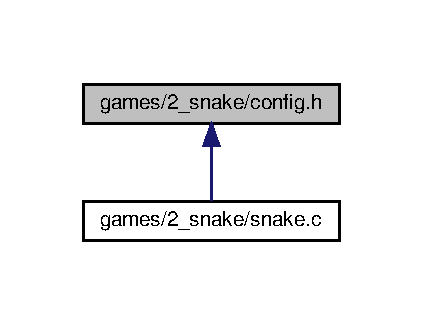
\includegraphics[width=203pt]{2__snake_2config_8h__dep__incl}
\end{center}
\end{figure}
\subsection*{Structures de données}
\begin{DoxyCompactItemize}
\item 
struct \hyperlink{struct_snake_part}{Snake\+Part}
\begin{DoxyCompactList}\small\item\em Contient des informations sur les parties du corps du serpent. \end{DoxyCompactList}\item 
struct \hyperlink{struct_fruit}{Fruit}
\begin{DoxyCompactList}\small\item\em Contient des informations sur les fruits et bonus. \end{DoxyCompactList}\item 
struct \hyperlink{struct_score}{Score}
\begin{DoxyCompactList}\small\item\em Contient des informations sur les affichages de scores individuels. \end{DoxyCompactList}\item 
struct \hyperlink{struct_score_total}{Score\+Total}
\begin{DoxyCompactList}\small\item\em Contient des informations sur le score total. \end{DoxyCompactList}\end{DoxyCompactItemize}
\subsection*{Macros}
\begin{DoxyCompactItemize}
\item 
\#define \hyperlink{2__snake_2config_8h_a598a3330b3c21701223ee0ca14316eca}{PI}~3.\+1415
\item 
\#define \hyperlink{2__snake_2config_8h_ad94200dcde60330427bf06f46d7f8801}{N\+O\+\_\+\+T\+U\+RN}~0
\item 
\#define \hyperlink{2__snake_2config_8h_a437ef08681e7210d6678427030446a54}{L\+E\+FT}~1
\item 
\#define \hyperlink{2__snake_2config_8h_a80fb826a684cf3f0d306b22aa100ddac}{R\+I\+G\+HT}~2
\item 
\#define \hyperlink{2__snake_2config_8h_a53ead818eb14ea44dd094b30347e61f9}{A\+C\+C\+E\+L\+E\+R\+A\+T\+E\+\_\+\+D\+I\+S\+A\+B\+L\+ED}~1
\item 
\#define \hyperlink{2__snake_2config_8h_a63a9c6cffd3b6c045c600545b59602c9}{A\+C\+C\+E\+L\+E\+R\+A\+T\+E\+\_\+\+E\+N\+A\+B\+L\+ED}~2
\item 
\#define \hyperlink{2__snake_2config_8h_afa32d865bca6209bdaf87e7b7ccc9e1a}{H\+IT}~1
\item 
\#define \hyperlink{2__snake_2config_8h_a3c82958aae2c4de245e443b0c89fc15f}{N\+O\+\_\+\+H\+IT}~0
\item 
\#define \hyperlink{2__snake_2config_8h_a017842361bde423abc80e430f9777fe6}{N\+B\+\_\+\+S\+N\+A\+K\+E\+\_\+\+F\+O\+N\+TS}~2
\item 
\#define \hyperlink{2__snake_2config_8h_a8670a6f7b9044ca1ab4cbd8bfcf63050}{N\+B\+\_\+\+S\+N\+A\+K\+E\+\_\+\+S\+O\+U\+N\+DS}~7
\item 
\#define \hyperlink{2__snake_2config_8h_aa6d041de4ad1de2f633476a147823c70}{S\+H\+O\+W\+\_\+\+H\+E\+L\+P\+\_\+\+F\+R\+A\+ME}~20
\item 
\#define \hyperlink{2__snake_2config_8h_a9d79c9ef86bcaecaa1dc2428941d7d19}{R\+E\+L\+A\+Y\+\_\+\+S\+N\+A\+K\+E\+\_\+\+S\+I\+ZE}~15
\item 
\#define \hyperlink{2__snake_2config_8h_a1b16a1176a3dadfdee5fa7a769ba40f8}{S\+I\+Z\+E\+\_\+\+R\+E\+P\+L\+AY}~43.
\item 
\#define \hyperlink{2__snake_2config_8h_aa8d0e37451abf27a2a1fd5a39e197877}{B\+A\+S\+E\+\_\+\+J\+A\+U\+GE}~1.\+6
\item 
\#define \hyperlink{2__snake_2config_8h_a2da0d2e2e194c0cb90f7aba4d60025ed}{F\+R\+A\+M\+E\+\_\+\+J\+A\+U\+G\+E\+\_\+\+A\+N\+IM}~20
\item 
\#define \hyperlink{2__snake_2config_8h_a85f9d29551f1bf30f03229da27cb532f}{F\+R\+A\+M\+E\+S\+\_\+\+P\+E\+R\+\_\+\+S\+E\+C\+O\+ND}~30
\item 
\#define \hyperlink{2__snake_2config_8h_a63a41d21b92cf8804d741dd26d575e26}{B\+O\+D\+Y\+\_\+\+R\+A\+D\+I\+US}~20
\item 
\#define \hyperlink{2__snake_2config_8h_a264f8ff7b542e36fafc9cd08894c80d8}{I\+N\+I\+T\+\_\+\+B\+O\+DY}~30
\item 
\#define \hyperlink{2__snake_2config_8h_a4e8a0f75f21e5116a77c9abead2a886d}{B\+A\+S\+E\+\_\+\+A\+N\+G\+LE}~3 $\ast$ \hyperlink{2__snake_2config_8h_a598a3330b3c21701223ee0ca14316eca}{PI} / 2
\item 
\#define \hyperlink{2__snake_2config_8h_a130e8ced2d3adae7f21e9df296c2a746}{T\+U\+R\+N\+\_\+\+A\+M\+M\+O\+U\+NT}~0.\+13
\item 
\#define \hyperlink{2__snake_2config_8h_affb807bf09880ade28c8c9dc7b67b71b}{R\+E\+M\+I\+N\+D\+\_\+\+B\+O\+DY}~100
\item 
\#define \hyperlink{2__snake_2config_8h_af61077757735b912922d20b17bfe8355}{B\+O\+D\+Y\+\_\+\+D\+E\+A\+T\+H\+\_\+\+H\+I\+T\+B\+OX}~35
\item 
\#define \hyperlink{2__snake_2config_8h_a494b69895fc71ea625fa16ea10b3f5ae}{M\+I\+N\+\_\+\+B\+O\+D\+Y\+\_\+\+P\+A\+R\+TS}~5
\item 
\#define \hyperlink{2__snake_2config_8h_ac947bbf967d5bc8cf3f704388851374d}{N\+B\+\_\+\+F\+R\+A\+M\+E\+\_\+\+D\+E\+A\+T\+H\+\_\+\+B\+O\+DY}~12
\item 
\#define \hyperlink{2__snake_2config_8h_a194de150a51d0e59224c009747f1c2c0}{N\+B\+\_\+\+A\+N\+I\+M\+\_\+\+D\+E\+A\+T\+H\+\_\+\+B\+O\+DY}~4
\item 
\#define \hyperlink{2__snake_2config_8h_adc32f9de2722395f2959d87ba7195728}{N\+B\+\_\+\+F\+R\+A\+M\+E\+\_\+\+I\+N\+V\+I\+N\+C\+I\+B\+I\+L\+I\+TY}~8 $\ast$ \hyperlink{7__asteroid_2config_8h_a85f9d29551f1bf30f03229da27cb532f}{F\+R\+A\+M\+E\+S\+\_\+\+P\+E\+R\+\_\+\+S\+E\+C\+O\+ND}
\item 
\#define \hyperlink{2__snake_2config_8h_ad483314fb15f39afcefd6defa220cc75}{N\+B\+\_\+\+B\+L\+I\+N\+K\+\_\+\+B\+O\+DY}~15
\item 
\#define \hyperlink{2__snake_2config_8h_a417a746fb20389751d14acb47199cc99}{R\+A\+N\+G\+E\+E\+\_\+\+I\+N\+V\+I\+C\+I\+B\+LE}~2
\item 
\#define \hyperlink{2__snake_2config_8h_ac157163ea8e25418e24b630f2732b7b4}{R\+A\+N\+G\+E\+E\+\_\+\+B\+L\+I\+N\+K\+\_\+\+B\+O\+DY}~3
\item 
\#define \hyperlink{2__snake_2config_8h_ad9f1a713cff15b009f0d2918624db3f8}{B\+A\+S\+E\+\_\+\+S\+P\+E\+ED}~7
\item 
\#define \hyperlink{2__snake_2config_8h_ad5f5efaa5cb771bd06da4bfe6046809e}{M\+I\+N\+\_\+\+S\+P\+E\+ED}~5.\+01
\item 
\#define \hyperlink{2__snake_2config_8h_ae8f86c5e3145a02632ce5138a178285e}{S\+P\+E\+E\+D\+\_\+\+D\+E\+C\+O\+M\+P\+O\+S\+I\+T\+I\+ON}~5
\item 
\#define \hyperlink{2__snake_2config_8h_ac0bd8f114faed58760532e4ab0627cee}{S\+C\+A\+L\+E\+\_\+\+S\+P\+E\+ED}~0.\+0035
\item 
\#define \hyperlink{2__snake_2config_8h_a642e16f35aa1e585c25e405ede76e115}{N\+O\+\_\+\+ID}~-\/1
\item 
\#define \hyperlink{2__snake_2config_8h_a3356c494df7432d8a8fc18ba62b06fef}{D\+I\+S\+T\+\_\+\+H\+E\+A\+D\+\_\+\+F\+R\+U\+IT}~30
\item 
\#define \hyperlink{2__snake_2config_8h_a20a685222b1af73857f068beb4da8c29}{D\+I\+S\+T\+\_\+\+W\+A\+L\+L\+\_\+\+F\+R\+U\+IT}~30
\item 
\#define \hyperlink{2__snake_2config_8h_a4136ca081b9c2b0971c330716754aee1}{D\+I\+S\+T\+\_\+\+C\+O\+R\+N\+E\+R\+\_\+\+F\+R\+U\+IT}~60
\item 
\#define \hyperlink{2__snake_2config_8h_a6c8102979ab169311511498b72a4af57}{D\+I\+S\+T\+\_\+\+F\+R\+U\+I\+TS}~10
\item 
\#define \hyperlink{2__snake_2config_8h_ac5d5cf648880cb110dcb850ae806d30c}{R\+A\+N\+G\+E\+E\+\_\+\+B\+L\+I\+NK}~2
\item 
\#define \hyperlink{2__snake_2config_8h_a6545fc609f8f0f93c4243a80a75ef83f}{N\+B\+\_\+\+F\+R\+U\+I\+TS}~25
\item 
\#define \hyperlink{2__snake_2config_8h_a48082f6741c301220f6f5ea34aa238e6}{R\+A\+T\+I\+O\+\_\+\+R\+A\+D\+I\+U\+S\+\_\+\+B\+O\+D\+Y\+A\+DD}~6.\+6
\item 
\#define \hyperlink{2__snake_2config_8h_a952877cd020bb110bc7fc7138347a485}{G\+I\+A\+N\+T\+\_\+\+S\+I\+ZE}~40
\item 
\#define \hyperlink{2__snake_2config_8h_ab9e341e37c83b5dcbc39003064dbf8dd}{G\+I\+A\+N\+T\+\_\+\+D\+I\+G\+E\+S\+T\+I\+ON}~15
\item 
\#define \hyperlink{2__snake_2config_8h_a4f09e32fa4d16806c30286c7246f2251}{G\+I\+A\+N\+T\+\_\+\+S\+C\+O\+RE}~10
\item 
\#define \hyperlink{2__snake_2config_8h_a365f43f09a57ab487955edbe325a286b}{G\+I\+A\+N\+T\+\_\+\+S\+P\+E\+ED}~2
\item 
\#define \hyperlink{2__snake_2config_8h_ae0f1b89533b85cf0ad01d10479fdc389}{U\+N\+L\+O\+C\+K\+\_\+\+G\+I\+A\+NT}~0
\item 
\#define \hyperlink{2__snake_2config_8h_a9d59c70aaa40ea44cea401e31416adeb}{G\+I\+A\+N\+T\+\_\+\+C\+H\+A\+N\+CE}~200
\item 
\#define \hyperlink{2__snake_2config_8h_a1cc90d02dc3aaf3b97a83bc07be75d99}{M\+A\+X\+\_\+\+T\+R\+I\+E\+S\+\_\+\+R\+A\+ND}~100
\item 
\#define \hyperlink{2__snake_2config_8h_a659431efcb0fb778fbc65669d799467f}{C\+H\+A\+N\+C\+E\+\_\+\+S\+P\+A\+W\+N\+\_\+\+F\+R\+U\+IT}~((int)(1 $\ast$ \hyperlink{7__asteroid_2config_8h_a85f9d29551f1bf30f03229da27cb532f}{F\+R\+A\+M\+E\+S\+\_\+\+P\+E\+R\+\_\+\+S\+E\+C\+O\+ND}))
\item 
\#define \hyperlink{2__snake_2config_8h_a6d6d565ebf5514e02485cbc6e0056b0c}{C\+H\+A\+N\+C\+E\+\_\+\+S\+P\+A\+W\+N\+\_\+\+F\+R\+U\+I\+T\+\_\+\+H\+A\+R\+D\+C\+O\+R\+E\+\_\+\+I\+N\+IT}~6
\item 
\#define \hyperlink{2__snake_2config_8h_a2537f410dcf058d30b4132bc7fbf33f6}{C\+H\+A\+N\+C\+E\+\_\+\+S\+P\+A\+W\+N\+\_\+\+F\+R\+U\+I\+T\+\_\+\+H\+A\+R\+D\+C\+O\+R\+E\+\_\+\+M\+IN}~1.\+6
\item 
\#define \hyperlink{2__snake_2config_8h_ab4a64af6bbd2f79828925c21caba74f4}{C\+H\+A\+N\+C\+E\+\_\+\+S\+P\+A\+W\+N\+\_\+\+F\+R\+U\+I\+T\+\_\+\+H\+A\+R\+D\+C\+O\+R\+E\+\_\+\+R\+A\+TE}~((\hyperlink{2__snake_2config_8h_a6d6d565ebf5514e02485cbc6e0056b0c}{C\+H\+A\+N\+C\+E\+\_\+\+S\+P\+A\+W\+N\+\_\+\+F\+R\+U\+I\+T\+\_\+\+H\+A\+R\+D\+C\+O\+R\+E\+\_\+\+I\+N\+IT} -\/ \hyperlink{2__snake_2config_8h_a2537f410dcf058d30b4132bc7fbf33f6}{C\+H\+A\+N\+C\+E\+\_\+\+S\+P\+A\+W\+N\+\_\+\+F\+R\+U\+I\+T\+\_\+\+H\+A\+R\+D\+C\+O\+R\+E\+\_\+\+M\+IN}) / (3.$\ast$60 $\ast$ \hyperlink{7__asteroid_2config_8h_a85f9d29551f1bf30f03229da27cb532f}{F\+R\+A\+M\+E\+S\+\_\+\+P\+E\+R\+\_\+\+S\+E\+C\+O\+ND}))
\item 
\#define \hyperlink{2__snake_2config_8h_a8e15577df297c755902c6f004418dea0}{F\+R\+U\+I\+T\+\_\+\+T\+TL}~(\hyperlink{7__asteroid_2config_8h_a85f9d29551f1bf30f03229da27cb532f}{F\+R\+A\+M\+E\+S\+\_\+\+P\+E\+R\+\_\+\+S\+E\+C\+O\+ND} $\ast$ 14)
\item 
\#define \hyperlink{2__snake_2config_8h_a40dae4de9a3168931b46241e438e091a}{N\+B\+\_\+\+F\+R\+A\+M\+E\+\_\+\+S\+P\+A\+W\+N\+\_\+\+F\+R\+U\+IT}~12
\item 
\#define \hyperlink{2__snake_2config_8h_a7bfe0432c75a359bcd3f643f67869442}{N\+B\+\_\+\+A\+N\+I\+M\+\_\+\+S\+P\+A\+WN}~4
\item 
\#define \hyperlink{2__snake_2config_8h_ae122be164dcf6bcaef5d3fe7fb26e2b2}{N\+B\+\_\+\+F\+R\+A\+M\+E\+\_\+\+D\+E\+A\+T\+H\+\_\+\+F\+R\+U\+IT}~12
\item 
\#define \hyperlink{2__snake_2config_8h_aaffd5302153b1f4887574eed8b0101ca}{N\+B\+\_\+\+A\+N\+I\+M\+\_\+\+D\+E\+A\+TH}~4
\item 
\#define \hyperlink{2__snake_2config_8h_a583645970a23f5d70084e040123ddb61}{F\+R\+O\+M\+\_\+\+N\+A\+T\+U\+R\+AL}~0
\item 
\#define \hyperlink{2__snake_2config_8h_a8cde5dd34318fd1145d2caeab997270c}{F\+R\+O\+M\+\_\+\+C\+O\+F\+F\+RE}~1
\item 
\#define \hyperlink{2__snake_2config_8h_a61e1db40665c11aadcdff338fac8dda2}{F\+R\+O\+M\+\_\+\+R\+A\+I\+N\+B\+OW}~2
\item 
\#define \hyperlink{2__snake_2config_8h_a49e2dea00028a9e4388ba0e307d8bef7}{H\+I\+T\+B\+O\+X\+\_\+\+S\+E\+C\+U\+R\+I\+TY}~1
\item 
\#define \hyperlink{2__snake_2config_8h_a96100f98706782fd5de0b48bb85aaa32}{H\+I\+T\+B\+O\+X\+\_\+\+G\+E\+N\+T\+I\+L\+LE}~2.\+33
\item 
\#define \hyperlink{2__snake_2config_8h_a423401e070b1371ab937c7deee94f02f}{R\+A\+T\+I\+O\+\_\+\+R\+A\+D\+I\+U\+S\+\_\+\+H\+A\+R\+D\+C\+O\+RE}~0.\+8
\item 
\#define \hyperlink{2__snake_2config_8h_a4b43ca180ce48e803e6cf1a7e40e9f53}{R\+A\+T\+I\+O\+\_\+\+S\+P\+E\+E\+D\+\_\+\+H\+A\+R\+D\+C\+O\+RE}~5
\item 
\#define \hyperlink{2__snake_2config_8h_a3de8ac1f84acb49aa878ddc7c85945af}{R\+A\+T\+I\+O\+\_\+\+G\+E\+T\+\_\+\+F\+R\+U\+I\+T\+\_\+\+H\+A\+R\+D\+C\+O\+RE}~-\/5
\item 
\#define \hyperlink{2__snake_2config_8h_aee59e903d5ea66e6c82b668d52fd6230}{F\+R\+U\+I\+T\+\_\+\+E\+A\+T\+E\+N\+\_\+\+H\+A\+R\+D\+C\+O\+RE}~-\/5
\item 
\#define \hyperlink{2__snake_2config_8h_af59c26c956936f6269c011c945d9e1a1}{F\+R\+U\+I\+T\+\_\+\+T\+I\+M\+E\+O\+U\+T\+\_\+\+E\+A\+T\+E\+N\+\_\+\+H\+A\+R\+D\+C\+O\+RE}~0.\+18
\item 
\#define \hyperlink{2__snake_2config_8h_ad755ce3d83234d9bd4130ad1563460e7}{F\+R\+U\+I\+T\+\_\+\+T\+I\+M\+E\+O\+U\+T\+\_\+\+S\+C\+O\+R\+E\+\_\+\+H\+A\+R\+D\+C\+O\+RE}~0.\+25
\item 
\#define \hyperlink{2__snake_2config_8h_a93902b8fbe14a1e41933fb52b60edaa8}{R\+A\+T\+I\+O\+\_\+\+T\+T\+L\+\_\+\+H\+A\+R\+D\+C\+O\+RE}~0.\+5
\item 
\#define \hyperlink{2__snake_2config_8h_adf1eb896471dfb54a59e84fb5d7a1d7a}{P\+R\+E\+C\+I\+S\+I\+O\+N\+\_\+\+S\+P\+A\+WN}~100
\item 
\#define \hyperlink{2__snake_2config_8h_a4086933ab42df07b6c002e050061c66a}{F\+L\+A\+T\+\_\+\+R\+E\+D\+U\+C\+E\+\_\+\+S\+C\+I\+S\+OR}~10
\item 
\#define \hyperlink{2__snake_2config_8h_af5d8410e06a63c683971d97da7179cb8}{R\+E\+L\+A\+T\+I\+V\+E\+\_\+\+R\+E\+D\+U\+C\+E\+\_\+\+S\+C\+I\+S\+OR}~0.\+15
\item 
\#define \hyperlink{2__snake_2config_8h_a38a47f3cb92d1ecd87fd388fd89a647e}{D\+U\+R\+A\+T\+I\+O\+N\+\_\+\+P\+O\+T\+I\+ON}~180
\item 
\#define \hyperlink{2__snake_2config_8h_a9848c1ecd894623b78c8cc04241cddfe}{R\+E\+L\+A\+T\+I\+V\+E\+\_\+\+A\+C\+C\+E\+L\+E\+R\+A\+T\+E\+\_\+\+C\+O\+F\+EE}~0.\+25
\item 
\#define \hyperlink{2__snake_2config_8h_aa5c414cc45eec8bd806bec316d058444}{N\+B\+\_\+\+B\+O\+N\+U\+S\+ES}~7
\item 
\#define \hyperlink{2__snake_2config_8h_a8ef4427b56d7615696b43061dac8b8a6}{C\+H\+A\+N\+C\+E\+\_\+\+S\+P\+A\+W\+N\+\_\+\+B\+O\+N\+US}~(12 $\ast$ \hyperlink{7__asteroid_2config_8h_a85f9d29551f1bf30f03229da27cb532f}{F\+R\+A\+M\+E\+S\+\_\+\+P\+E\+R\+\_\+\+S\+E\+C\+O\+ND})
\item 
\#define \hyperlink{2__snake_2config_8h_a7a879adc899a78b15721b21491d8f245}{F\+L\+A\+T\+\_\+\+R\+M\+\_\+\+B\+O\+MB}~10
\item 
\#define \hyperlink{2__snake_2config_8h_aa6d9af45fa40a70e976cf33f13413ea3}{R\+E\+L\+A\+T\+I\+V\+E\+\_\+\+R\+M\+\_\+\+B\+O\+MB}~0.\+2
\item 
\#define \hyperlink{2__snake_2config_8h_a9dae1bd3dded89d3c160ad30004c7a1d}{R\+E\+L\+A\+T\+I\+V\+E\+\_\+\+S\+L\+O\+W\+\_\+\+F\+E\+A\+T\+H\+ER}~0.\+3
\item 
\#define \hyperlink{2__snake_2config_8h_ab1f6b58f70ac42ec3e39304f8f716d6d}{C\+O\+F\+F\+R\+E\+\_\+\+S\+P\+A\+W\+N\+\_\+\+M\+IN}~50
\item 
\#define \hyperlink{2__snake_2config_8h_ac92ade727da8bc7ebb39945c137a1c47}{C\+O\+F\+F\+R\+E\+\_\+\+S\+P\+A\+W\+N\+\_\+\+R\+A\+N\+GE}~100
\item 
\#define \hyperlink{2__snake_2config_8h_a2a4d2752f4ca8389fe5a269e6cbadb70}{N\+B\+\_\+\+S\+P\+A\+W\+N\+\_\+\+C\+O\+F\+F\+RE}~6
\item 
\#define \hyperlink{2__snake_2config_8h_a7e375690ed8c4fd75c3c9db3843cbe88}{C\+H\+E\+S\+T\+\_\+\+B\+O\+O\+S\+T\+\_\+\+F\+R\+U\+I\+T\+\_\+\+E\+A\+T\+EN}~5
\item 
\#define \hyperlink{2__snake_2config_8h_ae6a8d05b42d1fdeab862b44aad7ebe4a}{F\+R\+A\+M\+E\+\_\+\+R\+E\+T\+A\+R\+D\+\_\+\+C\+O\+F\+F\+RE}~2
\item 
\#define \hyperlink{2__snake_2config_8h_a3dfb7bad8ad543d6b7c5fb30b767124e}{N\+B\+\_\+\+S\+P\+A\+W\+N\+\_\+\+A\+R\+C\+\_\+\+E\+N\+\_\+\+C\+I\+EL}~12
\item 
\#define \hyperlink{2__snake_2config_8h_af5a17b33bfb1537ee8dc7ebe7e3170d5}{R\+A\+I\+N\+B\+O\+W\+\_\+\+B\+O\+O\+S\+T\+\_\+\+F\+R\+U\+I\+T\+\_\+\+E\+A\+T\+EN}~5
\item 
\#define \hyperlink{2__snake_2config_8h_a99314816a5eaf447e8eedc381b97bbce}{D\+I\+S\+T\+\_\+\+W\+A\+L\+L\+\_\+\+F\+R\+U\+I\+T\+\_\+\+R\+A\+I\+N\+B\+OW}~80
\item 
\#define \hyperlink{2__snake_2config_8h_aa50a54b6ec00686451c64225e946cd93}{F\+R\+A\+M\+E\+\_\+\+R\+E\+T\+A\+R\+D\+\_\+\+R\+A\+I\+N\+B\+OW}~3
\item 
\#define \hyperlink{2__snake_2config_8h_acf8d0734fe4a07ca696a59c55fc8cf3e}{P\+O\+T\+I\+O\+N\+\_\+\+P\+O\+I\+S\+O\+N\+\_\+\+A\+DD}~(1.\+5 / \hyperlink{7__asteroid_2config_8h_a85f9d29551f1bf30f03229da27cb532f}{F\+R\+A\+M\+E\+S\+\_\+\+P\+E\+R\+\_\+\+S\+E\+C\+O\+ND})
\item 
\#define \hyperlink{2__snake_2config_8h_a2c5c4f395834ec9d9bb2263c3a90d3c5}{P\+O\+I\+S\+O\+N\+\_\+\+S\+C\+A\+LE}~1.\+001
\item 
\#define \hyperlink{2__snake_2config_8h_af4f0586763b18c7fbb87d7964f724dec}{B\+O\+M\+B\+\_\+\+T\+E\+X\+T\+U\+R\+E\+\_\+\+R\+A\+TE}~4
\item 
\#define \hyperlink{2__snake_2config_8h_abf76ac1009f977447152232bab4bbeee}{E\+S\+P\+A\+C\+E\+M\+E\+N\+T\+\_\+\+S\+H\+O\+W\+\_\+\+P\+O\+T\+I\+ON}~70
\item 
\#define \hyperlink{2__snake_2config_8h_a99919f51a0981bd5cf0cb811abc30aa8}{N\+B\+\_\+\+P\+O\+T\+I\+O\+N\+\_\+\+M\+AX}~5
\item 
\#define \hyperlink{2__snake_2config_8h_a452d9b7fb36cd72dc9e515db32016c81}{M\+A\+X\+\_\+\+B\+O\+M\+B\+\_\+\+S\+I\+ZE}~700
\item 
\#define \hyperlink{2__snake_2config_8h_ad907fc45a21d1c430b343bc8c727fa5b}{N\+B\+\_\+\+F\+R\+A\+M\+E\+\_\+\+C\+A\+F\+E\+\_\+\+A\+C\+CE}~(4 $\ast$ \hyperlink{7__asteroid_2config_8h_a85f9d29551f1bf30f03229da27cb532f}{F\+R\+A\+M\+E\+S\+\_\+\+P\+E\+R\+\_\+\+S\+E\+C\+O\+ND})
\item 
\#define \hyperlink{2__snake_2config_8h_aa07bb12ffaa00b6029beb6c440d6f9f6}{F\+I\+N\+A\+L\+\_\+\+D\+E\+A\+T\+H\+\_\+\+R\+A\+T\+E\+\_\+\+I\+N\+IT}~(9. / \hyperlink{7__asteroid_2config_8h_a85f9d29551f1bf30f03229da27cb532f}{F\+R\+A\+M\+E\+S\+\_\+\+P\+E\+R\+\_\+\+S\+E\+C\+O\+ND})
\item 
\#define \hyperlink{2__snake_2config_8h_ad148d10d93ddee35ed48e5b7bffb571d}{F\+I\+N\+A\+L\+\_\+\+D\+E\+A\+T\+H\+\_\+\+R\+A\+T\+E\+\_\+\+G\+R\+OW}~1.\+03
\item 
\#define \hyperlink{2__snake_2config_8h_ae09e7f8485a8daa0867e04e3d352223e}{F\+I\+N\+A\+L\+\_\+\+D\+E\+A\+T\+H\+\_\+\+M\+AX}~(12. / \hyperlink{7__asteroid_2config_8h_a85f9d29551f1bf30f03229da27cb532f}{F\+R\+A\+M\+E\+S\+\_\+\+P\+E\+R\+\_\+\+S\+E\+C\+O\+ND})
\item 
\#define \hyperlink{2__snake_2config_8h_a53066bae2a065f358a9534d3b69248cf}{I\+N\+I\+T\+\_\+\+F\+R\+A\+M\+E\+\_\+\+D\+E\+A\+TH}~4
\item 
\#define \hyperlink{2__snake_2config_8h_a49d3e07d0476c6025604c90432729f7e}{N\+B\+\_\+\+C\+H\+A\+R\+\_\+\+A\+F\+F\+I\+C\+H\+A\+G\+E\+\_\+\+S\+C\+O\+RE}~21
\item 
\#define \hyperlink{2__snake_2config_8h_a0ebf185842674cdecc6621333d79f8a5}{F\+R\+A\+M\+E\+\_\+\+S\+C\+O\+R\+E\+\_\+\+A\+N\+IM}~20
\item 
\#define \hyperlink{2__snake_2config_8h_a0e5a3398e5c056c631be474eddfd88f7}{M\+I\+N\+\_\+\+S\+I\+Z\+E\+\_\+\+S\+C\+O\+RE}~22
\item 
\#define \hyperlink{2__snake_2config_8h_a0c59830d341e0be804b4d038403e5d21}{M\+A\+X\+\_\+\+S\+I\+Z\+E\+\_\+\+S\+C\+O\+RE}~45
\item 
\#define \hyperlink{2__snake_2config_8h_a6c9f2388e91c636203c0ac7d7e675899}{S\+C\+O\+R\+E\+\_\+\+T\+TL}~20
\item 
\#define \hyperlink{2__snake_2config_8h_afdde5ee34f7e3a12bf31303ddd82d0f8}{F\+O\+N\+T\+\_\+\+H\+E\+I\+G\+H\+T\+\_\+\+R\+A\+T\+IO}~1.\+5
\item 
\#define \hyperlink{2__snake_2config_8h_a40b37952c6304be53405426099855e90}{N\+B\+\_\+\+B\+L\+I\+NK}~15
\item 
\#define \hyperlink{2__snake_2config_8h_a4f758bb3e6e5ec43907290e0ded9c92e}{N\+B\+\_\+\+P\+R\+O\+P\+R\+I\+E\+T\+ES}~6
\item 
\#define \hyperlink{2__snake_2config_8h_ad98436000e18335092caefd6cd7acbc1}{A\+P\+P\+E\+A\+R\+\_\+\+M\+AX}~50.
\item 
\#define \hyperlink{2__snake_2config_8h_ace456e507e9273d5ac294db0eadeca08}{S\+I\+Z\+E\+\_\+\+P\+R\+E\+\_\+\+R\+A\+D\+I\+US}~31
\end{DoxyCompactItemize}
\subsection*{Énumérations}
\begin{DoxyCompactItemize}
\item 
enum \hyperlink{2__snake_2config_8h_a95d3172c264d2e03684617fc88363e89}{T\+\_\+\+F\+O\+N\+TS} \{ \hyperlink{2__snake_2config_8h_a95d3172c264d2e03684617fc88363e89af5264f27fa478da40ccabc5924f59945}{S\+\_\+\+B\+A\+S\+E\+\_\+\+F\+O\+NT}, 
\hyperlink{2__snake_2config_8h_a95d3172c264d2e03684617fc88363e89a91d5d5ef298cc29d3c15bc1aac42fa36}{S\+\_\+\+F\+L\+A\+P\+PY}, 
\hyperlink{5__tetris_2config_8h_a95d3172c264d2e03684617fc88363e89aee115797fde6f9637eb4d69dcc52dac6}{T\+\_\+\+F\+O\+N\+T\+\_\+\+C\+O\+M\+BO}
 \}
\item 
enum \{ \newline
\hyperlink{2__snake_2config_8h_abc6126af1d45847bc59afa0aa3216b04a9d57b1d925fa2a89ff271a2395fa4ce0}{S\+O\+U\+N\+D\+\_\+\+R\+A\+I\+N\+B\+OW}, 
\hyperlink{2__snake_2config_8h_abc6126af1d45847bc59afa0aa3216b04ac1822f280f0bf4d2ae1f1730e4411398}{S\+O\+U\+N\+D\+\_\+\+B\+O\+MB}, 
\hyperlink{2__snake_2config_8h_abc6126af1d45847bc59afa0aa3216b04ae4f19f5c3069c77e8320706310e1e88e}{S\+O\+U\+N\+D\+\_\+\+S\+L\+OW}, 
\hyperlink{2__snake_2config_8h_abc6126af1d45847bc59afa0aa3216b04a3590463c30b0dc5c9a76c76e06fb609d}{S\+O\+U\+N\+D\+\_\+\+G\+ET}, 
\newline
\hyperlink{2__snake_2config_8h_abc6126af1d45847bc59afa0aa3216b04a9874ae2472ac440a37243b9fc2173201}{S\+O\+U\+N\+D\+\_\+\+A\+P\+P\+E\+AR}, 
\hyperlink{2__snake_2config_8h_abc6126af1d45847bc59afa0aa3216b04a9cd3c44a68fd843867f117759fd3fb94}{S\+O\+U\+N\+D\+\_\+\+D\+I\+S\+A\+P\+E\+AR}, 
\hyperlink{2__snake_2config_8h_abc6126af1d45847bc59afa0aa3216b04a3c84a26eed13f1442e465fd3b2e64434}{S\+O\+U\+N\+D\+\_\+\+G\+A\+M\+E\+O\+V\+ER}
 \}
\item 
enum \hyperlink{2__snake_2config_8h_a9aaea59f6de3d04ec41058e7aa50f938}{F\+R\+U\+I\+TS} \{ \newline
\hyperlink{2__snake_2config_8h_a9aaea59f6de3d04ec41058e7aa50f938a3892c3dac5b5a2a4ca54ffef8e048215}{F\+R\+A\+I\+SE}, 
\hyperlink{2__snake_2config_8h_a9aaea59f6de3d04ec41058e7aa50f938ace9ee4c1a6b777940c7f3a766a9a88d4}{O\+R\+A\+N\+GE}, 
\hyperlink{2__snake_2config_8h_a9aaea59f6de3d04ec41058e7aa50f938a3432ae8663a96c7bf0a13ca206c69ea8}{C\+I\+T\+R\+O\+U\+I\+L\+LE}, 
\hyperlink{2__snake_2config_8h_a9aaea59f6de3d04ec41058e7aa50f938a426ea7de1c60f9aad0a537f16540440e}{P\+I\+M\+E\+NT}, 
\newline
\hyperlink{2__snake_2config_8h_a9aaea59f6de3d04ec41058e7aa50f938aa27e898f03ce86e645cd973fc0a79cd3}{C\+E\+R\+I\+SE}, 
\hyperlink{2__snake_2config_8h_a9aaea59f6de3d04ec41058e7aa50f938a84b9fa7009b1cc02cd496953dab8229d}{P\+O\+M\+ME}, 
\hyperlink{2__snake_2config_8h_a9aaea59f6de3d04ec41058e7aa50f938a4f8c3e9749330ba8c5ced345da8e8517}{P\+A\+S\+T\+E\+Q\+UE}, 
\hyperlink{2__snake_2config_8h_a9aaea59f6de3d04ec41058e7aa50f938a81b731da1e1e223f375bc92ed7ce8227}{C\+A\+R\+O\+T\+TE}, 
\newline
\hyperlink{2__snake_2config_8h_a9aaea59f6de3d04ec41058e7aa50f938a16cab635594f069387a7fca5e06e20de}{A\+N\+A\+N\+AS}, 
\hyperlink{2__snake_2config_8h_a9aaea59f6de3d04ec41058e7aa50f938a21630e9c9bbde9814f436fdbf5f4aee8}{T\+O\+M\+A\+TE}, 
\hyperlink{2__snake_2config_8h_a9aaea59f6de3d04ec41058e7aa50f938a40b116a22554b16c1544597cccb78c30}{F\+R\+O\+M\+A\+GE}, 
\hyperlink{2__snake_2config_8h_a9aaea59f6de3d04ec41058e7aa50f938a53c6aa2804050e4d2ba15aaf8e80cfd1}{V\+I\+A\+N\+DE}, 
\newline
\hyperlink{2__snake_2config_8h_a9aaea59f6de3d04ec41058e7aa50f938a4d4253ddfb8b2ca0ed658953283c79fa}{P\+I\+Z\+ZA}, 
\hyperlink{2__snake_2config_8h_a9aaea59f6de3d04ec41058e7aa50f938ad18309fbba10f792a5218257dbfa46f4}{B\+U\+R\+G\+ER}, 
\hyperlink{2__snake_2config_8h_a9aaea59f6de3d04ec41058e7aa50f938a23ed9ec8bef16eed197ffc6d56603eb4}{H\+O\+T\+\_\+\+D\+OG}, 
\hyperlink{2__snake_2config_8h_a9aaea59f6de3d04ec41058e7aa50f938ab7dc7deb6aa12f9e166a6a9ff36f7a73}{P\+A\+N\+C\+A\+K\+ES}, 
\newline
\hyperlink{2__snake_2config_8h_a9aaea59f6de3d04ec41058e7aa50f938aa4cf9e98c8645011e11b84edc21c8329}{S\+U\+C\+E\+T\+TE}, 
\hyperlink{2__snake_2config_8h_a9aaea59f6de3d04ec41058e7aa50f938a032d1c005889dab1db685c62def2da4a}{G\+L\+A\+C\+E\+\_\+\+B\+A\+T\+ON}, 
\hyperlink{2__snake_2config_8h_a9aaea59f6de3d04ec41058e7aa50f938a5e8ab0e57a55ba1db0f3c65605b1389c}{G\+L\+A\+C\+E\+\_\+\+C\+O\+NE}, 
\hyperlink{2__snake_2config_8h_a9aaea59f6de3d04ec41058e7aa50f938af7c838e07617f7c5bd0c36296be8e330}{G\+L\+A\+C\+E\+\_\+\+P\+OT}, 
\newline
\hyperlink{2__snake_2config_8h_a9aaea59f6de3d04ec41058e7aa50f938a232c1030acbe27eaf013c94167fffa1e}{D\+O\+N\+UT}, 
\hyperlink{2__snake_2config_8h_a9aaea59f6de3d04ec41058e7aa50f938a939a3431dedcdf375ad000308aa68289}{M\+U\+F\+F\+IN}, 
\hyperlink{2__snake_2config_8h_a9aaea59f6de3d04ec41058e7aa50f938a00c134642b071771eb85d744a31fe618}{G\+A\+T\+E\+AU}, 
\hyperlink{2__snake_2config_8h_a9aaea59f6de3d04ec41058e7aa50f938a5d3be7fd84a125a35f8e6b180af8894b}{M\+U\+F\+F\+I\+N\+\_\+\+R\+O\+SE}, 
\newline
\hyperlink{2__snake_2config_8h_a9aaea59f6de3d04ec41058e7aa50f938a87df4632985ef4962326b2363ea36e9c}{C\+A\+FE}, 
\hyperlink{2__snake_2config_8h_a9aaea59f6de3d04ec41058e7aa50f938a080e2bcc27043ac0b228d092e18430f6}{P\+L\+U\+ME}, 
\hyperlink{2__snake_2config_8h_a9aaea59f6de3d04ec41058e7aa50f938a43890ace4b17eeb14f1ba9fcc4466433}{B\+O\+M\+BE}, 
\hyperlink{2__snake_2config_8h_a9aaea59f6de3d04ec41058e7aa50f938a9b1762c454fdf89bcabc30b8452c1b5c}{C\+O\+F\+F\+RE}, 
\newline
\hyperlink{2__snake_2config_8h_a9aaea59f6de3d04ec41058e7aa50f938a3edc0c4dab4f09703dac9ac2f1026c03}{A\+R\+C\+\_\+\+E\+N\+\_\+\+C\+I\+EL}, 
\hyperlink{2__snake_2config_8h_a9aaea59f6de3d04ec41058e7aa50f938a2c8270a74fbdf1d391d10ce5619ebaa6}{P\+O\+T\+I\+O\+N\+\_\+\+H\+I\+T\+B\+OX}, 
\hyperlink{2__snake_2config_8h_a9aaea59f6de3d04ec41058e7aa50f938a89f6340654240c96252d7d3c6bf51fac}{P\+O\+T\+I\+O\+N\+\_\+\+V\+E\+R\+TE}, 
\hyperlink{2__snake_2config_8h_a9aaea59f6de3d04ec41058e7aa50f938ab085d8b8379ba0d3bdea7ed9f8089394}{P\+O\+T\+I\+O\+N\+\_\+\+J\+A\+U\+NE}
 \}
\item 
enum \hyperlink{2__snake_2config_8h_adad37480173ed85053413758cf15fe30}{P\+R\+O\+P\+R\+I\+E\+T\+ES} \{ \newline
\hyperlink{2__snake_2config_8h_adad37480173ed85053413758cf15fe30acc313c985549b695d777b0cd3d772555}{A\+C\+C\+E\+L\+E\+R\+A\+T\+I\+ON}, 
\hyperlink{2__snake_2config_8h_adad37480173ed85053413758cf15fe30ab599bb1cb8b8b74571549d37220d5e5f}{R\+A\+D\+I\+US}, 
\hyperlink{2__snake_2config_8h_adad37480173ed85053413758cf15fe30ae8e6f1dc1a169dad23a94b63ed1d4cb3}{P\+R\+O\+BA}, 
\hyperlink{2__snake_2config_8h_adad37480173ed85053413758cf15fe30af57444a2814db96222f09035ff269767}{S\+C\+O\+RE}, 
\newline
\hyperlink{2__snake_2config_8h_adad37480173ed85053413758cf15fe30ae7dfc3e4aa958f8b389e3614acf60500}{D\+I\+G\+E\+S\+T\+I\+O\+N\+\_\+\+S\+I\+ZE}, 
\hyperlink{2__snake_2config_8h_adad37480173ed85053413758cf15fe30aa461a57101a6a16d39204225434d02ac}{M\+I\+N\+\_\+\+F\+R\+U\+I\+T\+\_\+\+T\+O\+\_\+\+A\+P\+P\+E\+AR}
 \}
\end{DoxyCompactItemize}
\subsection*{Variables}
\begin{DoxyCompactItemize}
\item 
const S\+D\+L\+\_\+\+Point \hyperlink{2__snake_2config_8h_a968d31411239df4ea501d92b69ce6548}{E\+S\+P\+A\+C\+E\+\_\+\+D\+I\+S\+P\+L\+A\+Y\+\_\+\+W\+I\+N\+D\+OW} = \{67, 57\}
\item 
const Vector2f \hyperlink{2__snake_2config_8h_a7267ba84becc750838c6191fed2ba14c}{U\+N\+D\+EF} = \{-\/500, -\/500\}
\item 
char $\ast$ \hyperlink{2__snake_2config_8h_adbfb2293a32d42faa82f7c43beca7869}{D\+I\+R\+\_\+\+F\+O\+N\+T\+S\+\_\+\+S\+N\+A\+KE} \mbox{[}\hyperlink{2__snake_2config_8h_a017842361bde423abc80e430f9777fe6}{N\+B\+\_\+\+S\+N\+A\+K\+E\+\_\+\+F\+O\+N\+TS}\mbox{]}
\item 
char $\ast$ \hyperlink{2__snake_2config_8h_abf04e5e75be076a34f769380ef4e4e9d}{D\+I\+R\+\_\+\+S\+O\+U\+N\+D\+S\+\_\+\+S\+N\+A\+KE} \mbox{[}\hyperlink{2__snake_2config_8h_a8670a6f7b9044ca1ab4cbd8bfcf63050}{N\+B\+\_\+\+S\+N\+A\+K\+E\+\_\+\+S\+O\+U\+N\+DS}\mbox{]}
\item 
static int \hyperlink{2__snake_2config_8h_a9c9d7769debc1a650964c979920c5da2}{S\+O\+U\+N\+D\+\_\+\+V\+O\+L\+U\+M\+ES} \mbox{[}\hyperlink{2__snake_2config_8h_a8670a6f7b9044ca1ab4cbd8bfcf63050}{N\+B\+\_\+\+S\+N\+A\+K\+E\+\_\+\+S\+O\+U\+N\+DS}\mbox{]} = \{70,128,80,55,13, 18,100\}
\item 
S\+D\+L\+\_\+\+Rect \hyperlink{2__snake_2config_8h_a9b1d125f3b82f826622c2155834be514}{B\+A\+S\+K\+E\+T\+\_\+\+D\+IM} = \{0, 0, 62, 950\}
\item 
S\+D\+L\+\_\+\+Color \hyperlink{2__snake_2config_8h_acc130135e04e013d81f4763e1f439444}{C\+O\+L\+O\+R\+\_\+\+J\+A\+U\+G\+E\+\_\+\+B\+A\+CK} = \{0x56,0x46,0x3b\}
\item 
S\+D\+L\+\_\+\+Color \hyperlink{2__snake_2config_8h_a40076320a4ff1a9565bf3f806584a955}{C\+O\+L\+O\+R\+\_\+\+J\+A\+U\+GE} = \{0x77,0xcd,0x44\}
\item 
static const int \hyperlink{2__snake_2config_8h_a1563e736047cb57052434e132e4afac4}{F\+R\+A\+M\+E\+\_\+\+T\+I\+ME} = 1000 / \hyperlink{7__asteroid_2config_8h_a85f9d29551f1bf30f03229da27cb532f}{F\+R\+A\+M\+E\+S\+\_\+\+P\+E\+R\+\_\+\+S\+E\+C\+O\+ND}
\item 
S\+D\+L\+\_\+\+Color \hyperlink{2__snake_2config_8h_a44ea80ea1f758a8127cf1ecc32b297fb}{H\+U\+D\+\_\+\+C\+O\+L\+OR} = \{138,82,47\}
\item 
const Vector2f \hyperlink{2__snake_2config_8h_a3a86095c40877647a4d84ab17880049c}{I\+N\+I\+T\+\_\+\+H\+E\+AD} = \{P\+L\+A\+Y\+G\+R\+O\+U\+N\+D\+\_\+\+S\+I\+Z\+E\+\_\+W / 2, P\+L\+A\+Y\+G\+R\+O\+U\+N\+D\+\_\+\+S\+I\+Z\+E\+\_\+H / 2\}
\item 
const Vector2f \hyperlink{2__snake_2config_8h_a9db0cb4175480807da74717f9a68d61f}{I\+N\+I\+T\+\_\+\+D\+E\+C\+AL} = \{0, 5\}
\item 
const S\+D\+L\+\_\+\+Point \hyperlink{2__snake_2config_8h_afc11d833a89fae1a7fa492711e229d7d}{B\+O\+D\+Y\+\_\+\+D\+IM} = \{64, 64\}
\item 
const int \hyperlink{2__snake_2config_8h_adc0ba100340886b25845ff4f4015f23a}{B\+L\+I\+N\+K\+\_\+\+F\+R\+A\+M\+E\+S\+\_\+\+B\+O\+DY} \mbox{[}\hyperlink{2__snake_2config_8h_ad483314fb15f39afcefd6defa220cc75}{N\+B\+\_\+\+B\+L\+I\+N\+K\+\_\+\+B\+O\+DY}\mbox{]} = \{(int)(\hyperlink{7__asteroid_2config_8h_a85f9d29551f1bf30f03229da27cb532f}{F\+R\+A\+M\+E\+S\+\_\+\+P\+E\+R\+\_\+\+S\+E\+C\+O\+ND} $\ast$ 4.\+5 + ((\hyperlink{2__snake_2config_8h_adc32f9de2722395f2959d87ba7195728}{N\+B\+\_\+\+F\+R\+A\+M\+E\+\_\+\+I\+N\+V\+I\+N\+C\+I\+B\+I\+L\+I\+TY} / \hyperlink{7__asteroid_2config_8h_a85f9d29551f1bf30f03229da27cb532f}{F\+R\+A\+M\+E\+S\+\_\+\+P\+E\+R\+\_\+\+S\+E\+C\+O\+ND}) -\/ 8) $\ast$ \hyperlink{7__asteroid_2config_8h_a85f9d29551f1bf30f03229da27cb532f}{F\+R\+A\+M\+E\+S\+\_\+\+P\+E\+R\+\_\+\+S\+E\+C\+O\+ND}), (int)(\hyperlink{7__asteroid_2config_8h_a85f9d29551f1bf30f03229da27cb532f}{F\+R\+A\+M\+E\+S\+\_\+\+P\+E\+R\+\_\+\+S\+E\+C\+O\+ND} $\ast$ 5.\+3 + ((\hyperlink{2__snake_2config_8h_adc32f9de2722395f2959d87ba7195728}{N\+B\+\_\+\+F\+R\+A\+M\+E\+\_\+\+I\+N\+V\+I\+N\+C\+I\+B\+I\+L\+I\+TY} / \hyperlink{7__asteroid_2config_8h_a85f9d29551f1bf30f03229da27cb532f}{F\+R\+A\+M\+E\+S\+\_\+\+P\+E\+R\+\_\+\+S\+E\+C\+O\+ND}) -\/ 8) $\ast$ \hyperlink{7__asteroid_2config_8h_a85f9d29551f1bf30f03229da27cb532f}{F\+R\+A\+M\+E\+S\+\_\+\+P\+E\+R\+\_\+\+S\+E\+C\+O\+ND}), (int)(\hyperlink{7__asteroid_2config_8h_a85f9d29551f1bf30f03229da27cb532f}{F\+R\+A\+M\+E\+S\+\_\+\+P\+E\+R\+\_\+\+S\+E\+C\+O\+ND} $\ast$ 5.\+75 + ((\hyperlink{2__snake_2config_8h_adc32f9de2722395f2959d87ba7195728}{N\+B\+\_\+\+F\+R\+A\+M\+E\+\_\+\+I\+N\+V\+I\+N\+C\+I\+B\+I\+L\+I\+TY} / \hyperlink{7__asteroid_2config_8h_a85f9d29551f1bf30f03229da27cb532f}{F\+R\+A\+M\+E\+S\+\_\+\+P\+E\+R\+\_\+\+S\+E\+C\+O\+ND}) -\/ 8) $\ast$ \hyperlink{7__asteroid_2config_8h_a85f9d29551f1bf30f03229da27cb532f}{F\+R\+A\+M\+E\+S\+\_\+\+P\+E\+R\+\_\+\+S\+E\+C\+O\+ND}), (int)(\hyperlink{7__asteroid_2config_8h_a85f9d29551f1bf30f03229da27cb532f}{F\+R\+A\+M\+E\+S\+\_\+\+P\+E\+R\+\_\+\+S\+E\+C\+O\+ND} $\ast$ 6.\+15 + ((\hyperlink{2__snake_2config_8h_adc32f9de2722395f2959d87ba7195728}{N\+B\+\_\+\+F\+R\+A\+M\+E\+\_\+\+I\+N\+V\+I\+N\+C\+I\+B\+I\+L\+I\+TY} / \hyperlink{7__asteroid_2config_8h_a85f9d29551f1bf30f03229da27cb532f}{F\+R\+A\+M\+E\+S\+\_\+\+P\+E\+R\+\_\+\+S\+E\+C\+O\+ND}) -\/ 8) $\ast$ \hyperlink{7__asteroid_2config_8h_a85f9d29551f1bf30f03229da27cb532f}{F\+R\+A\+M\+E\+S\+\_\+\+P\+E\+R\+\_\+\+S\+E\+C\+O\+ND}), (int)(\hyperlink{7__asteroid_2config_8h_a85f9d29551f1bf30f03229da27cb532f}{F\+R\+A\+M\+E\+S\+\_\+\+P\+E\+R\+\_\+\+S\+E\+C\+O\+ND} $\ast$ 6.\+55 + ((\hyperlink{2__snake_2config_8h_adc32f9de2722395f2959d87ba7195728}{N\+B\+\_\+\+F\+R\+A\+M\+E\+\_\+\+I\+N\+V\+I\+N\+C\+I\+B\+I\+L\+I\+TY} / \hyperlink{7__asteroid_2config_8h_a85f9d29551f1bf30f03229da27cb532f}{F\+R\+A\+M\+E\+S\+\_\+\+P\+E\+R\+\_\+\+S\+E\+C\+O\+ND}) -\/ 8) $\ast$ \hyperlink{7__asteroid_2config_8h_a85f9d29551f1bf30f03229da27cb532f}{F\+R\+A\+M\+E\+S\+\_\+\+P\+E\+R\+\_\+\+S\+E\+C\+O\+ND}), (int)(\hyperlink{7__asteroid_2config_8h_a85f9d29551f1bf30f03229da27cb532f}{F\+R\+A\+M\+E\+S\+\_\+\+P\+E\+R\+\_\+\+S\+E\+C\+O\+ND} $\ast$ 6.\+85 + ((\hyperlink{2__snake_2config_8h_adc32f9de2722395f2959d87ba7195728}{N\+B\+\_\+\+F\+R\+A\+M\+E\+\_\+\+I\+N\+V\+I\+N\+C\+I\+B\+I\+L\+I\+TY} / \hyperlink{7__asteroid_2config_8h_a85f9d29551f1bf30f03229da27cb532f}{F\+R\+A\+M\+E\+S\+\_\+\+P\+E\+R\+\_\+\+S\+E\+C\+O\+ND}) -\/ 8) $\ast$ \hyperlink{7__asteroid_2config_8h_a85f9d29551f1bf30f03229da27cb532f}{F\+R\+A\+M\+E\+S\+\_\+\+P\+E\+R\+\_\+\+S\+E\+C\+O\+ND}), (int)(\hyperlink{7__asteroid_2config_8h_a85f9d29551f1bf30f03229da27cb532f}{F\+R\+A\+M\+E\+S\+\_\+\+P\+E\+R\+\_\+\+S\+E\+C\+O\+ND} $\ast$ 7.\+05 + ((\hyperlink{2__snake_2config_8h_adc32f9de2722395f2959d87ba7195728}{N\+B\+\_\+\+F\+R\+A\+M\+E\+\_\+\+I\+N\+V\+I\+N\+C\+I\+B\+I\+L\+I\+TY} / \hyperlink{7__asteroid_2config_8h_a85f9d29551f1bf30f03229da27cb532f}{F\+R\+A\+M\+E\+S\+\_\+\+P\+E\+R\+\_\+\+S\+E\+C\+O\+ND}) -\/ 8) $\ast$ \hyperlink{7__asteroid_2config_8h_a85f9d29551f1bf30f03229da27cb532f}{F\+R\+A\+M\+E\+S\+\_\+\+P\+E\+R\+\_\+\+S\+E\+C\+O\+ND}), (int)(\hyperlink{7__asteroid_2config_8h_a85f9d29551f1bf30f03229da27cb532f}{F\+R\+A\+M\+E\+S\+\_\+\+P\+E\+R\+\_\+\+S\+E\+C\+O\+ND} $\ast$ 7.\+22 + ((\hyperlink{2__snake_2config_8h_adc32f9de2722395f2959d87ba7195728}{N\+B\+\_\+\+F\+R\+A\+M\+E\+\_\+\+I\+N\+V\+I\+N\+C\+I\+B\+I\+L\+I\+TY} / \hyperlink{7__asteroid_2config_8h_a85f9d29551f1bf30f03229da27cb532f}{F\+R\+A\+M\+E\+S\+\_\+\+P\+E\+R\+\_\+\+S\+E\+C\+O\+ND}) -\/ 8) $\ast$ \hyperlink{7__asteroid_2config_8h_a85f9d29551f1bf30f03229da27cb532f}{F\+R\+A\+M\+E\+S\+\_\+\+P\+E\+R\+\_\+\+S\+E\+C\+O\+ND}), (int)(\hyperlink{7__asteroid_2config_8h_a85f9d29551f1bf30f03229da27cb532f}{F\+R\+A\+M\+E\+S\+\_\+\+P\+E\+R\+\_\+\+S\+E\+C\+O\+ND} $\ast$ 7.\+37 + ((\hyperlink{2__snake_2config_8h_adc32f9de2722395f2959d87ba7195728}{N\+B\+\_\+\+F\+R\+A\+M\+E\+\_\+\+I\+N\+V\+I\+N\+C\+I\+B\+I\+L\+I\+TY} / \hyperlink{7__asteroid_2config_8h_a85f9d29551f1bf30f03229da27cb532f}{F\+R\+A\+M\+E\+S\+\_\+\+P\+E\+R\+\_\+\+S\+E\+C\+O\+ND}) -\/ 8) $\ast$ \hyperlink{7__asteroid_2config_8h_a85f9d29551f1bf30f03229da27cb532f}{F\+R\+A\+M\+E\+S\+\_\+\+P\+E\+R\+\_\+\+S\+E\+C\+O\+ND}), (int)(\hyperlink{7__asteroid_2config_8h_a85f9d29551f1bf30f03229da27cb532f}{F\+R\+A\+M\+E\+S\+\_\+\+P\+E\+R\+\_\+\+S\+E\+C\+O\+ND} $\ast$ 7.\+45 + ((\hyperlink{2__snake_2config_8h_adc32f9de2722395f2959d87ba7195728}{N\+B\+\_\+\+F\+R\+A\+M\+E\+\_\+\+I\+N\+V\+I\+N\+C\+I\+B\+I\+L\+I\+TY} / \hyperlink{7__asteroid_2config_8h_a85f9d29551f1bf30f03229da27cb532f}{F\+R\+A\+M\+E\+S\+\_\+\+P\+E\+R\+\_\+\+S\+E\+C\+O\+ND}) -\/ 8) $\ast$ \hyperlink{7__asteroid_2config_8h_a85f9d29551f1bf30f03229da27cb532f}{F\+R\+A\+M\+E\+S\+\_\+\+P\+E\+R\+\_\+\+S\+E\+C\+O\+ND}), (int)(\hyperlink{7__asteroid_2config_8h_a85f9d29551f1bf30f03229da27cb532f}{F\+R\+A\+M\+E\+S\+\_\+\+P\+E\+R\+\_\+\+S\+E\+C\+O\+ND} $\ast$ 7.\+55 + ((\hyperlink{2__snake_2config_8h_adc32f9de2722395f2959d87ba7195728}{N\+B\+\_\+\+F\+R\+A\+M\+E\+\_\+\+I\+N\+V\+I\+N\+C\+I\+B\+I\+L\+I\+TY} / \hyperlink{7__asteroid_2config_8h_a85f9d29551f1bf30f03229da27cb532f}{F\+R\+A\+M\+E\+S\+\_\+\+P\+E\+R\+\_\+\+S\+E\+C\+O\+ND}) -\/ 8) $\ast$ \hyperlink{7__asteroid_2config_8h_a85f9d29551f1bf30f03229da27cb532f}{F\+R\+A\+M\+E\+S\+\_\+\+P\+E\+R\+\_\+\+S\+E\+C\+O\+ND}), (int)(\hyperlink{7__asteroid_2config_8h_a85f9d29551f1bf30f03229da27cb532f}{F\+R\+A\+M\+E\+S\+\_\+\+P\+E\+R\+\_\+\+S\+E\+C\+O\+ND} $\ast$ 7.\+65 + ((\hyperlink{2__snake_2config_8h_adc32f9de2722395f2959d87ba7195728}{N\+B\+\_\+\+F\+R\+A\+M\+E\+\_\+\+I\+N\+V\+I\+N\+C\+I\+B\+I\+L\+I\+TY} / \hyperlink{7__asteroid_2config_8h_a85f9d29551f1bf30f03229da27cb532f}{F\+R\+A\+M\+E\+S\+\_\+\+P\+E\+R\+\_\+\+S\+E\+C\+O\+ND}) -\/ 8) $\ast$ \hyperlink{7__asteroid_2config_8h_a85f9d29551f1bf30f03229da27cb532f}{F\+R\+A\+M\+E\+S\+\_\+\+P\+E\+R\+\_\+\+S\+E\+C\+O\+ND}), (int)(\hyperlink{7__asteroid_2config_8h_a85f9d29551f1bf30f03229da27cb532f}{F\+R\+A\+M\+E\+S\+\_\+\+P\+E\+R\+\_\+\+S\+E\+C\+O\+ND} $\ast$ 7.\+75 + ((\hyperlink{2__snake_2config_8h_adc32f9de2722395f2959d87ba7195728}{N\+B\+\_\+\+F\+R\+A\+M\+E\+\_\+\+I\+N\+V\+I\+N\+C\+I\+B\+I\+L\+I\+TY} / \hyperlink{7__asteroid_2config_8h_a85f9d29551f1bf30f03229da27cb532f}{F\+R\+A\+M\+E\+S\+\_\+\+P\+E\+R\+\_\+\+S\+E\+C\+O\+ND}) -\/ 8) $\ast$ \hyperlink{7__asteroid_2config_8h_a85f9d29551f1bf30f03229da27cb532f}{F\+R\+A\+M\+E\+S\+\_\+\+P\+E\+R\+\_\+\+S\+E\+C\+O\+ND}), (int)(\hyperlink{7__asteroid_2config_8h_a85f9d29551f1bf30f03229da27cb532f}{F\+R\+A\+M\+E\+S\+\_\+\+P\+E\+R\+\_\+\+S\+E\+C\+O\+ND} $\ast$ 7.\+85 + ((\hyperlink{2__snake_2config_8h_adc32f9de2722395f2959d87ba7195728}{N\+B\+\_\+\+F\+R\+A\+M\+E\+\_\+\+I\+N\+V\+I\+N\+C\+I\+B\+I\+L\+I\+TY} / \hyperlink{7__asteroid_2config_8h_a85f9d29551f1bf30f03229da27cb532f}{F\+R\+A\+M\+E\+S\+\_\+\+P\+E\+R\+\_\+\+S\+E\+C\+O\+ND}) -\/ 8) $\ast$ \hyperlink{7__asteroid_2config_8h_a85f9d29551f1bf30f03229da27cb532f}{F\+R\+A\+M\+E\+S\+\_\+\+P\+E\+R\+\_\+\+S\+E\+C\+O\+ND}), (int)(\hyperlink{7__asteroid_2config_8h_a85f9d29551f1bf30f03229da27cb532f}{F\+R\+A\+M\+E\+S\+\_\+\+P\+E\+R\+\_\+\+S\+E\+C\+O\+ND} $\ast$ 7.\+93 + ((\hyperlink{2__snake_2config_8h_adc32f9de2722395f2959d87ba7195728}{N\+B\+\_\+\+F\+R\+A\+M\+E\+\_\+\+I\+N\+V\+I\+N\+C\+I\+B\+I\+L\+I\+TY} / \hyperlink{7__asteroid_2config_8h_a85f9d29551f1bf30f03229da27cb532f}{F\+R\+A\+M\+E\+S\+\_\+\+P\+E\+R\+\_\+\+S\+E\+C\+O\+ND}) -\/ 8) $\ast$ \hyperlink{7__asteroid_2config_8h_a85f9d29551f1bf30f03229da27cb532f}{F\+R\+A\+M\+E\+S\+\_\+\+P\+E\+R\+\_\+\+S\+E\+C\+O\+ND})\}
\item 
const S\+D\+L\+\_\+\+Point \hyperlink{2__snake_2config_8h_a9dd234c2d4854fc338c8f3ac5b3d8f7d}{F\+R\+U\+I\+T\+\_\+\+D\+IM} = \{64, 64\}
\item 
S\+D\+L\+\_\+\+Rect \hyperlink{2__snake_2config_8h_a632e7c7cb68d2d2e40bb6ef285fa7aac}{S\+H\+O\+W\+\_\+\+P\+O\+T\+I\+O\+N\+\_\+\+D\+E\+ST} = \{0,B\+A\+S\+E\+\_\+\+W\+I\+N\+D\+O\+W\+\_\+H/2 -\/ 1.\+25$\ast$ (\hyperlink{2__snake_2config_8h_abf76ac1009f977447152232bab4bbeee}{E\+S\+P\+A\+C\+E\+M\+E\+N\+T\+\_\+\+S\+H\+O\+W\+\_\+\+P\+O\+T\+I\+ON}+60),60,60\}
\item 
static S\+D\+L\+\_\+\+Rect \hyperlink{2__snake_2config_8h_a2131a805654560bcc80dc5a4785aac43}{F\+L\+E\+C\+H\+E\+\_\+\+S\+RC} = \{0,0, 500, 435\}
\item 
static S\+D\+L\+\_\+\+Rect \hyperlink{2__snake_2config_8h_a857f34789a49aa1be3298cbb4245b36a}{F\+L\+E\+C\+H\+E\+\_\+\+D\+E\+ST} \mbox{[}6\mbox{]}
\item 
S\+D\+L\+\_\+\+Color \hyperlink{2__snake_2config_8h_a60ecfe3e56256443aeb2035056f715bb}{T\+O\+T\+A\+L\+\_\+\+S\+C\+O\+R\+E\+\_\+\+C\+O\+L\+OR} = \{0x02,0x31,0x02\}
\item 
static const int \hyperlink{2__snake_2config_8h_a0b2c1b02146d30afe45524cfe2c447bb}{A\+L\+P\+H\+A\+\_\+\+S\+C\+O\+RE} \mbox{[}\hyperlink{5__tetris_2config_8h_a6c9f2388e91c636203c0ac7d7e675899}{S\+C\+O\+R\+E\+\_\+\+T\+TL}\mbox{]} = \{ 40, 80, 160, 255, 255, 255, 255, 255, 255, 255, 255, 255, 255, 255, 255, 255, 195, 150, 80, 40 \}
\item 
static const int \hyperlink{2__snake_2config_8h_aff79707fdf3768b55fa2efb266570cb8}{A\+L\+P\+H\+A\+\_\+\+S\+C\+O\+R\+E\+\_\+\+T\+I\+M\+E\+O\+UT} \mbox{[}\hyperlink{5__tetris_2config_8h_a6c9f2388e91c636203c0ac7d7e675899}{S\+C\+O\+R\+E\+\_\+\+T\+TL}\mbox{]} = \{ 20, 40, 80, 125, 145, 155, 155, 155, 155, 145, 125, 95, 75, 45, 25, 0,0,0,0,0 \}
\item 
static S\+D\+L\+\_\+\+Rect \hyperlink{2__snake_2config_8h_a4e9d87f537ae3e0653817000f1bbde08}{S\+C\+O\+R\+E\+\_\+\+S\+RC} = \{0,0, 12,18\}
\item 
const int \hyperlink{2__snake_2config_8h_a096ddcdefa0f0377e9bf7cbb57fdc42f}{B\+L\+I\+N\+K\+\_\+\+F\+R\+A\+M\+ES} \mbox{[}\hyperlink{2__snake_2config_8h_a40b37952c6304be53405426099855e90}{N\+B\+\_\+\+B\+L\+I\+NK}\mbox{]} = \{(int)(\hyperlink{7__asteroid_2config_8h_a85f9d29551f1bf30f03229da27cb532f}{F\+R\+A\+M\+E\+S\+\_\+\+P\+E\+R\+\_\+\+S\+E\+C\+O\+ND} $\ast$ 4.\+5 + ((\hyperlink{2__snake_2config_8h_a8e15577df297c755902c6f004418dea0}{F\+R\+U\+I\+T\+\_\+\+T\+TL} / \hyperlink{7__asteroid_2config_8h_a85f9d29551f1bf30f03229da27cb532f}{F\+R\+A\+M\+E\+S\+\_\+\+P\+E\+R\+\_\+\+S\+E\+C\+O\+ND}) -\/ 8) $\ast$ \hyperlink{7__asteroid_2config_8h_a85f9d29551f1bf30f03229da27cb532f}{F\+R\+A\+M\+E\+S\+\_\+\+P\+E\+R\+\_\+\+S\+E\+C\+O\+ND}), (int)(\hyperlink{7__asteroid_2config_8h_a85f9d29551f1bf30f03229da27cb532f}{F\+R\+A\+M\+E\+S\+\_\+\+P\+E\+R\+\_\+\+S\+E\+C\+O\+ND} $\ast$ 5.\+3 + ((\hyperlink{2__snake_2config_8h_a8e15577df297c755902c6f004418dea0}{F\+R\+U\+I\+T\+\_\+\+T\+TL} / \hyperlink{7__asteroid_2config_8h_a85f9d29551f1bf30f03229da27cb532f}{F\+R\+A\+M\+E\+S\+\_\+\+P\+E\+R\+\_\+\+S\+E\+C\+O\+ND}) -\/ 8) $\ast$ \hyperlink{7__asteroid_2config_8h_a85f9d29551f1bf30f03229da27cb532f}{F\+R\+A\+M\+E\+S\+\_\+\+P\+E\+R\+\_\+\+S\+E\+C\+O\+ND}), (int)(\hyperlink{7__asteroid_2config_8h_a85f9d29551f1bf30f03229da27cb532f}{F\+R\+A\+M\+E\+S\+\_\+\+P\+E\+R\+\_\+\+S\+E\+C\+O\+ND} $\ast$ 5.\+75 + ((\hyperlink{2__snake_2config_8h_a8e15577df297c755902c6f004418dea0}{F\+R\+U\+I\+T\+\_\+\+T\+TL} / \hyperlink{7__asteroid_2config_8h_a85f9d29551f1bf30f03229da27cb532f}{F\+R\+A\+M\+E\+S\+\_\+\+P\+E\+R\+\_\+\+S\+E\+C\+O\+ND}) -\/ 8) $\ast$ \hyperlink{7__asteroid_2config_8h_a85f9d29551f1bf30f03229da27cb532f}{F\+R\+A\+M\+E\+S\+\_\+\+P\+E\+R\+\_\+\+S\+E\+C\+O\+ND}), (int)(\hyperlink{7__asteroid_2config_8h_a85f9d29551f1bf30f03229da27cb532f}{F\+R\+A\+M\+E\+S\+\_\+\+P\+E\+R\+\_\+\+S\+E\+C\+O\+ND} $\ast$ 6.\+15 + ((\hyperlink{2__snake_2config_8h_a8e15577df297c755902c6f004418dea0}{F\+R\+U\+I\+T\+\_\+\+T\+TL} / \hyperlink{7__asteroid_2config_8h_a85f9d29551f1bf30f03229da27cb532f}{F\+R\+A\+M\+E\+S\+\_\+\+P\+E\+R\+\_\+\+S\+E\+C\+O\+ND}) -\/ 8) $\ast$ \hyperlink{7__asteroid_2config_8h_a85f9d29551f1bf30f03229da27cb532f}{F\+R\+A\+M\+E\+S\+\_\+\+P\+E\+R\+\_\+\+S\+E\+C\+O\+ND}), (int)(\hyperlink{7__asteroid_2config_8h_a85f9d29551f1bf30f03229da27cb532f}{F\+R\+A\+M\+E\+S\+\_\+\+P\+E\+R\+\_\+\+S\+E\+C\+O\+ND} $\ast$ 6.\+55 + ((\hyperlink{2__snake_2config_8h_a8e15577df297c755902c6f004418dea0}{F\+R\+U\+I\+T\+\_\+\+T\+TL} / \hyperlink{7__asteroid_2config_8h_a85f9d29551f1bf30f03229da27cb532f}{F\+R\+A\+M\+E\+S\+\_\+\+P\+E\+R\+\_\+\+S\+E\+C\+O\+ND}) -\/ 8) $\ast$ \hyperlink{7__asteroid_2config_8h_a85f9d29551f1bf30f03229da27cb532f}{F\+R\+A\+M\+E\+S\+\_\+\+P\+E\+R\+\_\+\+S\+E\+C\+O\+ND}), (int)(\hyperlink{7__asteroid_2config_8h_a85f9d29551f1bf30f03229da27cb532f}{F\+R\+A\+M\+E\+S\+\_\+\+P\+E\+R\+\_\+\+S\+E\+C\+O\+ND} $\ast$ 6.\+85 + ((\hyperlink{2__snake_2config_8h_a8e15577df297c755902c6f004418dea0}{F\+R\+U\+I\+T\+\_\+\+T\+TL} / \hyperlink{7__asteroid_2config_8h_a85f9d29551f1bf30f03229da27cb532f}{F\+R\+A\+M\+E\+S\+\_\+\+P\+E\+R\+\_\+\+S\+E\+C\+O\+ND}) -\/ 8) $\ast$ \hyperlink{7__asteroid_2config_8h_a85f9d29551f1bf30f03229da27cb532f}{F\+R\+A\+M\+E\+S\+\_\+\+P\+E\+R\+\_\+\+S\+E\+C\+O\+ND}), (int)(\hyperlink{7__asteroid_2config_8h_a85f9d29551f1bf30f03229da27cb532f}{F\+R\+A\+M\+E\+S\+\_\+\+P\+E\+R\+\_\+\+S\+E\+C\+O\+ND} $\ast$ 7.\+05 + ((\hyperlink{2__snake_2config_8h_a8e15577df297c755902c6f004418dea0}{F\+R\+U\+I\+T\+\_\+\+T\+TL} / \hyperlink{7__asteroid_2config_8h_a85f9d29551f1bf30f03229da27cb532f}{F\+R\+A\+M\+E\+S\+\_\+\+P\+E\+R\+\_\+\+S\+E\+C\+O\+ND}) -\/ 8) $\ast$ \hyperlink{7__asteroid_2config_8h_a85f9d29551f1bf30f03229da27cb532f}{F\+R\+A\+M\+E\+S\+\_\+\+P\+E\+R\+\_\+\+S\+E\+C\+O\+ND}), (int)(\hyperlink{7__asteroid_2config_8h_a85f9d29551f1bf30f03229da27cb532f}{F\+R\+A\+M\+E\+S\+\_\+\+P\+E\+R\+\_\+\+S\+E\+C\+O\+ND} $\ast$ 7.\+22 + ((\hyperlink{2__snake_2config_8h_a8e15577df297c755902c6f004418dea0}{F\+R\+U\+I\+T\+\_\+\+T\+TL} / \hyperlink{7__asteroid_2config_8h_a85f9d29551f1bf30f03229da27cb532f}{F\+R\+A\+M\+E\+S\+\_\+\+P\+E\+R\+\_\+\+S\+E\+C\+O\+ND}) -\/ 8) $\ast$ \hyperlink{7__asteroid_2config_8h_a85f9d29551f1bf30f03229da27cb532f}{F\+R\+A\+M\+E\+S\+\_\+\+P\+E\+R\+\_\+\+S\+E\+C\+O\+ND}), (int)(\hyperlink{7__asteroid_2config_8h_a85f9d29551f1bf30f03229da27cb532f}{F\+R\+A\+M\+E\+S\+\_\+\+P\+E\+R\+\_\+\+S\+E\+C\+O\+ND} $\ast$ 7.\+37 + ((\hyperlink{2__snake_2config_8h_a8e15577df297c755902c6f004418dea0}{F\+R\+U\+I\+T\+\_\+\+T\+TL} / \hyperlink{7__asteroid_2config_8h_a85f9d29551f1bf30f03229da27cb532f}{F\+R\+A\+M\+E\+S\+\_\+\+P\+E\+R\+\_\+\+S\+E\+C\+O\+ND}) -\/ 8) $\ast$ \hyperlink{7__asteroid_2config_8h_a85f9d29551f1bf30f03229da27cb532f}{F\+R\+A\+M\+E\+S\+\_\+\+P\+E\+R\+\_\+\+S\+E\+C\+O\+ND}), (int)(\hyperlink{7__asteroid_2config_8h_a85f9d29551f1bf30f03229da27cb532f}{F\+R\+A\+M\+E\+S\+\_\+\+P\+E\+R\+\_\+\+S\+E\+C\+O\+ND} $\ast$ 7.\+45 + ((\hyperlink{2__snake_2config_8h_a8e15577df297c755902c6f004418dea0}{F\+R\+U\+I\+T\+\_\+\+T\+TL} / \hyperlink{7__asteroid_2config_8h_a85f9d29551f1bf30f03229da27cb532f}{F\+R\+A\+M\+E\+S\+\_\+\+P\+E\+R\+\_\+\+S\+E\+C\+O\+ND}) -\/ 8) $\ast$ \hyperlink{7__asteroid_2config_8h_a85f9d29551f1bf30f03229da27cb532f}{F\+R\+A\+M\+E\+S\+\_\+\+P\+E\+R\+\_\+\+S\+E\+C\+O\+ND}), (int)(\hyperlink{7__asteroid_2config_8h_a85f9d29551f1bf30f03229da27cb532f}{F\+R\+A\+M\+E\+S\+\_\+\+P\+E\+R\+\_\+\+S\+E\+C\+O\+ND} $\ast$ 7.\+55 + ((\hyperlink{2__snake_2config_8h_a8e15577df297c755902c6f004418dea0}{F\+R\+U\+I\+T\+\_\+\+T\+TL} / \hyperlink{7__asteroid_2config_8h_a85f9d29551f1bf30f03229da27cb532f}{F\+R\+A\+M\+E\+S\+\_\+\+P\+E\+R\+\_\+\+S\+E\+C\+O\+ND}) -\/ 8) $\ast$ \hyperlink{7__asteroid_2config_8h_a85f9d29551f1bf30f03229da27cb532f}{F\+R\+A\+M\+E\+S\+\_\+\+P\+E\+R\+\_\+\+S\+E\+C\+O\+ND}), (int)(\hyperlink{7__asteroid_2config_8h_a85f9d29551f1bf30f03229da27cb532f}{F\+R\+A\+M\+E\+S\+\_\+\+P\+E\+R\+\_\+\+S\+E\+C\+O\+ND} $\ast$ 7.\+65 + ((\hyperlink{2__snake_2config_8h_a8e15577df297c755902c6f004418dea0}{F\+R\+U\+I\+T\+\_\+\+T\+TL} / \hyperlink{7__asteroid_2config_8h_a85f9d29551f1bf30f03229da27cb532f}{F\+R\+A\+M\+E\+S\+\_\+\+P\+E\+R\+\_\+\+S\+E\+C\+O\+ND}) -\/ 8) $\ast$ \hyperlink{7__asteroid_2config_8h_a85f9d29551f1bf30f03229da27cb532f}{F\+R\+A\+M\+E\+S\+\_\+\+P\+E\+R\+\_\+\+S\+E\+C\+O\+ND}), (int)(\hyperlink{7__asteroid_2config_8h_a85f9d29551f1bf30f03229da27cb532f}{F\+R\+A\+M\+E\+S\+\_\+\+P\+E\+R\+\_\+\+S\+E\+C\+O\+ND} $\ast$ 7.\+75 + ((\hyperlink{2__snake_2config_8h_a8e15577df297c755902c6f004418dea0}{F\+R\+U\+I\+T\+\_\+\+T\+TL} / \hyperlink{7__asteroid_2config_8h_a85f9d29551f1bf30f03229da27cb532f}{F\+R\+A\+M\+E\+S\+\_\+\+P\+E\+R\+\_\+\+S\+E\+C\+O\+ND}) -\/ 8) $\ast$ \hyperlink{7__asteroid_2config_8h_a85f9d29551f1bf30f03229da27cb532f}{F\+R\+A\+M\+E\+S\+\_\+\+P\+E\+R\+\_\+\+S\+E\+C\+O\+ND}), (int)(\hyperlink{7__asteroid_2config_8h_a85f9d29551f1bf30f03229da27cb532f}{F\+R\+A\+M\+E\+S\+\_\+\+P\+E\+R\+\_\+\+S\+E\+C\+O\+ND} $\ast$ 7.\+85 + ((\hyperlink{2__snake_2config_8h_a8e15577df297c755902c6f004418dea0}{F\+R\+U\+I\+T\+\_\+\+T\+TL} / \hyperlink{7__asteroid_2config_8h_a85f9d29551f1bf30f03229da27cb532f}{F\+R\+A\+M\+E\+S\+\_\+\+P\+E\+R\+\_\+\+S\+E\+C\+O\+ND}) -\/ 8) $\ast$ \hyperlink{7__asteroid_2config_8h_a85f9d29551f1bf30f03229da27cb532f}{F\+R\+A\+M\+E\+S\+\_\+\+P\+E\+R\+\_\+\+S\+E\+C\+O\+ND}), (int)(\hyperlink{7__asteroid_2config_8h_a85f9d29551f1bf30f03229da27cb532f}{F\+R\+A\+M\+E\+S\+\_\+\+P\+E\+R\+\_\+\+S\+E\+C\+O\+ND} $\ast$ 7.\+93 + ((\hyperlink{2__snake_2config_8h_a8e15577df297c755902c6f004418dea0}{F\+R\+U\+I\+T\+\_\+\+T\+TL} / \hyperlink{7__asteroid_2config_8h_a85f9d29551f1bf30f03229da27cb532f}{F\+R\+A\+M\+E\+S\+\_\+\+P\+E\+R\+\_\+\+S\+E\+C\+O\+ND}) -\/ 8) $\ast$ \hyperlink{7__asteroid_2config_8h_a85f9d29551f1bf30f03229da27cb532f}{F\+R\+A\+M\+E\+S\+\_\+\+P\+E\+R\+\_\+\+S\+E\+C\+O\+ND})\}
\item 
const float \hyperlink{2__snake_2config_8h_a4a9e443f059cd55cb8b8b35a3b5a3833}{F\+R\+U\+I\+T\+\_\+\+P\+R\+O\+P\+R\+I\+E\+T\+ES} \mbox{[}\hyperlink{2__snake_2config_8h_a6545fc609f8f0f93c4243a80a75ef83f}{N\+B\+\_\+\+F\+R\+U\+I\+TS}+\hyperlink{5__tetris_2config_8h_aa5c414cc45eec8bd806bec316d058444}{N\+B\+\_\+\+B\+O\+N\+U\+S\+ES}\mbox{]}\mbox{[}\hyperlink{2__snake_2config_8h_a4f758bb3e6e5ec43907290e0ded9c92e}{N\+B\+\_\+\+P\+R\+O\+P\+R\+I\+E\+T\+ES}\mbox{]}
\item 
int \hyperlink{2__snake_2config_8h_a548b04c33eeff51de07a3c734e2fcfe5}{F\+R\+U\+I\+T\+\_\+\+A\+D\+D\+\_\+\+R\+A\+D\+I\+US} \mbox{[}\hyperlink{2__snake_2config_8h_a6545fc609f8f0f93c4243a80a75ef83f}{N\+B\+\_\+\+F\+R\+U\+I\+TS}+\hyperlink{5__tetris_2config_8h_aa5c414cc45eec8bd806bec316d058444}{N\+B\+\_\+\+B\+O\+N\+U\+S\+ES}\mbox{]}\mbox{[}\hyperlink{2__snake_2config_8h_ace456e507e9273d5ac294db0eadeca08}{S\+I\+Z\+E\+\_\+\+P\+R\+E\+\_\+\+R\+A\+D\+I\+US}\mbox{]}
\item 
int \hyperlink{2__snake_2config_8h_a49a47fe4199f76ab7a423404ebf81bc0}{F\+R\+U\+I\+T\+\_\+\+A\+D\+D\+\_\+\+R\+A\+D\+I\+U\+S\+\_\+\+G\+I\+A\+NT} \mbox{[}\hyperlink{2__snake_2config_8h_a6545fc609f8f0f93c4243a80a75ef83f}{N\+B\+\_\+\+F\+R\+U\+I\+TS}+\hyperlink{5__tetris_2config_8h_aa5c414cc45eec8bd806bec316d058444}{N\+B\+\_\+\+B\+O\+N\+U\+S\+ES}\mbox{]}\mbox{[}\hyperlink{2__snake_2config_8h_ace456e507e9273d5ac294db0eadeca08}{S\+I\+Z\+E\+\_\+\+P\+R\+E\+\_\+\+R\+A\+D\+I\+US}\mbox{]}
\end{DoxyCompactItemize}


\subsection{Documentation des macros}
\mbox{\Hypertarget{2__snake_2config_8h_a53ead818eb14ea44dd094b30347e61f9}\label{2__snake_2config_8h_a53ead818eb14ea44dd094b30347e61f9}} 
\index{2\+\_\+snake/config.\+h@{2\+\_\+snake/config.\+h}!A\+C\+C\+E\+L\+E\+R\+A\+T\+E\+\_\+\+D\+I\+S\+A\+B\+L\+ED@{A\+C\+C\+E\+L\+E\+R\+A\+T\+E\+\_\+\+D\+I\+S\+A\+B\+L\+ED}}
\index{A\+C\+C\+E\+L\+E\+R\+A\+T\+E\+\_\+\+D\+I\+S\+A\+B\+L\+ED@{A\+C\+C\+E\+L\+E\+R\+A\+T\+E\+\_\+\+D\+I\+S\+A\+B\+L\+ED}!2\+\_\+snake/config.\+h@{2\+\_\+snake/config.\+h}}
\subsubsection{\texorpdfstring{A\+C\+C\+E\+L\+E\+R\+A\+T\+E\+\_\+\+D\+I\+S\+A\+B\+L\+ED}{ACCELERATE\_DISABLED}}
{\footnotesize\ttfamily \#define A\+C\+C\+E\+L\+E\+R\+A\+T\+E\+\_\+\+D\+I\+S\+A\+B\+L\+ED~1}

\mbox{\Hypertarget{2__snake_2config_8h_a63a9c6cffd3b6c045c600545b59602c9}\label{2__snake_2config_8h_a63a9c6cffd3b6c045c600545b59602c9}} 
\index{2\+\_\+snake/config.\+h@{2\+\_\+snake/config.\+h}!A\+C\+C\+E\+L\+E\+R\+A\+T\+E\+\_\+\+E\+N\+A\+B\+L\+ED@{A\+C\+C\+E\+L\+E\+R\+A\+T\+E\+\_\+\+E\+N\+A\+B\+L\+ED}}
\index{A\+C\+C\+E\+L\+E\+R\+A\+T\+E\+\_\+\+E\+N\+A\+B\+L\+ED@{A\+C\+C\+E\+L\+E\+R\+A\+T\+E\+\_\+\+E\+N\+A\+B\+L\+ED}!2\+\_\+snake/config.\+h@{2\+\_\+snake/config.\+h}}
\subsubsection{\texorpdfstring{A\+C\+C\+E\+L\+E\+R\+A\+T\+E\+\_\+\+E\+N\+A\+B\+L\+ED}{ACCELERATE\_ENABLED}}
{\footnotesize\ttfamily \#define A\+C\+C\+E\+L\+E\+R\+A\+T\+E\+\_\+\+E\+N\+A\+B\+L\+ED~2}

\mbox{\Hypertarget{2__snake_2config_8h_ad98436000e18335092caefd6cd7acbc1}\label{2__snake_2config_8h_ad98436000e18335092caefd6cd7acbc1}} 
\index{2\+\_\+snake/config.\+h@{2\+\_\+snake/config.\+h}!A\+P\+P\+E\+A\+R\+\_\+\+M\+AX@{A\+P\+P\+E\+A\+R\+\_\+\+M\+AX}}
\index{A\+P\+P\+E\+A\+R\+\_\+\+M\+AX@{A\+P\+P\+E\+A\+R\+\_\+\+M\+AX}!2\+\_\+snake/config.\+h@{2\+\_\+snake/config.\+h}}
\subsubsection{\texorpdfstring{A\+P\+P\+E\+A\+R\+\_\+\+M\+AX}{APPEAR\_MAX}}
{\footnotesize\ttfamily \#define A\+P\+P\+E\+A\+R\+\_\+\+M\+AX~50.}

\mbox{\Hypertarget{2__snake_2config_8h_a4e8a0f75f21e5116a77c9abead2a886d}\label{2__snake_2config_8h_a4e8a0f75f21e5116a77c9abead2a886d}} 
\index{2\+\_\+snake/config.\+h@{2\+\_\+snake/config.\+h}!B\+A\+S\+E\+\_\+\+A\+N\+G\+LE@{B\+A\+S\+E\+\_\+\+A\+N\+G\+LE}}
\index{B\+A\+S\+E\+\_\+\+A\+N\+G\+LE@{B\+A\+S\+E\+\_\+\+A\+N\+G\+LE}!2\+\_\+snake/config.\+h@{2\+\_\+snake/config.\+h}}
\subsubsection{\texorpdfstring{B\+A\+S\+E\+\_\+\+A\+N\+G\+LE}{BASE\_ANGLE}}
{\footnotesize\ttfamily \#define B\+A\+S\+E\+\_\+\+A\+N\+G\+LE~3 $\ast$ \hyperlink{2__snake_2config_8h_a598a3330b3c21701223ee0ca14316eca}{PI} / 2}

\mbox{\Hypertarget{2__snake_2config_8h_aa8d0e37451abf27a2a1fd5a39e197877}\label{2__snake_2config_8h_aa8d0e37451abf27a2a1fd5a39e197877}} 
\index{2\+\_\+snake/config.\+h@{2\+\_\+snake/config.\+h}!B\+A\+S\+E\+\_\+\+J\+A\+U\+GE@{B\+A\+S\+E\+\_\+\+J\+A\+U\+GE}}
\index{B\+A\+S\+E\+\_\+\+J\+A\+U\+GE@{B\+A\+S\+E\+\_\+\+J\+A\+U\+GE}!2\+\_\+snake/config.\+h@{2\+\_\+snake/config.\+h}}
\subsubsection{\texorpdfstring{B\+A\+S\+E\+\_\+\+J\+A\+U\+GE}{BASE\_JAUGE}}
{\footnotesize\ttfamily \#define B\+A\+S\+E\+\_\+\+J\+A\+U\+GE~1.\+6}

\mbox{\Hypertarget{2__snake_2config_8h_ad9f1a713cff15b009f0d2918624db3f8}\label{2__snake_2config_8h_ad9f1a713cff15b009f0d2918624db3f8}} 
\index{2\+\_\+snake/config.\+h@{2\+\_\+snake/config.\+h}!B\+A\+S\+E\+\_\+\+S\+P\+E\+ED@{B\+A\+S\+E\+\_\+\+S\+P\+E\+ED}}
\index{B\+A\+S\+E\+\_\+\+S\+P\+E\+ED@{B\+A\+S\+E\+\_\+\+S\+P\+E\+ED}!2\+\_\+snake/config.\+h@{2\+\_\+snake/config.\+h}}
\subsubsection{\texorpdfstring{B\+A\+S\+E\+\_\+\+S\+P\+E\+ED}{BASE\_SPEED}}
{\footnotesize\ttfamily \#define B\+A\+S\+E\+\_\+\+S\+P\+E\+ED~7}

\mbox{\Hypertarget{2__snake_2config_8h_af61077757735b912922d20b17bfe8355}\label{2__snake_2config_8h_af61077757735b912922d20b17bfe8355}} 
\index{2\+\_\+snake/config.\+h@{2\+\_\+snake/config.\+h}!B\+O\+D\+Y\+\_\+\+D\+E\+A\+T\+H\+\_\+\+H\+I\+T\+B\+OX@{B\+O\+D\+Y\+\_\+\+D\+E\+A\+T\+H\+\_\+\+H\+I\+T\+B\+OX}}
\index{B\+O\+D\+Y\+\_\+\+D\+E\+A\+T\+H\+\_\+\+H\+I\+T\+B\+OX@{B\+O\+D\+Y\+\_\+\+D\+E\+A\+T\+H\+\_\+\+H\+I\+T\+B\+OX}!2\+\_\+snake/config.\+h@{2\+\_\+snake/config.\+h}}
\subsubsection{\texorpdfstring{B\+O\+D\+Y\+\_\+\+D\+E\+A\+T\+H\+\_\+\+H\+I\+T\+B\+OX}{BODY\_DEATH\_HITBOX}}
{\footnotesize\ttfamily \#define B\+O\+D\+Y\+\_\+\+D\+E\+A\+T\+H\+\_\+\+H\+I\+T\+B\+OX~35}

\mbox{\Hypertarget{2__snake_2config_8h_a63a41d21b92cf8804d741dd26d575e26}\label{2__snake_2config_8h_a63a41d21b92cf8804d741dd26d575e26}} 
\index{2\+\_\+snake/config.\+h@{2\+\_\+snake/config.\+h}!B\+O\+D\+Y\+\_\+\+R\+A\+D\+I\+US@{B\+O\+D\+Y\+\_\+\+R\+A\+D\+I\+US}}
\index{B\+O\+D\+Y\+\_\+\+R\+A\+D\+I\+US@{B\+O\+D\+Y\+\_\+\+R\+A\+D\+I\+US}!2\+\_\+snake/config.\+h@{2\+\_\+snake/config.\+h}}
\subsubsection{\texorpdfstring{B\+O\+D\+Y\+\_\+\+R\+A\+D\+I\+US}{BODY\_RADIUS}}
{\footnotesize\ttfamily \#define B\+O\+D\+Y\+\_\+\+R\+A\+D\+I\+US~20}

\mbox{\Hypertarget{2__snake_2config_8h_af4f0586763b18c7fbb87d7964f724dec}\label{2__snake_2config_8h_af4f0586763b18c7fbb87d7964f724dec}} 
\index{2\+\_\+snake/config.\+h@{2\+\_\+snake/config.\+h}!B\+O\+M\+B\+\_\+\+T\+E\+X\+T\+U\+R\+E\+\_\+\+R\+A\+TE@{B\+O\+M\+B\+\_\+\+T\+E\+X\+T\+U\+R\+E\+\_\+\+R\+A\+TE}}
\index{B\+O\+M\+B\+\_\+\+T\+E\+X\+T\+U\+R\+E\+\_\+\+R\+A\+TE@{B\+O\+M\+B\+\_\+\+T\+E\+X\+T\+U\+R\+E\+\_\+\+R\+A\+TE}!2\+\_\+snake/config.\+h@{2\+\_\+snake/config.\+h}}
\subsubsection{\texorpdfstring{B\+O\+M\+B\+\_\+\+T\+E\+X\+T\+U\+R\+E\+\_\+\+R\+A\+TE}{BOMB\_TEXTURE\_RATE}}
{\footnotesize\ttfamily \#define B\+O\+M\+B\+\_\+\+T\+E\+X\+T\+U\+R\+E\+\_\+\+R\+A\+TE~4}

\mbox{\Hypertarget{2__snake_2config_8h_a8ef4427b56d7615696b43061dac8b8a6}\label{2__snake_2config_8h_a8ef4427b56d7615696b43061dac8b8a6}} 
\index{2\+\_\+snake/config.\+h@{2\+\_\+snake/config.\+h}!C\+H\+A\+N\+C\+E\+\_\+\+S\+P\+A\+W\+N\+\_\+\+B\+O\+N\+US@{C\+H\+A\+N\+C\+E\+\_\+\+S\+P\+A\+W\+N\+\_\+\+B\+O\+N\+US}}
\index{C\+H\+A\+N\+C\+E\+\_\+\+S\+P\+A\+W\+N\+\_\+\+B\+O\+N\+US@{C\+H\+A\+N\+C\+E\+\_\+\+S\+P\+A\+W\+N\+\_\+\+B\+O\+N\+US}!2\+\_\+snake/config.\+h@{2\+\_\+snake/config.\+h}}
\subsubsection{\texorpdfstring{C\+H\+A\+N\+C\+E\+\_\+\+S\+P\+A\+W\+N\+\_\+\+B\+O\+N\+US}{CHANCE\_SPAWN\_BONUS}}
{\footnotesize\ttfamily \#define C\+H\+A\+N\+C\+E\+\_\+\+S\+P\+A\+W\+N\+\_\+\+B\+O\+N\+US~(12 $\ast$ \hyperlink{7__asteroid_2config_8h_a85f9d29551f1bf30f03229da27cb532f}{F\+R\+A\+M\+E\+S\+\_\+\+P\+E\+R\+\_\+\+S\+E\+C\+O\+ND})}

\mbox{\Hypertarget{2__snake_2config_8h_a659431efcb0fb778fbc65669d799467f}\label{2__snake_2config_8h_a659431efcb0fb778fbc65669d799467f}} 
\index{2\+\_\+snake/config.\+h@{2\+\_\+snake/config.\+h}!C\+H\+A\+N\+C\+E\+\_\+\+S\+P\+A\+W\+N\+\_\+\+F\+R\+U\+IT@{C\+H\+A\+N\+C\+E\+\_\+\+S\+P\+A\+W\+N\+\_\+\+F\+R\+U\+IT}}
\index{C\+H\+A\+N\+C\+E\+\_\+\+S\+P\+A\+W\+N\+\_\+\+F\+R\+U\+IT@{C\+H\+A\+N\+C\+E\+\_\+\+S\+P\+A\+W\+N\+\_\+\+F\+R\+U\+IT}!2\+\_\+snake/config.\+h@{2\+\_\+snake/config.\+h}}
\subsubsection{\texorpdfstring{C\+H\+A\+N\+C\+E\+\_\+\+S\+P\+A\+W\+N\+\_\+\+F\+R\+U\+IT}{CHANCE\_SPAWN\_FRUIT}}
{\footnotesize\ttfamily \#define C\+H\+A\+N\+C\+E\+\_\+\+S\+P\+A\+W\+N\+\_\+\+F\+R\+U\+IT~((int)(1 $\ast$ \hyperlink{7__asteroid_2config_8h_a85f9d29551f1bf30f03229da27cb532f}{F\+R\+A\+M\+E\+S\+\_\+\+P\+E\+R\+\_\+\+S\+E\+C\+O\+ND}))}

\mbox{\Hypertarget{2__snake_2config_8h_a6d6d565ebf5514e02485cbc6e0056b0c}\label{2__snake_2config_8h_a6d6d565ebf5514e02485cbc6e0056b0c}} 
\index{2\+\_\+snake/config.\+h@{2\+\_\+snake/config.\+h}!C\+H\+A\+N\+C\+E\+\_\+\+S\+P\+A\+W\+N\+\_\+\+F\+R\+U\+I\+T\+\_\+\+H\+A\+R\+D\+C\+O\+R\+E\+\_\+\+I\+N\+IT@{C\+H\+A\+N\+C\+E\+\_\+\+S\+P\+A\+W\+N\+\_\+\+F\+R\+U\+I\+T\+\_\+\+H\+A\+R\+D\+C\+O\+R\+E\+\_\+\+I\+N\+IT}}
\index{C\+H\+A\+N\+C\+E\+\_\+\+S\+P\+A\+W\+N\+\_\+\+F\+R\+U\+I\+T\+\_\+\+H\+A\+R\+D\+C\+O\+R\+E\+\_\+\+I\+N\+IT@{C\+H\+A\+N\+C\+E\+\_\+\+S\+P\+A\+W\+N\+\_\+\+F\+R\+U\+I\+T\+\_\+\+H\+A\+R\+D\+C\+O\+R\+E\+\_\+\+I\+N\+IT}!2\+\_\+snake/config.\+h@{2\+\_\+snake/config.\+h}}
\subsubsection{\texorpdfstring{C\+H\+A\+N\+C\+E\+\_\+\+S\+P\+A\+W\+N\+\_\+\+F\+R\+U\+I\+T\+\_\+\+H\+A\+R\+D\+C\+O\+R\+E\+\_\+\+I\+N\+IT}{CHANCE\_SPAWN\_FRUIT\_HARDCORE\_INIT}}
{\footnotesize\ttfamily \#define C\+H\+A\+N\+C\+E\+\_\+\+S\+P\+A\+W\+N\+\_\+\+F\+R\+U\+I\+T\+\_\+\+H\+A\+R\+D\+C\+O\+R\+E\+\_\+\+I\+N\+IT~6}

\mbox{\Hypertarget{2__snake_2config_8h_a2537f410dcf058d30b4132bc7fbf33f6}\label{2__snake_2config_8h_a2537f410dcf058d30b4132bc7fbf33f6}} 
\index{2\+\_\+snake/config.\+h@{2\+\_\+snake/config.\+h}!C\+H\+A\+N\+C\+E\+\_\+\+S\+P\+A\+W\+N\+\_\+\+F\+R\+U\+I\+T\+\_\+\+H\+A\+R\+D\+C\+O\+R\+E\+\_\+\+M\+IN@{C\+H\+A\+N\+C\+E\+\_\+\+S\+P\+A\+W\+N\+\_\+\+F\+R\+U\+I\+T\+\_\+\+H\+A\+R\+D\+C\+O\+R\+E\+\_\+\+M\+IN}}
\index{C\+H\+A\+N\+C\+E\+\_\+\+S\+P\+A\+W\+N\+\_\+\+F\+R\+U\+I\+T\+\_\+\+H\+A\+R\+D\+C\+O\+R\+E\+\_\+\+M\+IN@{C\+H\+A\+N\+C\+E\+\_\+\+S\+P\+A\+W\+N\+\_\+\+F\+R\+U\+I\+T\+\_\+\+H\+A\+R\+D\+C\+O\+R\+E\+\_\+\+M\+IN}!2\+\_\+snake/config.\+h@{2\+\_\+snake/config.\+h}}
\subsubsection{\texorpdfstring{C\+H\+A\+N\+C\+E\+\_\+\+S\+P\+A\+W\+N\+\_\+\+F\+R\+U\+I\+T\+\_\+\+H\+A\+R\+D\+C\+O\+R\+E\+\_\+\+M\+IN}{CHANCE\_SPAWN\_FRUIT\_HARDCORE\_MIN}}
{\footnotesize\ttfamily \#define C\+H\+A\+N\+C\+E\+\_\+\+S\+P\+A\+W\+N\+\_\+\+F\+R\+U\+I\+T\+\_\+\+H\+A\+R\+D\+C\+O\+R\+E\+\_\+\+M\+IN~1.\+6}

\mbox{\Hypertarget{2__snake_2config_8h_ab4a64af6bbd2f79828925c21caba74f4}\label{2__snake_2config_8h_ab4a64af6bbd2f79828925c21caba74f4}} 
\index{2\+\_\+snake/config.\+h@{2\+\_\+snake/config.\+h}!C\+H\+A\+N\+C\+E\+\_\+\+S\+P\+A\+W\+N\+\_\+\+F\+R\+U\+I\+T\+\_\+\+H\+A\+R\+D\+C\+O\+R\+E\+\_\+\+R\+A\+TE@{C\+H\+A\+N\+C\+E\+\_\+\+S\+P\+A\+W\+N\+\_\+\+F\+R\+U\+I\+T\+\_\+\+H\+A\+R\+D\+C\+O\+R\+E\+\_\+\+R\+A\+TE}}
\index{C\+H\+A\+N\+C\+E\+\_\+\+S\+P\+A\+W\+N\+\_\+\+F\+R\+U\+I\+T\+\_\+\+H\+A\+R\+D\+C\+O\+R\+E\+\_\+\+R\+A\+TE@{C\+H\+A\+N\+C\+E\+\_\+\+S\+P\+A\+W\+N\+\_\+\+F\+R\+U\+I\+T\+\_\+\+H\+A\+R\+D\+C\+O\+R\+E\+\_\+\+R\+A\+TE}!2\+\_\+snake/config.\+h@{2\+\_\+snake/config.\+h}}
\subsubsection{\texorpdfstring{C\+H\+A\+N\+C\+E\+\_\+\+S\+P\+A\+W\+N\+\_\+\+F\+R\+U\+I\+T\+\_\+\+H\+A\+R\+D\+C\+O\+R\+E\+\_\+\+R\+A\+TE}{CHANCE\_SPAWN\_FRUIT\_HARDCORE\_RATE}}
{\footnotesize\ttfamily \#define C\+H\+A\+N\+C\+E\+\_\+\+S\+P\+A\+W\+N\+\_\+\+F\+R\+U\+I\+T\+\_\+\+H\+A\+R\+D\+C\+O\+R\+E\+\_\+\+R\+A\+TE~((\hyperlink{2__snake_2config_8h_a6d6d565ebf5514e02485cbc6e0056b0c}{C\+H\+A\+N\+C\+E\+\_\+\+S\+P\+A\+W\+N\+\_\+\+F\+R\+U\+I\+T\+\_\+\+H\+A\+R\+D\+C\+O\+R\+E\+\_\+\+I\+N\+IT} -\/ \hyperlink{2__snake_2config_8h_a2537f410dcf058d30b4132bc7fbf33f6}{C\+H\+A\+N\+C\+E\+\_\+\+S\+P\+A\+W\+N\+\_\+\+F\+R\+U\+I\+T\+\_\+\+H\+A\+R\+D\+C\+O\+R\+E\+\_\+\+M\+IN}) / (3.$\ast$60 $\ast$ \hyperlink{7__asteroid_2config_8h_a85f9d29551f1bf30f03229da27cb532f}{F\+R\+A\+M\+E\+S\+\_\+\+P\+E\+R\+\_\+\+S\+E\+C\+O\+ND}))}

\mbox{\Hypertarget{2__snake_2config_8h_a7e375690ed8c4fd75c3c9db3843cbe88}\label{2__snake_2config_8h_a7e375690ed8c4fd75c3c9db3843cbe88}} 
\index{2\+\_\+snake/config.\+h@{2\+\_\+snake/config.\+h}!C\+H\+E\+S\+T\+\_\+\+B\+O\+O\+S\+T\+\_\+\+F\+R\+U\+I\+T\+\_\+\+E\+A\+T\+EN@{C\+H\+E\+S\+T\+\_\+\+B\+O\+O\+S\+T\+\_\+\+F\+R\+U\+I\+T\+\_\+\+E\+A\+T\+EN}}
\index{C\+H\+E\+S\+T\+\_\+\+B\+O\+O\+S\+T\+\_\+\+F\+R\+U\+I\+T\+\_\+\+E\+A\+T\+EN@{C\+H\+E\+S\+T\+\_\+\+B\+O\+O\+S\+T\+\_\+\+F\+R\+U\+I\+T\+\_\+\+E\+A\+T\+EN}!2\+\_\+snake/config.\+h@{2\+\_\+snake/config.\+h}}
\subsubsection{\texorpdfstring{C\+H\+E\+S\+T\+\_\+\+B\+O\+O\+S\+T\+\_\+\+F\+R\+U\+I\+T\+\_\+\+E\+A\+T\+EN}{CHEST\_BOOST\_FRUIT\_EATEN}}
{\footnotesize\ttfamily \#define C\+H\+E\+S\+T\+\_\+\+B\+O\+O\+S\+T\+\_\+\+F\+R\+U\+I\+T\+\_\+\+E\+A\+T\+EN~5}

\mbox{\Hypertarget{2__snake_2config_8h_ab1f6b58f70ac42ec3e39304f8f716d6d}\label{2__snake_2config_8h_ab1f6b58f70ac42ec3e39304f8f716d6d}} 
\index{2\+\_\+snake/config.\+h@{2\+\_\+snake/config.\+h}!C\+O\+F\+F\+R\+E\+\_\+\+S\+P\+A\+W\+N\+\_\+\+M\+IN@{C\+O\+F\+F\+R\+E\+\_\+\+S\+P\+A\+W\+N\+\_\+\+M\+IN}}
\index{C\+O\+F\+F\+R\+E\+\_\+\+S\+P\+A\+W\+N\+\_\+\+M\+IN@{C\+O\+F\+F\+R\+E\+\_\+\+S\+P\+A\+W\+N\+\_\+\+M\+IN}!2\+\_\+snake/config.\+h@{2\+\_\+snake/config.\+h}}
\subsubsection{\texorpdfstring{C\+O\+F\+F\+R\+E\+\_\+\+S\+P\+A\+W\+N\+\_\+\+M\+IN}{COFFRE\_SPAWN\_MIN}}
{\footnotesize\ttfamily \#define C\+O\+F\+F\+R\+E\+\_\+\+S\+P\+A\+W\+N\+\_\+\+M\+IN~50}

\mbox{\Hypertarget{2__snake_2config_8h_ac92ade727da8bc7ebb39945c137a1c47}\label{2__snake_2config_8h_ac92ade727da8bc7ebb39945c137a1c47}} 
\index{2\+\_\+snake/config.\+h@{2\+\_\+snake/config.\+h}!C\+O\+F\+F\+R\+E\+\_\+\+S\+P\+A\+W\+N\+\_\+\+R\+A\+N\+GE@{C\+O\+F\+F\+R\+E\+\_\+\+S\+P\+A\+W\+N\+\_\+\+R\+A\+N\+GE}}
\index{C\+O\+F\+F\+R\+E\+\_\+\+S\+P\+A\+W\+N\+\_\+\+R\+A\+N\+GE@{C\+O\+F\+F\+R\+E\+\_\+\+S\+P\+A\+W\+N\+\_\+\+R\+A\+N\+GE}!2\+\_\+snake/config.\+h@{2\+\_\+snake/config.\+h}}
\subsubsection{\texorpdfstring{C\+O\+F\+F\+R\+E\+\_\+\+S\+P\+A\+W\+N\+\_\+\+R\+A\+N\+GE}{COFFRE\_SPAWN\_RANGE}}
{\footnotesize\ttfamily \#define C\+O\+F\+F\+R\+E\+\_\+\+S\+P\+A\+W\+N\+\_\+\+R\+A\+N\+GE~100}

\mbox{\Hypertarget{2__snake_2config_8h_a4136ca081b9c2b0971c330716754aee1}\label{2__snake_2config_8h_a4136ca081b9c2b0971c330716754aee1}} 
\index{2\+\_\+snake/config.\+h@{2\+\_\+snake/config.\+h}!D\+I\+S\+T\+\_\+\+C\+O\+R\+N\+E\+R\+\_\+\+F\+R\+U\+IT@{D\+I\+S\+T\+\_\+\+C\+O\+R\+N\+E\+R\+\_\+\+F\+R\+U\+IT}}
\index{D\+I\+S\+T\+\_\+\+C\+O\+R\+N\+E\+R\+\_\+\+F\+R\+U\+IT@{D\+I\+S\+T\+\_\+\+C\+O\+R\+N\+E\+R\+\_\+\+F\+R\+U\+IT}!2\+\_\+snake/config.\+h@{2\+\_\+snake/config.\+h}}
\subsubsection{\texorpdfstring{D\+I\+S\+T\+\_\+\+C\+O\+R\+N\+E\+R\+\_\+\+F\+R\+U\+IT}{DIST\_CORNER\_FRUIT}}
{\footnotesize\ttfamily \#define D\+I\+S\+T\+\_\+\+C\+O\+R\+N\+E\+R\+\_\+\+F\+R\+U\+IT~60}

\mbox{\Hypertarget{2__snake_2config_8h_a6c8102979ab169311511498b72a4af57}\label{2__snake_2config_8h_a6c8102979ab169311511498b72a4af57}} 
\index{2\+\_\+snake/config.\+h@{2\+\_\+snake/config.\+h}!D\+I\+S\+T\+\_\+\+F\+R\+U\+I\+TS@{D\+I\+S\+T\+\_\+\+F\+R\+U\+I\+TS}}
\index{D\+I\+S\+T\+\_\+\+F\+R\+U\+I\+TS@{D\+I\+S\+T\+\_\+\+F\+R\+U\+I\+TS}!2\+\_\+snake/config.\+h@{2\+\_\+snake/config.\+h}}
\subsubsection{\texorpdfstring{D\+I\+S\+T\+\_\+\+F\+R\+U\+I\+TS}{DIST\_FRUITS}}
{\footnotesize\ttfamily \#define D\+I\+S\+T\+\_\+\+F\+R\+U\+I\+TS~10}

\mbox{\Hypertarget{2__snake_2config_8h_a3356c494df7432d8a8fc18ba62b06fef}\label{2__snake_2config_8h_a3356c494df7432d8a8fc18ba62b06fef}} 
\index{2\+\_\+snake/config.\+h@{2\+\_\+snake/config.\+h}!D\+I\+S\+T\+\_\+\+H\+E\+A\+D\+\_\+\+F\+R\+U\+IT@{D\+I\+S\+T\+\_\+\+H\+E\+A\+D\+\_\+\+F\+R\+U\+IT}}
\index{D\+I\+S\+T\+\_\+\+H\+E\+A\+D\+\_\+\+F\+R\+U\+IT@{D\+I\+S\+T\+\_\+\+H\+E\+A\+D\+\_\+\+F\+R\+U\+IT}!2\+\_\+snake/config.\+h@{2\+\_\+snake/config.\+h}}
\subsubsection{\texorpdfstring{D\+I\+S\+T\+\_\+\+H\+E\+A\+D\+\_\+\+F\+R\+U\+IT}{DIST\_HEAD\_FRUIT}}
{\footnotesize\ttfamily \#define D\+I\+S\+T\+\_\+\+H\+E\+A\+D\+\_\+\+F\+R\+U\+IT~30}

\mbox{\Hypertarget{2__snake_2config_8h_a20a685222b1af73857f068beb4da8c29}\label{2__snake_2config_8h_a20a685222b1af73857f068beb4da8c29}} 
\index{2\+\_\+snake/config.\+h@{2\+\_\+snake/config.\+h}!D\+I\+S\+T\+\_\+\+W\+A\+L\+L\+\_\+\+F\+R\+U\+IT@{D\+I\+S\+T\+\_\+\+W\+A\+L\+L\+\_\+\+F\+R\+U\+IT}}
\index{D\+I\+S\+T\+\_\+\+W\+A\+L\+L\+\_\+\+F\+R\+U\+IT@{D\+I\+S\+T\+\_\+\+W\+A\+L\+L\+\_\+\+F\+R\+U\+IT}!2\+\_\+snake/config.\+h@{2\+\_\+snake/config.\+h}}
\subsubsection{\texorpdfstring{D\+I\+S\+T\+\_\+\+W\+A\+L\+L\+\_\+\+F\+R\+U\+IT}{DIST\_WALL\_FRUIT}}
{\footnotesize\ttfamily \#define D\+I\+S\+T\+\_\+\+W\+A\+L\+L\+\_\+\+F\+R\+U\+IT~30}

\mbox{\Hypertarget{2__snake_2config_8h_a99314816a5eaf447e8eedc381b97bbce}\label{2__snake_2config_8h_a99314816a5eaf447e8eedc381b97bbce}} 
\index{2\+\_\+snake/config.\+h@{2\+\_\+snake/config.\+h}!D\+I\+S\+T\+\_\+\+W\+A\+L\+L\+\_\+\+F\+R\+U\+I\+T\+\_\+\+R\+A\+I\+N\+B\+OW@{D\+I\+S\+T\+\_\+\+W\+A\+L\+L\+\_\+\+F\+R\+U\+I\+T\+\_\+\+R\+A\+I\+N\+B\+OW}}
\index{D\+I\+S\+T\+\_\+\+W\+A\+L\+L\+\_\+\+F\+R\+U\+I\+T\+\_\+\+R\+A\+I\+N\+B\+OW@{D\+I\+S\+T\+\_\+\+W\+A\+L\+L\+\_\+\+F\+R\+U\+I\+T\+\_\+\+R\+A\+I\+N\+B\+OW}!2\+\_\+snake/config.\+h@{2\+\_\+snake/config.\+h}}
\subsubsection{\texorpdfstring{D\+I\+S\+T\+\_\+\+W\+A\+L\+L\+\_\+\+F\+R\+U\+I\+T\+\_\+\+R\+A\+I\+N\+B\+OW}{DIST\_WALL\_FRUIT\_RAINBOW}}
{\footnotesize\ttfamily \#define D\+I\+S\+T\+\_\+\+W\+A\+L\+L\+\_\+\+F\+R\+U\+I\+T\+\_\+\+R\+A\+I\+N\+B\+OW~80}

\mbox{\Hypertarget{2__snake_2config_8h_a38a47f3cb92d1ecd87fd388fd89a647e}\label{2__snake_2config_8h_a38a47f3cb92d1ecd87fd388fd89a647e}} 
\index{2\+\_\+snake/config.\+h@{2\+\_\+snake/config.\+h}!D\+U\+R\+A\+T\+I\+O\+N\+\_\+\+P\+O\+T\+I\+ON@{D\+U\+R\+A\+T\+I\+O\+N\+\_\+\+P\+O\+T\+I\+ON}}
\index{D\+U\+R\+A\+T\+I\+O\+N\+\_\+\+P\+O\+T\+I\+ON@{D\+U\+R\+A\+T\+I\+O\+N\+\_\+\+P\+O\+T\+I\+ON}!2\+\_\+snake/config.\+h@{2\+\_\+snake/config.\+h}}
\subsubsection{\texorpdfstring{D\+U\+R\+A\+T\+I\+O\+N\+\_\+\+P\+O\+T\+I\+ON}{DURATION\_POTION}}
{\footnotesize\ttfamily \#define D\+U\+R\+A\+T\+I\+O\+N\+\_\+\+P\+O\+T\+I\+ON~180}

\mbox{\Hypertarget{2__snake_2config_8h_abf76ac1009f977447152232bab4bbeee}\label{2__snake_2config_8h_abf76ac1009f977447152232bab4bbeee}} 
\index{2\+\_\+snake/config.\+h@{2\+\_\+snake/config.\+h}!E\+S\+P\+A\+C\+E\+M\+E\+N\+T\+\_\+\+S\+H\+O\+W\+\_\+\+P\+O\+T\+I\+ON@{E\+S\+P\+A\+C\+E\+M\+E\+N\+T\+\_\+\+S\+H\+O\+W\+\_\+\+P\+O\+T\+I\+ON}}
\index{E\+S\+P\+A\+C\+E\+M\+E\+N\+T\+\_\+\+S\+H\+O\+W\+\_\+\+P\+O\+T\+I\+ON@{E\+S\+P\+A\+C\+E\+M\+E\+N\+T\+\_\+\+S\+H\+O\+W\+\_\+\+P\+O\+T\+I\+ON}!2\+\_\+snake/config.\+h@{2\+\_\+snake/config.\+h}}
\subsubsection{\texorpdfstring{E\+S\+P\+A\+C\+E\+M\+E\+N\+T\+\_\+\+S\+H\+O\+W\+\_\+\+P\+O\+T\+I\+ON}{ESPACEMENT\_SHOW\_POTION}}
{\footnotesize\ttfamily \#define E\+S\+P\+A\+C\+E\+M\+E\+N\+T\+\_\+\+S\+H\+O\+W\+\_\+\+P\+O\+T\+I\+ON~70}

\mbox{\Hypertarget{2__snake_2config_8h_ae09e7f8485a8daa0867e04e3d352223e}\label{2__snake_2config_8h_ae09e7f8485a8daa0867e04e3d352223e}} 
\index{2\+\_\+snake/config.\+h@{2\+\_\+snake/config.\+h}!F\+I\+N\+A\+L\+\_\+\+D\+E\+A\+T\+H\+\_\+\+M\+AX@{F\+I\+N\+A\+L\+\_\+\+D\+E\+A\+T\+H\+\_\+\+M\+AX}}
\index{F\+I\+N\+A\+L\+\_\+\+D\+E\+A\+T\+H\+\_\+\+M\+AX@{F\+I\+N\+A\+L\+\_\+\+D\+E\+A\+T\+H\+\_\+\+M\+AX}!2\+\_\+snake/config.\+h@{2\+\_\+snake/config.\+h}}
\subsubsection{\texorpdfstring{F\+I\+N\+A\+L\+\_\+\+D\+E\+A\+T\+H\+\_\+\+M\+AX}{FINAL\_DEATH\_MAX}}
{\footnotesize\ttfamily \#define F\+I\+N\+A\+L\+\_\+\+D\+E\+A\+T\+H\+\_\+\+M\+AX~(12. / \hyperlink{7__asteroid_2config_8h_a85f9d29551f1bf30f03229da27cb532f}{F\+R\+A\+M\+E\+S\+\_\+\+P\+E\+R\+\_\+\+S\+E\+C\+O\+ND})}

\mbox{\Hypertarget{2__snake_2config_8h_ad148d10d93ddee35ed48e5b7bffb571d}\label{2__snake_2config_8h_ad148d10d93ddee35ed48e5b7bffb571d}} 
\index{2\+\_\+snake/config.\+h@{2\+\_\+snake/config.\+h}!F\+I\+N\+A\+L\+\_\+\+D\+E\+A\+T\+H\+\_\+\+R\+A\+T\+E\+\_\+\+G\+R\+OW@{F\+I\+N\+A\+L\+\_\+\+D\+E\+A\+T\+H\+\_\+\+R\+A\+T\+E\+\_\+\+G\+R\+OW}}
\index{F\+I\+N\+A\+L\+\_\+\+D\+E\+A\+T\+H\+\_\+\+R\+A\+T\+E\+\_\+\+G\+R\+OW@{F\+I\+N\+A\+L\+\_\+\+D\+E\+A\+T\+H\+\_\+\+R\+A\+T\+E\+\_\+\+G\+R\+OW}!2\+\_\+snake/config.\+h@{2\+\_\+snake/config.\+h}}
\subsubsection{\texorpdfstring{F\+I\+N\+A\+L\+\_\+\+D\+E\+A\+T\+H\+\_\+\+R\+A\+T\+E\+\_\+\+G\+R\+OW}{FINAL\_DEATH\_RATE\_GROW}}
{\footnotesize\ttfamily \#define F\+I\+N\+A\+L\+\_\+\+D\+E\+A\+T\+H\+\_\+\+R\+A\+T\+E\+\_\+\+G\+R\+OW~1.\+03}

\mbox{\Hypertarget{2__snake_2config_8h_aa07bb12ffaa00b6029beb6c440d6f9f6}\label{2__snake_2config_8h_aa07bb12ffaa00b6029beb6c440d6f9f6}} 
\index{2\+\_\+snake/config.\+h@{2\+\_\+snake/config.\+h}!F\+I\+N\+A\+L\+\_\+\+D\+E\+A\+T\+H\+\_\+\+R\+A\+T\+E\+\_\+\+I\+N\+IT@{F\+I\+N\+A\+L\+\_\+\+D\+E\+A\+T\+H\+\_\+\+R\+A\+T\+E\+\_\+\+I\+N\+IT}}
\index{F\+I\+N\+A\+L\+\_\+\+D\+E\+A\+T\+H\+\_\+\+R\+A\+T\+E\+\_\+\+I\+N\+IT@{F\+I\+N\+A\+L\+\_\+\+D\+E\+A\+T\+H\+\_\+\+R\+A\+T\+E\+\_\+\+I\+N\+IT}!2\+\_\+snake/config.\+h@{2\+\_\+snake/config.\+h}}
\subsubsection{\texorpdfstring{F\+I\+N\+A\+L\+\_\+\+D\+E\+A\+T\+H\+\_\+\+R\+A\+T\+E\+\_\+\+I\+N\+IT}{FINAL\_DEATH\_RATE\_INIT}}
{\footnotesize\ttfamily \#define F\+I\+N\+A\+L\+\_\+\+D\+E\+A\+T\+H\+\_\+\+R\+A\+T\+E\+\_\+\+I\+N\+IT~(9. / \hyperlink{7__asteroid_2config_8h_a85f9d29551f1bf30f03229da27cb532f}{F\+R\+A\+M\+E\+S\+\_\+\+P\+E\+R\+\_\+\+S\+E\+C\+O\+ND})}

\mbox{\Hypertarget{2__snake_2config_8h_a4086933ab42df07b6c002e050061c66a}\label{2__snake_2config_8h_a4086933ab42df07b6c002e050061c66a}} 
\index{2\+\_\+snake/config.\+h@{2\+\_\+snake/config.\+h}!F\+L\+A\+T\+\_\+\+R\+E\+D\+U\+C\+E\+\_\+\+S\+C\+I\+S\+OR@{F\+L\+A\+T\+\_\+\+R\+E\+D\+U\+C\+E\+\_\+\+S\+C\+I\+S\+OR}}
\index{F\+L\+A\+T\+\_\+\+R\+E\+D\+U\+C\+E\+\_\+\+S\+C\+I\+S\+OR@{F\+L\+A\+T\+\_\+\+R\+E\+D\+U\+C\+E\+\_\+\+S\+C\+I\+S\+OR}!2\+\_\+snake/config.\+h@{2\+\_\+snake/config.\+h}}
\subsubsection{\texorpdfstring{F\+L\+A\+T\+\_\+\+R\+E\+D\+U\+C\+E\+\_\+\+S\+C\+I\+S\+OR}{FLAT\_REDUCE\_SCISOR}}
{\footnotesize\ttfamily \#define F\+L\+A\+T\+\_\+\+R\+E\+D\+U\+C\+E\+\_\+\+S\+C\+I\+S\+OR~10}

\mbox{\Hypertarget{2__snake_2config_8h_a7a879adc899a78b15721b21491d8f245}\label{2__snake_2config_8h_a7a879adc899a78b15721b21491d8f245}} 
\index{2\+\_\+snake/config.\+h@{2\+\_\+snake/config.\+h}!F\+L\+A\+T\+\_\+\+R\+M\+\_\+\+B\+O\+MB@{F\+L\+A\+T\+\_\+\+R\+M\+\_\+\+B\+O\+MB}}
\index{F\+L\+A\+T\+\_\+\+R\+M\+\_\+\+B\+O\+MB@{F\+L\+A\+T\+\_\+\+R\+M\+\_\+\+B\+O\+MB}!2\+\_\+snake/config.\+h@{2\+\_\+snake/config.\+h}}
\subsubsection{\texorpdfstring{F\+L\+A\+T\+\_\+\+R\+M\+\_\+\+B\+O\+MB}{FLAT\_RM\_BOMB}}
{\footnotesize\ttfamily \#define F\+L\+A\+T\+\_\+\+R\+M\+\_\+\+B\+O\+MB~10}

\mbox{\Hypertarget{2__snake_2config_8h_afdde5ee34f7e3a12bf31303ddd82d0f8}\label{2__snake_2config_8h_afdde5ee34f7e3a12bf31303ddd82d0f8}} 
\index{2\+\_\+snake/config.\+h@{2\+\_\+snake/config.\+h}!F\+O\+N\+T\+\_\+\+H\+E\+I\+G\+H\+T\+\_\+\+R\+A\+T\+IO@{F\+O\+N\+T\+\_\+\+H\+E\+I\+G\+H\+T\+\_\+\+R\+A\+T\+IO}}
\index{F\+O\+N\+T\+\_\+\+H\+E\+I\+G\+H\+T\+\_\+\+R\+A\+T\+IO@{F\+O\+N\+T\+\_\+\+H\+E\+I\+G\+H\+T\+\_\+\+R\+A\+T\+IO}!2\+\_\+snake/config.\+h@{2\+\_\+snake/config.\+h}}
\subsubsection{\texorpdfstring{F\+O\+N\+T\+\_\+\+H\+E\+I\+G\+H\+T\+\_\+\+R\+A\+T\+IO}{FONT\_HEIGHT\_RATIO}}
{\footnotesize\ttfamily \#define F\+O\+N\+T\+\_\+\+H\+E\+I\+G\+H\+T\+\_\+\+R\+A\+T\+IO~1.\+5}

\mbox{\Hypertarget{2__snake_2config_8h_a2da0d2e2e194c0cb90f7aba4d60025ed}\label{2__snake_2config_8h_a2da0d2e2e194c0cb90f7aba4d60025ed}} 
\index{2\+\_\+snake/config.\+h@{2\+\_\+snake/config.\+h}!F\+R\+A\+M\+E\+\_\+\+J\+A\+U\+G\+E\+\_\+\+A\+N\+IM@{F\+R\+A\+M\+E\+\_\+\+J\+A\+U\+G\+E\+\_\+\+A\+N\+IM}}
\index{F\+R\+A\+M\+E\+\_\+\+J\+A\+U\+G\+E\+\_\+\+A\+N\+IM@{F\+R\+A\+M\+E\+\_\+\+J\+A\+U\+G\+E\+\_\+\+A\+N\+IM}!2\+\_\+snake/config.\+h@{2\+\_\+snake/config.\+h}}
\subsubsection{\texorpdfstring{F\+R\+A\+M\+E\+\_\+\+J\+A\+U\+G\+E\+\_\+\+A\+N\+IM}{FRAME\_JAUGE\_ANIM}}
{\footnotesize\ttfamily \#define F\+R\+A\+M\+E\+\_\+\+J\+A\+U\+G\+E\+\_\+\+A\+N\+IM~20}

\mbox{\Hypertarget{2__snake_2config_8h_ae6a8d05b42d1fdeab862b44aad7ebe4a}\label{2__snake_2config_8h_ae6a8d05b42d1fdeab862b44aad7ebe4a}} 
\index{2\+\_\+snake/config.\+h@{2\+\_\+snake/config.\+h}!F\+R\+A\+M\+E\+\_\+\+R\+E\+T\+A\+R\+D\+\_\+\+C\+O\+F\+F\+RE@{F\+R\+A\+M\+E\+\_\+\+R\+E\+T\+A\+R\+D\+\_\+\+C\+O\+F\+F\+RE}}
\index{F\+R\+A\+M\+E\+\_\+\+R\+E\+T\+A\+R\+D\+\_\+\+C\+O\+F\+F\+RE@{F\+R\+A\+M\+E\+\_\+\+R\+E\+T\+A\+R\+D\+\_\+\+C\+O\+F\+F\+RE}!2\+\_\+snake/config.\+h@{2\+\_\+snake/config.\+h}}
\subsubsection{\texorpdfstring{F\+R\+A\+M\+E\+\_\+\+R\+E\+T\+A\+R\+D\+\_\+\+C\+O\+F\+F\+RE}{FRAME\_RETARD\_COFFRE}}
{\footnotesize\ttfamily \#define F\+R\+A\+M\+E\+\_\+\+R\+E\+T\+A\+R\+D\+\_\+\+C\+O\+F\+F\+RE~2}

\mbox{\Hypertarget{2__snake_2config_8h_aa50a54b6ec00686451c64225e946cd93}\label{2__snake_2config_8h_aa50a54b6ec00686451c64225e946cd93}} 
\index{2\+\_\+snake/config.\+h@{2\+\_\+snake/config.\+h}!F\+R\+A\+M\+E\+\_\+\+R\+E\+T\+A\+R\+D\+\_\+\+R\+A\+I\+N\+B\+OW@{F\+R\+A\+M\+E\+\_\+\+R\+E\+T\+A\+R\+D\+\_\+\+R\+A\+I\+N\+B\+OW}}
\index{F\+R\+A\+M\+E\+\_\+\+R\+E\+T\+A\+R\+D\+\_\+\+R\+A\+I\+N\+B\+OW@{F\+R\+A\+M\+E\+\_\+\+R\+E\+T\+A\+R\+D\+\_\+\+R\+A\+I\+N\+B\+OW}!2\+\_\+snake/config.\+h@{2\+\_\+snake/config.\+h}}
\subsubsection{\texorpdfstring{F\+R\+A\+M\+E\+\_\+\+R\+E\+T\+A\+R\+D\+\_\+\+R\+A\+I\+N\+B\+OW}{FRAME\_RETARD\_RAINBOW}}
{\footnotesize\ttfamily \#define F\+R\+A\+M\+E\+\_\+\+R\+E\+T\+A\+R\+D\+\_\+\+R\+A\+I\+N\+B\+OW~3}

\mbox{\Hypertarget{2__snake_2config_8h_a0ebf185842674cdecc6621333d79f8a5}\label{2__snake_2config_8h_a0ebf185842674cdecc6621333d79f8a5}} 
\index{2\+\_\+snake/config.\+h@{2\+\_\+snake/config.\+h}!F\+R\+A\+M\+E\+\_\+\+S\+C\+O\+R\+E\+\_\+\+A\+N\+IM@{F\+R\+A\+M\+E\+\_\+\+S\+C\+O\+R\+E\+\_\+\+A\+N\+IM}}
\index{F\+R\+A\+M\+E\+\_\+\+S\+C\+O\+R\+E\+\_\+\+A\+N\+IM@{F\+R\+A\+M\+E\+\_\+\+S\+C\+O\+R\+E\+\_\+\+A\+N\+IM}!2\+\_\+snake/config.\+h@{2\+\_\+snake/config.\+h}}
\subsubsection{\texorpdfstring{F\+R\+A\+M\+E\+\_\+\+S\+C\+O\+R\+E\+\_\+\+A\+N\+IM}{FRAME\_SCORE\_ANIM}}
{\footnotesize\ttfamily \#define F\+R\+A\+M\+E\+\_\+\+S\+C\+O\+R\+E\+\_\+\+A\+N\+IM~20}

\mbox{\Hypertarget{2__snake_2config_8h_a85f9d29551f1bf30f03229da27cb532f}\label{2__snake_2config_8h_a85f9d29551f1bf30f03229da27cb532f}} 
\index{2\+\_\+snake/config.\+h@{2\+\_\+snake/config.\+h}!F\+R\+A\+M\+E\+S\+\_\+\+P\+E\+R\+\_\+\+S\+E\+C\+O\+ND@{F\+R\+A\+M\+E\+S\+\_\+\+P\+E\+R\+\_\+\+S\+E\+C\+O\+ND}}
\index{F\+R\+A\+M\+E\+S\+\_\+\+P\+E\+R\+\_\+\+S\+E\+C\+O\+ND@{F\+R\+A\+M\+E\+S\+\_\+\+P\+E\+R\+\_\+\+S\+E\+C\+O\+ND}!2\+\_\+snake/config.\+h@{2\+\_\+snake/config.\+h}}
\subsubsection{\texorpdfstring{F\+R\+A\+M\+E\+S\+\_\+\+P\+E\+R\+\_\+\+S\+E\+C\+O\+ND}{FRAMES\_PER\_SECOND}}
{\footnotesize\ttfamily \#define F\+R\+A\+M\+E\+S\+\_\+\+P\+E\+R\+\_\+\+S\+E\+C\+O\+ND~30}

\mbox{\Hypertarget{2__snake_2config_8h_a8cde5dd34318fd1145d2caeab997270c}\label{2__snake_2config_8h_a8cde5dd34318fd1145d2caeab997270c}} 
\index{2\+\_\+snake/config.\+h@{2\+\_\+snake/config.\+h}!F\+R\+O\+M\+\_\+\+C\+O\+F\+F\+RE@{F\+R\+O\+M\+\_\+\+C\+O\+F\+F\+RE}}
\index{F\+R\+O\+M\+\_\+\+C\+O\+F\+F\+RE@{F\+R\+O\+M\+\_\+\+C\+O\+F\+F\+RE}!2\+\_\+snake/config.\+h@{2\+\_\+snake/config.\+h}}
\subsubsection{\texorpdfstring{F\+R\+O\+M\+\_\+\+C\+O\+F\+F\+RE}{FROM\_COFFRE}}
{\footnotesize\ttfamily \#define F\+R\+O\+M\+\_\+\+C\+O\+F\+F\+RE~1}

\mbox{\Hypertarget{2__snake_2config_8h_a583645970a23f5d70084e040123ddb61}\label{2__snake_2config_8h_a583645970a23f5d70084e040123ddb61}} 
\index{2\+\_\+snake/config.\+h@{2\+\_\+snake/config.\+h}!F\+R\+O\+M\+\_\+\+N\+A\+T\+U\+R\+AL@{F\+R\+O\+M\+\_\+\+N\+A\+T\+U\+R\+AL}}
\index{F\+R\+O\+M\+\_\+\+N\+A\+T\+U\+R\+AL@{F\+R\+O\+M\+\_\+\+N\+A\+T\+U\+R\+AL}!2\+\_\+snake/config.\+h@{2\+\_\+snake/config.\+h}}
\subsubsection{\texorpdfstring{F\+R\+O\+M\+\_\+\+N\+A\+T\+U\+R\+AL}{FROM\_NATURAL}}
{\footnotesize\ttfamily \#define F\+R\+O\+M\+\_\+\+N\+A\+T\+U\+R\+AL~0}

\mbox{\Hypertarget{2__snake_2config_8h_a61e1db40665c11aadcdff338fac8dda2}\label{2__snake_2config_8h_a61e1db40665c11aadcdff338fac8dda2}} 
\index{2\+\_\+snake/config.\+h@{2\+\_\+snake/config.\+h}!F\+R\+O\+M\+\_\+\+R\+A\+I\+N\+B\+OW@{F\+R\+O\+M\+\_\+\+R\+A\+I\+N\+B\+OW}}
\index{F\+R\+O\+M\+\_\+\+R\+A\+I\+N\+B\+OW@{F\+R\+O\+M\+\_\+\+R\+A\+I\+N\+B\+OW}!2\+\_\+snake/config.\+h@{2\+\_\+snake/config.\+h}}
\subsubsection{\texorpdfstring{F\+R\+O\+M\+\_\+\+R\+A\+I\+N\+B\+OW}{FROM\_RAINBOW}}
{\footnotesize\ttfamily \#define F\+R\+O\+M\+\_\+\+R\+A\+I\+N\+B\+OW~2}

\mbox{\Hypertarget{2__snake_2config_8h_aee59e903d5ea66e6c82b668d52fd6230}\label{2__snake_2config_8h_aee59e903d5ea66e6c82b668d52fd6230}} 
\index{2\+\_\+snake/config.\+h@{2\+\_\+snake/config.\+h}!F\+R\+U\+I\+T\+\_\+\+E\+A\+T\+E\+N\+\_\+\+H\+A\+R\+D\+C\+O\+RE@{F\+R\+U\+I\+T\+\_\+\+E\+A\+T\+E\+N\+\_\+\+H\+A\+R\+D\+C\+O\+RE}}
\index{F\+R\+U\+I\+T\+\_\+\+E\+A\+T\+E\+N\+\_\+\+H\+A\+R\+D\+C\+O\+RE@{F\+R\+U\+I\+T\+\_\+\+E\+A\+T\+E\+N\+\_\+\+H\+A\+R\+D\+C\+O\+RE}!2\+\_\+snake/config.\+h@{2\+\_\+snake/config.\+h}}
\subsubsection{\texorpdfstring{F\+R\+U\+I\+T\+\_\+\+E\+A\+T\+E\+N\+\_\+\+H\+A\+R\+D\+C\+O\+RE}{FRUIT\_EATEN\_HARDCORE}}
{\footnotesize\ttfamily \#define F\+R\+U\+I\+T\+\_\+\+E\+A\+T\+E\+N\+\_\+\+H\+A\+R\+D\+C\+O\+RE~-\/5}

\mbox{\Hypertarget{2__snake_2config_8h_af59c26c956936f6269c011c945d9e1a1}\label{2__snake_2config_8h_af59c26c956936f6269c011c945d9e1a1}} 
\index{2\+\_\+snake/config.\+h@{2\+\_\+snake/config.\+h}!F\+R\+U\+I\+T\+\_\+\+T\+I\+M\+E\+O\+U\+T\+\_\+\+E\+A\+T\+E\+N\+\_\+\+H\+A\+R\+D\+C\+O\+RE@{F\+R\+U\+I\+T\+\_\+\+T\+I\+M\+E\+O\+U\+T\+\_\+\+E\+A\+T\+E\+N\+\_\+\+H\+A\+R\+D\+C\+O\+RE}}
\index{F\+R\+U\+I\+T\+\_\+\+T\+I\+M\+E\+O\+U\+T\+\_\+\+E\+A\+T\+E\+N\+\_\+\+H\+A\+R\+D\+C\+O\+RE@{F\+R\+U\+I\+T\+\_\+\+T\+I\+M\+E\+O\+U\+T\+\_\+\+E\+A\+T\+E\+N\+\_\+\+H\+A\+R\+D\+C\+O\+RE}!2\+\_\+snake/config.\+h@{2\+\_\+snake/config.\+h}}
\subsubsection{\texorpdfstring{F\+R\+U\+I\+T\+\_\+\+T\+I\+M\+E\+O\+U\+T\+\_\+\+E\+A\+T\+E\+N\+\_\+\+H\+A\+R\+D\+C\+O\+RE}{FRUIT\_TIMEOUT\_EATEN\_HARDCORE}}
{\footnotesize\ttfamily \#define F\+R\+U\+I\+T\+\_\+\+T\+I\+M\+E\+O\+U\+T\+\_\+\+E\+A\+T\+E\+N\+\_\+\+H\+A\+R\+D\+C\+O\+RE~0.\+18}

\mbox{\Hypertarget{2__snake_2config_8h_ad755ce3d83234d9bd4130ad1563460e7}\label{2__snake_2config_8h_ad755ce3d83234d9bd4130ad1563460e7}} 
\index{2\+\_\+snake/config.\+h@{2\+\_\+snake/config.\+h}!F\+R\+U\+I\+T\+\_\+\+T\+I\+M\+E\+O\+U\+T\+\_\+\+S\+C\+O\+R\+E\+\_\+\+H\+A\+R\+D\+C\+O\+RE@{F\+R\+U\+I\+T\+\_\+\+T\+I\+M\+E\+O\+U\+T\+\_\+\+S\+C\+O\+R\+E\+\_\+\+H\+A\+R\+D\+C\+O\+RE}}
\index{F\+R\+U\+I\+T\+\_\+\+T\+I\+M\+E\+O\+U\+T\+\_\+\+S\+C\+O\+R\+E\+\_\+\+H\+A\+R\+D\+C\+O\+RE@{F\+R\+U\+I\+T\+\_\+\+T\+I\+M\+E\+O\+U\+T\+\_\+\+S\+C\+O\+R\+E\+\_\+\+H\+A\+R\+D\+C\+O\+RE}!2\+\_\+snake/config.\+h@{2\+\_\+snake/config.\+h}}
\subsubsection{\texorpdfstring{F\+R\+U\+I\+T\+\_\+\+T\+I\+M\+E\+O\+U\+T\+\_\+\+S\+C\+O\+R\+E\+\_\+\+H\+A\+R\+D\+C\+O\+RE}{FRUIT\_TIMEOUT\_SCORE\_HARDCORE}}
{\footnotesize\ttfamily \#define F\+R\+U\+I\+T\+\_\+\+T\+I\+M\+E\+O\+U\+T\+\_\+\+S\+C\+O\+R\+E\+\_\+\+H\+A\+R\+D\+C\+O\+RE~0.\+25}

\mbox{\Hypertarget{2__snake_2config_8h_a8e15577df297c755902c6f004418dea0}\label{2__snake_2config_8h_a8e15577df297c755902c6f004418dea0}} 
\index{2\+\_\+snake/config.\+h@{2\+\_\+snake/config.\+h}!F\+R\+U\+I\+T\+\_\+\+T\+TL@{F\+R\+U\+I\+T\+\_\+\+T\+TL}}
\index{F\+R\+U\+I\+T\+\_\+\+T\+TL@{F\+R\+U\+I\+T\+\_\+\+T\+TL}!2\+\_\+snake/config.\+h@{2\+\_\+snake/config.\+h}}
\subsubsection{\texorpdfstring{F\+R\+U\+I\+T\+\_\+\+T\+TL}{FRUIT\_TTL}}
{\footnotesize\ttfamily \#define F\+R\+U\+I\+T\+\_\+\+T\+TL~(\hyperlink{7__asteroid_2config_8h_a85f9d29551f1bf30f03229da27cb532f}{F\+R\+A\+M\+E\+S\+\_\+\+P\+E\+R\+\_\+\+S\+E\+C\+O\+ND} $\ast$ 14)}

\mbox{\Hypertarget{2__snake_2config_8h_a9d59c70aaa40ea44cea401e31416adeb}\label{2__snake_2config_8h_a9d59c70aaa40ea44cea401e31416adeb}} 
\index{2\+\_\+snake/config.\+h@{2\+\_\+snake/config.\+h}!G\+I\+A\+N\+T\+\_\+\+C\+H\+A\+N\+CE@{G\+I\+A\+N\+T\+\_\+\+C\+H\+A\+N\+CE}}
\index{G\+I\+A\+N\+T\+\_\+\+C\+H\+A\+N\+CE@{G\+I\+A\+N\+T\+\_\+\+C\+H\+A\+N\+CE}!2\+\_\+snake/config.\+h@{2\+\_\+snake/config.\+h}}
\subsubsection{\texorpdfstring{G\+I\+A\+N\+T\+\_\+\+C\+H\+A\+N\+CE}{GIANT\_CHANCE}}
{\footnotesize\ttfamily \#define G\+I\+A\+N\+T\+\_\+\+C\+H\+A\+N\+CE~200}

\mbox{\Hypertarget{2__snake_2config_8h_ab9e341e37c83b5dcbc39003064dbf8dd}\label{2__snake_2config_8h_ab9e341e37c83b5dcbc39003064dbf8dd}} 
\index{2\+\_\+snake/config.\+h@{2\+\_\+snake/config.\+h}!G\+I\+A\+N\+T\+\_\+\+D\+I\+G\+E\+S\+T\+I\+ON@{G\+I\+A\+N\+T\+\_\+\+D\+I\+G\+E\+S\+T\+I\+ON}}
\index{G\+I\+A\+N\+T\+\_\+\+D\+I\+G\+E\+S\+T\+I\+ON@{G\+I\+A\+N\+T\+\_\+\+D\+I\+G\+E\+S\+T\+I\+ON}!2\+\_\+snake/config.\+h@{2\+\_\+snake/config.\+h}}
\subsubsection{\texorpdfstring{G\+I\+A\+N\+T\+\_\+\+D\+I\+G\+E\+S\+T\+I\+ON}{GIANT\_DIGESTION}}
{\footnotesize\ttfamily \#define G\+I\+A\+N\+T\+\_\+\+D\+I\+G\+E\+S\+T\+I\+ON~15}

\mbox{\Hypertarget{2__snake_2config_8h_a4f09e32fa4d16806c30286c7246f2251}\label{2__snake_2config_8h_a4f09e32fa4d16806c30286c7246f2251}} 
\index{2\+\_\+snake/config.\+h@{2\+\_\+snake/config.\+h}!G\+I\+A\+N\+T\+\_\+\+S\+C\+O\+RE@{G\+I\+A\+N\+T\+\_\+\+S\+C\+O\+RE}}
\index{G\+I\+A\+N\+T\+\_\+\+S\+C\+O\+RE@{G\+I\+A\+N\+T\+\_\+\+S\+C\+O\+RE}!2\+\_\+snake/config.\+h@{2\+\_\+snake/config.\+h}}
\subsubsection{\texorpdfstring{G\+I\+A\+N\+T\+\_\+\+S\+C\+O\+RE}{GIANT\_SCORE}}
{\footnotesize\ttfamily \#define G\+I\+A\+N\+T\+\_\+\+S\+C\+O\+RE~10}

\mbox{\Hypertarget{2__snake_2config_8h_a952877cd020bb110bc7fc7138347a485}\label{2__snake_2config_8h_a952877cd020bb110bc7fc7138347a485}} 
\index{2\+\_\+snake/config.\+h@{2\+\_\+snake/config.\+h}!G\+I\+A\+N\+T\+\_\+\+S\+I\+ZE@{G\+I\+A\+N\+T\+\_\+\+S\+I\+ZE}}
\index{G\+I\+A\+N\+T\+\_\+\+S\+I\+ZE@{G\+I\+A\+N\+T\+\_\+\+S\+I\+ZE}!2\+\_\+snake/config.\+h@{2\+\_\+snake/config.\+h}}
\subsubsection{\texorpdfstring{G\+I\+A\+N\+T\+\_\+\+S\+I\+ZE}{GIANT\_SIZE}}
{\footnotesize\ttfamily \#define G\+I\+A\+N\+T\+\_\+\+S\+I\+ZE~40}

\mbox{\Hypertarget{2__snake_2config_8h_a365f43f09a57ab487955edbe325a286b}\label{2__snake_2config_8h_a365f43f09a57ab487955edbe325a286b}} 
\index{2\+\_\+snake/config.\+h@{2\+\_\+snake/config.\+h}!G\+I\+A\+N\+T\+\_\+\+S\+P\+E\+ED@{G\+I\+A\+N\+T\+\_\+\+S\+P\+E\+ED}}
\index{G\+I\+A\+N\+T\+\_\+\+S\+P\+E\+ED@{G\+I\+A\+N\+T\+\_\+\+S\+P\+E\+ED}!2\+\_\+snake/config.\+h@{2\+\_\+snake/config.\+h}}
\subsubsection{\texorpdfstring{G\+I\+A\+N\+T\+\_\+\+S\+P\+E\+ED}{GIANT\_SPEED}}
{\footnotesize\ttfamily \#define G\+I\+A\+N\+T\+\_\+\+S\+P\+E\+ED~2}

\mbox{\Hypertarget{2__snake_2config_8h_afa32d865bca6209bdaf87e7b7ccc9e1a}\label{2__snake_2config_8h_afa32d865bca6209bdaf87e7b7ccc9e1a}} 
\index{2\+\_\+snake/config.\+h@{2\+\_\+snake/config.\+h}!H\+IT@{H\+IT}}
\index{H\+IT@{H\+IT}!2\+\_\+snake/config.\+h@{2\+\_\+snake/config.\+h}}
\subsubsection{\texorpdfstring{H\+IT}{HIT}}
{\footnotesize\ttfamily \#define H\+IT~1}

\mbox{\Hypertarget{2__snake_2config_8h_a96100f98706782fd5de0b48bb85aaa32}\label{2__snake_2config_8h_a96100f98706782fd5de0b48bb85aaa32}} 
\index{2\+\_\+snake/config.\+h@{2\+\_\+snake/config.\+h}!H\+I\+T\+B\+O\+X\+\_\+\+G\+E\+N\+T\+I\+L\+LE@{H\+I\+T\+B\+O\+X\+\_\+\+G\+E\+N\+T\+I\+L\+LE}}
\index{H\+I\+T\+B\+O\+X\+\_\+\+G\+E\+N\+T\+I\+L\+LE@{H\+I\+T\+B\+O\+X\+\_\+\+G\+E\+N\+T\+I\+L\+LE}!2\+\_\+snake/config.\+h@{2\+\_\+snake/config.\+h}}
\subsubsection{\texorpdfstring{H\+I\+T\+B\+O\+X\+\_\+\+G\+E\+N\+T\+I\+L\+LE}{HITBOX\_GENTILLE}}
{\footnotesize\ttfamily \#define H\+I\+T\+B\+O\+X\+\_\+\+G\+E\+N\+T\+I\+L\+LE~2.\+33}

\mbox{\Hypertarget{2__snake_2config_8h_a49e2dea00028a9e4388ba0e307d8bef7}\label{2__snake_2config_8h_a49e2dea00028a9e4388ba0e307d8bef7}} 
\index{2\+\_\+snake/config.\+h@{2\+\_\+snake/config.\+h}!H\+I\+T\+B\+O\+X\+\_\+\+S\+E\+C\+U\+R\+I\+TY@{H\+I\+T\+B\+O\+X\+\_\+\+S\+E\+C\+U\+R\+I\+TY}}
\index{H\+I\+T\+B\+O\+X\+\_\+\+S\+E\+C\+U\+R\+I\+TY@{H\+I\+T\+B\+O\+X\+\_\+\+S\+E\+C\+U\+R\+I\+TY}!2\+\_\+snake/config.\+h@{2\+\_\+snake/config.\+h}}
\subsubsection{\texorpdfstring{H\+I\+T\+B\+O\+X\+\_\+\+S\+E\+C\+U\+R\+I\+TY}{HITBOX\_SECURITY}}
{\footnotesize\ttfamily \#define H\+I\+T\+B\+O\+X\+\_\+\+S\+E\+C\+U\+R\+I\+TY~1}

\mbox{\Hypertarget{2__snake_2config_8h_a264f8ff7b542e36fafc9cd08894c80d8}\label{2__snake_2config_8h_a264f8ff7b542e36fafc9cd08894c80d8}} 
\index{2\+\_\+snake/config.\+h@{2\+\_\+snake/config.\+h}!I\+N\+I\+T\+\_\+\+B\+O\+DY@{I\+N\+I\+T\+\_\+\+B\+O\+DY}}
\index{I\+N\+I\+T\+\_\+\+B\+O\+DY@{I\+N\+I\+T\+\_\+\+B\+O\+DY}!2\+\_\+snake/config.\+h@{2\+\_\+snake/config.\+h}}
\subsubsection{\texorpdfstring{I\+N\+I\+T\+\_\+\+B\+O\+DY}{INIT\_BODY}}
{\footnotesize\ttfamily \#define I\+N\+I\+T\+\_\+\+B\+O\+DY~30}

\mbox{\Hypertarget{2__snake_2config_8h_a53066bae2a065f358a9534d3b69248cf}\label{2__snake_2config_8h_a53066bae2a065f358a9534d3b69248cf}} 
\index{2\+\_\+snake/config.\+h@{2\+\_\+snake/config.\+h}!I\+N\+I\+T\+\_\+\+F\+R\+A\+M\+E\+\_\+\+D\+E\+A\+TH@{I\+N\+I\+T\+\_\+\+F\+R\+A\+M\+E\+\_\+\+D\+E\+A\+TH}}
\index{I\+N\+I\+T\+\_\+\+F\+R\+A\+M\+E\+\_\+\+D\+E\+A\+TH@{I\+N\+I\+T\+\_\+\+F\+R\+A\+M\+E\+\_\+\+D\+E\+A\+TH}!2\+\_\+snake/config.\+h@{2\+\_\+snake/config.\+h}}
\subsubsection{\texorpdfstring{I\+N\+I\+T\+\_\+\+F\+R\+A\+M\+E\+\_\+\+D\+E\+A\+TH}{INIT\_FRAME\_DEATH}}
{\footnotesize\ttfamily \#define I\+N\+I\+T\+\_\+\+F\+R\+A\+M\+E\+\_\+\+D\+E\+A\+TH~4}

\mbox{\Hypertarget{2__snake_2config_8h_a437ef08681e7210d6678427030446a54}\label{2__snake_2config_8h_a437ef08681e7210d6678427030446a54}} 
\index{2\+\_\+snake/config.\+h@{2\+\_\+snake/config.\+h}!L\+E\+FT@{L\+E\+FT}}
\index{L\+E\+FT@{L\+E\+FT}!2\+\_\+snake/config.\+h@{2\+\_\+snake/config.\+h}}
\subsubsection{\texorpdfstring{L\+E\+FT}{LEFT}}
{\footnotesize\ttfamily \#define L\+E\+FT~1}

\mbox{\Hypertarget{2__snake_2config_8h_a452d9b7fb36cd72dc9e515db32016c81}\label{2__snake_2config_8h_a452d9b7fb36cd72dc9e515db32016c81}} 
\index{2\+\_\+snake/config.\+h@{2\+\_\+snake/config.\+h}!M\+A\+X\+\_\+\+B\+O\+M\+B\+\_\+\+S\+I\+ZE@{M\+A\+X\+\_\+\+B\+O\+M\+B\+\_\+\+S\+I\+ZE}}
\index{M\+A\+X\+\_\+\+B\+O\+M\+B\+\_\+\+S\+I\+ZE@{M\+A\+X\+\_\+\+B\+O\+M\+B\+\_\+\+S\+I\+ZE}!2\+\_\+snake/config.\+h@{2\+\_\+snake/config.\+h}}
\subsubsection{\texorpdfstring{M\+A\+X\+\_\+\+B\+O\+M\+B\+\_\+\+S\+I\+ZE}{MAX\_BOMB\_SIZE}}
{\footnotesize\ttfamily \#define M\+A\+X\+\_\+\+B\+O\+M\+B\+\_\+\+S\+I\+ZE~700}

\mbox{\Hypertarget{2__snake_2config_8h_a0c59830d341e0be804b4d038403e5d21}\label{2__snake_2config_8h_a0c59830d341e0be804b4d038403e5d21}} 
\index{2\+\_\+snake/config.\+h@{2\+\_\+snake/config.\+h}!M\+A\+X\+\_\+\+S\+I\+Z\+E\+\_\+\+S\+C\+O\+RE@{M\+A\+X\+\_\+\+S\+I\+Z\+E\+\_\+\+S\+C\+O\+RE}}
\index{M\+A\+X\+\_\+\+S\+I\+Z\+E\+\_\+\+S\+C\+O\+RE@{M\+A\+X\+\_\+\+S\+I\+Z\+E\+\_\+\+S\+C\+O\+RE}!2\+\_\+snake/config.\+h@{2\+\_\+snake/config.\+h}}
\subsubsection{\texorpdfstring{M\+A\+X\+\_\+\+S\+I\+Z\+E\+\_\+\+S\+C\+O\+RE}{MAX\_SIZE\_SCORE}}
{\footnotesize\ttfamily \#define M\+A\+X\+\_\+\+S\+I\+Z\+E\+\_\+\+S\+C\+O\+RE~45}

\mbox{\Hypertarget{2__snake_2config_8h_a1cc90d02dc3aaf3b97a83bc07be75d99}\label{2__snake_2config_8h_a1cc90d02dc3aaf3b97a83bc07be75d99}} 
\index{2\+\_\+snake/config.\+h@{2\+\_\+snake/config.\+h}!M\+A\+X\+\_\+\+T\+R\+I\+E\+S\+\_\+\+R\+A\+ND@{M\+A\+X\+\_\+\+T\+R\+I\+E\+S\+\_\+\+R\+A\+ND}}
\index{M\+A\+X\+\_\+\+T\+R\+I\+E\+S\+\_\+\+R\+A\+ND@{M\+A\+X\+\_\+\+T\+R\+I\+E\+S\+\_\+\+R\+A\+ND}!2\+\_\+snake/config.\+h@{2\+\_\+snake/config.\+h}}
\subsubsection{\texorpdfstring{M\+A\+X\+\_\+\+T\+R\+I\+E\+S\+\_\+\+R\+A\+ND}{MAX\_TRIES\_RAND}}
{\footnotesize\ttfamily \#define M\+A\+X\+\_\+\+T\+R\+I\+E\+S\+\_\+\+R\+A\+ND~100}

\mbox{\Hypertarget{2__snake_2config_8h_a494b69895fc71ea625fa16ea10b3f5ae}\label{2__snake_2config_8h_a494b69895fc71ea625fa16ea10b3f5ae}} 
\index{2\+\_\+snake/config.\+h@{2\+\_\+snake/config.\+h}!M\+I\+N\+\_\+\+B\+O\+D\+Y\+\_\+\+P\+A\+R\+TS@{M\+I\+N\+\_\+\+B\+O\+D\+Y\+\_\+\+P\+A\+R\+TS}}
\index{M\+I\+N\+\_\+\+B\+O\+D\+Y\+\_\+\+P\+A\+R\+TS@{M\+I\+N\+\_\+\+B\+O\+D\+Y\+\_\+\+P\+A\+R\+TS}!2\+\_\+snake/config.\+h@{2\+\_\+snake/config.\+h}}
\subsubsection{\texorpdfstring{M\+I\+N\+\_\+\+B\+O\+D\+Y\+\_\+\+P\+A\+R\+TS}{MIN\_BODY\_PARTS}}
{\footnotesize\ttfamily \#define M\+I\+N\+\_\+\+B\+O\+D\+Y\+\_\+\+P\+A\+R\+TS~5}

\mbox{\Hypertarget{2__snake_2config_8h_a0e5a3398e5c056c631be474eddfd88f7}\label{2__snake_2config_8h_a0e5a3398e5c056c631be474eddfd88f7}} 
\index{2\+\_\+snake/config.\+h@{2\+\_\+snake/config.\+h}!M\+I\+N\+\_\+\+S\+I\+Z\+E\+\_\+\+S\+C\+O\+RE@{M\+I\+N\+\_\+\+S\+I\+Z\+E\+\_\+\+S\+C\+O\+RE}}
\index{M\+I\+N\+\_\+\+S\+I\+Z\+E\+\_\+\+S\+C\+O\+RE@{M\+I\+N\+\_\+\+S\+I\+Z\+E\+\_\+\+S\+C\+O\+RE}!2\+\_\+snake/config.\+h@{2\+\_\+snake/config.\+h}}
\subsubsection{\texorpdfstring{M\+I\+N\+\_\+\+S\+I\+Z\+E\+\_\+\+S\+C\+O\+RE}{MIN\_SIZE\_SCORE}}
{\footnotesize\ttfamily \#define M\+I\+N\+\_\+\+S\+I\+Z\+E\+\_\+\+S\+C\+O\+RE~22}

\mbox{\Hypertarget{2__snake_2config_8h_ad5f5efaa5cb771bd06da4bfe6046809e}\label{2__snake_2config_8h_ad5f5efaa5cb771bd06da4bfe6046809e}} 
\index{2\+\_\+snake/config.\+h@{2\+\_\+snake/config.\+h}!M\+I\+N\+\_\+\+S\+P\+E\+ED@{M\+I\+N\+\_\+\+S\+P\+E\+ED}}
\index{M\+I\+N\+\_\+\+S\+P\+E\+ED@{M\+I\+N\+\_\+\+S\+P\+E\+ED}!2\+\_\+snake/config.\+h@{2\+\_\+snake/config.\+h}}
\subsubsection{\texorpdfstring{M\+I\+N\+\_\+\+S\+P\+E\+ED}{MIN\_SPEED}}
{\footnotesize\ttfamily \#define M\+I\+N\+\_\+\+S\+P\+E\+ED~5.\+01}

\mbox{\Hypertarget{2__snake_2config_8h_aaffd5302153b1f4887574eed8b0101ca}\label{2__snake_2config_8h_aaffd5302153b1f4887574eed8b0101ca}} 
\index{2\+\_\+snake/config.\+h@{2\+\_\+snake/config.\+h}!N\+B\+\_\+\+A\+N\+I\+M\+\_\+\+D\+E\+A\+TH@{N\+B\+\_\+\+A\+N\+I\+M\+\_\+\+D\+E\+A\+TH}}
\index{N\+B\+\_\+\+A\+N\+I\+M\+\_\+\+D\+E\+A\+TH@{N\+B\+\_\+\+A\+N\+I\+M\+\_\+\+D\+E\+A\+TH}!2\+\_\+snake/config.\+h@{2\+\_\+snake/config.\+h}}
\subsubsection{\texorpdfstring{N\+B\+\_\+\+A\+N\+I\+M\+\_\+\+D\+E\+A\+TH}{NB\_ANIM\_DEATH}}
{\footnotesize\ttfamily \#define N\+B\+\_\+\+A\+N\+I\+M\+\_\+\+D\+E\+A\+TH~4}

\mbox{\Hypertarget{2__snake_2config_8h_a194de150a51d0e59224c009747f1c2c0}\label{2__snake_2config_8h_a194de150a51d0e59224c009747f1c2c0}} 
\index{2\+\_\+snake/config.\+h@{2\+\_\+snake/config.\+h}!N\+B\+\_\+\+A\+N\+I\+M\+\_\+\+D\+E\+A\+T\+H\+\_\+\+B\+O\+DY@{N\+B\+\_\+\+A\+N\+I\+M\+\_\+\+D\+E\+A\+T\+H\+\_\+\+B\+O\+DY}}
\index{N\+B\+\_\+\+A\+N\+I\+M\+\_\+\+D\+E\+A\+T\+H\+\_\+\+B\+O\+DY@{N\+B\+\_\+\+A\+N\+I\+M\+\_\+\+D\+E\+A\+T\+H\+\_\+\+B\+O\+DY}!2\+\_\+snake/config.\+h@{2\+\_\+snake/config.\+h}}
\subsubsection{\texorpdfstring{N\+B\+\_\+\+A\+N\+I\+M\+\_\+\+D\+E\+A\+T\+H\+\_\+\+B\+O\+DY}{NB\_ANIM\_DEATH\_BODY}}
{\footnotesize\ttfamily \#define N\+B\+\_\+\+A\+N\+I\+M\+\_\+\+D\+E\+A\+T\+H\+\_\+\+B\+O\+DY~4}

\mbox{\Hypertarget{2__snake_2config_8h_a7bfe0432c75a359bcd3f643f67869442}\label{2__snake_2config_8h_a7bfe0432c75a359bcd3f643f67869442}} 
\index{2\+\_\+snake/config.\+h@{2\+\_\+snake/config.\+h}!N\+B\+\_\+\+A\+N\+I\+M\+\_\+\+S\+P\+A\+WN@{N\+B\+\_\+\+A\+N\+I\+M\+\_\+\+S\+P\+A\+WN}}
\index{N\+B\+\_\+\+A\+N\+I\+M\+\_\+\+S\+P\+A\+WN@{N\+B\+\_\+\+A\+N\+I\+M\+\_\+\+S\+P\+A\+WN}!2\+\_\+snake/config.\+h@{2\+\_\+snake/config.\+h}}
\subsubsection{\texorpdfstring{N\+B\+\_\+\+A\+N\+I\+M\+\_\+\+S\+P\+A\+WN}{NB\_ANIM\_SPAWN}}
{\footnotesize\ttfamily \#define N\+B\+\_\+\+A\+N\+I\+M\+\_\+\+S\+P\+A\+WN~4}

\mbox{\Hypertarget{2__snake_2config_8h_a40b37952c6304be53405426099855e90}\label{2__snake_2config_8h_a40b37952c6304be53405426099855e90}} 
\index{2\+\_\+snake/config.\+h@{2\+\_\+snake/config.\+h}!N\+B\+\_\+\+B\+L\+I\+NK@{N\+B\+\_\+\+B\+L\+I\+NK}}
\index{N\+B\+\_\+\+B\+L\+I\+NK@{N\+B\+\_\+\+B\+L\+I\+NK}!2\+\_\+snake/config.\+h@{2\+\_\+snake/config.\+h}}
\subsubsection{\texorpdfstring{N\+B\+\_\+\+B\+L\+I\+NK}{NB\_BLINK}}
{\footnotesize\ttfamily \#define N\+B\+\_\+\+B\+L\+I\+NK~15}

\mbox{\Hypertarget{2__snake_2config_8h_ad483314fb15f39afcefd6defa220cc75}\label{2__snake_2config_8h_ad483314fb15f39afcefd6defa220cc75}} 
\index{2\+\_\+snake/config.\+h@{2\+\_\+snake/config.\+h}!N\+B\+\_\+\+B\+L\+I\+N\+K\+\_\+\+B\+O\+DY@{N\+B\+\_\+\+B\+L\+I\+N\+K\+\_\+\+B\+O\+DY}}
\index{N\+B\+\_\+\+B\+L\+I\+N\+K\+\_\+\+B\+O\+DY@{N\+B\+\_\+\+B\+L\+I\+N\+K\+\_\+\+B\+O\+DY}!2\+\_\+snake/config.\+h@{2\+\_\+snake/config.\+h}}
\subsubsection{\texorpdfstring{N\+B\+\_\+\+B\+L\+I\+N\+K\+\_\+\+B\+O\+DY}{NB\_BLINK\_BODY}}
{\footnotesize\ttfamily \#define N\+B\+\_\+\+B\+L\+I\+N\+K\+\_\+\+B\+O\+DY~15}

\mbox{\Hypertarget{2__snake_2config_8h_aa5c414cc45eec8bd806bec316d058444}\label{2__snake_2config_8h_aa5c414cc45eec8bd806bec316d058444}} 
\index{2\+\_\+snake/config.\+h@{2\+\_\+snake/config.\+h}!N\+B\+\_\+\+B\+O\+N\+U\+S\+ES@{N\+B\+\_\+\+B\+O\+N\+U\+S\+ES}}
\index{N\+B\+\_\+\+B\+O\+N\+U\+S\+ES@{N\+B\+\_\+\+B\+O\+N\+U\+S\+ES}!2\+\_\+snake/config.\+h@{2\+\_\+snake/config.\+h}}
\subsubsection{\texorpdfstring{N\+B\+\_\+\+B\+O\+N\+U\+S\+ES}{NB\_BONUSES}}
{\footnotesize\ttfamily \#define N\+B\+\_\+\+B\+O\+N\+U\+S\+ES~7}

\mbox{\Hypertarget{2__snake_2config_8h_a49d3e07d0476c6025604c90432729f7e}\label{2__snake_2config_8h_a49d3e07d0476c6025604c90432729f7e}} 
\index{2\+\_\+snake/config.\+h@{2\+\_\+snake/config.\+h}!N\+B\+\_\+\+C\+H\+A\+R\+\_\+\+A\+F\+F\+I\+C\+H\+A\+G\+E\+\_\+\+S\+C\+O\+RE@{N\+B\+\_\+\+C\+H\+A\+R\+\_\+\+A\+F\+F\+I\+C\+H\+A\+G\+E\+\_\+\+S\+C\+O\+RE}}
\index{N\+B\+\_\+\+C\+H\+A\+R\+\_\+\+A\+F\+F\+I\+C\+H\+A\+G\+E\+\_\+\+S\+C\+O\+RE@{N\+B\+\_\+\+C\+H\+A\+R\+\_\+\+A\+F\+F\+I\+C\+H\+A\+G\+E\+\_\+\+S\+C\+O\+RE}!2\+\_\+snake/config.\+h@{2\+\_\+snake/config.\+h}}
\subsubsection{\texorpdfstring{N\+B\+\_\+\+C\+H\+A\+R\+\_\+\+A\+F\+F\+I\+C\+H\+A\+G\+E\+\_\+\+S\+C\+O\+RE}{NB\_CHAR\_AFFICHAGE\_SCORE}}
{\footnotesize\ttfamily \#define N\+B\+\_\+\+C\+H\+A\+R\+\_\+\+A\+F\+F\+I\+C\+H\+A\+G\+E\+\_\+\+S\+C\+O\+RE~21}

\mbox{\Hypertarget{2__snake_2config_8h_ad907fc45a21d1c430b343bc8c727fa5b}\label{2__snake_2config_8h_ad907fc45a21d1c430b343bc8c727fa5b}} 
\index{2\+\_\+snake/config.\+h@{2\+\_\+snake/config.\+h}!N\+B\+\_\+\+F\+R\+A\+M\+E\+\_\+\+C\+A\+F\+E\+\_\+\+A\+C\+CE@{N\+B\+\_\+\+F\+R\+A\+M\+E\+\_\+\+C\+A\+F\+E\+\_\+\+A\+C\+CE}}
\index{N\+B\+\_\+\+F\+R\+A\+M\+E\+\_\+\+C\+A\+F\+E\+\_\+\+A\+C\+CE@{N\+B\+\_\+\+F\+R\+A\+M\+E\+\_\+\+C\+A\+F\+E\+\_\+\+A\+C\+CE}!2\+\_\+snake/config.\+h@{2\+\_\+snake/config.\+h}}
\subsubsection{\texorpdfstring{N\+B\+\_\+\+F\+R\+A\+M\+E\+\_\+\+C\+A\+F\+E\+\_\+\+A\+C\+CE}{NB\_FRAME\_CAFE\_ACCE}}
{\footnotesize\ttfamily \#define N\+B\+\_\+\+F\+R\+A\+M\+E\+\_\+\+C\+A\+F\+E\+\_\+\+A\+C\+CE~(4 $\ast$ \hyperlink{7__asteroid_2config_8h_a85f9d29551f1bf30f03229da27cb532f}{F\+R\+A\+M\+E\+S\+\_\+\+P\+E\+R\+\_\+\+S\+E\+C\+O\+ND})}

\mbox{\Hypertarget{2__snake_2config_8h_ac947bbf967d5bc8cf3f704388851374d}\label{2__snake_2config_8h_ac947bbf967d5bc8cf3f704388851374d}} 
\index{2\+\_\+snake/config.\+h@{2\+\_\+snake/config.\+h}!N\+B\+\_\+\+F\+R\+A\+M\+E\+\_\+\+D\+E\+A\+T\+H\+\_\+\+B\+O\+DY@{N\+B\+\_\+\+F\+R\+A\+M\+E\+\_\+\+D\+E\+A\+T\+H\+\_\+\+B\+O\+DY}}
\index{N\+B\+\_\+\+F\+R\+A\+M\+E\+\_\+\+D\+E\+A\+T\+H\+\_\+\+B\+O\+DY@{N\+B\+\_\+\+F\+R\+A\+M\+E\+\_\+\+D\+E\+A\+T\+H\+\_\+\+B\+O\+DY}!2\+\_\+snake/config.\+h@{2\+\_\+snake/config.\+h}}
\subsubsection{\texorpdfstring{N\+B\+\_\+\+F\+R\+A\+M\+E\+\_\+\+D\+E\+A\+T\+H\+\_\+\+B\+O\+DY}{NB\_FRAME\_DEATH\_BODY}}
{\footnotesize\ttfamily \#define N\+B\+\_\+\+F\+R\+A\+M\+E\+\_\+\+D\+E\+A\+T\+H\+\_\+\+B\+O\+DY~12}

\mbox{\Hypertarget{2__snake_2config_8h_ae122be164dcf6bcaef5d3fe7fb26e2b2}\label{2__snake_2config_8h_ae122be164dcf6bcaef5d3fe7fb26e2b2}} 
\index{2\+\_\+snake/config.\+h@{2\+\_\+snake/config.\+h}!N\+B\+\_\+\+F\+R\+A\+M\+E\+\_\+\+D\+E\+A\+T\+H\+\_\+\+F\+R\+U\+IT@{N\+B\+\_\+\+F\+R\+A\+M\+E\+\_\+\+D\+E\+A\+T\+H\+\_\+\+F\+R\+U\+IT}}
\index{N\+B\+\_\+\+F\+R\+A\+M\+E\+\_\+\+D\+E\+A\+T\+H\+\_\+\+F\+R\+U\+IT@{N\+B\+\_\+\+F\+R\+A\+M\+E\+\_\+\+D\+E\+A\+T\+H\+\_\+\+F\+R\+U\+IT}!2\+\_\+snake/config.\+h@{2\+\_\+snake/config.\+h}}
\subsubsection{\texorpdfstring{N\+B\+\_\+\+F\+R\+A\+M\+E\+\_\+\+D\+E\+A\+T\+H\+\_\+\+F\+R\+U\+IT}{NB\_FRAME\_DEATH\_FRUIT}}
{\footnotesize\ttfamily \#define N\+B\+\_\+\+F\+R\+A\+M\+E\+\_\+\+D\+E\+A\+T\+H\+\_\+\+F\+R\+U\+IT~12}

\mbox{\Hypertarget{2__snake_2config_8h_adc32f9de2722395f2959d87ba7195728}\label{2__snake_2config_8h_adc32f9de2722395f2959d87ba7195728}} 
\index{2\+\_\+snake/config.\+h@{2\+\_\+snake/config.\+h}!N\+B\+\_\+\+F\+R\+A\+M\+E\+\_\+\+I\+N\+V\+I\+N\+C\+I\+B\+I\+L\+I\+TY@{N\+B\+\_\+\+F\+R\+A\+M\+E\+\_\+\+I\+N\+V\+I\+N\+C\+I\+B\+I\+L\+I\+TY}}
\index{N\+B\+\_\+\+F\+R\+A\+M\+E\+\_\+\+I\+N\+V\+I\+N\+C\+I\+B\+I\+L\+I\+TY@{N\+B\+\_\+\+F\+R\+A\+M\+E\+\_\+\+I\+N\+V\+I\+N\+C\+I\+B\+I\+L\+I\+TY}!2\+\_\+snake/config.\+h@{2\+\_\+snake/config.\+h}}
\subsubsection{\texorpdfstring{N\+B\+\_\+\+F\+R\+A\+M\+E\+\_\+\+I\+N\+V\+I\+N\+C\+I\+B\+I\+L\+I\+TY}{NB\_FRAME\_INVINCIBILITY}}
{\footnotesize\ttfamily \#define N\+B\+\_\+\+F\+R\+A\+M\+E\+\_\+\+I\+N\+V\+I\+N\+C\+I\+B\+I\+L\+I\+TY~8 $\ast$ \hyperlink{7__asteroid_2config_8h_a85f9d29551f1bf30f03229da27cb532f}{F\+R\+A\+M\+E\+S\+\_\+\+P\+E\+R\+\_\+\+S\+E\+C\+O\+ND}}

\mbox{\Hypertarget{2__snake_2config_8h_a40dae4de9a3168931b46241e438e091a}\label{2__snake_2config_8h_a40dae4de9a3168931b46241e438e091a}} 
\index{2\+\_\+snake/config.\+h@{2\+\_\+snake/config.\+h}!N\+B\+\_\+\+F\+R\+A\+M\+E\+\_\+\+S\+P\+A\+W\+N\+\_\+\+F\+R\+U\+IT@{N\+B\+\_\+\+F\+R\+A\+M\+E\+\_\+\+S\+P\+A\+W\+N\+\_\+\+F\+R\+U\+IT}}
\index{N\+B\+\_\+\+F\+R\+A\+M\+E\+\_\+\+S\+P\+A\+W\+N\+\_\+\+F\+R\+U\+IT@{N\+B\+\_\+\+F\+R\+A\+M\+E\+\_\+\+S\+P\+A\+W\+N\+\_\+\+F\+R\+U\+IT}!2\+\_\+snake/config.\+h@{2\+\_\+snake/config.\+h}}
\subsubsection{\texorpdfstring{N\+B\+\_\+\+F\+R\+A\+M\+E\+\_\+\+S\+P\+A\+W\+N\+\_\+\+F\+R\+U\+IT}{NB\_FRAME\_SPAWN\_FRUIT}}
{\footnotesize\ttfamily \#define N\+B\+\_\+\+F\+R\+A\+M\+E\+\_\+\+S\+P\+A\+W\+N\+\_\+\+F\+R\+U\+IT~12}

\mbox{\Hypertarget{2__snake_2config_8h_a6545fc609f8f0f93c4243a80a75ef83f}\label{2__snake_2config_8h_a6545fc609f8f0f93c4243a80a75ef83f}} 
\index{2\+\_\+snake/config.\+h@{2\+\_\+snake/config.\+h}!N\+B\+\_\+\+F\+R\+U\+I\+TS@{N\+B\+\_\+\+F\+R\+U\+I\+TS}}
\index{N\+B\+\_\+\+F\+R\+U\+I\+TS@{N\+B\+\_\+\+F\+R\+U\+I\+TS}!2\+\_\+snake/config.\+h@{2\+\_\+snake/config.\+h}}
\subsubsection{\texorpdfstring{N\+B\+\_\+\+F\+R\+U\+I\+TS}{NB\_FRUITS}}
{\footnotesize\ttfamily \#define N\+B\+\_\+\+F\+R\+U\+I\+TS~25}

\mbox{\Hypertarget{2__snake_2config_8h_a99919f51a0981bd5cf0cb811abc30aa8}\label{2__snake_2config_8h_a99919f51a0981bd5cf0cb811abc30aa8}} 
\index{2\+\_\+snake/config.\+h@{2\+\_\+snake/config.\+h}!N\+B\+\_\+\+P\+O\+T\+I\+O\+N\+\_\+\+M\+AX@{N\+B\+\_\+\+P\+O\+T\+I\+O\+N\+\_\+\+M\+AX}}
\index{N\+B\+\_\+\+P\+O\+T\+I\+O\+N\+\_\+\+M\+AX@{N\+B\+\_\+\+P\+O\+T\+I\+O\+N\+\_\+\+M\+AX}!2\+\_\+snake/config.\+h@{2\+\_\+snake/config.\+h}}
\subsubsection{\texorpdfstring{N\+B\+\_\+\+P\+O\+T\+I\+O\+N\+\_\+\+M\+AX}{NB\_POTION\_MAX}}
{\footnotesize\ttfamily \#define N\+B\+\_\+\+P\+O\+T\+I\+O\+N\+\_\+\+M\+AX~5}

\mbox{\Hypertarget{2__snake_2config_8h_a4f758bb3e6e5ec43907290e0ded9c92e}\label{2__snake_2config_8h_a4f758bb3e6e5ec43907290e0ded9c92e}} 
\index{2\+\_\+snake/config.\+h@{2\+\_\+snake/config.\+h}!N\+B\+\_\+\+P\+R\+O\+P\+R\+I\+E\+T\+ES@{N\+B\+\_\+\+P\+R\+O\+P\+R\+I\+E\+T\+ES}}
\index{N\+B\+\_\+\+P\+R\+O\+P\+R\+I\+E\+T\+ES@{N\+B\+\_\+\+P\+R\+O\+P\+R\+I\+E\+T\+ES}!2\+\_\+snake/config.\+h@{2\+\_\+snake/config.\+h}}
\subsubsection{\texorpdfstring{N\+B\+\_\+\+P\+R\+O\+P\+R\+I\+E\+T\+ES}{NB\_PROPRIETES}}
{\footnotesize\ttfamily \#define N\+B\+\_\+\+P\+R\+O\+P\+R\+I\+E\+T\+ES~6}

\mbox{\Hypertarget{2__snake_2config_8h_a017842361bde423abc80e430f9777fe6}\label{2__snake_2config_8h_a017842361bde423abc80e430f9777fe6}} 
\index{2\+\_\+snake/config.\+h@{2\+\_\+snake/config.\+h}!N\+B\+\_\+\+S\+N\+A\+K\+E\+\_\+\+F\+O\+N\+TS@{N\+B\+\_\+\+S\+N\+A\+K\+E\+\_\+\+F\+O\+N\+TS}}
\index{N\+B\+\_\+\+S\+N\+A\+K\+E\+\_\+\+F\+O\+N\+TS@{N\+B\+\_\+\+S\+N\+A\+K\+E\+\_\+\+F\+O\+N\+TS}!2\+\_\+snake/config.\+h@{2\+\_\+snake/config.\+h}}
\subsubsection{\texorpdfstring{N\+B\+\_\+\+S\+N\+A\+K\+E\+\_\+\+F\+O\+N\+TS}{NB\_SNAKE\_FONTS}}
{\footnotesize\ttfamily \#define N\+B\+\_\+\+S\+N\+A\+K\+E\+\_\+\+F\+O\+N\+TS~2}

\mbox{\Hypertarget{2__snake_2config_8h_a8670a6f7b9044ca1ab4cbd8bfcf63050}\label{2__snake_2config_8h_a8670a6f7b9044ca1ab4cbd8bfcf63050}} 
\index{2\+\_\+snake/config.\+h@{2\+\_\+snake/config.\+h}!N\+B\+\_\+\+S\+N\+A\+K\+E\+\_\+\+S\+O\+U\+N\+DS@{N\+B\+\_\+\+S\+N\+A\+K\+E\+\_\+\+S\+O\+U\+N\+DS}}
\index{N\+B\+\_\+\+S\+N\+A\+K\+E\+\_\+\+S\+O\+U\+N\+DS@{N\+B\+\_\+\+S\+N\+A\+K\+E\+\_\+\+S\+O\+U\+N\+DS}!2\+\_\+snake/config.\+h@{2\+\_\+snake/config.\+h}}
\subsubsection{\texorpdfstring{N\+B\+\_\+\+S\+N\+A\+K\+E\+\_\+\+S\+O\+U\+N\+DS}{NB\_SNAKE\_SOUNDS}}
{\footnotesize\ttfamily \#define N\+B\+\_\+\+S\+N\+A\+K\+E\+\_\+\+S\+O\+U\+N\+DS~7}

\mbox{\Hypertarget{2__snake_2config_8h_a3dfb7bad8ad543d6b7c5fb30b767124e}\label{2__snake_2config_8h_a3dfb7bad8ad543d6b7c5fb30b767124e}} 
\index{2\+\_\+snake/config.\+h@{2\+\_\+snake/config.\+h}!N\+B\+\_\+\+S\+P\+A\+W\+N\+\_\+\+A\+R\+C\+\_\+\+E\+N\+\_\+\+C\+I\+EL@{N\+B\+\_\+\+S\+P\+A\+W\+N\+\_\+\+A\+R\+C\+\_\+\+E\+N\+\_\+\+C\+I\+EL}}
\index{N\+B\+\_\+\+S\+P\+A\+W\+N\+\_\+\+A\+R\+C\+\_\+\+E\+N\+\_\+\+C\+I\+EL@{N\+B\+\_\+\+S\+P\+A\+W\+N\+\_\+\+A\+R\+C\+\_\+\+E\+N\+\_\+\+C\+I\+EL}!2\+\_\+snake/config.\+h@{2\+\_\+snake/config.\+h}}
\subsubsection{\texorpdfstring{N\+B\+\_\+\+S\+P\+A\+W\+N\+\_\+\+A\+R\+C\+\_\+\+E\+N\+\_\+\+C\+I\+EL}{NB\_SPAWN\_ARC\_EN\_CIEL}}
{\footnotesize\ttfamily \#define N\+B\+\_\+\+S\+P\+A\+W\+N\+\_\+\+A\+R\+C\+\_\+\+E\+N\+\_\+\+C\+I\+EL~12}

\mbox{\Hypertarget{2__snake_2config_8h_a2a4d2752f4ca8389fe5a269e6cbadb70}\label{2__snake_2config_8h_a2a4d2752f4ca8389fe5a269e6cbadb70}} 
\index{2\+\_\+snake/config.\+h@{2\+\_\+snake/config.\+h}!N\+B\+\_\+\+S\+P\+A\+W\+N\+\_\+\+C\+O\+F\+F\+RE@{N\+B\+\_\+\+S\+P\+A\+W\+N\+\_\+\+C\+O\+F\+F\+RE}}
\index{N\+B\+\_\+\+S\+P\+A\+W\+N\+\_\+\+C\+O\+F\+F\+RE@{N\+B\+\_\+\+S\+P\+A\+W\+N\+\_\+\+C\+O\+F\+F\+RE}!2\+\_\+snake/config.\+h@{2\+\_\+snake/config.\+h}}
\subsubsection{\texorpdfstring{N\+B\+\_\+\+S\+P\+A\+W\+N\+\_\+\+C\+O\+F\+F\+RE}{NB\_SPAWN\_COFFRE}}
{\footnotesize\ttfamily \#define N\+B\+\_\+\+S\+P\+A\+W\+N\+\_\+\+C\+O\+F\+F\+RE~6}

\mbox{\Hypertarget{2__snake_2config_8h_a3c82958aae2c4de245e443b0c89fc15f}\label{2__snake_2config_8h_a3c82958aae2c4de245e443b0c89fc15f}} 
\index{2\+\_\+snake/config.\+h@{2\+\_\+snake/config.\+h}!N\+O\+\_\+\+H\+IT@{N\+O\+\_\+\+H\+IT}}
\index{N\+O\+\_\+\+H\+IT@{N\+O\+\_\+\+H\+IT}!2\+\_\+snake/config.\+h@{2\+\_\+snake/config.\+h}}
\subsubsection{\texorpdfstring{N\+O\+\_\+\+H\+IT}{NO\_HIT}}
{\footnotesize\ttfamily \#define N\+O\+\_\+\+H\+IT~0}

\mbox{\Hypertarget{2__snake_2config_8h_a642e16f35aa1e585c25e405ede76e115}\label{2__snake_2config_8h_a642e16f35aa1e585c25e405ede76e115}} 
\index{2\+\_\+snake/config.\+h@{2\+\_\+snake/config.\+h}!N\+O\+\_\+\+ID@{N\+O\+\_\+\+ID}}
\index{N\+O\+\_\+\+ID@{N\+O\+\_\+\+ID}!2\+\_\+snake/config.\+h@{2\+\_\+snake/config.\+h}}
\subsubsection{\texorpdfstring{N\+O\+\_\+\+ID}{NO\_ID}}
{\footnotesize\ttfamily \#define N\+O\+\_\+\+ID~-\/1}

\mbox{\Hypertarget{2__snake_2config_8h_ad94200dcde60330427bf06f46d7f8801}\label{2__snake_2config_8h_ad94200dcde60330427bf06f46d7f8801}} 
\index{2\+\_\+snake/config.\+h@{2\+\_\+snake/config.\+h}!N\+O\+\_\+\+T\+U\+RN@{N\+O\+\_\+\+T\+U\+RN}}
\index{N\+O\+\_\+\+T\+U\+RN@{N\+O\+\_\+\+T\+U\+RN}!2\+\_\+snake/config.\+h@{2\+\_\+snake/config.\+h}}
\subsubsection{\texorpdfstring{N\+O\+\_\+\+T\+U\+RN}{NO\_TURN}}
{\footnotesize\ttfamily \#define N\+O\+\_\+\+T\+U\+RN~0}

\mbox{\Hypertarget{2__snake_2config_8h_a598a3330b3c21701223ee0ca14316eca}\label{2__snake_2config_8h_a598a3330b3c21701223ee0ca14316eca}} 
\index{2\+\_\+snake/config.\+h@{2\+\_\+snake/config.\+h}!PI@{PI}}
\index{PI@{PI}!2\+\_\+snake/config.\+h@{2\+\_\+snake/config.\+h}}
\subsubsection{\texorpdfstring{PI}{PI}}
{\footnotesize\ttfamily \#define PI~3.\+1415}

\mbox{\Hypertarget{2__snake_2config_8h_a2c5c4f395834ec9d9bb2263c3a90d3c5}\label{2__snake_2config_8h_a2c5c4f395834ec9d9bb2263c3a90d3c5}} 
\index{2\+\_\+snake/config.\+h@{2\+\_\+snake/config.\+h}!P\+O\+I\+S\+O\+N\+\_\+\+S\+C\+A\+LE@{P\+O\+I\+S\+O\+N\+\_\+\+S\+C\+A\+LE}}
\index{P\+O\+I\+S\+O\+N\+\_\+\+S\+C\+A\+LE@{P\+O\+I\+S\+O\+N\+\_\+\+S\+C\+A\+LE}!2\+\_\+snake/config.\+h@{2\+\_\+snake/config.\+h}}
\subsubsection{\texorpdfstring{P\+O\+I\+S\+O\+N\+\_\+\+S\+C\+A\+LE}{POISON\_SCALE}}
{\footnotesize\ttfamily \#define P\+O\+I\+S\+O\+N\+\_\+\+S\+C\+A\+LE~1.\+001}

\mbox{\Hypertarget{2__snake_2config_8h_acf8d0734fe4a07ca696a59c55fc8cf3e}\label{2__snake_2config_8h_acf8d0734fe4a07ca696a59c55fc8cf3e}} 
\index{2\+\_\+snake/config.\+h@{2\+\_\+snake/config.\+h}!P\+O\+T\+I\+O\+N\+\_\+\+P\+O\+I\+S\+O\+N\+\_\+\+A\+DD@{P\+O\+T\+I\+O\+N\+\_\+\+P\+O\+I\+S\+O\+N\+\_\+\+A\+DD}}
\index{P\+O\+T\+I\+O\+N\+\_\+\+P\+O\+I\+S\+O\+N\+\_\+\+A\+DD@{P\+O\+T\+I\+O\+N\+\_\+\+P\+O\+I\+S\+O\+N\+\_\+\+A\+DD}!2\+\_\+snake/config.\+h@{2\+\_\+snake/config.\+h}}
\subsubsection{\texorpdfstring{P\+O\+T\+I\+O\+N\+\_\+\+P\+O\+I\+S\+O\+N\+\_\+\+A\+DD}{POTION\_POISON\_ADD}}
{\footnotesize\ttfamily \#define P\+O\+T\+I\+O\+N\+\_\+\+P\+O\+I\+S\+O\+N\+\_\+\+A\+DD~(1.\+5 / \hyperlink{7__asteroid_2config_8h_a85f9d29551f1bf30f03229da27cb532f}{F\+R\+A\+M\+E\+S\+\_\+\+P\+E\+R\+\_\+\+S\+E\+C\+O\+ND})}

\mbox{\Hypertarget{2__snake_2config_8h_adf1eb896471dfb54a59e84fb5d7a1d7a}\label{2__snake_2config_8h_adf1eb896471dfb54a59e84fb5d7a1d7a}} 
\index{2\+\_\+snake/config.\+h@{2\+\_\+snake/config.\+h}!P\+R\+E\+C\+I\+S\+I\+O\+N\+\_\+\+S\+P\+A\+WN@{P\+R\+E\+C\+I\+S\+I\+O\+N\+\_\+\+S\+P\+A\+WN}}
\index{P\+R\+E\+C\+I\+S\+I\+O\+N\+\_\+\+S\+P\+A\+WN@{P\+R\+E\+C\+I\+S\+I\+O\+N\+\_\+\+S\+P\+A\+WN}!2\+\_\+snake/config.\+h@{2\+\_\+snake/config.\+h}}
\subsubsection{\texorpdfstring{P\+R\+E\+C\+I\+S\+I\+O\+N\+\_\+\+S\+P\+A\+WN}{PRECISION\_SPAWN}}
{\footnotesize\ttfamily \#define P\+R\+E\+C\+I\+S\+I\+O\+N\+\_\+\+S\+P\+A\+WN~100}

\mbox{\Hypertarget{2__snake_2config_8h_af5a17b33bfb1537ee8dc7ebe7e3170d5}\label{2__snake_2config_8h_af5a17b33bfb1537ee8dc7ebe7e3170d5}} 
\index{2\+\_\+snake/config.\+h@{2\+\_\+snake/config.\+h}!R\+A\+I\+N\+B\+O\+W\+\_\+\+B\+O\+O\+S\+T\+\_\+\+F\+R\+U\+I\+T\+\_\+\+E\+A\+T\+EN@{R\+A\+I\+N\+B\+O\+W\+\_\+\+B\+O\+O\+S\+T\+\_\+\+F\+R\+U\+I\+T\+\_\+\+E\+A\+T\+EN}}
\index{R\+A\+I\+N\+B\+O\+W\+\_\+\+B\+O\+O\+S\+T\+\_\+\+F\+R\+U\+I\+T\+\_\+\+E\+A\+T\+EN@{R\+A\+I\+N\+B\+O\+W\+\_\+\+B\+O\+O\+S\+T\+\_\+\+F\+R\+U\+I\+T\+\_\+\+E\+A\+T\+EN}!2\+\_\+snake/config.\+h@{2\+\_\+snake/config.\+h}}
\subsubsection{\texorpdfstring{R\+A\+I\+N\+B\+O\+W\+\_\+\+B\+O\+O\+S\+T\+\_\+\+F\+R\+U\+I\+T\+\_\+\+E\+A\+T\+EN}{RAINBOW\_BOOST\_FRUIT\_EATEN}}
{\footnotesize\ttfamily \#define R\+A\+I\+N\+B\+O\+W\+\_\+\+B\+O\+O\+S\+T\+\_\+\+F\+R\+U\+I\+T\+\_\+\+E\+A\+T\+EN~5}

\mbox{\Hypertarget{2__snake_2config_8h_ac5d5cf648880cb110dcb850ae806d30c}\label{2__snake_2config_8h_ac5d5cf648880cb110dcb850ae806d30c}} 
\index{2\+\_\+snake/config.\+h@{2\+\_\+snake/config.\+h}!R\+A\+N\+G\+E\+E\+\_\+\+B\+L\+I\+NK@{R\+A\+N\+G\+E\+E\+\_\+\+B\+L\+I\+NK}}
\index{R\+A\+N\+G\+E\+E\+\_\+\+B\+L\+I\+NK@{R\+A\+N\+G\+E\+E\+\_\+\+B\+L\+I\+NK}!2\+\_\+snake/config.\+h@{2\+\_\+snake/config.\+h}}
\subsubsection{\texorpdfstring{R\+A\+N\+G\+E\+E\+\_\+\+B\+L\+I\+NK}{RANGEE\_BLINK}}
{\footnotesize\ttfamily \#define R\+A\+N\+G\+E\+E\+\_\+\+B\+L\+I\+NK~2}

\mbox{\Hypertarget{2__snake_2config_8h_ac157163ea8e25418e24b630f2732b7b4}\label{2__snake_2config_8h_ac157163ea8e25418e24b630f2732b7b4}} 
\index{2\+\_\+snake/config.\+h@{2\+\_\+snake/config.\+h}!R\+A\+N\+G\+E\+E\+\_\+\+B\+L\+I\+N\+K\+\_\+\+B\+O\+DY@{R\+A\+N\+G\+E\+E\+\_\+\+B\+L\+I\+N\+K\+\_\+\+B\+O\+DY}}
\index{R\+A\+N\+G\+E\+E\+\_\+\+B\+L\+I\+N\+K\+\_\+\+B\+O\+DY@{R\+A\+N\+G\+E\+E\+\_\+\+B\+L\+I\+N\+K\+\_\+\+B\+O\+DY}!2\+\_\+snake/config.\+h@{2\+\_\+snake/config.\+h}}
\subsubsection{\texorpdfstring{R\+A\+N\+G\+E\+E\+\_\+\+B\+L\+I\+N\+K\+\_\+\+B\+O\+DY}{RANGEE\_BLINK\_BODY}}
{\footnotesize\ttfamily \#define R\+A\+N\+G\+E\+E\+\_\+\+B\+L\+I\+N\+K\+\_\+\+B\+O\+DY~3}

\mbox{\Hypertarget{2__snake_2config_8h_a417a746fb20389751d14acb47199cc99}\label{2__snake_2config_8h_a417a746fb20389751d14acb47199cc99}} 
\index{2\+\_\+snake/config.\+h@{2\+\_\+snake/config.\+h}!R\+A\+N\+G\+E\+E\+\_\+\+I\+N\+V\+I\+C\+I\+B\+LE@{R\+A\+N\+G\+E\+E\+\_\+\+I\+N\+V\+I\+C\+I\+B\+LE}}
\index{R\+A\+N\+G\+E\+E\+\_\+\+I\+N\+V\+I\+C\+I\+B\+LE@{R\+A\+N\+G\+E\+E\+\_\+\+I\+N\+V\+I\+C\+I\+B\+LE}!2\+\_\+snake/config.\+h@{2\+\_\+snake/config.\+h}}
\subsubsection{\texorpdfstring{R\+A\+N\+G\+E\+E\+\_\+\+I\+N\+V\+I\+C\+I\+B\+LE}{RANGEE\_INVICIBLE}}
{\footnotesize\ttfamily \#define R\+A\+N\+G\+E\+E\+\_\+\+I\+N\+V\+I\+C\+I\+B\+LE~2}

\mbox{\Hypertarget{2__snake_2config_8h_a3de8ac1f84acb49aa878ddc7c85945af}\label{2__snake_2config_8h_a3de8ac1f84acb49aa878ddc7c85945af}} 
\index{2\+\_\+snake/config.\+h@{2\+\_\+snake/config.\+h}!R\+A\+T\+I\+O\+\_\+\+G\+E\+T\+\_\+\+F\+R\+U\+I\+T\+\_\+\+H\+A\+R\+D\+C\+O\+RE@{R\+A\+T\+I\+O\+\_\+\+G\+E\+T\+\_\+\+F\+R\+U\+I\+T\+\_\+\+H\+A\+R\+D\+C\+O\+RE}}
\index{R\+A\+T\+I\+O\+\_\+\+G\+E\+T\+\_\+\+F\+R\+U\+I\+T\+\_\+\+H\+A\+R\+D\+C\+O\+RE@{R\+A\+T\+I\+O\+\_\+\+G\+E\+T\+\_\+\+F\+R\+U\+I\+T\+\_\+\+H\+A\+R\+D\+C\+O\+RE}!2\+\_\+snake/config.\+h@{2\+\_\+snake/config.\+h}}
\subsubsection{\texorpdfstring{R\+A\+T\+I\+O\+\_\+\+G\+E\+T\+\_\+\+F\+R\+U\+I\+T\+\_\+\+H\+A\+R\+D\+C\+O\+RE}{RATIO\_GET\_FRUIT\_HARDCORE}}
{\footnotesize\ttfamily \#define R\+A\+T\+I\+O\+\_\+\+G\+E\+T\+\_\+\+F\+R\+U\+I\+T\+\_\+\+H\+A\+R\+D\+C\+O\+RE~-\/5}

\mbox{\Hypertarget{2__snake_2config_8h_a48082f6741c301220f6f5ea34aa238e6}\label{2__snake_2config_8h_a48082f6741c301220f6f5ea34aa238e6}} 
\index{2\+\_\+snake/config.\+h@{2\+\_\+snake/config.\+h}!R\+A\+T\+I\+O\+\_\+\+R\+A\+D\+I\+U\+S\+\_\+\+B\+O\+D\+Y\+A\+DD@{R\+A\+T\+I\+O\+\_\+\+R\+A\+D\+I\+U\+S\+\_\+\+B\+O\+D\+Y\+A\+DD}}
\index{R\+A\+T\+I\+O\+\_\+\+R\+A\+D\+I\+U\+S\+\_\+\+B\+O\+D\+Y\+A\+DD@{R\+A\+T\+I\+O\+\_\+\+R\+A\+D\+I\+U\+S\+\_\+\+B\+O\+D\+Y\+A\+DD}!2\+\_\+snake/config.\+h@{2\+\_\+snake/config.\+h}}
\subsubsection{\texorpdfstring{R\+A\+T\+I\+O\+\_\+\+R\+A\+D\+I\+U\+S\+\_\+\+B\+O\+D\+Y\+A\+DD}{RATIO\_RADIUS\_BODYADD}}
{\footnotesize\ttfamily \#define R\+A\+T\+I\+O\+\_\+\+R\+A\+D\+I\+U\+S\+\_\+\+B\+O\+D\+Y\+A\+DD~6.\+6}

\mbox{\Hypertarget{2__snake_2config_8h_a423401e070b1371ab937c7deee94f02f}\label{2__snake_2config_8h_a423401e070b1371ab937c7deee94f02f}} 
\index{2\+\_\+snake/config.\+h@{2\+\_\+snake/config.\+h}!R\+A\+T\+I\+O\+\_\+\+R\+A\+D\+I\+U\+S\+\_\+\+H\+A\+R\+D\+C\+O\+RE@{R\+A\+T\+I\+O\+\_\+\+R\+A\+D\+I\+U\+S\+\_\+\+H\+A\+R\+D\+C\+O\+RE}}
\index{R\+A\+T\+I\+O\+\_\+\+R\+A\+D\+I\+U\+S\+\_\+\+H\+A\+R\+D\+C\+O\+RE@{R\+A\+T\+I\+O\+\_\+\+R\+A\+D\+I\+U\+S\+\_\+\+H\+A\+R\+D\+C\+O\+RE}!2\+\_\+snake/config.\+h@{2\+\_\+snake/config.\+h}}
\subsubsection{\texorpdfstring{R\+A\+T\+I\+O\+\_\+\+R\+A\+D\+I\+U\+S\+\_\+\+H\+A\+R\+D\+C\+O\+RE}{RATIO\_RADIUS\_HARDCORE}}
{\footnotesize\ttfamily \#define R\+A\+T\+I\+O\+\_\+\+R\+A\+D\+I\+U\+S\+\_\+\+H\+A\+R\+D\+C\+O\+RE~0.\+8}

\mbox{\Hypertarget{2__snake_2config_8h_a4b43ca180ce48e803e6cf1a7e40e9f53}\label{2__snake_2config_8h_a4b43ca180ce48e803e6cf1a7e40e9f53}} 
\index{2\+\_\+snake/config.\+h@{2\+\_\+snake/config.\+h}!R\+A\+T\+I\+O\+\_\+\+S\+P\+E\+E\+D\+\_\+\+H\+A\+R\+D\+C\+O\+RE@{R\+A\+T\+I\+O\+\_\+\+S\+P\+E\+E\+D\+\_\+\+H\+A\+R\+D\+C\+O\+RE}}
\index{R\+A\+T\+I\+O\+\_\+\+S\+P\+E\+E\+D\+\_\+\+H\+A\+R\+D\+C\+O\+RE@{R\+A\+T\+I\+O\+\_\+\+S\+P\+E\+E\+D\+\_\+\+H\+A\+R\+D\+C\+O\+RE}!2\+\_\+snake/config.\+h@{2\+\_\+snake/config.\+h}}
\subsubsection{\texorpdfstring{R\+A\+T\+I\+O\+\_\+\+S\+P\+E\+E\+D\+\_\+\+H\+A\+R\+D\+C\+O\+RE}{RATIO\_SPEED\_HARDCORE}}
{\footnotesize\ttfamily \#define R\+A\+T\+I\+O\+\_\+\+S\+P\+E\+E\+D\+\_\+\+H\+A\+R\+D\+C\+O\+RE~5}

\mbox{\Hypertarget{2__snake_2config_8h_a93902b8fbe14a1e41933fb52b60edaa8}\label{2__snake_2config_8h_a93902b8fbe14a1e41933fb52b60edaa8}} 
\index{2\+\_\+snake/config.\+h@{2\+\_\+snake/config.\+h}!R\+A\+T\+I\+O\+\_\+\+T\+T\+L\+\_\+\+H\+A\+R\+D\+C\+O\+RE@{R\+A\+T\+I\+O\+\_\+\+T\+T\+L\+\_\+\+H\+A\+R\+D\+C\+O\+RE}}
\index{R\+A\+T\+I\+O\+\_\+\+T\+T\+L\+\_\+\+H\+A\+R\+D\+C\+O\+RE@{R\+A\+T\+I\+O\+\_\+\+T\+T\+L\+\_\+\+H\+A\+R\+D\+C\+O\+RE}!2\+\_\+snake/config.\+h@{2\+\_\+snake/config.\+h}}
\subsubsection{\texorpdfstring{R\+A\+T\+I\+O\+\_\+\+T\+T\+L\+\_\+\+H\+A\+R\+D\+C\+O\+RE}{RATIO\_TTL\_HARDCORE}}
{\footnotesize\ttfamily \#define R\+A\+T\+I\+O\+\_\+\+T\+T\+L\+\_\+\+H\+A\+R\+D\+C\+O\+RE~0.\+5}

\mbox{\Hypertarget{2__snake_2config_8h_a9848c1ecd894623b78c8cc04241cddfe}\label{2__snake_2config_8h_a9848c1ecd894623b78c8cc04241cddfe}} 
\index{2\+\_\+snake/config.\+h@{2\+\_\+snake/config.\+h}!R\+E\+L\+A\+T\+I\+V\+E\+\_\+\+A\+C\+C\+E\+L\+E\+R\+A\+T\+E\+\_\+\+C\+O\+F\+EE@{R\+E\+L\+A\+T\+I\+V\+E\+\_\+\+A\+C\+C\+E\+L\+E\+R\+A\+T\+E\+\_\+\+C\+O\+F\+EE}}
\index{R\+E\+L\+A\+T\+I\+V\+E\+\_\+\+A\+C\+C\+E\+L\+E\+R\+A\+T\+E\+\_\+\+C\+O\+F\+EE@{R\+E\+L\+A\+T\+I\+V\+E\+\_\+\+A\+C\+C\+E\+L\+E\+R\+A\+T\+E\+\_\+\+C\+O\+F\+EE}!2\+\_\+snake/config.\+h@{2\+\_\+snake/config.\+h}}
\subsubsection{\texorpdfstring{R\+E\+L\+A\+T\+I\+V\+E\+\_\+\+A\+C\+C\+E\+L\+E\+R\+A\+T\+E\+\_\+\+C\+O\+F\+EE}{RELATIVE\_ACCELERATE\_COFEE}}
{\footnotesize\ttfamily \#define R\+E\+L\+A\+T\+I\+V\+E\+\_\+\+A\+C\+C\+E\+L\+E\+R\+A\+T\+E\+\_\+\+C\+O\+F\+EE~0.\+25}

\mbox{\Hypertarget{2__snake_2config_8h_af5d8410e06a63c683971d97da7179cb8}\label{2__snake_2config_8h_af5d8410e06a63c683971d97da7179cb8}} 
\index{2\+\_\+snake/config.\+h@{2\+\_\+snake/config.\+h}!R\+E\+L\+A\+T\+I\+V\+E\+\_\+\+R\+E\+D\+U\+C\+E\+\_\+\+S\+C\+I\+S\+OR@{R\+E\+L\+A\+T\+I\+V\+E\+\_\+\+R\+E\+D\+U\+C\+E\+\_\+\+S\+C\+I\+S\+OR}}
\index{R\+E\+L\+A\+T\+I\+V\+E\+\_\+\+R\+E\+D\+U\+C\+E\+\_\+\+S\+C\+I\+S\+OR@{R\+E\+L\+A\+T\+I\+V\+E\+\_\+\+R\+E\+D\+U\+C\+E\+\_\+\+S\+C\+I\+S\+OR}!2\+\_\+snake/config.\+h@{2\+\_\+snake/config.\+h}}
\subsubsection{\texorpdfstring{R\+E\+L\+A\+T\+I\+V\+E\+\_\+\+R\+E\+D\+U\+C\+E\+\_\+\+S\+C\+I\+S\+OR}{RELATIVE\_REDUCE\_SCISOR}}
{\footnotesize\ttfamily \#define R\+E\+L\+A\+T\+I\+V\+E\+\_\+\+R\+E\+D\+U\+C\+E\+\_\+\+S\+C\+I\+S\+OR~0.\+15}

\mbox{\Hypertarget{2__snake_2config_8h_aa6d9af45fa40a70e976cf33f13413ea3}\label{2__snake_2config_8h_aa6d9af45fa40a70e976cf33f13413ea3}} 
\index{2\+\_\+snake/config.\+h@{2\+\_\+snake/config.\+h}!R\+E\+L\+A\+T\+I\+V\+E\+\_\+\+R\+M\+\_\+\+B\+O\+MB@{R\+E\+L\+A\+T\+I\+V\+E\+\_\+\+R\+M\+\_\+\+B\+O\+MB}}
\index{R\+E\+L\+A\+T\+I\+V\+E\+\_\+\+R\+M\+\_\+\+B\+O\+MB@{R\+E\+L\+A\+T\+I\+V\+E\+\_\+\+R\+M\+\_\+\+B\+O\+MB}!2\+\_\+snake/config.\+h@{2\+\_\+snake/config.\+h}}
\subsubsection{\texorpdfstring{R\+E\+L\+A\+T\+I\+V\+E\+\_\+\+R\+M\+\_\+\+B\+O\+MB}{RELATIVE\_RM\_BOMB}}
{\footnotesize\ttfamily \#define R\+E\+L\+A\+T\+I\+V\+E\+\_\+\+R\+M\+\_\+\+B\+O\+MB~0.\+2}

\mbox{\Hypertarget{2__snake_2config_8h_a9dae1bd3dded89d3c160ad30004c7a1d}\label{2__snake_2config_8h_a9dae1bd3dded89d3c160ad30004c7a1d}} 
\index{2\+\_\+snake/config.\+h@{2\+\_\+snake/config.\+h}!R\+E\+L\+A\+T\+I\+V\+E\+\_\+\+S\+L\+O\+W\+\_\+\+F\+E\+A\+T\+H\+ER@{R\+E\+L\+A\+T\+I\+V\+E\+\_\+\+S\+L\+O\+W\+\_\+\+F\+E\+A\+T\+H\+ER}}
\index{R\+E\+L\+A\+T\+I\+V\+E\+\_\+\+S\+L\+O\+W\+\_\+\+F\+E\+A\+T\+H\+ER@{R\+E\+L\+A\+T\+I\+V\+E\+\_\+\+S\+L\+O\+W\+\_\+\+F\+E\+A\+T\+H\+ER}!2\+\_\+snake/config.\+h@{2\+\_\+snake/config.\+h}}
\subsubsection{\texorpdfstring{R\+E\+L\+A\+T\+I\+V\+E\+\_\+\+S\+L\+O\+W\+\_\+\+F\+E\+A\+T\+H\+ER}{RELATIVE\_SLOW\_FEATHER}}
{\footnotesize\ttfamily \#define R\+E\+L\+A\+T\+I\+V\+E\+\_\+\+S\+L\+O\+W\+\_\+\+F\+E\+A\+T\+H\+ER~0.\+3}

\mbox{\Hypertarget{2__snake_2config_8h_a9d79c9ef86bcaecaa1dc2428941d7d19}\label{2__snake_2config_8h_a9d79c9ef86bcaecaa1dc2428941d7d19}} 
\index{2\+\_\+snake/config.\+h@{2\+\_\+snake/config.\+h}!R\+E\+L\+A\+Y\+\_\+\+S\+N\+A\+K\+E\+\_\+\+S\+I\+ZE@{R\+E\+L\+A\+Y\+\_\+\+S\+N\+A\+K\+E\+\_\+\+S\+I\+ZE}}
\index{R\+E\+L\+A\+Y\+\_\+\+S\+N\+A\+K\+E\+\_\+\+S\+I\+ZE@{R\+E\+L\+A\+Y\+\_\+\+S\+N\+A\+K\+E\+\_\+\+S\+I\+ZE}!2\+\_\+snake/config.\+h@{2\+\_\+snake/config.\+h}}
\subsubsection{\texorpdfstring{R\+E\+L\+A\+Y\+\_\+\+S\+N\+A\+K\+E\+\_\+\+S\+I\+ZE}{RELAY\_SNAKE\_SIZE}}
{\footnotesize\ttfamily \#define R\+E\+L\+A\+Y\+\_\+\+S\+N\+A\+K\+E\+\_\+\+S\+I\+ZE~15}

\mbox{\Hypertarget{2__snake_2config_8h_affb807bf09880ade28c8c9dc7b67b71b}\label{2__snake_2config_8h_affb807bf09880ade28c8c9dc7b67b71b}} 
\index{2\+\_\+snake/config.\+h@{2\+\_\+snake/config.\+h}!R\+E\+M\+I\+N\+D\+\_\+\+B\+O\+DY@{R\+E\+M\+I\+N\+D\+\_\+\+B\+O\+DY}}
\index{R\+E\+M\+I\+N\+D\+\_\+\+B\+O\+DY@{R\+E\+M\+I\+N\+D\+\_\+\+B\+O\+DY}!2\+\_\+snake/config.\+h@{2\+\_\+snake/config.\+h}}
\subsubsection{\texorpdfstring{R\+E\+M\+I\+N\+D\+\_\+\+B\+O\+DY}{REMIND\_BODY}}
{\footnotesize\ttfamily \#define R\+E\+M\+I\+N\+D\+\_\+\+B\+O\+DY~100}

\mbox{\Hypertarget{2__snake_2config_8h_a80fb826a684cf3f0d306b22aa100ddac}\label{2__snake_2config_8h_a80fb826a684cf3f0d306b22aa100ddac}} 
\index{2\+\_\+snake/config.\+h@{2\+\_\+snake/config.\+h}!R\+I\+G\+HT@{R\+I\+G\+HT}}
\index{R\+I\+G\+HT@{R\+I\+G\+HT}!2\+\_\+snake/config.\+h@{2\+\_\+snake/config.\+h}}
\subsubsection{\texorpdfstring{R\+I\+G\+HT}{RIGHT}}
{\footnotesize\ttfamily \#define R\+I\+G\+HT~2}

\mbox{\Hypertarget{2__snake_2config_8h_ac0bd8f114faed58760532e4ab0627cee}\label{2__snake_2config_8h_ac0bd8f114faed58760532e4ab0627cee}} 
\index{2\+\_\+snake/config.\+h@{2\+\_\+snake/config.\+h}!S\+C\+A\+L\+E\+\_\+\+S\+P\+E\+ED@{S\+C\+A\+L\+E\+\_\+\+S\+P\+E\+ED}}
\index{S\+C\+A\+L\+E\+\_\+\+S\+P\+E\+ED@{S\+C\+A\+L\+E\+\_\+\+S\+P\+E\+ED}!2\+\_\+snake/config.\+h@{2\+\_\+snake/config.\+h}}
\subsubsection{\texorpdfstring{S\+C\+A\+L\+E\+\_\+\+S\+P\+E\+ED}{SCALE\_SPEED}}
{\footnotesize\ttfamily \#define S\+C\+A\+L\+E\+\_\+\+S\+P\+E\+ED~0.\+0035}

\mbox{\Hypertarget{2__snake_2config_8h_a6c9f2388e91c636203c0ac7d7e675899}\label{2__snake_2config_8h_a6c9f2388e91c636203c0ac7d7e675899}} 
\index{2\+\_\+snake/config.\+h@{2\+\_\+snake/config.\+h}!S\+C\+O\+R\+E\+\_\+\+T\+TL@{S\+C\+O\+R\+E\+\_\+\+T\+TL}}
\index{S\+C\+O\+R\+E\+\_\+\+T\+TL@{S\+C\+O\+R\+E\+\_\+\+T\+TL}!2\+\_\+snake/config.\+h@{2\+\_\+snake/config.\+h}}
\subsubsection{\texorpdfstring{S\+C\+O\+R\+E\+\_\+\+T\+TL}{SCORE\_TTL}}
{\footnotesize\ttfamily \#define S\+C\+O\+R\+E\+\_\+\+T\+TL~20}

\mbox{\Hypertarget{2__snake_2config_8h_aa6d041de4ad1de2f633476a147823c70}\label{2__snake_2config_8h_aa6d041de4ad1de2f633476a147823c70}} 
\index{2\+\_\+snake/config.\+h@{2\+\_\+snake/config.\+h}!S\+H\+O\+W\+\_\+\+H\+E\+L\+P\+\_\+\+F\+R\+A\+ME@{S\+H\+O\+W\+\_\+\+H\+E\+L\+P\+\_\+\+F\+R\+A\+ME}}
\index{S\+H\+O\+W\+\_\+\+H\+E\+L\+P\+\_\+\+F\+R\+A\+ME@{S\+H\+O\+W\+\_\+\+H\+E\+L\+P\+\_\+\+F\+R\+A\+ME}!2\+\_\+snake/config.\+h@{2\+\_\+snake/config.\+h}}
\subsubsection{\texorpdfstring{S\+H\+O\+W\+\_\+\+H\+E\+L\+P\+\_\+\+F\+R\+A\+ME}{SHOW\_HELP\_FRAME}}
{\footnotesize\ttfamily \#define S\+H\+O\+W\+\_\+\+H\+E\+L\+P\+\_\+\+F\+R\+A\+ME~20}

\mbox{\Hypertarget{2__snake_2config_8h_ace456e507e9273d5ac294db0eadeca08}\label{2__snake_2config_8h_ace456e507e9273d5ac294db0eadeca08}} 
\index{2\+\_\+snake/config.\+h@{2\+\_\+snake/config.\+h}!S\+I\+Z\+E\+\_\+\+P\+R\+E\+\_\+\+R\+A\+D\+I\+US@{S\+I\+Z\+E\+\_\+\+P\+R\+E\+\_\+\+R\+A\+D\+I\+US}}
\index{S\+I\+Z\+E\+\_\+\+P\+R\+E\+\_\+\+R\+A\+D\+I\+US@{S\+I\+Z\+E\+\_\+\+P\+R\+E\+\_\+\+R\+A\+D\+I\+US}!2\+\_\+snake/config.\+h@{2\+\_\+snake/config.\+h}}
\subsubsection{\texorpdfstring{S\+I\+Z\+E\+\_\+\+P\+R\+E\+\_\+\+R\+A\+D\+I\+US}{SIZE\_PRE\_RADIUS}}
{\footnotesize\ttfamily \#define S\+I\+Z\+E\+\_\+\+P\+R\+E\+\_\+\+R\+A\+D\+I\+US~31}

\mbox{\Hypertarget{2__snake_2config_8h_a1b16a1176a3dadfdee5fa7a769ba40f8}\label{2__snake_2config_8h_a1b16a1176a3dadfdee5fa7a769ba40f8}} 
\index{2\+\_\+snake/config.\+h@{2\+\_\+snake/config.\+h}!S\+I\+Z\+E\+\_\+\+R\+E\+P\+L\+AY@{S\+I\+Z\+E\+\_\+\+R\+E\+P\+L\+AY}}
\index{S\+I\+Z\+E\+\_\+\+R\+E\+P\+L\+AY@{S\+I\+Z\+E\+\_\+\+R\+E\+P\+L\+AY}!2\+\_\+snake/config.\+h@{2\+\_\+snake/config.\+h}}
\subsubsection{\texorpdfstring{S\+I\+Z\+E\+\_\+\+R\+E\+P\+L\+AY}{SIZE\_REPLAY}}
{\footnotesize\ttfamily \#define S\+I\+Z\+E\+\_\+\+R\+E\+P\+L\+AY~43.}

\mbox{\Hypertarget{2__snake_2config_8h_ae8f86c5e3145a02632ce5138a178285e}\label{2__snake_2config_8h_ae8f86c5e3145a02632ce5138a178285e}} 
\index{2\+\_\+snake/config.\+h@{2\+\_\+snake/config.\+h}!S\+P\+E\+E\+D\+\_\+\+D\+E\+C\+O\+M\+P\+O\+S\+I\+T\+I\+ON@{S\+P\+E\+E\+D\+\_\+\+D\+E\+C\+O\+M\+P\+O\+S\+I\+T\+I\+ON}}
\index{S\+P\+E\+E\+D\+\_\+\+D\+E\+C\+O\+M\+P\+O\+S\+I\+T\+I\+ON@{S\+P\+E\+E\+D\+\_\+\+D\+E\+C\+O\+M\+P\+O\+S\+I\+T\+I\+ON}!2\+\_\+snake/config.\+h@{2\+\_\+snake/config.\+h}}
\subsubsection{\texorpdfstring{S\+P\+E\+E\+D\+\_\+\+D\+E\+C\+O\+M\+P\+O\+S\+I\+T\+I\+ON}{SPEED\_DECOMPOSITION}}
{\footnotesize\ttfamily \#define S\+P\+E\+E\+D\+\_\+\+D\+E\+C\+O\+M\+P\+O\+S\+I\+T\+I\+ON~5}

\mbox{\Hypertarget{2__snake_2config_8h_a130e8ced2d3adae7f21e9df296c2a746}\label{2__snake_2config_8h_a130e8ced2d3adae7f21e9df296c2a746}} 
\index{2\+\_\+snake/config.\+h@{2\+\_\+snake/config.\+h}!T\+U\+R\+N\+\_\+\+A\+M\+M\+O\+U\+NT@{T\+U\+R\+N\+\_\+\+A\+M\+M\+O\+U\+NT}}
\index{T\+U\+R\+N\+\_\+\+A\+M\+M\+O\+U\+NT@{T\+U\+R\+N\+\_\+\+A\+M\+M\+O\+U\+NT}!2\+\_\+snake/config.\+h@{2\+\_\+snake/config.\+h}}
\subsubsection{\texorpdfstring{T\+U\+R\+N\+\_\+\+A\+M\+M\+O\+U\+NT}{TURN\_AMMOUNT}}
{\footnotesize\ttfamily \#define T\+U\+R\+N\+\_\+\+A\+M\+M\+O\+U\+NT~0.\+13}

\mbox{\Hypertarget{2__snake_2config_8h_ae0f1b89533b85cf0ad01d10479fdc389}\label{2__snake_2config_8h_ae0f1b89533b85cf0ad01d10479fdc389}} 
\index{2\+\_\+snake/config.\+h@{2\+\_\+snake/config.\+h}!U\+N\+L\+O\+C\+K\+\_\+\+G\+I\+A\+NT@{U\+N\+L\+O\+C\+K\+\_\+\+G\+I\+A\+NT}}
\index{U\+N\+L\+O\+C\+K\+\_\+\+G\+I\+A\+NT@{U\+N\+L\+O\+C\+K\+\_\+\+G\+I\+A\+NT}!2\+\_\+snake/config.\+h@{2\+\_\+snake/config.\+h}}
\subsubsection{\texorpdfstring{U\+N\+L\+O\+C\+K\+\_\+\+G\+I\+A\+NT}{UNLOCK\_GIANT}}
{\footnotesize\ttfamily \#define U\+N\+L\+O\+C\+K\+\_\+\+G\+I\+A\+NT~0}



\subsection{Documentation du type de l\textquotesingle{}énumération}
\mbox{\Hypertarget{2__snake_2config_8h_abc6126af1d45847bc59afa0aa3216b04}\label{2__snake_2config_8h_abc6126af1d45847bc59afa0aa3216b04}} 
\subsubsection{\texorpdfstring{anonymous enum}{anonymous enum}}
{\footnotesize\ttfamily anonymous enum}

\begin{DoxyEnumFields}{Valeurs énumérées}
\raisebox{\heightof{T}}[0pt][0pt]{\index{S\+O\+U\+N\+D\+\_\+\+R\+A\+I\+N\+B\+OW@{S\+O\+U\+N\+D\+\_\+\+R\+A\+I\+N\+B\+OW}!2\+\_\+snake/config.\+h@{2\+\_\+snake/config.\+h}}\index{2\+\_\+snake/config.\+h@{2\+\_\+snake/config.\+h}!S\+O\+U\+N\+D\+\_\+\+R\+A\+I\+N\+B\+OW@{S\+O\+U\+N\+D\+\_\+\+R\+A\+I\+N\+B\+OW}}}\mbox{\Hypertarget{2__snake_2config_8h_abc6126af1d45847bc59afa0aa3216b04a9d57b1d925fa2a89ff271a2395fa4ce0}\label{2__snake_2config_8h_abc6126af1d45847bc59afa0aa3216b04a9d57b1d925fa2a89ff271a2395fa4ce0}} 
S\+O\+U\+N\+D\+\_\+\+R\+A\+I\+N\+B\+OW&\\
\hline

\raisebox{\heightof{T}}[0pt][0pt]{\index{S\+O\+U\+N\+D\+\_\+\+B\+O\+MB@{S\+O\+U\+N\+D\+\_\+\+B\+O\+MB}!2\+\_\+snake/config.\+h@{2\+\_\+snake/config.\+h}}\index{2\+\_\+snake/config.\+h@{2\+\_\+snake/config.\+h}!S\+O\+U\+N\+D\+\_\+\+B\+O\+MB@{S\+O\+U\+N\+D\+\_\+\+B\+O\+MB}}}\mbox{\Hypertarget{2__snake_2config_8h_abc6126af1d45847bc59afa0aa3216b04ac1822f280f0bf4d2ae1f1730e4411398}\label{2__snake_2config_8h_abc6126af1d45847bc59afa0aa3216b04ac1822f280f0bf4d2ae1f1730e4411398}} 
S\+O\+U\+N\+D\+\_\+\+B\+O\+MB&\\
\hline

\raisebox{\heightof{T}}[0pt][0pt]{\index{S\+O\+U\+N\+D\+\_\+\+S\+L\+OW@{S\+O\+U\+N\+D\+\_\+\+S\+L\+OW}!2\+\_\+snake/config.\+h@{2\+\_\+snake/config.\+h}}\index{2\+\_\+snake/config.\+h@{2\+\_\+snake/config.\+h}!S\+O\+U\+N\+D\+\_\+\+S\+L\+OW@{S\+O\+U\+N\+D\+\_\+\+S\+L\+OW}}}\mbox{\Hypertarget{2__snake_2config_8h_abc6126af1d45847bc59afa0aa3216b04ae4f19f5c3069c77e8320706310e1e88e}\label{2__snake_2config_8h_abc6126af1d45847bc59afa0aa3216b04ae4f19f5c3069c77e8320706310e1e88e}} 
S\+O\+U\+N\+D\+\_\+\+S\+L\+OW&\\
\hline

\raisebox{\heightof{T}}[0pt][0pt]{\index{S\+O\+U\+N\+D\+\_\+\+G\+ET@{S\+O\+U\+N\+D\+\_\+\+G\+ET}!2\+\_\+snake/config.\+h@{2\+\_\+snake/config.\+h}}\index{2\+\_\+snake/config.\+h@{2\+\_\+snake/config.\+h}!S\+O\+U\+N\+D\+\_\+\+G\+ET@{S\+O\+U\+N\+D\+\_\+\+G\+ET}}}\mbox{\Hypertarget{2__snake_2config_8h_abc6126af1d45847bc59afa0aa3216b04a3590463c30b0dc5c9a76c76e06fb609d}\label{2__snake_2config_8h_abc6126af1d45847bc59afa0aa3216b04a3590463c30b0dc5c9a76c76e06fb609d}} 
S\+O\+U\+N\+D\+\_\+\+G\+ET&\\
\hline

\raisebox{\heightof{T}}[0pt][0pt]{\index{S\+O\+U\+N\+D\+\_\+\+A\+P\+P\+E\+AR@{S\+O\+U\+N\+D\+\_\+\+A\+P\+P\+E\+AR}!2\+\_\+snake/config.\+h@{2\+\_\+snake/config.\+h}}\index{2\+\_\+snake/config.\+h@{2\+\_\+snake/config.\+h}!S\+O\+U\+N\+D\+\_\+\+A\+P\+P\+E\+AR@{S\+O\+U\+N\+D\+\_\+\+A\+P\+P\+E\+AR}}}\mbox{\Hypertarget{2__snake_2config_8h_abc6126af1d45847bc59afa0aa3216b04a9874ae2472ac440a37243b9fc2173201}\label{2__snake_2config_8h_abc6126af1d45847bc59afa0aa3216b04a9874ae2472ac440a37243b9fc2173201}} 
S\+O\+U\+N\+D\+\_\+\+A\+P\+P\+E\+AR&\\
\hline

\raisebox{\heightof{T}}[0pt][0pt]{\index{S\+O\+U\+N\+D\+\_\+\+D\+I\+S\+A\+P\+E\+AR@{S\+O\+U\+N\+D\+\_\+\+D\+I\+S\+A\+P\+E\+AR}!2\+\_\+snake/config.\+h@{2\+\_\+snake/config.\+h}}\index{2\+\_\+snake/config.\+h@{2\+\_\+snake/config.\+h}!S\+O\+U\+N\+D\+\_\+\+D\+I\+S\+A\+P\+E\+AR@{S\+O\+U\+N\+D\+\_\+\+D\+I\+S\+A\+P\+E\+AR}}}\mbox{\Hypertarget{2__snake_2config_8h_abc6126af1d45847bc59afa0aa3216b04a9cd3c44a68fd843867f117759fd3fb94}\label{2__snake_2config_8h_abc6126af1d45847bc59afa0aa3216b04a9cd3c44a68fd843867f117759fd3fb94}} 
S\+O\+U\+N\+D\+\_\+\+D\+I\+S\+A\+P\+E\+AR&\\
\hline

\raisebox{\heightof{T}}[0pt][0pt]{\index{S\+O\+U\+N\+D\+\_\+\+G\+A\+M\+E\+O\+V\+ER@{S\+O\+U\+N\+D\+\_\+\+G\+A\+M\+E\+O\+V\+ER}!2\+\_\+snake/config.\+h@{2\+\_\+snake/config.\+h}}\index{2\+\_\+snake/config.\+h@{2\+\_\+snake/config.\+h}!S\+O\+U\+N\+D\+\_\+\+G\+A\+M\+E\+O\+V\+ER@{S\+O\+U\+N\+D\+\_\+\+G\+A\+M\+E\+O\+V\+ER}}}\mbox{\Hypertarget{2__snake_2config_8h_abc6126af1d45847bc59afa0aa3216b04a3c84a26eed13f1442e465fd3b2e64434}\label{2__snake_2config_8h_abc6126af1d45847bc59afa0aa3216b04a3c84a26eed13f1442e465fd3b2e64434}} 
S\+O\+U\+N\+D\+\_\+\+G\+A\+M\+E\+O\+V\+ER&\\
\hline

\end{DoxyEnumFields}
\mbox{\Hypertarget{2__snake_2config_8h_a9aaea59f6de3d04ec41058e7aa50f938}\label{2__snake_2config_8h_a9aaea59f6de3d04ec41058e7aa50f938}} 
\index{2\+\_\+snake/config.\+h@{2\+\_\+snake/config.\+h}!F\+R\+U\+I\+TS@{F\+R\+U\+I\+TS}}
\index{F\+R\+U\+I\+TS@{F\+R\+U\+I\+TS}!2\+\_\+snake/config.\+h@{2\+\_\+snake/config.\+h}}
\subsubsection{\texorpdfstring{F\+R\+U\+I\+TS}{FRUITS}}
{\footnotesize\ttfamily enum \hyperlink{2__snake_2config_8h_a9aaea59f6de3d04ec41058e7aa50f938}{F\+R\+U\+I\+TS}}

\begin{DoxyEnumFields}{Valeurs énumérées}
\raisebox{\heightof{T}}[0pt][0pt]{\index{F\+R\+A\+I\+SE@{F\+R\+A\+I\+SE}!2\+\_\+snake/config.\+h@{2\+\_\+snake/config.\+h}}\index{2\+\_\+snake/config.\+h@{2\+\_\+snake/config.\+h}!F\+R\+A\+I\+SE@{F\+R\+A\+I\+SE}}}\mbox{\Hypertarget{2__snake_2config_8h_a9aaea59f6de3d04ec41058e7aa50f938a3892c3dac5b5a2a4ca54ffef8e048215}\label{2__snake_2config_8h_a9aaea59f6de3d04ec41058e7aa50f938a3892c3dac5b5a2a4ca54ffef8e048215}} 
F\+R\+A\+I\+SE&\\
\hline

\raisebox{\heightof{T}}[0pt][0pt]{\index{O\+R\+A\+N\+GE@{O\+R\+A\+N\+GE}!2\+\_\+snake/config.\+h@{2\+\_\+snake/config.\+h}}\index{2\+\_\+snake/config.\+h@{2\+\_\+snake/config.\+h}!O\+R\+A\+N\+GE@{O\+R\+A\+N\+GE}}}\mbox{\Hypertarget{2__snake_2config_8h_a9aaea59f6de3d04ec41058e7aa50f938ace9ee4c1a6b777940c7f3a766a9a88d4}\label{2__snake_2config_8h_a9aaea59f6de3d04ec41058e7aa50f938ace9ee4c1a6b777940c7f3a766a9a88d4}} 
O\+R\+A\+N\+GE&\\
\hline

\raisebox{\heightof{T}}[0pt][0pt]{\index{C\+I\+T\+R\+O\+U\+I\+L\+LE@{C\+I\+T\+R\+O\+U\+I\+L\+LE}!2\+\_\+snake/config.\+h@{2\+\_\+snake/config.\+h}}\index{2\+\_\+snake/config.\+h@{2\+\_\+snake/config.\+h}!C\+I\+T\+R\+O\+U\+I\+L\+LE@{C\+I\+T\+R\+O\+U\+I\+L\+LE}}}\mbox{\Hypertarget{2__snake_2config_8h_a9aaea59f6de3d04ec41058e7aa50f938a3432ae8663a96c7bf0a13ca206c69ea8}\label{2__snake_2config_8h_a9aaea59f6de3d04ec41058e7aa50f938a3432ae8663a96c7bf0a13ca206c69ea8}} 
C\+I\+T\+R\+O\+U\+I\+L\+LE&\\
\hline

\raisebox{\heightof{T}}[0pt][0pt]{\index{P\+I\+M\+E\+NT@{P\+I\+M\+E\+NT}!2\+\_\+snake/config.\+h@{2\+\_\+snake/config.\+h}}\index{2\+\_\+snake/config.\+h@{2\+\_\+snake/config.\+h}!P\+I\+M\+E\+NT@{P\+I\+M\+E\+NT}}}\mbox{\Hypertarget{2__snake_2config_8h_a9aaea59f6de3d04ec41058e7aa50f938a426ea7de1c60f9aad0a537f16540440e}\label{2__snake_2config_8h_a9aaea59f6de3d04ec41058e7aa50f938a426ea7de1c60f9aad0a537f16540440e}} 
P\+I\+M\+E\+NT&\\
\hline

\raisebox{\heightof{T}}[0pt][0pt]{\index{C\+E\+R\+I\+SE@{C\+E\+R\+I\+SE}!2\+\_\+snake/config.\+h@{2\+\_\+snake/config.\+h}}\index{2\+\_\+snake/config.\+h@{2\+\_\+snake/config.\+h}!C\+E\+R\+I\+SE@{C\+E\+R\+I\+SE}}}\mbox{\Hypertarget{2__snake_2config_8h_a9aaea59f6de3d04ec41058e7aa50f938aa27e898f03ce86e645cd973fc0a79cd3}\label{2__snake_2config_8h_a9aaea59f6de3d04ec41058e7aa50f938aa27e898f03ce86e645cd973fc0a79cd3}} 
C\+E\+R\+I\+SE&\\
\hline

\raisebox{\heightof{T}}[0pt][0pt]{\index{P\+O\+M\+ME@{P\+O\+M\+ME}!2\+\_\+snake/config.\+h@{2\+\_\+snake/config.\+h}}\index{2\+\_\+snake/config.\+h@{2\+\_\+snake/config.\+h}!P\+O\+M\+ME@{P\+O\+M\+ME}}}\mbox{\Hypertarget{2__snake_2config_8h_a9aaea59f6de3d04ec41058e7aa50f938a84b9fa7009b1cc02cd496953dab8229d}\label{2__snake_2config_8h_a9aaea59f6de3d04ec41058e7aa50f938a84b9fa7009b1cc02cd496953dab8229d}} 
P\+O\+M\+ME&\\
\hline

\raisebox{\heightof{T}}[0pt][0pt]{\index{P\+A\+S\+T\+E\+Q\+UE@{P\+A\+S\+T\+E\+Q\+UE}!2\+\_\+snake/config.\+h@{2\+\_\+snake/config.\+h}}\index{2\+\_\+snake/config.\+h@{2\+\_\+snake/config.\+h}!P\+A\+S\+T\+E\+Q\+UE@{P\+A\+S\+T\+E\+Q\+UE}}}\mbox{\Hypertarget{2__snake_2config_8h_a9aaea59f6de3d04ec41058e7aa50f938a4f8c3e9749330ba8c5ced345da8e8517}\label{2__snake_2config_8h_a9aaea59f6de3d04ec41058e7aa50f938a4f8c3e9749330ba8c5ced345da8e8517}} 
P\+A\+S\+T\+E\+Q\+UE&\\
\hline

\raisebox{\heightof{T}}[0pt][0pt]{\index{C\+A\+R\+O\+T\+TE@{C\+A\+R\+O\+T\+TE}!2\+\_\+snake/config.\+h@{2\+\_\+snake/config.\+h}}\index{2\+\_\+snake/config.\+h@{2\+\_\+snake/config.\+h}!C\+A\+R\+O\+T\+TE@{C\+A\+R\+O\+T\+TE}}}\mbox{\Hypertarget{2__snake_2config_8h_a9aaea59f6de3d04ec41058e7aa50f938a81b731da1e1e223f375bc92ed7ce8227}\label{2__snake_2config_8h_a9aaea59f6de3d04ec41058e7aa50f938a81b731da1e1e223f375bc92ed7ce8227}} 
C\+A\+R\+O\+T\+TE&\\
\hline

\raisebox{\heightof{T}}[0pt][0pt]{\index{A\+N\+A\+N\+AS@{A\+N\+A\+N\+AS}!2\+\_\+snake/config.\+h@{2\+\_\+snake/config.\+h}}\index{2\+\_\+snake/config.\+h@{2\+\_\+snake/config.\+h}!A\+N\+A\+N\+AS@{A\+N\+A\+N\+AS}}}\mbox{\Hypertarget{2__snake_2config_8h_a9aaea59f6de3d04ec41058e7aa50f938a16cab635594f069387a7fca5e06e20de}\label{2__snake_2config_8h_a9aaea59f6de3d04ec41058e7aa50f938a16cab635594f069387a7fca5e06e20de}} 
A\+N\+A\+N\+AS&\\
\hline

\raisebox{\heightof{T}}[0pt][0pt]{\index{T\+O\+M\+A\+TE@{T\+O\+M\+A\+TE}!2\+\_\+snake/config.\+h@{2\+\_\+snake/config.\+h}}\index{2\+\_\+snake/config.\+h@{2\+\_\+snake/config.\+h}!T\+O\+M\+A\+TE@{T\+O\+M\+A\+TE}}}\mbox{\Hypertarget{2__snake_2config_8h_a9aaea59f6de3d04ec41058e7aa50f938a21630e9c9bbde9814f436fdbf5f4aee8}\label{2__snake_2config_8h_a9aaea59f6de3d04ec41058e7aa50f938a21630e9c9bbde9814f436fdbf5f4aee8}} 
T\+O\+M\+A\+TE&\\
\hline

\raisebox{\heightof{T}}[0pt][0pt]{\index{F\+R\+O\+M\+A\+GE@{F\+R\+O\+M\+A\+GE}!2\+\_\+snake/config.\+h@{2\+\_\+snake/config.\+h}}\index{2\+\_\+snake/config.\+h@{2\+\_\+snake/config.\+h}!F\+R\+O\+M\+A\+GE@{F\+R\+O\+M\+A\+GE}}}\mbox{\Hypertarget{2__snake_2config_8h_a9aaea59f6de3d04ec41058e7aa50f938a40b116a22554b16c1544597cccb78c30}\label{2__snake_2config_8h_a9aaea59f6de3d04ec41058e7aa50f938a40b116a22554b16c1544597cccb78c30}} 
F\+R\+O\+M\+A\+GE&\\
\hline

\raisebox{\heightof{T}}[0pt][0pt]{\index{V\+I\+A\+N\+DE@{V\+I\+A\+N\+DE}!2\+\_\+snake/config.\+h@{2\+\_\+snake/config.\+h}}\index{2\+\_\+snake/config.\+h@{2\+\_\+snake/config.\+h}!V\+I\+A\+N\+DE@{V\+I\+A\+N\+DE}}}\mbox{\Hypertarget{2__snake_2config_8h_a9aaea59f6de3d04ec41058e7aa50f938a53c6aa2804050e4d2ba15aaf8e80cfd1}\label{2__snake_2config_8h_a9aaea59f6de3d04ec41058e7aa50f938a53c6aa2804050e4d2ba15aaf8e80cfd1}} 
V\+I\+A\+N\+DE&\\
\hline

\raisebox{\heightof{T}}[0pt][0pt]{\index{P\+I\+Z\+ZA@{P\+I\+Z\+ZA}!2\+\_\+snake/config.\+h@{2\+\_\+snake/config.\+h}}\index{2\+\_\+snake/config.\+h@{2\+\_\+snake/config.\+h}!P\+I\+Z\+ZA@{P\+I\+Z\+ZA}}}\mbox{\Hypertarget{2__snake_2config_8h_a9aaea59f6de3d04ec41058e7aa50f938a4d4253ddfb8b2ca0ed658953283c79fa}\label{2__snake_2config_8h_a9aaea59f6de3d04ec41058e7aa50f938a4d4253ddfb8b2ca0ed658953283c79fa}} 
P\+I\+Z\+ZA&\\
\hline

\raisebox{\heightof{T}}[0pt][0pt]{\index{B\+U\+R\+G\+ER@{B\+U\+R\+G\+ER}!2\+\_\+snake/config.\+h@{2\+\_\+snake/config.\+h}}\index{2\+\_\+snake/config.\+h@{2\+\_\+snake/config.\+h}!B\+U\+R\+G\+ER@{B\+U\+R\+G\+ER}}}\mbox{\Hypertarget{2__snake_2config_8h_a9aaea59f6de3d04ec41058e7aa50f938ad18309fbba10f792a5218257dbfa46f4}\label{2__snake_2config_8h_a9aaea59f6de3d04ec41058e7aa50f938ad18309fbba10f792a5218257dbfa46f4}} 
B\+U\+R\+G\+ER&\\
\hline

\raisebox{\heightof{T}}[0pt][0pt]{\index{H\+O\+T\+\_\+\+D\+OG@{H\+O\+T\+\_\+\+D\+OG}!2\+\_\+snake/config.\+h@{2\+\_\+snake/config.\+h}}\index{2\+\_\+snake/config.\+h@{2\+\_\+snake/config.\+h}!H\+O\+T\+\_\+\+D\+OG@{H\+O\+T\+\_\+\+D\+OG}}}\mbox{\Hypertarget{2__snake_2config_8h_a9aaea59f6de3d04ec41058e7aa50f938a23ed9ec8bef16eed197ffc6d56603eb4}\label{2__snake_2config_8h_a9aaea59f6de3d04ec41058e7aa50f938a23ed9ec8bef16eed197ffc6d56603eb4}} 
H\+O\+T\+\_\+\+D\+OG&\\
\hline

\raisebox{\heightof{T}}[0pt][0pt]{\index{P\+A\+N\+C\+A\+K\+ES@{P\+A\+N\+C\+A\+K\+ES}!2\+\_\+snake/config.\+h@{2\+\_\+snake/config.\+h}}\index{2\+\_\+snake/config.\+h@{2\+\_\+snake/config.\+h}!P\+A\+N\+C\+A\+K\+ES@{P\+A\+N\+C\+A\+K\+ES}}}\mbox{\Hypertarget{2__snake_2config_8h_a9aaea59f6de3d04ec41058e7aa50f938ab7dc7deb6aa12f9e166a6a9ff36f7a73}\label{2__snake_2config_8h_a9aaea59f6de3d04ec41058e7aa50f938ab7dc7deb6aa12f9e166a6a9ff36f7a73}} 
P\+A\+N\+C\+A\+K\+ES&\\
\hline

\raisebox{\heightof{T}}[0pt][0pt]{\index{S\+U\+C\+E\+T\+TE@{S\+U\+C\+E\+T\+TE}!2\+\_\+snake/config.\+h@{2\+\_\+snake/config.\+h}}\index{2\+\_\+snake/config.\+h@{2\+\_\+snake/config.\+h}!S\+U\+C\+E\+T\+TE@{S\+U\+C\+E\+T\+TE}}}\mbox{\Hypertarget{2__snake_2config_8h_a9aaea59f6de3d04ec41058e7aa50f938aa4cf9e98c8645011e11b84edc21c8329}\label{2__snake_2config_8h_a9aaea59f6de3d04ec41058e7aa50f938aa4cf9e98c8645011e11b84edc21c8329}} 
S\+U\+C\+E\+T\+TE&\\
\hline

\raisebox{\heightof{T}}[0pt][0pt]{\index{G\+L\+A\+C\+E\+\_\+\+B\+A\+T\+ON@{G\+L\+A\+C\+E\+\_\+\+B\+A\+T\+ON}!2\+\_\+snake/config.\+h@{2\+\_\+snake/config.\+h}}\index{2\+\_\+snake/config.\+h@{2\+\_\+snake/config.\+h}!G\+L\+A\+C\+E\+\_\+\+B\+A\+T\+ON@{G\+L\+A\+C\+E\+\_\+\+B\+A\+T\+ON}}}\mbox{\Hypertarget{2__snake_2config_8h_a9aaea59f6de3d04ec41058e7aa50f938a032d1c005889dab1db685c62def2da4a}\label{2__snake_2config_8h_a9aaea59f6de3d04ec41058e7aa50f938a032d1c005889dab1db685c62def2da4a}} 
G\+L\+A\+C\+E\+\_\+\+B\+A\+T\+ON&\\
\hline

\raisebox{\heightof{T}}[0pt][0pt]{\index{G\+L\+A\+C\+E\+\_\+\+C\+O\+NE@{G\+L\+A\+C\+E\+\_\+\+C\+O\+NE}!2\+\_\+snake/config.\+h@{2\+\_\+snake/config.\+h}}\index{2\+\_\+snake/config.\+h@{2\+\_\+snake/config.\+h}!G\+L\+A\+C\+E\+\_\+\+C\+O\+NE@{G\+L\+A\+C\+E\+\_\+\+C\+O\+NE}}}\mbox{\Hypertarget{2__snake_2config_8h_a9aaea59f6de3d04ec41058e7aa50f938a5e8ab0e57a55ba1db0f3c65605b1389c}\label{2__snake_2config_8h_a9aaea59f6de3d04ec41058e7aa50f938a5e8ab0e57a55ba1db0f3c65605b1389c}} 
G\+L\+A\+C\+E\+\_\+\+C\+O\+NE&\\
\hline

\raisebox{\heightof{T}}[0pt][0pt]{\index{G\+L\+A\+C\+E\+\_\+\+P\+OT@{G\+L\+A\+C\+E\+\_\+\+P\+OT}!2\+\_\+snake/config.\+h@{2\+\_\+snake/config.\+h}}\index{2\+\_\+snake/config.\+h@{2\+\_\+snake/config.\+h}!G\+L\+A\+C\+E\+\_\+\+P\+OT@{G\+L\+A\+C\+E\+\_\+\+P\+OT}}}\mbox{\Hypertarget{2__snake_2config_8h_a9aaea59f6de3d04ec41058e7aa50f938af7c838e07617f7c5bd0c36296be8e330}\label{2__snake_2config_8h_a9aaea59f6de3d04ec41058e7aa50f938af7c838e07617f7c5bd0c36296be8e330}} 
G\+L\+A\+C\+E\+\_\+\+P\+OT&\\
\hline

\raisebox{\heightof{T}}[0pt][0pt]{\index{D\+O\+N\+UT@{D\+O\+N\+UT}!2\+\_\+snake/config.\+h@{2\+\_\+snake/config.\+h}}\index{2\+\_\+snake/config.\+h@{2\+\_\+snake/config.\+h}!D\+O\+N\+UT@{D\+O\+N\+UT}}}\mbox{\Hypertarget{2__snake_2config_8h_a9aaea59f6de3d04ec41058e7aa50f938a232c1030acbe27eaf013c94167fffa1e}\label{2__snake_2config_8h_a9aaea59f6de3d04ec41058e7aa50f938a232c1030acbe27eaf013c94167fffa1e}} 
D\+O\+N\+UT&\\
\hline

\raisebox{\heightof{T}}[0pt][0pt]{\index{M\+U\+F\+F\+IN@{M\+U\+F\+F\+IN}!2\+\_\+snake/config.\+h@{2\+\_\+snake/config.\+h}}\index{2\+\_\+snake/config.\+h@{2\+\_\+snake/config.\+h}!M\+U\+F\+F\+IN@{M\+U\+F\+F\+IN}}}\mbox{\Hypertarget{2__snake_2config_8h_a9aaea59f6de3d04ec41058e7aa50f938a939a3431dedcdf375ad000308aa68289}\label{2__snake_2config_8h_a9aaea59f6de3d04ec41058e7aa50f938a939a3431dedcdf375ad000308aa68289}} 
M\+U\+F\+F\+IN&\\
\hline

\raisebox{\heightof{T}}[0pt][0pt]{\index{G\+A\+T\+E\+AU@{G\+A\+T\+E\+AU}!2\+\_\+snake/config.\+h@{2\+\_\+snake/config.\+h}}\index{2\+\_\+snake/config.\+h@{2\+\_\+snake/config.\+h}!G\+A\+T\+E\+AU@{G\+A\+T\+E\+AU}}}\mbox{\Hypertarget{2__snake_2config_8h_a9aaea59f6de3d04ec41058e7aa50f938a00c134642b071771eb85d744a31fe618}\label{2__snake_2config_8h_a9aaea59f6de3d04ec41058e7aa50f938a00c134642b071771eb85d744a31fe618}} 
G\+A\+T\+E\+AU&\\
\hline

\raisebox{\heightof{T}}[0pt][0pt]{\index{M\+U\+F\+F\+I\+N\+\_\+\+R\+O\+SE@{M\+U\+F\+F\+I\+N\+\_\+\+R\+O\+SE}!2\+\_\+snake/config.\+h@{2\+\_\+snake/config.\+h}}\index{2\+\_\+snake/config.\+h@{2\+\_\+snake/config.\+h}!M\+U\+F\+F\+I\+N\+\_\+\+R\+O\+SE@{M\+U\+F\+F\+I\+N\+\_\+\+R\+O\+SE}}}\mbox{\Hypertarget{2__snake_2config_8h_a9aaea59f6de3d04ec41058e7aa50f938a5d3be7fd84a125a35f8e6b180af8894b}\label{2__snake_2config_8h_a9aaea59f6de3d04ec41058e7aa50f938a5d3be7fd84a125a35f8e6b180af8894b}} 
M\+U\+F\+F\+I\+N\+\_\+\+R\+O\+SE&\\
\hline

\raisebox{\heightof{T}}[0pt][0pt]{\index{C\+A\+FE@{C\+A\+FE}!2\+\_\+snake/config.\+h@{2\+\_\+snake/config.\+h}}\index{2\+\_\+snake/config.\+h@{2\+\_\+snake/config.\+h}!C\+A\+FE@{C\+A\+FE}}}\mbox{\Hypertarget{2__snake_2config_8h_a9aaea59f6de3d04ec41058e7aa50f938a87df4632985ef4962326b2363ea36e9c}\label{2__snake_2config_8h_a9aaea59f6de3d04ec41058e7aa50f938a87df4632985ef4962326b2363ea36e9c}} 
C\+A\+FE&\\
\hline

\raisebox{\heightof{T}}[0pt][0pt]{\index{P\+L\+U\+ME@{P\+L\+U\+ME}!2\+\_\+snake/config.\+h@{2\+\_\+snake/config.\+h}}\index{2\+\_\+snake/config.\+h@{2\+\_\+snake/config.\+h}!P\+L\+U\+ME@{P\+L\+U\+ME}}}\mbox{\Hypertarget{2__snake_2config_8h_a9aaea59f6de3d04ec41058e7aa50f938a080e2bcc27043ac0b228d092e18430f6}\label{2__snake_2config_8h_a9aaea59f6de3d04ec41058e7aa50f938a080e2bcc27043ac0b228d092e18430f6}} 
P\+L\+U\+ME&\\
\hline

\raisebox{\heightof{T}}[0pt][0pt]{\index{B\+O\+M\+BE@{B\+O\+M\+BE}!2\+\_\+snake/config.\+h@{2\+\_\+snake/config.\+h}}\index{2\+\_\+snake/config.\+h@{2\+\_\+snake/config.\+h}!B\+O\+M\+BE@{B\+O\+M\+BE}}}\mbox{\Hypertarget{2__snake_2config_8h_a9aaea59f6de3d04ec41058e7aa50f938a43890ace4b17eeb14f1ba9fcc4466433}\label{2__snake_2config_8h_a9aaea59f6de3d04ec41058e7aa50f938a43890ace4b17eeb14f1ba9fcc4466433}} 
B\+O\+M\+BE&\\
\hline

\raisebox{\heightof{T}}[0pt][0pt]{\index{C\+O\+F\+F\+RE@{C\+O\+F\+F\+RE}!2\+\_\+snake/config.\+h@{2\+\_\+snake/config.\+h}}\index{2\+\_\+snake/config.\+h@{2\+\_\+snake/config.\+h}!C\+O\+F\+F\+RE@{C\+O\+F\+F\+RE}}}\mbox{\Hypertarget{2__snake_2config_8h_a9aaea59f6de3d04ec41058e7aa50f938a9b1762c454fdf89bcabc30b8452c1b5c}\label{2__snake_2config_8h_a9aaea59f6de3d04ec41058e7aa50f938a9b1762c454fdf89bcabc30b8452c1b5c}} 
C\+O\+F\+F\+RE&\\
\hline

\raisebox{\heightof{T}}[0pt][0pt]{\index{A\+R\+C\+\_\+\+E\+N\+\_\+\+C\+I\+EL@{A\+R\+C\+\_\+\+E\+N\+\_\+\+C\+I\+EL}!2\+\_\+snake/config.\+h@{2\+\_\+snake/config.\+h}}\index{2\+\_\+snake/config.\+h@{2\+\_\+snake/config.\+h}!A\+R\+C\+\_\+\+E\+N\+\_\+\+C\+I\+EL@{A\+R\+C\+\_\+\+E\+N\+\_\+\+C\+I\+EL}}}\mbox{\Hypertarget{2__snake_2config_8h_a9aaea59f6de3d04ec41058e7aa50f938a3edc0c4dab4f09703dac9ac2f1026c03}\label{2__snake_2config_8h_a9aaea59f6de3d04ec41058e7aa50f938a3edc0c4dab4f09703dac9ac2f1026c03}} 
A\+R\+C\+\_\+\+E\+N\+\_\+\+C\+I\+EL&\\
\hline

\raisebox{\heightof{T}}[0pt][0pt]{\index{P\+O\+T\+I\+O\+N\+\_\+\+H\+I\+T\+B\+OX@{P\+O\+T\+I\+O\+N\+\_\+\+H\+I\+T\+B\+OX}!2\+\_\+snake/config.\+h@{2\+\_\+snake/config.\+h}}\index{2\+\_\+snake/config.\+h@{2\+\_\+snake/config.\+h}!P\+O\+T\+I\+O\+N\+\_\+\+H\+I\+T\+B\+OX@{P\+O\+T\+I\+O\+N\+\_\+\+H\+I\+T\+B\+OX}}}\mbox{\Hypertarget{2__snake_2config_8h_a9aaea59f6de3d04ec41058e7aa50f938a2c8270a74fbdf1d391d10ce5619ebaa6}\label{2__snake_2config_8h_a9aaea59f6de3d04ec41058e7aa50f938a2c8270a74fbdf1d391d10ce5619ebaa6}} 
P\+O\+T\+I\+O\+N\+\_\+\+H\+I\+T\+B\+OX&\\
\hline

\raisebox{\heightof{T}}[0pt][0pt]{\index{P\+O\+T\+I\+O\+N\+\_\+\+V\+E\+R\+TE@{P\+O\+T\+I\+O\+N\+\_\+\+V\+E\+R\+TE}!2\+\_\+snake/config.\+h@{2\+\_\+snake/config.\+h}}\index{2\+\_\+snake/config.\+h@{2\+\_\+snake/config.\+h}!P\+O\+T\+I\+O\+N\+\_\+\+V\+E\+R\+TE@{P\+O\+T\+I\+O\+N\+\_\+\+V\+E\+R\+TE}}}\mbox{\Hypertarget{2__snake_2config_8h_a9aaea59f6de3d04ec41058e7aa50f938a89f6340654240c96252d7d3c6bf51fac}\label{2__snake_2config_8h_a9aaea59f6de3d04ec41058e7aa50f938a89f6340654240c96252d7d3c6bf51fac}} 
P\+O\+T\+I\+O\+N\+\_\+\+V\+E\+R\+TE&\\
\hline

\raisebox{\heightof{T}}[0pt][0pt]{\index{P\+O\+T\+I\+O\+N\+\_\+\+J\+A\+U\+NE@{P\+O\+T\+I\+O\+N\+\_\+\+J\+A\+U\+NE}!2\+\_\+snake/config.\+h@{2\+\_\+snake/config.\+h}}\index{2\+\_\+snake/config.\+h@{2\+\_\+snake/config.\+h}!P\+O\+T\+I\+O\+N\+\_\+\+J\+A\+U\+NE@{P\+O\+T\+I\+O\+N\+\_\+\+J\+A\+U\+NE}}}\mbox{\Hypertarget{2__snake_2config_8h_a9aaea59f6de3d04ec41058e7aa50f938ab085d8b8379ba0d3bdea7ed9f8089394}\label{2__snake_2config_8h_a9aaea59f6de3d04ec41058e7aa50f938ab085d8b8379ba0d3bdea7ed9f8089394}} 
P\+O\+T\+I\+O\+N\+\_\+\+J\+A\+U\+NE&\\
\hline

\end{DoxyEnumFields}
\mbox{\Hypertarget{2__snake_2config_8h_adad37480173ed85053413758cf15fe30}\label{2__snake_2config_8h_adad37480173ed85053413758cf15fe30}} 
\index{2\+\_\+snake/config.\+h@{2\+\_\+snake/config.\+h}!P\+R\+O\+P\+R\+I\+E\+T\+ES@{P\+R\+O\+P\+R\+I\+E\+T\+ES}}
\index{P\+R\+O\+P\+R\+I\+E\+T\+ES@{P\+R\+O\+P\+R\+I\+E\+T\+ES}!2\+\_\+snake/config.\+h@{2\+\_\+snake/config.\+h}}
\subsubsection{\texorpdfstring{P\+R\+O\+P\+R\+I\+E\+T\+ES}{PROPRIETES}}
{\footnotesize\ttfamily enum \hyperlink{2__snake_2config_8h_adad37480173ed85053413758cf15fe30}{P\+R\+O\+P\+R\+I\+E\+T\+ES}}

\begin{DoxyEnumFields}{Valeurs énumérées}
\raisebox{\heightof{T}}[0pt][0pt]{\index{A\+C\+C\+E\+L\+E\+R\+A\+T\+I\+ON@{A\+C\+C\+E\+L\+E\+R\+A\+T\+I\+ON}!2\+\_\+snake/config.\+h@{2\+\_\+snake/config.\+h}}\index{2\+\_\+snake/config.\+h@{2\+\_\+snake/config.\+h}!A\+C\+C\+E\+L\+E\+R\+A\+T\+I\+ON@{A\+C\+C\+E\+L\+E\+R\+A\+T\+I\+ON}}}\mbox{\Hypertarget{2__snake_2config_8h_adad37480173ed85053413758cf15fe30acc313c985549b695d777b0cd3d772555}\label{2__snake_2config_8h_adad37480173ed85053413758cf15fe30acc313c985549b695d777b0cd3d772555}} 
A\+C\+C\+E\+L\+E\+R\+A\+T\+I\+ON&\\
\hline

\raisebox{\heightof{T}}[0pt][0pt]{\index{R\+A\+D\+I\+US@{R\+A\+D\+I\+US}!2\+\_\+snake/config.\+h@{2\+\_\+snake/config.\+h}}\index{2\+\_\+snake/config.\+h@{2\+\_\+snake/config.\+h}!R\+A\+D\+I\+US@{R\+A\+D\+I\+US}}}\mbox{\Hypertarget{2__snake_2config_8h_adad37480173ed85053413758cf15fe30ab599bb1cb8b8b74571549d37220d5e5f}\label{2__snake_2config_8h_adad37480173ed85053413758cf15fe30ab599bb1cb8b8b74571549d37220d5e5f}} 
R\+A\+D\+I\+US&\\
\hline

\raisebox{\heightof{T}}[0pt][0pt]{\index{P\+R\+O\+BA@{P\+R\+O\+BA}!2\+\_\+snake/config.\+h@{2\+\_\+snake/config.\+h}}\index{2\+\_\+snake/config.\+h@{2\+\_\+snake/config.\+h}!P\+R\+O\+BA@{P\+R\+O\+BA}}}\mbox{\Hypertarget{2__snake_2config_8h_adad37480173ed85053413758cf15fe30ae8e6f1dc1a169dad23a94b63ed1d4cb3}\label{2__snake_2config_8h_adad37480173ed85053413758cf15fe30ae8e6f1dc1a169dad23a94b63ed1d4cb3}} 
P\+R\+O\+BA&\\
\hline

\raisebox{\heightof{T}}[0pt][0pt]{\index{S\+C\+O\+RE@{S\+C\+O\+RE}!2\+\_\+snake/config.\+h@{2\+\_\+snake/config.\+h}}\index{2\+\_\+snake/config.\+h@{2\+\_\+snake/config.\+h}!S\+C\+O\+RE@{S\+C\+O\+RE}}}\mbox{\Hypertarget{2__snake_2config_8h_adad37480173ed85053413758cf15fe30af57444a2814db96222f09035ff269767}\label{2__snake_2config_8h_adad37480173ed85053413758cf15fe30af57444a2814db96222f09035ff269767}} 
S\+C\+O\+RE&\\
\hline

\raisebox{\heightof{T}}[0pt][0pt]{\index{D\+I\+G\+E\+S\+T\+I\+O\+N\+\_\+\+S\+I\+ZE@{D\+I\+G\+E\+S\+T\+I\+O\+N\+\_\+\+S\+I\+ZE}!2\+\_\+snake/config.\+h@{2\+\_\+snake/config.\+h}}\index{2\+\_\+snake/config.\+h@{2\+\_\+snake/config.\+h}!D\+I\+G\+E\+S\+T\+I\+O\+N\+\_\+\+S\+I\+ZE@{D\+I\+G\+E\+S\+T\+I\+O\+N\+\_\+\+S\+I\+ZE}}}\mbox{\Hypertarget{2__snake_2config_8h_adad37480173ed85053413758cf15fe30ae7dfc3e4aa958f8b389e3614acf60500}\label{2__snake_2config_8h_adad37480173ed85053413758cf15fe30ae7dfc3e4aa958f8b389e3614acf60500}} 
D\+I\+G\+E\+S\+T\+I\+O\+N\+\_\+\+S\+I\+ZE&\\
\hline

\raisebox{\heightof{T}}[0pt][0pt]{\index{M\+I\+N\+\_\+\+F\+R\+U\+I\+T\+\_\+\+T\+O\+\_\+\+A\+P\+P\+E\+AR@{M\+I\+N\+\_\+\+F\+R\+U\+I\+T\+\_\+\+T\+O\+\_\+\+A\+P\+P\+E\+AR}!2\+\_\+snake/config.\+h@{2\+\_\+snake/config.\+h}}\index{2\+\_\+snake/config.\+h@{2\+\_\+snake/config.\+h}!M\+I\+N\+\_\+\+F\+R\+U\+I\+T\+\_\+\+T\+O\+\_\+\+A\+P\+P\+E\+AR@{M\+I\+N\+\_\+\+F\+R\+U\+I\+T\+\_\+\+T\+O\+\_\+\+A\+P\+P\+E\+AR}}}\mbox{\Hypertarget{2__snake_2config_8h_adad37480173ed85053413758cf15fe30aa461a57101a6a16d39204225434d02ac}\label{2__snake_2config_8h_adad37480173ed85053413758cf15fe30aa461a57101a6a16d39204225434d02ac}} 
M\+I\+N\+\_\+\+F\+R\+U\+I\+T\+\_\+\+T\+O\+\_\+\+A\+P\+P\+E\+AR&\\
\hline

\end{DoxyEnumFields}
\mbox{\Hypertarget{2__snake_2config_8h_a95d3172c264d2e03684617fc88363e89}\label{2__snake_2config_8h_a95d3172c264d2e03684617fc88363e89}} 
\index{2\+\_\+snake/config.\+h@{2\+\_\+snake/config.\+h}!T\+\_\+\+F\+O\+N\+TS@{T\+\_\+\+F\+O\+N\+TS}}
\index{T\+\_\+\+F\+O\+N\+TS@{T\+\_\+\+F\+O\+N\+TS}!2\+\_\+snake/config.\+h@{2\+\_\+snake/config.\+h}}
\subsubsection{\texorpdfstring{T\+\_\+\+F\+O\+N\+TS}{T\_FONTS}}
{\footnotesize\ttfamily enum \hyperlink{2__snake_2config_8h_a95d3172c264d2e03684617fc88363e89}{T\+\_\+\+F\+O\+N\+TS}}

\begin{DoxyEnumFields}{Valeurs énumérées}
\raisebox{\heightof{T}}[0pt][0pt]{\index{S\+\_\+\+B\+A\+S\+E\+\_\+\+F\+O\+NT@{S\+\_\+\+B\+A\+S\+E\+\_\+\+F\+O\+NT}!2\+\_\+snake/config.\+h@{2\+\_\+snake/config.\+h}}\index{2\+\_\+snake/config.\+h@{2\+\_\+snake/config.\+h}!S\+\_\+\+B\+A\+S\+E\+\_\+\+F\+O\+NT@{S\+\_\+\+B\+A\+S\+E\+\_\+\+F\+O\+NT}}}\mbox{\Hypertarget{2__snake_2config_8h_a95d3172c264d2e03684617fc88363e89af5264f27fa478da40ccabc5924f59945}\label{2__snake_2config_8h_a95d3172c264d2e03684617fc88363e89af5264f27fa478da40ccabc5924f59945}} 
S\+\_\+\+B\+A\+S\+E\+\_\+\+F\+O\+NT&\\
\hline

\raisebox{\heightof{T}}[0pt][0pt]{\index{S\+\_\+\+F\+L\+A\+P\+PY@{S\+\_\+\+F\+L\+A\+P\+PY}!2\+\_\+snake/config.\+h@{2\+\_\+snake/config.\+h}}\index{2\+\_\+snake/config.\+h@{2\+\_\+snake/config.\+h}!S\+\_\+\+F\+L\+A\+P\+PY@{S\+\_\+\+F\+L\+A\+P\+PY}}}\mbox{\Hypertarget{2__snake_2config_8h_a95d3172c264d2e03684617fc88363e89a91d5d5ef298cc29d3c15bc1aac42fa36}\label{2__snake_2config_8h_a95d3172c264d2e03684617fc88363e89a91d5d5ef298cc29d3c15bc1aac42fa36}} 
S\+\_\+\+F\+L\+A\+P\+PY&\\
\hline

\raisebox{\heightof{T}}[0pt][0pt]{\index{T\+\_\+\+F\+O\+N\+T\+\_\+\+C\+O\+M\+BO@{T\+\_\+\+F\+O\+N\+T\+\_\+\+C\+O\+M\+BO}!2\+\_\+snake/config.\+h@{2\+\_\+snake/config.\+h}}\index{2\+\_\+snake/config.\+h@{2\+\_\+snake/config.\+h}!T\+\_\+\+F\+O\+N\+T\+\_\+\+C\+O\+M\+BO@{T\+\_\+\+F\+O\+N\+T\+\_\+\+C\+O\+M\+BO}}}\mbox{\Hypertarget{2__snake_2config_8h_a95d3172c264d2e03684617fc88363e89aee115797fde6f9637eb4d69dcc52dac6}\label{2__snake_2config_8h_a95d3172c264d2e03684617fc88363e89aee115797fde6f9637eb4d69dcc52dac6}} 
T\+\_\+\+F\+O\+N\+T\+\_\+\+C\+O\+M\+BO&\\
\hline

\end{DoxyEnumFields}


\subsection{Documentation des variables}
\mbox{\Hypertarget{2__snake_2config_8h_a0b2c1b02146d30afe45524cfe2c447bb}\label{2__snake_2config_8h_a0b2c1b02146d30afe45524cfe2c447bb}} 
\index{2\+\_\+snake/config.\+h@{2\+\_\+snake/config.\+h}!A\+L\+P\+H\+A\+\_\+\+S\+C\+O\+RE@{A\+L\+P\+H\+A\+\_\+\+S\+C\+O\+RE}}
\index{A\+L\+P\+H\+A\+\_\+\+S\+C\+O\+RE@{A\+L\+P\+H\+A\+\_\+\+S\+C\+O\+RE}!2\+\_\+snake/config.\+h@{2\+\_\+snake/config.\+h}}
\subsubsection{\texorpdfstring{A\+L\+P\+H\+A\+\_\+\+S\+C\+O\+RE}{ALPHA\_SCORE}}
{\footnotesize\ttfamily const int A\+L\+P\+H\+A\+\_\+\+S\+C\+O\+RE\mbox{[}\hyperlink{5__tetris_2config_8h_a6c9f2388e91c636203c0ac7d7e675899}{S\+C\+O\+R\+E\+\_\+\+T\+TL}\mbox{]} = \{ 40, 80, 160, 255, 255, 255, 255, 255, 255, 255, 255, 255, 255, 255, 255, 255, 195, 150, 80, 40 \}\hspace{0.3cm}{\ttfamily [static]}}

\mbox{\Hypertarget{2__snake_2config_8h_aff79707fdf3768b55fa2efb266570cb8}\label{2__snake_2config_8h_aff79707fdf3768b55fa2efb266570cb8}} 
\index{2\+\_\+snake/config.\+h@{2\+\_\+snake/config.\+h}!A\+L\+P\+H\+A\+\_\+\+S\+C\+O\+R\+E\+\_\+\+T\+I\+M\+E\+O\+UT@{A\+L\+P\+H\+A\+\_\+\+S\+C\+O\+R\+E\+\_\+\+T\+I\+M\+E\+O\+UT}}
\index{A\+L\+P\+H\+A\+\_\+\+S\+C\+O\+R\+E\+\_\+\+T\+I\+M\+E\+O\+UT@{A\+L\+P\+H\+A\+\_\+\+S\+C\+O\+R\+E\+\_\+\+T\+I\+M\+E\+O\+UT}!2\+\_\+snake/config.\+h@{2\+\_\+snake/config.\+h}}
\subsubsection{\texorpdfstring{A\+L\+P\+H\+A\+\_\+\+S\+C\+O\+R\+E\+\_\+\+T\+I\+M\+E\+O\+UT}{ALPHA\_SCORE\_TIMEOUT}}
{\footnotesize\ttfamily const int A\+L\+P\+H\+A\+\_\+\+S\+C\+O\+R\+E\+\_\+\+T\+I\+M\+E\+O\+UT\mbox{[}\hyperlink{5__tetris_2config_8h_a6c9f2388e91c636203c0ac7d7e675899}{S\+C\+O\+R\+E\+\_\+\+T\+TL}\mbox{]} = \{ 20, 40, 80, 125, 145, 155, 155, 155, 155, 145, 125, 95, 75, 45, 25, 0,0,0,0,0 \}\hspace{0.3cm}{\ttfamily [static]}}

\mbox{\Hypertarget{2__snake_2config_8h_a9b1d125f3b82f826622c2155834be514}\label{2__snake_2config_8h_a9b1d125f3b82f826622c2155834be514}} 
\index{2\+\_\+snake/config.\+h@{2\+\_\+snake/config.\+h}!B\+A\+S\+K\+E\+T\+\_\+\+D\+IM@{B\+A\+S\+K\+E\+T\+\_\+\+D\+IM}}
\index{B\+A\+S\+K\+E\+T\+\_\+\+D\+IM@{B\+A\+S\+K\+E\+T\+\_\+\+D\+IM}!2\+\_\+snake/config.\+h@{2\+\_\+snake/config.\+h}}
\subsubsection{\texorpdfstring{B\+A\+S\+K\+E\+T\+\_\+\+D\+IM}{BASKET\_DIM}}
{\footnotesize\ttfamily S\+D\+L\+\_\+\+Rect B\+A\+S\+K\+E\+T\+\_\+\+D\+IM = \{0, 0, 62, 950\}}

\mbox{\Hypertarget{2__snake_2config_8h_a096ddcdefa0f0377e9bf7cbb57fdc42f}\label{2__snake_2config_8h_a096ddcdefa0f0377e9bf7cbb57fdc42f}} 
\index{2\+\_\+snake/config.\+h@{2\+\_\+snake/config.\+h}!B\+L\+I\+N\+K\+\_\+\+F\+R\+A\+M\+ES@{B\+L\+I\+N\+K\+\_\+\+F\+R\+A\+M\+ES}}
\index{B\+L\+I\+N\+K\+\_\+\+F\+R\+A\+M\+ES@{B\+L\+I\+N\+K\+\_\+\+F\+R\+A\+M\+ES}!2\+\_\+snake/config.\+h@{2\+\_\+snake/config.\+h}}
\subsubsection{\texorpdfstring{B\+L\+I\+N\+K\+\_\+\+F\+R\+A\+M\+ES}{BLINK\_FRAMES}}
{\footnotesize\ttfamily const int B\+L\+I\+N\+K\+\_\+\+F\+R\+A\+M\+ES\mbox{[}\hyperlink{2__snake_2config_8h_a40b37952c6304be53405426099855e90}{N\+B\+\_\+\+B\+L\+I\+NK}\mbox{]} = \{(int)(\hyperlink{7__asteroid_2config_8h_a85f9d29551f1bf30f03229da27cb532f}{F\+R\+A\+M\+E\+S\+\_\+\+P\+E\+R\+\_\+\+S\+E\+C\+O\+ND} $\ast$ 4.\+5 + ((\hyperlink{2__snake_2config_8h_a8e15577df297c755902c6f004418dea0}{F\+R\+U\+I\+T\+\_\+\+T\+TL} / \hyperlink{7__asteroid_2config_8h_a85f9d29551f1bf30f03229da27cb532f}{F\+R\+A\+M\+E\+S\+\_\+\+P\+E\+R\+\_\+\+S\+E\+C\+O\+ND}) -\/ 8) $\ast$ \hyperlink{7__asteroid_2config_8h_a85f9d29551f1bf30f03229da27cb532f}{F\+R\+A\+M\+E\+S\+\_\+\+P\+E\+R\+\_\+\+S\+E\+C\+O\+ND}), (int)(\hyperlink{7__asteroid_2config_8h_a85f9d29551f1bf30f03229da27cb532f}{F\+R\+A\+M\+E\+S\+\_\+\+P\+E\+R\+\_\+\+S\+E\+C\+O\+ND} $\ast$ 5.\+3 + ((\hyperlink{2__snake_2config_8h_a8e15577df297c755902c6f004418dea0}{F\+R\+U\+I\+T\+\_\+\+T\+TL} / \hyperlink{7__asteroid_2config_8h_a85f9d29551f1bf30f03229da27cb532f}{F\+R\+A\+M\+E\+S\+\_\+\+P\+E\+R\+\_\+\+S\+E\+C\+O\+ND}) -\/ 8) $\ast$ \hyperlink{7__asteroid_2config_8h_a85f9d29551f1bf30f03229da27cb532f}{F\+R\+A\+M\+E\+S\+\_\+\+P\+E\+R\+\_\+\+S\+E\+C\+O\+ND}), (int)(\hyperlink{7__asteroid_2config_8h_a85f9d29551f1bf30f03229da27cb532f}{F\+R\+A\+M\+E\+S\+\_\+\+P\+E\+R\+\_\+\+S\+E\+C\+O\+ND} $\ast$ 5.\+75 + ((\hyperlink{2__snake_2config_8h_a8e15577df297c755902c6f004418dea0}{F\+R\+U\+I\+T\+\_\+\+T\+TL} / \hyperlink{7__asteroid_2config_8h_a85f9d29551f1bf30f03229da27cb532f}{F\+R\+A\+M\+E\+S\+\_\+\+P\+E\+R\+\_\+\+S\+E\+C\+O\+ND}) -\/ 8) $\ast$ \hyperlink{7__asteroid_2config_8h_a85f9d29551f1bf30f03229da27cb532f}{F\+R\+A\+M\+E\+S\+\_\+\+P\+E\+R\+\_\+\+S\+E\+C\+O\+ND}), (int)(\hyperlink{7__asteroid_2config_8h_a85f9d29551f1bf30f03229da27cb532f}{F\+R\+A\+M\+E\+S\+\_\+\+P\+E\+R\+\_\+\+S\+E\+C\+O\+ND} $\ast$ 6.\+15 + ((\hyperlink{2__snake_2config_8h_a8e15577df297c755902c6f004418dea0}{F\+R\+U\+I\+T\+\_\+\+T\+TL} / \hyperlink{7__asteroid_2config_8h_a85f9d29551f1bf30f03229da27cb532f}{F\+R\+A\+M\+E\+S\+\_\+\+P\+E\+R\+\_\+\+S\+E\+C\+O\+ND}) -\/ 8) $\ast$ \hyperlink{7__asteroid_2config_8h_a85f9d29551f1bf30f03229da27cb532f}{F\+R\+A\+M\+E\+S\+\_\+\+P\+E\+R\+\_\+\+S\+E\+C\+O\+ND}), (int)(\hyperlink{7__asteroid_2config_8h_a85f9d29551f1bf30f03229da27cb532f}{F\+R\+A\+M\+E\+S\+\_\+\+P\+E\+R\+\_\+\+S\+E\+C\+O\+ND} $\ast$ 6.\+55 + ((\hyperlink{2__snake_2config_8h_a8e15577df297c755902c6f004418dea0}{F\+R\+U\+I\+T\+\_\+\+T\+TL} / \hyperlink{7__asteroid_2config_8h_a85f9d29551f1bf30f03229da27cb532f}{F\+R\+A\+M\+E\+S\+\_\+\+P\+E\+R\+\_\+\+S\+E\+C\+O\+ND}) -\/ 8) $\ast$ \hyperlink{7__asteroid_2config_8h_a85f9d29551f1bf30f03229da27cb532f}{F\+R\+A\+M\+E\+S\+\_\+\+P\+E\+R\+\_\+\+S\+E\+C\+O\+ND}), (int)(\hyperlink{7__asteroid_2config_8h_a85f9d29551f1bf30f03229da27cb532f}{F\+R\+A\+M\+E\+S\+\_\+\+P\+E\+R\+\_\+\+S\+E\+C\+O\+ND} $\ast$ 6.\+85 + ((\hyperlink{2__snake_2config_8h_a8e15577df297c755902c6f004418dea0}{F\+R\+U\+I\+T\+\_\+\+T\+TL} / \hyperlink{7__asteroid_2config_8h_a85f9d29551f1bf30f03229da27cb532f}{F\+R\+A\+M\+E\+S\+\_\+\+P\+E\+R\+\_\+\+S\+E\+C\+O\+ND}) -\/ 8) $\ast$ \hyperlink{7__asteroid_2config_8h_a85f9d29551f1bf30f03229da27cb532f}{F\+R\+A\+M\+E\+S\+\_\+\+P\+E\+R\+\_\+\+S\+E\+C\+O\+ND}), (int)(\hyperlink{7__asteroid_2config_8h_a85f9d29551f1bf30f03229da27cb532f}{F\+R\+A\+M\+E\+S\+\_\+\+P\+E\+R\+\_\+\+S\+E\+C\+O\+ND} $\ast$ 7.\+05 + ((\hyperlink{2__snake_2config_8h_a8e15577df297c755902c6f004418dea0}{F\+R\+U\+I\+T\+\_\+\+T\+TL} / \hyperlink{7__asteroid_2config_8h_a85f9d29551f1bf30f03229da27cb532f}{F\+R\+A\+M\+E\+S\+\_\+\+P\+E\+R\+\_\+\+S\+E\+C\+O\+ND}) -\/ 8) $\ast$ \hyperlink{7__asteroid_2config_8h_a85f9d29551f1bf30f03229da27cb532f}{F\+R\+A\+M\+E\+S\+\_\+\+P\+E\+R\+\_\+\+S\+E\+C\+O\+ND}), (int)(\hyperlink{7__asteroid_2config_8h_a85f9d29551f1bf30f03229da27cb532f}{F\+R\+A\+M\+E\+S\+\_\+\+P\+E\+R\+\_\+\+S\+E\+C\+O\+ND} $\ast$ 7.\+22 + ((\hyperlink{2__snake_2config_8h_a8e15577df297c755902c6f004418dea0}{F\+R\+U\+I\+T\+\_\+\+T\+TL} / \hyperlink{7__asteroid_2config_8h_a85f9d29551f1bf30f03229da27cb532f}{F\+R\+A\+M\+E\+S\+\_\+\+P\+E\+R\+\_\+\+S\+E\+C\+O\+ND}) -\/ 8) $\ast$ \hyperlink{7__asteroid_2config_8h_a85f9d29551f1bf30f03229da27cb532f}{F\+R\+A\+M\+E\+S\+\_\+\+P\+E\+R\+\_\+\+S\+E\+C\+O\+ND}), (int)(\hyperlink{7__asteroid_2config_8h_a85f9d29551f1bf30f03229da27cb532f}{F\+R\+A\+M\+E\+S\+\_\+\+P\+E\+R\+\_\+\+S\+E\+C\+O\+ND} $\ast$ 7.\+37 + ((\hyperlink{2__snake_2config_8h_a8e15577df297c755902c6f004418dea0}{F\+R\+U\+I\+T\+\_\+\+T\+TL} / \hyperlink{7__asteroid_2config_8h_a85f9d29551f1bf30f03229da27cb532f}{F\+R\+A\+M\+E\+S\+\_\+\+P\+E\+R\+\_\+\+S\+E\+C\+O\+ND}) -\/ 8) $\ast$ \hyperlink{7__asteroid_2config_8h_a85f9d29551f1bf30f03229da27cb532f}{F\+R\+A\+M\+E\+S\+\_\+\+P\+E\+R\+\_\+\+S\+E\+C\+O\+ND}), (int)(\hyperlink{7__asteroid_2config_8h_a85f9d29551f1bf30f03229da27cb532f}{F\+R\+A\+M\+E\+S\+\_\+\+P\+E\+R\+\_\+\+S\+E\+C\+O\+ND} $\ast$ 7.\+45 + ((\hyperlink{2__snake_2config_8h_a8e15577df297c755902c6f004418dea0}{F\+R\+U\+I\+T\+\_\+\+T\+TL} / \hyperlink{7__asteroid_2config_8h_a85f9d29551f1bf30f03229da27cb532f}{F\+R\+A\+M\+E\+S\+\_\+\+P\+E\+R\+\_\+\+S\+E\+C\+O\+ND}) -\/ 8) $\ast$ \hyperlink{7__asteroid_2config_8h_a85f9d29551f1bf30f03229da27cb532f}{F\+R\+A\+M\+E\+S\+\_\+\+P\+E\+R\+\_\+\+S\+E\+C\+O\+ND}), (int)(\hyperlink{7__asteroid_2config_8h_a85f9d29551f1bf30f03229da27cb532f}{F\+R\+A\+M\+E\+S\+\_\+\+P\+E\+R\+\_\+\+S\+E\+C\+O\+ND} $\ast$ 7.\+55 + ((\hyperlink{2__snake_2config_8h_a8e15577df297c755902c6f004418dea0}{F\+R\+U\+I\+T\+\_\+\+T\+TL} / \hyperlink{7__asteroid_2config_8h_a85f9d29551f1bf30f03229da27cb532f}{F\+R\+A\+M\+E\+S\+\_\+\+P\+E\+R\+\_\+\+S\+E\+C\+O\+ND}) -\/ 8) $\ast$ \hyperlink{7__asteroid_2config_8h_a85f9d29551f1bf30f03229da27cb532f}{F\+R\+A\+M\+E\+S\+\_\+\+P\+E\+R\+\_\+\+S\+E\+C\+O\+ND}), (int)(\hyperlink{7__asteroid_2config_8h_a85f9d29551f1bf30f03229da27cb532f}{F\+R\+A\+M\+E\+S\+\_\+\+P\+E\+R\+\_\+\+S\+E\+C\+O\+ND} $\ast$ 7.\+65 + ((\hyperlink{2__snake_2config_8h_a8e15577df297c755902c6f004418dea0}{F\+R\+U\+I\+T\+\_\+\+T\+TL} / \hyperlink{7__asteroid_2config_8h_a85f9d29551f1bf30f03229da27cb532f}{F\+R\+A\+M\+E\+S\+\_\+\+P\+E\+R\+\_\+\+S\+E\+C\+O\+ND}) -\/ 8) $\ast$ \hyperlink{7__asteroid_2config_8h_a85f9d29551f1bf30f03229da27cb532f}{F\+R\+A\+M\+E\+S\+\_\+\+P\+E\+R\+\_\+\+S\+E\+C\+O\+ND}), (int)(\hyperlink{7__asteroid_2config_8h_a85f9d29551f1bf30f03229da27cb532f}{F\+R\+A\+M\+E\+S\+\_\+\+P\+E\+R\+\_\+\+S\+E\+C\+O\+ND} $\ast$ 7.\+75 + ((\hyperlink{2__snake_2config_8h_a8e15577df297c755902c6f004418dea0}{F\+R\+U\+I\+T\+\_\+\+T\+TL} / \hyperlink{7__asteroid_2config_8h_a85f9d29551f1bf30f03229da27cb532f}{F\+R\+A\+M\+E\+S\+\_\+\+P\+E\+R\+\_\+\+S\+E\+C\+O\+ND}) -\/ 8) $\ast$ \hyperlink{7__asteroid_2config_8h_a85f9d29551f1bf30f03229da27cb532f}{F\+R\+A\+M\+E\+S\+\_\+\+P\+E\+R\+\_\+\+S\+E\+C\+O\+ND}), (int)(\hyperlink{7__asteroid_2config_8h_a85f9d29551f1bf30f03229da27cb532f}{F\+R\+A\+M\+E\+S\+\_\+\+P\+E\+R\+\_\+\+S\+E\+C\+O\+ND} $\ast$ 7.\+85 + ((\hyperlink{2__snake_2config_8h_a8e15577df297c755902c6f004418dea0}{F\+R\+U\+I\+T\+\_\+\+T\+TL} / \hyperlink{7__asteroid_2config_8h_a85f9d29551f1bf30f03229da27cb532f}{F\+R\+A\+M\+E\+S\+\_\+\+P\+E\+R\+\_\+\+S\+E\+C\+O\+ND}) -\/ 8) $\ast$ \hyperlink{7__asteroid_2config_8h_a85f9d29551f1bf30f03229da27cb532f}{F\+R\+A\+M\+E\+S\+\_\+\+P\+E\+R\+\_\+\+S\+E\+C\+O\+ND}), (int)(\hyperlink{7__asteroid_2config_8h_a85f9d29551f1bf30f03229da27cb532f}{F\+R\+A\+M\+E\+S\+\_\+\+P\+E\+R\+\_\+\+S\+E\+C\+O\+ND} $\ast$ 7.\+93 + ((\hyperlink{2__snake_2config_8h_a8e15577df297c755902c6f004418dea0}{F\+R\+U\+I\+T\+\_\+\+T\+TL} / \hyperlink{7__asteroid_2config_8h_a85f9d29551f1bf30f03229da27cb532f}{F\+R\+A\+M\+E\+S\+\_\+\+P\+E\+R\+\_\+\+S\+E\+C\+O\+ND}) -\/ 8) $\ast$ \hyperlink{7__asteroid_2config_8h_a85f9d29551f1bf30f03229da27cb532f}{F\+R\+A\+M\+E\+S\+\_\+\+P\+E\+R\+\_\+\+S\+E\+C\+O\+ND})\}}

\mbox{\Hypertarget{2__snake_2config_8h_adc0ba100340886b25845ff4f4015f23a}\label{2__snake_2config_8h_adc0ba100340886b25845ff4f4015f23a}} 
\index{2\+\_\+snake/config.\+h@{2\+\_\+snake/config.\+h}!B\+L\+I\+N\+K\+\_\+\+F\+R\+A\+M\+E\+S\+\_\+\+B\+O\+DY@{B\+L\+I\+N\+K\+\_\+\+F\+R\+A\+M\+E\+S\+\_\+\+B\+O\+DY}}
\index{B\+L\+I\+N\+K\+\_\+\+F\+R\+A\+M\+E\+S\+\_\+\+B\+O\+DY@{B\+L\+I\+N\+K\+\_\+\+F\+R\+A\+M\+E\+S\+\_\+\+B\+O\+DY}!2\+\_\+snake/config.\+h@{2\+\_\+snake/config.\+h}}
\subsubsection{\texorpdfstring{B\+L\+I\+N\+K\+\_\+\+F\+R\+A\+M\+E\+S\+\_\+\+B\+O\+DY}{BLINK\_FRAMES\_BODY}}
{\footnotesize\ttfamily const int B\+L\+I\+N\+K\+\_\+\+F\+R\+A\+M\+E\+S\+\_\+\+B\+O\+DY\mbox{[}\hyperlink{2__snake_2config_8h_ad483314fb15f39afcefd6defa220cc75}{N\+B\+\_\+\+B\+L\+I\+N\+K\+\_\+\+B\+O\+DY}\mbox{]} = \{(int)(\hyperlink{7__asteroid_2config_8h_a85f9d29551f1bf30f03229da27cb532f}{F\+R\+A\+M\+E\+S\+\_\+\+P\+E\+R\+\_\+\+S\+E\+C\+O\+ND} $\ast$ 4.\+5 + ((\hyperlink{2__snake_2config_8h_adc32f9de2722395f2959d87ba7195728}{N\+B\+\_\+\+F\+R\+A\+M\+E\+\_\+\+I\+N\+V\+I\+N\+C\+I\+B\+I\+L\+I\+TY} / \hyperlink{7__asteroid_2config_8h_a85f9d29551f1bf30f03229da27cb532f}{F\+R\+A\+M\+E\+S\+\_\+\+P\+E\+R\+\_\+\+S\+E\+C\+O\+ND}) -\/ 8) $\ast$ \hyperlink{7__asteroid_2config_8h_a85f9d29551f1bf30f03229da27cb532f}{F\+R\+A\+M\+E\+S\+\_\+\+P\+E\+R\+\_\+\+S\+E\+C\+O\+ND}), (int)(\hyperlink{7__asteroid_2config_8h_a85f9d29551f1bf30f03229da27cb532f}{F\+R\+A\+M\+E\+S\+\_\+\+P\+E\+R\+\_\+\+S\+E\+C\+O\+ND} $\ast$ 5.\+3 + ((\hyperlink{2__snake_2config_8h_adc32f9de2722395f2959d87ba7195728}{N\+B\+\_\+\+F\+R\+A\+M\+E\+\_\+\+I\+N\+V\+I\+N\+C\+I\+B\+I\+L\+I\+TY} / \hyperlink{7__asteroid_2config_8h_a85f9d29551f1bf30f03229da27cb532f}{F\+R\+A\+M\+E\+S\+\_\+\+P\+E\+R\+\_\+\+S\+E\+C\+O\+ND}) -\/ 8) $\ast$ \hyperlink{7__asteroid_2config_8h_a85f9d29551f1bf30f03229da27cb532f}{F\+R\+A\+M\+E\+S\+\_\+\+P\+E\+R\+\_\+\+S\+E\+C\+O\+ND}), (int)(\hyperlink{7__asteroid_2config_8h_a85f9d29551f1bf30f03229da27cb532f}{F\+R\+A\+M\+E\+S\+\_\+\+P\+E\+R\+\_\+\+S\+E\+C\+O\+ND} $\ast$ 5.\+75 + ((\hyperlink{2__snake_2config_8h_adc32f9de2722395f2959d87ba7195728}{N\+B\+\_\+\+F\+R\+A\+M\+E\+\_\+\+I\+N\+V\+I\+N\+C\+I\+B\+I\+L\+I\+TY} / \hyperlink{7__asteroid_2config_8h_a85f9d29551f1bf30f03229da27cb532f}{F\+R\+A\+M\+E\+S\+\_\+\+P\+E\+R\+\_\+\+S\+E\+C\+O\+ND}) -\/ 8) $\ast$ \hyperlink{7__asteroid_2config_8h_a85f9d29551f1bf30f03229da27cb532f}{F\+R\+A\+M\+E\+S\+\_\+\+P\+E\+R\+\_\+\+S\+E\+C\+O\+ND}), (int)(\hyperlink{7__asteroid_2config_8h_a85f9d29551f1bf30f03229da27cb532f}{F\+R\+A\+M\+E\+S\+\_\+\+P\+E\+R\+\_\+\+S\+E\+C\+O\+ND} $\ast$ 6.\+15 + ((\hyperlink{2__snake_2config_8h_adc32f9de2722395f2959d87ba7195728}{N\+B\+\_\+\+F\+R\+A\+M\+E\+\_\+\+I\+N\+V\+I\+N\+C\+I\+B\+I\+L\+I\+TY} / \hyperlink{7__asteroid_2config_8h_a85f9d29551f1bf30f03229da27cb532f}{F\+R\+A\+M\+E\+S\+\_\+\+P\+E\+R\+\_\+\+S\+E\+C\+O\+ND}) -\/ 8) $\ast$ \hyperlink{7__asteroid_2config_8h_a85f9d29551f1bf30f03229da27cb532f}{F\+R\+A\+M\+E\+S\+\_\+\+P\+E\+R\+\_\+\+S\+E\+C\+O\+ND}), (int)(\hyperlink{7__asteroid_2config_8h_a85f9d29551f1bf30f03229da27cb532f}{F\+R\+A\+M\+E\+S\+\_\+\+P\+E\+R\+\_\+\+S\+E\+C\+O\+ND} $\ast$ 6.\+55 + ((\hyperlink{2__snake_2config_8h_adc32f9de2722395f2959d87ba7195728}{N\+B\+\_\+\+F\+R\+A\+M\+E\+\_\+\+I\+N\+V\+I\+N\+C\+I\+B\+I\+L\+I\+TY} / \hyperlink{7__asteroid_2config_8h_a85f9d29551f1bf30f03229da27cb532f}{F\+R\+A\+M\+E\+S\+\_\+\+P\+E\+R\+\_\+\+S\+E\+C\+O\+ND}) -\/ 8) $\ast$ \hyperlink{7__asteroid_2config_8h_a85f9d29551f1bf30f03229da27cb532f}{F\+R\+A\+M\+E\+S\+\_\+\+P\+E\+R\+\_\+\+S\+E\+C\+O\+ND}), (int)(\hyperlink{7__asteroid_2config_8h_a85f9d29551f1bf30f03229da27cb532f}{F\+R\+A\+M\+E\+S\+\_\+\+P\+E\+R\+\_\+\+S\+E\+C\+O\+ND} $\ast$ 6.\+85 + ((\hyperlink{2__snake_2config_8h_adc32f9de2722395f2959d87ba7195728}{N\+B\+\_\+\+F\+R\+A\+M\+E\+\_\+\+I\+N\+V\+I\+N\+C\+I\+B\+I\+L\+I\+TY} / \hyperlink{7__asteroid_2config_8h_a85f9d29551f1bf30f03229da27cb532f}{F\+R\+A\+M\+E\+S\+\_\+\+P\+E\+R\+\_\+\+S\+E\+C\+O\+ND}) -\/ 8) $\ast$ \hyperlink{7__asteroid_2config_8h_a85f9d29551f1bf30f03229da27cb532f}{F\+R\+A\+M\+E\+S\+\_\+\+P\+E\+R\+\_\+\+S\+E\+C\+O\+ND}), (int)(\hyperlink{7__asteroid_2config_8h_a85f9d29551f1bf30f03229da27cb532f}{F\+R\+A\+M\+E\+S\+\_\+\+P\+E\+R\+\_\+\+S\+E\+C\+O\+ND} $\ast$ 7.\+05 + ((\hyperlink{2__snake_2config_8h_adc32f9de2722395f2959d87ba7195728}{N\+B\+\_\+\+F\+R\+A\+M\+E\+\_\+\+I\+N\+V\+I\+N\+C\+I\+B\+I\+L\+I\+TY} / \hyperlink{7__asteroid_2config_8h_a85f9d29551f1bf30f03229da27cb532f}{F\+R\+A\+M\+E\+S\+\_\+\+P\+E\+R\+\_\+\+S\+E\+C\+O\+ND}) -\/ 8) $\ast$ \hyperlink{7__asteroid_2config_8h_a85f9d29551f1bf30f03229da27cb532f}{F\+R\+A\+M\+E\+S\+\_\+\+P\+E\+R\+\_\+\+S\+E\+C\+O\+ND}), (int)(\hyperlink{7__asteroid_2config_8h_a85f9d29551f1bf30f03229da27cb532f}{F\+R\+A\+M\+E\+S\+\_\+\+P\+E\+R\+\_\+\+S\+E\+C\+O\+ND} $\ast$ 7.\+22 + ((\hyperlink{2__snake_2config_8h_adc32f9de2722395f2959d87ba7195728}{N\+B\+\_\+\+F\+R\+A\+M\+E\+\_\+\+I\+N\+V\+I\+N\+C\+I\+B\+I\+L\+I\+TY} / \hyperlink{7__asteroid_2config_8h_a85f9d29551f1bf30f03229da27cb532f}{F\+R\+A\+M\+E\+S\+\_\+\+P\+E\+R\+\_\+\+S\+E\+C\+O\+ND}) -\/ 8) $\ast$ \hyperlink{7__asteroid_2config_8h_a85f9d29551f1bf30f03229da27cb532f}{F\+R\+A\+M\+E\+S\+\_\+\+P\+E\+R\+\_\+\+S\+E\+C\+O\+ND}), (int)(\hyperlink{7__asteroid_2config_8h_a85f9d29551f1bf30f03229da27cb532f}{F\+R\+A\+M\+E\+S\+\_\+\+P\+E\+R\+\_\+\+S\+E\+C\+O\+ND} $\ast$ 7.\+37 + ((\hyperlink{2__snake_2config_8h_adc32f9de2722395f2959d87ba7195728}{N\+B\+\_\+\+F\+R\+A\+M\+E\+\_\+\+I\+N\+V\+I\+N\+C\+I\+B\+I\+L\+I\+TY} / \hyperlink{7__asteroid_2config_8h_a85f9d29551f1bf30f03229da27cb532f}{F\+R\+A\+M\+E\+S\+\_\+\+P\+E\+R\+\_\+\+S\+E\+C\+O\+ND}) -\/ 8) $\ast$ \hyperlink{7__asteroid_2config_8h_a85f9d29551f1bf30f03229da27cb532f}{F\+R\+A\+M\+E\+S\+\_\+\+P\+E\+R\+\_\+\+S\+E\+C\+O\+ND}), (int)(\hyperlink{7__asteroid_2config_8h_a85f9d29551f1bf30f03229da27cb532f}{F\+R\+A\+M\+E\+S\+\_\+\+P\+E\+R\+\_\+\+S\+E\+C\+O\+ND} $\ast$ 7.\+45 + ((\hyperlink{2__snake_2config_8h_adc32f9de2722395f2959d87ba7195728}{N\+B\+\_\+\+F\+R\+A\+M\+E\+\_\+\+I\+N\+V\+I\+N\+C\+I\+B\+I\+L\+I\+TY} / \hyperlink{7__asteroid_2config_8h_a85f9d29551f1bf30f03229da27cb532f}{F\+R\+A\+M\+E\+S\+\_\+\+P\+E\+R\+\_\+\+S\+E\+C\+O\+ND}) -\/ 8) $\ast$ \hyperlink{7__asteroid_2config_8h_a85f9d29551f1bf30f03229da27cb532f}{F\+R\+A\+M\+E\+S\+\_\+\+P\+E\+R\+\_\+\+S\+E\+C\+O\+ND}), (int)(\hyperlink{7__asteroid_2config_8h_a85f9d29551f1bf30f03229da27cb532f}{F\+R\+A\+M\+E\+S\+\_\+\+P\+E\+R\+\_\+\+S\+E\+C\+O\+ND} $\ast$ 7.\+55 + ((\hyperlink{2__snake_2config_8h_adc32f9de2722395f2959d87ba7195728}{N\+B\+\_\+\+F\+R\+A\+M\+E\+\_\+\+I\+N\+V\+I\+N\+C\+I\+B\+I\+L\+I\+TY} / \hyperlink{7__asteroid_2config_8h_a85f9d29551f1bf30f03229da27cb532f}{F\+R\+A\+M\+E\+S\+\_\+\+P\+E\+R\+\_\+\+S\+E\+C\+O\+ND}) -\/ 8) $\ast$ \hyperlink{7__asteroid_2config_8h_a85f9d29551f1bf30f03229da27cb532f}{F\+R\+A\+M\+E\+S\+\_\+\+P\+E\+R\+\_\+\+S\+E\+C\+O\+ND}), (int)(\hyperlink{7__asteroid_2config_8h_a85f9d29551f1bf30f03229da27cb532f}{F\+R\+A\+M\+E\+S\+\_\+\+P\+E\+R\+\_\+\+S\+E\+C\+O\+ND} $\ast$ 7.\+65 + ((\hyperlink{2__snake_2config_8h_adc32f9de2722395f2959d87ba7195728}{N\+B\+\_\+\+F\+R\+A\+M\+E\+\_\+\+I\+N\+V\+I\+N\+C\+I\+B\+I\+L\+I\+TY} / \hyperlink{7__asteroid_2config_8h_a85f9d29551f1bf30f03229da27cb532f}{F\+R\+A\+M\+E\+S\+\_\+\+P\+E\+R\+\_\+\+S\+E\+C\+O\+ND}) -\/ 8) $\ast$ \hyperlink{7__asteroid_2config_8h_a85f9d29551f1bf30f03229da27cb532f}{F\+R\+A\+M\+E\+S\+\_\+\+P\+E\+R\+\_\+\+S\+E\+C\+O\+ND}), (int)(\hyperlink{7__asteroid_2config_8h_a85f9d29551f1bf30f03229da27cb532f}{F\+R\+A\+M\+E\+S\+\_\+\+P\+E\+R\+\_\+\+S\+E\+C\+O\+ND} $\ast$ 7.\+75 + ((\hyperlink{2__snake_2config_8h_adc32f9de2722395f2959d87ba7195728}{N\+B\+\_\+\+F\+R\+A\+M\+E\+\_\+\+I\+N\+V\+I\+N\+C\+I\+B\+I\+L\+I\+TY} / \hyperlink{7__asteroid_2config_8h_a85f9d29551f1bf30f03229da27cb532f}{F\+R\+A\+M\+E\+S\+\_\+\+P\+E\+R\+\_\+\+S\+E\+C\+O\+ND}) -\/ 8) $\ast$ \hyperlink{7__asteroid_2config_8h_a85f9d29551f1bf30f03229da27cb532f}{F\+R\+A\+M\+E\+S\+\_\+\+P\+E\+R\+\_\+\+S\+E\+C\+O\+ND}), (int)(\hyperlink{7__asteroid_2config_8h_a85f9d29551f1bf30f03229da27cb532f}{F\+R\+A\+M\+E\+S\+\_\+\+P\+E\+R\+\_\+\+S\+E\+C\+O\+ND} $\ast$ 7.\+85 + ((\hyperlink{2__snake_2config_8h_adc32f9de2722395f2959d87ba7195728}{N\+B\+\_\+\+F\+R\+A\+M\+E\+\_\+\+I\+N\+V\+I\+N\+C\+I\+B\+I\+L\+I\+TY} / \hyperlink{7__asteroid_2config_8h_a85f9d29551f1bf30f03229da27cb532f}{F\+R\+A\+M\+E\+S\+\_\+\+P\+E\+R\+\_\+\+S\+E\+C\+O\+ND}) -\/ 8) $\ast$ \hyperlink{7__asteroid_2config_8h_a85f9d29551f1bf30f03229da27cb532f}{F\+R\+A\+M\+E\+S\+\_\+\+P\+E\+R\+\_\+\+S\+E\+C\+O\+ND}), (int)(\hyperlink{7__asteroid_2config_8h_a85f9d29551f1bf30f03229da27cb532f}{F\+R\+A\+M\+E\+S\+\_\+\+P\+E\+R\+\_\+\+S\+E\+C\+O\+ND} $\ast$ 7.\+93 + ((\hyperlink{2__snake_2config_8h_adc32f9de2722395f2959d87ba7195728}{N\+B\+\_\+\+F\+R\+A\+M\+E\+\_\+\+I\+N\+V\+I\+N\+C\+I\+B\+I\+L\+I\+TY} / \hyperlink{7__asteroid_2config_8h_a85f9d29551f1bf30f03229da27cb532f}{F\+R\+A\+M\+E\+S\+\_\+\+P\+E\+R\+\_\+\+S\+E\+C\+O\+ND}) -\/ 8) $\ast$ \hyperlink{7__asteroid_2config_8h_a85f9d29551f1bf30f03229da27cb532f}{F\+R\+A\+M\+E\+S\+\_\+\+P\+E\+R\+\_\+\+S\+E\+C\+O\+ND})\}}

\mbox{\Hypertarget{2__snake_2config_8h_afc11d833a89fae1a7fa492711e229d7d}\label{2__snake_2config_8h_afc11d833a89fae1a7fa492711e229d7d}} 
\index{2\+\_\+snake/config.\+h@{2\+\_\+snake/config.\+h}!B\+O\+D\+Y\+\_\+\+D\+IM@{B\+O\+D\+Y\+\_\+\+D\+IM}}
\index{B\+O\+D\+Y\+\_\+\+D\+IM@{B\+O\+D\+Y\+\_\+\+D\+IM}!2\+\_\+snake/config.\+h@{2\+\_\+snake/config.\+h}}
\subsubsection{\texorpdfstring{B\+O\+D\+Y\+\_\+\+D\+IM}{BODY\_DIM}}
{\footnotesize\ttfamily const S\+D\+L\+\_\+\+Point B\+O\+D\+Y\+\_\+\+D\+IM = \{64, 64\}}

\mbox{\Hypertarget{2__snake_2config_8h_a40076320a4ff1a9565bf3f806584a955}\label{2__snake_2config_8h_a40076320a4ff1a9565bf3f806584a955}} 
\index{2\+\_\+snake/config.\+h@{2\+\_\+snake/config.\+h}!C\+O\+L\+O\+R\+\_\+\+J\+A\+U\+GE@{C\+O\+L\+O\+R\+\_\+\+J\+A\+U\+GE}}
\index{C\+O\+L\+O\+R\+\_\+\+J\+A\+U\+GE@{C\+O\+L\+O\+R\+\_\+\+J\+A\+U\+GE}!2\+\_\+snake/config.\+h@{2\+\_\+snake/config.\+h}}
\subsubsection{\texorpdfstring{C\+O\+L\+O\+R\+\_\+\+J\+A\+U\+GE}{COLOR\_JAUGE}}
{\footnotesize\ttfamily S\+D\+L\+\_\+\+Color C\+O\+L\+O\+R\+\_\+\+J\+A\+U\+GE = \{0x77,0xcd,0x44\}}

\mbox{\Hypertarget{2__snake_2config_8h_acc130135e04e013d81f4763e1f439444}\label{2__snake_2config_8h_acc130135e04e013d81f4763e1f439444}} 
\index{2\+\_\+snake/config.\+h@{2\+\_\+snake/config.\+h}!C\+O\+L\+O\+R\+\_\+\+J\+A\+U\+G\+E\+\_\+\+B\+A\+CK@{C\+O\+L\+O\+R\+\_\+\+J\+A\+U\+G\+E\+\_\+\+B\+A\+CK}}
\index{C\+O\+L\+O\+R\+\_\+\+J\+A\+U\+G\+E\+\_\+\+B\+A\+CK@{C\+O\+L\+O\+R\+\_\+\+J\+A\+U\+G\+E\+\_\+\+B\+A\+CK}!2\+\_\+snake/config.\+h@{2\+\_\+snake/config.\+h}}
\subsubsection{\texorpdfstring{C\+O\+L\+O\+R\+\_\+\+J\+A\+U\+G\+E\+\_\+\+B\+A\+CK}{COLOR\_JAUGE\_BACK}}
{\footnotesize\ttfamily S\+D\+L\+\_\+\+Color C\+O\+L\+O\+R\+\_\+\+J\+A\+U\+G\+E\+\_\+\+B\+A\+CK = \{0x56,0x46,0x3b\}}

\mbox{\Hypertarget{2__snake_2config_8h_adbfb2293a32d42faa82f7c43beca7869}\label{2__snake_2config_8h_adbfb2293a32d42faa82f7c43beca7869}} 
\index{2\+\_\+snake/config.\+h@{2\+\_\+snake/config.\+h}!D\+I\+R\+\_\+\+F\+O\+N\+T\+S\+\_\+\+S\+N\+A\+KE@{D\+I\+R\+\_\+\+F\+O\+N\+T\+S\+\_\+\+S\+N\+A\+KE}}
\index{D\+I\+R\+\_\+\+F\+O\+N\+T\+S\+\_\+\+S\+N\+A\+KE@{D\+I\+R\+\_\+\+F\+O\+N\+T\+S\+\_\+\+S\+N\+A\+KE}!2\+\_\+snake/config.\+h@{2\+\_\+snake/config.\+h}}
\subsubsection{\texorpdfstring{D\+I\+R\+\_\+\+F\+O\+N\+T\+S\+\_\+\+S\+N\+A\+KE}{DIR\_FONTS\_SNAKE}}
{\footnotesize\ttfamily char$\ast$ D\+I\+R\+\_\+\+F\+O\+N\+T\+S\+\_\+\+S\+N\+A\+KE\mbox{[}\hyperlink{2__snake_2config_8h_a017842361bde423abc80e430f9777fe6}{N\+B\+\_\+\+S\+N\+A\+K\+E\+\_\+\+F\+O\+N\+TS}\mbox{]}}

{\bfseries Valeur initiale \+:}
\begin{DoxyCode}
= \{
    \textcolor{stringliteral}{"../games/2\_snake/Fonts/zorque.ttf"},
    \textcolor{stringliteral}{"../games/2\_snake/Fonts/flappy.ttf"}
\}
\end{DoxyCode}
\mbox{\Hypertarget{2__snake_2config_8h_abf04e5e75be076a34f769380ef4e4e9d}\label{2__snake_2config_8h_abf04e5e75be076a34f769380ef4e4e9d}} 
\index{2\+\_\+snake/config.\+h@{2\+\_\+snake/config.\+h}!D\+I\+R\+\_\+\+S\+O\+U\+N\+D\+S\+\_\+\+S\+N\+A\+KE@{D\+I\+R\+\_\+\+S\+O\+U\+N\+D\+S\+\_\+\+S\+N\+A\+KE}}
\index{D\+I\+R\+\_\+\+S\+O\+U\+N\+D\+S\+\_\+\+S\+N\+A\+KE@{D\+I\+R\+\_\+\+S\+O\+U\+N\+D\+S\+\_\+\+S\+N\+A\+KE}!2\+\_\+snake/config.\+h@{2\+\_\+snake/config.\+h}}
\subsubsection{\texorpdfstring{D\+I\+R\+\_\+\+S\+O\+U\+N\+D\+S\+\_\+\+S\+N\+A\+KE}{DIR\_SOUNDS\_SNAKE}}
{\footnotesize\ttfamily char$\ast$ D\+I\+R\+\_\+\+S\+O\+U\+N\+D\+S\+\_\+\+S\+N\+A\+KE\mbox{[}\hyperlink{2__snake_2config_8h_a8670a6f7b9044ca1ab4cbd8bfcf63050}{N\+B\+\_\+\+S\+N\+A\+K\+E\+\_\+\+S\+O\+U\+N\+DS}\mbox{]}}

{\bfseries Valeur initiale \+:}
\begin{DoxyCode}
= \{
    \textcolor{stringliteral}{"../games/2\_snake/Sound/rainbow.wav"},
    \textcolor{stringliteral}{"../games/7\_asteroid/Sound/explo.wav"},
    \textcolor{stringliteral}{"../games/2\_snake/Sound/slow.wav"},
    \textcolor{stringliteral}{"../games/2\_snake/Sound/get.wav"},
    \textcolor{stringliteral}{"../games/2\_snake/Sound/appear.wav"},
    \textcolor{stringliteral}{"../games/2\_snake/Sound/disapear.wav"},
    \textcolor{stringliteral}{"../games/5\_tetris/Sound/gameover.wav"}

\}
\end{DoxyCode}
\mbox{\Hypertarget{2__snake_2config_8h_a968d31411239df4ea501d92b69ce6548}\label{2__snake_2config_8h_a968d31411239df4ea501d92b69ce6548}} 
\index{2\+\_\+snake/config.\+h@{2\+\_\+snake/config.\+h}!E\+S\+P\+A\+C\+E\+\_\+\+D\+I\+S\+P\+L\+A\+Y\+\_\+\+W\+I\+N\+D\+OW@{E\+S\+P\+A\+C\+E\+\_\+\+D\+I\+S\+P\+L\+A\+Y\+\_\+\+W\+I\+N\+D\+OW}}
\index{E\+S\+P\+A\+C\+E\+\_\+\+D\+I\+S\+P\+L\+A\+Y\+\_\+\+W\+I\+N\+D\+OW@{E\+S\+P\+A\+C\+E\+\_\+\+D\+I\+S\+P\+L\+A\+Y\+\_\+\+W\+I\+N\+D\+OW}!2\+\_\+snake/config.\+h@{2\+\_\+snake/config.\+h}}
\subsubsection{\texorpdfstring{E\+S\+P\+A\+C\+E\+\_\+\+D\+I\+S\+P\+L\+A\+Y\+\_\+\+W\+I\+N\+D\+OW}{ESPACE\_DISPLAY\_WINDOW}}
{\footnotesize\ttfamily const S\+D\+L\+\_\+\+Point E\+S\+P\+A\+C\+E\+\_\+\+D\+I\+S\+P\+L\+A\+Y\+\_\+\+W\+I\+N\+D\+OW = \{67, 57\}}

\mbox{\Hypertarget{2__snake_2config_8h_a857f34789a49aa1be3298cbb4245b36a}\label{2__snake_2config_8h_a857f34789a49aa1be3298cbb4245b36a}} 
\index{2\+\_\+snake/config.\+h@{2\+\_\+snake/config.\+h}!F\+L\+E\+C\+H\+E\+\_\+\+D\+E\+ST@{F\+L\+E\+C\+H\+E\+\_\+\+D\+E\+ST}}
\index{F\+L\+E\+C\+H\+E\+\_\+\+D\+E\+ST@{F\+L\+E\+C\+H\+E\+\_\+\+D\+E\+ST}!2\+\_\+snake/config.\+h@{2\+\_\+snake/config.\+h}}
\subsubsection{\texorpdfstring{F\+L\+E\+C\+H\+E\+\_\+\+D\+E\+ST}{FLECHE\_DEST}}
{\footnotesize\ttfamily S\+D\+L\+\_\+\+Rect F\+L\+E\+C\+H\+E\+\_\+\+D\+E\+ST\mbox{[}6\mbox{]}\hspace{0.3cm}{\ttfamily [static]}}

{\bfseries Valeur initiale \+:}
\begin{DoxyCode}
= \{
    \{PLAYGROUND\_SIZE\_W/2 - 50/2,  PLAYGROUND\_SIZE\_H/2 - \hyperlink{2__snake_2config_8h_a63a41d21b92cf8804d741dd26d575e26}{BODY\_RADIUS} -50 -4,50,30\},
    \{PLAYGROUND\_SIZE\_W/2 - 50 -10 - \hyperlink{2__snake_2config_8h_a63a41d21b92cf8804d741dd26d575e26}{BODY\_RADIUS},  PLAYGROUND\_SIZE\_H/2 -30/2,50,30\},
    \{PLAYGROUND\_SIZE\_W/2 + 10 + \hyperlink{2__snake_2config_8h_a63a41d21b92cf8804d741dd26d575e26}{BODY\_RADIUS},  PLAYGROUND\_SIZE\_H/2- 30/2,50,30\},
    \{10,720,40,20\},
    \{26,736,40,20\},
    \{10,834,56,38\}
\}
\end{DoxyCode}
\mbox{\Hypertarget{2__snake_2config_8h_a2131a805654560bcc80dc5a4785aac43}\label{2__snake_2config_8h_a2131a805654560bcc80dc5a4785aac43}} 
\index{2\+\_\+snake/config.\+h@{2\+\_\+snake/config.\+h}!F\+L\+E\+C\+H\+E\+\_\+\+S\+RC@{F\+L\+E\+C\+H\+E\+\_\+\+S\+RC}}
\index{F\+L\+E\+C\+H\+E\+\_\+\+S\+RC@{F\+L\+E\+C\+H\+E\+\_\+\+S\+RC}!2\+\_\+snake/config.\+h@{2\+\_\+snake/config.\+h}}
\subsubsection{\texorpdfstring{F\+L\+E\+C\+H\+E\+\_\+\+S\+RC}{FLECHE\_SRC}}
{\footnotesize\ttfamily S\+D\+L\+\_\+\+Rect F\+L\+E\+C\+H\+E\+\_\+\+S\+RC = \{0,0, 500, 435\}\hspace{0.3cm}{\ttfamily [static]}}

\mbox{\Hypertarget{2__snake_2config_8h_a1563e736047cb57052434e132e4afac4}\label{2__snake_2config_8h_a1563e736047cb57052434e132e4afac4}} 
\index{2\+\_\+snake/config.\+h@{2\+\_\+snake/config.\+h}!F\+R\+A\+M\+E\+\_\+\+T\+I\+ME@{F\+R\+A\+M\+E\+\_\+\+T\+I\+ME}}
\index{F\+R\+A\+M\+E\+\_\+\+T\+I\+ME@{F\+R\+A\+M\+E\+\_\+\+T\+I\+ME}!2\+\_\+snake/config.\+h@{2\+\_\+snake/config.\+h}}
\subsubsection{\texorpdfstring{F\+R\+A\+M\+E\+\_\+\+T\+I\+ME}{FRAME\_TIME}}
{\footnotesize\ttfamily const int F\+R\+A\+M\+E\+\_\+\+T\+I\+ME = 1000 / \hyperlink{7__asteroid_2config_8h_a85f9d29551f1bf30f03229da27cb532f}{F\+R\+A\+M\+E\+S\+\_\+\+P\+E\+R\+\_\+\+S\+E\+C\+O\+ND}\hspace{0.3cm}{\ttfamily [static]}}

\mbox{\Hypertarget{2__snake_2config_8h_a548b04c33eeff51de07a3c734e2fcfe5}\label{2__snake_2config_8h_a548b04c33eeff51de07a3c734e2fcfe5}} 
\index{2\+\_\+snake/config.\+h@{2\+\_\+snake/config.\+h}!F\+R\+U\+I\+T\+\_\+\+A\+D\+D\+\_\+\+R\+A\+D\+I\+US@{F\+R\+U\+I\+T\+\_\+\+A\+D\+D\+\_\+\+R\+A\+D\+I\+US}}
\index{F\+R\+U\+I\+T\+\_\+\+A\+D\+D\+\_\+\+R\+A\+D\+I\+US@{F\+R\+U\+I\+T\+\_\+\+A\+D\+D\+\_\+\+R\+A\+D\+I\+US}!2\+\_\+snake/config.\+h@{2\+\_\+snake/config.\+h}}
\subsubsection{\texorpdfstring{F\+R\+U\+I\+T\+\_\+\+A\+D\+D\+\_\+\+R\+A\+D\+I\+US}{FRUIT\_ADD\_RADIUS}}
{\footnotesize\ttfamily int F\+R\+U\+I\+T\+\_\+\+A\+D\+D\+\_\+\+R\+A\+D\+I\+US\mbox{[}\hyperlink{2__snake_2config_8h_a6545fc609f8f0f93c4243a80a75ef83f}{N\+B\+\_\+\+F\+R\+U\+I\+TS}+\hyperlink{5__tetris_2config_8h_aa5c414cc45eec8bd806bec316d058444}{N\+B\+\_\+\+B\+O\+N\+U\+S\+ES}\mbox{]}\mbox{[}\hyperlink{2__snake_2config_8h_ace456e507e9273d5ac294db0eadeca08}{S\+I\+Z\+E\+\_\+\+P\+R\+E\+\_\+\+R\+A\+D\+I\+US}\mbox{]}}

\mbox{\Hypertarget{2__snake_2config_8h_a49a47fe4199f76ab7a423404ebf81bc0}\label{2__snake_2config_8h_a49a47fe4199f76ab7a423404ebf81bc0}} 
\index{2\+\_\+snake/config.\+h@{2\+\_\+snake/config.\+h}!F\+R\+U\+I\+T\+\_\+\+A\+D\+D\+\_\+\+R\+A\+D\+I\+U\+S\+\_\+\+G\+I\+A\+NT@{F\+R\+U\+I\+T\+\_\+\+A\+D\+D\+\_\+\+R\+A\+D\+I\+U\+S\+\_\+\+G\+I\+A\+NT}}
\index{F\+R\+U\+I\+T\+\_\+\+A\+D\+D\+\_\+\+R\+A\+D\+I\+U\+S\+\_\+\+G\+I\+A\+NT@{F\+R\+U\+I\+T\+\_\+\+A\+D\+D\+\_\+\+R\+A\+D\+I\+U\+S\+\_\+\+G\+I\+A\+NT}!2\+\_\+snake/config.\+h@{2\+\_\+snake/config.\+h}}
\subsubsection{\texorpdfstring{F\+R\+U\+I\+T\+\_\+\+A\+D\+D\+\_\+\+R\+A\+D\+I\+U\+S\+\_\+\+G\+I\+A\+NT}{FRUIT\_ADD\_RADIUS\_GIANT}}
{\footnotesize\ttfamily int F\+R\+U\+I\+T\+\_\+\+A\+D\+D\+\_\+\+R\+A\+D\+I\+U\+S\+\_\+\+G\+I\+A\+NT\mbox{[}\hyperlink{2__snake_2config_8h_a6545fc609f8f0f93c4243a80a75ef83f}{N\+B\+\_\+\+F\+R\+U\+I\+TS}+\hyperlink{5__tetris_2config_8h_aa5c414cc45eec8bd806bec316d058444}{N\+B\+\_\+\+B\+O\+N\+U\+S\+ES}\mbox{]}\mbox{[}\hyperlink{2__snake_2config_8h_ace456e507e9273d5ac294db0eadeca08}{S\+I\+Z\+E\+\_\+\+P\+R\+E\+\_\+\+R\+A\+D\+I\+US}\mbox{]}}

\mbox{\Hypertarget{2__snake_2config_8h_a9dd234c2d4854fc338c8f3ac5b3d8f7d}\label{2__snake_2config_8h_a9dd234c2d4854fc338c8f3ac5b3d8f7d}} 
\index{2\+\_\+snake/config.\+h@{2\+\_\+snake/config.\+h}!F\+R\+U\+I\+T\+\_\+\+D\+IM@{F\+R\+U\+I\+T\+\_\+\+D\+IM}}
\index{F\+R\+U\+I\+T\+\_\+\+D\+IM@{F\+R\+U\+I\+T\+\_\+\+D\+IM}!2\+\_\+snake/config.\+h@{2\+\_\+snake/config.\+h}}
\subsubsection{\texorpdfstring{F\+R\+U\+I\+T\+\_\+\+D\+IM}{FRUIT\_DIM}}
{\footnotesize\ttfamily const S\+D\+L\+\_\+\+Point F\+R\+U\+I\+T\+\_\+\+D\+IM = \{64, 64\}}

\mbox{\Hypertarget{2__snake_2config_8h_a4a9e443f059cd55cb8b8b35a3b5a3833}\label{2__snake_2config_8h_a4a9e443f059cd55cb8b8b35a3b5a3833}} 
\index{2\+\_\+snake/config.\+h@{2\+\_\+snake/config.\+h}!F\+R\+U\+I\+T\+\_\+\+P\+R\+O\+P\+R\+I\+E\+T\+ES@{F\+R\+U\+I\+T\+\_\+\+P\+R\+O\+P\+R\+I\+E\+T\+ES}}
\index{F\+R\+U\+I\+T\+\_\+\+P\+R\+O\+P\+R\+I\+E\+T\+ES@{F\+R\+U\+I\+T\+\_\+\+P\+R\+O\+P\+R\+I\+E\+T\+ES}!2\+\_\+snake/config.\+h@{2\+\_\+snake/config.\+h}}
\subsubsection{\texorpdfstring{F\+R\+U\+I\+T\+\_\+\+P\+R\+O\+P\+R\+I\+E\+T\+ES}{FRUIT\_PROPRIETES}}
{\footnotesize\ttfamily const float F\+R\+U\+I\+T\+\_\+\+P\+R\+O\+P\+R\+I\+E\+T\+ES\mbox{[}\hyperlink{2__snake_2config_8h_a6545fc609f8f0f93c4243a80a75ef83f}{N\+B\+\_\+\+F\+R\+U\+I\+TS}+\hyperlink{5__tetris_2config_8h_aa5c414cc45eec8bd806bec316d058444}{N\+B\+\_\+\+B\+O\+N\+U\+S\+ES}\mbox{]}\mbox{[}\hyperlink{2__snake_2config_8h_a4f758bb3e6e5ec43907290e0ded9c92e}{N\+B\+\_\+\+P\+R\+O\+P\+R\+I\+E\+T\+ES}\mbox{]}}

\mbox{\Hypertarget{2__snake_2config_8h_a44ea80ea1f758a8127cf1ecc32b297fb}\label{2__snake_2config_8h_a44ea80ea1f758a8127cf1ecc32b297fb}} 
\index{2\+\_\+snake/config.\+h@{2\+\_\+snake/config.\+h}!H\+U\+D\+\_\+\+C\+O\+L\+OR@{H\+U\+D\+\_\+\+C\+O\+L\+OR}}
\index{H\+U\+D\+\_\+\+C\+O\+L\+OR@{H\+U\+D\+\_\+\+C\+O\+L\+OR}!2\+\_\+snake/config.\+h@{2\+\_\+snake/config.\+h}}
\subsubsection{\texorpdfstring{H\+U\+D\+\_\+\+C\+O\+L\+OR}{HUD\_COLOR}}
{\footnotesize\ttfamily S\+D\+L\+\_\+\+Color H\+U\+D\+\_\+\+C\+O\+L\+OR = \{138,82,47\}}

\mbox{\Hypertarget{2__snake_2config_8h_a9db0cb4175480807da74717f9a68d61f}\label{2__snake_2config_8h_a9db0cb4175480807da74717f9a68d61f}} 
\index{2\+\_\+snake/config.\+h@{2\+\_\+snake/config.\+h}!I\+N\+I\+T\+\_\+\+D\+E\+C\+AL@{I\+N\+I\+T\+\_\+\+D\+E\+C\+AL}}
\index{I\+N\+I\+T\+\_\+\+D\+E\+C\+AL@{I\+N\+I\+T\+\_\+\+D\+E\+C\+AL}!2\+\_\+snake/config.\+h@{2\+\_\+snake/config.\+h}}
\subsubsection{\texorpdfstring{I\+N\+I\+T\+\_\+\+D\+E\+C\+AL}{INIT\_DECAL}}
{\footnotesize\ttfamily const Vector2f I\+N\+I\+T\+\_\+\+D\+E\+C\+AL = \{0, 5\}}

\mbox{\Hypertarget{2__snake_2config_8h_a3a86095c40877647a4d84ab17880049c}\label{2__snake_2config_8h_a3a86095c40877647a4d84ab17880049c}} 
\index{2\+\_\+snake/config.\+h@{2\+\_\+snake/config.\+h}!I\+N\+I\+T\+\_\+\+H\+E\+AD@{I\+N\+I\+T\+\_\+\+H\+E\+AD}}
\index{I\+N\+I\+T\+\_\+\+H\+E\+AD@{I\+N\+I\+T\+\_\+\+H\+E\+AD}!2\+\_\+snake/config.\+h@{2\+\_\+snake/config.\+h}}
\subsubsection{\texorpdfstring{I\+N\+I\+T\+\_\+\+H\+E\+AD}{INIT\_HEAD}}
{\footnotesize\ttfamily const Vector2f I\+N\+I\+T\+\_\+\+H\+E\+AD = \{P\+L\+A\+Y\+G\+R\+O\+U\+N\+D\+\_\+\+S\+I\+Z\+E\+\_\+W / 2, P\+L\+A\+Y\+G\+R\+O\+U\+N\+D\+\_\+\+S\+I\+Z\+E\+\_\+H / 2\}}

\mbox{\Hypertarget{2__snake_2config_8h_a4e9d87f537ae3e0653817000f1bbde08}\label{2__snake_2config_8h_a4e9d87f537ae3e0653817000f1bbde08}} 
\index{2\+\_\+snake/config.\+h@{2\+\_\+snake/config.\+h}!S\+C\+O\+R\+E\+\_\+\+S\+RC@{S\+C\+O\+R\+E\+\_\+\+S\+RC}}
\index{S\+C\+O\+R\+E\+\_\+\+S\+RC@{S\+C\+O\+R\+E\+\_\+\+S\+RC}!2\+\_\+snake/config.\+h@{2\+\_\+snake/config.\+h}}
\subsubsection{\texorpdfstring{S\+C\+O\+R\+E\+\_\+\+S\+RC}{SCORE\_SRC}}
{\footnotesize\ttfamily S\+D\+L\+\_\+\+Rect S\+C\+O\+R\+E\+\_\+\+S\+RC = \{0,0, 12,18\}\hspace{0.3cm}{\ttfamily [static]}}

\mbox{\Hypertarget{2__snake_2config_8h_a632e7c7cb68d2d2e40bb6ef285fa7aac}\label{2__snake_2config_8h_a632e7c7cb68d2d2e40bb6ef285fa7aac}} 
\index{2\+\_\+snake/config.\+h@{2\+\_\+snake/config.\+h}!S\+H\+O\+W\+\_\+\+P\+O\+T\+I\+O\+N\+\_\+\+D\+E\+ST@{S\+H\+O\+W\+\_\+\+P\+O\+T\+I\+O\+N\+\_\+\+D\+E\+ST}}
\index{S\+H\+O\+W\+\_\+\+P\+O\+T\+I\+O\+N\+\_\+\+D\+E\+ST@{S\+H\+O\+W\+\_\+\+P\+O\+T\+I\+O\+N\+\_\+\+D\+E\+ST}!2\+\_\+snake/config.\+h@{2\+\_\+snake/config.\+h}}
\subsubsection{\texorpdfstring{S\+H\+O\+W\+\_\+\+P\+O\+T\+I\+O\+N\+\_\+\+D\+E\+ST}{SHOW\_POTION\_DEST}}
{\footnotesize\ttfamily S\+D\+L\+\_\+\+Rect S\+H\+O\+W\+\_\+\+P\+O\+T\+I\+O\+N\+\_\+\+D\+E\+ST = \{0,B\+A\+S\+E\+\_\+\+W\+I\+N\+D\+O\+W\+\_\+H/2 -\/ 1.\+25$\ast$ (\hyperlink{2__snake_2config_8h_abf76ac1009f977447152232bab4bbeee}{E\+S\+P\+A\+C\+E\+M\+E\+N\+T\+\_\+\+S\+H\+O\+W\+\_\+\+P\+O\+T\+I\+ON}+60),60,60\}}

\mbox{\Hypertarget{2__snake_2config_8h_a9c9d7769debc1a650964c979920c5da2}\label{2__snake_2config_8h_a9c9d7769debc1a650964c979920c5da2}} 
\index{2\+\_\+snake/config.\+h@{2\+\_\+snake/config.\+h}!S\+O\+U\+N\+D\+\_\+\+V\+O\+L\+U\+M\+ES@{S\+O\+U\+N\+D\+\_\+\+V\+O\+L\+U\+M\+ES}}
\index{S\+O\+U\+N\+D\+\_\+\+V\+O\+L\+U\+M\+ES@{S\+O\+U\+N\+D\+\_\+\+V\+O\+L\+U\+M\+ES}!2\+\_\+snake/config.\+h@{2\+\_\+snake/config.\+h}}
\subsubsection{\texorpdfstring{S\+O\+U\+N\+D\+\_\+\+V\+O\+L\+U\+M\+ES}{SOUND\_VOLUMES}}
{\footnotesize\ttfamily int S\+O\+U\+N\+D\+\_\+\+V\+O\+L\+U\+M\+ES\mbox{[}\hyperlink{2__snake_2config_8h_a8670a6f7b9044ca1ab4cbd8bfcf63050}{N\+B\+\_\+\+S\+N\+A\+K\+E\+\_\+\+S\+O\+U\+N\+DS}\mbox{]} = \{70,128,80,55,13, 18,100\}\hspace{0.3cm}{\ttfamily [static]}}

\mbox{\Hypertarget{2__snake_2config_8h_a60ecfe3e56256443aeb2035056f715bb}\label{2__snake_2config_8h_a60ecfe3e56256443aeb2035056f715bb}} 
\index{2\+\_\+snake/config.\+h@{2\+\_\+snake/config.\+h}!T\+O\+T\+A\+L\+\_\+\+S\+C\+O\+R\+E\+\_\+\+C\+O\+L\+OR@{T\+O\+T\+A\+L\+\_\+\+S\+C\+O\+R\+E\+\_\+\+C\+O\+L\+OR}}
\index{T\+O\+T\+A\+L\+\_\+\+S\+C\+O\+R\+E\+\_\+\+C\+O\+L\+OR@{T\+O\+T\+A\+L\+\_\+\+S\+C\+O\+R\+E\+\_\+\+C\+O\+L\+OR}!2\+\_\+snake/config.\+h@{2\+\_\+snake/config.\+h}}
\subsubsection{\texorpdfstring{T\+O\+T\+A\+L\+\_\+\+S\+C\+O\+R\+E\+\_\+\+C\+O\+L\+OR}{TOTAL\_SCORE\_COLOR}}
{\footnotesize\ttfamily S\+D\+L\+\_\+\+Color T\+O\+T\+A\+L\+\_\+\+S\+C\+O\+R\+E\+\_\+\+C\+O\+L\+OR = \{0x02,0x31,0x02\}}

\mbox{\Hypertarget{2__snake_2config_8h_a7267ba84becc750838c6191fed2ba14c}\label{2__snake_2config_8h_a7267ba84becc750838c6191fed2ba14c}} 
\index{2\+\_\+snake/config.\+h@{2\+\_\+snake/config.\+h}!U\+N\+D\+EF@{U\+N\+D\+EF}}
\index{U\+N\+D\+EF@{U\+N\+D\+EF}!2\+\_\+snake/config.\+h@{2\+\_\+snake/config.\+h}}
\subsubsection{\texorpdfstring{U\+N\+D\+EF}{UNDEF}}
{\footnotesize\ttfamily const Vector2f U\+N\+D\+EF = \{-\/500, -\/500\}}


\hypertarget{5__tetris_2config_8h}{}\section{Référence du fichier games/5\+\_\+tetris/config.h}
\label{5__tetris_2config_8h}\index{games/5\+\_\+tetris/config.\+h@{games/5\+\_\+tetris/config.\+h}}
{\ttfamily \#include \char`\"{}pieces.\+h\char`\"{}}\newline
Graphe des dépendances par inclusion de config.\+h\+:\nopagebreak
\begin{figure}[H]
\begin{center}
\leavevmode
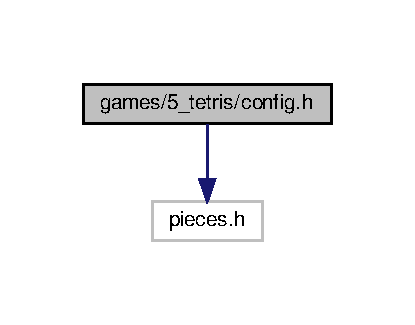
\includegraphics[width=199pt]{5__tetris_2config_8h__incl}
\end{center}
\end{figure}
Ce graphe montre quels fichiers incluent directement ou indirectement ce fichier \+:\nopagebreak
\begin{figure}[H]
\begin{center}
\leavevmode
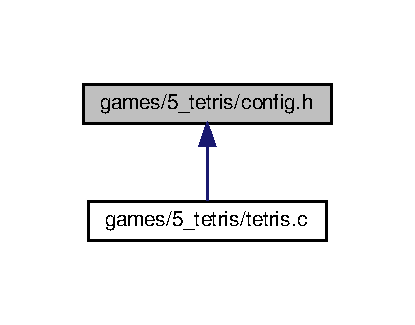
\includegraphics[width=199pt]{5__tetris_2config_8h__dep__incl}
\end{center}
\end{figure}
\subsection*{Structures de données}
\begin{DoxyCompactItemize}
\item 
struct \hyperlink{struct_score}{Score}
\begin{DoxyCompactList}\small\item\em Contient des informations sur les affichages de scores individuels. \end{DoxyCompactList}\item 
struct \hyperlink{struct_score_total}{Score\+Total}
\begin{DoxyCompactList}\small\item\em Contient des informations sur le score total. \end{DoxyCompactList}\item 
struct \hyperlink{struct_piece}{Piece}
\begin{DoxyCompactList}\small\item\em Contient des informations sur une pièce (actuelle ou suivante) \end{DoxyCompactList}\item 
struct \hyperlink{struct_dead_piece}{Dead\+Piece}
\begin{DoxyCompactList}\small\item\em Contient des informations sur les briques lors de l\textquotesingle{}animation de fin de patie. \end{DoxyCompactList}\end{DoxyCompactItemize}
\subsection*{Macros}
\begin{DoxyCompactItemize}
\item 
\#define \hyperlink{5__tetris_2config_8h_a85f9d29551f1bf30f03229da27cb532f}{F\+R\+A\+M\+E\+S\+\_\+\+P\+E\+R\+\_\+\+S\+E\+C\+O\+ND}~30
\item 
\#define \hyperlink{5__tetris_2config_8h_a592bfa81303d4b795563f64ea6c284af}{N\+B\+\_\+\+T\+E\+T\+R\+I\+S\+\_\+\+F\+O\+N\+TS}~1
\item 
\#define \hyperlink{5__tetris_2config_8h_a6282dd398a926253e70a05a4bc933ce2}{N\+B\+\_\+\+T\+E\+T\+R\+I\+S\+\_\+\+S\+O\+U\+N\+DS}~6
\item 
\#define \hyperlink{5__tetris_2config_8h_a2467f25d468ac1b39365c5383b5f17c7}{C\+A\+S\+E\+\_\+\+S\+I\+ZE}~38.
\item 
\#define \hyperlink{5__tetris_2config_8h_ad59c9ac89766941c0861f0afc858abe1}{B\+O\+N\+U\+S\+\_\+\+S\+I\+ZE}~20.
\item 
\#define \hyperlink{5__tetris_2config_8h_a51af8693b7410f0df2a0796abe215160}{G\+R\+I\+L\+L\+E\+\_\+W}~10
\item 
\#define \hyperlink{5__tetris_2config_8h_a5ff40e75231adce782f51f6235c0eb05}{G\+R\+I\+L\+L\+E\+\_\+H}~20
\item 
\#define \hyperlink{5__tetris_2config_8h_ad1690bc13ada14f8c7c8f383d6efa3ac}{F\+R\+A\+M\+E\+\_\+\+C\+O\+M\+P\+L\+E\+T\+E\+\_\+\+L\+I\+NE}~11
\item 
\#define \hyperlink{5__tetris_2config_8h_a2b7cf2a3641be7b89138615764d60ba3}{E\+M\+P\+TY}~-\/1
\item 
\#define \hyperlink{5__tetris_2config_8h_ad0689d356fa051e8b4e47331535f7c92}{F\+R\+A\+M\+E\+\_\+\+R\+E\+M\+I\+N\+D\+\_\+\+R\+O\+T\+A\+TE}~(\hyperlink{7__asteroid_2config_8h_a85f9d29551f1bf30f03229da27cb532f}{F\+R\+A\+M\+E\+S\+\_\+\+P\+E\+R\+\_\+\+S\+E\+C\+O\+ND}/3)
\item 
\#define \hyperlink{5__tetris_2config_8h_ae3b029d68829449045fe31e94da8de72}{R\+O\+U\+N\+D\+A\+B\+LE}~0.\+0001
\item 
\#define \hyperlink{5__tetris_2config_8h_a3bdc3d77ca3e6d7c92b502c91ce81096}{N\+O\+\_\+\+M\+O\+VE}~0
\item 
\#define \hyperlink{5__tetris_2config_8h_a001bb501c43a2caa67dc0d3245bd073c}{M\+O\+V\+E\+\_\+\+R\+I\+G\+HT}~1
\item 
\#define \hyperlink{5__tetris_2config_8h_a4796d02bb619233fee554b3ff9c8da48}{M\+O\+V\+E\+\_\+\+L\+E\+FT}~-\/1
\item 
\#define \hyperlink{5__tetris_2config_8h_a30e9ec8beb81cfa56181bb6068a11517}{T\+O\+O\+\_\+\+C\+L\+O\+S\+E\+\_\+\+F\+R\+O\+M\+\_\+\+T\+OP}~420
\item 
\#define \hyperlink{5__tetris_2config_8h_ae888d76ec9e058aa47eeaaa7917a470d}{S\+T\+O\+P\+P\+ED}~-\/1
\item 
\#define \hyperlink{5__tetris_2config_8h_ad78d742644c2dd6be6786ab38e306d8b}{N\+O\+\_\+\+A\+C\+C\+E\+L\+E\+R\+A\+TE}~1
\item 
\#define \hyperlink{5__tetris_2config_8h_a10a4f38af4f013744abf2d7c6722ef8d}{A\+C\+C\+E\+L\+E\+R\+A\+TE}~10
\item 
\#define \hyperlink{5__tetris_2config_8h_a467e0edbc93466648e5a4efac6a5f36b}{N\+B\+\_\+\+F\+R\+A\+M\+ES}~4
\item 
\#define \hyperlink{5__tetris_2config_8h_a42dccc970b97115fb931fe416e49d0e5}{N\+B\+\_\+\+D\+I\+S\+T\+A\+N\+C\+ES}~2
\item 
\#define \hyperlink{5__tetris_2config_8h_a628b81f81f86e1cb4370883c471a9750}{F\+R\+A\+M\+E\+\_\+\+S\+T\+O\+P\+\_\+\+A\+C\+C\+E\+L\+E\+R\+A\+TE}~1
\item 
\#define \hyperlink{5__tetris_2config_8h_a52916cc9a9b3ff6805728642d63bacd7}{T\+I\+M\+E\+\_\+\+T\+O\+\_\+\+R\+E\+A\+C\+H\+\_\+\+M\+AX}~(\hyperlink{7__asteroid_2config_8h_a85f9d29551f1bf30f03229da27cb532f}{F\+R\+A\+M\+E\+S\+\_\+\+P\+E\+R\+\_\+\+S\+E\+C\+O\+ND}$\ast$60$\ast$7)
\item 
\#define \hyperlink{5__tetris_2config_8h_a478746a56a0f0a831302083552ba2062}{T\+I\+M\+E\+\_\+\+S\+T\+A\+RT}~(\hyperlink{7__asteroid_2config_8h_a85f9d29551f1bf30f03229da27cb532f}{F\+R\+A\+M\+E\+S\+\_\+\+P\+E\+R\+\_\+\+S\+E\+C\+O\+ND}$\ast$60)
\item 
\#define \hyperlink{5__tetris_2config_8h_a8271f0bb542462f1c9f2304605c0434f}{P\+R\+O\+B\+A\+\_\+\+B\+O\+N\+US}~6
\item 
\#define \hyperlink{5__tetris_2config_8h_aa5c414cc45eec8bd806bec316d058444}{N\+B\+\_\+\+B\+O\+N\+U\+S\+ES}~7
\item 
\#define \hyperlink{5__tetris_2config_8h_aee437d1ea74908964820b500978d332f}{B\+O\+N\+U\+S\+\_\+\+T\+RI}~10
\item 
\#define \hyperlink{5__tetris_2config_8h_afb4c1ff0ed702f23663a03857fb07906}{N\+B\+\_\+\+L\+I\+N\+E\+S\+\_\+\+L\+A\+S\+ER}~3
\item 
\#define \hyperlink{5__tetris_2config_8h_a6719afb9c628ab96e4df034e874a6d23}{M\+A\+X\+\_\+\+H\+E\+I\+G\+H\+T\+\_\+\+L\+A\+S\+ER}~13
\item 
\#define \hyperlink{5__tetris_2config_8h_a775b2864209cb216580fc875c9e19a01}{L\+A\+S\+E\+R\+\_\+\+F\+R\+A\+ME}~36
\item 
\#define \hyperlink{5__tetris_2config_8h_a679d48099814d494e410466e07033579}{L\+A\+S\+E\+R\+\_\+\+S\+T\+A\+R\+T\+\_\+\+C\+O\+M\+P\+L\+E\+TE}~22
\item 
\#define \hyperlink{5__tetris_2config_8h_a45729b3f6c165f2eb7c192972499de94}{L\+A\+S\+E\+R\+\_\+\+S\+T\+A\+R\+T\+\_\+\+S\+H\+O\+OT}~28
\item 
\#define \hyperlink{5__tetris_2config_8h_af91e02cf872b55487679fbf7703278f7}{L\+A\+S\+E\+R\+\_\+\+A\+R\+R\+I\+V\+ED}~33
\item 
\#define \hyperlink{5__tetris_2config_8h_aa35695105858eed03a8ed707d5ecbb75}{L\+A\+S\+E\+R\+\_\+\+R\+E\+C\+O\+IL}~23
\item 
\#define \hyperlink{5__tetris_2config_8h_a92d411fd62f7a98183f654c8447ef2da}{L\+A\+S\+E\+R\+\_\+\+R\+E\+C\+O\+I\+L\+\_\+\+D\+U\+R\+A\+T\+I\+ON}~3
\item 
\#define \hyperlink{5__tetris_2config_8h_a76366d5c7ff6999b92bd75d596466db5}{L\+A\+S\+E\+R\+\_\+\+R\+E\+T\+R\+E\+AT}~10
\item 
\#define \hyperlink{5__tetris_2config_8h_a59472e67c96ef9ee60a679efe410f61d}{D\+U\+R\+A\+T\+I\+O\+N\+\_\+\+S\+H\+O\+OT}~14
\item 
\#define \hyperlink{5__tetris_2config_8h_a6c205ae4fe0cfa8fd7c78d083e726fbc}{S\+P\+A\+W\+N\+\_\+\+L\+A\+S\+ER}~(\hyperlink{5__tetris_2config_8h_a67275281efc472b3ab4e2d267262e205}{M\+A\+T\+R\+I\+X\+\_\+X} -\/ 2 $\ast$ \hyperlink{5__tetris_2config_8h_a2467f25d468ac1b39365c5383b5f17c7}{C\+A\+S\+E\+\_\+\+S\+I\+ZE})
\item 
\#define \hyperlink{5__tetris_2config_8h_a52b08321451a69ae7c10be50c8b6f031}{U\+N\+S\+P\+A\+W\+N\+\_\+\+L\+A\+S\+ER}~(\hyperlink{5__tetris_2config_8h_a838674680f981362c9ee60c84d23a010}{I\+N\+N\+E\+R\+\_\+\+L\+E\+FT} -\/ 4 $\ast$ \hyperlink{5__tetris_2config_8h_a2467f25d468ac1b39365c5383b5f17c7}{C\+A\+S\+E\+\_\+\+S\+I\+ZE})
\item 
\#define \hyperlink{5__tetris_2config_8h_afe40045555a90ea5c495af99b278cc02}{L\+A\+S\+E\+R\+\_\+\+E\+N\+D\+\_\+\+P\+OS}~(\hyperlink{5__tetris_2config_8h_a838674680f981362c9ee60c84d23a010}{I\+N\+N\+E\+R\+\_\+\+L\+E\+FT} + 5)
\item 
\#define \hyperlink{5__tetris_2config_8h_aefdda32ab50d939db66f6dab251aaf6a}{S\+L\+O\+W\+\_\+\+A\+M\+M\+O\+U\+NT}~(\hyperlink{7__asteroid_2config_8h_a85f9d29551f1bf30f03229da27cb532f}{F\+R\+A\+M\+E\+S\+\_\+\+P\+E\+R\+\_\+\+S\+E\+C\+O\+ND} $\ast$ 30)
\item 
\#define \hyperlink{5__tetris_2config_8h_ad3298af6db59968e0dd210989a28a001}{S\+P\+E\+E\+D\+\_\+\+A\+M\+M\+O\+U\+NT}~(\hyperlink{7__asteroid_2config_8h_a85f9d29551f1bf30f03229da27cb532f}{F\+R\+A\+M\+E\+S\+\_\+\+P\+E\+R\+\_\+\+S\+E\+C\+O\+ND} $\ast$ 25)
\item 
\#define \hyperlink{5__tetris_2config_8h_ab7bd6a7ccaf84eece22bdd2642e93b96}{N\+B\+\_\+\+F\+I\+LL}~10
\item 
\#define \hyperlink{5__tetris_2config_8h_ac043aa9c7cba979f78d9c2e1fb2da155}{F\+R\+A\+M\+E\+\_\+\+F\+I\+LL}~13
\item 
\#define \hyperlink{5__tetris_2config_8h_a87778a4bfbd03a9e5435148beeded3fc}{E\+S\+P\+A\+C\+E\+M\+E\+N\+T\+\_\+\+F\+R\+A\+M\+E\+\_\+\+F\+I\+LL}~1.\+5
\item 
\#define \hyperlink{5__tetris_2config_8h_acb2cfccbb23cd57c6649b930da824fdf}{F\+R\+A\+M\+E\+\_\+\+D\+E\+P\+L\+A\+C\+E\+M\+E\+N\+T\+\_\+\+F\+I\+LL}~13
\item 
\#define \hyperlink{5__tetris_2config_8h_a8b6f56d7b7d4144867a2efbc5d5799a2}{S\+P\+A\+W\+N\+\_\+\+F\+I\+L\+L\+\_\+X}~(\hyperlink{5__tetris_2config_8h_a838674680f981362c9ee60c84d23a010}{I\+N\+N\+E\+R\+\_\+\+L\+E\+FT} -\/ 2 $\ast$ \hyperlink{5__tetris_2config_8h_a2467f25d468ac1b39365c5383b5f17c7}{C\+A\+S\+E\+\_\+\+S\+I\+ZE})
\item 
\#define \hyperlink{5__tetris_2config_8h_ac93b26aa0cc1f0f53939293f9e773319}{S\+P\+A\+W\+N\+\_\+\+F\+I\+L\+L\+\_\+Y}~(\hyperlink{5__tetris_2config_8h_ae63d1f528c5b8897f52a1b39d4c871b2}{M\+A\+T\+R\+I\+X\+\_\+Y}+(3$\ast$\hyperlink{5__tetris_2config_8h_a5ff40e75231adce782f51f6235c0eb05}{G\+R\+I\+L\+L\+E\+\_\+H}/4)$\ast$\hyperlink{5__tetris_2config_8h_a2467f25d468ac1b39365c5383b5f17c7}{C\+A\+S\+E\+\_\+\+S\+I\+ZE})
\item 
\#define \hyperlink{5__tetris_2config_8h_a3285379994a42725c79cf2876b47ab1c}{S\+C\+O\+R\+E\+\_\+\+B\+A\+SE}~100
\item 
\#define \hyperlink{5__tetris_2config_8h_adabb058ba31e3a56c84e268a39cbf053}{R\+A\+T\+I\+O\+\_\+\+C\+O\+M\+B\+O\+\_\+\+L\+I\+NE}~2
\item 
\#define \hyperlink{5__tetris_2config_8h_aad9700e256509b82640d17cde9c8309c}{N\+B\+\_\+\+F\+L\+A\+T\+\_\+\+P\+O\+I\+NT}~500
\item 
\#define \hyperlink{5__tetris_2config_8h_a65e5b76f5069cd11f9a94b870d33f29f}{R\+A\+T\+I\+O\+\_\+\+M\+U\+L\+T\+I\+\_\+\+P\+O\+I\+NT}~2
\item 
\#define \hyperlink{5__tetris_2config_8h_aaf641c6cea1475fbe57a7be650b3840d}{R\+A\+T\+I\+O\+\_\+\+S\+A\+M\+E\+\_\+\+C\+O\+L\+OR}~10
\item 
\#define \hyperlink{5__tetris_2config_8h_a834e8e3f0149162ffb14d7345be4f47e}{G\+R\+A\+V\+I\+TE}~0.\+2
\item 
\#define \hyperlink{5__tetris_2config_8h_a5cfae711771f649162ca9d0ab0cd29f5}{M\+I\+N\+\_\+\+D\+E\+A\+D\+\_\+\+S\+P\+E\+ED}~-\/50
\item 
\#define \hyperlink{5__tetris_2config_8h_a9c7b069fee3c8184e14a7de8e5da2dc6}{P\+R\+E\+C\+I\+S\+I\+ON}~1000.
\item 
\#define \hyperlink{5__tetris_2config_8h_afcc92c6a9e724441799226f14544be0d}{I\+N\+T\+E\+R\+V\+A\+L\+E\+\_\+\+R\+O\+T\+A\+\_\+\+S\+P\+E\+ED}~(50$\ast$\hyperlink{5__tetris_2config_8h_a9c7b069fee3c8184e14a7de8e5da2dc6}{P\+R\+E\+C\+I\+S\+I\+ON}+1)
\item 
\#define \hyperlink{5__tetris_2config_8h_a2b861d30398a6170c894c30b6d278966}{B\+A\+S\+E\+\_\+\+R\+O\+T\+A\+\_\+\+S\+P\+E\+ED}~-\/25
\item 
\#define \hyperlink{5__tetris_2config_8h_a9d66735aeaa252aec7f8d8c850d4e7c2}{C\+O\+E\+F\+\_\+\+L\+I\+NE}~0.\+2
\item 
\#define \hyperlink{5__tetris_2config_8h_a2a0a2a10343f878434bfdf5e15f6acbe}{M\+I\+N\+\_\+\+R\+O\+TA}~12
\item 
\#define \hyperlink{5__tetris_2config_8h_a67275281efc472b3ab4e2d267262e205}{M\+A\+T\+R\+I\+X\+\_\+X}~(B\+A\+S\+E\+\_\+\+W\+I\+N\+D\+O\+W\+\_\+W/2-\/(\hyperlink{5__tetris_2config_8h_a2467f25d468ac1b39365c5383b5f17c7}{C\+A\+S\+E\+\_\+\+S\+I\+ZE}$\ast$\hyperlink{5__tetris_2config_8h_a51af8693b7410f0df2a0796abe215160}{G\+R\+I\+L\+L\+E\+\_\+W})/2)
\item 
\#define \hyperlink{5__tetris_2config_8h_ae63d1f528c5b8897f52a1b39d4c871b2}{M\+A\+T\+R\+I\+X\+\_\+Y}~(B\+A\+S\+E\+\_\+\+W\+I\+N\+D\+O\+W\+\_\+H/2-\/(\hyperlink{5__tetris_2config_8h_a2467f25d468ac1b39365c5383b5f17c7}{C\+A\+S\+E\+\_\+\+S\+I\+ZE}$\ast$\hyperlink{5__tetris_2config_8h_a5ff40e75231adce782f51f6235c0eb05}{G\+R\+I\+L\+L\+E\+\_\+H})/2)
\item 
\#define \hyperlink{5__tetris_2config_8h_ac3e5b45c4b122756de7f35ee9c5f9caa}{D\+I\+S\+T\+\_\+\+H\+U\+D\+\_\+\+G\+R\+I\+L\+L\+E\+\_\+X}~(77+153+8)
\item 
\#define \hyperlink{5__tetris_2config_8h_a79e521ae004a0b8cc46f672e6e662d63}{D\+I\+S\+T\+\_\+\+H\+U\+D\+\_\+\+G\+R\+I\+L\+L\+E\+\_\+Y}~63
\item 
\#define \hyperlink{5__tetris_2config_8h_a3bc6b6759b5fad089ce4bc593996eba0}{I\+N\+N\+E\+R\+\_\+\+R\+I\+G\+HT}~(H\+U\+D\+\_\+\+G\+R\+I\+L\+L\+E\+\_\+\+D\+I\+M.\+x+684)
\item 
\#define \hyperlink{5__tetris_2config_8h_a838674680f981362c9ee60c84d23a010}{I\+N\+N\+E\+R\+\_\+\+L\+E\+FT}~(H\+U\+D\+\_\+\+G\+R\+I\+L\+L\+E\+\_\+\+D\+I\+M.\+x+196)
\item 
\#define \hyperlink{5__tetris_2config_8h_a372ea138677008b9a947ed4069e97bc6}{S\+H\+I\+F\+T\+\_\+\+R\+I\+G\+H\+T\+\_\+\+N\+E\+XT}~(-\/558-\/8)
\item 
\#define \hyperlink{5__tetris_2config_8h_a0ac6309e69b46478e1ca984a24fe88e6}{S\+H\+I\+F\+T\+\_\+\+T\+O\+P\+\_\+\+N\+E\+XT}~-\/8
\item 
\#define \hyperlink{5__tetris_2config_8h_a1f19735ac01c0aa1b54d6ab5ced0cf9e}{S\+I\+Z\+E\+\_\+\+Q\+U\+IT}~28.
\item 
\#define \hyperlink{5__tetris_2config_8h_ac1f0856ba43e996f698751bb0281695a}{Y\+\_\+\+S\+T\+A\+R\+T\+\_\+\+R\+E\+P\+L\+AY}~(2$\ast$B\+A\+S\+E\+\_\+\+W\+I\+N\+D\+O\+W\+\_\+H/3)
\begin{DoxyCompactList}\small\item\em replay \end{DoxyCompactList}\item 
\#define \hyperlink{5__tetris_2config_8h_a7581d3a5c38c37921ebfbd3fde8b9e50}{N\+B\+\_\+\+H\+E\+LP}~4
\item 
\#define \hyperlink{5__tetris_2config_8h_a06e6b6c6d6888ab20bb04583dcd7d885}{S\+I\+Z\+E\+\_\+\+H\+E\+LP}~32.
\item 
\#define \hyperlink{5__tetris_2config_8h_ad92e1bab26d8c503f8ba60b3cc341be9}{W\+I\+D\+T\+H\+\_\+\+H\+E\+LP}~150
\item 
\#define \hyperlink{5__tetris_2config_8h_a0e5125ad530e207df14ed4137b5305c0}{S\+I\+Z\+E\+\_\+\+H\+E\+L\+P\+\_\+\+B\+O\+N\+US}~28.
\item 
\#define \hyperlink{5__tetris_2config_8h_a3bbf7980441ab3f8c9099e4230cff0aa}{I\+D\+\_\+\+H\+E\+L\+P\+\_\+\+B\+O\+N\+US}~4
\item 
\#define \hyperlink{5__tetris_2config_8h_a59b1b30af5c82398cbb845f09583c4b4}{E\+S\+P\+A\+C\+E\+M\+E\+N\+T\+\_\+\+H\+I\+N\+T\+\_\+\+B\+O\+N\+US}~70
\item 
\#define \hyperlink{5__tetris_2config_8h_af99c267f44d2248418048f76de228d51}{S\+I\+Z\+E\+\_\+\+C\+O\+M\+BO}~(7.$\ast$\hyperlink{5__tetris_2config_8h_a2467f25d468ac1b39365c5383b5f17c7}{C\+A\+S\+E\+\_\+\+S\+I\+ZE}/8)
\item 
\#define \hyperlink{5__tetris_2config_8h_ad02cb8b203938437dd1d161de632caa1}{W\+I\+D\+T\+H\+\_\+\+D\+R\+A\+W\+\_\+\+C\+O\+M\+BO}~630
\item 
\#define \hyperlink{5__tetris_2config_8h_a3bad3489f6aa10fb64e15bddee293bfc}{C\+O\+M\+B\+O\+\_\+\+D\+R\+A\+W\+\_\+X}~(\hyperlink{5__tetris_2config_8h_a67275281efc472b3ab4e2d267262e205}{M\+A\+T\+R\+I\+X\+\_\+X} + \hyperlink{5__tetris_2config_8h_a51af8693b7410f0df2a0796abe215160}{G\+R\+I\+L\+L\+E\+\_\+W} $\ast$ \hyperlink{5__tetris_2config_8h_a2467f25d468ac1b39365c5383b5f17c7}{C\+A\+S\+E\+\_\+\+S\+I\+ZE} + 95)
\item 
\#define \hyperlink{5__tetris_2config_8h_a63c8686f93e6678f6c6c447e5deff53d}{S\+I\+Z\+E\+\_\+\+S\+C\+O\+RE}~25.
\item 
\#define \hyperlink{5__tetris_2config_8h_a0b2edec94de736fdb437353f202c07f6}{S\+I\+Z\+E\+\_\+\+S\+C\+O\+R\+E\+\_\+\+T\+O\+T\+AL}~40.
\item 
\#define \hyperlink{5__tetris_2config_8h_a91957586c56606497d5528a9bd7a915c}{W\+I\+D\+T\+H\+\_\+\+S\+C\+O\+R\+E\+\_\+\+T\+O\+T\+AL}~150
\item 
\#define \hyperlink{5__tetris_2config_8h_a6c9f2388e91c636203c0ac7d7e675899}{S\+C\+O\+R\+E\+\_\+\+T\+TL}~40
\item 
\#define \hyperlink{5__tetris_2config_8h_ac9e215241eed9566001077c8aa236207}{R\+E\+S\+E\+T\+\_\+\+A\+N\+IM}~34
\item 
\#define \hyperlink{5__tetris_2config_8h_a2ac2e991da378cd8941857aeeea1f2f6}{R\+E\+A\+C\+H\+\_\+\+T\+A\+R\+G\+E\+T\+\_\+\+S\+C\+O\+RE}~17
\item 
\#define \hyperlink{5__tetris_2config_8h_a94ec10dfe9732c5de5368d0a04b1844a}{W\+A\+I\+T\+\_\+\+S\+C\+O\+R\+E\+\_\+\+A\+N\+IM}~2
\item 
\#define \hyperlink{5__tetris_2config_8h_afdde5ee34f7e3a12bf31303ddd82d0f8}{F\+O\+N\+T\+\_\+\+H\+E\+I\+G\+H\+T\+\_\+\+R\+A\+T\+IO}~1.\+5
\item 
\#define \hyperlink{5__tetris_2config_8h_a766de6fad7bc336a051d9267ca890092}{M\+A\+X\+\_\+\+A\+P\+P\+E\+N\+D\+\_\+\+L\+E\+N\+G\+HT}~20
\item 
\#define \hyperlink{5__tetris_2config_8h_a6319fc89da4bb99e27aa667213e4392e}{F\+R\+A\+M\+E\+\_\+\+D\+E\+S\+T\+\_\+\+S\+C\+O\+R\+E\+\_\+\+T\+O\+T\+AL}~15
\item 
\#define \hyperlink{5__tetris_2config_8h_a410abaee863d0235957002aebd20565a}{F\+R\+A\+M\+E\+\_\+\+D\+E\+S\+T\+\_\+\+J\+A\+U\+GE}~20
\item 
\#define \hyperlink{5__tetris_2config_8h_a70ed8881b3239899d811215d9c75febe}{L\+A\+S\+E\+R\+\_\+\+W\+I\+D\+TH}~30
\item 
\#define \hyperlink{5__tetris_2config_8h_a959999e640c562f104d25e31946a92fd}{B\+A\+C\+K\+G\+R\+O\+U\+N\+D\+\_\+\+C\+OL}~8
\item 
\#define \hyperlink{5__tetris_2config_8h_a786e68f96945f50342b7e48b1857a0a1}{B\+A\+C\+K\+G\+R\+O\+U\+N\+D\+\_\+\+R\+OW}~10
\item 
\#define \hyperlink{5__tetris_2config_8h_aaad346cf00cb5209f6b0318c4dd24e45}{N\+B\+\_\+\+C\+O\+M\+BO}~8
\end{DoxyCompactItemize}
\subsection*{Énumérations}
\begin{DoxyCompactItemize}
\item 
enum \hyperlink{5__tetris_2config_8h_a95d3172c264d2e03684617fc88363e89}{T\+\_\+\+F\+O\+N\+TS} \{ \hyperlink{2__snake_2config_8h_a95d3172c264d2e03684617fc88363e89af5264f27fa478da40ccabc5924f59945}{S\+\_\+\+B\+A\+S\+E\+\_\+\+F\+O\+NT}, 
\hyperlink{2__snake_2config_8h_a95d3172c264d2e03684617fc88363e89a91d5d5ef298cc29d3c15bc1aac42fa36}{S\+\_\+\+F\+L\+A\+P\+PY}, 
\hyperlink{5__tetris_2config_8h_a95d3172c264d2e03684617fc88363e89aee115797fde6f9637eb4d69dcc52dac6}{T\+\_\+\+F\+O\+N\+T\+\_\+\+C\+O\+M\+BO}
 \}
\item 
enum \{ \newline
\hyperlink{5__tetris_2config_8h_adc29c2ff13d900c2f185ee95427fb06ca479007c793d68387db7d05d6a85a96e0}{S\+O\+U\+N\+D\+\_\+\+L\+I\+NE}, 
\hyperlink{5__tetris_2config_8h_adc29c2ff13d900c2f185ee95427fb06ca1c75cf9740e1222d76d1590635b30bde}{S\+O\+U\+N\+D\+\_\+\+R\+O\+T\+A\+TE}, 
\hyperlink{5__tetris_2config_8h_adc29c2ff13d900c2f185ee95427fb06caad4b76f1b0ba460330eaecbf488ab0b6}{S\+O\+U\+N\+D\+\_\+\+C\+A\+N\+T\+\_\+\+R\+O\+T\+A\+TE}, 
\hyperlink{5__tetris_2config_8h_adc29c2ff13d900c2f185ee95427fb06ca70b644f29fff15e2bb258fb9f4c8c9d0}{S\+O\+U\+N\+D\+\_\+\+H\+IT}, 
\newline
\hyperlink{5__tetris_2config_8h_adc29c2ff13d900c2f185ee95427fb06cab1a87e67db1247dddc5e5288cdf5c0bf}{S\+O\+U\+N\+D\+\_\+\+L\+A\+S\+ER}, 
\hyperlink{5__tetris_2config_8h_adc29c2ff13d900c2f185ee95427fb06ca3c84a26eed13f1442e465fd3b2e64434}{S\+O\+U\+N\+D\+\_\+\+G\+A\+M\+E\+O\+V\+ER}
 \}
\item 
enum \{ \hyperlink{5__tetris_2config_8h_a61dadd085c1777f559549e05962b2c9ea5bc985e4f31d7fba6113ccb4ca466af5}{L\+A\+T\+E\+R\+AL}, 
\hyperlink{5__tetris_2config_8h_a61dadd085c1777f559549e05962b2c9ea9b0b4a95b99523966e0e34ffdadac9da}{D\+O\+WN}, 
\hyperlink{5__tetris_2config_8h_a61dadd085c1777f559549e05962b2c9ea4148879a9f3ac1a7eb165624186a97ba}{T\+O\+\_\+\+GO}, 
\hyperlink{5__tetris_2config_8h_a61dadd085c1777f559549e05962b2c9ea679ee5320d66c8322e310daeb2ee99b8}{S\+T\+OP}
 \}
\item 
enum \{ \newline
\hyperlink{5__tetris_2config_8h_a726ca809ffd3d67ab4b8476646f26635a8b49d99c64f839dd30214157b7582700}{N\+O\+\_\+\+B\+O\+N\+US}, 
\hyperlink{5__tetris_2config_8h_a726ca809ffd3d67ab4b8476646f26635a1d3754a297a681486f8cb3138a27c28b}{F\+I\+LL}, 
\hyperlink{5__tetris_2config_8h_a726ca809ffd3d67ab4b8476646f26635a2e9dfa1d5da5e771b087db2ca9ed77f7}{L\+A\+S\+ER}, 
\hyperlink{5__tetris_2config_8h_a726ca809ffd3d67ab4b8476646f26635a7fc8a9181d1a4165d786646946b6651a}{M\+U\+L\+T\+I\+\_\+\+P\+O\+I\+NT}, 
\newline
\hyperlink{5__tetris_2config_8h_a726ca809ffd3d67ab4b8476646f26635aa15974fe750b770298d4f860a12015cd}{F\+L\+A\+T\+\_\+\+P\+O\+I\+NT}, 
\hyperlink{5__tetris_2config_8h_a726ca809ffd3d67ab4b8476646f26635ab27edad9d3e126dc8448b6030438adb6}{S\+L\+OW}, 
\hyperlink{5__tetris_2config_8h_a726ca809ffd3d67ab4b8476646f26635a1fb3554200c1173d24e97e9d32283ead}{S\+P\+E\+ED}, 
\hyperlink{5__tetris_2config_8h_a726ca809ffd3d67ab4b8476646f26635a91ad8ad206ce7803ea1b7d77f32335e7}{G\+I\+A\+NT}
 \}
\end{DoxyCompactItemize}
\subsection*{Variables}
\begin{DoxyCompactItemize}
\item 
const Vector2f \hyperlink{5__tetris_2config_8h_a347797e32b67d6b32ea2f3155c3fe036}{U\+N\+D\+E\+F\+I\+N\+ED} = \{-\/500, -\/500\}
\item 
char $\ast$ \hyperlink{5__tetris_2config_8h_a015dd4049bcbf6b7b95658876d9f36cf}{D\+I\+R\+\_\+\+F\+O\+N\+T\+S\+\_\+\+T\+E\+T\+R\+IS} \mbox{[}\hyperlink{5__tetris_2config_8h_a592bfa81303d4b795563f64ea6c284af}{N\+B\+\_\+\+T\+E\+T\+R\+I\+S\+\_\+\+F\+O\+N\+TS}\mbox{]}
\item 
char $\ast$ \hyperlink{5__tetris_2config_8h_a9084da3ef5881abe9d5627f854cff64f}{D\+I\+R\+\_\+\+S\+O\+U\+N\+D\+S\+\_\+\+T\+E\+T\+R\+IS} \mbox{[}\hyperlink{5__tetris_2config_8h_a6282dd398a926253e70a05a4bc933ce2}{N\+B\+\_\+\+T\+E\+T\+R\+I\+S\+\_\+\+S\+O\+U\+N\+DS}\mbox{]}
\item 
static int \hyperlink{5__tetris_2config_8h_a8c5a73dcd5565136874278933d48c704}{S\+O\+U\+N\+D\+\_\+\+V\+O\+L\+U\+M\+ES} \mbox{[}\hyperlink{5__tetris_2config_8h_a6282dd398a926253e70a05a4bc933ce2}{N\+B\+\_\+\+T\+E\+T\+R\+I\+S\+\_\+\+S\+O\+U\+N\+DS}\mbox{]} = \{70,128,80,55,113,100\}
\item 
float \hyperlink{5__tetris_2config_8h_a184398f9ac34c77693230aa5529f3bad}{G\+R\+O\+W\+\_\+\+R\+A\+TE} \mbox{[}\hyperlink{5__tetris_2config_8h_a467e0edbc93466648e5a4efac6a5f36b}{N\+B\+\_\+\+F\+R\+A\+M\+ES}\mbox{]} = \{0.\+9999, 0.\+99976, 0.\+9999, 0.\+99988\}
\item 
float \hyperlink{5__tetris_2config_8h_aa7e53785ef9d86453132a25694fad6c8}{F\+R\+A\+M\+E\+\_\+\+S\+T\+A\+RT} \mbox{[}\hyperlink{5__tetris_2config_8h_a467e0edbc93466648e5a4efac6a5f36b}{N\+B\+\_\+\+F\+R\+A\+M\+ES}\mbox{]} = \{6, 13, 15 ,18\}
\item 
float \hyperlink{5__tetris_2config_8h_a3c37ebe65b86d987bbacbfc7e10c0317}{F\+R\+A\+M\+E\+\_\+\+M\+IN} \mbox{[}\hyperlink{5__tetris_2config_8h_a467e0edbc93466648e5a4efac6a5f36b}{N\+B\+\_\+\+F\+R\+A\+M\+ES}\mbox{]} = \{4 , 1, 8, 15\}
\item 
float \hyperlink{5__tetris_2config_8h_ad5c1b3708934b84133db5a846fc9a088}{F\+R\+A\+M\+E\+\_\+\+M\+AX} \mbox{[}\hyperlink{5__tetris_2config_8h_a467e0edbc93466648e5a4efac6a5f36b}{N\+B\+\_\+\+F\+R\+A\+M\+ES}\mbox{]} = \{8, 20, 18, 20\}
\item 
int \hyperlink{5__tetris_2config_8h_abf83a89789a5cc65caf1c1ff8e8c5b34}{L\+A\+S\+E\+R\+\_\+\+R\+E\+C\+O\+I\+L\+\_\+\+D\+I\+ST} \mbox{[}\hyperlink{5__tetris_2config_8h_a92d411fd62f7a98183f654c8447ef2da}{L\+A\+S\+E\+R\+\_\+\+R\+E\+C\+O\+I\+L\+\_\+\+D\+U\+R\+A\+T\+I\+ON}\mbox{]} = \{8,4,2\}
\item 
S\+D\+L\+\_\+\+Point \hyperlink{5__tetris_2config_8h_a64817953577963feaf21d1ceca24ef9f}{I\+N\+T\+E\+R\+V\+A\+L\+E\+\_\+\+D\+E\+A\+D\+\_\+\+S\+P\+E\+ED} = \{14$\ast$\hyperlink{5__tetris_2config_8h_a9c7b069fee3c8184e14a7de8e5da2dc6}{P\+R\+E\+C\+I\+S\+I\+ON}+1,4$\ast$\hyperlink{5__tetris_2config_8h_a9c7b069fee3c8184e14a7de8e5da2dc6}{P\+R\+E\+C\+I\+S\+I\+ON}+1\}
\item 
Vector2f \hyperlink{5__tetris_2config_8h_ade27b175325997524111ad8d4a25ec75}{B\+A\+S\+E\+\_\+\+D\+E\+A\+D\+\_\+\+S\+P\+E\+ED} = \{-\/7, 3\}
\item 
S\+D\+L\+\_\+\+Rect \hyperlink{5__tetris_2config_8h_ade7d0389d9fff06d454e10306eb82f6a}{M\+A\+T\+R\+IX} = \{\hyperlink{5__tetris_2config_8h_a67275281efc472b3ab4e2d267262e205}{M\+A\+T\+R\+I\+X\+\_\+X},\hyperlink{5__tetris_2config_8h_ae63d1f528c5b8897f52a1b39d4c871b2}{M\+A\+T\+R\+I\+X\+\_\+Y},\hyperlink{5__tetris_2config_8h_a51af8693b7410f0df2a0796abe215160}{G\+R\+I\+L\+L\+E\+\_\+W}$\ast$\hyperlink{5__tetris_2config_8h_a2467f25d468ac1b39365c5383b5f17c7}{C\+A\+S\+E\+\_\+\+S\+I\+ZE},\hyperlink{5__tetris_2config_8h_a5ff40e75231adce782f51f6235c0eb05}{G\+R\+I\+L\+L\+E\+\_\+H}$\ast$\hyperlink{5__tetris_2config_8h_a2467f25d468ac1b39365c5383b5f17c7}{C\+A\+S\+E\+\_\+\+S\+I\+ZE} \}
\item 
S\+D\+L\+\_\+\+Rect \hyperlink{5__tetris_2config_8h_acee2135276a60ea7fe296e6fe7eff979}{H\+U\+D\+\_\+\+G\+R\+I\+L\+L\+E\+\_\+\+D\+IM} = \{\hyperlink{5__tetris_2config_8h_a67275281efc472b3ab4e2d267262e205}{M\+A\+T\+R\+I\+X\+\_\+X}-\/\hyperlink{5__tetris_2config_8h_ac3e5b45c4b122756de7f35ee9c5f9caa}{D\+I\+S\+T\+\_\+\+H\+U\+D\+\_\+\+G\+R\+I\+L\+L\+E\+\_\+X} , \hyperlink{5__tetris_2config_8h_ae63d1f528c5b8897f52a1b39d4c871b2}{M\+A\+T\+R\+I\+X\+\_\+Y}-\/\hyperlink{5__tetris_2config_8h_a79e521ae004a0b8cc46f672e6e662d63}{D\+I\+S\+T\+\_\+\+H\+U\+D\+\_\+\+G\+R\+I\+L\+L\+E\+\_\+Y} , 692, 862\}
\item 
char $\ast$ \hyperlink{5__tetris_2config_8h_a84e6cf274c3f2439ef3b1d386dc474c6}{Q\+U\+IT} = \char`\"{}Echap\char`\"{}
\item 
S\+D\+L\+\_\+\+Rect \hyperlink{5__tetris_2config_8h_a05dd6426be20d877029f9fff2f777951}{Q\+U\+I\+T\+\_\+\+D\+E\+ST} = \{20,20,0,0\}
\item 
char $\ast$ \hyperlink{5__tetris_2config_8h_a36728256377dfd56c55773e2292b3fbe}{H\+E\+L\+P\+\_\+\+T\+E\+XT} \mbox{[}\hyperlink{5__tetris_2config_8h_a7581d3a5c38c37921ebfbd3fde8b9e50}{N\+B\+\_\+\+H\+E\+LP}\mbox{]}
\item 
S\+D\+L\+\_\+\+Rect \hyperlink{5__tetris_2config_8h_a0af48e047659a0e513ab4e00c003b0aa}{H\+E\+L\+P\+\_\+\+D\+E\+ST} \mbox{[}\hyperlink{5__tetris_2config_8h_a7581d3a5c38c37921ebfbd3fde8b9e50}{N\+B\+\_\+\+H\+E\+LP}\mbox{]}
\item 
S\+D\+L\+\_\+\+Rect \hyperlink{5__tetris_2config_8h_a2131a805654560bcc80dc5a4785aac43}{F\+L\+E\+C\+H\+E\+\_\+\+S\+RC} = \{0,0, 500, 435\}
\item 
S\+D\+L\+\_\+\+Rect \hyperlink{5__tetris_2config_8h_a3fe63fbd2a85837301200a0173fb968e}{F\+L\+E\+C\+H\+E\+\_\+\+D\+E\+ST} \mbox{[}3\mbox{]}
\item 
S\+D\+L\+\_\+\+Rect \hyperlink{5__tetris_2config_8h_a032941e0cb3f49f634e6daf2bd001225}{T\+U\+R\+N\+\_\+\+S\+RC} = \{0,0, 624, 289\}
\item 
S\+D\+L\+\_\+\+Rect \hyperlink{5__tetris_2config_8h_a33d2885876e61ae0b068abc467eca197}{T\+U\+R\+N\+\_\+\+D\+E\+ST} \mbox{[}2\mbox{]}
\item 
S\+D\+L\+\_\+\+Rect \hyperlink{5__tetris_2config_8h_ae3457d1bf2557211f025cbc93d7ab1db}{B\+O\+N\+U\+S\+\_\+\+H\+I\+N\+T\+\_\+\+D\+E\+ST} = \{80,500,50,30\}
\item 
S\+D\+L\+\_\+\+Rect \hyperlink{5__tetris_2config_8h_ada266e2e551760b22a2699950028187c}{B\+R\+I\+C\+K\+\_\+\+H\+E\+L\+P\+\_\+\+B\+O\+N\+U\+S\+\_\+\+D\+E\+ST} = \{30 ,500, \hyperlink{5__tetris_2config_8h_a2467f25d468ac1b39365c5383b5f17c7}{C\+A\+S\+E\+\_\+\+S\+I\+ZE}, \hyperlink{5__tetris_2config_8h_a2467f25d468ac1b39365c5383b5f17c7}{C\+A\+S\+E\+\_\+\+S\+I\+ZE}\}
\item 
char $\ast$ \hyperlink{5__tetris_2config_8h_ac6a22c854bfd553ff7b22786a7099173}{B\+O\+N\+U\+S\+\_\+\+T\+E\+XT} \mbox{[}\hyperlink{5__tetris_2config_8h_aa5c414cc45eec8bd806bec316d058444}{N\+B\+\_\+\+B\+O\+N\+U\+S\+ES}\mbox{]}
\item 
S\+D\+L\+\_\+\+Rect \hyperlink{5__tetris_2config_8h_afc34df3f934ad7bcc40d08574e93462f}{S\+C\+O\+R\+E\+\_\+\+T\+O\+T\+A\+L\+\_\+\+D\+E\+ST} = \{489+96, 272+54,\hyperlink{5__tetris_2config_8h_a91957586c56606497d5528a9bd7a915c}{W\+I\+D\+T\+H\+\_\+\+S\+C\+O\+R\+E\+\_\+\+T\+O\+T\+AL},\hyperlink{5__tetris_2config_8h_a0b2edec94de736fdb437353f202c07f6}{S\+I\+Z\+E\+\_\+\+S\+C\+O\+R\+E\+\_\+\+T\+O\+T\+AL}\}
\item 
const int \hyperlink{5__tetris_2config_8h_a0b2c1b02146d30afe45524cfe2c447bb}{A\+L\+P\+H\+A\+\_\+\+S\+C\+O\+RE} \mbox{[}\hyperlink{5__tetris_2config_8h_a6c9f2388e91c636203c0ac7d7e675899}{S\+C\+O\+R\+E\+\_\+\+T\+TL}\mbox{]} = \{ 20, 40, 65, 90, 120, 135, 160, 175, 195, 195, 195, 195, 195, 195, 195, 195, 195, 195, 195, 195, 195,195, 195, 195, 195, 195, 195, 195, 195, 195, 195, 195, 195, 175, 145, 110, 90, 70, 40, 20 \}
\item 
S\+D\+L\+\_\+\+Rect \hyperlink{5__tetris_2config_8h_a4e9d87f537ae3e0653817000f1bbde08}{S\+C\+O\+R\+E\+\_\+\+S\+RC} = \{0,0, 12,18\}
\item 
const int \hyperlink{5__tetris_2config_8h_a45fd8e70766a359ab6de02c3c690603a}{S\+C\+O\+R\+E\+\_\+\+D\+E\+ST} = (\hyperlink{5__tetris_2config_8h_a67275281efc472b3ab4e2d267262e205}{M\+A\+T\+R\+I\+X\+\_\+X} + (\hyperlink{5__tetris_2config_8h_a51af8693b7410f0df2a0796abe215160}{G\+R\+I\+L\+L\+E\+\_\+W}-\/0.\+5)/2 $\ast$ \hyperlink{5__tetris_2config_8h_a2467f25d468ac1b39365c5383b5f17c7}{C\+A\+S\+E\+\_\+\+S\+I\+ZE})
\item 
S\+D\+L\+\_\+\+Rect \hyperlink{5__tetris_2config_8h_a76ff6902c3ba9a1c573d3ea31b2ce28b}{J\+A\+U\+G\+E\+\_\+\+S\+P\+E\+E\+D\+\_\+\+D\+E\+ST} = \{\hyperlink{5__tetris_2config_8h_a67275281efc472b3ab4e2d267262e205}{M\+A\+T\+R\+I\+X\+\_\+X}-\/\hyperlink{5__tetris_2config_8h_ac3e5b45c4b122756de7f35ee9c5f9caa}{D\+I\+S\+T\+\_\+\+H\+U\+D\+\_\+\+G\+R\+I\+L\+L\+E\+\_\+X} + 632, \hyperlink{5__tetris_2config_8h_ae63d1f528c5b8897f52a1b39d4c871b2}{M\+A\+T\+R\+I\+X\+\_\+Y}-\/\hyperlink{5__tetris_2config_8h_a79e521ae004a0b8cc46f672e6e662d63}{D\+I\+S\+T\+\_\+\+H\+U\+D\+\_\+\+G\+R\+I\+L\+L\+E\+\_\+Y} + 428, 40 , 402\}
\item 
S\+D\+L\+\_\+\+Rect \hyperlink{5__tetris_2config_8h_ae15e34e7defea64e03dfc4496c2f84eb}{J\+A\+U\+G\+E\+\_\+\+S\+P\+E\+E\+D\+\_\+\+S\+RC} = \{0, 0, 40 , 402\}
\item 
S\+D\+L\+\_\+\+Rect \hyperlink{5__tetris_2config_8h_a821fe18cfc2d66bd510b6f5bfe5a579d}{L\+A\+S\+E\+R\+\_\+\+D\+IM} = \{0,0,500,40\}
\item 
S\+D\+L\+\_\+\+Rect \hyperlink{5__tetris_2config_8h_a504b892640b23ac8b1e43d518339bca0}{B\+R\+I\+C\+K\+\_\+\+S\+RC} = \{0,0,32,32\}
\item 
S\+D\+L\+\_\+\+Rect \hyperlink{5__tetris_2config_8h_a1d2d88ac6ea414594ba7cf27a8f219ac}{B\+R\+I\+C\+K\+\_\+\+D\+E\+ST} = \{0,0, \hyperlink{5__tetris_2config_8h_a2467f25d468ac1b39365c5383b5f17c7}{C\+A\+S\+E\+\_\+\+S\+I\+ZE},\hyperlink{5__tetris_2config_8h_a2467f25d468ac1b39365c5383b5f17c7}{C\+A\+S\+E\+\_\+\+S\+I\+ZE}\}
\item 
S\+D\+L\+\_\+\+Rect \hyperlink{5__tetris_2config_8h_a14ce2a631cb804cdad4b0b0583f3624f}{B\+A\+C\+K\+G\+R\+O\+U\+N\+D\+\_\+\+S\+RC} = \{0,0,960,540\}
\item 
const S\+D\+L\+\_\+\+Color \hyperlink{5__tetris_2config_8h_a77e1d9f083bddf13724102f110ca9d31}{B\+A\+C\+K\+G\+R\+O\+U\+N\+D\+\_\+\+C\+O\+L\+OR} = \{0x00, 0x19, 0x3a\}
\item 
const S\+D\+L\+\_\+\+Color \hyperlink{5__tetris_2config_8h_aba7fc7d52abe9221358dababf70d1a6d}{J\+A\+U\+G\+E\+\_\+\+C\+O\+L\+OR} = \{0x00,0xcc,0x\+F\+F\}
\item 
const S\+D\+L\+\_\+\+Color \hyperlink{5__tetris_2config_8h_ab0238e0ca25079959a64cec1bd041bd2}{J\+A\+U\+G\+E\+\_\+\+C\+O\+L\+O\+R\+\_\+\+B\+A\+C\+K\+G\+R\+O\+U\+ND} = \{0x06,0x1a,0x35\}
\item 
const S\+D\+L\+\_\+\+Color \hyperlink{5__tetris_2config_8h_a511836eda64378a4556a07c4b354a3f4}{C\+O\+N\+T\+O\+U\+R\+\_\+\+G\+R\+I\+L\+LE} = \{0, 51, 94, 255\}
\item 
const S\+D\+L\+\_\+\+Color \hyperlink{5__tetris_2config_8h_a0d87707fca556bfaf7e6868711ada6c1}{C\+O\+R\+P\+S\+\_\+\+G\+R\+I\+L\+LE} = \{0,87,142,255\}
\item 
const S\+D\+L\+\_\+\+Color \hyperlink{5__tetris_2config_8h_a850ffd8650867fbfef2949c2678936c8}{C\+O\+L\+\_\+\+P\+I\+E\+CE} = \{17,108,166,255\}
\item 
const S\+D\+L\+\_\+\+Color \hyperlink{5__tetris_2config_8h_ac5b63a973264c0331522c7ffa8077e0d}{S\+C\+O\+R\+E\+\_\+\+T\+O\+T\+A\+L\+\_\+\+C\+O\+L\+OR} = \{0x7\+D,0x\+F9,0x\+F\+F\}
\item 
const S\+D\+L\+\_\+\+Color \hyperlink{5__tetris_2config_8h_a45c45a5cfe449db31021b5bd8f87d259}{B\+R\+I\+C\+K\+\_\+\+C\+O\+L\+O\+RS} \mbox{[}N\+B\+\_\+\+P\+I\+E\+C\+ES\mbox{]}
\item 
const S\+D\+L\+\_\+\+Color \hyperlink{5__tetris_2config_8h_a1e30025412e4ecfaa48228dc92ee891f}{C\+O\+M\+B\+O\+\_\+\+C\+O\+L\+OR} \mbox{[}\hyperlink{5__tetris_2config_8h_aaad346cf00cb5209f6b0318c4dd24e45}{N\+B\+\_\+\+C\+O\+M\+BO}\mbox{]}
\item 
const S\+D\+L\+\_\+\+Color \hyperlink{5__tetris_2config_8h_a33124fc9b1204c1092f85a1df749a00f}{F\+L\+A\+T\+\_\+\+C\+O\+L\+OR} \mbox{[}\hyperlink{5__tetris_2config_8h_a51af8693b7410f0df2a0796abe215160}{G\+R\+I\+L\+L\+E\+\_\+W}\mbox{]}
\item 
const S\+D\+L\+\_\+\+Color \hyperlink{5__tetris_2config_8h_a7dcf3d0d86259c6bf5e1b8ea422635b2}{M\+U\+L\+T\+I\+\_\+\+C\+O\+L\+OR} \mbox{[}\hyperlink{5__tetris_2config_8h_a51af8693b7410f0df2a0796abe215160}{G\+R\+I\+L\+L\+E\+\_\+W}\mbox{]}
\end{DoxyCompactItemize}


\subsection{Documentation des macros}
\mbox{\Hypertarget{5__tetris_2config_8h_a10a4f38af4f013744abf2d7c6722ef8d}\label{5__tetris_2config_8h_a10a4f38af4f013744abf2d7c6722ef8d}} 
\index{5\+\_\+tetris/config.\+h@{5\+\_\+tetris/config.\+h}!A\+C\+C\+E\+L\+E\+R\+A\+TE@{A\+C\+C\+E\+L\+E\+R\+A\+TE}}
\index{A\+C\+C\+E\+L\+E\+R\+A\+TE@{A\+C\+C\+E\+L\+E\+R\+A\+TE}!5\+\_\+tetris/config.\+h@{5\+\_\+tetris/config.\+h}}
\subsubsection{\texorpdfstring{A\+C\+C\+E\+L\+E\+R\+A\+TE}{ACCELERATE}}
{\footnotesize\ttfamily \#define A\+C\+C\+E\+L\+E\+R\+A\+TE~10}

\mbox{\Hypertarget{5__tetris_2config_8h_a959999e640c562f104d25e31946a92fd}\label{5__tetris_2config_8h_a959999e640c562f104d25e31946a92fd}} 
\index{5\+\_\+tetris/config.\+h@{5\+\_\+tetris/config.\+h}!B\+A\+C\+K\+G\+R\+O\+U\+N\+D\+\_\+\+C\+OL@{B\+A\+C\+K\+G\+R\+O\+U\+N\+D\+\_\+\+C\+OL}}
\index{B\+A\+C\+K\+G\+R\+O\+U\+N\+D\+\_\+\+C\+OL@{B\+A\+C\+K\+G\+R\+O\+U\+N\+D\+\_\+\+C\+OL}!5\+\_\+tetris/config.\+h@{5\+\_\+tetris/config.\+h}}
\subsubsection{\texorpdfstring{B\+A\+C\+K\+G\+R\+O\+U\+N\+D\+\_\+\+C\+OL}{BACKGROUND\_COL}}
{\footnotesize\ttfamily \#define B\+A\+C\+K\+G\+R\+O\+U\+N\+D\+\_\+\+C\+OL~8}

\mbox{\Hypertarget{5__tetris_2config_8h_a786e68f96945f50342b7e48b1857a0a1}\label{5__tetris_2config_8h_a786e68f96945f50342b7e48b1857a0a1}} 
\index{5\+\_\+tetris/config.\+h@{5\+\_\+tetris/config.\+h}!B\+A\+C\+K\+G\+R\+O\+U\+N\+D\+\_\+\+R\+OW@{B\+A\+C\+K\+G\+R\+O\+U\+N\+D\+\_\+\+R\+OW}}
\index{B\+A\+C\+K\+G\+R\+O\+U\+N\+D\+\_\+\+R\+OW@{B\+A\+C\+K\+G\+R\+O\+U\+N\+D\+\_\+\+R\+OW}!5\+\_\+tetris/config.\+h@{5\+\_\+tetris/config.\+h}}
\subsubsection{\texorpdfstring{B\+A\+C\+K\+G\+R\+O\+U\+N\+D\+\_\+\+R\+OW}{BACKGROUND\_ROW}}
{\footnotesize\ttfamily \#define B\+A\+C\+K\+G\+R\+O\+U\+N\+D\+\_\+\+R\+OW~10}

\mbox{\Hypertarget{5__tetris_2config_8h_a2b861d30398a6170c894c30b6d278966}\label{5__tetris_2config_8h_a2b861d30398a6170c894c30b6d278966}} 
\index{5\+\_\+tetris/config.\+h@{5\+\_\+tetris/config.\+h}!B\+A\+S\+E\+\_\+\+R\+O\+T\+A\+\_\+\+S\+P\+E\+ED@{B\+A\+S\+E\+\_\+\+R\+O\+T\+A\+\_\+\+S\+P\+E\+ED}}
\index{B\+A\+S\+E\+\_\+\+R\+O\+T\+A\+\_\+\+S\+P\+E\+ED@{B\+A\+S\+E\+\_\+\+R\+O\+T\+A\+\_\+\+S\+P\+E\+ED}!5\+\_\+tetris/config.\+h@{5\+\_\+tetris/config.\+h}}
\subsubsection{\texorpdfstring{B\+A\+S\+E\+\_\+\+R\+O\+T\+A\+\_\+\+S\+P\+E\+ED}{BASE\_ROTA\_SPEED}}
{\footnotesize\ttfamily \#define B\+A\+S\+E\+\_\+\+R\+O\+T\+A\+\_\+\+S\+P\+E\+ED~-\/25}

\mbox{\Hypertarget{5__tetris_2config_8h_ad59c9ac89766941c0861f0afc858abe1}\label{5__tetris_2config_8h_ad59c9ac89766941c0861f0afc858abe1}} 
\index{5\+\_\+tetris/config.\+h@{5\+\_\+tetris/config.\+h}!B\+O\+N\+U\+S\+\_\+\+S\+I\+ZE@{B\+O\+N\+U\+S\+\_\+\+S\+I\+ZE}}
\index{B\+O\+N\+U\+S\+\_\+\+S\+I\+ZE@{B\+O\+N\+U\+S\+\_\+\+S\+I\+ZE}!5\+\_\+tetris/config.\+h@{5\+\_\+tetris/config.\+h}}
\subsubsection{\texorpdfstring{B\+O\+N\+U\+S\+\_\+\+S\+I\+ZE}{BONUS\_SIZE}}
{\footnotesize\ttfamily \#define B\+O\+N\+U\+S\+\_\+\+S\+I\+ZE~20.}

\mbox{\Hypertarget{5__tetris_2config_8h_aee437d1ea74908964820b500978d332f}\label{5__tetris_2config_8h_aee437d1ea74908964820b500978d332f}} 
\index{5\+\_\+tetris/config.\+h@{5\+\_\+tetris/config.\+h}!B\+O\+N\+U\+S\+\_\+\+T\+RI@{B\+O\+N\+U\+S\+\_\+\+T\+RI}}
\index{B\+O\+N\+U\+S\+\_\+\+T\+RI@{B\+O\+N\+U\+S\+\_\+\+T\+RI}!5\+\_\+tetris/config.\+h@{5\+\_\+tetris/config.\+h}}
\subsubsection{\texorpdfstring{B\+O\+N\+U\+S\+\_\+\+T\+RI}{BONUS\_TRI}}
{\footnotesize\ttfamily \#define B\+O\+N\+U\+S\+\_\+\+T\+RI~10}

\mbox{\Hypertarget{5__tetris_2config_8h_a2467f25d468ac1b39365c5383b5f17c7}\label{5__tetris_2config_8h_a2467f25d468ac1b39365c5383b5f17c7}} 
\index{5\+\_\+tetris/config.\+h@{5\+\_\+tetris/config.\+h}!C\+A\+S\+E\+\_\+\+S\+I\+ZE@{C\+A\+S\+E\+\_\+\+S\+I\+ZE}}
\index{C\+A\+S\+E\+\_\+\+S\+I\+ZE@{C\+A\+S\+E\+\_\+\+S\+I\+ZE}!5\+\_\+tetris/config.\+h@{5\+\_\+tetris/config.\+h}}
\subsubsection{\texorpdfstring{C\+A\+S\+E\+\_\+\+S\+I\+ZE}{CASE\_SIZE}}
{\footnotesize\ttfamily \#define C\+A\+S\+E\+\_\+\+S\+I\+ZE~38.}

\mbox{\Hypertarget{5__tetris_2config_8h_a9d66735aeaa252aec7f8d8c850d4e7c2}\label{5__tetris_2config_8h_a9d66735aeaa252aec7f8d8c850d4e7c2}} 
\index{5\+\_\+tetris/config.\+h@{5\+\_\+tetris/config.\+h}!C\+O\+E\+F\+\_\+\+L\+I\+NE@{C\+O\+E\+F\+\_\+\+L\+I\+NE}}
\index{C\+O\+E\+F\+\_\+\+L\+I\+NE@{C\+O\+E\+F\+\_\+\+L\+I\+NE}!5\+\_\+tetris/config.\+h@{5\+\_\+tetris/config.\+h}}
\subsubsection{\texorpdfstring{C\+O\+E\+F\+\_\+\+L\+I\+NE}{COEF\_LINE}}
{\footnotesize\ttfamily \#define C\+O\+E\+F\+\_\+\+L\+I\+NE~0.\+2}

\mbox{\Hypertarget{5__tetris_2config_8h_a3bad3489f6aa10fb64e15bddee293bfc}\label{5__tetris_2config_8h_a3bad3489f6aa10fb64e15bddee293bfc}} 
\index{5\+\_\+tetris/config.\+h@{5\+\_\+tetris/config.\+h}!C\+O\+M\+B\+O\+\_\+\+D\+R\+A\+W\+\_\+X@{C\+O\+M\+B\+O\+\_\+\+D\+R\+A\+W\+\_\+X}}
\index{C\+O\+M\+B\+O\+\_\+\+D\+R\+A\+W\+\_\+X@{C\+O\+M\+B\+O\+\_\+\+D\+R\+A\+W\+\_\+X}!5\+\_\+tetris/config.\+h@{5\+\_\+tetris/config.\+h}}
\subsubsection{\texorpdfstring{C\+O\+M\+B\+O\+\_\+\+D\+R\+A\+W\+\_\+X}{COMBO\_DRAW\_X}}
{\footnotesize\ttfamily \#define C\+O\+M\+B\+O\+\_\+\+D\+R\+A\+W\+\_\+X~(\hyperlink{5__tetris_2config_8h_a67275281efc472b3ab4e2d267262e205}{M\+A\+T\+R\+I\+X\+\_\+X} + \hyperlink{5__tetris_2config_8h_a51af8693b7410f0df2a0796abe215160}{G\+R\+I\+L\+L\+E\+\_\+W} $\ast$ \hyperlink{5__tetris_2config_8h_a2467f25d468ac1b39365c5383b5f17c7}{C\+A\+S\+E\+\_\+\+S\+I\+ZE} + 95)}

\mbox{\Hypertarget{5__tetris_2config_8h_ac3e5b45c4b122756de7f35ee9c5f9caa}\label{5__tetris_2config_8h_ac3e5b45c4b122756de7f35ee9c5f9caa}} 
\index{5\+\_\+tetris/config.\+h@{5\+\_\+tetris/config.\+h}!D\+I\+S\+T\+\_\+\+H\+U\+D\+\_\+\+G\+R\+I\+L\+L\+E\+\_\+X@{D\+I\+S\+T\+\_\+\+H\+U\+D\+\_\+\+G\+R\+I\+L\+L\+E\+\_\+X}}
\index{D\+I\+S\+T\+\_\+\+H\+U\+D\+\_\+\+G\+R\+I\+L\+L\+E\+\_\+X@{D\+I\+S\+T\+\_\+\+H\+U\+D\+\_\+\+G\+R\+I\+L\+L\+E\+\_\+X}!5\+\_\+tetris/config.\+h@{5\+\_\+tetris/config.\+h}}
\subsubsection{\texorpdfstring{D\+I\+S\+T\+\_\+\+H\+U\+D\+\_\+\+G\+R\+I\+L\+L\+E\+\_\+X}{DIST\_HUD\_GRILLE\_X}}
{\footnotesize\ttfamily \#define D\+I\+S\+T\+\_\+\+H\+U\+D\+\_\+\+G\+R\+I\+L\+L\+E\+\_\+X~(77+153+8)}

\mbox{\Hypertarget{5__tetris_2config_8h_a79e521ae004a0b8cc46f672e6e662d63}\label{5__tetris_2config_8h_a79e521ae004a0b8cc46f672e6e662d63}} 
\index{5\+\_\+tetris/config.\+h@{5\+\_\+tetris/config.\+h}!D\+I\+S\+T\+\_\+\+H\+U\+D\+\_\+\+G\+R\+I\+L\+L\+E\+\_\+Y@{D\+I\+S\+T\+\_\+\+H\+U\+D\+\_\+\+G\+R\+I\+L\+L\+E\+\_\+Y}}
\index{D\+I\+S\+T\+\_\+\+H\+U\+D\+\_\+\+G\+R\+I\+L\+L\+E\+\_\+Y@{D\+I\+S\+T\+\_\+\+H\+U\+D\+\_\+\+G\+R\+I\+L\+L\+E\+\_\+Y}!5\+\_\+tetris/config.\+h@{5\+\_\+tetris/config.\+h}}
\subsubsection{\texorpdfstring{D\+I\+S\+T\+\_\+\+H\+U\+D\+\_\+\+G\+R\+I\+L\+L\+E\+\_\+Y}{DIST\_HUD\_GRILLE\_Y}}
{\footnotesize\ttfamily \#define D\+I\+S\+T\+\_\+\+H\+U\+D\+\_\+\+G\+R\+I\+L\+L\+E\+\_\+Y~63}

\mbox{\Hypertarget{5__tetris_2config_8h_a59472e67c96ef9ee60a679efe410f61d}\label{5__tetris_2config_8h_a59472e67c96ef9ee60a679efe410f61d}} 
\index{5\+\_\+tetris/config.\+h@{5\+\_\+tetris/config.\+h}!D\+U\+R\+A\+T\+I\+O\+N\+\_\+\+S\+H\+O\+OT@{D\+U\+R\+A\+T\+I\+O\+N\+\_\+\+S\+H\+O\+OT}}
\index{D\+U\+R\+A\+T\+I\+O\+N\+\_\+\+S\+H\+O\+OT@{D\+U\+R\+A\+T\+I\+O\+N\+\_\+\+S\+H\+O\+OT}!5\+\_\+tetris/config.\+h@{5\+\_\+tetris/config.\+h}}
\subsubsection{\texorpdfstring{D\+U\+R\+A\+T\+I\+O\+N\+\_\+\+S\+H\+O\+OT}{DURATION\_SHOOT}}
{\footnotesize\ttfamily \#define D\+U\+R\+A\+T\+I\+O\+N\+\_\+\+S\+H\+O\+OT~14}

\mbox{\Hypertarget{5__tetris_2config_8h_a2b7cf2a3641be7b89138615764d60ba3}\label{5__tetris_2config_8h_a2b7cf2a3641be7b89138615764d60ba3}} 
\index{5\+\_\+tetris/config.\+h@{5\+\_\+tetris/config.\+h}!E\+M\+P\+TY@{E\+M\+P\+TY}}
\index{E\+M\+P\+TY@{E\+M\+P\+TY}!5\+\_\+tetris/config.\+h@{5\+\_\+tetris/config.\+h}}
\subsubsection{\texorpdfstring{E\+M\+P\+TY}{EMPTY}}
{\footnotesize\ttfamily \#define E\+M\+P\+TY~-\/1}

\mbox{\Hypertarget{5__tetris_2config_8h_a87778a4bfbd03a9e5435148beeded3fc}\label{5__tetris_2config_8h_a87778a4bfbd03a9e5435148beeded3fc}} 
\index{5\+\_\+tetris/config.\+h@{5\+\_\+tetris/config.\+h}!E\+S\+P\+A\+C\+E\+M\+E\+N\+T\+\_\+\+F\+R\+A\+M\+E\+\_\+\+F\+I\+LL@{E\+S\+P\+A\+C\+E\+M\+E\+N\+T\+\_\+\+F\+R\+A\+M\+E\+\_\+\+F\+I\+LL}}
\index{E\+S\+P\+A\+C\+E\+M\+E\+N\+T\+\_\+\+F\+R\+A\+M\+E\+\_\+\+F\+I\+LL@{E\+S\+P\+A\+C\+E\+M\+E\+N\+T\+\_\+\+F\+R\+A\+M\+E\+\_\+\+F\+I\+LL}!5\+\_\+tetris/config.\+h@{5\+\_\+tetris/config.\+h}}
\subsubsection{\texorpdfstring{E\+S\+P\+A\+C\+E\+M\+E\+N\+T\+\_\+\+F\+R\+A\+M\+E\+\_\+\+F\+I\+LL}{ESPACEMENT\_FRAME\_FILL}}
{\footnotesize\ttfamily \#define E\+S\+P\+A\+C\+E\+M\+E\+N\+T\+\_\+\+F\+R\+A\+M\+E\+\_\+\+F\+I\+LL~1.\+5}

\mbox{\Hypertarget{5__tetris_2config_8h_a59b1b30af5c82398cbb845f09583c4b4}\label{5__tetris_2config_8h_a59b1b30af5c82398cbb845f09583c4b4}} 
\index{5\+\_\+tetris/config.\+h@{5\+\_\+tetris/config.\+h}!E\+S\+P\+A\+C\+E\+M\+E\+N\+T\+\_\+\+H\+I\+N\+T\+\_\+\+B\+O\+N\+US@{E\+S\+P\+A\+C\+E\+M\+E\+N\+T\+\_\+\+H\+I\+N\+T\+\_\+\+B\+O\+N\+US}}
\index{E\+S\+P\+A\+C\+E\+M\+E\+N\+T\+\_\+\+H\+I\+N\+T\+\_\+\+B\+O\+N\+US@{E\+S\+P\+A\+C\+E\+M\+E\+N\+T\+\_\+\+H\+I\+N\+T\+\_\+\+B\+O\+N\+US}!5\+\_\+tetris/config.\+h@{5\+\_\+tetris/config.\+h}}
\subsubsection{\texorpdfstring{E\+S\+P\+A\+C\+E\+M\+E\+N\+T\+\_\+\+H\+I\+N\+T\+\_\+\+B\+O\+N\+US}{ESPACEMENT\_HINT\_BONUS}}
{\footnotesize\ttfamily \#define E\+S\+P\+A\+C\+E\+M\+E\+N\+T\+\_\+\+H\+I\+N\+T\+\_\+\+B\+O\+N\+US~70}

\mbox{\Hypertarget{5__tetris_2config_8h_afdde5ee34f7e3a12bf31303ddd82d0f8}\label{5__tetris_2config_8h_afdde5ee34f7e3a12bf31303ddd82d0f8}} 
\index{5\+\_\+tetris/config.\+h@{5\+\_\+tetris/config.\+h}!F\+O\+N\+T\+\_\+\+H\+E\+I\+G\+H\+T\+\_\+\+R\+A\+T\+IO@{F\+O\+N\+T\+\_\+\+H\+E\+I\+G\+H\+T\+\_\+\+R\+A\+T\+IO}}
\index{F\+O\+N\+T\+\_\+\+H\+E\+I\+G\+H\+T\+\_\+\+R\+A\+T\+IO@{F\+O\+N\+T\+\_\+\+H\+E\+I\+G\+H\+T\+\_\+\+R\+A\+T\+IO}!5\+\_\+tetris/config.\+h@{5\+\_\+tetris/config.\+h}}
\subsubsection{\texorpdfstring{F\+O\+N\+T\+\_\+\+H\+E\+I\+G\+H\+T\+\_\+\+R\+A\+T\+IO}{FONT\_HEIGHT\_RATIO}}
{\footnotesize\ttfamily \#define F\+O\+N\+T\+\_\+\+H\+E\+I\+G\+H\+T\+\_\+\+R\+A\+T\+IO~1.\+5}

\mbox{\Hypertarget{5__tetris_2config_8h_ad1690bc13ada14f8c7c8f383d6efa3ac}\label{5__tetris_2config_8h_ad1690bc13ada14f8c7c8f383d6efa3ac}} 
\index{5\+\_\+tetris/config.\+h@{5\+\_\+tetris/config.\+h}!F\+R\+A\+M\+E\+\_\+\+C\+O\+M\+P\+L\+E\+T\+E\+\_\+\+L\+I\+NE@{F\+R\+A\+M\+E\+\_\+\+C\+O\+M\+P\+L\+E\+T\+E\+\_\+\+L\+I\+NE}}
\index{F\+R\+A\+M\+E\+\_\+\+C\+O\+M\+P\+L\+E\+T\+E\+\_\+\+L\+I\+NE@{F\+R\+A\+M\+E\+\_\+\+C\+O\+M\+P\+L\+E\+T\+E\+\_\+\+L\+I\+NE}!5\+\_\+tetris/config.\+h@{5\+\_\+tetris/config.\+h}}
\subsubsection{\texorpdfstring{F\+R\+A\+M\+E\+\_\+\+C\+O\+M\+P\+L\+E\+T\+E\+\_\+\+L\+I\+NE}{FRAME\_COMPLETE\_LINE}}
{\footnotesize\ttfamily \#define F\+R\+A\+M\+E\+\_\+\+C\+O\+M\+P\+L\+E\+T\+E\+\_\+\+L\+I\+NE~11}

\mbox{\Hypertarget{5__tetris_2config_8h_acb2cfccbb23cd57c6649b930da824fdf}\label{5__tetris_2config_8h_acb2cfccbb23cd57c6649b930da824fdf}} 
\index{5\+\_\+tetris/config.\+h@{5\+\_\+tetris/config.\+h}!F\+R\+A\+M\+E\+\_\+\+D\+E\+P\+L\+A\+C\+E\+M\+E\+N\+T\+\_\+\+F\+I\+LL@{F\+R\+A\+M\+E\+\_\+\+D\+E\+P\+L\+A\+C\+E\+M\+E\+N\+T\+\_\+\+F\+I\+LL}}
\index{F\+R\+A\+M\+E\+\_\+\+D\+E\+P\+L\+A\+C\+E\+M\+E\+N\+T\+\_\+\+F\+I\+LL@{F\+R\+A\+M\+E\+\_\+\+D\+E\+P\+L\+A\+C\+E\+M\+E\+N\+T\+\_\+\+F\+I\+LL}!5\+\_\+tetris/config.\+h@{5\+\_\+tetris/config.\+h}}
\subsubsection{\texorpdfstring{F\+R\+A\+M\+E\+\_\+\+D\+E\+P\+L\+A\+C\+E\+M\+E\+N\+T\+\_\+\+F\+I\+LL}{FRAME\_DEPLACEMENT\_FILL}}
{\footnotesize\ttfamily \#define F\+R\+A\+M\+E\+\_\+\+D\+E\+P\+L\+A\+C\+E\+M\+E\+N\+T\+\_\+\+F\+I\+LL~13}

\mbox{\Hypertarget{5__tetris_2config_8h_a410abaee863d0235957002aebd20565a}\label{5__tetris_2config_8h_a410abaee863d0235957002aebd20565a}} 
\index{5\+\_\+tetris/config.\+h@{5\+\_\+tetris/config.\+h}!F\+R\+A\+M\+E\+\_\+\+D\+E\+S\+T\+\_\+\+J\+A\+U\+GE@{F\+R\+A\+M\+E\+\_\+\+D\+E\+S\+T\+\_\+\+J\+A\+U\+GE}}
\index{F\+R\+A\+M\+E\+\_\+\+D\+E\+S\+T\+\_\+\+J\+A\+U\+GE@{F\+R\+A\+M\+E\+\_\+\+D\+E\+S\+T\+\_\+\+J\+A\+U\+GE}!5\+\_\+tetris/config.\+h@{5\+\_\+tetris/config.\+h}}
\subsubsection{\texorpdfstring{F\+R\+A\+M\+E\+\_\+\+D\+E\+S\+T\+\_\+\+J\+A\+U\+GE}{FRAME\_DEST\_JAUGE}}
{\footnotesize\ttfamily \#define F\+R\+A\+M\+E\+\_\+\+D\+E\+S\+T\+\_\+\+J\+A\+U\+GE~20}

\mbox{\Hypertarget{5__tetris_2config_8h_a6319fc89da4bb99e27aa667213e4392e}\label{5__tetris_2config_8h_a6319fc89da4bb99e27aa667213e4392e}} 
\index{5\+\_\+tetris/config.\+h@{5\+\_\+tetris/config.\+h}!F\+R\+A\+M\+E\+\_\+\+D\+E\+S\+T\+\_\+\+S\+C\+O\+R\+E\+\_\+\+T\+O\+T\+AL@{F\+R\+A\+M\+E\+\_\+\+D\+E\+S\+T\+\_\+\+S\+C\+O\+R\+E\+\_\+\+T\+O\+T\+AL}}
\index{F\+R\+A\+M\+E\+\_\+\+D\+E\+S\+T\+\_\+\+S\+C\+O\+R\+E\+\_\+\+T\+O\+T\+AL@{F\+R\+A\+M\+E\+\_\+\+D\+E\+S\+T\+\_\+\+S\+C\+O\+R\+E\+\_\+\+T\+O\+T\+AL}!5\+\_\+tetris/config.\+h@{5\+\_\+tetris/config.\+h}}
\subsubsection{\texorpdfstring{F\+R\+A\+M\+E\+\_\+\+D\+E\+S\+T\+\_\+\+S\+C\+O\+R\+E\+\_\+\+T\+O\+T\+AL}{FRAME\_DEST\_SCORE\_TOTAL}}
{\footnotesize\ttfamily \#define F\+R\+A\+M\+E\+\_\+\+D\+E\+S\+T\+\_\+\+S\+C\+O\+R\+E\+\_\+\+T\+O\+T\+AL~15}

\mbox{\Hypertarget{5__tetris_2config_8h_ac043aa9c7cba979f78d9c2e1fb2da155}\label{5__tetris_2config_8h_ac043aa9c7cba979f78d9c2e1fb2da155}} 
\index{5\+\_\+tetris/config.\+h@{5\+\_\+tetris/config.\+h}!F\+R\+A\+M\+E\+\_\+\+F\+I\+LL@{F\+R\+A\+M\+E\+\_\+\+F\+I\+LL}}
\index{F\+R\+A\+M\+E\+\_\+\+F\+I\+LL@{F\+R\+A\+M\+E\+\_\+\+F\+I\+LL}!5\+\_\+tetris/config.\+h@{5\+\_\+tetris/config.\+h}}
\subsubsection{\texorpdfstring{F\+R\+A\+M\+E\+\_\+\+F\+I\+LL}{FRAME\_FILL}}
{\footnotesize\ttfamily \#define F\+R\+A\+M\+E\+\_\+\+F\+I\+LL~13}

\mbox{\Hypertarget{5__tetris_2config_8h_ad0689d356fa051e8b4e47331535f7c92}\label{5__tetris_2config_8h_ad0689d356fa051e8b4e47331535f7c92}} 
\index{5\+\_\+tetris/config.\+h@{5\+\_\+tetris/config.\+h}!F\+R\+A\+M\+E\+\_\+\+R\+E\+M\+I\+N\+D\+\_\+\+R\+O\+T\+A\+TE@{F\+R\+A\+M\+E\+\_\+\+R\+E\+M\+I\+N\+D\+\_\+\+R\+O\+T\+A\+TE}}
\index{F\+R\+A\+M\+E\+\_\+\+R\+E\+M\+I\+N\+D\+\_\+\+R\+O\+T\+A\+TE@{F\+R\+A\+M\+E\+\_\+\+R\+E\+M\+I\+N\+D\+\_\+\+R\+O\+T\+A\+TE}!5\+\_\+tetris/config.\+h@{5\+\_\+tetris/config.\+h}}
\subsubsection{\texorpdfstring{F\+R\+A\+M\+E\+\_\+\+R\+E\+M\+I\+N\+D\+\_\+\+R\+O\+T\+A\+TE}{FRAME\_REMIND\_ROTATE}}
{\footnotesize\ttfamily \#define F\+R\+A\+M\+E\+\_\+\+R\+E\+M\+I\+N\+D\+\_\+\+R\+O\+T\+A\+TE~(\hyperlink{7__asteroid_2config_8h_a85f9d29551f1bf30f03229da27cb532f}{F\+R\+A\+M\+E\+S\+\_\+\+P\+E\+R\+\_\+\+S\+E\+C\+O\+ND}/3)}

\mbox{\Hypertarget{5__tetris_2config_8h_a628b81f81f86e1cb4370883c471a9750}\label{5__tetris_2config_8h_a628b81f81f86e1cb4370883c471a9750}} 
\index{5\+\_\+tetris/config.\+h@{5\+\_\+tetris/config.\+h}!F\+R\+A\+M\+E\+\_\+\+S\+T\+O\+P\+\_\+\+A\+C\+C\+E\+L\+E\+R\+A\+TE@{F\+R\+A\+M\+E\+\_\+\+S\+T\+O\+P\+\_\+\+A\+C\+C\+E\+L\+E\+R\+A\+TE}}
\index{F\+R\+A\+M\+E\+\_\+\+S\+T\+O\+P\+\_\+\+A\+C\+C\+E\+L\+E\+R\+A\+TE@{F\+R\+A\+M\+E\+\_\+\+S\+T\+O\+P\+\_\+\+A\+C\+C\+E\+L\+E\+R\+A\+TE}!5\+\_\+tetris/config.\+h@{5\+\_\+tetris/config.\+h}}
\subsubsection{\texorpdfstring{F\+R\+A\+M\+E\+\_\+\+S\+T\+O\+P\+\_\+\+A\+C\+C\+E\+L\+E\+R\+A\+TE}{FRAME\_STOP\_ACCELERATE}}
{\footnotesize\ttfamily \#define F\+R\+A\+M\+E\+\_\+\+S\+T\+O\+P\+\_\+\+A\+C\+C\+E\+L\+E\+R\+A\+TE~1}

\mbox{\Hypertarget{5__tetris_2config_8h_a85f9d29551f1bf30f03229da27cb532f}\label{5__tetris_2config_8h_a85f9d29551f1bf30f03229da27cb532f}} 
\index{5\+\_\+tetris/config.\+h@{5\+\_\+tetris/config.\+h}!F\+R\+A\+M\+E\+S\+\_\+\+P\+E\+R\+\_\+\+S\+E\+C\+O\+ND@{F\+R\+A\+M\+E\+S\+\_\+\+P\+E\+R\+\_\+\+S\+E\+C\+O\+ND}}
\index{F\+R\+A\+M\+E\+S\+\_\+\+P\+E\+R\+\_\+\+S\+E\+C\+O\+ND@{F\+R\+A\+M\+E\+S\+\_\+\+P\+E\+R\+\_\+\+S\+E\+C\+O\+ND}!5\+\_\+tetris/config.\+h@{5\+\_\+tetris/config.\+h}}
\subsubsection{\texorpdfstring{F\+R\+A\+M\+E\+S\+\_\+\+P\+E\+R\+\_\+\+S\+E\+C\+O\+ND}{FRAMES\_PER\_SECOND}}
{\footnotesize\ttfamily \#define F\+R\+A\+M\+E\+S\+\_\+\+P\+E\+R\+\_\+\+S\+E\+C\+O\+ND~30}

\mbox{\Hypertarget{5__tetris_2config_8h_a834e8e3f0149162ffb14d7345be4f47e}\label{5__tetris_2config_8h_a834e8e3f0149162ffb14d7345be4f47e}} 
\index{5\+\_\+tetris/config.\+h@{5\+\_\+tetris/config.\+h}!G\+R\+A\+V\+I\+TE@{G\+R\+A\+V\+I\+TE}}
\index{G\+R\+A\+V\+I\+TE@{G\+R\+A\+V\+I\+TE}!5\+\_\+tetris/config.\+h@{5\+\_\+tetris/config.\+h}}
\subsubsection{\texorpdfstring{G\+R\+A\+V\+I\+TE}{GRAVITE}}
{\footnotesize\ttfamily \#define G\+R\+A\+V\+I\+TE~0.\+2}

\mbox{\Hypertarget{5__tetris_2config_8h_a5ff40e75231adce782f51f6235c0eb05}\label{5__tetris_2config_8h_a5ff40e75231adce782f51f6235c0eb05}} 
\index{5\+\_\+tetris/config.\+h@{5\+\_\+tetris/config.\+h}!G\+R\+I\+L\+L\+E\+\_\+H@{G\+R\+I\+L\+L\+E\+\_\+H}}
\index{G\+R\+I\+L\+L\+E\+\_\+H@{G\+R\+I\+L\+L\+E\+\_\+H}!5\+\_\+tetris/config.\+h@{5\+\_\+tetris/config.\+h}}
\subsubsection{\texorpdfstring{G\+R\+I\+L\+L\+E\+\_\+H}{GRILLE\_H}}
{\footnotesize\ttfamily \#define G\+R\+I\+L\+L\+E\+\_\+H~20}

\mbox{\Hypertarget{5__tetris_2config_8h_a51af8693b7410f0df2a0796abe215160}\label{5__tetris_2config_8h_a51af8693b7410f0df2a0796abe215160}} 
\index{5\+\_\+tetris/config.\+h@{5\+\_\+tetris/config.\+h}!G\+R\+I\+L\+L\+E\+\_\+W@{G\+R\+I\+L\+L\+E\+\_\+W}}
\index{G\+R\+I\+L\+L\+E\+\_\+W@{G\+R\+I\+L\+L\+E\+\_\+W}!5\+\_\+tetris/config.\+h@{5\+\_\+tetris/config.\+h}}
\subsubsection{\texorpdfstring{G\+R\+I\+L\+L\+E\+\_\+W}{GRILLE\_W}}
{\footnotesize\ttfamily \#define G\+R\+I\+L\+L\+E\+\_\+W~10}

\mbox{\Hypertarget{5__tetris_2config_8h_a3bbf7980441ab3f8c9099e4230cff0aa}\label{5__tetris_2config_8h_a3bbf7980441ab3f8c9099e4230cff0aa}} 
\index{5\+\_\+tetris/config.\+h@{5\+\_\+tetris/config.\+h}!I\+D\+\_\+\+H\+E\+L\+P\+\_\+\+B\+O\+N\+US@{I\+D\+\_\+\+H\+E\+L\+P\+\_\+\+B\+O\+N\+US}}
\index{I\+D\+\_\+\+H\+E\+L\+P\+\_\+\+B\+O\+N\+US@{I\+D\+\_\+\+H\+E\+L\+P\+\_\+\+B\+O\+N\+US}!5\+\_\+tetris/config.\+h@{5\+\_\+tetris/config.\+h}}
\subsubsection{\texorpdfstring{I\+D\+\_\+\+H\+E\+L\+P\+\_\+\+B\+O\+N\+US}{ID\_HELP\_BONUS}}
{\footnotesize\ttfamily \#define I\+D\+\_\+\+H\+E\+L\+P\+\_\+\+B\+O\+N\+US~4}

\mbox{\Hypertarget{5__tetris_2config_8h_a838674680f981362c9ee60c84d23a010}\label{5__tetris_2config_8h_a838674680f981362c9ee60c84d23a010}} 
\index{5\+\_\+tetris/config.\+h@{5\+\_\+tetris/config.\+h}!I\+N\+N\+E\+R\+\_\+\+L\+E\+FT@{I\+N\+N\+E\+R\+\_\+\+L\+E\+FT}}
\index{I\+N\+N\+E\+R\+\_\+\+L\+E\+FT@{I\+N\+N\+E\+R\+\_\+\+L\+E\+FT}!5\+\_\+tetris/config.\+h@{5\+\_\+tetris/config.\+h}}
\subsubsection{\texorpdfstring{I\+N\+N\+E\+R\+\_\+\+L\+E\+FT}{INNER\_LEFT}}
{\footnotesize\ttfamily \#define I\+N\+N\+E\+R\+\_\+\+L\+E\+FT~(H\+U\+D\+\_\+\+G\+R\+I\+L\+L\+E\+\_\+\+D\+I\+M.\+x+196)}

\mbox{\Hypertarget{5__tetris_2config_8h_a3bc6b6759b5fad089ce4bc593996eba0}\label{5__tetris_2config_8h_a3bc6b6759b5fad089ce4bc593996eba0}} 
\index{5\+\_\+tetris/config.\+h@{5\+\_\+tetris/config.\+h}!I\+N\+N\+E\+R\+\_\+\+R\+I\+G\+HT@{I\+N\+N\+E\+R\+\_\+\+R\+I\+G\+HT}}
\index{I\+N\+N\+E\+R\+\_\+\+R\+I\+G\+HT@{I\+N\+N\+E\+R\+\_\+\+R\+I\+G\+HT}!5\+\_\+tetris/config.\+h@{5\+\_\+tetris/config.\+h}}
\subsubsection{\texorpdfstring{I\+N\+N\+E\+R\+\_\+\+R\+I\+G\+HT}{INNER\_RIGHT}}
{\footnotesize\ttfamily \#define I\+N\+N\+E\+R\+\_\+\+R\+I\+G\+HT~(H\+U\+D\+\_\+\+G\+R\+I\+L\+L\+E\+\_\+\+D\+I\+M.\+x+684)}

\mbox{\Hypertarget{5__tetris_2config_8h_afcc92c6a9e724441799226f14544be0d}\label{5__tetris_2config_8h_afcc92c6a9e724441799226f14544be0d}} 
\index{5\+\_\+tetris/config.\+h@{5\+\_\+tetris/config.\+h}!I\+N\+T\+E\+R\+V\+A\+L\+E\+\_\+\+R\+O\+T\+A\+\_\+\+S\+P\+E\+ED@{I\+N\+T\+E\+R\+V\+A\+L\+E\+\_\+\+R\+O\+T\+A\+\_\+\+S\+P\+E\+ED}}
\index{I\+N\+T\+E\+R\+V\+A\+L\+E\+\_\+\+R\+O\+T\+A\+\_\+\+S\+P\+E\+ED@{I\+N\+T\+E\+R\+V\+A\+L\+E\+\_\+\+R\+O\+T\+A\+\_\+\+S\+P\+E\+ED}!5\+\_\+tetris/config.\+h@{5\+\_\+tetris/config.\+h}}
\subsubsection{\texorpdfstring{I\+N\+T\+E\+R\+V\+A\+L\+E\+\_\+\+R\+O\+T\+A\+\_\+\+S\+P\+E\+ED}{INTERVALE\_ROTA\_SPEED}}
{\footnotesize\ttfamily \#define I\+N\+T\+E\+R\+V\+A\+L\+E\+\_\+\+R\+O\+T\+A\+\_\+\+S\+P\+E\+ED~(50$\ast$\hyperlink{5__tetris_2config_8h_a9c7b069fee3c8184e14a7de8e5da2dc6}{P\+R\+E\+C\+I\+S\+I\+ON}+1)}

\mbox{\Hypertarget{5__tetris_2config_8h_af91e02cf872b55487679fbf7703278f7}\label{5__tetris_2config_8h_af91e02cf872b55487679fbf7703278f7}} 
\index{5\+\_\+tetris/config.\+h@{5\+\_\+tetris/config.\+h}!L\+A\+S\+E\+R\+\_\+\+A\+R\+R\+I\+V\+ED@{L\+A\+S\+E\+R\+\_\+\+A\+R\+R\+I\+V\+ED}}
\index{L\+A\+S\+E\+R\+\_\+\+A\+R\+R\+I\+V\+ED@{L\+A\+S\+E\+R\+\_\+\+A\+R\+R\+I\+V\+ED}!5\+\_\+tetris/config.\+h@{5\+\_\+tetris/config.\+h}}
\subsubsection{\texorpdfstring{L\+A\+S\+E\+R\+\_\+\+A\+R\+R\+I\+V\+ED}{LASER\_ARRIVED}}
{\footnotesize\ttfamily \#define L\+A\+S\+E\+R\+\_\+\+A\+R\+R\+I\+V\+ED~33}

\mbox{\Hypertarget{5__tetris_2config_8h_afe40045555a90ea5c495af99b278cc02}\label{5__tetris_2config_8h_afe40045555a90ea5c495af99b278cc02}} 
\index{5\+\_\+tetris/config.\+h@{5\+\_\+tetris/config.\+h}!L\+A\+S\+E\+R\+\_\+\+E\+N\+D\+\_\+\+P\+OS@{L\+A\+S\+E\+R\+\_\+\+E\+N\+D\+\_\+\+P\+OS}}
\index{L\+A\+S\+E\+R\+\_\+\+E\+N\+D\+\_\+\+P\+OS@{L\+A\+S\+E\+R\+\_\+\+E\+N\+D\+\_\+\+P\+OS}!5\+\_\+tetris/config.\+h@{5\+\_\+tetris/config.\+h}}
\subsubsection{\texorpdfstring{L\+A\+S\+E\+R\+\_\+\+E\+N\+D\+\_\+\+P\+OS}{LASER\_END\_POS}}
{\footnotesize\ttfamily \#define L\+A\+S\+E\+R\+\_\+\+E\+N\+D\+\_\+\+P\+OS~(\hyperlink{5__tetris_2config_8h_a838674680f981362c9ee60c84d23a010}{I\+N\+N\+E\+R\+\_\+\+L\+E\+FT} + 5)}

\mbox{\Hypertarget{5__tetris_2config_8h_a775b2864209cb216580fc875c9e19a01}\label{5__tetris_2config_8h_a775b2864209cb216580fc875c9e19a01}} 
\index{5\+\_\+tetris/config.\+h@{5\+\_\+tetris/config.\+h}!L\+A\+S\+E\+R\+\_\+\+F\+R\+A\+ME@{L\+A\+S\+E\+R\+\_\+\+F\+R\+A\+ME}}
\index{L\+A\+S\+E\+R\+\_\+\+F\+R\+A\+ME@{L\+A\+S\+E\+R\+\_\+\+F\+R\+A\+ME}!5\+\_\+tetris/config.\+h@{5\+\_\+tetris/config.\+h}}
\subsubsection{\texorpdfstring{L\+A\+S\+E\+R\+\_\+\+F\+R\+A\+ME}{LASER\_FRAME}}
{\footnotesize\ttfamily \#define L\+A\+S\+E\+R\+\_\+\+F\+R\+A\+ME~36}

\mbox{\Hypertarget{5__tetris_2config_8h_aa35695105858eed03a8ed707d5ecbb75}\label{5__tetris_2config_8h_aa35695105858eed03a8ed707d5ecbb75}} 
\index{5\+\_\+tetris/config.\+h@{5\+\_\+tetris/config.\+h}!L\+A\+S\+E\+R\+\_\+\+R\+E\+C\+O\+IL@{L\+A\+S\+E\+R\+\_\+\+R\+E\+C\+O\+IL}}
\index{L\+A\+S\+E\+R\+\_\+\+R\+E\+C\+O\+IL@{L\+A\+S\+E\+R\+\_\+\+R\+E\+C\+O\+IL}!5\+\_\+tetris/config.\+h@{5\+\_\+tetris/config.\+h}}
\subsubsection{\texorpdfstring{L\+A\+S\+E\+R\+\_\+\+R\+E\+C\+O\+IL}{LASER\_RECOIL}}
{\footnotesize\ttfamily \#define L\+A\+S\+E\+R\+\_\+\+R\+E\+C\+O\+IL~23}

\mbox{\Hypertarget{5__tetris_2config_8h_a92d411fd62f7a98183f654c8447ef2da}\label{5__tetris_2config_8h_a92d411fd62f7a98183f654c8447ef2da}} 
\index{5\+\_\+tetris/config.\+h@{5\+\_\+tetris/config.\+h}!L\+A\+S\+E\+R\+\_\+\+R\+E\+C\+O\+I\+L\+\_\+\+D\+U\+R\+A\+T\+I\+ON@{L\+A\+S\+E\+R\+\_\+\+R\+E\+C\+O\+I\+L\+\_\+\+D\+U\+R\+A\+T\+I\+ON}}
\index{L\+A\+S\+E\+R\+\_\+\+R\+E\+C\+O\+I\+L\+\_\+\+D\+U\+R\+A\+T\+I\+ON@{L\+A\+S\+E\+R\+\_\+\+R\+E\+C\+O\+I\+L\+\_\+\+D\+U\+R\+A\+T\+I\+ON}!5\+\_\+tetris/config.\+h@{5\+\_\+tetris/config.\+h}}
\subsubsection{\texorpdfstring{L\+A\+S\+E\+R\+\_\+\+R\+E\+C\+O\+I\+L\+\_\+\+D\+U\+R\+A\+T\+I\+ON}{LASER\_RECOIL\_DURATION}}
{\footnotesize\ttfamily \#define L\+A\+S\+E\+R\+\_\+\+R\+E\+C\+O\+I\+L\+\_\+\+D\+U\+R\+A\+T\+I\+ON~3}

\mbox{\Hypertarget{5__tetris_2config_8h_a76366d5c7ff6999b92bd75d596466db5}\label{5__tetris_2config_8h_a76366d5c7ff6999b92bd75d596466db5}} 
\index{5\+\_\+tetris/config.\+h@{5\+\_\+tetris/config.\+h}!L\+A\+S\+E\+R\+\_\+\+R\+E\+T\+R\+E\+AT@{L\+A\+S\+E\+R\+\_\+\+R\+E\+T\+R\+E\+AT}}
\index{L\+A\+S\+E\+R\+\_\+\+R\+E\+T\+R\+E\+AT@{L\+A\+S\+E\+R\+\_\+\+R\+E\+T\+R\+E\+AT}!5\+\_\+tetris/config.\+h@{5\+\_\+tetris/config.\+h}}
\subsubsection{\texorpdfstring{L\+A\+S\+E\+R\+\_\+\+R\+E\+T\+R\+E\+AT}{LASER\_RETREAT}}
{\footnotesize\ttfamily \#define L\+A\+S\+E\+R\+\_\+\+R\+E\+T\+R\+E\+AT~10}

\mbox{\Hypertarget{5__tetris_2config_8h_a679d48099814d494e410466e07033579}\label{5__tetris_2config_8h_a679d48099814d494e410466e07033579}} 
\index{5\+\_\+tetris/config.\+h@{5\+\_\+tetris/config.\+h}!L\+A\+S\+E\+R\+\_\+\+S\+T\+A\+R\+T\+\_\+\+C\+O\+M\+P\+L\+E\+TE@{L\+A\+S\+E\+R\+\_\+\+S\+T\+A\+R\+T\+\_\+\+C\+O\+M\+P\+L\+E\+TE}}
\index{L\+A\+S\+E\+R\+\_\+\+S\+T\+A\+R\+T\+\_\+\+C\+O\+M\+P\+L\+E\+TE@{L\+A\+S\+E\+R\+\_\+\+S\+T\+A\+R\+T\+\_\+\+C\+O\+M\+P\+L\+E\+TE}!5\+\_\+tetris/config.\+h@{5\+\_\+tetris/config.\+h}}
\subsubsection{\texorpdfstring{L\+A\+S\+E\+R\+\_\+\+S\+T\+A\+R\+T\+\_\+\+C\+O\+M\+P\+L\+E\+TE}{LASER\_START\_COMPLETE}}
{\footnotesize\ttfamily \#define L\+A\+S\+E\+R\+\_\+\+S\+T\+A\+R\+T\+\_\+\+C\+O\+M\+P\+L\+E\+TE~22}

\mbox{\Hypertarget{5__tetris_2config_8h_a45729b3f6c165f2eb7c192972499de94}\label{5__tetris_2config_8h_a45729b3f6c165f2eb7c192972499de94}} 
\index{5\+\_\+tetris/config.\+h@{5\+\_\+tetris/config.\+h}!L\+A\+S\+E\+R\+\_\+\+S\+T\+A\+R\+T\+\_\+\+S\+H\+O\+OT@{L\+A\+S\+E\+R\+\_\+\+S\+T\+A\+R\+T\+\_\+\+S\+H\+O\+OT}}
\index{L\+A\+S\+E\+R\+\_\+\+S\+T\+A\+R\+T\+\_\+\+S\+H\+O\+OT@{L\+A\+S\+E\+R\+\_\+\+S\+T\+A\+R\+T\+\_\+\+S\+H\+O\+OT}!5\+\_\+tetris/config.\+h@{5\+\_\+tetris/config.\+h}}
\subsubsection{\texorpdfstring{L\+A\+S\+E\+R\+\_\+\+S\+T\+A\+R\+T\+\_\+\+S\+H\+O\+OT}{LASER\_START\_SHOOT}}
{\footnotesize\ttfamily \#define L\+A\+S\+E\+R\+\_\+\+S\+T\+A\+R\+T\+\_\+\+S\+H\+O\+OT~28}

\mbox{\Hypertarget{5__tetris_2config_8h_a70ed8881b3239899d811215d9c75febe}\label{5__tetris_2config_8h_a70ed8881b3239899d811215d9c75febe}} 
\index{5\+\_\+tetris/config.\+h@{5\+\_\+tetris/config.\+h}!L\+A\+S\+E\+R\+\_\+\+W\+I\+D\+TH@{L\+A\+S\+E\+R\+\_\+\+W\+I\+D\+TH}}
\index{L\+A\+S\+E\+R\+\_\+\+W\+I\+D\+TH@{L\+A\+S\+E\+R\+\_\+\+W\+I\+D\+TH}!5\+\_\+tetris/config.\+h@{5\+\_\+tetris/config.\+h}}
\subsubsection{\texorpdfstring{L\+A\+S\+E\+R\+\_\+\+W\+I\+D\+TH}{LASER\_WIDTH}}
{\footnotesize\ttfamily \#define L\+A\+S\+E\+R\+\_\+\+W\+I\+D\+TH~30}

\mbox{\Hypertarget{5__tetris_2config_8h_a67275281efc472b3ab4e2d267262e205}\label{5__tetris_2config_8h_a67275281efc472b3ab4e2d267262e205}} 
\index{5\+\_\+tetris/config.\+h@{5\+\_\+tetris/config.\+h}!M\+A\+T\+R\+I\+X\+\_\+X@{M\+A\+T\+R\+I\+X\+\_\+X}}
\index{M\+A\+T\+R\+I\+X\+\_\+X@{M\+A\+T\+R\+I\+X\+\_\+X}!5\+\_\+tetris/config.\+h@{5\+\_\+tetris/config.\+h}}
\subsubsection{\texorpdfstring{M\+A\+T\+R\+I\+X\+\_\+X}{MATRIX\_X}}
{\footnotesize\ttfamily \#define M\+A\+T\+R\+I\+X\+\_\+X~(B\+A\+S\+E\+\_\+\+W\+I\+N\+D\+O\+W\+\_\+W/2-\/(\hyperlink{5__tetris_2config_8h_a2467f25d468ac1b39365c5383b5f17c7}{C\+A\+S\+E\+\_\+\+S\+I\+ZE}$\ast$\hyperlink{5__tetris_2config_8h_a51af8693b7410f0df2a0796abe215160}{G\+R\+I\+L\+L\+E\+\_\+W})/2)}

\mbox{\Hypertarget{5__tetris_2config_8h_ae63d1f528c5b8897f52a1b39d4c871b2}\label{5__tetris_2config_8h_ae63d1f528c5b8897f52a1b39d4c871b2}} 
\index{5\+\_\+tetris/config.\+h@{5\+\_\+tetris/config.\+h}!M\+A\+T\+R\+I\+X\+\_\+Y@{M\+A\+T\+R\+I\+X\+\_\+Y}}
\index{M\+A\+T\+R\+I\+X\+\_\+Y@{M\+A\+T\+R\+I\+X\+\_\+Y}!5\+\_\+tetris/config.\+h@{5\+\_\+tetris/config.\+h}}
\subsubsection{\texorpdfstring{M\+A\+T\+R\+I\+X\+\_\+Y}{MATRIX\_Y}}
{\footnotesize\ttfamily \#define M\+A\+T\+R\+I\+X\+\_\+Y~(B\+A\+S\+E\+\_\+\+W\+I\+N\+D\+O\+W\+\_\+H/2-\/(\hyperlink{5__tetris_2config_8h_a2467f25d468ac1b39365c5383b5f17c7}{C\+A\+S\+E\+\_\+\+S\+I\+ZE}$\ast$\hyperlink{5__tetris_2config_8h_a5ff40e75231adce782f51f6235c0eb05}{G\+R\+I\+L\+L\+E\+\_\+H})/2)}

\mbox{\Hypertarget{5__tetris_2config_8h_a766de6fad7bc336a051d9267ca890092}\label{5__tetris_2config_8h_a766de6fad7bc336a051d9267ca890092}} 
\index{5\+\_\+tetris/config.\+h@{5\+\_\+tetris/config.\+h}!M\+A\+X\+\_\+\+A\+P\+P\+E\+N\+D\+\_\+\+L\+E\+N\+G\+HT@{M\+A\+X\+\_\+\+A\+P\+P\+E\+N\+D\+\_\+\+L\+E\+N\+G\+HT}}
\index{M\+A\+X\+\_\+\+A\+P\+P\+E\+N\+D\+\_\+\+L\+E\+N\+G\+HT@{M\+A\+X\+\_\+\+A\+P\+P\+E\+N\+D\+\_\+\+L\+E\+N\+G\+HT}!5\+\_\+tetris/config.\+h@{5\+\_\+tetris/config.\+h}}
\subsubsection{\texorpdfstring{M\+A\+X\+\_\+\+A\+P\+P\+E\+N\+D\+\_\+\+L\+E\+N\+G\+HT}{MAX\_APPEND\_LENGHT}}
{\footnotesize\ttfamily \#define M\+A\+X\+\_\+\+A\+P\+P\+E\+N\+D\+\_\+\+L\+E\+N\+G\+HT~20}

\mbox{\Hypertarget{5__tetris_2config_8h_a6719afb9c628ab96e4df034e874a6d23}\label{5__tetris_2config_8h_a6719afb9c628ab96e4df034e874a6d23}} 
\index{5\+\_\+tetris/config.\+h@{5\+\_\+tetris/config.\+h}!M\+A\+X\+\_\+\+H\+E\+I\+G\+H\+T\+\_\+\+L\+A\+S\+ER@{M\+A\+X\+\_\+\+H\+E\+I\+G\+H\+T\+\_\+\+L\+A\+S\+ER}}
\index{M\+A\+X\+\_\+\+H\+E\+I\+G\+H\+T\+\_\+\+L\+A\+S\+ER@{M\+A\+X\+\_\+\+H\+E\+I\+G\+H\+T\+\_\+\+L\+A\+S\+ER}!5\+\_\+tetris/config.\+h@{5\+\_\+tetris/config.\+h}}
\subsubsection{\texorpdfstring{M\+A\+X\+\_\+\+H\+E\+I\+G\+H\+T\+\_\+\+L\+A\+S\+ER}{MAX\_HEIGHT\_LASER}}
{\footnotesize\ttfamily \#define M\+A\+X\+\_\+\+H\+E\+I\+G\+H\+T\+\_\+\+L\+A\+S\+ER~13}

\mbox{\Hypertarget{5__tetris_2config_8h_a5cfae711771f649162ca9d0ab0cd29f5}\label{5__tetris_2config_8h_a5cfae711771f649162ca9d0ab0cd29f5}} 
\index{5\+\_\+tetris/config.\+h@{5\+\_\+tetris/config.\+h}!M\+I\+N\+\_\+\+D\+E\+A\+D\+\_\+\+S\+P\+E\+ED@{M\+I\+N\+\_\+\+D\+E\+A\+D\+\_\+\+S\+P\+E\+ED}}
\index{M\+I\+N\+\_\+\+D\+E\+A\+D\+\_\+\+S\+P\+E\+ED@{M\+I\+N\+\_\+\+D\+E\+A\+D\+\_\+\+S\+P\+E\+ED}!5\+\_\+tetris/config.\+h@{5\+\_\+tetris/config.\+h}}
\subsubsection{\texorpdfstring{M\+I\+N\+\_\+\+D\+E\+A\+D\+\_\+\+S\+P\+E\+ED}{MIN\_DEAD\_SPEED}}
{\footnotesize\ttfamily \#define M\+I\+N\+\_\+\+D\+E\+A\+D\+\_\+\+S\+P\+E\+ED~-\/50}

\mbox{\Hypertarget{5__tetris_2config_8h_a2a0a2a10343f878434bfdf5e15f6acbe}\label{5__tetris_2config_8h_a2a0a2a10343f878434bfdf5e15f6acbe}} 
\index{5\+\_\+tetris/config.\+h@{5\+\_\+tetris/config.\+h}!M\+I\+N\+\_\+\+R\+O\+TA@{M\+I\+N\+\_\+\+R\+O\+TA}}
\index{M\+I\+N\+\_\+\+R\+O\+TA@{M\+I\+N\+\_\+\+R\+O\+TA}!5\+\_\+tetris/config.\+h@{5\+\_\+tetris/config.\+h}}
\subsubsection{\texorpdfstring{M\+I\+N\+\_\+\+R\+O\+TA}{MIN\_ROTA}}
{\footnotesize\ttfamily \#define M\+I\+N\+\_\+\+R\+O\+TA~12}

\mbox{\Hypertarget{5__tetris_2config_8h_a4796d02bb619233fee554b3ff9c8da48}\label{5__tetris_2config_8h_a4796d02bb619233fee554b3ff9c8da48}} 
\index{5\+\_\+tetris/config.\+h@{5\+\_\+tetris/config.\+h}!M\+O\+V\+E\+\_\+\+L\+E\+FT@{M\+O\+V\+E\+\_\+\+L\+E\+FT}}
\index{M\+O\+V\+E\+\_\+\+L\+E\+FT@{M\+O\+V\+E\+\_\+\+L\+E\+FT}!5\+\_\+tetris/config.\+h@{5\+\_\+tetris/config.\+h}}
\subsubsection{\texorpdfstring{M\+O\+V\+E\+\_\+\+L\+E\+FT}{MOVE\_LEFT}}
{\footnotesize\ttfamily \#define M\+O\+V\+E\+\_\+\+L\+E\+FT~-\/1}

\mbox{\Hypertarget{5__tetris_2config_8h_a001bb501c43a2caa67dc0d3245bd073c}\label{5__tetris_2config_8h_a001bb501c43a2caa67dc0d3245bd073c}} 
\index{5\+\_\+tetris/config.\+h@{5\+\_\+tetris/config.\+h}!M\+O\+V\+E\+\_\+\+R\+I\+G\+HT@{M\+O\+V\+E\+\_\+\+R\+I\+G\+HT}}
\index{M\+O\+V\+E\+\_\+\+R\+I\+G\+HT@{M\+O\+V\+E\+\_\+\+R\+I\+G\+HT}!5\+\_\+tetris/config.\+h@{5\+\_\+tetris/config.\+h}}
\subsubsection{\texorpdfstring{M\+O\+V\+E\+\_\+\+R\+I\+G\+HT}{MOVE\_RIGHT}}
{\footnotesize\ttfamily \#define M\+O\+V\+E\+\_\+\+R\+I\+G\+HT~1}

\mbox{\Hypertarget{5__tetris_2config_8h_aa5c414cc45eec8bd806bec316d058444}\label{5__tetris_2config_8h_aa5c414cc45eec8bd806bec316d058444}} 
\index{5\+\_\+tetris/config.\+h@{5\+\_\+tetris/config.\+h}!N\+B\+\_\+\+B\+O\+N\+U\+S\+ES@{N\+B\+\_\+\+B\+O\+N\+U\+S\+ES}}
\index{N\+B\+\_\+\+B\+O\+N\+U\+S\+ES@{N\+B\+\_\+\+B\+O\+N\+U\+S\+ES}!5\+\_\+tetris/config.\+h@{5\+\_\+tetris/config.\+h}}
\subsubsection{\texorpdfstring{N\+B\+\_\+\+B\+O\+N\+U\+S\+ES}{NB\_BONUSES}}
{\footnotesize\ttfamily \#define N\+B\+\_\+\+B\+O\+N\+U\+S\+ES~7}

\mbox{\Hypertarget{5__tetris_2config_8h_aaad346cf00cb5209f6b0318c4dd24e45}\label{5__tetris_2config_8h_aaad346cf00cb5209f6b0318c4dd24e45}} 
\index{5\+\_\+tetris/config.\+h@{5\+\_\+tetris/config.\+h}!N\+B\+\_\+\+C\+O\+M\+BO@{N\+B\+\_\+\+C\+O\+M\+BO}}
\index{N\+B\+\_\+\+C\+O\+M\+BO@{N\+B\+\_\+\+C\+O\+M\+BO}!5\+\_\+tetris/config.\+h@{5\+\_\+tetris/config.\+h}}
\subsubsection{\texorpdfstring{N\+B\+\_\+\+C\+O\+M\+BO}{NB\_COMBO}}
{\footnotesize\ttfamily \#define N\+B\+\_\+\+C\+O\+M\+BO~8}

\mbox{\Hypertarget{5__tetris_2config_8h_a42dccc970b97115fb931fe416e49d0e5}\label{5__tetris_2config_8h_a42dccc970b97115fb931fe416e49d0e5}} 
\index{5\+\_\+tetris/config.\+h@{5\+\_\+tetris/config.\+h}!N\+B\+\_\+\+D\+I\+S\+T\+A\+N\+C\+ES@{N\+B\+\_\+\+D\+I\+S\+T\+A\+N\+C\+ES}}
\index{N\+B\+\_\+\+D\+I\+S\+T\+A\+N\+C\+ES@{N\+B\+\_\+\+D\+I\+S\+T\+A\+N\+C\+ES}!5\+\_\+tetris/config.\+h@{5\+\_\+tetris/config.\+h}}
\subsubsection{\texorpdfstring{N\+B\+\_\+\+D\+I\+S\+T\+A\+N\+C\+ES}{NB\_DISTANCES}}
{\footnotesize\ttfamily \#define N\+B\+\_\+\+D\+I\+S\+T\+A\+N\+C\+ES~2}

\mbox{\Hypertarget{5__tetris_2config_8h_ab7bd6a7ccaf84eece22bdd2642e93b96}\label{5__tetris_2config_8h_ab7bd6a7ccaf84eece22bdd2642e93b96}} 
\index{5\+\_\+tetris/config.\+h@{5\+\_\+tetris/config.\+h}!N\+B\+\_\+\+F\+I\+LL@{N\+B\+\_\+\+F\+I\+LL}}
\index{N\+B\+\_\+\+F\+I\+LL@{N\+B\+\_\+\+F\+I\+LL}!5\+\_\+tetris/config.\+h@{5\+\_\+tetris/config.\+h}}
\subsubsection{\texorpdfstring{N\+B\+\_\+\+F\+I\+LL}{NB\_FILL}}
{\footnotesize\ttfamily \#define N\+B\+\_\+\+F\+I\+LL~10}

\mbox{\Hypertarget{5__tetris_2config_8h_aad9700e256509b82640d17cde9c8309c}\label{5__tetris_2config_8h_aad9700e256509b82640d17cde9c8309c}} 
\index{5\+\_\+tetris/config.\+h@{5\+\_\+tetris/config.\+h}!N\+B\+\_\+\+F\+L\+A\+T\+\_\+\+P\+O\+I\+NT@{N\+B\+\_\+\+F\+L\+A\+T\+\_\+\+P\+O\+I\+NT}}
\index{N\+B\+\_\+\+F\+L\+A\+T\+\_\+\+P\+O\+I\+NT@{N\+B\+\_\+\+F\+L\+A\+T\+\_\+\+P\+O\+I\+NT}!5\+\_\+tetris/config.\+h@{5\+\_\+tetris/config.\+h}}
\subsubsection{\texorpdfstring{N\+B\+\_\+\+F\+L\+A\+T\+\_\+\+P\+O\+I\+NT}{NB\_FLAT\_POINT}}
{\footnotesize\ttfamily \#define N\+B\+\_\+\+F\+L\+A\+T\+\_\+\+P\+O\+I\+NT~500}

\mbox{\Hypertarget{5__tetris_2config_8h_a467e0edbc93466648e5a4efac6a5f36b}\label{5__tetris_2config_8h_a467e0edbc93466648e5a4efac6a5f36b}} 
\index{5\+\_\+tetris/config.\+h@{5\+\_\+tetris/config.\+h}!N\+B\+\_\+\+F\+R\+A\+M\+ES@{N\+B\+\_\+\+F\+R\+A\+M\+ES}}
\index{N\+B\+\_\+\+F\+R\+A\+M\+ES@{N\+B\+\_\+\+F\+R\+A\+M\+ES}!5\+\_\+tetris/config.\+h@{5\+\_\+tetris/config.\+h}}
\subsubsection{\texorpdfstring{N\+B\+\_\+\+F\+R\+A\+M\+ES}{NB\_FRAMES}}
{\footnotesize\ttfamily \#define N\+B\+\_\+\+F\+R\+A\+M\+ES~4}

\mbox{\Hypertarget{5__tetris_2config_8h_a7581d3a5c38c37921ebfbd3fde8b9e50}\label{5__tetris_2config_8h_a7581d3a5c38c37921ebfbd3fde8b9e50}} 
\index{5\+\_\+tetris/config.\+h@{5\+\_\+tetris/config.\+h}!N\+B\+\_\+\+H\+E\+LP@{N\+B\+\_\+\+H\+E\+LP}}
\index{N\+B\+\_\+\+H\+E\+LP@{N\+B\+\_\+\+H\+E\+LP}!5\+\_\+tetris/config.\+h@{5\+\_\+tetris/config.\+h}}
\subsubsection{\texorpdfstring{N\+B\+\_\+\+H\+E\+LP}{NB\_HELP}}
{\footnotesize\ttfamily \#define N\+B\+\_\+\+H\+E\+LP~4}

\mbox{\Hypertarget{5__tetris_2config_8h_afb4c1ff0ed702f23663a03857fb07906}\label{5__tetris_2config_8h_afb4c1ff0ed702f23663a03857fb07906}} 
\index{5\+\_\+tetris/config.\+h@{5\+\_\+tetris/config.\+h}!N\+B\+\_\+\+L\+I\+N\+E\+S\+\_\+\+L\+A\+S\+ER@{N\+B\+\_\+\+L\+I\+N\+E\+S\+\_\+\+L\+A\+S\+ER}}
\index{N\+B\+\_\+\+L\+I\+N\+E\+S\+\_\+\+L\+A\+S\+ER@{N\+B\+\_\+\+L\+I\+N\+E\+S\+\_\+\+L\+A\+S\+ER}!5\+\_\+tetris/config.\+h@{5\+\_\+tetris/config.\+h}}
\subsubsection{\texorpdfstring{N\+B\+\_\+\+L\+I\+N\+E\+S\+\_\+\+L\+A\+S\+ER}{NB\_LINES\_LASER}}
{\footnotesize\ttfamily \#define N\+B\+\_\+\+L\+I\+N\+E\+S\+\_\+\+L\+A\+S\+ER~3}

\mbox{\Hypertarget{5__tetris_2config_8h_a592bfa81303d4b795563f64ea6c284af}\label{5__tetris_2config_8h_a592bfa81303d4b795563f64ea6c284af}} 
\index{5\+\_\+tetris/config.\+h@{5\+\_\+tetris/config.\+h}!N\+B\+\_\+\+T\+E\+T\+R\+I\+S\+\_\+\+F\+O\+N\+TS@{N\+B\+\_\+\+T\+E\+T\+R\+I\+S\+\_\+\+F\+O\+N\+TS}}
\index{N\+B\+\_\+\+T\+E\+T\+R\+I\+S\+\_\+\+F\+O\+N\+TS@{N\+B\+\_\+\+T\+E\+T\+R\+I\+S\+\_\+\+F\+O\+N\+TS}!5\+\_\+tetris/config.\+h@{5\+\_\+tetris/config.\+h}}
\subsubsection{\texorpdfstring{N\+B\+\_\+\+T\+E\+T\+R\+I\+S\+\_\+\+F\+O\+N\+TS}{NB\_TETRIS\_FONTS}}
{\footnotesize\ttfamily \#define N\+B\+\_\+\+T\+E\+T\+R\+I\+S\+\_\+\+F\+O\+N\+TS~1}

\mbox{\Hypertarget{5__tetris_2config_8h_a6282dd398a926253e70a05a4bc933ce2}\label{5__tetris_2config_8h_a6282dd398a926253e70a05a4bc933ce2}} 
\index{5\+\_\+tetris/config.\+h@{5\+\_\+tetris/config.\+h}!N\+B\+\_\+\+T\+E\+T\+R\+I\+S\+\_\+\+S\+O\+U\+N\+DS@{N\+B\+\_\+\+T\+E\+T\+R\+I\+S\+\_\+\+S\+O\+U\+N\+DS}}
\index{N\+B\+\_\+\+T\+E\+T\+R\+I\+S\+\_\+\+S\+O\+U\+N\+DS@{N\+B\+\_\+\+T\+E\+T\+R\+I\+S\+\_\+\+S\+O\+U\+N\+DS}!5\+\_\+tetris/config.\+h@{5\+\_\+tetris/config.\+h}}
\subsubsection{\texorpdfstring{N\+B\+\_\+\+T\+E\+T\+R\+I\+S\+\_\+\+S\+O\+U\+N\+DS}{NB\_TETRIS\_SOUNDS}}
{\footnotesize\ttfamily \#define N\+B\+\_\+\+T\+E\+T\+R\+I\+S\+\_\+\+S\+O\+U\+N\+DS~6}

\mbox{\Hypertarget{5__tetris_2config_8h_ad78d742644c2dd6be6786ab38e306d8b}\label{5__tetris_2config_8h_ad78d742644c2dd6be6786ab38e306d8b}} 
\index{5\+\_\+tetris/config.\+h@{5\+\_\+tetris/config.\+h}!N\+O\+\_\+\+A\+C\+C\+E\+L\+E\+R\+A\+TE@{N\+O\+\_\+\+A\+C\+C\+E\+L\+E\+R\+A\+TE}}
\index{N\+O\+\_\+\+A\+C\+C\+E\+L\+E\+R\+A\+TE@{N\+O\+\_\+\+A\+C\+C\+E\+L\+E\+R\+A\+TE}!5\+\_\+tetris/config.\+h@{5\+\_\+tetris/config.\+h}}
\subsubsection{\texorpdfstring{N\+O\+\_\+\+A\+C\+C\+E\+L\+E\+R\+A\+TE}{NO\_ACCELERATE}}
{\footnotesize\ttfamily \#define N\+O\+\_\+\+A\+C\+C\+E\+L\+E\+R\+A\+TE~1}

\mbox{\Hypertarget{5__tetris_2config_8h_a3bdc3d77ca3e6d7c92b502c91ce81096}\label{5__tetris_2config_8h_a3bdc3d77ca3e6d7c92b502c91ce81096}} 
\index{5\+\_\+tetris/config.\+h@{5\+\_\+tetris/config.\+h}!N\+O\+\_\+\+M\+O\+VE@{N\+O\+\_\+\+M\+O\+VE}}
\index{N\+O\+\_\+\+M\+O\+VE@{N\+O\+\_\+\+M\+O\+VE}!5\+\_\+tetris/config.\+h@{5\+\_\+tetris/config.\+h}}
\subsubsection{\texorpdfstring{N\+O\+\_\+\+M\+O\+VE}{NO\_MOVE}}
{\footnotesize\ttfamily \#define N\+O\+\_\+\+M\+O\+VE~0}

\mbox{\Hypertarget{5__tetris_2config_8h_a9c7b069fee3c8184e14a7de8e5da2dc6}\label{5__tetris_2config_8h_a9c7b069fee3c8184e14a7de8e5da2dc6}} 
\index{5\+\_\+tetris/config.\+h@{5\+\_\+tetris/config.\+h}!P\+R\+E\+C\+I\+S\+I\+ON@{P\+R\+E\+C\+I\+S\+I\+ON}}
\index{P\+R\+E\+C\+I\+S\+I\+ON@{P\+R\+E\+C\+I\+S\+I\+ON}!5\+\_\+tetris/config.\+h@{5\+\_\+tetris/config.\+h}}
\subsubsection{\texorpdfstring{P\+R\+E\+C\+I\+S\+I\+ON}{PRECISION}}
{\footnotesize\ttfamily \#define P\+R\+E\+C\+I\+S\+I\+ON~1000.}

\mbox{\Hypertarget{5__tetris_2config_8h_a8271f0bb542462f1c9f2304605c0434f}\label{5__tetris_2config_8h_a8271f0bb542462f1c9f2304605c0434f}} 
\index{5\+\_\+tetris/config.\+h@{5\+\_\+tetris/config.\+h}!P\+R\+O\+B\+A\+\_\+\+B\+O\+N\+US@{P\+R\+O\+B\+A\+\_\+\+B\+O\+N\+US}}
\index{P\+R\+O\+B\+A\+\_\+\+B\+O\+N\+US@{P\+R\+O\+B\+A\+\_\+\+B\+O\+N\+US}!5\+\_\+tetris/config.\+h@{5\+\_\+tetris/config.\+h}}
\subsubsection{\texorpdfstring{P\+R\+O\+B\+A\+\_\+\+B\+O\+N\+US}{PROBA\_BONUS}}
{\footnotesize\ttfamily \#define P\+R\+O\+B\+A\+\_\+\+B\+O\+N\+US~6}

\mbox{\Hypertarget{5__tetris_2config_8h_adabb058ba31e3a56c84e268a39cbf053}\label{5__tetris_2config_8h_adabb058ba31e3a56c84e268a39cbf053}} 
\index{5\+\_\+tetris/config.\+h@{5\+\_\+tetris/config.\+h}!R\+A\+T\+I\+O\+\_\+\+C\+O\+M\+B\+O\+\_\+\+L\+I\+NE@{R\+A\+T\+I\+O\+\_\+\+C\+O\+M\+B\+O\+\_\+\+L\+I\+NE}}
\index{R\+A\+T\+I\+O\+\_\+\+C\+O\+M\+B\+O\+\_\+\+L\+I\+NE@{R\+A\+T\+I\+O\+\_\+\+C\+O\+M\+B\+O\+\_\+\+L\+I\+NE}!5\+\_\+tetris/config.\+h@{5\+\_\+tetris/config.\+h}}
\subsubsection{\texorpdfstring{R\+A\+T\+I\+O\+\_\+\+C\+O\+M\+B\+O\+\_\+\+L\+I\+NE}{RATIO\_COMBO\_LINE}}
{\footnotesize\ttfamily \#define R\+A\+T\+I\+O\+\_\+\+C\+O\+M\+B\+O\+\_\+\+L\+I\+NE~2}

\mbox{\Hypertarget{5__tetris_2config_8h_a65e5b76f5069cd11f9a94b870d33f29f}\label{5__tetris_2config_8h_a65e5b76f5069cd11f9a94b870d33f29f}} 
\index{5\+\_\+tetris/config.\+h@{5\+\_\+tetris/config.\+h}!R\+A\+T\+I\+O\+\_\+\+M\+U\+L\+T\+I\+\_\+\+P\+O\+I\+NT@{R\+A\+T\+I\+O\+\_\+\+M\+U\+L\+T\+I\+\_\+\+P\+O\+I\+NT}}
\index{R\+A\+T\+I\+O\+\_\+\+M\+U\+L\+T\+I\+\_\+\+P\+O\+I\+NT@{R\+A\+T\+I\+O\+\_\+\+M\+U\+L\+T\+I\+\_\+\+P\+O\+I\+NT}!5\+\_\+tetris/config.\+h@{5\+\_\+tetris/config.\+h}}
\subsubsection{\texorpdfstring{R\+A\+T\+I\+O\+\_\+\+M\+U\+L\+T\+I\+\_\+\+P\+O\+I\+NT}{RATIO\_MULTI\_POINT}}
{\footnotesize\ttfamily \#define R\+A\+T\+I\+O\+\_\+\+M\+U\+L\+T\+I\+\_\+\+P\+O\+I\+NT~2}

\mbox{\Hypertarget{5__tetris_2config_8h_aaf641c6cea1475fbe57a7be650b3840d}\label{5__tetris_2config_8h_aaf641c6cea1475fbe57a7be650b3840d}} 
\index{5\+\_\+tetris/config.\+h@{5\+\_\+tetris/config.\+h}!R\+A\+T\+I\+O\+\_\+\+S\+A\+M\+E\+\_\+\+C\+O\+L\+OR@{R\+A\+T\+I\+O\+\_\+\+S\+A\+M\+E\+\_\+\+C\+O\+L\+OR}}
\index{R\+A\+T\+I\+O\+\_\+\+S\+A\+M\+E\+\_\+\+C\+O\+L\+OR@{R\+A\+T\+I\+O\+\_\+\+S\+A\+M\+E\+\_\+\+C\+O\+L\+OR}!5\+\_\+tetris/config.\+h@{5\+\_\+tetris/config.\+h}}
\subsubsection{\texorpdfstring{R\+A\+T\+I\+O\+\_\+\+S\+A\+M\+E\+\_\+\+C\+O\+L\+OR}{RATIO\_SAME\_COLOR}}
{\footnotesize\ttfamily \#define R\+A\+T\+I\+O\+\_\+\+S\+A\+M\+E\+\_\+\+C\+O\+L\+OR~10}

\mbox{\Hypertarget{5__tetris_2config_8h_a2ac2e991da378cd8941857aeeea1f2f6}\label{5__tetris_2config_8h_a2ac2e991da378cd8941857aeeea1f2f6}} 
\index{5\+\_\+tetris/config.\+h@{5\+\_\+tetris/config.\+h}!R\+E\+A\+C\+H\+\_\+\+T\+A\+R\+G\+E\+T\+\_\+\+S\+C\+O\+RE@{R\+E\+A\+C\+H\+\_\+\+T\+A\+R\+G\+E\+T\+\_\+\+S\+C\+O\+RE}}
\index{R\+E\+A\+C\+H\+\_\+\+T\+A\+R\+G\+E\+T\+\_\+\+S\+C\+O\+RE@{R\+E\+A\+C\+H\+\_\+\+T\+A\+R\+G\+E\+T\+\_\+\+S\+C\+O\+RE}!5\+\_\+tetris/config.\+h@{5\+\_\+tetris/config.\+h}}
\subsubsection{\texorpdfstring{R\+E\+A\+C\+H\+\_\+\+T\+A\+R\+G\+E\+T\+\_\+\+S\+C\+O\+RE}{REACH\_TARGET\_SCORE}}
{\footnotesize\ttfamily \#define R\+E\+A\+C\+H\+\_\+\+T\+A\+R\+G\+E\+T\+\_\+\+S\+C\+O\+RE~17}

\mbox{\Hypertarget{5__tetris_2config_8h_ac9e215241eed9566001077c8aa236207}\label{5__tetris_2config_8h_ac9e215241eed9566001077c8aa236207}} 
\index{5\+\_\+tetris/config.\+h@{5\+\_\+tetris/config.\+h}!R\+E\+S\+E\+T\+\_\+\+A\+N\+IM@{R\+E\+S\+E\+T\+\_\+\+A\+N\+IM}}
\index{R\+E\+S\+E\+T\+\_\+\+A\+N\+IM@{R\+E\+S\+E\+T\+\_\+\+A\+N\+IM}!5\+\_\+tetris/config.\+h@{5\+\_\+tetris/config.\+h}}
\subsubsection{\texorpdfstring{R\+E\+S\+E\+T\+\_\+\+A\+N\+IM}{RESET\_ANIM}}
{\footnotesize\ttfamily \#define R\+E\+S\+E\+T\+\_\+\+A\+N\+IM~34}

\mbox{\Hypertarget{5__tetris_2config_8h_ae3b029d68829449045fe31e94da8de72}\label{5__tetris_2config_8h_ae3b029d68829449045fe31e94da8de72}} 
\index{5\+\_\+tetris/config.\+h@{5\+\_\+tetris/config.\+h}!R\+O\+U\+N\+D\+A\+B\+LE@{R\+O\+U\+N\+D\+A\+B\+LE}}
\index{R\+O\+U\+N\+D\+A\+B\+LE@{R\+O\+U\+N\+D\+A\+B\+LE}!5\+\_\+tetris/config.\+h@{5\+\_\+tetris/config.\+h}}
\subsubsection{\texorpdfstring{R\+O\+U\+N\+D\+A\+B\+LE}{ROUNDABLE}}
{\footnotesize\ttfamily \#define R\+O\+U\+N\+D\+A\+B\+LE~0.\+0001}

\mbox{\Hypertarget{5__tetris_2config_8h_a3285379994a42725c79cf2876b47ab1c}\label{5__tetris_2config_8h_a3285379994a42725c79cf2876b47ab1c}} 
\index{5\+\_\+tetris/config.\+h@{5\+\_\+tetris/config.\+h}!S\+C\+O\+R\+E\+\_\+\+B\+A\+SE@{S\+C\+O\+R\+E\+\_\+\+B\+A\+SE}}
\index{S\+C\+O\+R\+E\+\_\+\+B\+A\+SE@{S\+C\+O\+R\+E\+\_\+\+B\+A\+SE}!5\+\_\+tetris/config.\+h@{5\+\_\+tetris/config.\+h}}
\subsubsection{\texorpdfstring{S\+C\+O\+R\+E\+\_\+\+B\+A\+SE}{SCORE\_BASE}}
{\footnotesize\ttfamily \#define S\+C\+O\+R\+E\+\_\+\+B\+A\+SE~100}

\mbox{\Hypertarget{5__tetris_2config_8h_a6c9f2388e91c636203c0ac7d7e675899}\label{5__tetris_2config_8h_a6c9f2388e91c636203c0ac7d7e675899}} 
\index{5\+\_\+tetris/config.\+h@{5\+\_\+tetris/config.\+h}!S\+C\+O\+R\+E\+\_\+\+T\+TL@{S\+C\+O\+R\+E\+\_\+\+T\+TL}}
\index{S\+C\+O\+R\+E\+\_\+\+T\+TL@{S\+C\+O\+R\+E\+\_\+\+T\+TL}!5\+\_\+tetris/config.\+h@{5\+\_\+tetris/config.\+h}}
\subsubsection{\texorpdfstring{S\+C\+O\+R\+E\+\_\+\+T\+TL}{SCORE\_TTL}}
{\footnotesize\ttfamily \#define S\+C\+O\+R\+E\+\_\+\+T\+TL~40}

\mbox{\Hypertarget{5__tetris_2config_8h_a372ea138677008b9a947ed4069e97bc6}\label{5__tetris_2config_8h_a372ea138677008b9a947ed4069e97bc6}} 
\index{5\+\_\+tetris/config.\+h@{5\+\_\+tetris/config.\+h}!S\+H\+I\+F\+T\+\_\+\+R\+I\+G\+H\+T\+\_\+\+N\+E\+XT@{S\+H\+I\+F\+T\+\_\+\+R\+I\+G\+H\+T\+\_\+\+N\+E\+XT}}
\index{S\+H\+I\+F\+T\+\_\+\+R\+I\+G\+H\+T\+\_\+\+N\+E\+XT@{S\+H\+I\+F\+T\+\_\+\+R\+I\+G\+H\+T\+\_\+\+N\+E\+XT}!5\+\_\+tetris/config.\+h@{5\+\_\+tetris/config.\+h}}
\subsubsection{\texorpdfstring{S\+H\+I\+F\+T\+\_\+\+R\+I\+G\+H\+T\+\_\+\+N\+E\+XT}{SHIFT\_RIGHT\_NEXT}}
{\footnotesize\ttfamily \#define S\+H\+I\+F\+T\+\_\+\+R\+I\+G\+H\+T\+\_\+\+N\+E\+XT~(-\/558-\/8)}

\mbox{\Hypertarget{5__tetris_2config_8h_a0ac6309e69b46478e1ca984a24fe88e6}\label{5__tetris_2config_8h_a0ac6309e69b46478e1ca984a24fe88e6}} 
\index{5\+\_\+tetris/config.\+h@{5\+\_\+tetris/config.\+h}!S\+H\+I\+F\+T\+\_\+\+T\+O\+P\+\_\+\+N\+E\+XT@{S\+H\+I\+F\+T\+\_\+\+T\+O\+P\+\_\+\+N\+E\+XT}}
\index{S\+H\+I\+F\+T\+\_\+\+T\+O\+P\+\_\+\+N\+E\+XT@{S\+H\+I\+F\+T\+\_\+\+T\+O\+P\+\_\+\+N\+E\+XT}!5\+\_\+tetris/config.\+h@{5\+\_\+tetris/config.\+h}}
\subsubsection{\texorpdfstring{S\+H\+I\+F\+T\+\_\+\+T\+O\+P\+\_\+\+N\+E\+XT}{SHIFT\_TOP\_NEXT}}
{\footnotesize\ttfamily \#define S\+H\+I\+F\+T\+\_\+\+T\+O\+P\+\_\+\+N\+E\+XT~-\/8}

\mbox{\Hypertarget{5__tetris_2config_8h_af99c267f44d2248418048f76de228d51}\label{5__tetris_2config_8h_af99c267f44d2248418048f76de228d51}} 
\index{5\+\_\+tetris/config.\+h@{5\+\_\+tetris/config.\+h}!S\+I\+Z\+E\+\_\+\+C\+O\+M\+BO@{S\+I\+Z\+E\+\_\+\+C\+O\+M\+BO}}
\index{S\+I\+Z\+E\+\_\+\+C\+O\+M\+BO@{S\+I\+Z\+E\+\_\+\+C\+O\+M\+BO}!5\+\_\+tetris/config.\+h@{5\+\_\+tetris/config.\+h}}
\subsubsection{\texorpdfstring{S\+I\+Z\+E\+\_\+\+C\+O\+M\+BO}{SIZE\_COMBO}}
{\footnotesize\ttfamily \#define S\+I\+Z\+E\+\_\+\+C\+O\+M\+BO~(7.$\ast$\hyperlink{5__tetris_2config_8h_a2467f25d468ac1b39365c5383b5f17c7}{C\+A\+S\+E\+\_\+\+S\+I\+ZE}/8)}

\mbox{\Hypertarget{5__tetris_2config_8h_a06e6b6c6d6888ab20bb04583dcd7d885}\label{5__tetris_2config_8h_a06e6b6c6d6888ab20bb04583dcd7d885}} 
\index{5\+\_\+tetris/config.\+h@{5\+\_\+tetris/config.\+h}!S\+I\+Z\+E\+\_\+\+H\+E\+LP@{S\+I\+Z\+E\+\_\+\+H\+E\+LP}}
\index{S\+I\+Z\+E\+\_\+\+H\+E\+LP@{S\+I\+Z\+E\+\_\+\+H\+E\+LP}!5\+\_\+tetris/config.\+h@{5\+\_\+tetris/config.\+h}}
\subsubsection{\texorpdfstring{S\+I\+Z\+E\+\_\+\+H\+E\+LP}{SIZE\_HELP}}
{\footnotesize\ttfamily \#define S\+I\+Z\+E\+\_\+\+H\+E\+LP~32.}

\mbox{\Hypertarget{5__tetris_2config_8h_a0e5125ad530e207df14ed4137b5305c0}\label{5__tetris_2config_8h_a0e5125ad530e207df14ed4137b5305c0}} 
\index{5\+\_\+tetris/config.\+h@{5\+\_\+tetris/config.\+h}!S\+I\+Z\+E\+\_\+\+H\+E\+L\+P\+\_\+\+B\+O\+N\+US@{S\+I\+Z\+E\+\_\+\+H\+E\+L\+P\+\_\+\+B\+O\+N\+US}}
\index{S\+I\+Z\+E\+\_\+\+H\+E\+L\+P\+\_\+\+B\+O\+N\+US@{S\+I\+Z\+E\+\_\+\+H\+E\+L\+P\+\_\+\+B\+O\+N\+US}!5\+\_\+tetris/config.\+h@{5\+\_\+tetris/config.\+h}}
\subsubsection{\texorpdfstring{S\+I\+Z\+E\+\_\+\+H\+E\+L\+P\+\_\+\+B\+O\+N\+US}{SIZE\_HELP\_BONUS}}
{\footnotesize\ttfamily \#define S\+I\+Z\+E\+\_\+\+H\+E\+L\+P\+\_\+\+B\+O\+N\+US~28.}

\mbox{\Hypertarget{5__tetris_2config_8h_a1f19735ac01c0aa1b54d6ab5ced0cf9e}\label{5__tetris_2config_8h_a1f19735ac01c0aa1b54d6ab5ced0cf9e}} 
\index{5\+\_\+tetris/config.\+h@{5\+\_\+tetris/config.\+h}!S\+I\+Z\+E\+\_\+\+Q\+U\+IT@{S\+I\+Z\+E\+\_\+\+Q\+U\+IT}}
\index{S\+I\+Z\+E\+\_\+\+Q\+U\+IT@{S\+I\+Z\+E\+\_\+\+Q\+U\+IT}!5\+\_\+tetris/config.\+h@{5\+\_\+tetris/config.\+h}}
\subsubsection{\texorpdfstring{S\+I\+Z\+E\+\_\+\+Q\+U\+IT}{SIZE\_QUIT}}
{\footnotesize\ttfamily \#define S\+I\+Z\+E\+\_\+\+Q\+U\+IT~28.}

\mbox{\Hypertarget{5__tetris_2config_8h_a63c8686f93e6678f6c6c447e5deff53d}\label{5__tetris_2config_8h_a63c8686f93e6678f6c6c447e5deff53d}} 
\index{5\+\_\+tetris/config.\+h@{5\+\_\+tetris/config.\+h}!S\+I\+Z\+E\+\_\+\+S\+C\+O\+RE@{S\+I\+Z\+E\+\_\+\+S\+C\+O\+RE}}
\index{S\+I\+Z\+E\+\_\+\+S\+C\+O\+RE@{S\+I\+Z\+E\+\_\+\+S\+C\+O\+RE}!5\+\_\+tetris/config.\+h@{5\+\_\+tetris/config.\+h}}
\subsubsection{\texorpdfstring{S\+I\+Z\+E\+\_\+\+S\+C\+O\+RE}{SIZE\_SCORE}}
{\footnotesize\ttfamily \#define S\+I\+Z\+E\+\_\+\+S\+C\+O\+RE~25.}

\mbox{\Hypertarget{5__tetris_2config_8h_a0b2edec94de736fdb437353f202c07f6}\label{5__tetris_2config_8h_a0b2edec94de736fdb437353f202c07f6}} 
\index{5\+\_\+tetris/config.\+h@{5\+\_\+tetris/config.\+h}!S\+I\+Z\+E\+\_\+\+S\+C\+O\+R\+E\+\_\+\+T\+O\+T\+AL@{S\+I\+Z\+E\+\_\+\+S\+C\+O\+R\+E\+\_\+\+T\+O\+T\+AL}}
\index{S\+I\+Z\+E\+\_\+\+S\+C\+O\+R\+E\+\_\+\+T\+O\+T\+AL@{S\+I\+Z\+E\+\_\+\+S\+C\+O\+R\+E\+\_\+\+T\+O\+T\+AL}!5\+\_\+tetris/config.\+h@{5\+\_\+tetris/config.\+h}}
\subsubsection{\texorpdfstring{S\+I\+Z\+E\+\_\+\+S\+C\+O\+R\+E\+\_\+\+T\+O\+T\+AL}{SIZE\_SCORE\_TOTAL}}
{\footnotesize\ttfamily \#define S\+I\+Z\+E\+\_\+\+S\+C\+O\+R\+E\+\_\+\+T\+O\+T\+AL~40.}

\mbox{\Hypertarget{5__tetris_2config_8h_aefdda32ab50d939db66f6dab251aaf6a}\label{5__tetris_2config_8h_aefdda32ab50d939db66f6dab251aaf6a}} 
\index{5\+\_\+tetris/config.\+h@{5\+\_\+tetris/config.\+h}!S\+L\+O\+W\+\_\+\+A\+M\+M\+O\+U\+NT@{S\+L\+O\+W\+\_\+\+A\+M\+M\+O\+U\+NT}}
\index{S\+L\+O\+W\+\_\+\+A\+M\+M\+O\+U\+NT@{S\+L\+O\+W\+\_\+\+A\+M\+M\+O\+U\+NT}!5\+\_\+tetris/config.\+h@{5\+\_\+tetris/config.\+h}}
\subsubsection{\texorpdfstring{S\+L\+O\+W\+\_\+\+A\+M\+M\+O\+U\+NT}{SLOW\_AMMOUNT}}
{\footnotesize\ttfamily \#define S\+L\+O\+W\+\_\+\+A\+M\+M\+O\+U\+NT~(\hyperlink{7__asteroid_2config_8h_a85f9d29551f1bf30f03229da27cb532f}{F\+R\+A\+M\+E\+S\+\_\+\+P\+E\+R\+\_\+\+S\+E\+C\+O\+ND} $\ast$ 30)}

\mbox{\Hypertarget{5__tetris_2config_8h_a8b6f56d7b7d4144867a2efbc5d5799a2}\label{5__tetris_2config_8h_a8b6f56d7b7d4144867a2efbc5d5799a2}} 
\index{5\+\_\+tetris/config.\+h@{5\+\_\+tetris/config.\+h}!S\+P\+A\+W\+N\+\_\+\+F\+I\+L\+L\+\_\+X@{S\+P\+A\+W\+N\+\_\+\+F\+I\+L\+L\+\_\+X}}
\index{S\+P\+A\+W\+N\+\_\+\+F\+I\+L\+L\+\_\+X@{S\+P\+A\+W\+N\+\_\+\+F\+I\+L\+L\+\_\+X}!5\+\_\+tetris/config.\+h@{5\+\_\+tetris/config.\+h}}
\subsubsection{\texorpdfstring{S\+P\+A\+W\+N\+\_\+\+F\+I\+L\+L\+\_\+X}{SPAWN\_FILL\_X}}
{\footnotesize\ttfamily \#define S\+P\+A\+W\+N\+\_\+\+F\+I\+L\+L\+\_\+X~(\hyperlink{5__tetris_2config_8h_a838674680f981362c9ee60c84d23a010}{I\+N\+N\+E\+R\+\_\+\+L\+E\+FT} -\/ 2 $\ast$ \hyperlink{5__tetris_2config_8h_a2467f25d468ac1b39365c5383b5f17c7}{C\+A\+S\+E\+\_\+\+S\+I\+ZE})}

\mbox{\Hypertarget{5__tetris_2config_8h_ac93b26aa0cc1f0f53939293f9e773319}\label{5__tetris_2config_8h_ac93b26aa0cc1f0f53939293f9e773319}} 
\index{5\+\_\+tetris/config.\+h@{5\+\_\+tetris/config.\+h}!S\+P\+A\+W\+N\+\_\+\+F\+I\+L\+L\+\_\+Y@{S\+P\+A\+W\+N\+\_\+\+F\+I\+L\+L\+\_\+Y}}
\index{S\+P\+A\+W\+N\+\_\+\+F\+I\+L\+L\+\_\+Y@{S\+P\+A\+W\+N\+\_\+\+F\+I\+L\+L\+\_\+Y}!5\+\_\+tetris/config.\+h@{5\+\_\+tetris/config.\+h}}
\subsubsection{\texorpdfstring{S\+P\+A\+W\+N\+\_\+\+F\+I\+L\+L\+\_\+Y}{SPAWN\_FILL\_Y}}
{\footnotesize\ttfamily \#define S\+P\+A\+W\+N\+\_\+\+F\+I\+L\+L\+\_\+Y~(\hyperlink{5__tetris_2config_8h_ae63d1f528c5b8897f52a1b39d4c871b2}{M\+A\+T\+R\+I\+X\+\_\+Y}+(3$\ast$\hyperlink{5__tetris_2config_8h_a5ff40e75231adce782f51f6235c0eb05}{G\+R\+I\+L\+L\+E\+\_\+H}/4)$\ast$\hyperlink{5__tetris_2config_8h_a2467f25d468ac1b39365c5383b5f17c7}{C\+A\+S\+E\+\_\+\+S\+I\+ZE})}

\mbox{\Hypertarget{5__tetris_2config_8h_a6c205ae4fe0cfa8fd7c78d083e726fbc}\label{5__tetris_2config_8h_a6c205ae4fe0cfa8fd7c78d083e726fbc}} 
\index{5\+\_\+tetris/config.\+h@{5\+\_\+tetris/config.\+h}!S\+P\+A\+W\+N\+\_\+\+L\+A\+S\+ER@{S\+P\+A\+W\+N\+\_\+\+L\+A\+S\+ER}}
\index{S\+P\+A\+W\+N\+\_\+\+L\+A\+S\+ER@{S\+P\+A\+W\+N\+\_\+\+L\+A\+S\+ER}!5\+\_\+tetris/config.\+h@{5\+\_\+tetris/config.\+h}}
\subsubsection{\texorpdfstring{S\+P\+A\+W\+N\+\_\+\+L\+A\+S\+ER}{SPAWN\_LASER}}
{\footnotesize\ttfamily \#define S\+P\+A\+W\+N\+\_\+\+L\+A\+S\+ER~(\hyperlink{5__tetris_2config_8h_a67275281efc472b3ab4e2d267262e205}{M\+A\+T\+R\+I\+X\+\_\+X} -\/ 2 $\ast$ \hyperlink{5__tetris_2config_8h_a2467f25d468ac1b39365c5383b5f17c7}{C\+A\+S\+E\+\_\+\+S\+I\+ZE})}

\mbox{\Hypertarget{5__tetris_2config_8h_ad3298af6db59968e0dd210989a28a001}\label{5__tetris_2config_8h_ad3298af6db59968e0dd210989a28a001}} 
\index{5\+\_\+tetris/config.\+h@{5\+\_\+tetris/config.\+h}!S\+P\+E\+E\+D\+\_\+\+A\+M\+M\+O\+U\+NT@{S\+P\+E\+E\+D\+\_\+\+A\+M\+M\+O\+U\+NT}}
\index{S\+P\+E\+E\+D\+\_\+\+A\+M\+M\+O\+U\+NT@{S\+P\+E\+E\+D\+\_\+\+A\+M\+M\+O\+U\+NT}!5\+\_\+tetris/config.\+h@{5\+\_\+tetris/config.\+h}}
\subsubsection{\texorpdfstring{S\+P\+E\+E\+D\+\_\+\+A\+M\+M\+O\+U\+NT}{SPEED\_AMMOUNT}}
{\footnotesize\ttfamily \#define S\+P\+E\+E\+D\+\_\+\+A\+M\+M\+O\+U\+NT~(\hyperlink{7__asteroid_2config_8h_a85f9d29551f1bf30f03229da27cb532f}{F\+R\+A\+M\+E\+S\+\_\+\+P\+E\+R\+\_\+\+S\+E\+C\+O\+ND} $\ast$ 25)}

\mbox{\Hypertarget{5__tetris_2config_8h_ae888d76ec9e058aa47eeaaa7917a470d}\label{5__tetris_2config_8h_ae888d76ec9e058aa47eeaaa7917a470d}} 
\index{5\+\_\+tetris/config.\+h@{5\+\_\+tetris/config.\+h}!S\+T\+O\+P\+P\+ED@{S\+T\+O\+P\+P\+ED}}
\index{S\+T\+O\+P\+P\+ED@{S\+T\+O\+P\+P\+ED}!5\+\_\+tetris/config.\+h@{5\+\_\+tetris/config.\+h}}
\subsubsection{\texorpdfstring{S\+T\+O\+P\+P\+ED}{STOPPED}}
{\footnotesize\ttfamily \#define S\+T\+O\+P\+P\+ED~-\/1}

\mbox{\Hypertarget{5__tetris_2config_8h_a478746a56a0f0a831302083552ba2062}\label{5__tetris_2config_8h_a478746a56a0f0a831302083552ba2062}} 
\index{5\+\_\+tetris/config.\+h@{5\+\_\+tetris/config.\+h}!T\+I\+M\+E\+\_\+\+S\+T\+A\+RT@{T\+I\+M\+E\+\_\+\+S\+T\+A\+RT}}
\index{T\+I\+M\+E\+\_\+\+S\+T\+A\+RT@{T\+I\+M\+E\+\_\+\+S\+T\+A\+RT}!5\+\_\+tetris/config.\+h@{5\+\_\+tetris/config.\+h}}
\subsubsection{\texorpdfstring{T\+I\+M\+E\+\_\+\+S\+T\+A\+RT}{TIME\_START}}
{\footnotesize\ttfamily \#define T\+I\+M\+E\+\_\+\+S\+T\+A\+RT~(\hyperlink{7__asteroid_2config_8h_a85f9d29551f1bf30f03229da27cb532f}{F\+R\+A\+M\+E\+S\+\_\+\+P\+E\+R\+\_\+\+S\+E\+C\+O\+ND}$\ast$60)}

\mbox{\Hypertarget{5__tetris_2config_8h_a52916cc9a9b3ff6805728642d63bacd7}\label{5__tetris_2config_8h_a52916cc9a9b3ff6805728642d63bacd7}} 
\index{5\+\_\+tetris/config.\+h@{5\+\_\+tetris/config.\+h}!T\+I\+M\+E\+\_\+\+T\+O\+\_\+\+R\+E\+A\+C\+H\+\_\+\+M\+AX@{T\+I\+M\+E\+\_\+\+T\+O\+\_\+\+R\+E\+A\+C\+H\+\_\+\+M\+AX}}
\index{T\+I\+M\+E\+\_\+\+T\+O\+\_\+\+R\+E\+A\+C\+H\+\_\+\+M\+AX@{T\+I\+M\+E\+\_\+\+T\+O\+\_\+\+R\+E\+A\+C\+H\+\_\+\+M\+AX}!5\+\_\+tetris/config.\+h@{5\+\_\+tetris/config.\+h}}
\subsubsection{\texorpdfstring{T\+I\+M\+E\+\_\+\+T\+O\+\_\+\+R\+E\+A\+C\+H\+\_\+\+M\+AX}{TIME\_TO\_REACH\_MAX}}
{\footnotesize\ttfamily \#define T\+I\+M\+E\+\_\+\+T\+O\+\_\+\+R\+E\+A\+C\+H\+\_\+\+M\+AX~(\hyperlink{7__asteroid_2config_8h_a85f9d29551f1bf30f03229da27cb532f}{F\+R\+A\+M\+E\+S\+\_\+\+P\+E\+R\+\_\+\+S\+E\+C\+O\+ND}$\ast$60$\ast$7)}

\mbox{\Hypertarget{5__tetris_2config_8h_a30e9ec8beb81cfa56181bb6068a11517}\label{5__tetris_2config_8h_a30e9ec8beb81cfa56181bb6068a11517}} 
\index{5\+\_\+tetris/config.\+h@{5\+\_\+tetris/config.\+h}!T\+O\+O\+\_\+\+C\+L\+O\+S\+E\+\_\+\+F\+R\+O\+M\+\_\+\+T\+OP@{T\+O\+O\+\_\+\+C\+L\+O\+S\+E\+\_\+\+F\+R\+O\+M\+\_\+\+T\+OP}}
\index{T\+O\+O\+\_\+\+C\+L\+O\+S\+E\+\_\+\+F\+R\+O\+M\+\_\+\+T\+OP@{T\+O\+O\+\_\+\+C\+L\+O\+S\+E\+\_\+\+F\+R\+O\+M\+\_\+\+T\+OP}!5\+\_\+tetris/config.\+h@{5\+\_\+tetris/config.\+h}}
\subsubsection{\texorpdfstring{T\+O\+O\+\_\+\+C\+L\+O\+S\+E\+\_\+\+F\+R\+O\+M\+\_\+\+T\+OP}{TOO\_CLOSE\_FROM\_TOP}}
{\footnotesize\ttfamily \#define T\+O\+O\+\_\+\+C\+L\+O\+S\+E\+\_\+\+F\+R\+O\+M\+\_\+\+T\+OP~420}

\mbox{\Hypertarget{5__tetris_2config_8h_a52b08321451a69ae7c10be50c8b6f031}\label{5__tetris_2config_8h_a52b08321451a69ae7c10be50c8b6f031}} 
\index{5\+\_\+tetris/config.\+h@{5\+\_\+tetris/config.\+h}!U\+N\+S\+P\+A\+W\+N\+\_\+\+L\+A\+S\+ER@{U\+N\+S\+P\+A\+W\+N\+\_\+\+L\+A\+S\+ER}}
\index{U\+N\+S\+P\+A\+W\+N\+\_\+\+L\+A\+S\+ER@{U\+N\+S\+P\+A\+W\+N\+\_\+\+L\+A\+S\+ER}!5\+\_\+tetris/config.\+h@{5\+\_\+tetris/config.\+h}}
\subsubsection{\texorpdfstring{U\+N\+S\+P\+A\+W\+N\+\_\+\+L\+A\+S\+ER}{UNSPAWN\_LASER}}
{\footnotesize\ttfamily \#define U\+N\+S\+P\+A\+W\+N\+\_\+\+L\+A\+S\+ER~(\hyperlink{5__tetris_2config_8h_a838674680f981362c9ee60c84d23a010}{I\+N\+N\+E\+R\+\_\+\+L\+E\+FT} -\/ 4 $\ast$ \hyperlink{5__tetris_2config_8h_a2467f25d468ac1b39365c5383b5f17c7}{C\+A\+S\+E\+\_\+\+S\+I\+ZE})}

\mbox{\Hypertarget{5__tetris_2config_8h_a94ec10dfe9732c5de5368d0a04b1844a}\label{5__tetris_2config_8h_a94ec10dfe9732c5de5368d0a04b1844a}} 
\index{5\+\_\+tetris/config.\+h@{5\+\_\+tetris/config.\+h}!W\+A\+I\+T\+\_\+\+S\+C\+O\+R\+E\+\_\+\+A\+N\+IM@{W\+A\+I\+T\+\_\+\+S\+C\+O\+R\+E\+\_\+\+A\+N\+IM}}
\index{W\+A\+I\+T\+\_\+\+S\+C\+O\+R\+E\+\_\+\+A\+N\+IM@{W\+A\+I\+T\+\_\+\+S\+C\+O\+R\+E\+\_\+\+A\+N\+IM}!5\+\_\+tetris/config.\+h@{5\+\_\+tetris/config.\+h}}
\subsubsection{\texorpdfstring{W\+A\+I\+T\+\_\+\+S\+C\+O\+R\+E\+\_\+\+A\+N\+IM}{WAIT\_SCORE\_ANIM}}
{\footnotesize\ttfamily \#define W\+A\+I\+T\+\_\+\+S\+C\+O\+R\+E\+\_\+\+A\+N\+IM~2}

\mbox{\Hypertarget{5__tetris_2config_8h_ad02cb8b203938437dd1d161de632caa1}\label{5__tetris_2config_8h_ad02cb8b203938437dd1d161de632caa1}} 
\index{5\+\_\+tetris/config.\+h@{5\+\_\+tetris/config.\+h}!W\+I\+D\+T\+H\+\_\+\+D\+R\+A\+W\+\_\+\+C\+O\+M\+BO@{W\+I\+D\+T\+H\+\_\+\+D\+R\+A\+W\+\_\+\+C\+O\+M\+BO}}
\index{W\+I\+D\+T\+H\+\_\+\+D\+R\+A\+W\+\_\+\+C\+O\+M\+BO@{W\+I\+D\+T\+H\+\_\+\+D\+R\+A\+W\+\_\+\+C\+O\+M\+BO}!5\+\_\+tetris/config.\+h@{5\+\_\+tetris/config.\+h}}
\subsubsection{\texorpdfstring{W\+I\+D\+T\+H\+\_\+\+D\+R\+A\+W\+\_\+\+C\+O\+M\+BO}{WIDTH\_DRAW\_COMBO}}
{\footnotesize\ttfamily \#define W\+I\+D\+T\+H\+\_\+\+D\+R\+A\+W\+\_\+\+C\+O\+M\+BO~630}

\mbox{\Hypertarget{5__tetris_2config_8h_ad92e1bab26d8c503f8ba60b3cc341be9}\label{5__tetris_2config_8h_ad92e1bab26d8c503f8ba60b3cc341be9}} 
\index{5\+\_\+tetris/config.\+h@{5\+\_\+tetris/config.\+h}!W\+I\+D\+T\+H\+\_\+\+H\+E\+LP@{W\+I\+D\+T\+H\+\_\+\+H\+E\+LP}}
\index{W\+I\+D\+T\+H\+\_\+\+H\+E\+LP@{W\+I\+D\+T\+H\+\_\+\+H\+E\+LP}!5\+\_\+tetris/config.\+h@{5\+\_\+tetris/config.\+h}}
\subsubsection{\texorpdfstring{W\+I\+D\+T\+H\+\_\+\+H\+E\+LP}{WIDTH\_HELP}}
{\footnotesize\ttfamily \#define W\+I\+D\+T\+H\+\_\+\+H\+E\+LP~150}

\mbox{\Hypertarget{5__tetris_2config_8h_a91957586c56606497d5528a9bd7a915c}\label{5__tetris_2config_8h_a91957586c56606497d5528a9bd7a915c}} 
\index{5\+\_\+tetris/config.\+h@{5\+\_\+tetris/config.\+h}!W\+I\+D\+T\+H\+\_\+\+S\+C\+O\+R\+E\+\_\+\+T\+O\+T\+AL@{W\+I\+D\+T\+H\+\_\+\+S\+C\+O\+R\+E\+\_\+\+T\+O\+T\+AL}}
\index{W\+I\+D\+T\+H\+\_\+\+S\+C\+O\+R\+E\+\_\+\+T\+O\+T\+AL@{W\+I\+D\+T\+H\+\_\+\+S\+C\+O\+R\+E\+\_\+\+T\+O\+T\+AL}!5\+\_\+tetris/config.\+h@{5\+\_\+tetris/config.\+h}}
\subsubsection{\texorpdfstring{W\+I\+D\+T\+H\+\_\+\+S\+C\+O\+R\+E\+\_\+\+T\+O\+T\+AL}{WIDTH\_SCORE\_TOTAL}}
{\footnotesize\ttfamily \#define W\+I\+D\+T\+H\+\_\+\+S\+C\+O\+R\+E\+\_\+\+T\+O\+T\+AL~150}

\mbox{\Hypertarget{5__tetris_2config_8h_ac1f0856ba43e996f698751bb0281695a}\label{5__tetris_2config_8h_ac1f0856ba43e996f698751bb0281695a}} 
\index{5\+\_\+tetris/config.\+h@{5\+\_\+tetris/config.\+h}!Y\+\_\+\+S\+T\+A\+R\+T\+\_\+\+R\+E\+P\+L\+AY@{Y\+\_\+\+S\+T\+A\+R\+T\+\_\+\+R\+E\+P\+L\+AY}}
\index{Y\+\_\+\+S\+T\+A\+R\+T\+\_\+\+R\+E\+P\+L\+AY@{Y\+\_\+\+S\+T\+A\+R\+T\+\_\+\+R\+E\+P\+L\+AY}!5\+\_\+tetris/config.\+h@{5\+\_\+tetris/config.\+h}}
\subsubsection{\texorpdfstring{Y\+\_\+\+S\+T\+A\+R\+T\+\_\+\+R\+E\+P\+L\+AY}{Y\_START\_REPLAY}}
{\footnotesize\ttfamily \#define Y\+\_\+\+S\+T\+A\+R\+T\+\_\+\+R\+E\+P\+L\+AY~(2$\ast$B\+A\+S\+E\+\_\+\+W\+I\+N\+D\+O\+W\+\_\+H/3)}



replay 



\subsection{Documentation du type de l\textquotesingle{}énumération}
\mbox{\Hypertarget{5__tetris_2config_8h_adc29c2ff13d900c2f185ee95427fb06c}\label{5__tetris_2config_8h_adc29c2ff13d900c2f185ee95427fb06c}} 
\subsubsection{\texorpdfstring{anonymous enum}{anonymous enum}}
{\footnotesize\ttfamily anonymous enum}

\begin{DoxyEnumFields}{Valeurs énumérées}
\raisebox{\heightof{T}}[0pt][0pt]{\index{S\+O\+U\+N\+D\+\_\+\+L\+I\+NE@{S\+O\+U\+N\+D\+\_\+\+L\+I\+NE}!5\+\_\+tetris/config.\+h@{5\+\_\+tetris/config.\+h}}\index{5\+\_\+tetris/config.\+h@{5\+\_\+tetris/config.\+h}!S\+O\+U\+N\+D\+\_\+\+L\+I\+NE@{S\+O\+U\+N\+D\+\_\+\+L\+I\+NE}}}\mbox{\Hypertarget{5__tetris_2config_8h_adc29c2ff13d900c2f185ee95427fb06ca479007c793d68387db7d05d6a85a96e0}\label{5__tetris_2config_8h_adc29c2ff13d900c2f185ee95427fb06ca479007c793d68387db7d05d6a85a96e0}} 
S\+O\+U\+N\+D\+\_\+\+L\+I\+NE&\\
\hline

\raisebox{\heightof{T}}[0pt][0pt]{\index{S\+O\+U\+N\+D\+\_\+\+R\+O\+T\+A\+TE@{S\+O\+U\+N\+D\+\_\+\+R\+O\+T\+A\+TE}!5\+\_\+tetris/config.\+h@{5\+\_\+tetris/config.\+h}}\index{5\+\_\+tetris/config.\+h@{5\+\_\+tetris/config.\+h}!S\+O\+U\+N\+D\+\_\+\+R\+O\+T\+A\+TE@{S\+O\+U\+N\+D\+\_\+\+R\+O\+T\+A\+TE}}}\mbox{\Hypertarget{5__tetris_2config_8h_adc29c2ff13d900c2f185ee95427fb06ca1c75cf9740e1222d76d1590635b30bde}\label{5__tetris_2config_8h_adc29c2ff13d900c2f185ee95427fb06ca1c75cf9740e1222d76d1590635b30bde}} 
S\+O\+U\+N\+D\+\_\+\+R\+O\+T\+A\+TE&\\
\hline

\raisebox{\heightof{T}}[0pt][0pt]{\index{S\+O\+U\+N\+D\+\_\+\+C\+A\+N\+T\+\_\+\+R\+O\+T\+A\+TE@{S\+O\+U\+N\+D\+\_\+\+C\+A\+N\+T\+\_\+\+R\+O\+T\+A\+TE}!5\+\_\+tetris/config.\+h@{5\+\_\+tetris/config.\+h}}\index{5\+\_\+tetris/config.\+h@{5\+\_\+tetris/config.\+h}!S\+O\+U\+N\+D\+\_\+\+C\+A\+N\+T\+\_\+\+R\+O\+T\+A\+TE@{S\+O\+U\+N\+D\+\_\+\+C\+A\+N\+T\+\_\+\+R\+O\+T\+A\+TE}}}\mbox{\Hypertarget{5__tetris_2config_8h_adc29c2ff13d900c2f185ee95427fb06caad4b76f1b0ba460330eaecbf488ab0b6}\label{5__tetris_2config_8h_adc29c2ff13d900c2f185ee95427fb06caad4b76f1b0ba460330eaecbf488ab0b6}} 
S\+O\+U\+N\+D\+\_\+\+C\+A\+N\+T\+\_\+\+R\+O\+T\+A\+TE&\\
\hline

\raisebox{\heightof{T}}[0pt][0pt]{\index{S\+O\+U\+N\+D\+\_\+\+H\+IT@{S\+O\+U\+N\+D\+\_\+\+H\+IT}!5\+\_\+tetris/config.\+h@{5\+\_\+tetris/config.\+h}}\index{5\+\_\+tetris/config.\+h@{5\+\_\+tetris/config.\+h}!S\+O\+U\+N\+D\+\_\+\+H\+IT@{S\+O\+U\+N\+D\+\_\+\+H\+IT}}}\mbox{\Hypertarget{5__tetris_2config_8h_adc29c2ff13d900c2f185ee95427fb06ca70b644f29fff15e2bb258fb9f4c8c9d0}\label{5__tetris_2config_8h_adc29c2ff13d900c2f185ee95427fb06ca70b644f29fff15e2bb258fb9f4c8c9d0}} 
S\+O\+U\+N\+D\+\_\+\+H\+IT&\\
\hline

\raisebox{\heightof{T}}[0pt][0pt]{\index{S\+O\+U\+N\+D\+\_\+\+L\+A\+S\+ER@{S\+O\+U\+N\+D\+\_\+\+L\+A\+S\+ER}!5\+\_\+tetris/config.\+h@{5\+\_\+tetris/config.\+h}}\index{5\+\_\+tetris/config.\+h@{5\+\_\+tetris/config.\+h}!S\+O\+U\+N\+D\+\_\+\+L\+A\+S\+ER@{S\+O\+U\+N\+D\+\_\+\+L\+A\+S\+ER}}}\mbox{\Hypertarget{5__tetris_2config_8h_adc29c2ff13d900c2f185ee95427fb06cab1a87e67db1247dddc5e5288cdf5c0bf}\label{5__tetris_2config_8h_adc29c2ff13d900c2f185ee95427fb06cab1a87e67db1247dddc5e5288cdf5c0bf}} 
S\+O\+U\+N\+D\+\_\+\+L\+A\+S\+ER&\\
\hline

\raisebox{\heightof{T}}[0pt][0pt]{\index{S\+O\+U\+N\+D\+\_\+\+G\+A\+M\+E\+O\+V\+ER@{S\+O\+U\+N\+D\+\_\+\+G\+A\+M\+E\+O\+V\+ER}!5\+\_\+tetris/config.\+h@{5\+\_\+tetris/config.\+h}}\index{5\+\_\+tetris/config.\+h@{5\+\_\+tetris/config.\+h}!S\+O\+U\+N\+D\+\_\+\+G\+A\+M\+E\+O\+V\+ER@{S\+O\+U\+N\+D\+\_\+\+G\+A\+M\+E\+O\+V\+ER}}}\mbox{\Hypertarget{5__tetris_2config_8h_adc29c2ff13d900c2f185ee95427fb06ca3c84a26eed13f1442e465fd3b2e64434}\label{5__tetris_2config_8h_adc29c2ff13d900c2f185ee95427fb06ca3c84a26eed13f1442e465fd3b2e64434}} 
S\+O\+U\+N\+D\+\_\+\+G\+A\+M\+E\+O\+V\+ER&\\
\hline

\end{DoxyEnumFields}
\mbox{\Hypertarget{5__tetris_2config_8h_a61dadd085c1777f559549e05962b2c9e}\label{5__tetris_2config_8h_a61dadd085c1777f559549e05962b2c9e}} 
\subsubsection{\texorpdfstring{anonymous enum}{anonymous enum}}
{\footnotesize\ttfamily anonymous enum}

\begin{DoxyEnumFields}{Valeurs énumérées}
\raisebox{\heightof{T}}[0pt][0pt]{\index{L\+A\+T\+E\+R\+AL@{L\+A\+T\+E\+R\+AL}!5\+\_\+tetris/config.\+h@{5\+\_\+tetris/config.\+h}}\index{5\+\_\+tetris/config.\+h@{5\+\_\+tetris/config.\+h}!L\+A\+T\+E\+R\+AL@{L\+A\+T\+E\+R\+AL}}}\mbox{\Hypertarget{5__tetris_2config_8h_a61dadd085c1777f559549e05962b2c9ea5bc985e4f31d7fba6113ccb4ca466af5}\label{5__tetris_2config_8h_a61dadd085c1777f559549e05962b2c9ea5bc985e4f31d7fba6113ccb4ca466af5}} 
L\+A\+T\+E\+R\+AL&\\
\hline

\raisebox{\heightof{T}}[0pt][0pt]{\index{D\+O\+WN@{D\+O\+WN}!5\+\_\+tetris/config.\+h@{5\+\_\+tetris/config.\+h}}\index{5\+\_\+tetris/config.\+h@{5\+\_\+tetris/config.\+h}!D\+O\+WN@{D\+O\+WN}}}\mbox{\Hypertarget{5__tetris_2config_8h_a61dadd085c1777f559549e05962b2c9ea9b0b4a95b99523966e0e34ffdadac9da}\label{5__tetris_2config_8h_a61dadd085c1777f559549e05962b2c9ea9b0b4a95b99523966e0e34ffdadac9da}} 
D\+O\+WN&\\
\hline

\raisebox{\heightof{T}}[0pt][0pt]{\index{T\+O\+\_\+\+GO@{T\+O\+\_\+\+GO}!5\+\_\+tetris/config.\+h@{5\+\_\+tetris/config.\+h}}\index{5\+\_\+tetris/config.\+h@{5\+\_\+tetris/config.\+h}!T\+O\+\_\+\+GO@{T\+O\+\_\+\+GO}}}\mbox{\Hypertarget{5__tetris_2config_8h_a61dadd085c1777f559549e05962b2c9ea4148879a9f3ac1a7eb165624186a97ba}\label{5__tetris_2config_8h_a61dadd085c1777f559549e05962b2c9ea4148879a9f3ac1a7eb165624186a97ba}} 
T\+O\+\_\+\+GO&\\
\hline

\raisebox{\heightof{T}}[0pt][0pt]{\index{S\+T\+OP@{S\+T\+OP}!5\+\_\+tetris/config.\+h@{5\+\_\+tetris/config.\+h}}\index{5\+\_\+tetris/config.\+h@{5\+\_\+tetris/config.\+h}!S\+T\+OP@{S\+T\+OP}}}\mbox{\Hypertarget{5__tetris_2config_8h_a61dadd085c1777f559549e05962b2c9ea679ee5320d66c8322e310daeb2ee99b8}\label{5__tetris_2config_8h_a61dadd085c1777f559549e05962b2c9ea679ee5320d66c8322e310daeb2ee99b8}} 
S\+T\+OP&\\
\hline

\end{DoxyEnumFields}
\mbox{\Hypertarget{5__tetris_2config_8h_a726ca809ffd3d67ab4b8476646f26635}\label{5__tetris_2config_8h_a726ca809ffd3d67ab4b8476646f26635}} 
\subsubsection{\texorpdfstring{anonymous enum}{anonymous enum}}
{\footnotesize\ttfamily anonymous enum}

\begin{DoxyEnumFields}{Valeurs énumérées}
\raisebox{\heightof{T}}[0pt][0pt]{\index{N\+O\+\_\+\+B\+O\+N\+US@{N\+O\+\_\+\+B\+O\+N\+US}!5\+\_\+tetris/config.\+h@{5\+\_\+tetris/config.\+h}}\index{5\+\_\+tetris/config.\+h@{5\+\_\+tetris/config.\+h}!N\+O\+\_\+\+B\+O\+N\+US@{N\+O\+\_\+\+B\+O\+N\+US}}}\mbox{\Hypertarget{5__tetris_2config_8h_a726ca809ffd3d67ab4b8476646f26635a8b49d99c64f839dd30214157b7582700}\label{5__tetris_2config_8h_a726ca809ffd3d67ab4b8476646f26635a8b49d99c64f839dd30214157b7582700}} 
N\+O\+\_\+\+B\+O\+N\+US&\\
\hline

\raisebox{\heightof{T}}[0pt][0pt]{\index{F\+I\+LL@{F\+I\+LL}!5\+\_\+tetris/config.\+h@{5\+\_\+tetris/config.\+h}}\index{5\+\_\+tetris/config.\+h@{5\+\_\+tetris/config.\+h}!F\+I\+LL@{F\+I\+LL}}}\mbox{\Hypertarget{5__tetris_2config_8h_a726ca809ffd3d67ab4b8476646f26635a1d3754a297a681486f8cb3138a27c28b}\label{5__tetris_2config_8h_a726ca809ffd3d67ab4b8476646f26635a1d3754a297a681486f8cb3138a27c28b}} 
F\+I\+LL&\\
\hline

\raisebox{\heightof{T}}[0pt][0pt]{\index{L\+A\+S\+ER@{L\+A\+S\+ER}!5\+\_\+tetris/config.\+h@{5\+\_\+tetris/config.\+h}}\index{5\+\_\+tetris/config.\+h@{5\+\_\+tetris/config.\+h}!L\+A\+S\+ER@{L\+A\+S\+ER}}}\mbox{\Hypertarget{5__tetris_2config_8h_a726ca809ffd3d67ab4b8476646f26635a2e9dfa1d5da5e771b087db2ca9ed77f7}\label{5__tetris_2config_8h_a726ca809ffd3d67ab4b8476646f26635a2e9dfa1d5da5e771b087db2ca9ed77f7}} 
L\+A\+S\+ER&\\
\hline

\raisebox{\heightof{T}}[0pt][0pt]{\index{M\+U\+L\+T\+I\+\_\+\+P\+O\+I\+NT@{M\+U\+L\+T\+I\+\_\+\+P\+O\+I\+NT}!5\+\_\+tetris/config.\+h@{5\+\_\+tetris/config.\+h}}\index{5\+\_\+tetris/config.\+h@{5\+\_\+tetris/config.\+h}!M\+U\+L\+T\+I\+\_\+\+P\+O\+I\+NT@{M\+U\+L\+T\+I\+\_\+\+P\+O\+I\+NT}}}\mbox{\Hypertarget{5__tetris_2config_8h_a726ca809ffd3d67ab4b8476646f26635a7fc8a9181d1a4165d786646946b6651a}\label{5__tetris_2config_8h_a726ca809ffd3d67ab4b8476646f26635a7fc8a9181d1a4165d786646946b6651a}} 
M\+U\+L\+T\+I\+\_\+\+P\+O\+I\+NT&\\
\hline

\raisebox{\heightof{T}}[0pt][0pt]{\index{F\+L\+A\+T\+\_\+\+P\+O\+I\+NT@{F\+L\+A\+T\+\_\+\+P\+O\+I\+NT}!5\+\_\+tetris/config.\+h@{5\+\_\+tetris/config.\+h}}\index{5\+\_\+tetris/config.\+h@{5\+\_\+tetris/config.\+h}!F\+L\+A\+T\+\_\+\+P\+O\+I\+NT@{F\+L\+A\+T\+\_\+\+P\+O\+I\+NT}}}\mbox{\Hypertarget{5__tetris_2config_8h_a726ca809ffd3d67ab4b8476646f26635aa15974fe750b770298d4f860a12015cd}\label{5__tetris_2config_8h_a726ca809ffd3d67ab4b8476646f26635aa15974fe750b770298d4f860a12015cd}} 
F\+L\+A\+T\+\_\+\+P\+O\+I\+NT&\\
\hline

\raisebox{\heightof{T}}[0pt][0pt]{\index{S\+L\+OW@{S\+L\+OW}!5\+\_\+tetris/config.\+h@{5\+\_\+tetris/config.\+h}}\index{5\+\_\+tetris/config.\+h@{5\+\_\+tetris/config.\+h}!S\+L\+OW@{S\+L\+OW}}}\mbox{\Hypertarget{5__tetris_2config_8h_a726ca809ffd3d67ab4b8476646f26635ab27edad9d3e126dc8448b6030438adb6}\label{5__tetris_2config_8h_a726ca809ffd3d67ab4b8476646f26635ab27edad9d3e126dc8448b6030438adb6}} 
S\+L\+OW&\\
\hline

\raisebox{\heightof{T}}[0pt][0pt]{\index{S\+P\+E\+ED@{S\+P\+E\+ED}!5\+\_\+tetris/config.\+h@{5\+\_\+tetris/config.\+h}}\index{5\+\_\+tetris/config.\+h@{5\+\_\+tetris/config.\+h}!S\+P\+E\+ED@{S\+P\+E\+ED}}}\mbox{\Hypertarget{5__tetris_2config_8h_a726ca809ffd3d67ab4b8476646f26635a1fb3554200c1173d24e97e9d32283ead}\label{5__tetris_2config_8h_a726ca809ffd3d67ab4b8476646f26635a1fb3554200c1173d24e97e9d32283ead}} 
S\+P\+E\+ED&\\
\hline

\raisebox{\heightof{T}}[0pt][0pt]{\index{G\+I\+A\+NT@{G\+I\+A\+NT}!5\+\_\+tetris/config.\+h@{5\+\_\+tetris/config.\+h}}\index{5\+\_\+tetris/config.\+h@{5\+\_\+tetris/config.\+h}!G\+I\+A\+NT@{G\+I\+A\+NT}}}\mbox{\Hypertarget{5__tetris_2config_8h_a726ca809ffd3d67ab4b8476646f26635a91ad8ad206ce7803ea1b7d77f32335e7}\label{5__tetris_2config_8h_a726ca809ffd3d67ab4b8476646f26635a91ad8ad206ce7803ea1b7d77f32335e7}} 
G\+I\+A\+NT&\\
\hline

\end{DoxyEnumFields}
\mbox{\Hypertarget{5__tetris_2config_8h_a95d3172c264d2e03684617fc88363e89}\label{5__tetris_2config_8h_a95d3172c264d2e03684617fc88363e89}} 
\index{5\+\_\+tetris/config.\+h@{5\+\_\+tetris/config.\+h}!T\+\_\+\+F\+O\+N\+TS@{T\+\_\+\+F\+O\+N\+TS}}
\index{T\+\_\+\+F\+O\+N\+TS@{T\+\_\+\+F\+O\+N\+TS}!5\+\_\+tetris/config.\+h@{5\+\_\+tetris/config.\+h}}
\subsubsection{\texorpdfstring{T\+\_\+\+F\+O\+N\+TS}{T\_FONTS}}
{\footnotesize\ttfamily enum \hyperlink{2__snake_2config_8h_a95d3172c264d2e03684617fc88363e89}{T\+\_\+\+F\+O\+N\+TS}}

\begin{DoxyEnumFields}{Valeurs énumérées}
\raisebox{\heightof{T}}[0pt][0pt]{\index{S\+\_\+\+B\+A\+S\+E\+\_\+\+F\+O\+NT@{S\+\_\+\+B\+A\+S\+E\+\_\+\+F\+O\+NT}!5\+\_\+tetris/config.\+h@{5\+\_\+tetris/config.\+h}}\index{5\+\_\+tetris/config.\+h@{5\+\_\+tetris/config.\+h}!S\+\_\+\+B\+A\+S\+E\+\_\+\+F\+O\+NT@{S\+\_\+\+B\+A\+S\+E\+\_\+\+F\+O\+NT}}}\mbox{\Hypertarget{5__tetris_2config_8h_a95d3172c264d2e03684617fc88363e89af5264f27fa478da40ccabc5924f59945}\label{5__tetris_2config_8h_a95d3172c264d2e03684617fc88363e89af5264f27fa478da40ccabc5924f59945}} 
S\+\_\+\+B\+A\+S\+E\+\_\+\+F\+O\+NT&\\
\hline

\raisebox{\heightof{T}}[0pt][0pt]{\index{S\+\_\+\+F\+L\+A\+P\+PY@{S\+\_\+\+F\+L\+A\+P\+PY}!5\+\_\+tetris/config.\+h@{5\+\_\+tetris/config.\+h}}\index{5\+\_\+tetris/config.\+h@{5\+\_\+tetris/config.\+h}!S\+\_\+\+F\+L\+A\+P\+PY@{S\+\_\+\+F\+L\+A\+P\+PY}}}\mbox{\Hypertarget{5__tetris_2config_8h_a95d3172c264d2e03684617fc88363e89a91d5d5ef298cc29d3c15bc1aac42fa36}\label{5__tetris_2config_8h_a95d3172c264d2e03684617fc88363e89a91d5d5ef298cc29d3c15bc1aac42fa36}} 
S\+\_\+\+F\+L\+A\+P\+PY&\\
\hline

\raisebox{\heightof{T}}[0pt][0pt]{\index{T\+\_\+\+F\+O\+N\+T\+\_\+\+C\+O\+M\+BO@{T\+\_\+\+F\+O\+N\+T\+\_\+\+C\+O\+M\+BO}!5\+\_\+tetris/config.\+h@{5\+\_\+tetris/config.\+h}}\index{5\+\_\+tetris/config.\+h@{5\+\_\+tetris/config.\+h}!T\+\_\+\+F\+O\+N\+T\+\_\+\+C\+O\+M\+BO@{T\+\_\+\+F\+O\+N\+T\+\_\+\+C\+O\+M\+BO}}}\mbox{\Hypertarget{5__tetris_2config_8h_a95d3172c264d2e03684617fc88363e89aee115797fde6f9637eb4d69dcc52dac6}\label{5__tetris_2config_8h_a95d3172c264d2e03684617fc88363e89aee115797fde6f9637eb4d69dcc52dac6}} 
T\+\_\+\+F\+O\+N\+T\+\_\+\+C\+O\+M\+BO&\\
\hline

\end{DoxyEnumFields}


\subsection{Documentation des variables}
\mbox{\Hypertarget{5__tetris_2config_8h_a0b2c1b02146d30afe45524cfe2c447bb}\label{5__tetris_2config_8h_a0b2c1b02146d30afe45524cfe2c447bb}} 
\index{5\+\_\+tetris/config.\+h@{5\+\_\+tetris/config.\+h}!A\+L\+P\+H\+A\+\_\+\+S\+C\+O\+RE@{A\+L\+P\+H\+A\+\_\+\+S\+C\+O\+RE}}
\index{A\+L\+P\+H\+A\+\_\+\+S\+C\+O\+RE@{A\+L\+P\+H\+A\+\_\+\+S\+C\+O\+RE}!5\+\_\+tetris/config.\+h@{5\+\_\+tetris/config.\+h}}
\subsubsection{\texorpdfstring{A\+L\+P\+H\+A\+\_\+\+S\+C\+O\+RE}{ALPHA\_SCORE}}
{\footnotesize\ttfamily const int A\+L\+P\+H\+A\+\_\+\+S\+C\+O\+RE\mbox{[}\hyperlink{5__tetris_2config_8h_a6c9f2388e91c636203c0ac7d7e675899}{S\+C\+O\+R\+E\+\_\+\+T\+TL}\mbox{]} = \{ 20, 40, 65, 90, 120, 135, 160, 175, 195, 195, 195, 195, 195, 195, 195, 195, 195, 195, 195, 195, 195,195, 195, 195, 195, 195, 195, 195, 195, 195, 195, 195, 195, 175, 145, 110, 90, 70, 40, 20 \}}

\mbox{\Hypertarget{5__tetris_2config_8h_a77e1d9f083bddf13724102f110ca9d31}\label{5__tetris_2config_8h_a77e1d9f083bddf13724102f110ca9d31}} 
\index{5\+\_\+tetris/config.\+h@{5\+\_\+tetris/config.\+h}!B\+A\+C\+K\+G\+R\+O\+U\+N\+D\+\_\+\+C\+O\+L\+OR@{B\+A\+C\+K\+G\+R\+O\+U\+N\+D\+\_\+\+C\+O\+L\+OR}}
\index{B\+A\+C\+K\+G\+R\+O\+U\+N\+D\+\_\+\+C\+O\+L\+OR@{B\+A\+C\+K\+G\+R\+O\+U\+N\+D\+\_\+\+C\+O\+L\+OR}!5\+\_\+tetris/config.\+h@{5\+\_\+tetris/config.\+h}}
\subsubsection{\texorpdfstring{B\+A\+C\+K\+G\+R\+O\+U\+N\+D\+\_\+\+C\+O\+L\+OR}{BACKGROUND\_COLOR}}
{\footnotesize\ttfamily const S\+D\+L\+\_\+\+Color B\+A\+C\+K\+G\+R\+O\+U\+N\+D\+\_\+\+C\+O\+L\+OR = \{0x00, 0x19, 0x3a\}}

\mbox{\Hypertarget{5__tetris_2config_8h_a14ce2a631cb804cdad4b0b0583f3624f}\label{5__tetris_2config_8h_a14ce2a631cb804cdad4b0b0583f3624f}} 
\index{5\+\_\+tetris/config.\+h@{5\+\_\+tetris/config.\+h}!B\+A\+C\+K\+G\+R\+O\+U\+N\+D\+\_\+\+S\+RC@{B\+A\+C\+K\+G\+R\+O\+U\+N\+D\+\_\+\+S\+RC}}
\index{B\+A\+C\+K\+G\+R\+O\+U\+N\+D\+\_\+\+S\+RC@{B\+A\+C\+K\+G\+R\+O\+U\+N\+D\+\_\+\+S\+RC}!5\+\_\+tetris/config.\+h@{5\+\_\+tetris/config.\+h}}
\subsubsection{\texorpdfstring{B\+A\+C\+K\+G\+R\+O\+U\+N\+D\+\_\+\+S\+RC}{BACKGROUND\_SRC}}
{\footnotesize\ttfamily S\+D\+L\+\_\+\+Rect B\+A\+C\+K\+G\+R\+O\+U\+N\+D\+\_\+\+S\+RC = \{0,0,960,540\}}

\mbox{\Hypertarget{5__tetris_2config_8h_ade27b175325997524111ad8d4a25ec75}\label{5__tetris_2config_8h_ade27b175325997524111ad8d4a25ec75}} 
\index{5\+\_\+tetris/config.\+h@{5\+\_\+tetris/config.\+h}!B\+A\+S\+E\+\_\+\+D\+E\+A\+D\+\_\+\+S\+P\+E\+ED@{B\+A\+S\+E\+\_\+\+D\+E\+A\+D\+\_\+\+S\+P\+E\+ED}}
\index{B\+A\+S\+E\+\_\+\+D\+E\+A\+D\+\_\+\+S\+P\+E\+ED@{B\+A\+S\+E\+\_\+\+D\+E\+A\+D\+\_\+\+S\+P\+E\+ED}!5\+\_\+tetris/config.\+h@{5\+\_\+tetris/config.\+h}}
\subsubsection{\texorpdfstring{B\+A\+S\+E\+\_\+\+D\+E\+A\+D\+\_\+\+S\+P\+E\+ED}{BASE\_DEAD\_SPEED}}
{\footnotesize\ttfamily Vector2f B\+A\+S\+E\+\_\+\+D\+E\+A\+D\+\_\+\+S\+P\+E\+ED = \{-\/7, 3\}}

\mbox{\Hypertarget{5__tetris_2config_8h_ae3457d1bf2557211f025cbc93d7ab1db}\label{5__tetris_2config_8h_ae3457d1bf2557211f025cbc93d7ab1db}} 
\index{5\+\_\+tetris/config.\+h@{5\+\_\+tetris/config.\+h}!B\+O\+N\+U\+S\+\_\+\+H\+I\+N\+T\+\_\+\+D\+E\+ST@{B\+O\+N\+U\+S\+\_\+\+H\+I\+N\+T\+\_\+\+D\+E\+ST}}
\index{B\+O\+N\+U\+S\+\_\+\+H\+I\+N\+T\+\_\+\+D\+E\+ST@{B\+O\+N\+U\+S\+\_\+\+H\+I\+N\+T\+\_\+\+D\+E\+ST}!5\+\_\+tetris/config.\+h@{5\+\_\+tetris/config.\+h}}
\subsubsection{\texorpdfstring{B\+O\+N\+U\+S\+\_\+\+H\+I\+N\+T\+\_\+\+D\+E\+ST}{BONUS\_HINT\_DEST}}
{\footnotesize\ttfamily S\+D\+L\+\_\+\+Rect B\+O\+N\+U\+S\+\_\+\+H\+I\+N\+T\+\_\+\+D\+E\+ST = \{80,500,50,30\}}

\mbox{\Hypertarget{5__tetris_2config_8h_ac6a22c854bfd553ff7b22786a7099173}\label{5__tetris_2config_8h_ac6a22c854bfd553ff7b22786a7099173}} 
\index{5\+\_\+tetris/config.\+h@{5\+\_\+tetris/config.\+h}!B\+O\+N\+U\+S\+\_\+\+T\+E\+XT@{B\+O\+N\+U\+S\+\_\+\+T\+E\+XT}}
\index{B\+O\+N\+U\+S\+\_\+\+T\+E\+XT@{B\+O\+N\+U\+S\+\_\+\+T\+E\+XT}!5\+\_\+tetris/config.\+h@{5\+\_\+tetris/config.\+h}}
\subsubsection{\texorpdfstring{B\+O\+N\+U\+S\+\_\+\+T\+E\+XT}{BONUS\_TEXT}}
{\footnotesize\ttfamily char$\ast$ B\+O\+N\+U\+S\+\_\+\+T\+E\+XT\mbox{[}\hyperlink{5__tetris_2config_8h_aa5c414cc45eec8bd806bec316d058444}{N\+B\+\_\+\+B\+O\+N\+U\+S\+ES}\mbox{]}}

{\bfseries Valeur initiale \+:}
\begin{DoxyCode}
= \{
    \textcolor{stringliteral}{"Remplit les trous des lignes du bas"},
    \textcolor{stringliteral}{"Supprime les 3 lignes du bas"},
    \textcolor{stringliteral}{"Points de la ligne :  x2"},
    \textcolor{stringliteral}{"Points totaux :  +500"},
    \textcolor{stringliteral}{"Ralentit le jeu"},
    \textcolor{stringliteral}{"Accelere le jeu"},
    \textcolor{stringliteral}{"La prochaine piece sera geante"}
\}
\end{DoxyCode}
\mbox{\Hypertarget{5__tetris_2config_8h_a45c45a5cfe449db31021b5bd8f87d259}\label{5__tetris_2config_8h_a45c45a5cfe449db31021b5bd8f87d259}} 
\index{5\+\_\+tetris/config.\+h@{5\+\_\+tetris/config.\+h}!B\+R\+I\+C\+K\+\_\+\+C\+O\+L\+O\+RS@{B\+R\+I\+C\+K\+\_\+\+C\+O\+L\+O\+RS}}
\index{B\+R\+I\+C\+K\+\_\+\+C\+O\+L\+O\+RS@{B\+R\+I\+C\+K\+\_\+\+C\+O\+L\+O\+RS}!5\+\_\+tetris/config.\+h@{5\+\_\+tetris/config.\+h}}
\subsubsection{\texorpdfstring{B\+R\+I\+C\+K\+\_\+\+C\+O\+L\+O\+RS}{BRICK\_COLORS}}
{\footnotesize\ttfamily const S\+D\+L\+\_\+\+Color B\+R\+I\+C\+K\+\_\+\+C\+O\+L\+O\+RS\mbox{[}N\+B\+\_\+\+P\+I\+E\+C\+ES\mbox{]}}

{\bfseries Valeur initiale \+:}
\begin{DoxyCode}
= \{
        \{0xff, 0x00, 0x00\},
        \{0xf3, 0x69, 0x0d\},
        \{0xff, 0xe4, 0x00\},
        \{0xff, 0xe4, 0x00\},
        \{0x00, 0x39, 0xb5\},
        \{0x69, 0x03, 0xd3\},
        \{0xf1, 0x01, 0xab\}
    \}
\end{DoxyCode}
\mbox{\Hypertarget{5__tetris_2config_8h_a1d2d88ac6ea414594ba7cf27a8f219ac}\label{5__tetris_2config_8h_a1d2d88ac6ea414594ba7cf27a8f219ac}} 
\index{5\+\_\+tetris/config.\+h@{5\+\_\+tetris/config.\+h}!B\+R\+I\+C\+K\+\_\+\+D\+E\+ST@{B\+R\+I\+C\+K\+\_\+\+D\+E\+ST}}
\index{B\+R\+I\+C\+K\+\_\+\+D\+E\+ST@{B\+R\+I\+C\+K\+\_\+\+D\+E\+ST}!5\+\_\+tetris/config.\+h@{5\+\_\+tetris/config.\+h}}
\subsubsection{\texorpdfstring{B\+R\+I\+C\+K\+\_\+\+D\+E\+ST}{BRICK\_DEST}}
{\footnotesize\ttfamily S\+D\+L\+\_\+\+Rect B\+R\+I\+C\+K\+\_\+\+D\+E\+ST = \{0,0, \hyperlink{5__tetris_2config_8h_a2467f25d468ac1b39365c5383b5f17c7}{C\+A\+S\+E\+\_\+\+S\+I\+ZE},\hyperlink{5__tetris_2config_8h_a2467f25d468ac1b39365c5383b5f17c7}{C\+A\+S\+E\+\_\+\+S\+I\+ZE}\}}

\mbox{\Hypertarget{5__tetris_2config_8h_ada266e2e551760b22a2699950028187c}\label{5__tetris_2config_8h_ada266e2e551760b22a2699950028187c}} 
\index{5\+\_\+tetris/config.\+h@{5\+\_\+tetris/config.\+h}!B\+R\+I\+C\+K\+\_\+\+H\+E\+L\+P\+\_\+\+B\+O\+N\+U\+S\+\_\+\+D\+E\+ST@{B\+R\+I\+C\+K\+\_\+\+H\+E\+L\+P\+\_\+\+B\+O\+N\+U\+S\+\_\+\+D\+E\+ST}}
\index{B\+R\+I\+C\+K\+\_\+\+H\+E\+L\+P\+\_\+\+B\+O\+N\+U\+S\+\_\+\+D\+E\+ST@{B\+R\+I\+C\+K\+\_\+\+H\+E\+L\+P\+\_\+\+B\+O\+N\+U\+S\+\_\+\+D\+E\+ST}!5\+\_\+tetris/config.\+h@{5\+\_\+tetris/config.\+h}}
\subsubsection{\texorpdfstring{B\+R\+I\+C\+K\+\_\+\+H\+E\+L\+P\+\_\+\+B\+O\+N\+U\+S\+\_\+\+D\+E\+ST}{BRICK\_HELP\_BONUS\_DEST}}
{\footnotesize\ttfamily S\+D\+L\+\_\+\+Rect B\+R\+I\+C\+K\+\_\+\+H\+E\+L\+P\+\_\+\+B\+O\+N\+U\+S\+\_\+\+D\+E\+ST = \{30 ,500, \hyperlink{5__tetris_2config_8h_a2467f25d468ac1b39365c5383b5f17c7}{C\+A\+S\+E\+\_\+\+S\+I\+ZE}, \hyperlink{5__tetris_2config_8h_a2467f25d468ac1b39365c5383b5f17c7}{C\+A\+S\+E\+\_\+\+S\+I\+ZE}\}}

\mbox{\Hypertarget{5__tetris_2config_8h_a504b892640b23ac8b1e43d518339bca0}\label{5__tetris_2config_8h_a504b892640b23ac8b1e43d518339bca0}} 
\index{5\+\_\+tetris/config.\+h@{5\+\_\+tetris/config.\+h}!B\+R\+I\+C\+K\+\_\+\+S\+RC@{B\+R\+I\+C\+K\+\_\+\+S\+RC}}
\index{B\+R\+I\+C\+K\+\_\+\+S\+RC@{B\+R\+I\+C\+K\+\_\+\+S\+RC}!5\+\_\+tetris/config.\+h@{5\+\_\+tetris/config.\+h}}
\subsubsection{\texorpdfstring{B\+R\+I\+C\+K\+\_\+\+S\+RC}{BRICK\_SRC}}
{\footnotesize\ttfamily S\+D\+L\+\_\+\+Rect B\+R\+I\+C\+K\+\_\+\+S\+RC = \{0,0,32,32\}}

\mbox{\Hypertarget{5__tetris_2config_8h_a850ffd8650867fbfef2949c2678936c8}\label{5__tetris_2config_8h_a850ffd8650867fbfef2949c2678936c8}} 
\index{5\+\_\+tetris/config.\+h@{5\+\_\+tetris/config.\+h}!C\+O\+L\+\_\+\+P\+I\+E\+CE@{C\+O\+L\+\_\+\+P\+I\+E\+CE}}
\index{C\+O\+L\+\_\+\+P\+I\+E\+CE@{C\+O\+L\+\_\+\+P\+I\+E\+CE}!5\+\_\+tetris/config.\+h@{5\+\_\+tetris/config.\+h}}
\subsubsection{\texorpdfstring{C\+O\+L\+\_\+\+P\+I\+E\+CE}{COL\_PIECE}}
{\footnotesize\ttfamily const S\+D\+L\+\_\+\+Color C\+O\+L\+\_\+\+P\+I\+E\+CE = \{17,108,166,255\}}

\mbox{\Hypertarget{5__tetris_2config_8h_a1e30025412e4ecfaa48228dc92ee891f}\label{5__tetris_2config_8h_a1e30025412e4ecfaa48228dc92ee891f}} 
\index{5\+\_\+tetris/config.\+h@{5\+\_\+tetris/config.\+h}!C\+O\+M\+B\+O\+\_\+\+C\+O\+L\+OR@{C\+O\+M\+B\+O\+\_\+\+C\+O\+L\+OR}}
\index{C\+O\+M\+B\+O\+\_\+\+C\+O\+L\+OR@{C\+O\+M\+B\+O\+\_\+\+C\+O\+L\+OR}!5\+\_\+tetris/config.\+h@{5\+\_\+tetris/config.\+h}}
\subsubsection{\texorpdfstring{C\+O\+M\+B\+O\+\_\+\+C\+O\+L\+OR}{COMBO\_COLOR}}
{\footnotesize\ttfamily const S\+D\+L\+\_\+\+Color C\+O\+M\+B\+O\+\_\+\+C\+O\+L\+OR\mbox{[}\hyperlink{5__tetris_2config_8h_aaad346cf00cb5209f6b0318c4dd24e45}{N\+B\+\_\+\+C\+O\+M\+BO}\mbox{]}}

{\bfseries Valeur initiale \+:}
\begin{DoxyCode}
=
    \{ 
        \{0xfe, 0xdf, 0x15\},
        \{0xfe, 0x88, 0x28\},
        \{0xf9, 0x47, 0x3b\},
        \{0xe5, 0x21, 0x37\},
        \{0xab, 0x01, 0x32\},
        \{0x89, 0x04, 0x2f\},
        \{0x7d, 0x06, 0x2c\},
        \{0x6c, 0x08, 0x2c\}
    \}
\end{DoxyCode}
\mbox{\Hypertarget{5__tetris_2config_8h_a511836eda64378a4556a07c4b354a3f4}\label{5__tetris_2config_8h_a511836eda64378a4556a07c4b354a3f4}} 
\index{5\+\_\+tetris/config.\+h@{5\+\_\+tetris/config.\+h}!C\+O\+N\+T\+O\+U\+R\+\_\+\+G\+R\+I\+L\+LE@{C\+O\+N\+T\+O\+U\+R\+\_\+\+G\+R\+I\+L\+LE}}
\index{C\+O\+N\+T\+O\+U\+R\+\_\+\+G\+R\+I\+L\+LE@{C\+O\+N\+T\+O\+U\+R\+\_\+\+G\+R\+I\+L\+LE}!5\+\_\+tetris/config.\+h@{5\+\_\+tetris/config.\+h}}
\subsubsection{\texorpdfstring{C\+O\+N\+T\+O\+U\+R\+\_\+\+G\+R\+I\+L\+LE}{CONTOUR\_GRILLE}}
{\footnotesize\ttfamily const S\+D\+L\+\_\+\+Color C\+O\+N\+T\+O\+U\+R\+\_\+\+G\+R\+I\+L\+LE = \{0, 51, 94, 255\}}

\mbox{\Hypertarget{5__tetris_2config_8h_a0d87707fca556bfaf7e6868711ada6c1}\label{5__tetris_2config_8h_a0d87707fca556bfaf7e6868711ada6c1}} 
\index{5\+\_\+tetris/config.\+h@{5\+\_\+tetris/config.\+h}!C\+O\+R\+P\+S\+\_\+\+G\+R\+I\+L\+LE@{C\+O\+R\+P\+S\+\_\+\+G\+R\+I\+L\+LE}}
\index{C\+O\+R\+P\+S\+\_\+\+G\+R\+I\+L\+LE@{C\+O\+R\+P\+S\+\_\+\+G\+R\+I\+L\+LE}!5\+\_\+tetris/config.\+h@{5\+\_\+tetris/config.\+h}}
\subsubsection{\texorpdfstring{C\+O\+R\+P\+S\+\_\+\+G\+R\+I\+L\+LE}{CORPS\_GRILLE}}
{\footnotesize\ttfamily const S\+D\+L\+\_\+\+Color C\+O\+R\+P\+S\+\_\+\+G\+R\+I\+L\+LE = \{0,87,142,255\}}

\mbox{\Hypertarget{5__tetris_2config_8h_a015dd4049bcbf6b7b95658876d9f36cf}\label{5__tetris_2config_8h_a015dd4049bcbf6b7b95658876d9f36cf}} 
\index{5\+\_\+tetris/config.\+h@{5\+\_\+tetris/config.\+h}!D\+I\+R\+\_\+\+F\+O\+N\+T\+S\+\_\+\+T\+E\+T\+R\+IS@{D\+I\+R\+\_\+\+F\+O\+N\+T\+S\+\_\+\+T\+E\+T\+R\+IS}}
\index{D\+I\+R\+\_\+\+F\+O\+N\+T\+S\+\_\+\+T\+E\+T\+R\+IS@{D\+I\+R\+\_\+\+F\+O\+N\+T\+S\+\_\+\+T\+E\+T\+R\+IS}!5\+\_\+tetris/config.\+h@{5\+\_\+tetris/config.\+h}}
\subsubsection{\texorpdfstring{D\+I\+R\+\_\+\+F\+O\+N\+T\+S\+\_\+\+T\+E\+T\+R\+IS}{DIR\_FONTS\_TETRIS}}
{\footnotesize\ttfamily char$\ast$ D\+I\+R\+\_\+\+F\+O\+N\+T\+S\+\_\+\+T\+E\+T\+R\+IS\mbox{[}\hyperlink{5__tetris_2config_8h_a592bfa81303d4b795563f64ea6c284af}{N\+B\+\_\+\+T\+E\+T\+R\+I\+S\+\_\+\+F\+O\+N\+TS}\mbox{]}}

{\bfseries Valeur initiale \+:}
\begin{DoxyCode}
= \{
    \textcolor{stringliteral}{"../games/2\_snake/Fonts/zorque.ttf"}
\}
\end{DoxyCode}
\mbox{\Hypertarget{5__tetris_2config_8h_a9084da3ef5881abe9d5627f854cff64f}\label{5__tetris_2config_8h_a9084da3ef5881abe9d5627f854cff64f}} 
\index{5\+\_\+tetris/config.\+h@{5\+\_\+tetris/config.\+h}!D\+I\+R\+\_\+\+S\+O\+U\+N\+D\+S\+\_\+\+T\+E\+T\+R\+IS@{D\+I\+R\+\_\+\+S\+O\+U\+N\+D\+S\+\_\+\+T\+E\+T\+R\+IS}}
\index{D\+I\+R\+\_\+\+S\+O\+U\+N\+D\+S\+\_\+\+T\+E\+T\+R\+IS@{D\+I\+R\+\_\+\+S\+O\+U\+N\+D\+S\+\_\+\+T\+E\+T\+R\+IS}!5\+\_\+tetris/config.\+h@{5\+\_\+tetris/config.\+h}}
\subsubsection{\texorpdfstring{D\+I\+R\+\_\+\+S\+O\+U\+N\+D\+S\+\_\+\+T\+E\+T\+R\+IS}{DIR\_SOUNDS\_TETRIS}}
{\footnotesize\ttfamily char$\ast$ D\+I\+R\+\_\+\+S\+O\+U\+N\+D\+S\+\_\+\+T\+E\+T\+R\+IS\mbox{[}\hyperlink{5__tetris_2config_8h_a6282dd398a926253e70a05a4bc933ce2}{N\+B\+\_\+\+T\+E\+T\+R\+I\+S\+\_\+\+S\+O\+U\+N\+DS}\mbox{]}}

{\bfseries Valeur initiale \+:}
\begin{DoxyCode}
= \{
    \textcolor{stringliteral}{"../games/5\_tetris/Sound/line.wav"},
    \textcolor{stringliteral}{"../games/5\_tetris/Sound/rotate.wav"},
    \textcolor{stringliteral}{"../games/5\_tetris/Sound/cantRotate.wav"},
    \textcolor{stringliteral}{"../games/5\_tetris/Sound/hit.wav"},
    \textcolor{stringliteral}{"../games/5\_tetris/Sound/laser.wav"},
    \textcolor{stringliteral}{"../games/5\_tetris/Sound/gameover.wav"}

\}
\end{DoxyCode}
\mbox{\Hypertarget{5__tetris_2config_8h_a33124fc9b1204c1092f85a1df749a00f}\label{5__tetris_2config_8h_a33124fc9b1204c1092f85a1df749a00f}} 
\index{5\+\_\+tetris/config.\+h@{5\+\_\+tetris/config.\+h}!F\+L\+A\+T\+\_\+\+C\+O\+L\+OR@{F\+L\+A\+T\+\_\+\+C\+O\+L\+OR}}
\index{F\+L\+A\+T\+\_\+\+C\+O\+L\+OR@{F\+L\+A\+T\+\_\+\+C\+O\+L\+OR}!5\+\_\+tetris/config.\+h@{5\+\_\+tetris/config.\+h}}
\subsubsection{\texorpdfstring{F\+L\+A\+T\+\_\+\+C\+O\+L\+OR}{FLAT\_COLOR}}
{\footnotesize\ttfamily const S\+D\+L\+\_\+\+Color F\+L\+A\+T\+\_\+\+C\+O\+L\+OR\mbox{[}\hyperlink{5__tetris_2config_8h_a51af8693b7410f0df2a0796abe215160}{G\+R\+I\+L\+L\+E\+\_\+W}\mbox{]}}

{\bfseries Valeur initiale \+:}
\begin{DoxyCode}
=
    \{
        \{0x00, 0xad, 0xf1\},
        \{0x00, 0xb1, 0x94\},
        \{0x00, 0xac, 0x70\},
        \{0x00, 0xa6, 0x50\},
        \{0x03, 0x8c, 0x45\},
        \{0x03, 0x8c, 0x45\},
        \{0x03, 0x8c, 0x45\},
        \{0x03, 0x8c, 0x45\},
        \{0x03, 0x8c, 0x45\},
        \{0x03, 0x8c, 0x45\}
    \}
\end{DoxyCode}
\mbox{\Hypertarget{5__tetris_2config_8h_a3fe63fbd2a85837301200a0173fb968e}\label{5__tetris_2config_8h_a3fe63fbd2a85837301200a0173fb968e}} 
\index{5\+\_\+tetris/config.\+h@{5\+\_\+tetris/config.\+h}!F\+L\+E\+C\+H\+E\+\_\+\+D\+E\+ST@{F\+L\+E\+C\+H\+E\+\_\+\+D\+E\+ST}}
\index{F\+L\+E\+C\+H\+E\+\_\+\+D\+E\+ST@{F\+L\+E\+C\+H\+E\+\_\+\+D\+E\+ST}!5\+\_\+tetris/config.\+h@{5\+\_\+tetris/config.\+h}}
\subsubsection{\texorpdfstring{F\+L\+E\+C\+H\+E\+\_\+\+D\+E\+ST}{FLECHE\_DEST}}
{\footnotesize\ttfamily S\+D\+L\+\_\+\+Rect F\+L\+E\+C\+H\+E\+\_\+\+D\+E\+ST\mbox{[}3\mbox{]}}

{\bfseries Valeur initiale \+:}
\begin{DoxyCode}
= \{
    \{250,204,50,30\},
    \{320,204,50,30\},
    \{285,300,50,30\}
\}
\end{DoxyCode}
\mbox{\Hypertarget{5__tetris_2config_8h_a2131a805654560bcc80dc5a4785aac43}\label{5__tetris_2config_8h_a2131a805654560bcc80dc5a4785aac43}} 
\index{5\+\_\+tetris/config.\+h@{5\+\_\+tetris/config.\+h}!F\+L\+E\+C\+H\+E\+\_\+\+S\+RC@{F\+L\+E\+C\+H\+E\+\_\+\+S\+RC}}
\index{F\+L\+E\+C\+H\+E\+\_\+\+S\+RC@{F\+L\+E\+C\+H\+E\+\_\+\+S\+RC}!5\+\_\+tetris/config.\+h@{5\+\_\+tetris/config.\+h}}
\subsubsection{\texorpdfstring{F\+L\+E\+C\+H\+E\+\_\+\+S\+RC}{FLECHE\_SRC}}
{\footnotesize\ttfamily S\+D\+L\+\_\+\+Rect F\+L\+E\+C\+H\+E\+\_\+\+S\+RC = \{0,0, 500, 435\}}

\mbox{\Hypertarget{5__tetris_2config_8h_ad5c1b3708934b84133db5a846fc9a088}\label{5__tetris_2config_8h_ad5c1b3708934b84133db5a846fc9a088}} 
\index{5\+\_\+tetris/config.\+h@{5\+\_\+tetris/config.\+h}!F\+R\+A\+M\+E\+\_\+\+M\+AX@{F\+R\+A\+M\+E\+\_\+\+M\+AX}}
\index{F\+R\+A\+M\+E\+\_\+\+M\+AX@{F\+R\+A\+M\+E\+\_\+\+M\+AX}!5\+\_\+tetris/config.\+h@{5\+\_\+tetris/config.\+h}}
\subsubsection{\texorpdfstring{F\+R\+A\+M\+E\+\_\+\+M\+AX}{FRAME\_MAX}}
{\footnotesize\ttfamily float F\+R\+A\+M\+E\+\_\+\+M\+AX\mbox{[}\hyperlink{5__tetris_2config_8h_a467e0edbc93466648e5a4efac6a5f36b}{N\+B\+\_\+\+F\+R\+A\+M\+ES}\mbox{]} = \{8, 20, 18, 20\}}

\mbox{\Hypertarget{5__tetris_2config_8h_a3c37ebe65b86d987bbacbfc7e10c0317}\label{5__tetris_2config_8h_a3c37ebe65b86d987bbacbfc7e10c0317}} 
\index{5\+\_\+tetris/config.\+h@{5\+\_\+tetris/config.\+h}!F\+R\+A\+M\+E\+\_\+\+M\+IN@{F\+R\+A\+M\+E\+\_\+\+M\+IN}}
\index{F\+R\+A\+M\+E\+\_\+\+M\+IN@{F\+R\+A\+M\+E\+\_\+\+M\+IN}!5\+\_\+tetris/config.\+h@{5\+\_\+tetris/config.\+h}}
\subsubsection{\texorpdfstring{F\+R\+A\+M\+E\+\_\+\+M\+IN}{FRAME\_MIN}}
{\footnotesize\ttfamily float F\+R\+A\+M\+E\+\_\+\+M\+IN\mbox{[}\hyperlink{5__tetris_2config_8h_a467e0edbc93466648e5a4efac6a5f36b}{N\+B\+\_\+\+F\+R\+A\+M\+ES}\mbox{]} = \{4 , 1, 8, 15\}}

\mbox{\Hypertarget{5__tetris_2config_8h_aa7e53785ef9d86453132a25694fad6c8}\label{5__tetris_2config_8h_aa7e53785ef9d86453132a25694fad6c8}} 
\index{5\+\_\+tetris/config.\+h@{5\+\_\+tetris/config.\+h}!F\+R\+A\+M\+E\+\_\+\+S\+T\+A\+RT@{F\+R\+A\+M\+E\+\_\+\+S\+T\+A\+RT}}
\index{F\+R\+A\+M\+E\+\_\+\+S\+T\+A\+RT@{F\+R\+A\+M\+E\+\_\+\+S\+T\+A\+RT}!5\+\_\+tetris/config.\+h@{5\+\_\+tetris/config.\+h}}
\subsubsection{\texorpdfstring{F\+R\+A\+M\+E\+\_\+\+S\+T\+A\+RT}{FRAME\_START}}
{\footnotesize\ttfamily float F\+R\+A\+M\+E\+\_\+\+S\+T\+A\+RT\mbox{[}\hyperlink{5__tetris_2config_8h_a467e0edbc93466648e5a4efac6a5f36b}{N\+B\+\_\+\+F\+R\+A\+M\+ES}\mbox{]} = \{6, 13, 15 ,18\}}

\mbox{\Hypertarget{5__tetris_2config_8h_a184398f9ac34c77693230aa5529f3bad}\label{5__tetris_2config_8h_a184398f9ac34c77693230aa5529f3bad}} 
\index{5\+\_\+tetris/config.\+h@{5\+\_\+tetris/config.\+h}!G\+R\+O\+W\+\_\+\+R\+A\+TE@{G\+R\+O\+W\+\_\+\+R\+A\+TE}}
\index{G\+R\+O\+W\+\_\+\+R\+A\+TE@{G\+R\+O\+W\+\_\+\+R\+A\+TE}!5\+\_\+tetris/config.\+h@{5\+\_\+tetris/config.\+h}}
\subsubsection{\texorpdfstring{G\+R\+O\+W\+\_\+\+R\+A\+TE}{GROW\_RATE}}
{\footnotesize\ttfamily float G\+R\+O\+W\+\_\+\+R\+A\+TE\mbox{[}\hyperlink{5__tetris_2config_8h_a467e0edbc93466648e5a4efac6a5f36b}{N\+B\+\_\+\+F\+R\+A\+M\+ES}\mbox{]} = \{0.\+9999, 0.\+99976, 0.\+9999, 0.\+99988\}}

\mbox{\Hypertarget{5__tetris_2config_8h_a0af48e047659a0e513ab4e00c003b0aa}\label{5__tetris_2config_8h_a0af48e047659a0e513ab4e00c003b0aa}} 
\index{5\+\_\+tetris/config.\+h@{5\+\_\+tetris/config.\+h}!H\+E\+L\+P\+\_\+\+D\+E\+ST@{H\+E\+L\+P\+\_\+\+D\+E\+ST}}
\index{H\+E\+L\+P\+\_\+\+D\+E\+ST@{H\+E\+L\+P\+\_\+\+D\+E\+ST}!5\+\_\+tetris/config.\+h@{5\+\_\+tetris/config.\+h}}
\subsubsection{\texorpdfstring{H\+E\+L\+P\+\_\+\+D\+E\+ST}{HELP\_DEST}}
{\footnotesize\ttfamily S\+D\+L\+\_\+\+Rect H\+E\+L\+P\+\_\+\+D\+E\+ST\mbox{[}\hyperlink{5__tetris_2config_8h_a7581d3a5c38c37921ebfbd3fde8b9e50}{N\+B\+\_\+\+H\+E\+LP}\mbox{]}}

{\bfseries Valeur initiale \+:}
\begin{DoxyCode}
= \{
    \{30, 100,\hyperlink{5__tetris_2config_8h_ad92e1bab26d8c503f8ba60b3cc341be9}{WIDTH\_HELP},\hyperlink{5__tetris_2config_8h_a06e6b6c6d6888ab20bb04583dcd7d885}{SIZE\_HELP}\},
    \{30, 200,\hyperlink{5__tetris_2config_8h_ad92e1bab26d8c503f8ba60b3cc341be9}{WIDTH\_HELP},SIZE\_HELP\},
    \{30, 300,\hyperlink{5__tetris_2config_8h_ad92e1bab26d8c503f8ba60b3cc341be9}{WIDTH\_HELP},SIZE\_HELP\},
    \{30, 400,\hyperlink{5__tetris_2config_8h_ad92e1bab26d8c503f8ba60b3cc341be9}{WIDTH\_HELP},SIZE\_HELP\}

\}
\end{DoxyCode}
\mbox{\Hypertarget{5__tetris_2config_8h_a36728256377dfd56c55773e2292b3fbe}\label{5__tetris_2config_8h_a36728256377dfd56c55773e2292b3fbe}} 
\index{5\+\_\+tetris/config.\+h@{5\+\_\+tetris/config.\+h}!H\+E\+L\+P\+\_\+\+T\+E\+XT@{H\+E\+L\+P\+\_\+\+T\+E\+XT}}
\index{H\+E\+L\+P\+\_\+\+T\+E\+XT@{H\+E\+L\+P\+\_\+\+T\+E\+XT}!5\+\_\+tetris/config.\+h@{5\+\_\+tetris/config.\+h}}
\subsubsection{\texorpdfstring{H\+E\+L\+P\+\_\+\+T\+E\+XT}{HELP\_TEXT}}
{\footnotesize\ttfamily char$\ast$ H\+E\+L\+P\+\_\+\+T\+E\+XT\mbox{[}\hyperlink{5__tetris_2config_8h_a7581d3a5c38c37921ebfbd3fde8b9e50}{N\+B\+\_\+\+H\+E\+LP}\mbox{]}}

{\bfseries Valeur initiale \+:}
\begin{DoxyCode}
= \{
    \textcolor{stringliteral}{"Tourner :         A      E"},
    \textcolor{stringliteral}{"Deplacer :  "},
    \textcolor{stringliteral}{"Accelerer :  "},
    \textcolor{stringliteral}{"Descendre max :     ESPACE"}
\}
\end{DoxyCode}
\mbox{\Hypertarget{5__tetris_2config_8h_acee2135276a60ea7fe296e6fe7eff979}\label{5__tetris_2config_8h_acee2135276a60ea7fe296e6fe7eff979}} 
\index{5\+\_\+tetris/config.\+h@{5\+\_\+tetris/config.\+h}!H\+U\+D\+\_\+\+G\+R\+I\+L\+L\+E\+\_\+\+D\+IM@{H\+U\+D\+\_\+\+G\+R\+I\+L\+L\+E\+\_\+\+D\+IM}}
\index{H\+U\+D\+\_\+\+G\+R\+I\+L\+L\+E\+\_\+\+D\+IM@{H\+U\+D\+\_\+\+G\+R\+I\+L\+L\+E\+\_\+\+D\+IM}!5\+\_\+tetris/config.\+h@{5\+\_\+tetris/config.\+h}}
\subsubsection{\texorpdfstring{H\+U\+D\+\_\+\+G\+R\+I\+L\+L\+E\+\_\+\+D\+IM}{HUD\_GRILLE\_DIM}}
{\footnotesize\ttfamily S\+D\+L\+\_\+\+Rect H\+U\+D\+\_\+\+G\+R\+I\+L\+L\+E\+\_\+\+D\+IM = \{\hyperlink{5__tetris_2config_8h_a67275281efc472b3ab4e2d267262e205}{M\+A\+T\+R\+I\+X\+\_\+X}-\/\hyperlink{5__tetris_2config_8h_ac3e5b45c4b122756de7f35ee9c5f9caa}{D\+I\+S\+T\+\_\+\+H\+U\+D\+\_\+\+G\+R\+I\+L\+L\+E\+\_\+X} , \hyperlink{5__tetris_2config_8h_ae63d1f528c5b8897f52a1b39d4c871b2}{M\+A\+T\+R\+I\+X\+\_\+Y}-\/\hyperlink{5__tetris_2config_8h_a79e521ae004a0b8cc46f672e6e662d63}{D\+I\+S\+T\+\_\+\+H\+U\+D\+\_\+\+G\+R\+I\+L\+L\+E\+\_\+Y} , 692, 862\}}

\mbox{\Hypertarget{5__tetris_2config_8h_a64817953577963feaf21d1ceca24ef9f}\label{5__tetris_2config_8h_a64817953577963feaf21d1ceca24ef9f}} 
\index{5\+\_\+tetris/config.\+h@{5\+\_\+tetris/config.\+h}!I\+N\+T\+E\+R\+V\+A\+L\+E\+\_\+\+D\+E\+A\+D\+\_\+\+S\+P\+E\+ED@{I\+N\+T\+E\+R\+V\+A\+L\+E\+\_\+\+D\+E\+A\+D\+\_\+\+S\+P\+E\+ED}}
\index{I\+N\+T\+E\+R\+V\+A\+L\+E\+\_\+\+D\+E\+A\+D\+\_\+\+S\+P\+E\+ED@{I\+N\+T\+E\+R\+V\+A\+L\+E\+\_\+\+D\+E\+A\+D\+\_\+\+S\+P\+E\+ED}!5\+\_\+tetris/config.\+h@{5\+\_\+tetris/config.\+h}}
\subsubsection{\texorpdfstring{I\+N\+T\+E\+R\+V\+A\+L\+E\+\_\+\+D\+E\+A\+D\+\_\+\+S\+P\+E\+ED}{INTERVALE\_DEAD\_SPEED}}
{\footnotesize\ttfamily S\+D\+L\+\_\+\+Point I\+N\+T\+E\+R\+V\+A\+L\+E\+\_\+\+D\+E\+A\+D\+\_\+\+S\+P\+E\+ED = \{14$\ast$\hyperlink{5__tetris_2config_8h_a9c7b069fee3c8184e14a7de8e5da2dc6}{P\+R\+E\+C\+I\+S\+I\+ON}+1,4$\ast$\hyperlink{5__tetris_2config_8h_a9c7b069fee3c8184e14a7de8e5da2dc6}{P\+R\+E\+C\+I\+S\+I\+ON}+1\}}

\mbox{\Hypertarget{5__tetris_2config_8h_aba7fc7d52abe9221358dababf70d1a6d}\label{5__tetris_2config_8h_aba7fc7d52abe9221358dababf70d1a6d}} 
\index{5\+\_\+tetris/config.\+h@{5\+\_\+tetris/config.\+h}!J\+A\+U\+G\+E\+\_\+\+C\+O\+L\+OR@{J\+A\+U\+G\+E\+\_\+\+C\+O\+L\+OR}}
\index{J\+A\+U\+G\+E\+\_\+\+C\+O\+L\+OR@{J\+A\+U\+G\+E\+\_\+\+C\+O\+L\+OR}!5\+\_\+tetris/config.\+h@{5\+\_\+tetris/config.\+h}}
\subsubsection{\texorpdfstring{J\+A\+U\+G\+E\+\_\+\+C\+O\+L\+OR}{JAUGE\_COLOR}}
{\footnotesize\ttfamily const S\+D\+L\+\_\+\+Color J\+A\+U\+G\+E\+\_\+\+C\+O\+L\+OR = \{0x00,0xcc,0x\+F\+F\}}

\mbox{\Hypertarget{5__tetris_2config_8h_ab0238e0ca25079959a64cec1bd041bd2}\label{5__tetris_2config_8h_ab0238e0ca25079959a64cec1bd041bd2}} 
\index{5\+\_\+tetris/config.\+h@{5\+\_\+tetris/config.\+h}!J\+A\+U\+G\+E\+\_\+\+C\+O\+L\+O\+R\+\_\+\+B\+A\+C\+K\+G\+R\+O\+U\+ND@{J\+A\+U\+G\+E\+\_\+\+C\+O\+L\+O\+R\+\_\+\+B\+A\+C\+K\+G\+R\+O\+U\+ND}}
\index{J\+A\+U\+G\+E\+\_\+\+C\+O\+L\+O\+R\+\_\+\+B\+A\+C\+K\+G\+R\+O\+U\+ND@{J\+A\+U\+G\+E\+\_\+\+C\+O\+L\+O\+R\+\_\+\+B\+A\+C\+K\+G\+R\+O\+U\+ND}!5\+\_\+tetris/config.\+h@{5\+\_\+tetris/config.\+h}}
\subsubsection{\texorpdfstring{J\+A\+U\+G\+E\+\_\+\+C\+O\+L\+O\+R\+\_\+\+B\+A\+C\+K\+G\+R\+O\+U\+ND}{JAUGE\_COLOR\_BACKGROUND}}
{\footnotesize\ttfamily const S\+D\+L\+\_\+\+Color J\+A\+U\+G\+E\+\_\+\+C\+O\+L\+O\+R\+\_\+\+B\+A\+C\+K\+G\+R\+O\+U\+ND = \{0x06,0x1a,0x35\}}

\mbox{\Hypertarget{5__tetris_2config_8h_a76ff6902c3ba9a1c573d3ea31b2ce28b}\label{5__tetris_2config_8h_a76ff6902c3ba9a1c573d3ea31b2ce28b}} 
\index{5\+\_\+tetris/config.\+h@{5\+\_\+tetris/config.\+h}!J\+A\+U\+G\+E\+\_\+\+S\+P\+E\+E\+D\+\_\+\+D\+E\+ST@{J\+A\+U\+G\+E\+\_\+\+S\+P\+E\+E\+D\+\_\+\+D\+E\+ST}}
\index{J\+A\+U\+G\+E\+\_\+\+S\+P\+E\+E\+D\+\_\+\+D\+E\+ST@{J\+A\+U\+G\+E\+\_\+\+S\+P\+E\+E\+D\+\_\+\+D\+E\+ST}!5\+\_\+tetris/config.\+h@{5\+\_\+tetris/config.\+h}}
\subsubsection{\texorpdfstring{J\+A\+U\+G\+E\+\_\+\+S\+P\+E\+E\+D\+\_\+\+D\+E\+ST}{JAUGE\_SPEED\_DEST}}
{\footnotesize\ttfamily S\+D\+L\+\_\+\+Rect J\+A\+U\+G\+E\+\_\+\+S\+P\+E\+E\+D\+\_\+\+D\+E\+ST = \{\hyperlink{5__tetris_2config_8h_a67275281efc472b3ab4e2d267262e205}{M\+A\+T\+R\+I\+X\+\_\+X}-\/\hyperlink{5__tetris_2config_8h_ac3e5b45c4b122756de7f35ee9c5f9caa}{D\+I\+S\+T\+\_\+\+H\+U\+D\+\_\+\+G\+R\+I\+L\+L\+E\+\_\+X} + 632, \hyperlink{5__tetris_2config_8h_ae63d1f528c5b8897f52a1b39d4c871b2}{M\+A\+T\+R\+I\+X\+\_\+Y}-\/\hyperlink{5__tetris_2config_8h_a79e521ae004a0b8cc46f672e6e662d63}{D\+I\+S\+T\+\_\+\+H\+U\+D\+\_\+\+G\+R\+I\+L\+L\+E\+\_\+Y} + 428, 40 , 402\}}

\mbox{\Hypertarget{5__tetris_2config_8h_ae15e34e7defea64e03dfc4496c2f84eb}\label{5__tetris_2config_8h_ae15e34e7defea64e03dfc4496c2f84eb}} 
\index{5\+\_\+tetris/config.\+h@{5\+\_\+tetris/config.\+h}!J\+A\+U\+G\+E\+\_\+\+S\+P\+E\+E\+D\+\_\+\+S\+RC@{J\+A\+U\+G\+E\+\_\+\+S\+P\+E\+E\+D\+\_\+\+S\+RC}}
\index{J\+A\+U\+G\+E\+\_\+\+S\+P\+E\+E\+D\+\_\+\+S\+RC@{J\+A\+U\+G\+E\+\_\+\+S\+P\+E\+E\+D\+\_\+\+S\+RC}!5\+\_\+tetris/config.\+h@{5\+\_\+tetris/config.\+h}}
\subsubsection{\texorpdfstring{J\+A\+U\+G\+E\+\_\+\+S\+P\+E\+E\+D\+\_\+\+S\+RC}{JAUGE\_SPEED\_SRC}}
{\footnotesize\ttfamily S\+D\+L\+\_\+\+Rect J\+A\+U\+G\+E\+\_\+\+S\+P\+E\+E\+D\+\_\+\+S\+RC = \{0, 0, 40 , 402\}}

\mbox{\Hypertarget{5__tetris_2config_8h_a821fe18cfc2d66bd510b6f5bfe5a579d}\label{5__tetris_2config_8h_a821fe18cfc2d66bd510b6f5bfe5a579d}} 
\index{5\+\_\+tetris/config.\+h@{5\+\_\+tetris/config.\+h}!L\+A\+S\+E\+R\+\_\+\+D\+IM@{L\+A\+S\+E\+R\+\_\+\+D\+IM}}
\index{L\+A\+S\+E\+R\+\_\+\+D\+IM@{L\+A\+S\+E\+R\+\_\+\+D\+IM}!5\+\_\+tetris/config.\+h@{5\+\_\+tetris/config.\+h}}
\subsubsection{\texorpdfstring{L\+A\+S\+E\+R\+\_\+\+D\+IM}{LASER\_DIM}}
{\footnotesize\ttfamily S\+D\+L\+\_\+\+Rect L\+A\+S\+E\+R\+\_\+\+D\+IM = \{0,0,500,40\}}

\mbox{\Hypertarget{5__tetris_2config_8h_abf83a89789a5cc65caf1c1ff8e8c5b34}\label{5__tetris_2config_8h_abf83a89789a5cc65caf1c1ff8e8c5b34}} 
\index{5\+\_\+tetris/config.\+h@{5\+\_\+tetris/config.\+h}!L\+A\+S\+E\+R\+\_\+\+R\+E\+C\+O\+I\+L\+\_\+\+D\+I\+ST@{L\+A\+S\+E\+R\+\_\+\+R\+E\+C\+O\+I\+L\+\_\+\+D\+I\+ST}}
\index{L\+A\+S\+E\+R\+\_\+\+R\+E\+C\+O\+I\+L\+\_\+\+D\+I\+ST@{L\+A\+S\+E\+R\+\_\+\+R\+E\+C\+O\+I\+L\+\_\+\+D\+I\+ST}!5\+\_\+tetris/config.\+h@{5\+\_\+tetris/config.\+h}}
\subsubsection{\texorpdfstring{L\+A\+S\+E\+R\+\_\+\+R\+E\+C\+O\+I\+L\+\_\+\+D\+I\+ST}{LASER\_RECOIL\_DIST}}
{\footnotesize\ttfamily int L\+A\+S\+E\+R\+\_\+\+R\+E\+C\+O\+I\+L\+\_\+\+D\+I\+ST\mbox{[}\hyperlink{5__tetris_2config_8h_a92d411fd62f7a98183f654c8447ef2da}{L\+A\+S\+E\+R\+\_\+\+R\+E\+C\+O\+I\+L\+\_\+\+D\+U\+R\+A\+T\+I\+ON}\mbox{]} = \{8,4,2\}}

\mbox{\Hypertarget{5__tetris_2config_8h_ade7d0389d9fff06d454e10306eb82f6a}\label{5__tetris_2config_8h_ade7d0389d9fff06d454e10306eb82f6a}} 
\index{5\+\_\+tetris/config.\+h@{5\+\_\+tetris/config.\+h}!M\+A\+T\+R\+IX@{M\+A\+T\+R\+IX}}
\index{M\+A\+T\+R\+IX@{M\+A\+T\+R\+IX}!5\+\_\+tetris/config.\+h@{5\+\_\+tetris/config.\+h}}
\subsubsection{\texorpdfstring{M\+A\+T\+R\+IX}{MATRIX}}
{\footnotesize\ttfamily S\+D\+L\+\_\+\+Rect M\+A\+T\+R\+IX = \{\hyperlink{5__tetris_2config_8h_a67275281efc472b3ab4e2d267262e205}{M\+A\+T\+R\+I\+X\+\_\+X},\hyperlink{5__tetris_2config_8h_ae63d1f528c5b8897f52a1b39d4c871b2}{M\+A\+T\+R\+I\+X\+\_\+Y},\hyperlink{5__tetris_2config_8h_a51af8693b7410f0df2a0796abe215160}{G\+R\+I\+L\+L\+E\+\_\+W}$\ast$\hyperlink{5__tetris_2config_8h_a2467f25d468ac1b39365c5383b5f17c7}{C\+A\+S\+E\+\_\+\+S\+I\+ZE},\hyperlink{5__tetris_2config_8h_a5ff40e75231adce782f51f6235c0eb05}{G\+R\+I\+L\+L\+E\+\_\+H}$\ast$\hyperlink{5__tetris_2config_8h_a2467f25d468ac1b39365c5383b5f17c7}{C\+A\+S\+E\+\_\+\+S\+I\+ZE} \}}

\mbox{\Hypertarget{5__tetris_2config_8h_a7dcf3d0d86259c6bf5e1b8ea422635b2}\label{5__tetris_2config_8h_a7dcf3d0d86259c6bf5e1b8ea422635b2}} 
\index{5\+\_\+tetris/config.\+h@{5\+\_\+tetris/config.\+h}!M\+U\+L\+T\+I\+\_\+\+C\+O\+L\+OR@{M\+U\+L\+T\+I\+\_\+\+C\+O\+L\+OR}}
\index{M\+U\+L\+T\+I\+\_\+\+C\+O\+L\+OR@{M\+U\+L\+T\+I\+\_\+\+C\+O\+L\+OR}!5\+\_\+tetris/config.\+h@{5\+\_\+tetris/config.\+h}}
\subsubsection{\texorpdfstring{M\+U\+L\+T\+I\+\_\+\+C\+O\+L\+OR}{MULTI\_COLOR}}
{\footnotesize\ttfamily const S\+D\+L\+\_\+\+Color M\+U\+L\+T\+I\+\_\+\+C\+O\+L\+OR\mbox{[}\hyperlink{5__tetris_2config_8h_a51af8693b7410f0df2a0796abe215160}{G\+R\+I\+L\+L\+E\+\_\+W}\mbox{]}}

{\bfseries Valeur initiale \+:}
\begin{DoxyCode}
=
    \{ 
        \{0xff, 0x33, 0xa6\},
        \{0xd0, 0x40, 0xb1\},
        \{0xb4, 0x42, 0xae\},
        \{0x94, 0x42, 0xae\},
        \{0x78, 0x3d, 0x8b\},
        \{0x78, 0x3d, 0x8b\},
        \{0x78, 0x3d, 0x8b\},
        \{0x78, 0x3d, 0x8b\},
        \{0x78, 0x3d, 0x8b\},
        \{0x78, 0x3d, 0x8b\}
    \}
\end{DoxyCode}
\mbox{\Hypertarget{5__tetris_2config_8h_a84e6cf274c3f2439ef3b1d386dc474c6}\label{5__tetris_2config_8h_a84e6cf274c3f2439ef3b1d386dc474c6}} 
\index{5\+\_\+tetris/config.\+h@{5\+\_\+tetris/config.\+h}!Q\+U\+IT@{Q\+U\+IT}}
\index{Q\+U\+IT@{Q\+U\+IT}!5\+\_\+tetris/config.\+h@{5\+\_\+tetris/config.\+h}}
\subsubsection{\texorpdfstring{Q\+U\+IT}{QUIT}}
{\footnotesize\ttfamily char$\ast$ Q\+U\+IT = \char`\"{}Echap\char`\"{}}

\mbox{\Hypertarget{5__tetris_2config_8h_a05dd6426be20d877029f9fff2f777951}\label{5__tetris_2config_8h_a05dd6426be20d877029f9fff2f777951}} 
\index{5\+\_\+tetris/config.\+h@{5\+\_\+tetris/config.\+h}!Q\+U\+I\+T\+\_\+\+D\+E\+ST@{Q\+U\+I\+T\+\_\+\+D\+E\+ST}}
\index{Q\+U\+I\+T\+\_\+\+D\+E\+ST@{Q\+U\+I\+T\+\_\+\+D\+E\+ST}!5\+\_\+tetris/config.\+h@{5\+\_\+tetris/config.\+h}}
\subsubsection{\texorpdfstring{Q\+U\+I\+T\+\_\+\+D\+E\+ST}{QUIT\_DEST}}
{\footnotesize\ttfamily S\+D\+L\+\_\+\+Rect Q\+U\+I\+T\+\_\+\+D\+E\+ST = \{20,20,0,0\}}

\mbox{\Hypertarget{5__tetris_2config_8h_a45fd8e70766a359ab6de02c3c690603a}\label{5__tetris_2config_8h_a45fd8e70766a359ab6de02c3c690603a}} 
\index{5\+\_\+tetris/config.\+h@{5\+\_\+tetris/config.\+h}!S\+C\+O\+R\+E\+\_\+\+D\+E\+ST@{S\+C\+O\+R\+E\+\_\+\+D\+E\+ST}}
\index{S\+C\+O\+R\+E\+\_\+\+D\+E\+ST@{S\+C\+O\+R\+E\+\_\+\+D\+E\+ST}!5\+\_\+tetris/config.\+h@{5\+\_\+tetris/config.\+h}}
\subsubsection{\texorpdfstring{S\+C\+O\+R\+E\+\_\+\+D\+E\+ST}{SCORE\_DEST}}
{\footnotesize\ttfamily const int S\+C\+O\+R\+E\+\_\+\+D\+E\+ST = (\hyperlink{5__tetris_2config_8h_a67275281efc472b3ab4e2d267262e205}{M\+A\+T\+R\+I\+X\+\_\+X} + (\hyperlink{5__tetris_2config_8h_a51af8693b7410f0df2a0796abe215160}{G\+R\+I\+L\+L\+E\+\_\+W}-\/0.\+5)/2 $\ast$ \hyperlink{5__tetris_2config_8h_a2467f25d468ac1b39365c5383b5f17c7}{C\+A\+S\+E\+\_\+\+S\+I\+ZE})}

\mbox{\Hypertarget{5__tetris_2config_8h_a4e9d87f537ae3e0653817000f1bbde08}\label{5__tetris_2config_8h_a4e9d87f537ae3e0653817000f1bbde08}} 
\index{5\+\_\+tetris/config.\+h@{5\+\_\+tetris/config.\+h}!S\+C\+O\+R\+E\+\_\+\+S\+RC@{S\+C\+O\+R\+E\+\_\+\+S\+RC}}
\index{S\+C\+O\+R\+E\+\_\+\+S\+RC@{S\+C\+O\+R\+E\+\_\+\+S\+RC}!5\+\_\+tetris/config.\+h@{5\+\_\+tetris/config.\+h}}
\subsubsection{\texorpdfstring{S\+C\+O\+R\+E\+\_\+\+S\+RC}{SCORE\_SRC}}
{\footnotesize\ttfamily S\+D\+L\+\_\+\+Rect S\+C\+O\+R\+E\+\_\+\+S\+RC = \{0,0, 12,18\}}

\mbox{\Hypertarget{5__tetris_2config_8h_ac5b63a973264c0331522c7ffa8077e0d}\label{5__tetris_2config_8h_ac5b63a973264c0331522c7ffa8077e0d}} 
\index{5\+\_\+tetris/config.\+h@{5\+\_\+tetris/config.\+h}!S\+C\+O\+R\+E\+\_\+\+T\+O\+T\+A\+L\+\_\+\+C\+O\+L\+OR@{S\+C\+O\+R\+E\+\_\+\+T\+O\+T\+A\+L\+\_\+\+C\+O\+L\+OR}}
\index{S\+C\+O\+R\+E\+\_\+\+T\+O\+T\+A\+L\+\_\+\+C\+O\+L\+OR@{S\+C\+O\+R\+E\+\_\+\+T\+O\+T\+A\+L\+\_\+\+C\+O\+L\+OR}!5\+\_\+tetris/config.\+h@{5\+\_\+tetris/config.\+h}}
\subsubsection{\texorpdfstring{S\+C\+O\+R\+E\+\_\+\+T\+O\+T\+A\+L\+\_\+\+C\+O\+L\+OR}{SCORE\_TOTAL\_COLOR}}
{\footnotesize\ttfamily const S\+D\+L\+\_\+\+Color S\+C\+O\+R\+E\+\_\+\+T\+O\+T\+A\+L\+\_\+\+C\+O\+L\+OR = \{0x7\+D,0x\+F9,0x\+F\+F\}}

\mbox{\Hypertarget{5__tetris_2config_8h_afc34df3f934ad7bcc40d08574e93462f}\label{5__tetris_2config_8h_afc34df3f934ad7bcc40d08574e93462f}} 
\index{5\+\_\+tetris/config.\+h@{5\+\_\+tetris/config.\+h}!S\+C\+O\+R\+E\+\_\+\+T\+O\+T\+A\+L\+\_\+\+D\+E\+ST@{S\+C\+O\+R\+E\+\_\+\+T\+O\+T\+A\+L\+\_\+\+D\+E\+ST}}
\index{S\+C\+O\+R\+E\+\_\+\+T\+O\+T\+A\+L\+\_\+\+D\+E\+ST@{S\+C\+O\+R\+E\+\_\+\+T\+O\+T\+A\+L\+\_\+\+D\+E\+ST}!5\+\_\+tetris/config.\+h@{5\+\_\+tetris/config.\+h}}
\subsubsection{\texorpdfstring{S\+C\+O\+R\+E\+\_\+\+T\+O\+T\+A\+L\+\_\+\+D\+E\+ST}{SCORE\_TOTAL\_DEST}}
{\footnotesize\ttfamily S\+D\+L\+\_\+\+Rect S\+C\+O\+R\+E\+\_\+\+T\+O\+T\+A\+L\+\_\+\+D\+E\+ST = \{489+96, 272+54,\hyperlink{5__tetris_2config_8h_a91957586c56606497d5528a9bd7a915c}{W\+I\+D\+T\+H\+\_\+\+S\+C\+O\+R\+E\+\_\+\+T\+O\+T\+AL},\hyperlink{5__tetris_2config_8h_a0b2edec94de736fdb437353f202c07f6}{S\+I\+Z\+E\+\_\+\+S\+C\+O\+R\+E\+\_\+\+T\+O\+T\+AL}\}}

\mbox{\Hypertarget{5__tetris_2config_8h_a8c5a73dcd5565136874278933d48c704}\label{5__tetris_2config_8h_a8c5a73dcd5565136874278933d48c704}} 
\index{5\+\_\+tetris/config.\+h@{5\+\_\+tetris/config.\+h}!S\+O\+U\+N\+D\+\_\+\+V\+O\+L\+U\+M\+ES@{S\+O\+U\+N\+D\+\_\+\+V\+O\+L\+U\+M\+ES}}
\index{S\+O\+U\+N\+D\+\_\+\+V\+O\+L\+U\+M\+ES@{S\+O\+U\+N\+D\+\_\+\+V\+O\+L\+U\+M\+ES}!5\+\_\+tetris/config.\+h@{5\+\_\+tetris/config.\+h}}
\subsubsection{\texorpdfstring{S\+O\+U\+N\+D\+\_\+\+V\+O\+L\+U\+M\+ES}{SOUND\_VOLUMES}}
{\footnotesize\ttfamily int S\+O\+U\+N\+D\+\_\+\+V\+O\+L\+U\+M\+ES\mbox{[}\hyperlink{5__tetris_2config_8h_a6282dd398a926253e70a05a4bc933ce2}{N\+B\+\_\+\+T\+E\+T\+R\+I\+S\+\_\+\+S\+O\+U\+N\+DS}\mbox{]} = \{70,128,80,55,113,100\}\hspace{0.3cm}{\ttfamily [static]}}

\mbox{\Hypertarget{5__tetris_2config_8h_a33d2885876e61ae0b068abc467eca197}\label{5__tetris_2config_8h_a33d2885876e61ae0b068abc467eca197}} 
\index{5\+\_\+tetris/config.\+h@{5\+\_\+tetris/config.\+h}!T\+U\+R\+N\+\_\+\+D\+E\+ST@{T\+U\+R\+N\+\_\+\+D\+E\+ST}}
\index{T\+U\+R\+N\+\_\+\+D\+E\+ST@{T\+U\+R\+N\+\_\+\+D\+E\+ST}!5\+\_\+tetris/config.\+h@{5\+\_\+tetris/config.\+h}}
\subsubsection{\texorpdfstring{T\+U\+R\+N\+\_\+\+D\+E\+ST}{TURN\_DEST}}
{\footnotesize\ttfamily S\+D\+L\+\_\+\+Rect T\+U\+R\+N\+\_\+\+D\+E\+ST\mbox{[}2\mbox{]}}

{\bfseries Valeur initiale \+:}
\begin{DoxyCode}
= \{
    \{245,84,50,24\},
    \{318,84,50,24\}
\}
\end{DoxyCode}
\mbox{\Hypertarget{5__tetris_2config_8h_a032941e0cb3f49f634e6daf2bd001225}\label{5__tetris_2config_8h_a032941e0cb3f49f634e6daf2bd001225}} 
\index{5\+\_\+tetris/config.\+h@{5\+\_\+tetris/config.\+h}!T\+U\+R\+N\+\_\+\+S\+RC@{T\+U\+R\+N\+\_\+\+S\+RC}}
\index{T\+U\+R\+N\+\_\+\+S\+RC@{T\+U\+R\+N\+\_\+\+S\+RC}!5\+\_\+tetris/config.\+h@{5\+\_\+tetris/config.\+h}}
\subsubsection{\texorpdfstring{T\+U\+R\+N\+\_\+\+S\+RC}{TURN\_SRC}}
{\footnotesize\ttfamily S\+D\+L\+\_\+\+Rect T\+U\+R\+N\+\_\+\+S\+RC = \{0,0, 624, 289\}}

\mbox{\Hypertarget{5__tetris_2config_8h_a347797e32b67d6b32ea2f3155c3fe036}\label{5__tetris_2config_8h_a347797e32b67d6b32ea2f3155c3fe036}} 
\index{5\+\_\+tetris/config.\+h@{5\+\_\+tetris/config.\+h}!U\+N\+D\+E\+F\+I\+N\+ED@{U\+N\+D\+E\+F\+I\+N\+ED}}
\index{U\+N\+D\+E\+F\+I\+N\+ED@{U\+N\+D\+E\+F\+I\+N\+ED}!5\+\_\+tetris/config.\+h@{5\+\_\+tetris/config.\+h}}
\subsubsection{\texorpdfstring{U\+N\+D\+E\+F\+I\+N\+ED}{UNDEFINED}}
{\footnotesize\ttfamily const Vector2f U\+N\+D\+E\+F\+I\+N\+ED = \{-\/500, -\/500\}}


\hypertarget{7__asteroid_2config_8h}{}\section{Référence du fichier games/7\+\_\+asteroid/config.h}
\label{7__asteroid_2config_8h}\index{games/7\+\_\+asteroid/config.\+h@{games/7\+\_\+asteroid/config.\+h}}
{\ttfamily \#include \char`\"{}../../include/define.\+h\char`\"{}}\newline
{\ttfamily \#include \char`\"{}../../include/hashage.\+h\char`\"{}}\newline
{\ttfamily \#include \char`\"{}../../include/lib\+Web.\+h\char`\"{}}\newline
{\ttfamily \#include \char`\"{}../../include/commun\+Functions.\+h\char`\"{}}\newline
Graphe des dépendances par inclusion de config.\+h\+:\nopagebreak
\begin{figure}[H]
\begin{center}
\leavevmode
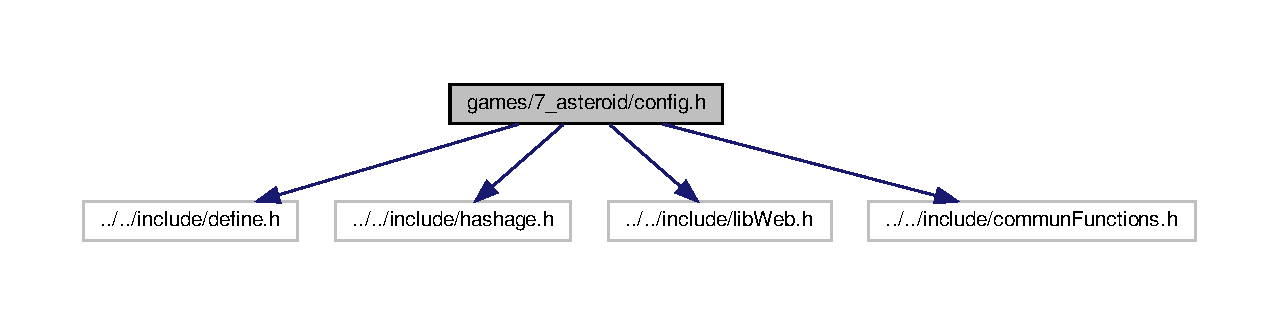
\includegraphics[width=350pt]{7__asteroid_2config_8h__incl}
\end{center}
\end{figure}
Ce graphe montre quels fichiers incluent directement ou indirectement ce fichier \+:\nopagebreak
\begin{figure}[H]
\begin{center}
\leavevmode
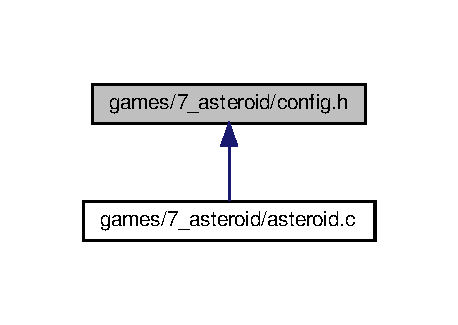
\includegraphics[width=220pt]{7__asteroid_2config_8h__dep__incl}
\end{center}
\end{figure}
\subsection*{Structures de données}
\begin{DoxyCompactItemize}
\item 
struct \hyperlink{struct_score_total}{Score\+Total}
\begin{DoxyCompactList}\small\item\em Contient des informations sur le score total. \end{DoxyCompactList}\item 
struct \hyperlink{struct_vaiss}{Vaiss}
\begin{DoxyCompactList}\small\item\em Contient des informations sur le vaisseau. \end{DoxyCompactList}\item 
struct \hyperlink{struct_asteroid}{Asteroid}
\begin{DoxyCompactList}\small\item\em Contient des informations sur un asteroide. \end{DoxyCompactList}\item 
struct \hyperlink{struct_explosion}{Explosion}
\begin{DoxyCompactList}\small\item\em Contient des informations sur l\textquotesingle{}explosion. \end{DoxyCompactList}\item 
struct \hyperlink{struct_jauge}{Jauge}
\begin{DoxyCompactList}\small\item\em Contient des informations sur la jauge. \end{DoxyCompactList}\item 
struct \hyperlink{struct_roue}{Roue}
\begin{DoxyCompactList}\small\item\em Contient des informations sur la roue. \end{DoxyCompactList}\item 
struct \hyperlink{struct_missile}{Missile}
\begin{DoxyCompactList}\small\item\em Contient des informations sur un missile. \end{DoxyCompactList}\item 
struct \hyperlink{struct_text_bonus}{Text\+Bonus}
\begin{DoxyCompactList}\small\item\em Contient des informations sur le texte à l\textquotesingle{}obtention d\textquotesingle{}un bonus. \end{DoxyCompactList}\end{DoxyCompactItemize}
\subsection*{Macros}
\begin{DoxyCompactItemize}
\item 
\#define \hyperlink{7__asteroid_2config_8h_a0ebf185842674cdecc6621333d79f8a5}{F\+R\+A\+M\+E\+\_\+\+S\+C\+O\+R\+E\+\_\+\+A\+N\+IM}~20
\item 
\#define \hyperlink{7__asteroid_2config_8h_ab5b5708a6ff360cd6e84c213661ef639}{N\+B\+\_\+\+A\+S\+T\+E\+R\+O\+I\+D\+\_\+\+F\+O\+N\+TS}~2
\item 
\#define \hyperlink{7__asteroid_2config_8h_a520fd2821a90af2ac4b3bb837bf17b12}{N\+B\+\_\+\+A\+S\+T\+E\+R\+O\+I\+D\+\_\+\+S\+O\+U\+N\+DS}~12
\item 
\#define \hyperlink{7__asteroid_2config_8h_a4fa94d9d3cf9f39200937dd319b4b87b}{T\+I\+M\+E\+\_\+\+F\+A\+D\+E\+\_\+\+IN}~400
\item 
\#define \hyperlink{7__asteroid_2config_8h_ac8b81a774ecb05419aebc49d73bd97b2}{T\+I\+M\+E\+\_\+\+F\+A\+D\+E\+\_\+\+O\+UT}~400
\item 
\#define \hyperlink{7__asteroid_2config_8h_ad2ab730880ec0195b2c9358f1af05110}{N\+B\+\_\+\+C\+H\+A\+N\+N\+E\+L\+\_\+\+E\+X\+P\+L\+O\+S\+I\+ON}~3
\item 
\#define \hyperlink{7__asteroid_2config_8h_ad7c708c0fc5593668c426b212c154e2c}{N\+B\+\_\+\+E\+X\+P\+L\+O\+S\+I\+O\+NS}~3
\item 
\#define \hyperlink{7__asteroid_2config_8h_a86e7bcd90e7564fe7f43c2b197cc6b82}{R\+A\+T\+I\+O\+\_\+\+A\+S\+T\+E\+R\+O\+I\+D\+\_\+\+E\+X\+P\+L\+O\+\_\+\+S\+I\+ZE}~1.\+2
\item 
\#define \hyperlink{7__asteroid_2config_8h_a8c7c8a93108a3a111a68ba2d01dbdaf2}{P\+R\+E\+C\+I\+S\+I\+O\+N\+\_\+\+R\+A\+N\+D\+\_\+\+F\+L\+O\+AT}~100.
\item 
\#define \hyperlink{7__asteroid_2config_8h_aa8cecfc5c5c054d2875c03e77b7be15d}{T\+R\+UE}~1
\item 
\#define \hyperlink{7__asteroid_2config_8h_a38e357a6ecaf7d313bd89e9e30dfa541}{R\+A\+Y\+O\+N\+\_\+\+V\+A\+I\+SS}~25
\item 
\#define \hyperlink{7__asteroid_2config_8h_a82d8fad64f895864e2aa8926c4ca396b}{D\+E\+C\+E\+L\+E\+R\+A\+T\+I\+ON}~1.\+015
\item 
\#define \hyperlink{7__asteroid_2config_8h_a25355a725439afc1415c598a30cf3bc9}{B\+O\+N\+U\+S\+\_\+\+D\+E\+A\+D\+\_\+\+D\+E\+C\+E\+L\+E\+R\+A\+T\+I\+ON}~0.\+05
\item 
\#define \hyperlink{7__asteroid_2config_8h_a130e8ced2d3adae7f21e9df296c2a746}{T\+U\+R\+N\+\_\+\+A\+M\+M\+O\+U\+NT}~0.\+13
\item 
\#define \hyperlink{7__asteroid_2config_8h_a01bb5f060b3487835f42c74e5267e498}{V\+I\+T\+E\+S\+SE}~10
\item 
\#define \hyperlink{7__asteroid_2config_8h_ad2d7243c099b33b2343976dd3ee8b36b}{A\+C\+C\+EL}~0.\+75
\item 
\#define \hyperlink{7__asteroid_2config_8h_a4e8a0f75f21e5116a77c9abead2a886d}{B\+A\+S\+E\+\_\+\+A\+N\+G\+LE}~3 $\ast$ \hyperlink{2__snake_2config_8h_a598a3330b3c21701223ee0ca14316eca}{PI} / 2
\item 
\#define \hyperlink{7__asteroid_2config_8h_ab793711cafbbe768ffd4fb0dbef01acf}{R\+A\+T\+I\+O\+\_\+\+A\+C\+C\+E\+L\+\_\+\+T\+U\+RN}~0.\+16
\item 
\#define \hyperlink{7__asteroid_2config_8h_a88b9efdaa83394155cda5d2c0e4fb4f1}{N\+B\+\_\+\+F\+R\+A\+M\+E\+\_\+\+T\+U\+RN}~9
\item 
\#define \hyperlink{7__asteroid_2config_8h_a0f4822a880df0adec932579f9138494e}{R\+E\+S\+E\+T\+\_\+\+T\+U\+RN}~6
\item 
\#define \hyperlink{7__asteroid_2config_8h_a1b4bc8e6cb25e856724af9cee69c7182}{N\+B\+\_\+\+F\+R\+A\+M\+E\+\_\+\+T\+H\+R\+U\+ST}~5
\item 
\#define \hyperlink{7__asteroid_2config_8h_a9543a857b985d03608052455e12dd59a}{R\+E\+S\+E\+T\+\_\+\+T\+H\+R\+U\+ST}~2
\item 
\#define \hyperlink{7__asteroid_2config_8h_af54bece7a0dbc6d81fca67a6aad1d3d3}{F\+R\+A\+M\+E\+\_\+\+I\+N\+I\+T\+\_\+\+S\+P\+A\+WN}~20
\item 
\#define \hyperlink{7__asteroid_2config_8h_aa4fe3ccc691ba865885db0c83abb4b2c}{D\+I\+S\+T\+\_\+2\+A\+S\+T\+E\+R\+O\+ID}~30
\item 
\#define \hyperlink{7__asteroid_2config_8h_a867c193becb784020b96f49c89567789}{D\+I\+S\+T\+\_\+\+V\+A\+I\+S\+S\+E\+A\+U\+\_\+\+A\+S\+T\+E\+R\+O\+ID}~300
\item 
\#define \hyperlink{7__asteroid_2config_8h_a367d02be23938557734167f64c02eaa0}{F\+R\+A\+M\+E\+\_\+\+A\+P\+P\+A\+R\+I\+T\+I\+O\+N\+\_\+\+A\+S\+T\+E\+R\+O\+ID}~(16$\ast$ \hyperlink{7__asteroid_2config_8h_a85f9d29551f1bf30f03229da27cb532f}{F\+R\+A\+M\+E\+S\+\_\+\+P\+E\+R\+\_\+\+S\+E\+C\+O\+ND})
\item 
\#define \hyperlink{7__asteroid_2config_8h_a74dce507516728630bc30ef7b972c1c0}{V\+I\+T\+E\+S\+S\+E\+\_\+\+S\+P\+A\+W\+N\+\_\+\+I\+N\+IT}~(\hyperlink{7__asteroid_2config_8h_a85f9d29551f1bf30f03229da27cb532f}{F\+R\+A\+M\+E\+S\+\_\+\+P\+E\+R\+\_\+\+S\+E\+C\+O\+ND}$\ast$12)
\item 
\#define \hyperlink{7__asteroid_2config_8h_a1a4378a760568e6d429f03d9a7c789c6}{V\+I\+T\+E\+S\+S\+E\+\_\+\+S\+P\+A\+W\+N\+\_\+\+M\+IN}~(\hyperlink{7__asteroid_2config_8h_a85f9d29551f1bf30f03229da27cb532f}{F\+R\+A\+M\+E\+S\+\_\+\+P\+E\+R\+\_\+\+S\+E\+C\+O\+ND}$\ast$6.\+5)
\item 
\#define \hyperlink{7__asteroid_2config_8h_a49ef28c6ca8e5b17abc7a959460e0fe3}{A\+C\+C\+E\+L\+E\+R\+A\+T\+I\+O\+N\+\_\+\+S\+P\+A\+WN}~0.\+03
\item 
\#define \hyperlink{7__asteroid_2config_8h_ab6825030e5a2ad03f808fdc9b906fac0}{F\+R\+A\+M\+E\+\_\+2\+A\+S\+T\+E\+R\+O\+ID}~(\hyperlink{7__asteroid_2config_8h_a85f9d29551f1bf30f03229da27cb532f}{F\+R\+A\+M\+E\+S\+\_\+\+P\+E\+R\+\_\+\+S\+E\+C\+O\+ND}/2)
\item 
\#define \hyperlink{7__asteroid_2config_8h_aadb09f40a02b5e53176d185bfa68525f}{P\+V\+\_\+\+B\+A\+SE}~1.\+2
\item 
\#define \hyperlink{7__asteroid_2config_8h_a27850c6d9e07217ed9ba3fac6eddc274}{V\+I\+T\+E\+S\+S\+E\+\_\+\+B\+A\+SE}~3
\item 
\#define \hyperlink{7__asteroid_2config_8h_a083062c9ab1a34bb4973fa42ef8d1fb1}{M\+A\+X\+\_\+\+A\+S\+T\+E\+R\+O\+I\+D\+\_\+\+S\+I\+ZE}~90
\item 
\#define \hyperlink{7__asteroid_2config_8h_af02879b9632680b60be79e865b7fe3e6}{T\+A\+I\+L\+L\+E\+\_\+\+M\+I\+N\+\_\+\+S\+P\+L\+IT}~36
\item 
\#define \hyperlink{7__asteroid_2config_8h_a0324b414e456891368832c5b9e41e832}{T\+A\+I\+L\+L\+E\+\_\+\+M\+I\+N\+\_\+\+A\+S\+T\+E\+R\+O\+ID}~18
\item 
\#define \hyperlink{7__asteroid_2config_8h_ae5d3fd03efff7ea8fa5f4f107f6a17a8}{V\+I\+T\+E\+S\+S\+E\+\_\+\+M\+A\+X\+\_\+\+A\+S\+T\+E\+R\+O\+ID}~22
\item 
\#define \hyperlink{7__asteroid_2config_8h_a538099a79a3562dfb035e19bc15d68de}{V\+I\+T\+E\+S\+S\+E\+\_\+\+M\+A\+X\+\_\+\+A\+S\+T\+E\+R\+O\+I\+D\+\_\+\+H\+A\+R\+D\+C\+O\+RE}~30
\item 
\#define \hyperlink{7__asteroid_2config_8h_aa390e01494054ae0fe9a4f55624915bd}{V\+I\+T\+E\+S\+S\+E\+\_\+\+M\+I\+N\+\_\+\+A\+S\+T\+E\+R\+O\+ID}~9
\item 
\#define \hyperlink{7__asteroid_2config_8h_aec0384f1b98985dff50f645e84bdf0f2}{S\+T\+A\+R\+T\+\_\+\+D\+I\+F\+F\+I\+C\+U\+L\+TE}~1.\+01
\item 
\#define \hyperlink{7__asteroid_2config_8h_a60b40f56c11dab83d832d4ad4bee30b5}{D\+I\+F\+F\+I\+C\+U\+L\+T\+E\+\_\+\+M\+I\+N\+\_\+\+S\+P\+L\+IT}~5
\item 
\#define \hyperlink{7__asteroid_2config_8h_a72d24b98214f3c2e864689b358ede3b3}{R\+A\+T\+I\+O\+\_\+\+D\+I\+F\+F\+I\+C\+U\+L\+T\+E\+\_\+\+A\+U\+G\+M\+E\+NT}~0.\+0027
\item 
\#define \hyperlink{7__asteroid_2config_8h_af5694824a1f3b87d24cefdc9a73884b9}{R\+A\+T\+I\+O\+\_\+\+D\+I\+F\+F\+I\+C\+U\+L\+T\+E\+\_\+\+A\+U\+G\+M\+E\+N\+T\+\_\+\+M\+U\+L\+TI}~0.\+00033
\item 
\#define \hyperlink{7__asteroid_2config_8h_a2c9abf82f8cc72408c5a7b76daedd54d}{M\+A\+X\+\_\+\+V\+I\+T\+E\+S\+S\+E\+\_\+\+R\+O\+TA}~15
\item 
\#define \hyperlink{7__asteroid_2config_8h_a8e5034a0493e51b9c7db570e3510feea}{N\+B\+\_\+\+A\+S\+T\+E\+\_\+\+T\+E\+X\+T\+U\+R\+ES}~6
\item 
\#define \hyperlink{7__asteroid_2config_8h_aa26f2abfb75d6954c0dd07183121c23f}{N\+B\+\_\+\+T\+R\+A\+N\+C\+H\+E\+\_\+\+T\+A\+I\+L\+LE}~4
\item 
\#define \hyperlink{7__asteroid_2config_8h_a5461d80ad074bdfa729ab899767d7739}{N\+B\+\_\+\+T\+A\+I\+L\+L\+E\+\_\+\+A\+S\+TE}~2
\item 
\#define \hyperlink{7__asteroid_2config_8h_aa422d6fe9012d53a7e7d4380d41b090b}{N\+B\+\_\+\+F\+I\+S\+S\+U\+R\+ES}~2
\item 
\#define \hyperlink{7__asteroid_2config_8h_a1605a24e037309a2d85ed0e8dfcb6926}{M\+A\+X\+\_\+\+D\+I\+FF}~40
\item 
\#define \hyperlink{7__asteroid_2config_8h_a3191acbabe1143c2edbaf5d8244647da}{I\+N\+T\+E\+R\+V\+A\+L\+E\+\_\+\+R\+A\+N\+D\+\_\+\+D\+I\+F\+F\+I\+C\+U\+L\+TE}~0.\+3
\item 
\#define \hyperlink{7__asteroid_2config_8h_a3ab9d4d138157a3616c54d162dc3c6b4}{F\+R\+A\+M\+E\+\_\+\+H\+I\+T\+\_\+\+A\+N\+IM}~2
\item 
\#define \hyperlink{7__asteroid_2config_8h_a66c186ad8fdc49e41743279ab4b7cb3b}{F\+R\+A\+M\+E\+\_\+\+V\+A\+G\+U\+E\+\_\+\+I\+N\+IT}~(4.\+28$\ast$\hyperlink{7__asteroid_2config_8h_a85f9d29551f1bf30f03229da27cb532f}{F\+R\+A\+M\+E\+S\+\_\+\+P\+E\+R\+\_\+\+S\+E\+C\+O\+ND})
\item 
\#define \hyperlink{7__asteroid_2config_8h_ae17dfb36ca43503a93859b915348c610}{F\+R\+A\+M\+E\+\_\+\+D\+E\+P\+A\+RT}~24
\item 
\#define \hyperlink{7__asteroid_2config_8h_afb63fb9f349f47a97b92f3cad23e3e60}{D\+I\+S\+T\+\_\+\+S\+P\+A\+W\+N\+\_\+2\+A\+S\+T\+E\+R\+O\+ID}~40
\item 
\#define \hyperlink{7__asteroid_2config_8h_a4b7da9eaf833652dbeebc0ec44de936d}{S\+P\+E\+E\+D\+\_\+\+H\+A\+R\+D\+C\+O\+RE}~2.\+1
\item 
\#define \hyperlink{7__asteroid_2config_8h_a9b87682f53ffda9c807c82a1e2a68692}{N\+B\+\_\+\+R\+O\+U\+E\+\_\+\+E\+M\+P\+L\+A\+C\+E\+M\+E\+N\+TS}~5
\item 
\#define \hyperlink{7__asteroid_2config_8h_a86127395915e59ff5ccf9f126da48ac8}{N\+B\+\_\+\+A\+R\+R\+O\+U\+N\+D\+\_\+\+J\+A\+U\+G\+ES}~4
\item 
\#define \hyperlink{7__asteroid_2config_8h_aa6f50319f3c88e48eee673f118098849}{M\+I\+N\+\_\+\+R\+A\+T\+I\+O\+\_\+\+C\+O\+L\+OR}~0.\+3
\item 
\#define \hyperlink{7__asteroid_2config_8h_ade0b1b60a8d3061799f26048ca432100}{R\+A\+T\+I\+O\+\_\+\+C\+O\+L\+O\+R\+\_\+\+J\+A\+U\+GE}~0.\+72
\item 
\#define \hyperlink{7__asteroid_2config_8h_aec076af9a7f22f9e7b75d89af7b69cf9}{F\+R\+A\+M\+E\+\_\+\+R\+O\+T\+A\+\_\+\+R\+O\+UE}~13
\item 
\#define \hyperlink{7__asteroid_2config_8h_a2abb3de4b868eb0585d073d57186ab80}{F\+R\+A\+M\+E\+\_\+\+A\+M\+MO}~7
\item 
\#define \hyperlink{7__asteroid_2config_8h_ad3e3c131127104b015d71bb7da542039}{B\+L\+O\+C\+K\+I\+N\+G\+\_\+\+A\+N\+IM}~1
\item 
\#define \hyperlink{7__asteroid_2config_8h_ada4bca62a7b42b394ec20349e16e209d}{N\+B\+\_\+\+M\+I\+S\+S\+I\+L\+ES}~5
\item 
\#define \hyperlink{7__asteroid_2config_8h_a042aff171ca8fc67ec290883be13e7f1}{B\+A\+S\+E\+\_\+\+Z\+I\+G\+Z\+A\+G\+\_\+\+A\+N\+G\+LE}~0.\+1
\item 
\#define \hyperlink{7__asteroid_2config_8h_a1558c6eb803a19bd6e24b87941f9c59c}{I\+N\+T\+E\+R\+V\+A\+L\+L\+E\+\_\+\+Z\+I\+G\+Z\+A\+G\+\_\+\+A\+N\+G\+LE}~0.\+05
\item 
\#define \hyperlink{7__asteroid_2config_8h_a73196e7f8821c43bbe9c5658ecb2d83c}{F\+R\+A\+M\+E\+\_\+\+T\+O\+\_\+\+R\+E\+A\+C\+H\+\_\+\+A\+N\+G\+LE}~4
\item 
\#define \hyperlink{7__asteroid_2config_8h_a4305f182e04ef5162040e4f6c0ba9e5b}{A\+N\+G\+L\+E\+\_\+\+T\+E\+L\+E\+G\+U\+I\+DE}~0.\+1
\item 
\#define \hyperlink{7__asteroid_2config_8h_a4a8aa7578e2e94c8ed0ac1a84c6fcdb0}{C\+H\+A\+M\+P\+\_\+\+V\+I\+S\+I\+O\+N\+\_\+\+T\+E\+L\+E\+G\+U\+I\+DE}~(\hyperlink{2__snake_2config_8h_a598a3330b3c21701223ee0ca14316eca}{PI}/2)
\item 
\#define \hyperlink{7__asteroid_2config_8h_acc4840ef85870c593a211f6abde0e463}{N\+B\+\_\+\+L\+A\+S\+E\+R\+\_\+\+B\+E\+AM}~8
\item 
\#define \hyperlink{7__asteroid_2config_8h_a236d0ccf33f6056f911f5148d6145d39}{L\+A\+S\+E\+R\+\_\+\+A\+C\+C\+EL}~0.\+05
\item 
\#define \hyperlink{7__asteroid_2config_8h_af84625e32b007c66dad7b405c0885f5d}{B\+A\+S\+E\+\_\+\+T\+A\+I\+L\+L\+E\+\_\+\+E\+X\+P\+L\+O\+S\+I\+ON}~40
\item 
\#define \hyperlink{7__asteroid_2config_8h_a5202c9342f09b8f704493e6f460dbe40}{R\+A\+T\+I\+O\+\_\+\+D\+M\+G\+\_\+\+U\+P\+\_\+\+L\+A\+S\+ER}~0.\+9
\item 
\#define \hyperlink{7__asteroid_2config_8h_a880a9368f0ff5ad7191636759070180e}{D\+E\+A\+D\+\_\+\+F\+R\+O\+Z\+EN}~-\/999
\item 
\#define \hyperlink{7__asteroid_2config_8h_a0c7c8ce4f51e9231d7c5815e09758bb5}{D\+I\+S\+T\+A\+N\+C\+E\+\_\+\+C\+A\+N\+ON}~23
\item 
\#define \hyperlink{7__asteroid_2config_8h_a4563e322ab3b48c9fe9d84c755db6cf8}{F\+R\+E\+Q\+U\+E\+N\+C\+E\+\_\+\+B\+A\+SE}~(\hyperlink{7__asteroid_2config_8h_a85f9d29551f1bf30f03229da27cb532f}{F\+R\+A\+M\+E\+S\+\_\+\+P\+E\+R\+\_\+\+S\+E\+C\+O\+ND}/2)
\item 
\#define \hyperlink{7__asteroid_2config_8h_a1fb05fa9aac1e8e1b3cdd9cf32a4cfc1}{B\+A\+S\+E\+\_\+\+V\+I\+T\+E\+S\+S\+E\+\_\+\+M\+I\+S\+S\+I\+LE}~15
\item 
\#define \hyperlink{7__asteroid_2config_8h_a153cf1d5572254c3b75196055e5b660e}{B\+A\+S\+E\+\_\+\+D\+E\+G\+A\+T\+\_\+\+M\+I\+S\+S\+I\+LE}~1.\+5
\item 
\#define \hyperlink{7__asteroid_2config_8h_a229c39288605ee702940dec249381452}{D\+U\+R\+E\+E\+\_\+\+M\+I\+S\+S\+I\+L\+E\+\_\+\+B\+A\+SE}~(2$\ast$\hyperlink{7__asteroid_2config_8h_a85f9d29551f1bf30f03229da27cb532f}{F\+R\+A\+M\+E\+S\+\_\+\+P\+E\+R\+\_\+\+S\+E\+C\+O\+ND})
\item 
\#define \hyperlink{7__asteroid_2config_8h_aa1ac23c9deb598d55a6c57c25e67187e}{M\+A\+X\+\_\+\+R\+A\+T\+I\+O\+\_\+\+A\+M\+M\+O\+\_\+\+O\+B\+T\+A\+I\+N\+A\+B\+LE}~(0.\+7)
\item 
\#define \hyperlink{7__asteroid_2config_8h_a6f739e7becfffb0dae9365d1bce80ef2}{A\+M\+M\+O\+\_\+\+G\+R\+A\+NT}~(1./3)
\item 
\#define \hyperlink{7__asteroid_2config_8h_a1f286ccdb17e67adc116628ca8048577}{M\+I\+S\+S\+I\+L\+E\+\_\+\+C\+UT}~56
\item 
\#define \hyperlink{7__asteroid_2config_8h_aed81eb575ba3469d1154bc05e5655772}{F\+R\+A\+M\+E\+\_\+\+M\+I\+S\+S\+I\+L\+E\+\_\+\+D\+E\+A\+TH}~8
\item 
\#define \hyperlink{7__asteroid_2config_8h_a85f9d29551f1bf30f03229da27cb532f}{F\+R\+A\+M\+E\+S\+\_\+\+P\+E\+R\+\_\+\+S\+E\+C\+O\+ND}~30
\item 
\#define \hyperlink{7__asteroid_2config_8h_a5b6610f9d69984ecba58bcd37b3c1be1}{F\+R\+A\+M\+E\+\_\+\+S\+H\+O\+W\+\_\+\+H\+E\+LP}~-\/50
\item 
\#define \hyperlink{7__asteroid_2config_8h_a49cb9e7f6e11529527802f1188a44921}{F\+R\+A\+M\+E\+\_\+\+D\+E\+S\+T\+R\+O\+Y\+\_\+\+A\+S\+TE}~-\/30
\item 
\#define \hyperlink{7__asteroid_2config_8h_a0ccacc3ecbbc935176fd11454ecb79d6}{N\+B\+\_\+\+B\+O\+N\+US}~9
\item 
\#define \hyperlink{7__asteroid_2config_8h_ae1cfd4c65bedcc92ee36aaab568fb83d}{N\+O\+\_\+\+B\+O\+N\+US}~-\/1
\item 
\#define \hyperlink{7__asteroid_2config_8h_a8271f0bb542462f1c9f2304605c0434f}{P\+R\+O\+B\+A\+\_\+\+B\+O\+N\+US}~3
\item 
\#define \hyperlink{7__asteroid_2config_8h_a92f2c26a8843f0541c86537af936437d}{N\+B\+\_\+\+T\+I\+R\+\_\+\+M\+AX}~3
\item 
\#define \hyperlink{7__asteroid_2config_8h_ad8292ff6d99fb255c69b1748f39b3ad5}{N\+B\+\_\+\+B\+O\+N\+U\+S\+\_\+\+P\+O\+I\+NT}~3
\item 
\#define \hyperlink{7__asteroid_2config_8h_ae0c22d64ea65c9b96120e7937a9d385d}{M\+A\+X\+\_\+\+B\+O\+M\+B\+E\+\_\+\+N\+U\+C\+L\+E\+A\+I\+RE}~1
\item 
\#define \hyperlink{7__asteroid_2config_8h_ad1ceaf0f3d078698c1f9cb967b6b2bcc}{M\+A\+X\+\_\+\+T\+E\+X\+T\+\_\+\+B\+O\+N\+US}~10
\item 
\#define \hyperlink{7__asteroid_2config_8h_a20c6057a89989a489e7a2aaae04c68f5}{F\+R\+A\+M\+E\+\_\+\+S\+H\+O\+W\+\_\+\+B\+O\+N\+U\+S\+\_\+\+T\+E\+XT}~30
\item 
\#define \hyperlink{7__asteroid_2config_8h_a3a0fd00eeac2ad701e77975739bd35f6}{E\+S\+P\+A\+C\+E\+M\+E\+N\+T\+\_\+\+S\+H\+O\+W\+\_\+\+T\+E\+XT}~70
\item 
\#define \hyperlink{7__asteroid_2config_8h_a8e869e2f265747e788850e24792f6773}{S\+I\+Z\+E\+\_\+\+B\+O\+N\+U\+S\+\_\+\+T\+E\+XT}~44.
\item 
\#define \hyperlink{7__asteroid_2config_8h_a132c4d592b86925dca028243542435c6}{B\+O\+N\+U\+S\+\_\+\+A\+C\+C\+E\+L\+E\+R\+A\+T\+I\+O\+N\+\_\+\+M\+I\+S\+S\+I\+LE}~1.\+7
\item 
\#define \hyperlink{7__asteroid_2config_8h_acc2301597c373ea5c2e44c28afacd096}{V\+I\+T\+E\+S\+S\+E\+\_\+\+M\+I\+S\+S\+I\+L\+E\+\_\+\+M\+AX}~(2$\ast$\hyperlink{7__asteroid_2config_8h_a1fb05fa9aac1e8e1b3cdd9cf32a4cfc1}{B\+A\+S\+E\+\_\+\+V\+I\+T\+E\+S\+S\+E\+\_\+\+M\+I\+S\+S\+I\+LE})
\item 
\#define \hyperlink{7__asteroid_2config_8h_a7e64d280ad41a6e8860907d35dceee12}{B\+O\+N\+U\+S\+\_\+\+F\+R\+E\+Q\+U\+E\+N\+C\+E\+\_\+\+M\+I\+S\+S\+I\+LE}~1.\+4
\item 
\#define \hyperlink{7__asteroid_2config_8h_a0dc68d121caff8ce538a983b66bf32ed}{F\+R\+E\+Q\+U\+E\+N\+C\+E\+\_\+\+M\+I\+S\+S\+I\+L\+E\+\_\+\+M\+IN}~(\hyperlink{7__asteroid_2config_8h_a85f9d29551f1bf30f03229da27cb532f}{F\+R\+A\+M\+E\+S\+\_\+\+P\+E\+R\+\_\+\+S\+E\+C\+O\+ND}/6.)
\item 
\#define \hyperlink{7__asteroid_2config_8h_a65e2bceb8fa36eeaa96da771b679c2be}{D\+E\+G\+A\+T\+\_\+\+M\+I\+S\+S\+I\+L\+E\+\_\+\+M\+AX}~6
\item 
\#define \hyperlink{7__asteroid_2config_8h_a532725482c7898789a71e019f613ed85}{D\+E\+G\+A\+T\+\_\+\+A\+DD}~0.\+75
\item 
\#define \hyperlink{7__asteroid_2config_8h_af4e038d21c306161bb8c70cdf4a28985}{F\+R\+A\+M\+E\+\_\+\+B\+O\+M\+B\+E\+\_\+\+N\+U\+C\+L\+E\+A\+I\+RE}~(\hyperlink{7__asteroid_2config_8h_a85f9d29551f1bf30f03229da27cb532f}{F\+R\+A\+M\+E\+S\+\_\+\+P\+E\+R\+\_\+\+S\+E\+C\+O\+ND}$\ast$1.\+5)
\item 
\#define \hyperlink{7__asteroid_2config_8h_aaae5de8a7b1eb20d7e9c69ffbc2384e2}{F\+R\+A\+M\+E\+\_\+\+A\+N\+I\+M\+\_\+\+B\+O\+MB}~24
\item 
\#define \hyperlink{7__asteroid_2config_8h_a9e5b4adfefe9009bc09eaf78738c0db8}{N\+B\+\_\+\+A\+N\+I\+M\+\_\+\+B\+O\+MB}~16
\item 
\#define \hyperlink{7__asteroid_2config_8h_a20e65cb991369765500db37b9089cdb8}{F\+R\+A\+M\+E\+\_\+\+K\+I\+L\+L\+\_\+\+A\+S\+T\+E\+R\+O\+\_\+\+B\+O\+MB}~15
\item 
\#define \hyperlink{7__asteroid_2config_8h_adeea677a5f008ccf5f43a0da5b2793f1}{N\+B\+\_\+\+R\+O\+W\+\_\+\+B\+O\+MB}~4
\item 
\#define \hyperlink{7__asteroid_2config_8h_a73ac4b641b9f81be39d541e4eb48b82c}{N\+B\+\_\+\+C\+O\+L\+\_\+\+B\+O\+MB}~4
\end{DoxyCompactItemize}
\subsection*{Énumérations}
\begin{DoxyCompactItemize}
\item 
enum \hyperlink{7__asteroid_2config_8h_ad92d52a794b5305986ad03061e2c25cf}{F\+O\+N\+TS} \{ \hyperlink{7__asteroid_2config_8h_ad92d52a794b5305986ad03061e2c25cfa28a3b29845b04d5a4787681206f8a03d}{F\+O\+N\+T\+\_\+\+B\+O\+N\+US}, 
\hyperlink{7__asteroid_2config_8h_ad92d52a794b5305986ad03061e2c25cfad2961fbcba9784d7f35f2a6e7799759d}{F\+O\+N\+T\+\_\+\+S\+C\+O\+RE}
 \}
\item 
enum \hyperlink{7__asteroid_2config_8h_a084b0c48898b48ae7e1379c594e0ed30}{S\+O\+U\+N\+DS} \{ \newline
\hyperlink{7__asteroid_2config_8h_a084b0c48898b48ae7e1379c594e0ed30a86cd12e192f09cd44ce2f9d4fa2df159}{S\+O\+U\+N\+D\+\_\+\+S\+H\+O\+OT}, 
\hyperlink{7__asteroid_2config_8h_a084b0c48898b48ae7e1379c594e0ed30ab10cc58e9bce4306cf9e29e6227f9d2b}{S\+O\+U\+N\+D\+\_\+\+S\+H\+O\+O\+T\+\_\+\+Z\+I\+G\+Z\+AG}, 
\hyperlink{7__asteroid_2config_8h_a084b0c48898b48ae7e1379c594e0ed30ad4ef88640a5284d68d56ad7e3b0cda18}{S\+O\+U\+N\+D\+\_\+\+S\+H\+O\+O\+T\+\_\+\+T\+E\+L\+E\+G\+U\+I\+DE}, 
\hyperlink{7__asteroid_2config_8h_a084b0c48898b48ae7e1379c594e0ed30ae9ae95d1d12fbfba3b7ec8526c61166a}{S\+O\+U\+N\+D\+\_\+\+S\+H\+O\+O\+T\+\_\+\+G\+L\+A\+CE}, 
\newline
\hyperlink{7__asteroid_2config_8h_a084b0c48898b48ae7e1379c594e0ed30a1501464ef97bf2e5dba4a5365fe5154c}{S\+O\+U\+N\+D\+\_\+\+L\+A\+S\+E\+R\+\_\+\+B\+E\+AM}, 
\hyperlink{7__asteroid_2config_8h_a084b0c48898b48ae7e1379c594e0ed30a8dc509f9c01b07b3373ca0be1e0bbc9e}{S\+O\+U\+N\+D\+\_\+\+B\+O\+N\+US}, 
\hyperlink{7__asteroid_2config_8h_a084b0c48898b48ae7e1379c594e0ed30a70b644f29fff15e2bb258fb9f4c8c9d0}{S\+O\+U\+N\+D\+\_\+\+H\+IT}, 
\hyperlink{7__asteroid_2config_8h_a084b0c48898b48ae7e1379c594e0ed30ada6fd4263cd43f4f5d5c4e29b86d5352}{S\+O\+U\+N\+D\+\_\+\+I\+C\+E\+\_\+\+E\+X\+P\+LO}, 
\newline
\hyperlink{7__asteroid_2config_8h_a084b0c48898b48ae7e1379c594e0ed30a5a0f7d9bf53bb2e4519e16992005bf1a}{S\+O\+U\+N\+D\+\_\+\+E\+X\+P\+LO}, 
\hyperlink{7__asteroid_2config_8h_a084b0c48898b48ae7e1379c594e0ed30ae81e9f820fa7bc4777aa9f46019f29bd}{B\+I\+G\+\_\+\+E\+X\+P\+LO}, 
\hyperlink{7__asteroid_2config_8h_a084b0c48898b48ae7e1379c594e0ed30ad20b05ef589944c25dd727bdd0badeb0}{S\+O\+U\+N\+D\+\_\+\+T\+H\+R\+U\+ST}, 
\hyperlink{7__asteroid_2config_8h_a084b0c48898b48ae7e1379c594e0ed30a3c84a26eed13f1442e465fd3b2e64434}{S\+O\+U\+N\+D\+\_\+\+G\+A\+M\+E\+O\+V\+ER}
 \}
\item 
enum \{ \hyperlink{7__asteroid_2config_8h_a0411cd49bb5b71852cecd93bcbf0ca2da1efa724a722d3e42a1eeca162d3e35e1}{T\+H\+R\+U\+S\+T\+\_\+\+UP}, 
\hyperlink{7__asteroid_2config_8h_a0411cd49bb5b71852cecd93bcbf0ca2daa3b97e6087fb50166fdc894dabf23923}{T\+H\+R\+U\+S\+T\+\_\+\+L\+E\+FT}, 
\hyperlink{7__asteroid_2config_8h_a0411cd49bb5b71852cecd93bcbf0ca2da322165874c218fd1bf46661dffee3a50}{T\+H\+R\+U\+S\+T\+\_\+\+R\+I\+G\+HT}
 \}
\item 
enum \hyperlink{7__asteroid_2config_8h_af974e57579aa5197c4982de9eb7607b9}{E\+X\+P\+L\+O\+S\+I\+O\+NS} \{ \hyperlink{7__asteroid_2config_8h_af974e57579aa5197c4982de9eb7607b9a76ff75d159f3f858e95e68696dab357a}{E\+X\+P\+L\+O\+\_\+\+M\+I\+S\+S\+I\+LE}, 
\hyperlink{7__asteroid_2config_8h_af974e57579aa5197c4982de9eb7607b9ac166d2f44348c5a805d574361fe6d13d}{E\+X\+P\+L\+O\+\_\+\+A\+S\+TE}, 
\hyperlink{7__asteroid_2config_8h_af974e57579aa5197c4982de9eb7607b9a5820b3bd1d86ce2f1463a1e6bded5c2e}{E\+X\+P\+L\+O\+\_\+\+G\+L\+A\+CE}
 \}
\item 
enum \hyperlink{7__asteroid_2config_8h_a610033eba3b8e7fcb6d5284a70ab5e26}{dir\+\_\+turn} \{ \hyperlink{7__asteroid_2config_8h_a610033eba3b8e7fcb6d5284a70ab5e26a3f8787368a9aa87f0bde02c09574a1df}{N\+O\+\_\+\+T\+U\+RN}, 
\hyperlink{7__asteroid_2config_8h_a610033eba3b8e7fcb6d5284a70ab5e26adb45120aafd37a973140edee24708065}{L\+E\+FT}, 
\hyperlink{7__asteroid_2config_8h_a610033eba3b8e7fcb6d5284a70ab5e26aec8379af7490bb9eaaf579cf17876f38}{R\+I\+G\+HT}, 
\hyperlink{7__asteroid_2config_8h_a610033eba3b8e7fcb6d5284a70ab5e26a627abe5a430420baf29ebe1940a7f2fb}{B\+O\+TH}
 \}
\item 
enum \hyperlink{7__asteroid_2config_8h_ad2ef04bd701ad364078ae0bd1afd6012}{shots} \{ \newline
\hyperlink{7__asteroid_2config_8h_ad2ef04bd701ad364078ae0bd1afd6012aa74b8aa45938cb6274229dda4244bfdf}{S\+H\+O\+T\+\_\+\+N\+O\+R\+M\+AL}, 
\hyperlink{7__asteroid_2config_8h_ad2ef04bd701ad364078ae0bd1afd6012ac5819da9ee63928afdf901dae24510fe}{S\+H\+O\+T\+\_\+\+Z\+I\+G\+Z\+AG}, 
\hyperlink{7__asteroid_2config_8h_ad2ef04bd701ad364078ae0bd1afd6012a5db38b985b3549e1030a4f48a1aa1d16}{S\+H\+O\+T\+\_\+\+T\+E\+L\+E\+G\+U\+I\+DE}, 
\hyperlink{7__asteroid_2config_8h_ad2ef04bd701ad364078ae0bd1afd6012ab972c96a50c110bb807e749a89833e6c}{S\+H\+O\+T\+\_\+\+G\+L\+A\+CE}, 
\newline
\hyperlink{7__asteroid_2config_8h_ad2ef04bd701ad364078ae0bd1afd6012a771820a6dcb12d44c8d149235d6d1320}{S\+H\+O\+T\+\_\+\+L\+A\+S\+ER}
 \}
\item 
enum \hyperlink{7__asteroid_2config_8h_a5c055da78bfd0ead31125cf3f3c6fbb6}{taille\+\_\+bonus} \{ \hyperlink{7__asteroid_2config_8h_a5c055da78bfd0ead31125cf3f3c6fbb6aee66d881e873b981297334e790f60c1a}{P\+E\+T\+IT}, 
\hyperlink{7__asteroid_2config_8h_a5c055da78bfd0ead31125cf3f3c6fbb6aee96574eabbfbe329a44b059e4652351}{M\+O\+Y\+EN}, 
\hyperlink{7__asteroid_2config_8h_a5c055da78bfd0ead31125cf3f3c6fbb6a30625632affab2bcd18da495e1105ecb}{G\+R\+A\+ND}
 \}
\item 
enum \hyperlink{7__asteroid_2config_8h_a229077b6da581cb56adde9d613e02573}{bonus\+\_\+e} \{ \newline
\hyperlink{7__asteroid_2config_8h_a229077b6da581cb56adde9d613e02573a271c87e4b359d9671a7e1c5702a0f794}{T\+I\+R\+\_\+\+M\+U\+L\+T\+I\+P\+LE}, 
\hyperlink{7__asteroid_2config_8h_a229077b6da581cb56adde9d613e02573a3436d76a8c9425b7433a05c80ece0e54}{B\+O\+U\+C\+L\+I\+ER}, 
\hyperlink{7__asteroid_2config_8h_a229077b6da581cb56adde9d613e02573af9e6e93d2a3ef928c1c60676f09fce8b}{V\+I\+T\+E\+S\+S\+E\+\_\+\+D\+E\+\_\+\+T\+IR}, 
\hyperlink{7__asteroid_2config_8h_a229077b6da581cb56adde9d613e02573acf38ba132630b9624727dac63e7f72a5}{B\+O\+N\+U\+S\+\_\+\+V\+I\+T\+E\+S\+S\+E\+\_\+\+M\+I\+S\+S\+I\+LE}, 
\newline
\hyperlink{7__asteroid_2config_8h_a229077b6da581cb56adde9d613e02573a03e725c8dd07724161e6279c6f25ec23}{D\+E\+G\+AT}, 
\hyperlink{7__asteroid_2config_8h_a229077b6da581cb56adde9d613e02573acc0b2a29ba239dab6a8eac7e5a343e7b}{B\+O\+M\+B\+E\+\_\+\+N\+U\+C\+L\+E\+A\+I\+RE}, 
\hyperlink{7__asteroid_2config_8h_a229077b6da581cb56adde9d613e02573a01a455b23120bd4cf2d679477f04bc0a}{P\+O\+I\+N\+T\+\_\+\+P\+E\+T\+IT}, 
\hyperlink{7__asteroid_2config_8h_a229077b6da581cb56adde9d613e02573a5f4c7a11779341968d176e199bdf0439}{P\+O\+I\+N\+T\+\_\+\+M\+O\+Y\+EN}, 
\newline
\hyperlink{7__asteroid_2config_8h_a229077b6da581cb56adde9d613e02573a1af9aa71bd375dd18a71e16b8ab97ab2}{P\+O\+I\+N\+T\+\_\+\+G\+R\+A\+ND}
 \}
\end{DoxyCompactItemize}
\subsection*{Variables}
\begin{DoxyCompactItemize}
\item 
const S\+D\+L\+\_\+\+Color \hyperlink{7__asteroid_2config_8h_a776a7ff0aa9e3316de82682b96592bf8}{S\+C\+O\+R\+E\+\_\+\+C\+O\+L\+OR} = \{0x44,0xdd,0x\+F\+F\}
\item 
static const S\+D\+L\+\_\+\+Color \hyperlink{7__asteroid_2config_8h_a4223eebf2e076b331940f83bc3285bee}{H\+U\+D\+\_\+\+C\+O\+L\+OR} = \{0x2f,0x30,0x4f\}
\item 
char $\ast$ \hyperlink{7__asteroid_2config_8h_ae901b87296360a66db1ee112f1a5c44a}{D\+I\+R\+\_\+\+F\+O\+N\+T\+S\+\_\+\+A\+S\+T\+E\+R\+O\+ID} \mbox{[}\hyperlink{7__asteroid_2config_8h_ab5b5708a6ff360cd6e84c213661ef639}{N\+B\+\_\+\+A\+S\+T\+E\+R\+O\+I\+D\+\_\+\+F\+O\+N\+TS}\mbox{]}
\item 
char $\ast$ \hyperlink{7__asteroid_2config_8h_a992307868c261a777620ec2d62c97360}{D\+I\+R\+\_\+\+S\+O\+U\+N\+D\+S\+\_\+\+A\+S\+T\+E\+R\+O\+ID} \mbox{[}\hyperlink{7__asteroid_2config_8h_a520fd2821a90af2ac4b3bb837bf17b12}{N\+B\+\_\+\+A\+S\+T\+E\+R\+O\+I\+D\+\_\+\+S\+O\+U\+N\+DS}\mbox{]}
\item 
static int \hyperlink{7__asteroid_2config_8h_a2d7328a301fb2bf2583daf7c188f5649}{S\+O\+U\+N\+D\+\_\+\+V\+O\+L\+U\+M\+ES} \mbox{[}\hyperlink{7__asteroid_2config_8h_a520fd2821a90af2ac4b3bb837bf17b12}{N\+B\+\_\+\+A\+S\+T\+E\+R\+O\+I\+D\+\_\+\+S\+O\+U\+N\+DS}\mbox{]} = \{30,110,17,85,25, 128, 12,50, 115,128, 100, 100\}
\item 
const int \hyperlink{7__asteroid_2config_8h_a59768e15ccd384331f91425238e9b9b5}{F\+R\+A\+M\+E\+\_\+\+E\+X\+P\+L\+O\+S\+I\+O\+NS} \mbox{[}\hyperlink{7__asteroid_2config_8h_ad7c708c0fc5593668c426b212c154e2c}{N\+B\+\_\+\+E\+X\+P\+L\+O\+S\+I\+O\+NS}\mbox{]} = \{12, 20, 20\}
\item 
const int \hyperlink{7__asteroid_2config_8h_ae12bcc2a9eec7e7b021f58156ada176e}{N\+B\+\_\+\+A\+N\+I\+M\+\_\+\+E\+X\+P\+L\+O\+S\+I\+O\+NS} \mbox{[}\hyperlink{7__asteroid_2config_8h_ad7c708c0fc5593668c426b212c154e2c}{N\+B\+\_\+\+E\+X\+P\+L\+O\+S\+I\+O\+NS}\mbox{]} = \{6, 10, 6\}
\item 
const S\+D\+L\+\_\+\+Rect \hyperlink{7__asteroid_2config_8h_ab508e5be5ec0eb063c6e546e8b3d9ddf}{E\+X\+P\+L\+O\+\_\+\+S\+R\+CS} \mbox{[}\hyperlink{7__asteroid_2config_8h_ad7c708c0fc5593668c426b212c154e2c}{N\+B\+\_\+\+E\+X\+P\+L\+O\+S\+I\+O\+NS}\mbox{]} = \{\{0,0, 374, 374\} , \{0,0, 312, 312\}, \{0,0,216,216\}\}
\item 
const S\+D\+L\+\_\+\+Rect \hyperlink{7__asteroid_2config_8h_a4668c2dc80d2e07af7f4f491d00a4a46}{S\+R\+C\+\_\+\+B\+O\+MB} = \{0,0,960,540\}
\item 
const float \hyperlink{7__asteroid_2config_8h_acfcd7265ae38801f1f71f5d4c0e96833}{R\+A\+T\+I\+O\+\_\+\+T\+U\+RN} \mbox{[}\hyperlink{7__asteroid_2config_8h_a88b9efdaa83394155cda5d2c0e4fb4f1}{N\+B\+\_\+\+F\+R\+A\+M\+E\+\_\+\+T\+U\+RN}\mbox{]} = \{0, 0.\+1, 0.\+2, 0.\+3, 0.\+6, 0.\+8, 1, 1, 1\}
\item 
const float \hyperlink{7__asteroid_2config_8h_a6e415f7cd73ddbff54ddadcc219c7062}{R\+A\+T\+I\+O\+\_\+\+A\+C\+C\+EL} \mbox{[}\hyperlink{7__asteroid_2config_8h_a1b4bc8e6cb25e856724af9cee69c7182}{N\+B\+\_\+\+F\+R\+A\+M\+E\+\_\+\+T\+H\+R\+U\+ST}+1\mbox{]} = \{0, 0.\+3, 0.\+6, 1, 1, 1\}
\item 
S\+D\+L\+\_\+\+Point \hyperlink{7__asteroid_2config_8h_a7c1bdb8d8602a6bf6c2802e050a92f0e}{coord\+\_\+spawn} \mbox{[}3\mbox{]} =\{\{0,0\},\{0,(P\+L\+A\+Y\+G\+R\+O\+U\+N\+D\+\_\+\+S\+I\+Z\+E\+\_\+H/2)\},\{(P\+L\+A\+Y\+G\+R\+O\+U\+N\+D\+\_\+\+S\+I\+Z\+E\+\_\+W/2),0\}\}
\item 
const int \hyperlink{7__asteroid_2config_8h_abae6331379d06add737d07a6d6edebbc}{S\+C\+O\+R\+E\+\_\+\+A\+S\+T\+E\+R\+O\+ID} \mbox{[}\hyperlink{7__asteroid_2config_8h_a8e5034a0493e51b9c7db570e3510feea}{N\+B\+\_\+\+A\+S\+T\+E\+\_\+\+T\+E\+X\+T\+U\+R\+ES}\mbox{]} = \{50, 100, 200, 300, 400, 500\}
\item 
const float \hyperlink{7__asteroid_2config_8h_adfd6e6b311603592b76dff0313d4e530}{M\+U\+L\+T\+I\+\_\+\+T\+A\+I\+L\+L\+E\+\_\+\+S\+C\+O\+RE} \mbox{[}\hyperlink{7__asteroid_2config_8h_aa26f2abfb75d6954c0dd07183121c23f}{N\+B\+\_\+\+T\+R\+A\+N\+C\+H\+E\+\_\+\+T\+A\+I\+L\+LE}\mbox{]} = \{0.\+2, 0.\+4, 0.\+8 ,1\}
\item 
const int \hyperlink{7__asteroid_2config_8h_a4896132ff929e6abc0def4bf6b801325}{D\+I\+A\+M\+E\+T\+R\+E\+\_\+\+A\+S\+TE} \mbox{[}\hyperlink{7__asteroid_2config_8h_a5461d80ad074bdfa729ab899767d7739}{N\+B\+\_\+\+T\+A\+I\+L\+L\+E\+\_\+\+A\+S\+TE}\mbox{]} = \{32,48\}
\item 
S\+D\+L\+\_\+\+Rect \hyperlink{7__asteroid_2config_8h_aec598c4a8caf121886ed46e8b519356b}{A\+S\+T\+E\+\_\+\+S\+RC} = \{0,0,48,48\}
\item 
S\+D\+L\+\_\+\+Rect \hyperlink{7__asteroid_2config_8h_ad225b3d18e31b32fd2fea440696534df}{S\+R\+C\+\_\+\+R\+O\+UE} = \{0,0,622,622\}
\item 
S\+D\+L\+\_\+\+Rect \hyperlink{7__asteroid_2config_8h_aca86731ee5a24ae09d7cc0aa6dd3c3c1}{R\+O\+U\+E\+\_\+\+D\+IM} = \{0,0,80,80\}
\item 
S\+D\+L\+\_\+\+Rect \hyperlink{7__asteroid_2config_8h_a120711a85163b48d1bd431a1c45a4eab}{B\+O\+M\+B\+\_\+\+I\+C\+O\+N\+\_\+\+D\+IM} = \{0,0, 71, 70\}
\item 
S\+D\+L\+\_\+\+Color \hyperlink{7__asteroid_2config_8h_aac7e5eb0d062ddd93fc3546d71dcd810}{R\+O\+U\+E\+\_\+\+C\+O\+L\+OR} = \{40,40,40\}
\item 
const int \hyperlink{7__asteroid_2config_8h_a0b04055f3a8bfed5f7a65af4e05e21d2}{B\+L\+O\+C\+K\+I\+N\+G\+\_\+\+A\+N\+I\+M\+\_\+\+A\+N\+G\+LE} \mbox{[}\hyperlink{7__asteroid_2config_8h_aec076af9a7f22f9e7b75d89af7b69cf9}{F\+R\+A\+M\+E\+\_\+\+R\+O\+T\+A\+\_\+\+R\+O\+UE}\mbox{]} = \{0,0,0,4,4,4,4,4,4,1,-\/1,-\/12,-\/12\}
\item 
S\+D\+L\+\_\+\+Rect \hyperlink{7__asteroid_2config_8h_a25b48909d83038e8ef1eba6af5781f9c}{J\+A\+U\+G\+E\+\_\+\+D\+IM} = \{0,0,80,500\}
\item 
const S\+D\+L\+\_\+\+Color \hyperlink{7__asteroid_2config_8h_abd15933eb747c6822af28ef8e32838a3}{G\+E\+M\+\_\+\+C\+O\+L\+O\+RS} \mbox{[}\hyperlink{7__asteroid_2config_8h_ada4bca62a7b42b394ec20349e16e209d}{N\+B\+\_\+\+M\+I\+S\+S\+I\+L\+ES}\mbox{]}
\item 
const S\+D\+L\+\_\+\+Color \hyperlink{7__asteroid_2config_8h_a5723c2c0ec341e2e26d389654009c9bb}{B\+O\+U\+C\+L\+I\+E\+R\+\_\+\+C\+O\+L\+OR} = \{0xfd,0xff,0x37\}
\item 
const S\+D\+L\+\_\+\+Color \hyperlink{7__asteroid_2config_8h_a8f77a36db8ef0fcbf6ed9845076b4ce0}{F\+I\+S\+S\+U\+R\+E\+\_\+\+G\+L\+A\+C\+E\+\_\+\+C\+O\+L\+OR} = \{0x58,0x95,0xaa\}
\item 
const float \hyperlink{7__asteroid_2config_8h_a3becb8a199441dd77554400398a89ed2}{F\+R\+E\+Q\+U\+E\+N\+C\+E\+\_\+\+M\+I\+S\+S\+I\+L\+ES} \mbox{[}\hyperlink{7__asteroid_2config_8h_ada4bca62a7b42b394ec20349e16e209d}{N\+B\+\_\+\+M\+I\+S\+S\+I\+L\+ES}\mbox{]} = \{1, 0.\+66, 1.\+6, 1.\+33, 0\}
\item 
const float \hyperlink{7__asteroid_2config_8h_a1108f4e2a048fb527f48903a5568a347}{V\+I\+T\+E\+S\+S\+E\+\_\+\+M\+I\+S\+S\+I\+L\+ES} \mbox{[}\hyperlink{7__asteroid_2config_8h_ada4bca62a7b42b394ec20349e16e209d}{N\+B\+\_\+\+M\+I\+S\+S\+I\+L\+ES}\mbox{]} = \{1.\+2, 1.\+4, 1, 1.\+3, 0\}
\item 
const float \hyperlink{7__asteroid_2config_8h_a4df5f0fcd67454b6a725bf21965588b5}{D\+E\+G\+A\+T\+\_\+\+M\+I\+S\+S\+I\+L\+ES} \mbox{[}\hyperlink{7__asteroid_2config_8h_ada4bca62a7b42b394ec20349e16e209d}{N\+B\+\_\+\+M\+I\+S\+S\+I\+L\+ES}\mbox{]} = \{1.\+3, 1.\+6, 3.\+6, 0, 12./30\}
\item 
const int \hyperlink{7__asteroid_2config_8h_a2cc85f77176a93bc5c62f4b934683362}{R\+A\+Y\+O\+N\+\_\+\+M\+I\+S\+S\+I\+L\+ES} \mbox{[}\hyperlink{7__asteroid_2config_8h_ada4bca62a7b42b394ec20349e16e209d}{N\+B\+\_\+\+M\+I\+S\+S\+I\+L\+ES}\mbox{]} = \{6, 10, 14, 10, 0\}
\item 
const float \hyperlink{7__asteroid_2config_8h_af5b11c0d02817410930c9fd7e156a17f}{T\+A\+I\+L\+L\+E\+\_\+\+E\+X\+P\+L\+O\+S\+I\+O\+NS} \mbox{[}\hyperlink{7__asteroid_2config_8h_ada4bca62a7b42b394ec20349e16e209d}{N\+B\+\_\+\+M\+I\+S\+S\+I\+L\+ES}\mbox{]} = \{0.\+9, 1.\+1, 1.\+3, 1, 0\}
\item 
const float \hyperlink{7__asteroid_2config_8h_a914020f0eb727509753a26d00ee9178a}{D\+U\+R\+E\+E\+\_\+\+M\+I\+S\+S\+I\+L\+ES} \mbox{[}\hyperlink{7__asteroid_2config_8h_ada4bca62a7b42b394ec20349e16e209d}{N\+B\+\_\+\+M\+I\+S\+S\+I\+L\+ES}\mbox{]} = \{0.\+9, 0.\+7, 1.\+6, 1, 0\}
\item 
const float \hyperlink{7__asteroid_2config_8h_a76d9b5cf39549b68a87802655749c6d3}{M\+U\+N\+I\+T\+I\+O\+N\+S\+\_\+\+U\+S\+A\+GE} \mbox{[}\hyperlink{7__asteroid_2config_8h_ada4bca62a7b42b394ec20349e16e209d}{N\+B\+\_\+\+M\+I\+S\+S\+I\+L\+ES}\mbox{]} = \{0, 0.\+01, 0.\+0334, 0.\+02, 1./(14$\ast$30)\}
\item 
S\+D\+L\+\_\+\+Point \hyperlink{7__asteroid_2config_8h_af4d3e821587ff152e4ccec37455cf211}{M\+I\+S\+S\+I\+L\+E\+\_\+\+S\+RC} \mbox{[}\hyperlink{7__asteroid_2config_8h_ada4bca62a7b42b394ec20349e16e209d}{N\+B\+\_\+\+M\+I\+S\+S\+I\+L\+ES}\mbox{]}
\item 
S\+D\+L\+\_\+\+Point \hyperlink{7__asteroid_2config_8h_ac60144991538a0e3d4fd124648629070}{M\+I\+S\+S\+I\+L\+E\+\_\+\+C\+E\+N\+T\+R\+ES} \mbox{[}\hyperlink{7__asteroid_2config_8h_ada4bca62a7b42b394ec20349e16e209d}{N\+B\+\_\+\+M\+I\+S\+S\+I\+L\+ES}\mbox{]}
\item 
const int \hyperlink{7__asteroid_2config_8h_ab503f71ccc6a2db49ef372eb8ab2dcbf}{M\+I\+S\+S\+I\+L\+E\+S\+\_\+\+S\+R\+C\+\_\+\+R\+A\+Y\+ON} \mbox{[}\hyperlink{7__asteroid_2config_8h_ada4bca62a7b42b394ec20349e16e209d}{N\+B\+\_\+\+M\+I\+S\+S\+I\+L\+ES}\mbox{]} =\{6, 15, 18, 13, 0\}
\item 
const int \hyperlink{7__asteroid_2config_8h_a3fb7d5637e289f5175120e2276cb9005}{A\+L\+P\+H\+A\+\_\+\+M\+I\+S\+S\+I\+LE} \mbox{[}\hyperlink{7__asteroid_2config_8h_aed81eb575ba3469d1154bc05e5655772}{F\+R\+A\+M\+E\+\_\+\+M\+I\+S\+S\+I\+L\+E\+\_\+\+D\+E\+A\+TH}\mbox{]} =\{10, 30, 60, 90, 140, 180, 215, 250\}
\item 
static const int \hyperlink{7__asteroid_2config_8h_a1563e736047cb57052434e132e4afac4}{F\+R\+A\+M\+E\+\_\+\+T\+I\+ME} = 1000 / \hyperlink{7__asteroid_2config_8h_a85f9d29551f1bf30f03229da27cb532f}{F\+R\+A\+M\+E\+S\+\_\+\+P\+E\+R\+\_\+\+S\+E\+C\+O\+ND}
\item 
static S\+D\+L\+\_\+\+Rect \hyperlink{7__asteroid_2config_8h_a2131a805654560bcc80dc5a4785aac43}{F\+L\+E\+C\+H\+E\+\_\+\+S\+RC} = \{0,0, 500, 435\}
\item 
static S\+D\+L\+\_\+\+Rect \hyperlink{7__asteroid_2config_8h_a857f34789a49aa1be3298cbb4245b36a}{F\+L\+E\+C\+H\+E\+\_\+\+D\+E\+ST} \mbox{[}6\mbox{]}
\item 
const float \hyperlink{7__asteroid_2config_8h_acb6d45055361fada7296a9214af36017}{M\+U\+N\+I\+T\+I\+O\+N\+S\+\_\+\+U\+S\+A\+G\+E\+\_\+\+M\+U\+L\+T\+I\+P\+LE} \mbox{[}\hyperlink{7__asteroid_2config_8h_a92f2c26a8843f0541c86537af936437d}{N\+B\+\_\+\+T\+I\+R\+\_\+\+M\+AX}\mbox{]} =\{1,1.\+3,1.\+50\}
\item 
int \hyperlink{7__asteroid_2config_8h_a7e46aaaf9ccdcdbe7e1425ec675aa14d}{B\+O\+N\+U\+S\+\_\+\+P\+O\+I\+NT} \mbox{[}\hyperlink{7__asteroid_2config_8h_ad8292ff6d99fb255c69b1748f39b3ad5}{N\+B\+\_\+\+B\+O\+N\+U\+S\+\_\+\+P\+O\+I\+NT}\mbox{]} =\{500,1500,5000\}
\item 
char $\ast$ \hyperlink{7__asteroid_2config_8h_a3999a5a7a142a32d647d8347a6f03e84}{T\+E\+X\+T\+\_\+\+B\+O\+N\+US} \mbox{[}\hyperlink{7__asteroid_2config_8h_a0ccacc3ecbbc935176fd11454ecb79d6}{N\+B\+\_\+\+B\+O\+N\+US}+\hyperlink{7__asteroid_2config_8h_ada4bca62a7b42b394ec20349e16e209d}{N\+B\+\_\+\+M\+I\+S\+S\+I\+L\+ES} -\/ 1\mbox{]}
\item 
const S\+D\+L\+\_\+\+Color \hyperlink{7__asteroid_2config_8h_ade6893f8f954c1be2839cb6732d88457}{B\+O\+N\+U\+S\+\_\+\+T\+E\+X\+T\+\_\+\+C\+O\+L\+OR} = \{0xa7,0x96,0xff\}
\item 
static const int \hyperlink{7__asteroid_2config_8h_adf07383e75a84f1a8c400269b2541787}{A\+L\+P\+H\+A\+\_\+\+B\+O\+N\+US} \mbox{[}\hyperlink{7__asteroid_2config_8h_a20c6057a89989a489e7a2aaae04c68f5}{F\+R\+A\+M\+E\+\_\+\+S\+H\+O\+W\+\_\+\+B\+O\+N\+U\+S\+\_\+\+T\+E\+XT}\mbox{]} = \{ 40, 80, 160, 200, 235, 255, 255, 255, 255, 255, 255, 255, 255, 255, 255, 255, 255, 255, 255, 255, 245, 235, 225, 215, 205, 180, 150, 110, 80, 40 \}
\item 
int \hyperlink{7__asteroid_2config_8h_afb01e08a19c87cb7852620f89e14c87b}{C\+H\+A\+N\+C\+E\+\_\+\+B\+O\+N\+US} \mbox{[}\hyperlink{7__asteroid_2config_8h_a0ccacc3ecbbc935176fd11454ecb79d6}{N\+B\+\_\+\+B\+O\+N\+US}+\hyperlink{7__asteroid_2config_8h_ada4bca62a7b42b394ec20349e16e209d}{N\+B\+\_\+\+M\+I\+S\+S\+I\+L\+ES} -\/ 1\mbox{]} =\{1,3,1,3,4,1,10,6,2,4,4,4,4\}
\item 
float \hyperlink{7__asteroid_2config_8h_ab753140ac4bb3cc9f021e8967ecfc5d1}{angle\+\_\+tir\+\_\+multiple} \mbox{[}\hyperlink{7__asteroid_2config_8h_a92f2c26a8843f0541c86537af936437d}{N\+B\+\_\+\+T\+I\+R\+\_\+\+M\+AX}\mbox{]}\mbox{[}\hyperlink{7__asteroid_2config_8h_a92f2c26a8843f0541c86537af936437d}{N\+B\+\_\+\+T\+I\+R\+\_\+\+M\+AX}\mbox{]}
\item 
S\+D\+L\+\_\+\+Rect \hyperlink{7__asteroid_2config_8h_a7dd6ae788b433dc299227f5d839e3d73}{T\+H\+R\+U\+S\+T\+\_\+\+S\+RC} =\{0,0,72,70\}
\item 
S\+D\+L\+\_\+\+Rect \hyperlink{7__asteroid_2config_8h_af4550b1f59838ab4760a7a41c846765d}{V\+A\+I\+S\+S\+E\+A\+U\+\_\+\+S\+RC} = \{0,0,72,70\}
\item 
S\+D\+L\+\_\+\+Rect \hyperlink{7__asteroid_2config_8h_a1600c4a791fc472428f18f4c9518c184}{V\+A\+I\+S\+S\+E\+A\+U\+\_\+\+D\+E\+ST} = \{200,200,72,70\}
\item 
S\+D\+L\+\_\+\+Rect \hyperlink{7__asteroid_2config_8h_a8543253d220a809fd083b609deb6b056}{G\+E\+M\+\_\+\+S\+RC} = \{0,0,72,70\}
\item 
S\+D\+L\+\_\+\+Point \hyperlink{7__asteroid_2config_8h_ae9fca2f857bd6028a231907b9fab1bea}{C\+E\+N\+T\+R\+E\+\_\+\+V\+A\+I\+SS} = \{36,26\}
\end{DoxyCompactItemize}


\subsection{Documentation des macros}
\mbox{\Hypertarget{7__asteroid_2config_8h_ad2d7243c099b33b2343976dd3ee8b36b}\label{7__asteroid_2config_8h_ad2d7243c099b33b2343976dd3ee8b36b}} 
\index{7\+\_\+asteroid/config.\+h@{7\+\_\+asteroid/config.\+h}!A\+C\+C\+EL@{A\+C\+C\+EL}}
\index{A\+C\+C\+EL@{A\+C\+C\+EL}!7\+\_\+asteroid/config.\+h@{7\+\_\+asteroid/config.\+h}}
\subsubsection{\texorpdfstring{A\+C\+C\+EL}{ACCEL}}
{\footnotesize\ttfamily \#define A\+C\+C\+EL~0.\+75}

\mbox{\Hypertarget{7__asteroid_2config_8h_a49ef28c6ca8e5b17abc7a959460e0fe3}\label{7__asteroid_2config_8h_a49ef28c6ca8e5b17abc7a959460e0fe3}} 
\index{7\+\_\+asteroid/config.\+h@{7\+\_\+asteroid/config.\+h}!A\+C\+C\+E\+L\+E\+R\+A\+T\+I\+O\+N\+\_\+\+S\+P\+A\+WN@{A\+C\+C\+E\+L\+E\+R\+A\+T\+I\+O\+N\+\_\+\+S\+P\+A\+WN}}
\index{A\+C\+C\+E\+L\+E\+R\+A\+T\+I\+O\+N\+\_\+\+S\+P\+A\+WN@{A\+C\+C\+E\+L\+E\+R\+A\+T\+I\+O\+N\+\_\+\+S\+P\+A\+WN}!7\+\_\+asteroid/config.\+h@{7\+\_\+asteroid/config.\+h}}
\subsubsection{\texorpdfstring{A\+C\+C\+E\+L\+E\+R\+A\+T\+I\+O\+N\+\_\+\+S\+P\+A\+WN}{ACCELERATION\_SPAWN}}
{\footnotesize\ttfamily \#define A\+C\+C\+E\+L\+E\+R\+A\+T\+I\+O\+N\+\_\+\+S\+P\+A\+WN~0.\+03}

\mbox{\Hypertarget{7__asteroid_2config_8h_a6f739e7becfffb0dae9365d1bce80ef2}\label{7__asteroid_2config_8h_a6f739e7becfffb0dae9365d1bce80ef2}} 
\index{7\+\_\+asteroid/config.\+h@{7\+\_\+asteroid/config.\+h}!A\+M\+M\+O\+\_\+\+G\+R\+A\+NT@{A\+M\+M\+O\+\_\+\+G\+R\+A\+NT}}
\index{A\+M\+M\+O\+\_\+\+G\+R\+A\+NT@{A\+M\+M\+O\+\_\+\+G\+R\+A\+NT}!7\+\_\+asteroid/config.\+h@{7\+\_\+asteroid/config.\+h}}
\subsubsection{\texorpdfstring{A\+M\+M\+O\+\_\+\+G\+R\+A\+NT}{AMMO\_GRANT}}
{\footnotesize\ttfamily \#define A\+M\+M\+O\+\_\+\+G\+R\+A\+NT~(1./3)}

\mbox{\Hypertarget{7__asteroid_2config_8h_a4305f182e04ef5162040e4f6c0ba9e5b}\label{7__asteroid_2config_8h_a4305f182e04ef5162040e4f6c0ba9e5b}} 
\index{7\+\_\+asteroid/config.\+h@{7\+\_\+asteroid/config.\+h}!A\+N\+G\+L\+E\+\_\+\+T\+E\+L\+E\+G\+U\+I\+DE@{A\+N\+G\+L\+E\+\_\+\+T\+E\+L\+E\+G\+U\+I\+DE}}
\index{A\+N\+G\+L\+E\+\_\+\+T\+E\+L\+E\+G\+U\+I\+DE@{A\+N\+G\+L\+E\+\_\+\+T\+E\+L\+E\+G\+U\+I\+DE}!7\+\_\+asteroid/config.\+h@{7\+\_\+asteroid/config.\+h}}
\subsubsection{\texorpdfstring{A\+N\+G\+L\+E\+\_\+\+T\+E\+L\+E\+G\+U\+I\+DE}{ANGLE\_TELEGUIDE}}
{\footnotesize\ttfamily \#define A\+N\+G\+L\+E\+\_\+\+T\+E\+L\+E\+G\+U\+I\+DE~0.\+1}

\mbox{\Hypertarget{7__asteroid_2config_8h_a4e8a0f75f21e5116a77c9abead2a886d}\label{7__asteroid_2config_8h_a4e8a0f75f21e5116a77c9abead2a886d}} 
\index{7\+\_\+asteroid/config.\+h@{7\+\_\+asteroid/config.\+h}!B\+A\+S\+E\+\_\+\+A\+N\+G\+LE@{B\+A\+S\+E\+\_\+\+A\+N\+G\+LE}}
\index{B\+A\+S\+E\+\_\+\+A\+N\+G\+LE@{B\+A\+S\+E\+\_\+\+A\+N\+G\+LE}!7\+\_\+asteroid/config.\+h@{7\+\_\+asteroid/config.\+h}}
\subsubsection{\texorpdfstring{B\+A\+S\+E\+\_\+\+A\+N\+G\+LE}{BASE\_ANGLE}}
{\footnotesize\ttfamily \#define B\+A\+S\+E\+\_\+\+A\+N\+G\+LE~3 $\ast$ \hyperlink{2__snake_2config_8h_a598a3330b3c21701223ee0ca14316eca}{PI} / 2}

\mbox{\Hypertarget{7__asteroid_2config_8h_a153cf1d5572254c3b75196055e5b660e}\label{7__asteroid_2config_8h_a153cf1d5572254c3b75196055e5b660e}} 
\index{7\+\_\+asteroid/config.\+h@{7\+\_\+asteroid/config.\+h}!B\+A\+S\+E\+\_\+\+D\+E\+G\+A\+T\+\_\+\+M\+I\+S\+S\+I\+LE@{B\+A\+S\+E\+\_\+\+D\+E\+G\+A\+T\+\_\+\+M\+I\+S\+S\+I\+LE}}
\index{B\+A\+S\+E\+\_\+\+D\+E\+G\+A\+T\+\_\+\+M\+I\+S\+S\+I\+LE@{B\+A\+S\+E\+\_\+\+D\+E\+G\+A\+T\+\_\+\+M\+I\+S\+S\+I\+LE}!7\+\_\+asteroid/config.\+h@{7\+\_\+asteroid/config.\+h}}
\subsubsection{\texorpdfstring{B\+A\+S\+E\+\_\+\+D\+E\+G\+A\+T\+\_\+\+M\+I\+S\+S\+I\+LE}{BASE\_DEGAT\_MISSILE}}
{\footnotesize\ttfamily \#define B\+A\+S\+E\+\_\+\+D\+E\+G\+A\+T\+\_\+\+M\+I\+S\+S\+I\+LE~1.\+5}

\mbox{\Hypertarget{7__asteroid_2config_8h_af84625e32b007c66dad7b405c0885f5d}\label{7__asteroid_2config_8h_af84625e32b007c66dad7b405c0885f5d}} 
\index{7\+\_\+asteroid/config.\+h@{7\+\_\+asteroid/config.\+h}!B\+A\+S\+E\+\_\+\+T\+A\+I\+L\+L\+E\+\_\+\+E\+X\+P\+L\+O\+S\+I\+ON@{B\+A\+S\+E\+\_\+\+T\+A\+I\+L\+L\+E\+\_\+\+E\+X\+P\+L\+O\+S\+I\+ON}}
\index{B\+A\+S\+E\+\_\+\+T\+A\+I\+L\+L\+E\+\_\+\+E\+X\+P\+L\+O\+S\+I\+ON@{B\+A\+S\+E\+\_\+\+T\+A\+I\+L\+L\+E\+\_\+\+E\+X\+P\+L\+O\+S\+I\+ON}!7\+\_\+asteroid/config.\+h@{7\+\_\+asteroid/config.\+h}}
\subsubsection{\texorpdfstring{B\+A\+S\+E\+\_\+\+T\+A\+I\+L\+L\+E\+\_\+\+E\+X\+P\+L\+O\+S\+I\+ON}{BASE\_TAILLE\_EXPLOSION}}
{\footnotesize\ttfamily \#define B\+A\+S\+E\+\_\+\+T\+A\+I\+L\+L\+E\+\_\+\+E\+X\+P\+L\+O\+S\+I\+ON~40}

\mbox{\Hypertarget{7__asteroid_2config_8h_a1fb05fa9aac1e8e1b3cdd9cf32a4cfc1}\label{7__asteroid_2config_8h_a1fb05fa9aac1e8e1b3cdd9cf32a4cfc1}} 
\index{7\+\_\+asteroid/config.\+h@{7\+\_\+asteroid/config.\+h}!B\+A\+S\+E\+\_\+\+V\+I\+T\+E\+S\+S\+E\+\_\+\+M\+I\+S\+S\+I\+LE@{B\+A\+S\+E\+\_\+\+V\+I\+T\+E\+S\+S\+E\+\_\+\+M\+I\+S\+S\+I\+LE}}
\index{B\+A\+S\+E\+\_\+\+V\+I\+T\+E\+S\+S\+E\+\_\+\+M\+I\+S\+S\+I\+LE@{B\+A\+S\+E\+\_\+\+V\+I\+T\+E\+S\+S\+E\+\_\+\+M\+I\+S\+S\+I\+LE}!7\+\_\+asteroid/config.\+h@{7\+\_\+asteroid/config.\+h}}
\subsubsection{\texorpdfstring{B\+A\+S\+E\+\_\+\+V\+I\+T\+E\+S\+S\+E\+\_\+\+M\+I\+S\+S\+I\+LE}{BASE\_VITESSE\_MISSILE}}
{\footnotesize\ttfamily \#define B\+A\+S\+E\+\_\+\+V\+I\+T\+E\+S\+S\+E\+\_\+\+M\+I\+S\+S\+I\+LE~15}

\mbox{\Hypertarget{7__asteroid_2config_8h_a042aff171ca8fc67ec290883be13e7f1}\label{7__asteroid_2config_8h_a042aff171ca8fc67ec290883be13e7f1}} 
\index{7\+\_\+asteroid/config.\+h@{7\+\_\+asteroid/config.\+h}!B\+A\+S\+E\+\_\+\+Z\+I\+G\+Z\+A\+G\+\_\+\+A\+N\+G\+LE@{B\+A\+S\+E\+\_\+\+Z\+I\+G\+Z\+A\+G\+\_\+\+A\+N\+G\+LE}}
\index{B\+A\+S\+E\+\_\+\+Z\+I\+G\+Z\+A\+G\+\_\+\+A\+N\+G\+LE@{B\+A\+S\+E\+\_\+\+Z\+I\+G\+Z\+A\+G\+\_\+\+A\+N\+G\+LE}!7\+\_\+asteroid/config.\+h@{7\+\_\+asteroid/config.\+h}}
\subsubsection{\texorpdfstring{B\+A\+S\+E\+\_\+\+Z\+I\+G\+Z\+A\+G\+\_\+\+A\+N\+G\+LE}{BASE\_ZIGZAG\_ANGLE}}
{\footnotesize\ttfamily \#define B\+A\+S\+E\+\_\+\+Z\+I\+G\+Z\+A\+G\+\_\+\+A\+N\+G\+LE~0.\+1}

\mbox{\Hypertarget{7__asteroid_2config_8h_ad3e3c131127104b015d71bb7da542039}\label{7__asteroid_2config_8h_ad3e3c131127104b015d71bb7da542039}} 
\index{7\+\_\+asteroid/config.\+h@{7\+\_\+asteroid/config.\+h}!B\+L\+O\+C\+K\+I\+N\+G\+\_\+\+A\+N\+IM@{B\+L\+O\+C\+K\+I\+N\+G\+\_\+\+A\+N\+IM}}
\index{B\+L\+O\+C\+K\+I\+N\+G\+\_\+\+A\+N\+IM@{B\+L\+O\+C\+K\+I\+N\+G\+\_\+\+A\+N\+IM}!7\+\_\+asteroid/config.\+h@{7\+\_\+asteroid/config.\+h}}
\subsubsection{\texorpdfstring{B\+L\+O\+C\+K\+I\+N\+G\+\_\+\+A\+N\+IM}{BLOCKING\_ANIM}}
{\footnotesize\ttfamily \#define B\+L\+O\+C\+K\+I\+N\+G\+\_\+\+A\+N\+IM~1}

\mbox{\Hypertarget{7__asteroid_2config_8h_a132c4d592b86925dca028243542435c6}\label{7__asteroid_2config_8h_a132c4d592b86925dca028243542435c6}} 
\index{7\+\_\+asteroid/config.\+h@{7\+\_\+asteroid/config.\+h}!B\+O\+N\+U\+S\+\_\+\+A\+C\+C\+E\+L\+E\+R\+A\+T\+I\+O\+N\+\_\+\+M\+I\+S\+S\+I\+LE@{B\+O\+N\+U\+S\+\_\+\+A\+C\+C\+E\+L\+E\+R\+A\+T\+I\+O\+N\+\_\+\+M\+I\+S\+S\+I\+LE}}
\index{B\+O\+N\+U\+S\+\_\+\+A\+C\+C\+E\+L\+E\+R\+A\+T\+I\+O\+N\+\_\+\+M\+I\+S\+S\+I\+LE@{B\+O\+N\+U\+S\+\_\+\+A\+C\+C\+E\+L\+E\+R\+A\+T\+I\+O\+N\+\_\+\+M\+I\+S\+S\+I\+LE}!7\+\_\+asteroid/config.\+h@{7\+\_\+asteroid/config.\+h}}
\subsubsection{\texorpdfstring{B\+O\+N\+U\+S\+\_\+\+A\+C\+C\+E\+L\+E\+R\+A\+T\+I\+O\+N\+\_\+\+M\+I\+S\+S\+I\+LE}{BONUS\_ACCELERATION\_MISSILE}}
{\footnotesize\ttfamily \#define B\+O\+N\+U\+S\+\_\+\+A\+C\+C\+E\+L\+E\+R\+A\+T\+I\+O\+N\+\_\+\+M\+I\+S\+S\+I\+LE~1.\+7}

\mbox{\Hypertarget{7__asteroid_2config_8h_a25355a725439afc1415c598a30cf3bc9}\label{7__asteroid_2config_8h_a25355a725439afc1415c598a30cf3bc9}} 
\index{7\+\_\+asteroid/config.\+h@{7\+\_\+asteroid/config.\+h}!B\+O\+N\+U\+S\+\_\+\+D\+E\+A\+D\+\_\+\+D\+E\+C\+E\+L\+E\+R\+A\+T\+I\+ON@{B\+O\+N\+U\+S\+\_\+\+D\+E\+A\+D\+\_\+\+D\+E\+C\+E\+L\+E\+R\+A\+T\+I\+ON}}
\index{B\+O\+N\+U\+S\+\_\+\+D\+E\+A\+D\+\_\+\+D\+E\+C\+E\+L\+E\+R\+A\+T\+I\+ON@{B\+O\+N\+U\+S\+\_\+\+D\+E\+A\+D\+\_\+\+D\+E\+C\+E\+L\+E\+R\+A\+T\+I\+ON}!7\+\_\+asteroid/config.\+h@{7\+\_\+asteroid/config.\+h}}
\subsubsection{\texorpdfstring{B\+O\+N\+U\+S\+\_\+\+D\+E\+A\+D\+\_\+\+D\+E\+C\+E\+L\+E\+R\+A\+T\+I\+ON}{BONUS\_DEAD\_DECELERATION}}
{\footnotesize\ttfamily \#define B\+O\+N\+U\+S\+\_\+\+D\+E\+A\+D\+\_\+\+D\+E\+C\+E\+L\+E\+R\+A\+T\+I\+ON~0.\+05}

\mbox{\Hypertarget{7__asteroid_2config_8h_a7e64d280ad41a6e8860907d35dceee12}\label{7__asteroid_2config_8h_a7e64d280ad41a6e8860907d35dceee12}} 
\index{7\+\_\+asteroid/config.\+h@{7\+\_\+asteroid/config.\+h}!B\+O\+N\+U\+S\+\_\+\+F\+R\+E\+Q\+U\+E\+N\+C\+E\+\_\+\+M\+I\+S\+S\+I\+LE@{B\+O\+N\+U\+S\+\_\+\+F\+R\+E\+Q\+U\+E\+N\+C\+E\+\_\+\+M\+I\+S\+S\+I\+LE}}
\index{B\+O\+N\+U\+S\+\_\+\+F\+R\+E\+Q\+U\+E\+N\+C\+E\+\_\+\+M\+I\+S\+S\+I\+LE@{B\+O\+N\+U\+S\+\_\+\+F\+R\+E\+Q\+U\+E\+N\+C\+E\+\_\+\+M\+I\+S\+S\+I\+LE}!7\+\_\+asteroid/config.\+h@{7\+\_\+asteroid/config.\+h}}
\subsubsection{\texorpdfstring{B\+O\+N\+U\+S\+\_\+\+F\+R\+E\+Q\+U\+E\+N\+C\+E\+\_\+\+M\+I\+S\+S\+I\+LE}{BONUS\_FREQUENCE\_MISSILE}}
{\footnotesize\ttfamily \#define B\+O\+N\+U\+S\+\_\+\+F\+R\+E\+Q\+U\+E\+N\+C\+E\+\_\+\+M\+I\+S\+S\+I\+LE~1.\+4}

\mbox{\Hypertarget{7__asteroid_2config_8h_a4a8aa7578e2e94c8ed0ac1a84c6fcdb0}\label{7__asteroid_2config_8h_a4a8aa7578e2e94c8ed0ac1a84c6fcdb0}} 
\index{7\+\_\+asteroid/config.\+h@{7\+\_\+asteroid/config.\+h}!C\+H\+A\+M\+P\+\_\+\+V\+I\+S\+I\+O\+N\+\_\+\+T\+E\+L\+E\+G\+U\+I\+DE@{C\+H\+A\+M\+P\+\_\+\+V\+I\+S\+I\+O\+N\+\_\+\+T\+E\+L\+E\+G\+U\+I\+DE}}
\index{C\+H\+A\+M\+P\+\_\+\+V\+I\+S\+I\+O\+N\+\_\+\+T\+E\+L\+E\+G\+U\+I\+DE@{C\+H\+A\+M\+P\+\_\+\+V\+I\+S\+I\+O\+N\+\_\+\+T\+E\+L\+E\+G\+U\+I\+DE}!7\+\_\+asteroid/config.\+h@{7\+\_\+asteroid/config.\+h}}
\subsubsection{\texorpdfstring{C\+H\+A\+M\+P\+\_\+\+V\+I\+S\+I\+O\+N\+\_\+\+T\+E\+L\+E\+G\+U\+I\+DE}{CHAMP\_VISION\_TELEGUIDE}}
{\footnotesize\ttfamily \#define C\+H\+A\+M\+P\+\_\+\+V\+I\+S\+I\+O\+N\+\_\+\+T\+E\+L\+E\+G\+U\+I\+DE~(\hyperlink{2__snake_2config_8h_a598a3330b3c21701223ee0ca14316eca}{PI}/2)}

\mbox{\Hypertarget{7__asteroid_2config_8h_a880a9368f0ff5ad7191636759070180e}\label{7__asteroid_2config_8h_a880a9368f0ff5ad7191636759070180e}} 
\index{7\+\_\+asteroid/config.\+h@{7\+\_\+asteroid/config.\+h}!D\+E\+A\+D\+\_\+\+F\+R\+O\+Z\+EN@{D\+E\+A\+D\+\_\+\+F\+R\+O\+Z\+EN}}
\index{D\+E\+A\+D\+\_\+\+F\+R\+O\+Z\+EN@{D\+E\+A\+D\+\_\+\+F\+R\+O\+Z\+EN}!7\+\_\+asteroid/config.\+h@{7\+\_\+asteroid/config.\+h}}
\subsubsection{\texorpdfstring{D\+E\+A\+D\+\_\+\+F\+R\+O\+Z\+EN}{DEAD\_FROZEN}}
{\footnotesize\ttfamily \#define D\+E\+A\+D\+\_\+\+F\+R\+O\+Z\+EN~-\/999}

\mbox{\Hypertarget{7__asteroid_2config_8h_a82d8fad64f895864e2aa8926c4ca396b}\label{7__asteroid_2config_8h_a82d8fad64f895864e2aa8926c4ca396b}} 
\index{7\+\_\+asteroid/config.\+h@{7\+\_\+asteroid/config.\+h}!D\+E\+C\+E\+L\+E\+R\+A\+T\+I\+ON@{D\+E\+C\+E\+L\+E\+R\+A\+T\+I\+ON}}
\index{D\+E\+C\+E\+L\+E\+R\+A\+T\+I\+ON@{D\+E\+C\+E\+L\+E\+R\+A\+T\+I\+ON}!7\+\_\+asteroid/config.\+h@{7\+\_\+asteroid/config.\+h}}
\subsubsection{\texorpdfstring{D\+E\+C\+E\+L\+E\+R\+A\+T\+I\+ON}{DECELERATION}}
{\footnotesize\ttfamily \#define D\+E\+C\+E\+L\+E\+R\+A\+T\+I\+ON~1.\+015}

\mbox{\Hypertarget{7__asteroid_2config_8h_a532725482c7898789a71e019f613ed85}\label{7__asteroid_2config_8h_a532725482c7898789a71e019f613ed85}} 
\index{7\+\_\+asteroid/config.\+h@{7\+\_\+asteroid/config.\+h}!D\+E\+G\+A\+T\+\_\+\+A\+DD@{D\+E\+G\+A\+T\+\_\+\+A\+DD}}
\index{D\+E\+G\+A\+T\+\_\+\+A\+DD@{D\+E\+G\+A\+T\+\_\+\+A\+DD}!7\+\_\+asteroid/config.\+h@{7\+\_\+asteroid/config.\+h}}
\subsubsection{\texorpdfstring{D\+E\+G\+A\+T\+\_\+\+A\+DD}{DEGAT\_ADD}}
{\footnotesize\ttfamily \#define D\+E\+G\+A\+T\+\_\+\+A\+DD~0.\+75}

\mbox{\Hypertarget{7__asteroid_2config_8h_a65e2bceb8fa36eeaa96da771b679c2be}\label{7__asteroid_2config_8h_a65e2bceb8fa36eeaa96da771b679c2be}} 
\index{7\+\_\+asteroid/config.\+h@{7\+\_\+asteroid/config.\+h}!D\+E\+G\+A\+T\+\_\+\+M\+I\+S\+S\+I\+L\+E\+\_\+\+M\+AX@{D\+E\+G\+A\+T\+\_\+\+M\+I\+S\+S\+I\+L\+E\+\_\+\+M\+AX}}
\index{D\+E\+G\+A\+T\+\_\+\+M\+I\+S\+S\+I\+L\+E\+\_\+\+M\+AX@{D\+E\+G\+A\+T\+\_\+\+M\+I\+S\+S\+I\+L\+E\+\_\+\+M\+AX}!7\+\_\+asteroid/config.\+h@{7\+\_\+asteroid/config.\+h}}
\subsubsection{\texorpdfstring{D\+E\+G\+A\+T\+\_\+\+M\+I\+S\+S\+I\+L\+E\+\_\+\+M\+AX}{DEGAT\_MISSILE\_MAX}}
{\footnotesize\ttfamily \#define D\+E\+G\+A\+T\+\_\+\+M\+I\+S\+S\+I\+L\+E\+\_\+\+M\+AX~6}

\mbox{\Hypertarget{7__asteroid_2config_8h_a60b40f56c11dab83d832d4ad4bee30b5}\label{7__asteroid_2config_8h_a60b40f56c11dab83d832d4ad4bee30b5}} 
\index{7\+\_\+asteroid/config.\+h@{7\+\_\+asteroid/config.\+h}!D\+I\+F\+F\+I\+C\+U\+L\+T\+E\+\_\+\+M\+I\+N\+\_\+\+S\+P\+L\+IT@{D\+I\+F\+F\+I\+C\+U\+L\+T\+E\+\_\+\+M\+I\+N\+\_\+\+S\+P\+L\+IT}}
\index{D\+I\+F\+F\+I\+C\+U\+L\+T\+E\+\_\+\+M\+I\+N\+\_\+\+S\+P\+L\+IT@{D\+I\+F\+F\+I\+C\+U\+L\+T\+E\+\_\+\+M\+I\+N\+\_\+\+S\+P\+L\+IT}!7\+\_\+asteroid/config.\+h@{7\+\_\+asteroid/config.\+h}}
\subsubsection{\texorpdfstring{D\+I\+F\+F\+I\+C\+U\+L\+T\+E\+\_\+\+M\+I\+N\+\_\+\+S\+P\+L\+IT}{DIFFICULTE\_MIN\_SPLIT}}
{\footnotesize\ttfamily \#define D\+I\+F\+F\+I\+C\+U\+L\+T\+E\+\_\+\+M\+I\+N\+\_\+\+S\+P\+L\+IT~5}

\mbox{\Hypertarget{7__asteroid_2config_8h_aa4fe3ccc691ba865885db0c83abb4b2c}\label{7__asteroid_2config_8h_aa4fe3ccc691ba865885db0c83abb4b2c}} 
\index{7\+\_\+asteroid/config.\+h@{7\+\_\+asteroid/config.\+h}!D\+I\+S\+T\+\_\+2\+A\+S\+T\+E\+R\+O\+ID@{D\+I\+S\+T\+\_\+2\+A\+S\+T\+E\+R\+O\+ID}}
\index{D\+I\+S\+T\+\_\+2\+A\+S\+T\+E\+R\+O\+ID@{D\+I\+S\+T\+\_\+2\+A\+S\+T\+E\+R\+O\+ID}!7\+\_\+asteroid/config.\+h@{7\+\_\+asteroid/config.\+h}}
\subsubsection{\texorpdfstring{D\+I\+S\+T\+\_\+2\+A\+S\+T\+E\+R\+O\+ID}{DIST\_2ASTEROID}}
{\footnotesize\ttfamily \#define D\+I\+S\+T\+\_\+2\+A\+S\+T\+E\+R\+O\+ID~30}

\mbox{\Hypertarget{7__asteroid_2config_8h_afb63fb9f349f47a97b92f3cad23e3e60}\label{7__asteroid_2config_8h_afb63fb9f349f47a97b92f3cad23e3e60}} 
\index{7\+\_\+asteroid/config.\+h@{7\+\_\+asteroid/config.\+h}!D\+I\+S\+T\+\_\+\+S\+P\+A\+W\+N\+\_\+2\+A\+S\+T\+E\+R\+O\+ID@{D\+I\+S\+T\+\_\+\+S\+P\+A\+W\+N\+\_\+2\+A\+S\+T\+E\+R\+O\+ID}}
\index{D\+I\+S\+T\+\_\+\+S\+P\+A\+W\+N\+\_\+2\+A\+S\+T\+E\+R\+O\+ID@{D\+I\+S\+T\+\_\+\+S\+P\+A\+W\+N\+\_\+2\+A\+S\+T\+E\+R\+O\+ID}!7\+\_\+asteroid/config.\+h@{7\+\_\+asteroid/config.\+h}}
\subsubsection{\texorpdfstring{D\+I\+S\+T\+\_\+\+S\+P\+A\+W\+N\+\_\+2\+A\+S\+T\+E\+R\+O\+ID}{DIST\_SPAWN\_2ASTEROID}}
{\footnotesize\ttfamily \#define D\+I\+S\+T\+\_\+\+S\+P\+A\+W\+N\+\_\+2\+A\+S\+T\+E\+R\+O\+ID~40}

\mbox{\Hypertarget{7__asteroid_2config_8h_a867c193becb784020b96f49c89567789}\label{7__asteroid_2config_8h_a867c193becb784020b96f49c89567789}} 
\index{7\+\_\+asteroid/config.\+h@{7\+\_\+asteroid/config.\+h}!D\+I\+S\+T\+\_\+\+V\+A\+I\+S\+S\+E\+A\+U\+\_\+\+A\+S\+T\+E\+R\+O\+ID@{D\+I\+S\+T\+\_\+\+V\+A\+I\+S\+S\+E\+A\+U\+\_\+\+A\+S\+T\+E\+R\+O\+ID}}
\index{D\+I\+S\+T\+\_\+\+V\+A\+I\+S\+S\+E\+A\+U\+\_\+\+A\+S\+T\+E\+R\+O\+ID@{D\+I\+S\+T\+\_\+\+V\+A\+I\+S\+S\+E\+A\+U\+\_\+\+A\+S\+T\+E\+R\+O\+ID}!7\+\_\+asteroid/config.\+h@{7\+\_\+asteroid/config.\+h}}
\subsubsection{\texorpdfstring{D\+I\+S\+T\+\_\+\+V\+A\+I\+S\+S\+E\+A\+U\+\_\+\+A\+S\+T\+E\+R\+O\+ID}{DIST\_VAISSEAU\_ASTEROID}}
{\footnotesize\ttfamily \#define D\+I\+S\+T\+\_\+\+V\+A\+I\+S\+S\+E\+A\+U\+\_\+\+A\+S\+T\+E\+R\+O\+ID~300}

\mbox{\Hypertarget{7__asteroid_2config_8h_a0c7c8ce4f51e9231d7c5815e09758bb5}\label{7__asteroid_2config_8h_a0c7c8ce4f51e9231d7c5815e09758bb5}} 
\index{7\+\_\+asteroid/config.\+h@{7\+\_\+asteroid/config.\+h}!D\+I\+S\+T\+A\+N\+C\+E\+\_\+\+C\+A\+N\+ON@{D\+I\+S\+T\+A\+N\+C\+E\+\_\+\+C\+A\+N\+ON}}
\index{D\+I\+S\+T\+A\+N\+C\+E\+\_\+\+C\+A\+N\+ON@{D\+I\+S\+T\+A\+N\+C\+E\+\_\+\+C\+A\+N\+ON}!7\+\_\+asteroid/config.\+h@{7\+\_\+asteroid/config.\+h}}
\subsubsection{\texorpdfstring{D\+I\+S\+T\+A\+N\+C\+E\+\_\+\+C\+A\+N\+ON}{DISTANCE\_CANON}}
{\footnotesize\ttfamily \#define D\+I\+S\+T\+A\+N\+C\+E\+\_\+\+C\+A\+N\+ON~23}

\mbox{\Hypertarget{7__asteroid_2config_8h_a229c39288605ee702940dec249381452}\label{7__asteroid_2config_8h_a229c39288605ee702940dec249381452}} 
\index{7\+\_\+asteroid/config.\+h@{7\+\_\+asteroid/config.\+h}!D\+U\+R\+E\+E\+\_\+\+M\+I\+S\+S\+I\+L\+E\+\_\+\+B\+A\+SE@{D\+U\+R\+E\+E\+\_\+\+M\+I\+S\+S\+I\+L\+E\+\_\+\+B\+A\+SE}}
\index{D\+U\+R\+E\+E\+\_\+\+M\+I\+S\+S\+I\+L\+E\+\_\+\+B\+A\+SE@{D\+U\+R\+E\+E\+\_\+\+M\+I\+S\+S\+I\+L\+E\+\_\+\+B\+A\+SE}!7\+\_\+asteroid/config.\+h@{7\+\_\+asteroid/config.\+h}}
\subsubsection{\texorpdfstring{D\+U\+R\+E\+E\+\_\+\+M\+I\+S\+S\+I\+L\+E\+\_\+\+B\+A\+SE}{DUREE\_MISSILE\_BASE}}
{\footnotesize\ttfamily \#define D\+U\+R\+E\+E\+\_\+\+M\+I\+S\+S\+I\+L\+E\+\_\+\+B\+A\+SE~(2$\ast$\hyperlink{7__asteroid_2config_8h_a85f9d29551f1bf30f03229da27cb532f}{F\+R\+A\+M\+E\+S\+\_\+\+P\+E\+R\+\_\+\+S\+E\+C\+O\+ND})}

\mbox{\Hypertarget{7__asteroid_2config_8h_a3a0fd00eeac2ad701e77975739bd35f6}\label{7__asteroid_2config_8h_a3a0fd00eeac2ad701e77975739bd35f6}} 
\index{7\+\_\+asteroid/config.\+h@{7\+\_\+asteroid/config.\+h}!E\+S\+P\+A\+C\+E\+M\+E\+N\+T\+\_\+\+S\+H\+O\+W\+\_\+\+T\+E\+XT@{E\+S\+P\+A\+C\+E\+M\+E\+N\+T\+\_\+\+S\+H\+O\+W\+\_\+\+T\+E\+XT}}
\index{E\+S\+P\+A\+C\+E\+M\+E\+N\+T\+\_\+\+S\+H\+O\+W\+\_\+\+T\+E\+XT@{E\+S\+P\+A\+C\+E\+M\+E\+N\+T\+\_\+\+S\+H\+O\+W\+\_\+\+T\+E\+XT}!7\+\_\+asteroid/config.\+h@{7\+\_\+asteroid/config.\+h}}
\subsubsection{\texorpdfstring{E\+S\+P\+A\+C\+E\+M\+E\+N\+T\+\_\+\+S\+H\+O\+W\+\_\+\+T\+E\+XT}{ESPACEMENT\_SHOW\_TEXT}}
{\footnotesize\ttfamily \#define E\+S\+P\+A\+C\+E\+M\+E\+N\+T\+\_\+\+S\+H\+O\+W\+\_\+\+T\+E\+XT~70}

\mbox{\Hypertarget{7__asteroid_2config_8h_ab6825030e5a2ad03f808fdc9b906fac0}\label{7__asteroid_2config_8h_ab6825030e5a2ad03f808fdc9b906fac0}} 
\index{7\+\_\+asteroid/config.\+h@{7\+\_\+asteroid/config.\+h}!F\+R\+A\+M\+E\+\_\+2\+A\+S\+T\+E\+R\+O\+ID@{F\+R\+A\+M\+E\+\_\+2\+A\+S\+T\+E\+R\+O\+ID}}
\index{F\+R\+A\+M\+E\+\_\+2\+A\+S\+T\+E\+R\+O\+ID@{F\+R\+A\+M\+E\+\_\+2\+A\+S\+T\+E\+R\+O\+ID}!7\+\_\+asteroid/config.\+h@{7\+\_\+asteroid/config.\+h}}
\subsubsection{\texorpdfstring{F\+R\+A\+M\+E\+\_\+2\+A\+S\+T\+E\+R\+O\+ID}{FRAME\_2ASTEROID}}
{\footnotesize\ttfamily \#define F\+R\+A\+M\+E\+\_\+2\+A\+S\+T\+E\+R\+O\+ID~(\hyperlink{7__asteroid_2config_8h_a85f9d29551f1bf30f03229da27cb532f}{F\+R\+A\+M\+E\+S\+\_\+\+P\+E\+R\+\_\+\+S\+E\+C\+O\+ND}/2)}

\mbox{\Hypertarget{7__asteroid_2config_8h_a2abb3de4b868eb0585d073d57186ab80}\label{7__asteroid_2config_8h_a2abb3de4b868eb0585d073d57186ab80}} 
\index{7\+\_\+asteroid/config.\+h@{7\+\_\+asteroid/config.\+h}!F\+R\+A\+M\+E\+\_\+\+A\+M\+MO@{F\+R\+A\+M\+E\+\_\+\+A\+M\+MO}}
\index{F\+R\+A\+M\+E\+\_\+\+A\+M\+MO@{F\+R\+A\+M\+E\+\_\+\+A\+M\+MO}!7\+\_\+asteroid/config.\+h@{7\+\_\+asteroid/config.\+h}}
\subsubsection{\texorpdfstring{F\+R\+A\+M\+E\+\_\+\+A\+M\+MO}{FRAME\_AMMO}}
{\footnotesize\ttfamily \#define F\+R\+A\+M\+E\+\_\+\+A\+M\+MO~7}

\mbox{\Hypertarget{7__asteroid_2config_8h_aaae5de8a7b1eb20d7e9c69ffbc2384e2}\label{7__asteroid_2config_8h_aaae5de8a7b1eb20d7e9c69ffbc2384e2}} 
\index{7\+\_\+asteroid/config.\+h@{7\+\_\+asteroid/config.\+h}!F\+R\+A\+M\+E\+\_\+\+A\+N\+I\+M\+\_\+\+B\+O\+MB@{F\+R\+A\+M\+E\+\_\+\+A\+N\+I\+M\+\_\+\+B\+O\+MB}}
\index{F\+R\+A\+M\+E\+\_\+\+A\+N\+I\+M\+\_\+\+B\+O\+MB@{F\+R\+A\+M\+E\+\_\+\+A\+N\+I\+M\+\_\+\+B\+O\+MB}!7\+\_\+asteroid/config.\+h@{7\+\_\+asteroid/config.\+h}}
\subsubsection{\texorpdfstring{F\+R\+A\+M\+E\+\_\+\+A\+N\+I\+M\+\_\+\+B\+O\+MB}{FRAME\_ANIM\_BOMB}}
{\footnotesize\ttfamily \#define F\+R\+A\+M\+E\+\_\+\+A\+N\+I\+M\+\_\+\+B\+O\+MB~24}

\mbox{\Hypertarget{7__asteroid_2config_8h_a367d02be23938557734167f64c02eaa0}\label{7__asteroid_2config_8h_a367d02be23938557734167f64c02eaa0}} 
\index{7\+\_\+asteroid/config.\+h@{7\+\_\+asteroid/config.\+h}!F\+R\+A\+M\+E\+\_\+\+A\+P\+P\+A\+R\+I\+T\+I\+O\+N\+\_\+\+A\+S\+T\+E\+R\+O\+ID@{F\+R\+A\+M\+E\+\_\+\+A\+P\+P\+A\+R\+I\+T\+I\+O\+N\+\_\+\+A\+S\+T\+E\+R\+O\+ID}}
\index{F\+R\+A\+M\+E\+\_\+\+A\+P\+P\+A\+R\+I\+T\+I\+O\+N\+\_\+\+A\+S\+T\+E\+R\+O\+ID@{F\+R\+A\+M\+E\+\_\+\+A\+P\+P\+A\+R\+I\+T\+I\+O\+N\+\_\+\+A\+S\+T\+E\+R\+O\+ID}!7\+\_\+asteroid/config.\+h@{7\+\_\+asteroid/config.\+h}}
\subsubsection{\texorpdfstring{F\+R\+A\+M\+E\+\_\+\+A\+P\+P\+A\+R\+I\+T\+I\+O\+N\+\_\+\+A\+S\+T\+E\+R\+O\+ID}{FRAME\_APPARITION\_ASTEROID}}
{\footnotesize\ttfamily \#define F\+R\+A\+M\+E\+\_\+\+A\+P\+P\+A\+R\+I\+T\+I\+O\+N\+\_\+\+A\+S\+T\+E\+R\+O\+ID~(16$\ast$ \hyperlink{7__asteroid_2config_8h_a85f9d29551f1bf30f03229da27cb532f}{F\+R\+A\+M\+E\+S\+\_\+\+P\+E\+R\+\_\+\+S\+E\+C\+O\+ND})}

\mbox{\Hypertarget{7__asteroid_2config_8h_af4e038d21c306161bb8c70cdf4a28985}\label{7__asteroid_2config_8h_af4e038d21c306161bb8c70cdf4a28985}} 
\index{7\+\_\+asteroid/config.\+h@{7\+\_\+asteroid/config.\+h}!F\+R\+A\+M\+E\+\_\+\+B\+O\+M\+B\+E\+\_\+\+N\+U\+C\+L\+E\+A\+I\+RE@{F\+R\+A\+M\+E\+\_\+\+B\+O\+M\+B\+E\+\_\+\+N\+U\+C\+L\+E\+A\+I\+RE}}
\index{F\+R\+A\+M\+E\+\_\+\+B\+O\+M\+B\+E\+\_\+\+N\+U\+C\+L\+E\+A\+I\+RE@{F\+R\+A\+M\+E\+\_\+\+B\+O\+M\+B\+E\+\_\+\+N\+U\+C\+L\+E\+A\+I\+RE}!7\+\_\+asteroid/config.\+h@{7\+\_\+asteroid/config.\+h}}
\subsubsection{\texorpdfstring{F\+R\+A\+M\+E\+\_\+\+B\+O\+M\+B\+E\+\_\+\+N\+U\+C\+L\+E\+A\+I\+RE}{FRAME\_BOMBE\_NUCLEAIRE}}
{\footnotesize\ttfamily \#define F\+R\+A\+M\+E\+\_\+\+B\+O\+M\+B\+E\+\_\+\+N\+U\+C\+L\+E\+A\+I\+RE~(\hyperlink{7__asteroid_2config_8h_a85f9d29551f1bf30f03229da27cb532f}{F\+R\+A\+M\+E\+S\+\_\+\+P\+E\+R\+\_\+\+S\+E\+C\+O\+ND}$\ast$1.\+5)}

\mbox{\Hypertarget{7__asteroid_2config_8h_ae17dfb36ca43503a93859b915348c610}\label{7__asteroid_2config_8h_ae17dfb36ca43503a93859b915348c610}} 
\index{7\+\_\+asteroid/config.\+h@{7\+\_\+asteroid/config.\+h}!F\+R\+A\+M\+E\+\_\+\+D\+E\+P\+A\+RT@{F\+R\+A\+M\+E\+\_\+\+D\+E\+P\+A\+RT}}
\index{F\+R\+A\+M\+E\+\_\+\+D\+E\+P\+A\+RT@{F\+R\+A\+M\+E\+\_\+\+D\+E\+P\+A\+RT}!7\+\_\+asteroid/config.\+h@{7\+\_\+asteroid/config.\+h}}
\subsubsection{\texorpdfstring{F\+R\+A\+M\+E\+\_\+\+D\+E\+P\+A\+RT}{FRAME\_DEPART}}
{\footnotesize\ttfamily \#define F\+R\+A\+M\+E\+\_\+\+D\+E\+P\+A\+RT~24}

\mbox{\Hypertarget{7__asteroid_2config_8h_a49cb9e7f6e11529527802f1188a44921}\label{7__asteroid_2config_8h_a49cb9e7f6e11529527802f1188a44921}} 
\index{7\+\_\+asteroid/config.\+h@{7\+\_\+asteroid/config.\+h}!F\+R\+A\+M\+E\+\_\+\+D\+E\+S\+T\+R\+O\+Y\+\_\+\+A\+S\+TE@{F\+R\+A\+M\+E\+\_\+\+D\+E\+S\+T\+R\+O\+Y\+\_\+\+A\+S\+TE}}
\index{F\+R\+A\+M\+E\+\_\+\+D\+E\+S\+T\+R\+O\+Y\+\_\+\+A\+S\+TE@{F\+R\+A\+M\+E\+\_\+\+D\+E\+S\+T\+R\+O\+Y\+\_\+\+A\+S\+TE}!7\+\_\+asteroid/config.\+h@{7\+\_\+asteroid/config.\+h}}
\subsubsection{\texorpdfstring{F\+R\+A\+M\+E\+\_\+\+D\+E\+S\+T\+R\+O\+Y\+\_\+\+A\+S\+TE}{FRAME\_DESTROY\_ASTE}}
{\footnotesize\ttfamily \#define F\+R\+A\+M\+E\+\_\+\+D\+E\+S\+T\+R\+O\+Y\+\_\+\+A\+S\+TE~-\/30}

\mbox{\Hypertarget{7__asteroid_2config_8h_a3ab9d4d138157a3616c54d162dc3c6b4}\label{7__asteroid_2config_8h_a3ab9d4d138157a3616c54d162dc3c6b4}} 
\index{7\+\_\+asteroid/config.\+h@{7\+\_\+asteroid/config.\+h}!F\+R\+A\+M\+E\+\_\+\+H\+I\+T\+\_\+\+A\+N\+IM@{F\+R\+A\+M\+E\+\_\+\+H\+I\+T\+\_\+\+A\+N\+IM}}
\index{F\+R\+A\+M\+E\+\_\+\+H\+I\+T\+\_\+\+A\+N\+IM@{F\+R\+A\+M\+E\+\_\+\+H\+I\+T\+\_\+\+A\+N\+IM}!7\+\_\+asteroid/config.\+h@{7\+\_\+asteroid/config.\+h}}
\subsubsection{\texorpdfstring{F\+R\+A\+M\+E\+\_\+\+H\+I\+T\+\_\+\+A\+N\+IM}{FRAME\_HIT\_ANIM}}
{\footnotesize\ttfamily \#define F\+R\+A\+M\+E\+\_\+\+H\+I\+T\+\_\+\+A\+N\+IM~2}

\mbox{\Hypertarget{7__asteroid_2config_8h_af54bece7a0dbc6d81fca67a6aad1d3d3}\label{7__asteroid_2config_8h_af54bece7a0dbc6d81fca67a6aad1d3d3}} 
\index{7\+\_\+asteroid/config.\+h@{7\+\_\+asteroid/config.\+h}!F\+R\+A\+M\+E\+\_\+\+I\+N\+I\+T\+\_\+\+S\+P\+A\+WN@{F\+R\+A\+M\+E\+\_\+\+I\+N\+I\+T\+\_\+\+S\+P\+A\+WN}}
\index{F\+R\+A\+M\+E\+\_\+\+I\+N\+I\+T\+\_\+\+S\+P\+A\+WN@{F\+R\+A\+M\+E\+\_\+\+I\+N\+I\+T\+\_\+\+S\+P\+A\+WN}!7\+\_\+asteroid/config.\+h@{7\+\_\+asteroid/config.\+h}}
\subsubsection{\texorpdfstring{F\+R\+A\+M\+E\+\_\+\+I\+N\+I\+T\+\_\+\+S\+P\+A\+WN}{FRAME\_INIT\_SPAWN}}
{\footnotesize\ttfamily \#define F\+R\+A\+M\+E\+\_\+\+I\+N\+I\+T\+\_\+\+S\+P\+A\+WN~20}

\mbox{\Hypertarget{7__asteroid_2config_8h_a20e65cb991369765500db37b9089cdb8}\label{7__asteroid_2config_8h_a20e65cb991369765500db37b9089cdb8}} 
\index{7\+\_\+asteroid/config.\+h@{7\+\_\+asteroid/config.\+h}!F\+R\+A\+M\+E\+\_\+\+K\+I\+L\+L\+\_\+\+A\+S\+T\+E\+R\+O\+\_\+\+B\+O\+MB@{F\+R\+A\+M\+E\+\_\+\+K\+I\+L\+L\+\_\+\+A\+S\+T\+E\+R\+O\+\_\+\+B\+O\+MB}}
\index{F\+R\+A\+M\+E\+\_\+\+K\+I\+L\+L\+\_\+\+A\+S\+T\+E\+R\+O\+\_\+\+B\+O\+MB@{F\+R\+A\+M\+E\+\_\+\+K\+I\+L\+L\+\_\+\+A\+S\+T\+E\+R\+O\+\_\+\+B\+O\+MB}!7\+\_\+asteroid/config.\+h@{7\+\_\+asteroid/config.\+h}}
\subsubsection{\texorpdfstring{F\+R\+A\+M\+E\+\_\+\+K\+I\+L\+L\+\_\+\+A\+S\+T\+E\+R\+O\+\_\+\+B\+O\+MB}{FRAME\_KILL\_ASTERO\_BOMB}}
{\footnotesize\ttfamily \#define F\+R\+A\+M\+E\+\_\+\+K\+I\+L\+L\+\_\+\+A\+S\+T\+E\+R\+O\+\_\+\+B\+O\+MB~15}

\mbox{\Hypertarget{7__asteroid_2config_8h_aed81eb575ba3469d1154bc05e5655772}\label{7__asteroid_2config_8h_aed81eb575ba3469d1154bc05e5655772}} 
\index{7\+\_\+asteroid/config.\+h@{7\+\_\+asteroid/config.\+h}!F\+R\+A\+M\+E\+\_\+\+M\+I\+S\+S\+I\+L\+E\+\_\+\+D\+E\+A\+TH@{F\+R\+A\+M\+E\+\_\+\+M\+I\+S\+S\+I\+L\+E\+\_\+\+D\+E\+A\+TH}}
\index{F\+R\+A\+M\+E\+\_\+\+M\+I\+S\+S\+I\+L\+E\+\_\+\+D\+E\+A\+TH@{F\+R\+A\+M\+E\+\_\+\+M\+I\+S\+S\+I\+L\+E\+\_\+\+D\+E\+A\+TH}!7\+\_\+asteroid/config.\+h@{7\+\_\+asteroid/config.\+h}}
\subsubsection{\texorpdfstring{F\+R\+A\+M\+E\+\_\+\+M\+I\+S\+S\+I\+L\+E\+\_\+\+D\+E\+A\+TH}{FRAME\_MISSILE\_DEATH}}
{\footnotesize\ttfamily \#define F\+R\+A\+M\+E\+\_\+\+M\+I\+S\+S\+I\+L\+E\+\_\+\+D\+E\+A\+TH~8}

\mbox{\Hypertarget{7__asteroid_2config_8h_aec076af9a7f22f9e7b75d89af7b69cf9}\label{7__asteroid_2config_8h_aec076af9a7f22f9e7b75d89af7b69cf9}} 
\index{7\+\_\+asteroid/config.\+h@{7\+\_\+asteroid/config.\+h}!F\+R\+A\+M\+E\+\_\+\+R\+O\+T\+A\+\_\+\+R\+O\+UE@{F\+R\+A\+M\+E\+\_\+\+R\+O\+T\+A\+\_\+\+R\+O\+UE}}
\index{F\+R\+A\+M\+E\+\_\+\+R\+O\+T\+A\+\_\+\+R\+O\+UE@{F\+R\+A\+M\+E\+\_\+\+R\+O\+T\+A\+\_\+\+R\+O\+UE}!7\+\_\+asteroid/config.\+h@{7\+\_\+asteroid/config.\+h}}
\subsubsection{\texorpdfstring{F\+R\+A\+M\+E\+\_\+\+R\+O\+T\+A\+\_\+\+R\+O\+UE}{FRAME\_ROTA\_ROUE}}
{\footnotesize\ttfamily \#define F\+R\+A\+M\+E\+\_\+\+R\+O\+T\+A\+\_\+\+R\+O\+UE~13}

\mbox{\Hypertarget{7__asteroid_2config_8h_a0ebf185842674cdecc6621333d79f8a5}\label{7__asteroid_2config_8h_a0ebf185842674cdecc6621333d79f8a5}} 
\index{7\+\_\+asteroid/config.\+h@{7\+\_\+asteroid/config.\+h}!F\+R\+A\+M\+E\+\_\+\+S\+C\+O\+R\+E\+\_\+\+A\+N\+IM@{F\+R\+A\+M\+E\+\_\+\+S\+C\+O\+R\+E\+\_\+\+A\+N\+IM}}
\index{F\+R\+A\+M\+E\+\_\+\+S\+C\+O\+R\+E\+\_\+\+A\+N\+IM@{F\+R\+A\+M\+E\+\_\+\+S\+C\+O\+R\+E\+\_\+\+A\+N\+IM}!7\+\_\+asteroid/config.\+h@{7\+\_\+asteroid/config.\+h}}
\subsubsection{\texorpdfstring{F\+R\+A\+M\+E\+\_\+\+S\+C\+O\+R\+E\+\_\+\+A\+N\+IM}{FRAME\_SCORE\_ANIM}}
{\footnotesize\ttfamily \#define F\+R\+A\+M\+E\+\_\+\+S\+C\+O\+R\+E\+\_\+\+A\+N\+IM~20}

\mbox{\Hypertarget{7__asteroid_2config_8h_a20c6057a89989a489e7a2aaae04c68f5}\label{7__asteroid_2config_8h_a20c6057a89989a489e7a2aaae04c68f5}} 
\index{7\+\_\+asteroid/config.\+h@{7\+\_\+asteroid/config.\+h}!F\+R\+A\+M\+E\+\_\+\+S\+H\+O\+W\+\_\+\+B\+O\+N\+U\+S\+\_\+\+T\+E\+XT@{F\+R\+A\+M\+E\+\_\+\+S\+H\+O\+W\+\_\+\+B\+O\+N\+U\+S\+\_\+\+T\+E\+XT}}
\index{F\+R\+A\+M\+E\+\_\+\+S\+H\+O\+W\+\_\+\+B\+O\+N\+U\+S\+\_\+\+T\+E\+XT@{F\+R\+A\+M\+E\+\_\+\+S\+H\+O\+W\+\_\+\+B\+O\+N\+U\+S\+\_\+\+T\+E\+XT}!7\+\_\+asteroid/config.\+h@{7\+\_\+asteroid/config.\+h}}
\subsubsection{\texorpdfstring{F\+R\+A\+M\+E\+\_\+\+S\+H\+O\+W\+\_\+\+B\+O\+N\+U\+S\+\_\+\+T\+E\+XT}{FRAME\_SHOW\_BONUS\_TEXT}}
{\footnotesize\ttfamily \#define F\+R\+A\+M\+E\+\_\+\+S\+H\+O\+W\+\_\+\+B\+O\+N\+U\+S\+\_\+\+T\+E\+XT~30}

\mbox{\Hypertarget{7__asteroid_2config_8h_a5b6610f9d69984ecba58bcd37b3c1be1}\label{7__asteroid_2config_8h_a5b6610f9d69984ecba58bcd37b3c1be1}} 
\index{7\+\_\+asteroid/config.\+h@{7\+\_\+asteroid/config.\+h}!F\+R\+A\+M\+E\+\_\+\+S\+H\+O\+W\+\_\+\+H\+E\+LP@{F\+R\+A\+M\+E\+\_\+\+S\+H\+O\+W\+\_\+\+H\+E\+LP}}
\index{F\+R\+A\+M\+E\+\_\+\+S\+H\+O\+W\+\_\+\+H\+E\+LP@{F\+R\+A\+M\+E\+\_\+\+S\+H\+O\+W\+\_\+\+H\+E\+LP}!7\+\_\+asteroid/config.\+h@{7\+\_\+asteroid/config.\+h}}
\subsubsection{\texorpdfstring{F\+R\+A\+M\+E\+\_\+\+S\+H\+O\+W\+\_\+\+H\+E\+LP}{FRAME\_SHOW\_HELP}}
{\footnotesize\ttfamily \#define F\+R\+A\+M\+E\+\_\+\+S\+H\+O\+W\+\_\+\+H\+E\+LP~-\/50}

\mbox{\Hypertarget{7__asteroid_2config_8h_a73196e7f8821c43bbe9c5658ecb2d83c}\label{7__asteroid_2config_8h_a73196e7f8821c43bbe9c5658ecb2d83c}} 
\index{7\+\_\+asteroid/config.\+h@{7\+\_\+asteroid/config.\+h}!F\+R\+A\+M\+E\+\_\+\+T\+O\+\_\+\+R\+E\+A\+C\+H\+\_\+\+A\+N\+G\+LE@{F\+R\+A\+M\+E\+\_\+\+T\+O\+\_\+\+R\+E\+A\+C\+H\+\_\+\+A\+N\+G\+LE}}
\index{F\+R\+A\+M\+E\+\_\+\+T\+O\+\_\+\+R\+E\+A\+C\+H\+\_\+\+A\+N\+G\+LE@{F\+R\+A\+M\+E\+\_\+\+T\+O\+\_\+\+R\+E\+A\+C\+H\+\_\+\+A\+N\+G\+LE}!7\+\_\+asteroid/config.\+h@{7\+\_\+asteroid/config.\+h}}
\subsubsection{\texorpdfstring{F\+R\+A\+M\+E\+\_\+\+T\+O\+\_\+\+R\+E\+A\+C\+H\+\_\+\+A\+N\+G\+LE}{FRAME\_TO\_REACH\_ANGLE}}
{\footnotesize\ttfamily \#define F\+R\+A\+M\+E\+\_\+\+T\+O\+\_\+\+R\+E\+A\+C\+H\+\_\+\+A\+N\+G\+LE~4}

\mbox{\Hypertarget{7__asteroid_2config_8h_a66c186ad8fdc49e41743279ab4b7cb3b}\label{7__asteroid_2config_8h_a66c186ad8fdc49e41743279ab4b7cb3b}} 
\index{7\+\_\+asteroid/config.\+h@{7\+\_\+asteroid/config.\+h}!F\+R\+A\+M\+E\+\_\+\+V\+A\+G\+U\+E\+\_\+\+I\+N\+IT@{F\+R\+A\+M\+E\+\_\+\+V\+A\+G\+U\+E\+\_\+\+I\+N\+IT}}
\index{F\+R\+A\+M\+E\+\_\+\+V\+A\+G\+U\+E\+\_\+\+I\+N\+IT@{F\+R\+A\+M\+E\+\_\+\+V\+A\+G\+U\+E\+\_\+\+I\+N\+IT}!7\+\_\+asteroid/config.\+h@{7\+\_\+asteroid/config.\+h}}
\subsubsection{\texorpdfstring{F\+R\+A\+M\+E\+\_\+\+V\+A\+G\+U\+E\+\_\+\+I\+N\+IT}{FRAME\_VAGUE\_INIT}}
{\footnotesize\ttfamily \#define F\+R\+A\+M\+E\+\_\+\+V\+A\+G\+U\+E\+\_\+\+I\+N\+IT~(4.\+28$\ast$\hyperlink{7__asteroid_2config_8h_a85f9d29551f1bf30f03229da27cb532f}{F\+R\+A\+M\+E\+S\+\_\+\+P\+E\+R\+\_\+\+S\+E\+C\+O\+ND})}

\mbox{\Hypertarget{7__asteroid_2config_8h_a85f9d29551f1bf30f03229da27cb532f}\label{7__asteroid_2config_8h_a85f9d29551f1bf30f03229da27cb532f}} 
\index{7\+\_\+asteroid/config.\+h@{7\+\_\+asteroid/config.\+h}!F\+R\+A\+M\+E\+S\+\_\+\+P\+E\+R\+\_\+\+S\+E\+C\+O\+ND@{F\+R\+A\+M\+E\+S\+\_\+\+P\+E\+R\+\_\+\+S\+E\+C\+O\+ND}}
\index{F\+R\+A\+M\+E\+S\+\_\+\+P\+E\+R\+\_\+\+S\+E\+C\+O\+ND@{F\+R\+A\+M\+E\+S\+\_\+\+P\+E\+R\+\_\+\+S\+E\+C\+O\+ND}!7\+\_\+asteroid/config.\+h@{7\+\_\+asteroid/config.\+h}}
\subsubsection{\texorpdfstring{F\+R\+A\+M\+E\+S\+\_\+\+P\+E\+R\+\_\+\+S\+E\+C\+O\+ND}{FRAMES\_PER\_SECOND}}
{\footnotesize\ttfamily \#define F\+R\+A\+M\+E\+S\+\_\+\+P\+E\+R\+\_\+\+S\+E\+C\+O\+ND~30}

\mbox{\Hypertarget{7__asteroid_2config_8h_a4563e322ab3b48c9fe9d84c755db6cf8}\label{7__asteroid_2config_8h_a4563e322ab3b48c9fe9d84c755db6cf8}} 
\index{7\+\_\+asteroid/config.\+h@{7\+\_\+asteroid/config.\+h}!F\+R\+E\+Q\+U\+E\+N\+C\+E\+\_\+\+B\+A\+SE@{F\+R\+E\+Q\+U\+E\+N\+C\+E\+\_\+\+B\+A\+SE}}
\index{F\+R\+E\+Q\+U\+E\+N\+C\+E\+\_\+\+B\+A\+SE@{F\+R\+E\+Q\+U\+E\+N\+C\+E\+\_\+\+B\+A\+SE}!7\+\_\+asteroid/config.\+h@{7\+\_\+asteroid/config.\+h}}
\subsubsection{\texorpdfstring{F\+R\+E\+Q\+U\+E\+N\+C\+E\+\_\+\+B\+A\+SE}{FREQUENCE\_BASE}}
{\footnotesize\ttfamily \#define F\+R\+E\+Q\+U\+E\+N\+C\+E\+\_\+\+B\+A\+SE~(\hyperlink{7__asteroid_2config_8h_a85f9d29551f1bf30f03229da27cb532f}{F\+R\+A\+M\+E\+S\+\_\+\+P\+E\+R\+\_\+\+S\+E\+C\+O\+ND}/2)}

\mbox{\Hypertarget{7__asteroid_2config_8h_a0dc68d121caff8ce538a983b66bf32ed}\label{7__asteroid_2config_8h_a0dc68d121caff8ce538a983b66bf32ed}} 
\index{7\+\_\+asteroid/config.\+h@{7\+\_\+asteroid/config.\+h}!F\+R\+E\+Q\+U\+E\+N\+C\+E\+\_\+\+M\+I\+S\+S\+I\+L\+E\+\_\+\+M\+IN@{F\+R\+E\+Q\+U\+E\+N\+C\+E\+\_\+\+M\+I\+S\+S\+I\+L\+E\+\_\+\+M\+IN}}
\index{F\+R\+E\+Q\+U\+E\+N\+C\+E\+\_\+\+M\+I\+S\+S\+I\+L\+E\+\_\+\+M\+IN@{F\+R\+E\+Q\+U\+E\+N\+C\+E\+\_\+\+M\+I\+S\+S\+I\+L\+E\+\_\+\+M\+IN}!7\+\_\+asteroid/config.\+h@{7\+\_\+asteroid/config.\+h}}
\subsubsection{\texorpdfstring{F\+R\+E\+Q\+U\+E\+N\+C\+E\+\_\+\+M\+I\+S\+S\+I\+L\+E\+\_\+\+M\+IN}{FREQUENCE\_MISSILE\_MIN}}
{\footnotesize\ttfamily \#define F\+R\+E\+Q\+U\+E\+N\+C\+E\+\_\+\+M\+I\+S\+S\+I\+L\+E\+\_\+\+M\+IN~(\hyperlink{7__asteroid_2config_8h_a85f9d29551f1bf30f03229da27cb532f}{F\+R\+A\+M\+E\+S\+\_\+\+P\+E\+R\+\_\+\+S\+E\+C\+O\+ND}/6.)}

\mbox{\Hypertarget{7__asteroid_2config_8h_a3191acbabe1143c2edbaf5d8244647da}\label{7__asteroid_2config_8h_a3191acbabe1143c2edbaf5d8244647da}} 
\index{7\+\_\+asteroid/config.\+h@{7\+\_\+asteroid/config.\+h}!I\+N\+T\+E\+R\+V\+A\+L\+E\+\_\+\+R\+A\+N\+D\+\_\+\+D\+I\+F\+F\+I\+C\+U\+L\+TE@{I\+N\+T\+E\+R\+V\+A\+L\+E\+\_\+\+R\+A\+N\+D\+\_\+\+D\+I\+F\+F\+I\+C\+U\+L\+TE}}
\index{I\+N\+T\+E\+R\+V\+A\+L\+E\+\_\+\+R\+A\+N\+D\+\_\+\+D\+I\+F\+F\+I\+C\+U\+L\+TE@{I\+N\+T\+E\+R\+V\+A\+L\+E\+\_\+\+R\+A\+N\+D\+\_\+\+D\+I\+F\+F\+I\+C\+U\+L\+TE}!7\+\_\+asteroid/config.\+h@{7\+\_\+asteroid/config.\+h}}
\subsubsection{\texorpdfstring{I\+N\+T\+E\+R\+V\+A\+L\+E\+\_\+\+R\+A\+N\+D\+\_\+\+D\+I\+F\+F\+I\+C\+U\+L\+TE}{INTERVALE\_RAND\_DIFFICULTE}}
{\footnotesize\ttfamily \#define I\+N\+T\+E\+R\+V\+A\+L\+E\+\_\+\+R\+A\+N\+D\+\_\+\+D\+I\+F\+F\+I\+C\+U\+L\+TE~0.\+3}

\mbox{\Hypertarget{7__asteroid_2config_8h_a1558c6eb803a19bd6e24b87941f9c59c}\label{7__asteroid_2config_8h_a1558c6eb803a19bd6e24b87941f9c59c}} 
\index{7\+\_\+asteroid/config.\+h@{7\+\_\+asteroid/config.\+h}!I\+N\+T\+E\+R\+V\+A\+L\+L\+E\+\_\+\+Z\+I\+G\+Z\+A\+G\+\_\+\+A\+N\+G\+LE@{I\+N\+T\+E\+R\+V\+A\+L\+L\+E\+\_\+\+Z\+I\+G\+Z\+A\+G\+\_\+\+A\+N\+G\+LE}}
\index{I\+N\+T\+E\+R\+V\+A\+L\+L\+E\+\_\+\+Z\+I\+G\+Z\+A\+G\+\_\+\+A\+N\+G\+LE@{I\+N\+T\+E\+R\+V\+A\+L\+L\+E\+\_\+\+Z\+I\+G\+Z\+A\+G\+\_\+\+A\+N\+G\+LE}!7\+\_\+asteroid/config.\+h@{7\+\_\+asteroid/config.\+h}}
\subsubsection{\texorpdfstring{I\+N\+T\+E\+R\+V\+A\+L\+L\+E\+\_\+\+Z\+I\+G\+Z\+A\+G\+\_\+\+A\+N\+G\+LE}{INTERVALLE\_ZIGZAG\_ANGLE}}
{\footnotesize\ttfamily \#define I\+N\+T\+E\+R\+V\+A\+L\+L\+E\+\_\+\+Z\+I\+G\+Z\+A\+G\+\_\+\+A\+N\+G\+LE~0.\+05}

\mbox{\Hypertarget{7__asteroid_2config_8h_a236d0ccf33f6056f911f5148d6145d39}\label{7__asteroid_2config_8h_a236d0ccf33f6056f911f5148d6145d39}} 
\index{7\+\_\+asteroid/config.\+h@{7\+\_\+asteroid/config.\+h}!L\+A\+S\+E\+R\+\_\+\+A\+C\+C\+EL@{L\+A\+S\+E\+R\+\_\+\+A\+C\+C\+EL}}
\index{L\+A\+S\+E\+R\+\_\+\+A\+C\+C\+EL@{L\+A\+S\+E\+R\+\_\+\+A\+C\+C\+EL}!7\+\_\+asteroid/config.\+h@{7\+\_\+asteroid/config.\+h}}
\subsubsection{\texorpdfstring{L\+A\+S\+E\+R\+\_\+\+A\+C\+C\+EL}{LASER\_ACCEL}}
{\footnotesize\ttfamily \#define L\+A\+S\+E\+R\+\_\+\+A\+C\+C\+EL~0.\+05}

\mbox{\Hypertarget{7__asteroid_2config_8h_a083062c9ab1a34bb4973fa42ef8d1fb1}\label{7__asteroid_2config_8h_a083062c9ab1a34bb4973fa42ef8d1fb1}} 
\index{7\+\_\+asteroid/config.\+h@{7\+\_\+asteroid/config.\+h}!M\+A\+X\+\_\+\+A\+S\+T\+E\+R\+O\+I\+D\+\_\+\+S\+I\+ZE@{M\+A\+X\+\_\+\+A\+S\+T\+E\+R\+O\+I\+D\+\_\+\+S\+I\+ZE}}
\index{M\+A\+X\+\_\+\+A\+S\+T\+E\+R\+O\+I\+D\+\_\+\+S\+I\+ZE@{M\+A\+X\+\_\+\+A\+S\+T\+E\+R\+O\+I\+D\+\_\+\+S\+I\+ZE}!7\+\_\+asteroid/config.\+h@{7\+\_\+asteroid/config.\+h}}
\subsubsection{\texorpdfstring{M\+A\+X\+\_\+\+A\+S\+T\+E\+R\+O\+I\+D\+\_\+\+S\+I\+ZE}{MAX\_ASTEROID\_SIZE}}
{\footnotesize\ttfamily \#define M\+A\+X\+\_\+\+A\+S\+T\+E\+R\+O\+I\+D\+\_\+\+S\+I\+ZE~90}

\mbox{\Hypertarget{7__asteroid_2config_8h_ae0c22d64ea65c9b96120e7937a9d385d}\label{7__asteroid_2config_8h_ae0c22d64ea65c9b96120e7937a9d385d}} 
\index{7\+\_\+asteroid/config.\+h@{7\+\_\+asteroid/config.\+h}!M\+A\+X\+\_\+\+B\+O\+M\+B\+E\+\_\+\+N\+U\+C\+L\+E\+A\+I\+RE@{M\+A\+X\+\_\+\+B\+O\+M\+B\+E\+\_\+\+N\+U\+C\+L\+E\+A\+I\+RE}}
\index{M\+A\+X\+\_\+\+B\+O\+M\+B\+E\+\_\+\+N\+U\+C\+L\+E\+A\+I\+RE@{M\+A\+X\+\_\+\+B\+O\+M\+B\+E\+\_\+\+N\+U\+C\+L\+E\+A\+I\+RE}!7\+\_\+asteroid/config.\+h@{7\+\_\+asteroid/config.\+h}}
\subsubsection{\texorpdfstring{M\+A\+X\+\_\+\+B\+O\+M\+B\+E\+\_\+\+N\+U\+C\+L\+E\+A\+I\+RE}{MAX\_BOMBE\_NUCLEAIRE}}
{\footnotesize\ttfamily \#define M\+A\+X\+\_\+\+B\+O\+M\+B\+E\+\_\+\+N\+U\+C\+L\+E\+A\+I\+RE~1}

\mbox{\Hypertarget{7__asteroid_2config_8h_a1605a24e037309a2d85ed0e8dfcb6926}\label{7__asteroid_2config_8h_a1605a24e037309a2d85ed0e8dfcb6926}} 
\index{7\+\_\+asteroid/config.\+h@{7\+\_\+asteroid/config.\+h}!M\+A\+X\+\_\+\+D\+I\+FF@{M\+A\+X\+\_\+\+D\+I\+FF}}
\index{M\+A\+X\+\_\+\+D\+I\+FF@{M\+A\+X\+\_\+\+D\+I\+FF}!7\+\_\+asteroid/config.\+h@{7\+\_\+asteroid/config.\+h}}
\subsubsection{\texorpdfstring{M\+A\+X\+\_\+\+D\+I\+FF}{MAX\_DIFF}}
{\footnotesize\ttfamily \#define M\+A\+X\+\_\+\+D\+I\+FF~40}

\mbox{\Hypertarget{7__asteroid_2config_8h_aa1ac23c9deb598d55a6c57c25e67187e}\label{7__asteroid_2config_8h_aa1ac23c9deb598d55a6c57c25e67187e}} 
\index{7\+\_\+asteroid/config.\+h@{7\+\_\+asteroid/config.\+h}!M\+A\+X\+\_\+\+R\+A\+T\+I\+O\+\_\+\+A\+M\+M\+O\+\_\+\+O\+B\+T\+A\+I\+N\+A\+B\+LE@{M\+A\+X\+\_\+\+R\+A\+T\+I\+O\+\_\+\+A\+M\+M\+O\+\_\+\+O\+B\+T\+A\+I\+N\+A\+B\+LE}}
\index{M\+A\+X\+\_\+\+R\+A\+T\+I\+O\+\_\+\+A\+M\+M\+O\+\_\+\+O\+B\+T\+A\+I\+N\+A\+B\+LE@{M\+A\+X\+\_\+\+R\+A\+T\+I\+O\+\_\+\+A\+M\+M\+O\+\_\+\+O\+B\+T\+A\+I\+N\+A\+B\+LE}!7\+\_\+asteroid/config.\+h@{7\+\_\+asteroid/config.\+h}}
\subsubsection{\texorpdfstring{M\+A\+X\+\_\+\+R\+A\+T\+I\+O\+\_\+\+A\+M\+M\+O\+\_\+\+O\+B\+T\+A\+I\+N\+A\+B\+LE}{MAX\_RATIO\_AMMO\_OBTAINABLE}}
{\footnotesize\ttfamily \#define M\+A\+X\+\_\+\+R\+A\+T\+I\+O\+\_\+\+A\+M\+M\+O\+\_\+\+O\+B\+T\+A\+I\+N\+A\+B\+LE~(0.\+7)}

\mbox{\Hypertarget{7__asteroid_2config_8h_ad1ceaf0f3d078698c1f9cb967b6b2bcc}\label{7__asteroid_2config_8h_ad1ceaf0f3d078698c1f9cb967b6b2bcc}} 
\index{7\+\_\+asteroid/config.\+h@{7\+\_\+asteroid/config.\+h}!M\+A\+X\+\_\+\+T\+E\+X\+T\+\_\+\+B\+O\+N\+US@{M\+A\+X\+\_\+\+T\+E\+X\+T\+\_\+\+B\+O\+N\+US}}
\index{M\+A\+X\+\_\+\+T\+E\+X\+T\+\_\+\+B\+O\+N\+US@{M\+A\+X\+\_\+\+T\+E\+X\+T\+\_\+\+B\+O\+N\+US}!7\+\_\+asteroid/config.\+h@{7\+\_\+asteroid/config.\+h}}
\subsubsection{\texorpdfstring{M\+A\+X\+\_\+\+T\+E\+X\+T\+\_\+\+B\+O\+N\+US}{MAX\_TEXT\_BONUS}}
{\footnotesize\ttfamily \#define M\+A\+X\+\_\+\+T\+E\+X\+T\+\_\+\+B\+O\+N\+US~10}

\mbox{\Hypertarget{7__asteroid_2config_8h_a2c9abf82f8cc72408c5a7b76daedd54d}\label{7__asteroid_2config_8h_a2c9abf82f8cc72408c5a7b76daedd54d}} 
\index{7\+\_\+asteroid/config.\+h@{7\+\_\+asteroid/config.\+h}!M\+A\+X\+\_\+\+V\+I\+T\+E\+S\+S\+E\+\_\+\+R\+O\+TA@{M\+A\+X\+\_\+\+V\+I\+T\+E\+S\+S\+E\+\_\+\+R\+O\+TA}}
\index{M\+A\+X\+\_\+\+V\+I\+T\+E\+S\+S\+E\+\_\+\+R\+O\+TA@{M\+A\+X\+\_\+\+V\+I\+T\+E\+S\+S\+E\+\_\+\+R\+O\+TA}!7\+\_\+asteroid/config.\+h@{7\+\_\+asteroid/config.\+h}}
\subsubsection{\texorpdfstring{M\+A\+X\+\_\+\+V\+I\+T\+E\+S\+S\+E\+\_\+\+R\+O\+TA}{MAX\_VITESSE\_ROTA}}
{\footnotesize\ttfamily \#define M\+A\+X\+\_\+\+V\+I\+T\+E\+S\+S\+E\+\_\+\+R\+O\+TA~15}

\mbox{\Hypertarget{7__asteroid_2config_8h_aa6f50319f3c88e48eee673f118098849}\label{7__asteroid_2config_8h_aa6f50319f3c88e48eee673f118098849}} 
\index{7\+\_\+asteroid/config.\+h@{7\+\_\+asteroid/config.\+h}!M\+I\+N\+\_\+\+R\+A\+T\+I\+O\+\_\+\+C\+O\+L\+OR@{M\+I\+N\+\_\+\+R\+A\+T\+I\+O\+\_\+\+C\+O\+L\+OR}}
\index{M\+I\+N\+\_\+\+R\+A\+T\+I\+O\+\_\+\+C\+O\+L\+OR@{M\+I\+N\+\_\+\+R\+A\+T\+I\+O\+\_\+\+C\+O\+L\+OR}!7\+\_\+asteroid/config.\+h@{7\+\_\+asteroid/config.\+h}}
\subsubsection{\texorpdfstring{M\+I\+N\+\_\+\+R\+A\+T\+I\+O\+\_\+\+C\+O\+L\+OR}{MIN\_RATIO\_COLOR}}
{\footnotesize\ttfamily \#define M\+I\+N\+\_\+\+R\+A\+T\+I\+O\+\_\+\+C\+O\+L\+OR~0.\+3}

\mbox{\Hypertarget{7__asteroid_2config_8h_a1f286ccdb17e67adc116628ca8048577}\label{7__asteroid_2config_8h_a1f286ccdb17e67adc116628ca8048577}} 
\index{7\+\_\+asteroid/config.\+h@{7\+\_\+asteroid/config.\+h}!M\+I\+S\+S\+I\+L\+E\+\_\+\+C\+UT@{M\+I\+S\+S\+I\+L\+E\+\_\+\+C\+UT}}
\index{M\+I\+S\+S\+I\+L\+E\+\_\+\+C\+UT@{M\+I\+S\+S\+I\+L\+E\+\_\+\+C\+UT}!7\+\_\+asteroid/config.\+h@{7\+\_\+asteroid/config.\+h}}
\subsubsection{\texorpdfstring{M\+I\+S\+S\+I\+L\+E\+\_\+\+C\+UT}{MISSILE\_CUT}}
{\footnotesize\ttfamily \#define M\+I\+S\+S\+I\+L\+E\+\_\+\+C\+UT~56}

\mbox{\Hypertarget{7__asteroid_2config_8h_a9e5b4adfefe9009bc09eaf78738c0db8}\label{7__asteroid_2config_8h_a9e5b4adfefe9009bc09eaf78738c0db8}} 
\index{7\+\_\+asteroid/config.\+h@{7\+\_\+asteroid/config.\+h}!N\+B\+\_\+\+A\+N\+I\+M\+\_\+\+B\+O\+MB@{N\+B\+\_\+\+A\+N\+I\+M\+\_\+\+B\+O\+MB}}
\index{N\+B\+\_\+\+A\+N\+I\+M\+\_\+\+B\+O\+MB@{N\+B\+\_\+\+A\+N\+I\+M\+\_\+\+B\+O\+MB}!7\+\_\+asteroid/config.\+h@{7\+\_\+asteroid/config.\+h}}
\subsubsection{\texorpdfstring{N\+B\+\_\+\+A\+N\+I\+M\+\_\+\+B\+O\+MB}{NB\_ANIM\_BOMB}}
{\footnotesize\ttfamily \#define N\+B\+\_\+\+A\+N\+I\+M\+\_\+\+B\+O\+MB~16}

\mbox{\Hypertarget{7__asteroid_2config_8h_a86127395915e59ff5ccf9f126da48ac8}\label{7__asteroid_2config_8h_a86127395915e59ff5ccf9f126da48ac8}} 
\index{7\+\_\+asteroid/config.\+h@{7\+\_\+asteroid/config.\+h}!N\+B\+\_\+\+A\+R\+R\+O\+U\+N\+D\+\_\+\+J\+A\+U\+G\+ES@{N\+B\+\_\+\+A\+R\+R\+O\+U\+N\+D\+\_\+\+J\+A\+U\+G\+ES}}
\index{N\+B\+\_\+\+A\+R\+R\+O\+U\+N\+D\+\_\+\+J\+A\+U\+G\+ES@{N\+B\+\_\+\+A\+R\+R\+O\+U\+N\+D\+\_\+\+J\+A\+U\+G\+ES}!7\+\_\+asteroid/config.\+h@{7\+\_\+asteroid/config.\+h}}
\subsubsection{\texorpdfstring{N\+B\+\_\+\+A\+R\+R\+O\+U\+N\+D\+\_\+\+J\+A\+U\+G\+ES}{NB\_ARROUND\_JAUGES}}
{\footnotesize\ttfamily \#define N\+B\+\_\+\+A\+R\+R\+O\+U\+N\+D\+\_\+\+J\+A\+U\+G\+ES~4}

\mbox{\Hypertarget{7__asteroid_2config_8h_a8e5034a0493e51b9c7db570e3510feea}\label{7__asteroid_2config_8h_a8e5034a0493e51b9c7db570e3510feea}} 
\index{7\+\_\+asteroid/config.\+h@{7\+\_\+asteroid/config.\+h}!N\+B\+\_\+\+A\+S\+T\+E\+\_\+\+T\+E\+X\+T\+U\+R\+ES@{N\+B\+\_\+\+A\+S\+T\+E\+\_\+\+T\+E\+X\+T\+U\+R\+ES}}
\index{N\+B\+\_\+\+A\+S\+T\+E\+\_\+\+T\+E\+X\+T\+U\+R\+ES@{N\+B\+\_\+\+A\+S\+T\+E\+\_\+\+T\+E\+X\+T\+U\+R\+ES}!7\+\_\+asteroid/config.\+h@{7\+\_\+asteroid/config.\+h}}
\subsubsection{\texorpdfstring{N\+B\+\_\+\+A\+S\+T\+E\+\_\+\+T\+E\+X\+T\+U\+R\+ES}{NB\_ASTE\_TEXTURES}}
{\footnotesize\ttfamily \#define N\+B\+\_\+\+A\+S\+T\+E\+\_\+\+T\+E\+X\+T\+U\+R\+ES~6}

\mbox{\Hypertarget{7__asteroid_2config_8h_ab5b5708a6ff360cd6e84c213661ef639}\label{7__asteroid_2config_8h_ab5b5708a6ff360cd6e84c213661ef639}} 
\index{7\+\_\+asteroid/config.\+h@{7\+\_\+asteroid/config.\+h}!N\+B\+\_\+\+A\+S\+T\+E\+R\+O\+I\+D\+\_\+\+F\+O\+N\+TS@{N\+B\+\_\+\+A\+S\+T\+E\+R\+O\+I\+D\+\_\+\+F\+O\+N\+TS}}
\index{N\+B\+\_\+\+A\+S\+T\+E\+R\+O\+I\+D\+\_\+\+F\+O\+N\+TS@{N\+B\+\_\+\+A\+S\+T\+E\+R\+O\+I\+D\+\_\+\+F\+O\+N\+TS}!7\+\_\+asteroid/config.\+h@{7\+\_\+asteroid/config.\+h}}
\subsubsection{\texorpdfstring{N\+B\+\_\+\+A\+S\+T\+E\+R\+O\+I\+D\+\_\+\+F\+O\+N\+TS}{NB\_ASTEROID\_FONTS}}
{\footnotesize\ttfamily \#define N\+B\+\_\+\+A\+S\+T\+E\+R\+O\+I\+D\+\_\+\+F\+O\+N\+TS~2}

\mbox{\Hypertarget{7__asteroid_2config_8h_a520fd2821a90af2ac4b3bb837bf17b12}\label{7__asteroid_2config_8h_a520fd2821a90af2ac4b3bb837bf17b12}} 
\index{7\+\_\+asteroid/config.\+h@{7\+\_\+asteroid/config.\+h}!N\+B\+\_\+\+A\+S\+T\+E\+R\+O\+I\+D\+\_\+\+S\+O\+U\+N\+DS@{N\+B\+\_\+\+A\+S\+T\+E\+R\+O\+I\+D\+\_\+\+S\+O\+U\+N\+DS}}
\index{N\+B\+\_\+\+A\+S\+T\+E\+R\+O\+I\+D\+\_\+\+S\+O\+U\+N\+DS@{N\+B\+\_\+\+A\+S\+T\+E\+R\+O\+I\+D\+\_\+\+S\+O\+U\+N\+DS}!7\+\_\+asteroid/config.\+h@{7\+\_\+asteroid/config.\+h}}
\subsubsection{\texorpdfstring{N\+B\+\_\+\+A\+S\+T\+E\+R\+O\+I\+D\+\_\+\+S\+O\+U\+N\+DS}{NB\_ASTEROID\_SOUNDS}}
{\footnotesize\ttfamily \#define N\+B\+\_\+\+A\+S\+T\+E\+R\+O\+I\+D\+\_\+\+S\+O\+U\+N\+DS~12}

\mbox{\Hypertarget{7__asteroid_2config_8h_a0ccacc3ecbbc935176fd11454ecb79d6}\label{7__asteroid_2config_8h_a0ccacc3ecbbc935176fd11454ecb79d6}} 
\index{7\+\_\+asteroid/config.\+h@{7\+\_\+asteroid/config.\+h}!N\+B\+\_\+\+B\+O\+N\+US@{N\+B\+\_\+\+B\+O\+N\+US}}
\index{N\+B\+\_\+\+B\+O\+N\+US@{N\+B\+\_\+\+B\+O\+N\+US}!7\+\_\+asteroid/config.\+h@{7\+\_\+asteroid/config.\+h}}
\subsubsection{\texorpdfstring{N\+B\+\_\+\+B\+O\+N\+US}{NB\_BONUS}}
{\footnotesize\ttfamily \#define N\+B\+\_\+\+B\+O\+N\+US~9}

\mbox{\Hypertarget{7__asteroid_2config_8h_ad8292ff6d99fb255c69b1748f39b3ad5}\label{7__asteroid_2config_8h_ad8292ff6d99fb255c69b1748f39b3ad5}} 
\index{7\+\_\+asteroid/config.\+h@{7\+\_\+asteroid/config.\+h}!N\+B\+\_\+\+B\+O\+N\+U\+S\+\_\+\+P\+O\+I\+NT@{N\+B\+\_\+\+B\+O\+N\+U\+S\+\_\+\+P\+O\+I\+NT}}
\index{N\+B\+\_\+\+B\+O\+N\+U\+S\+\_\+\+P\+O\+I\+NT@{N\+B\+\_\+\+B\+O\+N\+U\+S\+\_\+\+P\+O\+I\+NT}!7\+\_\+asteroid/config.\+h@{7\+\_\+asteroid/config.\+h}}
\subsubsection{\texorpdfstring{N\+B\+\_\+\+B\+O\+N\+U\+S\+\_\+\+P\+O\+I\+NT}{NB\_BONUS\_POINT}}
{\footnotesize\ttfamily \#define N\+B\+\_\+\+B\+O\+N\+U\+S\+\_\+\+P\+O\+I\+NT~3}

\mbox{\Hypertarget{7__asteroid_2config_8h_ad2ab730880ec0195b2c9358f1af05110}\label{7__asteroid_2config_8h_ad2ab730880ec0195b2c9358f1af05110}} 
\index{7\+\_\+asteroid/config.\+h@{7\+\_\+asteroid/config.\+h}!N\+B\+\_\+\+C\+H\+A\+N\+N\+E\+L\+\_\+\+E\+X\+P\+L\+O\+S\+I\+ON@{N\+B\+\_\+\+C\+H\+A\+N\+N\+E\+L\+\_\+\+E\+X\+P\+L\+O\+S\+I\+ON}}
\index{N\+B\+\_\+\+C\+H\+A\+N\+N\+E\+L\+\_\+\+E\+X\+P\+L\+O\+S\+I\+ON@{N\+B\+\_\+\+C\+H\+A\+N\+N\+E\+L\+\_\+\+E\+X\+P\+L\+O\+S\+I\+ON}!7\+\_\+asteroid/config.\+h@{7\+\_\+asteroid/config.\+h}}
\subsubsection{\texorpdfstring{N\+B\+\_\+\+C\+H\+A\+N\+N\+E\+L\+\_\+\+E\+X\+P\+L\+O\+S\+I\+ON}{NB\_CHANNEL\_EXPLOSION}}
{\footnotesize\ttfamily \#define N\+B\+\_\+\+C\+H\+A\+N\+N\+E\+L\+\_\+\+E\+X\+P\+L\+O\+S\+I\+ON~3}

\mbox{\Hypertarget{7__asteroid_2config_8h_a73ac4b641b9f81be39d541e4eb48b82c}\label{7__asteroid_2config_8h_a73ac4b641b9f81be39d541e4eb48b82c}} 
\index{7\+\_\+asteroid/config.\+h@{7\+\_\+asteroid/config.\+h}!N\+B\+\_\+\+C\+O\+L\+\_\+\+B\+O\+MB@{N\+B\+\_\+\+C\+O\+L\+\_\+\+B\+O\+MB}}
\index{N\+B\+\_\+\+C\+O\+L\+\_\+\+B\+O\+MB@{N\+B\+\_\+\+C\+O\+L\+\_\+\+B\+O\+MB}!7\+\_\+asteroid/config.\+h@{7\+\_\+asteroid/config.\+h}}
\subsubsection{\texorpdfstring{N\+B\+\_\+\+C\+O\+L\+\_\+\+B\+O\+MB}{NB\_COL\_BOMB}}
{\footnotesize\ttfamily \#define N\+B\+\_\+\+C\+O\+L\+\_\+\+B\+O\+MB~4}

\mbox{\Hypertarget{7__asteroid_2config_8h_ad7c708c0fc5593668c426b212c154e2c}\label{7__asteroid_2config_8h_ad7c708c0fc5593668c426b212c154e2c}} 
\index{7\+\_\+asteroid/config.\+h@{7\+\_\+asteroid/config.\+h}!N\+B\+\_\+\+E\+X\+P\+L\+O\+S\+I\+O\+NS@{N\+B\+\_\+\+E\+X\+P\+L\+O\+S\+I\+O\+NS}}
\index{N\+B\+\_\+\+E\+X\+P\+L\+O\+S\+I\+O\+NS@{N\+B\+\_\+\+E\+X\+P\+L\+O\+S\+I\+O\+NS}!7\+\_\+asteroid/config.\+h@{7\+\_\+asteroid/config.\+h}}
\subsubsection{\texorpdfstring{N\+B\+\_\+\+E\+X\+P\+L\+O\+S\+I\+O\+NS}{NB\_EXPLOSIONS}}
{\footnotesize\ttfamily \#define N\+B\+\_\+\+E\+X\+P\+L\+O\+S\+I\+O\+NS~3}

\mbox{\Hypertarget{7__asteroid_2config_8h_aa422d6fe9012d53a7e7d4380d41b090b}\label{7__asteroid_2config_8h_aa422d6fe9012d53a7e7d4380d41b090b}} 
\index{7\+\_\+asteroid/config.\+h@{7\+\_\+asteroid/config.\+h}!N\+B\+\_\+\+F\+I\+S\+S\+U\+R\+ES@{N\+B\+\_\+\+F\+I\+S\+S\+U\+R\+ES}}
\index{N\+B\+\_\+\+F\+I\+S\+S\+U\+R\+ES@{N\+B\+\_\+\+F\+I\+S\+S\+U\+R\+ES}!7\+\_\+asteroid/config.\+h@{7\+\_\+asteroid/config.\+h}}
\subsubsection{\texorpdfstring{N\+B\+\_\+\+F\+I\+S\+S\+U\+R\+ES}{NB\_FISSURES}}
{\footnotesize\ttfamily \#define N\+B\+\_\+\+F\+I\+S\+S\+U\+R\+ES~2}

\mbox{\Hypertarget{7__asteroid_2config_8h_a1b4bc8e6cb25e856724af9cee69c7182}\label{7__asteroid_2config_8h_a1b4bc8e6cb25e856724af9cee69c7182}} 
\index{7\+\_\+asteroid/config.\+h@{7\+\_\+asteroid/config.\+h}!N\+B\+\_\+\+F\+R\+A\+M\+E\+\_\+\+T\+H\+R\+U\+ST@{N\+B\+\_\+\+F\+R\+A\+M\+E\+\_\+\+T\+H\+R\+U\+ST}}
\index{N\+B\+\_\+\+F\+R\+A\+M\+E\+\_\+\+T\+H\+R\+U\+ST@{N\+B\+\_\+\+F\+R\+A\+M\+E\+\_\+\+T\+H\+R\+U\+ST}!7\+\_\+asteroid/config.\+h@{7\+\_\+asteroid/config.\+h}}
\subsubsection{\texorpdfstring{N\+B\+\_\+\+F\+R\+A\+M\+E\+\_\+\+T\+H\+R\+U\+ST}{NB\_FRAME\_THRUST}}
{\footnotesize\ttfamily \#define N\+B\+\_\+\+F\+R\+A\+M\+E\+\_\+\+T\+H\+R\+U\+ST~5}

\mbox{\Hypertarget{7__asteroid_2config_8h_a88b9efdaa83394155cda5d2c0e4fb4f1}\label{7__asteroid_2config_8h_a88b9efdaa83394155cda5d2c0e4fb4f1}} 
\index{7\+\_\+asteroid/config.\+h@{7\+\_\+asteroid/config.\+h}!N\+B\+\_\+\+F\+R\+A\+M\+E\+\_\+\+T\+U\+RN@{N\+B\+\_\+\+F\+R\+A\+M\+E\+\_\+\+T\+U\+RN}}
\index{N\+B\+\_\+\+F\+R\+A\+M\+E\+\_\+\+T\+U\+RN@{N\+B\+\_\+\+F\+R\+A\+M\+E\+\_\+\+T\+U\+RN}!7\+\_\+asteroid/config.\+h@{7\+\_\+asteroid/config.\+h}}
\subsubsection{\texorpdfstring{N\+B\+\_\+\+F\+R\+A\+M\+E\+\_\+\+T\+U\+RN}{NB\_FRAME\_TURN}}
{\footnotesize\ttfamily \#define N\+B\+\_\+\+F\+R\+A\+M\+E\+\_\+\+T\+U\+RN~9}

\mbox{\Hypertarget{7__asteroid_2config_8h_acc4840ef85870c593a211f6abde0e463}\label{7__asteroid_2config_8h_acc4840ef85870c593a211f6abde0e463}} 
\index{7\+\_\+asteroid/config.\+h@{7\+\_\+asteroid/config.\+h}!N\+B\+\_\+\+L\+A\+S\+E\+R\+\_\+\+B\+E\+AM@{N\+B\+\_\+\+L\+A\+S\+E\+R\+\_\+\+B\+E\+AM}}
\index{N\+B\+\_\+\+L\+A\+S\+E\+R\+\_\+\+B\+E\+AM@{N\+B\+\_\+\+L\+A\+S\+E\+R\+\_\+\+B\+E\+AM}!7\+\_\+asteroid/config.\+h@{7\+\_\+asteroid/config.\+h}}
\subsubsection{\texorpdfstring{N\+B\+\_\+\+L\+A\+S\+E\+R\+\_\+\+B\+E\+AM}{NB\_LASER\_BEAM}}
{\footnotesize\ttfamily \#define N\+B\+\_\+\+L\+A\+S\+E\+R\+\_\+\+B\+E\+AM~8}

\mbox{\Hypertarget{7__asteroid_2config_8h_ada4bca62a7b42b394ec20349e16e209d}\label{7__asteroid_2config_8h_ada4bca62a7b42b394ec20349e16e209d}} 
\index{7\+\_\+asteroid/config.\+h@{7\+\_\+asteroid/config.\+h}!N\+B\+\_\+\+M\+I\+S\+S\+I\+L\+ES@{N\+B\+\_\+\+M\+I\+S\+S\+I\+L\+ES}}
\index{N\+B\+\_\+\+M\+I\+S\+S\+I\+L\+ES@{N\+B\+\_\+\+M\+I\+S\+S\+I\+L\+ES}!7\+\_\+asteroid/config.\+h@{7\+\_\+asteroid/config.\+h}}
\subsubsection{\texorpdfstring{N\+B\+\_\+\+M\+I\+S\+S\+I\+L\+ES}{NB\_MISSILES}}
{\footnotesize\ttfamily \#define N\+B\+\_\+\+M\+I\+S\+S\+I\+L\+ES~5}

\mbox{\Hypertarget{7__asteroid_2config_8h_a9b87682f53ffda9c807c82a1e2a68692}\label{7__asteroid_2config_8h_a9b87682f53ffda9c807c82a1e2a68692}} 
\index{7\+\_\+asteroid/config.\+h@{7\+\_\+asteroid/config.\+h}!N\+B\+\_\+\+R\+O\+U\+E\+\_\+\+E\+M\+P\+L\+A\+C\+E\+M\+E\+N\+TS@{N\+B\+\_\+\+R\+O\+U\+E\+\_\+\+E\+M\+P\+L\+A\+C\+E\+M\+E\+N\+TS}}
\index{N\+B\+\_\+\+R\+O\+U\+E\+\_\+\+E\+M\+P\+L\+A\+C\+E\+M\+E\+N\+TS@{N\+B\+\_\+\+R\+O\+U\+E\+\_\+\+E\+M\+P\+L\+A\+C\+E\+M\+E\+N\+TS}!7\+\_\+asteroid/config.\+h@{7\+\_\+asteroid/config.\+h}}
\subsubsection{\texorpdfstring{N\+B\+\_\+\+R\+O\+U\+E\+\_\+\+E\+M\+P\+L\+A\+C\+E\+M\+E\+N\+TS}{NB\_ROUE\_EMPLACEMENTS}}
{\footnotesize\ttfamily \#define N\+B\+\_\+\+R\+O\+U\+E\+\_\+\+E\+M\+P\+L\+A\+C\+E\+M\+E\+N\+TS~5}

\mbox{\Hypertarget{7__asteroid_2config_8h_adeea677a5f008ccf5f43a0da5b2793f1}\label{7__asteroid_2config_8h_adeea677a5f008ccf5f43a0da5b2793f1}} 
\index{7\+\_\+asteroid/config.\+h@{7\+\_\+asteroid/config.\+h}!N\+B\+\_\+\+R\+O\+W\+\_\+\+B\+O\+MB@{N\+B\+\_\+\+R\+O\+W\+\_\+\+B\+O\+MB}}
\index{N\+B\+\_\+\+R\+O\+W\+\_\+\+B\+O\+MB@{N\+B\+\_\+\+R\+O\+W\+\_\+\+B\+O\+MB}!7\+\_\+asteroid/config.\+h@{7\+\_\+asteroid/config.\+h}}
\subsubsection{\texorpdfstring{N\+B\+\_\+\+R\+O\+W\+\_\+\+B\+O\+MB}{NB\_ROW\_BOMB}}
{\footnotesize\ttfamily \#define N\+B\+\_\+\+R\+O\+W\+\_\+\+B\+O\+MB~4}

\mbox{\Hypertarget{7__asteroid_2config_8h_a5461d80ad074bdfa729ab899767d7739}\label{7__asteroid_2config_8h_a5461d80ad074bdfa729ab899767d7739}} 
\index{7\+\_\+asteroid/config.\+h@{7\+\_\+asteroid/config.\+h}!N\+B\+\_\+\+T\+A\+I\+L\+L\+E\+\_\+\+A\+S\+TE@{N\+B\+\_\+\+T\+A\+I\+L\+L\+E\+\_\+\+A\+S\+TE}}
\index{N\+B\+\_\+\+T\+A\+I\+L\+L\+E\+\_\+\+A\+S\+TE@{N\+B\+\_\+\+T\+A\+I\+L\+L\+E\+\_\+\+A\+S\+TE}!7\+\_\+asteroid/config.\+h@{7\+\_\+asteroid/config.\+h}}
\subsubsection{\texorpdfstring{N\+B\+\_\+\+T\+A\+I\+L\+L\+E\+\_\+\+A\+S\+TE}{NB\_TAILLE\_ASTE}}
{\footnotesize\ttfamily \#define N\+B\+\_\+\+T\+A\+I\+L\+L\+E\+\_\+\+A\+S\+TE~2}

\mbox{\Hypertarget{7__asteroid_2config_8h_a92f2c26a8843f0541c86537af936437d}\label{7__asteroid_2config_8h_a92f2c26a8843f0541c86537af936437d}} 
\index{7\+\_\+asteroid/config.\+h@{7\+\_\+asteroid/config.\+h}!N\+B\+\_\+\+T\+I\+R\+\_\+\+M\+AX@{N\+B\+\_\+\+T\+I\+R\+\_\+\+M\+AX}}
\index{N\+B\+\_\+\+T\+I\+R\+\_\+\+M\+AX@{N\+B\+\_\+\+T\+I\+R\+\_\+\+M\+AX}!7\+\_\+asteroid/config.\+h@{7\+\_\+asteroid/config.\+h}}
\subsubsection{\texorpdfstring{N\+B\+\_\+\+T\+I\+R\+\_\+\+M\+AX}{NB\_TIR\_MAX}}
{\footnotesize\ttfamily \#define N\+B\+\_\+\+T\+I\+R\+\_\+\+M\+AX~3}

\mbox{\Hypertarget{7__asteroid_2config_8h_aa26f2abfb75d6954c0dd07183121c23f}\label{7__asteroid_2config_8h_aa26f2abfb75d6954c0dd07183121c23f}} 
\index{7\+\_\+asteroid/config.\+h@{7\+\_\+asteroid/config.\+h}!N\+B\+\_\+\+T\+R\+A\+N\+C\+H\+E\+\_\+\+T\+A\+I\+L\+LE@{N\+B\+\_\+\+T\+R\+A\+N\+C\+H\+E\+\_\+\+T\+A\+I\+L\+LE}}
\index{N\+B\+\_\+\+T\+R\+A\+N\+C\+H\+E\+\_\+\+T\+A\+I\+L\+LE@{N\+B\+\_\+\+T\+R\+A\+N\+C\+H\+E\+\_\+\+T\+A\+I\+L\+LE}!7\+\_\+asteroid/config.\+h@{7\+\_\+asteroid/config.\+h}}
\subsubsection{\texorpdfstring{N\+B\+\_\+\+T\+R\+A\+N\+C\+H\+E\+\_\+\+T\+A\+I\+L\+LE}{NB\_TRANCHE\_TAILLE}}
{\footnotesize\ttfamily \#define N\+B\+\_\+\+T\+R\+A\+N\+C\+H\+E\+\_\+\+T\+A\+I\+L\+LE~4}

\mbox{\Hypertarget{7__asteroid_2config_8h_ae1cfd4c65bedcc92ee36aaab568fb83d}\label{7__asteroid_2config_8h_ae1cfd4c65bedcc92ee36aaab568fb83d}} 
\index{7\+\_\+asteroid/config.\+h@{7\+\_\+asteroid/config.\+h}!N\+O\+\_\+\+B\+O\+N\+US@{N\+O\+\_\+\+B\+O\+N\+US}}
\index{N\+O\+\_\+\+B\+O\+N\+US@{N\+O\+\_\+\+B\+O\+N\+US}!7\+\_\+asteroid/config.\+h@{7\+\_\+asteroid/config.\+h}}
\subsubsection{\texorpdfstring{N\+O\+\_\+\+B\+O\+N\+US}{NO\_BONUS}}
{\footnotesize\ttfamily \#define N\+O\+\_\+\+B\+O\+N\+US~-\/1}

\mbox{\Hypertarget{7__asteroid_2config_8h_a8c7c8a93108a3a111a68ba2d01dbdaf2}\label{7__asteroid_2config_8h_a8c7c8a93108a3a111a68ba2d01dbdaf2}} 
\index{7\+\_\+asteroid/config.\+h@{7\+\_\+asteroid/config.\+h}!P\+R\+E\+C\+I\+S\+I\+O\+N\+\_\+\+R\+A\+N\+D\+\_\+\+F\+L\+O\+AT@{P\+R\+E\+C\+I\+S\+I\+O\+N\+\_\+\+R\+A\+N\+D\+\_\+\+F\+L\+O\+AT}}
\index{P\+R\+E\+C\+I\+S\+I\+O\+N\+\_\+\+R\+A\+N\+D\+\_\+\+F\+L\+O\+AT@{P\+R\+E\+C\+I\+S\+I\+O\+N\+\_\+\+R\+A\+N\+D\+\_\+\+F\+L\+O\+AT}!7\+\_\+asteroid/config.\+h@{7\+\_\+asteroid/config.\+h}}
\subsubsection{\texorpdfstring{P\+R\+E\+C\+I\+S\+I\+O\+N\+\_\+\+R\+A\+N\+D\+\_\+\+F\+L\+O\+AT}{PRECISION\_RAND\_FLOAT}}
{\footnotesize\ttfamily \#define P\+R\+E\+C\+I\+S\+I\+O\+N\+\_\+\+R\+A\+N\+D\+\_\+\+F\+L\+O\+AT~100.}

\mbox{\Hypertarget{7__asteroid_2config_8h_a8271f0bb542462f1c9f2304605c0434f}\label{7__asteroid_2config_8h_a8271f0bb542462f1c9f2304605c0434f}} 
\index{7\+\_\+asteroid/config.\+h@{7\+\_\+asteroid/config.\+h}!P\+R\+O\+B\+A\+\_\+\+B\+O\+N\+US@{P\+R\+O\+B\+A\+\_\+\+B\+O\+N\+US}}
\index{P\+R\+O\+B\+A\+\_\+\+B\+O\+N\+US@{P\+R\+O\+B\+A\+\_\+\+B\+O\+N\+US}!7\+\_\+asteroid/config.\+h@{7\+\_\+asteroid/config.\+h}}
\subsubsection{\texorpdfstring{P\+R\+O\+B\+A\+\_\+\+B\+O\+N\+US}{PROBA\_BONUS}}
{\footnotesize\ttfamily \#define P\+R\+O\+B\+A\+\_\+\+B\+O\+N\+US~3}

\mbox{\Hypertarget{7__asteroid_2config_8h_aadb09f40a02b5e53176d185bfa68525f}\label{7__asteroid_2config_8h_aadb09f40a02b5e53176d185bfa68525f}} 
\index{7\+\_\+asteroid/config.\+h@{7\+\_\+asteroid/config.\+h}!P\+V\+\_\+\+B\+A\+SE@{P\+V\+\_\+\+B\+A\+SE}}
\index{P\+V\+\_\+\+B\+A\+SE@{P\+V\+\_\+\+B\+A\+SE}!7\+\_\+asteroid/config.\+h@{7\+\_\+asteroid/config.\+h}}
\subsubsection{\texorpdfstring{P\+V\+\_\+\+B\+A\+SE}{PV\_BASE}}
{\footnotesize\ttfamily \#define P\+V\+\_\+\+B\+A\+SE~1.\+2}

\mbox{\Hypertarget{7__asteroid_2config_8h_ab793711cafbbe768ffd4fb0dbef01acf}\label{7__asteroid_2config_8h_ab793711cafbbe768ffd4fb0dbef01acf}} 
\index{7\+\_\+asteroid/config.\+h@{7\+\_\+asteroid/config.\+h}!R\+A\+T\+I\+O\+\_\+\+A\+C\+C\+E\+L\+\_\+\+T\+U\+RN@{R\+A\+T\+I\+O\+\_\+\+A\+C\+C\+E\+L\+\_\+\+T\+U\+RN}}
\index{R\+A\+T\+I\+O\+\_\+\+A\+C\+C\+E\+L\+\_\+\+T\+U\+RN@{R\+A\+T\+I\+O\+\_\+\+A\+C\+C\+E\+L\+\_\+\+T\+U\+RN}!7\+\_\+asteroid/config.\+h@{7\+\_\+asteroid/config.\+h}}
\subsubsection{\texorpdfstring{R\+A\+T\+I\+O\+\_\+\+A\+C\+C\+E\+L\+\_\+\+T\+U\+RN}{RATIO\_ACCEL\_TURN}}
{\footnotesize\ttfamily \#define R\+A\+T\+I\+O\+\_\+\+A\+C\+C\+E\+L\+\_\+\+T\+U\+RN~0.\+16}

\mbox{\Hypertarget{7__asteroid_2config_8h_a86e7bcd90e7564fe7f43c2b197cc6b82}\label{7__asteroid_2config_8h_a86e7bcd90e7564fe7f43c2b197cc6b82}} 
\index{7\+\_\+asteroid/config.\+h@{7\+\_\+asteroid/config.\+h}!R\+A\+T\+I\+O\+\_\+\+A\+S\+T\+E\+R\+O\+I\+D\+\_\+\+E\+X\+P\+L\+O\+\_\+\+S\+I\+ZE@{R\+A\+T\+I\+O\+\_\+\+A\+S\+T\+E\+R\+O\+I\+D\+\_\+\+E\+X\+P\+L\+O\+\_\+\+S\+I\+ZE}}
\index{R\+A\+T\+I\+O\+\_\+\+A\+S\+T\+E\+R\+O\+I\+D\+\_\+\+E\+X\+P\+L\+O\+\_\+\+S\+I\+ZE@{R\+A\+T\+I\+O\+\_\+\+A\+S\+T\+E\+R\+O\+I\+D\+\_\+\+E\+X\+P\+L\+O\+\_\+\+S\+I\+ZE}!7\+\_\+asteroid/config.\+h@{7\+\_\+asteroid/config.\+h}}
\subsubsection{\texorpdfstring{R\+A\+T\+I\+O\+\_\+\+A\+S\+T\+E\+R\+O\+I\+D\+\_\+\+E\+X\+P\+L\+O\+\_\+\+S\+I\+ZE}{RATIO\_ASTEROID\_EXPLO\_SIZE}}
{\footnotesize\ttfamily \#define R\+A\+T\+I\+O\+\_\+\+A\+S\+T\+E\+R\+O\+I\+D\+\_\+\+E\+X\+P\+L\+O\+\_\+\+S\+I\+ZE~1.\+2}

\mbox{\Hypertarget{7__asteroid_2config_8h_ade0b1b60a8d3061799f26048ca432100}\label{7__asteroid_2config_8h_ade0b1b60a8d3061799f26048ca432100}} 
\index{7\+\_\+asteroid/config.\+h@{7\+\_\+asteroid/config.\+h}!R\+A\+T\+I\+O\+\_\+\+C\+O\+L\+O\+R\+\_\+\+J\+A\+U\+GE@{R\+A\+T\+I\+O\+\_\+\+C\+O\+L\+O\+R\+\_\+\+J\+A\+U\+GE}}
\index{R\+A\+T\+I\+O\+\_\+\+C\+O\+L\+O\+R\+\_\+\+J\+A\+U\+GE@{R\+A\+T\+I\+O\+\_\+\+C\+O\+L\+O\+R\+\_\+\+J\+A\+U\+GE}!7\+\_\+asteroid/config.\+h@{7\+\_\+asteroid/config.\+h}}
\subsubsection{\texorpdfstring{R\+A\+T\+I\+O\+\_\+\+C\+O\+L\+O\+R\+\_\+\+J\+A\+U\+GE}{RATIO\_COLOR\_JAUGE}}
{\footnotesize\ttfamily \#define R\+A\+T\+I\+O\+\_\+\+C\+O\+L\+O\+R\+\_\+\+J\+A\+U\+GE~0.\+72}

\mbox{\Hypertarget{7__asteroid_2config_8h_a72d24b98214f3c2e864689b358ede3b3}\label{7__asteroid_2config_8h_a72d24b98214f3c2e864689b358ede3b3}} 
\index{7\+\_\+asteroid/config.\+h@{7\+\_\+asteroid/config.\+h}!R\+A\+T\+I\+O\+\_\+\+D\+I\+F\+F\+I\+C\+U\+L\+T\+E\+\_\+\+A\+U\+G\+M\+E\+NT@{R\+A\+T\+I\+O\+\_\+\+D\+I\+F\+F\+I\+C\+U\+L\+T\+E\+\_\+\+A\+U\+G\+M\+E\+NT}}
\index{R\+A\+T\+I\+O\+\_\+\+D\+I\+F\+F\+I\+C\+U\+L\+T\+E\+\_\+\+A\+U\+G\+M\+E\+NT@{R\+A\+T\+I\+O\+\_\+\+D\+I\+F\+F\+I\+C\+U\+L\+T\+E\+\_\+\+A\+U\+G\+M\+E\+NT}!7\+\_\+asteroid/config.\+h@{7\+\_\+asteroid/config.\+h}}
\subsubsection{\texorpdfstring{R\+A\+T\+I\+O\+\_\+\+D\+I\+F\+F\+I\+C\+U\+L\+T\+E\+\_\+\+A\+U\+G\+M\+E\+NT}{RATIO\_DIFFICULTE\_AUGMENT}}
{\footnotesize\ttfamily \#define R\+A\+T\+I\+O\+\_\+\+D\+I\+F\+F\+I\+C\+U\+L\+T\+E\+\_\+\+A\+U\+G\+M\+E\+NT~0.\+0027}

\mbox{\Hypertarget{7__asteroid_2config_8h_af5694824a1f3b87d24cefdc9a73884b9}\label{7__asteroid_2config_8h_af5694824a1f3b87d24cefdc9a73884b9}} 
\index{7\+\_\+asteroid/config.\+h@{7\+\_\+asteroid/config.\+h}!R\+A\+T\+I\+O\+\_\+\+D\+I\+F\+F\+I\+C\+U\+L\+T\+E\+\_\+\+A\+U\+G\+M\+E\+N\+T\+\_\+\+M\+U\+L\+TI@{R\+A\+T\+I\+O\+\_\+\+D\+I\+F\+F\+I\+C\+U\+L\+T\+E\+\_\+\+A\+U\+G\+M\+E\+N\+T\+\_\+\+M\+U\+L\+TI}}
\index{R\+A\+T\+I\+O\+\_\+\+D\+I\+F\+F\+I\+C\+U\+L\+T\+E\+\_\+\+A\+U\+G\+M\+E\+N\+T\+\_\+\+M\+U\+L\+TI@{R\+A\+T\+I\+O\+\_\+\+D\+I\+F\+F\+I\+C\+U\+L\+T\+E\+\_\+\+A\+U\+G\+M\+E\+N\+T\+\_\+\+M\+U\+L\+TI}!7\+\_\+asteroid/config.\+h@{7\+\_\+asteroid/config.\+h}}
\subsubsection{\texorpdfstring{R\+A\+T\+I\+O\+\_\+\+D\+I\+F\+F\+I\+C\+U\+L\+T\+E\+\_\+\+A\+U\+G\+M\+E\+N\+T\+\_\+\+M\+U\+L\+TI}{RATIO\_DIFFICULTE\_AUGMENT\_MULTI}}
{\footnotesize\ttfamily \#define R\+A\+T\+I\+O\+\_\+\+D\+I\+F\+F\+I\+C\+U\+L\+T\+E\+\_\+\+A\+U\+G\+M\+E\+N\+T\+\_\+\+M\+U\+L\+TI~0.\+00033}

\mbox{\Hypertarget{7__asteroid_2config_8h_a5202c9342f09b8f704493e6f460dbe40}\label{7__asteroid_2config_8h_a5202c9342f09b8f704493e6f460dbe40}} 
\index{7\+\_\+asteroid/config.\+h@{7\+\_\+asteroid/config.\+h}!R\+A\+T\+I\+O\+\_\+\+D\+M\+G\+\_\+\+U\+P\+\_\+\+L\+A\+S\+ER@{R\+A\+T\+I\+O\+\_\+\+D\+M\+G\+\_\+\+U\+P\+\_\+\+L\+A\+S\+ER}}
\index{R\+A\+T\+I\+O\+\_\+\+D\+M\+G\+\_\+\+U\+P\+\_\+\+L\+A\+S\+ER@{R\+A\+T\+I\+O\+\_\+\+D\+M\+G\+\_\+\+U\+P\+\_\+\+L\+A\+S\+ER}!7\+\_\+asteroid/config.\+h@{7\+\_\+asteroid/config.\+h}}
\subsubsection{\texorpdfstring{R\+A\+T\+I\+O\+\_\+\+D\+M\+G\+\_\+\+U\+P\+\_\+\+L\+A\+S\+ER}{RATIO\_DMG\_UP\_LASER}}
{\footnotesize\ttfamily \#define R\+A\+T\+I\+O\+\_\+\+D\+M\+G\+\_\+\+U\+P\+\_\+\+L\+A\+S\+ER~0.\+9}

\mbox{\Hypertarget{7__asteroid_2config_8h_a38e357a6ecaf7d313bd89e9e30dfa541}\label{7__asteroid_2config_8h_a38e357a6ecaf7d313bd89e9e30dfa541}} 
\index{7\+\_\+asteroid/config.\+h@{7\+\_\+asteroid/config.\+h}!R\+A\+Y\+O\+N\+\_\+\+V\+A\+I\+SS@{R\+A\+Y\+O\+N\+\_\+\+V\+A\+I\+SS}}
\index{R\+A\+Y\+O\+N\+\_\+\+V\+A\+I\+SS@{R\+A\+Y\+O\+N\+\_\+\+V\+A\+I\+SS}!7\+\_\+asteroid/config.\+h@{7\+\_\+asteroid/config.\+h}}
\subsubsection{\texorpdfstring{R\+A\+Y\+O\+N\+\_\+\+V\+A\+I\+SS}{RAYON\_VAISS}}
{\footnotesize\ttfamily \#define R\+A\+Y\+O\+N\+\_\+\+V\+A\+I\+SS~25}

\mbox{\Hypertarget{7__asteroid_2config_8h_a9543a857b985d03608052455e12dd59a}\label{7__asteroid_2config_8h_a9543a857b985d03608052455e12dd59a}} 
\index{7\+\_\+asteroid/config.\+h@{7\+\_\+asteroid/config.\+h}!R\+E\+S\+E\+T\+\_\+\+T\+H\+R\+U\+ST@{R\+E\+S\+E\+T\+\_\+\+T\+H\+R\+U\+ST}}
\index{R\+E\+S\+E\+T\+\_\+\+T\+H\+R\+U\+ST@{R\+E\+S\+E\+T\+\_\+\+T\+H\+R\+U\+ST}!7\+\_\+asteroid/config.\+h@{7\+\_\+asteroid/config.\+h}}
\subsubsection{\texorpdfstring{R\+E\+S\+E\+T\+\_\+\+T\+H\+R\+U\+ST}{RESET\_THRUST}}
{\footnotesize\ttfamily \#define R\+E\+S\+E\+T\+\_\+\+T\+H\+R\+U\+ST~2}

\mbox{\Hypertarget{7__asteroid_2config_8h_a0f4822a880df0adec932579f9138494e}\label{7__asteroid_2config_8h_a0f4822a880df0adec932579f9138494e}} 
\index{7\+\_\+asteroid/config.\+h@{7\+\_\+asteroid/config.\+h}!R\+E\+S\+E\+T\+\_\+\+T\+U\+RN@{R\+E\+S\+E\+T\+\_\+\+T\+U\+RN}}
\index{R\+E\+S\+E\+T\+\_\+\+T\+U\+RN@{R\+E\+S\+E\+T\+\_\+\+T\+U\+RN}!7\+\_\+asteroid/config.\+h@{7\+\_\+asteroid/config.\+h}}
\subsubsection{\texorpdfstring{R\+E\+S\+E\+T\+\_\+\+T\+U\+RN}{RESET\_TURN}}
{\footnotesize\ttfamily \#define R\+E\+S\+E\+T\+\_\+\+T\+U\+RN~6}

\mbox{\Hypertarget{7__asteroid_2config_8h_a8e869e2f265747e788850e24792f6773}\label{7__asteroid_2config_8h_a8e869e2f265747e788850e24792f6773}} 
\index{7\+\_\+asteroid/config.\+h@{7\+\_\+asteroid/config.\+h}!S\+I\+Z\+E\+\_\+\+B\+O\+N\+U\+S\+\_\+\+T\+E\+XT@{S\+I\+Z\+E\+\_\+\+B\+O\+N\+U\+S\+\_\+\+T\+E\+XT}}
\index{S\+I\+Z\+E\+\_\+\+B\+O\+N\+U\+S\+\_\+\+T\+E\+XT@{S\+I\+Z\+E\+\_\+\+B\+O\+N\+U\+S\+\_\+\+T\+E\+XT}!7\+\_\+asteroid/config.\+h@{7\+\_\+asteroid/config.\+h}}
\subsubsection{\texorpdfstring{S\+I\+Z\+E\+\_\+\+B\+O\+N\+U\+S\+\_\+\+T\+E\+XT}{SIZE\_BONUS\_TEXT}}
{\footnotesize\ttfamily \#define S\+I\+Z\+E\+\_\+\+B\+O\+N\+U\+S\+\_\+\+T\+E\+XT~44.}

\mbox{\Hypertarget{7__asteroid_2config_8h_a4b7da9eaf833652dbeebc0ec44de936d}\label{7__asteroid_2config_8h_a4b7da9eaf833652dbeebc0ec44de936d}} 
\index{7\+\_\+asteroid/config.\+h@{7\+\_\+asteroid/config.\+h}!S\+P\+E\+E\+D\+\_\+\+H\+A\+R\+D\+C\+O\+RE@{S\+P\+E\+E\+D\+\_\+\+H\+A\+R\+D\+C\+O\+RE}}
\index{S\+P\+E\+E\+D\+\_\+\+H\+A\+R\+D\+C\+O\+RE@{S\+P\+E\+E\+D\+\_\+\+H\+A\+R\+D\+C\+O\+RE}!7\+\_\+asteroid/config.\+h@{7\+\_\+asteroid/config.\+h}}
\subsubsection{\texorpdfstring{S\+P\+E\+E\+D\+\_\+\+H\+A\+R\+D\+C\+O\+RE}{SPEED\_HARDCORE}}
{\footnotesize\ttfamily \#define S\+P\+E\+E\+D\+\_\+\+H\+A\+R\+D\+C\+O\+RE~2.\+1}

\mbox{\Hypertarget{7__asteroid_2config_8h_aec0384f1b98985dff50f645e84bdf0f2}\label{7__asteroid_2config_8h_aec0384f1b98985dff50f645e84bdf0f2}} 
\index{7\+\_\+asteroid/config.\+h@{7\+\_\+asteroid/config.\+h}!S\+T\+A\+R\+T\+\_\+\+D\+I\+F\+F\+I\+C\+U\+L\+TE@{S\+T\+A\+R\+T\+\_\+\+D\+I\+F\+F\+I\+C\+U\+L\+TE}}
\index{S\+T\+A\+R\+T\+\_\+\+D\+I\+F\+F\+I\+C\+U\+L\+TE@{S\+T\+A\+R\+T\+\_\+\+D\+I\+F\+F\+I\+C\+U\+L\+TE}!7\+\_\+asteroid/config.\+h@{7\+\_\+asteroid/config.\+h}}
\subsubsection{\texorpdfstring{S\+T\+A\+R\+T\+\_\+\+D\+I\+F\+F\+I\+C\+U\+L\+TE}{START\_DIFFICULTE}}
{\footnotesize\ttfamily \#define S\+T\+A\+R\+T\+\_\+\+D\+I\+F\+F\+I\+C\+U\+L\+TE~1.\+01}

\mbox{\Hypertarget{7__asteroid_2config_8h_a0324b414e456891368832c5b9e41e832}\label{7__asteroid_2config_8h_a0324b414e456891368832c5b9e41e832}} 
\index{7\+\_\+asteroid/config.\+h@{7\+\_\+asteroid/config.\+h}!T\+A\+I\+L\+L\+E\+\_\+\+M\+I\+N\+\_\+\+A\+S\+T\+E\+R\+O\+ID@{T\+A\+I\+L\+L\+E\+\_\+\+M\+I\+N\+\_\+\+A\+S\+T\+E\+R\+O\+ID}}
\index{T\+A\+I\+L\+L\+E\+\_\+\+M\+I\+N\+\_\+\+A\+S\+T\+E\+R\+O\+ID@{T\+A\+I\+L\+L\+E\+\_\+\+M\+I\+N\+\_\+\+A\+S\+T\+E\+R\+O\+ID}!7\+\_\+asteroid/config.\+h@{7\+\_\+asteroid/config.\+h}}
\subsubsection{\texorpdfstring{T\+A\+I\+L\+L\+E\+\_\+\+M\+I\+N\+\_\+\+A\+S\+T\+E\+R\+O\+ID}{TAILLE\_MIN\_ASTEROID}}
{\footnotesize\ttfamily \#define T\+A\+I\+L\+L\+E\+\_\+\+M\+I\+N\+\_\+\+A\+S\+T\+E\+R\+O\+ID~18}

\mbox{\Hypertarget{7__asteroid_2config_8h_af02879b9632680b60be79e865b7fe3e6}\label{7__asteroid_2config_8h_af02879b9632680b60be79e865b7fe3e6}} 
\index{7\+\_\+asteroid/config.\+h@{7\+\_\+asteroid/config.\+h}!T\+A\+I\+L\+L\+E\+\_\+\+M\+I\+N\+\_\+\+S\+P\+L\+IT@{T\+A\+I\+L\+L\+E\+\_\+\+M\+I\+N\+\_\+\+S\+P\+L\+IT}}
\index{T\+A\+I\+L\+L\+E\+\_\+\+M\+I\+N\+\_\+\+S\+P\+L\+IT@{T\+A\+I\+L\+L\+E\+\_\+\+M\+I\+N\+\_\+\+S\+P\+L\+IT}!7\+\_\+asteroid/config.\+h@{7\+\_\+asteroid/config.\+h}}
\subsubsection{\texorpdfstring{T\+A\+I\+L\+L\+E\+\_\+\+M\+I\+N\+\_\+\+S\+P\+L\+IT}{TAILLE\_MIN\_SPLIT}}
{\footnotesize\ttfamily \#define T\+A\+I\+L\+L\+E\+\_\+\+M\+I\+N\+\_\+\+S\+P\+L\+IT~36}

\mbox{\Hypertarget{7__asteroid_2config_8h_a4fa94d9d3cf9f39200937dd319b4b87b}\label{7__asteroid_2config_8h_a4fa94d9d3cf9f39200937dd319b4b87b}} 
\index{7\+\_\+asteroid/config.\+h@{7\+\_\+asteroid/config.\+h}!T\+I\+M\+E\+\_\+\+F\+A\+D\+E\+\_\+\+IN@{T\+I\+M\+E\+\_\+\+F\+A\+D\+E\+\_\+\+IN}}
\index{T\+I\+M\+E\+\_\+\+F\+A\+D\+E\+\_\+\+IN@{T\+I\+M\+E\+\_\+\+F\+A\+D\+E\+\_\+\+IN}!7\+\_\+asteroid/config.\+h@{7\+\_\+asteroid/config.\+h}}
\subsubsection{\texorpdfstring{T\+I\+M\+E\+\_\+\+F\+A\+D\+E\+\_\+\+IN}{TIME\_FADE\_IN}}
{\footnotesize\ttfamily \#define T\+I\+M\+E\+\_\+\+F\+A\+D\+E\+\_\+\+IN~400}

\mbox{\Hypertarget{7__asteroid_2config_8h_ac8b81a774ecb05419aebc49d73bd97b2}\label{7__asteroid_2config_8h_ac8b81a774ecb05419aebc49d73bd97b2}} 
\index{7\+\_\+asteroid/config.\+h@{7\+\_\+asteroid/config.\+h}!T\+I\+M\+E\+\_\+\+F\+A\+D\+E\+\_\+\+O\+UT@{T\+I\+M\+E\+\_\+\+F\+A\+D\+E\+\_\+\+O\+UT}}
\index{T\+I\+M\+E\+\_\+\+F\+A\+D\+E\+\_\+\+O\+UT@{T\+I\+M\+E\+\_\+\+F\+A\+D\+E\+\_\+\+O\+UT}!7\+\_\+asteroid/config.\+h@{7\+\_\+asteroid/config.\+h}}
\subsubsection{\texorpdfstring{T\+I\+M\+E\+\_\+\+F\+A\+D\+E\+\_\+\+O\+UT}{TIME\_FADE\_OUT}}
{\footnotesize\ttfamily \#define T\+I\+M\+E\+\_\+\+F\+A\+D\+E\+\_\+\+O\+UT~400}

\mbox{\Hypertarget{7__asteroid_2config_8h_aa8cecfc5c5c054d2875c03e77b7be15d}\label{7__asteroid_2config_8h_aa8cecfc5c5c054d2875c03e77b7be15d}} 
\index{7\+\_\+asteroid/config.\+h@{7\+\_\+asteroid/config.\+h}!T\+R\+UE@{T\+R\+UE}}
\index{T\+R\+UE@{T\+R\+UE}!7\+\_\+asteroid/config.\+h@{7\+\_\+asteroid/config.\+h}}
\subsubsection{\texorpdfstring{T\+R\+UE}{TRUE}}
{\footnotesize\ttfamily \#define T\+R\+UE~1}

\mbox{\Hypertarget{7__asteroid_2config_8h_a130e8ced2d3adae7f21e9df296c2a746}\label{7__asteroid_2config_8h_a130e8ced2d3adae7f21e9df296c2a746}} 
\index{7\+\_\+asteroid/config.\+h@{7\+\_\+asteroid/config.\+h}!T\+U\+R\+N\+\_\+\+A\+M\+M\+O\+U\+NT@{T\+U\+R\+N\+\_\+\+A\+M\+M\+O\+U\+NT}}
\index{T\+U\+R\+N\+\_\+\+A\+M\+M\+O\+U\+NT@{T\+U\+R\+N\+\_\+\+A\+M\+M\+O\+U\+NT}!7\+\_\+asteroid/config.\+h@{7\+\_\+asteroid/config.\+h}}
\subsubsection{\texorpdfstring{T\+U\+R\+N\+\_\+\+A\+M\+M\+O\+U\+NT}{TURN\_AMMOUNT}}
{\footnotesize\ttfamily \#define T\+U\+R\+N\+\_\+\+A\+M\+M\+O\+U\+NT~0.\+13}

\mbox{\Hypertarget{7__asteroid_2config_8h_a01bb5f060b3487835f42c74e5267e498}\label{7__asteroid_2config_8h_a01bb5f060b3487835f42c74e5267e498}} 
\index{7\+\_\+asteroid/config.\+h@{7\+\_\+asteroid/config.\+h}!V\+I\+T\+E\+S\+SE@{V\+I\+T\+E\+S\+SE}}
\index{V\+I\+T\+E\+S\+SE@{V\+I\+T\+E\+S\+SE}!7\+\_\+asteroid/config.\+h@{7\+\_\+asteroid/config.\+h}}
\subsubsection{\texorpdfstring{V\+I\+T\+E\+S\+SE}{VITESSE}}
{\footnotesize\ttfamily \#define V\+I\+T\+E\+S\+SE~10}

\mbox{\Hypertarget{7__asteroid_2config_8h_a27850c6d9e07217ed9ba3fac6eddc274}\label{7__asteroid_2config_8h_a27850c6d9e07217ed9ba3fac6eddc274}} 
\index{7\+\_\+asteroid/config.\+h@{7\+\_\+asteroid/config.\+h}!V\+I\+T\+E\+S\+S\+E\+\_\+\+B\+A\+SE@{V\+I\+T\+E\+S\+S\+E\+\_\+\+B\+A\+SE}}
\index{V\+I\+T\+E\+S\+S\+E\+\_\+\+B\+A\+SE@{V\+I\+T\+E\+S\+S\+E\+\_\+\+B\+A\+SE}!7\+\_\+asteroid/config.\+h@{7\+\_\+asteroid/config.\+h}}
\subsubsection{\texorpdfstring{V\+I\+T\+E\+S\+S\+E\+\_\+\+B\+A\+SE}{VITESSE\_BASE}}
{\footnotesize\ttfamily \#define V\+I\+T\+E\+S\+S\+E\+\_\+\+B\+A\+SE~3}

\mbox{\Hypertarget{7__asteroid_2config_8h_ae5d3fd03efff7ea8fa5f4f107f6a17a8}\label{7__asteroid_2config_8h_ae5d3fd03efff7ea8fa5f4f107f6a17a8}} 
\index{7\+\_\+asteroid/config.\+h@{7\+\_\+asteroid/config.\+h}!V\+I\+T\+E\+S\+S\+E\+\_\+\+M\+A\+X\+\_\+\+A\+S\+T\+E\+R\+O\+ID@{V\+I\+T\+E\+S\+S\+E\+\_\+\+M\+A\+X\+\_\+\+A\+S\+T\+E\+R\+O\+ID}}
\index{V\+I\+T\+E\+S\+S\+E\+\_\+\+M\+A\+X\+\_\+\+A\+S\+T\+E\+R\+O\+ID@{V\+I\+T\+E\+S\+S\+E\+\_\+\+M\+A\+X\+\_\+\+A\+S\+T\+E\+R\+O\+ID}!7\+\_\+asteroid/config.\+h@{7\+\_\+asteroid/config.\+h}}
\subsubsection{\texorpdfstring{V\+I\+T\+E\+S\+S\+E\+\_\+\+M\+A\+X\+\_\+\+A\+S\+T\+E\+R\+O\+ID}{VITESSE\_MAX\_ASTEROID}}
{\footnotesize\ttfamily \#define V\+I\+T\+E\+S\+S\+E\+\_\+\+M\+A\+X\+\_\+\+A\+S\+T\+E\+R\+O\+ID~22}

\mbox{\Hypertarget{7__asteroid_2config_8h_a538099a79a3562dfb035e19bc15d68de}\label{7__asteroid_2config_8h_a538099a79a3562dfb035e19bc15d68de}} 
\index{7\+\_\+asteroid/config.\+h@{7\+\_\+asteroid/config.\+h}!V\+I\+T\+E\+S\+S\+E\+\_\+\+M\+A\+X\+\_\+\+A\+S\+T\+E\+R\+O\+I\+D\+\_\+\+H\+A\+R\+D\+C\+O\+RE@{V\+I\+T\+E\+S\+S\+E\+\_\+\+M\+A\+X\+\_\+\+A\+S\+T\+E\+R\+O\+I\+D\+\_\+\+H\+A\+R\+D\+C\+O\+RE}}
\index{V\+I\+T\+E\+S\+S\+E\+\_\+\+M\+A\+X\+\_\+\+A\+S\+T\+E\+R\+O\+I\+D\+\_\+\+H\+A\+R\+D\+C\+O\+RE@{V\+I\+T\+E\+S\+S\+E\+\_\+\+M\+A\+X\+\_\+\+A\+S\+T\+E\+R\+O\+I\+D\+\_\+\+H\+A\+R\+D\+C\+O\+RE}!7\+\_\+asteroid/config.\+h@{7\+\_\+asteroid/config.\+h}}
\subsubsection{\texorpdfstring{V\+I\+T\+E\+S\+S\+E\+\_\+\+M\+A\+X\+\_\+\+A\+S\+T\+E\+R\+O\+I\+D\+\_\+\+H\+A\+R\+D\+C\+O\+RE}{VITESSE\_MAX\_ASTEROID\_HARDCORE}}
{\footnotesize\ttfamily \#define V\+I\+T\+E\+S\+S\+E\+\_\+\+M\+A\+X\+\_\+\+A\+S\+T\+E\+R\+O\+I\+D\+\_\+\+H\+A\+R\+D\+C\+O\+RE~30}

\mbox{\Hypertarget{7__asteroid_2config_8h_aa390e01494054ae0fe9a4f55624915bd}\label{7__asteroid_2config_8h_aa390e01494054ae0fe9a4f55624915bd}} 
\index{7\+\_\+asteroid/config.\+h@{7\+\_\+asteroid/config.\+h}!V\+I\+T\+E\+S\+S\+E\+\_\+\+M\+I\+N\+\_\+\+A\+S\+T\+E\+R\+O\+ID@{V\+I\+T\+E\+S\+S\+E\+\_\+\+M\+I\+N\+\_\+\+A\+S\+T\+E\+R\+O\+ID}}
\index{V\+I\+T\+E\+S\+S\+E\+\_\+\+M\+I\+N\+\_\+\+A\+S\+T\+E\+R\+O\+ID@{V\+I\+T\+E\+S\+S\+E\+\_\+\+M\+I\+N\+\_\+\+A\+S\+T\+E\+R\+O\+ID}!7\+\_\+asteroid/config.\+h@{7\+\_\+asteroid/config.\+h}}
\subsubsection{\texorpdfstring{V\+I\+T\+E\+S\+S\+E\+\_\+\+M\+I\+N\+\_\+\+A\+S\+T\+E\+R\+O\+ID}{VITESSE\_MIN\_ASTEROID}}
{\footnotesize\ttfamily \#define V\+I\+T\+E\+S\+S\+E\+\_\+\+M\+I\+N\+\_\+\+A\+S\+T\+E\+R\+O\+ID~9}

\mbox{\Hypertarget{7__asteroid_2config_8h_acc2301597c373ea5c2e44c28afacd096}\label{7__asteroid_2config_8h_acc2301597c373ea5c2e44c28afacd096}} 
\index{7\+\_\+asteroid/config.\+h@{7\+\_\+asteroid/config.\+h}!V\+I\+T\+E\+S\+S\+E\+\_\+\+M\+I\+S\+S\+I\+L\+E\+\_\+\+M\+AX@{V\+I\+T\+E\+S\+S\+E\+\_\+\+M\+I\+S\+S\+I\+L\+E\+\_\+\+M\+AX}}
\index{V\+I\+T\+E\+S\+S\+E\+\_\+\+M\+I\+S\+S\+I\+L\+E\+\_\+\+M\+AX@{V\+I\+T\+E\+S\+S\+E\+\_\+\+M\+I\+S\+S\+I\+L\+E\+\_\+\+M\+AX}!7\+\_\+asteroid/config.\+h@{7\+\_\+asteroid/config.\+h}}
\subsubsection{\texorpdfstring{V\+I\+T\+E\+S\+S\+E\+\_\+\+M\+I\+S\+S\+I\+L\+E\+\_\+\+M\+AX}{VITESSE\_MISSILE\_MAX}}
{\footnotesize\ttfamily \#define V\+I\+T\+E\+S\+S\+E\+\_\+\+M\+I\+S\+S\+I\+L\+E\+\_\+\+M\+AX~(2$\ast$\hyperlink{7__asteroid_2config_8h_a1fb05fa9aac1e8e1b3cdd9cf32a4cfc1}{B\+A\+S\+E\+\_\+\+V\+I\+T\+E\+S\+S\+E\+\_\+\+M\+I\+S\+S\+I\+LE})}

\mbox{\Hypertarget{7__asteroid_2config_8h_a74dce507516728630bc30ef7b972c1c0}\label{7__asteroid_2config_8h_a74dce507516728630bc30ef7b972c1c0}} 
\index{7\+\_\+asteroid/config.\+h@{7\+\_\+asteroid/config.\+h}!V\+I\+T\+E\+S\+S\+E\+\_\+\+S\+P\+A\+W\+N\+\_\+\+I\+N\+IT@{V\+I\+T\+E\+S\+S\+E\+\_\+\+S\+P\+A\+W\+N\+\_\+\+I\+N\+IT}}
\index{V\+I\+T\+E\+S\+S\+E\+\_\+\+S\+P\+A\+W\+N\+\_\+\+I\+N\+IT@{V\+I\+T\+E\+S\+S\+E\+\_\+\+S\+P\+A\+W\+N\+\_\+\+I\+N\+IT}!7\+\_\+asteroid/config.\+h@{7\+\_\+asteroid/config.\+h}}
\subsubsection{\texorpdfstring{V\+I\+T\+E\+S\+S\+E\+\_\+\+S\+P\+A\+W\+N\+\_\+\+I\+N\+IT}{VITESSE\_SPAWN\_INIT}}
{\footnotesize\ttfamily \#define V\+I\+T\+E\+S\+S\+E\+\_\+\+S\+P\+A\+W\+N\+\_\+\+I\+N\+IT~(\hyperlink{7__asteroid_2config_8h_a85f9d29551f1bf30f03229da27cb532f}{F\+R\+A\+M\+E\+S\+\_\+\+P\+E\+R\+\_\+\+S\+E\+C\+O\+ND}$\ast$12)}

\mbox{\Hypertarget{7__asteroid_2config_8h_a1a4378a760568e6d429f03d9a7c789c6}\label{7__asteroid_2config_8h_a1a4378a760568e6d429f03d9a7c789c6}} 
\index{7\+\_\+asteroid/config.\+h@{7\+\_\+asteroid/config.\+h}!V\+I\+T\+E\+S\+S\+E\+\_\+\+S\+P\+A\+W\+N\+\_\+\+M\+IN@{V\+I\+T\+E\+S\+S\+E\+\_\+\+S\+P\+A\+W\+N\+\_\+\+M\+IN}}
\index{V\+I\+T\+E\+S\+S\+E\+\_\+\+S\+P\+A\+W\+N\+\_\+\+M\+IN@{V\+I\+T\+E\+S\+S\+E\+\_\+\+S\+P\+A\+W\+N\+\_\+\+M\+IN}!7\+\_\+asteroid/config.\+h@{7\+\_\+asteroid/config.\+h}}
\subsubsection{\texorpdfstring{V\+I\+T\+E\+S\+S\+E\+\_\+\+S\+P\+A\+W\+N\+\_\+\+M\+IN}{VITESSE\_SPAWN\_MIN}}
{\footnotesize\ttfamily \#define V\+I\+T\+E\+S\+S\+E\+\_\+\+S\+P\+A\+W\+N\+\_\+\+M\+IN~(\hyperlink{7__asteroid_2config_8h_a85f9d29551f1bf30f03229da27cb532f}{F\+R\+A\+M\+E\+S\+\_\+\+P\+E\+R\+\_\+\+S\+E\+C\+O\+ND}$\ast$6.\+5)}



\subsection{Documentation du type de l\textquotesingle{}énumération}
\mbox{\Hypertarget{7__asteroid_2config_8h_a0411cd49bb5b71852cecd93bcbf0ca2d}\label{7__asteroid_2config_8h_a0411cd49bb5b71852cecd93bcbf0ca2d}} 
\subsubsection{\texorpdfstring{anonymous enum}{anonymous enum}}
{\footnotesize\ttfamily anonymous enum}

\begin{DoxyEnumFields}{Valeurs énumérées}
\raisebox{\heightof{T}}[0pt][0pt]{\index{T\+H\+R\+U\+S\+T\+\_\+\+UP@{T\+H\+R\+U\+S\+T\+\_\+\+UP}!7\+\_\+asteroid/config.\+h@{7\+\_\+asteroid/config.\+h}}\index{7\+\_\+asteroid/config.\+h@{7\+\_\+asteroid/config.\+h}!T\+H\+R\+U\+S\+T\+\_\+\+UP@{T\+H\+R\+U\+S\+T\+\_\+\+UP}}}\mbox{\Hypertarget{7__asteroid_2config_8h_a0411cd49bb5b71852cecd93bcbf0ca2da1efa724a722d3e42a1eeca162d3e35e1}\label{7__asteroid_2config_8h_a0411cd49bb5b71852cecd93bcbf0ca2da1efa724a722d3e42a1eeca162d3e35e1}} 
T\+H\+R\+U\+S\+T\+\_\+\+UP&\\
\hline

\raisebox{\heightof{T}}[0pt][0pt]{\index{T\+H\+R\+U\+S\+T\+\_\+\+L\+E\+FT@{T\+H\+R\+U\+S\+T\+\_\+\+L\+E\+FT}!7\+\_\+asteroid/config.\+h@{7\+\_\+asteroid/config.\+h}}\index{7\+\_\+asteroid/config.\+h@{7\+\_\+asteroid/config.\+h}!T\+H\+R\+U\+S\+T\+\_\+\+L\+E\+FT@{T\+H\+R\+U\+S\+T\+\_\+\+L\+E\+FT}}}\mbox{\Hypertarget{7__asteroid_2config_8h_a0411cd49bb5b71852cecd93bcbf0ca2daa3b97e6087fb50166fdc894dabf23923}\label{7__asteroid_2config_8h_a0411cd49bb5b71852cecd93bcbf0ca2daa3b97e6087fb50166fdc894dabf23923}} 
T\+H\+R\+U\+S\+T\+\_\+\+L\+E\+FT&\\
\hline

\raisebox{\heightof{T}}[0pt][0pt]{\index{T\+H\+R\+U\+S\+T\+\_\+\+R\+I\+G\+HT@{T\+H\+R\+U\+S\+T\+\_\+\+R\+I\+G\+HT}!7\+\_\+asteroid/config.\+h@{7\+\_\+asteroid/config.\+h}}\index{7\+\_\+asteroid/config.\+h@{7\+\_\+asteroid/config.\+h}!T\+H\+R\+U\+S\+T\+\_\+\+R\+I\+G\+HT@{T\+H\+R\+U\+S\+T\+\_\+\+R\+I\+G\+HT}}}\mbox{\Hypertarget{7__asteroid_2config_8h_a0411cd49bb5b71852cecd93bcbf0ca2da322165874c218fd1bf46661dffee3a50}\label{7__asteroid_2config_8h_a0411cd49bb5b71852cecd93bcbf0ca2da322165874c218fd1bf46661dffee3a50}} 
T\+H\+R\+U\+S\+T\+\_\+\+R\+I\+G\+HT&\\
\hline

\end{DoxyEnumFields}
\mbox{\Hypertarget{7__asteroid_2config_8h_a229077b6da581cb56adde9d613e02573}\label{7__asteroid_2config_8h_a229077b6da581cb56adde9d613e02573}} 
\index{7\+\_\+asteroid/config.\+h@{7\+\_\+asteroid/config.\+h}!bonus\+\_\+e@{bonus\+\_\+e}}
\index{bonus\+\_\+e@{bonus\+\_\+e}!7\+\_\+asteroid/config.\+h@{7\+\_\+asteroid/config.\+h}}
\subsubsection{\texorpdfstring{bonus\+\_\+e}{bonus\_e}}
{\footnotesize\ttfamily enum \hyperlink{7__asteroid_2config_8h_a229077b6da581cb56adde9d613e02573}{bonus\+\_\+e}}

\begin{DoxyEnumFields}{Valeurs énumérées}
\raisebox{\heightof{T}}[0pt][0pt]{\index{T\+I\+R\+\_\+\+M\+U\+L\+T\+I\+P\+LE@{T\+I\+R\+\_\+\+M\+U\+L\+T\+I\+P\+LE}!7\+\_\+asteroid/config.\+h@{7\+\_\+asteroid/config.\+h}}\index{7\+\_\+asteroid/config.\+h@{7\+\_\+asteroid/config.\+h}!T\+I\+R\+\_\+\+M\+U\+L\+T\+I\+P\+LE@{T\+I\+R\+\_\+\+M\+U\+L\+T\+I\+P\+LE}}}\mbox{\Hypertarget{7__asteroid_2config_8h_a229077b6da581cb56adde9d613e02573a271c87e4b359d9671a7e1c5702a0f794}\label{7__asteroid_2config_8h_a229077b6da581cb56adde9d613e02573a271c87e4b359d9671a7e1c5702a0f794}} 
T\+I\+R\+\_\+\+M\+U\+L\+T\+I\+P\+LE&\\
\hline

\raisebox{\heightof{T}}[0pt][0pt]{\index{B\+O\+U\+C\+L\+I\+ER@{B\+O\+U\+C\+L\+I\+ER}!7\+\_\+asteroid/config.\+h@{7\+\_\+asteroid/config.\+h}}\index{7\+\_\+asteroid/config.\+h@{7\+\_\+asteroid/config.\+h}!B\+O\+U\+C\+L\+I\+ER@{B\+O\+U\+C\+L\+I\+ER}}}\mbox{\Hypertarget{7__asteroid_2config_8h_a229077b6da581cb56adde9d613e02573a3436d76a8c9425b7433a05c80ece0e54}\label{7__asteroid_2config_8h_a229077b6da581cb56adde9d613e02573a3436d76a8c9425b7433a05c80ece0e54}} 
B\+O\+U\+C\+L\+I\+ER&\\
\hline

\raisebox{\heightof{T}}[0pt][0pt]{\index{V\+I\+T\+E\+S\+S\+E\+\_\+\+D\+E\+\_\+\+T\+IR@{V\+I\+T\+E\+S\+S\+E\+\_\+\+D\+E\+\_\+\+T\+IR}!7\+\_\+asteroid/config.\+h@{7\+\_\+asteroid/config.\+h}}\index{7\+\_\+asteroid/config.\+h@{7\+\_\+asteroid/config.\+h}!V\+I\+T\+E\+S\+S\+E\+\_\+\+D\+E\+\_\+\+T\+IR@{V\+I\+T\+E\+S\+S\+E\+\_\+\+D\+E\+\_\+\+T\+IR}}}\mbox{\Hypertarget{7__asteroid_2config_8h_a229077b6da581cb56adde9d613e02573af9e6e93d2a3ef928c1c60676f09fce8b}\label{7__asteroid_2config_8h_a229077b6da581cb56adde9d613e02573af9e6e93d2a3ef928c1c60676f09fce8b}} 
V\+I\+T\+E\+S\+S\+E\+\_\+\+D\+E\+\_\+\+T\+IR&\\
\hline

\raisebox{\heightof{T}}[0pt][0pt]{\index{B\+O\+N\+U\+S\+\_\+\+V\+I\+T\+E\+S\+S\+E\+\_\+\+M\+I\+S\+S\+I\+LE@{B\+O\+N\+U\+S\+\_\+\+V\+I\+T\+E\+S\+S\+E\+\_\+\+M\+I\+S\+S\+I\+LE}!7\+\_\+asteroid/config.\+h@{7\+\_\+asteroid/config.\+h}}\index{7\+\_\+asteroid/config.\+h@{7\+\_\+asteroid/config.\+h}!B\+O\+N\+U\+S\+\_\+\+V\+I\+T\+E\+S\+S\+E\+\_\+\+M\+I\+S\+S\+I\+LE@{B\+O\+N\+U\+S\+\_\+\+V\+I\+T\+E\+S\+S\+E\+\_\+\+M\+I\+S\+S\+I\+LE}}}\mbox{\Hypertarget{7__asteroid_2config_8h_a229077b6da581cb56adde9d613e02573acf38ba132630b9624727dac63e7f72a5}\label{7__asteroid_2config_8h_a229077b6da581cb56adde9d613e02573acf38ba132630b9624727dac63e7f72a5}} 
B\+O\+N\+U\+S\+\_\+\+V\+I\+T\+E\+S\+S\+E\+\_\+\+M\+I\+S\+S\+I\+LE&\\
\hline

\raisebox{\heightof{T}}[0pt][0pt]{\index{D\+E\+G\+AT@{D\+E\+G\+AT}!7\+\_\+asteroid/config.\+h@{7\+\_\+asteroid/config.\+h}}\index{7\+\_\+asteroid/config.\+h@{7\+\_\+asteroid/config.\+h}!D\+E\+G\+AT@{D\+E\+G\+AT}}}\mbox{\Hypertarget{7__asteroid_2config_8h_a229077b6da581cb56adde9d613e02573a03e725c8dd07724161e6279c6f25ec23}\label{7__asteroid_2config_8h_a229077b6da581cb56adde9d613e02573a03e725c8dd07724161e6279c6f25ec23}} 
D\+E\+G\+AT&\\
\hline

\raisebox{\heightof{T}}[0pt][0pt]{\index{B\+O\+M\+B\+E\+\_\+\+N\+U\+C\+L\+E\+A\+I\+RE@{B\+O\+M\+B\+E\+\_\+\+N\+U\+C\+L\+E\+A\+I\+RE}!7\+\_\+asteroid/config.\+h@{7\+\_\+asteroid/config.\+h}}\index{7\+\_\+asteroid/config.\+h@{7\+\_\+asteroid/config.\+h}!B\+O\+M\+B\+E\+\_\+\+N\+U\+C\+L\+E\+A\+I\+RE@{B\+O\+M\+B\+E\+\_\+\+N\+U\+C\+L\+E\+A\+I\+RE}}}\mbox{\Hypertarget{7__asteroid_2config_8h_a229077b6da581cb56adde9d613e02573acc0b2a29ba239dab6a8eac7e5a343e7b}\label{7__asteroid_2config_8h_a229077b6da581cb56adde9d613e02573acc0b2a29ba239dab6a8eac7e5a343e7b}} 
B\+O\+M\+B\+E\+\_\+\+N\+U\+C\+L\+E\+A\+I\+RE&\\
\hline

\raisebox{\heightof{T}}[0pt][0pt]{\index{P\+O\+I\+N\+T\+\_\+\+P\+E\+T\+IT@{P\+O\+I\+N\+T\+\_\+\+P\+E\+T\+IT}!7\+\_\+asteroid/config.\+h@{7\+\_\+asteroid/config.\+h}}\index{7\+\_\+asteroid/config.\+h@{7\+\_\+asteroid/config.\+h}!P\+O\+I\+N\+T\+\_\+\+P\+E\+T\+IT@{P\+O\+I\+N\+T\+\_\+\+P\+E\+T\+IT}}}\mbox{\Hypertarget{7__asteroid_2config_8h_a229077b6da581cb56adde9d613e02573a01a455b23120bd4cf2d679477f04bc0a}\label{7__asteroid_2config_8h_a229077b6da581cb56adde9d613e02573a01a455b23120bd4cf2d679477f04bc0a}} 
P\+O\+I\+N\+T\+\_\+\+P\+E\+T\+IT&\\
\hline

\raisebox{\heightof{T}}[0pt][0pt]{\index{P\+O\+I\+N\+T\+\_\+\+M\+O\+Y\+EN@{P\+O\+I\+N\+T\+\_\+\+M\+O\+Y\+EN}!7\+\_\+asteroid/config.\+h@{7\+\_\+asteroid/config.\+h}}\index{7\+\_\+asteroid/config.\+h@{7\+\_\+asteroid/config.\+h}!P\+O\+I\+N\+T\+\_\+\+M\+O\+Y\+EN@{P\+O\+I\+N\+T\+\_\+\+M\+O\+Y\+EN}}}\mbox{\Hypertarget{7__asteroid_2config_8h_a229077b6da581cb56adde9d613e02573a5f4c7a11779341968d176e199bdf0439}\label{7__asteroid_2config_8h_a229077b6da581cb56adde9d613e02573a5f4c7a11779341968d176e199bdf0439}} 
P\+O\+I\+N\+T\+\_\+\+M\+O\+Y\+EN&\\
\hline

\raisebox{\heightof{T}}[0pt][0pt]{\index{P\+O\+I\+N\+T\+\_\+\+G\+R\+A\+ND@{P\+O\+I\+N\+T\+\_\+\+G\+R\+A\+ND}!7\+\_\+asteroid/config.\+h@{7\+\_\+asteroid/config.\+h}}\index{7\+\_\+asteroid/config.\+h@{7\+\_\+asteroid/config.\+h}!P\+O\+I\+N\+T\+\_\+\+G\+R\+A\+ND@{P\+O\+I\+N\+T\+\_\+\+G\+R\+A\+ND}}}\mbox{\Hypertarget{7__asteroid_2config_8h_a229077b6da581cb56adde9d613e02573a1af9aa71bd375dd18a71e16b8ab97ab2}\label{7__asteroid_2config_8h_a229077b6da581cb56adde9d613e02573a1af9aa71bd375dd18a71e16b8ab97ab2}} 
P\+O\+I\+N\+T\+\_\+\+G\+R\+A\+ND&\\
\hline

\end{DoxyEnumFields}
\mbox{\Hypertarget{7__asteroid_2config_8h_a610033eba3b8e7fcb6d5284a70ab5e26}\label{7__asteroid_2config_8h_a610033eba3b8e7fcb6d5284a70ab5e26}} 
\index{7\+\_\+asteroid/config.\+h@{7\+\_\+asteroid/config.\+h}!dir\+\_\+turn@{dir\+\_\+turn}}
\index{dir\+\_\+turn@{dir\+\_\+turn}!7\+\_\+asteroid/config.\+h@{7\+\_\+asteroid/config.\+h}}
\subsubsection{\texorpdfstring{dir\+\_\+turn}{dir\_turn}}
{\footnotesize\ttfamily enum \hyperlink{7__asteroid_2config_8h_a610033eba3b8e7fcb6d5284a70ab5e26}{dir\+\_\+turn}}

\begin{DoxyEnumFields}{Valeurs énumérées}
\raisebox{\heightof{T}}[0pt][0pt]{\index{N\+O\+\_\+\+T\+U\+RN@{N\+O\+\_\+\+T\+U\+RN}!7\+\_\+asteroid/config.\+h@{7\+\_\+asteroid/config.\+h}}\index{7\+\_\+asteroid/config.\+h@{7\+\_\+asteroid/config.\+h}!N\+O\+\_\+\+T\+U\+RN@{N\+O\+\_\+\+T\+U\+RN}}}\mbox{\Hypertarget{7__asteroid_2config_8h_a610033eba3b8e7fcb6d5284a70ab5e26a3f8787368a9aa87f0bde02c09574a1df}\label{7__asteroid_2config_8h_a610033eba3b8e7fcb6d5284a70ab5e26a3f8787368a9aa87f0bde02c09574a1df}} 
N\+O\+\_\+\+T\+U\+RN&\\
\hline

\raisebox{\heightof{T}}[0pt][0pt]{\index{L\+E\+FT@{L\+E\+FT}!7\+\_\+asteroid/config.\+h@{7\+\_\+asteroid/config.\+h}}\index{7\+\_\+asteroid/config.\+h@{7\+\_\+asteroid/config.\+h}!L\+E\+FT@{L\+E\+FT}}}\mbox{\Hypertarget{7__asteroid_2config_8h_a610033eba3b8e7fcb6d5284a70ab5e26adb45120aafd37a973140edee24708065}\label{7__asteroid_2config_8h_a610033eba3b8e7fcb6d5284a70ab5e26adb45120aafd37a973140edee24708065}} 
L\+E\+FT&\\
\hline

\raisebox{\heightof{T}}[0pt][0pt]{\index{R\+I\+G\+HT@{R\+I\+G\+HT}!7\+\_\+asteroid/config.\+h@{7\+\_\+asteroid/config.\+h}}\index{7\+\_\+asteroid/config.\+h@{7\+\_\+asteroid/config.\+h}!R\+I\+G\+HT@{R\+I\+G\+HT}}}\mbox{\Hypertarget{7__asteroid_2config_8h_a610033eba3b8e7fcb6d5284a70ab5e26aec8379af7490bb9eaaf579cf17876f38}\label{7__asteroid_2config_8h_a610033eba3b8e7fcb6d5284a70ab5e26aec8379af7490bb9eaaf579cf17876f38}} 
R\+I\+G\+HT&\\
\hline

\raisebox{\heightof{T}}[0pt][0pt]{\index{B\+O\+TH@{B\+O\+TH}!7\+\_\+asteroid/config.\+h@{7\+\_\+asteroid/config.\+h}}\index{7\+\_\+asteroid/config.\+h@{7\+\_\+asteroid/config.\+h}!B\+O\+TH@{B\+O\+TH}}}\mbox{\Hypertarget{7__asteroid_2config_8h_a610033eba3b8e7fcb6d5284a70ab5e26a627abe5a430420baf29ebe1940a7f2fb}\label{7__asteroid_2config_8h_a610033eba3b8e7fcb6d5284a70ab5e26a627abe5a430420baf29ebe1940a7f2fb}} 
B\+O\+TH&\\
\hline

\end{DoxyEnumFields}
\mbox{\Hypertarget{7__asteroid_2config_8h_af974e57579aa5197c4982de9eb7607b9}\label{7__asteroid_2config_8h_af974e57579aa5197c4982de9eb7607b9}} 
\index{7\+\_\+asteroid/config.\+h@{7\+\_\+asteroid/config.\+h}!E\+X\+P\+L\+O\+S\+I\+O\+NS@{E\+X\+P\+L\+O\+S\+I\+O\+NS}}
\index{E\+X\+P\+L\+O\+S\+I\+O\+NS@{E\+X\+P\+L\+O\+S\+I\+O\+NS}!7\+\_\+asteroid/config.\+h@{7\+\_\+asteroid/config.\+h}}
\subsubsection{\texorpdfstring{E\+X\+P\+L\+O\+S\+I\+O\+NS}{EXPLOSIONS}}
{\footnotesize\ttfamily enum \hyperlink{7__asteroid_2config_8h_af974e57579aa5197c4982de9eb7607b9}{E\+X\+P\+L\+O\+S\+I\+O\+NS}}

\begin{DoxyEnumFields}{Valeurs énumérées}
\raisebox{\heightof{T}}[0pt][0pt]{\index{E\+X\+P\+L\+O\+\_\+\+M\+I\+S\+S\+I\+LE@{E\+X\+P\+L\+O\+\_\+\+M\+I\+S\+S\+I\+LE}!7\+\_\+asteroid/config.\+h@{7\+\_\+asteroid/config.\+h}}\index{7\+\_\+asteroid/config.\+h@{7\+\_\+asteroid/config.\+h}!E\+X\+P\+L\+O\+\_\+\+M\+I\+S\+S\+I\+LE@{E\+X\+P\+L\+O\+\_\+\+M\+I\+S\+S\+I\+LE}}}\mbox{\Hypertarget{7__asteroid_2config_8h_af974e57579aa5197c4982de9eb7607b9a76ff75d159f3f858e95e68696dab357a}\label{7__asteroid_2config_8h_af974e57579aa5197c4982de9eb7607b9a76ff75d159f3f858e95e68696dab357a}} 
E\+X\+P\+L\+O\+\_\+\+M\+I\+S\+S\+I\+LE&\\
\hline

\raisebox{\heightof{T}}[0pt][0pt]{\index{E\+X\+P\+L\+O\+\_\+\+A\+S\+TE@{E\+X\+P\+L\+O\+\_\+\+A\+S\+TE}!7\+\_\+asteroid/config.\+h@{7\+\_\+asteroid/config.\+h}}\index{7\+\_\+asteroid/config.\+h@{7\+\_\+asteroid/config.\+h}!E\+X\+P\+L\+O\+\_\+\+A\+S\+TE@{E\+X\+P\+L\+O\+\_\+\+A\+S\+TE}}}\mbox{\Hypertarget{7__asteroid_2config_8h_af974e57579aa5197c4982de9eb7607b9ac166d2f44348c5a805d574361fe6d13d}\label{7__asteroid_2config_8h_af974e57579aa5197c4982de9eb7607b9ac166d2f44348c5a805d574361fe6d13d}} 
E\+X\+P\+L\+O\+\_\+\+A\+S\+TE&\\
\hline

\raisebox{\heightof{T}}[0pt][0pt]{\index{E\+X\+P\+L\+O\+\_\+\+G\+L\+A\+CE@{E\+X\+P\+L\+O\+\_\+\+G\+L\+A\+CE}!7\+\_\+asteroid/config.\+h@{7\+\_\+asteroid/config.\+h}}\index{7\+\_\+asteroid/config.\+h@{7\+\_\+asteroid/config.\+h}!E\+X\+P\+L\+O\+\_\+\+G\+L\+A\+CE@{E\+X\+P\+L\+O\+\_\+\+G\+L\+A\+CE}}}\mbox{\Hypertarget{7__asteroid_2config_8h_af974e57579aa5197c4982de9eb7607b9a5820b3bd1d86ce2f1463a1e6bded5c2e}\label{7__asteroid_2config_8h_af974e57579aa5197c4982de9eb7607b9a5820b3bd1d86ce2f1463a1e6bded5c2e}} 
E\+X\+P\+L\+O\+\_\+\+G\+L\+A\+CE&\\
\hline

\end{DoxyEnumFields}
\mbox{\Hypertarget{7__asteroid_2config_8h_ad92d52a794b5305986ad03061e2c25cf}\label{7__asteroid_2config_8h_ad92d52a794b5305986ad03061e2c25cf}} 
\index{7\+\_\+asteroid/config.\+h@{7\+\_\+asteroid/config.\+h}!F\+O\+N\+TS@{F\+O\+N\+TS}}
\index{F\+O\+N\+TS@{F\+O\+N\+TS}!7\+\_\+asteroid/config.\+h@{7\+\_\+asteroid/config.\+h}}
\subsubsection{\texorpdfstring{F\+O\+N\+TS}{FONTS}}
{\footnotesize\ttfamily enum \hyperlink{7__asteroid_2config_8h_ad92d52a794b5305986ad03061e2c25cf}{F\+O\+N\+TS}}

\begin{DoxyEnumFields}{Valeurs énumérées}
\raisebox{\heightof{T}}[0pt][0pt]{\index{F\+O\+N\+T\+\_\+\+B\+O\+N\+US@{F\+O\+N\+T\+\_\+\+B\+O\+N\+US}!7\+\_\+asteroid/config.\+h@{7\+\_\+asteroid/config.\+h}}\index{7\+\_\+asteroid/config.\+h@{7\+\_\+asteroid/config.\+h}!F\+O\+N\+T\+\_\+\+B\+O\+N\+US@{F\+O\+N\+T\+\_\+\+B\+O\+N\+US}}}\mbox{\Hypertarget{7__asteroid_2config_8h_ad92d52a794b5305986ad03061e2c25cfa28a3b29845b04d5a4787681206f8a03d}\label{7__asteroid_2config_8h_ad92d52a794b5305986ad03061e2c25cfa28a3b29845b04d5a4787681206f8a03d}} 
F\+O\+N\+T\+\_\+\+B\+O\+N\+US&\\
\hline

\raisebox{\heightof{T}}[0pt][0pt]{\index{F\+O\+N\+T\+\_\+\+S\+C\+O\+RE@{F\+O\+N\+T\+\_\+\+S\+C\+O\+RE}!7\+\_\+asteroid/config.\+h@{7\+\_\+asteroid/config.\+h}}\index{7\+\_\+asteroid/config.\+h@{7\+\_\+asteroid/config.\+h}!F\+O\+N\+T\+\_\+\+S\+C\+O\+RE@{F\+O\+N\+T\+\_\+\+S\+C\+O\+RE}}}\mbox{\Hypertarget{7__asteroid_2config_8h_ad92d52a794b5305986ad03061e2c25cfad2961fbcba9784d7f35f2a6e7799759d}\label{7__asteroid_2config_8h_ad92d52a794b5305986ad03061e2c25cfad2961fbcba9784d7f35f2a6e7799759d}} 
F\+O\+N\+T\+\_\+\+S\+C\+O\+RE&\\
\hline

\end{DoxyEnumFields}
\mbox{\Hypertarget{7__asteroid_2config_8h_ad2ef04bd701ad364078ae0bd1afd6012}\label{7__asteroid_2config_8h_ad2ef04bd701ad364078ae0bd1afd6012}} 
\index{7\+\_\+asteroid/config.\+h@{7\+\_\+asteroid/config.\+h}!shots@{shots}}
\index{shots@{shots}!7\+\_\+asteroid/config.\+h@{7\+\_\+asteroid/config.\+h}}
\subsubsection{\texorpdfstring{shots}{shots}}
{\footnotesize\ttfamily enum \hyperlink{7__asteroid_2config_8h_ad2ef04bd701ad364078ae0bd1afd6012}{shots}}

\begin{DoxyEnumFields}{Valeurs énumérées}
\raisebox{\heightof{T}}[0pt][0pt]{\index{S\+H\+O\+T\+\_\+\+N\+O\+R\+M\+AL@{S\+H\+O\+T\+\_\+\+N\+O\+R\+M\+AL}!7\+\_\+asteroid/config.\+h@{7\+\_\+asteroid/config.\+h}}\index{7\+\_\+asteroid/config.\+h@{7\+\_\+asteroid/config.\+h}!S\+H\+O\+T\+\_\+\+N\+O\+R\+M\+AL@{S\+H\+O\+T\+\_\+\+N\+O\+R\+M\+AL}}}\mbox{\Hypertarget{7__asteroid_2config_8h_ad2ef04bd701ad364078ae0bd1afd6012aa74b8aa45938cb6274229dda4244bfdf}\label{7__asteroid_2config_8h_ad2ef04bd701ad364078ae0bd1afd6012aa74b8aa45938cb6274229dda4244bfdf}} 
S\+H\+O\+T\+\_\+\+N\+O\+R\+M\+AL&\\
\hline

\raisebox{\heightof{T}}[0pt][0pt]{\index{S\+H\+O\+T\+\_\+\+Z\+I\+G\+Z\+AG@{S\+H\+O\+T\+\_\+\+Z\+I\+G\+Z\+AG}!7\+\_\+asteroid/config.\+h@{7\+\_\+asteroid/config.\+h}}\index{7\+\_\+asteroid/config.\+h@{7\+\_\+asteroid/config.\+h}!S\+H\+O\+T\+\_\+\+Z\+I\+G\+Z\+AG@{S\+H\+O\+T\+\_\+\+Z\+I\+G\+Z\+AG}}}\mbox{\Hypertarget{7__asteroid_2config_8h_ad2ef04bd701ad364078ae0bd1afd6012ac5819da9ee63928afdf901dae24510fe}\label{7__asteroid_2config_8h_ad2ef04bd701ad364078ae0bd1afd6012ac5819da9ee63928afdf901dae24510fe}} 
S\+H\+O\+T\+\_\+\+Z\+I\+G\+Z\+AG&\\
\hline

\raisebox{\heightof{T}}[0pt][0pt]{\index{S\+H\+O\+T\+\_\+\+T\+E\+L\+E\+G\+U\+I\+DE@{S\+H\+O\+T\+\_\+\+T\+E\+L\+E\+G\+U\+I\+DE}!7\+\_\+asteroid/config.\+h@{7\+\_\+asteroid/config.\+h}}\index{7\+\_\+asteroid/config.\+h@{7\+\_\+asteroid/config.\+h}!S\+H\+O\+T\+\_\+\+T\+E\+L\+E\+G\+U\+I\+DE@{S\+H\+O\+T\+\_\+\+T\+E\+L\+E\+G\+U\+I\+DE}}}\mbox{\Hypertarget{7__asteroid_2config_8h_ad2ef04bd701ad364078ae0bd1afd6012a5db38b985b3549e1030a4f48a1aa1d16}\label{7__asteroid_2config_8h_ad2ef04bd701ad364078ae0bd1afd6012a5db38b985b3549e1030a4f48a1aa1d16}} 
S\+H\+O\+T\+\_\+\+T\+E\+L\+E\+G\+U\+I\+DE&\\
\hline

\raisebox{\heightof{T}}[0pt][0pt]{\index{S\+H\+O\+T\+\_\+\+G\+L\+A\+CE@{S\+H\+O\+T\+\_\+\+G\+L\+A\+CE}!7\+\_\+asteroid/config.\+h@{7\+\_\+asteroid/config.\+h}}\index{7\+\_\+asteroid/config.\+h@{7\+\_\+asteroid/config.\+h}!S\+H\+O\+T\+\_\+\+G\+L\+A\+CE@{S\+H\+O\+T\+\_\+\+G\+L\+A\+CE}}}\mbox{\Hypertarget{7__asteroid_2config_8h_ad2ef04bd701ad364078ae0bd1afd6012ab972c96a50c110bb807e749a89833e6c}\label{7__asteroid_2config_8h_ad2ef04bd701ad364078ae0bd1afd6012ab972c96a50c110bb807e749a89833e6c}} 
S\+H\+O\+T\+\_\+\+G\+L\+A\+CE&\\
\hline

\raisebox{\heightof{T}}[0pt][0pt]{\index{S\+H\+O\+T\+\_\+\+L\+A\+S\+ER@{S\+H\+O\+T\+\_\+\+L\+A\+S\+ER}!7\+\_\+asteroid/config.\+h@{7\+\_\+asteroid/config.\+h}}\index{7\+\_\+asteroid/config.\+h@{7\+\_\+asteroid/config.\+h}!S\+H\+O\+T\+\_\+\+L\+A\+S\+ER@{S\+H\+O\+T\+\_\+\+L\+A\+S\+ER}}}\mbox{\Hypertarget{7__asteroid_2config_8h_ad2ef04bd701ad364078ae0bd1afd6012a771820a6dcb12d44c8d149235d6d1320}\label{7__asteroid_2config_8h_ad2ef04bd701ad364078ae0bd1afd6012a771820a6dcb12d44c8d149235d6d1320}} 
S\+H\+O\+T\+\_\+\+L\+A\+S\+ER&\\
\hline

\end{DoxyEnumFields}
\mbox{\Hypertarget{7__asteroid_2config_8h_a084b0c48898b48ae7e1379c594e0ed30}\label{7__asteroid_2config_8h_a084b0c48898b48ae7e1379c594e0ed30}} 
\index{7\+\_\+asteroid/config.\+h@{7\+\_\+asteroid/config.\+h}!S\+O\+U\+N\+DS@{S\+O\+U\+N\+DS}}
\index{S\+O\+U\+N\+DS@{S\+O\+U\+N\+DS}!7\+\_\+asteroid/config.\+h@{7\+\_\+asteroid/config.\+h}}
\subsubsection{\texorpdfstring{S\+O\+U\+N\+DS}{SOUNDS}}
{\footnotesize\ttfamily enum \hyperlink{7__asteroid_2config_8h_a084b0c48898b48ae7e1379c594e0ed30}{S\+O\+U\+N\+DS}}

\begin{DoxyEnumFields}{Valeurs énumérées}
\raisebox{\heightof{T}}[0pt][0pt]{\index{S\+O\+U\+N\+D\+\_\+\+S\+H\+O\+OT@{S\+O\+U\+N\+D\+\_\+\+S\+H\+O\+OT}!7\+\_\+asteroid/config.\+h@{7\+\_\+asteroid/config.\+h}}\index{7\+\_\+asteroid/config.\+h@{7\+\_\+asteroid/config.\+h}!S\+O\+U\+N\+D\+\_\+\+S\+H\+O\+OT@{S\+O\+U\+N\+D\+\_\+\+S\+H\+O\+OT}}}\mbox{\Hypertarget{7__asteroid_2config_8h_a084b0c48898b48ae7e1379c594e0ed30a86cd12e192f09cd44ce2f9d4fa2df159}\label{7__asteroid_2config_8h_a084b0c48898b48ae7e1379c594e0ed30a86cd12e192f09cd44ce2f9d4fa2df159}} 
S\+O\+U\+N\+D\+\_\+\+S\+H\+O\+OT&\\
\hline

\raisebox{\heightof{T}}[0pt][0pt]{\index{S\+O\+U\+N\+D\+\_\+\+S\+H\+O\+O\+T\+\_\+\+Z\+I\+G\+Z\+AG@{S\+O\+U\+N\+D\+\_\+\+S\+H\+O\+O\+T\+\_\+\+Z\+I\+G\+Z\+AG}!7\+\_\+asteroid/config.\+h@{7\+\_\+asteroid/config.\+h}}\index{7\+\_\+asteroid/config.\+h@{7\+\_\+asteroid/config.\+h}!S\+O\+U\+N\+D\+\_\+\+S\+H\+O\+O\+T\+\_\+\+Z\+I\+G\+Z\+AG@{S\+O\+U\+N\+D\+\_\+\+S\+H\+O\+O\+T\+\_\+\+Z\+I\+G\+Z\+AG}}}\mbox{\Hypertarget{7__asteroid_2config_8h_a084b0c48898b48ae7e1379c594e0ed30ab10cc58e9bce4306cf9e29e6227f9d2b}\label{7__asteroid_2config_8h_a084b0c48898b48ae7e1379c594e0ed30ab10cc58e9bce4306cf9e29e6227f9d2b}} 
S\+O\+U\+N\+D\+\_\+\+S\+H\+O\+O\+T\+\_\+\+Z\+I\+G\+Z\+AG&\\
\hline

\raisebox{\heightof{T}}[0pt][0pt]{\index{S\+O\+U\+N\+D\+\_\+\+S\+H\+O\+O\+T\+\_\+\+T\+E\+L\+E\+G\+U\+I\+DE@{S\+O\+U\+N\+D\+\_\+\+S\+H\+O\+O\+T\+\_\+\+T\+E\+L\+E\+G\+U\+I\+DE}!7\+\_\+asteroid/config.\+h@{7\+\_\+asteroid/config.\+h}}\index{7\+\_\+asteroid/config.\+h@{7\+\_\+asteroid/config.\+h}!S\+O\+U\+N\+D\+\_\+\+S\+H\+O\+O\+T\+\_\+\+T\+E\+L\+E\+G\+U\+I\+DE@{S\+O\+U\+N\+D\+\_\+\+S\+H\+O\+O\+T\+\_\+\+T\+E\+L\+E\+G\+U\+I\+DE}}}\mbox{\Hypertarget{7__asteroid_2config_8h_a084b0c48898b48ae7e1379c594e0ed30ad4ef88640a5284d68d56ad7e3b0cda18}\label{7__asteroid_2config_8h_a084b0c48898b48ae7e1379c594e0ed30ad4ef88640a5284d68d56ad7e3b0cda18}} 
S\+O\+U\+N\+D\+\_\+\+S\+H\+O\+O\+T\+\_\+\+T\+E\+L\+E\+G\+U\+I\+DE&\\
\hline

\raisebox{\heightof{T}}[0pt][0pt]{\index{S\+O\+U\+N\+D\+\_\+\+S\+H\+O\+O\+T\+\_\+\+G\+L\+A\+CE@{S\+O\+U\+N\+D\+\_\+\+S\+H\+O\+O\+T\+\_\+\+G\+L\+A\+CE}!7\+\_\+asteroid/config.\+h@{7\+\_\+asteroid/config.\+h}}\index{7\+\_\+asteroid/config.\+h@{7\+\_\+asteroid/config.\+h}!S\+O\+U\+N\+D\+\_\+\+S\+H\+O\+O\+T\+\_\+\+G\+L\+A\+CE@{S\+O\+U\+N\+D\+\_\+\+S\+H\+O\+O\+T\+\_\+\+G\+L\+A\+CE}}}\mbox{\Hypertarget{7__asteroid_2config_8h_a084b0c48898b48ae7e1379c594e0ed30ae9ae95d1d12fbfba3b7ec8526c61166a}\label{7__asteroid_2config_8h_a084b0c48898b48ae7e1379c594e0ed30ae9ae95d1d12fbfba3b7ec8526c61166a}} 
S\+O\+U\+N\+D\+\_\+\+S\+H\+O\+O\+T\+\_\+\+G\+L\+A\+CE&\\
\hline

\raisebox{\heightof{T}}[0pt][0pt]{\index{S\+O\+U\+N\+D\+\_\+\+L\+A\+S\+E\+R\+\_\+\+B\+E\+AM@{S\+O\+U\+N\+D\+\_\+\+L\+A\+S\+E\+R\+\_\+\+B\+E\+AM}!7\+\_\+asteroid/config.\+h@{7\+\_\+asteroid/config.\+h}}\index{7\+\_\+asteroid/config.\+h@{7\+\_\+asteroid/config.\+h}!S\+O\+U\+N\+D\+\_\+\+L\+A\+S\+E\+R\+\_\+\+B\+E\+AM@{S\+O\+U\+N\+D\+\_\+\+L\+A\+S\+E\+R\+\_\+\+B\+E\+AM}}}\mbox{\Hypertarget{7__asteroid_2config_8h_a084b0c48898b48ae7e1379c594e0ed30a1501464ef97bf2e5dba4a5365fe5154c}\label{7__asteroid_2config_8h_a084b0c48898b48ae7e1379c594e0ed30a1501464ef97bf2e5dba4a5365fe5154c}} 
S\+O\+U\+N\+D\+\_\+\+L\+A\+S\+E\+R\+\_\+\+B\+E\+AM&\\
\hline

\raisebox{\heightof{T}}[0pt][0pt]{\index{S\+O\+U\+N\+D\+\_\+\+B\+O\+N\+US@{S\+O\+U\+N\+D\+\_\+\+B\+O\+N\+US}!7\+\_\+asteroid/config.\+h@{7\+\_\+asteroid/config.\+h}}\index{7\+\_\+asteroid/config.\+h@{7\+\_\+asteroid/config.\+h}!S\+O\+U\+N\+D\+\_\+\+B\+O\+N\+US@{S\+O\+U\+N\+D\+\_\+\+B\+O\+N\+US}}}\mbox{\Hypertarget{7__asteroid_2config_8h_a084b0c48898b48ae7e1379c594e0ed30a8dc509f9c01b07b3373ca0be1e0bbc9e}\label{7__asteroid_2config_8h_a084b0c48898b48ae7e1379c594e0ed30a8dc509f9c01b07b3373ca0be1e0bbc9e}} 
S\+O\+U\+N\+D\+\_\+\+B\+O\+N\+US&\\
\hline

\raisebox{\heightof{T}}[0pt][0pt]{\index{S\+O\+U\+N\+D\+\_\+\+H\+IT@{S\+O\+U\+N\+D\+\_\+\+H\+IT}!7\+\_\+asteroid/config.\+h@{7\+\_\+asteroid/config.\+h}}\index{7\+\_\+asteroid/config.\+h@{7\+\_\+asteroid/config.\+h}!S\+O\+U\+N\+D\+\_\+\+H\+IT@{S\+O\+U\+N\+D\+\_\+\+H\+IT}}}\mbox{\Hypertarget{7__asteroid_2config_8h_a084b0c48898b48ae7e1379c594e0ed30a70b644f29fff15e2bb258fb9f4c8c9d0}\label{7__asteroid_2config_8h_a084b0c48898b48ae7e1379c594e0ed30a70b644f29fff15e2bb258fb9f4c8c9d0}} 
S\+O\+U\+N\+D\+\_\+\+H\+IT&\\
\hline

\raisebox{\heightof{T}}[0pt][0pt]{\index{S\+O\+U\+N\+D\+\_\+\+I\+C\+E\+\_\+\+E\+X\+P\+LO@{S\+O\+U\+N\+D\+\_\+\+I\+C\+E\+\_\+\+E\+X\+P\+LO}!7\+\_\+asteroid/config.\+h@{7\+\_\+asteroid/config.\+h}}\index{7\+\_\+asteroid/config.\+h@{7\+\_\+asteroid/config.\+h}!S\+O\+U\+N\+D\+\_\+\+I\+C\+E\+\_\+\+E\+X\+P\+LO@{S\+O\+U\+N\+D\+\_\+\+I\+C\+E\+\_\+\+E\+X\+P\+LO}}}\mbox{\Hypertarget{7__asteroid_2config_8h_a084b0c48898b48ae7e1379c594e0ed30ada6fd4263cd43f4f5d5c4e29b86d5352}\label{7__asteroid_2config_8h_a084b0c48898b48ae7e1379c594e0ed30ada6fd4263cd43f4f5d5c4e29b86d5352}} 
S\+O\+U\+N\+D\+\_\+\+I\+C\+E\+\_\+\+E\+X\+P\+LO&\\
\hline

\raisebox{\heightof{T}}[0pt][0pt]{\index{S\+O\+U\+N\+D\+\_\+\+E\+X\+P\+LO@{S\+O\+U\+N\+D\+\_\+\+E\+X\+P\+LO}!7\+\_\+asteroid/config.\+h@{7\+\_\+asteroid/config.\+h}}\index{7\+\_\+asteroid/config.\+h@{7\+\_\+asteroid/config.\+h}!S\+O\+U\+N\+D\+\_\+\+E\+X\+P\+LO@{S\+O\+U\+N\+D\+\_\+\+E\+X\+P\+LO}}}\mbox{\Hypertarget{7__asteroid_2config_8h_a084b0c48898b48ae7e1379c594e0ed30a5a0f7d9bf53bb2e4519e16992005bf1a}\label{7__asteroid_2config_8h_a084b0c48898b48ae7e1379c594e0ed30a5a0f7d9bf53bb2e4519e16992005bf1a}} 
S\+O\+U\+N\+D\+\_\+\+E\+X\+P\+LO&\\
\hline

\raisebox{\heightof{T}}[0pt][0pt]{\index{B\+I\+G\+\_\+\+E\+X\+P\+LO@{B\+I\+G\+\_\+\+E\+X\+P\+LO}!7\+\_\+asteroid/config.\+h@{7\+\_\+asteroid/config.\+h}}\index{7\+\_\+asteroid/config.\+h@{7\+\_\+asteroid/config.\+h}!B\+I\+G\+\_\+\+E\+X\+P\+LO@{B\+I\+G\+\_\+\+E\+X\+P\+LO}}}\mbox{\Hypertarget{7__asteroid_2config_8h_a084b0c48898b48ae7e1379c594e0ed30ae81e9f820fa7bc4777aa9f46019f29bd}\label{7__asteroid_2config_8h_a084b0c48898b48ae7e1379c594e0ed30ae81e9f820fa7bc4777aa9f46019f29bd}} 
B\+I\+G\+\_\+\+E\+X\+P\+LO&\\
\hline

\raisebox{\heightof{T}}[0pt][0pt]{\index{S\+O\+U\+N\+D\+\_\+\+T\+H\+R\+U\+ST@{S\+O\+U\+N\+D\+\_\+\+T\+H\+R\+U\+ST}!7\+\_\+asteroid/config.\+h@{7\+\_\+asteroid/config.\+h}}\index{7\+\_\+asteroid/config.\+h@{7\+\_\+asteroid/config.\+h}!S\+O\+U\+N\+D\+\_\+\+T\+H\+R\+U\+ST@{S\+O\+U\+N\+D\+\_\+\+T\+H\+R\+U\+ST}}}\mbox{\Hypertarget{7__asteroid_2config_8h_a084b0c48898b48ae7e1379c594e0ed30ad20b05ef589944c25dd727bdd0badeb0}\label{7__asteroid_2config_8h_a084b0c48898b48ae7e1379c594e0ed30ad20b05ef589944c25dd727bdd0badeb0}} 
S\+O\+U\+N\+D\+\_\+\+T\+H\+R\+U\+ST&\\
\hline

\raisebox{\heightof{T}}[0pt][0pt]{\index{S\+O\+U\+N\+D\+\_\+\+G\+A\+M\+E\+O\+V\+ER@{S\+O\+U\+N\+D\+\_\+\+G\+A\+M\+E\+O\+V\+ER}!7\+\_\+asteroid/config.\+h@{7\+\_\+asteroid/config.\+h}}\index{7\+\_\+asteroid/config.\+h@{7\+\_\+asteroid/config.\+h}!S\+O\+U\+N\+D\+\_\+\+G\+A\+M\+E\+O\+V\+ER@{S\+O\+U\+N\+D\+\_\+\+G\+A\+M\+E\+O\+V\+ER}}}\mbox{\Hypertarget{7__asteroid_2config_8h_a084b0c48898b48ae7e1379c594e0ed30a3c84a26eed13f1442e465fd3b2e64434}\label{7__asteroid_2config_8h_a084b0c48898b48ae7e1379c594e0ed30a3c84a26eed13f1442e465fd3b2e64434}} 
S\+O\+U\+N\+D\+\_\+\+G\+A\+M\+E\+O\+V\+ER&\\
\hline

\end{DoxyEnumFields}
\mbox{\Hypertarget{7__asteroid_2config_8h_a5c055da78bfd0ead31125cf3f3c6fbb6}\label{7__asteroid_2config_8h_a5c055da78bfd0ead31125cf3f3c6fbb6}} 
\index{7\+\_\+asteroid/config.\+h@{7\+\_\+asteroid/config.\+h}!taille\+\_\+bonus@{taille\+\_\+bonus}}
\index{taille\+\_\+bonus@{taille\+\_\+bonus}!7\+\_\+asteroid/config.\+h@{7\+\_\+asteroid/config.\+h}}
\subsubsection{\texorpdfstring{taille\+\_\+bonus}{taille\_bonus}}
{\footnotesize\ttfamily enum \hyperlink{7__asteroid_2config_8h_a5c055da78bfd0ead31125cf3f3c6fbb6}{taille\+\_\+bonus}}

\begin{DoxyEnumFields}{Valeurs énumérées}
\raisebox{\heightof{T}}[0pt][0pt]{\index{P\+E\+T\+IT@{P\+E\+T\+IT}!7\+\_\+asteroid/config.\+h@{7\+\_\+asteroid/config.\+h}}\index{7\+\_\+asteroid/config.\+h@{7\+\_\+asteroid/config.\+h}!P\+E\+T\+IT@{P\+E\+T\+IT}}}\mbox{\Hypertarget{7__asteroid_2config_8h_a5c055da78bfd0ead31125cf3f3c6fbb6aee66d881e873b981297334e790f60c1a}\label{7__asteroid_2config_8h_a5c055da78bfd0ead31125cf3f3c6fbb6aee66d881e873b981297334e790f60c1a}} 
P\+E\+T\+IT&\\
\hline

\raisebox{\heightof{T}}[0pt][0pt]{\index{M\+O\+Y\+EN@{M\+O\+Y\+EN}!7\+\_\+asteroid/config.\+h@{7\+\_\+asteroid/config.\+h}}\index{7\+\_\+asteroid/config.\+h@{7\+\_\+asteroid/config.\+h}!M\+O\+Y\+EN@{M\+O\+Y\+EN}}}\mbox{\Hypertarget{7__asteroid_2config_8h_a5c055da78bfd0ead31125cf3f3c6fbb6aee96574eabbfbe329a44b059e4652351}\label{7__asteroid_2config_8h_a5c055da78bfd0ead31125cf3f3c6fbb6aee96574eabbfbe329a44b059e4652351}} 
M\+O\+Y\+EN&\\
\hline

\raisebox{\heightof{T}}[0pt][0pt]{\index{G\+R\+A\+ND@{G\+R\+A\+ND}!7\+\_\+asteroid/config.\+h@{7\+\_\+asteroid/config.\+h}}\index{7\+\_\+asteroid/config.\+h@{7\+\_\+asteroid/config.\+h}!G\+R\+A\+ND@{G\+R\+A\+ND}}}\mbox{\Hypertarget{7__asteroid_2config_8h_a5c055da78bfd0ead31125cf3f3c6fbb6a30625632affab2bcd18da495e1105ecb}\label{7__asteroid_2config_8h_a5c055da78bfd0ead31125cf3f3c6fbb6a30625632affab2bcd18da495e1105ecb}} 
G\+R\+A\+ND&\\
\hline

\end{DoxyEnumFields}


\subsection{Documentation des variables}
\mbox{\Hypertarget{7__asteroid_2config_8h_adf07383e75a84f1a8c400269b2541787}\label{7__asteroid_2config_8h_adf07383e75a84f1a8c400269b2541787}} 
\index{7\+\_\+asteroid/config.\+h@{7\+\_\+asteroid/config.\+h}!A\+L\+P\+H\+A\+\_\+\+B\+O\+N\+US@{A\+L\+P\+H\+A\+\_\+\+B\+O\+N\+US}}
\index{A\+L\+P\+H\+A\+\_\+\+B\+O\+N\+US@{A\+L\+P\+H\+A\+\_\+\+B\+O\+N\+US}!7\+\_\+asteroid/config.\+h@{7\+\_\+asteroid/config.\+h}}
\subsubsection{\texorpdfstring{A\+L\+P\+H\+A\+\_\+\+B\+O\+N\+US}{ALPHA\_BONUS}}
{\footnotesize\ttfamily const int A\+L\+P\+H\+A\+\_\+\+B\+O\+N\+US\mbox{[}\hyperlink{7__asteroid_2config_8h_a20c6057a89989a489e7a2aaae04c68f5}{F\+R\+A\+M\+E\+\_\+\+S\+H\+O\+W\+\_\+\+B\+O\+N\+U\+S\+\_\+\+T\+E\+XT}\mbox{]} = \{ 40, 80, 160, 200, 235, 255, 255, 255, 255, 255, 255, 255, 255, 255, 255, 255, 255, 255, 255, 255, 245, 235, 225, 215, 205, 180, 150, 110, 80, 40 \}\hspace{0.3cm}{\ttfamily [static]}}

\mbox{\Hypertarget{7__asteroid_2config_8h_a3fb7d5637e289f5175120e2276cb9005}\label{7__asteroid_2config_8h_a3fb7d5637e289f5175120e2276cb9005}} 
\index{7\+\_\+asteroid/config.\+h@{7\+\_\+asteroid/config.\+h}!A\+L\+P\+H\+A\+\_\+\+M\+I\+S\+S\+I\+LE@{A\+L\+P\+H\+A\+\_\+\+M\+I\+S\+S\+I\+LE}}
\index{A\+L\+P\+H\+A\+\_\+\+M\+I\+S\+S\+I\+LE@{A\+L\+P\+H\+A\+\_\+\+M\+I\+S\+S\+I\+LE}!7\+\_\+asteroid/config.\+h@{7\+\_\+asteroid/config.\+h}}
\subsubsection{\texorpdfstring{A\+L\+P\+H\+A\+\_\+\+M\+I\+S\+S\+I\+LE}{ALPHA\_MISSILE}}
{\footnotesize\ttfamily const int A\+L\+P\+H\+A\+\_\+\+M\+I\+S\+S\+I\+LE\mbox{[}\hyperlink{7__asteroid_2config_8h_aed81eb575ba3469d1154bc05e5655772}{F\+R\+A\+M\+E\+\_\+\+M\+I\+S\+S\+I\+L\+E\+\_\+\+D\+E\+A\+TH}\mbox{]} =\{10, 30, 60, 90, 140, 180, 215, 250\}}

\mbox{\Hypertarget{7__asteroid_2config_8h_ab753140ac4bb3cc9f021e8967ecfc5d1}\label{7__asteroid_2config_8h_ab753140ac4bb3cc9f021e8967ecfc5d1}} 
\index{7\+\_\+asteroid/config.\+h@{7\+\_\+asteroid/config.\+h}!angle\+\_\+tir\+\_\+multiple@{angle\+\_\+tir\+\_\+multiple}}
\index{angle\+\_\+tir\+\_\+multiple@{angle\+\_\+tir\+\_\+multiple}!7\+\_\+asteroid/config.\+h@{7\+\_\+asteroid/config.\+h}}
\subsubsection{\texorpdfstring{angle\+\_\+tir\+\_\+multiple}{angle\_tir\_multiple}}
{\footnotesize\ttfamily float angle\+\_\+tir\+\_\+multiple\mbox{[}\hyperlink{7__asteroid_2config_8h_a92f2c26a8843f0541c86537af936437d}{N\+B\+\_\+\+T\+I\+R\+\_\+\+M\+AX}\mbox{]}\mbox{[}\hyperlink{7__asteroid_2config_8h_a92f2c26a8843f0541c86537af936437d}{N\+B\+\_\+\+T\+I\+R\+\_\+\+M\+AX}\mbox{]}}

{\bfseries Valeur initiale \+:}
\begin{DoxyCode}
=\{
  \{0,0,0\},
  \{-\hyperlink{2__snake_2config_8h_a598a3330b3c21701223ee0ca14316eca}{PI}/25,\hyperlink{2__snake_2config_8h_a598a3330b3c21701223ee0ca14316eca}{PI}/25,0\},
  \{-\hyperlink{2__snake_2config_8h_a598a3330b3c21701223ee0ca14316eca}{PI}/15,0,\hyperlink{2__snake_2config_8h_a598a3330b3c21701223ee0ca14316eca}{PI}/15\}
 
  
\}
\end{DoxyCode}
\mbox{\Hypertarget{7__asteroid_2config_8h_aec598c4a8caf121886ed46e8b519356b}\label{7__asteroid_2config_8h_aec598c4a8caf121886ed46e8b519356b}} 
\index{7\+\_\+asteroid/config.\+h@{7\+\_\+asteroid/config.\+h}!A\+S\+T\+E\+\_\+\+S\+RC@{A\+S\+T\+E\+\_\+\+S\+RC}}
\index{A\+S\+T\+E\+\_\+\+S\+RC@{A\+S\+T\+E\+\_\+\+S\+RC}!7\+\_\+asteroid/config.\+h@{7\+\_\+asteroid/config.\+h}}
\subsubsection{\texorpdfstring{A\+S\+T\+E\+\_\+\+S\+RC}{ASTE\_SRC}}
{\footnotesize\ttfamily S\+D\+L\+\_\+\+Rect A\+S\+T\+E\+\_\+\+S\+RC = \{0,0,48,48\}}

\mbox{\Hypertarget{7__asteroid_2config_8h_a0b04055f3a8bfed5f7a65af4e05e21d2}\label{7__asteroid_2config_8h_a0b04055f3a8bfed5f7a65af4e05e21d2}} 
\index{7\+\_\+asteroid/config.\+h@{7\+\_\+asteroid/config.\+h}!B\+L\+O\+C\+K\+I\+N\+G\+\_\+\+A\+N\+I\+M\+\_\+\+A\+N\+G\+LE@{B\+L\+O\+C\+K\+I\+N\+G\+\_\+\+A\+N\+I\+M\+\_\+\+A\+N\+G\+LE}}
\index{B\+L\+O\+C\+K\+I\+N\+G\+\_\+\+A\+N\+I\+M\+\_\+\+A\+N\+G\+LE@{B\+L\+O\+C\+K\+I\+N\+G\+\_\+\+A\+N\+I\+M\+\_\+\+A\+N\+G\+LE}!7\+\_\+asteroid/config.\+h@{7\+\_\+asteroid/config.\+h}}
\subsubsection{\texorpdfstring{B\+L\+O\+C\+K\+I\+N\+G\+\_\+\+A\+N\+I\+M\+\_\+\+A\+N\+G\+LE}{BLOCKING\_ANIM\_ANGLE}}
{\footnotesize\ttfamily const int B\+L\+O\+C\+K\+I\+N\+G\+\_\+\+A\+N\+I\+M\+\_\+\+A\+N\+G\+LE\mbox{[}\hyperlink{7__asteroid_2config_8h_aec076af9a7f22f9e7b75d89af7b69cf9}{F\+R\+A\+M\+E\+\_\+\+R\+O\+T\+A\+\_\+\+R\+O\+UE}\mbox{]} = \{0,0,0,4,4,4,4,4,4,1,-\/1,-\/12,-\/12\}}

\mbox{\Hypertarget{7__asteroid_2config_8h_a120711a85163b48d1bd431a1c45a4eab}\label{7__asteroid_2config_8h_a120711a85163b48d1bd431a1c45a4eab}} 
\index{7\+\_\+asteroid/config.\+h@{7\+\_\+asteroid/config.\+h}!B\+O\+M\+B\+\_\+\+I\+C\+O\+N\+\_\+\+D\+IM@{B\+O\+M\+B\+\_\+\+I\+C\+O\+N\+\_\+\+D\+IM}}
\index{B\+O\+M\+B\+\_\+\+I\+C\+O\+N\+\_\+\+D\+IM@{B\+O\+M\+B\+\_\+\+I\+C\+O\+N\+\_\+\+D\+IM}!7\+\_\+asteroid/config.\+h@{7\+\_\+asteroid/config.\+h}}
\subsubsection{\texorpdfstring{B\+O\+M\+B\+\_\+\+I\+C\+O\+N\+\_\+\+D\+IM}{BOMB\_ICON\_DIM}}
{\footnotesize\ttfamily S\+D\+L\+\_\+\+Rect B\+O\+M\+B\+\_\+\+I\+C\+O\+N\+\_\+\+D\+IM = \{0,0, 71, 70\}}

\mbox{\Hypertarget{7__asteroid_2config_8h_a7e46aaaf9ccdcdbe7e1425ec675aa14d}\label{7__asteroid_2config_8h_a7e46aaaf9ccdcdbe7e1425ec675aa14d}} 
\index{7\+\_\+asteroid/config.\+h@{7\+\_\+asteroid/config.\+h}!B\+O\+N\+U\+S\+\_\+\+P\+O\+I\+NT@{B\+O\+N\+U\+S\+\_\+\+P\+O\+I\+NT}}
\index{B\+O\+N\+U\+S\+\_\+\+P\+O\+I\+NT@{B\+O\+N\+U\+S\+\_\+\+P\+O\+I\+NT}!7\+\_\+asteroid/config.\+h@{7\+\_\+asteroid/config.\+h}}
\subsubsection{\texorpdfstring{B\+O\+N\+U\+S\+\_\+\+P\+O\+I\+NT}{BONUS\_POINT}}
{\footnotesize\ttfamily int B\+O\+N\+U\+S\+\_\+\+P\+O\+I\+NT\mbox{[}\hyperlink{7__asteroid_2config_8h_ad8292ff6d99fb255c69b1748f39b3ad5}{N\+B\+\_\+\+B\+O\+N\+U\+S\+\_\+\+P\+O\+I\+NT}\mbox{]} =\{500,1500,5000\}}

\mbox{\Hypertarget{7__asteroid_2config_8h_ade6893f8f954c1be2839cb6732d88457}\label{7__asteroid_2config_8h_ade6893f8f954c1be2839cb6732d88457}} 
\index{7\+\_\+asteroid/config.\+h@{7\+\_\+asteroid/config.\+h}!B\+O\+N\+U\+S\+\_\+\+T\+E\+X\+T\+\_\+\+C\+O\+L\+OR@{B\+O\+N\+U\+S\+\_\+\+T\+E\+X\+T\+\_\+\+C\+O\+L\+OR}}
\index{B\+O\+N\+U\+S\+\_\+\+T\+E\+X\+T\+\_\+\+C\+O\+L\+OR@{B\+O\+N\+U\+S\+\_\+\+T\+E\+X\+T\+\_\+\+C\+O\+L\+OR}!7\+\_\+asteroid/config.\+h@{7\+\_\+asteroid/config.\+h}}
\subsubsection{\texorpdfstring{B\+O\+N\+U\+S\+\_\+\+T\+E\+X\+T\+\_\+\+C\+O\+L\+OR}{BONUS\_TEXT\_COLOR}}
{\footnotesize\ttfamily const S\+D\+L\+\_\+\+Color B\+O\+N\+U\+S\+\_\+\+T\+E\+X\+T\+\_\+\+C\+O\+L\+OR = \{0xa7,0x96,0xff\}}

\mbox{\Hypertarget{7__asteroid_2config_8h_a5723c2c0ec341e2e26d389654009c9bb}\label{7__asteroid_2config_8h_a5723c2c0ec341e2e26d389654009c9bb}} 
\index{7\+\_\+asteroid/config.\+h@{7\+\_\+asteroid/config.\+h}!B\+O\+U\+C\+L\+I\+E\+R\+\_\+\+C\+O\+L\+OR@{B\+O\+U\+C\+L\+I\+E\+R\+\_\+\+C\+O\+L\+OR}}
\index{B\+O\+U\+C\+L\+I\+E\+R\+\_\+\+C\+O\+L\+OR@{B\+O\+U\+C\+L\+I\+E\+R\+\_\+\+C\+O\+L\+OR}!7\+\_\+asteroid/config.\+h@{7\+\_\+asteroid/config.\+h}}
\subsubsection{\texorpdfstring{B\+O\+U\+C\+L\+I\+E\+R\+\_\+\+C\+O\+L\+OR}{BOUCLIER\_COLOR}}
{\footnotesize\ttfamily const S\+D\+L\+\_\+\+Color B\+O\+U\+C\+L\+I\+E\+R\+\_\+\+C\+O\+L\+OR = \{0xfd,0xff,0x37\}}

\mbox{\Hypertarget{7__asteroid_2config_8h_ae9fca2f857bd6028a231907b9fab1bea}\label{7__asteroid_2config_8h_ae9fca2f857bd6028a231907b9fab1bea}} 
\index{7\+\_\+asteroid/config.\+h@{7\+\_\+asteroid/config.\+h}!C\+E\+N\+T\+R\+E\+\_\+\+V\+A\+I\+SS@{C\+E\+N\+T\+R\+E\+\_\+\+V\+A\+I\+SS}}
\index{C\+E\+N\+T\+R\+E\+\_\+\+V\+A\+I\+SS@{C\+E\+N\+T\+R\+E\+\_\+\+V\+A\+I\+SS}!7\+\_\+asteroid/config.\+h@{7\+\_\+asteroid/config.\+h}}
\subsubsection{\texorpdfstring{C\+E\+N\+T\+R\+E\+\_\+\+V\+A\+I\+SS}{CENTRE\_VAISS}}
{\footnotesize\ttfamily S\+D\+L\+\_\+\+Point C\+E\+N\+T\+R\+E\+\_\+\+V\+A\+I\+SS = \{36,26\}}

\mbox{\Hypertarget{7__asteroid_2config_8h_afb01e08a19c87cb7852620f89e14c87b}\label{7__asteroid_2config_8h_afb01e08a19c87cb7852620f89e14c87b}} 
\index{7\+\_\+asteroid/config.\+h@{7\+\_\+asteroid/config.\+h}!C\+H\+A\+N\+C\+E\+\_\+\+B\+O\+N\+US@{C\+H\+A\+N\+C\+E\+\_\+\+B\+O\+N\+US}}
\index{C\+H\+A\+N\+C\+E\+\_\+\+B\+O\+N\+US@{C\+H\+A\+N\+C\+E\+\_\+\+B\+O\+N\+US}!7\+\_\+asteroid/config.\+h@{7\+\_\+asteroid/config.\+h}}
\subsubsection{\texorpdfstring{C\+H\+A\+N\+C\+E\+\_\+\+B\+O\+N\+US}{CHANCE\_BONUS}}
{\footnotesize\ttfamily int C\+H\+A\+N\+C\+E\+\_\+\+B\+O\+N\+US\mbox{[}\hyperlink{7__asteroid_2config_8h_a0ccacc3ecbbc935176fd11454ecb79d6}{N\+B\+\_\+\+B\+O\+N\+US}+\hyperlink{7__asteroid_2config_8h_ada4bca62a7b42b394ec20349e16e209d}{N\+B\+\_\+\+M\+I\+S\+S\+I\+L\+ES} -\/ 1\mbox{]} =\{1,3,1,3,4,1,10,6,2,4,4,4,4\}}

\mbox{\Hypertarget{7__asteroid_2config_8h_a7c1bdb8d8602a6bf6c2802e050a92f0e}\label{7__asteroid_2config_8h_a7c1bdb8d8602a6bf6c2802e050a92f0e}} 
\index{7\+\_\+asteroid/config.\+h@{7\+\_\+asteroid/config.\+h}!coord\+\_\+spawn@{coord\+\_\+spawn}}
\index{coord\+\_\+spawn@{coord\+\_\+spawn}!7\+\_\+asteroid/config.\+h@{7\+\_\+asteroid/config.\+h}}
\subsubsection{\texorpdfstring{coord\+\_\+spawn}{coord\_spawn}}
{\footnotesize\ttfamily S\+D\+L\+\_\+\+Point coord\+\_\+spawn\mbox{[}3\mbox{]} =\{\{0,0\},\{0,(P\+L\+A\+Y\+G\+R\+O\+U\+N\+D\+\_\+\+S\+I\+Z\+E\+\_\+H/2)\},\{(P\+L\+A\+Y\+G\+R\+O\+U\+N\+D\+\_\+\+S\+I\+Z\+E\+\_\+W/2),0\}\}}

\mbox{\Hypertarget{7__asteroid_2config_8h_a4df5f0fcd67454b6a725bf21965588b5}\label{7__asteroid_2config_8h_a4df5f0fcd67454b6a725bf21965588b5}} 
\index{7\+\_\+asteroid/config.\+h@{7\+\_\+asteroid/config.\+h}!D\+E\+G\+A\+T\+\_\+\+M\+I\+S\+S\+I\+L\+ES@{D\+E\+G\+A\+T\+\_\+\+M\+I\+S\+S\+I\+L\+ES}}
\index{D\+E\+G\+A\+T\+\_\+\+M\+I\+S\+S\+I\+L\+ES@{D\+E\+G\+A\+T\+\_\+\+M\+I\+S\+S\+I\+L\+ES}!7\+\_\+asteroid/config.\+h@{7\+\_\+asteroid/config.\+h}}
\subsubsection{\texorpdfstring{D\+E\+G\+A\+T\+\_\+\+M\+I\+S\+S\+I\+L\+ES}{DEGAT\_MISSILES}}
{\footnotesize\ttfamily const float D\+E\+G\+A\+T\+\_\+\+M\+I\+S\+S\+I\+L\+ES\mbox{[}\hyperlink{7__asteroid_2config_8h_ada4bca62a7b42b394ec20349e16e209d}{N\+B\+\_\+\+M\+I\+S\+S\+I\+L\+ES}\mbox{]} = \{1.\+3, 1.\+6, 3.\+6, 0, 12./30\}}

\mbox{\Hypertarget{7__asteroid_2config_8h_a4896132ff929e6abc0def4bf6b801325}\label{7__asteroid_2config_8h_a4896132ff929e6abc0def4bf6b801325}} 
\index{7\+\_\+asteroid/config.\+h@{7\+\_\+asteroid/config.\+h}!D\+I\+A\+M\+E\+T\+R\+E\+\_\+\+A\+S\+TE@{D\+I\+A\+M\+E\+T\+R\+E\+\_\+\+A\+S\+TE}}
\index{D\+I\+A\+M\+E\+T\+R\+E\+\_\+\+A\+S\+TE@{D\+I\+A\+M\+E\+T\+R\+E\+\_\+\+A\+S\+TE}!7\+\_\+asteroid/config.\+h@{7\+\_\+asteroid/config.\+h}}
\subsubsection{\texorpdfstring{D\+I\+A\+M\+E\+T\+R\+E\+\_\+\+A\+S\+TE}{DIAMETRE\_ASTE}}
{\footnotesize\ttfamily const int D\+I\+A\+M\+E\+T\+R\+E\+\_\+\+A\+S\+TE\mbox{[}\hyperlink{7__asteroid_2config_8h_a5461d80ad074bdfa729ab899767d7739}{N\+B\+\_\+\+T\+A\+I\+L\+L\+E\+\_\+\+A\+S\+TE}\mbox{]} = \{32,48\}}

\mbox{\Hypertarget{7__asteroid_2config_8h_ae901b87296360a66db1ee112f1a5c44a}\label{7__asteroid_2config_8h_ae901b87296360a66db1ee112f1a5c44a}} 
\index{7\+\_\+asteroid/config.\+h@{7\+\_\+asteroid/config.\+h}!D\+I\+R\+\_\+\+F\+O\+N\+T\+S\+\_\+\+A\+S\+T\+E\+R\+O\+ID@{D\+I\+R\+\_\+\+F\+O\+N\+T\+S\+\_\+\+A\+S\+T\+E\+R\+O\+ID}}
\index{D\+I\+R\+\_\+\+F\+O\+N\+T\+S\+\_\+\+A\+S\+T\+E\+R\+O\+ID@{D\+I\+R\+\_\+\+F\+O\+N\+T\+S\+\_\+\+A\+S\+T\+E\+R\+O\+ID}!7\+\_\+asteroid/config.\+h@{7\+\_\+asteroid/config.\+h}}
\subsubsection{\texorpdfstring{D\+I\+R\+\_\+\+F\+O\+N\+T\+S\+\_\+\+A\+S\+T\+E\+R\+O\+ID}{DIR\_FONTS\_ASTEROID}}
{\footnotesize\ttfamily char$\ast$ D\+I\+R\+\_\+\+F\+O\+N\+T\+S\+\_\+\+A\+S\+T\+E\+R\+O\+ID\mbox{[}\hyperlink{7__asteroid_2config_8h_ab5b5708a6ff360cd6e84c213661ef639}{N\+B\+\_\+\+A\+S\+T\+E\+R\+O\+I\+D\+\_\+\+F\+O\+N\+TS}\mbox{]}}

{\bfseries Valeur initiale \+:}
\begin{DoxyCode}
= \{
    \textcolor{stringliteral}{"../games/2\_snake/Fonts/zorque.ttf"},
    \textcolor{stringliteral}{"../games/2\_snake/Fonts/Demonized.ttf"}
\}
\end{DoxyCode}
\mbox{\Hypertarget{7__asteroid_2config_8h_a992307868c261a777620ec2d62c97360}\label{7__asteroid_2config_8h_a992307868c261a777620ec2d62c97360}} 
\index{7\+\_\+asteroid/config.\+h@{7\+\_\+asteroid/config.\+h}!D\+I\+R\+\_\+\+S\+O\+U\+N\+D\+S\+\_\+\+A\+S\+T\+E\+R\+O\+ID@{D\+I\+R\+\_\+\+S\+O\+U\+N\+D\+S\+\_\+\+A\+S\+T\+E\+R\+O\+ID}}
\index{D\+I\+R\+\_\+\+S\+O\+U\+N\+D\+S\+\_\+\+A\+S\+T\+E\+R\+O\+ID@{D\+I\+R\+\_\+\+S\+O\+U\+N\+D\+S\+\_\+\+A\+S\+T\+E\+R\+O\+ID}!7\+\_\+asteroid/config.\+h@{7\+\_\+asteroid/config.\+h}}
\subsubsection{\texorpdfstring{D\+I\+R\+\_\+\+S\+O\+U\+N\+D\+S\+\_\+\+A\+S\+T\+E\+R\+O\+ID}{DIR\_SOUNDS\_ASTEROID}}
{\footnotesize\ttfamily char$\ast$ D\+I\+R\+\_\+\+S\+O\+U\+N\+D\+S\+\_\+\+A\+S\+T\+E\+R\+O\+ID\mbox{[}\hyperlink{7__asteroid_2config_8h_a520fd2821a90af2ac4b3bb837bf17b12}{N\+B\+\_\+\+A\+S\+T\+E\+R\+O\+I\+D\+\_\+\+S\+O\+U\+N\+DS}\mbox{]}}

{\bfseries Valeur initiale \+:}
\begin{DoxyCode}
= \{
    \textcolor{stringliteral}{"../games/7\_asteroid/Sound/shoot1.wav"},
    \textcolor{stringliteral}{"../games/7\_asteroid/Sound/shoot2.wav"},
    \textcolor{stringliteral}{"../games/7\_asteroid/Sound/shoot3.wav"},
    \textcolor{stringliteral}{"../games/7\_asteroid/Sound/shoot4.wav"},
    \textcolor{stringliteral}{"../games/7\_asteroid/Sound/laser\_beam.wav"},
    \textcolor{stringliteral}{"../games/7\_asteroid/Sound/powerUp.wav"},
    \textcolor{stringliteral}{"../games/7\_asteroid/Sound/hit.wav"},
    \textcolor{stringliteral}{"../games/7\_asteroid/Sound/ice\_explo.wav"},
    \textcolor{stringliteral}{"../games/7\_asteroid/Sound/explo.wav"},
    \textcolor{stringliteral}{"../games/7\_asteroid/Sound/big\_explo.wav"},
    \textcolor{stringliteral}{"../games/7\_asteroid/Sound/thrust.wav"},
    \textcolor{stringliteral}{"../games/5\_tetris/Sound/gameover.wav"}

\}
\end{DoxyCode}
\mbox{\Hypertarget{7__asteroid_2config_8h_a914020f0eb727509753a26d00ee9178a}\label{7__asteroid_2config_8h_a914020f0eb727509753a26d00ee9178a}} 
\index{7\+\_\+asteroid/config.\+h@{7\+\_\+asteroid/config.\+h}!D\+U\+R\+E\+E\+\_\+\+M\+I\+S\+S\+I\+L\+ES@{D\+U\+R\+E\+E\+\_\+\+M\+I\+S\+S\+I\+L\+ES}}
\index{D\+U\+R\+E\+E\+\_\+\+M\+I\+S\+S\+I\+L\+ES@{D\+U\+R\+E\+E\+\_\+\+M\+I\+S\+S\+I\+L\+ES}!7\+\_\+asteroid/config.\+h@{7\+\_\+asteroid/config.\+h}}
\subsubsection{\texorpdfstring{D\+U\+R\+E\+E\+\_\+\+M\+I\+S\+S\+I\+L\+ES}{DUREE\_MISSILES}}
{\footnotesize\ttfamily const float D\+U\+R\+E\+E\+\_\+\+M\+I\+S\+S\+I\+L\+ES\mbox{[}\hyperlink{7__asteroid_2config_8h_ada4bca62a7b42b394ec20349e16e209d}{N\+B\+\_\+\+M\+I\+S\+S\+I\+L\+ES}\mbox{]} = \{0.\+9, 0.\+7, 1.\+6, 1, 0\}}

\mbox{\Hypertarget{7__asteroid_2config_8h_ab508e5be5ec0eb063c6e546e8b3d9ddf}\label{7__asteroid_2config_8h_ab508e5be5ec0eb063c6e546e8b3d9ddf}} 
\index{7\+\_\+asteroid/config.\+h@{7\+\_\+asteroid/config.\+h}!E\+X\+P\+L\+O\+\_\+\+S\+R\+CS@{E\+X\+P\+L\+O\+\_\+\+S\+R\+CS}}
\index{E\+X\+P\+L\+O\+\_\+\+S\+R\+CS@{E\+X\+P\+L\+O\+\_\+\+S\+R\+CS}!7\+\_\+asteroid/config.\+h@{7\+\_\+asteroid/config.\+h}}
\subsubsection{\texorpdfstring{E\+X\+P\+L\+O\+\_\+\+S\+R\+CS}{EXPLO\_SRCS}}
{\footnotesize\ttfamily const S\+D\+L\+\_\+\+Rect E\+X\+P\+L\+O\+\_\+\+S\+R\+CS\mbox{[}\hyperlink{7__asteroid_2config_8h_ad7c708c0fc5593668c426b212c154e2c}{N\+B\+\_\+\+E\+X\+P\+L\+O\+S\+I\+O\+NS}\mbox{]} = \{\{0,0, 374, 374\} , \{0,0, 312, 312\}, \{0,0,216,216\}\}}

\mbox{\Hypertarget{7__asteroid_2config_8h_a8f77a36db8ef0fcbf6ed9845076b4ce0}\label{7__asteroid_2config_8h_a8f77a36db8ef0fcbf6ed9845076b4ce0}} 
\index{7\+\_\+asteroid/config.\+h@{7\+\_\+asteroid/config.\+h}!F\+I\+S\+S\+U\+R\+E\+\_\+\+G\+L\+A\+C\+E\+\_\+\+C\+O\+L\+OR@{F\+I\+S\+S\+U\+R\+E\+\_\+\+G\+L\+A\+C\+E\+\_\+\+C\+O\+L\+OR}}
\index{F\+I\+S\+S\+U\+R\+E\+\_\+\+G\+L\+A\+C\+E\+\_\+\+C\+O\+L\+OR@{F\+I\+S\+S\+U\+R\+E\+\_\+\+G\+L\+A\+C\+E\+\_\+\+C\+O\+L\+OR}!7\+\_\+asteroid/config.\+h@{7\+\_\+asteroid/config.\+h}}
\subsubsection{\texorpdfstring{F\+I\+S\+S\+U\+R\+E\+\_\+\+G\+L\+A\+C\+E\+\_\+\+C\+O\+L\+OR}{FISSURE\_GLACE\_COLOR}}
{\footnotesize\ttfamily const S\+D\+L\+\_\+\+Color F\+I\+S\+S\+U\+R\+E\+\_\+\+G\+L\+A\+C\+E\+\_\+\+C\+O\+L\+OR = \{0x58,0x95,0xaa\}}

\mbox{\Hypertarget{7__asteroid_2config_8h_a857f34789a49aa1be3298cbb4245b36a}\label{7__asteroid_2config_8h_a857f34789a49aa1be3298cbb4245b36a}} 
\index{7\+\_\+asteroid/config.\+h@{7\+\_\+asteroid/config.\+h}!F\+L\+E\+C\+H\+E\+\_\+\+D\+E\+ST@{F\+L\+E\+C\+H\+E\+\_\+\+D\+E\+ST}}
\index{F\+L\+E\+C\+H\+E\+\_\+\+D\+E\+ST@{F\+L\+E\+C\+H\+E\+\_\+\+D\+E\+ST}!7\+\_\+asteroid/config.\+h@{7\+\_\+asteroid/config.\+h}}
\subsubsection{\texorpdfstring{F\+L\+E\+C\+H\+E\+\_\+\+D\+E\+ST}{FLECHE\_DEST}}
{\footnotesize\ttfamily S\+D\+L\+\_\+\+Rect F\+L\+E\+C\+H\+E\+\_\+\+D\+E\+ST\mbox{[}6\mbox{]}\hspace{0.3cm}{\ttfamily [static]}}

{\bfseries Valeur initiale \+:}
\begin{DoxyCode}
= \{
    \{PLAYGROUND\_SIZE\_W/2 - 50/2,  PLAYGROUND\_SIZE\_H/2 - \hyperlink{7__asteroid_2config_8h_a38e357a6ecaf7d313bd89e9e30dfa541}{RAYON\_VAISS} -50 -4,50,30\},
    \{PLAYGROUND\_SIZE\_W/2 - 50 -10 - \hyperlink{7__asteroid_2config_8h_a38e357a6ecaf7d313bd89e9e30dfa541}{RAYON\_VAISS},  PLAYGROUND\_SIZE\_H/2 -30/2,50,30\},
    \{PLAYGROUND\_SIZE\_W/2 + 10 + \hyperlink{7__asteroid_2config_8h_a38e357a6ecaf7d313bd89e9e30dfa541}{RAYON\_VAISS},  PLAYGROUND\_SIZE\_H/2- 30/2,50,30\},
    \{10,720,40,20\},
    \{26,736,40,20\},
    \{10,834,56,38\}
\}
\end{DoxyCode}
\mbox{\Hypertarget{7__asteroid_2config_8h_a2131a805654560bcc80dc5a4785aac43}\label{7__asteroid_2config_8h_a2131a805654560bcc80dc5a4785aac43}} 
\index{7\+\_\+asteroid/config.\+h@{7\+\_\+asteroid/config.\+h}!F\+L\+E\+C\+H\+E\+\_\+\+S\+RC@{F\+L\+E\+C\+H\+E\+\_\+\+S\+RC}}
\index{F\+L\+E\+C\+H\+E\+\_\+\+S\+RC@{F\+L\+E\+C\+H\+E\+\_\+\+S\+RC}!7\+\_\+asteroid/config.\+h@{7\+\_\+asteroid/config.\+h}}
\subsubsection{\texorpdfstring{F\+L\+E\+C\+H\+E\+\_\+\+S\+RC}{FLECHE\_SRC}}
{\footnotesize\ttfamily S\+D\+L\+\_\+\+Rect F\+L\+E\+C\+H\+E\+\_\+\+S\+RC = \{0,0, 500, 435\}\hspace{0.3cm}{\ttfamily [static]}}

\mbox{\Hypertarget{7__asteroid_2config_8h_a59768e15ccd384331f91425238e9b9b5}\label{7__asteroid_2config_8h_a59768e15ccd384331f91425238e9b9b5}} 
\index{7\+\_\+asteroid/config.\+h@{7\+\_\+asteroid/config.\+h}!F\+R\+A\+M\+E\+\_\+\+E\+X\+P\+L\+O\+S\+I\+O\+NS@{F\+R\+A\+M\+E\+\_\+\+E\+X\+P\+L\+O\+S\+I\+O\+NS}}
\index{F\+R\+A\+M\+E\+\_\+\+E\+X\+P\+L\+O\+S\+I\+O\+NS@{F\+R\+A\+M\+E\+\_\+\+E\+X\+P\+L\+O\+S\+I\+O\+NS}!7\+\_\+asteroid/config.\+h@{7\+\_\+asteroid/config.\+h}}
\subsubsection{\texorpdfstring{F\+R\+A\+M\+E\+\_\+\+E\+X\+P\+L\+O\+S\+I\+O\+NS}{FRAME\_EXPLOSIONS}}
{\footnotesize\ttfamily const int F\+R\+A\+M\+E\+\_\+\+E\+X\+P\+L\+O\+S\+I\+O\+NS\mbox{[}\hyperlink{7__asteroid_2config_8h_ad7c708c0fc5593668c426b212c154e2c}{N\+B\+\_\+\+E\+X\+P\+L\+O\+S\+I\+O\+NS}\mbox{]} = \{12, 20, 20\}}

\mbox{\Hypertarget{7__asteroid_2config_8h_a1563e736047cb57052434e132e4afac4}\label{7__asteroid_2config_8h_a1563e736047cb57052434e132e4afac4}} 
\index{7\+\_\+asteroid/config.\+h@{7\+\_\+asteroid/config.\+h}!F\+R\+A\+M\+E\+\_\+\+T\+I\+ME@{F\+R\+A\+M\+E\+\_\+\+T\+I\+ME}}
\index{F\+R\+A\+M\+E\+\_\+\+T\+I\+ME@{F\+R\+A\+M\+E\+\_\+\+T\+I\+ME}!7\+\_\+asteroid/config.\+h@{7\+\_\+asteroid/config.\+h}}
\subsubsection{\texorpdfstring{F\+R\+A\+M\+E\+\_\+\+T\+I\+ME}{FRAME\_TIME}}
{\footnotesize\ttfamily const int F\+R\+A\+M\+E\+\_\+\+T\+I\+ME = 1000 / \hyperlink{7__asteroid_2config_8h_a85f9d29551f1bf30f03229da27cb532f}{F\+R\+A\+M\+E\+S\+\_\+\+P\+E\+R\+\_\+\+S\+E\+C\+O\+ND}\hspace{0.3cm}{\ttfamily [static]}}

\mbox{\Hypertarget{7__asteroid_2config_8h_a3becb8a199441dd77554400398a89ed2}\label{7__asteroid_2config_8h_a3becb8a199441dd77554400398a89ed2}} 
\index{7\+\_\+asteroid/config.\+h@{7\+\_\+asteroid/config.\+h}!F\+R\+E\+Q\+U\+E\+N\+C\+E\+\_\+\+M\+I\+S\+S\+I\+L\+ES@{F\+R\+E\+Q\+U\+E\+N\+C\+E\+\_\+\+M\+I\+S\+S\+I\+L\+ES}}
\index{F\+R\+E\+Q\+U\+E\+N\+C\+E\+\_\+\+M\+I\+S\+S\+I\+L\+ES@{F\+R\+E\+Q\+U\+E\+N\+C\+E\+\_\+\+M\+I\+S\+S\+I\+L\+ES}!7\+\_\+asteroid/config.\+h@{7\+\_\+asteroid/config.\+h}}
\subsubsection{\texorpdfstring{F\+R\+E\+Q\+U\+E\+N\+C\+E\+\_\+\+M\+I\+S\+S\+I\+L\+ES}{FREQUENCE\_MISSILES}}
{\footnotesize\ttfamily const float F\+R\+E\+Q\+U\+E\+N\+C\+E\+\_\+\+M\+I\+S\+S\+I\+L\+ES\mbox{[}\hyperlink{7__asteroid_2config_8h_ada4bca62a7b42b394ec20349e16e209d}{N\+B\+\_\+\+M\+I\+S\+S\+I\+L\+ES}\mbox{]} = \{1, 0.\+66, 1.\+6, 1.\+33, 0\}}

\mbox{\Hypertarget{7__asteroid_2config_8h_abd15933eb747c6822af28ef8e32838a3}\label{7__asteroid_2config_8h_abd15933eb747c6822af28ef8e32838a3}} 
\index{7\+\_\+asteroid/config.\+h@{7\+\_\+asteroid/config.\+h}!G\+E\+M\+\_\+\+C\+O\+L\+O\+RS@{G\+E\+M\+\_\+\+C\+O\+L\+O\+RS}}
\index{G\+E\+M\+\_\+\+C\+O\+L\+O\+RS@{G\+E\+M\+\_\+\+C\+O\+L\+O\+RS}!7\+\_\+asteroid/config.\+h@{7\+\_\+asteroid/config.\+h}}
\subsubsection{\texorpdfstring{G\+E\+M\+\_\+\+C\+O\+L\+O\+RS}{GEM\_COLORS}}
{\footnotesize\ttfamily const S\+D\+L\+\_\+\+Color G\+E\+M\+\_\+\+C\+O\+L\+O\+RS\mbox{[}\hyperlink{7__asteroid_2config_8h_ada4bca62a7b42b394ec20349e16e209d}{N\+B\+\_\+\+M\+I\+S\+S\+I\+L\+ES}\mbox{]}}

{\bfseries Valeur initiale \+:}
\begin{DoxyCode}
=\{
        \{250,35,35\},
        \{0xfa,0xa6,0x32\},
        \{0x71,0xb5,0x45\},
        \{0x68,0xcf,0xf1\},
        \{0xb0,0x6c,0xd0\}
    \}
\end{DoxyCode}
\mbox{\Hypertarget{7__asteroid_2config_8h_a8543253d220a809fd083b609deb6b056}\label{7__asteroid_2config_8h_a8543253d220a809fd083b609deb6b056}} 
\index{7\+\_\+asteroid/config.\+h@{7\+\_\+asteroid/config.\+h}!G\+E\+M\+\_\+\+S\+RC@{G\+E\+M\+\_\+\+S\+RC}}
\index{G\+E\+M\+\_\+\+S\+RC@{G\+E\+M\+\_\+\+S\+RC}!7\+\_\+asteroid/config.\+h@{7\+\_\+asteroid/config.\+h}}
\subsubsection{\texorpdfstring{G\+E\+M\+\_\+\+S\+RC}{GEM\_SRC}}
{\footnotesize\ttfamily S\+D\+L\+\_\+\+Rect G\+E\+M\+\_\+\+S\+RC = \{0,0,72,70\}}

\mbox{\Hypertarget{7__asteroid_2config_8h_a4223eebf2e076b331940f83bc3285bee}\label{7__asteroid_2config_8h_a4223eebf2e076b331940f83bc3285bee}} 
\index{7\+\_\+asteroid/config.\+h@{7\+\_\+asteroid/config.\+h}!H\+U\+D\+\_\+\+C\+O\+L\+OR@{H\+U\+D\+\_\+\+C\+O\+L\+OR}}
\index{H\+U\+D\+\_\+\+C\+O\+L\+OR@{H\+U\+D\+\_\+\+C\+O\+L\+OR}!7\+\_\+asteroid/config.\+h@{7\+\_\+asteroid/config.\+h}}
\subsubsection{\texorpdfstring{H\+U\+D\+\_\+\+C\+O\+L\+OR}{HUD\_COLOR}}
{\footnotesize\ttfamily const S\+D\+L\+\_\+\+Color H\+U\+D\+\_\+\+C\+O\+L\+OR = \{0x2f,0x30,0x4f\}\hspace{0.3cm}{\ttfamily [static]}}

\mbox{\Hypertarget{7__asteroid_2config_8h_a25b48909d83038e8ef1eba6af5781f9c}\label{7__asteroid_2config_8h_a25b48909d83038e8ef1eba6af5781f9c}} 
\index{7\+\_\+asteroid/config.\+h@{7\+\_\+asteroid/config.\+h}!J\+A\+U\+G\+E\+\_\+\+D\+IM@{J\+A\+U\+G\+E\+\_\+\+D\+IM}}
\index{J\+A\+U\+G\+E\+\_\+\+D\+IM@{J\+A\+U\+G\+E\+\_\+\+D\+IM}!7\+\_\+asteroid/config.\+h@{7\+\_\+asteroid/config.\+h}}
\subsubsection{\texorpdfstring{J\+A\+U\+G\+E\+\_\+\+D\+IM}{JAUGE\_DIM}}
{\footnotesize\ttfamily S\+D\+L\+\_\+\+Rect J\+A\+U\+G\+E\+\_\+\+D\+IM = \{0,0,80,500\}}

\mbox{\Hypertarget{7__asteroid_2config_8h_ac60144991538a0e3d4fd124648629070}\label{7__asteroid_2config_8h_ac60144991538a0e3d4fd124648629070}} 
\index{7\+\_\+asteroid/config.\+h@{7\+\_\+asteroid/config.\+h}!M\+I\+S\+S\+I\+L\+E\+\_\+\+C\+E\+N\+T\+R\+ES@{M\+I\+S\+S\+I\+L\+E\+\_\+\+C\+E\+N\+T\+R\+ES}}
\index{M\+I\+S\+S\+I\+L\+E\+\_\+\+C\+E\+N\+T\+R\+ES@{M\+I\+S\+S\+I\+L\+E\+\_\+\+C\+E\+N\+T\+R\+ES}!7\+\_\+asteroid/config.\+h@{7\+\_\+asteroid/config.\+h}}
\subsubsection{\texorpdfstring{M\+I\+S\+S\+I\+L\+E\+\_\+\+C\+E\+N\+T\+R\+ES}{MISSILE\_CENTRES}}
{\footnotesize\ttfamily S\+D\+L\+\_\+\+Point M\+I\+S\+S\+I\+L\+E\+\_\+\+C\+E\+N\+T\+R\+ES\mbox{[}\hyperlink{7__asteroid_2config_8h_ada4bca62a7b42b394ec20349e16e209d}{N\+B\+\_\+\+M\+I\+S\+S\+I\+L\+ES}\mbox{]}}

{\bfseries Valeur initiale \+:}
\begin{DoxyCode}
=\{
        \{21,18\},
        \{28,26\},
        \{28,19\},
        \{28,27\},
        \{22,62\}
    \}
\end{DoxyCode}
\mbox{\Hypertarget{7__asteroid_2config_8h_af4d3e821587ff152e4ccec37455cf211}\label{7__asteroid_2config_8h_af4d3e821587ff152e4ccec37455cf211}} 
\index{7\+\_\+asteroid/config.\+h@{7\+\_\+asteroid/config.\+h}!M\+I\+S\+S\+I\+L\+E\+\_\+\+S\+RC@{M\+I\+S\+S\+I\+L\+E\+\_\+\+S\+RC}}
\index{M\+I\+S\+S\+I\+L\+E\+\_\+\+S\+RC@{M\+I\+S\+S\+I\+L\+E\+\_\+\+S\+RC}!7\+\_\+asteroid/config.\+h@{7\+\_\+asteroid/config.\+h}}
\subsubsection{\texorpdfstring{M\+I\+S\+S\+I\+L\+E\+\_\+\+S\+RC}{MISSILE\_SRC}}
{\footnotesize\ttfamily S\+D\+L\+\_\+\+Point M\+I\+S\+S\+I\+L\+E\+\_\+\+S\+RC\mbox{[}\hyperlink{7__asteroid_2config_8h_ada4bca62a7b42b394ec20349e16e209d}{N\+B\+\_\+\+M\+I\+S\+S\+I\+L\+ES}\mbox{]}}

{\bfseries Valeur initiale \+:}
\begin{DoxyCode}
=\{
        \{42,82\},
        \{56,74\},
        \{56,82\},
        \{56,82\},
        \{2385,124\}
    \}
\end{DoxyCode}
\mbox{\Hypertarget{7__asteroid_2config_8h_ab503f71ccc6a2db49ef372eb8ab2dcbf}\label{7__asteroid_2config_8h_ab503f71ccc6a2db49ef372eb8ab2dcbf}} 
\index{7\+\_\+asteroid/config.\+h@{7\+\_\+asteroid/config.\+h}!M\+I\+S\+S\+I\+L\+E\+S\+\_\+\+S\+R\+C\+\_\+\+R\+A\+Y\+ON@{M\+I\+S\+S\+I\+L\+E\+S\+\_\+\+S\+R\+C\+\_\+\+R\+A\+Y\+ON}}
\index{M\+I\+S\+S\+I\+L\+E\+S\+\_\+\+S\+R\+C\+\_\+\+R\+A\+Y\+ON@{M\+I\+S\+S\+I\+L\+E\+S\+\_\+\+S\+R\+C\+\_\+\+R\+A\+Y\+ON}!7\+\_\+asteroid/config.\+h@{7\+\_\+asteroid/config.\+h}}
\subsubsection{\texorpdfstring{M\+I\+S\+S\+I\+L\+E\+S\+\_\+\+S\+R\+C\+\_\+\+R\+A\+Y\+ON}{MISSILES\_SRC\_RAYON}}
{\footnotesize\ttfamily const int M\+I\+S\+S\+I\+L\+E\+S\+\_\+\+S\+R\+C\+\_\+\+R\+A\+Y\+ON\mbox{[}\hyperlink{7__asteroid_2config_8h_ada4bca62a7b42b394ec20349e16e209d}{N\+B\+\_\+\+M\+I\+S\+S\+I\+L\+ES}\mbox{]} =\{6, 15, 18, 13, 0\}}

\mbox{\Hypertarget{7__asteroid_2config_8h_adfd6e6b311603592b76dff0313d4e530}\label{7__asteroid_2config_8h_adfd6e6b311603592b76dff0313d4e530}} 
\index{7\+\_\+asteroid/config.\+h@{7\+\_\+asteroid/config.\+h}!M\+U\+L\+T\+I\+\_\+\+T\+A\+I\+L\+L\+E\+\_\+\+S\+C\+O\+RE@{M\+U\+L\+T\+I\+\_\+\+T\+A\+I\+L\+L\+E\+\_\+\+S\+C\+O\+RE}}
\index{M\+U\+L\+T\+I\+\_\+\+T\+A\+I\+L\+L\+E\+\_\+\+S\+C\+O\+RE@{M\+U\+L\+T\+I\+\_\+\+T\+A\+I\+L\+L\+E\+\_\+\+S\+C\+O\+RE}!7\+\_\+asteroid/config.\+h@{7\+\_\+asteroid/config.\+h}}
\subsubsection{\texorpdfstring{M\+U\+L\+T\+I\+\_\+\+T\+A\+I\+L\+L\+E\+\_\+\+S\+C\+O\+RE}{MULTI\_TAILLE\_SCORE}}
{\footnotesize\ttfamily const float M\+U\+L\+T\+I\+\_\+\+T\+A\+I\+L\+L\+E\+\_\+\+S\+C\+O\+RE\mbox{[}\hyperlink{7__asteroid_2config_8h_aa26f2abfb75d6954c0dd07183121c23f}{N\+B\+\_\+\+T\+R\+A\+N\+C\+H\+E\+\_\+\+T\+A\+I\+L\+LE}\mbox{]} = \{0.\+2, 0.\+4, 0.\+8 ,1\}}

\mbox{\Hypertarget{7__asteroid_2config_8h_a76d9b5cf39549b68a87802655749c6d3}\label{7__asteroid_2config_8h_a76d9b5cf39549b68a87802655749c6d3}} 
\index{7\+\_\+asteroid/config.\+h@{7\+\_\+asteroid/config.\+h}!M\+U\+N\+I\+T\+I\+O\+N\+S\+\_\+\+U\+S\+A\+GE@{M\+U\+N\+I\+T\+I\+O\+N\+S\+\_\+\+U\+S\+A\+GE}}
\index{M\+U\+N\+I\+T\+I\+O\+N\+S\+\_\+\+U\+S\+A\+GE@{M\+U\+N\+I\+T\+I\+O\+N\+S\+\_\+\+U\+S\+A\+GE}!7\+\_\+asteroid/config.\+h@{7\+\_\+asteroid/config.\+h}}
\subsubsection{\texorpdfstring{M\+U\+N\+I\+T\+I\+O\+N\+S\+\_\+\+U\+S\+A\+GE}{MUNITIONS\_USAGE}}
{\footnotesize\ttfamily const float M\+U\+N\+I\+T\+I\+O\+N\+S\+\_\+\+U\+S\+A\+GE\mbox{[}\hyperlink{7__asteroid_2config_8h_ada4bca62a7b42b394ec20349e16e209d}{N\+B\+\_\+\+M\+I\+S\+S\+I\+L\+ES}\mbox{]} = \{0, 0.\+01, 0.\+0334, 0.\+02, 1./(14$\ast$30)\}}

\mbox{\Hypertarget{7__asteroid_2config_8h_acb6d45055361fada7296a9214af36017}\label{7__asteroid_2config_8h_acb6d45055361fada7296a9214af36017}} 
\index{7\+\_\+asteroid/config.\+h@{7\+\_\+asteroid/config.\+h}!M\+U\+N\+I\+T\+I\+O\+N\+S\+\_\+\+U\+S\+A\+G\+E\+\_\+\+M\+U\+L\+T\+I\+P\+LE@{M\+U\+N\+I\+T\+I\+O\+N\+S\+\_\+\+U\+S\+A\+G\+E\+\_\+\+M\+U\+L\+T\+I\+P\+LE}}
\index{M\+U\+N\+I\+T\+I\+O\+N\+S\+\_\+\+U\+S\+A\+G\+E\+\_\+\+M\+U\+L\+T\+I\+P\+LE@{M\+U\+N\+I\+T\+I\+O\+N\+S\+\_\+\+U\+S\+A\+G\+E\+\_\+\+M\+U\+L\+T\+I\+P\+LE}!7\+\_\+asteroid/config.\+h@{7\+\_\+asteroid/config.\+h}}
\subsubsection{\texorpdfstring{M\+U\+N\+I\+T\+I\+O\+N\+S\+\_\+\+U\+S\+A\+G\+E\+\_\+\+M\+U\+L\+T\+I\+P\+LE}{MUNITIONS\_USAGE\_MULTIPLE}}
{\footnotesize\ttfamily const float M\+U\+N\+I\+T\+I\+O\+N\+S\+\_\+\+U\+S\+A\+G\+E\+\_\+\+M\+U\+L\+T\+I\+P\+LE\mbox{[}\hyperlink{7__asteroid_2config_8h_a92f2c26a8843f0541c86537af936437d}{N\+B\+\_\+\+T\+I\+R\+\_\+\+M\+AX}\mbox{]} =\{1,1.\+3,1.\+50\}}

\mbox{\Hypertarget{7__asteroid_2config_8h_ae12bcc2a9eec7e7b021f58156ada176e}\label{7__asteroid_2config_8h_ae12bcc2a9eec7e7b021f58156ada176e}} 
\index{7\+\_\+asteroid/config.\+h@{7\+\_\+asteroid/config.\+h}!N\+B\+\_\+\+A\+N\+I\+M\+\_\+\+E\+X\+P\+L\+O\+S\+I\+O\+NS@{N\+B\+\_\+\+A\+N\+I\+M\+\_\+\+E\+X\+P\+L\+O\+S\+I\+O\+NS}}
\index{N\+B\+\_\+\+A\+N\+I\+M\+\_\+\+E\+X\+P\+L\+O\+S\+I\+O\+NS@{N\+B\+\_\+\+A\+N\+I\+M\+\_\+\+E\+X\+P\+L\+O\+S\+I\+O\+NS}!7\+\_\+asteroid/config.\+h@{7\+\_\+asteroid/config.\+h}}
\subsubsection{\texorpdfstring{N\+B\+\_\+\+A\+N\+I\+M\+\_\+\+E\+X\+P\+L\+O\+S\+I\+O\+NS}{NB\_ANIM\_EXPLOSIONS}}
{\footnotesize\ttfamily const int N\+B\+\_\+\+A\+N\+I\+M\+\_\+\+E\+X\+P\+L\+O\+S\+I\+O\+NS\mbox{[}\hyperlink{7__asteroid_2config_8h_ad7c708c0fc5593668c426b212c154e2c}{N\+B\+\_\+\+E\+X\+P\+L\+O\+S\+I\+O\+NS}\mbox{]} = \{6, 10, 6\}}

\mbox{\Hypertarget{7__asteroid_2config_8h_a6e415f7cd73ddbff54ddadcc219c7062}\label{7__asteroid_2config_8h_a6e415f7cd73ddbff54ddadcc219c7062}} 
\index{7\+\_\+asteroid/config.\+h@{7\+\_\+asteroid/config.\+h}!R\+A\+T\+I\+O\+\_\+\+A\+C\+C\+EL@{R\+A\+T\+I\+O\+\_\+\+A\+C\+C\+EL}}
\index{R\+A\+T\+I\+O\+\_\+\+A\+C\+C\+EL@{R\+A\+T\+I\+O\+\_\+\+A\+C\+C\+EL}!7\+\_\+asteroid/config.\+h@{7\+\_\+asteroid/config.\+h}}
\subsubsection{\texorpdfstring{R\+A\+T\+I\+O\+\_\+\+A\+C\+C\+EL}{RATIO\_ACCEL}}
{\footnotesize\ttfamily const float R\+A\+T\+I\+O\+\_\+\+A\+C\+C\+EL\mbox{[}\hyperlink{7__asteroid_2config_8h_a1b4bc8e6cb25e856724af9cee69c7182}{N\+B\+\_\+\+F\+R\+A\+M\+E\+\_\+\+T\+H\+R\+U\+ST}+1\mbox{]} = \{0, 0.\+3, 0.\+6, 1, 1, 1\}}

\mbox{\Hypertarget{7__asteroid_2config_8h_acfcd7265ae38801f1f71f5d4c0e96833}\label{7__asteroid_2config_8h_acfcd7265ae38801f1f71f5d4c0e96833}} 
\index{7\+\_\+asteroid/config.\+h@{7\+\_\+asteroid/config.\+h}!R\+A\+T\+I\+O\+\_\+\+T\+U\+RN@{R\+A\+T\+I\+O\+\_\+\+T\+U\+RN}}
\index{R\+A\+T\+I\+O\+\_\+\+T\+U\+RN@{R\+A\+T\+I\+O\+\_\+\+T\+U\+RN}!7\+\_\+asteroid/config.\+h@{7\+\_\+asteroid/config.\+h}}
\subsubsection{\texorpdfstring{R\+A\+T\+I\+O\+\_\+\+T\+U\+RN}{RATIO\_TURN}}
{\footnotesize\ttfamily const float R\+A\+T\+I\+O\+\_\+\+T\+U\+RN\mbox{[}\hyperlink{7__asteroid_2config_8h_a88b9efdaa83394155cda5d2c0e4fb4f1}{N\+B\+\_\+\+F\+R\+A\+M\+E\+\_\+\+T\+U\+RN}\mbox{]} = \{0, 0.\+1, 0.\+2, 0.\+3, 0.\+6, 0.\+8, 1, 1, 1\}}

\mbox{\Hypertarget{7__asteroid_2config_8h_a2cc85f77176a93bc5c62f4b934683362}\label{7__asteroid_2config_8h_a2cc85f77176a93bc5c62f4b934683362}} 
\index{7\+\_\+asteroid/config.\+h@{7\+\_\+asteroid/config.\+h}!R\+A\+Y\+O\+N\+\_\+\+M\+I\+S\+S\+I\+L\+ES@{R\+A\+Y\+O\+N\+\_\+\+M\+I\+S\+S\+I\+L\+ES}}
\index{R\+A\+Y\+O\+N\+\_\+\+M\+I\+S\+S\+I\+L\+ES@{R\+A\+Y\+O\+N\+\_\+\+M\+I\+S\+S\+I\+L\+ES}!7\+\_\+asteroid/config.\+h@{7\+\_\+asteroid/config.\+h}}
\subsubsection{\texorpdfstring{R\+A\+Y\+O\+N\+\_\+\+M\+I\+S\+S\+I\+L\+ES}{RAYON\_MISSILES}}
{\footnotesize\ttfamily const int R\+A\+Y\+O\+N\+\_\+\+M\+I\+S\+S\+I\+L\+ES\mbox{[}\hyperlink{7__asteroid_2config_8h_ada4bca62a7b42b394ec20349e16e209d}{N\+B\+\_\+\+M\+I\+S\+S\+I\+L\+ES}\mbox{]} = \{6, 10, 14, 10, 0\}}

\mbox{\Hypertarget{7__asteroid_2config_8h_aac7e5eb0d062ddd93fc3546d71dcd810}\label{7__asteroid_2config_8h_aac7e5eb0d062ddd93fc3546d71dcd810}} 
\index{7\+\_\+asteroid/config.\+h@{7\+\_\+asteroid/config.\+h}!R\+O\+U\+E\+\_\+\+C\+O\+L\+OR@{R\+O\+U\+E\+\_\+\+C\+O\+L\+OR}}
\index{R\+O\+U\+E\+\_\+\+C\+O\+L\+OR@{R\+O\+U\+E\+\_\+\+C\+O\+L\+OR}!7\+\_\+asteroid/config.\+h@{7\+\_\+asteroid/config.\+h}}
\subsubsection{\texorpdfstring{R\+O\+U\+E\+\_\+\+C\+O\+L\+OR}{ROUE\_COLOR}}
{\footnotesize\ttfamily S\+D\+L\+\_\+\+Color R\+O\+U\+E\+\_\+\+C\+O\+L\+OR = \{40,40,40\}}

\mbox{\Hypertarget{7__asteroid_2config_8h_aca86731ee5a24ae09d7cc0aa6dd3c3c1}\label{7__asteroid_2config_8h_aca86731ee5a24ae09d7cc0aa6dd3c3c1}} 
\index{7\+\_\+asteroid/config.\+h@{7\+\_\+asteroid/config.\+h}!R\+O\+U\+E\+\_\+\+D\+IM@{R\+O\+U\+E\+\_\+\+D\+IM}}
\index{R\+O\+U\+E\+\_\+\+D\+IM@{R\+O\+U\+E\+\_\+\+D\+IM}!7\+\_\+asteroid/config.\+h@{7\+\_\+asteroid/config.\+h}}
\subsubsection{\texorpdfstring{R\+O\+U\+E\+\_\+\+D\+IM}{ROUE\_DIM}}
{\footnotesize\ttfamily S\+D\+L\+\_\+\+Rect R\+O\+U\+E\+\_\+\+D\+IM = \{0,0,80,80\}}

\mbox{\Hypertarget{7__asteroid_2config_8h_abae6331379d06add737d07a6d6edebbc}\label{7__asteroid_2config_8h_abae6331379d06add737d07a6d6edebbc}} 
\index{7\+\_\+asteroid/config.\+h@{7\+\_\+asteroid/config.\+h}!S\+C\+O\+R\+E\+\_\+\+A\+S\+T\+E\+R\+O\+ID@{S\+C\+O\+R\+E\+\_\+\+A\+S\+T\+E\+R\+O\+ID}}
\index{S\+C\+O\+R\+E\+\_\+\+A\+S\+T\+E\+R\+O\+ID@{S\+C\+O\+R\+E\+\_\+\+A\+S\+T\+E\+R\+O\+ID}!7\+\_\+asteroid/config.\+h@{7\+\_\+asteroid/config.\+h}}
\subsubsection{\texorpdfstring{S\+C\+O\+R\+E\+\_\+\+A\+S\+T\+E\+R\+O\+ID}{SCORE\_ASTEROID}}
{\footnotesize\ttfamily const int S\+C\+O\+R\+E\+\_\+\+A\+S\+T\+E\+R\+O\+ID\mbox{[}\hyperlink{7__asteroid_2config_8h_a8e5034a0493e51b9c7db570e3510feea}{N\+B\+\_\+\+A\+S\+T\+E\+\_\+\+T\+E\+X\+T\+U\+R\+ES}\mbox{]} = \{50, 100, 200, 300, 400, 500\}}

\mbox{\Hypertarget{7__asteroid_2config_8h_a776a7ff0aa9e3316de82682b96592bf8}\label{7__asteroid_2config_8h_a776a7ff0aa9e3316de82682b96592bf8}} 
\index{7\+\_\+asteroid/config.\+h@{7\+\_\+asteroid/config.\+h}!S\+C\+O\+R\+E\+\_\+\+C\+O\+L\+OR@{S\+C\+O\+R\+E\+\_\+\+C\+O\+L\+OR}}
\index{S\+C\+O\+R\+E\+\_\+\+C\+O\+L\+OR@{S\+C\+O\+R\+E\+\_\+\+C\+O\+L\+OR}!7\+\_\+asteroid/config.\+h@{7\+\_\+asteroid/config.\+h}}
\subsubsection{\texorpdfstring{S\+C\+O\+R\+E\+\_\+\+C\+O\+L\+OR}{SCORE\_COLOR}}
{\footnotesize\ttfamily const S\+D\+L\+\_\+\+Color S\+C\+O\+R\+E\+\_\+\+C\+O\+L\+OR = \{0x44,0xdd,0x\+F\+F\}}

\mbox{\Hypertarget{7__asteroid_2config_8h_a2d7328a301fb2bf2583daf7c188f5649}\label{7__asteroid_2config_8h_a2d7328a301fb2bf2583daf7c188f5649}} 
\index{7\+\_\+asteroid/config.\+h@{7\+\_\+asteroid/config.\+h}!S\+O\+U\+N\+D\+\_\+\+V\+O\+L\+U\+M\+ES@{S\+O\+U\+N\+D\+\_\+\+V\+O\+L\+U\+M\+ES}}
\index{S\+O\+U\+N\+D\+\_\+\+V\+O\+L\+U\+M\+ES@{S\+O\+U\+N\+D\+\_\+\+V\+O\+L\+U\+M\+ES}!7\+\_\+asteroid/config.\+h@{7\+\_\+asteroid/config.\+h}}
\subsubsection{\texorpdfstring{S\+O\+U\+N\+D\+\_\+\+V\+O\+L\+U\+M\+ES}{SOUND\_VOLUMES}}
{\footnotesize\ttfamily int S\+O\+U\+N\+D\+\_\+\+V\+O\+L\+U\+M\+ES\mbox{[}\hyperlink{7__asteroid_2config_8h_a520fd2821a90af2ac4b3bb837bf17b12}{N\+B\+\_\+\+A\+S\+T\+E\+R\+O\+I\+D\+\_\+\+S\+O\+U\+N\+DS}\mbox{]} = \{30,110,17,85,25, 128, 12,50, 115,128, 100, 100\}\hspace{0.3cm}{\ttfamily [static]}}

\mbox{\Hypertarget{7__asteroid_2config_8h_a4668c2dc80d2e07af7f4f491d00a4a46}\label{7__asteroid_2config_8h_a4668c2dc80d2e07af7f4f491d00a4a46}} 
\index{7\+\_\+asteroid/config.\+h@{7\+\_\+asteroid/config.\+h}!S\+R\+C\+\_\+\+B\+O\+MB@{S\+R\+C\+\_\+\+B\+O\+MB}}
\index{S\+R\+C\+\_\+\+B\+O\+MB@{S\+R\+C\+\_\+\+B\+O\+MB}!7\+\_\+asteroid/config.\+h@{7\+\_\+asteroid/config.\+h}}
\subsubsection{\texorpdfstring{S\+R\+C\+\_\+\+B\+O\+MB}{SRC\_BOMB}}
{\footnotesize\ttfamily const S\+D\+L\+\_\+\+Rect S\+R\+C\+\_\+\+B\+O\+MB = \{0,0,960,540\}}

\mbox{\Hypertarget{7__asteroid_2config_8h_ad225b3d18e31b32fd2fea440696534df}\label{7__asteroid_2config_8h_ad225b3d18e31b32fd2fea440696534df}} 
\index{7\+\_\+asteroid/config.\+h@{7\+\_\+asteroid/config.\+h}!S\+R\+C\+\_\+\+R\+O\+UE@{S\+R\+C\+\_\+\+R\+O\+UE}}
\index{S\+R\+C\+\_\+\+R\+O\+UE@{S\+R\+C\+\_\+\+R\+O\+UE}!7\+\_\+asteroid/config.\+h@{7\+\_\+asteroid/config.\+h}}
\subsubsection{\texorpdfstring{S\+R\+C\+\_\+\+R\+O\+UE}{SRC\_ROUE}}
{\footnotesize\ttfamily S\+D\+L\+\_\+\+Rect S\+R\+C\+\_\+\+R\+O\+UE = \{0,0,622,622\}}

\mbox{\Hypertarget{7__asteroid_2config_8h_af5b11c0d02817410930c9fd7e156a17f}\label{7__asteroid_2config_8h_af5b11c0d02817410930c9fd7e156a17f}} 
\index{7\+\_\+asteroid/config.\+h@{7\+\_\+asteroid/config.\+h}!T\+A\+I\+L\+L\+E\+\_\+\+E\+X\+P\+L\+O\+S\+I\+O\+NS@{T\+A\+I\+L\+L\+E\+\_\+\+E\+X\+P\+L\+O\+S\+I\+O\+NS}}
\index{T\+A\+I\+L\+L\+E\+\_\+\+E\+X\+P\+L\+O\+S\+I\+O\+NS@{T\+A\+I\+L\+L\+E\+\_\+\+E\+X\+P\+L\+O\+S\+I\+O\+NS}!7\+\_\+asteroid/config.\+h@{7\+\_\+asteroid/config.\+h}}
\subsubsection{\texorpdfstring{T\+A\+I\+L\+L\+E\+\_\+\+E\+X\+P\+L\+O\+S\+I\+O\+NS}{TAILLE\_EXPLOSIONS}}
{\footnotesize\ttfamily const float T\+A\+I\+L\+L\+E\+\_\+\+E\+X\+P\+L\+O\+S\+I\+O\+NS\mbox{[}\hyperlink{7__asteroid_2config_8h_ada4bca62a7b42b394ec20349e16e209d}{N\+B\+\_\+\+M\+I\+S\+S\+I\+L\+ES}\mbox{]} = \{0.\+9, 1.\+1, 1.\+3, 1, 0\}}

\mbox{\Hypertarget{7__asteroid_2config_8h_a3999a5a7a142a32d647d8347a6f03e84}\label{7__asteroid_2config_8h_a3999a5a7a142a32d647d8347a6f03e84}} 
\index{7\+\_\+asteroid/config.\+h@{7\+\_\+asteroid/config.\+h}!T\+E\+X\+T\+\_\+\+B\+O\+N\+US@{T\+E\+X\+T\+\_\+\+B\+O\+N\+US}}
\index{T\+E\+X\+T\+\_\+\+B\+O\+N\+US@{T\+E\+X\+T\+\_\+\+B\+O\+N\+US}!7\+\_\+asteroid/config.\+h@{7\+\_\+asteroid/config.\+h}}
\subsubsection{\texorpdfstring{T\+E\+X\+T\+\_\+\+B\+O\+N\+US}{TEXT\_BONUS}}
{\footnotesize\ttfamily char$\ast$ T\+E\+X\+T\+\_\+\+B\+O\+N\+US\mbox{[}\hyperlink{7__asteroid_2config_8h_a0ccacc3ecbbc935176fd11454ecb79d6}{N\+B\+\_\+\+B\+O\+N\+US}+\hyperlink{7__asteroid_2config_8h_ada4bca62a7b42b394ec20349e16e209d}{N\+B\+\_\+\+M\+I\+S\+S\+I\+L\+ES} -\/ 1\mbox{]}}

{\bfseries Valeur initiale \+:}
\begin{DoxyCode}
= \{
    \textcolor{stringliteral}{"Tir multiple !"},
    \textcolor{stringliteral}{"Bouclier !"},
    \textcolor{stringliteral}{"Frequence de tir !"},
    \textcolor{stringliteral}{"Vitesse des missiles !"},
    \textcolor{stringliteral}{"Degat !"},
    \textcolor{stringliteral}{"Bombe nucleaire !"},
    \textcolor{stringliteral}{"+500 points !"},
    \textcolor{stringliteral}{"+1500 points !"},
    \textcolor{stringliteral}{"+5000 points !"},
    \textcolor{stringliteral}{"Munitions zigzag !"},
    \textcolor{stringliteral}{"Munitions a tete chercheuse !"},
    \textcolor{stringliteral}{"Munitons de glace !"},
    \textcolor{stringliteral}{"Munitions laser !"}
\}
\end{DoxyCode}
\mbox{\Hypertarget{7__asteroid_2config_8h_a7dd6ae788b433dc299227f5d839e3d73}\label{7__asteroid_2config_8h_a7dd6ae788b433dc299227f5d839e3d73}} 
\index{7\+\_\+asteroid/config.\+h@{7\+\_\+asteroid/config.\+h}!T\+H\+R\+U\+S\+T\+\_\+\+S\+RC@{T\+H\+R\+U\+S\+T\+\_\+\+S\+RC}}
\index{T\+H\+R\+U\+S\+T\+\_\+\+S\+RC@{T\+H\+R\+U\+S\+T\+\_\+\+S\+RC}!7\+\_\+asteroid/config.\+h@{7\+\_\+asteroid/config.\+h}}
\subsubsection{\texorpdfstring{T\+H\+R\+U\+S\+T\+\_\+\+S\+RC}{THRUST\_SRC}}
{\footnotesize\ttfamily S\+D\+L\+\_\+\+Rect T\+H\+R\+U\+S\+T\+\_\+\+S\+RC =\{0,0,72,70\}}

\mbox{\Hypertarget{7__asteroid_2config_8h_a1600c4a791fc472428f18f4c9518c184}\label{7__asteroid_2config_8h_a1600c4a791fc472428f18f4c9518c184}} 
\index{7\+\_\+asteroid/config.\+h@{7\+\_\+asteroid/config.\+h}!V\+A\+I\+S\+S\+E\+A\+U\+\_\+\+D\+E\+ST@{V\+A\+I\+S\+S\+E\+A\+U\+\_\+\+D\+E\+ST}}
\index{V\+A\+I\+S\+S\+E\+A\+U\+\_\+\+D\+E\+ST@{V\+A\+I\+S\+S\+E\+A\+U\+\_\+\+D\+E\+ST}!7\+\_\+asteroid/config.\+h@{7\+\_\+asteroid/config.\+h}}
\subsubsection{\texorpdfstring{V\+A\+I\+S\+S\+E\+A\+U\+\_\+\+D\+E\+ST}{VAISSEAU\_DEST}}
{\footnotesize\ttfamily S\+D\+L\+\_\+\+Rect V\+A\+I\+S\+S\+E\+A\+U\+\_\+\+D\+E\+ST = \{200,200,72,70\}}

\mbox{\Hypertarget{7__asteroid_2config_8h_af4550b1f59838ab4760a7a41c846765d}\label{7__asteroid_2config_8h_af4550b1f59838ab4760a7a41c846765d}} 
\index{7\+\_\+asteroid/config.\+h@{7\+\_\+asteroid/config.\+h}!V\+A\+I\+S\+S\+E\+A\+U\+\_\+\+S\+RC@{V\+A\+I\+S\+S\+E\+A\+U\+\_\+\+S\+RC}}
\index{V\+A\+I\+S\+S\+E\+A\+U\+\_\+\+S\+RC@{V\+A\+I\+S\+S\+E\+A\+U\+\_\+\+S\+RC}!7\+\_\+asteroid/config.\+h@{7\+\_\+asteroid/config.\+h}}
\subsubsection{\texorpdfstring{V\+A\+I\+S\+S\+E\+A\+U\+\_\+\+S\+RC}{VAISSEAU\_SRC}}
{\footnotesize\ttfamily S\+D\+L\+\_\+\+Rect V\+A\+I\+S\+S\+E\+A\+U\+\_\+\+S\+RC = \{0,0,72,70\}}

\mbox{\Hypertarget{7__asteroid_2config_8h_a1108f4e2a048fb527f48903a5568a347}\label{7__asteroid_2config_8h_a1108f4e2a048fb527f48903a5568a347}} 
\index{7\+\_\+asteroid/config.\+h@{7\+\_\+asteroid/config.\+h}!V\+I\+T\+E\+S\+S\+E\+\_\+\+M\+I\+S\+S\+I\+L\+ES@{V\+I\+T\+E\+S\+S\+E\+\_\+\+M\+I\+S\+S\+I\+L\+ES}}
\index{V\+I\+T\+E\+S\+S\+E\+\_\+\+M\+I\+S\+S\+I\+L\+ES@{V\+I\+T\+E\+S\+S\+E\+\_\+\+M\+I\+S\+S\+I\+L\+ES}!7\+\_\+asteroid/config.\+h@{7\+\_\+asteroid/config.\+h}}
\subsubsection{\texorpdfstring{V\+I\+T\+E\+S\+S\+E\+\_\+\+M\+I\+S\+S\+I\+L\+ES}{VITESSE\_MISSILES}}
{\footnotesize\ttfamily const float V\+I\+T\+E\+S\+S\+E\+\_\+\+M\+I\+S\+S\+I\+L\+ES\mbox{[}\hyperlink{7__asteroid_2config_8h_ada4bca62a7b42b394ec20349e16e209d}{N\+B\+\_\+\+M\+I\+S\+S\+I\+L\+ES}\mbox{]} = \{1.\+2, 1.\+4, 1, 1.\+3, 0\}}


\hypertarget{snake_8c}{}\section{Référence du fichier games/2\+\_\+snake/snake.c}
\label{snake_8c}\index{games/2\+\_\+snake/snake.\+c@{games/2\+\_\+snake/snake.\+c}}


Jeu snake avec bonus.  


{\ttfamily \#include \char`\"{}../../include/define.\+h\char`\"{}}\newline
{\ttfamily \#include \char`\"{}../../include/hashage.\+h\char`\"{}}\newline
{\ttfamily \#include \char`\"{}../../include/lib\+Web.\+h\char`\"{}}\newline
{\ttfamily \#include \char`\"{}../../include/commun\+Functions.\+h\char`\"{}}\newline
{\ttfamily \#include \char`\"{}config.\+h\char`\"{}}\newline
{\ttfamily \#include $<$time.\+h$>$}\newline
{\ttfamily \#include $<$S\+D\+L2/\+S\+D\+L.\+h$>$}\newline
{\ttfamily \#include $<$S\+D\+L2/\+S\+D\+L\+\_\+ttf.\+h$>$}\newline
{\ttfamily \#include $<$S\+D\+L2/\+S\+D\+L\+\_\+mixer.\+h$>$}\newline
{\ttfamily \#include $<$S\+D\+L2/\+S\+D\+L\+\_\+image.\+h$>$}\newline
{\ttfamily \#include $<$stdlib.\+h$>$}\newline
{\ttfamily \#include $<$math.\+h$>$}\newline
Graphe des dépendances par inclusion de snake.\+c\+:\nopagebreak
\begin{figure}[H]
\begin{center}
\leavevmode
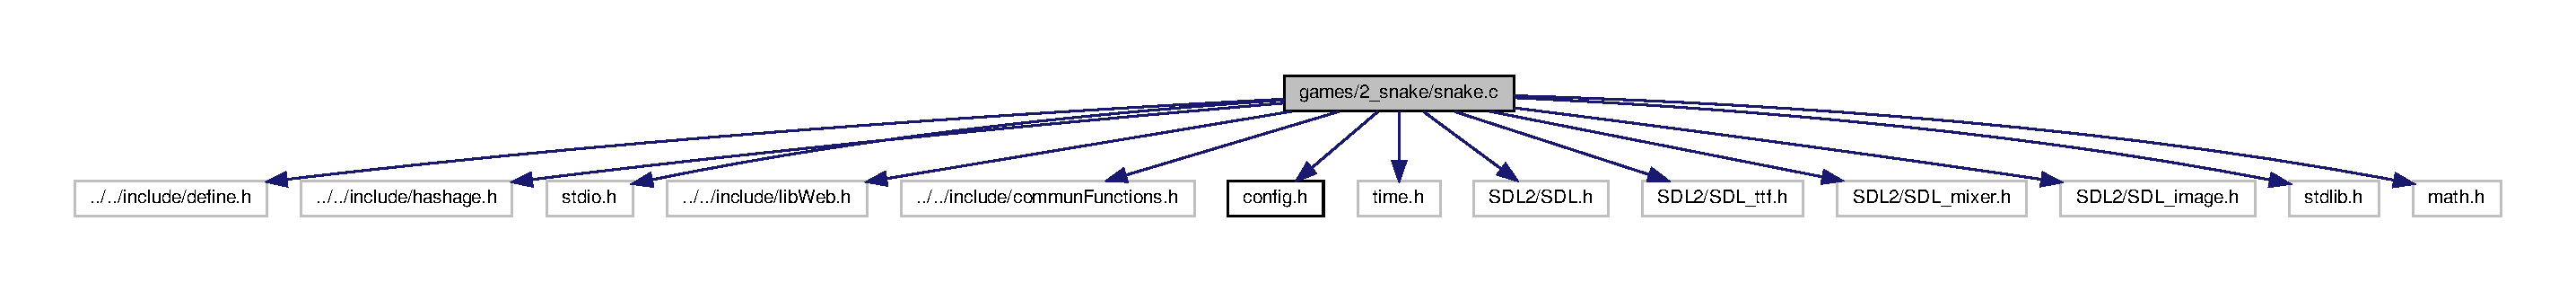
\includegraphics[width=350pt]{snake_8c__incl}
\end{center}
\end{figure}
\subsection*{Fonctions}
\begin{DoxyCompactItemize}
\item 
void \hyperlink{snake_8c_a3feffd5962865fbe7950d3bbe71ba771}{snake\+Init} ()
\begin{DoxyCompactList}\small\item\em Initialise l\textquotesingle{}environement de snake. \end{DoxyCompactList}\item 
void \hyperlink{snake_8c_a75101518da20974c59b9d79e7f740e25}{init\+Fruit} (\hyperlink{struct_fruit}{Fruit} $\ast$$\ast$fruit)
\begin{DoxyCompactList}\small\item\em Initialise le tableau dynamique de fruits. \end{DoxyCompactList}\item 
void \hyperlink{snake_8c_a4ec9d201bf0b449acfc67afdfaf10609}{init\+Bonus} (\hyperlink{struct_fruit}{Fruit} $\ast$bonus)
\begin{DoxyCompactList}\small\item\em Initialise le bonus. \end{DoxyCompactList}\item 
void \hyperlink{snake_8c_a739086fd85b17cc39593a193118b0682}{turn\+Left} (double $\ast$angle)
\begin{DoxyCompactList}\small\item\em Tourne le serpent vers la gauche. \end{DoxyCompactList}\item 
void \hyperlink{snake_8c_ae92e302f554e9e33c5a52e6251106a89}{turn\+Right} (double $\ast$angle)
\begin{DoxyCompactList}\small\item\em Tourne le serpent vers la droite. \end{DoxyCompactList}\item 
double \hyperlink{snake_8c_ae38231a62f58e817c8a5d5c0e65d81c7}{norme} (Vector2f v)
\begin{DoxyCompactList}\small\item\em Calcule la norme d\textquotesingle{}un vecteur. \end{DoxyCompactList}\item 
void \hyperlink{snake_8c_a2fa90be2b2e8c929c669e9f1d6fe57f6}{init\+Body} (size\+\_\+t $\ast$size, \hyperlink{struct_snake_part}{Snake\+Part} $\ast$$\ast$\hyperlink{snake_8c_ade7b297c3e6ac4e9ba64a21163eec9b5}{snake})
\begin{DoxyCompactList}\small\item\em Initialise le corps du serpent. \end{DoxyCompactList}\item 
void \hyperlink{snake_8c_a8daf9d3a8712f036f94adbef24b45e71}{init\+ToV} (Vector2f $\ast$v\+Tab, Vector2f v, int i\+Start, int i\+End)
\begin{DoxyCompactList}\small\item\em Initialise une portion de tableau de vecteur. \end{DoxyCompactList}\item 
void \hyperlink{snake_8c_aa7aa21dd7d83b069bbcb2cffe3bf64d2}{shift\+Refresh} (Vector2f past\+Body\mbox{[}\hyperlink{2__snake_2config_8h_affb807bf09880ade28c8c9dc7b67b71b}{R\+E\+M\+I\+N\+D\+\_\+\+B\+O\+DY}\mbox{]}, int nb\+Decale)
\begin{DoxyCompactList}\small\item\em Décale le tableau de positions anciennes du serpent pour en ajouter de nouvelles. \end{DoxyCompactList}\item 
int \hyperlink{snake_8c_ad306e9c3cf09adcb1846c4f888957eec}{add\+Body} (\hyperlink{struct_snake_part}{Snake\+Part} $\ast$$\ast$\hyperlink{snake_8c_ade7b297c3e6ac4e9ba64a21163eec9b5}{snake}, size\+\_\+t $\ast$size, Vector2f past\+Body\mbox{[}\hyperlink{2__snake_2config_8h_affb807bf09880ade28c8c9dc7b67b71b}{R\+E\+M\+I\+N\+D\+\_\+\+B\+O\+DY}\mbox{]}, float $\ast$radius\+Restant)
\begin{DoxyCompactList}\small\item\em Ajoute des parties de corps au serpent. \end{DoxyCompactList}\item 
void \hyperlink{snake_8c_aad644da8ea3e101158c01657e4f38684}{shift\+Free\+Space} (Vector2f $\ast$past\+Body)
\begin{DoxyCompactList}\small\item\em Décale le tableau de positions anciennes du serpent pour libérer de la place. \end{DoxyCompactList}\item 
void \hyperlink{snake_8c_a302fa1c00d3dfcf2e7deda97d2f86097}{shift\+Bomb} (Vector2f $\ast$past\+Body)
\begin{DoxyCompactList}\small\item\em Décale le tableau de positions anciennes du serpent lors d\textquotesingle{}une explosion de bombe. \end{DoxyCompactList}\item 
void \hyperlink{snake_8c_a24e583790e5d49a5e6fa3d179ea4ae53}{rm\+Body} (\hyperlink{struct_snake_part}{Snake\+Part} $\ast$$\ast$\hyperlink{snake_8c_ade7b297c3e6ac4e9ba64a21163eec9b5}{snake}, size\+\_\+t $\ast$size, int nb\+Rm, Vector2f $\ast$past\+Body, \hyperlink{struct_snake_part}{Snake\+Part} $\ast$$\ast$dead\+Bodies, size\+\_\+t $\ast$nb\+Dead\+Bodies, int deadly, int ratio\+Texture, int init\+Frame)
\begin{DoxyCompactList}\small\item\em Suprimme des parties du serpent. \end{DoxyCompactList}\item 
void \hyperlink{snake_8c_a0e42dbadd8f1b2e7eea7f50643e21130}{draw\+Body} (S\+D\+L\+\_\+\+Renderer $\ast$renderer, S\+D\+L\+\_\+\+Texture $\ast$snake\+Texture, \hyperlink{struct_snake_part}{Snake\+Part} $\ast$\hyperlink{snake_8c_ade7b297c3e6ac4e9ba64a21163eec9b5}{snake}, size\+\_\+t size, int frame\+Unkillable)
\begin{DoxyCompactList}\small\item\em Affiche le serpent. \end{DoxyCompactList}\item 
int \hyperlink{snake_8c_a78044bb5fe3a0f72b7777dbe1f4e2d82}{hitbox\+Tail} (\hyperlink{struct_snake_part}{Snake\+Part} $\ast$\hyperlink{snake_8c_ade7b297c3e6ac4e9ba64a21163eec9b5}{snake}, size\+\_\+t size)
\begin{DoxyCompactList}\small\item\em Détermine si la tête du serpent touche sa queue. \end{DoxyCompactList}\item 
int \hyperlink{snake_8c_aa9234d8c6419bdecdd99e4e9596fdbde}{too\+Close\+From\+Head} (\hyperlink{struct_snake_part}{Snake\+Part} head, \hyperlink{struct_fruit}{Fruit} fruit)
\begin{DoxyCompactList}\small\item\em Détermine si un fruit est trop proche de la tête pour pouvoir apparaître. \end{DoxyCompactList}\item 
static int \hyperlink{snake_8c_a88e97e8f14fe02486dcdafa98c1c1da5}{too\+Close\+From\+Wall} (Vector2f point, int dist)
\begin{DoxyCompactList}\small\item\em Détermine si un point est trop proche d\textquotesingle{}un mur par rapport à une distance donnée. \end{DoxyCompactList}\item 
int \hyperlink{snake_8c_a5ab96fad579ff79a2df0bb06e86cb7d0}{too\+Close\+From\+Corner} (\hyperlink{struct_fruit}{Fruit} fruit)
\begin{DoxyCompactList}\small\item\em Détermine si un fruit est trop proche d\textquotesingle{}un coin pour pouvoir apparaître. \end{DoxyCompactList}\item 
int \hyperlink{snake_8c_a707860ff76b3c064c97abfb3aa3562d1}{too\+Close\+From\+Fruit} (\hyperlink{struct_fruit}{Fruit} $\ast$fruit\+Rang, int rang, \hyperlink{struct_fruit}{Fruit} $\ast$fruit\+Search, int nb\+Fruit\+Search)
\begin{DoxyCompactList}\small\item\em Détermine si un fruit est trop d\textquotesingle{}un autre ou d\textquotesingle{}un bonus pour pouvoir apparaître. \end{DoxyCompactList}\item 
void \hyperlink{snake_8c_a25fd68046ffe688449023d7d4d75c95a}{spawn\+Fruit} (\hyperlink{struct_snake_part}{Snake\+Part} head, \hyperlink{struct_fruit}{Fruit} $\ast$fruit, int rang, int nb\+Fruits, float nb\+Fruit\+Eaten, \hyperlink{struct_fruit}{Fruit} $\ast$bonus, Vector2f spawn, int spawn\+Condition, int retard\+Frame, Mix\+\_\+\+Chunk $\ast$sound\+Appear, int hardcore)
\begin{DoxyCompactList}\small\item\em Fait apparaître un fruit. \end{DoxyCompactList}\item 
void \hyperlink{snake_8c_a358f322aca8a33648ffc238cd821caca}{spawn\+Bonus} (\hyperlink{struct_snake_part}{Snake\+Part} head, \hyperlink{struct_fruit}{Fruit} $\ast$bonus, float nb\+Fruit\+Eaten, \hyperlink{struct_fruit}{Fruit} $\ast$fruit, int nb\+Fruits)
\begin{DoxyCompactList}\small\item\em Fait apparaître un bonus. \end{DoxyCompactList}\item 
void \hyperlink{snake_8c_a1b081f3bfec305b13e9f0791605451c8}{reach\+Dest} (\hyperlink{struct_fruit}{Fruit} $\ast$fruit, size\+\_\+t nb\+Fruits)
\begin{DoxyCompactList}\small\item\em Déplace les fruits lors de l\textquotesingle{}animation de coffre. \end{DoxyCompactList}\item 
int \hyperlink{snake_8c_a7f4d06dd5298cf3c4dc09b54867c1b3f}{hitbox\+Fruit} (\hyperlink{struct_fruit}{Fruit} fruit, \hyperlink{struct_snake_part}{Snake\+Part} head)
\begin{DoxyCompactList}\small\item\em Détermine si la tête du serpent est sur un fruit. \end{DoxyCompactList}\item 
void \hyperlink{snake_8c_a8abf206e978ebd4f4d9ac075d0a2e01c}{draw\+Fruit} (S\+D\+L\+\_\+\+Renderer $\ast$renderer, S\+D\+L\+\_\+\+Texture $\ast$fruit\+Texture, S\+D\+L\+\_\+\+Texture $\ast$spawn\+Texture, \hyperlink{struct_fruit}{Fruit} fruit, int hardcore)
\begin{DoxyCompactList}\small\item\em Affiche un fruit. \end{DoxyCompactList}\item 
static void \hyperlink{snake_8c_a40cfb6ec79f225241ad8047cda42c6ea}{draw\+Help\+Text} (S\+D\+L\+\_\+\+Renderer $\ast$renderer, S\+D\+L\+\_\+\+Texture $\ast$fleche\+Texture)
\begin{DoxyCompactList}\small\item\em Affiche les commandes. \end{DoxyCompactList}\item 
void \hyperlink{snake_8c_a3ffbfa8da628fe1de8480152fa600f38}{draw\+Potions} (S\+D\+L\+\_\+\+Renderer $\ast$renderer, int nb\+Potion, S\+D\+L\+\_\+\+Texture $\ast$fruit\+Texture, float ratio\+Window\+Size)
\begin{DoxyCompactList}\small\item\em Affiche les potions possédés ou non. \end{DoxyCompactList}\item 
static void \hyperlink{snake_8c_ab3596b36513da05776c4e30e6e4a2cde}{draw\+Jauge} (S\+D\+L\+\_\+\+Renderer $\ast$renderer, S\+D\+L\+\_\+\+Texture $\ast$basket\+Texture, float ratio\+Window\+Size, float jauge\+Value)
\begin{DoxyCompactList}\small\item\em Affiche la jauge. \end{DoxyCompactList}\item 
void \hyperlink{snake_8c_abb567930c2685b3e7802f60895a70b62}{draw\+Dead\+Body} (S\+D\+L\+\_\+\+Renderer $\ast$renderer, S\+D\+L\+\_\+\+Texture $\ast$dead\+Body\+Texture, \hyperlink{struct_snake_part}{Snake\+Part} dead\+Body)
\begin{DoxyCompactList}\small\item\em Affiche une animation de partie de serpent morte. \end{DoxyCompactList}\item 
static void \hyperlink{snake_8c_a24a99c463dabaf629aacbc6581772e12}{draw\+Total\+Score} (S\+D\+L\+\_\+\+Renderer $\ast$renderer, T\+T\+F\+\_\+\+Font $\ast$font, int score\+Show, float ratio\+Window\+Size)
\begin{DoxyCompactList}\small\item\em Affiche une animation de partie de serpent morte. \end{DoxyCompactList}\item 
void \hyperlink{snake_8c_ac19669d13e8261ca407db47f062b9518}{shift\+Radius} (\hyperlink{struct_snake_part}{Snake\+Part} $\ast$$\ast$\hyperlink{snake_8c_ade7b297c3e6ac4e9ba64a21163eec9b5}{snake}, size\+\_\+t $\ast$size, Vector2f past\+Body\mbox{[}\hyperlink{2__snake_2config_8h_affb807bf09880ade28c8c9dc7b67b71b}{R\+E\+M\+I\+N\+D\+\_\+\+B\+O\+DY}\mbox{]}, float $\ast$radius\+Restant)
\begin{DoxyCompactList}\small\item\em Décalle la taille des parties de serpents (digestion) \end{DoxyCompactList}\item 
float \hyperlink{snake_8c_abf27e85aa2f853848d38330822cbf27b}{move\+Snake} (\hyperlink{struct_snake_part}{Snake\+Part} $\ast$$\ast$\hyperlink{snake_8c_ade7b297c3e6ac4e9ba64a21163eec9b5}{snake}, Vector2f past\+Body\mbox{[}\hyperlink{2__snake_2config_8h_affb807bf09880ade28c8c9dc7b67b71b}{R\+E\+M\+I\+N\+D\+\_\+\+B\+O\+DY}\mbox{]}, size\+\_\+t $\ast$size, float speed, double dir, \hyperlink{struct_fruit}{Fruit} $\ast$fruit, size\+\_\+t nb\+Fruits, \hyperlink{struct_fruit}{Fruit} $\ast$bonus, float $\ast$radius\+Restant, int hardcore)
\begin{DoxyCompactList}\small\item\em Décalle la taille des parties de serpents (digestion) \end{DoxyCompactList}\item 
int \hyperlink{snake_8c_a01d32a4e465831ff02093a975fc19cfc}{score\+Size} (\hyperlink{struct_fruit}{Fruit} fruit)
\begin{DoxyCompactList}\small\item\em Détermine la taille d\textquotesingle{}affichage du score d\textquotesingle{}un fruit. \end{DoxyCompactList}\item 
int \hyperlink{snake_8c_a79a3ba2cf055230de7d78992630f3acc}{eat\+Fruit} (\hyperlink{struct_snake_part}{Snake\+Part} $\ast$$\ast$\hyperlink{snake_8c_ade7b297c3e6ac4e9ba64a21163eec9b5}{snake}, size\+\_\+t $\ast$size, \hyperlink{struct_fruit}{Fruit} $\ast$$\ast$fruit\+Tab, size\+\_\+t $\ast$nb\+Fruits, \hyperlink{struct_fruit}{Fruit} fruit, float $\ast$speed, \hyperlink{struct_score_total}{Score\+Total} $\ast$score, float $\ast$nb\+Fruit\+Eaten, int $\ast$frame\+Jauge\+Anim, Vector2f $\ast$past\+Body, \hyperlink{struct_fruit}{Fruit} $\ast$bonus, \hyperlink{struct_snake_part}{Snake\+Part} $\ast$$\ast$dead\+Bodies, size\+\_\+t $\ast$nb\+Dead\+Bodies, int $\ast$nb\+Potion, float $\ast$poisoned, \hyperlink{struct_score}{Score} $\ast$$\ast$score\+Affichage, size\+\_\+t $\ast$nb\+Score\+Affichage, int $\ast$frame\+Acce, Mix\+\_\+\+Chunk $\ast$$\ast$sounds, long long $\ast$score\+\_\+hash, long keys\mbox{[}4\mbox{]}, int hardcore)
\begin{DoxyCompactList}\small\item\em Mange un fruit. \end{DoxyCompactList}\item 
static void \hyperlink{snake_8c_ad19affe43f9c0e08c2e359c5d56ed59c}{draw\+Score} (S\+D\+L\+\_\+\+Renderer $\ast$renderer, S\+D\+L\+\_\+\+Texture $\ast$score\+Texture, \hyperlink{struct_score}{Score} score\+Affichage)
\begin{DoxyCompactList}\small\item\em Affiche un score de terrain. \end{DoxyCompactList}\item 
static void \hyperlink{snake_8c_ae7a3606e921e095262b200e3b103ca87}{my\+Frees} (\hyperlink{struct_fruit}{Fruit} $\ast$$\ast$fruits, \hyperlink{struct_snake_part}{Snake\+Part} $\ast$$\ast$dead\+Bodies, \hyperlink{struct_snake_part}{Snake\+Part} $\ast$$\ast$snake\+Body, \hyperlink{struct_score}{Score} $\ast$$\ast$score\+Affichage, Mix\+\_\+\+Chunk $\ast$$\ast$sounds, S\+D\+L\+\_\+\+Texture $\ast$\hyperlink{room_8c_a158b90dfedb211efa4c317267c983dd2}{textures}\mbox{[}N\+B\+\_\+\+S\+N\+A\+K\+E\+\_\+\+T\+E\+X\+T\+U\+R\+ES\mbox{]}, T\+T\+F\+\_\+\+Font $\ast$fonts\mbox{[}\hyperlink{2__snake_2config_8h_a017842361bde423abc80e430f9777fe6}{N\+B\+\_\+\+S\+N\+A\+K\+E\+\_\+\+F\+O\+N\+TS}\mbox{]}, S\+D\+L\+\_\+\+Thread $\ast$$\ast$\hyperlink{main_8c_a584962a25015c7d6e18e294f55a8bc2d}{thread})
\begin{DoxyCompactList}\small\item\em Affiche un score de terrain. \end{DoxyCompactList}\item 
int \hyperlink{snake_8c_ade7b297c3e6ac4e9ba64a21163eec9b5}{snake} (S\+D\+L\+\_\+\+Renderer $\ast$renderer, int highscore, int \hyperlink{room_8c_a7bc33449edbe70d0faa8d9b08ac317e7}{Win\+Width}, int \hyperlink{room_8c_a14d631ded45fe3c6396d41f0b31a8aba}{Win\+Height}, char $\ast$token, int hardcore, S\+D\+L\+\_\+\+Texture $\ast$$\ast$\hyperlink{room_8c_a158b90dfedb211efa4c317267c983dd2}{textures})
\begin{DoxyCompactList}\small\item\em Affiche un score de terrain. \end{DoxyCompactList}\end{DoxyCompactItemize}
\subsection*{Variables}
\begin{DoxyCompactItemize}
\item 
int \hyperlink{snake_8c_a30862aa51c2944f287c4445751341ee8}{update\+Ended}
\end{DoxyCompactItemize}


\subsection{Description détaillée}
Jeu snake avec bonus. 

\begin{DoxyAuthor}{Auteur}
Hugo Lecomte 
\end{DoxyAuthor}
\begin{DoxyVersion}{Version}
1.\+0 
\end{DoxyVersion}
\begin{DoxyDate}{Date}
25/04/2020 
\end{DoxyDate}


\subsection{Documentation des fonctions}
\mbox{\Hypertarget{snake_8c_ad306e9c3cf09adcb1846c4f888957eec}\label{snake_8c_ad306e9c3cf09adcb1846c4f888957eec}} 
\index{snake.\+c@{snake.\+c}!add\+Body@{add\+Body}}
\index{add\+Body@{add\+Body}!snake.\+c@{snake.\+c}}
\subsubsection{\texorpdfstring{add\+Body()}{addBody()}}
{\footnotesize\ttfamily int add\+Body (\begin{DoxyParamCaption}\item[{\hyperlink{struct_snake_part}{Snake\+Part} $\ast$$\ast$}]{snake,  }\item[{size\+\_\+t $\ast$}]{size,  }\item[{Vector2f}]{past\+Body\mbox{[}\+R\+E\+M\+I\+N\+D\+\_\+\+B\+O\+D\+Y\mbox{]},  }\item[{float $\ast$}]{radius\+Restant }\end{DoxyParamCaption})}



Ajoute des parties de corps au serpent. 


\begin{DoxyParams}{Paramètres}
{\em snake} & Le tableau de parties de corps \\
\hline
{\em size} & La taille du serpent \\
\hline
{\em past\+Body} & Les positions anciennes du serpent \\
\hline
{\em radius\+Restant} & La taille excedante de la dernière partie de queue \\
\hline
\end{DoxyParams}
\begin{DoxyReturn}{Renvoie}
Le nombre de parties de corps ajoutées 
\end{DoxyReturn}
Voici le graphe d\textquotesingle{}appel pour cette fonction \+:\nopagebreak
\begin{figure}[H]
\begin{center}
\leavevmode
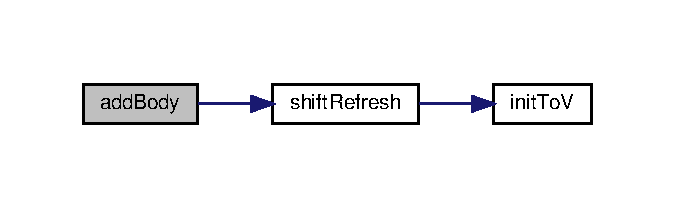
\includegraphics[width=324pt]{snake_8c_ad306e9c3cf09adcb1846c4f888957eec_cgraph}
\end{center}
\end{figure}
Voici le graphe des appelants de cette fonction \+:\nopagebreak
\begin{figure}[H]
\begin{center}
\leavevmode
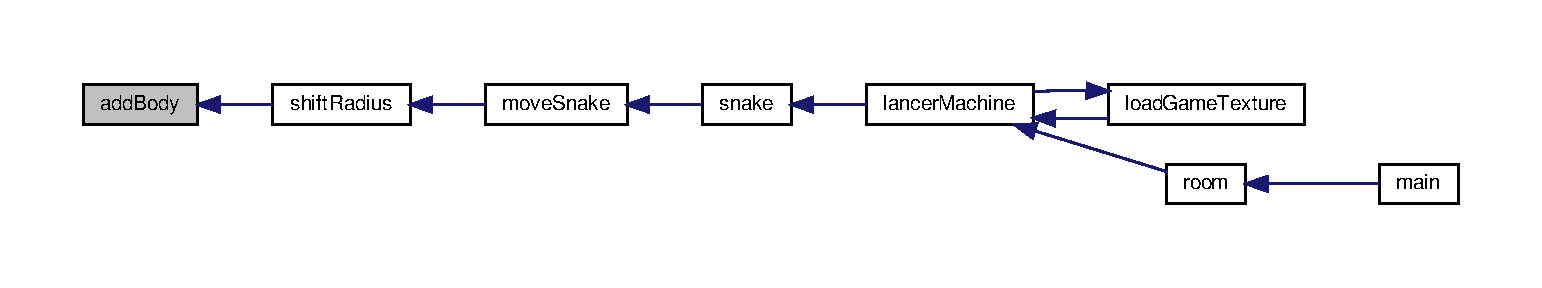
\includegraphics[width=350pt]{snake_8c_ad306e9c3cf09adcb1846c4f888957eec_icgraph}
\end{center}
\end{figure}
\mbox{\Hypertarget{snake_8c_a0e42dbadd8f1b2e7eea7f50643e21130}\label{snake_8c_a0e42dbadd8f1b2e7eea7f50643e21130}} 
\index{snake.\+c@{snake.\+c}!draw\+Body@{draw\+Body}}
\index{draw\+Body@{draw\+Body}!snake.\+c@{snake.\+c}}
\subsubsection{\texorpdfstring{draw\+Body()}{drawBody()}}
{\footnotesize\ttfamily void draw\+Body (\begin{DoxyParamCaption}\item[{S\+D\+L\+\_\+\+Renderer $\ast$}]{renderer,  }\item[{S\+D\+L\+\_\+\+Texture $\ast$}]{snake\+Texture,  }\item[{\hyperlink{struct_snake_part}{Snake\+Part} $\ast$}]{snake,  }\item[{size\+\_\+t}]{size,  }\item[{int}]{frame\+Unkillable }\end{DoxyParamCaption})}



Affiche le serpent. 


\begin{DoxyParams}{Paramètres}
{\em renderer} & Le renderer où afficher \\
\hline
{\em snake\+Texture} & La texture du serpent \\
\hline
{\em snake} & Le serpent \\
\hline
{\em size} & La taille du serpent \\
\hline
{\em frame\+Unkillable} & Le nombre de frame où le serpent est invulnérable \\
\hline
\end{DoxyParams}
Voici le graphe des appelants de cette fonction \+:\nopagebreak
\begin{figure}[H]
\begin{center}
\leavevmode
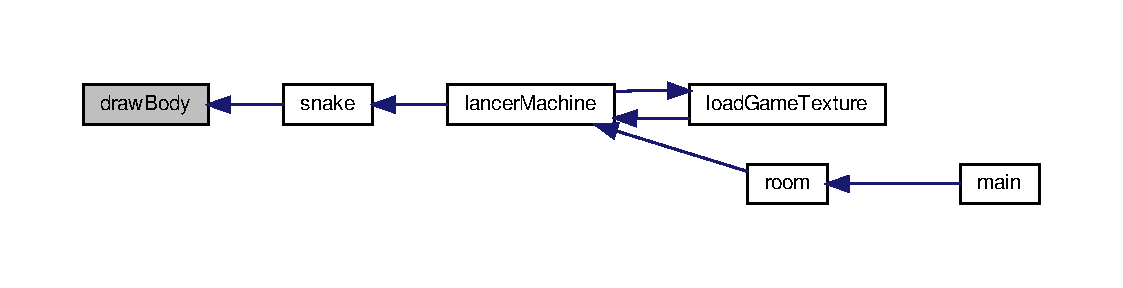
\includegraphics[width=350pt]{snake_8c_a0e42dbadd8f1b2e7eea7f50643e21130_icgraph}
\end{center}
\end{figure}
\mbox{\Hypertarget{snake_8c_abb567930c2685b3e7802f60895a70b62}\label{snake_8c_abb567930c2685b3e7802f60895a70b62}} 
\index{snake.\+c@{snake.\+c}!draw\+Dead\+Body@{draw\+Dead\+Body}}
\index{draw\+Dead\+Body@{draw\+Dead\+Body}!snake.\+c@{snake.\+c}}
\subsubsection{\texorpdfstring{draw\+Dead\+Body()}{drawDeadBody()}}
{\footnotesize\ttfamily void draw\+Dead\+Body (\begin{DoxyParamCaption}\item[{S\+D\+L\+\_\+\+Renderer $\ast$}]{renderer,  }\item[{S\+D\+L\+\_\+\+Texture $\ast$}]{dead\+Body\+Texture,  }\item[{\hyperlink{struct_snake_part}{Snake\+Part}}]{dead\+Body }\end{DoxyParamCaption})}



Affiche une animation de partie de serpent morte. 


\begin{DoxyParams}{Paramètres}
{\em renderer} & Le renderer où afficher \\
\hline
{\em dead\+Body\+Texture} & La texture d\textquotesingle{}animation de mort \\
\hline
{\em dead\+Body} & La partie morte à afficher \\
\hline
\end{DoxyParams}
Voici le graphe des appelants de cette fonction \+:\nopagebreak
\begin{figure}[H]
\begin{center}
\leavevmode
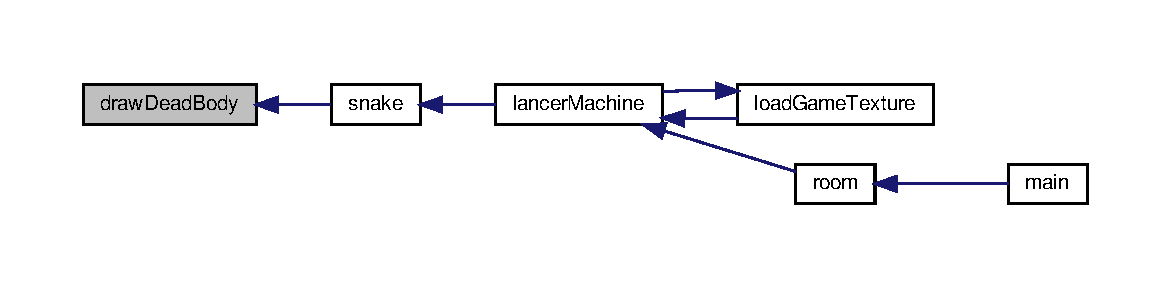
\includegraphics[width=350pt]{snake_8c_abb567930c2685b3e7802f60895a70b62_icgraph}
\end{center}
\end{figure}
\mbox{\Hypertarget{snake_8c_a8abf206e978ebd4f4d9ac075d0a2e01c}\label{snake_8c_a8abf206e978ebd4f4d9ac075d0a2e01c}} 
\index{snake.\+c@{snake.\+c}!draw\+Fruit@{draw\+Fruit}}
\index{draw\+Fruit@{draw\+Fruit}!snake.\+c@{snake.\+c}}
\subsubsection{\texorpdfstring{draw\+Fruit()}{drawFruit()}}
{\footnotesize\ttfamily void draw\+Fruit (\begin{DoxyParamCaption}\item[{S\+D\+L\+\_\+\+Renderer $\ast$}]{renderer,  }\item[{S\+D\+L\+\_\+\+Texture $\ast$}]{fruit\+Texture,  }\item[{S\+D\+L\+\_\+\+Texture $\ast$}]{spawn\+Texture,  }\item[{\hyperlink{struct_fruit}{Fruit}}]{fruit,  }\item[{int}]{hardcore }\end{DoxyParamCaption})}



Affiche un fruit. 


\begin{DoxyParams}{Paramètres}
{\em renderer} & Le renderer où afficher \\
\hline
{\em fruit\+Texture} & La texture de fruits \\
\hline
{\em spawn\+Texture} & La texture d\textquotesingle{}animation d\textquotesingle{}apparition \\
\hline
{\em fruit} & Le fruit à afficher \\
\hline
{\em hardcore} & La difficulté du jeu \\
\hline
\end{DoxyParams}
Voici le graphe des appelants de cette fonction \+:\nopagebreak
\begin{figure}[H]
\begin{center}
\leavevmode
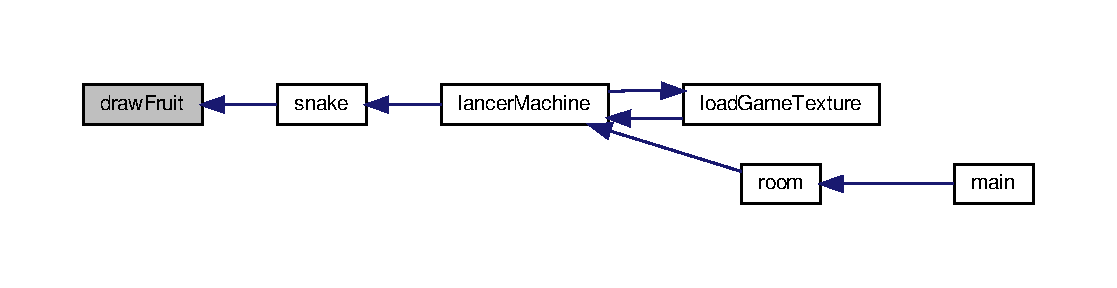
\includegraphics[width=350pt]{snake_8c_a8abf206e978ebd4f4d9ac075d0a2e01c_icgraph}
\end{center}
\end{figure}
\mbox{\Hypertarget{snake_8c_a40cfb6ec79f225241ad8047cda42c6ea}\label{snake_8c_a40cfb6ec79f225241ad8047cda42c6ea}} 
\index{snake.\+c@{snake.\+c}!draw\+Help\+Text@{draw\+Help\+Text}}
\index{draw\+Help\+Text@{draw\+Help\+Text}!snake.\+c@{snake.\+c}}
\subsubsection{\texorpdfstring{draw\+Help\+Text()}{drawHelpText()}}
{\footnotesize\ttfamily static void draw\+Help\+Text (\begin{DoxyParamCaption}\item[{S\+D\+L\+\_\+\+Renderer $\ast$}]{renderer,  }\item[{S\+D\+L\+\_\+\+Texture $\ast$}]{fleche\+Texture }\end{DoxyParamCaption})\hspace{0.3cm}{\ttfamily [static]}}



Affiche les commandes. 


\begin{DoxyParams}{Paramètres}
{\em renderer} & Le renderer où afficher \\
\hline
{\em fleche\+Texture} & La texture des flèches \\
\hline
\end{DoxyParams}
Voici le graphe des appelants de cette fonction \+:\nopagebreak
\begin{figure}[H]
\begin{center}
\leavevmode
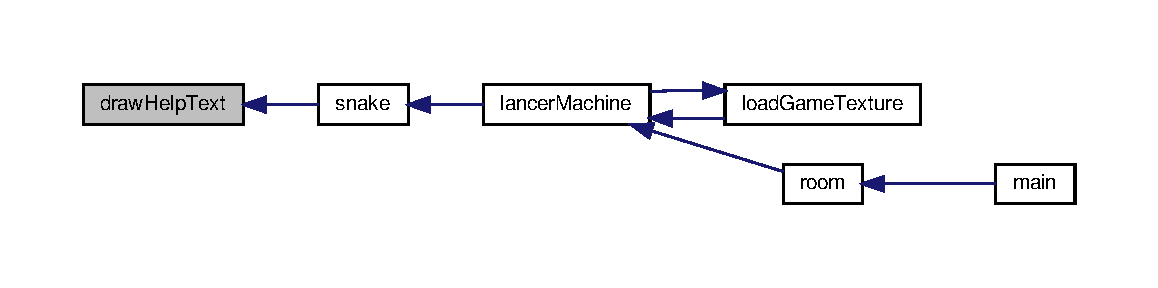
\includegraphics[width=350pt]{snake_8c_a40cfb6ec79f225241ad8047cda42c6ea_icgraph}
\end{center}
\end{figure}
\mbox{\Hypertarget{snake_8c_ab3596b36513da05776c4e30e6e4a2cde}\label{snake_8c_ab3596b36513da05776c4e30e6e4a2cde}} 
\index{snake.\+c@{snake.\+c}!draw\+Jauge@{draw\+Jauge}}
\index{draw\+Jauge@{draw\+Jauge}!snake.\+c@{snake.\+c}}
\subsubsection{\texorpdfstring{draw\+Jauge()}{drawJauge()}}
{\footnotesize\ttfamily static void draw\+Jauge (\begin{DoxyParamCaption}\item[{S\+D\+L\+\_\+\+Renderer $\ast$}]{renderer,  }\item[{S\+D\+L\+\_\+\+Texture $\ast$}]{basket\+Texture,  }\item[{float}]{ratio\+Window\+Size,  }\item[{float}]{jauge\+Value }\end{DoxyParamCaption})\hspace{0.3cm}{\ttfamily [static]}}



Affiche la jauge. 


\begin{DoxyParams}{Paramètres}
{\em renderer} & Le renderer où afficher \\
\hline
{\em basket\+Texture} & La texture de la jauge \\
\hline
{\em ratio\+Window\+Size} & Le ratio taille\+Base/taille\+Actuelle \\
\hline
{\em jauge\+Value} & La valeur de la jauge \\
\hline
\end{DoxyParams}
Voici le graphe des appelants de cette fonction \+:\nopagebreak
\begin{figure}[H]
\begin{center}
\leavevmode
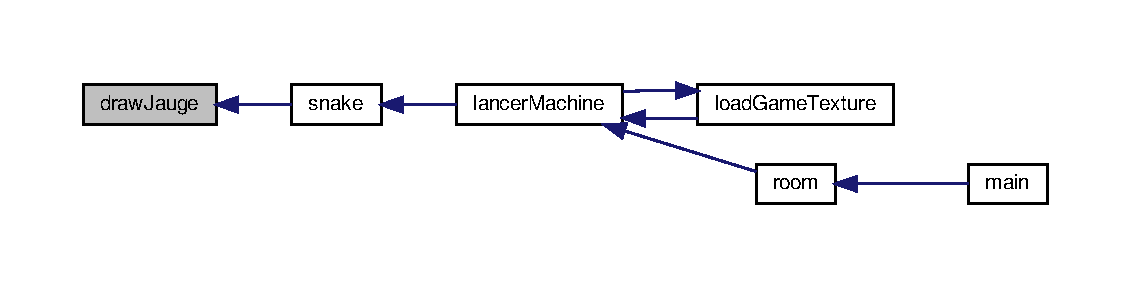
\includegraphics[width=350pt]{snake_8c_ab3596b36513da05776c4e30e6e4a2cde_icgraph}
\end{center}
\end{figure}
\mbox{\Hypertarget{snake_8c_a3ffbfa8da628fe1de8480152fa600f38}\label{snake_8c_a3ffbfa8da628fe1de8480152fa600f38}} 
\index{snake.\+c@{snake.\+c}!draw\+Potions@{draw\+Potions}}
\index{draw\+Potions@{draw\+Potions}!snake.\+c@{snake.\+c}}
\subsubsection{\texorpdfstring{draw\+Potions()}{drawPotions()}}
{\footnotesize\ttfamily void draw\+Potions (\begin{DoxyParamCaption}\item[{S\+D\+L\+\_\+\+Renderer $\ast$}]{renderer,  }\item[{int}]{nb\+Potion,  }\item[{S\+D\+L\+\_\+\+Texture $\ast$}]{fruit\+Texture,  }\item[{float}]{ratio\+Window\+Size }\end{DoxyParamCaption})}



Affiche les potions possédés ou non. 


\begin{DoxyParams}{Paramètres}
{\em renderer} & Le renderer où afficher \\
\hline
{\em nb\+Potion} & Le nombre de potions \\
\hline
{\em fruit\+Texture} & La texture des fruits \\
\hline
{\em ratio\+Window\+Size} & Le ratio taille\+Base/taille\+Actuelle \\
\hline
\end{DoxyParams}
Voici le graphe des appelants de cette fonction \+:\nopagebreak
\begin{figure}[H]
\begin{center}
\leavevmode
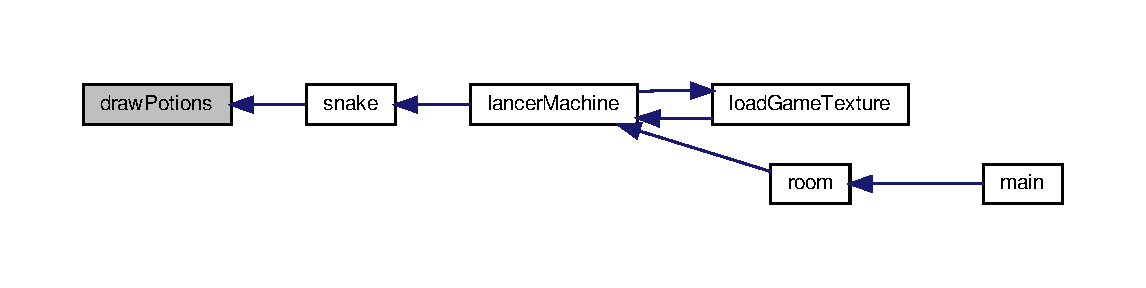
\includegraphics[width=350pt]{snake_8c_a3ffbfa8da628fe1de8480152fa600f38_icgraph}
\end{center}
\end{figure}
\mbox{\Hypertarget{snake_8c_ad19affe43f9c0e08c2e359c5d56ed59c}\label{snake_8c_ad19affe43f9c0e08c2e359c5d56ed59c}} 
\index{snake.\+c@{snake.\+c}!draw\+Score@{draw\+Score}}
\index{draw\+Score@{draw\+Score}!snake.\+c@{snake.\+c}}
\subsubsection{\texorpdfstring{draw\+Score()}{drawScore()}}
{\footnotesize\ttfamily static void draw\+Score (\begin{DoxyParamCaption}\item[{S\+D\+L\+\_\+\+Renderer $\ast$}]{renderer,  }\item[{S\+D\+L\+\_\+\+Texture $\ast$}]{score\+Texture,  }\item[{\hyperlink{struct_score}{Score}}]{score\+Affichage }\end{DoxyParamCaption})\hspace{0.3cm}{\ttfamily [static]}}



Affiche un score de terrain. 


\begin{DoxyParams}{Paramètres}
{\em renderer} & Le renderer où afficher \\
\hline
{\em score\+Texture} & La texture de score \\
\hline
{\em score\+Affichage} & Le score à afficher \\
\hline
\end{DoxyParams}
Voici le graphe d\textquotesingle{}appel pour cette fonction \+:\nopagebreak
\begin{figure}[H]
\begin{center}
\leavevmode
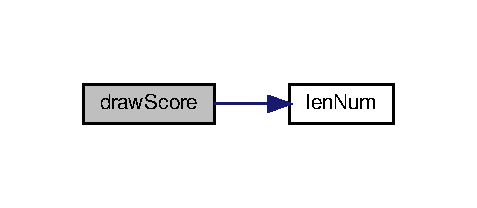
\includegraphics[width=229pt]{snake_8c_ad19affe43f9c0e08c2e359c5d56ed59c_cgraph}
\end{center}
\end{figure}
Voici le graphe des appelants de cette fonction \+:\nopagebreak
\begin{figure}[H]
\begin{center}
\leavevmode
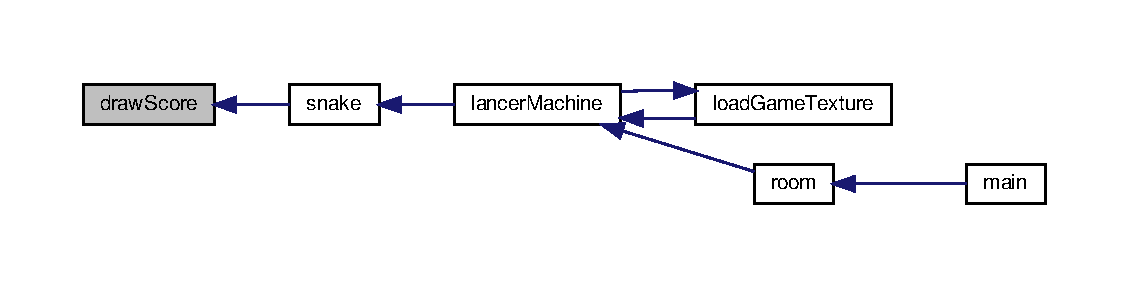
\includegraphics[width=350pt]{snake_8c_ad19affe43f9c0e08c2e359c5d56ed59c_icgraph}
\end{center}
\end{figure}
\mbox{\Hypertarget{snake_8c_a24a99c463dabaf629aacbc6581772e12}\label{snake_8c_a24a99c463dabaf629aacbc6581772e12}} 
\index{snake.\+c@{snake.\+c}!draw\+Total\+Score@{draw\+Total\+Score}}
\index{draw\+Total\+Score@{draw\+Total\+Score}!snake.\+c@{snake.\+c}}
\subsubsection{\texorpdfstring{draw\+Total\+Score()}{drawTotalScore()}}
{\footnotesize\ttfamily static void draw\+Total\+Score (\begin{DoxyParamCaption}\item[{S\+D\+L\+\_\+\+Renderer $\ast$}]{renderer,  }\item[{T\+T\+F\+\_\+\+Font $\ast$}]{font,  }\item[{int}]{score\+Show,  }\item[{float}]{ratio\+Window\+Size }\end{DoxyParamCaption})\hspace{0.3cm}{\ttfamily [static]}}



Affiche une animation de partie de serpent morte. 


\begin{DoxyParams}{Paramètres}
{\em renderer} & Le renderer où afficher \\
\hline
{\em font} & La police d\textquotesingle{}écriture \\
\hline
{\em score\+Show} & Le score total à afficher \\
\hline
{\em ratio\+Window\+Size} & Le ratio taille\+Base/taille\+Actuelle \\
\hline
\end{DoxyParams}
Voici le graphe des appelants de cette fonction \+:\nopagebreak
\begin{figure}[H]
\begin{center}
\leavevmode
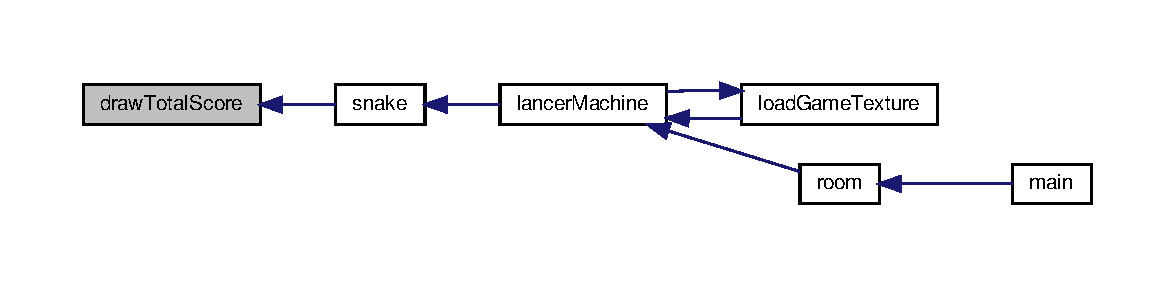
\includegraphics[width=350pt]{snake_8c_a24a99c463dabaf629aacbc6581772e12_icgraph}
\end{center}
\end{figure}
\mbox{\Hypertarget{snake_8c_a79a3ba2cf055230de7d78992630f3acc}\label{snake_8c_a79a3ba2cf055230de7d78992630f3acc}} 
\index{snake.\+c@{snake.\+c}!eat\+Fruit@{eat\+Fruit}}
\index{eat\+Fruit@{eat\+Fruit}!snake.\+c@{snake.\+c}}
\subsubsection{\texorpdfstring{eat\+Fruit()}{eatFruit()}}
{\footnotesize\ttfamily int eat\+Fruit (\begin{DoxyParamCaption}\item[{\hyperlink{struct_snake_part}{Snake\+Part} $\ast$$\ast$}]{snake,  }\item[{size\+\_\+t $\ast$}]{size,  }\item[{\hyperlink{struct_fruit}{Fruit} $\ast$$\ast$}]{fruit\+Tab,  }\item[{size\+\_\+t $\ast$}]{nb\+Fruits,  }\item[{\hyperlink{struct_fruit}{Fruit}}]{fruit,  }\item[{float $\ast$}]{speed,  }\item[{\hyperlink{struct_score_total}{Score\+Total} $\ast$}]{score,  }\item[{float $\ast$}]{nb\+Fruit\+Eaten,  }\item[{int $\ast$}]{frame\+Jauge\+Anim,  }\item[{Vector2f $\ast$}]{past\+Body,  }\item[{\hyperlink{struct_fruit}{Fruit} $\ast$}]{bonus,  }\item[{\hyperlink{struct_snake_part}{Snake\+Part} $\ast$$\ast$}]{dead\+Bodies,  }\item[{size\+\_\+t $\ast$}]{nb\+Dead\+Bodies,  }\item[{int $\ast$}]{nb\+Potion,  }\item[{float $\ast$}]{poisoned,  }\item[{\hyperlink{struct_score}{Score} $\ast$$\ast$}]{score\+Affichage,  }\item[{size\+\_\+t $\ast$}]{nb\+Score\+Affichage,  }\item[{int $\ast$}]{frame\+Acce,  }\item[{Mix\+\_\+\+Chunk $\ast$$\ast$}]{sounds,  }\item[{long long $\ast$}]{score\+\_\+hash,  }\item[{long}]{keys\mbox{[}4\mbox{]},  }\item[{int}]{hardcore }\end{DoxyParamCaption})}



Mange un fruit. 


\begin{DoxyParams}{Paramètres}
{\em snake} & Le serpent \\
\hline
{\em size} & La taille du serpent \\
\hline
{\em fruit\+Tab} & Les fruits \\
\hline
{\em nb\+Fruits} & Le nombre de fruits \\
\hline
{\em fruit} & Le fruit à manger \\
\hline
{\em speed} & La vitesse du serpent \\
\hline
{\em score} & Le score total \\
\hline
{\em nb\+Fruit\+Eaten} & Le nombre de fruits mangés \\
\hline
{\em frame\+Jauge\+Anim} & Le nombre de frame pour l\textquotesingle{}animation de jauge \\
\hline
{\em past\+Body} & Les anciennes positions du serpent \\
\hline
{\em bonus} & Le nonus \\
\hline
{\em dead\+Bodies} & Les animations de mort des parties du serpent \\
\hline
{\em nb\+Dead\+Bodies} & Le nombre d\textquotesingle{}animations de mort des parties du serpent \\
\hline
{\em nb\+Potion} & Le nombre de potions \\
\hline
{\em poisoned} & La quantité de poison ingéré \\
\hline
{\em score\+Affichage} & Les affichages de scores \\
\hline
{\em nb\+Score\+Affichage} & Le nombre d\textquotesingle{}affichage de scores \\
\hline
{\em frame\+Acce} & Le nombre de frame où l\textquotesingle{}accélération est forcée \\
\hline
{\em flap\+\_\+wav} & Le son de manger fruit \\
\hline
{\em score\+\_\+hash} & Le score hashé \\
\hline
{\em keys} & Les clés de hashage \\
\hline
{\em hardcore} & La difficulté du jeu \\
\hline
\end{DoxyParams}
\begin{DoxyReturn}{Renvoie}
Faux en cas de problème dans le hashage, sinon vrai 
\end{DoxyReturn}
Voici le graphe d\textquotesingle{}appel pour cette fonction \+:\nopagebreak
\begin{figure}[H]
\begin{center}
\leavevmode
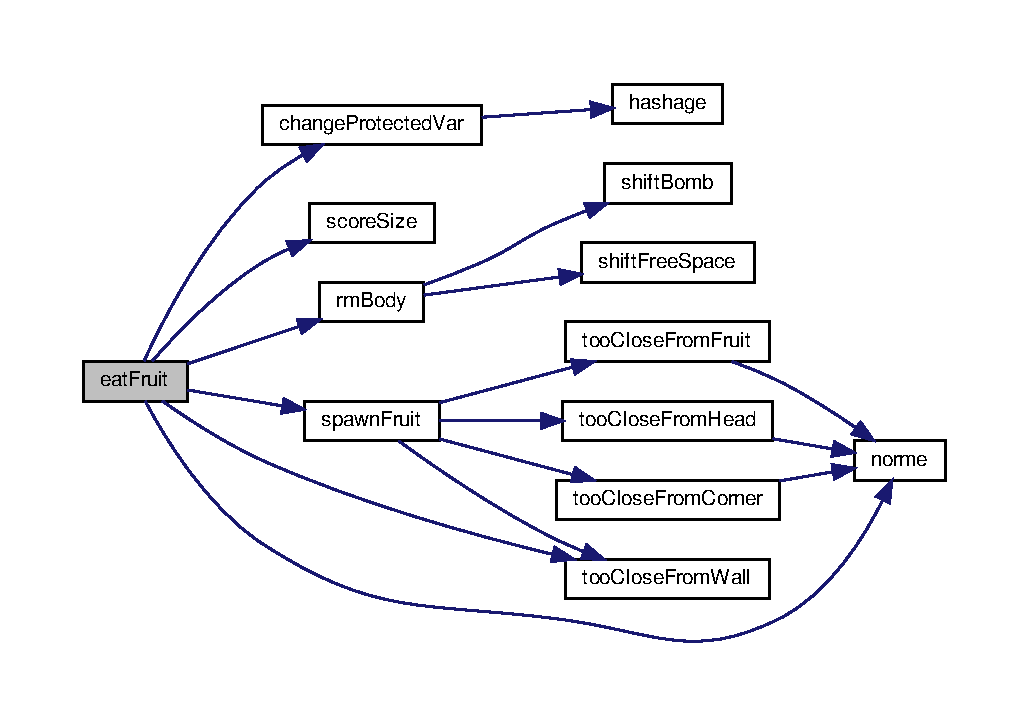
\includegraphics[width=350pt]{snake_8c_a79a3ba2cf055230de7d78992630f3acc_cgraph}
\end{center}
\end{figure}
Voici le graphe des appelants de cette fonction \+:\nopagebreak
\begin{figure}[H]
\begin{center}
\leavevmode
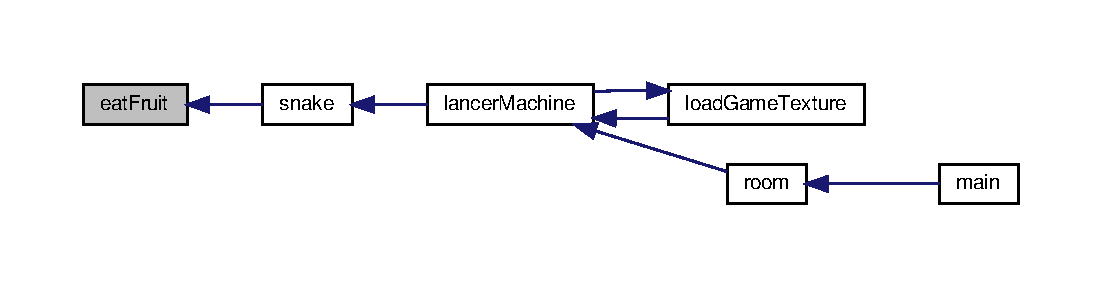
\includegraphics[width=350pt]{snake_8c_a79a3ba2cf055230de7d78992630f3acc_icgraph}
\end{center}
\end{figure}
\mbox{\Hypertarget{snake_8c_a7f4d06dd5298cf3c4dc09b54867c1b3f}\label{snake_8c_a7f4d06dd5298cf3c4dc09b54867c1b3f}} 
\index{snake.\+c@{snake.\+c}!hitbox\+Fruit@{hitbox\+Fruit}}
\index{hitbox\+Fruit@{hitbox\+Fruit}!snake.\+c@{snake.\+c}}
\subsubsection{\texorpdfstring{hitbox\+Fruit()}{hitboxFruit()}}
{\footnotesize\ttfamily int hitbox\+Fruit (\begin{DoxyParamCaption}\item[{\hyperlink{struct_fruit}{Fruit}}]{fruit,  }\item[{\hyperlink{struct_snake_part}{Snake\+Part}}]{head }\end{DoxyParamCaption})}



Détermine si la tête du serpent est sur un fruit. 


\begin{DoxyParams}{Paramètres}
{\em fruit} & Le fruit à tester \\
\hline
{\em head} & La tête du serpent \\
\hline
\end{DoxyParams}
\begin{DoxyReturn}{Renvoie}
Vrai si collision, sinon faux 
\end{DoxyReturn}
Voici le graphe d\textquotesingle{}appel pour cette fonction \+:\nopagebreak
\begin{figure}[H]
\begin{center}
\leavevmode
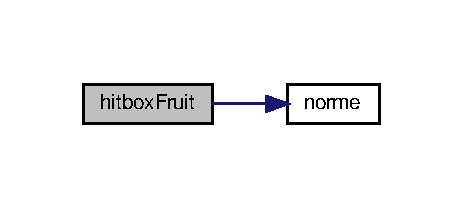
\includegraphics[width=222pt]{snake_8c_a7f4d06dd5298cf3c4dc09b54867c1b3f_cgraph}
\end{center}
\end{figure}
Voici le graphe des appelants de cette fonction \+:\nopagebreak
\begin{figure}[H]
\begin{center}
\leavevmode
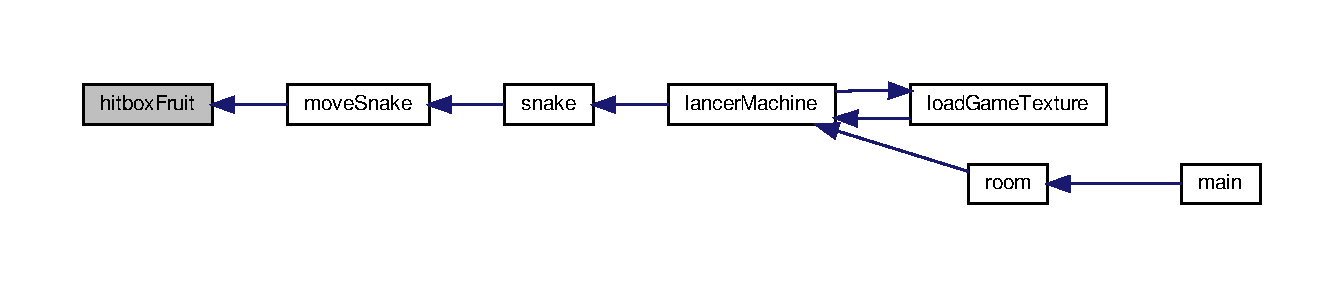
\includegraphics[width=350pt]{snake_8c_a7f4d06dd5298cf3c4dc09b54867c1b3f_icgraph}
\end{center}
\end{figure}
\mbox{\Hypertarget{snake_8c_a78044bb5fe3a0f72b7777dbe1f4e2d82}\label{snake_8c_a78044bb5fe3a0f72b7777dbe1f4e2d82}} 
\index{snake.\+c@{snake.\+c}!hitbox\+Tail@{hitbox\+Tail}}
\index{hitbox\+Tail@{hitbox\+Tail}!snake.\+c@{snake.\+c}}
\subsubsection{\texorpdfstring{hitbox\+Tail()}{hitboxTail()}}
{\footnotesize\ttfamily int hitbox\+Tail (\begin{DoxyParamCaption}\item[{\hyperlink{struct_snake_part}{Snake\+Part} $\ast$}]{snake,  }\item[{size\+\_\+t}]{size }\end{DoxyParamCaption})}



Détermine si la tête du serpent touche sa queue. 


\begin{DoxyParams}{Paramètres}
{\em snake} & Le serpent \\
\hline
{\em size} & La taille du serpent \\
\hline
\end{DoxyParams}
\begin{DoxyReturn}{Renvoie}
Vrai si il touche sa queue, sinon faux 
\end{DoxyReturn}
Voici le graphe d\textquotesingle{}appel pour cette fonction \+:\nopagebreak
\begin{figure}[H]
\begin{center}
\leavevmode
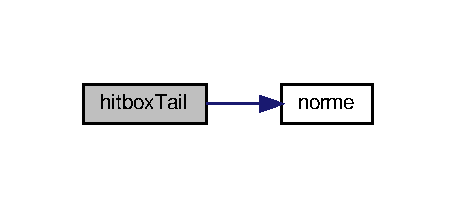
\includegraphics[width=219pt]{snake_8c_a78044bb5fe3a0f72b7777dbe1f4e2d82_cgraph}
\end{center}
\end{figure}
Voici le graphe des appelants de cette fonction \+:\nopagebreak
\begin{figure}[H]
\begin{center}
\leavevmode
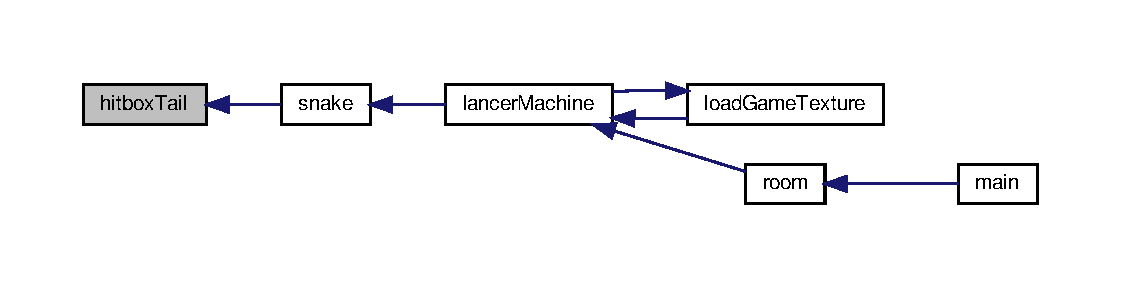
\includegraphics[width=350pt]{snake_8c_a78044bb5fe3a0f72b7777dbe1f4e2d82_icgraph}
\end{center}
\end{figure}
\mbox{\Hypertarget{snake_8c_a2fa90be2b2e8c929c669e9f1d6fe57f6}\label{snake_8c_a2fa90be2b2e8c929c669e9f1d6fe57f6}} 
\index{snake.\+c@{snake.\+c}!init\+Body@{init\+Body}}
\index{init\+Body@{init\+Body}!snake.\+c@{snake.\+c}}
\subsubsection{\texorpdfstring{init\+Body()}{initBody()}}
{\footnotesize\ttfamily void init\+Body (\begin{DoxyParamCaption}\item[{size\+\_\+t $\ast$}]{size,  }\item[{\hyperlink{struct_snake_part}{Snake\+Part} $\ast$$\ast$}]{snake }\end{DoxyParamCaption})}



Initialise le corps du serpent. 


\begin{DoxyParams}{Paramètres}
{\em size} & La taille du serpent \\
\hline
{\em snake} & Le coprs du serpent (tableau de parties de corps) \\
\hline
\end{DoxyParams}
Voici le graphe des appelants de cette fonction \+:\nopagebreak
\begin{figure}[H]
\begin{center}
\leavevmode
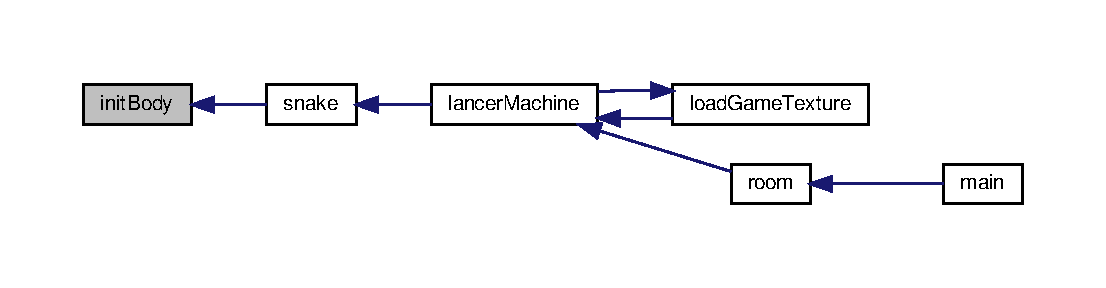
\includegraphics[width=350pt]{snake_8c_a2fa90be2b2e8c929c669e9f1d6fe57f6_icgraph}
\end{center}
\end{figure}
\mbox{\Hypertarget{snake_8c_a4ec9d201bf0b449acfc67afdfaf10609}\label{snake_8c_a4ec9d201bf0b449acfc67afdfaf10609}} 
\index{snake.\+c@{snake.\+c}!init\+Bonus@{init\+Bonus}}
\index{init\+Bonus@{init\+Bonus}!snake.\+c@{snake.\+c}}
\subsubsection{\texorpdfstring{init\+Bonus()}{initBonus()}}
{\footnotesize\ttfamily void init\+Bonus (\begin{DoxyParamCaption}\item[{\hyperlink{struct_fruit}{Fruit} $\ast$}]{bonus }\end{DoxyParamCaption})}



Initialise le bonus. 


\begin{DoxyParams}{Paramètres}
{\em bonus} & Le bonus à initialise \\
\hline
\end{DoxyParams}
Voici le graphe des appelants de cette fonction \+:\nopagebreak
\begin{figure}[H]
\begin{center}
\leavevmode
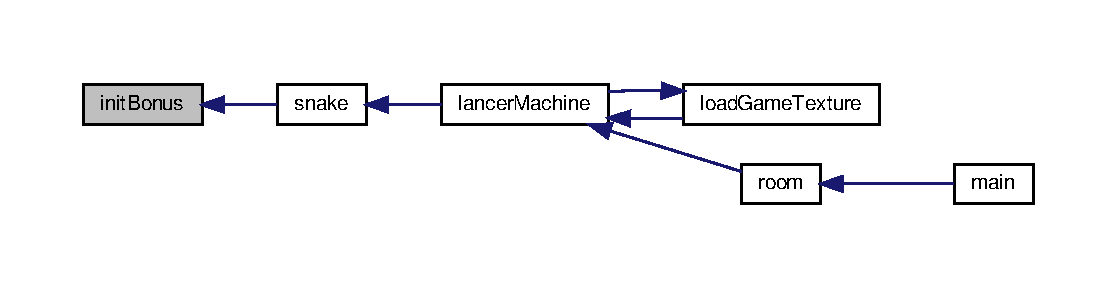
\includegraphics[width=350pt]{snake_8c_a4ec9d201bf0b449acfc67afdfaf10609_icgraph}
\end{center}
\end{figure}
\mbox{\Hypertarget{snake_8c_a75101518da20974c59b9d79e7f740e25}\label{snake_8c_a75101518da20974c59b9d79e7f740e25}} 
\index{snake.\+c@{snake.\+c}!init\+Fruit@{init\+Fruit}}
\index{init\+Fruit@{init\+Fruit}!snake.\+c@{snake.\+c}}
\subsubsection{\texorpdfstring{init\+Fruit()}{initFruit()}}
{\footnotesize\ttfamily void init\+Fruit (\begin{DoxyParamCaption}\item[{\hyperlink{struct_fruit}{Fruit} $\ast$$\ast$}]{fruit }\end{DoxyParamCaption})}



Initialise le tableau dynamique de fruits. 


\begin{DoxyParams}{Paramètres}
{\em fruit} & Le tableau dynamique de fruits \\
\hline
\end{DoxyParams}
Voici le graphe des appelants de cette fonction \+:\nopagebreak
\begin{figure}[H]
\begin{center}
\leavevmode
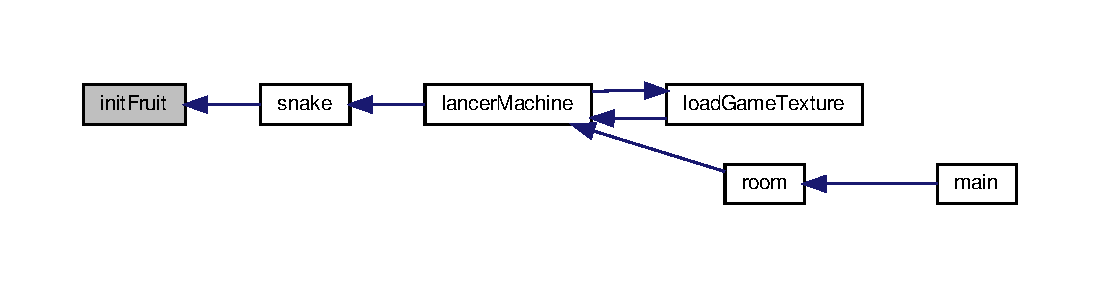
\includegraphics[width=350pt]{snake_8c_a75101518da20974c59b9d79e7f740e25_icgraph}
\end{center}
\end{figure}
\mbox{\Hypertarget{snake_8c_a8daf9d3a8712f036f94adbef24b45e71}\label{snake_8c_a8daf9d3a8712f036f94adbef24b45e71}} 
\index{snake.\+c@{snake.\+c}!init\+ToV@{init\+ToV}}
\index{init\+ToV@{init\+ToV}!snake.\+c@{snake.\+c}}
\subsubsection{\texorpdfstring{init\+To\+V()}{initToV()}}
{\footnotesize\ttfamily void init\+ToV (\begin{DoxyParamCaption}\item[{Vector2f $\ast$}]{v\+Tab,  }\item[{Vector2f}]{v,  }\item[{int}]{i\+Start,  }\item[{int}]{i\+End }\end{DoxyParamCaption})}



Initialise une portion de tableau de vecteur. 


\begin{DoxyParams}{Paramètres}
{\em v\+Tab} & Le tableau de vecteur \\
\hline
{\em v} & Le vecteur pour l\textquotesingle{}initialisation \\
\hline
{\em i\+Start} & Le premier indice du tableau à initialiser (inclus) \\
\hline
{\em i\+End} & Le dernier indice du tableau à initialiser (exclus) \\
\hline
\end{DoxyParams}
Voici le graphe des appelants de cette fonction \+:\nopagebreak
\begin{figure}[H]
\begin{center}
\leavevmode
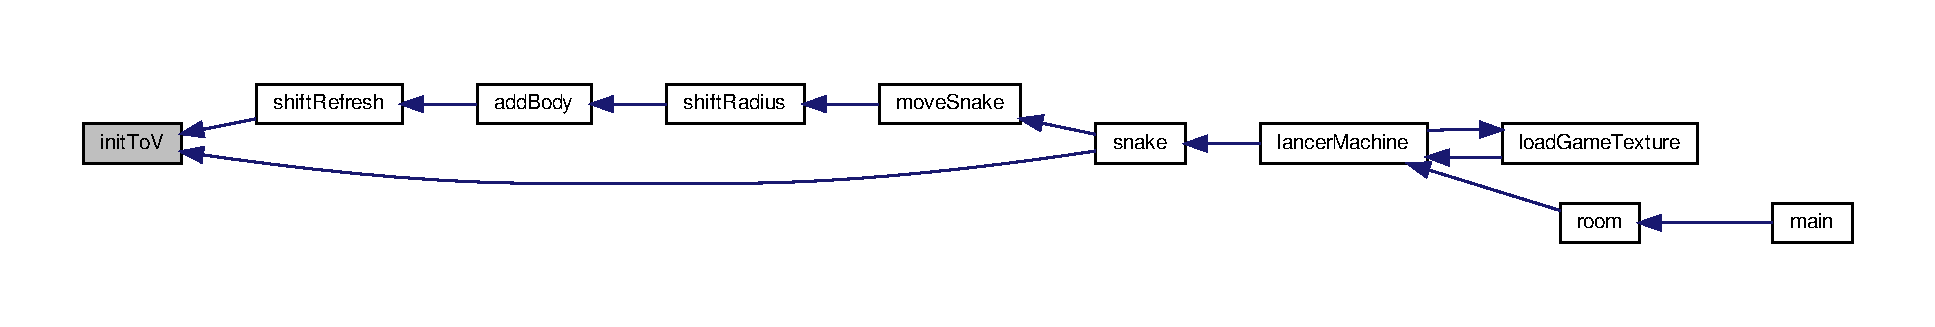
\includegraphics[width=350pt]{snake_8c_a8daf9d3a8712f036f94adbef24b45e71_icgraph}
\end{center}
\end{figure}
\mbox{\Hypertarget{snake_8c_abf27e85aa2f853848d38330822cbf27b}\label{snake_8c_abf27e85aa2f853848d38330822cbf27b}} 
\index{snake.\+c@{snake.\+c}!move\+Snake@{move\+Snake}}
\index{move\+Snake@{move\+Snake}!snake.\+c@{snake.\+c}}
\subsubsection{\texorpdfstring{move\+Snake()}{moveSnake()}}
{\footnotesize\ttfamily float move\+Snake (\begin{DoxyParamCaption}\item[{\hyperlink{struct_snake_part}{Snake\+Part} $\ast$$\ast$}]{snake,  }\item[{Vector2f}]{past\+Body\mbox{[}\+R\+E\+M\+I\+N\+D\+\_\+\+B\+O\+D\+Y\mbox{]},  }\item[{size\+\_\+t $\ast$}]{size,  }\item[{float}]{speed,  }\item[{double}]{dir,  }\item[{\hyperlink{struct_fruit}{Fruit} $\ast$}]{fruit,  }\item[{size\+\_\+t}]{nb\+Fruits,  }\item[{\hyperlink{struct_fruit}{Fruit} $\ast$}]{bonus,  }\item[{float $\ast$}]{radius\+Restant,  }\item[{int}]{hardcore }\end{DoxyParamCaption})}



Décalle la taille des parties de serpents (digestion) 


\begin{DoxyParams}{Paramètres}
{\em snake} & Le serpent \\
\hline
{\em past\+Body} & Les anciennes positions du serpent \\
\hline
{\em size} & La taille du serpent \\
\hline
{\em speed} & La vitesse du serpent \\
\hline
{\em dir} & La direction du serpent \\
\hline
{\em fruit} & Le tableau de fruits \\
\hline
{\em nb\+Fruits} & Le nombre de fruits \\
\hline
{\em bonus} & Le bonus \\
\hline
{\em radius\+Restant} & La taille de la dernière partie de la queue du serpent \\
\hline
{\em hardcore} & La difficulté du jeu \\
\hline
\end{DoxyParams}
\begin{DoxyReturn}{Renvoie}
La distance qui n\textquotesingle{}a pas été parcourue 
\end{DoxyReturn}
Voici le graphe d\textquotesingle{}appel pour cette fonction \+:\nopagebreak
\begin{figure}[H]
\begin{center}
\leavevmode
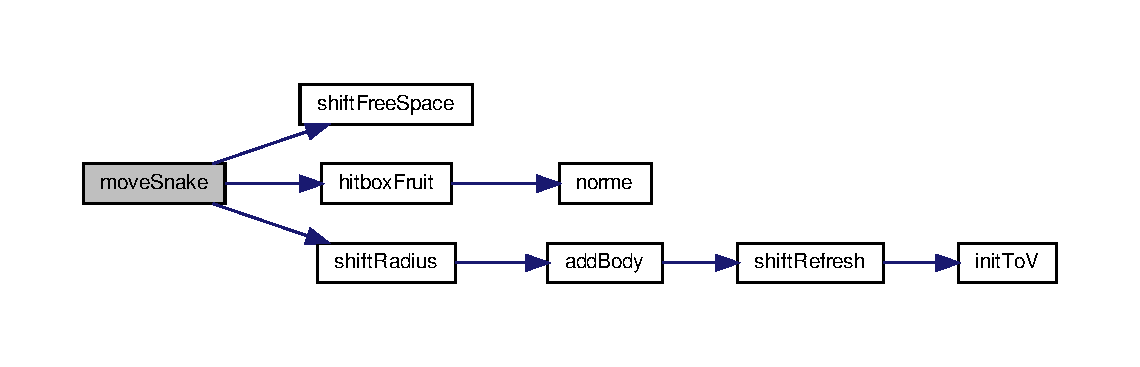
\includegraphics[width=350pt]{snake_8c_abf27e85aa2f853848d38330822cbf27b_cgraph}
\end{center}
\end{figure}
Voici le graphe des appelants de cette fonction \+:\nopagebreak
\begin{figure}[H]
\begin{center}
\leavevmode
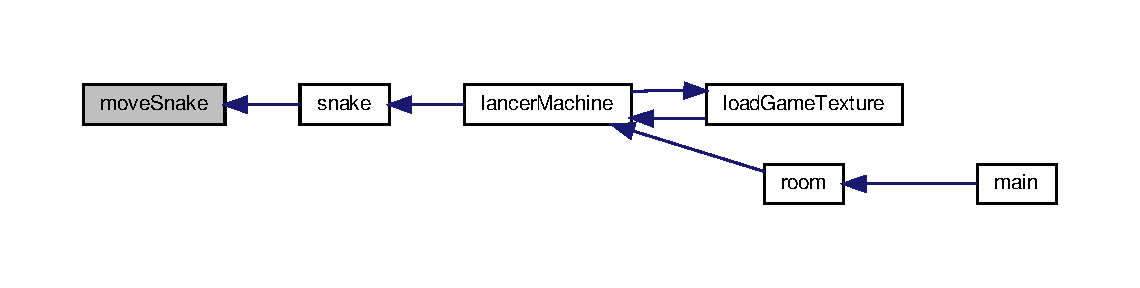
\includegraphics[width=350pt]{snake_8c_abf27e85aa2f853848d38330822cbf27b_icgraph}
\end{center}
\end{figure}
\mbox{\Hypertarget{snake_8c_ae7a3606e921e095262b200e3b103ca87}\label{snake_8c_ae7a3606e921e095262b200e3b103ca87}} 
\index{snake.\+c@{snake.\+c}!my\+Frees@{my\+Frees}}
\index{my\+Frees@{my\+Frees}!snake.\+c@{snake.\+c}}
\subsubsection{\texorpdfstring{my\+Frees()}{myFrees()}}
{\footnotesize\ttfamily static void my\+Frees (\begin{DoxyParamCaption}\item[{\hyperlink{struct_fruit}{Fruit} $\ast$$\ast$}]{fruits,  }\item[{\hyperlink{struct_snake_part}{Snake\+Part} $\ast$$\ast$}]{dead\+Bodies,  }\item[{\hyperlink{struct_snake_part}{Snake\+Part} $\ast$$\ast$}]{snake\+Body,  }\item[{\hyperlink{struct_score}{Score} $\ast$$\ast$}]{score\+Affichage,  }\item[{Mix\+\_\+\+Chunk $\ast$$\ast$}]{sounds,  }\item[{S\+D\+L\+\_\+\+Texture $\ast$}]{textures\mbox{[}\+N\+B\+\_\+\+S\+N\+A\+K\+E\+\_\+\+T\+E\+X\+T\+U\+R\+E\+S\mbox{]},  }\item[{T\+T\+F\+\_\+\+Font $\ast$}]{fonts\mbox{[}\+N\+B\+\_\+\+S\+N\+A\+K\+E\+\_\+\+F\+O\+N\+T\+S\mbox{]},  }\item[{S\+D\+L\+\_\+\+Thread $\ast$$\ast$}]{thread }\end{DoxyParamCaption})\hspace{0.3cm}{\ttfamily [static]}}



Affiche un score de terrain. 


\begin{DoxyParams}{Paramètres}
{\em fruits} & Le tableau de fruits \\
\hline
{\em dead\+Bodies} & Le tableau de parties de serpent mortes \\
\hline
{\em snake\+Body} & Le tableau de parties de serpent \\
\hline
{\em score\+Affichage} & Le tableau de score à afficher \\
\hline
{\em sound} & Le tableau de sons \\
\hline
{\em textures} & Le tableau de textures \\
\hline
{\em fonts} & Le tableau de polices \\
\hline
{\em thread} & Le thread \\
\hline
\end{DoxyParams}
Voici le graphe des appelants de cette fonction \+:\nopagebreak
\begin{figure}[H]
\begin{center}
\leavevmode
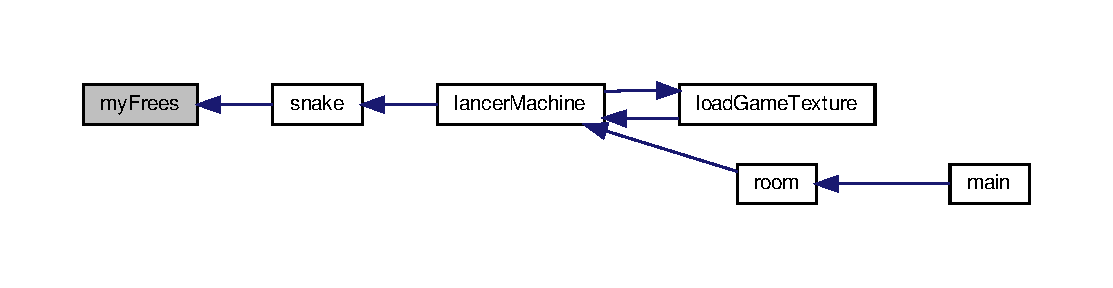
\includegraphics[width=350pt]{snake_8c_ae7a3606e921e095262b200e3b103ca87_icgraph}
\end{center}
\end{figure}
\mbox{\Hypertarget{snake_8c_ae38231a62f58e817c8a5d5c0e65d81c7}\label{snake_8c_ae38231a62f58e817c8a5d5c0e65d81c7}} 
\index{snake.\+c@{snake.\+c}!norme@{norme}}
\index{norme@{norme}!snake.\+c@{snake.\+c}}
\subsubsection{\texorpdfstring{norme()}{norme()}}
{\footnotesize\ttfamily double norme (\begin{DoxyParamCaption}\item[{Vector2f}]{v }\end{DoxyParamCaption})}



Calcule la norme d\textquotesingle{}un vecteur. 


\begin{DoxyParams}{Paramètres}
{\em v} & Le vecteur \\
\hline
\end{DoxyParams}
\begin{DoxyReturn}{Renvoie}
La norme de ce vecteur 
\end{DoxyReturn}
Voici le graphe des appelants de cette fonction \+:\nopagebreak
\begin{figure}[H]
\begin{center}
\leavevmode
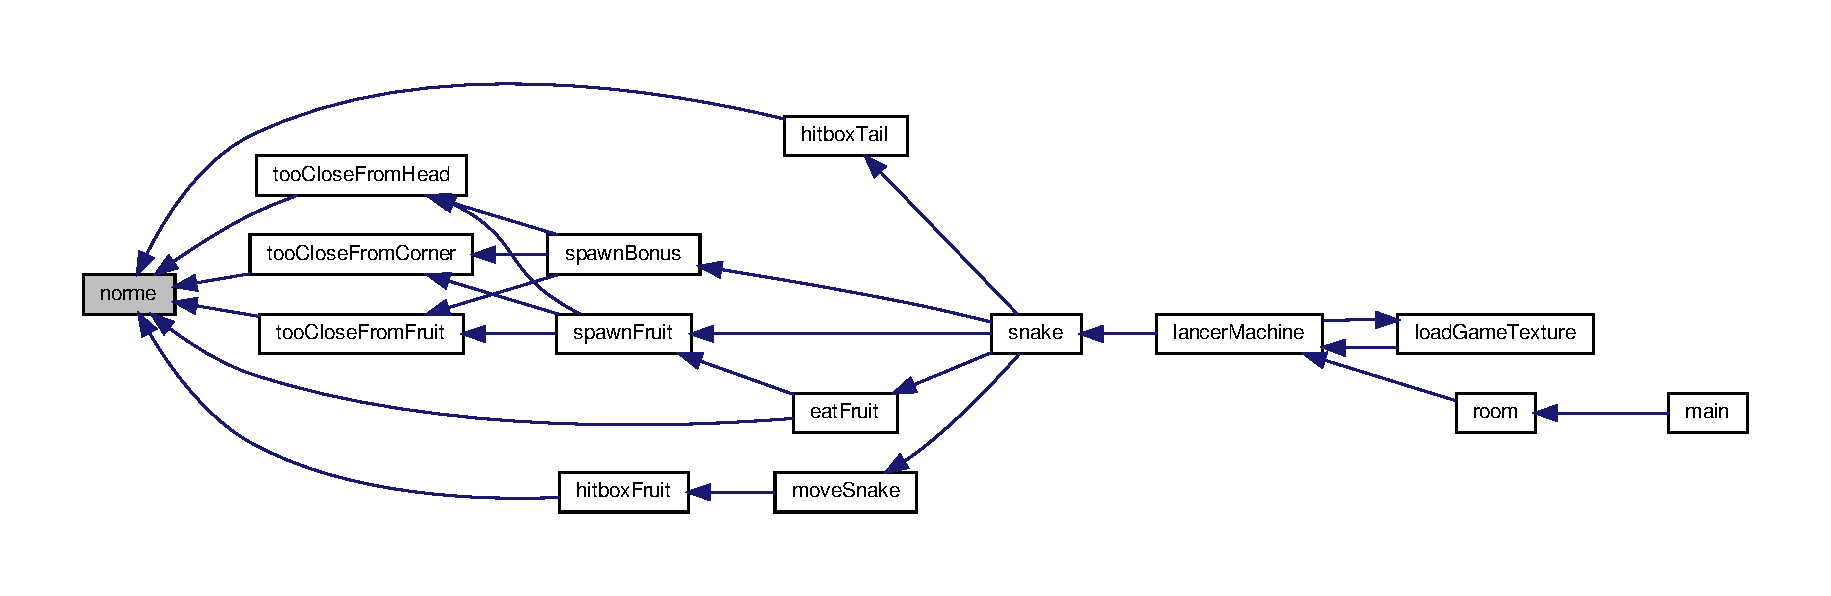
\includegraphics[width=350pt]{snake_8c_ae38231a62f58e817c8a5d5c0e65d81c7_icgraph}
\end{center}
\end{figure}
\mbox{\Hypertarget{snake_8c_a1b081f3bfec305b13e9f0791605451c8}\label{snake_8c_a1b081f3bfec305b13e9f0791605451c8}} 
\index{snake.\+c@{snake.\+c}!reach\+Dest@{reach\+Dest}}
\index{reach\+Dest@{reach\+Dest}!snake.\+c@{snake.\+c}}
\subsubsection{\texorpdfstring{reach\+Dest()}{reachDest()}}
{\footnotesize\ttfamily void reach\+Dest (\begin{DoxyParamCaption}\item[{\hyperlink{struct_fruit}{Fruit} $\ast$}]{fruit,  }\item[{size\+\_\+t}]{nb\+Fruits }\end{DoxyParamCaption})}



Déplace les fruits lors de l\textquotesingle{}animation de coffre. 


\begin{DoxyParams}{Paramètres}
{\em fruit} & Le tableau de fruits \\
\hline
{\em nb\+Fruits} & Le nombre de fruits mangés (réduit par les fruits expirés) \\
\hline
\end{DoxyParams}
Voici le graphe des appelants de cette fonction \+:\nopagebreak
\begin{figure}[H]
\begin{center}
\leavevmode
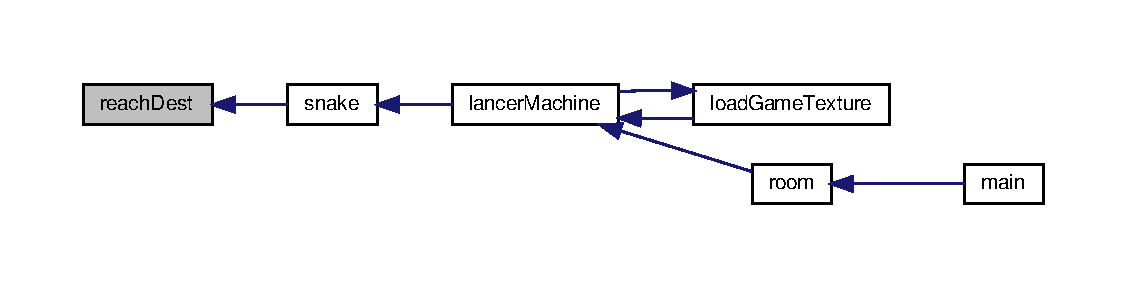
\includegraphics[width=350pt]{snake_8c_a1b081f3bfec305b13e9f0791605451c8_icgraph}
\end{center}
\end{figure}
\mbox{\Hypertarget{snake_8c_a24e583790e5d49a5e6fa3d179ea4ae53}\label{snake_8c_a24e583790e5d49a5e6fa3d179ea4ae53}} 
\index{snake.\+c@{snake.\+c}!rm\+Body@{rm\+Body}}
\index{rm\+Body@{rm\+Body}!snake.\+c@{snake.\+c}}
\subsubsection{\texorpdfstring{rm\+Body()}{rmBody()}}
{\footnotesize\ttfamily void rm\+Body (\begin{DoxyParamCaption}\item[{\hyperlink{struct_snake_part}{Snake\+Part} $\ast$$\ast$}]{snake,  }\item[{size\+\_\+t $\ast$}]{size,  }\item[{int}]{nb\+Rm,  }\item[{Vector2f $\ast$}]{past\+Body,  }\item[{\hyperlink{struct_snake_part}{Snake\+Part} $\ast$$\ast$}]{dead\+Bodies,  }\item[{size\+\_\+t $\ast$}]{nb\+Dead\+Bodies,  }\item[{int}]{deadly,  }\item[{int}]{ratio\+Texture,  }\item[{int}]{init\+Frame }\end{DoxyParamCaption})}



Suprimme des parties du serpent. 


\begin{DoxyParams}{Paramètres}
{\em snake} & Le serpent \\
\hline
{\em size} & La taille du serpent \\
\hline
{\em nb\+Rm} & Le nombre de parties à supprimer \\
\hline
{\em past\+Body} & Le tableau de positions anciennes \\
\hline
{\em dead\+Bodies} & Le tableau de parties de serpent détruites \\
\hline
{\em nb\+Dead\+Bodies} & Le nombre de parties de serpent détruites \\
\hline
{\em deadly} & Détermine si cette supression peut tuer le serpent \\
\hline
{\em ratio\+Texture} & Détermine tous les combien de parties supprimées il faut afficher l\textquotesingle{}animation \\
\hline
{\em init\+Frame} & Détermine combien de parties sont passées sans afficher d\textquotesingle{}animation de mort de partie de serpent (animation de mort) \\
\hline
\end{DoxyParams}
Voici le graphe d\textquotesingle{}appel pour cette fonction \+:\nopagebreak
\begin{figure}[H]
\begin{center}
\leavevmode
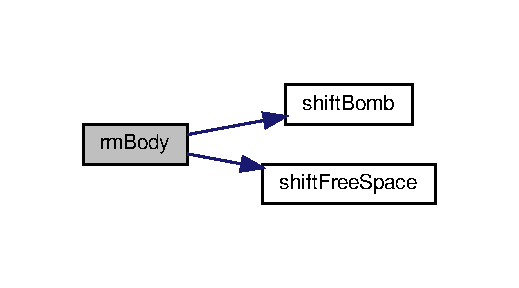
\includegraphics[width=249pt]{snake_8c_a24e583790e5d49a5e6fa3d179ea4ae53_cgraph}
\end{center}
\end{figure}
Voici le graphe des appelants de cette fonction \+:\nopagebreak
\begin{figure}[H]
\begin{center}
\leavevmode
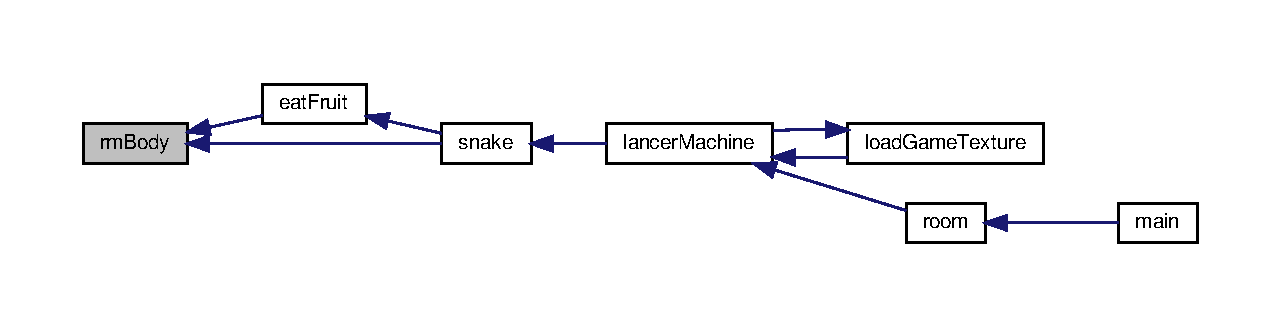
\includegraphics[width=350pt]{snake_8c_a24e583790e5d49a5e6fa3d179ea4ae53_icgraph}
\end{center}
\end{figure}
\mbox{\Hypertarget{snake_8c_a01d32a4e465831ff02093a975fc19cfc}\label{snake_8c_a01d32a4e465831ff02093a975fc19cfc}} 
\index{snake.\+c@{snake.\+c}!score\+Size@{score\+Size}}
\index{score\+Size@{score\+Size}!snake.\+c@{snake.\+c}}
\subsubsection{\texorpdfstring{score\+Size()}{scoreSize()}}
{\footnotesize\ttfamily int score\+Size (\begin{DoxyParamCaption}\item[{\hyperlink{struct_fruit}{Fruit}}]{fruit }\end{DoxyParamCaption})}



Détermine la taille d\textquotesingle{}affichage du score d\textquotesingle{}un fruit. 


\begin{DoxyParams}{Paramètres}
{\em fruit} & Le fruit \\
\hline
\end{DoxyParams}
\begin{DoxyReturn}{Renvoie}
Sa taille d\textquotesingle{}affichage de score 
\end{DoxyReturn}
Voici le graphe des appelants de cette fonction \+:\nopagebreak
\begin{figure}[H]
\begin{center}
\leavevmode
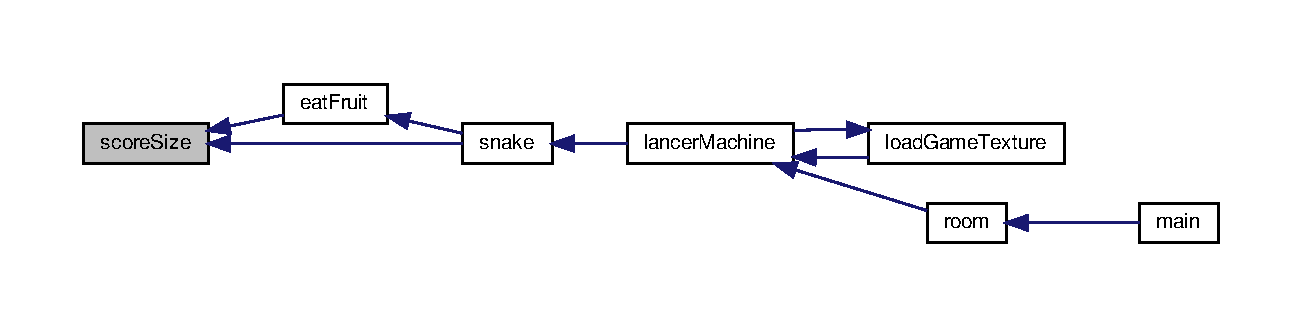
\includegraphics[width=350pt]{snake_8c_a01d32a4e465831ff02093a975fc19cfc_icgraph}
\end{center}
\end{figure}
\mbox{\Hypertarget{snake_8c_a302fa1c00d3dfcf2e7deda97d2f86097}\label{snake_8c_a302fa1c00d3dfcf2e7deda97d2f86097}} 
\index{snake.\+c@{snake.\+c}!shift\+Bomb@{shift\+Bomb}}
\index{shift\+Bomb@{shift\+Bomb}!snake.\+c@{snake.\+c}}
\subsubsection{\texorpdfstring{shift\+Bomb()}{shiftBomb()}}
{\footnotesize\ttfamily void shift\+Bomb (\begin{DoxyParamCaption}\item[{Vector2f $\ast$}]{past\+Body }\end{DoxyParamCaption})}



Décale le tableau de positions anciennes du serpent lors d\textquotesingle{}une explosion de bombe. 


\begin{DoxyParams}{Paramètres}
{\em past\+Body} & Le tableau de positions anciennes \\
\hline
\end{DoxyParams}
Voici le graphe des appelants de cette fonction \+:\nopagebreak
\begin{figure}[H]
\begin{center}
\leavevmode
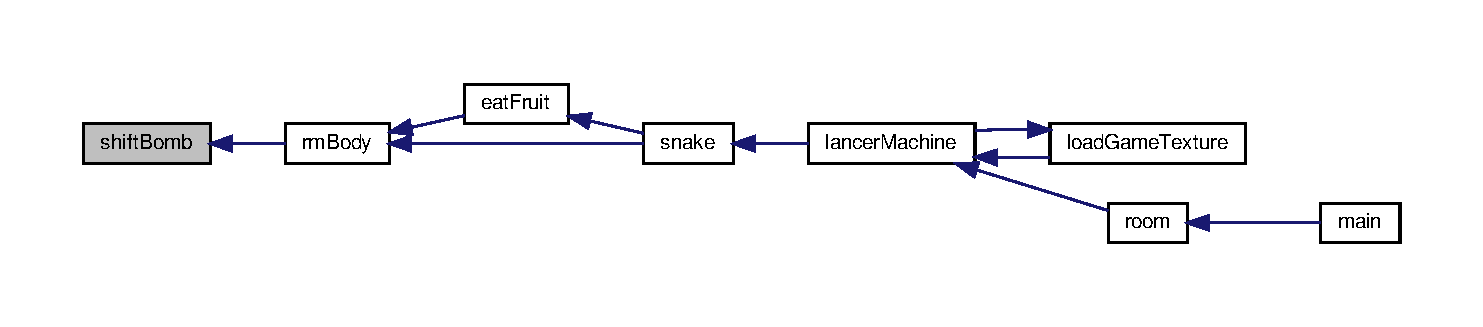
\includegraphics[width=350pt]{snake_8c_a302fa1c00d3dfcf2e7deda97d2f86097_icgraph}
\end{center}
\end{figure}
\mbox{\Hypertarget{snake_8c_aad644da8ea3e101158c01657e4f38684}\label{snake_8c_aad644da8ea3e101158c01657e4f38684}} 
\index{snake.\+c@{snake.\+c}!shift\+Free\+Space@{shift\+Free\+Space}}
\index{shift\+Free\+Space@{shift\+Free\+Space}!snake.\+c@{snake.\+c}}
\subsubsection{\texorpdfstring{shift\+Free\+Space()}{shiftFreeSpace()}}
{\footnotesize\ttfamily void shift\+Free\+Space (\begin{DoxyParamCaption}\item[{Vector2f $\ast$}]{past\+Body }\end{DoxyParamCaption})}



Décale le tableau de positions anciennes du serpent pour libérer de la place. 


\begin{DoxyParams}{Paramètres}
{\em past\+Body} & Le tableau de positions anciennes \\
\hline
\end{DoxyParams}
Voici le graphe des appelants de cette fonction \+:\nopagebreak
\begin{figure}[H]
\begin{center}
\leavevmode
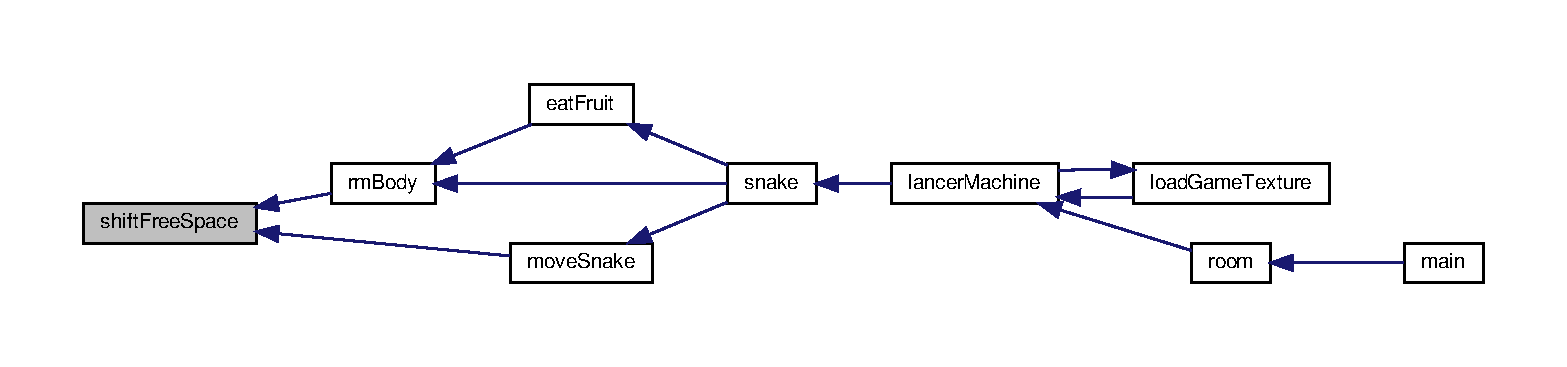
\includegraphics[width=350pt]{snake_8c_aad644da8ea3e101158c01657e4f38684_icgraph}
\end{center}
\end{figure}
\mbox{\Hypertarget{snake_8c_ac19669d13e8261ca407db47f062b9518}\label{snake_8c_ac19669d13e8261ca407db47f062b9518}} 
\index{snake.\+c@{snake.\+c}!shift\+Radius@{shift\+Radius}}
\index{shift\+Radius@{shift\+Radius}!snake.\+c@{snake.\+c}}
\subsubsection{\texorpdfstring{shift\+Radius()}{shiftRadius()}}
{\footnotesize\ttfamily void shift\+Radius (\begin{DoxyParamCaption}\item[{\hyperlink{struct_snake_part}{Snake\+Part} $\ast$$\ast$}]{snake,  }\item[{size\+\_\+t $\ast$}]{size,  }\item[{Vector2f}]{past\+Body\mbox{[}\+R\+E\+M\+I\+N\+D\+\_\+\+B\+O\+D\+Y\mbox{]},  }\item[{float $\ast$}]{radius\+Restant }\end{DoxyParamCaption})}



Décalle la taille des parties de serpents (digestion) 


\begin{DoxyParams}{Paramètres}
{\em snake} & Le serpent \\
\hline
{\em size} & La taille du serpent \\
\hline
{\em past\+Body} & Les anciennes positions du serpent \\
\hline
{\em radius\+Restant} & La taille de la dernière partie de la queue du serpent \\
\hline
\end{DoxyParams}
Voici le graphe d\textquotesingle{}appel pour cette fonction \+:\nopagebreak
\begin{figure}[H]
\begin{center}
\leavevmode
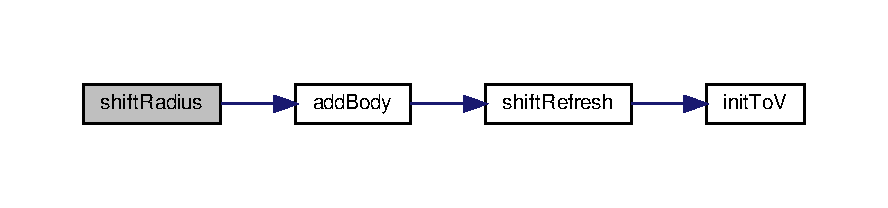
\includegraphics[width=350pt]{snake_8c_ac19669d13e8261ca407db47f062b9518_cgraph}
\end{center}
\end{figure}
Voici le graphe des appelants de cette fonction \+:\nopagebreak
\begin{figure}[H]
\begin{center}
\leavevmode
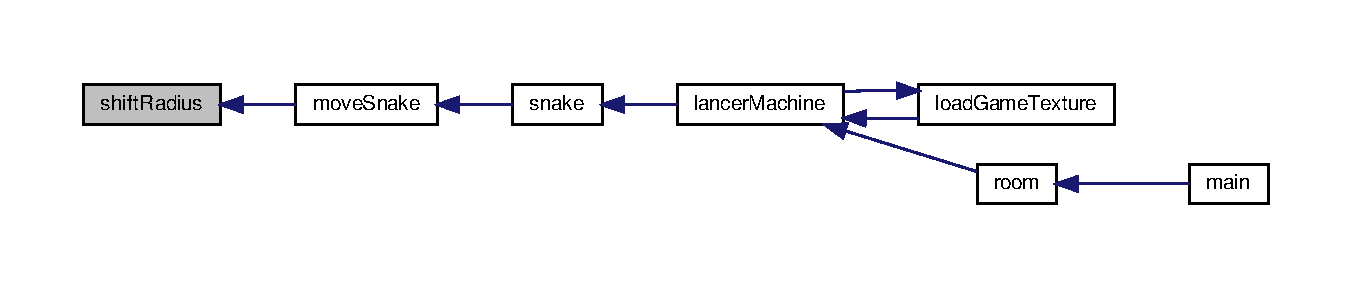
\includegraphics[width=350pt]{snake_8c_ac19669d13e8261ca407db47f062b9518_icgraph}
\end{center}
\end{figure}
\mbox{\Hypertarget{snake_8c_aa7aa21dd7d83b069bbcb2cffe3bf64d2}\label{snake_8c_aa7aa21dd7d83b069bbcb2cffe3bf64d2}} 
\index{snake.\+c@{snake.\+c}!shift\+Refresh@{shift\+Refresh}}
\index{shift\+Refresh@{shift\+Refresh}!snake.\+c@{snake.\+c}}
\subsubsection{\texorpdfstring{shift\+Refresh()}{shiftRefresh()}}
{\footnotesize\ttfamily void shift\+Refresh (\begin{DoxyParamCaption}\item[{Vector2f}]{past\+Body\mbox{[}\+R\+E\+M\+I\+N\+D\+\_\+\+B\+O\+D\+Y\mbox{]},  }\item[{int}]{nb\+Decale }\end{DoxyParamCaption})}



Décale le tableau de positions anciennes du serpent pour en ajouter de nouvelles. 


\begin{DoxyParams}{Paramètres}
{\em past\+Body} & Le tableau de positiones anciennes \\
\hline
{\em nb\+Decale} & La quantité de décalage \\
\hline
\end{DoxyParams}
Voici le graphe d\textquotesingle{}appel pour cette fonction \+:\nopagebreak
\begin{figure}[H]
\begin{center}
\leavevmode
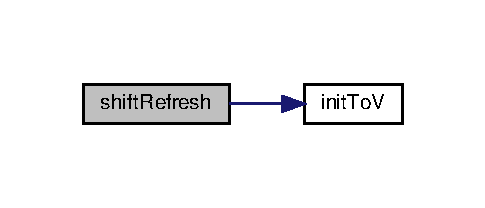
\includegraphics[width=233pt]{snake_8c_aa7aa21dd7d83b069bbcb2cffe3bf64d2_cgraph}
\end{center}
\end{figure}
Voici le graphe des appelants de cette fonction \+:\nopagebreak
\begin{figure}[H]
\begin{center}
\leavevmode
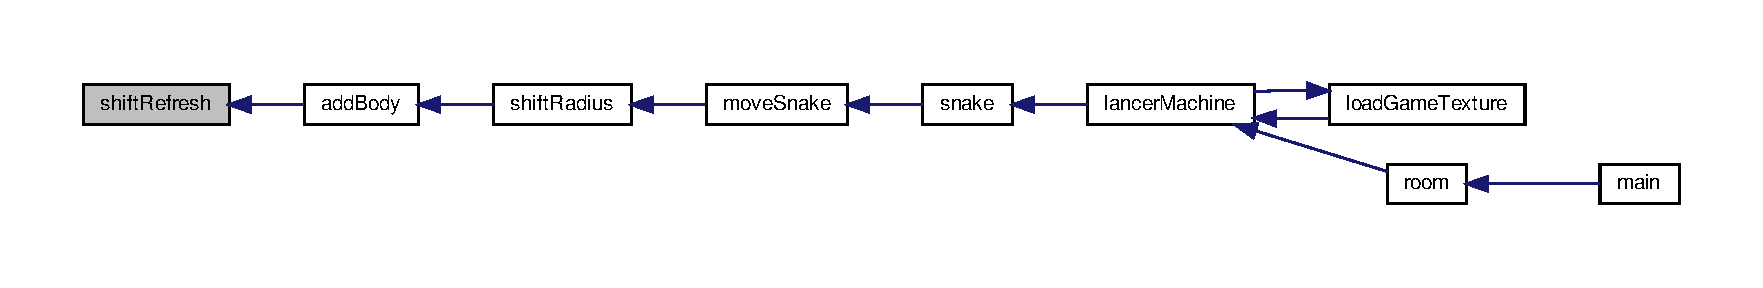
\includegraphics[width=350pt]{snake_8c_aa7aa21dd7d83b069bbcb2cffe3bf64d2_icgraph}
\end{center}
\end{figure}
\mbox{\Hypertarget{snake_8c_ade7b297c3e6ac4e9ba64a21163eec9b5}\label{snake_8c_ade7b297c3e6ac4e9ba64a21163eec9b5}} 
\index{snake.\+c@{snake.\+c}!snake@{snake}}
\index{snake@{snake}!snake.\+c@{snake.\+c}}
\subsubsection{\texorpdfstring{snake()}{snake()}}
{\footnotesize\ttfamily int snake (\begin{DoxyParamCaption}\item[{S\+D\+L\+\_\+\+Renderer $\ast$}]{renderer,  }\item[{int}]{highscore,  }\item[{int}]{Win\+Width,  }\item[{int}]{Win\+Height,  }\item[{char $\ast$}]{token,  }\item[{int}]{hardcore,  }\item[{S\+D\+L\+\_\+\+Texture $\ast$$\ast$}]{textures }\end{DoxyParamCaption})}



Affiche un score de terrain. 

$<$ Changée dans le thread pour savoir s\textquotesingle{}il est finit $>$


\begin{DoxyParams}{Paramètres}
{\em renderer} & Le renderer \\
\hline
{\em highscore} & Le meilleur score personnel \\
\hline
{\em Win\+Width} & La largeur de la fenêtre \\
\hline
{\em Win\+Height} & La hauteur de la fenêtre \\
\hline
{\em token} & Le token pour l\textquotesingle{}envoi des scores \\
\hline
{\em hardcore} & Le difficulté du jeu \\
\hline
\end{DoxyParams}
M\+I\+SE EN P\+L\+A\+CE ///``

Vars ///`

B\+O\+U\+C\+LE DU J\+EU ///``Voici le graphe d\textquotesingle{}appel pour cette fonction \+:\nopagebreak
\begin{figure}[H]
\begin{center}
\leavevmode
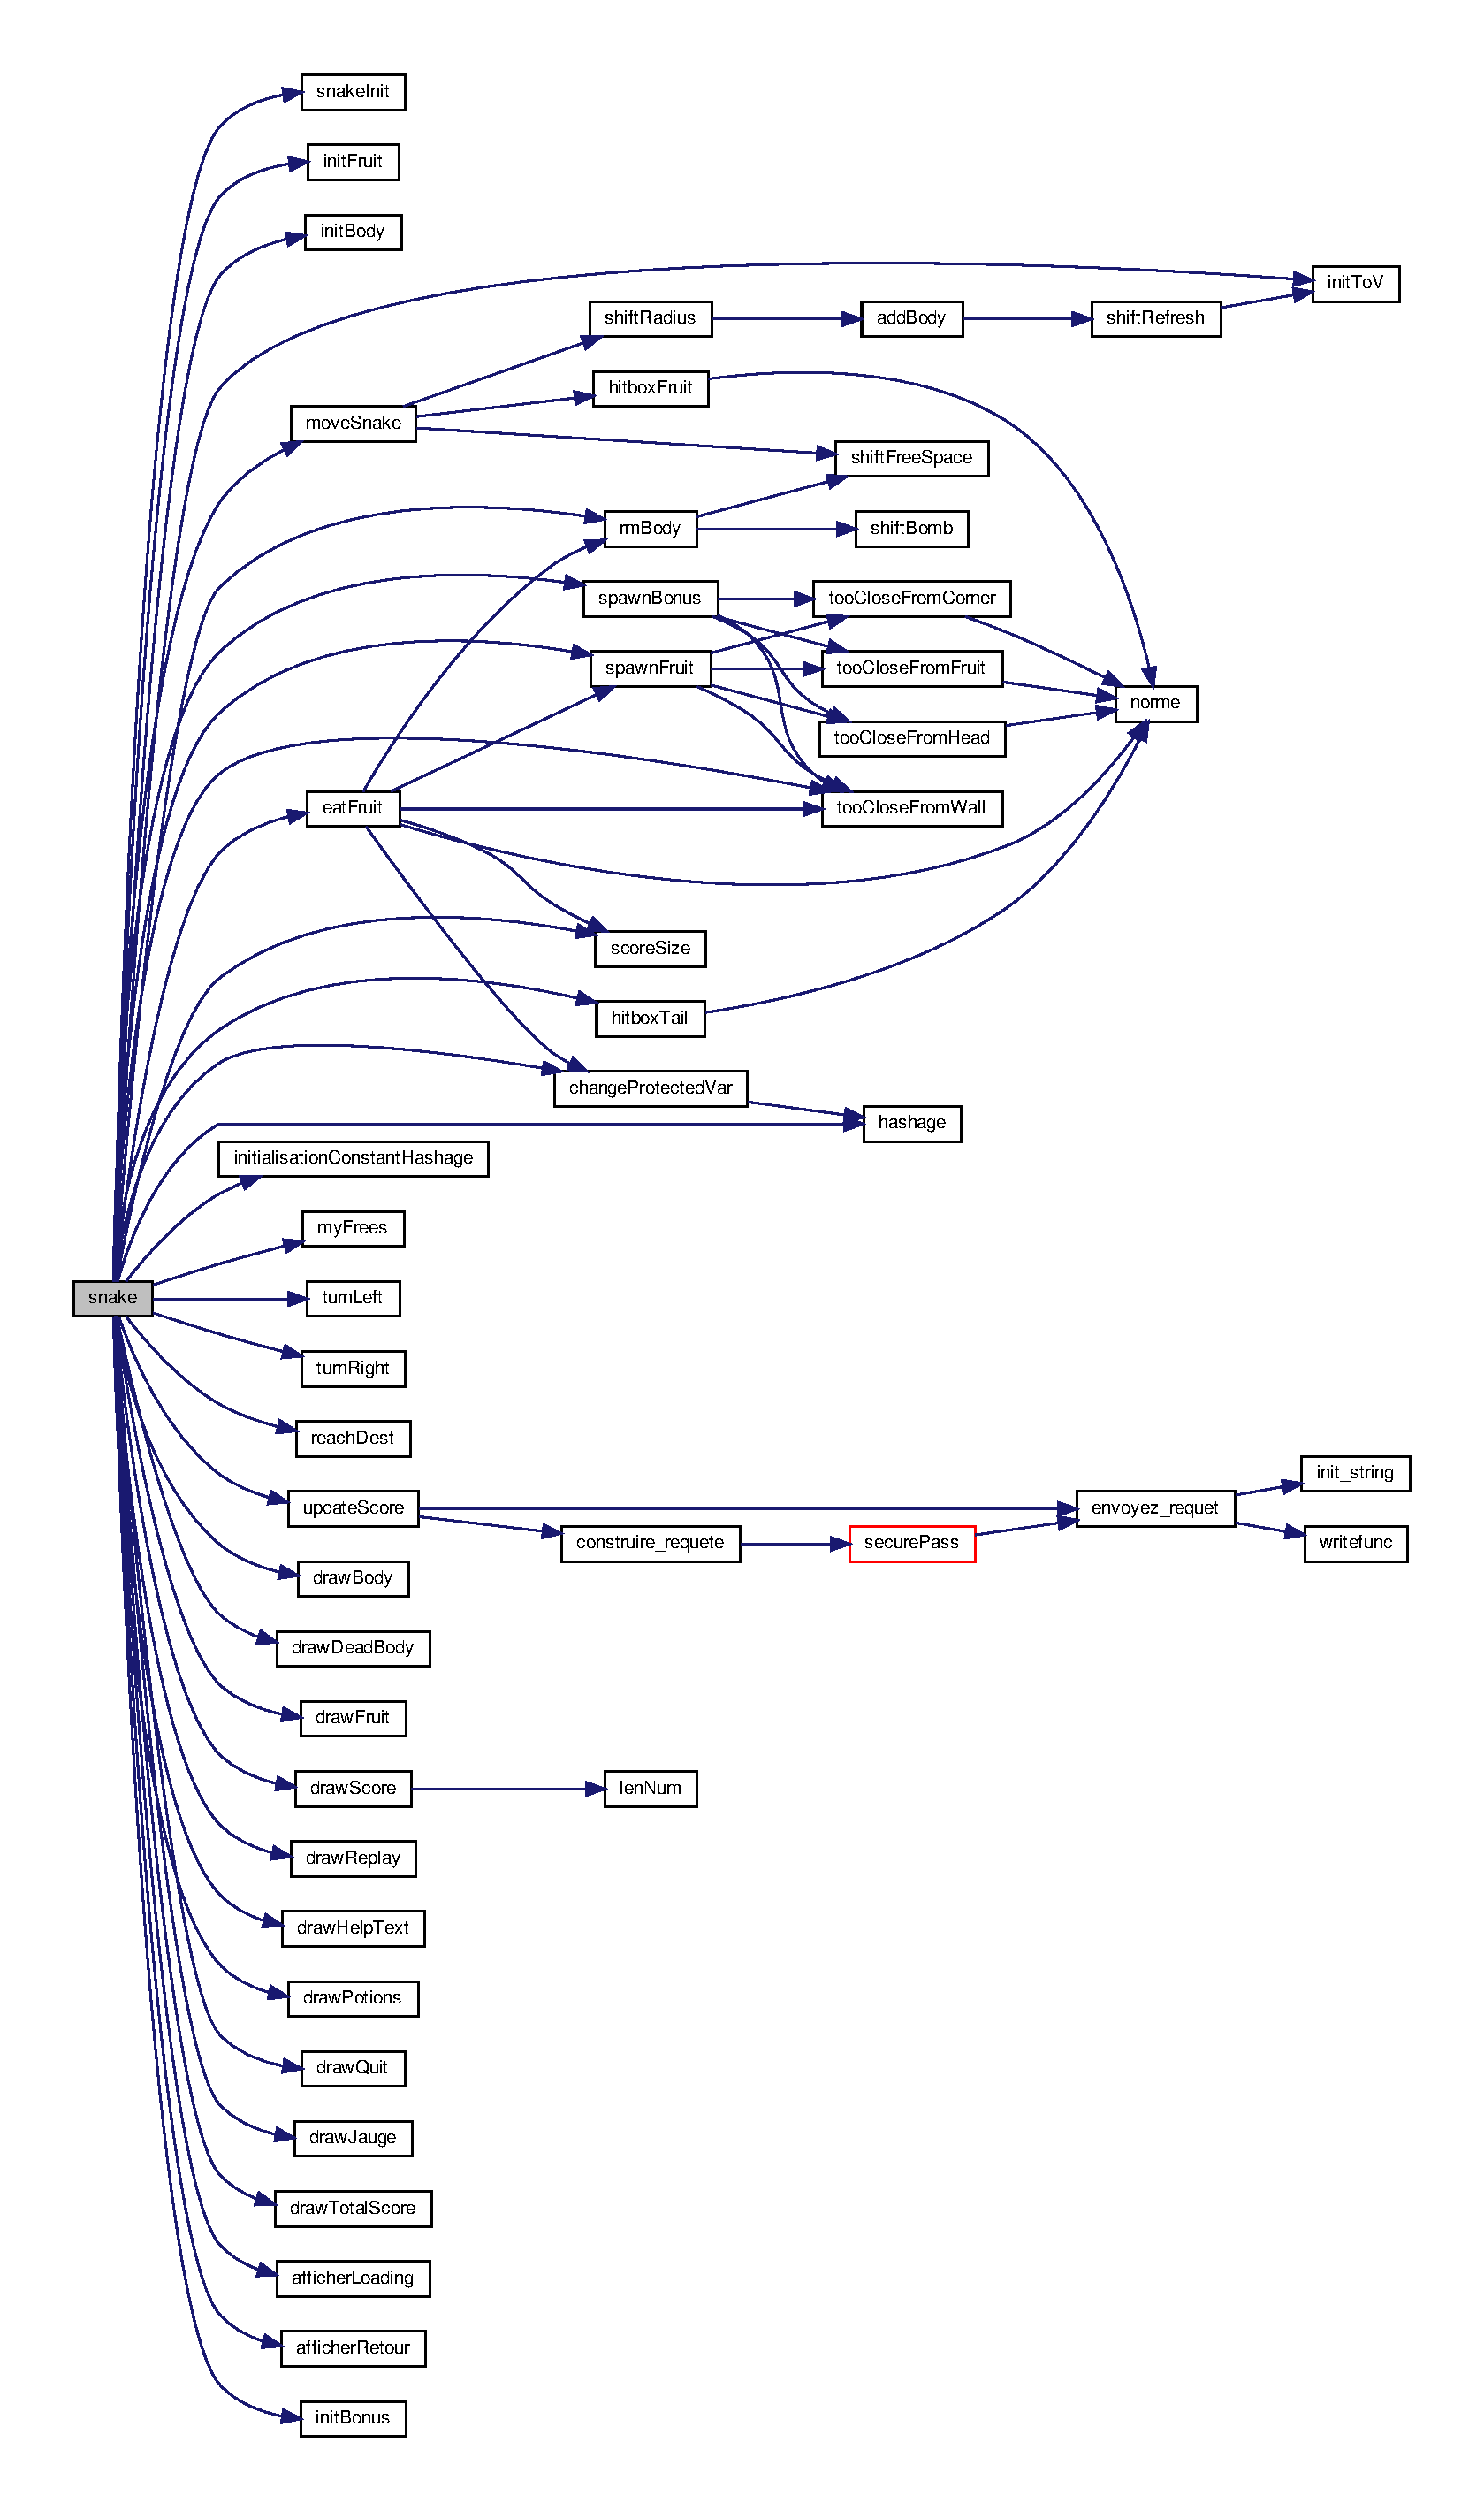
\includegraphics[height=550pt]{snake_8c_ade7b297c3e6ac4e9ba64a21163eec9b5_cgraph}
\end{center}
\end{figure}
Voici le graphe des appelants de cette fonction \+:\nopagebreak
\begin{figure}[H]
\begin{center}
\leavevmode
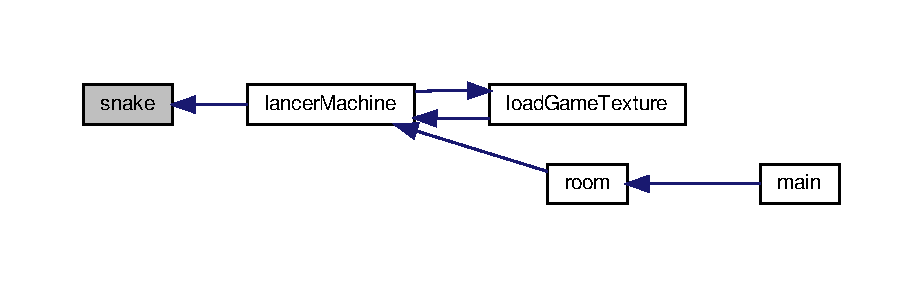
\includegraphics[width=350pt]{snake_8c_ade7b297c3e6ac4e9ba64a21163eec9b5_icgraph}
\end{center}
\end{figure}
\mbox{\Hypertarget{snake_8c_a3feffd5962865fbe7950d3bbe71ba771}\label{snake_8c_a3feffd5962865fbe7950d3bbe71ba771}} 
\index{snake.\+c@{snake.\+c}!snake\+Init@{snake\+Init}}
\index{snake\+Init@{snake\+Init}!snake.\+c@{snake.\+c}}
\subsubsection{\texorpdfstring{snake\+Init()}{snakeInit()}}
{\footnotesize\ttfamily void snake\+Init (\begin{DoxyParamCaption}{ }\end{DoxyParamCaption})}



Initialise l\textquotesingle{}environement de snake. 

Voici le graphe des appelants de cette fonction \+:\nopagebreak
\begin{figure}[H]
\begin{center}
\leavevmode
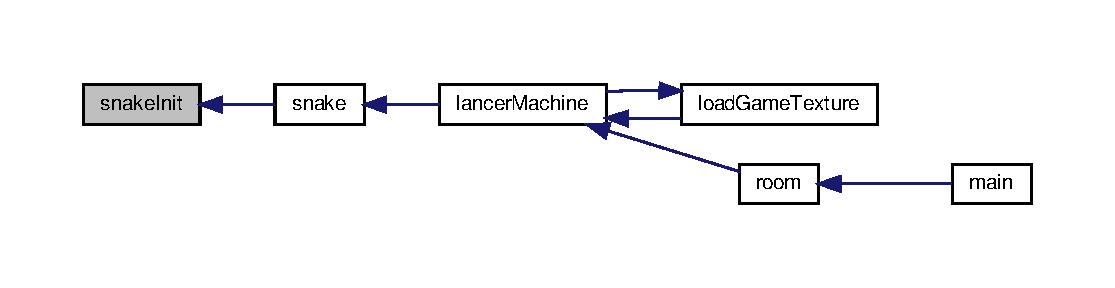
\includegraphics[width=350pt]{snake_8c_a3feffd5962865fbe7950d3bbe71ba771_icgraph}
\end{center}
\end{figure}
\mbox{\Hypertarget{snake_8c_a358f322aca8a33648ffc238cd821caca}\label{snake_8c_a358f322aca8a33648ffc238cd821caca}} 
\index{snake.\+c@{snake.\+c}!spawn\+Bonus@{spawn\+Bonus}}
\index{spawn\+Bonus@{spawn\+Bonus}!snake.\+c@{snake.\+c}}
\subsubsection{\texorpdfstring{spawn\+Bonus()}{spawnBonus()}}
{\footnotesize\ttfamily void spawn\+Bonus (\begin{DoxyParamCaption}\item[{\hyperlink{struct_snake_part}{Snake\+Part}}]{head,  }\item[{\hyperlink{struct_fruit}{Fruit} $\ast$}]{bonus,  }\item[{float}]{nb\+Fruit\+Eaten,  }\item[{\hyperlink{struct_fruit}{Fruit} $\ast$}]{fruit,  }\item[{int}]{nb\+Fruits }\end{DoxyParamCaption})}



Fait apparaître un bonus. 


\begin{DoxyParams}{Paramètres}
{\em head} & La tête du serpent \\
\hline
{\em bonus} & Le bonus \\
\hline
{\em nb\+Fruit\+Eaten} & Le nombre d\textquotesingle{}élément dans ce tableau \\
\hline
{\em fruit} & Le tableau de fruits \\
\hline
{\em nb\+Fruits} & Le nombre de fruits mangés (réduit par les fruits expirés) \\
\hline
\end{DoxyParams}
Voici le graphe d\textquotesingle{}appel pour cette fonction \+:\nopagebreak
\begin{figure}[H]
\begin{center}
\leavevmode
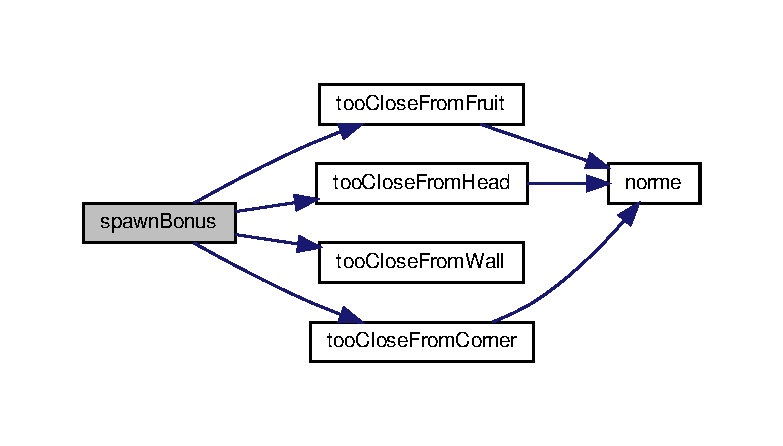
\includegraphics[width=350pt]{snake_8c_a358f322aca8a33648ffc238cd821caca_cgraph}
\end{center}
\end{figure}
Voici le graphe des appelants de cette fonction \+:\nopagebreak
\begin{figure}[H]
\begin{center}
\leavevmode
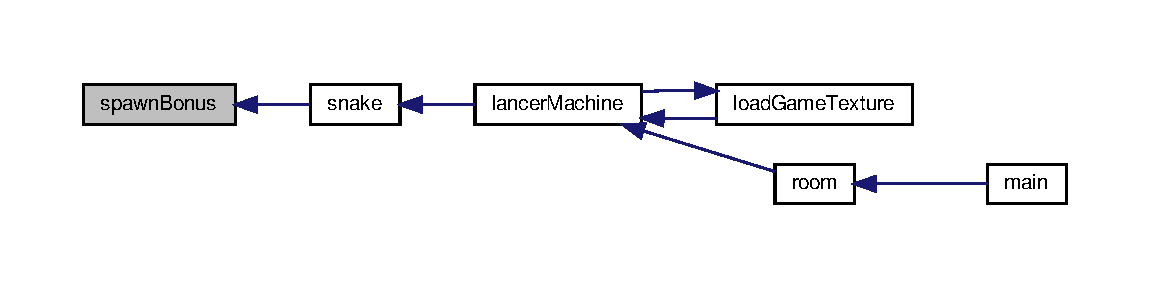
\includegraphics[width=350pt]{snake_8c_a358f322aca8a33648ffc238cd821caca_icgraph}
\end{center}
\end{figure}
\mbox{\Hypertarget{snake_8c_a25fd68046ffe688449023d7d4d75c95a}\label{snake_8c_a25fd68046ffe688449023d7d4d75c95a}} 
\index{snake.\+c@{snake.\+c}!spawn\+Fruit@{spawn\+Fruit}}
\index{spawn\+Fruit@{spawn\+Fruit}!snake.\+c@{snake.\+c}}
\subsubsection{\texorpdfstring{spawn\+Fruit()}{spawnFruit()}}
{\footnotesize\ttfamily void spawn\+Fruit (\begin{DoxyParamCaption}\item[{\hyperlink{struct_snake_part}{Snake\+Part}}]{head,  }\item[{\hyperlink{struct_fruit}{Fruit} $\ast$}]{fruit,  }\item[{int}]{rang,  }\item[{int}]{nb\+Fruits,  }\item[{float}]{nb\+Fruit\+Eaten,  }\item[{\hyperlink{struct_fruit}{Fruit} $\ast$}]{bonus,  }\item[{Vector2f}]{spawn,  }\item[{int}]{spawn\+Condition,  }\item[{int}]{retard\+Frame,  }\item[{Mix\+\_\+\+Chunk $\ast$}]{sound\+Appear,  }\item[{int}]{hardcore }\end{DoxyParamCaption})}



Fait apparaître un fruit. 


\begin{DoxyParams}{Paramètres}
{\em head} & La tête du serpent \\
\hline
{\em fruit} & Le tableau de fruit \\
\hline
{\em rang} & Le rang du fruit à faire apparaître \\
\hline
{\em nb\+Fruits} & Le nombre de fruits mangés (réduit par les fruits expirés) \\
\hline
{\em nb\+Fruit\+Eaten} & Le nombre d\textquotesingle{}élément dans ce tableau \\
\hline
{\em bonus} & Le bonus \\
\hline
{\em spawn} & La position d\textquotesingle{}apparition si elle n\textquotesingle{}est pas aléatoire \\
\hline
{\em spawn\+Condition} & La condition d\textquotesingle{}apparition ( naturelle, coffre...) \\
\hline
{\em retard\+Frame} & Le nombre de frame avant que l\textquotesingle{}apparition du fruit commence \\
\hline
{\em sound\+Appear} & Le son d\textquotesingle{}apparition des fruits \\
\hline
{\em hardcore} & Le mode de jeu \\
\hline
\end{DoxyParams}
Voici le graphe d\textquotesingle{}appel pour cette fonction \+:\nopagebreak
\begin{figure}[H]
\begin{center}
\leavevmode
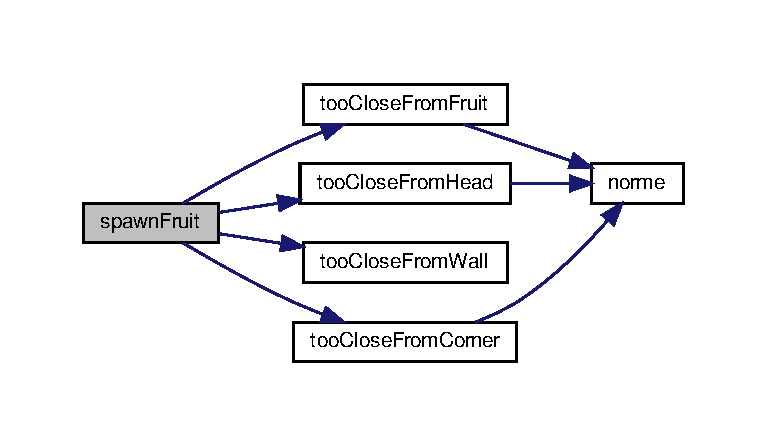
\includegraphics[width=350pt]{snake_8c_a25fd68046ffe688449023d7d4d75c95a_cgraph}
\end{center}
\end{figure}
Voici le graphe des appelants de cette fonction \+:\nopagebreak
\begin{figure}[H]
\begin{center}
\leavevmode
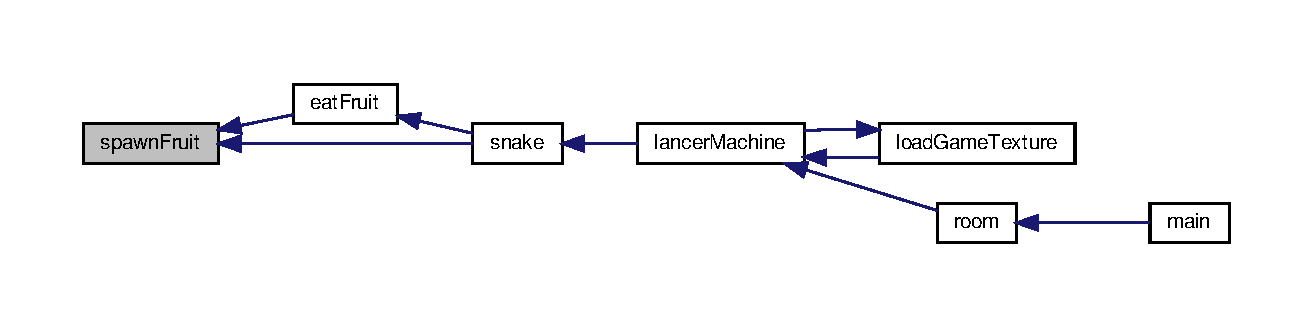
\includegraphics[width=350pt]{snake_8c_a25fd68046ffe688449023d7d4d75c95a_icgraph}
\end{center}
\end{figure}
\mbox{\Hypertarget{snake_8c_a5ab96fad579ff79a2df0bb06e86cb7d0}\label{snake_8c_a5ab96fad579ff79a2df0bb06e86cb7d0}} 
\index{snake.\+c@{snake.\+c}!too\+Close\+From\+Corner@{too\+Close\+From\+Corner}}
\index{too\+Close\+From\+Corner@{too\+Close\+From\+Corner}!snake.\+c@{snake.\+c}}
\subsubsection{\texorpdfstring{too\+Close\+From\+Corner()}{tooCloseFromCorner()}}
{\footnotesize\ttfamily int too\+Close\+From\+Corner (\begin{DoxyParamCaption}\item[{\hyperlink{struct_fruit}{Fruit}}]{fruit }\end{DoxyParamCaption})}



Détermine si un fruit est trop proche d\textquotesingle{}un coin pour pouvoir apparaître. 


\begin{DoxyParams}{Paramètres}
{\em fruit} & Un fruit \\
\hline
\end{DoxyParams}
\begin{DoxyReturn}{Renvoie}
Vrai si il est trop proche, sinon faux 
\end{DoxyReturn}
Voici le graphe d\textquotesingle{}appel pour cette fonction \+:\nopagebreak
\begin{figure}[H]
\begin{center}
\leavevmode
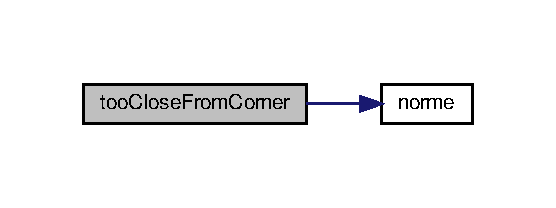
\includegraphics[width=267pt]{snake_8c_a5ab96fad579ff79a2df0bb06e86cb7d0_cgraph}
\end{center}
\end{figure}
Voici le graphe des appelants de cette fonction \+:\nopagebreak
\begin{figure}[H]
\begin{center}
\leavevmode
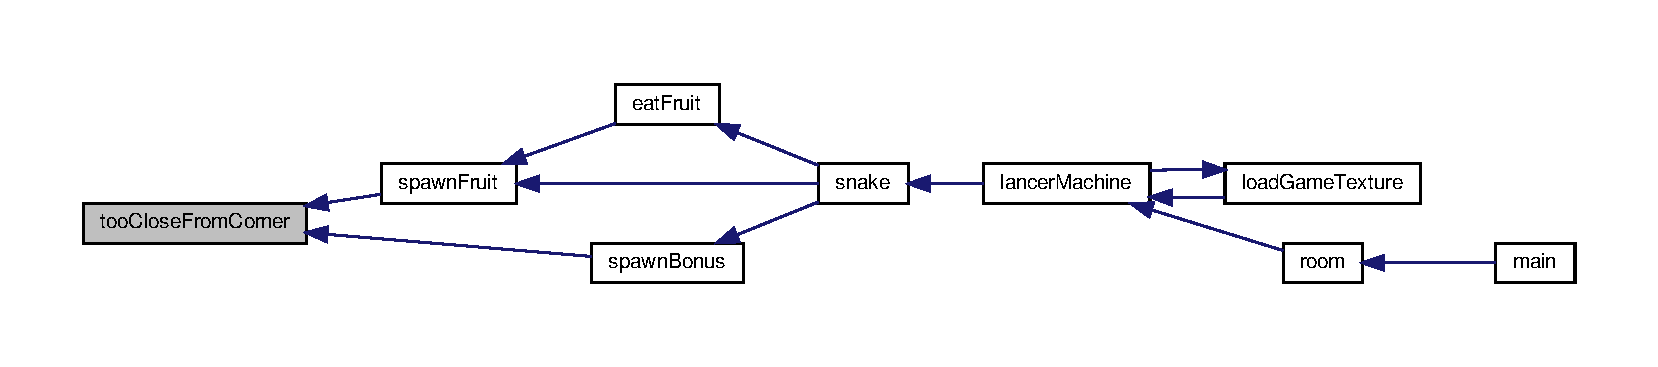
\includegraphics[width=350pt]{snake_8c_a5ab96fad579ff79a2df0bb06e86cb7d0_icgraph}
\end{center}
\end{figure}
\mbox{\Hypertarget{snake_8c_a707860ff76b3c064c97abfb3aa3562d1}\label{snake_8c_a707860ff76b3c064c97abfb3aa3562d1}} 
\index{snake.\+c@{snake.\+c}!too\+Close\+From\+Fruit@{too\+Close\+From\+Fruit}}
\index{too\+Close\+From\+Fruit@{too\+Close\+From\+Fruit}!snake.\+c@{snake.\+c}}
\subsubsection{\texorpdfstring{too\+Close\+From\+Fruit()}{tooCloseFromFruit()}}
{\footnotesize\ttfamily int too\+Close\+From\+Fruit (\begin{DoxyParamCaption}\item[{\hyperlink{struct_fruit}{Fruit} $\ast$}]{fruit\+Rang,  }\item[{int}]{rang,  }\item[{\hyperlink{struct_fruit}{Fruit} $\ast$}]{fruit\+Search,  }\item[{int}]{nb\+Fruit\+Search }\end{DoxyParamCaption})}



Détermine si un fruit est trop d\textquotesingle{}un autre ou d\textquotesingle{}un bonus pour pouvoir apparaître. 


\begin{DoxyParams}{Paramètres}
{\em fruit\+Rang} & Le tableau de fruit \\
\hline
{\em rang} & Le rang du fruit \\
\hline
{\em fruit\+Search} & Le tableau de fruit/bonus où vérifier la proximité \\
\hline
{\em nb\+Fruit\+Search} & Le nombre d\textquotesingle{}élément dans ce tableau \\
\hline
\end{DoxyParams}
\begin{DoxyReturn}{Renvoie}
Vrai si il est trop proche, sinon faux 
\end{DoxyReturn}
Voici le graphe d\textquotesingle{}appel pour cette fonction \+:\nopagebreak
\begin{figure}[H]
\begin{center}
\leavevmode
\includegraphics[width=258pt]{snake_8c_a707860ff76b3c064c97abfb3aa3562d1_cgraph}
\end{center}
\end{figure}
Voici le graphe des appelants de cette fonction \+:\nopagebreak
\begin{figure}[H]
\begin{center}
\leavevmode
\includegraphics[width=350pt]{snake_8c_a707860ff76b3c064c97abfb3aa3562d1_icgraph}
\end{center}
\end{figure}
\mbox{\Hypertarget{snake_8c_aa9234d8c6419bdecdd99e4e9596fdbde}\label{snake_8c_aa9234d8c6419bdecdd99e4e9596fdbde}} 
\index{snake.\+c@{snake.\+c}!too\+Close\+From\+Head@{too\+Close\+From\+Head}}
\index{too\+Close\+From\+Head@{too\+Close\+From\+Head}!snake.\+c@{snake.\+c}}
\subsubsection{\texorpdfstring{too\+Close\+From\+Head()}{tooCloseFromHead()}}
{\footnotesize\ttfamily int too\+Close\+From\+Head (\begin{DoxyParamCaption}\item[{\hyperlink{struct_snake_part}{Snake\+Part}}]{head,  }\item[{\hyperlink{struct_fruit}{Fruit}}]{fruit }\end{DoxyParamCaption})}



Détermine si un fruit est trop proche de la tête pour pouvoir apparaître. 


\begin{DoxyParams}{Paramètres}
{\em head} & La tête du serpent \\
\hline
{\em fruit} & Un fruit \\
\hline
\end{DoxyParams}
\begin{DoxyReturn}{Renvoie}
Vrai si il est trop proche, sinon faux 
\end{DoxyReturn}
Voici le graphe d\textquotesingle{}appel pour cette fonction \+:\nopagebreak
\begin{figure}[H]
\begin{center}
\leavevmode
\includegraphics[width=261pt]{snake_8c_aa9234d8c6419bdecdd99e4e9596fdbde_cgraph}
\end{center}
\end{figure}
Voici le graphe des appelants de cette fonction \+:\nopagebreak
\begin{figure}[H]
\begin{center}
\leavevmode
\includegraphics[width=350pt]{snake_8c_aa9234d8c6419bdecdd99e4e9596fdbde_icgraph}
\end{center}
\end{figure}
\mbox{\Hypertarget{snake_8c_a88e97e8f14fe02486dcdafa98c1c1da5}\label{snake_8c_a88e97e8f14fe02486dcdafa98c1c1da5}} 
\index{snake.\+c@{snake.\+c}!too\+Close\+From\+Wall@{too\+Close\+From\+Wall}}
\index{too\+Close\+From\+Wall@{too\+Close\+From\+Wall}!snake.\+c@{snake.\+c}}
\subsubsection{\texorpdfstring{too\+Close\+From\+Wall()}{tooCloseFromWall()}}
{\footnotesize\ttfamily static int too\+Close\+From\+Wall (\begin{DoxyParamCaption}\item[{Vector2f}]{fruit,  }\item[{int}]{dist }\end{DoxyParamCaption})\hspace{0.3cm}{\ttfamily [static]}}



Détermine si un point est trop proche d\textquotesingle{}un mur par rapport à une distance donnée. 


\begin{DoxyParams}{Paramètres}
{\em point} & Un point \\
\hline
{\em dist} & La distance maximale autorisée \\
\hline
\end{DoxyParams}
\begin{DoxyReturn}{Renvoie}
Vrai si il est trop proche, sinon faux 
\end{DoxyReturn}
Voici le graphe des appelants de cette fonction \+:\nopagebreak
\begin{figure}[H]
\begin{center}
\leavevmode
\includegraphics[width=350pt]{snake_8c_a88e97e8f14fe02486dcdafa98c1c1da5_icgraph}
\end{center}
\end{figure}
\mbox{\Hypertarget{snake_8c_a739086fd85b17cc39593a193118b0682}\label{snake_8c_a739086fd85b17cc39593a193118b0682}} 
\index{snake.\+c@{snake.\+c}!turn\+Left@{turn\+Left}}
\index{turn\+Left@{turn\+Left}!snake.\+c@{snake.\+c}}
\subsubsection{\texorpdfstring{turn\+Left()}{turnLeft()}}
{\footnotesize\ttfamily void turn\+Left (\begin{DoxyParamCaption}\item[{double $\ast$}]{angle }\end{DoxyParamCaption})}



Tourne le serpent vers la gauche. 


\begin{DoxyParams}{Paramètres}
{\em angle} & La direction du serpent \\
\hline
\end{DoxyParams}
Voici le graphe des appelants de cette fonction \+:\nopagebreak
\begin{figure}[H]
\begin{center}
\leavevmode
\includegraphics[width=350pt]{snake_8c_a739086fd85b17cc39593a193118b0682_icgraph}
\end{center}
\end{figure}
\mbox{\Hypertarget{snake_8c_ae92e302f554e9e33c5a52e6251106a89}\label{snake_8c_ae92e302f554e9e33c5a52e6251106a89}} 
\index{snake.\+c@{snake.\+c}!turn\+Right@{turn\+Right}}
\index{turn\+Right@{turn\+Right}!snake.\+c@{snake.\+c}}
\subsubsection{\texorpdfstring{turn\+Right()}{turnRight()}}
{\footnotesize\ttfamily void turn\+Right (\begin{DoxyParamCaption}\item[{double $\ast$}]{angle }\end{DoxyParamCaption})}



Tourne le serpent vers la droite. 


\begin{DoxyParams}{Paramètres}
{\em angle} & La direction du serpent \\
\hline
\end{DoxyParams}
Voici le graphe des appelants de cette fonction \+:\nopagebreak
\begin{figure}[H]
\begin{center}
\leavevmode
\includegraphics[width=350pt]{snake_8c_ae92e302f554e9e33c5a52e6251106a89_icgraph}
\end{center}
\end{figure}


\subsection{Documentation des variables}
\mbox{\Hypertarget{snake_8c_a30862aa51c2944f287c4445751341ee8}\label{snake_8c_a30862aa51c2944f287c4445751341ee8}} 
\index{snake.\+c@{snake.\+c}!update\+Ended@{update\+Ended}}
\index{update\+Ended@{update\+Ended}!snake.\+c@{snake.\+c}}
\subsubsection{\texorpdfstring{update\+Ended}{updateEnded}}
{\footnotesize\ttfamily int update\+Ended}


\hypertarget{flappy__bird_8c}{}\section{Référence du fichier games/3\+\_\+flappy\+\_\+bird/flappy\+\_\+bird.c}
\label{flappy__bird_8c}\index{games/3\+\_\+flappy\+\_\+bird/flappy\+\_\+bird.\+c@{games/3\+\_\+flappy\+\_\+bird/flappy\+\_\+bird.\+c}}


Jeu flappy bird.  


{\ttfamily \#include $<$stdio.\+h$>$}\newline
{\ttfamily \#include $<$time.\+h$>$}\newline
{\ttfamily \#include $<$math.\+h$>$}\newline
{\ttfamily \#include $<$S\+D\+L2/\+S\+D\+L.\+h$>$}\newline
{\ttfamily \#include $<$S\+D\+L2/\+S\+D\+L\+\_\+image.\+h$>$}\newline
{\ttfamily \#include $<$S\+D\+L2/\+S\+D\+L\+\_\+mixer.\+h$>$}\newline
{\ttfamily \#include \char`\"{}../../include/commun\+Functions.\+h\char`\"{}}\newline
{\ttfamily \#include \char`\"{}../../include/lib\+Web.\+h\char`\"{}}\newline
{\ttfamily \#include \char`\"{}../../include/hashage.\+h\char`\"{}}\newline
{\ttfamily \#include \char`\"{}../../include/define.\+h\char`\"{}}\newline
Graphe des dépendances par inclusion de flappy\+\_\+bird.\+c\+:\nopagebreak
\begin{figure}[H]
\begin{center}
\leavevmode
\includegraphics[width=350pt]{flappy__bird_8c__incl}
\end{center}
\end{figure}
\subsection*{Structures de données}
\begin{DoxyCompactItemize}
\item 
struct \hyperlink{structpilonne}{pilonne}
\begin{DoxyCompactList}\small\item\em Stock la position d\textquotesingle{}un obstacle. \end{DoxyCompactList}\end{DoxyCompactItemize}
\subsection*{Macros}
\begin{DoxyCompactItemize}
\item 
\#define \hyperlink{flappy__bird_8c_ae0ceb0aa3313530aa5d72827ea1131c3}{W\+I\+N\+D\+O\+W\+\_\+L}~1920.
\item 
\#define \hyperlink{flappy__bird_8c_ac99e9b1c151b601470732c2c9ff9866f}{W\+I\+N\+D\+O\+W\+\_\+H}~1080.
\item 
\#define \hyperlink{flappy__bird_8c_ac92ca5ab87034a348decad7ee8d4bd1b}{F\+PS}~60
\item 
\#define \hyperlink{flappy__bird_8c_a4330090b097ea40d0041592c7c29fae7}{S\+C\+A\+L\+E\+\_\+\+T\+O\+\_\+\+F\+IT}~4
\item 
\#define \hyperlink{flappy__bird_8c_ac8a6f389427352d1e43f3e5909d7a8a8}{C\+O\+M\+P\+E\+N\+S\+A\+T\+I\+T\+I\+O\+N\+\_\+\+H\+I\+T\+B\+O\+X\+\_\+\+D\+O\+WN}~20
\item 
\#define \hyperlink{flappy__bird_8c_aad789c6c6cd9f5fb4148ee747630f2cc}{P\+R\+E\+L\+O\+A\+D\+\_\+\+P\+O\+S\+\_\+\+O\+B\+S\+T\+A\+C\+LE}~8
\item 
\#define \hyperlink{flappy__bird_8c_aec5e90c4c52efaf97874201e4bbb5a64}{N\+B\+\_\+\+P\+O\+S\+\_\+\+O\+B\+S\+T\+A\+C\+LE}~5
\item 
\#define \hyperlink{flappy__bird_8c_a5455cd891524aaefc0c4b03ceaaaeffa}{T\+R\+A\+N\+C\+H\+E\+\_\+\+P\+O\+S\+\_\+\+O\+B\+S\+T\+A\+C\+LE}~550
\item 
\#define \hyperlink{flappy__bird_8c_adda7fd42446641547476db3522b55a30}{U\+P\+P\+E\+R\+\_\+\+B\+Y\+\_\+\+S\+T\+EP}~30
\item 
\#define \hyperlink{flappy__bird_8c_ad81a2ab0303b14b1f6c567d6219c2d86}{A\+N\+G\+L\+E\+\_\+\+UP}~-\/30
\item 
\#define \hyperlink{flappy__bird_8c_a41081590f4c5b807082e9f7785d1eef9}{A\+N\+G\+L\+E\+\_\+\+D\+O\+WN}~90
\item 
\#define \hyperlink{flappy__bird_8c_ad77f4a1540f49629e52fe9ced51f8f6a}{A\+N\+G\+L\+E\+\_\+\+V\+I\+T\+E\+S\+SE}~8
\item 
\#define \hyperlink{flappy__bird_8c_a1cbcd5e1e513dba8fad4dde27417e221}{B\+A\+N\+\_\+\+C\+O\+DE}~123
\item 
\#define \hyperlink{flappy__bird_8c_ad4b85959fbfc73696e7f51a10c1ffcf3}{D\+I\+R\+\_\+\+F\+L\+A\+P\+\_\+\+W\+AV}~\char`\"{}../games/3\+\_\+flappy\+\_\+bird/\+Sounds/flap.\+wav\char`\"{}
\item 
\#define \hyperlink{flappy__bird_8c_a3d549bcf10a7f1847adae7ba3e71c1cc}{D\+I\+R\+\_\+\+H\+U\+R\+T\+\_\+\+W\+AV}~\char`\"{}../games/3\+\_\+flappy\+\_\+bird/\+Sounds/hurt.\+wav\char`\"{}
\item 
\#define \hyperlink{flappy__bird_8c_a92be272566261416972b218c223ceaea}{D\+I\+R\+\_\+\+S\+C\+O\+R\+E\+\_\+\+W\+AV}~\char`\"{}../games/3\+\_\+flappy\+\_\+bird/\+Sounds/score.\+wav\char`\"{}
\item 
\#define \hyperlink{flappy__bird_8c_ae70f8544bb0fda25dce0a93587d5c6c9}{I\+M\+A\+G\+E\+\_\+\+E\+R\+R\+O\+R\+\_\+\+L\+O\+AD}~-\/101
\item 
\#define \hyperlink{flappy__bird_8c_afb7ee9eee30279bf189e9757a1d28351}{S\+O\+U\+N\+D\+\_\+\+E\+R\+R\+O\+R\+\_\+\+L\+O\+AD}~-\/102
\item 
\#define \hyperlink{flappy__bird_8c_a253eadb4cc9a2d67e636933c9c5e8719}{S\+D\+L\+\_\+\+R\+E\+N\+D\+E\+R\+\_\+\+E\+R\+R\+O\+R\+\_\+\+B\+A\+C\+K\+G\+R\+O\+U\+ND}~-\/103
\item 
\#define \hyperlink{flappy__bird_8c_af33ac46adb014f8b74ad790e8bbb36f8}{S\+D\+L\+\_\+\+R\+E\+N\+D\+E\+R\+\_\+\+E\+R\+R\+O\+R\+\_\+\+O\+B\+S\+T\+A\+C\+LE}~-\/104
\item 
\#define \hyperlink{flappy__bird_8c_a0185ee5ddd06587fcc0e9d2b47773308}{S\+D\+L\+\_\+\+R\+E\+N\+D\+E\+R\+\_\+\+E\+R\+R\+O\+R\+\_\+\+S\+OL}~-\/105
\item 
\#define \hyperlink{flappy__bird_8c_a181905e89f47f1ae6874c5eb19d54fb6}{S\+D\+L\+\_\+\+R\+E\+N\+D\+E\+R\+\_\+\+E\+R\+R\+O\+R\+\_\+\+P\+E\+R\+S\+O\+N\+N\+A\+GE}~-\/106
\item 
\#define \hyperlink{flappy__bird_8c_af4759c7c994c2126f49b584892178831}{S\+D\+L\+\_\+\+R\+E\+N\+D\+E\+R\+\_\+\+E\+R\+R\+O\+R\+\_\+\+P\+R\+I\+N\+T\+\_\+\+S\+C\+O\+RE}~-\/107
\item 
\#define \hyperlink{flappy__bird_8c_af0547979266df72eec654c5552348319}{S\+D\+L\+\_\+\+R\+E\+N\+D\+E\+R\+\_\+\+E\+R\+R\+O\+R\+\_\+\+P\+R\+I\+N\+T\+\_\+\+HS}~-\/108
\end{DoxyCompactItemize}
\subsection*{Fonctions}
\begin{DoxyCompactItemize}
\item 
static int \hyperlink{flappy__bird_8c_a992ce3eab3b684a62428aff5a93ff1f8}{afficher\+Background} (S\+D\+L\+\_\+\+Renderer $\ast$renderer, S\+D\+L\+\_\+\+Texture $\ast$texture\+\_\+background, int theme)
\begin{DoxyCompactList}\small\item\em affiche l\textquotesingle{}image de fond \end{DoxyCompactList}\item 
static int \hyperlink{flappy__bird_8c_ab428543af2e71cb1991d2d037299fbcd}{afficher\+Pilonne} (S\+D\+L\+\_\+\+Renderer $\ast$renderer, S\+D\+L\+\_\+\+Texture $\ast$texture\+\_\+pipes, int position, int position\+\_\+axe\+\_\+x, int theme)
\begin{DoxyCompactList}\small\item\em affiche le O\+B\+S\+T\+A\+C\+LE \end{DoxyCompactList}\item 
static int \hyperlink{flappy__bird_8c_ad4157024daf3d9d27be448ccea30dda9}{afficher\+Sol} (S\+D\+L\+\_\+\+Renderer $\ast$renderer, S\+D\+L\+\_\+\+Texture $\ast$texture\+\_\+sol, int target\+\_\+x)
\begin{DoxyCompactList}\small\item\em affiche le S\+OL D\+E\+C\+O\+RE \end{DoxyCompactList}\item 
static int \hyperlink{flappy__bird_8c_a502412a10243d68aa0dcbd8e07e6edb2}{Afficher\+Personnage} (S\+D\+L\+\_\+\+Renderer $\ast$renderer, S\+D\+L\+\_\+\+Texture $\ast$texture\+\_\+birds, S\+D\+L\+\_\+\+Point emplacement\+Personnage, int var\+Animation\+Personnage, double angle, int theme)
\begin{DoxyCompactList}\small\item\em affiche le personnage a l ecran \end{DoxyCompactList}\item 
static int \hyperlink{flappy__bird_8c_ae61d8a4fce3f39ca4484ea102ea242c1}{int\+Len} (int score)
\begin{DoxyCompactList}\small\item\em retourne la longueur d\textquotesingle{}un nombre \end{DoxyCompactList}\item 
static int \hyperlink{flappy__bird_8c_a49aafde64b048663c89457ab94171d3e}{afficher\+Score} (S\+D\+L\+\_\+\+Renderer $\ast$renderer, S\+D\+L\+\_\+\+Texture $\ast$texture\+\_\+chiffre, int score, int mode)
\begin{DoxyCompactList}\small\item\em affiche le score en cours a l ecran \end{DoxyCompactList}\item 
static int \hyperlink{flappy__bird_8c_a470895aeba5741bc6e77bb164d42e836}{afficher\+Meilleur\+Score} (S\+D\+L\+\_\+\+Renderer $\ast$renderer, S\+D\+L\+\_\+\+Texture $\ast$texture\+\_\+highscore, int score, int high\+\_\+score, int cible)
\begin{DoxyCompactList}\small\item\em affiche le meilleur score a l\textquotesingle{}ecran \end{DoxyCompactList}\item 
static int \hyperlink{flappy__bird_8c_a4858bca7396db08c9733a691a7d58f9c}{afficher\+Tout} (S\+D\+L\+\_\+\+Renderer $\ast$renderer, S\+D\+L\+\_\+\+Thread $\ast$$\ast$\hyperlink{main_8c_a584962a25015c7d6e18e294f55a8bc2d}{thread}, T\+T\+F\+\_\+\+Font $\ast$my\+Font, int $\ast$retour, int $\ast$frame\+\_\+anim\+\_\+loading, int $\ast$frame\+Retour, S\+D\+L\+\_\+\+Texture $\ast$texture\+\_\+loading, S\+D\+L\+\_\+\+Point emplacement\+Personnage, \hyperlink{structpilonne}{pilonne} $\ast$\hyperlink{structpilonne}{pilonne}, int score, int var\+Animation\+Personnage, int var\+Animation\+Sol, int cible, double angle, S\+D\+L\+\_\+\+Texture $\ast$texture\+\_\+background, S\+D\+L\+\_\+\+Texture $\ast$texture\+\_\+pipes, S\+D\+L\+\_\+\+Texture $\ast$texture\+\_\+birds, S\+D\+L\+\_\+\+Texture $\ast$texture\+\_\+medals, S\+D\+L\+\_\+\+Texture $\ast$texture\+\_\+score\+Board, S\+D\+L\+\_\+\+Texture $\ast$texture\+\_\+sol, S\+D\+L\+\_\+\+Texture $\ast$texture\+\_\+chiffre, S\+D\+L\+\_\+\+Texture $\ast$texture\+\_\+highscore, int theme)
\begin{DoxyCompactList}\small\item\em regroupement de toute les fonctions d\textquotesingle{}affichage pour afficher tous \end{DoxyCompactList}\item 
static void \hyperlink{flappy__bird_8c_a5bc0848bb48b6c9265b8b87c7c09b841}{init\+\_\+pilonne} (\hyperlink{structpilonne}{pilonne} $\ast$\hyperlink{structpilonne}{pilonne}, int $\ast$var\+Animation\+Personnage, int $\ast$var\+Animation\+Sol, int $\ast$end, int $\ast$dead, int $\ast$traitement)
\begin{DoxyCompactList}\small\item\em initialisation des pilonnes et des animation et de certaine variables liee au boucle du jeu \end{DoxyCompactList}\item 
static int \hyperlink{flappy__bird_8c_a18e8671a141af5a89d184dd7dcdacc21}{traitement\+\_\+pilonne} (\hyperlink{structpilonne}{pilonne} $\ast$\hyperlink{structpilonne}{pilonne}, int traitement, int $\ast$score, long long $\ast$score\+\_\+hash, long keys\mbox{[}4\mbox{]}, Mix\+\_\+\+Chunk $\ast$score\+\_\+wav)
\begin{DoxyCompactList}\small\item\em detecte le passage d\textquotesingle{}un pilonne et joue un son \end{DoxyCompactList}\item 
static int \hyperlink{flappy__bird_8c_a8b820c5bc000a7a6b332e6cd9fc810fe}{collision} (\hyperlink{structpilonne}{pilonne} $\ast$\hyperlink{structpilonne}{pilonne}, S\+D\+L\+\_\+\+Point emplacement\+Personnage, Mix\+\_\+\+Chunk $\ast$hurt\+\_\+wav)
\begin{DoxyCompactList}\small\item\em permet de detecter une collision et de jouer un son \end{DoxyCompactList}\item 
static void \hyperlink{flappy__bird_8c_a93a55e5f40971511e088f2e52a654c57}{traitement\+Variable\+Animation} (int $\ast$var\+Animation\+Personnage, int $\ast$var\+Animation\+Sol)
\begin{DoxyCompactList}\small\item\em mise a jours des variables liee a l\textquotesingle{}environement/decor \end{DoxyCompactList}\item 
static int \hyperlink{flappy__bird_8c_a0ceb3de339eddf081185c52d40819193}{attendre\+Avant\+Depart} (Mix\+\_\+\+Chunk $\ast$flap\+\_\+wav, int $\ast$rdy\+To\+Space)
\begin{DoxyCompactList}\small\item\em attend l\textquotesingle{}appui sur espace pour demarrer joue un son \end{DoxyCompactList}\item 
static int \hyperlink{flappy__bird_8c_a96e403e8f6333abe2bee8d0429217c7c}{evenement} (int $\ast$upper, int $\ast$vitesse\+Graviter, int $\ast$nb\+\_\+boucle, Mix\+\_\+\+Chunk $\ast$flap\+\_\+wav, int $\ast$rdy\+To\+Space)
\begin{DoxyCompactList}\small\item\em remet les variables au D\+E\+F\+I\+NE si on appui sur espace \end{DoxyCompactList}\item 
static void \hyperlink{flappy__bird_8c_a09c69a458354e11a45af579085123048}{update\+Variable\+Environement} (S\+D\+L\+\_\+\+Point $\ast$emplacement\+Personnage, int $\ast$upper, double $\ast$angle, int $\ast$nb\+\_\+boucle, int $\ast$vitesse\+Graviter)
\begin{DoxyCompactList}\small\item\em permet de mettre a jours les variables utilisez \end{DoxyCompactList}\item 
int \hyperlink{flappy__bird_8c_a8f9872781c9ba0176a187193e39dde97}{flappy\+\_\+bird} (S\+D\+L\+\_\+\+Renderer $\ast$renderer, int highscore, int send\+\_\+l, int send\+\_\+h, char $\ast$token, int hardcore, S\+D\+L\+\_\+\+Texture $\ast$$\ast$\hyperlink{room_8c_a158b90dfedb211efa4c317267c983dd2}{textures})
\begin{DoxyCompactList}\small\item\em Fonction principale qui joue le jeu flappy bird. \end{DoxyCompactList}\end{DoxyCompactItemize}
\subsection*{Variables}
\begin{DoxyCompactItemize}
\item 
const int \hyperlink{flappy__bird_8c_a1563e736047cb57052434e132e4afac4}{F\+R\+A\+M\+E\+\_\+\+T\+I\+ME} = 1000/\hyperlink{flappy__bird_8c_ac92ca5ab87034a348decad7ee8d4bd1b}{F\+PS}
\item 
const S\+D\+L\+\_\+\+Rect \hyperlink{flappy__bird_8c_adf971c6127777fea40325a6b3ccd5179}{B\+A\+C\+K\+G\+R\+O\+U\+ND} = \{0, 0, 144, 256\}
\item 
const S\+D\+L\+\_\+\+Rect \hyperlink{flappy__bird_8c_a871a57bee941abea2174acde4386b3e0}{O\+B\+S\+T\+A\+C\+L\+E\+\_\+\+V\+E\+RT} = \{52,0, 26, 160\}
\item 
const S\+D\+L\+\_\+\+Rect \hyperlink{flappy__bird_8c_adbe7e4a5519e1ca76121ceecaf05c984}{O\+B\+S\+T\+A\+C\+L\+E\+\_\+\+O\+R\+A\+N\+GE} = \{0,0, 26, 160\}
\item 
const S\+D\+L\+\_\+\+Rect \hyperlink{flappy__bird_8c_a086dc677d12a2ef003b8642fd875b470}{S\+OL} = \{0, 0, 168, 55\}
\item 
const S\+D\+L\+\_\+\+Rect \hyperlink{flappy__bird_8c_ae4eeb02b43aebb10a51d6d398895765e}{C\+H\+I\+F\+F\+RE} = \{0, 0, 12, 18\}
\item 
const S\+D\+L\+\_\+\+Rect \hyperlink{flappy__bird_8c_a7aa8f58e4691e6534d4ccae36b92e3e2}{P\+E\+R\+SO} = \{0, 0, 17, 12\}
\item 
const S\+D\+L\+\_\+\+Rect \hyperlink{flappy__bird_8c_a0d4958bc82151e228ae23dc448e879f2}{H\+I\+G\+H\+\_\+\+S\+C\+O\+RE} = \{0,0,512,512\}
\item 
const S\+D\+L\+\_\+\+Rect \hyperlink{flappy__bird_8c_a0e174c1b4b8f590a0ea2051e4918c2fe}{S\+C\+O\+R\+E\+B\+O\+A\+RD} = \{0,0,113,57\}
\item 
const S\+D\+L\+\_\+\+Rect \hyperlink{flappy__bird_8c_ab61fc499948fb2c97e86302b86fa07de}{M\+E\+D\+A\+LS} = \{0,0,22,22\}
\item 
const S\+D\+L\+\_\+\+Color \hyperlink{flappy__bird_8c_a093b04abda57654be8b6ece6e07ab06d}{C\+O\+L\+O\+R\+\_\+\+L\+O\+A\+D\+I\+NG} = \{0x22,0xf4,0x57\}
\item 
int \hyperlink{flappy__bird_8c_a3365e2a32bed45d73157a35657807826}{D\+I\+S\+T\+A\+N\+C\+E\+\_\+\+B\+E\+T\+W\+E\+E\+N\+\_\+\+O\+B\+S\+T\+A\+C\+LE} = 49
\item 
int \hyperlink{flappy__bird_8c_aefe71bca4c41eceec6c77b8d9addfb65}{D\+I\+S\+T\+A\+N\+C\+E\+\_\+\+U\+N\+D\+E\+R\+\_\+\+O\+B\+S\+T\+A\+C\+LE} = 100
\item 
const int \hyperlink{flappy__bird_8c_a676a51616828adeeea54883648de061b}{U\+P\+P\+E\+R\+\_\+\+S\+T\+EP} = 4 $\ast$ (\hyperlink{flappy__bird_8c_ac92ca5ab87034a348decad7ee8d4bd1b}{F\+PS}/30)
\item 
const int \hyperlink{flappy__bird_8c_a5c07d7d9d0c384ff87214edb5f44765b}{G\+R\+A\+V\+I\+T\+Y\+\_\+\+S\+P\+E\+ED} = 2 $\ast$ (\hyperlink{flappy__bird_8c_ac92ca5ab87034a348decad7ee8d4bd1b}{F\+PS}/30)
\item 
const int \hyperlink{flappy__bird_8c_a6d29d77d4db16afe3012ee7ab51f6878}{V\+I\+T\+E\+S\+S\+E\+\_\+\+D\+E\+P\+L\+A\+C\+E\+M\+E\+N\+T\+\_\+\+D\+E\+C\+OR} = 8 / (\hyperlink{flappy__bird_8c_ac92ca5ab87034a348decad7ee8d4bd1b}{F\+PS}/30)
\item 
int \hyperlink{flappy__bird_8c_a30862aa51c2944f287c4445751341ee8}{update\+Ended}
\end{DoxyCompactItemize}


\subsection{Description détaillée}
Jeu flappy bird. 

\begin{DoxyAuthor}{Auteur}
S.\+Mahi 
\end{DoxyAuthor}
\begin{DoxyVersion}{Version}
1.\+0 
\end{DoxyVersion}
\begin{DoxyDate}{Date}
10/01/2020 
\end{DoxyDate}


\subsection{Documentation des macros}
\mbox{\Hypertarget{flappy__bird_8c_a41081590f4c5b807082e9f7785d1eef9}\label{flappy__bird_8c_a41081590f4c5b807082e9f7785d1eef9}} 
\index{flappy\+\_\+bird.\+c@{flappy\+\_\+bird.\+c}!A\+N\+G\+L\+E\+\_\+\+D\+O\+WN@{A\+N\+G\+L\+E\+\_\+\+D\+O\+WN}}
\index{A\+N\+G\+L\+E\+\_\+\+D\+O\+WN@{A\+N\+G\+L\+E\+\_\+\+D\+O\+WN}!flappy\+\_\+bird.\+c@{flappy\+\_\+bird.\+c}}
\subsubsection{\texorpdfstring{A\+N\+G\+L\+E\+\_\+\+D\+O\+WN}{ANGLE\_DOWN}}
{\footnotesize\ttfamily \#define A\+N\+G\+L\+E\+\_\+\+D\+O\+WN~90}

\mbox{\Hypertarget{flappy__bird_8c_ad81a2ab0303b14b1f6c567d6219c2d86}\label{flappy__bird_8c_ad81a2ab0303b14b1f6c567d6219c2d86}} 
\index{flappy\+\_\+bird.\+c@{flappy\+\_\+bird.\+c}!A\+N\+G\+L\+E\+\_\+\+UP@{A\+N\+G\+L\+E\+\_\+\+UP}}
\index{A\+N\+G\+L\+E\+\_\+\+UP@{A\+N\+G\+L\+E\+\_\+\+UP}!flappy\+\_\+bird.\+c@{flappy\+\_\+bird.\+c}}
\subsubsection{\texorpdfstring{A\+N\+G\+L\+E\+\_\+\+UP}{ANGLE\_UP}}
{\footnotesize\ttfamily \#define A\+N\+G\+L\+E\+\_\+\+UP~-\/30}

\mbox{\Hypertarget{flappy__bird_8c_ad77f4a1540f49629e52fe9ced51f8f6a}\label{flappy__bird_8c_ad77f4a1540f49629e52fe9ced51f8f6a}} 
\index{flappy\+\_\+bird.\+c@{flappy\+\_\+bird.\+c}!A\+N\+G\+L\+E\+\_\+\+V\+I\+T\+E\+S\+SE@{A\+N\+G\+L\+E\+\_\+\+V\+I\+T\+E\+S\+SE}}
\index{A\+N\+G\+L\+E\+\_\+\+V\+I\+T\+E\+S\+SE@{A\+N\+G\+L\+E\+\_\+\+V\+I\+T\+E\+S\+SE}!flappy\+\_\+bird.\+c@{flappy\+\_\+bird.\+c}}
\subsubsection{\texorpdfstring{A\+N\+G\+L\+E\+\_\+\+V\+I\+T\+E\+S\+SE}{ANGLE\_VITESSE}}
{\footnotesize\ttfamily \#define A\+N\+G\+L\+E\+\_\+\+V\+I\+T\+E\+S\+SE~8}

\mbox{\Hypertarget{flappy__bird_8c_a1cbcd5e1e513dba8fad4dde27417e221}\label{flappy__bird_8c_a1cbcd5e1e513dba8fad4dde27417e221}} 
\index{flappy\+\_\+bird.\+c@{flappy\+\_\+bird.\+c}!B\+A\+N\+\_\+\+C\+O\+DE@{B\+A\+N\+\_\+\+C\+O\+DE}}
\index{B\+A\+N\+\_\+\+C\+O\+DE@{B\+A\+N\+\_\+\+C\+O\+DE}!flappy\+\_\+bird.\+c@{flappy\+\_\+bird.\+c}}
\subsubsection{\texorpdfstring{B\+A\+N\+\_\+\+C\+O\+DE}{BAN\_CODE}}
{\footnotesize\ttfamily \#define B\+A\+N\+\_\+\+C\+O\+DE~123}

\mbox{\Hypertarget{flappy__bird_8c_ac8a6f389427352d1e43f3e5909d7a8a8}\label{flappy__bird_8c_ac8a6f389427352d1e43f3e5909d7a8a8}} 
\index{flappy\+\_\+bird.\+c@{flappy\+\_\+bird.\+c}!C\+O\+M\+P\+E\+N\+S\+A\+T\+I\+T\+I\+O\+N\+\_\+\+H\+I\+T\+B\+O\+X\+\_\+\+D\+O\+WN@{C\+O\+M\+P\+E\+N\+S\+A\+T\+I\+T\+I\+O\+N\+\_\+\+H\+I\+T\+B\+O\+X\+\_\+\+D\+O\+WN}}
\index{C\+O\+M\+P\+E\+N\+S\+A\+T\+I\+T\+I\+O\+N\+\_\+\+H\+I\+T\+B\+O\+X\+\_\+\+D\+O\+WN@{C\+O\+M\+P\+E\+N\+S\+A\+T\+I\+T\+I\+O\+N\+\_\+\+H\+I\+T\+B\+O\+X\+\_\+\+D\+O\+WN}!flappy\+\_\+bird.\+c@{flappy\+\_\+bird.\+c}}
\subsubsection{\texorpdfstring{C\+O\+M\+P\+E\+N\+S\+A\+T\+I\+T\+I\+O\+N\+\_\+\+H\+I\+T\+B\+O\+X\+\_\+\+D\+O\+WN}{COMPENSATITION\_HITBOX\_DOWN}}
{\footnotesize\ttfamily \#define C\+O\+M\+P\+E\+N\+S\+A\+T\+I\+T\+I\+O\+N\+\_\+\+H\+I\+T\+B\+O\+X\+\_\+\+D\+O\+WN~20}

\mbox{\Hypertarget{flappy__bird_8c_ad4b85959fbfc73696e7f51a10c1ffcf3}\label{flappy__bird_8c_ad4b85959fbfc73696e7f51a10c1ffcf3}} 
\index{flappy\+\_\+bird.\+c@{flappy\+\_\+bird.\+c}!D\+I\+R\+\_\+\+F\+L\+A\+P\+\_\+\+W\+AV@{D\+I\+R\+\_\+\+F\+L\+A\+P\+\_\+\+W\+AV}}
\index{D\+I\+R\+\_\+\+F\+L\+A\+P\+\_\+\+W\+AV@{D\+I\+R\+\_\+\+F\+L\+A\+P\+\_\+\+W\+AV}!flappy\+\_\+bird.\+c@{flappy\+\_\+bird.\+c}}
\subsubsection{\texorpdfstring{D\+I\+R\+\_\+\+F\+L\+A\+P\+\_\+\+W\+AV}{DIR\_FLAP\_WAV}}
{\footnotesize\ttfamily \#define D\+I\+R\+\_\+\+F\+L\+A\+P\+\_\+\+W\+AV~\char`\"{}../games/3\+\_\+flappy\+\_\+bird/\+Sounds/flap.\+wav\char`\"{}}

\mbox{\Hypertarget{flappy__bird_8c_a3d549bcf10a7f1847adae7ba3e71c1cc}\label{flappy__bird_8c_a3d549bcf10a7f1847adae7ba3e71c1cc}} 
\index{flappy\+\_\+bird.\+c@{flappy\+\_\+bird.\+c}!D\+I\+R\+\_\+\+H\+U\+R\+T\+\_\+\+W\+AV@{D\+I\+R\+\_\+\+H\+U\+R\+T\+\_\+\+W\+AV}}
\index{D\+I\+R\+\_\+\+H\+U\+R\+T\+\_\+\+W\+AV@{D\+I\+R\+\_\+\+H\+U\+R\+T\+\_\+\+W\+AV}!flappy\+\_\+bird.\+c@{flappy\+\_\+bird.\+c}}
\subsubsection{\texorpdfstring{D\+I\+R\+\_\+\+H\+U\+R\+T\+\_\+\+W\+AV}{DIR\_HURT\_WAV}}
{\footnotesize\ttfamily \#define D\+I\+R\+\_\+\+H\+U\+R\+T\+\_\+\+W\+AV~\char`\"{}../games/3\+\_\+flappy\+\_\+bird/\+Sounds/hurt.\+wav\char`\"{}}

\mbox{\Hypertarget{flappy__bird_8c_a92be272566261416972b218c223ceaea}\label{flappy__bird_8c_a92be272566261416972b218c223ceaea}} 
\index{flappy\+\_\+bird.\+c@{flappy\+\_\+bird.\+c}!D\+I\+R\+\_\+\+S\+C\+O\+R\+E\+\_\+\+W\+AV@{D\+I\+R\+\_\+\+S\+C\+O\+R\+E\+\_\+\+W\+AV}}
\index{D\+I\+R\+\_\+\+S\+C\+O\+R\+E\+\_\+\+W\+AV@{D\+I\+R\+\_\+\+S\+C\+O\+R\+E\+\_\+\+W\+AV}!flappy\+\_\+bird.\+c@{flappy\+\_\+bird.\+c}}
\subsubsection{\texorpdfstring{D\+I\+R\+\_\+\+S\+C\+O\+R\+E\+\_\+\+W\+AV}{DIR\_SCORE\_WAV}}
{\footnotesize\ttfamily \#define D\+I\+R\+\_\+\+S\+C\+O\+R\+E\+\_\+\+W\+AV~\char`\"{}../games/3\+\_\+flappy\+\_\+bird/\+Sounds/score.\+wav\char`\"{}}

\mbox{\Hypertarget{flappy__bird_8c_ac92ca5ab87034a348decad7ee8d4bd1b}\label{flappy__bird_8c_ac92ca5ab87034a348decad7ee8d4bd1b}} 
\index{flappy\+\_\+bird.\+c@{flappy\+\_\+bird.\+c}!F\+PS@{F\+PS}}
\index{F\+PS@{F\+PS}!flappy\+\_\+bird.\+c@{flappy\+\_\+bird.\+c}}
\subsubsection{\texorpdfstring{F\+PS}{FPS}}
{\footnotesize\ttfamily \#define F\+PS~60}

\mbox{\Hypertarget{flappy__bird_8c_ae70f8544bb0fda25dce0a93587d5c6c9}\label{flappy__bird_8c_ae70f8544bb0fda25dce0a93587d5c6c9}} 
\index{flappy\+\_\+bird.\+c@{flappy\+\_\+bird.\+c}!I\+M\+A\+G\+E\+\_\+\+E\+R\+R\+O\+R\+\_\+\+L\+O\+AD@{I\+M\+A\+G\+E\+\_\+\+E\+R\+R\+O\+R\+\_\+\+L\+O\+AD}}
\index{I\+M\+A\+G\+E\+\_\+\+E\+R\+R\+O\+R\+\_\+\+L\+O\+AD@{I\+M\+A\+G\+E\+\_\+\+E\+R\+R\+O\+R\+\_\+\+L\+O\+AD}!flappy\+\_\+bird.\+c@{flappy\+\_\+bird.\+c}}
\subsubsection{\texorpdfstring{I\+M\+A\+G\+E\+\_\+\+E\+R\+R\+O\+R\+\_\+\+L\+O\+AD}{IMAGE\_ERROR\_LOAD}}
{\footnotesize\ttfamily \#define I\+M\+A\+G\+E\+\_\+\+E\+R\+R\+O\+R\+\_\+\+L\+O\+AD~-\/101}

\mbox{\Hypertarget{flappy__bird_8c_aec5e90c4c52efaf97874201e4bbb5a64}\label{flappy__bird_8c_aec5e90c4c52efaf97874201e4bbb5a64}} 
\index{flappy\+\_\+bird.\+c@{flappy\+\_\+bird.\+c}!N\+B\+\_\+\+P\+O\+S\+\_\+\+O\+B\+S\+T\+A\+C\+LE@{N\+B\+\_\+\+P\+O\+S\+\_\+\+O\+B\+S\+T\+A\+C\+LE}}
\index{N\+B\+\_\+\+P\+O\+S\+\_\+\+O\+B\+S\+T\+A\+C\+LE@{N\+B\+\_\+\+P\+O\+S\+\_\+\+O\+B\+S\+T\+A\+C\+LE}!flappy\+\_\+bird.\+c@{flappy\+\_\+bird.\+c}}
\subsubsection{\texorpdfstring{N\+B\+\_\+\+P\+O\+S\+\_\+\+O\+B\+S\+T\+A\+C\+LE}{NB\_POS\_OBSTACLE}}
{\footnotesize\ttfamily \#define N\+B\+\_\+\+P\+O\+S\+\_\+\+O\+B\+S\+T\+A\+C\+LE~5}

\mbox{\Hypertarget{flappy__bird_8c_aad789c6c6cd9f5fb4148ee747630f2cc}\label{flappy__bird_8c_aad789c6c6cd9f5fb4148ee747630f2cc}} 
\index{flappy\+\_\+bird.\+c@{flappy\+\_\+bird.\+c}!P\+R\+E\+L\+O\+A\+D\+\_\+\+P\+O\+S\+\_\+\+O\+B\+S\+T\+A\+C\+LE@{P\+R\+E\+L\+O\+A\+D\+\_\+\+P\+O\+S\+\_\+\+O\+B\+S\+T\+A\+C\+LE}}
\index{P\+R\+E\+L\+O\+A\+D\+\_\+\+P\+O\+S\+\_\+\+O\+B\+S\+T\+A\+C\+LE@{P\+R\+E\+L\+O\+A\+D\+\_\+\+P\+O\+S\+\_\+\+O\+B\+S\+T\+A\+C\+LE}!flappy\+\_\+bird.\+c@{flappy\+\_\+bird.\+c}}
\subsubsection{\texorpdfstring{P\+R\+E\+L\+O\+A\+D\+\_\+\+P\+O\+S\+\_\+\+O\+B\+S\+T\+A\+C\+LE}{PRELOAD\_POS\_OBSTACLE}}
{\footnotesize\ttfamily \#define P\+R\+E\+L\+O\+A\+D\+\_\+\+P\+O\+S\+\_\+\+O\+B\+S\+T\+A\+C\+LE~8}

\mbox{\Hypertarget{flappy__bird_8c_a4330090b097ea40d0041592c7c29fae7}\label{flappy__bird_8c_a4330090b097ea40d0041592c7c29fae7}} 
\index{flappy\+\_\+bird.\+c@{flappy\+\_\+bird.\+c}!S\+C\+A\+L\+E\+\_\+\+T\+O\+\_\+\+F\+IT@{S\+C\+A\+L\+E\+\_\+\+T\+O\+\_\+\+F\+IT}}
\index{S\+C\+A\+L\+E\+\_\+\+T\+O\+\_\+\+F\+IT@{S\+C\+A\+L\+E\+\_\+\+T\+O\+\_\+\+F\+IT}!flappy\+\_\+bird.\+c@{flappy\+\_\+bird.\+c}}
\subsubsection{\texorpdfstring{S\+C\+A\+L\+E\+\_\+\+T\+O\+\_\+\+F\+IT}{SCALE\_TO\_FIT}}
{\footnotesize\ttfamily \#define S\+C\+A\+L\+E\+\_\+\+T\+O\+\_\+\+F\+IT~4}

\mbox{\Hypertarget{flappy__bird_8c_a253eadb4cc9a2d67e636933c9c5e8719}\label{flappy__bird_8c_a253eadb4cc9a2d67e636933c9c5e8719}} 
\index{flappy\+\_\+bird.\+c@{flappy\+\_\+bird.\+c}!S\+D\+L\+\_\+\+R\+E\+N\+D\+E\+R\+\_\+\+E\+R\+R\+O\+R\+\_\+\+B\+A\+C\+K\+G\+R\+O\+U\+ND@{S\+D\+L\+\_\+\+R\+E\+N\+D\+E\+R\+\_\+\+E\+R\+R\+O\+R\+\_\+\+B\+A\+C\+K\+G\+R\+O\+U\+ND}}
\index{S\+D\+L\+\_\+\+R\+E\+N\+D\+E\+R\+\_\+\+E\+R\+R\+O\+R\+\_\+\+B\+A\+C\+K\+G\+R\+O\+U\+ND@{S\+D\+L\+\_\+\+R\+E\+N\+D\+E\+R\+\_\+\+E\+R\+R\+O\+R\+\_\+\+B\+A\+C\+K\+G\+R\+O\+U\+ND}!flappy\+\_\+bird.\+c@{flappy\+\_\+bird.\+c}}
\subsubsection{\texorpdfstring{S\+D\+L\+\_\+\+R\+E\+N\+D\+E\+R\+\_\+\+E\+R\+R\+O\+R\+\_\+\+B\+A\+C\+K\+G\+R\+O\+U\+ND}{SDL\_RENDER\_ERROR\_BACKGROUND}}
{\footnotesize\ttfamily \#define S\+D\+L\+\_\+\+R\+E\+N\+D\+E\+R\+\_\+\+E\+R\+R\+O\+R\+\_\+\+B\+A\+C\+K\+G\+R\+O\+U\+ND~-\/103}

\mbox{\Hypertarget{flappy__bird_8c_af33ac46adb014f8b74ad790e8bbb36f8}\label{flappy__bird_8c_af33ac46adb014f8b74ad790e8bbb36f8}} 
\index{flappy\+\_\+bird.\+c@{flappy\+\_\+bird.\+c}!S\+D\+L\+\_\+\+R\+E\+N\+D\+E\+R\+\_\+\+E\+R\+R\+O\+R\+\_\+\+O\+B\+S\+T\+A\+C\+LE@{S\+D\+L\+\_\+\+R\+E\+N\+D\+E\+R\+\_\+\+E\+R\+R\+O\+R\+\_\+\+O\+B\+S\+T\+A\+C\+LE}}
\index{S\+D\+L\+\_\+\+R\+E\+N\+D\+E\+R\+\_\+\+E\+R\+R\+O\+R\+\_\+\+O\+B\+S\+T\+A\+C\+LE@{S\+D\+L\+\_\+\+R\+E\+N\+D\+E\+R\+\_\+\+E\+R\+R\+O\+R\+\_\+\+O\+B\+S\+T\+A\+C\+LE}!flappy\+\_\+bird.\+c@{flappy\+\_\+bird.\+c}}
\subsubsection{\texorpdfstring{S\+D\+L\+\_\+\+R\+E\+N\+D\+E\+R\+\_\+\+E\+R\+R\+O\+R\+\_\+\+O\+B\+S\+T\+A\+C\+LE}{SDL\_RENDER\_ERROR\_OBSTACLE}}
{\footnotesize\ttfamily \#define S\+D\+L\+\_\+\+R\+E\+N\+D\+E\+R\+\_\+\+E\+R\+R\+O\+R\+\_\+\+O\+B\+S\+T\+A\+C\+LE~-\/104}

\mbox{\Hypertarget{flappy__bird_8c_a181905e89f47f1ae6874c5eb19d54fb6}\label{flappy__bird_8c_a181905e89f47f1ae6874c5eb19d54fb6}} 
\index{flappy\+\_\+bird.\+c@{flappy\+\_\+bird.\+c}!S\+D\+L\+\_\+\+R\+E\+N\+D\+E\+R\+\_\+\+E\+R\+R\+O\+R\+\_\+\+P\+E\+R\+S\+O\+N\+N\+A\+GE@{S\+D\+L\+\_\+\+R\+E\+N\+D\+E\+R\+\_\+\+E\+R\+R\+O\+R\+\_\+\+P\+E\+R\+S\+O\+N\+N\+A\+GE}}
\index{S\+D\+L\+\_\+\+R\+E\+N\+D\+E\+R\+\_\+\+E\+R\+R\+O\+R\+\_\+\+P\+E\+R\+S\+O\+N\+N\+A\+GE@{S\+D\+L\+\_\+\+R\+E\+N\+D\+E\+R\+\_\+\+E\+R\+R\+O\+R\+\_\+\+P\+E\+R\+S\+O\+N\+N\+A\+GE}!flappy\+\_\+bird.\+c@{flappy\+\_\+bird.\+c}}
\subsubsection{\texorpdfstring{S\+D\+L\+\_\+\+R\+E\+N\+D\+E\+R\+\_\+\+E\+R\+R\+O\+R\+\_\+\+P\+E\+R\+S\+O\+N\+N\+A\+GE}{SDL\_RENDER\_ERROR\_PERSONNAGE}}
{\footnotesize\ttfamily \#define S\+D\+L\+\_\+\+R\+E\+N\+D\+E\+R\+\_\+\+E\+R\+R\+O\+R\+\_\+\+P\+E\+R\+S\+O\+N\+N\+A\+GE~-\/106}

\mbox{\Hypertarget{flappy__bird_8c_af0547979266df72eec654c5552348319}\label{flappy__bird_8c_af0547979266df72eec654c5552348319}} 
\index{flappy\+\_\+bird.\+c@{flappy\+\_\+bird.\+c}!S\+D\+L\+\_\+\+R\+E\+N\+D\+E\+R\+\_\+\+E\+R\+R\+O\+R\+\_\+\+P\+R\+I\+N\+T\+\_\+\+HS@{S\+D\+L\+\_\+\+R\+E\+N\+D\+E\+R\+\_\+\+E\+R\+R\+O\+R\+\_\+\+P\+R\+I\+N\+T\+\_\+\+HS}}
\index{S\+D\+L\+\_\+\+R\+E\+N\+D\+E\+R\+\_\+\+E\+R\+R\+O\+R\+\_\+\+P\+R\+I\+N\+T\+\_\+\+HS@{S\+D\+L\+\_\+\+R\+E\+N\+D\+E\+R\+\_\+\+E\+R\+R\+O\+R\+\_\+\+P\+R\+I\+N\+T\+\_\+\+HS}!flappy\+\_\+bird.\+c@{flappy\+\_\+bird.\+c}}
\subsubsection{\texorpdfstring{S\+D\+L\+\_\+\+R\+E\+N\+D\+E\+R\+\_\+\+E\+R\+R\+O\+R\+\_\+\+P\+R\+I\+N\+T\+\_\+\+HS}{SDL\_RENDER\_ERROR\_PRINT\_HS}}
{\footnotesize\ttfamily \#define S\+D\+L\+\_\+\+R\+E\+N\+D\+E\+R\+\_\+\+E\+R\+R\+O\+R\+\_\+\+P\+R\+I\+N\+T\+\_\+\+HS~-\/108}

\mbox{\Hypertarget{flappy__bird_8c_af4759c7c994c2126f49b584892178831}\label{flappy__bird_8c_af4759c7c994c2126f49b584892178831}} 
\index{flappy\+\_\+bird.\+c@{flappy\+\_\+bird.\+c}!S\+D\+L\+\_\+\+R\+E\+N\+D\+E\+R\+\_\+\+E\+R\+R\+O\+R\+\_\+\+P\+R\+I\+N\+T\+\_\+\+S\+C\+O\+RE@{S\+D\+L\+\_\+\+R\+E\+N\+D\+E\+R\+\_\+\+E\+R\+R\+O\+R\+\_\+\+P\+R\+I\+N\+T\+\_\+\+S\+C\+O\+RE}}
\index{S\+D\+L\+\_\+\+R\+E\+N\+D\+E\+R\+\_\+\+E\+R\+R\+O\+R\+\_\+\+P\+R\+I\+N\+T\+\_\+\+S\+C\+O\+RE@{S\+D\+L\+\_\+\+R\+E\+N\+D\+E\+R\+\_\+\+E\+R\+R\+O\+R\+\_\+\+P\+R\+I\+N\+T\+\_\+\+S\+C\+O\+RE}!flappy\+\_\+bird.\+c@{flappy\+\_\+bird.\+c}}
\subsubsection{\texorpdfstring{S\+D\+L\+\_\+\+R\+E\+N\+D\+E\+R\+\_\+\+E\+R\+R\+O\+R\+\_\+\+P\+R\+I\+N\+T\+\_\+\+S\+C\+O\+RE}{SDL\_RENDER\_ERROR\_PRINT\_SCORE}}
{\footnotesize\ttfamily \#define S\+D\+L\+\_\+\+R\+E\+N\+D\+E\+R\+\_\+\+E\+R\+R\+O\+R\+\_\+\+P\+R\+I\+N\+T\+\_\+\+S\+C\+O\+RE~-\/107}

\mbox{\Hypertarget{flappy__bird_8c_a0185ee5ddd06587fcc0e9d2b47773308}\label{flappy__bird_8c_a0185ee5ddd06587fcc0e9d2b47773308}} 
\index{flappy\+\_\+bird.\+c@{flappy\+\_\+bird.\+c}!S\+D\+L\+\_\+\+R\+E\+N\+D\+E\+R\+\_\+\+E\+R\+R\+O\+R\+\_\+\+S\+OL@{S\+D\+L\+\_\+\+R\+E\+N\+D\+E\+R\+\_\+\+E\+R\+R\+O\+R\+\_\+\+S\+OL}}
\index{S\+D\+L\+\_\+\+R\+E\+N\+D\+E\+R\+\_\+\+E\+R\+R\+O\+R\+\_\+\+S\+OL@{S\+D\+L\+\_\+\+R\+E\+N\+D\+E\+R\+\_\+\+E\+R\+R\+O\+R\+\_\+\+S\+OL}!flappy\+\_\+bird.\+c@{flappy\+\_\+bird.\+c}}
\subsubsection{\texorpdfstring{S\+D\+L\+\_\+\+R\+E\+N\+D\+E\+R\+\_\+\+E\+R\+R\+O\+R\+\_\+\+S\+OL}{SDL\_RENDER\_ERROR\_SOL}}
{\footnotesize\ttfamily \#define S\+D\+L\+\_\+\+R\+E\+N\+D\+E\+R\+\_\+\+E\+R\+R\+O\+R\+\_\+\+S\+OL~-\/105}

\mbox{\Hypertarget{flappy__bird_8c_afb7ee9eee30279bf189e9757a1d28351}\label{flappy__bird_8c_afb7ee9eee30279bf189e9757a1d28351}} 
\index{flappy\+\_\+bird.\+c@{flappy\+\_\+bird.\+c}!S\+O\+U\+N\+D\+\_\+\+E\+R\+R\+O\+R\+\_\+\+L\+O\+AD@{S\+O\+U\+N\+D\+\_\+\+E\+R\+R\+O\+R\+\_\+\+L\+O\+AD}}
\index{S\+O\+U\+N\+D\+\_\+\+E\+R\+R\+O\+R\+\_\+\+L\+O\+AD@{S\+O\+U\+N\+D\+\_\+\+E\+R\+R\+O\+R\+\_\+\+L\+O\+AD}!flappy\+\_\+bird.\+c@{flappy\+\_\+bird.\+c}}
\subsubsection{\texorpdfstring{S\+O\+U\+N\+D\+\_\+\+E\+R\+R\+O\+R\+\_\+\+L\+O\+AD}{SOUND\_ERROR\_LOAD}}
{\footnotesize\ttfamily \#define S\+O\+U\+N\+D\+\_\+\+E\+R\+R\+O\+R\+\_\+\+L\+O\+AD~-\/102}

\mbox{\Hypertarget{flappy__bird_8c_a5455cd891524aaefc0c4b03ceaaaeffa}\label{flappy__bird_8c_a5455cd891524aaefc0c4b03ceaaaeffa}} 
\index{flappy\+\_\+bird.\+c@{flappy\+\_\+bird.\+c}!T\+R\+A\+N\+C\+H\+E\+\_\+\+P\+O\+S\+\_\+\+O\+B\+S\+T\+A\+C\+LE@{T\+R\+A\+N\+C\+H\+E\+\_\+\+P\+O\+S\+\_\+\+O\+B\+S\+T\+A\+C\+LE}}
\index{T\+R\+A\+N\+C\+H\+E\+\_\+\+P\+O\+S\+\_\+\+O\+B\+S\+T\+A\+C\+LE@{T\+R\+A\+N\+C\+H\+E\+\_\+\+P\+O\+S\+\_\+\+O\+B\+S\+T\+A\+C\+LE}!flappy\+\_\+bird.\+c@{flappy\+\_\+bird.\+c}}
\subsubsection{\texorpdfstring{T\+R\+A\+N\+C\+H\+E\+\_\+\+P\+O\+S\+\_\+\+O\+B\+S\+T\+A\+C\+LE}{TRANCHE\_POS\_OBSTACLE}}
{\footnotesize\ttfamily \#define T\+R\+A\+N\+C\+H\+E\+\_\+\+P\+O\+S\+\_\+\+O\+B\+S\+T\+A\+C\+LE~550}

\mbox{\Hypertarget{flappy__bird_8c_adda7fd42446641547476db3522b55a30}\label{flappy__bird_8c_adda7fd42446641547476db3522b55a30}} 
\index{flappy\+\_\+bird.\+c@{flappy\+\_\+bird.\+c}!U\+P\+P\+E\+R\+\_\+\+B\+Y\+\_\+\+S\+T\+EP@{U\+P\+P\+E\+R\+\_\+\+B\+Y\+\_\+\+S\+T\+EP}}
\index{U\+P\+P\+E\+R\+\_\+\+B\+Y\+\_\+\+S\+T\+EP@{U\+P\+P\+E\+R\+\_\+\+B\+Y\+\_\+\+S\+T\+EP}!flappy\+\_\+bird.\+c@{flappy\+\_\+bird.\+c}}
\subsubsection{\texorpdfstring{U\+P\+P\+E\+R\+\_\+\+B\+Y\+\_\+\+S\+T\+EP}{UPPER\_BY\_STEP}}
{\footnotesize\ttfamily \#define U\+P\+P\+E\+R\+\_\+\+B\+Y\+\_\+\+S\+T\+EP~30}

\mbox{\Hypertarget{flappy__bird_8c_ac99e9b1c151b601470732c2c9ff9866f}\label{flappy__bird_8c_ac99e9b1c151b601470732c2c9ff9866f}} 
\index{flappy\+\_\+bird.\+c@{flappy\+\_\+bird.\+c}!W\+I\+N\+D\+O\+W\+\_\+H@{W\+I\+N\+D\+O\+W\+\_\+H}}
\index{W\+I\+N\+D\+O\+W\+\_\+H@{W\+I\+N\+D\+O\+W\+\_\+H}!flappy\+\_\+bird.\+c@{flappy\+\_\+bird.\+c}}
\subsubsection{\texorpdfstring{W\+I\+N\+D\+O\+W\+\_\+H}{WINDOW\_H}}
{\footnotesize\ttfamily \#define W\+I\+N\+D\+O\+W\+\_\+H~1080.}

\mbox{\Hypertarget{flappy__bird_8c_ae0ceb0aa3313530aa5d72827ea1131c3}\label{flappy__bird_8c_ae0ceb0aa3313530aa5d72827ea1131c3}} 
\index{flappy\+\_\+bird.\+c@{flappy\+\_\+bird.\+c}!W\+I\+N\+D\+O\+W\+\_\+L@{W\+I\+N\+D\+O\+W\+\_\+L}}
\index{W\+I\+N\+D\+O\+W\+\_\+L@{W\+I\+N\+D\+O\+W\+\_\+L}!flappy\+\_\+bird.\+c@{flappy\+\_\+bird.\+c}}
\subsubsection{\texorpdfstring{W\+I\+N\+D\+O\+W\+\_\+L}{WINDOW\_L}}
{\footnotesize\ttfamily \#define W\+I\+N\+D\+O\+W\+\_\+L~1920.}



\subsection{Documentation des fonctions}
\mbox{\Hypertarget{flappy__bird_8c_a992ce3eab3b684a62428aff5a93ff1f8}\label{flappy__bird_8c_a992ce3eab3b684a62428aff5a93ff1f8}} 
\index{flappy\+\_\+bird.\+c@{flappy\+\_\+bird.\+c}!afficher\+Background@{afficher\+Background}}
\index{afficher\+Background@{afficher\+Background}!flappy\+\_\+bird.\+c@{flappy\+\_\+bird.\+c}}
\subsubsection{\texorpdfstring{afficher\+Background()}{afficherBackground()}}
{\footnotesize\ttfamily int afficher\+Background (\begin{DoxyParamCaption}\item[{S\+D\+L\+\_\+\+Renderer $\ast$}]{renderer,  }\item[{S\+D\+L\+\_\+\+Texture $\ast$}]{texture\+\_\+background,  }\item[{int}]{theme }\end{DoxyParamCaption})\hspace{0.3cm}{\ttfamily [static]}}



affiche l\textquotesingle{}image de fond 


\begin{DoxyParams}{Paramètres}
{\em renderer} & \\
\hline
{\em texture\+\_\+background} & \\
\hline
{\em theme} & \\
\hline
\end{DoxyParams}
\begin{DoxyReturn}{Renvoie}
E\+X\+I\+T\+\_\+\+S\+U\+C\+C\+E\+SS / E\+X\+I\+T\+\_\+\+F\+A\+I\+L\+U\+RE 
\end{DoxyReturn}
Voici le graphe des appelants de cette fonction \+:\nopagebreak
\begin{figure}[H]
\begin{center}
\leavevmode
\includegraphics[width=350pt]{flappy__bird_8c_a992ce3eab3b684a62428aff5a93ff1f8_icgraph}
\end{center}
\end{figure}
\mbox{\Hypertarget{flappy__bird_8c_a470895aeba5741bc6e77bb164d42e836}\label{flappy__bird_8c_a470895aeba5741bc6e77bb164d42e836}} 
\index{flappy\+\_\+bird.\+c@{flappy\+\_\+bird.\+c}!afficher\+Meilleur\+Score@{afficher\+Meilleur\+Score}}
\index{afficher\+Meilleur\+Score@{afficher\+Meilleur\+Score}!flappy\+\_\+bird.\+c@{flappy\+\_\+bird.\+c}}
\subsubsection{\texorpdfstring{afficher\+Meilleur\+Score()}{afficherMeilleurScore()}}
{\footnotesize\ttfamily int afficher\+Meilleur\+Score (\begin{DoxyParamCaption}\item[{S\+D\+L\+\_\+\+Renderer $\ast$}]{renderer,  }\item[{S\+D\+L\+\_\+\+Texture $\ast$}]{texture\+\_\+highscore,  }\item[{int}]{score,  }\item[{int}]{high\+\_\+score,  }\item[{int}]{cible }\end{DoxyParamCaption})\hspace{0.3cm}{\ttfamily [static]}}



affiche le meilleur score a l\textquotesingle{}ecran 


\begin{DoxyParams}{Paramètres}
{\em renderer} & \\
\hline
{\em texture\+\_\+highscore} & \\
\hline
{\em score} & \\
\hline
{\em high\+\_\+score} & \\
\hline
{\em cible} & \\
\hline
\end{DoxyParams}
\begin{DoxyReturn}{Renvoie}
E\+X\+I\+T\+\_\+\+S\+U\+C\+C\+E\+SS / E\+X\+I\+T\+\_\+\+F\+A\+I\+L\+U\+RE 
\end{DoxyReturn}
Voici le graphe des appelants de cette fonction \+:\nopagebreak
\begin{figure}[H]
\begin{center}
\leavevmode
\includegraphics[width=350pt]{flappy__bird_8c_a470895aeba5741bc6e77bb164d42e836_icgraph}
\end{center}
\end{figure}
\mbox{\Hypertarget{flappy__bird_8c_a502412a10243d68aa0dcbd8e07e6edb2}\label{flappy__bird_8c_a502412a10243d68aa0dcbd8e07e6edb2}} 
\index{flappy\+\_\+bird.\+c@{flappy\+\_\+bird.\+c}!Afficher\+Personnage@{Afficher\+Personnage}}
\index{Afficher\+Personnage@{Afficher\+Personnage}!flappy\+\_\+bird.\+c@{flappy\+\_\+bird.\+c}}
\subsubsection{\texorpdfstring{Afficher\+Personnage()}{AfficherPersonnage()}}
{\footnotesize\ttfamily int Afficher\+Personnage (\begin{DoxyParamCaption}\item[{S\+D\+L\+\_\+\+Renderer $\ast$}]{renderer,  }\item[{S\+D\+L\+\_\+\+Texture $\ast$}]{texture\+\_\+birds,  }\item[{S\+D\+L\+\_\+\+Point}]{emplacement\+Personnage,  }\item[{int}]{var\+Animation\+Personnage,  }\item[{double}]{angle,  }\item[{int}]{theme }\end{DoxyParamCaption})\hspace{0.3cm}{\ttfamily [static]}}



affiche le personnage a l ecran 


\begin{DoxyParams}{Paramètres}
{\em renderer} & \\
\hline
{\em texture\+\_\+birds} & \\
\hline
{\em emplacement\+Personnage} & \\
\hline
{\em var\+Animation\+Personnage} & \\
\hline
{\em angle} & \\
\hline
{\em theme} & \\
\hline
\end{DoxyParams}
\begin{DoxyReturn}{Renvoie}
E\+X\+I\+T\+\_\+\+S\+U\+C\+C\+E\+SS / E\+X\+I\+T\+\_\+\+F\+A\+I\+L\+U\+RE 
\end{DoxyReturn}
Voici le graphe des appelants de cette fonction \+:\nopagebreak
\begin{figure}[H]
\begin{center}
\leavevmode
\includegraphics[width=350pt]{flappy__bird_8c_a502412a10243d68aa0dcbd8e07e6edb2_icgraph}
\end{center}
\end{figure}
\mbox{\Hypertarget{flappy__bird_8c_ab428543af2e71cb1991d2d037299fbcd}\label{flappy__bird_8c_ab428543af2e71cb1991d2d037299fbcd}} 
\index{flappy\+\_\+bird.\+c@{flappy\+\_\+bird.\+c}!afficher\+Pilonne@{afficher\+Pilonne}}
\index{afficher\+Pilonne@{afficher\+Pilonne}!flappy\+\_\+bird.\+c@{flappy\+\_\+bird.\+c}}
\subsubsection{\texorpdfstring{afficher\+Pilonne()}{afficherPilonne()}}
{\footnotesize\ttfamily int afficher\+Pilonne (\begin{DoxyParamCaption}\item[{S\+D\+L\+\_\+\+Renderer $\ast$}]{renderer,  }\item[{S\+D\+L\+\_\+\+Texture $\ast$}]{texture\+\_\+pipes,  }\item[{int}]{position,  }\item[{int}]{position\+\_\+axe\+\_\+x,  }\item[{int}]{theme }\end{DoxyParamCaption})\hspace{0.3cm}{\ttfamily [static]}}



affiche le O\+B\+S\+T\+A\+C\+LE 


\begin{DoxyParams}{Paramètres}
{\em renderer} & \\
\hline
{\em texture\+\_\+pipes} & \\
\hline
{\em position} & \\
\hline
{\em position\+\_\+axe\+\_\+x} & \\
\hline
{\em theme} & \\
\hline
\end{DoxyParams}
\begin{DoxyReturn}{Renvoie}
E\+X\+I\+T\+\_\+\+S\+U\+C\+C\+E\+SS / E\+X\+I\+T\+\_\+\+F\+A\+I\+L\+U\+RE 
\end{DoxyReturn}
Voici le graphe des appelants de cette fonction \+:\nopagebreak
\begin{figure}[H]
\begin{center}
\leavevmode
\includegraphics[width=350pt]{flappy__bird_8c_ab428543af2e71cb1991d2d037299fbcd_icgraph}
\end{center}
\end{figure}
\mbox{\Hypertarget{flappy__bird_8c_a49aafde64b048663c89457ab94171d3e}\label{flappy__bird_8c_a49aafde64b048663c89457ab94171d3e}} 
\index{flappy\+\_\+bird.\+c@{flappy\+\_\+bird.\+c}!afficher\+Score@{afficher\+Score}}
\index{afficher\+Score@{afficher\+Score}!flappy\+\_\+bird.\+c@{flappy\+\_\+bird.\+c}}
\subsubsection{\texorpdfstring{afficher\+Score()}{afficherScore()}}
{\footnotesize\ttfamily int afficher\+Score (\begin{DoxyParamCaption}\item[{S\+D\+L\+\_\+\+Renderer $\ast$}]{renderer,  }\item[{S\+D\+L\+\_\+\+Texture $\ast$}]{texture\+\_\+chiffre,  }\item[{int}]{score,  }\item[{int}]{mode }\end{DoxyParamCaption})\hspace{0.3cm}{\ttfamily [static]}}



affiche le score en cours a l ecran 


\begin{DoxyParams}{Paramètres}
{\em renderer} & \\
\hline
{\em texture\+\_\+chiffre} & \\
\hline
{\em score} & \\
\hline
{\em mode} & \\
\hline
\end{DoxyParams}
\begin{DoxyReturn}{Renvoie}
E\+X\+I\+T\+\_\+\+S\+U\+C\+C\+E\+SS / E\+X\+I\+T\+\_\+\+F\+A\+I\+L\+U\+RE 
\end{DoxyReturn}
Voici le graphe d\textquotesingle{}appel pour cette fonction \+:\nopagebreak
\begin{figure}[H]
\begin{center}
\leavevmode
\includegraphics[width=233pt]{flappy__bird_8c_a49aafde64b048663c89457ab94171d3e_cgraph}
\end{center}
\end{figure}
Voici le graphe des appelants de cette fonction \+:\nopagebreak
\begin{figure}[H]
\begin{center}
\leavevmode
\includegraphics[width=350pt]{flappy__bird_8c_a49aafde64b048663c89457ab94171d3e_icgraph}
\end{center}
\end{figure}
\mbox{\Hypertarget{flappy__bird_8c_ad4157024daf3d9d27be448ccea30dda9}\label{flappy__bird_8c_ad4157024daf3d9d27be448ccea30dda9}} 
\index{flappy\+\_\+bird.\+c@{flappy\+\_\+bird.\+c}!afficher\+Sol@{afficher\+Sol}}
\index{afficher\+Sol@{afficher\+Sol}!flappy\+\_\+bird.\+c@{flappy\+\_\+bird.\+c}}
\subsubsection{\texorpdfstring{afficher\+Sol()}{afficherSol()}}
{\footnotesize\ttfamily int afficher\+Sol (\begin{DoxyParamCaption}\item[{S\+D\+L\+\_\+\+Renderer $\ast$}]{renderer,  }\item[{S\+D\+L\+\_\+\+Texture $\ast$}]{texture\+\_\+sol,  }\item[{int}]{target\+\_\+x }\end{DoxyParamCaption})\hspace{0.3cm}{\ttfamily [static]}}



affiche le S\+OL D\+E\+C\+O\+RE 


\begin{DoxyParams}{Paramètres}
{\em renderer} & \\
\hline
{\em texture\+\_\+sol} & \\
\hline
{\em target\+\_\+x} & \\
\hline
\end{DoxyParams}
\begin{DoxyReturn}{Renvoie}
E\+X\+I\+T\+\_\+\+S\+U\+C\+C\+E\+SS / E\+X\+I\+T\+\_\+\+F\+A\+I\+L\+U\+RE 
\end{DoxyReturn}
Voici le graphe des appelants de cette fonction \+:\nopagebreak
\begin{figure}[H]
\begin{center}
\leavevmode
\includegraphics[width=350pt]{flappy__bird_8c_ad4157024daf3d9d27be448ccea30dda9_icgraph}
\end{center}
\end{figure}
\mbox{\Hypertarget{flappy__bird_8c_a4858bca7396db08c9733a691a7d58f9c}\label{flappy__bird_8c_a4858bca7396db08c9733a691a7d58f9c}} 
\index{flappy\+\_\+bird.\+c@{flappy\+\_\+bird.\+c}!afficher\+Tout@{afficher\+Tout}}
\index{afficher\+Tout@{afficher\+Tout}!flappy\+\_\+bird.\+c@{flappy\+\_\+bird.\+c}}
\subsubsection{\texorpdfstring{afficher\+Tout()}{afficherTout()}}
{\footnotesize\ttfamily int afficher\+Tout (\begin{DoxyParamCaption}\item[{S\+D\+L\+\_\+\+Renderer $\ast$}]{renderer,  }\item[{S\+D\+L\+\_\+\+Thread $\ast$$\ast$}]{thread,  }\item[{T\+T\+F\+\_\+\+Font $\ast$}]{my\+Font,  }\item[{int $\ast$}]{retour,  }\item[{int $\ast$}]{frame\+\_\+anim\+\_\+loading,  }\item[{int $\ast$}]{frame\+Retour,  }\item[{S\+D\+L\+\_\+\+Texture $\ast$}]{texture\+\_\+loading,  }\item[{S\+D\+L\+\_\+\+Point}]{emplacement\+Personnage,  }\item[{\hyperlink{structpilonne}{pilonne} $\ast$}]{pilonne,  }\item[{int}]{score,  }\item[{int}]{var\+Animation\+Personnage,  }\item[{int}]{var\+Animation\+Sol,  }\item[{int}]{cible,  }\item[{double}]{angle,  }\item[{S\+D\+L\+\_\+\+Texture $\ast$}]{texture\+\_\+background,  }\item[{S\+D\+L\+\_\+\+Texture $\ast$}]{texture\+\_\+pipes,  }\item[{S\+D\+L\+\_\+\+Texture $\ast$}]{texture\+\_\+birds,  }\item[{S\+D\+L\+\_\+\+Texture $\ast$}]{texture\+\_\+medals,  }\item[{S\+D\+L\+\_\+\+Texture $\ast$}]{texture\+\_\+score\+Board,  }\item[{S\+D\+L\+\_\+\+Texture $\ast$}]{texture\+\_\+sol,  }\item[{S\+D\+L\+\_\+\+Texture $\ast$}]{texture\+\_\+chiffre,  }\item[{S\+D\+L\+\_\+\+Texture $\ast$}]{texture\+\_\+highscore,  }\item[{int}]{theme }\end{DoxyParamCaption})\hspace{0.3cm}{\ttfamily [static]}}



regroupement de toute les fonctions d\textquotesingle{}affichage pour afficher tous 


\begin{DoxyParams}{Paramètres}
{\em renderer} & \\
\hline
{\em emplacement\+Personnage} & \\
\hline
{\em pilonne} & \\
\hline
{\em score} & \\
\hline
{\em var\+Animation\+Personnage} & \\
\hline
{\em cible} & \\
\hline
{\em angle} & \\
\hline
{\em texture\+\_\+background} & \\
\hline
{\em texture\+\_\+pipes} & \\
\hline
{\em texture\+\_\+birds} & \\
\hline
{\em texture\+\_\+medals} & \\
\hline
{\em texture\+\_\+score\+Board} & \\
\hline
{\em texture\+\_\+sol} & \\
\hline
{\em texture\+\_\+chiffre} & \\
\hline
{\em texture\+\_\+highscore)} & \\
\hline
{\em theme} & \\
\hline
\end{DoxyParams}
\begin{DoxyReturn}{Renvoie}
void 
\end{DoxyReturn}
Voici le graphe d\textquotesingle{}appel pour cette fonction \+:\nopagebreak
\begin{figure}[H]
\begin{center}
\leavevmode
\includegraphics[width=350pt]{flappy__bird_8c_a4858bca7396db08c9733a691a7d58f9c_cgraph}
\end{center}
\end{figure}
Voici le graphe des appelants de cette fonction \+:\nopagebreak
\begin{figure}[H]
\begin{center}
\leavevmode
\includegraphics[width=350pt]{flappy__bird_8c_a4858bca7396db08c9733a691a7d58f9c_icgraph}
\end{center}
\end{figure}
\mbox{\Hypertarget{flappy__bird_8c_a0ceb3de339eddf081185c52d40819193}\label{flappy__bird_8c_a0ceb3de339eddf081185c52d40819193}} 
\index{flappy\+\_\+bird.\+c@{flappy\+\_\+bird.\+c}!attendre\+Avant\+Depart@{attendre\+Avant\+Depart}}
\index{attendre\+Avant\+Depart@{attendre\+Avant\+Depart}!flappy\+\_\+bird.\+c@{flappy\+\_\+bird.\+c}}
\subsubsection{\texorpdfstring{attendre\+Avant\+Depart()}{attendreAvantDepart()}}
{\footnotesize\ttfamily int attendre\+Avant\+Depart (\begin{DoxyParamCaption}\item[{Mix\+\_\+\+Chunk $\ast$}]{flap\+\_\+wav,  }\item[{int $\ast$}]{rdy\+To\+Space }\end{DoxyParamCaption})\hspace{0.3cm}{\ttfamily [static]}}



attend l\textquotesingle{}appui sur espace pour demarrer joue un son 


\begin{DoxyParams}{Paramètres}
{\em flap\+\_\+wav} & jouer le son passer en parametre \\
\hline
{\em Determine} & si la touche espace a été relachée\\
\hline
\end{DoxyParams}
\begin{DoxyReturn}{Renvoie}
faux si le joueur quitte le jeu, sinon vrai 
\end{DoxyReturn}
Voici le graphe des appelants de cette fonction \+:\nopagebreak
\begin{figure}[H]
\begin{center}
\leavevmode
\includegraphics[width=350pt]{flappy__bird_8c_a0ceb3de339eddf081185c52d40819193_icgraph}
\end{center}
\end{figure}
\mbox{\Hypertarget{flappy__bird_8c_a8b820c5bc000a7a6b332e6cd9fc810fe}\label{flappy__bird_8c_a8b820c5bc000a7a6b332e6cd9fc810fe}} 
\index{flappy\+\_\+bird.\+c@{flappy\+\_\+bird.\+c}!collision@{collision}}
\index{collision@{collision}!flappy\+\_\+bird.\+c@{flappy\+\_\+bird.\+c}}
\subsubsection{\texorpdfstring{collision()}{collision()}}
{\footnotesize\ttfamily int collision (\begin{DoxyParamCaption}\item[{\hyperlink{structpilonne}{pilonne} $\ast$}]{pilonne,  }\item[{S\+D\+L\+\_\+\+Point}]{emplacement\+Personnage,  }\item[{Mix\+\_\+\+Chunk $\ast$}]{hurt\+\_\+wav }\end{DoxyParamCaption})\hspace{0.3cm}{\ttfamily [static]}}



permet de detecter une collision et de jouer un son 


\begin{DoxyParams}{Paramètres}
{\em pilonne} & \\
\hline
{\em emplacement\+Personnage} & \\
\hline
{\em hurt\+\_\+wav} & \\
\hline
\end{DoxyParams}
\begin{DoxyReturn}{Renvoie}
int T\+R\+U\+E/\+F\+A\+L\+SE 
\end{DoxyReturn}
Voici le graphe des appelants de cette fonction \+:\nopagebreak
\begin{figure}[H]
\begin{center}
\leavevmode
\includegraphics[width=350pt]{flappy__bird_8c_a8b820c5bc000a7a6b332e6cd9fc810fe_icgraph}
\end{center}
\end{figure}
\mbox{\Hypertarget{flappy__bird_8c_a96e403e8f6333abe2bee8d0429217c7c}\label{flappy__bird_8c_a96e403e8f6333abe2bee8d0429217c7c}} 
\index{flappy\+\_\+bird.\+c@{flappy\+\_\+bird.\+c}!evenement@{evenement}}
\index{evenement@{evenement}!flappy\+\_\+bird.\+c@{flappy\+\_\+bird.\+c}}
\subsubsection{\texorpdfstring{evenement()}{evenement()}}
{\footnotesize\ttfamily int evenement (\begin{DoxyParamCaption}\item[{int $\ast$}]{upper,  }\item[{int $\ast$}]{vitesse\+Graviter,  }\item[{int $\ast$}]{nb\+\_\+boucle,  }\item[{Mix\+\_\+\+Chunk $\ast$}]{flap\+\_\+wav,  }\item[{int $\ast$}]{rdy\+To\+Space }\end{DoxyParamCaption})\hspace{0.3cm}{\ttfamily [static]}}



remet les variables au D\+E\+F\+I\+NE si on appui sur espace 


\begin{DoxyParams}{Paramètres}
{\em upper} & \\
\hline
{\em vitesse\+Graviter} & \\
\hline
{\em nb\+\_\+boucle} & \\
\hline
{\em flap\+\_\+wav} & \\
\hline
{\em Determine} & si la touche espace a été relachée\\
\hline
\end{DoxyParams}
\begin{DoxyReturn}{Renvoie}
void 
\end{DoxyReturn}
Voici le graphe des appelants de cette fonction \+:\nopagebreak
\begin{figure}[H]
\begin{center}
\leavevmode
\includegraphics[width=350pt]{flappy__bird_8c_a96e403e8f6333abe2bee8d0429217c7c_icgraph}
\end{center}
\end{figure}
\mbox{\Hypertarget{flappy__bird_8c_a8f9872781c9ba0176a187193e39dde97}\label{flappy__bird_8c_a8f9872781c9ba0176a187193e39dde97}} 
\index{flappy\+\_\+bird.\+c@{flappy\+\_\+bird.\+c}!flappy\+\_\+bird@{flappy\+\_\+bird}}
\index{flappy\+\_\+bird@{flappy\+\_\+bird}!flappy\+\_\+bird.\+c@{flappy\+\_\+bird.\+c}}
\subsubsection{\texorpdfstring{flappy\+\_\+bird()}{flappy\_bird()}}
{\footnotesize\ttfamily int flappy\+\_\+bird (\begin{DoxyParamCaption}\item[{S\+D\+L\+\_\+\+Renderer $\ast$}]{renderer,  }\item[{int}]{highscore,  }\item[{int}]{send\+\_\+l,  }\item[{int}]{send\+\_\+h,  }\item[{char $\ast$}]{token,  }\item[{int}]{hardcore,  }\item[{S\+D\+L\+\_\+\+Texture $\ast$$\ast$}]{textures }\end{DoxyParamCaption})}



Fonction principale qui joue le jeu flappy bird. 


\begin{DoxyParams}{Paramètres}
{\em renderer} & Le renderer où afficher le jeu \\
\hline
{\em highscore} & le record du jeu \\
\hline
{\em send\+\_\+l} & La largeur d\textquotesingle{}écran \\
\hline
{\em send\+\_\+h} & La hauteur d\textquotesingle{}écran \\
\hline
{\em token} & La clé de connexion du joueur \\
\hline
{\em hardcore} & Le mode de jeu \\
\hline
{\em textures} & Les textures du jeu \\
\hline
\end{DoxyParams}
\begin{DoxyReturn}{Renvoie}
L\textquotesingle{}erreur associée ou E\+X\+I\+T\+\_\+\+S\+U\+C\+C\+E\+SS si pas d\textquotesingle{}erreur 
\end{DoxyReturn}
Voici le graphe d\textquotesingle{}appel pour cette fonction \+:\nopagebreak
\begin{figure}[H]
\begin{center}
\leavevmode
\includegraphics[width=350pt]{flappy__bird_8c_a8f9872781c9ba0176a187193e39dde97_cgraph}
\end{center}
\end{figure}
Voici le graphe des appelants de cette fonction \+:\nopagebreak
\begin{figure}[H]
\begin{center}
\leavevmode
\includegraphics[width=350pt]{flappy__bird_8c_a8f9872781c9ba0176a187193e39dde97_icgraph}
\end{center}
\end{figure}
\mbox{\Hypertarget{flappy__bird_8c_a5bc0848bb48b6c9265b8b87c7c09b841}\label{flappy__bird_8c_a5bc0848bb48b6c9265b8b87c7c09b841}} 
\index{flappy\+\_\+bird.\+c@{flappy\+\_\+bird.\+c}!init\+\_\+pilonne@{init\+\_\+pilonne}}
\index{init\+\_\+pilonne@{init\+\_\+pilonne}!flappy\+\_\+bird.\+c@{flappy\+\_\+bird.\+c}}
\subsubsection{\texorpdfstring{init\+\_\+pilonne()}{init\_pilonne()}}
{\footnotesize\ttfamily void init\+\_\+pilonne (\begin{DoxyParamCaption}\item[{\hyperlink{structpilonne}{pilonne} $\ast$}]{pilonne,  }\item[{int $\ast$}]{var\+Animation\+Personnage,  }\item[{int $\ast$}]{var\+Animation\+Sol,  }\item[{int $\ast$}]{end,  }\item[{int $\ast$}]{dead,  }\item[{int $\ast$}]{traitement }\end{DoxyParamCaption})\hspace{0.3cm}{\ttfamily [static]}}



initialisation des pilonnes et des animation et de certaine variables liee au boucle du jeu 


\begin{DoxyParams}{Paramètres}
{\em pilonne} & struct pilonne \\
\hline
{\em var\+Animation\+Personnage} & \\
\hline
{\em var\+Animation\+Sol} & \\
\hline
{\em end} & \\
\hline
{\em dead} & \\
\hline
{\em traitement} & \\
\hline
\end{DoxyParams}
\begin{DoxyReturn}{Renvoie}
void 
\end{DoxyReturn}
Voici le graphe des appelants de cette fonction \+:\nopagebreak
\begin{figure}[H]
\begin{center}
\leavevmode
\includegraphics[width=350pt]{flappy__bird_8c_a5bc0848bb48b6c9265b8b87c7c09b841_icgraph}
\end{center}
\end{figure}
\mbox{\Hypertarget{flappy__bird_8c_ae61d8a4fce3f39ca4484ea102ea242c1}\label{flappy__bird_8c_ae61d8a4fce3f39ca4484ea102ea242c1}} 
\index{flappy\+\_\+bird.\+c@{flappy\+\_\+bird.\+c}!int\+Len@{int\+Len}}
\index{int\+Len@{int\+Len}!flappy\+\_\+bird.\+c@{flappy\+\_\+bird.\+c}}
\subsubsection{\texorpdfstring{int\+Len()}{intLen()}}
{\footnotesize\ttfamily int int\+Len (\begin{DoxyParamCaption}\item[{int}]{score }\end{DoxyParamCaption})\hspace{0.3cm}{\ttfamily [static]}}



retourne la longueur d\textquotesingle{}un nombre 


\begin{DoxyParams}{Paramètres}
{\em score} & \\
\hline
\end{DoxyParams}
\begin{DoxyReturn}{Renvoie}
int 
\end{DoxyReturn}
Voici le graphe des appelants de cette fonction \+:\nopagebreak
\begin{figure}[H]
\begin{center}
\leavevmode
\includegraphics[width=350pt]{flappy__bird_8c_ae61d8a4fce3f39ca4484ea102ea242c1_icgraph}
\end{center}
\end{figure}
\mbox{\Hypertarget{flappy__bird_8c_a18e8671a141af5a89d184dd7dcdacc21}\label{flappy__bird_8c_a18e8671a141af5a89d184dd7dcdacc21}} 
\index{flappy\+\_\+bird.\+c@{flappy\+\_\+bird.\+c}!traitement\+\_\+pilonne@{traitement\+\_\+pilonne}}
\index{traitement\+\_\+pilonne@{traitement\+\_\+pilonne}!flappy\+\_\+bird.\+c@{flappy\+\_\+bird.\+c}}
\subsubsection{\texorpdfstring{traitement\+\_\+pilonne()}{traitement\_pilonne()}}
{\footnotesize\ttfamily int traitement\+\_\+pilonne (\begin{DoxyParamCaption}\item[{\hyperlink{structpilonne}{pilonne} $\ast$}]{pilonne,  }\item[{int}]{traitement,  }\item[{int $\ast$}]{score,  }\item[{long long $\ast$}]{score\+\_\+hash,  }\item[{long}]{keys\mbox{[}4\mbox{]},  }\item[{Mix\+\_\+\+Chunk $\ast$}]{score\+\_\+wav }\end{DoxyParamCaption})\hspace{0.3cm}{\ttfamily [static]}}



detecte le passage d\textquotesingle{}un pilonne et joue un son 


\begin{DoxyParams}{Paramètres}
{\em pilonne} & struct pilonne \\
\hline
{\em traitement} & pilonne a traiter \\
\hline
{\em score} & score a incrementer \\
\hline
{\em score\+\_\+hash} & liee a la securite \\
\hline
{\em keys} & liee a la securite \\
\hline
{\em score\+\_\+wav} & son a jouer\\
\hline
\end{DoxyParams}
\begin{DoxyReturn}{Renvoie}
int T\+R\+U\+E/\+F\+A\+L\+SE 
\end{DoxyReturn}
Voici le graphe d\textquotesingle{}appel pour cette fonction \+:
\nopagebreak
\begin{figure}[H]
\begin{center}
\leavevmode
\includegraphics[width=350pt]{flappy__bird_8c_a18e8671a141af5a89d184dd7dcdacc21_cgraph}
\end{center}
\end{figure}
Voici le graphe des appelants de cette fonction \+:
\nopagebreak
\begin{figure}[H]
\begin{center}
\leavevmode
\includegraphics[width=350pt]{flappy__bird_8c_a18e8671a141af5a89d184dd7dcdacc21_icgraph}
\end{center}
\end{figure}
\mbox{\Hypertarget{flappy__bird_8c_a93a55e5f40971511e088f2e52a654c57}\label{flappy__bird_8c_a93a55e5f40971511e088f2e52a654c57}} 
\index{flappy\+\_\+bird.\+c@{flappy\+\_\+bird.\+c}!traitement\+Variable\+Animation@{traitement\+Variable\+Animation}}
\index{traitement\+Variable\+Animation@{traitement\+Variable\+Animation}!flappy\+\_\+bird.\+c@{flappy\+\_\+bird.\+c}}
\subsubsection{\texorpdfstring{traitement\+Variable\+Animation()}{traitementVariableAnimation()}}
{\footnotesize\ttfamily void traitement\+Variable\+Animation (\begin{DoxyParamCaption}\item[{int $\ast$}]{var\+Animation\+Personnage,  }\item[{int $\ast$}]{var\+Animation\+Sol }\end{DoxyParamCaption})\hspace{0.3cm}{\ttfamily [static]}}



mise a jours des variables liee a l\textquotesingle{}environement/decor 


\begin{DoxyParams}{Paramètres}
{\em var\+Animation\+Personnage} & \\
\hline
{\em var\+Animation\+Sol} & \\
\hline
\end{DoxyParams}
\begin{DoxyReturn}{Renvoie}
void 
\end{DoxyReturn}
Voici le graphe des appelants de cette fonction \+:
\nopagebreak
\begin{figure}[H]
\begin{center}
\leavevmode
\includegraphics[width=350pt]{flappy__bird_8c_a93a55e5f40971511e088f2e52a654c57_icgraph}
\end{center}
\end{figure}
\mbox{\Hypertarget{flappy__bird_8c_a09c69a458354e11a45af579085123048}\label{flappy__bird_8c_a09c69a458354e11a45af579085123048}} 
\index{flappy\+\_\+bird.\+c@{flappy\+\_\+bird.\+c}!update\+Variable\+Environement@{update\+Variable\+Environement}}
\index{update\+Variable\+Environement@{update\+Variable\+Environement}!flappy\+\_\+bird.\+c@{flappy\+\_\+bird.\+c}}
\subsubsection{\texorpdfstring{update\+Variable\+Environement()}{updateVariableEnvironement()}}
{\footnotesize\ttfamily void update\+Variable\+Environement (\begin{DoxyParamCaption}\item[{S\+D\+L\+\_\+\+Point $\ast$}]{emplacement\+Personnage,  }\item[{int $\ast$}]{upper,  }\item[{double $\ast$}]{angle,  }\item[{int $\ast$}]{nb\+\_\+boucle,  }\item[{int $\ast$}]{vitesse\+Graviter }\end{DoxyParamCaption})\hspace{0.3cm}{\ttfamily [static]}}



permet de mettre a jours les variables utilisez 


\begin{DoxyParams}{Paramètres}
{\em emplacement\+Personnage} & point X,Y sur la position de l\textquotesingle{}oiseau \\
\hline
{\em upper} & l\textquotesingle{}oiseau monte \\
\hline
{\em angle} & angle de l\textquotesingle{}oiseau \\
\hline
{\em nb\+\_\+boucle} & nombre de boucle \\
\hline
{\em vitesse\+Graviter} & vitesse de graviter\\
\hline
\end{DoxyParams}
\begin{DoxyReturn}{Renvoie}
void 
\end{DoxyReturn}
Voici le graphe des appelants de cette fonction \+:
\nopagebreak
\begin{figure}[H]
\begin{center}
\leavevmode
\includegraphics[width=350pt]{flappy__bird_8c_a09c69a458354e11a45af579085123048_icgraph}
\end{center}
\end{figure}


\subsection{Documentation des variables}
\mbox{\Hypertarget{flappy__bird_8c_adf971c6127777fea40325a6b3ccd5179}\label{flappy__bird_8c_adf971c6127777fea40325a6b3ccd5179}} 
\index{flappy\+\_\+bird.\+c@{flappy\+\_\+bird.\+c}!B\+A\+C\+K\+G\+R\+O\+U\+ND@{B\+A\+C\+K\+G\+R\+O\+U\+ND}}
\index{B\+A\+C\+K\+G\+R\+O\+U\+ND@{B\+A\+C\+K\+G\+R\+O\+U\+ND}!flappy\+\_\+bird.\+c@{flappy\+\_\+bird.\+c}}
\subsubsection{\texorpdfstring{B\+A\+C\+K\+G\+R\+O\+U\+ND}{BACKGROUND}}
{\footnotesize\ttfamily const S\+D\+L\+\_\+\+Rect B\+A\+C\+K\+G\+R\+O\+U\+ND = \{0, 0, 144, 256\}}

\mbox{\Hypertarget{flappy__bird_8c_ae4eeb02b43aebb10a51d6d398895765e}\label{flappy__bird_8c_ae4eeb02b43aebb10a51d6d398895765e}} 
\index{flappy\+\_\+bird.\+c@{flappy\+\_\+bird.\+c}!C\+H\+I\+F\+F\+RE@{C\+H\+I\+F\+F\+RE}}
\index{C\+H\+I\+F\+F\+RE@{C\+H\+I\+F\+F\+RE}!flappy\+\_\+bird.\+c@{flappy\+\_\+bird.\+c}}
\subsubsection{\texorpdfstring{C\+H\+I\+F\+F\+RE}{CHIFFRE}}
{\footnotesize\ttfamily const S\+D\+L\+\_\+\+Rect C\+H\+I\+F\+F\+RE = \{0, 0, 12, 18\}}

\mbox{\Hypertarget{flappy__bird_8c_a093b04abda57654be8b6ece6e07ab06d}\label{flappy__bird_8c_a093b04abda57654be8b6ece6e07ab06d}} 
\index{flappy\+\_\+bird.\+c@{flappy\+\_\+bird.\+c}!C\+O\+L\+O\+R\+\_\+\+L\+O\+A\+D\+I\+NG@{C\+O\+L\+O\+R\+\_\+\+L\+O\+A\+D\+I\+NG}}
\index{C\+O\+L\+O\+R\+\_\+\+L\+O\+A\+D\+I\+NG@{C\+O\+L\+O\+R\+\_\+\+L\+O\+A\+D\+I\+NG}!flappy\+\_\+bird.\+c@{flappy\+\_\+bird.\+c}}
\subsubsection{\texorpdfstring{C\+O\+L\+O\+R\+\_\+\+L\+O\+A\+D\+I\+NG}{COLOR\_LOADING}}
{\footnotesize\ttfamily const S\+D\+L\+\_\+\+Color C\+O\+L\+O\+R\+\_\+\+L\+O\+A\+D\+I\+NG = \{0x22,0xf4,0x57\}}

\mbox{\Hypertarget{flappy__bird_8c_a3365e2a32bed45d73157a35657807826}\label{flappy__bird_8c_a3365e2a32bed45d73157a35657807826}} 
\index{flappy\+\_\+bird.\+c@{flappy\+\_\+bird.\+c}!D\+I\+S\+T\+A\+N\+C\+E\+\_\+\+B\+E\+T\+W\+E\+E\+N\+\_\+\+O\+B\+S\+T\+A\+C\+LE@{D\+I\+S\+T\+A\+N\+C\+E\+\_\+\+B\+E\+T\+W\+E\+E\+N\+\_\+\+O\+B\+S\+T\+A\+C\+LE}}
\index{D\+I\+S\+T\+A\+N\+C\+E\+\_\+\+B\+E\+T\+W\+E\+E\+N\+\_\+\+O\+B\+S\+T\+A\+C\+LE@{D\+I\+S\+T\+A\+N\+C\+E\+\_\+\+B\+E\+T\+W\+E\+E\+N\+\_\+\+O\+B\+S\+T\+A\+C\+LE}!flappy\+\_\+bird.\+c@{flappy\+\_\+bird.\+c}}
\subsubsection{\texorpdfstring{D\+I\+S\+T\+A\+N\+C\+E\+\_\+\+B\+E\+T\+W\+E\+E\+N\+\_\+\+O\+B\+S\+T\+A\+C\+LE}{DISTANCE\_BETWEEN\_OBSTACLE}}
{\footnotesize\ttfamily int D\+I\+S\+T\+A\+N\+C\+E\+\_\+\+B\+E\+T\+W\+E\+E\+N\+\_\+\+O\+B\+S\+T\+A\+C\+LE = 49}

\mbox{\Hypertarget{flappy__bird_8c_aefe71bca4c41eceec6c77b8d9addfb65}\label{flappy__bird_8c_aefe71bca4c41eceec6c77b8d9addfb65}} 
\index{flappy\+\_\+bird.\+c@{flappy\+\_\+bird.\+c}!D\+I\+S\+T\+A\+N\+C\+E\+\_\+\+U\+N\+D\+E\+R\+\_\+\+O\+B\+S\+T\+A\+C\+LE@{D\+I\+S\+T\+A\+N\+C\+E\+\_\+\+U\+N\+D\+E\+R\+\_\+\+O\+B\+S\+T\+A\+C\+LE}}
\index{D\+I\+S\+T\+A\+N\+C\+E\+\_\+\+U\+N\+D\+E\+R\+\_\+\+O\+B\+S\+T\+A\+C\+LE@{D\+I\+S\+T\+A\+N\+C\+E\+\_\+\+U\+N\+D\+E\+R\+\_\+\+O\+B\+S\+T\+A\+C\+LE}!flappy\+\_\+bird.\+c@{flappy\+\_\+bird.\+c}}
\subsubsection{\texorpdfstring{D\+I\+S\+T\+A\+N\+C\+E\+\_\+\+U\+N\+D\+E\+R\+\_\+\+O\+B\+S\+T\+A\+C\+LE}{DISTANCE\_UNDER\_OBSTACLE}}
{\footnotesize\ttfamily int D\+I\+S\+T\+A\+N\+C\+E\+\_\+\+U\+N\+D\+E\+R\+\_\+\+O\+B\+S\+T\+A\+C\+LE = 100}

\mbox{\Hypertarget{flappy__bird_8c_a1563e736047cb57052434e132e4afac4}\label{flappy__bird_8c_a1563e736047cb57052434e132e4afac4}} 
\index{flappy\+\_\+bird.\+c@{flappy\+\_\+bird.\+c}!F\+R\+A\+M\+E\+\_\+\+T\+I\+ME@{F\+R\+A\+M\+E\+\_\+\+T\+I\+ME}}
\index{F\+R\+A\+M\+E\+\_\+\+T\+I\+ME@{F\+R\+A\+M\+E\+\_\+\+T\+I\+ME}!flappy\+\_\+bird.\+c@{flappy\+\_\+bird.\+c}}
\subsubsection{\texorpdfstring{F\+R\+A\+M\+E\+\_\+\+T\+I\+ME}{FRAME\_TIME}}
{\footnotesize\ttfamily const int F\+R\+A\+M\+E\+\_\+\+T\+I\+ME = 1000/\hyperlink{flappy__bird_8c_ac92ca5ab87034a348decad7ee8d4bd1b}{F\+PS}}

\mbox{\Hypertarget{flappy__bird_8c_a5c07d7d9d0c384ff87214edb5f44765b}\label{flappy__bird_8c_a5c07d7d9d0c384ff87214edb5f44765b}} 
\index{flappy\+\_\+bird.\+c@{flappy\+\_\+bird.\+c}!G\+R\+A\+V\+I\+T\+Y\+\_\+\+S\+P\+E\+ED@{G\+R\+A\+V\+I\+T\+Y\+\_\+\+S\+P\+E\+ED}}
\index{G\+R\+A\+V\+I\+T\+Y\+\_\+\+S\+P\+E\+ED@{G\+R\+A\+V\+I\+T\+Y\+\_\+\+S\+P\+E\+ED}!flappy\+\_\+bird.\+c@{flappy\+\_\+bird.\+c}}
\subsubsection{\texorpdfstring{G\+R\+A\+V\+I\+T\+Y\+\_\+\+S\+P\+E\+ED}{GRAVITY\_SPEED}}
{\footnotesize\ttfamily const int G\+R\+A\+V\+I\+T\+Y\+\_\+\+S\+P\+E\+ED = 2 $\ast$ (\hyperlink{flappy__bird_8c_ac92ca5ab87034a348decad7ee8d4bd1b}{F\+PS}/30)}

\mbox{\Hypertarget{flappy__bird_8c_a0d4958bc82151e228ae23dc448e879f2}\label{flappy__bird_8c_a0d4958bc82151e228ae23dc448e879f2}} 
\index{flappy\+\_\+bird.\+c@{flappy\+\_\+bird.\+c}!H\+I\+G\+H\+\_\+\+S\+C\+O\+RE@{H\+I\+G\+H\+\_\+\+S\+C\+O\+RE}}
\index{H\+I\+G\+H\+\_\+\+S\+C\+O\+RE@{H\+I\+G\+H\+\_\+\+S\+C\+O\+RE}!flappy\+\_\+bird.\+c@{flappy\+\_\+bird.\+c}}
\subsubsection{\texorpdfstring{H\+I\+G\+H\+\_\+\+S\+C\+O\+RE}{HIGH\_SCORE}}
{\footnotesize\ttfamily const S\+D\+L\+\_\+\+Rect H\+I\+G\+H\+\_\+\+S\+C\+O\+RE = \{0,0,512,512\}}

\mbox{\Hypertarget{flappy__bird_8c_ab61fc499948fb2c97e86302b86fa07de}\label{flappy__bird_8c_ab61fc499948fb2c97e86302b86fa07de}} 
\index{flappy\+\_\+bird.\+c@{flappy\+\_\+bird.\+c}!M\+E\+D\+A\+LS@{M\+E\+D\+A\+LS}}
\index{M\+E\+D\+A\+LS@{M\+E\+D\+A\+LS}!flappy\+\_\+bird.\+c@{flappy\+\_\+bird.\+c}}
\subsubsection{\texorpdfstring{M\+E\+D\+A\+LS}{MEDALS}}
{\footnotesize\ttfamily const S\+D\+L\+\_\+\+Rect M\+E\+D\+A\+LS = \{0,0,22,22\}}

\mbox{\Hypertarget{flappy__bird_8c_adbe7e4a5519e1ca76121ceecaf05c984}\label{flappy__bird_8c_adbe7e4a5519e1ca76121ceecaf05c984}} 
\index{flappy\+\_\+bird.\+c@{flappy\+\_\+bird.\+c}!O\+B\+S\+T\+A\+C\+L\+E\+\_\+\+O\+R\+A\+N\+GE@{O\+B\+S\+T\+A\+C\+L\+E\+\_\+\+O\+R\+A\+N\+GE}}
\index{O\+B\+S\+T\+A\+C\+L\+E\+\_\+\+O\+R\+A\+N\+GE@{O\+B\+S\+T\+A\+C\+L\+E\+\_\+\+O\+R\+A\+N\+GE}!flappy\+\_\+bird.\+c@{flappy\+\_\+bird.\+c}}
\subsubsection{\texorpdfstring{O\+B\+S\+T\+A\+C\+L\+E\+\_\+\+O\+R\+A\+N\+GE}{OBSTACLE\_ORANGE}}
{\footnotesize\ttfamily const S\+D\+L\+\_\+\+Rect O\+B\+S\+T\+A\+C\+L\+E\+\_\+\+O\+R\+A\+N\+GE = \{0,0, 26, 160\}}

\mbox{\Hypertarget{flappy__bird_8c_a871a57bee941abea2174acde4386b3e0}\label{flappy__bird_8c_a871a57bee941abea2174acde4386b3e0}} 
\index{flappy\+\_\+bird.\+c@{flappy\+\_\+bird.\+c}!O\+B\+S\+T\+A\+C\+L\+E\+\_\+\+V\+E\+RT@{O\+B\+S\+T\+A\+C\+L\+E\+\_\+\+V\+E\+RT}}
\index{O\+B\+S\+T\+A\+C\+L\+E\+\_\+\+V\+E\+RT@{O\+B\+S\+T\+A\+C\+L\+E\+\_\+\+V\+E\+RT}!flappy\+\_\+bird.\+c@{flappy\+\_\+bird.\+c}}
\subsubsection{\texorpdfstring{O\+B\+S\+T\+A\+C\+L\+E\+\_\+\+V\+E\+RT}{OBSTACLE\_VERT}}
{\footnotesize\ttfamily const S\+D\+L\+\_\+\+Rect O\+B\+S\+T\+A\+C\+L\+E\+\_\+\+V\+E\+RT = \{52,0, 26, 160\}}

\mbox{\Hypertarget{flappy__bird_8c_a7aa8f58e4691e6534d4ccae36b92e3e2}\label{flappy__bird_8c_a7aa8f58e4691e6534d4ccae36b92e3e2}} 
\index{flappy\+\_\+bird.\+c@{flappy\+\_\+bird.\+c}!P\+E\+R\+SO@{P\+E\+R\+SO}}
\index{P\+E\+R\+SO@{P\+E\+R\+SO}!flappy\+\_\+bird.\+c@{flappy\+\_\+bird.\+c}}
\subsubsection{\texorpdfstring{P\+E\+R\+SO}{PERSO}}
{\footnotesize\ttfamily const S\+D\+L\+\_\+\+Rect P\+E\+R\+SO = \{0, 0, 17, 12\}}

\mbox{\Hypertarget{flappy__bird_8c_a0e174c1b4b8f590a0ea2051e4918c2fe}\label{flappy__bird_8c_a0e174c1b4b8f590a0ea2051e4918c2fe}} 
\index{flappy\+\_\+bird.\+c@{flappy\+\_\+bird.\+c}!S\+C\+O\+R\+E\+B\+O\+A\+RD@{S\+C\+O\+R\+E\+B\+O\+A\+RD}}
\index{S\+C\+O\+R\+E\+B\+O\+A\+RD@{S\+C\+O\+R\+E\+B\+O\+A\+RD}!flappy\+\_\+bird.\+c@{flappy\+\_\+bird.\+c}}
\subsubsection{\texorpdfstring{S\+C\+O\+R\+E\+B\+O\+A\+RD}{SCOREBOARD}}
{\footnotesize\ttfamily const S\+D\+L\+\_\+\+Rect S\+C\+O\+R\+E\+B\+O\+A\+RD = \{0,0,113,57\}}

\mbox{\Hypertarget{flappy__bird_8c_a086dc677d12a2ef003b8642fd875b470}\label{flappy__bird_8c_a086dc677d12a2ef003b8642fd875b470}} 
\index{flappy\+\_\+bird.\+c@{flappy\+\_\+bird.\+c}!S\+OL@{S\+OL}}
\index{S\+OL@{S\+OL}!flappy\+\_\+bird.\+c@{flappy\+\_\+bird.\+c}}
\subsubsection{\texorpdfstring{S\+OL}{SOL}}
{\footnotesize\ttfamily const S\+D\+L\+\_\+\+Rect S\+OL = \{0, 0, 168, 55\}}

\mbox{\Hypertarget{flappy__bird_8c_a30862aa51c2944f287c4445751341ee8}\label{flappy__bird_8c_a30862aa51c2944f287c4445751341ee8}} 
\index{flappy\+\_\+bird.\+c@{flappy\+\_\+bird.\+c}!update\+Ended@{update\+Ended}}
\index{update\+Ended@{update\+Ended}!flappy\+\_\+bird.\+c@{flappy\+\_\+bird.\+c}}
\subsubsection{\texorpdfstring{update\+Ended}{updateEnded}}
{\footnotesize\ttfamily int update\+Ended}

\mbox{\Hypertarget{flappy__bird_8c_a676a51616828adeeea54883648de061b}\label{flappy__bird_8c_a676a51616828adeeea54883648de061b}} 
\index{flappy\+\_\+bird.\+c@{flappy\+\_\+bird.\+c}!U\+P\+P\+E\+R\+\_\+\+S\+T\+EP@{U\+P\+P\+E\+R\+\_\+\+S\+T\+EP}}
\index{U\+P\+P\+E\+R\+\_\+\+S\+T\+EP@{U\+P\+P\+E\+R\+\_\+\+S\+T\+EP}!flappy\+\_\+bird.\+c@{flappy\+\_\+bird.\+c}}
\subsubsection{\texorpdfstring{U\+P\+P\+E\+R\+\_\+\+S\+T\+EP}{UPPER\_STEP}}
{\footnotesize\ttfamily const int U\+P\+P\+E\+R\+\_\+\+S\+T\+EP = 4 $\ast$ (\hyperlink{flappy__bird_8c_ac92ca5ab87034a348decad7ee8d4bd1b}{F\+PS}/30)}

\mbox{\Hypertarget{flappy__bird_8c_a6d29d77d4db16afe3012ee7ab51f6878}\label{flappy__bird_8c_a6d29d77d4db16afe3012ee7ab51f6878}} 
\index{flappy\+\_\+bird.\+c@{flappy\+\_\+bird.\+c}!V\+I\+T\+E\+S\+S\+E\+\_\+\+D\+E\+P\+L\+A\+C\+E\+M\+E\+N\+T\+\_\+\+D\+E\+C\+OR@{V\+I\+T\+E\+S\+S\+E\+\_\+\+D\+E\+P\+L\+A\+C\+E\+M\+E\+N\+T\+\_\+\+D\+E\+C\+OR}}
\index{V\+I\+T\+E\+S\+S\+E\+\_\+\+D\+E\+P\+L\+A\+C\+E\+M\+E\+N\+T\+\_\+\+D\+E\+C\+OR@{V\+I\+T\+E\+S\+S\+E\+\_\+\+D\+E\+P\+L\+A\+C\+E\+M\+E\+N\+T\+\_\+\+D\+E\+C\+OR}!flappy\+\_\+bird.\+c@{flappy\+\_\+bird.\+c}}
\subsubsection{\texorpdfstring{V\+I\+T\+E\+S\+S\+E\+\_\+\+D\+E\+P\+L\+A\+C\+E\+M\+E\+N\+T\+\_\+\+D\+E\+C\+OR}{VITESSE\_DEPLACEMENT\_DECOR}}
{\footnotesize\ttfamily const int V\+I\+T\+E\+S\+S\+E\+\_\+\+D\+E\+P\+L\+A\+C\+E\+M\+E\+N\+T\+\_\+\+D\+E\+C\+OR = 8 / (\hyperlink{flappy__bird_8c_ac92ca5ab87034a348decad7ee8d4bd1b}{F\+PS}/30)}


\hypertarget{tetris_8c}{}\section{Référence du fichier games/5\+\_\+tetris/tetris.c}
\label{tetris_8c}\index{games/5\+\_\+tetris/tetris.\+c@{games/5\+\_\+tetris/tetris.\+c}}


Jeu tetris avec bonus.  


{\ttfamily \#include \char`\"{}../../include/commun\+Functions.\+h\char`\"{}}\newline
{\ttfamily \#include \char`\"{}../../include/define.\+h\char`\"{}}\newline
{\ttfamily \#include \char`\"{}../../include/hashage.\+h\char`\"{}}\newline
{\ttfamily \#include \char`\"{}../../include/lib\+Web.\+h\char`\"{}}\newline
{\ttfamily \#include \char`\"{}config.\+h\char`\"{}}\newline
{\ttfamily \#include $<$time.\+h$>$}\newline
{\ttfamily \#include $<$S\+D\+L2/\+S\+D\+L.\+h$>$}\newline
{\ttfamily \#include $<$S\+D\+L2/\+S\+D\+L\+\_\+ttf.\+h$>$}\newline
{\ttfamily \#include $<$S\+D\+L2/\+S\+D\+L\+\_\+mixer.\+h$>$}\newline
{\ttfamily \#include $<$S\+D\+L2/\+S\+D\+L\+\_\+image.\+h$>$}\newline
{\ttfamily \#include $<$stdlib.\+h$>$}\newline
{\ttfamily \#include $<$stdio.\+h$>$}\newline
{\ttfamily \#include $<$string.\+h$>$}\newline
{\ttfamily \#include $<$math.\+h$>$}\newline
Graphe des dépendances par inclusion de tetris.\+c\+:\nopagebreak
\begin{figure}[H]
\begin{center}
\leavevmode
\includegraphics[width=350pt]{tetris_8c__incl}
\end{center}
\end{figure}
\subsection*{Fonctions}
\begin{DoxyCompactItemize}
\item 
void \hyperlink{tetris_8c_a207a70e671ee880269d8a9fc96a39087}{my\+Init} ()
\begin{DoxyCompactList}\small\item\em Initialise l\textquotesingle{}environement S\+DL, T\+TF et rand. \end{DoxyCompactList}\item 
void \hyperlink{tetris_8c_ae85620c9aeca2e9c18acf776f00fdffc}{init\+Matrix} (int matrix\mbox{[}\hyperlink{5__tetris_2config_8h_a51af8693b7410f0df2a0796abe215160}{G\+R\+I\+L\+L\+E\+\_\+W}\mbox{]}\mbox{[}\hyperlink{5__tetris_2config_8h_a5ff40e75231adce782f51f6235c0eb05}{G\+R\+I\+L\+L\+E\+\_\+H}\mbox{]}, int init)
\begin{DoxyCompactList}\small\item\em Initialise les cases de la matrice. \end{DoxyCompactList}\item 
void \hyperlink{tetris_8c_a179fed1118dad2056fe4ae7a1278de73}{init\+Piece} (\hyperlink{struct_piece}{Piece} $\ast$piece)
\begin{DoxyCompactList}\small\item\em Initialise une pièce. \end{DoxyCompactList}\item 
void \hyperlink{tetris_8c_a9298fc462a64f832e03b46956ad0558d}{clear\+Combo} (\hyperlink{struct_score}{Score} $\ast$score\+To\+Clear)
\begin{DoxyCompactList}\small\item\em Efface les attributs combo d\textquotesingle{}un score. \end{DoxyCompactList}\item 
void \hyperlink{tetris_8c_a31bec3033665b189b54e32bfb0679091}{clear\+Score} (\hyperlink{struct_score}{Score} $\ast$score\+To\+Clear)
\begin{DoxyCompactList}\small\item\em Efface les attributs score d\textquotesingle{}un score. \end{DoxyCompactList}\item 
void \hyperlink{tetris_8c_aa3b0b0ae919c820fe907aa5587f99fcf}{init\+Score} (\hyperlink{struct_score}{Score} $\ast$score)
\begin{DoxyCompactList}\small\item\em Initialise un tableau de scores. \end{DoxyCompactList}\item 
void \hyperlink{tetris_8c_ab86835b7f6bddb7b5ef9fa6295b30484}{update\+Distances} (float frame\mbox{[}\hyperlink{5__tetris_2config_8h_a467e0edbc93466648e5a4efac6a5f36b}{N\+B\+\_\+\+F\+R\+A\+M\+ES}\mbox{]}, float distances\mbox{[}\hyperlink{5__tetris_2config_8h_a42dccc970b97115fb931fe416e49d0e5}{N\+B\+\_\+\+D\+I\+S\+T\+A\+N\+C\+ES}\mbox{]}, int $\ast$frame\+Passed, int $\ast$frame\+Dest\+Jauge, long int $\ast$frame\+Total\+Speed)
\begin{DoxyCompactList}\small\item\em Met à jour les distances et frames de déplacement, d\textquotesingle{}arrêt et de départ des pièces selon le nombre de frames qui se sont passées depuis le dernier appel. \end{DoxyCompactList}\item 
int \hyperlink{tetris_8c_a423d814944d7cdabae7238532af7399d}{too\+Close\+From\+Matrix} (\hyperlink{struct_piece}{Piece} piece, int matrix\mbox{[}\hyperlink{5__tetris_2config_8h_a51af8693b7410f0df2a0796abe215160}{G\+R\+I\+L\+L\+E\+\_\+W}\mbox{]}\mbox{[}\hyperlink{5__tetris_2config_8h_a5ff40e75231adce782f51f6235c0eb05}{G\+R\+I\+L\+L\+E\+\_\+H}\mbox{]})
\begin{DoxyCompactList}\small\item\em Teste si une pièce est en collision avec les pièces déjà inscrites dans la grille. \end{DoxyCompactList}\item 
int \hyperlink{tetris_8c_a247740fca8738ba272f965130ea77491}{get\+First\+Column} (\hyperlink{struct_piece}{Piece} piece)
\begin{DoxyCompactList}\small\item\em Calcule l\textquotesingle{}indice de la première collone d\textquotesingle{}une pièce. \end{DoxyCompactList}\item 
int \hyperlink{tetris_8c_afa8c2cc6ef8499b8480402ff1aa27762}{get\+Last\+Column} (\hyperlink{struct_piece}{Piece} piece)
\begin{DoxyCompactList}\small\item\em Calcule l\textquotesingle{}indice de la dernière collone d\textquotesingle{}une pièce. \end{DoxyCompactList}\item 
int \hyperlink{tetris_8c_a96e57a2ea28461c14cb723f46d8efd9f}{get\+First\+Row} (\hyperlink{struct_piece}{Piece} piece)
\begin{DoxyCompactList}\small\item\em Calcule l\textquotesingle{}indice de la première ligne d\textquotesingle{}une pièce. \end{DoxyCompactList}\item 
int \hyperlink{tetris_8c_ad09a602d0b6c16445fab969f701a7d06}{get\+Last\+Row} (\hyperlink{struct_piece}{Piece} piece)
\begin{DoxyCompactList}\small\item\em Calcule l\textquotesingle{}indice de la dernière ligne d\textquotesingle{}une pièce. \end{DoxyCompactList}\item 
void \hyperlink{tetris_8c_afd2c27e6f112264f9fb50e10fa8e9d70}{get\+Col\+Raw\+Infos} (\hyperlink{struct_piece}{Piece} $\ast$piece)
\begin{DoxyCompactList}\small\item\em Met à jour les informations de premières et dernière ligne et collone d\textquotesingle{}une pièce. \end{DoxyCompactList}\item 
void \hyperlink{tetris_8c_a33a2ebbffb42b551f6c1a4a1a1ad30af}{update\+Grille} (\hyperlink{struct_piece}{Piece} $\ast$piece, int hardcore)
\begin{DoxyCompactList}\small\item\em Met à jour les informations de la grille de la pièce selon son id, sa rotation et le fait qu\textquotesingle{}elle soit géante ou non. \end{DoxyCompactList}\item 
void \hyperlink{tetris_8c_afcb86b88f9ff5bb73f44c78f48230203}{get\+New\+Piece} (\hyperlink{struct_piece}{Piece} $\ast$piece, int giant, int hardcore)
\begin{DoxyCompactList}\small\item\em Obtient une nouvelle pièce aléatoire. \end{DoxyCompactList}\item 
int \hyperlink{tetris_8c_acad90996b6179ce8c1cc27590aa36339}{almost\+Round} (float f)
\begin{DoxyCompactList}\small\item\em Determine si un float est proche d\textquotesingle{}un entier ou non. \end{DoxyCompactList}\item 
int \hyperlink{tetris_8c_ab05c527bd8b667fd4f52638458a25511}{put\+At\+Top} (\hyperlink{struct_piece}{Piece} $\ast$piece, int matrix\mbox{[}\hyperlink{5__tetris_2config_8h_a51af8693b7410f0df2a0796abe215160}{G\+R\+I\+L\+L\+E\+\_\+W}\mbox{]}\mbox{[}\hyperlink{5__tetris_2config_8h_a5ff40e75231adce782f51f6235c0eb05}{G\+R\+I\+L\+L\+E\+\_\+H}\mbox{]}, int frame\+To\+Go, int hardcore)
\begin{DoxyCompactList}\small\item\em Met une pièce en haut de la grille en vérifiant que c\textquotesingle{}est possible. \end{DoxyCompactList}\item 
void \hyperlink{tetris_8c_ad8e6ba2694e622ad01607902b50d4b8e}{put\+At\+Next\+Piece} (\hyperlink{struct_piece}{Piece} $\ast$piece)
\begin{DoxyCompactList}\small\item\em Met une pièce dans l\textquotesingle{}emplacement qui indique la prochaine pièce. \end{DoxyCompactList}\item 
void \hyperlink{tetris_8c_a51259113cdc6787fdf3d0286e6ada2ac}{draw\+Piece} (S\+D\+L\+\_\+\+Renderer $\ast$renderer, \hyperlink{struct_piece}{Piece} piece, S\+D\+L\+\_\+\+Texture $\ast$brick\+Texture, S\+D\+L\+\_\+\+Texture $\ast$bonus\+Texture, int is\+Next\+Piece, int hardcore)
\begin{DoxyCompactList}\small\item\em Dessine une pièce (en train de tomber ou à venir) \end{DoxyCompactList}\item 
int \hyperlink{tetris_8c_ab1f20fd2b247412fbface8ef523015d9}{too\+Close\+From\+Wall} (\hyperlink{struct_piece}{Piece} piece)
\begin{DoxyCompactList}\small\item\em Détermine si une pièce dépasse des bords de la grille. \end{DoxyCompactList}\item 
int \hyperlink{tetris_8c_a05bef1cab76ded2320a764674b4c3641}{try\+Shift} (int shift\+Init, int max\+Shift, \hyperlink{struct_piece}{Piece} $\ast$piece, float $\ast$piece\+Coor, int sign, int matrix\mbox{[}\hyperlink{5__tetris_2config_8h_a51af8693b7410f0df2a0796abe215160}{G\+R\+I\+L\+L\+E\+\_\+W}\mbox{]}\mbox{[}\hyperlink{5__tetris_2config_8h_a5ff40e75231adce782f51f6235c0eb05}{G\+R\+I\+L\+L\+E\+\_\+H}\mbox{]})
\begin{DoxyCompactList}\small\item\em Essaye de déplacer une pièce en vérifiant si elle est dans un emplacement valide. \end{DoxyCompactList}\item 
void \hyperlink{tetris_8c_ac768d060dc9bea4735aeab56c4ff699f}{rotate\+Piece} (\hyperlink{struct_piece}{Piece} $\ast$piece, int rotate\+Sens, int matrix\mbox{[}\hyperlink{5__tetris_2config_8h_a51af8693b7410f0df2a0796abe215160}{G\+R\+I\+L\+L\+E\+\_\+W}\mbox{]}\mbox{[}\hyperlink{5__tetris_2config_8h_a5ff40e75231adce782f51f6235c0eb05}{G\+R\+I\+L\+L\+E\+\_\+H}\mbox{]}, int hardcore, Mix\+\_\+\+Chunk $\ast$$\ast$sounds)
\begin{DoxyCompactList}\small\item\em Essaye de tourner une pièce, en la déplaçant si besoin. \end{DoxyCompactList}\item 
void \hyperlink{tetris_8c_ab7aa50536fa477c472edb9a29654a2c4}{move\+Side} (\hyperlink{struct_piece}{Piece} $\ast$piece, int matrix\mbox{[}\hyperlink{5__tetris_2config_8h_a51af8693b7410f0df2a0796abe215160}{G\+R\+I\+L\+L\+E\+\_\+W}\mbox{]}\mbox{[}\hyperlink{5__tetris_2config_8h_a5ff40e75231adce782f51f6235c0eb05}{G\+R\+I\+L\+L\+E\+\_\+H}\mbox{]}, float distance\+Lateral)
\begin{DoxyCompactList}\small\item\em Déplace la pièce sur le côté \end{DoxyCompactList}\item 
int \hyperlink{tetris_8c_a5100e6c3d9135456bac8660e84ccb4c0}{move\+Down} (\hyperlink{struct_piece}{Piece} $\ast$piece, int accelerate, int matrix\mbox{[}\hyperlink{5__tetris_2config_8h_a51af8693b7410f0df2a0796abe215160}{G\+R\+I\+L\+L\+E\+\_\+W}\mbox{]}\mbox{[}\hyperlink{5__tetris_2config_8h_a5ff40e75231adce782f51f6235c0eb05}{G\+R\+I\+L\+L\+E\+\_\+H}\mbox{]}, float distance\+Down, int frame\+Stop, int max\+Down)
\begin{DoxyCompactList}\small\item\em Déplace la pièce vers le bas. \end{DoxyCompactList}\item 
void \hyperlink{tetris_8c_acdf0ae318e2e7c1db6c48843ae1b9395}{change\+Dir} (\hyperlink{struct_piece}{Piece} $\ast$piece, int lateral\+Move, int frame\+Lateral)
\begin{DoxyCompactList}\small\item\em Change la direction horizontale d\textquotesingle{}une pièce. \end{DoxyCompactList}\item 
int \hyperlink{tetris_8c_ad3ffc7b35e2959c53ab338f9d12a529a}{get\+Piece\+Id} (int n)
\begin{DoxyCompactList}\small\item\em Obtient l\textquotesingle{}id d\textquotesingle{}une case de la matrice. \end{DoxyCompactList}\item 
int \hyperlink{tetris_8c_a49d0b949731101f357ce5aafaef2df95}{compare\+Int\+\_\+i} (const int $\ast$a, const int $\ast$b)
\begin{DoxyCompactList}\small\item\em Fonction de comparaison de deux entiers. \end{DoxyCompactList}\item 
int \hyperlink{tetris_8c_a7a29731af8ff6915956e89fdb1279459}{compare\+Int} (const void $\ast$a, const void $\ast$b)
\begin{DoxyCompactList}\small\item\em Fonction de comparaison inversée de deux entiers avec types adaptés pour qsort. \end{DoxyCompactList}\item 
int \hyperlink{tetris_8c_a1adafabaf31e498f7300d45adc48759e}{is\+On\+Array} (int n, int array\mbox{[}$\,$\mbox{]}, int size)
\begin{DoxyCompactList}\small\item\em Détermine si un nombre n est présent dans un tableau. \end{DoxyCompactList}\item 
void \hyperlink{tetris_8c_af86b25e15fa31154f643aafa348509d5}{get\+Fill\+Places} (int matrix\mbox{[}\hyperlink{5__tetris_2config_8h_a51af8693b7410f0df2a0796abe215160}{G\+R\+I\+L\+L\+E\+\_\+W}\mbox{]}\mbox{[}\hyperlink{5__tetris_2config_8h_a5ff40e75231adce782f51f6235c0eb05}{G\+R\+I\+L\+L\+E\+\_\+H}\mbox{]}, int matrix\+Fill\mbox{[}\hyperlink{5__tetris_2config_8h_a51af8693b7410f0df2a0796abe215160}{G\+R\+I\+L\+L\+E\+\_\+W}\mbox{]}\mbox{[}\hyperlink{5__tetris_2config_8h_a5ff40e75231adce782f51f6235c0eb05}{G\+R\+I\+L\+L\+E\+\_\+H}\mbox{]}, int nb\+Fill)
\begin{DoxyCompactList}\small\item\em Détermine aléatoirement quelles cases de la matrices doivent être replies par le bonus F\+I\+LL et enclenche l\textquotesingle{}animation. \end{DoxyCompactList}\item 
int \hyperlink{tetris_8c_a602b2d26911345f5f9fc9c618332376d}{get\+Bonus\+Id} (int n)
\begin{DoxyCompactList}\small\item\em Détermine l\textquotesingle{}id du bonus d\textquotesingle{}une case de la grille. \end{DoxyCompactList}\item 
int \hyperlink{tetris_8c_a3b39445f6b4c0418ce1dd739518dec67}{complete\+Line} (int matrix\mbox{[}\hyperlink{5__tetris_2config_8h_a51af8693b7410f0df2a0796abe215160}{G\+R\+I\+L\+L\+E\+\_\+W}\mbox{]}\mbox{[}\hyperlink{5__tetris_2config_8h_a5ff40e75231adce782f51f6235c0eb05}{G\+R\+I\+L\+L\+E\+\_\+H}\mbox{]}, int frame\+Complete\+Line\mbox{[}\hyperlink{5__tetris_2config_8h_a5ff40e75231adce782f51f6235c0eb05}{G\+R\+I\+L\+L\+E\+\_\+H}\mbox{]}, int line, int last\+Line, int bonus\+Activate\mbox{[}\hyperlink{5__tetris_2config_8h_aa5c414cc45eec8bd806bec316d058444}{N\+B\+\_\+\+B\+O\+N\+U\+S\+ES}\mbox{]}, int get\+Bonuses, \hyperlink{struct_score}{Score} score\+Add\mbox{[}\hyperlink{5__tetris_2config_8h_a5ff40e75231adce782f51f6235c0eb05}{G\+R\+I\+L\+L\+E\+\_\+H}\mbox{]}, int combo\+Line, \hyperlink{struct_score_total}{Score\+Total} $\ast$score\+Total, long long $\ast$score\+\_\+hash, long keys\mbox{[}4\mbox{]}, Mix\+\_\+\+Chunk $\ast$sound\+Line)
\begin{DoxyCompactList}\small\item\em Enclenche l\textquotesingle{}animation de destruction de ligne et comptabilise les points rapportés et les bonus gagnés. \end{DoxyCompactList}\item 
void \hyperlink{tetris_8c_a545126c622dbde4ab4a8541dc5e3fef3}{use\+Bonus} (int bonus\+Id, int frame\+Laser\mbox{[}\hyperlink{5__tetris_2config_8h_a5ff40e75231adce782f51f6235c0eb05}{G\+R\+I\+L\+L\+E\+\_\+H}\mbox{]}, int $\ast$frame\+Passed, int nb\+Use, int matrix\mbox{[}\hyperlink{5__tetris_2config_8h_a51af8693b7410f0df2a0796abe215160}{G\+R\+I\+L\+L\+E\+\_\+W}\mbox{]}\mbox{[}\hyperlink{5__tetris_2config_8h_a5ff40e75231adce782f51f6235c0eb05}{G\+R\+I\+L\+L\+E\+\_\+H}\mbox{]}, int matrix\+Fill\mbox{[}\hyperlink{5__tetris_2config_8h_a51af8693b7410f0df2a0796abe215160}{G\+R\+I\+L\+L\+E\+\_\+W}\mbox{]}\mbox{[}\hyperlink{5__tetris_2config_8h_a5ff40e75231adce782f51f6235c0eb05}{G\+R\+I\+L\+L\+E\+\_\+H}\mbox{]}, int $\ast$next\+Is\+Giant)
\begin{DoxyCompactList}\small\item\em Effectue l\textquotesingle{}action d\textquotesingle{}un bonus. \end{DoxyCompactList}\item 
void \hyperlink{tetris_8c_aba5eccd8ab2578d308652afa73c71549}{draw\+Matrix} (S\+D\+L\+\_\+\+Renderer $\ast$renderer, int matrix\mbox{[}\hyperlink{5__tetris_2config_8h_a51af8693b7410f0df2a0796abe215160}{G\+R\+I\+L\+L\+E\+\_\+W}\mbox{]}\mbox{[}\hyperlink{5__tetris_2config_8h_a5ff40e75231adce782f51f6235c0eb05}{G\+R\+I\+L\+L\+E\+\_\+H}\mbox{]}, int frame\+Complete\+Line\mbox{[}\hyperlink{5__tetris_2config_8h_a5ff40e75231adce782f51f6235c0eb05}{G\+R\+I\+L\+L\+E\+\_\+H}\mbox{]}, \hyperlink{struct_piece}{Piece} current\+Piece, S\+D\+L\+\_\+\+Texture $\ast$brick\+Texture, S\+D\+L\+\_\+\+Texture $\ast$bonus\+Texture)
\begin{DoxyCompactList}\small\item\em Dessine la grille et son contenu. \end{DoxyCompactList}\item 
void \hyperlink{tetris_8c_a0ce334d5a3d0fd238859631357e2d6c7}{draw\+Laser} (S\+D\+L\+\_\+\+Renderer $\ast$renderer, int frame\+Laser\mbox{[}\hyperlink{5__tetris_2config_8h_a5ff40e75231adce782f51f6235c0eb05}{G\+R\+I\+L\+L\+E\+\_\+H}\mbox{]}, S\+D\+L\+\_\+\+Texture $\ast$laser\+Texture, Mix\+\_\+\+Chunk $\ast$sound\+Laser)
\begin{DoxyCompactList}\small\item\em Dessine l\textquotesingle{}animation du bonus L\+A\+S\+ER. \end{DoxyCompactList}\item 
void \hyperlink{tetris_8c_abfb76f2f7b406230d830482342382fb8}{draw\+Fill} (S\+D\+L\+\_\+\+Renderer $\ast$renderer, int matrix\+Fill\mbox{[}\hyperlink{5__tetris_2config_8h_a51af8693b7410f0df2a0796abe215160}{G\+R\+I\+L\+L\+E\+\_\+W}\mbox{]}\mbox{[}\hyperlink{5__tetris_2config_8h_a5ff40e75231adce782f51f6235c0eb05}{G\+R\+I\+L\+L\+E\+\_\+H}\mbox{]}, S\+D\+L\+\_\+\+Texture $\ast$brick\+Texture)
\begin{DoxyCompactList}\small\item\em Dessine l\textquotesingle{}animation du bonus F\+I\+LL. \end{DoxyCompactList}\item 
void \hyperlink{tetris_8c_ad7ebe9a4463636c9cea0d518d550ddbb}{save\+Piece} (\hyperlink{struct_piece}{Piece} piece, int matrix\mbox{[}\hyperlink{5__tetris_2config_8h_a51af8693b7410f0df2a0796abe215160}{G\+R\+I\+L\+L\+E\+\_\+W}\mbox{]}\mbox{[}\hyperlink{5__tetris_2config_8h_a5ff40e75231adce782f51f6235c0eb05}{G\+R\+I\+L\+L\+E\+\_\+H}\mbox{]})
\begin{DoxyCompactList}\small\item\em Inscrit une pièce dans la matrice. \end{DoxyCompactList}\item 
void \hyperlink{tetris_8c_aa8ef328fafd262cebaadf0517ec41d20}{erase\+Line} (int matrix\mbox{[}\hyperlink{5__tetris_2config_8h_a51af8693b7410f0df2a0796abe215160}{G\+R\+I\+L\+L\+E\+\_\+W}\mbox{]}\mbox{[}\hyperlink{5__tetris_2config_8h_a5ff40e75231adce782f51f6235c0eb05}{G\+R\+I\+L\+L\+E\+\_\+H}\mbox{]}, int line, int matrix\+Fill\mbox{[}\hyperlink{5__tetris_2config_8h_a51af8693b7410f0df2a0796abe215160}{G\+R\+I\+L\+L\+E\+\_\+W}\mbox{]}\mbox{[}\hyperlink{5__tetris_2config_8h_a5ff40e75231adce782f51f6235c0eb05}{G\+R\+I\+L\+L\+E\+\_\+H}\mbox{]}, int frame\+Laser\mbox{[}\hyperlink{5__tetris_2config_8h_a5ff40e75231adce782f51f6235c0eb05}{G\+R\+I\+L\+L\+E\+\_\+H}\mbox{]}, int frame\+Complete\+Line\mbox{[}\hyperlink{5__tetris_2config_8h_a5ff40e75231adce782f51f6235c0eb05}{G\+R\+I\+L\+L\+E\+\_\+H}\mbox{]}, \hyperlink{struct_score}{Score} $\ast$score\+Affichage)
\begin{DoxyCompactList}\small\item\em Supprime une ligne de la matrice et fait descendre celles au desus. \end{DoxyCompactList}\item 
int \hyperlink{tetris_8c_a029193d8f5afd44d43843ce0d27b7ff2}{check\+Lines} (int matrix\mbox{[}\hyperlink{5__tetris_2config_8h_a51af8693b7410f0df2a0796abe215160}{G\+R\+I\+L\+L\+E\+\_\+W}\mbox{]}\mbox{[}\hyperlink{5__tetris_2config_8h_a5ff40e75231adce782f51f6235c0eb05}{G\+R\+I\+L\+L\+E\+\_\+H}\mbox{]}, int frame\+Complete\+Line\mbox{[}\hyperlink{5__tetris_2config_8h_a5ff40e75231adce782f51f6235c0eb05}{G\+R\+I\+L\+L\+E\+\_\+H}\mbox{]}, int bonus\+Activate\mbox{[}\hyperlink{5__tetris_2config_8h_aa5c414cc45eec8bd806bec316d058444}{N\+B\+\_\+\+B\+O\+N\+U\+S\+ES}\mbox{]}, int get\+Bonus, \hyperlink{struct_score}{Score} score\+Add\mbox{[}\hyperlink{5__tetris_2config_8h_a5ff40e75231adce782f51f6235c0eb05}{G\+R\+I\+L\+L\+E\+\_\+H}\mbox{]}, \hyperlink{struct_score_total}{Score\+Total} $\ast$score\+Total, long long $\ast$score\+\_\+hash, long keys\mbox{[}4\mbox{]}, Mix\+\_\+\+Chunk $\ast$sound\+Line)
\begin{DoxyCompactList}\small\item\em Vérifie si des lignes sont complétées. \end{DoxyCompactList}\item 
void \hyperlink{tetris_8c_af18749b8a1fa4aac7545421ef5bd8dd0}{clear\+Int\+Tab} (int $\ast$tab, int size)
\begin{DoxyCompactList}\small\item\em Vide un tableau d\textquotesingle{}entier (l\textquotesingle{}initialise à 0) \end{DoxyCompactList}\item 
void \hyperlink{tetris_8c_a19882390a87a14fd0b6604bc102f4da1}{transfert\+Next\+Piece} (\hyperlink{struct_piece}{Piece} $\ast$current\+Piece, \hyperlink{struct_piece}{Piece} next\+Piece, int hardcore)
\begin{DoxyCompactList}\small\item\em Copie une pièce dans une autre. \end{DoxyCompactList}\item 
void \hyperlink{tetris_8c_a05ed89c0442ea4d45cfca45ea02631e1}{update\+Score\+Affichage} (\hyperlink{struct_score}{Score} $\ast$score\+Affichage, \hyperlink{struct_score}{Score} score\+Add\mbox{[}\hyperlink{5__tetris_2config_8h_a5ff40e75231adce782f51f6235c0eb05}{G\+R\+I\+L\+L\+E\+\_\+H}\mbox{]}, \hyperlink{struct_score_total}{Score\+Total} $\ast$score\+Total)
\begin{DoxyCompactList}\small\item\em Rajoute les scores et combos obtenus cette frame dans le tableau de score à afficher pour toutes les lignes. \end{DoxyCompactList}\item 
int \hyperlink{tetris_8c_adc1d7245f0623a3b3fb9abd8bba6d767}{line\+Empty} (int matrix\mbox{[}\hyperlink{5__tetris_2config_8h_a51af8693b7410f0df2a0796abe215160}{G\+R\+I\+L\+L\+E\+\_\+W}\mbox{]}\mbox{[}\hyperlink{5__tetris_2config_8h_a5ff40e75231adce782f51f6235c0eb05}{G\+R\+I\+L\+L\+E\+\_\+H}\mbox{]}, int line)
\begin{DoxyCompactList}\small\item\em Determine si une ligne est vide. \end{DoxyCompactList}\item 
int \hyperlink{tetris_8c_ae452df4bd2e58349e6350342b6153c61}{update\+Frames} (int frame\+Laser\mbox{[}\hyperlink{5__tetris_2config_8h_a5ff40e75231adce782f51f6235c0eb05}{G\+R\+I\+L\+L\+E\+\_\+H}\mbox{]}, int frame\+Complete\+Line\mbox{[}\hyperlink{5__tetris_2config_8h_a5ff40e75231adce782f51f6235c0eb05}{G\+R\+I\+L\+L\+E\+\_\+H}\mbox{]}, int matrix\mbox{[}\hyperlink{5__tetris_2config_8h_a51af8693b7410f0df2a0796abe215160}{G\+R\+I\+L\+L\+E\+\_\+W}\mbox{]}\mbox{[}\hyperlink{5__tetris_2config_8h_a5ff40e75231adce782f51f6235c0eb05}{G\+R\+I\+L\+L\+E\+\_\+H}\mbox{]}, int matrix\+Fill\mbox{[}\hyperlink{5__tetris_2config_8h_a51af8693b7410f0df2a0796abe215160}{G\+R\+I\+L\+L\+E\+\_\+W}\mbox{]}\mbox{[}\hyperlink{5__tetris_2config_8h_a5ff40e75231adce782f51f6235c0eb05}{G\+R\+I\+L\+L\+E\+\_\+H}\mbox{]}, int bonus\+Activate\mbox{[}\hyperlink{5__tetris_2config_8h_aa5c414cc45eec8bd806bec316d058444}{N\+B\+\_\+\+B\+O\+N\+U\+S\+ES}\mbox{]}, \hyperlink{struct_score}{Score} $\ast$score\+Affichage, \hyperlink{struct_score}{Score} $\ast$score\+Add, \hyperlink{struct_score_total}{Score\+Total} $\ast$score\+Total, int $\ast$frame\+Dest\+Jauge, long int frame\+Total\+Speed, long int $\ast$frame\+Total\+Show, long long $\ast$score\+\_\+hash, long keys\mbox{[}4\mbox{]}, Mix\+\_\+\+Chunk $\ast$sound\+Line, Mix\+\_\+\+Chunk $\ast$sound\+Fill)
\begin{DoxyCompactList}\small\item\em Actualise toutes les animations et réagis lorsqu\textquotesingle{}elles arrivent à certains moments. \end{DoxyCompactList}\item 
void \hyperlink{tetris_8c_ad89280f871b106975881d67c0482af34}{afficher\+Scores} (S\+D\+L\+\_\+\+Renderer $\ast$renderer, S\+D\+L\+\_\+\+Texture $\ast$score\+Texture, \hyperlink{struct_score}{Score} score\+Affichage, int i\+Score)
\begin{DoxyCompactList}\small\item\em Affiche les animations de score d\textquotesingle{}une ligne. \end{DoxyCompactList}\item 
void \hyperlink{tetris_8c_a05fcd6b28c1b8fa3aa29a2b74048ec42}{draw\+Combo\+Text} (S\+D\+L\+\_\+\+Renderer $\ast$renderer, char $\ast$msg\+Combo, T\+T\+F\+\_\+\+Font $\ast$font, \hyperlink{struct_score}{Score} score\+Affichage, S\+D\+L\+\_\+\+Rect $\ast$dest, S\+D\+L\+\_\+\+Color combo\+Color, float size\+\_\+score)
\begin{DoxyCompactList}\small\item\em Affiche un texte de combo. \end{DoxyCompactList}\item 
float \hyperlink{tetris_8c_a6536a809167e5de2612bcc0ac18a3e9f}{get\+Draw\+Size} (S\+D\+L\+\_\+\+Renderer $\ast$renderer, char $\ast$msg\+Total, T\+T\+F\+\_\+\+Font $\ast$font)
\begin{DoxyCompactList}\small\item\em Determine la taille d\textquotesingle{}écriture d\textquotesingle{}un message. \end{DoxyCompactList}\item 
int \hyperlink{tetris_8c_a4f0435df84eff929d1e0323cff53d047}{intlog} (double x, double base)
\begin{DoxyCompactList}\small\item\em Calcule le logarithme d\textquotesingle{}un nombre à une certaine base. \end{DoxyCompactList}\item 
void \hyperlink{tetris_8c_a72a18e04d27c2cb63fbb8cc4cd03ca41}{draw\+Total\+Score} (S\+D\+L\+\_\+\+Renderer $\ast$renderer, T\+T\+F\+\_\+\+Font $\ast$font, \hyperlink{struct_score_total}{Score\+Total} score)
\begin{DoxyCompactList}\small\item\em Affiche le score total du joueur. \end{DoxyCompactList}\item 
void \hyperlink{tetris_8c_af195d8f19aaf81370580a677e45997b1}{draw\+Help\+Text} (S\+D\+L\+\_\+\+Renderer $\ast$renderer, T\+T\+F\+\_\+\+Font $\ast$font, S\+D\+L\+\_\+\+Texture $\ast$fleche\+Texture, S\+D\+L\+\_\+\+Texture $\ast$turn\+Texture, S\+D\+L\+\_\+\+Texture $\ast$bonus\+Texture, S\+D\+L\+\_\+\+Texture $\ast$brick\+Texture)
\begin{DoxyCompactList}\small\item\em Affiche les commandes et explications des bonus. \end{DoxyCompactList}\item 
void \hyperlink{tetris_8c_ad8ffdcf46f82426ad3c5c0e38e0bca22}{draw\+Combo} (S\+D\+L\+\_\+\+Renderer $\ast$renderer, \hyperlink{struct_score}{Score} score\+Affichage, int line, T\+T\+F\+\_\+\+Font $\ast$font)
\begin{DoxyCompactList}\small\item\em Determine les textes de combos et leurs attributs et les affiche. \end{DoxyCompactList}\item 
void \hyperlink{tetris_8c_ad0abb9784a21bbacb78c422920767cb6}{draw\+Jauge} (S\+D\+L\+\_\+\+Renderer $\ast$renderer, S\+D\+L\+\_\+\+Texture $\ast$jauge\+Texture, long int frame\+Total\+Show)
\begin{DoxyCompactList}\small\item\em Affiche la jauge de vitesse en fonction de l\textquotesingle{}avancement de la partie. \end{DoxyCompactList}\item 
int \hyperlink{tetris_8c_a29a5cc199c4b527d72bcf1cd7a1d8061}{lines\+In\+Completion} (int matrix\+Fill\mbox{[}\hyperlink{5__tetris_2config_8h_a51af8693b7410f0df2a0796abe215160}{G\+R\+I\+L\+L\+E\+\_\+W}\mbox{]}\mbox{[}\hyperlink{5__tetris_2config_8h_a5ff40e75231adce782f51f6235c0eb05}{G\+R\+I\+L\+L\+E\+\_\+H}\mbox{]}, int frame\+Laser\mbox{[}\hyperlink{5__tetris_2config_8h_a5ff40e75231adce782f51f6235c0eb05}{G\+R\+I\+L\+L\+E\+\_\+H}\mbox{]}, int frame\+Complete\+Line\mbox{[}\hyperlink{5__tetris_2config_8h_a5ff40e75231adce782f51f6235c0eb05}{G\+R\+I\+L\+L\+E\+\_\+H}\mbox{]})
\begin{DoxyCompactList}\small\item\em Détermine si une ligne va potentiellement bientôt être complétée. \end{DoxyCompactList}\item 
void \hyperlink{tetris_8c_a492ccb672d135cf716506b4400a7d822}{death\+Anim\+Init} (int $\ast$game\+Over, \hyperlink{struct_dead_piece}{Dead\+Piece} $\ast$$\ast$dead\+Pieces, int $\ast$nb\+Dead\+Pieces, int matrix\mbox{[}\hyperlink{5__tetris_2config_8h_a51af8693b7410f0df2a0796abe215160}{G\+R\+I\+L\+L\+E\+\_\+W}\mbox{]}\mbox{[}\hyperlink{5__tetris_2config_8h_a5ff40e75231adce782f51f6235c0eb05}{G\+R\+I\+L\+L\+E\+\_\+H}\mbox{]})
\begin{DoxyCompactList}\small\item\em Met en place et enclenche l\textquotesingle{}animation de fin de partie en scannant la matrice et créant les pièces mortes. \end{DoxyCompactList}\item 
void \hyperlink{tetris_8c_a6b3238157057d6edffdf70cc76ebb4a2}{afficher\+Dead\+Piece} (S\+D\+L\+\_\+\+Renderer $\ast$renderer, \hyperlink{struct_dead_piece}{Dead\+Piece} dead\+Piece, S\+D\+L\+\_\+\+Texture $\ast$brick\+Texture, S\+D\+L\+\_\+\+Texture $\ast$bonus\+Texture)
\begin{DoxyCompactList}\small\item\em Affiche une pièce morte de l\textquotesingle{}animation de fin de partie. \end{DoxyCompactList}\item 
void \hyperlink{tetris_8c_aa0cffe6510076282d31467b40b92b371}{move\+Dead\+Piece} (\hyperlink{struct_dead_piece}{Dead\+Piece} $\ast$dead\+Piece)
\begin{DoxyCompactList}\small\item\em Déplace une pièce morte en fonction de ses attributs. \end{DoxyCompactList}\item 
static void \hyperlink{tetris_8c_a7f040cbc8df650a1c24e301d370b5184}{my\+Frees} (\hyperlink{struct_piece}{Piece} $\ast$current\+Piece, \hyperlink{struct_piece}{Piece} $\ast$next\+Piece, \hyperlink{struct_dead_piece}{Dead\+Piece} $\ast$$\ast$dead\+Pieces, S\+D\+L\+\_\+\+Texture $\ast$\hyperlink{room_8c_a158b90dfedb211efa4c317267c983dd2}{textures}\mbox{[}N\+B\+\_\+\+T\+E\+T\+R\+I\+S\+\_\+\+T\+E\+X\+T\+U\+R\+ES\mbox{]}, T\+T\+F\+\_\+\+Font $\ast$fonts\mbox{[}\hyperlink{5__tetris_2config_8h_a592bfa81303d4b795563f64ea6c284af}{N\+B\+\_\+\+T\+E\+T\+R\+I\+S\+\_\+\+F\+O\+N\+TS}\mbox{]}, S\+D\+L\+\_\+\+Thread $\ast$$\ast$\hyperlink{main_8c_a584962a25015c7d6e18e294f55a8bc2d}{thread})
\begin{DoxyCompactList}\small\item\em Libère la mémoire. \end{DoxyCompactList}\item 
int \hyperlink{tetris_8c_ae91e87573658ce6bf4496a29ff517e75}{tetris} (S\+D\+L\+\_\+\+Renderer $\ast$renderer, int highscore, int \hyperlink{room_8c_a7bc33449edbe70d0faa8d9b08ac317e7}{Win\+Width}, int \hyperlink{room_8c_a14d631ded45fe3c6396d41f0b31a8aba}{Win\+Height}, char $\ast$token, int hardcore, S\+D\+L\+\_\+\+Texture $\ast$$\ast$\hyperlink{room_8c_a158b90dfedb211efa4c317267c983dd2}{textures})
\begin{DoxyCompactList}\small\item\em La fonction principale \+: Lance et fait tourner le jeu tetris. \end{DoxyCompactList}\end{DoxyCompactItemize}
\subsection*{Variables}
\begin{DoxyCompactItemize}
\item 
int \hyperlink{tetris_8c_a30862aa51c2944f287c4445751341ee8}{update\+Ended}
\end{DoxyCompactItemize}


\subsection{Description détaillée}
Jeu tetris avec bonus. 

\begin{DoxyAuthor}{Auteur}
Hugo Lecomte 
\end{DoxyAuthor}
\begin{DoxyVersion}{Version}
1.\+0 
\end{DoxyVersion}
\begin{DoxyDate}{Date}
03/04/2020 
\end{DoxyDate}


\subsection{Documentation des fonctions}
\mbox{\Hypertarget{tetris_8c_a6b3238157057d6edffdf70cc76ebb4a2}\label{tetris_8c_a6b3238157057d6edffdf70cc76ebb4a2}} 
\index{tetris.\+c@{tetris.\+c}!afficher\+Dead\+Piece@{afficher\+Dead\+Piece}}
\index{afficher\+Dead\+Piece@{afficher\+Dead\+Piece}!tetris.\+c@{tetris.\+c}}
\subsubsection{\texorpdfstring{afficher\+Dead\+Piece()}{afficherDeadPiece()}}
{\footnotesize\ttfamily void afficher\+Dead\+Piece (\begin{DoxyParamCaption}\item[{S\+D\+L\+\_\+\+Renderer $\ast$}]{renderer,  }\item[{\hyperlink{struct_dead_piece}{Dead\+Piece}}]{dead\+Piece,  }\item[{S\+D\+L\+\_\+\+Texture $\ast$}]{brick\+Texture,  }\item[{S\+D\+L\+\_\+\+Texture $\ast$}]{bonus\+Texture }\end{DoxyParamCaption})}



Affiche une pièce morte de l\textquotesingle{}animation de fin de partie. 


\begin{DoxyParams}{Paramètres}
{\em renderer} & Le renderer où afficher \\
\hline
{\em dead\+Piece} & La pièce morte à afficher \\
\hline
{\em brick\+Texture} & La texture des briques \\
\hline
{\em bonus\+Texture} & La texture des bonus \\
\hline
\end{DoxyParams}
Voici le graphe d\textquotesingle{}appel pour cette fonction \+:\nopagebreak
\begin{figure}[H]
\begin{center}
\leavevmode
\includegraphics[width=279pt]{tetris_8c_a6b3238157057d6edffdf70cc76ebb4a2_cgraph}
\end{center}
\end{figure}
Voici le graphe des appelants de cette fonction \+:\nopagebreak
\begin{figure}[H]
\begin{center}
\leavevmode
\includegraphics[width=350pt]{tetris_8c_a6b3238157057d6edffdf70cc76ebb4a2_icgraph}
\end{center}
\end{figure}
\mbox{\Hypertarget{tetris_8c_ad89280f871b106975881d67c0482af34}\label{tetris_8c_ad89280f871b106975881d67c0482af34}} 
\index{tetris.\+c@{tetris.\+c}!afficher\+Scores@{afficher\+Scores}}
\index{afficher\+Scores@{afficher\+Scores}!tetris.\+c@{tetris.\+c}}
\subsubsection{\texorpdfstring{afficher\+Scores()}{afficherScores()}}
{\footnotesize\ttfamily void afficher\+Scores (\begin{DoxyParamCaption}\item[{S\+D\+L\+\_\+\+Renderer $\ast$}]{renderer,  }\item[{S\+D\+L\+\_\+\+Texture $\ast$}]{score\+Texture,  }\item[{\hyperlink{struct_score}{Score}}]{score\+Affichage,  }\item[{int}]{i\+Score }\end{DoxyParamCaption})}



Affiche les animations de score d\textquotesingle{}une ligne. 


\begin{DoxyParams}{Paramètres}
{\em renderer} & Le renderer \\
\hline
{\em score\+Texture} & La texture des chiffres \\
\hline
{\em score\+Affichage} & L\textquotesingle{}animation de score d\textquotesingle{}une ligne \\
\hline
{\em i\+Score} & L\textquotesingle{}indice de cette ligne \\
\hline
\end{DoxyParams}
Voici le graphe d\textquotesingle{}appel pour cette fonction \+:\nopagebreak
\begin{figure}[H]
\begin{center}
\leavevmode
\includegraphics[width=246pt]{tetris_8c_ad89280f871b106975881d67c0482af34_cgraph}
\end{center}
\end{figure}
Voici le graphe des appelants de cette fonction \+:\nopagebreak
\begin{figure}[H]
\begin{center}
\leavevmode
\includegraphics[width=350pt]{tetris_8c_ad89280f871b106975881d67c0482af34_icgraph}
\end{center}
\end{figure}
\mbox{\Hypertarget{tetris_8c_acad90996b6179ce8c1cc27590aa36339}\label{tetris_8c_acad90996b6179ce8c1cc27590aa36339}} 
\index{tetris.\+c@{tetris.\+c}!almost\+Round@{almost\+Round}}
\index{almost\+Round@{almost\+Round}!tetris.\+c@{tetris.\+c}}
\subsubsection{\texorpdfstring{almost\+Round()}{almostRound()}}
{\footnotesize\ttfamily int almost\+Round (\begin{DoxyParamCaption}\item[{float}]{f }\end{DoxyParamCaption})}



Determine si un float est proche d\textquotesingle{}un entier ou non. 


\begin{DoxyParams}{Paramètres}
{\em f} & Le float \\
\hline
\end{DoxyParams}
\begin{DoxyReturn}{Renvoie}
Vrai si il est proche d\textquotesingle{}un entier, sinon faux 
\end{DoxyReturn}
Voici le graphe des appelants de cette fonction \+:\nopagebreak
\begin{figure}[H]
\begin{center}
\leavevmode
\includegraphics[width=350pt]{tetris_8c_acad90996b6179ce8c1cc27590aa36339_icgraph}
\end{center}
\end{figure}
\mbox{\Hypertarget{tetris_8c_acdf0ae318e2e7c1db6c48843ae1b9395}\label{tetris_8c_acdf0ae318e2e7c1db6c48843ae1b9395}} 
\index{tetris.\+c@{tetris.\+c}!change\+Dir@{change\+Dir}}
\index{change\+Dir@{change\+Dir}!tetris.\+c@{tetris.\+c}}
\subsubsection{\texorpdfstring{change\+Dir()}{changeDir()}}
{\footnotesize\ttfamily void change\+Dir (\begin{DoxyParamCaption}\item[{\hyperlink{struct_piece}{Piece} $\ast$}]{piece,  }\item[{int}]{lateral\+Move,  }\item[{int}]{frame\+Lateral }\end{DoxyParamCaption})}



Change la direction horizontale d\textquotesingle{}une pièce. 


\begin{DoxyParams}{Paramètres}
{\em piece} & La pièce à modifer la direction \\
\hline
{\em lateral\+Move} & La direction à attribuer \\
\hline
{\em frame\+Lateral} & Le nombre de frame pour parcourir une case en horizontal \\
\hline
\end{DoxyParams}
Voici le graphe des appelants de cette fonction \+:\nopagebreak
\begin{figure}[H]
\begin{center}
\leavevmode
\includegraphics[width=350pt]{tetris_8c_acdf0ae318e2e7c1db6c48843ae1b9395_icgraph}
\end{center}
\end{figure}
\mbox{\Hypertarget{tetris_8c_a029193d8f5afd44d43843ce0d27b7ff2}\label{tetris_8c_a029193d8f5afd44d43843ce0d27b7ff2}} 
\index{tetris.\+c@{tetris.\+c}!check\+Lines@{check\+Lines}}
\index{check\+Lines@{check\+Lines}!tetris.\+c@{tetris.\+c}}
\subsubsection{\texorpdfstring{check\+Lines()}{checkLines()}}
{\footnotesize\ttfamily int check\+Lines (\begin{DoxyParamCaption}\item[{int}]{matrix\mbox{[}\+G\+R\+I\+L\+L\+E\+\_\+\+W\mbox{]}\mbox{[}\+G\+R\+I\+L\+L\+E\+\_\+\+H\mbox{]},  }\item[{int}]{frame\+Complete\+Line\mbox{[}\+G\+R\+I\+L\+L\+E\+\_\+\+H\mbox{]},  }\item[{int}]{bonus\+Activate\mbox{[}\+N\+B\+\_\+\+B\+O\+N\+U\+S\+E\+S\mbox{]},  }\item[{int}]{get\+Bonus,  }\item[{\hyperlink{struct_score}{Score}}]{score\+Add\mbox{[}\+G\+R\+I\+L\+L\+E\+\_\+\+H\mbox{]},  }\item[{\hyperlink{struct_score_total}{Score\+Total} $\ast$}]{score\+Total,  }\item[{long long $\ast$}]{score\+\_\+hash,  }\item[{long}]{keys\mbox{[}4\mbox{]},  }\item[{Mix\+\_\+\+Chunk $\ast$}]{sound\+Line }\end{DoxyParamCaption})}



Vérifie si des lignes sont complétées. 


\begin{DoxyParams}{Paramètres}
{\em matrix} & La matrice \\
\hline
{\em frame\+Complete\+Line} & Les frames d\textquotesingle{}animation de complétion de ligne \\
\hline
{\em bonus\+Activate} & Le tableau des bonus obtenus cette frame \\
\hline
{\em get\+Bonus} & Determine si les bonus des lignes complétés sont à donner au joueur \\
\hline
{\em score\+Add} & Le tableau de score par frame et par ligne \\
\hline
{\em score\+Total} & Le score total \\
\hline
{\em score\+\_\+hash} & Le score hashé \\
\hline
{\em keys} & Les clés de hashage \\
\hline
{\em sound\+Line} & Le son de complétion de ligne \\
\hline
\end{DoxyParams}
\begin{DoxyReturn}{Renvoie}
Vrai si pas de problème, faux si problème dans le hashage 
\end{DoxyReturn}
Voici le graphe d\textquotesingle{}appel pour cette fonction \+:\nopagebreak
\begin{figure}[H]
\begin{center}
\leavevmode
\includegraphics[width=350pt]{tetris_8c_a029193d8f5afd44d43843ce0d27b7ff2_cgraph}
\end{center}
\end{figure}
Voici le graphe des appelants de cette fonction \+:\nopagebreak
\begin{figure}[H]
\begin{center}
\leavevmode
\includegraphics[width=350pt]{tetris_8c_a029193d8f5afd44d43843ce0d27b7ff2_icgraph}
\end{center}
\end{figure}
\mbox{\Hypertarget{tetris_8c_a9298fc462a64f832e03b46956ad0558d}\label{tetris_8c_a9298fc462a64f832e03b46956ad0558d}} 
\index{tetris.\+c@{tetris.\+c}!clear\+Combo@{clear\+Combo}}
\index{clear\+Combo@{clear\+Combo}!tetris.\+c@{tetris.\+c}}
\subsubsection{\texorpdfstring{clear\+Combo()}{clearCombo()}}
{\footnotesize\ttfamily void clear\+Combo (\begin{DoxyParamCaption}\item[{\hyperlink{struct_score}{Score} $\ast$}]{score\+To\+Clear }\end{DoxyParamCaption})}



Efface les attributs combo d\textquotesingle{}un score. 


\begin{DoxyParams}{Paramètres}
{\em score\+To\+Clear} & Le score à effacer \\
\hline
\end{DoxyParams}
Voici le graphe des appelants de cette fonction \+:\nopagebreak
\begin{figure}[H]
\begin{center}
\leavevmode
\includegraphics[width=350pt]{tetris_8c_a9298fc462a64f832e03b46956ad0558d_icgraph}
\end{center}
\end{figure}
\mbox{\Hypertarget{tetris_8c_af18749b8a1fa4aac7545421ef5bd8dd0}\label{tetris_8c_af18749b8a1fa4aac7545421ef5bd8dd0}} 
\index{tetris.\+c@{tetris.\+c}!clear\+Int\+Tab@{clear\+Int\+Tab}}
\index{clear\+Int\+Tab@{clear\+Int\+Tab}!tetris.\+c@{tetris.\+c}}
\subsubsection{\texorpdfstring{clear\+Int\+Tab()}{clearIntTab()}}
{\footnotesize\ttfamily void clear\+Int\+Tab (\begin{DoxyParamCaption}\item[{int $\ast$}]{tab,  }\item[{int}]{size }\end{DoxyParamCaption})}



Vide un tableau d\textquotesingle{}entier (l\textquotesingle{}initialise à 0) 


\begin{DoxyParams}{Paramètres}
{\em tab} & Le tableau à initialiser \\
\hline
{\em size} & La taille du tableau \\
\hline
\end{DoxyParams}
Voici le graphe des appelants de cette fonction \+:\nopagebreak
\begin{figure}[H]
\begin{center}
\leavevmode
\includegraphics[width=350pt]{tetris_8c_af18749b8a1fa4aac7545421ef5bd8dd0_icgraph}
\end{center}
\end{figure}
\mbox{\Hypertarget{tetris_8c_a31bec3033665b189b54e32bfb0679091}\label{tetris_8c_a31bec3033665b189b54e32bfb0679091}} 
\index{tetris.\+c@{tetris.\+c}!clear\+Score@{clear\+Score}}
\index{clear\+Score@{clear\+Score}!tetris.\+c@{tetris.\+c}}
\subsubsection{\texorpdfstring{clear\+Score()}{clearScore()}}
{\footnotesize\ttfamily void clear\+Score (\begin{DoxyParamCaption}\item[{\hyperlink{struct_score}{Score} $\ast$}]{score\+To\+Clear }\end{DoxyParamCaption})}



Efface les attributs score d\textquotesingle{}un score. 


\begin{DoxyParams}{Paramètres}
{\em score\+To\+Clear} & Le score à effacer \\
\hline
\end{DoxyParams}
Voici le graphe des appelants de cette fonction \+:\nopagebreak
\begin{figure}[H]
\begin{center}
\leavevmode
\includegraphics[width=350pt]{tetris_8c_a31bec3033665b189b54e32bfb0679091_icgraph}
\end{center}
\end{figure}
\mbox{\Hypertarget{tetris_8c_a7a29731af8ff6915956e89fdb1279459}\label{tetris_8c_a7a29731af8ff6915956e89fdb1279459}} 
\index{tetris.\+c@{tetris.\+c}!compare\+Int@{compare\+Int}}
\index{compare\+Int@{compare\+Int}!tetris.\+c@{tetris.\+c}}
\subsubsection{\texorpdfstring{compare\+Int()}{compareInt()}}
{\footnotesize\ttfamily int compare\+Int (\begin{DoxyParamCaption}\item[{const void $\ast$}]{a,  }\item[{const void $\ast$}]{b }\end{DoxyParamCaption})}



Fonction de comparaison inversée de deux entiers avec types adaptés pour qsort. 


\begin{DoxyParams}{Paramètres}
{\em a} & Le premier entier \\
\hline
{\em b} & Le deuxième entier \\
\hline
\end{DoxyParams}
\begin{DoxyReturn}{Renvoie}
Une valeur positive si a$>$b et négative si b$>$a 
\end{DoxyReturn}
Voici le graphe d\textquotesingle{}appel pour cette fonction \+:\nopagebreak
\begin{figure}[H]
\begin{center}
\leavevmode
\includegraphics[width=254pt]{tetris_8c_a7a29731af8ff6915956e89fdb1279459_cgraph}
\end{center}
\end{figure}
\mbox{\Hypertarget{tetris_8c_a49d0b949731101f357ce5aafaef2df95}\label{tetris_8c_a49d0b949731101f357ce5aafaef2df95}} 
\index{tetris.\+c@{tetris.\+c}!compare\+Int\+\_\+i@{compare\+Int\+\_\+i}}
\index{compare\+Int\+\_\+i@{compare\+Int\+\_\+i}!tetris.\+c@{tetris.\+c}}
\subsubsection{\texorpdfstring{compare\+Int\+\_\+i()}{compareInt\_i()}}
{\footnotesize\ttfamily int compare\+Int\+\_\+i (\begin{DoxyParamCaption}\item[{const int $\ast$}]{a,  }\item[{const int $\ast$}]{b }\end{DoxyParamCaption})}



Fonction de comparaison de deux entiers. 


\begin{DoxyParams}{Paramètres}
{\em a} & Le premier entier \\
\hline
{\em b} & Le deuxième entier \\
\hline
\end{DoxyParams}
\begin{DoxyReturn}{Renvoie}
Une valeur positive si a$>$b et négative si b$>$a 
\end{DoxyReturn}
Voici le graphe des appelants de cette fonction \+:\nopagebreak
\begin{figure}[H]
\begin{center}
\leavevmode
\includegraphics[width=254pt]{tetris_8c_a49d0b949731101f357ce5aafaef2df95_icgraph}
\end{center}
\end{figure}
\mbox{\Hypertarget{tetris_8c_a3b39445f6b4c0418ce1dd739518dec67}\label{tetris_8c_a3b39445f6b4c0418ce1dd739518dec67}} 
\index{tetris.\+c@{tetris.\+c}!complete\+Line@{complete\+Line}}
\index{complete\+Line@{complete\+Line}!tetris.\+c@{tetris.\+c}}
\subsubsection{\texorpdfstring{complete\+Line()}{completeLine()}}
{\footnotesize\ttfamily int complete\+Line (\begin{DoxyParamCaption}\item[{int}]{matrix\mbox{[}\+G\+R\+I\+L\+L\+E\+\_\+\+W\mbox{]}\mbox{[}\+G\+R\+I\+L\+L\+E\+\_\+\+H\mbox{]},  }\item[{int}]{frame\+Complete\+Line\mbox{[}\+G\+R\+I\+L\+L\+E\+\_\+\+H\mbox{]},  }\item[{int}]{line,  }\item[{int}]{last\+Line,  }\item[{int}]{bonus\+Activate\mbox{[}\+N\+B\+\_\+\+B\+O\+N\+U\+S\+E\+S\mbox{]},  }\item[{int}]{get\+Bonuses,  }\item[{\hyperlink{struct_score}{Score}}]{score\+Add\mbox{[}\+G\+R\+I\+L\+L\+E\+\_\+\+H\mbox{]},  }\item[{int}]{combo\+Line,  }\item[{\hyperlink{struct_score_total}{Score\+Total} $\ast$}]{score\+Total,  }\item[{long long $\ast$}]{score\+\_\+hash,  }\item[{long}]{keys\mbox{[}4\mbox{]},  }\item[{Mix\+\_\+\+Chunk $\ast$}]{sound\+Line }\end{DoxyParamCaption})}



Enclenche l\textquotesingle{}animation de destruction de ligne et comptabilise les points rapportés et les bonus gagnés. 


\begin{DoxyParams}{Paramètres}
{\em matrix} & La grille \\
\hline
{\em frame\+Complete\+Line} & Les frames d\textquotesingle{}animation de complétion de ligne \\
\hline
{\em line} & La ligne à compléter \\
\hline
{\em last\+Line} & L\textquotesingle{}indice de la dernière ligne complétée cette frame \\
\hline
{\em bonus\+Activate} & Le nombre de chaque bonus gagnés cette frame \\
\hline
{\em get\+Bonuses} & Indique si la complétion de la ligne doit faire ganger les bonus présents \\
\hline
{\em score\+Add} & Le tableau du nombre de points et combos rapportés cette frame pour chaque ligne \\
\hline
{\em combo\+Line} & Le nombre de ligne déjà complétées cette frame \\
\hline
{\em score\+Total} & Le score total \\
\hline
{\em score\+\_\+hash} & Le scroe hashé \\
\hline
{\em keys} & Les clés de hashage \\
\hline
{\em sound\+Line} & Le son de complétion de ligne \\
\hline
\end{DoxyParams}
\begin{DoxyReturn}{Renvoie}
Vrai si pas de problème, faux si problème dans le hashage 
\end{DoxyReturn}
Voici le graphe d\textquotesingle{}appel pour cette fonction \+:\nopagebreak
\begin{figure}[H]
\begin{center}
\leavevmode
\includegraphics[width=350pt]{tetris_8c_a3b39445f6b4c0418ce1dd739518dec67_cgraph}
\end{center}
\end{figure}
Voici le graphe des appelants de cette fonction \+:\nopagebreak
\begin{figure}[H]
\begin{center}
\leavevmode
\includegraphics[width=350pt]{tetris_8c_a3b39445f6b4c0418ce1dd739518dec67_icgraph}
\end{center}
\end{figure}
\mbox{\Hypertarget{tetris_8c_a492ccb672d135cf716506b4400a7d822}\label{tetris_8c_a492ccb672d135cf716506b4400a7d822}} 
\index{tetris.\+c@{tetris.\+c}!death\+Anim\+Init@{death\+Anim\+Init}}
\index{death\+Anim\+Init@{death\+Anim\+Init}!tetris.\+c@{tetris.\+c}}
\subsubsection{\texorpdfstring{death\+Anim\+Init()}{deathAnimInit()}}
{\footnotesize\ttfamily void death\+Anim\+Init (\begin{DoxyParamCaption}\item[{int $\ast$}]{game\+Over,  }\item[{\hyperlink{struct_dead_piece}{Dead\+Piece} $\ast$$\ast$}]{dead\+Pieces,  }\item[{int $\ast$}]{nb\+Dead\+Pieces,  }\item[{int}]{matrix\mbox{[}\+G\+R\+I\+L\+L\+E\+\_\+\+W\mbox{]}\mbox{[}\+G\+R\+I\+L\+L\+E\+\_\+\+H\mbox{]} }\end{DoxyParamCaption})}



Met en place et enclenche l\textquotesingle{}animation de fin de partie en scannant la matrice et créant les pièces mortes. 


\begin{DoxyParams}{Paramètres}
{\em game\+Over} & Determine si la partie est finie \\
\hline
{\em dead\+Pieces} & Le tableau de pièce mortes \\
\hline
{\em nb\+Dead\+Pieces} & Le nombre de pièces mortes \\
\hline
{\em matrix} & La matrice \\
\hline
\end{DoxyParams}
Voici le graphe des appelants de cette fonction \+:\nopagebreak
\begin{figure}[H]
\begin{center}
\leavevmode
\includegraphics[width=350pt]{tetris_8c_a492ccb672d135cf716506b4400a7d822_icgraph}
\end{center}
\end{figure}
\mbox{\Hypertarget{tetris_8c_ad8ffdcf46f82426ad3c5c0e38e0bca22}\label{tetris_8c_ad8ffdcf46f82426ad3c5c0e38e0bca22}} 
\index{tetris.\+c@{tetris.\+c}!draw\+Combo@{draw\+Combo}}
\index{draw\+Combo@{draw\+Combo}!tetris.\+c@{tetris.\+c}}
\subsubsection{\texorpdfstring{draw\+Combo()}{drawCombo()}}
{\footnotesize\ttfamily void draw\+Combo (\begin{DoxyParamCaption}\item[{S\+D\+L\+\_\+\+Renderer $\ast$}]{renderer,  }\item[{\hyperlink{struct_score}{Score}}]{score\+Affichage,  }\item[{int}]{line,  }\item[{T\+T\+F\+\_\+\+Font $\ast$}]{font }\end{DoxyParamCaption})}



Determine les textes de combos et leurs attributs et les affiche. 


\begin{DoxyParams}{Paramètres}
{\em renderer} & Le renderer où afficher \\
\hline
{\em score\+Affichage} & Le combo à afficher \\
\hline
{\em line} & La ligne du combo \\
\hline
{\em font} & La police d\textquotesingle{}écriture à utiliser \\
\hline
\end{DoxyParams}
Voici le graphe d\textquotesingle{}appel pour cette fonction \+:\nopagebreak
\begin{figure}[H]
\begin{center}
\leavevmode
\includegraphics[width=274pt]{tetris_8c_ad8ffdcf46f82426ad3c5c0e38e0bca22_cgraph}
\end{center}
\end{figure}
Voici le graphe des appelants de cette fonction \+:\nopagebreak
\begin{figure}[H]
\begin{center}
\leavevmode
\includegraphics[width=350pt]{tetris_8c_ad8ffdcf46f82426ad3c5c0e38e0bca22_icgraph}
\end{center}
\end{figure}
\mbox{\Hypertarget{tetris_8c_a05fcd6b28c1b8fa3aa29a2b74048ec42}\label{tetris_8c_a05fcd6b28c1b8fa3aa29a2b74048ec42}} 
\index{tetris.\+c@{tetris.\+c}!draw\+Combo\+Text@{draw\+Combo\+Text}}
\index{draw\+Combo\+Text@{draw\+Combo\+Text}!tetris.\+c@{tetris.\+c}}
\subsubsection{\texorpdfstring{draw\+Combo\+Text()}{drawComboText()}}
{\footnotesize\ttfamily void draw\+Combo\+Text (\begin{DoxyParamCaption}\item[{S\+D\+L\+\_\+\+Renderer $\ast$}]{renderer,  }\item[{char $\ast$}]{msg\+Combo,  }\item[{T\+T\+F\+\_\+\+Font $\ast$}]{font,  }\item[{\hyperlink{struct_score}{Score}}]{score\+Affichage,  }\item[{S\+D\+L\+\_\+\+Rect $\ast$}]{dest,  }\item[{S\+D\+L\+\_\+\+Color}]{combo\+Color,  }\item[{float}]{size\+\_\+score }\end{DoxyParamCaption})}



Affiche un texte de combo. 


\begin{DoxyParams}{Paramètres}
{\em renderer} & Le renderer \\
\hline
{\em msg\+Combo} & Le message à afficher \\
\hline
{\em font} & La police d\textquotesingle{}écriture du combo \\
\hline
{\em score\+Affichage} & Les informations du combo \\
\hline
{\em dest} & L\textquotesingle{}endroit où l\textquotesingle{}afficher \\
\hline
{\em combo\+Color} & La couleur d\textquotesingle{}écriture \\
\hline
{\em size\+\_\+score} & La taille d\textquotesingle{}écriture \\
\hline
\end{DoxyParams}
Voici le graphe des appelants de cette fonction \+:\nopagebreak
\begin{figure}[H]
\begin{center}
\leavevmode
\includegraphics[width=350pt]{tetris_8c_a05fcd6b28c1b8fa3aa29a2b74048ec42_icgraph}
\end{center}
\end{figure}
\mbox{\Hypertarget{tetris_8c_abfb76f2f7b406230d830482342382fb8}\label{tetris_8c_abfb76f2f7b406230d830482342382fb8}} 
\index{tetris.\+c@{tetris.\+c}!draw\+Fill@{draw\+Fill}}
\index{draw\+Fill@{draw\+Fill}!tetris.\+c@{tetris.\+c}}
\subsubsection{\texorpdfstring{draw\+Fill()}{drawFill()}}
{\footnotesize\ttfamily void draw\+Fill (\begin{DoxyParamCaption}\item[{S\+D\+L\+\_\+\+Renderer $\ast$}]{renderer,  }\item[{int}]{matrix\+Fill\mbox{[}\+G\+R\+I\+L\+L\+E\+\_\+\+W\mbox{]}\mbox{[}\+G\+R\+I\+L\+L\+E\+\_\+\+H\mbox{]},  }\item[{S\+D\+L\+\_\+\+Texture $\ast$}]{brick\+Texture }\end{DoxyParamCaption})}



Dessine l\textquotesingle{}animation du bonus F\+I\+LL. 


\begin{DoxyParams}{Paramètres}
{\em renderer} & Le renderer où dessiner \\
\hline
{\em matrix\+Fill} & Les frames d\textquotesingle{}animation du bonus F\+I\+LL \\
\hline
{\em brick\+Texture} & La texture des briques \\
\hline
\end{DoxyParams}
Voici le graphe des appelants de cette fonction \+:\nopagebreak
\begin{figure}[H]
\begin{center}
\leavevmode
\includegraphics[width=350pt]{tetris_8c_abfb76f2f7b406230d830482342382fb8_icgraph}
\end{center}
\end{figure}
\mbox{\Hypertarget{tetris_8c_af195d8f19aaf81370580a677e45997b1}\label{tetris_8c_af195d8f19aaf81370580a677e45997b1}} 
\index{tetris.\+c@{tetris.\+c}!draw\+Help\+Text@{draw\+Help\+Text}}
\index{draw\+Help\+Text@{draw\+Help\+Text}!tetris.\+c@{tetris.\+c}}
\subsubsection{\texorpdfstring{draw\+Help\+Text()}{drawHelpText()}}
{\footnotesize\ttfamily void draw\+Help\+Text (\begin{DoxyParamCaption}\item[{S\+D\+L\+\_\+\+Renderer $\ast$}]{renderer,  }\item[{T\+T\+F\+\_\+\+Font $\ast$}]{font,  }\item[{S\+D\+L\+\_\+\+Texture $\ast$}]{fleche\+Texture,  }\item[{S\+D\+L\+\_\+\+Texture $\ast$}]{turn\+Texture,  }\item[{S\+D\+L\+\_\+\+Texture $\ast$}]{bonus\+Texture,  }\item[{S\+D\+L\+\_\+\+Texture $\ast$}]{brick\+Texture }\end{DoxyParamCaption})}



Affiche les commandes et explications des bonus. 


\begin{DoxyParams}{Paramètres}
{\em renderer} & Le renderer où afficher \\
\hline
{\em font} & La police d\textquotesingle{}écriture \\
\hline
{\em fleche\+Texture} & La texture des flèches directionelles \\
\hline
{\em turn\+Texture} & La texture des flèches rotatives \\
\hline
{\em bonus\+Texture} & La texture des bonus \\
\hline
{\em brick\+Texture} & La texture des briques \\
\hline
\end{DoxyParams}
Voici le graphe des appelants de cette fonction \+:\nopagebreak
\begin{figure}[H]
\begin{center}
\leavevmode
\includegraphics[width=350pt]{tetris_8c_af195d8f19aaf81370580a677e45997b1_icgraph}
\end{center}
\end{figure}
\mbox{\Hypertarget{tetris_8c_ad0abb9784a21bbacb78c422920767cb6}\label{tetris_8c_ad0abb9784a21bbacb78c422920767cb6}} 
\index{tetris.\+c@{tetris.\+c}!draw\+Jauge@{draw\+Jauge}}
\index{draw\+Jauge@{draw\+Jauge}!tetris.\+c@{tetris.\+c}}
\subsubsection{\texorpdfstring{draw\+Jauge()}{drawJauge()}}
{\footnotesize\ttfamily void draw\+Jauge (\begin{DoxyParamCaption}\item[{S\+D\+L\+\_\+\+Renderer $\ast$}]{renderer,  }\item[{S\+D\+L\+\_\+\+Texture $\ast$}]{jauge\+Texture,  }\item[{long int}]{frame\+Total\+Show }\end{DoxyParamCaption})}



Affiche la jauge de vitesse en fonction de l\textquotesingle{}avancement de la partie. 


\begin{DoxyParams}{Paramètres}
{\em renderer} & Le renderer où afficher \\
\hline
{\em jauge\+Texture} & La texture de la jauge \\
\hline
{\em frame\+Total\+Show} & Le total de frame à utiliser \\
\hline
\end{DoxyParams}
Voici le graphe des appelants de cette fonction \+:\nopagebreak
\begin{figure}[H]
\begin{center}
\leavevmode
\includegraphics[width=350pt]{tetris_8c_ad0abb9784a21bbacb78c422920767cb6_icgraph}
\end{center}
\end{figure}
\mbox{\Hypertarget{tetris_8c_a0ce334d5a3d0fd238859631357e2d6c7}\label{tetris_8c_a0ce334d5a3d0fd238859631357e2d6c7}} 
\index{tetris.\+c@{tetris.\+c}!draw\+Laser@{draw\+Laser}}
\index{draw\+Laser@{draw\+Laser}!tetris.\+c@{tetris.\+c}}
\subsubsection{\texorpdfstring{draw\+Laser()}{drawLaser()}}
{\footnotesize\ttfamily void draw\+Laser (\begin{DoxyParamCaption}\item[{S\+D\+L\+\_\+\+Renderer $\ast$}]{renderer,  }\item[{int}]{frame\+Laser\mbox{[}\+G\+R\+I\+L\+L\+E\+\_\+\+H\mbox{]},  }\item[{S\+D\+L\+\_\+\+Texture $\ast$}]{laser\+Texture,  }\item[{Mix\+\_\+\+Chunk $\ast$}]{sound\+Laser }\end{DoxyParamCaption})}



Dessine l\textquotesingle{}animation du bonus L\+A\+S\+ER. 


\begin{DoxyParams}{Paramètres}
{\em renderer} & Le renderer où dessiner \\
\hline
{\em frame\+Laser} & Les frames d\textquotesingle{}animation du bonus L\+A\+S\+ER \\
\hline
{\em laser\+Texture} & La texture du laser \\
\hline
{\em sound\+Laser} & Le son du laser \\
\hline
\end{DoxyParams}
Voici le graphe des appelants de cette fonction \+:\nopagebreak
\begin{figure}[H]
\begin{center}
\leavevmode
\includegraphics[width=350pt]{tetris_8c_a0ce334d5a3d0fd238859631357e2d6c7_icgraph}
\end{center}
\end{figure}
\mbox{\Hypertarget{tetris_8c_aba5eccd8ab2578d308652afa73c71549}\label{tetris_8c_aba5eccd8ab2578d308652afa73c71549}} 
\index{tetris.\+c@{tetris.\+c}!draw\+Matrix@{draw\+Matrix}}
\index{draw\+Matrix@{draw\+Matrix}!tetris.\+c@{tetris.\+c}}
\subsubsection{\texorpdfstring{draw\+Matrix()}{drawMatrix()}}
{\footnotesize\ttfamily void draw\+Matrix (\begin{DoxyParamCaption}\item[{S\+D\+L\+\_\+\+Renderer $\ast$}]{renderer,  }\item[{int}]{matrix\mbox{[}\+G\+R\+I\+L\+L\+E\+\_\+\+W\mbox{]}\mbox{[}\+G\+R\+I\+L\+L\+E\+\_\+\+H\mbox{]},  }\item[{int}]{frame\+Complete\+Line\mbox{[}\+G\+R\+I\+L\+L\+E\+\_\+\+H\mbox{]},  }\item[{\hyperlink{struct_piece}{Piece}}]{current\+Piece,  }\item[{S\+D\+L\+\_\+\+Texture $\ast$}]{brick\+Texture,  }\item[{S\+D\+L\+\_\+\+Texture $\ast$}]{bonus\+Texture }\end{DoxyParamCaption})}



Dessine la grille et son contenu. 


\begin{DoxyParams}{Paramètres}
{\em renderer} & Le renderer où dessiner \\
\hline
{\em matrix} & La grille à dessiner \\
\hline
{\em frame\+Complete\+Line} & Les frames d\textquotesingle{}animation de complétion de ligne \\
\hline
{\em current\+Piece} & La pièce qui est en train de tomber (pour dessiner la collone où elle se trouve plus claire) \\
\hline
{\em brick\+Texture} & La texture des briques des pièces \\
\hline
{\em bonus\+Texture} & La texture des bonus \\
\hline
\end{DoxyParams}
Voici le graphe d\textquotesingle{}appel pour cette fonction \+:\nopagebreak
\begin{figure}[H]
\begin{center}
\leavevmode
\includegraphics[width=247pt]{tetris_8c_aba5eccd8ab2578d308652afa73c71549_cgraph}
\end{center}
\end{figure}
Voici le graphe des appelants de cette fonction \+:\nopagebreak
\begin{figure}[H]
\begin{center}
\leavevmode
\includegraphics[width=350pt]{tetris_8c_aba5eccd8ab2578d308652afa73c71549_icgraph}
\end{center}
\end{figure}
\mbox{\Hypertarget{tetris_8c_a51259113cdc6787fdf3d0286e6ada2ac}\label{tetris_8c_a51259113cdc6787fdf3d0286e6ada2ac}} 
\index{tetris.\+c@{tetris.\+c}!draw\+Piece@{draw\+Piece}}
\index{draw\+Piece@{draw\+Piece}!tetris.\+c@{tetris.\+c}}
\subsubsection{\texorpdfstring{draw\+Piece()}{drawPiece()}}
{\footnotesize\ttfamily void draw\+Piece (\begin{DoxyParamCaption}\item[{S\+D\+L\+\_\+\+Renderer $\ast$}]{renderer,  }\item[{\hyperlink{struct_piece}{Piece}}]{piece,  }\item[{S\+D\+L\+\_\+\+Texture $\ast$}]{brick\+Texture,  }\item[{S\+D\+L\+\_\+\+Texture $\ast$}]{bonus\+Texture,  }\item[{int}]{is\+Next\+Piece,  }\item[{int}]{hardcore }\end{DoxyParamCaption})}



Dessine une pièce (en train de tomber ou à venir) 


\begin{DoxyParams}{Paramètres}
{\em renderer} & Le renderer où dessiner \\
\hline
{\em piece} & La pièce à dessiner \\
\hline
{\em brick\+Texture} & La texture des briques des pièces \\
\hline
{\em bonus\+Texture} & La texture des bonus \\
\hline
{\em is\+Next\+Piece} & Indique si c\textquotesingle{}est une pièce à venir ou qui est en train de tomber \\
\hline
{\em hardcore} & La difficulté de la partie \\
\hline
\end{DoxyParams}
Voici le graphe des appelants de cette fonction \+:\nopagebreak
\begin{figure}[H]
\begin{center}
\leavevmode
\includegraphics[width=350pt]{tetris_8c_a51259113cdc6787fdf3d0286e6ada2ac_icgraph}
\end{center}
\end{figure}
\mbox{\Hypertarget{tetris_8c_a72a18e04d27c2cb63fbb8cc4cd03ca41}\label{tetris_8c_a72a18e04d27c2cb63fbb8cc4cd03ca41}} 
\index{tetris.\+c@{tetris.\+c}!draw\+Total\+Score@{draw\+Total\+Score}}
\index{draw\+Total\+Score@{draw\+Total\+Score}!tetris.\+c@{tetris.\+c}}
\subsubsection{\texorpdfstring{draw\+Total\+Score()}{drawTotalScore()}}
{\footnotesize\ttfamily void draw\+Total\+Score (\begin{DoxyParamCaption}\item[{S\+D\+L\+\_\+\+Renderer $\ast$}]{renderer,  }\item[{T\+T\+F\+\_\+\+Font $\ast$}]{font,  }\item[{\hyperlink{struct_score_total}{Score\+Total}}]{score }\end{DoxyParamCaption})}



Affiche le score total du joueur. 


\begin{DoxyParams}{Paramètres}
{\em renderer} & Le renderer où afficher \\
\hline
{\em font} & La police d\textquotesingle{}écriture \\
\hline
{\em score} & Le score du joueur \\
\hline
\end{DoxyParams}
Voici le graphe des appelants de cette fonction \+:\nopagebreak
\begin{figure}[H]
\begin{center}
\leavevmode
\includegraphics[width=350pt]{tetris_8c_a72a18e04d27c2cb63fbb8cc4cd03ca41_icgraph}
\end{center}
\end{figure}
\mbox{\Hypertarget{tetris_8c_aa8ef328fafd262cebaadf0517ec41d20}\label{tetris_8c_aa8ef328fafd262cebaadf0517ec41d20}} 
\index{tetris.\+c@{tetris.\+c}!erase\+Line@{erase\+Line}}
\index{erase\+Line@{erase\+Line}!tetris.\+c@{tetris.\+c}}
\subsubsection{\texorpdfstring{erase\+Line()}{eraseLine()}}
{\footnotesize\ttfamily void erase\+Line (\begin{DoxyParamCaption}\item[{int}]{matrix\mbox{[}\+G\+R\+I\+L\+L\+E\+\_\+\+W\mbox{]}\mbox{[}\+G\+R\+I\+L\+L\+E\+\_\+\+H\mbox{]},  }\item[{int}]{line,  }\item[{int}]{matrix\+Fill\mbox{[}\+G\+R\+I\+L\+L\+E\+\_\+\+W\mbox{]}\mbox{[}\+G\+R\+I\+L\+L\+E\+\_\+\+H\mbox{]},  }\item[{int}]{frame\+Laser\mbox{[}\+G\+R\+I\+L\+L\+E\+\_\+\+H\mbox{]},  }\item[{int}]{frame\+Complete\+Line\mbox{[}\+G\+R\+I\+L\+L\+E\+\_\+\+H\mbox{]},  }\item[{\hyperlink{struct_score}{Score} $\ast$}]{score\+Affichage }\end{DoxyParamCaption})}



Supprime une ligne de la matrice et fait descendre celles au desus. 


\begin{DoxyParams}{Paramètres}
{\em matrix} & La matrice \\
\hline
{\em line} & La ligne à supprimer \\
\hline
{\em matrix\+Fill} & Les frames d\textquotesingle{}animations du bonus F\+I\+LL pour chaque ligne \\
\hline
{\em frame\+Laser} & Les frames d\textquotesingle{}animations du bonus L\+A\+S\+ER pour chaque ligne \\
\hline
{\em frame\+Complete\+Line} & Les frames d\textquotesingle{}animations de complétion de ligne \\
\hline
{\em score\+Affichage} & Les scores de chaque ligne \\
\hline
\end{DoxyParams}
Voici le graphe des appelants de cette fonction \+:\nopagebreak
\begin{figure}[H]
\begin{center}
\leavevmode
\includegraphics[width=350pt]{tetris_8c_aa8ef328fafd262cebaadf0517ec41d20_icgraph}
\end{center}
\end{figure}
\mbox{\Hypertarget{tetris_8c_a602b2d26911345f5f9fc9c618332376d}\label{tetris_8c_a602b2d26911345f5f9fc9c618332376d}} 
\index{tetris.\+c@{tetris.\+c}!get\+Bonus\+Id@{get\+Bonus\+Id}}
\index{get\+Bonus\+Id@{get\+Bonus\+Id}!tetris.\+c@{tetris.\+c}}
\subsubsection{\texorpdfstring{get\+Bonus\+Id()}{getBonusId()}}
{\footnotesize\ttfamily int get\+Bonus\+Id (\begin{DoxyParamCaption}\item[{int}]{n }\end{DoxyParamCaption})}



Détermine l\textquotesingle{}id du bonus d\textquotesingle{}une case de la grille. 


\begin{DoxyParams}{Paramètres}
{\em n} & La valeur de la case de la grille \\
\hline
\end{DoxyParams}
\begin{DoxyReturn}{Renvoie}
L\textquotesingle{}id du bonus correspondant 
\end{DoxyReturn}
Voici le graphe des appelants de cette fonction \+:\nopagebreak
\begin{figure}[H]
\begin{center}
\leavevmode
\includegraphics[width=350pt]{tetris_8c_a602b2d26911345f5f9fc9c618332376d_icgraph}
\end{center}
\end{figure}
\mbox{\Hypertarget{tetris_8c_afd2c27e6f112264f9fb50e10fa8e9d70}\label{tetris_8c_afd2c27e6f112264f9fb50e10fa8e9d70}} 
\index{tetris.\+c@{tetris.\+c}!get\+Col\+Raw\+Infos@{get\+Col\+Raw\+Infos}}
\index{get\+Col\+Raw\+Infos@{get\+Col\+Raw\+Infos}!tetris.\+c@{tetris.\+c}}
\subsubsection{\texorpdfstring{get\+Col\+Raw\+Infos()}{getColRawInfos()}}
{\footnotesize\ttfamily void get\+Col\+Raw\+Infos (\begin{DoxyParamCaption}\item[{\hyperlink{struct_piece}{Piece} $\ast$}]{piece }\end{DoxyParamCaption})}



Met à jour les informations de premières et dernière ligne et collone d\textquotesingle{}une pièce. 


\begin{DoxyParams}{Paramètres}
{\em piece} & La pièce \\
\hline
\end{DoxyParams}
Voici le graphe d\textquotesingle{}appel pour cette fonction \+:\nopagebreak
\begin{figure}[H]
\begin{center}
\leavevmode
\includegraphics[width=286pt]{tetris_8c_afd2c27e6f112264f9fb50e10fa8e9d70_cgraph}
\end{center}
\end{figure}
Voici le graphe des appelants de cette fonction \+:\nopagebreak
\begin{figure}[H]
\begin{center}
\leavevmode
\includegraphics[width=350pt]{tetris_8c_afd2c27e6f112264f9fb50e10fa8e9d70_icgraph}
\end{center}
\end{figure}
\mbox{\Hypertarget{tetris_8c_a6536a809167e5de2612bcc0ac18a3e9f}\label{tetris_8c_a6536a809167e5de2612bcc0ac18a3e9f}} 
\index{tetris.\+c@{tetris.\+c}!get\+Draw\+Size@{get\+Draw\+Size}}
\index{get\+Draw\+Size@{get\+Draw\+Size}!tetris.\+c@{tetris.\+c}}
\subsubsection{\texorpdfstring{get\+Draw\+Size()}{getDrawSize()}}
{\footnotesize\ttfamily float get\+Draw\+Size (\begin{DoxyParamCaption}\item[{S\+D\+L\+\_\+\+Renderer $\ast$}]{renderer,  }\item[{char $\ast$}]{msg\+Total,  }\item[{T\+T\+F\+\_\+\+Font $\ast$}]{font }\end{DoxyParamCaption})}



Determine la taille d\textquotesingle{}écriture d\textquotesingle{}un message. 


\begin{DoxyParams}{Paramètres}
{\em renderer} & Le renderer \\
\hline
{\em msg\+Total} & Le message à mesurer \\
\hline
{\em font} & La police d\textquotesingle{}écriture du combo \\
\hline
\end{DoxyParams}
\begin{DoxyReturn}{Renvoie}
La taille d\textquotesingle{}écriture maximale de ce message 
\end{DoxyReturn}
Voici le graphe des appelants de cette fonction \+:\nopagebreak
\begin{figure}[H]
\begin{center}
\leavevmode
\includegraphics[width=350pt]{tetris_8c_a6536a809167e5de2612bcc0ac18a3e9f_icgraph}
\end{center}
\end{figure}
\mbox{\Hypertarget{tetris_8c_af86b25e15fa31154f643aafa348509d5}\label{tetris_8c_af86b25e15fa31154f643aafa348509d5}} 
\index{tetris.\+c@{tetris.\+c}!get\+Fill\+Places@{get\+Fill\+Places}}
\index{get\+Fill\+Places@{get\+Fill\+Places}!tetris.\+c@{tetris.\+c}}
\subsubsection{\texorpdfstring{get\+Fill\+Places()}{getFillPlaces()}}
{\footnotesize\ttfamily void get\+Fill\+Places (\begin{DoxyParamCaption}\item[{int}]{matrix\mbox{[}\+G\+R\+I\+L\+L\+E\+\_\+\+W\mbox{]}\mbox{[}\+G\+R\+I\+L\+L\+E\+\_\+\+H\mbox{]},  }\item[{int}]{matrix\+Fill\mbox{[}\+G\+R\+I\+L\+L\+E\+\_\+\+W\mbox{]}\mbox{[}\+G\+R\+I\+L\+L\+E\+\_\+\+H\mbox{]},  }\item[{int}]{nb\+Fill }\end{DoxyParamCaption})}



Détermine aléatoirement quelles cases de la matrices doivent être replies par le bonus F\+I\+LL et enclenche l\textquotesingle{}animation. 


\begin{DoxyParams}{Paramètres}
{\em matrix} & La grille \\
\hline
{\em matrix\+Fill} & Les frames d\textquotesingle{}animation de F\+I\+LL pour chaque case \\
\hline
{\em nb\+Fill} & Le nombre de cases à remplir \\
\hline
\end{DoxyParams}
Voici le graphe des appelants de cette fonction \+:\nopagebreak
\begin{figure}[H]
\begin{center}
\leavevmode
\includegraphics[width=350pt]{tetris_8c_af86b25e15fa31154f643aafa348509d5_icgraph}
\end{center}
\end{figure}
\mbox{\Hypertarget{tetris_8c_a247740fca8738ba272f965130ea77491}\label{tetris_8c_a247740fca8738ba272f965130ea77491}} 
\index{tetris.\+c@{tetris.\+c}!get\+First\+Column@{get\+First\+Column}}
\index{get\+First\+Column@{get\+First\+Column}!tetris.\+c@{tetris.\+c}}
\subsubsection{\texorpdfstring{get\+First\+Column()}{getFirstColumn()}}
{\footnotesize\ttfamily int get\+First\+Column (\begin{DoxyParamCaption}\item[{\hyperlink{struct_piece}{Piece}}]{piece }\end{DoxyParamCaption})}



Calcule l\textquotesingle{}indice de la première collone d\textquotesingle{}une pièce. 


\begin{DoxyParams}{Paramètres}
{\em piece} & La pièce \\
\hline
\end{DoxyParams}
\begin{DoxyReturn}{Renvoie}
L\textquotesingle{}indice de la première collone ou -\/1 en cas d\textquotesingle{}erreur 
\end{DoxyReturn}
Voici le graphe des appelants de cette fonction \+:\nopagebreak
\begin{figure}[H]
\begin{center}
\leavevmode
\includegraphics[width=350pt]{tetris_8c_a247740fca8738ba272f965130ea77491_icgraph}
\end{center}
\end{figure}
\mbox{\Hypertarget{tetris_8c_a96e57a2ea28461c14cb723f46d8efd9f}\label{tetris_8c_a96e57a2ea28461c14cb723f46d8efd9f}} 
\index{tetris.\+c@{tetris.\+c}!get\+First\+Row@{get\+First\+Row}}
\index{get\+First\+Row@{get\+First\+Row}!tetris.\+c@{tetris.\+c}}
\subsubsection{\texorpdfstring{get\+First\+Row()}{getFirstRow()}}
{\footnotesize\ttfamily int get\+First\+Row (\begin{DoxyParamCaption}\item[{\hyperlink{struct_piece}{Piece}}]{piece }\end{DoxyParamCaption})}



Calcule l\textquotesingle{}indice de la première ligne d\textquotesingle{}une pièce. 


\begin{DoxyParams}{Paramètres}
{\em piece} & La pièce \\
\hline
\end{DoxyParams}
\begin{DoxyReturn}{Renvoie}
L\textquotesingle{}indice de la première ligne ou -\/1 en cas d\textquotesingle{}erreur 
\end{DoxyReturn}
Voici le graphe des appelants de cette fonction \+:\nopagebreak
\begin{figure}[H]
\begin{center}
\leavevmode
\includegraphics[width=350pt]{tetris_8c_a96e57a2ea28461c14cb723f46d8efd9f_icgraph}
\end{center}
\end{figure}
\mbox{\Hypertarget{tetris_8c_afa8c2cc6ef8499b8480402ff1aa27762}\label{tetris_8c_afa8c2cc6ef8499b8480402ff1aa27762}} 
\index{tetris.\+c@{tetris.\+c}!get\+Last\+Column@{get\+Last\+Column}}
\index{get\+Last\+Column@{get\+Last\+Column}!tetris.\+c@{tetris.\+c}}
\subsubsection{\texorpdfstring{get\+Last\+Column()}{getLastColumn()}}
{\footnotesize\ttfamily int get\+Last\+Column (\begin{DoxyParamCaption}\item[{\hyperlink{struct_piece}{Piece}}]{piece }\end{DoxyParamCaption})}



Calcule l\textquotesingle{}indice de la dernière collone d\textquotesingle{}une pièce. 


\begin{DoxyParams}{Paramètres}
{\em piece} & La pièce \\
\hline
\end{DoxyParams}
\begin{DoxyReturn}{Renvoie}
L\textquotesingle{}indice de la dernière collone ou -\/1 en cas d\textquotesingle{}erreur 
\end{DoxyReturn}
Voici le graphe des appelants de cette fonction \+:\nopagebreak
\begin{figure}[H]
\begin{center}
\leavevmode
\includegraphics[width=350pt]{tetris_8c_afa8c2cc6ef8499b8480402ff1aa27762_icgraph}
\end{center}
\end{figure}
\mbox{\Hypertarget{tetris_8c_ad09a602d0b6c16445fab969f701a7d06}\label{tetris_8c_ad09a602d0b6c16445fab969f701a7d06}} 
\index{tetris.\+c@{tetris.\+c}!get\+Last\+Row@{get\+Last\+Row}}
\index{get\+Last\+Row@{get\+Last\+Row}!tetris.\+c@{tetris.\+c}}
\subsubsection{\texorpdfstring{get\+Last\+Row()}{getLastRow()}}
{\footnotesize\ttfamily int get\+Last\+Row (\begin{DoxyParamCaption}\item[{\hyperlink{struct_piece}{Piece}}]{piece }\end{DoxyParamCaption})}



Calcule l\textquotesingle{}indice de la dernière ligne d\textquotesingle{}une pièce. 


\begin{DoxyParams}{Paramètres}
{\em piece} & La pièce \\
\hline
\end{DoxyParams}
\begin{DoxyReturn}{Renvoie}
L\textquotesingle{}indice de la dernière ligne ou -\/1 en cas d\textquotesingle{}erreur 
\end{DoxyReturn}
Voici le graphe des appelants de cette fonction \+:\nopagebreak
\begin{figure}[H]
\begin{center}
\leavevmode
\includegraphics[width=350pt]{tetris_8c_ad09a602d0b6c16445fab969f701a7d06_icgraph}
\end{center}
\end{figure}
\mbox{\Hypertarget{tetris_8c_afcb86b88f9ff5bb73f44c78f48230203}\label{tetris_8c_afcb86b88f9ff5bb73f44c78f48230203}} 
\index{tetris.\+c@{tetris.\+c}!get\+New\+Piece@{get\+New\+Piece}}
\index{get\+New\+Piece@{get\+New\+Piece}!tetris.\+c@{tetris.\+c}}
\subsubsection{\texorpdfstring{get\+New\+Piece()}{getNewPiece()}}
{\footnotesize\ttfamily void get\+New\+Piece (\begin{DoxyParamCaption}\item[{\hyperlink{struct_piece}{Piece} $\ast$}]{piece,  }\item[{int}]{giant,  }\item[{int}]{hardcore }\end{DoxyParamCaption})}



Obtient une nouvelle pièce aléatoire. 


\begin{DoxyParams}{Paramètres}
{\em piece} & La pièce où stocker cette nouvelle pièce \\
\hline
{\em giant} & Indique si cette nouvelle pièce sera géante ou non \\
\hline
{\em hardcore} & Indique si le mode de jeu est facile ou difficile \\
\hline
\end{DoxyParams}
Voici le graphe d\textquotesingle{}appel pour cette fonction \+:\nopagebreak
\begin{figure}[H]
\begin{center}
\leavevmode
\includegraphics[width=350pt]{tetris_8c_afcb86b88f9ff5bb73f44c78f48230203_cgraph}
\end{center}
\end{figure}
Voici le graphe des appelants de cette fonction \+:\nopagebreak
\begin{figure}[H]
\begin{center}
\leavevmode
\includegraphics[width=350pt]{tetris_8c_afcb86b88f9ff5bb73f44c78f48230203_icgraph}
\end{center}
\end{figure}
\mbox{\Hypertarget{tetris_8c_ad3ffc7b35e2959c53ab338f9d12a529a}\label{tetris_8c_ad3ffc7b35e2959c53ab338f9d12a529a}} 
\index{tetris.\+c@{tetris.\+c}!get\+Piece\+Id@{get\+Piece\+Id}}
\index{get\+Piece\+Id@{get\+Piece\+Id}!tetris.\+c@{tetris.\+c}}
\subsubsection{\texorpdfstring{get\+Piece\+Id()}{getPieceId()}}
{\footnotesize\ttfamily int get\+Piece\+Id (\begin{DoxyParamCaption}\item[{int}]{n }\end{DoxyParamCaption})}



Obtient l\textquotesingle{}id d\textquotesingle{}une case de la matrice. 


\begin{DoxyParams}{Paramètres}
{\em n} & La valeur de la case de la matrice \\
\hline
\end{DoxyParams}
\begin{DoxyReturn}{Renvoie}
L\textquotesingle{}id de cette case 
\end{DoxyReturn}
Voici le graphe des appelants de cette fonction \+:\nopagebreak
\begin{figure}[H]
\begin{center}
\leavevmode
\includegraphics[width=350pt]{tetris_8c_ad3ffc7b35e2959c53ab338f9d12a529a_icgraph}
\end{center}
\end{figure}
\mbox{\Hypertarget{tetris_8c_ae85620c9aeca2e9c18acf776f00fdffc}\label{tetris_8c_ae85620c9aeca2e9c18acf776f00fdffc}} 
\index{tetris.\+c@{tetris.\+c}!init\+Matrix@{init\+Matrix}}
\index{init\+Matrix@{init\+Matrix}!tetris.\+c@{tetris.\+c}}
\subsubsection{\texorpdfstring{init\+Matrix()}{initMatrix()}}
{\footnotesize\ttfamily void init\+Matrix (\begin{DoxyParamCaption}\item[{int}]{matrix\mbox{[}\+G\+R\+I\+L\+L\+E\+\_\+\+W\mbox{]}\mbox{[}\+G\+R\+I\+L\+L\+E\+\_\+\+H\mbox{]},  }\item[{int}]{init }\end{DoxyParamCaption})}



Initialise les cases de la matrice. 


\begin{DoxyParams}{Paramètres}
{\em matrix} & La matrice à initialiser \\
\hline
{\em init} & La valeur d\textquotesingle{}initialisation \\
\hline
\end{DoxyParams}
Voici le graphe des appelants de cette fonction \+:\nopagebreak
\begin{figure}[H]
\begin{center}
\leavevmode
\includegraphics[width=350pt]{tetris_8c_ae85620c9aeca2e9c18acf776f00fdffc_icgraph}
\end{center}
\end{figure}
\mbox{\Hypertarget{tetris_8c_a179fed1118dad2056fe4ae7a1278de73}\label{tetris_8c_a179fed1118dad2056fe4ae7a1278de73}} 
\index{tetris.\+c@{tetris.\+c}!init\+Piece@{init\+Piece}}
\index{init\+Piece@{init\+Piece}!tetris.\+c@{tetris.\+c}}
\subsubsection{\texorpdfstring{init\+Piece()}{initPiece()}}
{\footnotesize\ttfamily void init\+Piece (\begin{DoxyParamCaption}\item[{\hyperlink{struct_piece}{Piece} $\ast$}]{piece }\end{DoxyParamCaption})}



Initialise une pièce. 


\begin{DoxyParams}{Paramètres}
{\em piece} & La pièce à initialiser \\
\hline
\end{DoxyParams}
Voici le graphe des appelants de cette fonction \+:\nopagebreak
\begin{figure}[H]
\begin{center}
\leavevmode
\includegraphics[width=350pt]{tetris_8c_a179fed1118dad2056fe4ae7a1278de73_icgraph}
\end{center}
\end{figure}
\mbox{\Hypertarget{tetris_8c_aa3b0b0ae919c820fe907aa5587f99fcf}\label{tetris_8c_aa3b0b0ae919c820fe907aa5587f99fcf}} 
\index{tetris.\+c@{tetris.\+c}!init\+Score@{init\+Score}}
\index{init\+Score@{init\+Score}!tetris.\+c@{tetris.\+c}}
\subsubsection{\texorpdfstring{init\+Score()}{initScore()}}
{\footnotesize\ttfamily void init\+Score (\begin{DoxyParamCaption}\item[{\hyperlink{struct_score}{Score} $\ast$}]{score }\end{DoxyParamCaption})}



Initialise un tableau de scores. 


\begin{DoxyParams}{Paramètres}
{\em score} & Le tableau de scores à initialiser \\
\hline
\end{DoxyParams}
Voici le graphe des appelants de cette fonction \+:\nopagebreak
\begin{figure}[H]
\begin{center}
\leavevmode
\includegraphics[width=350pt]{tetris_8c_aa3b0b0ae919c820fe907aa5587f99fcf_icgraph}
\end{center}
\end{figure}
\mbox{\Hypertarget{tetris_8c_a4f0435df84eff929d1e0323cff53d047}\label{tetris_8c_a4f0435df84eff929d1e0323cff53d047}} 
\index{tetris.\+c@{tetris.\+c}!intlog@{intlog}}
\index{intlog@{intlog}!tetris.\+c@{tetris.\+c}}
\subsubsection{\texorpdfstring{intlog()}{intlog()}}
{\footnotesize\ttfamily int intlog (\begin{DoxyParamCaption}\item[{double}]{x,  }\item[{double}]{base }\end{DoxyParamCaption})}



Calcule le logarithme d\textquotesingle{}un nombre à une certaine base. 


\begin{DoxyParams}{Paramètres}
{\em x} & Le nombre \\
\hline
{\em base} & La base \\
\hline
\end{DoxyParams}
\begin{DoxyReturn}{Renvoie}
Le logarithme de x à la base \char`\"{}base\char`\"{} 
\end{DoxyReturn}
Voici le graphe des appelants de cette fonction \+:\nopagebreak
\begin{figure}[H]
\begin{center}
\leavevmode
\includegraphics[width=350pt]{tetris_8c_a4f0435df84eff929d1e0323cff53d047_icgraph}
\end{center}
\end{figure}
\mbox{\Hypertarget{tetris_8c_a1adafabaf31e498f7300d45adc48759e}\label{tetris_8c_a1adafabaf31e498f7300d45adc48759e}} 
\index{tetris.\+c@{tetris.\+c}!is\+On\+Array@{is\+On\+Array}}
\index{is\+On\+Array@{is\+On\+Array}!tetris.\+c@{tetris.\+c}}
\subsubsection{\texorpdfstring{is\+On\+Array()}{isOnArray()}}
{\footnotesize\ttfamily int is\+On\+Array (\begin{DoxyParamCaption}\item[{int}]{n,  }\item[{int}]{array\mbox{[}$\,$\mbox{]},  }\item[{int}]{size }\end{DoxyParamCaption})}



Détermine si un nombre n est présent dans un tableau. 


\begin{DoxyParams}{Paramètres}
{\em n} & Le nombre à chercher \\
\hline
{\em array} & Le tableau \\
\hline
{\em size} & La taille du tableau \\
\hline
\end{DoxyParams}
\begin{DoxyReturn}{Renvoie}
Vrai si l\textquotesingle{}entier est présent, sinon faux 
\end{DoxyReturn}
\mbox{\Hypertarget{tetris_8c_adc1d7245f0623a3b3fb9abd8bba6d767}\label{tetris_8c_adc1d7245f0623a3b3fb9abd8bba6d767}} 
\index{tetris.\+c@{tetris.\+c}!line\+Empty@{line\+Empty}}
\index{line\+Empty@{line\+Empty}!tetris.\+c@{tetris.\+c}}
\subsubsection{\texorpdfstring{line\+Empty()}{lineEmpty()}}
{\footnotesize\ttfamily int line\+Empty (\begin{DoxyParamCaption}\item[{int}]{matrix\mbox{[}\+G\+R\+I\+L\+L\+E\+\_\+\+W\mbox{]}\mbox{[}\+G\+R\+I\+L\+L\+E\+\_\+\+H\mbox{]},  }\item[{int}]{line }\end{DoxyParamCaption})}



Determine si une ligne est vide. 


\begin{DoxyParams}{Paramètres}
{\em matrix} & La matrice \\
\hline
{\em line} & La ligne à vérifier \\
\hline
\end{DoxyParams}
\begin{DoxyReturn}{Renvoie}
Vrai si la ligne est vide sinon faux 
\end{DoxyReturn}
Voici le graphe des appelants de cette fonction \+:\nopagebreak
\begin{figure}[H]
\begin{center}
\leavevmode
\includegraphics[width=350pt]{tetris_8c_adc1d7245f0623a3b3fb9abd8bba6d767_icgraph}
\end{center}
\end{figure}
\mbox{\Hypertarget{tetris_8c_a29a5cc199c4b527d72bcf1cd7a1d8061}\label{tetris_8c_a29a5cc199c4b527d72bcf1cd7a1d8061}} 
\index{tetris.\+c@{tetris.\+c}!lines\+In\+Completion@{lines\+In\+Completion}}
\index{lines\+In\+Completion@{lines\+In\+Completion}!tetris.\+c@{tetris.\+c}}
\subsubsection{\texorpdfstring{lines\+In\+Completion()}{linesInCompletion()}}
{\footnotesize\ttfamily int lines\+In\+Completion (\begin{DoxyParamCaption}\item[{int}]{matrix\+Fill\mbox{[}\+G\+R\+I\+L\+L\+E\+\_\+\+W\mbox{]}\mbox{[}\+G\+R\+I\+L\+L\+E\+\_\+\+H\mbox{]},  }\item[{int}]{frame\+Laser\mbox{[}\+G\+R\+I\+L\+L\+E\+\_\+\+H\mbox{]},  }\item[{int}]{frame\+Complete\+Line\mbox{[}\+G\+R\+I\+L\+L\+E\+\_\+\+H\mbox{]} }\end{DoxyParamCaption})}



Détermine si une ligne va potentiellement bientôt être complétée. 


\begin{DoxyParams}{Paramètres}
{\em matrix\+Fill} & Les animations du bonus F\+I\+LL \\
\hline
{\em frame\+Laser} & Les animations du bonus L\+A\+S\+ER \\
\hline
{\em frame\+Complete\+Line} & Les animations de complétion de ligne \\
\hline
\end{DoxyParams}
Voici le graphe des appelants de cette fonction \+:\nopagebreak
\begin{figure}[H]
\begin{center}
\leavevmode
\includegraphics[width=350pt]{tetris_8c_a29a5cc199c4b527d72bcf1cd7a1d8061_icgraph}
\end{center}
\end{figure}
\mbox{\Hypertarget{tetris_8c_aa0cffe6510076282d31467b40b92b371}\label{tetris_8c_aa0cffe6510076282d31467b40b92b371}} 
\index{tetris.\+c@{tetris.\+c}!move\+Dead\+Piece@{move\+Dead\+Piece}}
\index{move\+Dead\+Piece@{move\+Dead\+Piece}!tetris.\+c@{tetris.\+c}}
\subsubsection{\texorpdfstring{move\+Dead\+Piece()}{moveDeadPiece()}}
{\footnotesize\ttfamily void move\+Dead\+Piece (\begin{DoxyParamCaption}\item[{\hyperlink{struct_dead_piece}{Dead\+Piece} $\ast$}]{dead\+Piece }\end{DoxyParamCaption})}



Déplace une pièce morte en fonction de ses attributs. 


\begin{DoxyParams}{Paramètres}
{\em dead\+Piece} & La pièce morte à afficher \\
\hline
\end{DoxyParams}
Voici le graphe des appelants de cette fonction \+:\nopagebreak
\begin{figure}[H]
\begin{center}
\leavevmode
\includegraphics[width=350pt]{tetris_8c_aa0cffe6510076282d31467b40b92b371_icgraph}
\end{center}
\end{figure}
\mbox{\Hypertarget{tetris_8c_a5100e6c3d9135456bac8660e84ccb4c0}\label{tetris_8c_a5100e6c3d9135456bac8660e84ccb4c0}} 
\index{tetris.\+c@{tetris.\+c}!move\+Down@{move\+Down}}
\index{move\+Down@{move\+Down}!tetris.\+c@{tetris.\+c}}
\subsubsection{\texorpdfstring{move\+Down()}{moveDown()}}
{\footnotesize\ttfamily int move\+Down (\begin{DoxyParamCaption}\item[{\hyperlink{struct_piece}{Piece} $\ast$}]{piece,  }\item[{int}]{accelerate,  }\item[{int}]{matrix\mbox{[}\+G\+R\+I\+L\+L\+E\+\_\+\+W\mbox{]}\mbox{[}\+G\+R\+I\+L\+L\+E\+\_\+\+H\mbox{]},  }\item[{float}]{distance\+Down,  }\item[{int}]{frame\+Stop,  }\item[{int}]{max\+Down }\end{DoxyParamCaption})}



Déplace la pièce vers le bas. 


\begin{DoxyParams}{Paramètres}
{\em piece} & La pièce à déplacer \\
\hline
{\em accelerate} & Indique si la pièce est accélérée par le joueur \\
\hline
{\em matrix} & La matrice pour vérifier les collisions \\
\hline
{\em distance\+Down} & La distance de déplacement \\
\hline
{\em frame\+Stop} & Le nombre de frame maximum avant que la pièce ne se fasse inscrire dans la grille \\
\hline
{\em max\+Down} & Indique si la pièce doit être descendue jusqu\textquotesingle{}en bas \\
\hline
\end{DoxyParams}
\begin{DoxyReturn}{Renvoie}
S\+T\+O\+P\+P\+ED si la pièce s\textquotesingle{}est arrêtée et doit être inscite dans la matrice sinon 0 
\end{DoxyReturn}
Voici le graphe d\textquotesingle{}appel pour cette fonction \+:\nopagebreak
\begin{figure}[H]
\begin{center}
\leavevmode
\includegraphics[width=287pt]{tetris_8c_a5100e6c3d9135456bac8660e84ccb4c0_cgraph}
\end{center}
\end{figure}
Voici le graphe des appelants de cette fonction \+:\nopagebreak
\begin{figure}[H]
\begin{center}
\leavevmode
\includegraphics[width=350pt]{tetris_8c_a5100e6c3d9135456bac8660e84ccb4c0_icgraph}
\end{center}
\end{figure}
\mbox{\Hypertarget{tetris_8c_ab7aa50536fa477c472edb9a29654a2c4}\label{tetris_8c_ab7aa50536fa477c472edb9a29654a2c4}} 
\index{tetris.\+c@{tetris.\+c}!move\+Side@{move\+Side}}
\index{move\+Side@{move\+Side}!tetris.\+c@{tetris.\+c}}
\subsubsection{\texorpdfstring{move\+Side()}{moveSide()}}
{\footnotesize\ttfamily void move\+Side (\begin{DoxyParamCaption}\item[{\hyperlink{struct_piece}{Piece} $\ast$}]{piece,  }\item[{int}]{matrix\mbox{[}\+G\+R\+I\+L\+L\+E\+\_\+\+W\mbox{]}\mbox{[}\+G\+R\+I\+L\+L\+E\+\_\+\+H\mbox{]},  }\item[{float}]{distance\+Lateral }\end{DoxyParamCaption})}



Déplace la pièce sur le côté 


\begin{DoxyParams}{Paramètres}
{\em piece} & La pièce à déplacer \\
\hline
{\em matrix} & La matrice pour vérifier les collisions \\
\hline
{\em distance\+Lateral} & La distance de déplacement \\
\hline
\end{DoxyParams}
Voici le graphe d\textquotesingle{}appel pour cette fonction \+:\nopagebreak
\begin{figure}[H]
\begin{center}
\leavevmode
\includegraphics[width=281pt]{tetris_8c_ab7aa50536fa477c472edb9a29654a2c4_cgraph}
\end{center}
\end{figure}
Voici le graphe des appelants de cette fonction \+:\nopagebreak
\begin{figure}[H]
\begin{center}
\leavevmode
\includegraphics[width=350pt]{tetris_8c_ab7aa50536fa477c472edb9a29654a2c4_icgraph}
\end{center}
\end{figure}
\mbox{\Hypertarget{tetris_8c_a7f040cbc8df650a1c24e301d370b5184}\label{tetris_8c_a7f040cbc8df650a1c24e301d370b5184}} 
\index{tetris.\+c@{tetris.\+c}!my\+Frees@{my\+Frees}}
\index{my\+Frees@{my\+Frees}!tetris.\+c@{tetris.\+c}}
\subsubsection{\texorpdfstring{my\+Frees()}{myFrees()}}
{\footnotesize\ttfamily void my\+Frees (\begin{DoxyParamCaption}\item[{\hyperlink{struct_piece}{Piece} $\ast$}]{current\+Piece,  }\item[{\hyperlink{struct_piece}{Piece} $\ast$}]{next\+Piece,  }\item[{\hyperlink{struct_dead_piece}{Dead\+Piece} $\ast$$\ast$}]{dead\+Pieces,  }\item[{S\+D\+L\+\_\+\+Texture $\ast$}]{textures\mbox{[}\+N\+B\+\_\+\+T\+E\+T\+R\+I\+S\+\_\+\+T\+E\+X\+T\+U\+R\+E\+S\mbox{]},  }\item[{T\+T\+F\+\_\+\+Font $\ast$}]{fonts\mbox{[}\+N\+B\+\_\+\+T\+E\+T\+R\+I\+S\+\_\+\+F\+O\+N\+T\+S\mbox{]},  }\item[{S\+D\+L\+\_\+\+Thread $\ast$$\ast$}]{thread }\end{DoxyParamCaption})\hspace{0.3cm}{\ttfamily [static]}}



Libère la mémoire. 


\begin{DoxyParams}{Paramètres}
{\em current\+Piece} & La pièce actuelle \\
\hline
{\em next\+Piece} & La pièce à venir \\
\hline
{\em dead\+Pieces} & Les briques de l\textquotesingle{}animation de fin \\
\hline
{\em textures} & Les textures \\
\hline
{\em fonts} & Les polices \\
\hline
{\em thread} & Le thread d\textquotesingle{}envoi de score \\
\hline
\end{DoxyParams}
Voici le graphe des appelants de cette fonction \+:\nopagebreak
\begin{figure}[H]
\begin{center}
\leavevmode
\includegraphics[width=350pt]{tetris_8c_a7f040cbc8df650a1c24e301d370b5184_icgraph}
\end{center}
\end{figure}
\mbox{\Hypertarget{tetris_8c_a207a70e671ee880269d8a9fc96a39087}\label{tetris_8c_a207a70e671ee880269d8a9fc96a39087}} 
\index{tetris.\+c@{tetris.\+c}!my\+Init@{my\+Init}}
\index{my\+Init@{my\+Init}!tetris.\+c@{tetris.\+c}}
\subsubsection{\texorpdfstring{my\+Init()}{myInit()}}
{\footnotesize\ttfamily void my\+Init (\begin{DoxyParamCaption}{ }\end{DoxyParamCaption})}



Initialise l\textquotesingle{}environement S\+DL, T\+TF et rand. 

Voici le graphe des appelants de cette fonction \+:\nopagebreak
\begin{figure}[H]
\begin{center}
\leavevmode
\includegraphics[width=350pt]{tetris_8c_a207a70e671ee880269d8a9fc96a39087_icgraph}
\end{center}
\end{figure}
\mbox{\Hypertarget{tetris_8c_ad8e6ba2694e622ad01607902b50d4b8e}\label{tetris_8c_ad8e6ba2694e622ad01607902b50d4b8e}} 
\index{tetris.\+c@{tetris.\+c}!put\+At\+Next\+Piece@{put\+At\+Next\+Piece}}
\index{put\+At\+Next\+Piece@{put\+At\+Next\+Piece}!tetris.\+c@{tetris.\+c}}
\subsubsection{\texorpdfstring{put\+At\+Next\+Piece()}{putAtNextPiece()}}
{\footnotesize\ttfamily void put\+At\+Next\+Piece (\begin{DoxyParamCaption}\item[{\hyperlink{struct_piece}{Piece} $\ast$}]{piece }\end{DoxyParamCaption})}



Met une pièce dans l\textquotesingle{}emplacement qui indique la prochaine pièce. 


\begin{DoxyParams}{Paramètres}
{\em piece} & La pièce à mettre dans cet emplacement \\
\hline
\end{DoxyParams}
Voici le graphe des appelants de cette fonction \+:\nopagebreak
\begin{figure}[H]
\begin{center}
\leavevmode
\includegraphics[width=350pt]{tetris_8c_ad8e6ba2694e622ad01607902b50d4b8e_icgraph}
\end{center}
\end{figure}
\mbox{\Hypertarget{tetris_8c_ab05c527bd8b667fd4f52638458a25511}\label{tetris_8c_ab05c527bd8b667fd4f52638458a25511}} 
\index{tetris.\+c@{tetris.\+c}!put\+At\+Top@{put\+At\+Top}}
\index{put\+At\+Top@{put\+At\+Top}!tetris.\+c@{tetris.\+c}}
\subsubsection{\texorpdfstring{put\+At\+Top()}{putAtTop()}}
{\footnotesize\ttfamily int put\+At\+Top (\begin{DoxyParamCaption}\item[{\hyperlink{struct_piece}{Piece} $\ast$}]{piece,  }\item[{int}]{matrix\mbox{[}\+G\+R\+I\+L\+L\+E\+\_\+\+W\mbox{]}\mbox{[}\+G\+R\+I\+L\+L\+E\+\_\+\+H\mbox{]},  }\item[{int}]{frame\+To\+Go,  }\item[{int}]{hardcore }\end{DoxyParamCaption})}



Met une pièce en haut de la grille en vérifiant que c\textquotesingle{}est possible. 


\begin{DoxyParams}{Paramètres}
{\em piece} & La pièce à mettre en haut \\
\hline
{\em matrix} & La grille \\
\hline
{\em frame\+To\+Go} & Le nombre de frame avant que la pièce commence à tomber \\
\hline
{\em hardcore} & Le mode de jeu \\
\hline
\end{DoxyParams}
\begin{DoxyReturn}{Renvoie}
Vrai si la pièce a pu être placée, sinon faux 
\end{DoxyReturn}
Voici le graphe d\textquotesingle{}appel pour cette fonction \+:\nopagebreak
\begin{figure}[H]
\begin{center}
\leavevmode
\includegraphics[width=277pt]{tetris_8c_ab05c527bd8b667fd4f52638458a25511_cgraph}
\end{center}
\end{figure}
Voici le graphe des appelants de cette fonction \+:\nopagebreak
\begin{figure}[H]
\begin{center}
\leavevmode
\includegraphics[width=350pt]{tetris_8c_ab05c527bd8b667fd4f52638458a25511_icgraph}
\end{center}
\end{figure}
\mbox{\Hypertarget{tetris_8c_ac768d060dc9bea4735aeab56c4ff699f}\label{tetris_8c_ac768d060dc9bea4735aeab56c4ff699f}} 
\index{tetris.\+c@{tetris.\+c}!rotate\+Piece@{rotate\+Piece}}
\index{rotate\+Piece@{rotate\+Piece}!tetris.\+c@{tetris.\+c}}
\subsubsection{\texorpdfstring{rotate\+Piece()}{rotatePiece()}}
{\footnotesize\ttfamily void rotate\+Piece (\begin{DoxyParamCaption}\item[{\hyperlink{struct_piece}{Piece} $\ast$}]{piece,  }\item[{int}]{rotate\+Sens,  }\item[{int}]{matrix\mbox{[}\+G\+R\+I\+L\+L\+E\+\_\+\+W\mbox{]}\mbox{[}\+G\+R\+I\+L\+L\+E\+\_\+\+H\mbox{]},  }\item[{int}]{hardcore,  }\item[{Mix\+\_\+\+Chunk $\ast$$\ast$}]{sounds }\end{DoxyParamCaption})}



Essaye de tourner une pièce, en la déplaçant si besoin. 


\begin{DoxyParams}{Paramètres}
{\em piece} & La pièce à tourner \\
\hline
{\em rotate\+Sens} & Le sens de rotation \\
\hline
{\em matrix} & La matrice pour vérifier les collisions \\
\hline
{\em hardcore} & Indique si le mode de jeu est facile ou difficile \\
\hline
{\em sounds} & Les sons du jeu \\
\hline
\end{DoxyParams}
Voici le graphe d\textquotesingle{}appel pour cette fonction \+:\nopagebreak
\begin{figure}[H]
\begin{center}
\leavevmode
\includegraphics[width=350pt]{tetris_8c_ac768d060dc9bea4735aeab56c4ff699f_cgraph}
\end{center}
\end{figure}
Voici le graphe des appelants de cette fonction \+:\nopagebreak
\begin{figure}[H]
\begin{center}
\leavevmode
\includegraphics[width=350pt]{tetris_8c_ac768d060dc9bea4735aeab56c4ff699f_icgraph}
\end{center}
\end{figure}
\mbox{\Hypertarget{tetris_8c_ad7ebe9a4463636c9cea0d518d550ddbb}\label{tetris_8c_ad7ebe9a4463636c9cea0d518d550ddbb}} 
\index{tetris.\+c@{tetris.\+c}!save\+Piece@{save\+Piece}}
\index{save\+Piece@{save\+Piece}!tetris.\+c@{tetris.\+c}}
\subsubsection{\texorpdfstring{save\+Piece()}{savePiece()}}
{\footnotesize\ttfamily void save\+Piece (\begin{DoxyParamCaption}\item[{\hyperlink{struct_piece}{Piece}}]{piece,  }\item[{int}]{matrix\mbox{[}\+G\+R\+I\+L\+L\+E\+\_\+\+W\mbox{]}\mbox{[}\+G\+R\+I\+L\+L\+E\+\_\+\+H\mbox{]} }\end{DoxyParamCaption})}



Inscrit une pièce dans la matrice. 


\begin{DoxyParams}{Paramètres}
{\em piece} & La pièce à inscrire \\
\hline
{\em matrix} & La matrice \\
\hline
\end{DoxyParams}
Voici le graphe des appelants de cette fonction \+:\nopagebreak
\begin{figure}[H]
\begin{center}
\leavevmode
\includegraphics[width=350pt]{tetris_8c_ad7ebe9a4463636c9cea0d518d550ddbb_icgraph}
\end{center}
\end{figure}
\mbox{\Hypertarget{tetris_8c_ae91e87573658ce6bf4496a29ff517e75}\label{tetris_8c_ae91e87573658ce6bf4496a29ff517e75}} 
\index{tetris.\+c@{tetris.\+c}!tetris@{tetris}}
\index{tetris@{tetris}!tetris.\+c@{tetris.\+c}}
\subsubsection{\texorpdfstring{tetris()}{tetris()}}
{\footnotesize\ttfamily int tetris (\begin{DoxyParamCaption}\item[{S\+D\+L\+\_\+\+Renderer $\ast$}]{renderer,  }\item[{int}]{highscore,  }\item[{int}]{Win\+Width,  }\item[{int}]{Win\+Height,  }\item[{char $\ast$}]{token,  }\item[{int}]{hardcore,  }\item[{S\+D\+L\+\_\+\+Texture $\ast$$\ast$}]{textures }\end{DoxyParamCaption})}



La fonction principale \+: Lance et fait tourner le jeu tetris. 


\begin{DoxyParams}{Paramètres}
{\em renderer} & Le renderer \\
\hline
{\em highscore} & Le meilleur score personnel \\
\hline
{\em Win\+Width} & La largeur de la fenêtre \\
\hline
{\em Win\+Height} & La hauteur de la fenêtre \\
\hline
{\em token} & Le token pour l\textquotesingle{}envoi des scores \\
\hline
{\em hardcore} & Le difficulté du jeu \\
\hline
\end{DoxyParams}
\begin{DoxyReturn}{Renvoie}
0 en cas de retour normal 
\end{DoxyReturn}
Voici le graphe d\textquotesingle{}appel pour cette fonction \+:\nopagebreak
\begin{figure}[H]
\begin{center}
\leavevmode
\includegraphics[height=550pt]{tetris_8c_ae91e87573658ce6bf4496a29ff517e75_cgraph}
\end{center}
\end{figure}
Voici le graphe des appelants de cette fonction \+:\nopagebreak
\begin{figure}[H]
\begin{center}
\leavevmode
\includegraphics[width=350pt]{tetris_8c_ae91e87573658ce6bf4496a29ff517e75_icgraph}
\end{center}
\end{figure}
\mbox{\Hypertarget{tetris_8c_a423d814944d7cdabae7238532af7399d}\label{tetris_8c_a423d814944d7cdabae7238532af7399d}} 
\index{tetris.\+c@{tetris.\+c}!too\+Close\+From\+Matrix@{too\+Close\+From\+Matrix}}
\index{too\+Close\+From\+Matrix@{too\+Close\+From\+Matrix}!tetris.\+c@{tetris.\+c}}
\subsubsection{\texorpdfstring{too\+Close\+From\+Matrix()}{tooCloseFromMatrix()}}
{\footnotesize\ttfamily int too\+Close\+From\+Matrix (\begin{DoxyParamCaption}\item[{\hyperlink{struct_piece}{Piece}}]{piece,  }\item[{int}]{matrix\mbox{[}\+G\+R\+I\+L\+L\+E\+\_\+\+W\mbox{]}\mbox{[}\+G\+R\+I\+L\+L\+E\+\_\+\+H\mbox{]} }\end{DoxyParamCaption})}



Teste si une pièce est en collision avec les pièces déjà inscrites dans la grille. 


\begin{DoxyParams}{Paramètres}
{\em piece} & La pièce à tester \\
\hline
{\em matrix} & La grille \\
\hline
\end{DoxyParams}
\begin{DoxyReturn}{Renvoie}
Vrai si la piece à une collision avec les éléments de la grille, sinon faux 
\end{DoxyReturn}
Voici le graphe des appelants de cette fonction \+:\nopagebreak
\begin{figure}[H]
\begin{center}
\leavevmode
\includegraphics[width=350pt]{tetris_8c_a423d814944d7cdabae7238532af7399d_icgraph}
\end{center}
\end{figure}
\mbox{\Hypertarget{tetris_8c_ab1f20fd2b247412fbface8ef523015d9}\label{tetris_8c_ab1f20fd2b247412fbface8ef523015d9}} 
\index{tetris.\+c@{tetris.\+c}!too\+Close\+From\+Wall@{too\+Close\+From\+Wall}}
\index{too\+Close\+From\+Wall@{too\+Close\+From\+Wall}!tetris.\+c@{tetris.\+c}}
\subsubsection{\texorpdfstring{too\+Close\+From\+Wall()}{tooCloseFromWall()}}
{\footnotesize\ttfamily int too\+Close\+From\+Wall (\begin{DoxyParamCaption}\item[{\hyperlink{struct_piece}{Piece}}]{piece }\end{DoxyParamCaption})}



Détermine si une pièce dépasse des bords de la grille. 


\begin{DoxyParams}{Paramètres}
{\em piece} & La pièce \\
\hline
\end{DoxyParams}
\begin{DoxyReturn}{Renvoie}
Vrai si elle dépasse sinon faux 
\end{DoxyReturn}
Voici le graphe des appelants de cette fonction \+:\nopagebreak
\begin{figure}[H]
\begin{center}
\leavevmode
\includegraphics[width=350pt]{tetris_8c_ab1f20fd2b247412fbface8ef523015d9_icgraph}
\end{center}
\end{figure}
\mbox{\Hypertarget{tetris_8c_a19882390a87a14fd0b6604bc102f4da1}\label{tetris_8c_a19882390a87a14fd0b6604bc102f4da1}} 
\index{tetris.\+c@{tetris.\+c}!transfert\+Next\+Piece@{transfert\+Next\+Piece}}
\index{transfert\+Next\+Piece@{transfert\+Next\+Piece}!tetris.\+c@{tetris.\+c}}
\subsubsection{\texorpdfstring{transfert\+Next\+Piece()}{transfertNextPiece()}}
{\footnotesize\ttfamily void transfert\+Next\+Piece (\begin{DoxyParamCaption}\item[{\hyperlink{struct_piece}{Piece} $\ast$}]{current\+Piece,  }\item[{\hyperlink{struct_piece}{Piece}}]{next\+Piece,  }\item[{int}]{hardcore }\end{DoxyParamCaption})}



Copie une pièce dans une autre. 


\begin{DoxyParams}{Paramètres}
{\em current\+Piece} & La pièce destinatrice \\
\hline
{\em next\+Piece} & La pièce source \\
\hline
{\em hardcore} & La difficulté du jeu \\
\hline
\end{DoxyParams}
Voici le graphe d\textquotesingle{}appel pour cette fonction \+:\nopagebreak
\begin{figure}[H]
\begin{center}
\leavevmode
\includegraphics[width=282pt]{tetris_8c_a19882390a87a14fd0b6604bc102f4da1_cgraph}
\end{center}
\end{figure}
Voici le graphe des appelants de cette fonction \+:\nopagebreak
\begin{figure}[H]
\begin{center}
\leavevmode
\includegraphics[width=350pt]{tetris_8c_a19882390a87a14fd0b6604bc102f4da1_icgraph}
\end{center}
\end{figure}
\mbox{\Hypertarget{tetris_8c_a05bef1cab76ded2320a764674b4c3641}\label{tetris_8c_a05bef1cab76ded2320a764674b4c3641}} 
\index{tetris.\+c@{tetris.\+c}!try\+Shift@{try\+Shift}}
\index{try\+Shift@{try\+Shift}!tetris.\+c@{tetris.\+c}}
\subsubsection{\texorpdfstring{try\+Shift()}{tryShift()}}
{\footnotesize\ttfamily int try\+Shift (\begin{DoxyParamCaption}\item[{int}]{shift\+Init,  }\item[{int}]{max\+Shift,  }\item[{\hyperlink{struct_piece}{Piece} $\ast$}]{piece,  }\item[{float $\ast$}]{piece\+Coor,  }\item[{int}]{sign,  }\item[{int}]{matrix\mbox{[}\+G\+R\+I\+L\+L\+E\+\_\+\+W\mbox{]}\mbox{[}\+G\+R\+I\+L\+L\+E\+\_\+\+H\mbox{]} }\end{DoxyParamCaption})}



Essaye de déplacer une pièce en vérifiant si elle est dans un emplacement valide. 


\begin{DoxyParams}{Paramètres}
{\em shift\+Init} & Le décallage de base (minimum) \\
\hline
{\em max\+Shift} & Le décallage maximum \\
\hline
{\em piece} & La pièce à tester \\
\hline
{\em piece\+Coor} & La coordonnée (x ou y) de la pièce à tester \\
\hline
{\em sign} & Le sens de décallage \\
\hline
{\em matrix} & La matrice pour tester la validité de la pièce \\
\hline
\end{DoxyParams}
\begin{DoxyReturn}{Renvoie}
Vrai si un emplacement valide a été trouvé sinon faux 
\end{DoxyReturn}
Voici le graphe d\textquotesingle{}appel pour cette fonction \+:\nopagebreak
\begin{figure}[H]
\begin{center}
\leavevmode
\includegraphics[width=269pt]{tetris_8c_a05bef1cab76ded2320a764674b4c3641_cgraph}
\end{center}
\end{figure}
Voici le graphe des appelants de cette fonction \+:\nopagebreak
\begin{figure}[H]
\begin{center}
\leavevmode
\includegraphics[width=350pt]{tetris_8c_a05bef1cab76ded2320a764674b4c3641_icgraph}
\end{center}
\end{figure}
\mbox{\Hypertarget{tetris_8c_ab86835b7f6bddb7b5ef9fa6295b30484}\label{tetris_8c_ab86835b7f6bddb7b5ef9fa6295b30484}} 
\index{tetris.\+c@{tetris.\+c}!update\+Distances@{update\+Distances}}
\index{update\+Distances@{update\+Distances}!tetris.\+c@{tetris.\+c}}
\subsubsection{\texorpdfstring{update\+Distances()}{updateDistances()}}
{\footnotesize\ttfamily void update\+Distances (\begin{DoxyParamCaption}\item[{float}]{frame\mbox{[}\+N\+B\+\_\+\+F\+R\+A\+M\+E\+S\mbox{]},  }\item[{float}]{distances\mbox{[}\+N\+B\+\_\+\+D\+I\+S\+T\+A\+N\+C\+E\+S\mbox{]},  }\item[{int $\ast$}]{frame\+Passed,  }\item[{int $\ast$}]{frame\+Dest\+Jauge,  }\item[{long int $\ast$}]{frame\+Total\+Speed }\end{DoxyParamCaption})}



Met à jour les distances et frames de déplacement, d\textquotesingle{}arrêt et de départ des pièces selon le nombre de frames qui se sont passées depuis le dernier appel. 


\begin{DoxyParams}{Paramètres}
{\em frame} & Les frames de déplacement, d\textquotesingle{}arrêt et de départ \\
\hline
{\em distances} & Les distances de déplacement \\
\hline
{\em frame\+Passed} & Le nombre de frame depuis le dernier appel \\
\hline
{\em frame\+Dest\+Jauge} & Les frames pour l\textquotesingle{}animation d\textquotesingle{}augmentation de la jauge de vitesse \\
\hline
{\em frame\+Total\+Speed} & Le nombre de frame théorique (avec bonus) depuis le début (pour la jauge) \\
\hline
\end{DoxyParams}
Voici le graphe des appelants de cette fonction \+:\nopagebreak
\begin{figure}[H]
\begin{center}
\leavevmode
\includegraphics[width=350pt]{tetris_8c_ab86835b7f6bddb7b5ef9fa6295b30484_icgraph}
\end{center}
\end{figure}
\mbox{\Hypertarget{tetris_8c_ae452df4bd2e58349e6350342b6153c61}\label{tetris_8c_ae452df4bd2e58349e6350342b6153c61}} 
\index{tetris.\+c@{tetris.\+c}!update\+Frames@{update\+Frames}}
\index{update\+Frames@{update\+Frames}!tetris.\+c@{tetris.\+c}}
\subsubsection{\texorpdfstring{update\+Frames()}{updateFrames()}}
{\footnotesize\ttfamily int update\+Frames (\begin{DoxyParamCaption}\item[{int}]{frame\+Laser\mbox{[}\+G\+R\+I\+L\+L\+E\+\_\+\+H\mbox{]},  }\item[{int}]{frame\+Complete\+Line\mbox{[}\+G\+R\+I\+L\+L\+E\+\_\+\+H\mbox{]},  }\item[{int}]{matrix\mbox{[}\+G\+R\+I\+L\+L\+E\+\_\+\+W\mbox{]}\mbox{[}\+G\+R\+I\+L\+L\+E\+\_\+\+H\mbox{]},  }\item[{int}]{matrix\+Fill\mbox{[}\+G\+R\+I\+L\+L\+E\+\_\+\+W\mbox{]}\mbox{[}\+G\+R\+I\+L\+L\+E\+\_\+\+H\mbox{]},  }\item[{int}]{bonus\+Activate\mbox{[}\+N\+B\+\_\+\+B\+O\+N\+U\+S\+E\+S\mbox{]},  }\item[{\hyperlink{struct_score}{Score} $\ast$}]{score\+Affichage,  }\item[{\hyperlink{struct_score}{Score} $\ast$}]{score\+Add,  }\item[{\hyperlink{struct_score_total}{Score\+Total} $\ast$}]{score\+Total,  }\item[{int $\ast$}]{frame\+Dest\+Jauge,  }\item[{long int}]{frame\+Total\+Speed,  }\item[{long int $\ast$}]{frame\+Total\+Show,  }\item[{long long $\ast$}]{score\+\_\+hash,  }\item[{long}]{keys\mbox{[}4\mbox{]},  }\item[{Mix\+\_\+\+Chunk $\ast$}]{sound\+Line,  }\item[{Mix\+\_\+\+Chunk $\ast$}]{sound\+Fill }\end{DoxyParamCaption})}



Actualise toutes les animations et réagis lorsqu\textquotesingle{}elles arrivent à certains moments. 

\begin{DoxyRemark}{Remarques}
De nombreuses variables et choses différentes se passent dans cette fonction, mais pour beaucoup elles dépendent les unes des autres donc décomposer en fonction ne ferait qu\textquotesingle{}ajouter des appels lourds 
\end{DoxyRemark}

\begin{DoxyParams}{Paramètres}
{\em frame\+Laser} & Les animations de L\+A\+S\+ER \\
\hline
{\em frame\+Complete\+Line} & Les animations de complétion de ligne \\
\hline
{\em matrix} & La matrice \\
\hline
{\em matrix\+Fill} & Les animations de F\+I\+LL \\
\hline
{\em bonus\+Activate} & Le tableau des bonus obtenus cette frame \\
\hline
{\em score\+Affichage} & Les animations de score et combo de lignes \\
\hline
{\em score\+Add} & Les scores et combos obtenus cette frame \\
\hline
{\em score\+Total} & Le score total \\
\hline
{\em frame\+Dest\+Jauge} & Les frames de l\textquotesingle{}animation de remplissage de la jauge \\
\hline
{\em frame\+Total\+Speed} & Le nombre de frame total compabilisé avec bonus \\
\hline
{\em frame\+Total\+Show} & Le nombre de frame total qui tend vers frame\+Total\+Speed pour l\textquotesingle{}animation d\textquotesingle{}update score total \\
\hline
{\em score\+\_\+hash} & le score hashé \\
\hline
{\em keys} & les clés de hashage \\
\hline
{\em sound\+Line} & Le son de complétion de ligne \\
\hline
{\em sound\+Fill} & Le son du bonus F\+I\+LL \\
\hline
\end{DoxyParams}
\begin{DoxyReturn}{Renvoie}
Faux si il y a une erreur de sécurité hashage, sinon vrai 
\end{DoxyReturn}
Voici le graphe d\textquotesingle{}appel pour cette fonction \+:\nopagebreak
\begin{figure}[H]
\begin{center}
\leavevmode
\includegraphics[width=350pt]{tetris_8c_ae452df4bd2e58349e6350342b6153c61_cgraph}
\end{center}
\end{figure}
Voici le graphe des appelants de cette fonction \+:\nopagebreak
\begin{figure}[H]
\begin{center}
\leavevmode
\includegraphics[width=350pt]{tetris_8c_ae452df4bd2e58349e6350342b6153c61_icgraph}
\end{center}
\end{figure}
\mbox{\Hypertarget{tetris_8c_a33a2ebbffb42b551f6c1a4a1a1ad30af}\label{tetris_8c_a33a2ebbffb42b551f6c1a4a1a1ad30af}} 
\index{tetris.\+c@{tetris.\+c}!update\+Grille@{update\+Grille}}
\index{update\+Grille@{update\+Grille}!tetris.\+c@{tetris.\+c}}
\subsubsection{\texorpdfstring{update\+Grille()}{updateGrille()}}
{\footnotesize\ttfamily void update\+Grille (\begin{DoxyParamCaption}\item[{\hyperlink{struct_piece}{Piece} $\ast$}]{piece,  }\item[{int}]{hardcore }\end{DoxyParamCaption})}



Met à jour les informations de la grille de la pièce selon son id, sa rotation et le fait qu\textquotesingle{}elle soit géante ou non. 


\begin{DoxyParams}{Paramètres}
{\em piece} & La pièce \\
\hline
{\em hardcore} & Indique si le mode de jeu est facile ou difficile \\
\hline
\end{DoxyParams}
Voici le graphe des appelants de cette fonction \+:\nopagebreak
\begin{figure}[H]
\begin{center}
\leavevmode
\includegraphics[width=350pt]{tetris_8c_a33a2ebbffb42b551f6c1a4a1a1ad30af_icgraph}
\end{center}
\end{figure}
\mbox{\Hypertarget{tetris_8c_a05ed89c0442ea4d45cfca45ea02631e1}\label{tetris_8c_a05ed89c0442ea4d45cfca45ea02631e1}} 
\index{tetris.\+c@{tetris.\+c}!update\+Score\+Affichage@{update\+Score\+Affichage}}
\index{update\+Score\+Affichage@{update\+Score\+Affichage}!tetris.\+c@{tetris.\+c}}
\subsubsection{\texorpdfstring{update\+Score\+Affichage()}{updateScoreAffichage()}}
{\footnotesize\ttfamily void update\+Score\+Affichage (\begin{DoxyParamCaption}\item[{\hyperlink{struct_score}{Score} $\ast$}]{score\+Affichage,  }\item[{\hyperlink{struct_score}{Score}}]{score\+Add\mbox{[}\+G\+R\+I\+L\+L\+E\+\_\+\+H\mbox{]},  }\item[{\hyperlink{struct_score_total}{Score\+Total} $\ast$}]{score\+Total }\end{DoxyParamCaption})}



Rajoute les scores et combos obtenus cette frame dans le tableau de score à afficher pour toutes les lignes. 


\begin{DoxyParams}{Paramètres}
{\em score\+Affichage} & Les scores des lignes \\
\hline
{\em score\+Add} & Les scores et combo de lignes à ajouter \\
\hline
{\em score\+Total} & Le score total \\
\hline
\end{DoxyParams}
Voici le graphe d\textquotesingle{}appel pour cette fonction \+:\nopagebreak
\begin{figure}[H]
\begin{center}
\leavevmode
\includegraphics[width=284pt]{tetris_8c_a05ed89c0442ea4d45cfca45ea02631e1_cgraph}
\end{center}
\end{figure}
Voici le graphe des appelants de cette fonction \+:\nopagebreak
\begin{figure}[H]
\begin{center}
\leavevmode
\includegraphics[width=350pt]{tetris_8c_a05ed89c0442ea4d45cfca45ea02631e1_icgraph}
\end{center}
\end{figure}
\mbox{\Hypertarget{tetris_8c_a545126c622dbde4ab4a8541dc5e3fef3}\label{tetris_8c_a545126c622dbde4ab4a8541dc5e3fef3}} 
\index{tetris.\+c@{tetris.\+c}!use\+Bonus@{use\+Bonus}}
\index{use\+Bonus@{use\+Bonus}!tetris.\+c@{tetris.\+c}}
\subsubsection{\texorpdfstring{use\+Bonus()}{useBonus()}}
{\footnotesize\ttfamily void use\+Bonus (\begin{DoxyParamCaption}\item[{int}]{bonus\+Id,  }\item[{int}]{frame\+Laser\mbox{[}\+G\+R\+I\+L\+L\+E\+\_\+\+H\mbox{]},  }\item[{int $\ast$}]{frame\+Passed,  }\item[{int}]{nb\+Use,  }\item[{int}]{matrix\mbox{[}\+G\+R\+I\+L\+L\+E\+\_\+\+W\mbox{]}\mbox{[}\+G\+R\+I\+L\+L\+E\+\_\+\+H\mbox{]},  }\item[{int}]{matrix\+Fill\mbox{[}\+G\+R\+I\+L\+L\+E\+\_\+\+W\mbox{]}\mbox{[}\+G\+R\+I\+L\+L\+E\+\_\+\+H\mbox{]},  }\item[{int $\ast$}]{next\+Is\+Giant }\end{DoxyParamCaption})}



Effectue l\textquotesingle{}action d\textquotesingle{}un bonus. 


\begin{DoxyParams}{Paramètres}
{\em bonus\+Id} & L\textquotesingle{}identifiant du bonus \\
\hline
{\em frame\+Laser} & Les frames d\textquotesingle{}animation du bonus L\+A\+S\+ER \\
\hline
{\em frame\+Passed} & Le nombre de frames déroules (pour S\+L\+OW et S\+P\+E\+ED) \\
\hline
{\em nb\+Use} & Le nombre d\textquotesingle{}exemplaires de ce bonus gagnés \\
\hline
{\em matrix} & La grille \\
\hline
{\em matrix\+Fill} & Les frames d\textquotesingle{}animation du bonus F\+I\+LL \\
\hline
{\em next\+Is\+Giant} & Indique si la prochaine pièce est géante \\
\hline
\end{DoxyParams}
Voici le graphe d\textquotesingle{}appel pour cette fonction \+:\nopagebreak
\begin{figure}[H]
\begin{center}
\leavevmode
\includegraphics[width=249pt]{tetris_8c_a545126c622dbde4ab4a8541dc5e3fef3_cgraph}
\end{center}
\end{figure}
Voici le graphe des appelants de cette fonction \+:\nopagebreak
\begin{figure}[H]
\begin{center}
\leavevmode
\includegraphics[width=350pt]{tetris_8c_a545126c622dbde4ab4a8541dc5e3fef3_icgraph}
\end{center}
\end{figure}


\subsection{Documentation des variables}
\mbox{\Hypertarget{tetris_8c_a30862aa51c2944f287c4445751341ee8}\label{tetris_8c_a30862aa51c2944f287c4445751341ee8}} 
\index{tetris.\+c@{tetris.\+c}!update\+Ended@{update\+Ended}}
\index{update\+Ended@{update\+Ended}!tetris.\+c@{tetris.\+c}}
\subsubsection{\texorpdfstring{update\+Ended}{updateEnded}}
{\footnotesize\ttfamily int update\+Ended}


\hypertarget{asteroid_8c}{}\section{Référence du fichier games/7\+\_\+asteroid/asteroid.c}
\label{asteroid_8c}\index{games/7\+\_\+asteroid/asteroid.\+c@{games/7\+\_\+asteroid/asteroid.\+c}}


Jeu asteroid avec bonus.  


{\ttfamily \#include \char`\"{}config.\+h\char`\"{}}\newline
{\ttfamily \#include $<$time.\+h$>$}\newline
{\ttfamily \#include $<$S\+D\+L2/\+S\+D\+L.\+h$>$}\newline
{\ttfamily \#include $<$S\+D\+L2/\+S\+D\+L\+\_\+ttf.\+h$>$}\newline
{\ttfamily \#include $<$S\+D\+L2/\+S\+D\+L\+\_\+image.\+h$>$}\newline
{\ttfamily \#include $<$S\+D\+L2/\+S\+D\+L\+\_\+mixer.\+h$>$}\newline
{\ttfamily \#include $<$stdlib.\+h$>$}\newline
{\ttfamily \#include $<$stdio.\+h$>$}\newline
{\ttfamily \#include $<$math.\+h$>$}\newline
Graphe des dépendances par inclusion de asteroid.\+c\+:\nopagebreak
\begin{figure}[H]
\begin{center}
\leavevmode
\includegraphics[width=350pt]{asteroid_8c__incl}
\end{center}
\end{figure}
\subsection*{Fonctions}
\begin{DoxyCompactItemize}
\item 
void \hyperlink{asteroid_8c_a3a184c708af68d910117f14273865ac2}{asteroid\+Init} ()
\begin{DoxyCompactList}\small\item\em Initialise l\textquotesingle{}environement S\+DL, T\+TF et rand. \end{DoxyCompactList}\item 
int \hyperlink{asteroid_8c_aa37281f406a30b81049914f769c536d5}{use\+Nuclear} (\hyperlink{struct_asteroid}{Asteroid} $\ast$$\ast$asteroides, int $\ast$nb\+\_\+asteroid, \hyperlink{struct_explosion}{Explosion} $\ast$$\ast$explosions, int $\ast$nb\+\_\+explosions, \hyperlink{struct_score_total}{Score\+Total} $\ast$score, long keys\mbox{[}4\mbox{]}, long long $\ast$score\+\_\+hash, int done, Mix\+\_\+\+Chunk $\ast$explo\+Sound)
\begin{DoxyCompactList}\small\item\em Utilisation de la bombe nucléaire. \end{DoxyCompactList}\item 
int \hyperlink{asteroid_8c_a82e39f46660ec017b69ead766e2debc9}{recoit\+\_\+bonus} (int id\+\_\+bonus, \hyperlink{struct_vaiss}{Vaiss} $\ast$vaisseau, int $\ast$nb\+Bombe\+Nucleaire, \hyperlink{struct_score_total}{Score\+Total} $\ast$score, float munitions\mbox{[}\hyperlink{7__asteroid_2config_8h_ada4bca62a7b42b394ec20349e16e209d}{N\+B\+\_\+\+M\+I\+S\+S\+I\+L\+ES}\mbox{]}, long keys\mbox{[}4\mbox{]}, long long $\ast$score\+\_\+hash, Mix\+\_\+\+Chunk $\ast$bonus\+Sound)
\begin{DoxyCompactList}\small\item\em Applique les changements en fonction des bonus. \end{DoxyCompactList}\item 
void \hyperlink{asteroid_8c_a76ce3f66ea9e6eb596b1f4a5060e663a}{collision\+\_\+mur} (float $\ast$x\+To\+Move, float $\ast$y\+To\+Move, float x, float y, float rayon, int hardcore)
\begin{DoxyCompactList}\small\item\em collision avec les côtés de l\textquotesingle{}écran \end{DoxyCompactList}\item 
float \hyperlink{asteroid_8c_a9138b5f165178cf613ff96f2307a0fec}{dist\+\_\+2f} (float x1, float y1, float x2, float y2)
\begin{DoxyCompactList}\small\item\em calcul la distance entre deux points \end{DoxyCompactList}\item 
int \hyperlink{asteroid_8c_a0ab4528a5507e3a0f816d4c596c59f16}{trop\+\_\+pres} (float x1, float y1, float x2, float y2, float dist, int cote\+\_\+spawn)
\begin{DoxyCompactList}\small\item\em vaisseau trop\+\_\+pres ou non \end{DoxyCompactList}\item 
int \hyperlink{asteroid_8c_a3538049a3870b4c1d926aa49b647e126}{sur\+\_\+asteroid} (\hyperlink{struct_asteroid}{Asteroid} $\ast$asteroides, int nb\+\_\+asteroid, int i\+\_\+asteroid)
\begin{DoxyCompactList}\small\item\em test si un asteroide est sur un autre asteroide \end{DoxyCompactList}\item 
int \hyperlink{asteroid_8c_a0e1887200685ed69b76a90ecfc3139a2}{vaisseau\+\_\+touche} (\hyperlink{struct_vaiss}{Vaiss} vaisseau, \hyperlink{struct_asteroid}{Asteroid} $\ast$asteroides, int nb\+\_\+asteroid)
\begin{DoxyCompactList}\small\item\em test si le vaisseau a touché un asteroid \end{DoxyCompactList}\item 
int \hyperlink{asteroid_8c_a2b28935e7423bac6746116db768f6416}{asteroid\+\_\+touche} (\hyperlink{struct_asteroid}{Asteroid} \hyperlink{asteroid_8c_a837acea2c89acb4633fd60dbde2edc81}{asteroid}, \hyperlink{struct_missile}{Missile} $\ast$missiles, int nb\+\_\+missiles)
\begin{DoxyCompactList}\small\item\em test si un asteroide est sur un autre asteroide \end{DoxyCompactList}\item 
float \hyperlink{asteroid_8c_a819087be58ea855b6d3cb7683ce78306}{det} (float x1, float y1, float x2, float y2)
\begin{DoxyCompactList}\small\item\em calcul le determinant \end{DoxyCompactList}\item 
int \hyperlink{asteroid_8c_a8c5143e37a59f1139d5d88eaf252e176}{ligne\+Colli} (S\+D\+L\+\_\+\+Point lignes\+\_\+laser\mbox{[}5\mbox{]}\mbox{[}2\mbox{]}, S\+D\+L\+\_\+\+Point asteroid\+\_\+diametre\mbox{[}2\mbox{]})
\begin{DoxyCompactList}\small\item\em détermine si une des lignes est en collision avec une autre ligne qui correspond au diamètre d\textquotesingle{}un asteroid perpendiculaire aux lignes du laser \end{DoxyCompactList}\item 
int \hyperlink{asteroid_8c_a1b1343d5c91f592eadf9021170c5091b}{laser\+\_\+touche} (\hyperlink{struct_asteroid}{Asteroid} \hyperlink{asteroid_8c_a837acea2c89acb4633fd60dbde2edc81}{asteroid}, \hyperlink{struct_vaiss}{Vaiss} vaisseau)
\begin{DoxyCompactList}\small\item\em test si le laser touche un asteroide \end{DoxyCompactList}\item 
void \hyperlink{asteroid_8c_ab0979c8b8eefd21986a1baf5d117f767}{decaler\+\_\+gauche\+\_\+a} (\hyperlink{struct_asteroid}{Asteroid} $\ast$tab, int taille\+\_\+tab, int i)
\begin{DoxyCompactList}\small\item\em decale de 1 les valeurs d\textquotesingle{}un tableau d\textquotesingle{}asteroide \end{DoxyCompactList}\item 
void \hyperlink{asteroid_8c_a91a80ee19fa1be3608f9207d8305d1b9}{decaler\+\_\+gauche\+\_\+m} (\hyperlink{struct_missile}{Missile} $\ast$tab, int taille\+\_\+tab, int i)
\begin{DoxyCompactList}\small\item\em decale de 1 les valeurs d\textquotesingle{}un tableau de missile \end{DoxyCompactList}\item 
void \hyperlink{asteroid_8c_aab8f6f614b01bd2ee29805c47ebd1c5c}{decaler\+\_\+gauche\+\_\+e} (\hyperlink{struct_explosion}{Explosion} $\ast$tab, int taille\+\_\+tab, int i)
\begin{DoxyCompactList}\small\item\em decale de 1 les valeurs d\textquotesingle{}un tableau d\textquotesingle{}explosion \end{DoxyCompactList}\item 
void \hyperlink{asteroid_8c_ad96122b5bb822d796493573a197f7148}{asteroid\+\_\+cpy} (\hyperlink{struct_asteroid}{Asteroid} $\ast$asteroid\+\_\+src, \hyperlink{struct_asteroid}{Asteroid} $\ast$asteroid\+\_\+dest)
\begin{DoxyCompactList}\small\item\em copie de la source au destinataire \end{DoxyCompactList}\item 
int \hyperlink{asteroid_8c_aae510378b3640b0555b51bd5fe428470}{get\+First\+Null\+Text} (\hyperlink{struct_text_bonus}{Text\+Bonus} texts\+Bonus\mbox{[}\hyperlink{7__asteroid_2config_8h_ad1ceaf0f3d078698c1f9cb967b6b2bcc}{M\+A\+X\+\_\+\+T\+E\+X\+T\+\_\+\+B\+O\+N\+US}\mbox{]})
\begin{DoxyCompactList}\small\item\em détermine à quel endroit le texte va s\textquotesingle{}afficher \end{DoxyCompactList}\item 
int \hyperlink{asteroid_8c_a8b1c0436c52bee1861a64bb6f0ee2945}{is\+Obtainable} (int id\+\_\+bonus, \hyperlink{struct_vaiss}{Vaiss} vaisseau, float munitions\mbox{[}\hyperlink{7__asteroid_2config_8h_ada4bca62a7b42b394ec20349e16e209d}{N\+B\+\_\+\+M\+I\+S\+S\+I\+L\+ES}\mbox{]}, int nb\+Bombe\+Nucleaire)
\begin{DoxyCompactList}\small\item\em test si un bonus peut être obtenu \end{DoxyCompactList}\item 
int \hyperlink{asteroid_8c_af1f3f4f317dd71e9379a6e19ad0cb303}{get\+\_\+bonus} (\hyperlink{struct_vaiss}{Vaiss} vaisseau, float munitions\mbox{[}\hyperlink{7__asteroid_2config_8h_ada4bca62a7b42b394ec20349e16e209d}{N\+B\+\_\+\+M\+I\+S\+S\+I\+L\+ES}\mbox{]}, int nb\+Bombe\+Nucleaire)
\begin{DoxyCompactList}\small\item\em attribue un bonus au hasard \end{DoxyCompactList}\item 
int \hyperlink{asteroid_8c_a53204c929ab037429cac314a6c3d15e0}{detruire\+\_\+asteroid} (\hyperlink{struct_asteroid}{Asteroid} $\ast$$\ast$asteroides, int $\ast$nb\+\_\+asteroid, int i\+\_\+asteroid, \hyperlink{struct_vaiss}{Vaiss} $\ast$vaisseau, int touche\+\_\+bouclier, \hyperlink{struct_score_total}{Score\+Total} $\ast$score, int $\ast$nb\+Bombe\+Nucleaire, float angle\+Missile, \hyperlink{struct_text_bonus}{Text\+Bonus} bonus\+Texts\mbox{[}\hyperlink{7__asteroid_2config_8h_ad1ceaf0f3d078698c1f9cb967b6b2bcc}{M\+A\+X\+\_\+\+T\+E\+X\+T\+\_\+\+B\+O\+N\+US}\mbox{]}, float munitions\mbox{[}\hyperlink{7__asteroid_2config_8h_ada4bca62a7b42b394ec20349e16e209d}{N\+B\+\_\+\+M\+I\+S\+S\+I\+L\+ES}\mbox{]}, long keys\mbox{[}4\mbox{]}, long long $\ast$score\+\_\+hash, Mix\+\_\+\+Chunk $\ast$bonus\+Sound, Mix\+\_\+\+Chunk $\ast$explo\+Sound, int done)
\begin{DoxyCompactList}\small\item\em détruit un asteroid \end{DoxyCompactList}\item 
void \hyperlink{asteroid_8c_a2385e0c0b8de75a5c621570a06520cdf}{turn\+\_\+vaiss} (\hyperlink{struct_vaiss}{Vaiss} $\ast$vaisseau, int turn, Vector2f $\ast$accelerate)
\begin{DoxyCompactList}\small\item\em permet au vaisseau de tourner \end{DoxyCompactList}\item 
void \hyperlink{asteroid_8c_aa0467114112d0369fa1a050653be7622}{acceleration} (Vector2f $\ast$accelerate, \hyperlink{struct_vaiss}{Vaiss} vaisseau)
\begin{DoxyCompactList}\small\item\em augmente la vitesse de déplacement du vaisseau \end{DoxyCompactList}\item 
void \hyperlink{asteroid_8c_a359d37801486bc8b873330e2f38187a7}{move} (\hyperlink{struct_vaiss}{Vaiss} $\ast$vaisseau, Vector2f accelerate)
\begin{DoxyCompactList}\small\item\em permet au vaisseau d\textquotesingle{}avancer \end{DoxyCompactList}\item 
void \hyperlink{asteroid_8c_ae270a6bc7db68768f40d9bd0d444c283}{afficher\+\_\+texture\+\_\+vaisseau} (\hyperlink{struct_vaiss}{Vaiss} vaisseau, S\+D\+L\+\_\+\+Renderer $\ast$renderer, S\+D\+L\+\_\+\+Texture $\ast$vaisseau\+\_\+texture, S\+D\+L\+\_\+\+Texture $\ast$gem\+\_\+texture, S\+D\+L\+\_\+\+Texture $\ast$thrust\+\_\+texture)
\begin{DoxyCompactList}\small\item\em affichage de la texture du vaisseau \end{DoxyCompactList}\item 
void \hyperlink{asteroid_8c_acdf005b216cf770c1657aab94c30d0e2}{afficher\+\_\+vaisseau} (\hyperlink{struct_vaiss}{Vaiss} vaisseau, S\+D\+L\+\_\+\+Renderer $\ast$renderer, S\+D\+L\+\_\+\+Texture $\ast$vaisseau\+\_\+texture, S\+D\+L\+\_\+\+Texture $\ast$gem\+\_\+texture, S\+D\+L\+\_\+\+Texture $\ast$thrust\+\_\+texture)
\begin{DoxyCompactList}\small\item\em affichage du vaisseau \end{DoxyCompactList}\item 
void \hyperlink{asteroid_8c_a0b9a37b334abe6f9195fdce4ac512f12}{afficher\+\_\+explosion} (S\+D\+L\+\_\+\+Renderer $\ast$renderer, \hyperlink{struct_explosion}{Explosion} explosion, S\+D\+L\+\_\+\+Texture $\ast$explo\+\_\+texture)
\begin{DoxyCompactList}\small\item\em affichage de d\textquotesingle{}explosion \end{DoxyCompactList}\item 
void \hyperlink{asteroid_8c_a09f365c61d7cf76edd0e56197e2a6593}{afficher\+\_\+laser} (S\+D\+L\+\_\+\+Renderer $\ast$renderer, S\+D\+L\+\_\+\+Texture $\ast$laser\+\_\+texture, \hyperlink{struct_vaiss}{Vaiss} vaisseau, int frame, \hyperlink{struct_asteroid}{Asteroid} \hyperlink{asteroid_8c_a837acea2c89acb4633fd60dbde2edc81}{asteroid})
\begin{DoxyCompactList}\small\item\em affichage du laser, fait par Hugo \end{DoxyCompactList}\item 
void \hyperlink{asteroid_8c_a85e5b6d9c82951c74934aca9862755d1}{afficher\+\_\+text\+\_\+bonus} (S\+D\+L\+\_\+\+Renderer $\ast$renderer, \hyperlink{struct_text_bonus}{Text\+Bonus} text\+Bonus\mbox{[}\hyperlink{7__asteroid_2config_8h_ad1ceaf0f3d078698c1f9cb967b6b2bcc}{M\+A\+X\+\_\+\+T\+E\+X\+T\+\_\+\+B\+O\+N\+US}\mbox{]}, T\+T\+F\+\_\+\+Font $\ast$font)
\begin{DoxyCompactList}\small\item\em affichage du texte des bonus, fait par Hugo \end{DoxyCompactList}\item 
void \hyperlink{asteroid_8c_a3d885d724b2a7cbf3c5c78f8e0715179}{tirer} (\hyperlink{struct_vaiss}{Vaiss} $\ast$vaisseau, \hyperlink{struct_missile}{Missile} $\ast$$\ast$missiles, int $\ast$nb\+\_\+missiles, Mix\+\_\+\+Chunk $\ast$shoot\+Sound)
\begin{DoxyCompactList}\small\item\em permet de tirer \end{DoxyCompactList}\item 
float \hyperlink{asteroid_8c_abd7ff0453e88ebfbe0e59ae81332e9b8}{calculer\+\_\+angle} (float x1, float y1, float x2, float y2)
\begin{DoxyCompactList}\small\item\em calcul de l\textquotesingle{}angle \end{DoxyCompactList}\item 
float \hyperlink{asteroid_8c_a9e184f3776d22bb0073ae0809903b4f3}{base\+Pi} (float angle)
\begin{DoxyCompactList}\small\item\em converti un angle en base Pi \end{DoxyCompactList}\item 
float \hyperlink{asteroid_8c_ab5c4442597505f0363a1029a3ed4b209}{base360} (float angle)
\begin{DoxyCompactList}\small\item\em converti un angle en base 360 \end{DoxyCompactList}\item 
int \hyperlink{asteroid_8c_a854c8ef061e5631af14c0005eb37eb67}{asteroid\+\_\+plus\+\_\+proche} (S\+D\+L\+\_\+\+Renderer $\ast$renderer, \hyperlink{struct_asteroid}{Asteroid} $\ast$asteroides, int nb\+\_\+asteroid, \hyperlink{struct_missile}{Missile} missile, float $\ast$best\+\_\+angle\+\_\+between)
\begin{DoxyCompactList}\small\item\em cherche l\textquotesingle{}asteroid le plus proche \end{DoxyCompactList}\item 
int \hyperlink{asteroid_8c_a40b9be6b54a4d2f3963a4f6dee4214e2}{sign\+Of} (float f)
\begin{DoxyCompactList}\small\item\em Détermine le signe d\textquotesingle{}un float. \end{DoxyCompactList}\item 
void \hyperlink{asteroid_8c_a101a47caf287f1684d6d3f097446fd25}{mouvement\+\_\+tir} (S\+D\+L\+\_\+\+Renderer $\ast$renderer, \hyperlink{struct_missile}{Missile} $\ast$shot, \hyperlink{struct_asteroid}{Asteroid} $\ast$asteroides, int nb\+\_\+asteroid)
\begin{DoxyCompactList}\small\item\em mouvement du missile en fonction de l\textquotesingle{}arme, fait par Hugo \end{DoxyCompactList}\item 
void \hyperlink{asteroid_8c_a85a54a09151852d5c2835934487573ed}{rotate\+Asteroides} (\hyperlink{struct_asteroid}{Asteroid} $\ast$asteroides, int nb\+\_\+asteroid)
\begin{DoxyCompactList}\small\item\em permet la rotation de l\textquotesingle{}asteroide sur lui même \end{DoxyCompactList}\item 
void \hyperlink{asteroid_8c_aee7336d05eea818be4effbb0be52a28f}{update\+\_\+frame} (\hyperlink{struct_missile}{Missile} $\ast$$\ast$missiles, int $\ast$nb\+\_\+missiles, \hyperlink{struct_vaiss}{Vaiss} $\ast$vaisseau, long int $\ast$frame, int $\ast$frame\+\_\+apparition\+\_\+asteroid, float $\ast$vitesse\+\_\+spawn, int $\ast$frame\+\_\+2asteroid)
\begin{DoxyCompactList}\small\item\em mise à jour à chaque frame \end{DoxyCompactList}\item 
void \hyperlink{asteroid_8c_aac0cd6c8838c9841581e87308d650cdc}{afficher\+\_\+tir} (S\+D\+L\+\_\+\+Renderer $\ast$renderer, \hyperlink{struct_missile}{Missile} shot, S\+D\+L\+\_\+\+Texture $\ast$missile\+Texture)
\begin{DoxyCompactList}\small\item\em affichage du tir \end{DoxyCompactList}\item 
void \hyperlink{asteroid_8c_a07000afcd19ecd3a3f1e230a74eab955}{spawn\+\_\+asteroid} (\hyperlink{struct_vaiss}{Vaiss} vaisseau, \hyperlink{struct_asteroid}{Asteroid} $\ast$$\ast$asteroides, int $\ast$nb\+\_\+asteroid, float difficulte, float munitions\mbox{[}\hyperlink{7__asteroid_2config_8h_ada4bca62a7b42b394ec20349e16e209d}{N\+B\+\_\+\+M\+I\+S\+S\+I\+L\+ES}\mbox{]}, int hardcore)
\begin{DoxyCompactList}\small\item\em apparation d\textquotesingle{}un asteroide \end{DoxyCompactList}\item 
void \hyperlink{asteroid_8c_ab7e034368a87a4cf1934653c13b73cce}{mouvement\+\_\+asteroid} (\hyperlink{struct_asteroid}{Asteroid} $\ast$\hyperlink{asteroid_8c_a837acea2c89acb4633fd60dbde2edc81}{asteroid}, int hardcore)
\begin{DoxyCompactList}\small\item\em mouvement d\textquotesingle{}un asteroide \end{DoxyCompactList}\item 
void \hyperlink{asteroid_8c_a321b2b12a314e5ed3acce3d2e87550b0}{afficher\+\_\+texture\+\_\+asteroid} (S\+D\+L\+\_\+\+Renderer $\ast$renderer, S\+D\+L\+\_\+\+Texture $\ast$texture\+Asteroid, S\+D\+L\+\_\+\+Texture $\ast$texture\+Fissure, S\+D\+L\+\_\+\+Texture $\ast$texture\+Bonus, S\+D\+L\+\_\+\+Texture $\ast$texture\+Glace, S\+D\+L\+\_\+\+Rect src, S\+D\+L\+\_\+\+Rect dest, S\+D\+L\+\_\+\+Rect src\+Fissure, S\+D\+L\+\_\+\+Rect src\+Glace, \hyperlink{struct_asteroid}{Asteroid} \hyperlink{asteroid_8c_a837acea2c89acb4633fd60dbde2edc81}{asteroid})
\begin{DoxyCompactList}\small\item\em affichage de la texture de l\textquotesingle{}asteroide \end{DoxyCompactList}\item 
void \hyperlink{asteroid_8c_a060add53e2ef7fcb080dc8d8bf168c6f}{afficher\+\_\+asteroid} (\hyperlink{struct_asteroid}{Asteroid} \hyperlink{asteroid_8c_a837acea2c89acb4633fd60dbde2edc81}{asteroid}, S\+D\+L\+\_\+\+Renderer $\ast$renderer, S\+D\+L\+\_\+\+Texture $\ast$texture\+Asteroid, S\+D\+L\+\_\+\+Texture $\ast$texture\+Fissure, S\+D\+L\+\_\+\+Texture $\ast$texture\+Bonus, S\+D\+L\+\_\+\+Texture $\ast$texture\+Glace, int hardcore)
\begin{DoxyCompactList}\small\item\em affichage de l\textquotesingle{}asteroide \end{DoxyCompactList}\item 
void \hyperlink{asteroid_8c_a14aa545592a35e8013794b215cc98986}{init\+Text} (\hyperlink{struct_text_bonus}{Text\+Bonus} texts\+Bonus\mbox{[}\hyperlink{7__asteroid_2config_8h_ad1ceaf0f3d078698c1f9cb967b6b2bcc}{M\+A\+X\+\_\+\+T\+E\+X\+T\+\_\+\+B\+O\+N\+US}\mbox{]})
\begin{DoxyCompactList}\small\item\em initialiser du texte \end{DoxyCompactList}\item 
void \hyperlink{asteroid_8c_acb05cb2dcafbfb5006fa087c13161a58}{afficher\+Jauge} (S\+D\+L\+\_\+\+Renderer $\ast$renderer, S\+D\+L\+\_\+\+Texture $\ast$texture\+Jauge, float ratio\+Window\+Size, \hyperlink{struct_jauge}{Jauge} jauge)
\begin{DoxyCompactList}\small\item\em afficher la jauge de munitions \end{DoxyCompactList}\item 
void \hyperlink{asteroid_8c_a4b23e63f882f196347d741b9a9ec915b}{afficher\+Roue} (S\+D\+L\+\_\+\+Renderer $\ast$renderer, S\+D\+L\+\_\+\+Texture $\ast$texture\+Roue, float ratio\+Window\+Size, float munitions\mbox{[}\hyperlink{7__asteroid_2config_8h_ada4bca62a7b42b394ec20349e16e209d}{N\+B\+\_\+\+M\+I\+S\+S\+I\+L\+ES}\mbox{]}, \hyperlink{struct_roue}{Roue} roue, int current\+Id, S\+D\+L\+\_\+\+Color center\+Color)
\begin{DoxyCompactList}\small\item\em afficher de la roue de munitions \end{DoxyCompactList}\item 
static void \hyperlink{asteroid_8c_a8de8434798d8dc4874a10b5406c3d644}{afficher\+Score\+Total} (S\+D\+L\+\_\+\+Renderer $\ast$renderer, T\+T\+F\+\_\+\+Font $\ast$font, int score\+Show, float ratio\+Window\+Size)
\begin{DoxyCompactList}\small\item\em affichage du score total \end{DoxyCompactList}\item 
void \hyperlink{asteroid_8c_a088caf6d8af588f8921f83166fa27ea4}{afficher\+Bomb\+Icon} (S\+D\+L\+\_\+\+Renderer $\ast$renderer, S\+D\+L\+\_\+\+Texture $\ast$texture\+Bomb\+Icon, int nb\+Bombe\+Nucleaire, float ratio\+Window\+Size)
\begin{DoxyCompactList}\small\item\em afficher de l\textquotesingle{}icone de la bombe \end{DoxyCompactList}\item 
static void \hyperlink{asteroid_8c_a2b23ddbd5e6d0eaa6a1ba0b0a2498208}{my\+Frees} (\hyperlink{struct_missile}{Missile} $\ast$$\ast$missiles, \hyperlink{struct_asteroid}{Asteroid} $\ast$$\ast$asteroides, \hyperlink{struct_explosion}{Explosion} $\ast$$\ast$explosions, T\+T\+F\+\_\+\+Font $\ast$$\ast$fonts, S\+D\+L\+\_\+\+Thread $\ast$$\ast$\hyperlink{main_8c_a584962a25015c7d6e18e294f55a8bc2d}{thread}, Mix\+\_\+\+Chunk $\ast$$\ast$sounds)
\begin{DoxyCompactList}\small\item\em Libère la mémoire. \end{DoxyCompactList}\item 
static void \hyperlink{asteroid_8c_ac8ec2ad7fb99fe1b0eeeeaf70504fc4f}{draw\+Help\+Text} (S\+D\+L\+\_\+\+Renderer $\ast$renderer, S\+D\+L\+\_\+\+Texture $\ast$fleche\+Texture, int hardcore)
\begin{DoxyCompactList}\small\item\em Affiche les commandes et explications des bonus. \end{DoxyCompactList}\item 
int \hyperlink{asteroid_8c_a837acea2c89acb4633fd60dbde2edc81}{asteroid} (S\+D\+L\+\_\+\+Renderer $\ast$renderer, int highscore, int \hyperlink{room_8c_a7bc33449edbe70d0faa8d9b08ac317e7}{Win\+Width}, int \hyperlink{room_8c_a14d631ded45fe3c6396d41f0b31a8aba}{Win\+Height}, char $\ast$token, int hardcore, S\+D\+L\+\_\+\+Texture $\ast$$\ast$\hyperlink{room_8c_a158b90dfedb211efa4c317267c983dd2}{textures}, int fullscreen)
\begin{DoxyCompactList}\small\item\em La fonction principale \+: Lance et fait tourner le jeu asteroid. \end{DoxyCompactList}\end{DoxyCompactItemize}
\subsection*{Variables}
\begin{DoxyCompactItemize}
\item 
int \hyperlink{asteroid_8c_a30862aa51c2944f287c4445751341ee8}{update\+Ended}
\end{DoxyCompactItemize}


\subsection{Description détaillée}
Jeu asteroid avec bonus. 

\begin{DoxyAuthor}{Auteur}
Rayyan L\+A\+J\+N\+EF 
\end{DoxyAuthor}
\begin{DoxyVersion}{Version}
1.\+0 
\end{DoxyVersion}
\begin{DoxyDate}{Date}
12/05/2020 
\end{DoxyDate}


\subsection{Documentation des fonctions}
\mbox{\Hypertarget{asteroid_8c_aa0467114112d0369fa1a050653be7622}\label{asteroid_8c_aa0467114112d0369fa1a050653be7622}} 
\index{asteroid.\+c@{asteroid.\+c}!acceleration@{acceleration}}
\index{acceleration@{acceleration}!asteroid.\+c@{asteroid.\+c}}
\subsubsection{\texorpdfstring{acceleration()}{acceleration()}}
{\footnotesize\ttfamily void acceleration (\begin{DoxyParamCaption}\item[{Vector2f $\ast$}]{accelerate,  }\item[{\hyperlink{struct_vaiss}{Vaiss}}]{vaisseau }\end{DoxyParamCaption})}



augmente la vitesse de déplacement du vaisseau 


\begin{DoxyParams}{Paramètres}
{\em accelerate} & acceleration du vaisseau \\
\hline
{\em vaisseau} & le vaisseau \\
\hline
\end{DoxyParams}
Voici le graphe des appelants de cette fonction \+:\nopagebreak
\begin{figure}[H]
\begin{center}
\leavevmode
\includegraphics[width=350pt]{asteroid_8c_aa0467114112d0369fa1a050653be7622_icgraph}
\end{center}
\end{figure}
\mbox{\Hypertarget{asteroid_8c_a060add53e2ef7fcb080dc8d8bf168c6f}\label{asteroid_8c_a060add53e2ef7fcb080dc8d8bf168c6f}} 
\index{asteroid.\+c@{asteroid.\+c}!afficher\+\_\+asteroid@{afficher\+\_\+asteroid}}
\index{afficher\+\_\+asteroid@{afficher\+\_\+asteroid}!asteroid.\+c@{asteroid.\+c}}
\subsubsection{\texorpdfstring{afficher\+\_\+asteroid()}{afficher\_asteroid()}}
{\footnotesize\ttfamily void afficher\+\_\+asteroid (\begin{DoxyParamCaption}\item[{\hyperlink{struct_asteroid}{Asteroid}}]{asteroid,  }\item[{S\+D\+L\+\_\+\+Renderer $\ast$}]{renderer,  }\item[{S\+D\+L\+\_\+\+Texture $\ast$}]{texture\+Asteroid,  }\item[{S\+D\+L\+\_\+\+Texture $\ast$}]{texture\+Fissure,  }\item[{S\+D\+L\+\_\+\+Texture $\ast$}]{texture\+Bonus,  }\item[{S\+D\+L\+\_\+\+Texture $\ast$}]{texture\+Glace,  }\item[{int}]{hardcore }\end{DoxyParamCaption})}



affichage de l\textquotesingle{}asteroide 


\begin{DoxyParams}{Paramètres}
{\em asteroid} & un asteroid \\
\hline
{\em renderer} & Le renderer où dessiner \\
\hline
{\em texture\+Asteroid} & texture de l\textquotesingle{}asteroid \\
\hline
{\em texture\+Fissure} & texture de la fissure \\
\hline
{\em texture\+Bonus} & texture du bonus \\
\hline
{\em texture\+Glace} & texture de la glace \\
\hline
{\em hardcore} & mode de jeu hardcore ou non \\
\hline
\end{DoxyParams}
Voici le graphe d\textquotesingle{}appel pour cette fonction \+:\nopagebreak
\begin{figure}[H]
\begin{center}
\leavevmode
\includegraphics[width=329pt]{asteroid_8c_a060add53e2ef7fcb080dc8d8bf168c6f_cgraph}
\end{center}
\end{figure}
Voici le graphe des appelants de cette fonction \+:\nopagebreak
\begin{figure}[H]
\begin{center}
\leavevmode
\includegraphics[width=350pt]{asteroid_8c_a060add53e2ef7fcb080dc8d8bf168c6f_icgraph}
\end{center}
\end{figure}
\mbox{\Hypertarget{asteroid_8c_a0b9a37b334abe6f9195fdce4ac512f12}\label{asteroid_8c_a0b9a37b334abe6f9195fdce4ac512f12}} 
\index{asteroid.\+c@{asteroid.\+c}!afficher\+\_\+explosion@{afficher\+\_\+explosion}}
\index{afficher\+\_\+explosion@{afficher\+\_\+explosion}!asteroid.\+c@{asteroid.\+c}}
\subsubsection{\texorpdfstring{afficher\+\_\+explosion()}{afficher\_explosion()}}
{\footnotesize\ttfamily void afficher\+\_\+explosion (\begin{DoxyParamCaption}\item[{S\+D\+L\+\_\+\+Renderer $\ast$}]{renderer,  }\item[{\hyperlink{struct_explosion}{Explosion}}]{explosion,  }\item[{S\+D\+L\+\_\+\+Texture $\ast$}]{explo\+\_\+texture }\end{DoxyParamCaption})}



affichage de d\textquotesingle{}explosion 


\begin{DoxyParams}{Paramètres}
{\em renderer} & Le renderer où dessiner \\
\hline
{\em explosion} & explosion de la bombe \\
\hline
{\em explo\+\_\+texture} & texture de l\textquotesingle{}explosion \\
\hline
\end{DoxyParams}
Voici le graphe des appelants de cette fonction \+:\nopagebreak
\begin{figure}[H]
\begin{center}
\leavevmode
\includegraphics[width=350pt]{asteroid_8c_a0b9a37b334abe6f9195fdce4ac512f12_icgraph}
\end{center}
\end{figure}
\mbox{\Hypertarget{asteroid_8c_a09f365c61d7cf76edd0e56197e2a6593}\label{asteroid_8c_a09f365c61d7cf76edd0e56197e2a6593}} 
\index{asteroid.\+c@{asteroid.\+c}!afficher\+\_\+laser@{afficher\+\_\+laser}}
\index{afficher\+\_\+laser@{afficher\+\_\+laser}!asteroid.\+c@{asteroid.\+c}}
\subsubsection{\texorpdfstring{afficher\+\_\+laser()}{afficher\_laser()}}
{\footnotesize\ttfamily void afficher\+\_\+laser (\begin{DoxyParamCaption}\item[{S\+D\+L\+\_\+\+Renderer $\ast$}]{renderer,  }\item[{S\+D\+L\+\_\+\+Texture $\ast$}]{laser\+\_\+texture,  }\item[{\hyperlink{struct_vaiss}{Vaiss}}]{vaisseau,  }\item[{int}]{frame,  }\item[{\hyperlink{struct_asteroid}{Asteroid}}]{asteroid }\end{DoxyParamCaption})}



affichage du laser, fait par Hugo 


\begin{DoxyParams}{Paramètres}
{\em renderer} & Le renderer où dessiner \\
\hline
{\em laser\+\_\+texture} & texture du laser \\
\hline
{\em vaisseau} & le vaisseau \\
\hline
{\em frame} & \\
\hline
{\em asteroid} & un asteroide \\
\hline
\end{DoxyParams}
Voici le graphe des appelants de cette fonction \+:\nopagebreak
\begin{figure}[H]
\begin{center}
\leavevmode
\includegraphics[width=350pt]{asteroid_8c_a09f365c61d7cf76edd0e56197e2a6593_icgraph}
\end{center}
\end{figure}
\mbox{\Hypertarget{asteroid_8c_a85e5b6d9c82951c74934aca9862755d1}\label{asteroid_8c_a85e5b6d9c82951c74934aca9862755d1}} 
\index{asteroid.\+c@{asteroid.\+c}!afficher\+\_\+text\+\_\+bonus@{afficher\+\_\+text\+\_\+bonus}}
\index{afficher\+\_\+text\+\_\+bonus@{afficher\+\_\+text\+\_\+bonus}!asteroid.\+c@{asteroid.\+c}}
\subsubsection{\texorpdfstring{afficher\+\_\+text\+\_\+bonus()}{afficher\_text\_bonus()}}
{\footnotesize\ttfamily void afficher\+\_\+text\+\_\+bonus (\begin{DoxyParamCaption}\item[{S\+D\+L\+\_\+\+Renderer $\ast$}]{renderer,  }\item[{\hyperlink{struct_text_bonus}{Text\+Bonus}}]{text\+Bonus\mbox{[}\+M\+A\+X\+\_\+\+T\+E\+X\+T\+\_\+\+B\+O\+N\+U\+S\mbox{]},  }\item[{T\+T\+F\+\_\+\+Font $\ast$}]{font }\end{DoxyParamCaption})}



affichage du texte des bonus, fait par Hugo 


\begin{DoxyParams}{Paramètres}
{\em renderer} & Le renderer où dessiner \\
\hline
{\em text\+Bonus\mbox{[}\+M\+A\+X\+\_\+\+T\+E\+X\+T\+\_\+\+B\+O\+N\+U\+S\mbox{]}} & \\
\hline
{\em font} & Les polices \\
\hline
\end{DoxyParams}
Voici le graphe des appelants de cette fonction \+:\nopagebreak
\begin{figure}[H]
\begin{center}
\leavevmode
\includegraphics[width=350pt]{asteroid_8c_a85e5b6d9c82951c74934aca9862755d1_icgraph}
\end{center}
\end{figure}
\mbox{\Hypertarget{asteroid_8c_a321b2b12a314e5ed3acce3d2e87550b0}\label{asteroid_8c_a321b2b12a314e5ed3acce3d2e87550b0}} 
\index{asteroid.\+c@{asteroid.\+c}!afficher\+\_\+texture\+\_\+asteroid@{afficher\+\_\+texture\+\_\+asteroid}}
\index{afficher\+\_\+texture\+\_\+asteroid@{afficher\+\_\+texture\+\_\+asteroid}!asteroid.\+c@{asteroid.\+c}}
\subsubsection{\texorpdfstring{afficher\+\_\+texture\+\_\+asteroid()}{afficher\_texture\_asteroid()}}
{\footnotesize\ttfamily void afficher\+\_\+texture\+\_\+asteroid (\begin{DoxyParamCaption}\item[{S\+D\+L\+\_\+\+Renderer $\ast$}]{renderer,  }\item[{S\+D\+L\+\_\+\+Texture $\ast$}]{texture\+Asteroid,  }\item[{S\+D\+L\+\_\+\+Texture $\ast$}]{texture\+Fissure,  }\item[{S\+D\+L\+\_\+\+Texture $\ast$}]{texture\+Bonus,  }\item[{S\+D\+L\+\_\+\+Texture $\ast$}]{texture\+Glace,  }\item[{S\+D\+L\+\_\+\+Rect}]{src,  }\item[{S\+D\+L\+\_\+\+Rect}]{dest,  }\item[{S\+D\+L\+\_\+\+Rect}]{src\+Fissure,  }\item[{S\+D\+L\+\_\+\+Rect}]{src\+Glace,  }\item[{\hyperlink{struct_asteroid}{Asteroid}}]{asteroid }\end{DoxyParamCaption})}



affichage de la texture de l\textquotesingle{}asteroide 


\begin{DoxyParams}{Paramètres}
{\em renderer} & Le renderer où dessiner \\
\hline
{\em texture\+Asteroid} & texture de l\textquotesingle{}asteroid \\
\hline
{\em texture\+Fissure} & texture de la fissure \\
\hline
{\em texture\+Bonus} & texture du bonus \\
\hline
{\em texture\+Glace} & texture de la glace \\
\hline
{\em src} & Rect source \\
\hline
{\em dest} & Rect destinataire \\
\hline
{\em src\+Fissure} & Fissure source \\
\hline
{\em src\+Glace} & Glace source \\
\hline
{\em asteroid} & un asteroid \\
\hline
\end{DoxyParams}
Voici le graphe des appelants de cette fonction \+:\nopagebreak
\begin{figure}[H]
\begin{center}
\leavevmode
\includegraphics[width=350pt]{asteroid_8c_a321b2b12a314e5ed3acce3d2e87550b0_icgraph}
\end{center}
\end{figure}
\mbox{\Hypertarget{asteroid_8c_ae270a6bc7db68768f40d9bd0d444c283}\label{asteroid_8c_ae270a6bc7db68768f40d9bd0d444c283}} 
\index{asteroid.\+c@{asteroid.\+c}!afficher\+\_\+texture\+\_\+vaisseau@{afficher\+\_\+texture\+\_\+vaisseau}}
\index{afficher\+\_\+texture\+\_\+vaisseau@{afficher\+\_\+texture\+\_\+vaisseau}!asteroid.\+c@{asteroid.\+c}}
\subsubsection{\texorpdfstring{afficher\+\_\+texture\+\_\+vaisseau()}{afficher\_texture\_vaisseau()}}
{\footnotesize\ttfamily void afficher\+\_\+texture\+\_\+vaisseau (\begin{DoxyParamCaption}\item[{\hyperlink{struct_vaiss}{Vaiss}}]{vaisseau,  }\item[{S\+D\+L\+\_\+\+Renderer $\ast$}]{renderer,  }\item[{S\+D\+L\+\_\+\+Texture $\ast$}]{vaisseau\+\_\+texture,  }\item[{S\+D\+L\+\_\+\+Texture $\ast$}]{gem\+\_\+texture,  }\item[{S\+D\+L\+\_\+\+Texture $\ast$}]{thrust\+\_\+texture }\end{DoxyParamCaption})}



affichage de la texture du vaisseau 


\begin{DoxyParams}{Paramètres}
{\em vaisseau} & le vaisseau \\
\hline
{\em renderer} & Le renderer où dessiner \\
\hline
{\em vaisseau\+\_\+texture} & texture du vaisseau \\
\hline
{\em gem\+\_\+texture} & texture de la gemme sur le vaisseau \\
\hline
{\em thrust\+\_\+texture} & texture des flammes du vaisseau \\
\hline
\end{DoxyParams}
Voici le graphe des appelants de cette fonction \+:\nopagebreak
\begin{figure}[H]
\begin{center}
\leavevmode
\includegraphics[width=350pt]{asteroid_8c_ae270a6bc7db68768f40d9bd0d444c283_icgraph}
\end{center}
\end{figure}
\mbox{\Hypertarget{asteroid_8c_aac0cd6c8838c9841581e87308d650cdc}\label{asteroid_8c_aac0cd6c8838c9841581e87308d650cdc}} 
\index{asteroid.\+c@{asteroid.\+c}!afficher\+\_\+tir@{afficher\+\_\+tir}}
\index{afficher\+\_\+tir@{afficher\+\_\+tir}!asteroid.\+c@{asteroid.\+c}}
\subsubsection{\texorpdfstring{afficher\+\_\+tir()}{afficher\_tir()}}
{\footnotesize\ttfamily void afficher\+\_\+tir (\begin{DoxyParamCaption}\item[{S\+D\+L\+\_\+\+Renderer $\ast$}]{renderer,  }\item[{\hyperlink{struct_missile}{Missile}}]{shot,  }\item[{S\+D\+L\+\_\+\+Texture $\ast$}]{missile\+Texture }\end{DoxyParamCaption})}



affichage du tir 


\begin{DoxyParams}{Paramètres}
{\em renderer} & Le renderer où dessiner \\
\hline
{\em shot} & un tir \\
\hline
{\em missile\+Texture} & texture du missile \\
\hline
\end{DoxyParams}
Voici le graphe des appelants de cette fonction \+:\nopagebreak
\begin{figure}[H]
\begin{center}
\leavevmode
\includegraphics[width=350pt]{asteroid_8c_aac0cd6c8838c9841581e87308d650cdc_icgraph}
\end{center}
\end{figure}
\mbox{\Hypertarget{asteroid_8c_acdf005b216cf770c1657aab94c30d0e2}\label{asteroid_8c_acdf005b216cf770c1657aab94c30d0e2}} 
\index{asteroid.\+c@{asteroid.\+c}!afficher\+\_\+vaisseau@{afficher\+\_\+vaisseau}}
\index{afficher\+\_\+vaisseau@{afficher\+\_\+vaisseau}!asteroid.\+c@{asteroid.\+c}}
\subsubsection{\texorpdfstring{afficher\+\_\+vaisseau()}{afficher\_vaisseau()}}
{\footnotesize\ttfamily void afficher\+\_\+vaisseau (\begin{DoxyParamCaption}\item[{\hyperlink{struct_vaiss}{Vaiss}}]{vaisseau,  }\item[{S\+D\+L\+\_\+\+Renderer $\ast$}]{renderer,  }\item[{S\+D\+L\+\_\+\+Texture $\ast$}]{vaisseau\+\_\+texture,  }\item[{S\+D\+L\+\_\+\+Texture $\ast$}]{gem\+\_\+texture,  }\item[{S\+D\+L\+\_\+\+Texture $\ast$}]{thrust\+\_\+texture }\end{DoxyParamCaption})}



affichage du vaisseau 


\begin{DoxyParams}{Paramètres}
{\em vaisseau} & le vaisseau \\
\hline
{\em renderer} & Le renderer où dessiner \\
\hline
{\em vaisseau\+\_\+texture} & texture du vaisseau \\
\hline
{\em gem\+\_\+texture} & texture de la gemme sur le vaisseau \\
\hline
{\em thrust\+\_\+texture} & texture des flammes du vaisseau \\
\hline
\end{DoxyParams}
Voici le graphe d\textquotesingle{}appel pour cette fonction \+:\nopagebreak
\begin{figure}[H]
\begin{center}
\leavevmode
\includegraphics[width=337pt]{asteroid_8c_acdf005b216cf770c1657aab94c30d0e2_cgraph}
\end{center}
\end{figure}
Voici le graphe des appelants de cette fonction \+:\nopagebreak
\begin{figure}[H]
\begin{center}
\leavevmode
\includegraphics[width=350pt]{asteroid_8c_acdf005b216cf770c1657aab94c30d0e2_icgraph}
\end{center}
\end{figure}
\mbox{\Hypertarget{asteroid_8c_a088caf6d8af588f8921f83166fa27ea4}\label{asteroid_8c_a088caf6d8af588f8921f83166fa27ea4}} 
\index{asteroid.\+c@{asteroid.\+c}!afficher\+Bomb\+Icon@{afficher\+Bomb\+Icon}}
\index{afficher\+Bomb\+Icon@{afficher\+Bomb\+Icon}!asteroid.\+c@{asteroid.\+c}}
\subsubsection{\texorpdfstring{afficher\+Bomb\+Icon()}{afficherBombIcon()}}
{\footnotesize\ttfamily void afficher\+Bomb\+Icon (\begin{DoxyParamCaption}\item[{S\+D\+L\+\_\+\+Renderer $\ast$}]{renderer,  }\item[{S\+D\+L\+\_\+\+Texture $\ast$}]{texture\+Bomb\+Icon,  }\item[{int}]{nb\+Bombe\+Nucleaire,  }\item[{float}]{ratio\+Window\+Size }\end{DoxyParamCaption})}



afficher de l\textquotesingle{}icone de la bombe 


\begin{DoxyParams}{Paramètres}
{\em renderer} & Le renderer où dessiner \\
\hline
{\em texture\+Bomb\+Icon} & texture de l\textquotesingle{}icone de bombe \\
\hline
{\em nb\+Bombe\+Nucleaire} & nombre de bombe nucleaire \\
\hline
{\em ratio\+Window\+Size} & Le ratio de la taille de fenetre par rapport à la taille max \\
\hline
\end{DoxyParams}
Voici le graphe des appelants de cette fonction \+:\nopagebreak
\begin{figure}[H]
\begin{center}
\leavevmode
\includegraphics[width=350pt]{asteroid_8c_a088caf6d8af588f8921f83166fa27ea4_icgraph}
\end{center}
\end{figure}
\mbox{\Hypertarget{asteroid_8c_acb05cb2dcafbfb5006fa087c13161a58}\label{asteroid_8c_acb05cb2dcafbfb5006fa087c13161a58}} 
\index{asteroid.\+c@{asteroid.\+c}!afficher\+Jauge@{afficher\+Jauge}}
\index{afficher\+Jauge@{afficher\+Jauge}!asteroid.\+c@{asteroid.\+c}}
\subsubsection{\texorpdfstring{afficher\+Jauge()}{afficherJauge()}}
{\footnotesize\ttfamily void afficher\+Jauge (\begin{DoxyParamCaption}\item[{S\+D\+L\+\_\+\+Renderer $\ast$}]{renderer,  }\item[{S\+D\+L\+\_\+\+Texture $\ast$}]{texture\+Jauge,  }\item[{float}]{ratio\+Window\+Size,  }\item[{\hyperlink{struct_jauge}{Jauge}}]{jauge }\end{DoxyParamCaption})}



afficher la jauge de munitions 


\begin{DoxyParams}{Paramètres}
{\em renderer} & Le renderer où dessiner \\
\hline
{\em texture\+Jauge} & texture de la jauge \\
\hline
{\em ratio\+Window\+Size} & Le ratio de la taille de fenetre par rapport à la taille max \\
\hline
{\em jauge} & la jauge à dessiner \\
\hline
\end{DoxyParams}
Voici le graphe des appelants de cette fonction \+:\nopagebreak
\begin{figure}[H]
\begin{center}
\leavevmode
\includegraphics[width=350pt]{asteroid_8c_acb05cb2dcafbfb5006fa087c13161a58_icgraph}
\end{center}
\end{figure}
\mbox{\Hypertarget{asteroid_8c_a4b23e63f882f196347d741b9a9ec915b}\label{asteroid_8c_a4b23e63f882f196347d741b9a9ec915b}} 
\index{asteroid.\+c@{asteroid.\+c}!afficher\+Roue@{afficher\+Roue}}
\index{afficher\+Roue@{afficher\+Roue}!asteroid.\+c@{asteroid.\+c}}
\subsubsection{\texorpdfstring{afficher\+Roue()}{afficherRoue()}}
{\footnotesize\ttfamily void afficher\+Roue (\begin{DoxyParamCaption}\item[{S\+D\+L\+\_\+\+Renderer $\ast$}]{renderer,  }\item[{S\+D\+L\+\_\+\+Texture $\ast$}]{texture\+Roue,  }\item[{float}]{ratio\+Window\+Size,  }\item[{float}]{munitions\mbox{[}\+N\+B\+\_\+\+M\+I\+S\+S\+I\+L\+E\+S\mbox{]},  }\item[{\hyperlink{struct_roue}{Roue}}]{roue,  }\item[{int}]{current\+Id,  }\item[{S\+D\+L\+\_\+\+Color}]{center\+Color }\end{DoxyParamCaption})}



afficher de la roue de munitions 


\begin{DoxyParams}{Paramètres}
{\em renderer} & Le renderer où dessiner \\
\hline
{\em texture\+Roue} & texture de la roue \\
\hline
{\em ratio\+Window\+Size} & Le ratio de la taille de fenetre par rapport à la taille max \\
\hline
{\em munitions\mbox{[}\+N\+B\+\_\+\+M\+I\+S\+S\+I\+L\+E\+S\mbox{]}} & liste des munitions \\
\hline
{\em roue} & la roue à dessiner \\
\hline
{\em current\+Id} & \\
\hline
{\em center\+Color} & couleur du centre \\
\hline
\end{DoxyParams}
Voici le graphe des appelants de cette fonction \+:\nopagebreak
\begin{figure}[H]
\begin{center}
\leavevmode
\includegraphics[width=350pt]{asteroid_8c_a4b23e63f882f196347d741b9a9ec915b_icgraph}
\end{center}
\end{figure}
\mbox{\Hypertarget{asteroid_8c_a8de8434798d8dc4874a10b5406c3d644}\label{asteroid_8c_a8de8434798d8dc4874a10b5406c3d644}} 
\index{asteroid.\+c@{asteroid.\+c}!afficher\+Score\+Total@{afficher\+Score\+Total}}
\index{afficher\+Score\+Total@{afficher\+Score\+Total}!asteroid.\+c@{asteroid.\+c}}
\subsubsection{\texorpdfstring{afficher\+Score\+Total()}{afficherScoreTotal()}}
{\footnotesize\ttfamily static void afficher\+Score\+Total (\begin{DoxyParamCaption}\item[{S\+D\+L\+\_\+\+Renderer $\ast$}]{renderer,  }\item[{T\+T\+F\+\_\+\+Font $\ast$}]{font,  }\item[{int}]{score\+Show,  }\item[{float}]{ratio\+Window\+Size }\end{DoxyParamCaption})\hspace{0.3cm}{\ttfamily [static]}}



affichage du score total 


\begin{DoxyParams}{Paramètres}
{\em renderer} & Le renderer où dessiner \\
\hline
{\em font} & Les polices \\
\hline
{\em score\+Show} & \\
\hline
{\em ratio\+Window\+Size} & Le ratio de la taille de fenetre par rapport à la taille max \\
\hline
\end{DoxyParams}
Voici le graphe des appelants de cette fonction \+:\nopagebreak
\begin{figure}[H]
\begin{center}
\leavevmode
\includegraphics[width=350pt]{asteroid_8c_a8de8434798d8dc4874a10b5406c3d644_icgraph}
\end{center}
\end{figure}
\mbox{\Hypertarget{asteroid_8c_a837acea2c89acb4633fd60dbde2edc81}\label{asteroid_8c_a837acea2c89acb4633fd60dbde2edc81}} 
\index{asteroid.\+c@{asteroid.\+c}!asteroid@{asteroid}}
\index{asteroid@{asteroid}!asteroid.\+c@{asteroid.\+c}}
\subsubsection{\texorpdfstring{asteroid()}{asteroid()}}
{\footnotesize\ttfamily int asteroid (\begin{DoxyParamCaption}\item[{S\+D\+L\+\_\+\+Renderer $\ast$}]{renderer,  }\item[{int}]{highscore,  }\item[{int}]{Win\+Width,  }\item[{int}]{Win\+Height,  }\item[{char $\ast$}]{token,  }\item[{int}]{hardcore,  }\item[{S\+D\+L\+\_\+\+Texture $\ast$$\ast$}]{textures,  }\item[{int}]{fullscreen }\end{DoxyParamCaption})}



La fonction principale \+: Lance et fait tourner le jeu asteroid. 


\begin{DoxyParams}{Paramètres}
{\em renderer} & Le renderer où afficher \\
\hline
{\em highscore} & Le meilleur score fait par le joueur \\
\hline
{\em Win\+Width} & Largeur de la fenêtre \\
\hline
{\em Win\+Height} & Hauteur de la fenêtre \\
\hline
{\em token} & Le token du joueur pour les requêtes \\
\hline
{\em hardcore} & Le niveau de difficulté du jeu \\
\hline
{\em textures} & tableau de textures \\
\hline
{\em fullscreen} & pleine écran \\
\hline
\end{DoxyParams}
\begin{DoxyReturn}{Renvoie}
0 en cas de retour normal 
\end{DoxyReturn}
M\+I\+SE EN P\+L\+A\+CE ///``

Vars ///`

Vars ///`

Initialize vars ///`

B\+O\+U\+C\+LE DU J\+EU ///``Voici le graphe d\textquotesingle{}appel pour cette fonction \+:\nopagebreak
\begin{figure}[H]
\begin{center}
\leavevmode
\includegraphics[height=550pt]{asteroid_8c_a837acea2c89acb4633fd60dbde2edc81_cgraph}
\end{center}
\end{figure}
Voici le graphe des appelants de cette fonction \+:\nopagebreak
\begin{figure}[H]
\begin{center}
\leavevmode
\includegraphics[width=350pt]{asteroid_8c_a837acea2c89acb4633fd60dbde2edc81_icgraph}
\end{center}
\end{figure}
\mbox{\Hypertarget{asteroid_8c_ad96122b5bb822d796493573a197f7148}\label{asteroid_8c_ad96122b5bb822d796493573a197f7148}} 
\index{asteroid.\+c@{asteroid.\+c}!asteroid\+\_\+cpy@{asteroid\+\_\+cpy}}
\index{asteroid\+\_\+cpy@{asteroid\+\_\+cpy}!asteroid.\+c@{asteroid.\+c}}
\subsubsection{\texorpdfstring{asteroid\+\_\+cpy()}{asteroid\_cpy()}}
{\footnotesize\ttfamily void asteroid\+\_\+cpy (\begin{DoxyParamCaption}\item[{\hyperlink{struct_asteroid}{Asteroid} $\ast$}]{asteroid\+\_\+src,  }\item[{\hyperlink{struct_asteroid}{Asteroid} $\ast$}]{asteroid\+\_\+dest }\end{DoxyParamCaption})}



copie de la source au destinataire 


\begin{DoxyParams}{Paramètres}
{\em asteroid\+\_\+src} & à copier \\
\hline
{\em asteroid\+\_\+dest} & reçoit les valeurs \\
\hline
\end{DoxyParams}
Voici le graphe des appelants de cette fonction \+:\nopagebreak
\begin{figure}[H]
\begin{center}
\leavevmode
\includegraphics[width=350pt]{asteroid_8c_ad96122b5bb822d796493573a197f7148_icgraph}
\end{center}
\end{figure}
\mbox{\Hypertarget{asteroid_8c_a854c8ef061e5631af14c0005eb37eb67}\label{asteroid_8c_a854c8ef061e5631af14c0005eb37eb67}} 
\index{asteroid.\+c@{asteroid.\+c}!asteroid\+\_\+plus\+\_\+proche@{asteroid\+\_\+plus\+\_\+proche}}
\index{asteroid\+\_\+plus\+\_\+proche@{asteroid\+\_\+plus\+\_\+proche}!asteroid.\+c@{asteroid.\+c}}
\subsubsection{\texorpdfstring{asteroid\+\_\+plus\+\_\+proche()}{asteroid\_plus\_proche()}}
{\footnotesize\ttfamily int asteroid\+\_\+plus\+\_\+proche (\begin{DoxyParamCaption}\item[{S\+D\+L\+\_\+\+Renderer $\ast$}]{renderer,  }\item[{\hyperlink{struct_asteroid}{Asteroid} $\ast$}]{asteroides,  }\item[{int}]{nb\+\_\+asteroid,  }\item[{\hyperlink{struct_missile}{Missile}}]{missile,  }\item[{float $\ast$}]{best\+\_\+angle\+\_\+between }\end{DoxyParamCaption})}



cherche l\textquotesingle{}asteroid le plus proche 


\begin{DoxyParams}{Paramètres}
{\em renderer} & Le renderer où dessiner \\
\hline
{\em asteroides} & liste d\textquotesingle{}asteroides \\
\hline
{\em nb\+\_\+asteroid} & nombre d\textquotesingle{}asteroides \\
\hline
{\em best\+\_\+angle\+\_\+between} & meilleur\+\_\+angle\+\_\+possible \\
\hline
\end{DoxyParams}
\begin{DoxyReturn}{Renvoie}
imin\+\_\+asteroid indice de l\textquotesingle{}asteroide 
\end{DoxyReturn}
Voici le graphe d\textquotesingle{}appel pour cette fonction \+:\nopagebreak
\begin{figure}[H]
\begin{center}
\leavevmode
\includegraphics[width=304pt]{asteroid_8c_a854c8ef061e5631af14c0005eb37eb67_cgraph}
\end{center}
\end{figure}
Voici le graphe des appelants de cette fonction \+:\nopagebreak
\begin{figure}[H]
\begin{center}
\leavevmode
\includegraphics[width=350pt]{asteroid_8c_a854c8ef061e5631af14c0005eb37eb67_icgraph}
\end{center}
\end{figure}
\mbox{\Hypertarget{asteroid_8c_a2b28935e7423bac6746116db768f6416}\label{asteroid_8c_a2b28935e7423bac6746116db768f6416}} 
\index{asteroid.\+c@{asteroid.\+c}!asteroid\+\_\+touche@{asteroid\+\_\+touche}}
\index{asteroid\+\_\+touche@{asteroid\+\_\+touche}!asteroid.\+c@{asteroid.\+c}}
\subsubsection{\texorpdfstring{asteroid\+\_\+touche()}{asteroid\_touche()}}
{\footnotesize\ttfamily int asteroid\+\_\+touche (\begin{DoxyParamCaption}\item[{\hyperlink{struct_asteroid}{Asteroid}}]{asteroid,  }\item[{\hyperlink{struct_missile}{Missile} $\ast$}]{missiles,  }\item[{int}]{nb\+\_\+missiles }\end{DoxyParamCaption})}



test si un asteroide est sur un autre asteroide 


\begin{DoxyParams}{Paramètres}
{\em asteroid} & un asteroide \\
\hline
{\em missiles} & liste des missiles \\
\hline
{\em nb\+\_\+missiles} & nombre de missile \\
\hline
\end{DoxyParams}
\begin{DoxyReturn}{Renvoie}
return l\textquotesingle{}indice de l\textquotesingle{}asteroide sinon return -\/1 
\end{DoxyReturn}
Voici le graphe d\textquotesingle{}appel pour cette fonction \+:\nopagebreak
\begin{figure}[H]
\begin{center}
\leavevmode
\includegraphics[width=341pt]{asteroid_8c_a2b28935e7423bac6746116db768f6416_cgraph}
\end{center}
\end{figure}
Voici le graphe des appelants de cette fonction \+:\nopagebreak
\begin{figure}[H]
\begin{center}
\leavevmode
\includegraphics[width=350pt]{asteroid_8c_a2b28935e7423bac6746116db768f6416_icgraph}
\end{center}
\end{figure}
\mbox{\Hypertarget{asteroid_8c_a3a184c708af68d910117f14273865ac2}\label{asteroid_8c_a3a184c708af68d910117f14273865ac2}} 
\index{asteroid.\+c@{asteroid.\+c}!asteroid\+Init@{asteroid\+Init}}
\index{asteroid\+Init@{asteroid\+Init}!asteroid.\+c@{asteroid.\+c}}
\subsubsection{\texorpdfstring{asteroid\+Init()}{asteroidInit()}}
{\footnotesize\ttfamily void asteroid\+Init (\begin{DoxyParamCaption}{ }\end{DoxyParamCaption})}



Initialise l\textquotesingle{}environement S\+DL, T\+TF et rand. 

Voici le graphe des appelants de cette fonction \+:\nopagebreak
\begin{figure}[H]
\begin{center}
\leavevmode
\includegraphics[width=350pt]{asteroid_8c_a3a184c708af68d910117f14273865ac2_icgraph}
\end{center}
\end{figure}
\mbox{\Hypertarget{asteroid_8c_ab5c4442597505f0363a1029a3ed4b209}\label{asteroid_8c_ab5c4442597505f0363a1029a3ed4b209}} 
\index{asteroid.\+c@{asteroid.\+c}!base360@{base360}}
\index{base360@{base360}!asteroid.\+c@{asteroid.\+c}}
\subsubsection{\texorpdfstring{base360()}{base360()}}
{\footnotesize\ttfamily float base360 (\begin{DoxyParamCaption}\item[{float}]{angle }\end{DoxyParamCaption})}



converti un angle en base 360 


\begin{DoxyParams}{Paramètres}
{\em angle} & l\textquotesingle{}angle à convertir \\
\hline
\end{DoxyParams}
\mbox{\Hypertarget{asteroid_8c_a9e184f3776d22bb0073ae0809903b4f3}\label{asteroid_8c_a9e184f3776d22bb0073ae0809903b4f3}} 
\index{asteroid.\+c@{asteroid.\+c}!base\+Pi@{base\+Pi}}
\index{base\+Pi@{base\+Pi}!asteroid.\+c@{asteroid.\+c}}
\subsubsection{\texorpdfstring{base\+Pi()}{basePi()}}
{\footnotesize\ttfamily float base\+Pi (\begin{DoxyParamCaption}\item[{float}]{angle }\end{DoxyParamCaption})}



converti un angle en base Pi 


\begin{DoxyParams}{Paramètres}
{\em angle} & l\textquotesingle{}angle à convertir \\
\hline
\end{DoxyParams}
Voici le graphe des appelants de cette fonction \+:\nopagebreak
\begin{figure}[H]
\begin{center}
\leavevmode
\includegraphics[width=350pt]{asteroid_8c_a9e184f3776d22bb0073ae0809903b4f3_icgraph}
\end{center}
\end{figure}
\mbox{\Hypertarget{asteroid_8c_abd7ff0453e88ebfbe0e59ae81332e9b8}\label{asteroid_8c_abd7ff0453e88ebfbe0e59ae81332e9b8}} 
\index{asteroid.\+c@{asteroid.\+c}!calculer\+\_\+angle@{calculer\+\_\+angle}}
\index{calculer\+\_\+angle@{calculer\+\_\+angle}!asteroid.\+c@{asteroid.\+c}}
\subsubsection{\texorpdfstring{calculer\+\_\+angle()}{calculer\_angle()}}
{\footnotesize\ttfamily float calculer\+\_\+angle (\begin{DoxyParamCaption}\item[{float}]{x1,  }\item[{float}]{y1,  }\item[{float}]{x2,  }\item[{float}]{y2 }\end{DoxyParamCaption})}



calcul de l\textquotesingle{}angle 


\begin{DoxyParams}{Paramètres}
{\em x1} & coord en x \\
\hline
{\em y1} & coord en y \\
\hline
{\em x2} & coord en x \\
\hline
{\em y2} & coord en y \\
\hline
\end{DoxyParams}
\begin{DoxyReturn}{Renvoie}
le resultat du calcul 
\end{DoxyReturn}
Voici le graphe des appelants de cette fonction \+:\nopagebreak
\begin{figure}[H]
\begin{center}
\leavevmode
\includegraphics[width=350pt]{asteroid_8c_abd7ff0453e88ebfbe0e59ae81332e9b8_icgraph}
\end{center}
\end{figure}
\mbox{\Hypertarget{asteroid_8c_a76ce3f66ea9e6eb596b1f4a5060e663a}\label{asteroid_8c_a76ce3f66ea9e6eb596b1f4a5060e663a}} 
\index{asteroid.\+c@{asteroid.\+c}!collision\+\_\+mur@{collision\+\_\+mur}}
\index{collision\+\_\+mur@{collision\+\_\+mur}!asteroid.\+c@{asteroid.\+c}}
\subsubsection{\texorpdfstring{collision\+\_\+mur()}{collision\_mur()}}
{\footnotesize\ttfamily void collision\+\_\+mur (\begin{DoxyParamCaption}\item[{float $\ast$}]{x\+To\+Move,  }\item[{float $\ast$}]{y\+To\+Move,  }\item[{float}]{x,  }\item[{float}]{y,  }\item[{float}]{rayon,  }\item[{int}]{hardcore }\end{DoxyParamCaption})}



collision avec les côtés de l\textquotesingle{}écran 


\begin{DoxyParams}{Paramètres}
{\em x\+To\+Move} & coord en x \\
\hline
{\em y\+To\+Move} & coord en y \\
\hline
{\em x} & coord en x \\
\hline
{\em y} & coord en y \\
\hline
{\em rayon} & \\
\hline
{\em hardcore} & mode hardcore activé \\
\hline
\end{DoxyParams}
Voici le graphe des appelants de cette fonction \+:\nopagebreak
\begin{figure}[H]
\begin{center}
\leavevmode
\includegraphics[width=350pt]{asteroid_8c_a76ce3f66ea9e6eb596b1f4a5060e663a_icgraph}
\end{center}
\end{figure}
\mbox{\Hypertarget{asteroid_8c_ab0979c8b8eefd21986a1baf5d117f767}\label{asteroid_8c_ab0979c8b8eefd21986a1baf5d117f767}} 
\index{asteroid.\+c@{asteroid.\+c}!decaler\+\_\+gauche\+\_\+a@{decaler\+\_\+gauche\+\_\+a}}
\index{decaler\+\_\+gauche\+\_\+a@{decaler\+\_\+gauche\+\_\+a}!asteroid.\+c@{asteroid.\+c}}
\subsubsection{\texorpdfstring{decaler\+\_\+gauche\+\_\+a()}{decaler\_gauche\_a()}}
{\footnotesize\ttfamily void decaler\+\_\+gauche\+\_\+a (\begin{DoxyParamCaption}\item[{\hyperlink{struct_asteroid}{Asteroid} $\ast$}]{tab,  }\item[{int}]{taille\+\_\+tab,  }\item[{int}]{i }\end{DoxyParamCaption})}



decale de 1 les valeurs d\textquotesingle{}un tableau d\textquotesingle{}asteroide 


\begin{DoxyParams}{Paramètres}
{\em tab} & tab d\textquotesingle{}asteroide \\
\hline
{\em taille\+\_\+tab} & taille du tableau \\
\hline
{\em i} & indice de début \\
\hline
\end{DoxyParams}
Voici le graphe des appelants de cette fonction \+:\nopagebreak
\begin{figure}[H]
\begin{center}
\leavevmode
\includegraphics[width=350pt]{asteroid_8c_ab0979c8b8eefd21986a1baf5d117f767_icgraph}
\end{center}
\end{figure}
\mbox{\Hypertarget{asteroid_8c_aab8f6f614b01bd2ee29805c47ebd1c5c}\label{asteroid_8c_aab8f6f614b01bd2ee29805c47ebd1c5c}} 
\index{asteroid.\+c@{asteroid.\+c}!decaler\+\_\+gauche\+\_\+e@{decaler\+\_\+gauche\+\_\+e}}
\index{decaler\+\_\+gauche\+\_\+e@{decaler\+\_\+gauche\+\_\+e}!asteroid.\+c@{asteroid.\+c}}
\subsubsection{\texorpdfstring{decaler\+\_\+gauche\+\_\+e()}{decaler\_gauche\_e()}}
{\footnotesize\ttfamily void decaler\+\_\+gauche\+\_\+e (\begin{DoxyParamCaption}\item[{\hyperlink{struct_explosion}{Explosion} $\ast$}]{tab,  }\item[{int}]{taille\+\_\+tab,  }\item[{int}]{i }\end{DoxyParamCaption})}



decale de 1 les valeurs d\textquotesingle{}un tableau d\textquotesingle{}explosion 


\begin{DoxyParams}{Paramètres}
{\em tab} & tab d\textquotesingle{}explosion \\
\hline
{\em taille\+\_\+tab} & taille du tableau \\
\hline
{\em i} & indice de début \\
\hline
\end{DoxyParams}
Voici le graphe des appelants de cette fonction \+:\nopagebreak
\begin{figure}[H]
\begin{center}
\leavevmode
\includegraphics[width=350pt]{asteroid_8c_aab8f6f614b01bd2ee29805c47ebd1c5c_icgraph}
\end{center}
\end{figure}
\mbox{\Hypertarget{asteroid_8c_a91a80ee19fa1be3608f9207d8305d1b9}\label{asteroid_8c_a91a80ee19fa1be3608f9207d8305d1b9}} 
\index{asteroid.\+c@{asteroid.\+c}!decaler\+\_\+gauche\+\_\+m@{decaler\+\_\+gauche\+\_\+m}}
\index{decaler\+\_\+gauche\+\_\+m@{decaler\+\_\+gauche\+\_\+m}!asteroid.\+c@{asteroid.\+c}}
\subsubsection{\texorpdfstring{decaler\+\_\+gauche\+\_\+m()}{decaler\_gauche\_m()}}
{\footnotesize\ttfamily void decaler\+\_\+gauche\+\_\+m (\begin{DoxyParamCaption}\item[{\hyperlink{struct_missile}{Missile} $\ast$}]{tab,  }\item[{int}]{taille\+\_\+tab,  }\item[{int}]{i }\end{DoxyParamCaption})}



decale de 1 les valeurs d\textquotesingle{}un tableau de missile 


\begin{DoxyParams}{Paramètres}
{\em tab} & tab de missile \\
\hline
{\em taille\+\_\+tab} & taille du tableau \\
\hline
{\em i} & indice de début \\
\hline
\end{DoxyParams}
Voici le graphe des appelants de cette fonction \+:\nopagebreak
\begin{figure}[H]
\begin{center}
\leavevmode
\includegraphics[width=350pt]{asteroid_8c_a91a80ee19fa1be3608f9207d8305d1b9_icgraph}
\end{center}
\end{figure}
\mbox{\Hypertarget{asteroid_8c_a819087be58ea855b6d3cb7683ce78306}\label{asteroid_8c_a819087be58ea855b6d3cb7683ce78306}} 
\index{asteroid.\+c@{asteroid.\+c}!det@{det}}
\index{det@{det}!asteroid.\+c@{asteroid.\+c}}
\subsubsection{\texorpdfstring{det()}{det()}}
{\footnotesize\ttfamily float det (\begin{DoxyParamCaption}\item[{float}]{x1,  }\item[{float}]{y1,  }\item[{float}]{x2,  }\item[{float}]{y2 }\end{DoxyParamCaption})}



calcul le determinant 


\begin{DoxyParams}{Paramètres}
{\em x1} & coord en x \\
\hline
{\em y1} & coord en y \\
\hline
{\em x2} & coord en x \\
\hline
{\em y2} & coord en y \\
\hline
\end{DoxyParams}
\begin{DoxyReturn}{Renvoie}
le determinant 
\end{DoxyReturn}
Voici le graphe des appelants de cette fonction \+:\nopagebreak
\begin{figure}[H]
\begin{center}
\leavevmode
\includegraphics[width=350pt]{asteroid_8c_a819087be58ea855b6d3cb7683ce78306_icgraph}
\end{center}
\end{figure}
\mbox{\Hypertarget{asteroid_8c_a53204c929ab037429cac314a6c3d15e0}\label{asteroid_8c_a53204c929ab037429cac314a6c3d15e0}} 
\index{asteroid.\+c@{asteroid.\+c}!detruire\+\_\+asteroid@{detruire\+\_\+asteroid}}
\index{detruire\+\_\+asteroid@{detruire\+\_\+asteroid}!asteroid.\+c@{asteroid.\+c}}
\subsubsection{\texorpdfstring{detruire\+\_\+asteroid()}{detruire\_asteroid()}}
{\footnotesize\ttfamily int detruire\+\_\+asteroid (\begin{DoxyParamCaption}\item[{\hyperlink{struct_asteroid}{Asteroid} $\ast$$\ast$}]{asteroides,  }\item[{int $\ast$}]{nb\+\_\+asteroid,  }\item[{int}]{i\+\_\+asteroid,  }\item[{\hyperlink{struct_vaiss}{Vaiss} $\ast$}]{vaisseau,  }\item[{int}]{touche\+\_\+bouclier,  }\item[{\hyperlink{struct_score_total}{Score\+Total} $\ast$}]{score,  }\item[{int $\ast$}]{nb\+Bombe\+Nucleaire,  }\item[{float}]{angle\+Missile,  }\item[{\hyperlink{struct_text_bonus}{Text\+Bonus}}]{bonus\+Texts\mbox{[}\+M\+A\+X\+\_\+\+T\+E\+X\+T\+\_\+\+B\+O\+N\+U\+S\mbox{]},  }\item[{float}]{munitions\mbox{[}\+N\+B\+\_\+\+M\+I\+S\+S\+I\+L\+E\+S\mbox{]},  }\item[{long}]{keys\mbox{[}4\mbox{]},  }\item[{long long $\ast$}]{score\+\_\+hash,  }\item[{Mix\+\_\+\+Chunk $\ast$}]{bonus\+Sound,  }\item[{Mix\+\_\+\+Chunk $\ast$}]{explo\+Sound,  }\item[{int}]{done }\end{DoxyParamCaption})}



détruit un asteroid 


\begin{DoxyParams}{Paramètres}
{\em asteroides} & liste d\textquotesingle{}asteroides \\
\hline
{\em nb\+\_\+asteroid} & nombre d\textquotesingle{}asteroides \\
\hline
{\em i\+\_\+asteroid} & indice de l\textquotesingle{}asteroide \\
\hline
{\em vaisseau} & le vaisseau \\
\hline
{\em touche\+\_\+bouclier} & indique si il y a un bouclier \\
\hline
{\em score} & score total \\
\hline
{\em nb\+Bombe\+Nucleaire} & nombre de Bombe Nucléaire \\
\hline
{\em angle\+Missile} & angle du missile \\
\hline
{\em bonus\+Texts\mbox{[}\+M\+A\+X\+\_\+\+T\+E\+X\+T\+\_\+\+B\+O\+N\+U\+S\mbox{]}} & texte du bonus affiché à l\textquotesingle{}écran \\
\hline
{\em munitions\mbox{[}\+N\+B\+\_\+\+M\+I\+S\+S\+I\+L\+E\+S\mbox{]}} & liste de munitions \\
\hline
{\em keys\mbox{[}4\mbox{]}} & clé du hashage \\
\hline
{\em score\+\_\+hash} & score hashé \\
\hline
{\em bonus\+Sound} & son du bonus \\
\hline
{\em explo\+Sound} & son de l\textquotesingle{}explosion \\
\hline
{\em done} & indique si le jeu est fini \\
\hline
\end{DoxyParams}
\begin{DoxyReturn}{Renvoie}
0 si il n\textquotesingle{}y a pas de problème sinon return H\+A\+C\+K\+ED 
\end{DoxyReturn}
Voici le graphe d\textquotesingle{}appel pour cette fonction \+:\nopagebreak
\begin{figure}[H]
\begin{center}
\leavevmode
\includegraphics[width=350pt]{asteroid_8c_a53204c929ab037429cac314a6c3d15e0_cgraph}
\end{center}
\end{figure}
Voici le graphe des appelants de cette fonction \+:\nopagebreak
\begin{figure}[H]
\begin{center}
\leavevmode
\includegraphics[width=350pt]{asteroid_8c_a53204c929ab037429cac314a6c3d15e0_icgraph}
\end{center}
\end{figure}
\mbox{\Hypertarget{asteroid_8c_a9138b5f165178cf613ff96f2307a0fec}\label{asteroid_8c_a9138b5f165178cf613ff96f2307a0fec}} 
\index{asteroid.\+c@{asteroid.\+c}!dist\+\_\+2f@{dist\+\_\+2f}}
\index{dist\+\_\+2f@{dist\+\_\+2f}!asteroid.\+c@{asteroid.\+c}}
\subsubsection{\texorpdfstring{dist\+\_\+2f()}{dist\_2f()}}
{\footnotesize\ttfamily float dist\+\_\+2f (\begin{DoxyParamCaption}\item[{float}]{x1,  }\item[{float}]{y1,  }\item[{float}]{x2,  }\item[{float}]{y2 }\end{DoxyParamCaption})}



calcul la distance entre deux points 


\begin{DoxyParams}{Paramètres}
{\em x1} & coord en x \\
\hline
{\em y1} & coord en y \\
\hline
{\em x2} & coord en x \\
\hline
{\em y2} & coord en y \\
\hline
\end{DoxyParams}
\begin{DoxyReturn}{Renvoie}
la distance entre deux points 
\end{DoxyReturn}
Voici le graphe des appelants de cette fonction \+:\nopagebreak
\begin{figure}[H]
\begin{center}
\leavevmode
\includegraphics[width=350pt]{asteroid_8c_a9138b5f165178cf613ff96f2307a0fec_icgraph}
\end{center}
\end{figure}
\mbox{\Hypertarget{asteroid_8c_ac8ec2ad7fb99fe1b0eeeeaf70504fc4f}\label{asteroid_8c_ac8ec2ad7fb99fe1b0eeeeaf70504fc4f}} 
\index{asteroid.\+c@{asteroid.\+c}!draw\+Help\+Text@{draw\+Help\+Text}}
\index{draw\+Help\+Text@{draw\+Help\+Text}!asteroid.\+c@{asteroid.\+c}}
\subsubsection{\texorpdfstring{draw\+Help\+Text()}{drawHelpText()}}
{\footnotesize\ttfamily static void draw\+Help\+Text (\begin{DoxyParamCaption}\item[{S\+D\+L\+\_\+\+Renderer $\ast$}]{renderer,  }\item[{S\+D\+L\+\_\+\+Texture $\ast$}]{fleche\+Texture,  }\item[{int}]{hardcore }\end{DoxyParamCaption})\hspace{0.3cm}{\ttfamily [static]}}



Affiche les commandes et explications des bonus. 


\begin{DoxyParams}{Paramètres}
{\em renderer} & Le renderer où afficher \\
\hline
{\em fleche\+Texture} & La texture des flèches directionelles \\
\hline
{\em hardcore} & mode de jeu hardcore ou non \\
\hline
\end{DoxyParams}
Voici le graphe des appelants de cette fonction \+:\nopagebreak
\begin{figure}[H]
\begin{center}
\leavevmode
\includegraphics[width=350pt]{asteroid_8c_ac8ec2ad7fb99fe1b0eeeeaf70504fc4f_icgraph}
\end{center}
\end{figure}
\mbox{\Hypertarget{asteroid_8c_af1f3f4f317dd71e9379a6e19ad0cb303}\label{asteroid_8c_af1f3f4f317dd71e9379a6e19ad0cb303}} 
\index{asteroid.\+c@{asteroid.\+c}!get\+\_\+bonus@{get\+\_\+bonus}}
\index{get\+\_\+bonus@{get\+\_\+bonus}!asteroid.\+c@{asteroid.\+c}}
\subsubsection{\texorpdfstring{get\+\_\+bonus()}{get\_bonus()}}
{\footnotesize\ttfamily int get\+\_\+bonus (\begin{DoxyParamCaption}\item[{\hyperlink{struct_vaiss}{Vaiss}}]{vaisseau,  }\item[{float}]{munitions\mbox{[}\+N\+B\+\_\+\+M\+I\+S\+S\+I\+L\+E\+S\mbox{]},  }\item[{int}]{nb\+Bombe\+Nucleaire }\end{DoxyParamCaption})}



attribue un bonus au hasard 


\begin{DoxyParams}{Paramètres}
{\em vaisseau} & le vaisseau \\
\hline
{\em munitions\mbox{[}\+N\+B\+\_\+\+M\+I\+S\+S\+I\+L\+E\+S\mbox{]}} & munitions des missiles \\
\hline
{\em nb\+Bombe\+Nucleaire} & nombre de bombe nucleaire stocké \\
\hline
\end{DoxyParams}
\begin{DoxyReturn}{Renvoie}
l\textquotesingle{}indice du bonus 
\end{DoxyReturn}
Voici le graphe d\textquotesingle{}appel pour cette fonction \+:\nopagebreak
\begin{figure}[H]
\begin{center}
\leavevmode
\includegraphics[width=249pt]{asteroid_8c_af1f3f4f317dd71e9379a6e19ad0cb303_cgraph}
\end{center}
\end{figure}
Voici le graphe des appelants de cette fonction \+:\nopagebreak
\begin{figure}[H]
\begin{center}
\leavevmode
\includegraphics[width=350pt]{asteroid_8c_af1f3f4f317dd71e9379a6e19ad0cb303_icgraph}
\end{center}
\end{figure}
\mbox{\Hypertarget{asteroid_8c_aae510378b3640b0555b51bd5fe428470}\label{asteroid_8c_aae510378b3640b0555b51bd5fe428470}} 
\index{asteroid.\+c@{asteroid.\+c}!get\+First\+Null\+Text@{get\+First\+Null\+Text}}
\index{get\+First\+Null\+Text@{get\+First\+Null\+Text}!asteroid.\+c@{asteroid.\+c}}
\subsubsection{\texorpdfstring{get\+First\+Null\+Text()}{getFirstNullText()}}
{\footnotesize\ttfamily int get\+First\+Null\+Text (\begin{DoxyParamCaption}\item[{\hyperlink{struct_text_bonus}{Text\+Bonus}}]{texts\+Bonus\mbox{[}\+M\+A\+X\+\_\+\+T\+E\+X\+T\+\_\+\+B\+O\+N\+U\+S\mbox{]} }\end{DoxyParamCaption})}



détermine à quel endroit le texte va s\textquotesingle{}afficher 


\begin{DoxyParams}{Paramètres}
{\em texts\+Bonus\mbox{[}\+M\+A\+X\+\_\+\+T\+E\+X\+T\+\_\+\+B\+O\+N\+U\+S\mbox{]}} & \\
\hline
\end{DoxyParams}
\begin{DoxyReturn}{Renvoie}
l\textquotesingle{}indice 
\end{DoxyReturn}
Voici le graphe des appelants de cette fonction \+:\nopagebreak
\begin{figure}[H]
\begin{center}
\leavevmode
\includegraphics[width=350pt]{asteroid_8c_aae510378b3640b0555b51bd5fe428470_icgraph}
\end{center}
\end{figure}
\mbox{\Hypertarget{asteroid_8c_a14aa545592a35e8013794b215cc98986}\label{asteroid_8c_a14aa545592a35e8013794b215cc98986}} 
\index{asteroid.\+c@{asteroid.\+c}!init\+Text@{init\+Text}}
\index{init\+Text@{init\+Text}!asteroid.\+c@{asteroid.\+c}}
\subsubsection{\texorpdfstring{init\+Text()}{initText()}}
{\footnotesize\ttfamily void init\+Text (\begin{DoxyParamCaption}\item[{\hyperlink{struct_text_bonus}{Text\+Bonus}}]{texts\+Bonus\mbox{[}\+M\+A\+X\+\_\+\+T\+E\+X\+T\+\_\+\+B\+O\+N\+U\+S\mbox{]} }\end{DoxyParamCaption})}



initialiser du texte 


\begin{DoxyParams}{Paramètres}
{\em texts\+Bonus} & \\
\hline
\end{DoxyParams}
Voici le graphe des appelants de cette fonction \+:\nopagebreak
\begin{figure}[H]
\begin{center}
\leavevmode
\includegraphics[width=350pt]{asteroid_8c_a14aa545592a35e8013794b215cc98986_icgraph}
\end{center}
\end{figure}
\mbox{\Hypertarget{asteroid_8c_a8b1c0436c52bee1861a64bb6f0ee2945}\label{asteroid_8c_a8b1c0436c52bee1861a64bb6f0ee2945}} 
\index{asteroid.\+c@{asteroid.\+c}!is\+Obtainable@{is\+Obtainable}}
\index{is\+Obtainable@{is\+Obtainable}!asteroid.\+c@{asteroid.\+c}}
\subsubsection{\texorpdfstring{is\+Obtainable()}{isObtainable()}}
{\footnotesize\ttfamily int is\+Obtainable (\begin{DoxyParamCaption}\item[{int}]{id\+\_\+bonus,  }\item[{\hyperlink{struct_vaiss}{Vaiss}}]{vaisseau,  }\item[{float}]{munitions\mbox{[}\+N\+B\+\_\+\+M\+I\+S\+S\+I\+L\+E\+S\mbox{]},  }\item[{int}]{nb\+Bombe\+Nucleaire }\end{DoxyParamCaption})}



test si un bonus peut être obtenu 


\begin{DoxyParams}{Paramètres}
{\em id\+\_\+bonus} & indice du bonus \\
\hline
{\em vaisseau} & le vaisseau \\
\hline
{\em munitions\mbox{[}\+N\+B\+\_\+\+M\+I\+S\+S\+I\+L\+E\+S\mbox{]}} & munitions des missiles \\
\hline
{\em nb\+Bombe\+Nucleaire} & nombre de bombe nucleaire stocké \\
\hline
\end{DoxyParams}
\begin{DoxyReturn}{Renvoie}
Vrai si le bonus est possible à obtenir sinon F\+A\+UX 
\end{DoxyReturn}
Voici le graphe des appelants de cette fonction \+:\nopagebreak
\begin{figure}[H]
\begin{center}
\leavevmode
\includegraphics[width=350pt]{asteroid_8c_a8b1c0436c52bee1861a64bb6f0ee2945_icgraph}
\end{center}
\end{figure}
\mbox{\Hypertarget{asteroid_8c_a1b1343d5c91f592eadf9021170c5091b}\label{asteroid_8c_a1b1343d5c91f592eadf9021170c5091b}} 
\index{asteroid.\+c@{asteroid.\+c}!laser\+\_\+touche@{laser\+\_\+touche}}
\index{laser\+\_\+touche@{laser\+\_\+touche}!asteroid.\+c@{asteroid.\+c}}
\subsubsection{\texorpdfstring{laser\+\_\+touche()}{laser\_touche()}}
{\footnotesize\ttfamily int laser\+\_\+touche (\begin{DoxyParamCaption}\item[{\hyperlink{struct_asteroid}{Asteroid}}]{asteroid,  }\item[{\hyperlink{struct_vaiss}{Vaiss}}]{vaisseau }\end{DoxyParamCaption})}



test si le laser touche un asteroide 


\begin{DoxyParams}{Paramètres}
{\em asteroid} & un asteroide \\
\hline
{\em vaisseau} & le vaisseau \\
\hline
\end{DoxyParams}
\begin{DoxyReturn}{Renvoie}
Vrai si le laser touche l\textquotesingle{}asteroid sinon Faux 
\end{DoxyReturn}
Voici le graphe d\textquotesingle{}appel pour cette fonction \+:\nopagebreak
\begin{figure}[H]
\begin{center}
\leavevmode
\includegraphics[width=310pt]{asteroid_8c_a1b1343d5c91f592eadf9021170c5091b_cgraph}
\end{center}
\end{figure}
Voici le graphe des appelants de cette fonction \+:\nopagebreak
\begin{figure}[H]
\begin{center}
\leavevmode
\includegraphics[width=350pt]{asteroid_8c_a1b1343d5c91f592eadf9021170c5091b_icgraph}
\end{center}
\end{figure}
\mbox{\Hypertarget{asteroid_8c_a8c5143e37a59f1139d5d88eaf252e176}\label{asteroid_8c_a8c5143e37a59f1139d5d88eaf252e176}} 
\index{asteroid.\+c@{asteroid.\+c}!ligne\+Colli@{ligne\+Colli}}
\index{ligne\+Colli@{ligne\+Colli}!asteroid.\+c@{asteroid.\+c}}
\subsubsection{\texorpdfstring{ligne\+Colli()}{ligneColli()}}
{\footnotesize\ttfamily int ligne\+Colli (\begin{DoxyParamCaption}\item[{S\+D\+L\+\_\+\+Point}]{lignes\+\_\+laser\mbox{[}5\mbox{]}\mbox{[}2\mbox{]},  }\item[{S\+D\+L\+\_\+\+Point}]{asteroid\+\_\+diametre\mbox{[}2\mbox{]} }\end{DoxyParamCaption})}



détermine si une des lignes est en collision avec une autre ligne qui correspond au diamètre d\textquotesingle{}un asteroid perpendiculaire aux lignes du laser 


\begin{DoxyParams}{Paramètres}
{\em ligne\+\_\+laser\mbox{[}5\mbox{]}\mbox{[}2\mbox{]}} & tableau de ligne du laser \\
\hline
{\em asteroid\+\_\+diametre\mbox{[}2\mbox{]}} & diametre de l\textquotesingle{}asteroide \\
\hline
\end{DoxyParams}
\begin{DoxyReturn}{Renvoie}
Vrai sinon Faux 
\end{DoxyReturn}
Voici le graphe d\textquotesingle{}appel pour cette fonction \+:\nopagebreak
\begin{figure}[H]
\begin{center}
\leavevmode
\includegraphics[width=202pt]{asteroid_8c_a8c5143e37a59f1139d5d88eaf252e176_cgraph}
\end{center}
\end{figure}
Voici le graphe des appelants de cette fonction \+:\nopagebreak
\begin{figure}[H]
\begin{center}
\leavevmode
\includegraphics[width=350pt]{asteroid_8c_a8c5143e37a59f1139d5d88eaf252e176_icgraph}
\end{center}
\end{figure}
\mbox{\Hypertarget{asteroid_8c_ab7e034368a87a4cf1934653c13b73cce}\label{asteroid_8c_ab7e034368a87a4cf1934653c13b73cce}} 
\index{asteroid.\+c@{asteroid.\+c}!mouvement\+\_\+asteroid@{mouvement\+\_\+asteroid}}
\index{mouvement\+\_\+asteroid@{mouvement\+\_\+asteroid}!asteroid.\+c@{asteroid.\+c}}
\subsubsection{\texorpdfstring{mouvement\+\_\+asteroid()}{mouvement\_asteroid()}}
{\footnotesize\ttfamily void mouvement\+\_\+asteroid (\begin{DoxyParamCaption}\item[{\hyperlink{struct_asteroid}{Asteroid} $\ast$}]{asteroid,  }\item[{int}]{hardcore }\end{DoxyParamCaption})}



mouvement d\textquotesingle{}un asteroide 


\begin{DoxyParams}{Paramètres}
{\em asteroid} & un asteroide \\
\hline
{\em hardcore} & mode de jeu hardcore ou non \\
\hline
\end{DoxyParams}
Voici le graphe des appelants de cette fonction \+:\nopagebreak
\begin{figure}[H]
\begin{center}
\leavevmode
\includegraphics[width=350pt]{asteroid_8c_ab7e034368a87a4cf1934653c13b73cce_icgraph}
\end{center}
\end{figure}
\mbox{\Hypertarget{asteroid_8c_a101a47caf287f1684d6d3f097446fd25}\label{asteroid_8c_a101a47caf287f1684d6d3f097446fd25}} 
\index{asteroid.\+c@{asteroid.\+c}!mouvement\+\_\+tir@{mouvement\+\_\+tir}}
\index{mouvement\+\_\+tir@{mouvement\+\_\+tir}!asteroid.\+c@{asteroid.\+c}}
\subsubsection{\texorpdfstring{mouvement\+\_\+tir()}{mouvement\_tir()}}
{\footnotesize\ttfamily void mouvement\+\_\+tir (\begin{DoxyParamCaption}\item[{S\+D\+L\+\_\+\+Renderer $\ast$}]{renderer,  }\item[{\hyperlink{struct_missile}{Missile} $\ast$}]{shot,  }\item[{\hyperlink{struct_asteroid}{Asteroid} $\ast$}]{asteroides,  }\item[{int}]{nb\+\_\+asteroid }\end{DoxyParamCaption})}



mouvement du missile en fonction de l\textquotesingle{}arme, fait par Hugo 

\hyperlink{asteroid_8c_a101a47caf287f1684d6d3f097446fd25}{mouvement\+\_\+tir(\+S\+D\+L\+\_\+\+Renderer $\ast$renderer,\+Missile $\ast$ shot, Asteroid $\ast$ asteroides, int nb\+\_\+asteroid)} 
\begin{DoxyParams}{Paramètres}
{\em renderer} & Le renderer où dessiner \\
\hline
{\em shot} & un tir de missile \\
\hline
{\em asteroides} & liste d\textquotesingle{}asteroides \\
\hline
{\em nb\+\_\+asteroid} & nombre d\textquotesingle{}asteroides \\
\hline
\end{DoxyParams}
Voici le graphe d\textquotesingle{}appel pour cette fonction \+:\nopagebreak
\begin{figure}[H]
\begin{center}
\leavevmode
\includegraphics[width=350pt]{asteroid_8c_a101a47caf287f1684d6d3f097446fd25_cgraph}
\end{center}
\end{figure}
Voici le graphe des appelants de cette fonction \+:\nopagebreak
\begin{figure}[H]
\begin{center}
\leavevmode
\includegraphics[width=350pt]{asteroid_8c_a101a47caf287f1684d6d3f097446fd25_icgraph}
\end{center}
\end{figure}
\mbox{\Hypertarget{asteroid_8c_a359d37801486bc8b873330e2f38187a7}\label{asteroid_8c_a359d37801486bc8b873330e2f38187a7}} 
\index{asteroid.\+c@{asteroid.\+c}!move@{move}}
\index{move@{move}!asteroid.\+c@{asteroid.\+c}}
\subsubsection{\texorpdfstring{move()}{move()}}
{\footnotesize\ttfamily void move (\begin{DoxyParamCaption}\item[{\hyperlink{struct_vaiss}{Vaiss} $\ast$}]{vaisseau,  }\item[{Vector2f}]{accelerate }\end{DoxyParamCaption})}



permet au vaisseau d\textquotesingle{}avancer 


\begin{DoxyParams}{Paramètres}
{\em vaisseau} & le vaisseau \\
\hline
{\em accelerate} & acceleration du vaisseau \\
\hline
\end{DoxyParams}
Voici le graphe des appelants de cette fonction \+:\nopagebreak
\begin{figure}[H]
\begin{center}
\leavevmode
\includegraphics[width=350pt]{asteroid_8c_a359d37801486bc8b873330e2f38187a7_icgraph}
\end{center}
\end{figure}
\mbox{\Hypertarget{asteroid_8c_a2b23ddbd5e6d0eaa6a1ba0b0a2498208}\label{asteroid_8c_a2b23ddbd5e6d0eaa6a1ba0b0a2498208}} 
\index{asteroid.\+c@{asteroid.\+c}!my\+Frees@{my\+Frees}}
\index{my\+Frees@{my\+Frees}!asteroid.\+c@{asteroid.\+c}}
\subsubsection{\texorpdfstring{my\+Frees()}{myFrees()}}
{\footnotesize\ttfamily static void my\+Frees (\begin{DoxyParamCaption}\item[{\hyperlink{struct_missile}{Missile} $\ast$$\ast$}]{missiles,  }\item[{\hyperlink{struct_asteroid}{Asteroid} $\ast$$\ast$}]{asteroides,  }\item[{\hyperlink{struct_explosion}{Explosion} $\ast$$\ast$}]{explosions,  }\item[{T\+T\+F\+\_\+\+Font $\ast$$\ast$}]{fonts,  }\item[{S\+D\+L\+\_\+\+Thread $\ast$$\ast$}]{thread,  }\item[{Mix\+\_\+\+Chunk $\ast$$\ast$}]{sounds }\end{DoxyParamCaption})\hspace{0.3cm}{\ttfamily [static]}}



Libère la mémoire. 


\begin{DoxyParams}{Paramètres}
{\em missiles} & liste de missiles \\
\hline
{\em asteroides} & liste d\textquotesingle{}asteroides \\
\hline
{\em explosions} & liste d\textquotesingle{}explosions \\
\hline
{\em fonts} & Les polices \\
\hline
{\em thread} & Le thread d\textquotesingle{}envoi de score \\
\hline
{\em sounds} & liste des sons \\
\hline
\end{DoxyParams}
Voici le graphe des appelants de cette fonction \+:\nopagebreak
\begin{figure}[H]
\begin{center}
\leavevmode
\includegraphics[width=350pt]{asteroid_8c_a2b23ddbd5e6d0eaa6a1ba0b0a2498208_icgraph}
\end{center}
\end{figure}
\mbox{\Hypertarget{asteroid_8c_a82e39f46660ec017b69ead766e2debc9}\label{asteroid_8c_a82e39f46660ec017b69ead766e2debc9}} 
\index{asteroid.\+c@{asteroid.\+c}!recoit\+\_\+bonus@{recoit\+\_\+bonus}}
\index{recoit\+\_\+bonus@{recoit\+\_\+bonus}!asteroid.\+c@{asteroid.\+c}}
\subsubsection{\texorpdfstring{recoit\+\_\+bonus()}{recoit\_bonus()}}
{\footnotesize\ttfamily int recoit\+\_\+bonus (\begin{DoxyParamCaption}\item[{int}]{id\+\_\+bonus,  }\item[{\hyperlink{struct_vaiss}{Vaiss} $\ast$}]{vaisseau,  }\item[{int $\ast$}]{nb\+Bombe\+Nucleaire,  }\item[{\hyperlink{struct_score_total}{Score\+Total} $\ast$}]{score,  }\item[{float}]{munitions\mbox{[}\+N\+B\+\_\+\+M\+I\+S\+S\+I\+L\+E\+S\mbox{]},  }\item[{long}]{keys\mbox{[}4\mbox{]},  }\item[{long long $\ast$}]{score\+\_\+hash,  }\item[{Mix\+\_\+\+Chunk $\ast$}]{bonus\+Sound }\end{DoxyParamCaption})}



Applique les changements en fonction des bonus. 


\begin{DoxyParams}{Paramètres}
{\em id\+\_\+bonus} & id du bonus \\
\hline
{\em vaisseau} & Le vaisseau \\
\hline
{\em nb\+Bombe\+Nucleaire} & Nombre de bombe nucléaire en notre possession \\
\hline
{\em score} & Le score total \\
\hline
{\em munitions\mbox{[}\+N\+B\+\_\+\+M\+I\+S\+S\+I\+L\+E\+S\mbox{]}} & munitions des missiles \\
\hline
{\em keys} & Les clés de hashage \\
\hline
{\em score\+\_\+hash} & Le score hashé \\
\hline
{\em bonus\+Sound} & Son des bonus \\
\hline
\end{DoxyParams}
\begin{DoxyReturn}{Renvoie}
0 si pas de problème sinon return H\+A\+C\+K\+ED 
\end{DoxyReturn}
Voici le graphe d\textquotesingle{}appel pour cette fonction \+:\nopagebreak
\begin{figure}[H]
\begin{center}
\leavevmode
\includegraphics[width=350pt]{asteroid_8c_a82e39f46660ec017b69ead766e2debc9_cgraph}
\end{center}
\end{figure}
Voici le graphe des appelants de cette fonction \+:\nopagebreak
\begin{figure}[H]
\begin{center}
\leavevmode
\includegraphics[width=350pt]{asteroid_8c_a82e39f46660ec017b69ead766e2debc9_icgraph}
\end{center}
\end{figure}
\mbox{\Hypertarget{asteroid_8c_a85a54a09151852d5c2835934487573ed}\label{asteroid_8c_a85a54a09151852d5c2835934487573ed}} 
\index{asteroid.\+c@{asteroid.\+c}!rotate\+Asteroides@{rotate\+Asteroides}}
\index{rotate\+Asteroides@{rotate\+Asteroides}!asteroid.\+c@{asteroid.\+c}}
\subsubsection{\texorpdfstring{rotate\+Asteroides()}{rotateAsteroides()}}
{\footnotesize\ttfamily void rotate\+Asteroides (\begin{DoxyParamCaption}\item[{\hyperlink{struct_asteroid}{Asteroid} $\ast$}]{asteroides,  }\item[{int}]{nb\+\_\+asteroid }\end{DoxyParamCaption})}



permet la rotation de l\textquotesingle{}asteroide sur lui même 


\begin{DoxyParams}{Paramètres}
{\em asteroides} & liste d\textquotesingle{}asteroides \\
\hline
{\em nb\+\_\+asteroid} & nombre d\textquotesingle{}asteroides \\
\hline
\end{DoxyParams}
Voici le graphe des appelants de cette fonction \+:\nopagebreak
\begin{figure}[H]
\begin{center}
\leavevmode
\includegraphics[width=350pt]{asteroid_8c_a85a54a09151852d5c2835934487573ed_icgraph}
\end{center}
\end{figure}
\mbox{\Hypertarget{asteroid_8c_a40b9be6b54a4d2f3963a4f6dee4214e2}\label{asteroid_8c_a40b9be6b54a4d2f3963a4f6dee4214e2}} 
\index{asteroid.\+c@{asteroid.\+c}!sign\+Of@{sign\+Of}}
\index{sign\+Of@{sign\+Of}!asteroid.\+c@{asteroid.\+c}}
\subsubsection{\texorpdfstring{sign\+Of()}{signOf()}}
{\footnotesize\ttfamily int sign\+Of (\begin{DoxyParamCaption}\item[{float}]{f }\end{DoxyParamCaption})}



Détermine le signe d\textquotesingle{}un float. 


\begin{DoxyParams}{Paramètres}
{\em f} & Le float \\
\hline
\end{DoxyParams}
\begin{DoxyReturn}{Renvoie}
Le signe de ce float 
\end{DoxyReturn}
Voici le graphe des appelants de cette fonction \+:\nopagebreak
\begin{figure}[H]
\begin{center}
\leavevmode
\includegraphics[width=350pt]{asteroid_8c_a40b9be6b54a4d2f3963a4f6dee4214e2_icgraph}
\end{center}
\end{figure}
\mbox{\Hypertarget{asteroid_8c_a07000afcd19ecd3a3f1e230a74eab955}\label{asteroid_8c_a07000afcd19ecd3a3f1e230a74eab955}} 
\index{asteroid.\+c@{asteroid.\+c}!spawn\+\_\+asteroid@{spawn\+\_\+asteroid}}
\index{spawn\+\_\+asteroid@{spawn\+\_\+asteroid}!asteroid.\+c@{asteroid.\+c}}
\subsubsection{\texorpdfstring{spawn\+\_\+asteroid()}{spawn\_asteroid()}}
{\footnotesize\ttfamily void spawn\+\_\+asteroid (\begin{DoxyParamCaption}\item[{\hyperlink{struct_vaiss}{Vaiss}}]{vaisseau,  }\item[{\hyperlink{struct_asteroid}{Asteroid} $\ast$$\ast$}]{asteroides,  }\item[{int $\ast$}]{nb\+\_\+asteroid,  }\item[{float}]{difficulte,  }\item[{float}]{munitions\mbox{[}\+N\+B\+\_\+\+M\+I\+S\+S\+I\+L\+E\+S\mbox{]},  }\item[{int}]{hardcore }\end{DoxyParamCaption})}



apparation d\textquotesingle{}un asteroide 


\begin{DoxyParams}{Paramètres}
{\em vaisseau} & le vaisseau \\
\hline
{\em asteroides} & liste d\textquotesingle{}asteroides \\
\hline
{\em nb\+\_\+asteroid} & nombre d\textquotesingle{}asteroid \\
\hline
{\em difficulte} & difficulte du jeu \\
\hline
{\em munitions\mbox{[}\+N\+B\+\_\+\+M\+I\+S\+S\+I\+L\+E\+S\mbox{]}} & liste des munitions \\
\hline
{\em hardcore} & mode de jeu hardcore ou non \\
\hline
\end{DoxyParams}
Voici le graphe d\textquotesingle{}appel pour cette fonction \+:\nopagebreak
\begin{figure}[H]
\begin{center}
\leavevmode
\includegraphics[width=350pt]{asteroid_8c_a07000afcd19ecd3a3f1e230a74eab955_cgraph}
\end{center}
\end{figure}
Voici le graphe des appelants de cette fonction \+:\nopagebreak
\begin{figure}[H]
\begin{center}
\leavevmode
\includegraphics[width=350pt]{asteroid_8c_a07000afcd19ecd3a3f1e230a74eab955_icgraph}
\end{center}
\end{figure}
\mbox{\Hypertarget{asteroid_8c_a3538049a3870b4c1d926aa49b647e126}\label{asteroid_8c_a3538049a3870b4c1d926aa49b647e126}} 
\index{asteroid.\+c@{asteroid.\+c}!sur\+\_\+asteroid@{sur\+\_\+asteroid}}
\index{sur\+\_\+asteroid@{sur\+\_\+asteroid}!asteroid.\+c@{asteroid.\+c}}
\subsubsection{\texorpdfstring{sur\+\_\+asteroid()}{sur\_asteroid()}}
{\footnotesize\ttfamily int sur\+\_\+asteroid (\begin{DoxyParamCaption}\item[{\hyperlink{struct_asteroid}{Asteroid} $\ast$}]{asteroides,  }\item[{int}]{nb\+\_\+asteroid,  }\item[{int}]{i\+\_\+asteroid }\end{DoxyParamCaption})}



test si un asteroide est sur un autre asteroide 


\begin{DoxyParams}{Paramètres}
{\em asteroides} & liste des asteroides \\
\hline
{\em nb\+\_\+asteroid} & nombre d\textquotesingle{}asteroide \\
\hline
{\em i\+\_\+asteroid} & indice de l\textquotesingle{}asteroide \\
\hline
\end{DoxyParams}
\begin{DoxyReturn}{Renvoie}
return V\+R\+AI si sur un asteroid sinon F\+A\+UX 
\end{DoxyReturn}
Voici le graphe d\textquotesingle{}appel pour cette fonction \+:\nopagebreak
\begin{figure}[H]
\begin{center}
\leavevmode
\includegraphics[width=325pt]{asteroid_8c_a3538049a3870b4c1d926aa49b647e126_cgraph}
\end{center}
\end{figure}
Voici le graphe des appelants de cette fonction \+:\nopagebreak
\begin{figure}[H]
\begin{center}
\leavevmode
\includegraphics[width=350pt]{asteroid_8c_a3538049a3870b4c1d926aa49b647e126_icgraph}
\end{center}
\end{figure}
\mbox{\Hypertarget{asteroid_8c_a3d885d724b2a7cbf3c5c78f8e0715179}\label{asteroid_8c_a3d885d724b2a7cbf3c5c78f8e0715179}} 
\index{asteroid.\+c@{asteroid.\+c}!tirer@{tirer}}
\index{tirer@{tirer}!asteroid.\+c@{asteroid.\+c}}
\subsubsection{\texorpdfstring{tirer()}{tirer()}}
{\footnotesize\ttfamily void tirer (\begin{DoxyParamCaption}\item[{\hyperlink{struct_vaiss}{Vaiss} $\ast$}]{vaisseau,  }\item[{\hyperlink{struct_missile}{Missile} $\ast$$\ast$}]{missiles,  }\item[{int $\ast$}]{nb\+\_\+missiles,  }\item[{Mix\+\_\+\+Chunk $\ast$}]{shoot\+Sound }\end{DoxyParamCaption})}



permet de tirer 


\begin{DoxyParams}{Paramètres}
{\em vaisseau} & le vaisseau \\
\hline
{\em missile} & liste de missiles \\
\hline
{\em nb\+\_\+missiles} & nombre de missiles \\
\hline
{\em shoot\+Sound} & son du tir \\
\hline
\end{DoxyParams}
Voici le graphe des appelants de cette fonction \+:\nopagebreak
\begin{figure}[H]
\begin{center}
\leavevmode
\includegraphics[width=350pt]{asteroid_8c_a3d885d724b2a7cbf3c5c78f8e0715179_icgraph}
\end{center}
\end{figure}
\mbox{\Hypertarget{asteroid_8c_a0ab4528a5507e3a0f816d4c596c59f16}\label{asteroid_8c_a0ab4528a5507e3a0f816d4c596c59f16}} 
\index{asteroid.\+c@{asteroid.\+c}!trop\+\_\+pres@{trop\+\_\+pres}}
\index{trop\+\_\+pres@{trop\+\_\+pres}!asteroid.\+c@{asteroid.\+c}}
\subsubsection{\texorpdfstring{trop\+\_\+pres()}{trop\_pres()}}
{\footnotesize\ttfamily int trop\+\_\+pres (\begin{DoxyParamCaption}\item[{float}]{x1,  }\item[{float}]{y1,  }\item[{float}]{x2,  }\item[{float}]{y2,  }\item[{float}]{dist,  }\item[{int}]{cote\+\_\+spawn }\end{DoxyParamCaption})}



vaisseau trop\+\_\+pres ou non 


\begin{DoxyParams}{Paramètres}
{\em x1} & coord en x \\
\hline
{\em y1} & coord en y \\
\hline
{\em x2} & coord en x \\
\hline
{\em y2} & coord en y \\
\hline
{\em dist} & distance \\
\hline
{\em cote\+\_\+spawn} & côté de spawn des asteroides \\
\hline
\end{DoxyParams}
\begin{DoxyReturn}{Renvoie}
si oui ou non les deux points sont trop près 
\end{DoxyReturn}
Voici le graphe d\textquotesingle{}appel pour cette fonction \+:\nopagebreak
\begin{figure}[H]
\begin{center}
\leavevmode
\includegraphics[width=219pt]{asteroid_8c_a0ab4528a5507e3a0f816d4c596c59f16_cgraph}
\end{center}
\end{figure}
Voici le graphe des appelants de cette fonction \+:\nopagebreak
\begin{figure}[H]
\begin{center}
\leavevmode
\includegraphics[width=350pt]{asteroid_8c_a0ab4528a5507e3a0f816d4c596c59f16_icgraph}
\end{center}
\end{figure}
\mbox{\Hypertarget{asteroid_8c_a2385e0c0b8de75a5c621570a06520cdf}\label{asteroid_8c_a2385e0c0b8de75a5c621570a06520cdf}} 
\index{asteroid.\+c@{asteroid.\+c}!turn\+\_\+vaiss@{turn\+\_\+vaiss}}
\index{turn\+\_\+vaiss@{turn\+\_\+vaiss}!asteroid.\+c@{asteroid.\+c}}
\subsubsection{\texorpdfstring{turn\+\_\+vaiss()}{turn\_vaiss()}}
{\footnotesize\ttfamily void turn\+\_\+vaiss (\begin{DoxyParamCaption}\item[{\hyperlink{struct_vaiss}{Vaiss} $\ast$}]{vaisseau,  }\item[{int}]{turn,  }\item[{Vector2f $\ast$}]{accelerate }\end{DoxyParamCaption})}



permet au vaisseau de tourner 


\begin{DoxyParams}{Paramètres}
{\em vaisseau} & le vaisseau \\
\hline
{\em turn} & indique si l\textquotesingle{}on doit tourner à gauche ou à droite \\
\hline
{\em accelerate} & acceleration du vaisseau \\
\hline
\end{DoxyParams}
Voici le graphe des appelants de cette fonction \+:\nopagebreak
\begin{figure}[H]
\begin{center}
\leavevmode
\includegraphics[width=350pt]{asteroid_8c_a2385e0c0b8de75a5c621570a06520cdf_icgraph}
\end{center}
\end{figure}
\mbox{\Hypertarget{asteroid_8c_aee7336d05eea818be4effbb0be52a28f}\label{asteroid_8c_aee7336d05eea818be4effbb0be52a28f}} 
\index{asteroid.\+c@{asteroid.\+c}!update\+\_\+frame@{update\+\_\+frame}}
\index{update\+\_\+frame@{update\+\_\+frame}!asteroid.\+c@{asteroid.\+c}}
\subsubsection{\texorpdfstring{update\+\_\+frame()}{update\_frame()}}
{\footnotesize\ttfamily void update\+\_\+frame (\begin{DoxyParamCaption}\item[{\hyperlink{struct_missile}{Missile} $\ast$$\ast$}]{missiles,  }\item[{int $\ast$}]{nb\+\_\+missiles,  }\item[{\hyperlink{struct_vaiss}{Vaiss} $\ast$}]{vaisseau,  }\item[{long int $\ast$}]{frame,  }\item[{int $\ast$}]{frame\+\_\+apparition\+\_\+asteroid,  }\item[{float $\ast$}]{vitesse\+\_\+spawn,  }\item[{int $\ast$}]{frame\+\_\+2asteroid }\end{DoxyParamCaption})}



mise à jour à chaque frame 


\begin{DoxyParams}{Paramètres}
{\em missiles} & liste de missiles \\
\hline
{\em nb\+\_\+missiles} & nombre de missiles \\
\hline
{\em vaisseau} & le vaisseau \\
\hline
{\em frame} & \\
\hline
{\em frame\+\_\+apparition\+\_\+asteroid} & \\
\hline
{\em vitesse\+\_\+spawn} & vitesse à laquelle spawn les astéroides \\
\hline
{\em frame\+\_\+2asteroid} & \\
\hline
\end{DoxyParams}
Voici le graphe d\textquotesingle{}appel pour cette fonction \+:\nopagebreak
\begin{figure}[H]
\begin{center}
\leavevmode
\includegraphics[width=290pt]{asteroid_8c_aee7336d05eea818be4effbb0be52a28f_cgraph}
\end{center}
\end{figure}
Voici le graphe des appelants de cette fonction \+:\nopagebreak
\begin{figure}[H]
\begin{center}
\leavevmode
\includegraphics[width=350pt]{asteroid_8c_aee7336d05eea818be4effbb0be52a28f_icgraph}
\end{center}
\end{figure}
\mbox{\Hypertarget{asteroid_8c_aa37281f406a30b81049914f769c536d5}\label{asteroid_8c_aa37281f406a30b81049914f769c536d5}} 
\index{asteroid.\+c@{asteroid.\+c}!use\+Nuclear@{use\+Nuclear}}
\index{use\+Nuclear@{use\+Nuclear}!asteroid.\+c@{asteroid.\+c}}
\subsubsection{\texorpdfstring{use\+Nuclear()}{useNuclear()}}
{\footnotesize\ttfamily int use\+Nuclear (\begin{DoxyParamCaption}\item[{\hyperlink{struct_asteroid}{Asteroid} $\ast$$\ast$}]{asteroides,  }\item[{int $\ast$}]{nb\+\_\+asteroid,  }\item[{\hyperlink{struct_explosion}{Explosion} $\ast$$\ast$}]{explosions,  }\item[{int $\ast$}]{nb\+\_\+explosions,  }\item[{\hyperlink{struct_score_total}{Score\+Total} $\ast$}]{score,  }\item[{long}]{keys\mbox{[}4\mbox{]},  }\item[{long long $\ast$}]{score\+\_\+hash,  }\item[{int}]{done,  }\item[{Mix\+\_\+\+Chunk $\ast$}]{explo\+Sound }\end{DoxyParamCaption})}



Utilisation de la bombe nucléaire. 


\begin{DoxyParams}{Paramètres}
{\em asteroides} & la liste des asteroides \\
\hline
{\em nb\+\_\+asteroid} & le nombre d\textquotesingle{}asteroide \\
\hline
{\em explosions} & les explosions \\
\hline
{\em nb\+\_\+explosions} & le nombre d\textquotesingle{}explosion \\
\hline
{\em score} & Le score total \\
\hline
{\em keys} & Les clés de hashage \\
\hline
{\em score\+\_\+hash} & Le score hashé \\
\hline
{\em done} & indique si le jeu est fini \\
\hline
{\em explo\+Sound} & Son d\textquotesingle{}explosion \\
\hline
\end{DoxyParams}
\begin{DoxyReturn}{Renvoie}
0 si pas de problème sinon return H\+A\+C\+K\+ED 
\end{DoxyReturn}
Voici le graphe d\textquotesingle{}appel pour cette fonction \+:\nopagebreak
\begin{figure}[H]
\begin{center}
\leavevmode
\includegraphics[width=350pt]{asteroid_8c_aa37281f406a30b81049914f769c536d5_cgraph}
\end{center}
\end{figure}
Voici le graphe des appelants de cette fonction \+:\nopagebreak
\begin{figure}[H]
\begin{center}
\leavevmode
\includegraphics[width=350pt]{asteroid_8c_aa37281f406a30b81049914f769c536d5_icgraph}
\end{center}
\end{figure}
\mbox{\Hypertarget{asteroid_8c_a0e1887200685ed69b76a90ecfc3139a2}\label{asteroid_8c_a0e1887200685ed69b76a90ecfc3139a2}} 
\index{asteroid.\+c@{asteroid.\+c}!vaisseau\+\_\+touche@{vaisseau\+\_\+touche}}
\index{vaisseau\+\_\+touche@{vaisseau\+\_\+touche}!asteroid.\+c@{asteroid.\+c}}
\subsubsection{\texorpdfstring{vaisseau\+\_\+touche()}{vaisseau\_touche()}}
{\footnotesize\ttfamily int vaisseau\+\_\+touche (\begin{DoxyParamCaption}\item[{\hyperlink{struct_vaiss}{Vaiss}}]{vaisseau,  }\item[{\hyperlink{struct_asteroid}{Asteroid} $\ast$}]{asteroides,  }\item[{int}]{nb\+\_\+asteroid }\end{DoxyParamCaption})}



test si le vaisseau a touché un asteroid 


\begin{DoxyParams}{Paramètres}
{\em vaisseau} & structure du vaisseau \\
\hline
{\em asteroides} & liste des asteroides \\
\hline
{\em nb\+\_\+asteroid} & nombre d\textquotesingle{}asteroides \\
\hline
\end{DoxyParams}
\begin{DoxyReturn}{Renvoie}
return l\textquotesingle{}indice de l\textquotesingle{}asteroide sinon return -\/1 
\end{DoxyReturn}
Voici le graphe d\textquotesingle{}appel pour cette fonction \+:\nopagebreak
\begin{figure}[H]
\begin{center}
\leavevmode
\includegraphics[width=345pt]{asteroid_8c_a0e1887200685ed69b76a90ecfc3139a2_cgraph}
\end{center}
\end{figure}
Voici le graphe des appelants de cette fonction \+:\nopagebreak
\begin{figure}[H]
\begin{center}
\leavevmode
\includegraphics[width=350pt]{asteroid_8c_a0e1887200685ed69b76a90ecfc3139a2_icgraph}
\end{center}
\end{figure}


\subsection{Documentation des variables}
\mbox{\Hypertarget{asteroid_8c_a30862aa51c2944f287c4445751341ee8}\label{asteroid_8c_a30862aa51c2944f287c4445751341ee8}} 
\index{asteroid.\+c@{asteroid.\+c}!update\+Ended@{update\+Ended}}
\index{update\+Ended@{update\+Ended}!asteroid.\+c@{asteroid.\+c}}
\subsubsection{\texorpdfstring{update\+Ended}{updateEnded}}
{\footnotesize\ttfamily int update\+Ended}


\hypertarget{commun_functions_8c}{}\section{Référence du fichier include/commun\+Functions.c}
\label{commun_functions_8c}\index{include/commun\+Functions.\+c@{include/commun\+Functions.\+c}}


regroupe un certain nombre de fonction utiliser par different fichier  


{\ttfamily \#include $<$stdio.\+h$>$}\newline
{\ttfamily \#include $<$stdlib.\+h$>$}\newline
{\ttfamily \#include $<$string.\+h$>$}\newline
{\ttfamily \#include $<$S\+D\+L2/\+S\+D\+L.\+h$>$}\newline
{\ttfamily \#include $<$S\+D\+L2/\+S\+D\+L\+\_\+ttf.\+h$>$}\newline
{\ttfamily \#include \char`\"{}commun\+Functions.\+h\char`\"{}}\newline
{\ttfamily \#include \char`\"{}../include/define.\+h\char`\"{}}\newline
Graphe des dépendances par inclusion de commun\+Functions.\+c\+:\nopagebreak
\begin{figure}[H]
\begin{center}
\leavevmode
\includegraphics[width=350pt]{commun_functions_8c__incl}
\end{center}
\end{figure}
\subsection*{Macros}
\begin{DoxyCompactItemize}
\item 
\#define \hyperlink{commun_functions_8c_a2cbb87ef4aefed1eed287e5d4bbc70bb}{L\+O\+A\+D\+I\+N\+G\+\_\+\+S\+I\+ZE}~54
\item 
\#define \hyperlink{commun_functions_8c_ae12c130281355f85230a6d4d09e23e4a}{L\+O\+A\+D\+I\+N\+G\+\_\+\+A\+N\+G\+L\+E\+\_\+\+P\+E\+R\+\_\+\+F\+R\+A\+ME}~(360/60)
\item 
\#define \hyperlink{commun_functions_8c_af45019bab9f6d331aa2b764822d5d1f0}{S\+I\+Z\+E\+\_\+\+E\+C\+H\+EC}~62.
\item 
\#define \hyperlink{commun_functions_8c_a1b16a1176a3dadfdee5fa7a769ba40f8}{S\+I\+Z\+E\+\_\+\+R\+E\+P\+L\+AY}~43.
\item 
\#define \hyperlink{commun_functions_8c_a1f19735ac01c0aa1b54d6ab5ced0cf9e}{S\+I\+Z\+E\+\_\+\+Q\+U\+IT}~28.
\end{DoxyCompactItemize}
\subsection*{Fonctions}
\begin{DoxyCompactItemize}
\item 
void \hyperlink{commun_functions_8c_ab497da0f3b8a639a9993a3aa10460c30}{information\+Precise\+C\+P\+U\+G\+PU} ()
\begin{DoxyCompactList}\small\item\em permet d\textquotesingle{}afficher les info C\+P\+U/\+G\+PU \end{DoxyCompactList}\item 
int \hyperlink{commun_functions_8c_af1e4d4eaa8a0a9e3ba768193d58e2792}{\+\_\+malloc} (void $\ast$$\ast$ptr, int type, int size, F\+I\+LE $\ast$fp, Uint32 flags, const char $\ast$title, const char $\ast$message, S\+D\+L\+\_\+\+Window $\ast$window)
\begin{DoxyCompactList}\small\item\em permet de faire une allocation dynamqiue avec message d\textquotesingle{}erreur \end{DoxyCompactList}\item 
void \hyperlink{commun_functions_8c_ad7115d96f0ae2328db6b62564ece982d}{afficher\+Message\+Systeme} (char message\mbox{[}$\,$\mbox{]})
\begin{DoxyCompactList}\small\item\em affiche une popup systeme \end{DoxyCompactList}\item 
void \hyperlink{commun_functions_8c_ad0ed0fe31f27ac7898fd7c0d25f8d71c}{afficher\+Loading} (S\+D\+L\+\_\+\+Renderer $\ast$renderer, S\+D\+L\+\_\+\+Texture $\ast$loading\+Texture, S\+D\+L\+\_\+\+Color color, int shiftX, int shiftY, int frame\+Anim, int windowW, int windowH, int referenceW)
\begin{DoxyCompactList}\small\item\em Affiche l\textquotesingle{}animation de chargement des envois de requêtes. \end{DoxyCompactList}\item 
void \hyperlink{commun_functions_8c_a22549bc59dccb5f8748d72b9bec11512}{afficher\+Retour} (S\+D\+L\+\_\+\+Renderer $\ast$renderer, S\+D\+L\+\_\+\+Texture $\ast$loading\+Texture, T\+T\+F\+\_\+\+Font $\ast$font, S\+D\+L\+\_\+\+Color color, int shiftX, int shiftY, int frame\+Anim, int windowW, int windowH, int referenceW)
\begin{DoxyCompactList}\small\item\em Affiche l\textquotesingle{}animation de retour de requête. \end{DoxyCompactList}\item 
void \hyperlink{commun_functions_8c_accb6052f792ce29f71e79866dff07a58}{draw\+Replay} (S\+D\+L\+\_\+\+Renderer $\ast$renderer, T\+T\+F\+\_\+\+Font $\ast$font, float posY, int viewW, int viewH)
\begin{DoxyCompactList}\small\item\em Affiche un texte invitant le joueur à rejouer. \end{DoxyCompactList}\item 
void \hyperlink{commun_functions_8c_ab85a0d17357e8a27e2f77b3cd8d84027}{draw\+Quit} (S\+D\+L\+\_\+\+Renderer $\ast$renderer, T\+T\+F\+\_\+\+Font $\ast$font, float ratio\+Window\+Size, S\+D\+L\+\_\+\+Color color)
\begin{DoxyCompactList}\small\item\em Affiche echap en haut a gauche. \end{DoxyCompactList}\item 
void \hyperlink{commun_functions_8c_aaf7f536dbcc7c1704472de6c212b9eda}{draw\+Beta} (S\+D\+L\+\_\+\+Renderer $\ast$renderer, T\+T\+F\+\_\+\+Font $\ast$font, float ratio\+Window\+Size, S\+D\+L\+\_\+\+Color color, int size)
\begin{DoxyCompactList}\small\item\em Affiche beta en bas a droite. \end{DoxyCompactList}\item 
int \hyperlink{commun_functions_8c_a7abdc103877c16a5077411165bf8154d}{len\+Num} (int n)
\begin{DoxyCompactList}\small\item\em retourne la longueur d\textquotesingle{}un nombre \end{DoxyCompactList}\item 
int \hyperlink{commun_functions_8c_aad2eabec61848c202dd8cf2a800d3398}{rand\+Sign} ()
\begin{DoxyCompactList}\small\item\em renvoie un signe aléatoire \+: soit 1 ou -\/1 \end{DoxyCompactList}\end{DoxyCompactItemize}
\subsection*{Variables}
\begin{DoxyCompactItemize}
\item 
const S\+D\+L\+\_\+\+Rect \hyperlink{commun_functions_8c_acc149d3bd8c6407d2c6e794a9b304939}{S\+R\+C\+\_\+\+L\+O\+A\+D\+I\+NG} = \{0,0,222,222\}
\item 
const S\+D\+L\+\_\+\+Color \hyperlink{commun_functions_8c_a30ee815d8c709aa66a576c66472d3a48}{C\+O\+L\+O\+R\+\_\+\+E\+R\+R\+O\+R\+\_\+\+L\+O\+A\+D\+I\+NG} = \{0xfb,0x17,0x17\}
\item 
const int \hyperlink{commun_functions_8c_af745d16273f663f1f64767cf64d09b02}{A\+L\+P\+HA} \mbox{[}2 $\ast$(int) F\+R\+A\+M\+E\+\_\+\+A\+N\+I\+M\+\_\+\+R\+E\+T\+O\+UR\mbox{]} = \{ 10, 30, 55, 70, 100, 140, 170, 200, 220, 225, 230, 230, 230, 230, 230, 230,230, 230, 230, 230, 230,230, 230, 230, 230, 230, 230, 230, 230, 230, 230, 230, 230, 230, 230, 230, 230, 230, 230, 230, 225,220,200,170,140,100,70,55,30,10\}
\item 
F\+I\+LE $\ast$ \hyperlink{commun_functions_8c_a1ce6bb164d37e605aa60e94aefe73817}{E\+X\+T\+\_\+\+F\+I\+LE}
\item 
char $\ast$ \hyperlink{commun_functions_8c_afd33db1ce94dcc227584c51133296222}{R\+E\+P\+L\+AY} = \char`\"{}Appuyer sur Espace pour jouer !\char`\"{}
\item 
S\+D\+L\+\_\+\+Color \hyperlink{commun_functions_8c_a9eb8c8fa86d54544ffd79802430bd4d0}{W\+H\+I\+TE} = \{255,255,255,255\}
\item 
static char $\ast$ \hyperlink{commun_functions_8c_a84e6cf274c3f2439ef3b1d386dc474c6}{Q\+U\+IT} = \char`\"{}Echap\char`\"{}
\item 
static S\+D\+L\+\_\+\+Rect \hyperlink{commun_functions_8c_a05dd6426be20d877029f9fff2f777951}{Q\+U\+I\+T\+\_\+\+D\+E\+ST} = \{10,10,0,0\}
\item 
static char $\ast$ \hyperlink{commun_functions_8c_a3997e96387b98a69b49b99b07ca01be2}{B\+E\+TA} = \char`\"{}(Beta)\char`\"{}
\item 
static S\+D\+L\+\_\+\+Rect \hyperlink{commun_functions_8c_af704eeb5ce2073cbf544ed0246c38096}{B\+A\+S\+E\+\_\+\+D\+E\+ST} = \{B\+A\+S\+E\+\_\+\+W\+I\+N\+D\+O\+W\+\_\+W-\/10, B\+A\+S\+E\+\_\+\+W\+I\+N\+D\+O\+W\+\_\+H-\/10, 0,0\}
\end{DoxyCompactItemize}


\subsection{Description détaillée}
regroupe un certain nombre de fonction utiliser par different fichier 

\begin{DoxyAuthor}{Auteur}
Samy M. 
\end{DoxyAuthor}
\begin{DoxyVersion}{Version}
1.\+0 
\end{DoxyVersion}
\begin{DoxyDate}{Date}
31 janvier 2020 
\end{DoxyDate}


\subsection{Documentation des macros}
\mbox{\Hypertarget{commun_functions_8c_ae12c130281355f85230a6d4d09e23e4a}\label{commun_functions_8c_ae12c130281355f85230a6d4d09e23e4a}} 
\index{commun\+Functions.\+c@{commun\+Functions.\+c}!L\+O\+A\+D\+I\+N\+G\+\_\+\+A\+N\+G\+L\+E\+\_\+\+P\+E\+R\+\_\+\+F\+R\+A\+ME@{L\+O\+A\+D\+I\+N\+G\+\_\+\+A\+N\+G\+L\+E\+\_\+\+P\+E\+R\+\_\+\+F\+R\+A\+ME}}
\index{L\+O\+A\+D\+I\+N\+G\+\_\+\+A\+N\+G\+L\+E\+\_\+\+P\+E\+R\+\_\+\+F\+R\+A\+ME@{L\+O\+A\+D\+I\+N\+G\+\_\+\+A\+N\+G\+L\+E\+\_\+\+P\+E\+R\+\_\+\+F\+R\+A\+ME}!commun\+Functions.\+c@{commun\+Functions.\+c}}
\subsubsection{\texorpdfstring{L\+O\+A\+D\+I\+N\+G\+\_\+\+A\+N\+G\+L\+E\+\_\+\+P\+E\+R\+\_\+\+F\+R\+A\+ME}{LOADING\_ANGLE\_PER\_FRAME}}
{\footnotesize\ttfamily \#define L\+O\+A\+D\+I\+N\+G\+\_\+\+A\+N\+G\+L\+E\+\_\+\+P\+E\+R\+\_\+\+F\+R\+A\+ME~(360/60)}

\mbox{\Hypertarget{commun_functions_8c_a2cbb87ef4aefed1eed287e5d4bbc70bb}\label{commun_functions_8c_a2cbb87ef4aefed1eed287e5d4bbc70bb}} 
\index{commun\+Functions.\+c@{commun\+Functions.\+c}!L\+O\+A\+D\+I\+N\+G\+\_\+\+S\+I\+ZE@{L\+O\+A\+D\+I\+N\+G\+\_\+\+S\+I\+ZE}}
\index{L\+O\+A\+D\+I\+N\+G\+\_\+\+S\+I\+ZE@{L\+O\+A\+D\+I\+N\+G\+\_\+\+S\+I\+ZE}!commun\+Functions.\+c@{commun\+Functions.\+c}}
\subsubsection{\texorpdfstring{L\+O\+A\+D\+I\+N\+G\+\_\+\+S\+I\+ZE}{LOADING\_SIZE}}
{\footnotesize\ttfamily \#define L\+O\+A\+D\+I\+N\+G\+\_\+\+S\+I\+ZE~54}

\mbox{\Hypertarget{commun_functions_8c_af45019bab9f6d331aa2b764822d5d1f0}\label{commun_functions_8c_af45019bab9f6d331aa2b764822d5d1f0}} 
\index{commun\+Functions.\+c@{commun\+Functions.\+c}!S\+I\+Z\+E\+\_\+\+E\+C\+H\+EC@{S\+I\+Z\+E\+\_\+\+E\+C\+H\+EC}}
\index{S\+I\+Z\+E\+\_\+\+E\+C\+H\+EC@{S\+I\+Z\+E\+\_\+\+E\+C\+H\+EC}!commun\+Functions.\+c@{commun\+Functions.\+c}}
\subsubsection{\texorpdfstring{S\+I\+Z\+E\+\_\+\+E\+C\+H\+EC}{SIZE\_ECHEC}}
{\footnotesize\ttfamily \#define S\+I\+Z\+E\+\_\+\+E\+C\+H\+EC~62.}

\mbox{\Hypertarget{commun_functions_8c_a1f19735ac01c0aa1b54d6ab5ced0cf9e}\label{commun_functions_8c_a1f19735ac01c0aa1b54d6ab5ced0cf9e}} 
\index{commun\+Functions.\+c@{commun\+Functions.\+c}!S\+I\+Z\+E\+\_\+\+Q\+U\+IT@{S\+I\+Z\+E\+\_\+\+Q\+U\+IT}}
\index{S\+I\+Z\+E\+\_\+\+Q\+U\+IT@{S\+I\+Z\+E\+\_\+\+Q\+U\+IT}!commun\+Functions.\+c@{commun\+Functions.\+c}}
\subsubsection{\texorpdfstring{S\+I\+Z\+E\+\_\+\+Q\+U\+IT}{SIZE\_QUIT}}
{\footnotesize\ttfamily \#define S\+I\+Z\+E\+\_\+\+Q\+U\+IT~28.}

\mbox{\Hypertarget{commun_functions_8c_a1b16a1176a3dadfdee5fa7a769ba40f8}\label{commun_functions_8c_a1b16a1176a3dadfdee5fa7a769ba40f8}} 
\index{commun\+Functions.\+c@{commun\+Functions.\+c}!S\+I\+Z\+E\+\_\+\+R\+E\+P\+L\+AY@{S\+I\+Z\+E\+\_\+\+R\+E\+P\+L\+AY}}
\index{S\+I\+Z\+E\+\_\+\+R\+E\+P\+L\+AY@{S\+I\+Z\+E\+\_\+\+R\+E\+P\+L\+AY}!commun\+Functions.\+c@{commun\+Functions.\+c}}
\subsubsection{\texorpdfstring{S\+I\+Z\+E\+\_\+\+R\+E\+P\+L\+AY}{SIZE\_REPLAY}}
{\footnotesize\ttfamily \#define S\+I\+Z\+E\+\_\+\+R\+E\+P\+L\+AY~43.}



\subsection{Documentation des fonctions}
\mbox{\Hypertarget{commun_functions_8c_af1e4d4eaa8a0a9e3ba768193d58e2792}\label{commun_functions_8c_af1e4d4eaa8a0a9e3ba768193d58e2792}} 
\index{commun\+Functions.\+c@{commun\+Functions.\+c}!\+\_\+malloc@{\+\_\+malloc}}
\index{\+\_\+malloc@{\+\_\+malloc}!commun\+Functions.\+c@{commun\+Functions.\+c}}
\subsubsection{\texorpdfstring{\+\_\+malloc()}{\_malloc()}}
{\footnotesize\ttfamily int \+\_\+malloc (\begin{DoxyParamCaption}\item[{void $\ast$$\ast$}]{ptr,  }\item[{int}]{type,  }\item[{int}]{size,  }\item[{F\+I\+LE $\ast$}]{fp,  }\item[{Uint32}]{flags,  }\item[{const char $\ast$}]{title,  }\item[{const char $\ast$}]{message,  }\item[{S\+D\+L\+\_\+\+Window $\ast$}]{window }\end{DoxyParamCaption})}



permet de faire une allocation dynamqiue avec message d\textquotesingle{}erreur 


\begin{DoxyParams}{Paramètres}
{\em void} & $\ast$$\ast$ptr element a allouer \\
\hline
{\em int} & type taille du type \\
\hline
{\em int} & size nombre d element a allouer \\
\hline
{\em F\+I\+LE} & $\ast$fp pointeur sur element sorti erreur \\
\hline
{\em Uint32} & flags flags message S\+DL  char $\ast$title if set N\+U\+LL no message on S\+DL \\
\hline
{\em char} & $\ast$message message pour fprintf \\
\hline
{\em S\+D\+L\+\_\+\+Window} & $\ast$window null si hors d\textquotesingle{}une fenetre\\
\hline
\end{DoxyParams}
\begin{DoxyReturn}{Renvoie}
E\+X\+I\+T\+\_\+\+S\+U\+C\+C\+E\+S\+S/\+E\+X\+I\+T\+\_\+\+F\+A\+I\+L\+U\+RE 
\end{DoxyReturn}
Voici le graphe des appelants de cette fonction \+:\nopagebreak
\begin{figure}[H]
\begin{center}
\leavevmode
\includegraphics[width=350pt]{commun_functions_8c_af1e4d4eaa8a0a9e3ba768193d58e2792_icgraph}
\end{center}
\end{figure}
\mbox{\Hypertarget{commun_functions_8c_ad0ed0fe31f27ac7898fd7c0d25f8d71c}\label{commun_functions_8c_ad0ed0fe31f27ac7898fd7c0d25f8d71c}} 
\index{commun\+Functions.\+c@{commun\+Functions.\+c}!afficher\+Loading@{afficher\+Loading}}
\index{afficher\+Loading@{afficher\+Loading}!commun\+Functions.\+c@{commun\+Functions.\+c}}
\subsubsection{\texorpdfstring{afficher\+Loading()}{afficherLoading()}}
{\footnotesize\ttfamily void afficher\+Loading (\begin{DoxyParamCaption}\item[{S\+D\+L\+\_\+\+Renderer $\ast$}]{renderer,  }\item[{S\+D\+L\+\_\+\+Texture $\ast$}]{loading\+Texture,  }\item[{S\+D\+L\+\_\+\+Color}]{color,  }\item[{int}]{shiftX,  }\item[{int}]{shiftY,  }\item[{int}]{frame\+Anim,  }\item[{int}]{windowW,  }\item[{int}]{windowH,  }\item[{int}]{referenceW }\end{DoxyParamCaption})}



Affiche l\textquotesingle{}animation de chargement des envois de requêtes. 


\begin{DoxyParams}{Paramètres}
{\em renderer} & Le renderer où afficher \\
\hline
{\em loading\+Texture} & La texture de chargement \\
\hline
{\em color} & La couleur de la texture chargement \\
\hline
{\em shiftX} & Le décallage horizontal \\
\hline
{\em shiftY} & Le décallage vertical \\
\hline
{\em frame\+Anim} & La famr de l\textquotesingle{}animation \\
\hline
{\em windowW} & La largeur de fenêtre \\
\hline
{\em windowH} & La hauteur de fenêtre \\
\hline
{\em referenceW} & La largeur de référence \\
\hline
\end{DoxyParams}
Voici le graphe des appelants de cette fonction \+:\nopagebreak
\begin{figure}[H]
\begin{center}
\leavevmode
\includegraphics[width=350pt]{commun_functions_8c_ad0ed0fe31f27ac7898fd7c0d25f8d71c_icgraph}
\end{center}
\end{figure}
\mbox{\Hypertarget{commun_functions_8c_ad7115d96f0ae2328db6b62564ece982d}\label{commun_functions_8c_ad7115d96f0ae2328db6b62564ece982d}} 
\index{commun\+Functions.\+c@{commun\+Functions.\+c}!afficher\+Message\+Systeme@{afficher\+Message\+Systeme}}
\index{afficher\+Message\+Systeme@{afficher\+Message\+Systeme}!commun\+Functions.\+c@{commun\+Functions.\+c}}
\subsubsection{\texorpdfstring{afficher\+Message\+Systeme()}{afficherMessageSysteme()}}
{\footnotesize\ttfamily afficher\+Message\+Systeme (\begin{DoxyParamCaption}\item[{char}]{message\mbox{[}$\,$\mbox{]} }\end{DoxyParamCaption})}



affiche une popup systeme 


\begin{DoxyParams}{Paramètres}
{\em char} & message\mbox{[}\mbox{]} message a afficher a l\textquotesingle{}ecran \\
\hline
\end{DoxyParams}
Voici le graphe des appelants de cette fonction \+:\nopagebreak
\begin{figure}[H]
\begin{center}
\leavevmode
\includegraphics[width=350pt]{commun_functions_8c_ad7115d96f0ae2328db6b62564ece982d_icgraph}
\end{center}
\end{figure}
\mbox{\Hypertarget{commun_functions_8c_a22549bc59dccb5f8748d72b9bec11512}\label{commun_functions_8c_a22549bc59dccb5f8748d72b9bec11512}} 
\index{commun\+Functions.\+c@{commun\+Functions.\+c}!afficher\+Retour@{afficher\+Retour}}
\index{afficher\+Retour@{afficher\+Retour}!commun\+Functions.\+c@{commun\+Functions.\+c}}
\subsubsection{\texorpdfstring{afficher\+Retour()}{afficherRetour()}}
{\footnotesize\ttfamily void afficher\+Retour (\begin{DoxyParamCaption}\item[{S\+D\+L\+\_\+\+Renderer $\ast$}]{renderer,  }\item[{S\+D\+L\+\_\+\+Texture $\ast$}]{loading\+Texture,  }\item[{T\+T\+F\+\_\+\+Font $\ast$}]{font,  }\item[{S\+D\+L\+\_\+\+Color}]{color,  }\item[{int}]{shiftX,  }\item[{int}]{shiftY,  }\item[{int}]{frame\+Anim,  }\item[{int}]{windowW,  }\item[{int}]{windowH,  }\item[{int}]{referenceW }\end{DoxyParamCaption})}



Affiche l\textquotesingle{}animation de retour de requête. 


\begin{DoxyParams}{Paramètres}
{\em renderer} & Le renderer où afficher \\
\hline
{\em loading\+Texture} & La texture de retour \\
\hline
{\em font} & La police d\textquotesingle{}écriture du message d\textquotesingle{}erreur \\
\hline
{\em color} & La couleur de la texture chargement \\
\hline
{\em shiftX} & Le décallage horizontal \\
\hline
{\em shiftY} & Le décallage vertical \\
\hline
{\em frame\+Anim} & La famr de l\textquotesingle{}animation \\
\hline
{\em windowW} & La largeur de fenêtre \\
\hline
{\em windowH} & La hauteur de fenêtre \\
\hline
{\em referenceW} & La largeur de référence \\
\hline
\end{DoxyParams}
Voici le graphe des appelants de cette fonction \+:\nopagebreak
\begin{figure}[H]
\begin{center}
\leavevmode
\includegraphics[width=350pt]{commun_functions_8c_a22549bc59dccb5f8748d72b9bec11512_icgraph}
\end{center}
\end{figure}
\mbox{\Hypertarget{commun_functions_8c_aaf7f536dbcc7c1704472de6c212b9eda}\label{commun_functions_8c_aaf7f536dbcc7c1704472de6c212b9eda}} 
\index{commun\+Functions.\+c@{commun\+Functions.\+c}!draw\+Beta@{draw\+Beta}}
\index{draw\+Beta@{draw\+Beta}!commun\+Functions.\+c@{commun\+Functions.\+c}}
\subsubsection{\texorpdfstring{draw\+Beta()}{drawBeta()}}
{\footnotesize\ttfamily void draw\+Beta (\begin{DoxyParamCaption}\item[{S\+D\+L\+\_\+\+Renderer $\ast$}]{renderer,  }\item[{T\+T\+F\+\_\+\+Font $\ast$}]{font,  }\item[{float}]{ratio\+Window\+Size,  }\item[{S\+D\+L\+\_\+\+Color}]{color,  }\item[{int}]{size }\end{DoxyParamCaption})}



Affiche beta en bas a droite. 


\begin{DoxyParams}{Paramètres}
{\em renderer} & Le renderer où afficher \\
\hline
{\em font} & La police d\textquotesingle{}écriture \\
\hline
{\em ratio\+Window\+Size} & ratio de l ecran \\
\hline
{\em color} & couleur du text \\
\hline
{\em size} & taille du text \\
\hline
\end{DoxyParams}
\mbox{\Hypertarget{commun_functions_8c_ab85a0d17357e8a27e2f77b3cd8d84027}\label{commun_functions_8c_ab85a0d17357e8a27e2f77b3cd8d84027}} 
\index{commun\+Functions.\+c@{commun\+Functions.\+c}!draw\+Quit@{draw\+Quit}}
\index{draw\+Quit@{draw\+Quit}!commun\+Functions.\+c@{commun\+Functions.\+c}}
\subsubsection{\texorpdfstring{draw\+Quit()}{drawQuit()}}
{\footnotesize\ttfamily void draw\+Quit (\begin{DoxyParamCaption}\item[{S\+D\+L\+\_\+\+Renderer $\ast$}]{renderer,  }\item[{T\+T\+F\+\_\+\+Font $\ast$}]{font,  }\item[{float}]{ratio\+Window\+Size,  }\item[{S\+D\+L\+\_\+\+Color}]{color }\end{DoxyParamCaption})}



Affiche echap en haut a gauche. 


\begin{DoxyParams}{Paramètres}
{\em renderer} & Le renderer où afficher \\
\hline
{\em font} & La police d\textquotesingle{}écriture \\
\hline
{\em ratio\+Window\+Size} & ratio de l ecran \\
\hline
{\em color} & couleur du text \\
\hline
\end{DoxyParams}
Voici le graphe des appelants de cette fonction \+:\nopagebreak
\begin{figure}[H]
\begin{center}
\leavevmode
\includegraphics[width=350pt]{commun_functions_8c_ab85a0d17357e8a27e2f77b3cd8d84027_icgraph}
\end{center}
\end{figure}
\mbox{\Hypertarget{commun_functions_8c_accb6052f792ce29f71e79866dff07a58}\label{commun_functions_8c_accb6052f792ce29f71e79866dff07a58}} 
\index{commun\+Functions.\+c@{commun\+Functions.\+c}!draw\+Replay@{draw\+Replay}}
\index{draw\+Replay@{draw\+Replay}!commun\+Functions.\+c@{commun\+Functions.\+c}}
\subsubsection{\texorpdfstring{draw\+Replay()}{drawReplay()}}
{\footnotesize\ttfamily void draw\+Replay (\begin{DoxyParamCaption}\item[{S\+D\+L\+\_\+\+Renderer $\ast$}]{renderer,  }\item[{T\+T\+F\+\_\+\+Font $\ast$}]{font,  }\item[{float}]{posY,  }\item[{int}]{viewW,  }\item[{int}]{viewH }\end{DoxyParamCaption})}



Affiche un texte invitant le joueur à rejouer. 


\begin{DoxyParams}{Paramètres}
{\em renderer} & Le renderer où afficher \\
\hline
{\em font} & La police d\textquotesingle{}écriture \\
\hline
{\em posY} & position du text sur Y \\
\hline
{\em viewW} & hauteur de la fenetre \\
\hline
{\em viewH} & largueur de la fenetre \\
\hline
\end{DoxyParams}
Voici le graphe des appelants de cette fonction \+:\nopagebreak
\begin{figure}[H]
\begin{center}
\leavevmode
\includegraphics[width=350pt]{commun_functions_8c_accb6052f792ce29f71e79866dff07a58_icgraph}
\end{center}
\end{figure}
\mbox{\Hypertarget{commun_functions_8c_ab497da0f3b8a639a9993a3aa10460c30}\label{commun_functions_8c_ab497da0f3b8a639a9993a3aa10460c30}} 
\index{commun\+Functions.\+c@{commun\+Functions.\+c}!information\+Precise\+C\+P\+U\+G\+PU@{information\+Precise\+C\+P\+U\+G\+PU}}
\index{information\+Precise\+C\+P\+U\+G\+PU@{information\+Precise\+C\+P\+U\+G\+PU}!commun\+Functions.\+c@{commun\+Functions.\+c}}
\subsubsection{\texorpdfstring{information\+Precise\+C\+P\+U\+G\+P\+U()}{informationPreciseCPUGPU()}}
{\footnotesize\ttfamily void information\+Precise\+C\+P\+U\+G\+PU (\begin{DoxyParamCaption}{ }\end{DoxyParamCaption})}



permet d\textquotesingle{}afficher les info C\+P\+U/\+G\+PU 

Voici le graphe des appelants de cette fonction \+:\nopagebreak
\begin{figure}[H]
\begin{center}
\leavevmode
\includegraphics[width=295pt]{commun_functions_8c_ab497da0f3b8a639a9993a3aa10460c30_icgraph}
\end{center}
\end{figure}
\mbox{\Hypertarget{commun_functions_8c_a7abdc103877c16a5077411165bf8154d}\label{commun_functions_8c_a7abdc103877c16a5077411165bf8154d}} 
\index{commun\+Functions.\+c@{commun\+Functions.\+c}!len\+Num@{len\+Num}}
\index{len\+Num@{len\+Num}!commun\+Functions.\+c@{commun\+Functions.\+c}}
\subsubsection{\texorpdfstring{len\+Num()}{lenNum()}}
{\footnotesize\ttfamily int len\+Num (\begin{DoxyParamCaption}\item[{int}]{n }\end{DoxyParamCaption})}



retourne la longueur d\textquotesingle{}un nombre 


\begin{DoxyParams}{Paramètres}
{\em n} & Le nombre à examiner \\
\hline
\end{DoxyParams}
\begin{DoxyReturn}{Renvoie}
longueur d\textquotesingle{}un chiffre 
\end{DoxyReturn}
Voici le graphe des appelants de cette fonction \+:\nopagebreak
\begin{figure}[H]
\begin{center}
\leavevmode
\includegraphics[width=350pt]{commun_functions_8c_a7abdc103877c16a5077411165bf8154d_icgraph}
\end{center}
\end{figure}
\mbox{\Hypertarget{commun_functions_8c_aad2eabec61848c202dd8cf2a800d3398}\label{commun_functions_8c_aad2eabec61848c202dd8cf2a800d3398}} 
\index{commun\+Functions.\+c@{commun\+Functions.\+c}!rand\+Sign@{rand\+Sign}}
\index{rand\+Sign@{rand\+Sign}!commun\+Functions.\+c@{commun\+Functions.\+c}}
\subsubsection{\texorpdfstring{rand\+Sign()}{randSign()}}
{\footnotesize\ttfamily int rand\+Sign (\begin{DoxyParamCaption}{ }\end{DoxyParamCaption})}



renvoie un signe aléatoire \+: soit 1 ou -\/1 

\begin{DoxyReturn}{Renvoie}
1/-\/1 
\end{DoxyReturn}
Voici le graphe des appelants de cette fonction \+:\nopagebreak
\begin{figure}[H]
\begin{center}
\leavevmode
\includegraphics[width=350pt]{commun_functions_8c_aad2eabec61848c202dd8cf2a800d3398_icgraph}
\end{center}
\end{figure}


\subsection{Documentation des variables}
\mbox{\Hypertarget{commun_functions_8c_af745d16273f663f1f64767cf64d09b02}\label{commun_functions_8c_af745d16273f663f1f64767cf64d09b02}} 
\index{commun\+Functions.\+c@{commun\+Functions.\+c}!A\+L\+P\+HA@{A\+L\+P\+HA}}
\index{A\+L\+P\+HA@{A\+L\+P\+HA}!commun\+Functions.\+c@{commun\+Functions.\+c}}
\subsubsection{\texorpdfstring{A\+L\+P\+HA}{ALPHA}}
{\footnotesize\ttfamily const int A\+L\+P\+HA\mbox{[}2 $\ast$(int) F\+R\+A\+M\+E\+\_\+\+A\+N\+I\+M\+\_\+\+R\+E\+T\+O\+UR\mbox{]} = \{ 10, 30, 55, 70, 100, 140, 170, 200, 220, 225, 230, 230, 230, 230, 230, 230,230, 230, 230, 230, 230,230, 230, 230, 230, 230, 230, 230, 230, 230, 230, 230, 230, 230, 230, 230, 230, 230, 230, 230, 225,220,200,170,140,100,70,55,30,10\}}

\mbox{\Hypertarget{commun_functions_8c_af704eeb5ce2073cbf544ed0246c38096}\label{commun_functions_8c_af704eeb5ce2073cbf544ed0246c38096}} 
\index{commun\+Functions.\+c@{commun\+Functions.\+c}!B\+A\+S\+E\+\_\+\+D\+E\+ST@{B\+A\+S\+E\+\_\+\+D\+E\+ST}}
\index{B\+A\+S\+E\+\_\+\+D\+E\+ST@{B\+A\+S\+E\+\_\+\+D\+E\+ST}!commun\+Functions.\+c@{commun\+Functions.\+c}}
\subsubsection{\texorpdfstring{B\+A\+S\+E\+\_\+\+D\+E\+ST}{BASE\_DEST}}
{\footnotesize\ttfamily S\+D\+L\+\_\+\+Rect B\+A\+S\+E\+\_\+\+D\+E\+ST = \{B\+A\+S\+E\+\_\+\+W\+I\+N\+D\+O\+W\+\_\+W-\/10, B\+A\+S\+E\+\_\+\+W\+I\+N\+D\+O\+W\+\_\+H-\/10, 0,0\}\hspace{0.3cm}{\ttfamily [static]}}

\mbox{\Hypertarget{commun_functions_8c_a3997e96387b98a69b49b99b07ca01be2}\label{commun_functions_8c_a3997e96387b98a69b49b99b07ca01be2}} 
\index{commun\+Functions.\+c@{commun\+Functions.\+c}!B\+E\+TA@{B\+E\+TA}}
\index{B\+E\+TA@{B\+E\+TA}!commun\+Functions.\+c@{commun\+Functions.\+c}}
\subsubsection{\texorpdfstring{B\+E\+TA}{BETA}}
{\footnotesize\ttfamily char$\ast$ B\+E\+TA = \char`\"{}(Beta)\char`\"{}\hspace{0.3cm}{\ttfamily [static]}}

\mbox{\Hypertarget{commun_functions_8c_a30ee815d8c709aa66a576c66472d3a48}\label{commun_functions_8c_a30ee815d8c709aa66a576c66472d3a48}} 
\index{commun\+Functions.\+c@{commun\+Functions.\+c}!C\+O\+L\+O\+R\+\_\+\+E\+R\+R\+O\+R\+\_\+\+L\+O\+A\+D\+I\+NG@{C\+O\+L\+O\+R\+\_\+\+E\+R\+R\+O\+R\+\_\+\+L\+O\+A\+D\+I\+NG}}
\index{C\+O\+L\+O\+R\+\_\+\+E\+R\+R\+O\+R\+\_\+\+L\+O\+A\+D\+I\+NG@{C\+O\+L\+O\+R\+\_\+\+E\+R\+R\+O\+R\+\_\+\+L\+O\+A\+D\+I\+NG}!commun\+Functions.\+c@{commun\+Functions.\+c}}
\subsubsection{\texorpdfstring{C\+O\+L\+O\+R\+\_\+\+E\+R\+R\+O\+R\+\_\+\+L\+O\+A\+D\+I\+NG}{COLOR\_ERROR\_LOADING}}
{\footnotesize\ttfamily const S\+D\+L\+\_\+\+Color C\+O\+L\+O\+R\+\_\+\+E\+R\+R\+O\+R\+\_\+\+L\+O\+A\+D\+I\+NG = \{0xfb,0x17,0x17\}}

\mbox{\Hypertarget{commun_functions_8c_a1ce6bb164d37e605aa60e94aefe73817}\label{commun_functions_8c_a1ce6bb164d37e605aa60e94aefe73817}} 
\index{commun\+Functions.\+c@{commun\+Functions.\+c}!E\+X\+T\+\_\+\+F\+I\+LE@{E\+X\+T\+\_\+\+F\+I\+LE}}
\index{E\+X\+T\+\_\+\+F\+I\+LE@{E\+X\+T\+\_\+\+F\+I\+LE}!commun\+Functions.\+c@{commun\+Functions.\+c}}
\subsubsection{\texorpdfstring{E\+X\+T\+\_\+\+F\+I\+LE}{EXT\_FILE}}
{\footnotesize\ttfamily F\+I\+LE$\ast$ E\+X\+T\+\_\+\+F\+I\+LE}

\mbox{\Hypertarget{commun_functions_8c_a84e6cf274c3f2439ef3b1d386dc474c6}\label{commun_functions_8c_a84e6cf274c3f2439ef3b1d386dc474c6}} 
\index{commun\+Functions.\+c@{commun\+Functions.\+c}!Q\+U\+IT@{Q\+U\+IT}}
\index{Q\+U\+IT@{Q\+U\+IT}!commun\+Functions.\+c@{commun\+Functions.\+c}}
\subsubsection{\texorpdfstring{Q\+U\+IT}{QUIT}}
{\footnotesize\ttfamily char$\ast$ Q\+U\+IT = \char`\"{}Echap\char`\"{}\hspace{0.3cm}{\ttfamily [static]}}

\mbox{\Hypertarget{commun_functions_8c_a05dd6426be20d877029f9fff2f777951}\label{commun_functions_8c_a05dd6426be20d877029f9fff2f777951}} 
\index{commun\+Functions.\+c@{commun\+Functions.\+c}!Q\+U\+I\+T\+\_\+\+D\+E\+ST@{Q\+U\+I\+T\+\_\+\+D\+E\+ST}}
\index{Q\+U\+I\+T\+\_\+\+D\+E\+ST@{Q\+U\+I\+T\+\_\+\+D\+E\+ST}!commun\+Functions.\+c@{commun\+Functions.\+c}}
\subsubsection{\texorpdfstring{Q\+U\+I\+T\+\_\+\+D\+E\+ST}{QUIT\_DEST}}
{\footnotesize\ttfamily S\+D\+L\+\_\+\+Rect Q\+U\+I\+T\+\_\+\+D\+E\+ST = \{10,10,0,0\}\hspace{0.3cm}{\ttfamily [static]}}

\mbox{\Hypertarget{commun_functions_8c_afd33db1ce94dcc227584c51133296222}\label{commun_functions_8c_afd33db1ce94dcc227584c51133296222}} 
\index{commun\+Functions.\+c@{commun\+Functions.\+c}!R\+E\+P\+L\+AY@{R\+E\+P\+L\+AY}}
\index{R\+E\+P\+L\+AY@{R\+E\+P\+L\+AY}!commun\+Functions.\+c@{commun\+Functions.\+c}}
\subsubsection{\texorpdfstring{R\+E\+P\+L\+AY}{REPLAY}}
{\footnotesize\ttfamily char$\ast$ R\+E\+P\+L\+AY = \char`\"{}Appuyer sur Espace pour jouer !\char`\"{}}

\mbox{\Hypertarget{commun_functions_8c_acc149d3bd8c6407d2c6e794a9b304939}\label{commun_functions_8c_acc149d3bd8c6407d2c6e794a9b304939}} 
\index{commun\+Functions.\+c@{commun\+Functions.\+c}!S\+R\+C\+\_\+\+L\+O\+A\+D\+I\+NG@{S\+R\+C\+\_\+\+L\+O\+A\+D\+I\+NG}}
\index{S\+R\+C\+\_\+\+L\+O\+A\+D\+I\+NG@{S\+R\+C\+\_\+\+L\+O\+A\+D\+I\+NG}!commun\+Functions.\+c@{commun\+Functions.\+c}}
\subsubsection{\texorpdfstring{S\+R\+C\+\_\+\+L\+O\+A\+D\+I\+NG}{SRC\_LOADING}}
{\footnotesize\ttfamily const S\+D\+L\+\_\+\+Rect S\+R\+C\+\_\+\+L\+O\+A\+D\+I\+NG = \{0,0,222,222\}}

\mbox{\Hypertarget{commun_functions_8c_a9eb8c8fa86d54544ffd79802430bd4d0}\label{commun_functions_8c_a9eb8c8fa86d54544ffd79802430bd4d0}} 
\index{commun\+Functions.\+c@{commun\+Functions.\+c}!W\+H\+I\+TE@{W\+H\+I\+TE}}
\index{W\+H\+I\+TE@{W\+H\+I\+TE}!commun\+Functions.\+c@{commun\+Functions.\+c}}
\subsubsection{\texorpdfstring{W\+H\+I\+TE}{WHITE}}
{\footnotesize\ttfamily S\+D\+L\+\_\+\+Color W\+H\+I\+TE = \{255,255,255,255\}}


\hypertarget{fullpath_8c}{}\section{Référence du fichier include/fullpath.c}
\label{fullpath_8c}\index{include/fullpath.\+c@{include/fullpath.\+c}}


permet de reconstruire un lien de fichier complet sur mac OS  


{\ttfamily \#include $<$stdio.\+h$>$}\newline
{\ttfamily \#include $<$stdlib.\+h$>$}\newline
{\ttfamily \#include $<$string.\+h$>$}\newline
{\ttfamily \#include $<$limits.\+h$>$}\newline
Graphe des dépendances par inclusion de fullpath.\+c\+:\nopagebreak
\begin{figure}[H]
\begin{center}
\leavevmode
\includegraphics[width=326pt]{fullpath_8c__incl}
\end{center}
\end{figure}
\subsection*{Fonctions}
\begin{DoxyCompactItemize}
\item 
static int \hyperlink{fullpath_8c_a971aa46d4b8a983073ebca2f29b47d7e}{nb\+Occurence} (char s\mbox{[}$\,$\mbox{]}, char c)
\begin{DoxyCompactList}\small\item\em compte le nombre d occurence d un caractere \end{DoxyCompactList}\item 
static char $\ast$ \hyperlink{fullpath_8c_a71d5e4ed9d9f73471cfc48a943e2c290}{complet\+Path\+Of} (char s\mbox{[}$\,$\mbox{]}, int mode)
\begin{DoxyCompactList}\small\item\em complete le path \end{DoxyCompactList}\item 
static int \hyperlink{fullpath_8c_a3957a3f02a1e6b683d02405d47f92126}{detection\+Mode} (char s\mbox{[}$\,$\mbox{]})
\begin{DoxyCompactList}\small\item\em detecte le mode si besoin ou non \end{DoxyCompactList}\item 
char $\ast$ \hyperlink{fullpath_8c_a02e9398e99a0a3837bae3d6f2d2a0687}{full\+Path} (char s\mbox{[}$\,$\mbox{]})
\begin{DoxyCompactList}\small\item\em fonction principal que ce charge de faire l appel de chaque fonction \end{DoxyCompactList}\end{DoxyCompactItemize}
\subsection*{Variables}
\begin{DoxyCompactItemize}
\item 
F\+I\+LE $\ast$ \hyperlink{fullpath_8c_a1ce6bb164d37e605aa60e94aefe73817}{E\+X\+T\+\_\+\+F\+I\+LE}
\end{DoxyCompactItemize}


\subsection{Description détaillée}
permet de reconstruire un lien de fichier complet sur mac OS 

\begin{DoxyAuthor}{Auteur}
Samy M. 
\end{DoxyAuthor}
\begin{DoxyVersion}{Version}
1.\+0 
\end{DoxyVersion}
\begin{DoxyDate}{Date}
31 janvier 2020 
\end{DoxyDate}


\subsection{Documentation des fonctions}
\mbox{\Hypertarget{fullpath_8c_a71d5e4ed9d9f73471cfc48a943e2c290}\label{fullpath_8c_a71d5e4ed9d9f73471cfc48a943e2c290}} 
\index{fullpath.\+c@{fullpath.\+c}!complet\+Path\+Of@{complet\+Path\+Of}}
\index{complet\+Path\+Of@{complet\+Path\+Of}!fullpath.\+c@{fullpath.\+c}}
\subsubsection{\texorpdfstring{complet\+Path\+Of()}{completPathOf()}}
{\footnotesize\ttfamily char $\ast$ complet\+Path\+Of (\begin{DoxyParamCaption}\item[{char}]{s\mbox{[}$\,$\mbox{]},  }\item[{int}]{mode }\end{DoxyParamCaption})\hspace{0.3cm}{\ttfamily [static]}}



complete le path 


\begin{DoxyParams}{Paramètres}
{\em s} & Le chemin d\textquotesingle{}execution \\
\hline
{\em mode} & Détermine si c\textquotesingle{}est ./ ou a/a\\
\hline
\end{DoxyParams}
\begin{DoxyReturn}{Renvoie}
la nouvelle chaine 
\end{DoxyReturn}
Voici le graphe des appelants de cette fonction \+:\nopagebreak
\begin{figure}[H]
\begin{center}
\leavevmode
\includegraphics[width=322pt]{fullpath_8c_a71d5e4ed9d9f73471cfc48a943e2c290_icgraph}
\end{center}
\end{figure}
\mbox{\Hypertarget{fullpath_8c_a3957a3f02a1e6b683d02405d47f92126}\label{fullpath_8c_a3957a3f02a1e6b683d02405d47f92126}} 
\index{fullpath.\+c@{fullpath.\+c}!detection\+Mode@{detection\+Mode}}
\index{detection\+Mode@{detection\+Mode}!fullpath.\+c@{fullpath.\+c}}
\subsubsection{\texorpdfstring{detection\+Mode()}{detectionMode()}}
{\footnotesize\ttfamily int detection\+Mode (\begin{DoxyParamCaption}\item[{char}]{s\mbox{[}$\,$\mbox{]} }\end{DoxyParamCaption})\hspace{0.3cm}{\ttfamily [static]}}



detecte le mode si besoin ou non 


\begin{DoxyParams}{Paramètres}
{\em s} & Détecte le mode du chemin ( ./ ou a/a )\\
\hline
\end{DoxyParams}
\begin{DoxyReturn}{Renvoie}
1/0 
\end{DoxyReturn}
Voici le graphe des appelants de cette fonction \+:\nopagebreak
\begin{figure}[H]
\begin{center}
\leavevmode
\includegraphics[width=320pt]{fullpath_8c_a3957a3f02a1e6b683d02405d47f92126_icgraph}
\end{center}
\end{figure}
\mbox{\Hypertarget{fullpath_8c_a02e9398e99a0a3837bae3d6f2d2a0687}\label{fullpath_8c_a02e9398e99a0a3837bae3d6f2d2a0687}} 
\index{fullpath.\+c@{fullpath.\+c}!full\+Path@{full\+Path}}
\index{full\+Path@{full\+Path}!fullpath.\+c@{fullpath.\+c}}
\subsubsection{\texorpdfstring{full\+Path()}{fullPath()}}
{\footnotesize\ttfamily char $\ast$ full\+Path (\begin{DoxyParamCaption}\item[{char}]{s\mbox{[}$\,$\mbox{]} }\end{DoxyParamCaption})}



fonction principal que ce charge de faire l appel de chaque fonction 


\begin{DoxyParams}{Paramètres}
{\em s} & Le chemin d\textquotesingle{}exectution\\
\hline
\end{DoxyParams}
\begin{DoxyReturn}{Renvoie}
nouvelle chaine avec le path complet pour mac 
\end{DoxyReturn}
Voici le graphe d\textquotesingle{}appel pour cette fonction \+:\nopagebreak
\begin{figure}[H]
\begin{center}
\leavevmode
\includegraphics[width=248pt]{fullpath_8c_a02e9398e99a0a3837bae3d6f2d2a0687_cgraph}
\end{center}
\end{figure}
Voici le graphe des appelants de cette fonction \+:\nopagebreak
\begin{figure}[H]
\begin{center}
\leavevmode
\includegraphics[width=204pt]{fullpath_8c_a02e9398e99a0a3837bae3d6f2d2a0687_icgraph}
\end{center}
\end{figure}
\mbox{\Hypertarget{fullpath_8c_a971aa46d4b8a983073ebca2f29b47d7e}\label{fullpath_8c_a971aa46d4b8a983073ebca2f29b47d7e}} 
\index{fullpath.\+c@{fullpath.\+c}!nb\+Occurence@{nb\+Occurence}}
\index{nb\+Occurence@{nb\+Occurence}!fullpath.\+c@{fullpath.\+c}}
\subsubsection{\texorpdfstring{nb\+Occurence()}{nbOccurence()}}
{\footnotesize\ttfamily int nb\+Occurence (\begin{DoxyParamCaption}\item[{char}]{s\mbox{[}$\,$\mbox{]},  }\item[{char}]{c }\end{DoxyParamCaption})\hspace{0.3cm}{\ttfamily [static]}}



compte le nombre d occurence d un caractere 


\begin{DoxyParams}{Paramètres}
{\em s} & La chaine à examiner \\
\hline
{\em c} & Le caractère à compter\\
\hline
\end{DoxyParams}
\begin{DoxyReturn}{Renvoie}
retourne le nombre d occurence d un caractere 
\end{DoxyReturn}
Voici le graphe des appelants de cette fonction \+:\nopagebreak
\begin{figure}[H]
\begin{center}
\leavevmode
\includegraphics[width=314pt]{fullpath_8c_a971aa46d4b8a983073ebca2f29b47d7e_icgraph}
\end{center}
\end{figure}


\subsection{Documentation des variables}
\mbox{\Hypertarget{fullpath_8c_a1ce6bb164d37e605aa60e94aefe73817}\label{fullpath_8c_a1ce6bb164d37e605aa60e94aefe73817}} 
\index{fullpath.\+c@{fullpath.\+c}!E\+X\+T\+\_\+\+F\+I\+LE@{E\+X\+T\+\_\+\+F\+I\+LE}}
\index{E\+X\+T\+\_\+\+F\+I\+LE@{E\+X\+T\+\_\+\+F\+I\+LE}!fullpath.\+c@{fullpath.\+c}}
\subsubsection{\texorpdfstring{E\+X\+T\+\_\+\+F\+I\+LE}{EXT\_FILE}}
{\footnotesize\ttfamily F\+I\+LE$\ast$ E\+X\+T\+\_\+\+F\+I\+LE}


\hypertarget{hashage_8c}{}\doxysection{Référence du fichier hashage.\+c}
\label{hashage_8c}\index{hashage.c@{hashage.c}}


Fonction de hashage de int.  


{\ttfamily \#include $<$stdio.\+h$>$}\newline
\doxysubsection*{Fonctions}
\begin{DoxyCompactItemize}
\item 
long long int \mbox{\hyperlink{hashage_8c_abc9050de8426af0764be448966d12df9}{hashage}} (int value, long const\+\_\+1, long const\+\_\+2, long const\+\_\+3, long const\+\_\+4)
\begin{DoxyCompactList}\small\item\em retourne une valeur hasher de la valeur d\textquotesingle{}entrer. \end{DoxyCompactList}\item 
void \mbox{\hyperlink{hashage_8c_a842e7dee0f8535d9db7e3dfc230d0a77}{initialisation\+Constant\+Hashage}} (long $\ast$const\+\_\+1, long $\ast$const\+\_\+2, long $\ast$const\+\_\+3, long $\ast$const\+\_\+4)
\begin{DoxyCompactList}\small\item\em initialise des valeurs aleatoire pour le hashage \end{DoxyCompactList}\item 
int \mbox{\hyperlink{hashage_8c_a348bf133902b3a7cbe3b652309cc5f49}{change\+Protected\+Var}} (long long int $\ast$score\+\_\+hash, int $\ast$var, int updated\+Var, long $\ast$const\+\_\+1, long $\ast$const\+\_\+2, long $\ast$const\+\_\+3, long $\ast$const\+\_\+4)
\begin{DoxyCompactList}\small\item\em Verifie que la valeur correspond a une valeur et re met a jours les constants pour un prochain hasahage. \end{DoxyCompactList}\end{DoxyCompactItemize}


\doxysubsection{Description détaillée}
Fonction de hashage de int. 

\begin{DoxyAuthor}{Auteur}
Mahi S. 
\end{DoxyAuthor}
\begin{DoxyVersion}{Version}
1.\+0 
\end{DoxyVersion}
\begin{DoxyDate}{Date}
19 Janvier 2020 
\end{DoxyDate}


\doxysubsection{Documentation des fonctions}
\mbox{\Hypertarget{hashage_8c_a348bf133902b3a7cbe3b652309cc5f49}\label{hashage_8c_a348bf133902b3a7cbe3b652309cc5f49}} 
\index{hashage.c@{hashage.c}!changeProtectedVar@{changeProtectedVar}}
\index{changeProtectedVar@{changeProtectedVar}!hashage.c@{hashage.c}}
\doxysubsubsection{\texorpdfstring{changeProtectedVar()}{changeProtectedVar()}}
{\footnotesize\ttfamily int change\+Protected\+Var (\begin{DoxyParamCaption}\item[{long long int $\ast$}]{score\+\_\+hash,  }\item[{int $\ast$}]{var,  }\item[{int}]{updated\+Var,  }\item[{long $\ast$}]{const\+\_\+1,  }\item[{long $\ast$}]{const\+\_\+2,  }\item[{long $\ast$}]{const\+\_\+3,  }\item[{long $\ast$}]{const\+\_\+4 }\end{DoxyParamCaption})}



Verifie que la valeur correspond a une valeur et re met a jours les constants pour un prochain hasahage. 


\begin{DoxyParams}{Paramètres}
{\em long} & long long int $\ast$score\+\_\+hash valeur hasher \\
\hline
{\em int} & $\ast$var valeur a verifier \\
\hline
{\em int} & pdated\+Var nouvelle valeur a hasher a la sortie. \\
\hline
{\em long} & $\ast$const\+\_\+1 constante 1 pour réalisez ce hashage \\
\hline
{\em long} & $\ast$const\+\_\+2 constante 2 pour réalisez ce hashage \\
\hline
{\em long} & $\ast$const\+\_\+3 constante 3 pour réalisez ce hashage \\
\hline
{\em long} & $\ast$const\+\_\+4 constante 4 pour réalisez ce hashage\\
\hline
\end{DoxyParams}
\begin{DoxyReturn}{Renvoie}
valeur $<$=$>$ valeur\+\_\+hasher retorune 1, sinon retourne 0. 
\end{DoxyReturn}
\mbox{\Hypertarget{hashage_8c_abc9050de8426af0764be448966d12df9}\label{hashage_8c_abc9050de8426af0764be448966d12df9}} 
\index{hashage.c@{hashage.c}!hashage@{hashage}}
\index{hashage@{hashage}!hashage.c@{hashage.c}}
\doxysubsubsection{\texorpdfstring{hashage()}{hashage()}}
{\footnotesize\ttfamily long long int hashage (\begin{DoxyParamCaption}\item[{int}]{value,  }\item[{long}]{const\+\_\+1,  }\item[{long}]{const\+\_\+2,  }\item[{long}]{const\+\_\+3,  }\item[{long}]{const\+\_\+4 }\end{DoxyParamCaption})}



retourne une valeur hasher de la valeur d\textquotesingle{}entrer. 


\begin{DoxyParams}{Paramètres}
{\em int} & value Valeur a hasher \\
\hline
{\em long} & const\+\_\+1 constante 1 pour réalisez ce hashage \\
\hline
{\em long} & const\+\_\+2 constante 2 pour réalisez ce hashage \\
\hline
{\em long} & const\+\_\+3 constante 3 pour réalisez ce hashage \\
\hline
{\em long} & const\+\_\+4 constante 4 pour réalisez ce hashage\\
\hline
\end{DoxyParams}
\begin{DoxyReturn}{Renvoie}
long long retourne la valeur hasher de value. 
\end{DoxyReturn}
\mbox{\Hypertarget{hashage_8c_a842e7dee0f8535d9db7e3dfc230d0a77}\label{hashage_8c_a842e7dee0f8535d9db7e3dfc230d0a77}} 
\index{hashage.c@{hashage.c}!initialisationConstantHashage@{initialisationConstantHashage}}
\index{initialisationConstantHashage@{initialisationConstantHashage}!hashage.c@{hashage.c}}
\doxysubsubsection{\texorpdfstring{initialisationConstantHashage()}{initialisationConstantHashage()}}
{\footnotesize\ttfamily void initialisation\+Constant\+Hashage (\begin{DoxyParamCaption}\item[{long $\ast$}]{const\+\_\+1,  }\item[{long $\ast$}]{const\+\_\+2,  }\item[{long $\ast$}]{const\+\_\+3,  }\item[{long $\ast$}]{const\+\_\+4 }\end{DoxyParamCaption})}



initialise des valeurs aleatoire pour le hashage 


\begin{DoxyParams}{Paramètres}
{\em long} & $\ast$const\+\_\+1 init constante 1 pour réalisez ce hashage \\
\hline
{\em long} & $\ast$const\+\_\+2 init constante 2 pour réalisez ce hashage \\
\hline
{\em long} & $\ast$const\+\_\+3 init constante 3 pour réalisez ce hashage \\
\hline
{\em long} & $\ast$const\+\_\+4 init constante 4 pour réalisez ce hashage \\
\hline
\end{DoxyParams}

\hypertarget{lib_web_8c}{}\doxysection{Référence du fichier lib\+Web.\+c}
\label{lib_web_8c}\index{libWeb.c@{libWeb.c}}


Regroupe les fonctions de connexion au serveur.  


{\ttfamily \#include $<$stdio.\+h$>$}\newline
{\ttfamily \#include $<$stdlib.\+h$>$}\newline
{\ttfamily \#include $<$string.\+h$>$}\newline
{\ttfamily \#include $<$curl/curl.\+h$>$}\newline
\doxysubsection*{Classes}
\begin{DoxyCompactItemize}
\item 
struct \mbox{\hyperlink{structstring}{string}}
\end{DoxyCompactItemize}
\doxysubsection*{Macros}
\begin{DoxyCompactItemize}
\item 
\mbox{\Hypertarget{lib_web_8c_ad5b76dbd48ca24bcb73c42f9616e1d00}\label{lib_web_8c_ad5b76dbd48ca24bcb73c42f9616e1d00}} 
\#define {\bfseries L\+E\+N\+G\+H\+\_\+\+P\+A\+R\+A\+MS}~12
\item 
\mbox{\Hypertarget{lib_web_8c_a5d158dacfa908e971b99a2f491afdf0d}\label{lib_web_8c_a5d158dacfa908e971b99a2f491afdf0d}} 
\#define {\bfseries U\+R\+L\+\_\+\+C\+O\+N\+N\+E\+C\+T\+\_\+\+E\+M\+A\+IL}~\char`\"{}https\+://nineteen.\+recognizer.\+fr/connect.\+php\char`\"{}
\item 
\mbox{\Hypertarget{lib_web_8c_af5e91dd969495cedbec6b89bd93b0f87}\label{lib_web_8c_af5e91dd969495cedbec6b89bd93b0f87}} 
\#define {\bfseries U\+R\+L\+\_\+\+C\+O\+N\+N\+E\+C\+T\+\_\+\+K\+EY}~\char`\"{}https\+://nineteen.\+recognizer.\+fr/connect.\+php\char`\"{}
\item 
\mbox{\Hypertarget{lib_web_8c_ab8e71a6a6170671ea1a85501c81db973}\label{lib_web_8c_ab8e71a6a6170671ea1a85501c81db973}} 
\#define {\bfseries U\+R\+L\+\_\+\+U\+P\+D\+A\+T\+E\+\_\+\+S\+C\+O\+RE}~\char`\"{}https\+://nineteen.\+recognizer.\+fr\char`\"{}
\item 
\mbox{\Hypertarget{lib_web_8c_abb35a5421a9b8611bbb46841bfd3a9f4}\label{lib_web_8c_abb35a5421a9b8611bbb46841bfd3a9f4}} 
\#define {\bfseries E\+R\+R\+\_\+\+R\+E\+Q\+U\+I\+E\+R\+E\+D\+\_\+\+F\+I\+E\+LD}~-\/1
\item 
\mbox{\Hypertarget{lib_web_8c_a722fdc4bc3ab276503c67cefe8b710dc}\label{lib_web_8c_a722fdc4bc3ab276503c67cefe8b710dc}} 
\#define {\bfseries E\+R\+R\+\_\+\+S\+Q\+L\+\_\+\+F\+A\+I\+L\+ED}~-\/2
\item 
\mbox{\Hypertarget{lib_web_8c_a5f4ae9f5121c5f586cfd1ef50896e031}\label{lib_web_8c_a5f4ae9f5121c5f586cfd1ef50896e031}} 
\#define {\bfseries E\+R\+R\+\_\+\+I\+N\+C\+O\+R\+R\+E\+C\+T\+\_\+\+I\+D\+\_\+\+PW}~-\/3
\end{DoxyCompactItemize}
\doxysubsection*{Fonctions}
\begin{DoxyCompactItemize}
\item 
\mbox{\Hypertarget{lib_web_8c_a10b2e06c39458e351d7e94527bafd9a9}\label{lib_web_8c_a10b2e06c39458e351d7e94527bafd9a9}} 
void {\bfseries init\+\_\+string} (struct \mbox{\hyperlink{structstring}{string}} $\ast$s)
\item 
\mbox{\Hypertarget{lib_web_8c_a7d790f417b07791af6dd6e9e4717d36a}\label{lib_web_8c_a7d790f417b07791af6dd6e9e4717d36a}} 
size\+\_\+t {\bfseries writefunc} (void $\ast$ptr, size\+\_\+t size, size\+\_\+t nmemb, struct \mbox{\hyperlink{structstring}{string}} $\ast$s)
\item 
int \mbox{\hyperlink{lib_web_8c_a27e26af48346ad4ffbedb792ea9928ec}{envoyez\+\_\+requet}} (char $\ast$$\ast$response, char $\ast$url, char $\ast$request)
\begin{DoxyCompactList}\small\item\em Envoi une requet et ecrit la reponse dans $\ast$$\ast$response. \end{DoxyCompactList}\item 
int \mbox{\hyperlink{lib_web_8c_a2066fd9ff3ec73354bf898f5ff6f1fd9}{construire\+\_\+requete}} (char $\ast$$\ast$dest, char $\ast$username, char $\ast$password, char $\ast$key, char $\ast$game\+ID, char $\ast$score)
\begin{DoxyCompactList}\small\item\em Permet de crée une requet dans $\ast$dest. \end{DoxyCompactList}\item 
int \mbox{\hyperlink{lib_web_8c_a7397eba634872cc741550537883b88a3}{connect\+With\+Username}} (char $\ast$$\ast$key, char $\ast$email, char $\ast$password)
\begin{DoxyCompactList}\small\item\em connexion avec nom d\textquotesingle{}utilisateur \end{DoxyCompactList}\item 
int \mbox{\hyperlink{lib_web_8c_a7e9a40cba3914561ea5795a6ef6f8394}{connect\+With\+Key}} (char $\ast$key)
\begin{DoxyCompactList}\small\item\em connexion avec key \end{DoxyCompactList}\item 
\mbox{\Hypertarget{lib_web_8c_af782ff726f03f72f5b79e26647bc0bb8}\label{lib_web_8c_af782ff726f03f72f5b79e26647bc0bb8}} 
int {\bfseries update\+Score} (char $\ast$game\+ID, char $\ast$score, char $\ast$key)
\item 
\mbox{\Hypertarget{lib_web_8c_a840291bc02cba5474a4cb46a9b9566fe}\label{lib_web_8c_a840291bc02cba5474a4cb46a9b9566fe}} 
int {\bfseries main} (void)
\end{DoxyCompactItemize}


\doxysubsection{Description détaillée}
Regroupe les fonctions de connexion au serveur. 

\begin{DoxyAuthor}{Auteur}
Samy M. 
\end{DoxyAuthor}
\begin{DoxyVersion}{Version}
1.\+0 
\end{DoxyVersion}
\begin{DoxyDate}{Date}
31 janvier 2020 
\end{DoxyDate}


\doxysubsection{Documentation des fonctions}
\mbox{\Hypertarget{lib_web_8c_a7e9a40cba3914561ea5795a6ef6f8394}\label{lib_web_8c_a7e9a40cba3914561ea5795a6ef6f8394}} 
\index{libWeb.c@{libWeb.c}!connectWithKey@{connectWithKey}}
\index{connectWithKey@{connectWithKey}!libWeb.c@{libWeb.c}}
\doxysubsubsection{\texorpdfstring{connectWithKey()}{connectWithKey()}}
{\footnotesize\ttfamily int connect\+With\+Key (\begin{DoxyParamCaption}\item[{char $\ast$}]{key }\end{DoxyParamCaption})}



connexion avec key 


\begin{DoxyParams}{Paramètres}
{\em char} & $\ast$key Ecriture de la clé dans key\\
\hline
\end{DoxyParams}
\begin{DoxyReturn}{Renvoie}
E\+X\+I\+T\+\_\+\+S\+U\+C\+C\+E\+SS / E\+X\+I\+T\+\_\+\+F\+A\+I\+L\+U\+RE 
\end{DoxyReturn}
\mbox{\Hypertarget{lib_web_8c_a7397eba634872cc741550537883b88a3}\label{lib_web_8c_a7397eba634872cc741550537883b88a3}} 
\index{libWeb.c@{libWeb.c}!connectWithUsername@{connectWithUsername}}
\index{connectWithUsername@{connectWithUsername}!libWeb.c@{libWeb.c}}
\doxysubsubsection{\texorpdfstring{connectWithUsername()}{connectWithUsername()}}
{\footnotesize\ttfamily int connect\+With\+Username (\begin{DoxyParamCaption}\item[{char $\ast$$\ast$}]{key,  }\item[{char $\ast$}]{email,  }\item[{char $\ast$}]{password }\end{DoxyParamCaption})}



connexion avec nom d\textquotesingle{}utilisateur 


\begin{DoxyParams}{Paramètres}
{\em char} & $\ast$$\ast$key Ecriture de la clé dans key \\
\hline
{\em char} & $\ast$email Email de connexion \\
\hline
{\em char} & $\ast$password Mot de passe de connexion\\
\hline
\end{DoxyParams}
\begin{DoxyReturn}{Renvoie}
E\+X\+I\+T\+\_\+\+S\+U\+C\+C\+E\+SS / E\+X\+I\+T\+\_\+\+F\+A\+I\+L\+U\+RE 
\end{DoxyReturn}
\mbox{\Hypertarget{lib_web_8c_a2066fd9ff3ec73354bf898f5ff6f1fd9}\label{lib_web_8c_a2066fd9ff3ec73354bf898f5ff6f1fd9}} 
\index{libWeb.c@{libWeb.c}!construire\_requete@{construire\_requete}}
\index{construire\_requete@{construire\_requete}!libWeb.c@{libWeb.c}}
\doxysubsubsection{\texorpdfstring{construire\_requete()}{construire\_requete()}}
{\footnotesize\ttfamily int construire\+\_\+requete (\begin{DoxyParamCaption}\item[{char $\ast$$\ast$}]{dest,  }\item[{char $\ast$}]{username,  }\item[{char $\ast$}]{password,  }\item[{char $\ast$}]{key,  }\item[{char $\ast$}]{game\+ID,  }\item[{char $\ast$}]{score }\end{DoxyParamCaption})}



Permet de crée une requet dans $\ast$dest. 


\begin{DoxyParams}{Paramètres}
{\em char} & $\ast$dest Ecriture de la requet \\
\hline
{\em char} & $\ast$username Username de connexion (Optionnal) \\
\hline
{\em char} & $\ast$password Mot de passe de connexion (Optionnal) \\
\hline
{\em char} & $\ast$key Key de connexion (Optionnal) \\
\hline
{\em char} & $\ast$game\+ID id du jeux (Optional) \\
\hline
{\em char} & $\ast$score score (Optional)\\
\hline
\end{DoxyParams}
\begin{DoxyReturn}{Renvoie}
E\+X\+I\+T\+\_\+\+S\+U\+C\+C\+E\+SS / E\+X\+I\+T\+\_\+\+F\+A\+I\+L\+U\+RE 
\end{DoxyReturn}
\mbox{\Hypertarget{lib_web_8c_a27e26af48346ad4ffbedb792ea9928ec}\label{lib_web_8c_a27e26af48346ad4ffbedb792ea9928ec}} 
\index{libWeb.c@{libWeb.c}!envoyez\_requet@{envoyez\_requet}}
\index{envoyez\_requet@{envoyez\_requet}!libWeb.c@{libWeb.c}}
\doxysubsubsection{\texorpdfstring{envoyez\_requet()}{envoyez\_requet()}}
{\footnotesize\ttfamily int envoyez\+\_\+requet (\begin{DoxyParamCaption}\item[{char $\ast$$\ast$}]{response,  }\item[{char $\ast$}]{url,  }\item[{char $\ast$}]{request }\end{DoxyParamCaption})}



Envoi une requet et ecrit la reponse dans $\ast$$\ast$response. 


\begin{DoxyParams}{Paramètres}
{\em char} & $\ast$url url de destination \\
\hline
{\em char} & $\ast$request requete a envoyez\\
\hline
\end{DoxyParams}
\begin{DoxyReturn}{Renvoie}
E\+X\+I\+T\+\_\+\+S\+U\+C\+C\+E\+SS / E\+X\+I\+T\+\_\+\+F\+A\+I\+L\+U\+RE 
\end{DoxyReturn}

\hypertarget{text_field_8c}{}\doxysection{Référence du fichier text\+Field.\+c}
\label{text_field_8c}\index{textField.c@{textField.c}}


Permet l\textquotesingle{}interaction avec une zone de saisi.  


{\ttfamily \#include $<$stdio.\+h$>$}\newline
{\ttfamily \#include $<$S\+D\+L.\+h$>$}\newline
{\ttfamily \#include $<$S\+D\+L\+\_\+ttf.\+h$>$}\newline
\doxysubsection*{Macros}
\begin{DoxyCompactItemize}
\item 
\mbox{\Hypertarget{text_field_8c_a0592dba56693fad79136250c11e5a7fe}\label{text_field_8c_a0592dba56693fad79136250c11e5a7fe}} 
\#define {\bfseries M\+A\+X\+\_\+\+S\+I\+ZE}~32
\item 
\mbox{\Hypertarget{text_field_8c_a6ce282b7d7ce2928dba90bb2c9ca92f4}\label{text_field_8c_a6ce282b7d7ce2928dba90bb2c9ca92f4}} 
\#define {\bfseries T\+F\+\_\+\+M\+O\+U\+S\+E\+\_\+\+O\+U\+T\+\_\+\+C\+L\+I\+CK}~10
\item 
\mbox{\Hypertarget{text_field_8c_a2c8bb121cba5f013705b28dafca8639d}\label{text_field_8c_a2c8bb121cba5f013705b28dafca8639d}} 
\#define {\bfseries T\+F\+\_\+\+R\+E\+T\+U\+RN}~11
\item 
\mbox{\Hypertarget{text_field_8c_a6d18d72c60ffa2018570c33773fa397a}\label{text_field_8c_a6d18d72c60ffa2018570c33773fa397a}} 
\#define {\bfseries T\+F\+\_\+\+M\+A\+X\+\_\+\+S\+I\+ZE}~12
\item 
\mbox{\Hypertarget{text_field_8c_aeec6a503973a3b980c97cb8ac88b1c26}\label{text_field_8c_aeec6a503973a3b980c97cb8ac88b1c26}} 
\#define {\bfseries T\+F\+\_\+\+T\+E\+X\+T\+\_\+\+T\+Y\+P\+ED}~13
\end{DoxyCompactItemize}
\doxysubsection*{Fonctions}
\begin{DoxyCompactItemize}
\item 
char \mbox{\hyperlink{text_field_8c_ae254e597feeae4db20ef6b8f558218c8}{S\+D\+L\+\_\+\+Event\+\_\+\+Seconde\+Touch\+\_\+\+Convertion\+\_\+\+U\+S\+A\+\_\+\+Keyboard}} (int sdlk\+\_\+code)
\begin{DoxyCompactList}\small\item\em Converti la valeur d\textquotesingle{}une touche en touche secondaire. \end{DoxyCompactList}\item 
char \mbox{\hyperlink{text_field_8c_a7a78ee8306f30e66f8a9549a79d5eb15}{S\+D\+L\+\_\+\+Event\+\_\+\+Charcode}} (int sdlk\+\_\+code, int press\+Maj)
\begin{DoxyCompactList}\small\item\em Converti les caracteres M\+A\+J/\+M\+IN. \end{DoxyCompactList}\item 
void \mbox{\hyperlink{text_field_8c_ad0d72e48f0b4f55ed5077899e75da497}{rendu\+Text\+Field}} (S\+D\+L\+\_\+\+Renderer $\ast$renderer, char $\ast$chaine, T\+T\+F\+\_\+\+Font $\ast$font, S\+D\+L\+\_\+\+Color color, S\+D\+L\+\_\+\+Rect cible)
\begin{DoxyCompactList}\small\item\em sous fonction de \mbox{\hyperlink{text_field_8c_a3aae721783daa211781b25e6f5d10a4d}{text\+Field()}} \end{DoxyCompactList}\item 
int \mbox{\hyperlink{text_field_8c_a3aae721783daa211781b25e6f5d10a4d}{text\+Field}} (S\+D\+L\+\_\+\+Renderer $\ast$renderer, T\+T\+F\+\_\+\+Font $\ast$police, S\+D\+L\+\_\+\+Color color, char $\ast$chaine, int start\+Where, S\+D\+L\+\_\+\+Rect cible)
\begin{DoxyCompactList}\small\item\em Recuperer une chaine de caractere saisi au clavier. \end{DoxyCompactList}\item 
\mbox{\Hypertarget{text_field_8c_a0ddf1224851353fc92bfbff6f499fa97}\label{text_field_8c_a0ddf1224851353fc92bfbff6f499fa97}} 
int {\bfseries main} (int argc, char $\ast$argv\mbox{[}$\,$\mbox{]})
\end{DoxyCompactItemize}


\doxysubsection{Description détaillée}
Permet l\textquotesingle{}interaction avec une zone de saisi. 

\begin{DoxyAuthor}{Auteur}
Mahi S. 
\end{DoxyAuthor}
\begin{DoxyVersion}{Version}
1.\+0 
\end{DoxyVersion}
\begin{DoxyDate}{Date}
19 Janvier 2020 
\end{DoxyDate}


\doxysubsection{Documentation des fonctions}
\mbox{\Hypertarget{text_field_8c_ad0d72e48f0b4f55ed5077899e75da497}\label{text_field_8c_ad0d72e48f0b4f55ed5077899e75da497}} 
\index{textField.c@{textField.c}!renduTextField@{renduTextField}}
\index{renduTextField@{renduTextField}!textField.c@{textField.c}}
\doxysubsubsection{\texorpdfstring{renduTextField()}{renduTextField()}}
{\footnotesize\ttfamily void rendu\+Text\+Field (\begin{DoxyParamCaption}\item[{S\+D\+L\+\_\+\+Renderer $\ast$}]{renderer,  }\item[{char $\ast$}]{chaine,  }\item[{T\+T\+F\+\_\+\+Font $\ast$}]{font,  }\item[{S\+D\+L\+\_\+\+Color}]{color,  }\item[{S\+D\+L\+\_\+\+Rect}]{cible }\end{DoxyParamCaption})}



sous fonction de \mbox{\hyperlink{text_field_8c_a3aae721783daa211781b25e6f5d10a4d}{text\+Field()}} 

Aucun parametre n\textquotesingle{}est a saisir, elle est appeler par \mbox{\hyperlink{text_field_8c_a3aae721783daa211781b25e6f5d10a4d}{text\+Field()}}. Elle permet de copier la texture dans la zone de rendu. \mbox{\Hypertarget{text_field_8c_a7a78ee8306f30e66f8a9549a79d5eb15}\label{text_field_8c_a7a78ee8306f30e66f8a9549a79d5eb15}} 
\index{textField.c@{textField.c}!SDL\_Event\_Charcode@{SDL\_Event\_Charcode}}
\index{SDL\_Event\_Charcode@{SDL\_Event\_Charcode}!textField.c@{textField.c}}
\doxysubsubsection{\texorpdfstring{SDL\_Event\_Charcode()}{SDL\_Event\_Charcode()}}
{\footnotesize\ttfamily char S\+D\+L\+\_\+\+Event\+\_\+\+Charcode (\begin{DoxyParamCaption}\item[{int}]{sdlk\+\_\+code,  }\item[{int}]{press\+Maj }\end{DoxyParamCaption})}



Converti les caracteres M\+A\+J/\+M\+IN. 


\begin{DoxyParams}{Paramètres}
{\em int} & sdlk\+\_\+code S\+D\+LK scancode \\
\hline
{\em int} & press\+Maj 0/1 permet de faire la bonne conversion \\
\hline
\end{DoxyParams}
\begin{DoxyReturn}{Renvoie}
char code de la touche en char 
\end{DoxyReturn}
\mbox{\Hypertarget{text_field_8c_ae254e597feeae4db20ef6b8f558218c8}\label{text_field_8c_ae254e597feeae4db20ef6b8f558218c8}} 
\index{textField.c@{textField.c}!SDL\_Event\_SecondeTouch\_Convertion\_USA\_Keyboard@{SDL\_Event\_SecondeTouch\_Convertion\_USA\_Keyboard}}
\index{SDL\_Event\_SecondeTouch\_Convertion\_USA\_Keyboard@{SDL\_Event\_SecondeTouch\_Convertion\_USA\_Keyboard}!textField.c@{textField.c}}
\doxysubsubsection{\texorpdfstring{SDL\_Event\_SecondeTouch\_Convertion\_USA\_Keyboard()}{SDL\_Event\_SecondeTouch\_Convertion\_USA\_Keyboard()}}
{\footnotesize\ttfamily char S\+D\+L\+\_\+\+Event\+\_\+\+Seconde\+Touch\+\_\+\+Convertion\+\_\+\+U\+S\+A\+\_\+\+Keyboard (\begin{DoxyParamCaption}\item[{int}]{sdlk\+\_\+code }\end{DoxyParamCaption})}



Converti la valeur d\textquotesingle{}une touche en touche secondaire. 


\begin{DoxyParams}{Paramètres}
{\em S\+D\+L\+K\+\_\+code} & code de touche \\
\hline
\end{DoxyParams}
\begin{DoxyReturn}{Renvoie}
char correspondant au nouveau code de touche 
\end{DoxyReturn}
\mbox{\Hypertarget{text_field_8c_a3aae721783daa211781b25e6f5d10a4d}\label{text_field_8c_a3aae721783daa211781b25e6f5d10a4d}} 
\index{textField.c@{textField.c}!textField@{textField}}
\index{textField@{textField}!textField.c@{textField.c}}
\doxysubsubsection{\texorpdfstring{textField()}{textField()}}
{\footnotesize\ttfamily int text\+Field (\begin{DoxyParamCaption}\item[{S\+D\+L\+\_\+\+Renderer $\ast$}]{renderer,  }\item[{T\+T\+F\+\_\+\+Font $\ast$}]{police,  }\item[{S\+D\+L\+\_\+\+Color}]{color,  }\item[{char $\ast$}]{chaine,  }\item[{int}]{start\+Where,  }\item[{S\+D\+L\+\_\+\+Rect}]{cible }\end{DoxyParamCaption})}



Recuperer une chaine de caractere saisi au clavier. 

Copier la nouvelle texture dans S\+D\+L\+\_\+\+Renderer, il est necessaire de realiser un Render\+Present().


\begin{DoxyParams}{Paramètres}
{\em S\+D\+L\+\_\+\+Renderer} & $\ast$renderer Pointeur sur le rendu S\+DL. \\
\hline
{\em T\+T\+F\+\_\+\+Font} & $\ast$police Pointeur sur la police S\+DL. \\
\hline
{\em S\+D\+L\+\_\+\+Color} & color Couleur du texte a affichager. \\
\hline
{\em char} & $\ast$chaine ecrit la chaine de caracatere dans la variable en entre. \\
\hline
{\em int} & start\+Where mettre strlen(chaine) pour reprendre a la fin de la chaine la saisi. \\
\hline
{\em S\+D\+L\+\_\+\+Rect} & cible indiquer la cible ou afficher le resultat. \\
\hline
\end{DoxyParams}
\begin{DoxyReturn}{Renvoie}
retourne la raison de sorti (T\+F\+\_\+\+M\+A\+X\+\_\+\+S\+I\+ZE, T\+F\+\_\+\+T\+E\+X\+T\+\_\+\+T\+Y\+P\+ED..). 
\end{DoxyReturn}

\hypertarget{main_8c}{}\section{Référence du fichier main.\+c}
\label{main_8c}\index{main.\+c@{main.\+c}}


regroupe le launcher ainsi que le programme principal du jeu  


{\ttfamily \#include $<$stdio.\+h$>$}\newline
{\ttfamily \#include $<$stdlib.\+h$>$}\newline
{\ttfamily \#include \char`\"{}S\+D\+L2/\+S\+D\+L\+\_\+thread.\+h\char`\"{}}\newline
{\ttfamily \#include $<$S\+D\+L2/\+S\+D\+L.\+h$>$}\newline
{\ttfamily \#include $<$S\+D\+L2/\+S\+D\+L\+\_\+image.\+h$>$}\newline
{\ttfamily \#include $<$S\+D\+L2/\+S\+D\+L\+\_\+ttf.\+h$>$}\newline
{\ttfamily \#include $<$S\+D\+L2/\+S\+D\+L\+\_\+mixer.\+h$>$}\newline
{\ttfamily \#include \char`\"{}include/text\+Field.\+h\char`\"{}}\newline
{\ttfamily \#include \char`\"{}include/fullpath.\+h\char`\"{}}\newline
{\ttfamily \#include \char`\"{}include/commun\+Functions.\+h\char`\"{}}\newline
{\ttfamily \#include \char`\"{}include/lib\+Web.\+h\char`\"{}}\newline
{\ttfamily \#include \char`\"{}room/room.\+h\char`\"{}}\newline
{\ttfamily \#include \char`\"{}include/define.\+h\char`\"{}}\newline
{\ttfamily \#include \char`\"{}main.\+h\char`\"{}}\newline
Graphe des dépendances par inclusion de main.\+c\+:\nopagebreak
\begin{figure}[H]
\begin{center}
\leavevmode
\includegraphics[width=350pt]{main_8c__incl}
\end{center}
\end{figure}
\subsection*{Macros}
\begin{DoxyCompactItemize}
\item 
\#define \hyperlink{main_8c_a9361d8eed5c24ffb8cb9b33510254c3c}{V\+E\+R\+S\+I\+O\+N\+\_\+\+L\+O\+G\+I\+C\+I\+EL}~\char`\"{}version=1.\+1.\+0\char`\"{}
\item 
\#define \hyperlink{main_8c_a1c6d5de492ac61ad29aec7aa9a436bbf}{V\+E\+R\+S\+I\+ON}~\char`\"{}1.\+1.\+0\char`\"{}
\item 
\#define \hyperlink{main_8c_a88d81692d057903aae74292f1cbacf63}{M\+O\+D\+E\+\_\+\+D\+EV}~0
\item 
\#define \hyperlink{main_8c_a79eb567e00b5f977f2c6da15d4bd8bee}{D\+I\+R\+\_\+\+O\+B\+J\+\_\+\+L\+O\+AD}~\char`\"{}../room/\hyperlink{room_8c_a158b90dfedb211efa4c317267c983dd2}{textures}/salle.\+obj\char`\"{}
\item 
\#define \hyperlink{main_8c_aa8cecfc5c5c054d2875c03e77b7be15d}{T\+R\+UE}~1
\item 
\#define \hyperlink{main_8c_aa93f0eb578d23995850d61f7d61c55c1}{F\+A\+L\+SE}~0
\item 
\#define \hyperlink{main_8c_a4afb31b8aaad24ca6e4133e9e0ffd0f2}{D\+I\+R\+\_\+\+T\+O\+K\+E\+N\+\_\+\+F\+I\+LE}~\char`\"{}/tmp/.Nineteen\char`\"{}
\item 
\#define \hyperlink{main_8c_aafef6d4375464be2b7a38db96d988e9c}{D\+I\+R\+\_\+\+L\+OG}~\char`\"{}/tmp/\char`\"{}
\item 
\#define \hyperlink{main_8c_a4413ffd2f789046586a88484c418f293}{D\+I\+R\+\_\+\+C\+O\+N\+F\+I\+G\+\_\+\+F\+I\+LE}~\char`\"{}../launcher/.config\char`\"{}
\item 
\#define \hyperlink{main_8c_af834322a79297b37a702c15ff8d5e9a7}{D\+I\+R\+\_\+\+M\+U\+S\+I\+C\+\_\+\+F\+I\+LE}~\char`\"{}../assets/background.\+wav\char`\"{}
\item 
\#define \hyperlink{main_8c_ac4ed2c9ae8305de141ba75c7463f9cb9}{D\+I\+R\+\_\+\+I\+M\+G\+\_\+\+B\+A\+C\+K\+G\+R\+O\+U\+ND}~\char`\"{}../assets/image/launcher\+\_\+no\+\_\+font.\+png\char`\"{}
\item 
\#define \hyperlink{main_8c_acfaac3661bc8a9372f5f3d18f659b729}{D\+I\+R\+\_\+\+I\+N\+G\+\_\+\+B\+A\+C\+K\+G\+R\+O\+U\+N\+D\+\_\+\+T\+XT}~\char`\"{}../assets/image/launcher.\+png\char`\"{}
\item 
\#define \hyperlink{main_8c_a7981074131f353a5ca7c3e6856e534e3}{D\+I\+R\+\_\+\+F\+O\+N\+T\+\_\+\+P\+O\+L\+I\+CE}~\char`\"{}../assets/font/police.\+ttf\char`\"{}
\item 
\#define \hyperlink{main_8c_a55d8694bd7ea090acb049a56696fd302}{D\+I\+R\+\_\+\+F\+O\+N\+T\+\_\+\+P\+A\+S\+S\+W\+O\+RD}~\char`\"{}../assets/font/password.\+ttf\char`\"{}
\item 
\#define \hyperlink{main_8c_a03d93415faa3cd067a351e8f4acd9c20}{W\+I\+N\+\_\+\+L\+A\+R\+G\+U\+E\+UR}~1440
\item 
\#define \hyperlink{main_8c_ac8abfb90ac6568bcbbb4ba2b110b4a4c}{W\+I\+N\+\_\+\+H\+A\+U\+T\+E\+UR}~960
\item 
\#define \hyperlink{main_8c_a0a6fb7b67c59a8855baf8c2e6e5a688a}{S\+I\+Z\+E\+\_\+\+S\+E\+S\+S\+I\+ON}~256
\item 
\#define \hyperlink{main_8c_a945799255af1aa39ad44df8381bf49e1}{U\+R\+L\+\_\+\+R\+E\+G\+I\+S\+T\+R\+A\+T\+I\+ON}~\char`\"{}https\+://nineteen.\+recognizer.\+fr/inscription.\+php\char`\"{}
\item 
\#define \hyperlink{main_8c_ae4bbae07a5e67f0fd458079869a81f67}{U\+R\+L\+\_\+\+C\+O\+N\+F\+I\+G\+\_\+\+F\+I\+LE}~\char`\"{}https\+://nineteen.\+recognizer.\+fr/include/\hyperlink{main_8c_a17ecaa560299c190b6147a919ffed8c5}{launcher}/config.\+php\char`\"{}
\item 
\#define \hyperlink{main_8c_ac92ca5ab87034a348decad7ee8d4bd1b}{F\+PS}~30
\item 
\#define \hyperlink{main_8c_a328cf88337238d427844d1ee37699a49}{N\+B\+\_\+\+A\+N\+IM}~5
\item 
\#define \hyperlink{main_8c_a2786ece3997254fbce0fa58b34a9ad7d}{F\+R\+A\+M\+E\+\_\+\+A\+N\+I\+M\+\_\+\+M\+AX}~5
\item 
\#define \hyperlink{main_8c_a4b5a38c9ee4b5e3fcceb8872f756c307}{R\+A\+T\+I\+O\+\_\+\+A\+N\+IM}~10
\end{DoxyCompactItemize}
\subsection*{Énumérations}
\begin{DoxyCompactItemize}
\item 
enum \hyperlink{main_8c_a19291dd688f513ad08659e2258d30860}{anims} \{ \newline
\hyperlink{main_8c_a19291dd688f513ad08659e2258d30860a122a036b86991a14e7f912c77d36f36b}{A\+N\+I\+M\+\_\+\+C\+O\+N\+N\+E\+C\+T\+I\+ON}, 
\hyperlink{main_8c_a19291dd688f513ad08659e2258d30860a5862b81b22cd08f7859da3eb25d142e5}{A\+N\+I\+M\+\_\+\+H\+O\+V\+E\+R\+\_\+\+C\+O\+N\+N\+E\+C\+T\+I\+ON}, 
\hyperlink{main_8c_a19291dd688f513ad08659e2258d30860a740220367226b3e18a3090396edc3437}{A\+N\+I\+M\+\_\+\+I\+N\+S\+C\+R\+I\+P\+T\+I\+ON}, 
\hyperlink{main_8c_a19291dd688f513ad08659e2258d30860a568400f385743a489009ab0170f3927e}{A\+N\+I\+M\+\_\+\+H\+O\+V\+E\+R\+\_\+\+I\+N\+S\+C\+R\+I\+P\+T\+I\+ON}, 
\newline
\hyperlink{main_8c_a19291dd688f513ad08659e2258d30860af035749994f3a7885ecedc8bd4a9bc8b}{A\+N\+I\+M\+\_\+\+L\+O\+A\+D\+I\+NG}
 \}
\end{DoxyCompactItemize}
\subsection*{Fonctions}
\begin{DoxyCompactItemize}
\item 
int \hyperlink{main_8c_a94cac2e3d54b21d4e26db7f3d15e8e6a}{check\+Version} (char version\mbox{[}$\,$\mbox{]})
\begin{DoxyCompactList}\small\item\em permet de verifier la version du V\+E\+R\+S\+I\+O\+N\+\_\+\+L\+O\+G\+I\+C\+I\+EL \end{DoxyCompactList}\item 
int \hyperlink{main_8c_a11b331a93f323447a69e780284e8679d}{deja\+Conneceter} (char $\ast$token)
\begin{DoxyCompactList}\small\item\em verifie si l utilisateur est deja connecter \end{DoxyCompactList}\item 
int \hyperlink{main_8c_a564bb0fc612137f87ebe7ad1614e975a}{sauvegarder\+Token} (char $\ast$token)
\begin{DoxyCompactList}\small\item\em permet de sauvegarder le token dans un fichier \end{DoxyCompactList}\item 
void \hyperlink{main_8c_ac99b5b2ed70796b04227bea66568dd51}{print\+All} (S\+D\+L\+\_\+\+Renderer $\ast$renderer, S\+D\+L\+\_\+\+Texture $\ast$background, S\+D\+L\+\_\+\+Texture $\ast$loading, T\+T\+F\+\_\+\+Font $\ast$police, S\+D\+L\+\_\+\+Rect target\+Id, S\+D\+L\+\_\+\+Rect target\+Pwd, S\+D\+L\+\_\+\+Rect target\+Connect, S\+D\+L\+\_\+\+Rect target\+Inscription, int frame\+\_\+anims\mbox{[}\hyperlink{main_8c_a328cf88337238d427844d1ee37699a49}{N\+B\+\_\+\+A\+N\+IM}\mbox{]}, int valeur\+Retour)
\begin{DoxyCompactList}\small\item\em cette fonction permet d\textquotesingle{}afficher tous les elements present dans le launcher. \end{DoxyCompactList}\item 
void \hyperlink{main_8c_ad3fffe2a92945f4ee0723a625a624af6}{ouvrir\+Url\+Registration} ()
\begin{DoxyCompactList}\small\item\em permet d\textquotesingle{}ouvrir une page web sur les 3 OS \end{DoxyCompactList}\item 
int \hyperlink{main_8c_afd0ee7e952eb3dba3ddb634d77c1eb72}{connexion} (S\+D\+L\+\_\+\+Renderer $\ast$renderer, char $\ast$token, char $\ast$token\+Cpy, char path\mbox{[}$\,$\mbox{]})
\begin{DoxyCompactList}\small\item\em la fonction gere l\textquotesingle{}interaction globale de la vue, elle envoie les requetes de connexion et traite les retour \end{DoxyCompactList}\item 
int \hyperlink{main_8c_a3980fa98fa4e25d3fd957ad815ed142c}{chargement\+Fichier} (S\+D\+L\+\_\+\+Renderer $\ast$renderer, struct Meilleure\+Score\+\_\+s meilleure\+Score\mbox{[}$\,$\mbox{]}, char $\ast$token, const C\+\_\+\+S\+T\+R\+U\+CT ai\+Scene $\ast$$\ast$scene, char $\ast$path)
\begin{DoxyCompactList}\small\item\em verifie la presence de tous les fichiers du jeu et charge la scene 3D ainsi que la table des scores \end{DoxyCompactList}\item 
int \hyperlink{main_8c_a17ecaa560299c190b6147a919ffed8c5}{launcher} (S\+D\+L\+\_\+\+Renderer $\ast$renderer, char $\ast$token, char $\ast$token\+Cpy, struct Meilleure\+Score\+\_\+s meilleure\+Score\mbox{[}$\,$\mbox{]}, const C\+\_\+\+S\+T\+R\+U\+CT ai\+Scene $\ast$$\ast$scene, char path\mbox{[}$\,$\mbox{]})
\begin{DoxyCompactList}\small\item\em regroupe les fonctions permettant de faire fonctionner le launcher avec l appel de connexion/chargement fichier \end{DoxyCompactList}\item 
int \hyperlink{main_8c_a0ddf1224851353fc92bfbff6f499fa97}{main} (int argc, char $\ast$argv\mbox{[}$\,$\mbox{]})
\end{DoxyCompactItemize}
\subsection*{Variables}
\begin{DoxyCompactItemize}
\item 
F\+I\+LE $\ast$ \hyperlink{main_8c_a1ce6bb164d37e605aa60e94aefe73817}{E\+X\+T\+\_\+\+F\+I\+LE}
\item 
int \hyperlink{main_8c_adc21c1c3300d8c04ce517d937b335899}{M\+A\+C\+O\+S\+\_\+\+V\+ER}
\item 
const S\+D\+L\+\_\+\+Color \hyperlink{main_8c_a33b1cfe3eb56da056f6d75a43b775d66}{rouge} = \{255,0,0\}
\item 
const S\+D\+L\+\_\+\+Color \hyperlink{main_8c_a95b503131dd43adcf828e3d6d0d01e70}{rouge\+Foncer} = \{209,52,52\}
\item 
const S\+D\+L\+\_\+\+Color \hyperlink{main_8c_a8bd51316bd9fd18abbd48cf5d2e349af}{noir} = \{0,0,0\}
\item 
const S\+D\+L\+\_\+\+Color \hyperlink{main_8c_a6b299368d2c300ee04efec5b598c5a01}{blanc} = \{255,255,255\}
\item 
const S\+D\+L\+\_\+\+Color \hyperlink{main_8c_a83aaa2b5a427d2cb849b4b938eb25b74}{blanc\+\_\+foncer} = \{200,200,200\}
\item 
const S\+D\+L\+\_\+\+Color \hyperlink{main_8c_aa5b606884a90085a380a2eb389db22ee}{vert} = \{76,196,66\}
\item 
const S\+D\+L\+\_\+\+Color \hyperlink{main_8c_abf782b0c1074443a21be0c3a84221f07}{bleu\+\_\+foncer} = \{66,100,196\}
\item 
const S\+D\+L\+\_\+\+Color \hyperlink{main_8c_a57f58d1b1b9d954235bef55feff5e840}{cyan} = \{0x38,0xf9,0xff\}
\item 
int \hyperlink{main_8c_ae8a35cc9f4c3f7d430225aa3a8cfca70}{L\+A\+R\+G\+U\+E\+UR} = 0
\item 
int \hyperlink{main_8c_a51b9d4c6450445338971fcc9618cc0c6}{H\+A\+U\+T\+E\+UR} = 0
\item 
const int \hyperlink{main_8c_a799de9c46efe68a74d1a79c080150921}{D\+E\+L\+AY} = 200
\item 
const int \hyperlink{main_8c_a0ae61f000fdcba1ec78e43c56673d2d6}{T\+E\+N\+T\+A\+T\+I\+VE} = 8
\item 
const int \hyperlink{main_8c_acc60231d174bc3d6f1419ed073a44850}{R\+A\+T\+I\+O\+\_\+\+C\+L\+I\+CK} \mbox{[}\hyperlink{main_8c_a2786ece3997254fbce0fa58b34a9ad7d}{F\+R\+A\+M\+E\+\_\+\+A\+N\+I\+M\+\_\+\+M\+AX}\mbox{]} = \{-\/5, -\/20, -\/50, -\/55, -\/30\}
\item 
S\+D\+L\+\_\+\+Thread $\ast$ \hyperlink{main_8c_a584962a25015c7d6e18e294f55a8bc2d}{thread} = N\+U\+LL
\end{DoxyCompactItemize}


\subsection{Description détaillée}
regroupe le launcher ainsi que le programme principal du jeu 

\begin{DoxyAuthor}{Auteur}
Samy M. 
\end{DoxyAuthor}
\begin{DoxyVersion}{Version}
1.\+0 
\end{DoxyVersion}
\begin{DoxyDate}{Date}
31 janvier 2020 
\end{DoxyDate}


\subsection{Documentation des macros}
\mbox{\Hypertarget{main_8c_a4413ffd2f789046586a88484c418f293}\label{main_8c_a4413ffd2f789046586a88484c418f293}} 
\index{main.\+c@{main.\+c}!D\+I\+R\+\_\+\+C\+O\+N\+F\+I\+G\+\_\+\+F\+I\+LE@{D\+I\+R\+\_\+\+C\+O\+N\+F\+I\+G\+\_\+\+F\+I\+LE}}
\index{D\+I\+R\+\_\+\+C\+O\+N\+F\+I\+G\+\_\+\+F\+I\+LE@{D\+I\+R\+\_\+\+C\+O\+N\+F\+I\+G\+\_\+\+F\+I\+LE}!main.\+c@{main.\+c}}
\subsubsection{\texorpdfstring{D\+I\+R\+\_\+\+C\+O\+N\+F\+I\+G\+\_\+\+F\+I\+LE}{DIR\_CONFIG\_FILE}}
{\footnotesize\ttfamily \#define D\+I\+R\+\_\+\+C\+O\+N\+F\+I\+G\+\_\+\+F\+I\+LE~\char`\"{}../launcher/.config\char`\"{}}

\mbox{\Hypertarget{main_8c_a55d8694bd7ea090acb049a56696fd302}\label{main_8c_a55d8694bd7ea090acb049a56696fd302}} 
\index{main.\+c@{main.\+c}!D\+I\+R\+\_\+\+F\+O\+N\+T\+\_\+\+P\+A\+S\+S\+W\+O\+RD@{D\+I\+R\+\_\+\+F\+O\+N\+T\+\_\+\+P\+A\+S\+S\+W\+O\+RD}}
\index{D\+I\+R\+\_\+\+F\+O\+N\+T\+\_\+\+P\+A\+S\+S\+W\+O\+RD@{D\+I\+R\+\_\+\+F\+O\+N\+T\+\_\+\+P\+A\+S\+S\+W\+O\+RD}!main.\+c@{main.\+c}}
\subsubsection{\texorpdfstring{D\+I\+R\+\_\+\+F\+O\+N\+T\+\_\+\+P\+A\+S\+S\+W\+O\+RD}{DIR\_FONT\_PASSWORD}}
{\footnotesize\ttfamily \#define D\+I\+R\+\_\+\+F\+O\+N\+T\+\_\+\+P\+A\+S\+S\+W\+O\+RD~\char`\"{}../assets/font/password.\+ttf\char`\"{}}

\mbox{\Hypertarget{main_8c_a7981074131f353a5ca7c3e6856e534e3}\label{main_8c_a7981074131f353a5ca7c3e6856e534e3}} 
\index{main.\+c@{main.\+c}!D\+I\+R\+\_\+\+F\+O\+N\+T\+\_\+\+P\+O\+L\+I\+CE@{D\+I\+R\+\_\+\+F\+O\+N\+T\+\_\+\+P\+O\+L\+I\+CE}}
\index{D\+I\+R\+\_\+\+F\+O\+N\+T\+\_\+\+P\+O\+L\+I\+CE@{D\+I\+R\+\_\+\+F\+O\+N\+T\+\_\+\+P\+O\+L\+I\+CE}!main.\+c@{main.\+c}}
\subsubsection{\texorpdfstring{D\+I\+R\+\_\+\+F\+O\+N\+T\+\_\+\+P\+O\+L\+I\+CE}{DIR\_FONT\_POLICE}}
{\footnotesize\ttfamily \#define D\+I\+R\+\_\+\+F\+O\+N\+T\+\_\+\+P\+O\+L\+I\+CE~\char`\"{}../assets/font/police.\+ttf\char`\"{}}

\mbox{\Hypertarget{main_8c_ac4ed2c9ae8305de141ba75c7463f9cb9}\label{main_8c_ac4ed2c9ae8305de141ba75c7463f9cb9}} 
\index{main.\+c@{main.\+c}!D\+I\+R\+\_\+\+I\+M\+G\+\_\+\+B\+A\+C\+K\+G\+R\+O\+U\+ND@{D\+I\+R\+\_\+\+I\+M\+G\+\_\+\+B\+A\+C\+K\+G\+R\+O\+U\+ND}}
\index{D\+I\+R\+\_\+\+I\+M\+G\+\_\+\+B\+A\+C\+K\+G\+R\+O\+U\+ND@{D\+I\+R\+\_\+\+I\+M\+G\+\_\+\+B\+A\+C\+K\+G\+R\+O\+U\+ND}!main.\+c@{main.\+c}}
\subsubsection{\texorpdfstring{D\+I\+R\+\_\+\+I\+M\+G\+\_\+\+B\+A\+C\+K\+G\+R\+O\+U\+ND}{DIR\_IMG\_BACKGROUND}}
{\footnotesize\ttfamily \#define D\+I\+R\+\_\+\+I\+M\+G\+\_\+\+B\+A\+C\+K\+G\+R\+O\+U\+ND~\char`\"{}../assets/image/launcher\+\_\+no\+\_\+font.\+png\char`\"{}}

\mbox{\Hypertarget{main_8c_acfaac3661bc8a9372f5f3d18f659b729}\label{main_8c_acfaac3661bc8a9372f5f3d18f659b729}} 
\index{main.\+c@{main.\+c}!D\+I\+R\+\_\+\+I\+N\+G\+\_\+\+B\+A\+C\+K\+G\+R\+O\+U\+N\+D\+\_\+\+T\+XT@{D\+I\+R\+\_\+\+I\+N\+G\+\_\+\+B\+A\+C\+K\+G\+R\+O\+U\+N\+D\+\_\+\+T\+XT}}
\index{D\+I\+R\+\_\+\+I\+N\+G\+\_\+\+B\+A\+C\+K\+G\+R\+O\+U\+N\+D\+\_\+\+T\+XT@{D\+I\+R\+\_\+\+I\+N\+G\+\_\+\+B\+A\+C\+K\+G\+R\+O\+U\+N\+D\+\_\+\+T\+XT}!main.\+c@{main.\+c}}
\subsubsection{\texorpdfstring{D\+I\+R\+\_\+\+I\+N\+G\+\_\+\+B\+A\+C\+K\+G\+R\+O\+U\+N\+D\+\_\+\+T\+XT}{DIR\_ING\_BACKGROUND\_TXT}}
{\footnotesize\ttfamily \#define D\+I\+R\+\_\+\+I\+N\+G\+\_\+\+B\+A\+C\+K\+G\+R\+O\+U\+N\+D\+\_\+\+T\+XT~\char`\"{}../assets/image/launcher.\+png\char`\"{}}

\mbox{\Hypertarget{main_8c_aafef6d4375464be2b7a38db96d988e9c}\label{main_8c_aafef6d4375464be2b7a38db96d988e9c}} 
\index{main.\+c@{main.\+c}!D\+I\+R\+\_\+\+L\+OG@{D\+I\+R\+\_\+\+L\+OG}}
\index{D\+I\+R\+\_\+\+L\+OG@{D\+I\+R\+\_\+\+L\+OG}!main.\+c@{main.\+c}}
\subsubsection{\texorpdfstring{D\+I\+R\+\_\+\+L\+OG}{DIR\_LOG}}
{\footnotesize\ttfamily \#define D\+I\+R\+\_\+\+L\+OG~\char`\"{}/tmp/\char`\"{}}

\mbox{\Hypertarget{main_8c_af834322a79297b37a702c15ff8d5e9a7}\label{main_8c_af834322a79297b37a702c15ff8d5e9a7}} 
\index{main.\+c@{main.\+c}!D\+I\+R\+\_\+\+M\+U\+S\+I\+C\+\_\+\+F\+I\+LE@{D\+I\+R\+\_\+\+M\+U\+S\+I\+C\+\_\+\+F\+I\+LE}}
\index{D\+I\+R\+\_\+\+M\+U\+S\+I\+C\+\_\+\+F\+I\+LE@{D\+I\+R\+\_\+\+M\+U\+S\+I\+C\+\_\+\+F\+I\+LE}!main.\+c@{main.\+c}}
\subsubsection{\texorpdfstring{D\+I\+R\+\_\+\+M\+U\+S\+I\+C\+\_\+\+F\+I\+LE}{DIR\_MUSIC\_FILE}}
{\footnotesize\ttfamily \#define D\+I\+R\+\_\+\+M\+U\+S\+I\+C\+\_\+\+F\+I\+LE~\char`\"{}../assets/background.\+wav\char`\"{}}

\mbox{\Hypertarget{main_8c_a79eb567e00b5f977f2c6da15d4bd8bee}\label{main_8c_a79eb567e00b5f977f2c6da15d4bd8bee}} 
\index{main.\+c@{main.\+c}!D\+I\+R\+\_\+\+O\+B\+J\+\_\+\+L\+O\+AD@{D\+I\+R\+\_\+\+O\+B\+J\+\_\+\+L\+O\+AD}}
\index{D\+I\+R\+\_\+\+O\+B\+J\+\_\+\+L\+O\+AD@{D\+I\+R\+\_\+\+O\+B\+J\+\_\+\+L\+O\+AD}!main.\+c@{main.\+c}}
\subsubsection{\texorpdfstring{D\+I\+R\+\_\+\+O\+B\+J\+\_\+\+L\+O\+AD}{DIR\_OBJ\_LOAD}}
{\footnotesize\ttfamily \#define D\+I\+R\+\_\+\+O\+B\+J\+\_\+\+L\+O\+AD~\char`\"{}../room/\hyperlink{room_8c_a158b90dfedb211efa4c317267c983dd2}{textures}/salle.\+obj\char`\"{}}

\mbox{\Hypertarget{main_8c_a4afb31b8aaad24ca6e4133e9e0ffd0f2}\label{main_8c_a4afb31b8aaad24ca6e4133e9e0ffd0f2}} 
\index{main.\+c@{main.\+c}!D\+I\+R\+\_\+\+T\+O\+K\+E\+N\+\_\+\+F\+I\+LE@{D\+I\+R\+\_\+\+T\+O\+K\+E\+N\+\_\+\+F\+I\+LE}}
\index{D\+I\+R\+\_\+\+T\+O\+K\+E\+N\+\_\+\+F\+I\+LE@{D\+I\+R\+\_\+\+T\+O\+K\+E\+N\+\_\+\+F\+I\+LE}!main.\+c@{main.\+c}}
\subsubsection{\texorpdfstring{D\+I\+R\+\_\+\+T\+O\+K\+E\+N\+\_\+\+F\+I\+LE}{DIR\_TOKEN\_FILE}}
{\footnotesize\ttfamily \#define D\+I\+R\+\_\+\+T\+O\+K\+E\+N\+\_\+\+F\+I\+LE~\char`\"{}/tmp/.Nineteen\char`\"{}}

\mbox{\Hypertarget{main_8c_aa93f0eb578d23995850d61f7d61c55c1}\label{main_8c_aa93f0eb578d23995850d61f7d61c55c1}} 
\index{main.\+c@{main.\+c}!F\+A\+L\+SE@{F\+A\+L\+SE}}
\index{F\+A\+L\+SE@{F\+A\+L\+SE}!main.\+c@{main.\+c}}
\subsubsection{\texorpdfstring{F\+A\+L\+SE}{FALSE}}
{\footnotesize\ttfamily \#define F\+A\+L\+SE~0}

\mbox{\Hypertarget{main_8c_ac92ca5ab87034a348decad7ee8d4bd1b}\label{main_8c_ac92ca5ab87034a348decad7ee8d4bd1b}} 
\index{main.\+c@{main.\+c}!F\+PS@{F\+PS}}
\index{F\+PS@{F\+PS}!main.\+c@{main.\+c}}
\subsubsection{\texorpdfstring{F\+PS}{FPS}}
{\footnotesize\ttfamily \#define F\+PS~30}

\mbox{\Hypertarget{main_8c_a2786ece3997254fbce0fa58b34a9ad7d}\label{main_8c_a2786ece3997254fbce0fa58b34a9ad7d}} 
\index{main.\+c@{main.\+c}!F\+R\+A\+M\+E\+\_\+\+A\+N\+I\+M\+\_\+\+M\+AX@{F\+R\+A\+M\+E\+\_\+\+A\+N\+I\+M\+\_\+\+M\+AX}}
\index{F\+R\+A\+M\+E\+\_\+\+A\+N\+I\+M\+\_\+\+M\+AX@{F\+R\+A\+M\+E\+\_\+\+A\+N\+I\+M\+\_\+\+M\+AX}!main.\+c@{main.\+c}}
\subsubsection{\texorpdfstring{F\+R\+A\+M\+E\+\_\+\+A\+N\+I\+M\+\_\+\+M\+AX}{FRAME\_ANIM\_MAX}}
{\footnotesize\ttfamily \#define F\+R\+A\+M\+E\+\_\+\+A\+N\+I\+M\+\_\+\+M\+AX~5}

\mbox{\Hypertarget{main_8c_a88d81692d057903aae74292f1cbacf63}\label{main_8c_a88d81692d057903aae74292f1cbacf63}} 
\index{main.\+c@{main.\+c}!M\+O\+D\+E\+\_\+\+D\+EV@{M\+O\+D\+E\+\_\+\+D\+EV}}
\index{M\+O\+D\+E\+\_\+\+D\+EV@{M\+O\+D\+E\+\_\+\+D\+EV}!main.\+c@{main.\+c}}
\subsubsection{\texorpdfstring{M\+O\+D\+E\+\_\+\+D\+EV}{MODE\_DEV}}
{\footnotesize\ttfamily \#define M\+O\+D\+E\+\_\+\+D\+EV~0}

\mbox{\Hypertarget{main_8c_a328cf88337238d427844d1ee37699a49}\label{main_8c_a328cf88337238d427844d1ee37699a49}} 
\index{main.\+c@{main.\+c}!N\+B\+\_\+\+A\+N\+IM@{N\+B\+\_\+\+A\+N\+IM}}
\index{N\+B\+\_\+\+A\+N\+IM@{N\+B\+\_\+\+A\+N\+IM}!main.\+c@{main.\+c}}
\subsubsection{\texorpdfstring{N\+B\+\_\+\+A\+N\+IM}{NB\_ANIM}}
{\footnotesize\ttfamily \#define N\+B\+\_\+\+A\+N\+IM~5}

\mbox{\Hypertarget{main_8c_a4b5a38c9ee4b5e3fcceb8872f756c307}\label{main_8c_a4b5a38c9ee4b5e3fcceb8872f756c307}} 
\index{main.\+c@{main.\+c}!R\+A\+T\+I\+O\+\_\+\+A\+N\+IM@{R\+A\+T\+I\+O\+\_\+\+A\+N\+IM}}
\index{R\+A\+T\+I\+O\+\_\+\+A\+N\+IM@{R\+A\+T\+I\+O\+\_\+\+A\+N\+IM}!main.\+c@{main.\+c}}
\subsubsection{\texorpdfstring{R\+A\+T\+I\+O\+\_\+\+A\+N\+IM}{RATIO\_ANIM}}
{\footnotesize\ttfamily \#define R\+A\+T\+I\+O\+\_\+\+A\+N\+IM~10}

\mbox{\Hypertarget{main_8c_a0a6fb7b67c59a8855baf8c2e6e5a688a}\label{main_8c_a0a6fb7b67c59a8855baf8c2e6e5a688a}} 
\index{main.\+c@{main.\+c}!S\+I\+Z\+E\+\_\+\+S\+E\+S\+S\+I\+ON@{S\+I\+Z\+E\+\_\+\+S\+E\+S\+S\+I\+ON}}
\index{S\+I\+Z\+E\+\_\+\+S\+E\+S\+S\+I\+ON@{S\+I\+Z\+E\+\_\+\+S\+E\+S\+S\+I\+ON}!main.\+c@{main.\+c}}
\subsubsection{\texorpdfstring{S\+I\+Z\+E\+\_\+\+S\+E\+S\+S\+I\+ON}{SIZE\_SESSION}}
{\footnotesize\ttfamily \#define S\+I\+Z\+E\+\_\+\+S\+E\+S\+S\+I\+ON~256}

\mbox{\Hypertarget{main_8c_aa8cecfc5c5c054d2875c03e77b7be15d}\label{main_8c_aa8cecfc5c5c054d2875c03e77b7be15d}} 
\index{main.\+c@{main.\+c}!T\+R\+UE@{T\+R\+UE}}
\index{T\+R\+UE@{T\+R\+UE}!main.\+c@{main.\+c}}
\subsubsection{\texorpdfstring{T\+R\+UE}{TRUE}}
{\footnotesize\ttfamily \#define T\+R\+UE~1}

\mbox{\Hypertarget{main_8c_ae4bbae07a5e67f0fd458079869a81f67}\label{main_8c_ae4bbae07a5e67f0fd458079869a81f67}} 
\index{main.\+c@{main.\+c}!U\+R\+L\+\_\+\+C\+O\+N\+F\+I\+G\+\_\+\+F\+I\+LE@{U\+R\+L\+\_\+\+C\+O\+N\+F\+I\+G\+\_\+\+F\+I\+LE}}
\index{U\+R\+L\+\_\+\+C\+O\+N\+F\+I\+G\+\_\+\+F\+I\+LE@{U\+R\+L\+\_\+\+C\+O\+N\+F\+I\+G\+\_\+\+F\+I\+LE}!main.\+c@{main.\+c}}
\subsubsection{\texorpdfstring{U\+R\+L\+\_\+\+C\+O\+N\+F\+I\+G\+\_\+\+F\+I\+LE}{URL\_CONFIG\_FILE}}
{\footnotesize\ttfamily \#define U\+R\+L\+\_\+\+C\+O\+N\+F\+I\+G\+\_\+\+F\+I\+LE~\char`\"{}https\+://nineteen.\+recognizer.\+fr/include/\hyperlink{main_8c_a17ecaa560299c190b6147a919ffed8c5}{launcher}/config.\+php\char`\"{}}

\mbox{\Hypertarget{main_8c_a945799255af1aa39ad44df8381bf49e1}\label{main_8c_a945799255af1aa39ad44df8381bf49e1}} 
\index{main.\+c@{main.\+c}!U\+R\+L\+\_\+\+R\+E\+G\+I\+S\+T\+R\+A\+T\+I\+ON@{U\+R\+L\+\_\+\+R\+E\+G\+I\+S\+T\+R\+A\+T\+I\+ON}}
\index{U\+R\+L\+\_\+\+R\+E\+G\+I\+S\+T\+R\+A\+T\+I\+ON@{U\+R\+L\+\_\+\+R\+E\+G\+I\+S\+T\+R\+A\+T\+I\+ON}!main.\+c@{main.\+c}}
\subsubsection{\texorpdfstring{U\+R\+L\+\_\+\+R\+E\+G\+I\+S\+T\+R\+A\+T\+I\+ON}{URL\_REGISTRATION}}
{\footnotesize\ttfamily \#define U\+R\+L\+\_\+\+R\+E\+G\+I\+S\+T\+R\+A\+T\+I\+ON~\char`\"{}https\+://nineteen.\+recognizer.\+fr/inscription.\+php\char`\"{}}

\mbox{\Hypertarget{main_8c_a1c6d5de492ac61ad29aec7aa9a436bbf}\label{main_8c_a1c6d5de492ac61ad29aec7aa9a436bbf}} 
\index{main.\+c@{main.\+c}!V\+E\+R\+S\+I\+ON@{V\+E\+R\+S\+I\+ON}}
\index{V\+E\+R\+S\+I\+ON@{V\+E\+R\+S\+I\+ON}!main.\+c@{main.\+c}}
\subsubsection{\texorpdfstring{V\+E\+R\+S\+I\+ON}{VERSION}}
{\footnotesize\ttfamily \#define V\+E\+R\+S\+I\+ON~\char`\"{}1.\+1.\+0\char`\"{}}

\mbox{\Hypertarget{main_8c_a9361d8eed5c24ffb8cb9b33510254c3c}\label{main_8c_a9361d8eed5c24ffb8cb9b33510254c3c}} 
\index{main.\+c@{main.\+c}!V\+E\+R\+S\+I\+O\+N\+\_\+\+L\+O\+G\+I\+C\+I\+EL@{V\+E\+R\+S\+I\+O\+N\+\_\+\+L\+O\+G\+I\+C\+I\+EL}}
\index{V\+E\+R\+S\+I\+O\+N\+\_\+\+L\+O\+G\+I\+C\+I\+EL@{V\+E\+R\+S\+I\+O\+N\+\_\+\+L\+O\+G\+I\+C\+I\+EL}!main.\+c@{main.\+c}}
\subsubsection{\texorpdfstring{V\+E\+R\+S\+I\+O\+N\+\_\+\+L\+O\+G\+I\+C\+I\+EL}{VERSION\_LOGICIEL}}
{\footnotesize\ttfamily \#define V\+E\+R\+S\+I\+O\+N\+\_\+\+L\+O\+G\+I\+C\+I\+EL~\char`\"{}version=1.\+1.\+0\char`\"{}}

\mbox{\Hypertarget{main_8c_ac8abfb90ac6568bcbbb4ba2b110b4a4c}\label{main_8c_ac8abfb90ac6568bcbbb4ba2b110b4a4c}} 
\index{main.\+c@{main.\+c}!W\+I\+N\+\_\+\+H\+A\+U\+T\+E\+UR@{W\+I\+N\+\_\+\+H\+A\+U\+T\+E\+UR}}
\index{W\+I\+N\+\_\+\+H\+A\+U\+T\+E\+UR@{W\+I\+N\+\_\+\+H\+A\+U\+T\+E\+UR}!main.\+c@{main.\+c}}
\subsubsection{\texorpdfstring{W\+I\+N\+\_\+\+H\+A\+U\+T\+E\+UR}{WIN\_HAUTEUR}}
{\footnotesize\ttfamily \#define W\+I\+N\+\_\+\+H\+A\+U\+T\+E\+UR~960}

\mbox{\Hypertarget{main_8c_a03d93415faa3cd067a351e8f4acd9c20}\label{main_8c_a03d93415faa3cd067a351e8f4acd9c20}} 
\index{main.\+c@{main.\+c}!W\+I\+N\+\_\+\+L\+A\+R\+G\+U\+E\+UR@{W\+I\+N\+\_\+\+L\+A\+R\+G\+U\+E\+UR}}
\index{W\+I\+N\+\_\+\+L\+A\+R\+G\+U\+E\+UR@{W\+I\+N\+\_\+\+L\+A\+R\+G\+U\+E\+UR}!main.\+c@{main.\+c}}
\subsubsection{\texorpdfstring{W\+I\+N\+\_\+\+L\+A\+R\+G\+U\+E\+UR}{WIN\_LARGUEUR}}
{\footnotesize\ttfamily \#define W\+I\+N\+\_\+\+L\+A\+R\+G\+U\+E\+UR~1440}



\subsection{Documentation du type de l\textquotesingle{}énumération}
\mbox{\Hypertarget{main_8c_a19291dd688f513ad08659e2258d30860}\label{main_8c_a19291dd688f513ad08659e2258d30860}} 
\index{main.\+c@{main.\+c}!anims@{anims}}
\index{anims@{anims}!main.\+c@{main.\+c}}
\subsubsection{\texorpdfstring{anims}{anims}}
{\footnotesize\ttfamily enum \hyperlink{main_8c_a19291dd688f513ad08659e2258d30860}{anims}}

\begin{DoxyEnumFields}{Valeurs énumérées}
\raisebox{\heightof{T}}[0pt][0pt]{\index{A\+N\+I\+M\+\_\+\+C\+O\+N\+N\+E\+C\+T\+I\+ON@{A\+N\+I\+M\+\_\+\+C\+O\+N\+N\+E\+C\+T\+I\+ON}!main.\+c@{main.\+c}}\index{main.\+c@{main.\+c}!A\+N\+I\+M\+\_\+\+C\+O\+N\+N\+E\+C\+T\+I\+ON@{A\+N\+I\+M\+\_\+\+C\+O\+N\+N\+E\+C\+T\+I\+ON}}}\mbox{\Hypertarget{main_8c_a19291dd688f513ad08659e2258d30860a122a036b86991a14e7f912c77d36f36b}\label{main_8c_a19291dd688f513ad08659e2258d30860a122a036b86991a14e7f912c77d36f36b}} 
A\+N\+I\+M\+\_\+\+C\+O\+N\+N\+E\+C\+T\+I\+ON&\\
\hline

\raisebox{\heightof{T}}[0pt][0pt]{\index{A\+N\+I\+M\+\_\+\+H\+O\+V\+E\+R\+\_\+\+C\+O\+N\+N\+E\+C\+T\+I\+ON@{A\+N\+I\+M\+\_\+\+H\+O\+V\+E\+R\+\_\+\+C\+O\+N\+N\+E\+C\+T\+I\+ON}!main.\+c@{main.\+c}}\index{main.\+c@{main.\+c}!A\+N\+I\+M\+\_\+\+H\+O\+V\+E\+R\+\_\+\+C\+O\+N\+N\+E\+C\+T\+I\+ON@{A\+N\+I\+M\+\_\+\+H\+O\+V\+E\+R\+\_\+\+C\+O\+N\+N\+E\+C\+T\+I\+ON}}}\mbox{\Hypertarget{main_8c_a19291dd688f513ad08659e2258d30860a5862b81b22cd08f7859da3eb25d142e5}\label{main_8c_a19291dd688f513ad08659e2258d30860a5862b81b22cd08f7859da3eb25d142e5}} 
A\+N\+I\+M\+\_\+\+H\+O\+V\+E\+R\+\_\+\+C\+O\+N\+N\+E\+C\+T\+I\+ON&\\
\hline

\raisebox{\heightof{T}}[0pt][0pt]{\index{A\+N\+I\+M\+\_\+\+I\+N\+S\+C\+R\+I\+P\+T\+I\+ON@{A\+N\+I\+M\+\_\+\+I\+N\+S\+C\+R\+I\+P\+T\+I\+ON}!main.\+c@{main.\+c}}\index{main.\+c@{main.\+c}!A\+N\+I\+M\+\_\+\+I\+N\+S\+C\+R\+I\+P\+T\+I\+ON@{A\+N\+I\+M\+\_\+\+I\+N\+S\+C\+R\+I\+P\+T\+I\+ON}}}\mbox{\Hypertarget{main_8c_a19291dd688f513ad08659e2258d30860a740220367226b3e18a3090396edc3437}\label{main_8c_a19291dd688f513ad08659e2258d30860a740220367226b3e18a3090396edc3437}} 
A\+N\+I\+M\+\_\+\+I\+N\+S\+C\+R\+I\+P\+T\+I\+ON&\\
\hline

\raisebox{\heightof{T}}[0pt][0pt]{\index{A\+N\+I\+M\+\_\+\+H\+O\+V\+E\+R\+\_\+\+I\+N\+S\+C\+R\+I\+P\+T\+I\+ON@{A\+N\+I\+M\+\_\+\+H\+O\+V\+E\+R\+\_\+\+I\+N\+S\+C\+R\+I\+P\+T\+I\+ON}!main.\+c@{main.\+c}}\index{main.\+c@{main.\+c}!A\+N\+I\+M\+\_\+\+H\+O\+V\+E\+R\+\_\+\+I\+N\+S\+C\+R\+I\+P\+T\+I\+ON@{A\+N\+I\+M\+\_\+\+H\+O\+V\+E\+R\+\_\+\+I\+N\+S\+C\+R\+I\+P\+T\+I\+ON}}}\mbox{\Hypertarget{main_8c_a19291dd688f513ad08659e2258d30860a568400f385743a489009ab0170f3927e}\label{main_8c_a19291dd688f513ad08659e2258d30860a568400f385743a489009ab0170f3927e}} 
A\+N\+I\+M\+\_\+\+H\+O\+V\+E\+R\+\_\+\+I\+N\+S\+C\+R\+I\+P\+T\+I\+ON&\\
\hline

\raisebox{\heightof{T}}[0pt][0pt]{\index{A\+N\+I\+M\+\_\+\+L\+O\+A\+D\+I\+NG@{A\+N\+I\+M\+\_\+\+L\+O\+A\+D\+I\+NG}!main.\+c@{main.\+c}}\index{main.\+c@{main.\+c}!A\+N\+I\+M\+\_\+\+L\+O\+A\+D\+I\+NG@{A\+N\+I\+M\+\_\+\+L\+O\+A\+D\+I\+NG}}}\mbox{\Hypertarget{main_8c_a19291dd688f513ad08659e2258d30860af035749994f3a7885ecedc8bd4a9bc8b}\label{main_8c_a19291dd688f513ad08659e2258d30860af035749994f3a7885ecedc8bd4a9bc8b}} 
A\+N\+I\+M\+\_\+\+L\+O\+A\+D\+I\+NG&\\
\hline

\end{DoxyEnumFields}


\subsection{Documentation des fonctions}
\mbox{\Hypertarget{main_8c_a3980fa98fa4e25d3fd957ad815ed142c}\label{main_8c_a3980fa98fa4e25d3fd957ad815ed142c}} 
\index{main.\+c@{main.\+c}!chargement\+Fichier@{chargement\+Fichier}}
\index{chargement\+Fichier@{chargement\+Fichier}!main.\+c@{main.\+c}}
\subsubsection{\texorpdfstring{chargement\+Fichier()}{chargementFichier()}}
{\footnotesize\ttfamily int chargement\+Fichier (\begin{DoxyParamCaption}\item[{S\+D\+L\+\_\+\+Renderer $\ast$}]{renderer,  }\item[{struct Meilleure\+Score\+\_\+s}]{meilleure\+Score\mbox{[}$\,$\mbox{]},  }\item[{char $\ast$}]{token,  }\item[{const C\+\_\+\+S\+T\+R\+U\+CT ai\+Scene $\ast$$\ast$}]{scene,  }\item[{char $\ast$}]{path }\end{DoxyParamCaption})}



verifie la presence de tous les fichiers du jeu et charge la scene 3D ainsi que la table des scores 


\begin{DoxyParams}{Paramètres}
{\em renderer} & Le renderer où afficher \\
\hline
{\em meilleure\+Score} & Le tableau de records \\
\hline
{\em token} & La clé de connexion de l\textquotesingle{}utilisateur \\
\hline
{\em scene} & La scène opengl \\
\hline
{\em path} & Le chemin d\textquotesingle{}execution\\
\hline
\end{DoxyParams}
\begin{DoxyReturn}{Renvoie}
E\+X\+I\+T\+\_\+\+F\+A\+I\+L\+U\+R\+E/\+E\+X\+I\+T\+\_\+\+S\+U\+C\+C\+E\+SS 
\end{DoxyReturn}
Voici le graphe d\textquotesingle{}appel pour cette fonction \+:\nopagebreak
\begin{figure}[H]
\begin{center}
\leavevmode
\includegraphics[width=350pt]{main_8c_a3980fa98fa4e25d3fd957ad815ed142c_cgraph}
\end{center}
\end{figure}
Voici le graphe des appelants de cette fonction \+:\nopagebreak
\begin{figure}[H]
\begin{center}
\leavevmode
\includegraphics[width=340pt]{main_8c_a3980fa98fa4e25d3fd957ad815ed142c_icgraph}
\end{center}
\end{figure}
\mbox{\Hypertarget{main_8c_a94cac2e3d54b21d4e26db7f3d15e8e6a}\label{main_8c_a94cac2e3d54b21d4e26db7f3d15e8e6a}} 
\index{main.\+c@{main.\+c}!check\+Version@{check\+Version}}
\index{check\+Version@{check\+Version}!main.\+c@{main.\+c}}
\subsubsection{\texorpdfstring{check\+Version()}{checkVersion()}}
{\footnotesize\ttfamily int check\+Version (\begin{DoxyParamCaption}\item[{char}]{version\mbox{[}$\,$\mbox{]} }\end{DoxyParamCaption})}



permet de verifier la version du V\+E\+R\+S\+I\+O\+N\+\_\+\+L\+O\+G\+I\+C\+I\+EL 


\begin{DoxyParams}{Paramètres}
{\em version} & La version du jeu\\
\hline
\end{DoxyParams}
\begin{DoxyReturn}{Renvoie}
E\+X\+I\+T\+\_\+\+S\+U\+C\+C\+E\+SS / E\+X\+I\+T\+\_\+\+F\+A\+I\+L\+U\+RE 
\end{DoxyReturn}
Voici le graphe d\textquotesingle{}appel pour cette fonction \+:\nopagebreak
\begin{figure}[H]
\begin{center}
\leavevmode
\includegraphics[width=350pt]{main_8c_a94cac2e3d54b21d4e26db7f3d15e8e6a_cgraph}
\end{center}
\end{figure}
Voici le graphe des appelants de cette fonction \+:\nopagebreak
\begin{figure}[H]
\begin{center}
\leavevmode
\includegraphics[width=230pt]{main_8c_a94cac2e3d54b21d4e26db7f3d15e8e6a_icgraph}
\end{center}
\end{figure}
\mbox{\Hypertarget{main_8c_afd0ee7e952eb3dba3ddb634d77c1eb72}\label{main_8c_afd0ee7e952eb3dba3ddb634d77c1eb72}} 
\index{main.\+c@{main.\+c}!connexion@{connexion}}
\index{connexion@{connexion}!main.\+c@{main.\+c}}
\subsubsection{\texorpdfstring{connexion()}{connexion()}}
{\footnotesize\ttfamily int connexion (\begin{DoxyParamCaption}\item[{S\+D\+L\+\_\+\+Renderer $\ast$}]{renderer,  }\item[{char $\ast$}]{token,  }\item[{char $\ast$}]{token\+Cpy,  }\item[{char}]{path\mbox{[}$\,$\mbox{]} }\end{DoxyParamCaption})}



la fonction gere l\textquotesingle{}interaction globale de la vue, elle envoie les requetes de connexion et traite les retour 


\begin{DoxyParams}{Paramètres}
{\em renderer} & Le renderer où afficher \\
\hline
{\em token} & La clé de connexion de l\textquotesingle{}utilisateur \\
\hline
{\em token\+Cpy} & La copie de la clé de connexion de l\textquotesingle{}utilisateur \\
\hline
{\em path} & Le chemin d\textquotesingle{}execution\\
\hline
\end{DoxyParams}
\begin{DoxyReturn}{Renvoie}
E\+X\+I\+T\+\_\+\+F\+A\+I\+L\+U\+R\+E/\+E\+X\+I\+T\+\_\+\+S\+U\+C\+C\+E\+SS 
\end{DoxyReturn}
Voici le graphe d\textquotesingle{}appel pour cette fonction \+:\nopagebreak
\begin{figure}[H]
\begin{center}
\leavevmode
\includegraphics[width=350pt]{main_8c_afd0ee7e952eb3dba3ddb634d77c1eb72_cgraph}
\end{center}
\end{figure}
Voici le graphe des appelants de cette fonction \+:\nopagebreak
\begin{figure}[H]
\begin{center}
\leavevmode
\includegraphics[width=304pt]{main_8c_afd0ee7e952eb3dba3ddb634d77c1eb72_icgraph}
\end{center}
\end{figure}
\mbox{\Hypertarget{main_8c_a11b331a93f323447a69e780284e8679d}\label{main_8c_a11b331a93f323447a69e780284e8679d}} 
\index{main.\+c@{main.\+c}!deja\+Conneceter@{deja\+Conneceter}}
\index{deja\+Conneceter@{deja\+Conneceter}!main.\+c@{main.\+c}}
\subsubsection{\texorpdfstring{deja\+Conneceter()}{dejaConneceter()}}
{\footnotesize\ttfamily int deja\+Conneceter (\begin{DoxyParamCaption}\item[{char $\ast$}]{token }\end{DoxyParamCaption})}



verifie si l utilisateur est deja connecter 


\begin{DoxyParams}{Paramètres}
{\em token} & La clé de connexion de l\textquotesingle{}utilisateur\\
\hline
\end{DoxyParams}
\begin{DoxyReturn}{Renvoie}
E\+X\+I\+T\+\_\+\+S\+U\+C\+C\+E\+SS / E\+X\+I\+T\+\_\+\+F\+A\+I\+L\+U\+RE 
\end{DoxyReturn}
Voici le graphe d\textquotesingle{}appel pour cette fonction \+:\nopagebreak
\begin{figure}[H]
\begin{center}
\leavevmode
\includegraphics[width=350pt]{main_8c_a11b331a93f323447a69e780284e8679d_cgraph}
\end{center}
\end{figure}
Voici le graphe des appelants de cette fonction \+:\nopagebreak
\begin{figure}[H]
\begin{center}
\leavevmode
\includegraphics[width=328pt]{main_8c_a11b331a93f323447a69e780284e8679d_icgraph}
\end{center}
\end{figure}
\mbox{\Hypertarget{main_8c_a17ecaa560299c190b6147a919ffed8c5}\label{main_8c_a17ecaa560299c190b6147a919ffed8c5}} 
\index{main.\+c@{main.\+c}!launcher@{launcher}}
\index{launcher@{launcher}!main.\+c@{main.\+c}}
\subsubsection{\texorpdfstring{launcher()}{launcher()}}
{\footnotesize\ttfamily int launcher (\begin{DoxyParamCaption}\item[{S\+D\+L\+\_\+\+Renderer $\ast$}]{renderer,  }\item[{char $\ast$}]{token,  }\item[{char $\ast$}]{token\+Cpy,  }\item[{struct Meilleure\+Score\+\_\+s}]{meilleure\+Score\mbox{[}$\,$\mbox{]},  }\item[{const C\+\_\+\+S\+T\+R\+U\+CT ai\+Scene $\ast$$\ast$}]{scene,  }\item[{char}]{path\mbox{[}$\,$\mbox{]} }\end{DoxyParamCaption})}



regroupe les fonctions permettant de faire fonctionner le launcher avec l appel de connexion/chargement fichier 


\begin{DoxyParams}{Paramètres}
{\em renderer} & Le renderer où afficher \\
\hline
{\em token} & La clé de connexion de l\textquotesingle{}utilisateur \\
\hline
{\em token\+Cpy} & La copie clé de connexion de l\textquotesingle{}utilisateur \\
\hline
{\em meilleure\+Score} & Le tableaud de records \\
\hline
{\em scene} & La scène opengl \\
\hline
{\em path} & Le chemin d\textquotesingle{}execution\\
\hline
\end{DoxyParams}
\begin{DoxyReturn}{Renvoie}
E\+X\+I\+T\+\_\+\+F\+A\+I\+L\+U\+R\+E/\+E\+X\+I\+T\+\_\+\+S\+U\+C\+C\+E\+SS 
\end{DoxyReturn}
Voici le graphe d\textquotesingle{}appel pour cette fonction \+:\nopagebreak
\begin{figure}[H]
\begin{center}
\leavevmode
\includegraphics[width=350pt]{main_8c_a17ecaa560299c190b6147a919ffed8c5_cgraph}
\end{center}
\end{figure}
Voici le graphe des appelants de cette fonction \+:\nopagebreak
\begin{figure}[H]
\begin{center}
\leavevmode
\includegraphics[width=207pt]{main_8c_a17ecaa560299c190b6147a919ffed8c5_icgraph}
\end{center}
\end{figure}
\mbox{\Hypertarget{main_8c_a0ddf1224851353fc92bfbff6f499fa97}\label{main_8c_a0ddf1224851353fc92bfbff6f499fa97}} 
\index{main.\+c@{main.\+c}!main@{main}}
\index{main@{main}!main.\+c@{main.\+c}}
\subsubsection{\texorpdfstring{main()}{main()}}
{\footnotesize\ttfamily int main (\begin{DoxyParamCaption}\item[{int}]{argc,  }\item[{char $\ast$}]{argv\mbox{[}$\,$\mbox{]} }\end{DoxyParamCaption})}

Voici le graphe d\textquotesingle{}appel pour cette fonction \+:\nopagebreak
\begin{figure}[H]
\begin{center}
\leavevmode
\includegraphics[width=350pt]{main_8c_a0ddf1224851353fc92bfbff6f499fa97_cgraph}
\end{center}
\end{figure}
\mbox{\Hypertarget{main_8c_ad3fffe2a92945f4ee0723a625a624af6}\label{main_8c_ad3fffe2a92945f4ee0723a625a624af6}} 
\index{main.\+c@{main.\+c}!ouvrir\+Url\+Registration@{ouvrir\+Url\+Registration}}
\index{ouvrir\+Url\+Registration@{ouvrir\+Url\+Registration}!main.\+c@{main.\+c}}
\subsubsection{\texorpdfstring{ouvrir\+Url\+Registration()}{ouvrirUrlRegistration()}}
{\footnotesize\ttfamily void ouvrir\+Url\+Registration (\begin{DoxyParamCaption}{ }\end{DoxyParamCaption})}



permet d\textquotesingle{}ouvrir une page web sur les 3 OS 

\begin{DoxyReturn}{Renvoie}
void 
\end{DoxyReturn}
Voici le graphe des appelants de cette fonction \+:\nopagebreak
\begin{figure}[H]
\begin{center}
\leavevmode
\includegraphics[width=350pt]{main_8c_ad3fffe2a92945f4ee0723a625a624af6_icgraph}
\end{center}
\end{figure}
\mbox{\Hypertarget{main_8c_ac99b5b2ed70796b04227bea66568dd51}\label{main_8c_ac99b5b2ed70796b04227bea66568dd51}} 
\index{main.\+c@{main.\+c}!print\+All@{print\+All}}
\index{print\+All@{print\+All}!main.\+c@{main.\+c}}
\subsubsection{\texorpdfstring{print\+All()}{printAll()}}
{\footnotesize\ttfamily void print\+All (\begin{DoxyParamCaption}\item[{S\+D\+L\+\_\+\+Renderer $\ast$}]{renderer,  }\item[{S\+D\+L\+\_\+\+Texture $\ast$}]{background,  }\item[{S\+D\+L\+\_\+\+Texture $\ast$}]{loading,  }\item[{T\+T\+F\+\_\+\+Font $\ast$}]{police,  }\item[{S\+D\+L\+\_\+\+Rect}]{target\+Id,  }\item[{S\+D\+L\+\_\+\+Rect}]{target\+Pwd,  }\item[{S\+D\+L\+\_\+\+Rect}]{target\+Connect,  }\item[{S\+D\+L\+\_\+\+Rect}]{target\+Inscription,  }\item[{int}]{frame\+\_\+anims\mbox{[}\+N\+B\+\_\+\+A\+N\+I\+M\mbox{]},  }\item[{int}]{valeur\+Retour }\end{DoxyParamCaption})}



cette fonction permet d\textquotesingle{}afficher tous les elements present dans le launcher. 

\begin{DoxyReturn}{Renvoie}
void 
\end{DoxyReturn}
Voici le graphe d\textquotesingle{}appel pour cette fonction \+:\nopagebreak
\begin{figure}[H]
\begin{center}
\leavevmode
\includegraphics[width=246pt]{main_8c_ac99b5b2ed70796b04227bea66568dd51_cgraph}
\end{center}
\end{figure}
Voici le graphe des appelants de cette fonction \+:\nopagebreak
\begin{figure}[H]
\begin{center}
\leavevmode
\includegraphics[width=350pt]{main_8c_ac99b5b2ed70796b04227bea66568dd51_icgraph}
\end{center}
\end{figure}
\mbox{\Hypertarget{main_8c_a564bb0fc612137f87ebe7ad1614e975a}\label{main_8c_a564bb0fc612137f87ebe7ad1614e975a}} 
\index{main.\+c@{main.\+c}!sauvegarder\+Token@{sauvegarder\+Token}}
\index{sauvegarder\+Token@{sauvegarder\+Token}!main.\+c@{main.\+c}}
\subsubsection{\texorpdfstring{sauvegarder\+Token()}{sauvegarderToken()}}
{\footnotesize\ttfamily int sauvegarder\+Token (\begin{DoxyParamCaption}\item[{char $\ast$}]{token }\end{DoxyParamCaption})}



permet de sauvegarder le token dans un fichier 


\begin{DoxyParams}{Paramètres}
{\em token} & La clé de connexion de l\textquotesingle{}utilisateur\\
\hline
\end{DoxyParams}
\begin{DoxyReturn}{Renvoie}
E\+X\+I\+T\+\_\+\+S\+U\+C\+C\+E\+SS / E\+X\+I\+T\+\_\+\+F\+A\+I\+L\+U\+RE 
\end{DoxyReturn}
Voici le graphe des appelants de cette fonction \+:\nopagebreak
\begin{figure}[H]
\begin{center}
\leavevmode
\includegraphics[width=340pt]{main_8c_a564bb0fc612137f87ebe7ad1614e975a_icgraph}
\end{center}
\end{figure}


\subsection{Documentation des variables}
\mbox{\Hypertarget{main_8c_a6b299368d2c300ee04efec5b598c5a01}\label{main_8c_a6b299368d2c300ee04efec5b598c5a01}} 
\index{main.\+c@{main.\+c}!blanc@{blanc}}
\index{blanc@{blanc}!main.\+c@{main.\+c}}
\subsubsection{\texorpdfstring{blanc}{blanc}}
{\footnotesize\ttfamily const S\+D\+L\+\_\+\+Color blanc = \{255,255,255\}}

\mbox{\Hypertarget{main_8c_a83aaa2b5a427d2cb849b4b938eb25b74}\label{main_8c_a83aaa2b5a427d2cb849b4b938eb25b74}} 
\index{main.\+c@{main.\+c}!blanc\+\_\+foncer@{blanc\+\_\+foncer}}
\index{blanc\+\_\+foncer@{blanc\+\_\+foncer}!main.\+c@{main.\+c}}
\subsubsection{\texorpdfstring{blanc\+\_\+foncer}{blanc\_foncer}}
{\footnotesize\ttfamily const S\+D\+L\+\_\+\+Color blanc\+\_\+foncer = \{200,200,200\}}

\mbox{\Hypertarget{main_8c_abf782b0c1074443a21be0c3a84221f07}\label{main_8c_abf782b0c1074443a21be0c3a84221f07}} 
\index{main.\+c@{main.\+c}!bleu\+\_\+foncer@{bleu\+\_\+foncer}}
\index{bleu\+\_\+foncer@{bleu\+\_\+foncer}!main.\+c@{main.\+c}}
\subsubsection{\texorpdfstring{bleu\+\_\+foncer}{bleu\_foncer}}
{\footnotesize\ttfamily const S\+D\+L\+\_\+\+Color bleu\+\_\+foncer = \{66,100,196\}}

\mbox{\Hypertarget{main_8c_a57f58d1b1b9d954235bef55feff5e840}\label{main_8c_a57f58d1b1b9d954235bef55feff5e840}} 
\index{main.\+c@{main.\+c}!cyan@{cyan}}
\index{cyan@{cyan}!main.\+c@{main.\+c}}
\subsubsection{\texorpdfstring{cyan}{cyan}}
{\footnotesize\ttfamily const S\+D\+L\+\_\+\+Color cyan = \{0x38,0xf9,0xff\}}

\mbox{\Hypertarget{main_8c_a799de9c46efe68a74d1a79c080150921}\label{main_8c_a799de9c46efe68a74d1a79c080150921}} 
\index{main.\+c@{main.\+c}!D\+E\+L\+AY@{D\+E\+L\+AY}}
\index{D\+E\+L\+AY@{D\+E\+L\+AY}!main.\+c@{main.\+c}}
\subsubsection{\texorpdfstring{D\+E\+L\+AY}{DELAY}}
{\footnotesize\ttfamily const int D\+E\+L\+AY = 200}

\mbox{\Hypertarget{main_8c_a1ce6bb164d37e605aa60e94aefe73817}\label{main_8c_a1ce6bb164d37e605aa60e94aefe73817}} 
\index{main.\+c@{main.\+c}!E\+X\+T\+\_\+\+F\+I\+LE@{E\+X\+T\+\_\+\+F\+I\+LE}}
\index{E\+X\+T\+\_\+\+F\+I\+LE@{E\+X\+T\+\_\+\+F\+I\+LE}!main.\+c@{main.\+c}}
\subsubsection{\texorpdfstring{E\+X\+T\+\_\+\+F\+I\+LE}{EXT\_FILE}}
{\footnotesize\ttfamily F\+I\+LE$\ast$ E\+X\+T\+\_\+\+F\+I\+LE}

\mbox{\Hypertarget{main_8c_a51b9d4c6450445338971fcc9618cc0c6}\label{main_8c_a51b9d4c6450445338971fcc9618cc0c6}} 
\index{main.\+c@{main.\+c}!H\+A\+U\+T\+E\+UR@{H\+A\+U\+T\+E\+UR}}
\index{H\+A\+U\+T\+E\+UR@{H\+A\+U\+T\+E\+UR}!main.\+c@{main.\+c}}
\subsubsection{\texorpdfstring{H\+A\+U\+T\+E\+UR}{HAUTEUR}}
{\footnotesize\ttfamily int H\+A\+U\+T\+E\+UR = 0}

\mbox{\Hypertarget{main_8c_ae8a35cc9f4c3f7d430225aa3a8cfca70}\label{main_8c_ae8a35cc9f4c3f7d430225aa3a8cfca70}} 
\index{main.\+c@{main.\+c}!L\+A\+R\+G\+U\+E\+UR@{L\+A\+R\+G\+U\+E\+UR}}
\index{L\+A\+R\+G\+U\+E\+UR@{L\+A\+R\+G\+U\+E\+UR}!main.\+c@{main.\+c}}
\subsubsection{\texorpdfstring{L\+A\+R\+G\+U\+E\+UR}{LARGUEUR}}
{\footnotesize\ttfamily int L\+A\+R\+G\+U\+E\+UR = 0}

\mbox{\Hypertarget{main_8c_adc21c1c3300d8c04ce517d937b335899}\label{main_8c_adc21c1c3300d8c04ce517d937b335899}} 
\index{main.\+c@{main.\+c}!M\+A\+C\+O\+S\+\_\+\+V\+ER@{M\+A\+C\+O\+S\+\_\+\+V\+ER}}
\index{M\+A\+C\+O\+S\+\_\+\+V\+ER@{M\+A\+C\+O\+S\+\_\+\+V\+ER}!main.\+c@{main.\+c}}
\subsubsection{\texorpdfstring{M\+A\+C\+O\+S\+\_\+\+V\+ER}{MACOS\_VER}}
{\footnotesize\ttfamily int M\+A\+C\+O\+S\+\_\+\+V\+ER}

\mbox{\Hypertarget{main_8c_a8bd51316bd9fd18abbd48cf5d2e349af}\label{main_8c_a8bd51316bd9fd18abbd48cf5d2e349af}} 
\index{main.\+c@{main.\+c}!noir@{noir}}
\index{noir@{noir}!main.\+c@{main.\+c}}
\subsubsection{\texorpdfstring{noir}{noir}}
{\footnotesize\ttfamily const S\+D\+L\+\_\+\+Color noir = \{0,0,0\}}

\mbox{\Hypertarget{main_8c_acc60231d174bc3d6f1419ed073a44850}\label{main_8c_acc60231d174bc3d6f1419ed073a44850}} 
\index{main.\+c@{main.\+c}!R\+A\+T\+I\+O\+\_\+\+C\+L\+I\+CK@{R\+A\+T\+I\+O\+\_\+\+C\+L\+I\+CK}}
\index{R\+A\+T\+I\+O\+\_\+\+C\+L\+I\+CK@{R\+A\+T\+I\+O\+\_\+\+C\+L\+I\+CK}!main.\+c@{main.\+c}}
\subsubsection{\texorpdfstring{R\+A\+T\+I\+O\+\_\+\+C\+L\+I\+CK}{RATIO\_CLICK}}
{\footnotesize\ttfamily const int R\+A\+T\+I\+O\+\_\+\+C\+L\+I\+CK\mbox{[}\hyperlink{main_8c_a2786ece3997254fbce0fa58b34a9ad7d}{F\+R\+A\+M\+E\+\_\+\+A\+N\+I\+M\+\_\+\+M\+AX}\mbox{]} = \{-\/5, -\/20, -\/50, -\/55, -\/30\}}

\mbox{\Hypertarget{main_8c_a33b1cfe3eb56da056f6d75a43b775d66}\label{main_8c_a33b1cfe3eb56da056f6d75a43b775d66}} 
\index{main.\+c@{main.\+c}!rouge@{rouge}}
\index{rouge@{rouge}!main.\+c@{main.\+c}}
\subsubsection{\texorpdfstring{rouge}{rouge}}
{\footnotesize\ttfamily const S\+D\+L\+\_\+\+Color rouge = \{255,0,0\}}

\mbox{\Hypertarget{main_8c_a95b503131dd43adcf828e3d6d0d01e70}\label{main_8c_a95b503131dd43adcf828e3d6d0d01e70}} 
\index{main.\+c@{main.\+c}!rouge\+Foncer@{rouge\+Foncer}}
\index{rouge\+Foncer@{rouge\+Foncer}!main.\+c@{main.\+c}}
\subsubsection{\texorpdfstring{rouge\+Foncer}{rougeFoncer}}
{\footnotesize\ttfamily const S\+D\+L\+\_\+\+Color rouge\+Foncer = \{209,52,52\}}

\mbox{\Hypertarget{main_8c_a0ae61f000fdcba1ec78e43c56673d2d6}\label{main_8c_a0ae61f000fdcba1ec78e43c56673d2d6}} 
\index{main.\+c@{main.\+c}!T\+E\+N\+T\+A\+T\+I\+VE@{T\+E\+N\+T\+A\+T\+I\+VE}}
\index{T\+E\+N\+T\+A\+T\+I\+VE@{T\+E\+N\+T\+A\+T\+I\+VE}!main.\+c@{main.\+c}}
\subsubsection{\texorpdfstring{T\+E\+N\+T\+A\+T\+I\+VE}{TENTATIVE}}
{\footnotesize\ttfamily const int T\+E\+N\+T\+A\+T\+I\+VE = 8}

\mbox{\Hypertarget{main_8c_a584962a25015c7d6e18e294f55a8bc2d}\label{main_8c_a584962a25015c7d6e18e294f55a8bc2d}} 
\index{main.\+c@{main.\+c}!thread@{thread}}
\index{thread@{thread}!main.\+c@{main.\+c}}
\subsubsection{\texorpdfstring{thread}{thread}}
{\footnotesize\ttfamily S\+D\+L\+\_\+\+Thread$\ast$ thread = N\+U\+LL}

\mbox{\Hypertarget{main_8c_aa5b606884a90085a380a2eb389db22ee}\label{main_8c_aa5b606884a90085a380a2eb389db22ee}} 
\index{main.\+c@{main.\+c}!vert@{vert}}
\index{vert@{vert}!main.\+c@{main.\+c}}
\subsubsection{\texorpdfstring{vert}{vert}}
{\footnotesize\ttfamily const S\+D\+L\+\_\+\+Color vert = \{76,196,66\}}


\hypertarget{leaderboard_8c}{}\section{Référence du fichier room/leaderboard/leaderboard.c}
\label{leaderboard_8c}\index{room/leaderboard/leaderboard.\+c@{room/leaderboard/leaderboard.\+c}}


permet d\textquotesingle{}affciher le score du joueur  


{\ttfamily \#include $<$stdio.\+h$>$}\newline
{\ttfamily \#include $<$math.\+h$>$}\newline
{\ttfamily \#include $<$S\+D\+L2/\+S\+D\+L.\+h$>$}\newline
{\ttfamily \#include $<$S\+D\+L2/\+S\+D\+L\+\_\+image.\+h$>$}\newline
{\ttfamily \#include $<$S\+D\+L2/\+S\+D\+L\+\_\+ttf.\+h$>$}\newline
{\ttfamily \#include $<$ctype.\+h$>$}\newline
{\ttfamily \#include \char`\"{}../../include/lib\+Web.\+h\char`\"{}}\newline
Graphe des dépendances par inclusion de leaderboard.\+c\+:\nopagebreak
\begin{figure}[H]
\begin{center}
\leavevmode
\includegraphics[width=350pt]{leaderboard_8c__incl}
\end{center}
\end{figure}
\subsection*{Structures de données}
\begin{DoxyCompactItemize}
\item 
struct \hyperlink{structclassement}{classement}
\begin{DoxyCompactList}\small\item\em Contient les scores et nom des joueur charger. \end{DoxyCompactList}\item 
struct \hyperlink{struct_scroll}{Scroll}
\begin{DoxyCompactList}\small\item\em Contient les informations sur un scroll. \end{DoxyCompactList}\end{DoxyCompactItemize}
\subsection*{Macros}
\begin{DoxyCompactItemize}
\item 
\#define \hyperlink{leaderboard_8c_a7ee89081d078dd2a0777ac2700a59ad3}{L\+I\+M\+I\+T\+E\+\_\+\+F\+PS}~60
\item 
\#define \hyperlink{leaderboard_8c_a54ad9387fbe934c3e74e027729311d42}{N\+A\+T\+I\+F\+\_\+W}~1280
\item 
\#define \hyperlink{leaderboard_8c_ac7fd85b0a22cf744edd174492572616b}{N\+A\+T\+I\+F\+\_\+H}~720
\item 
\#define \hyperlink{leaderboard_8c_a54d4ec8b9d4a594fd078149e9c0be75a}{N\+O\+M\+B\+R\+E\+\_\+\+C\+E\+L\+L\+U\+L\+E\+\_\+\+F\+E\+N\+E\+T\+RE}~10
\item 
\#define \hyperlink{leaderboard_8c_af192d8ff49e094a39cfe42284f74e975}{P\+R\+E\+L\+O\+A\+D\+\_\+\+C\+E\+L\+L\+U\+L\+E\+\_\+\+M\+AX}~15
\item 
\#define \hyperlink{leaderboard_8c_a0ed1fe767838164107ff6c9a69f22ebb}{N\+O\+M\+B\+R\+E\+\_\+\+C\+E\+L\+L\+U\+L\+E\+\_\+\+L\+I\+S\+T\+\_\+\+S\+C\+R\+O\+LL}~6
\item 
\#define \hyperlink{leaderboard_8c_a5f9c39a1da9fde39408d383a0a8c88a7}{N\+O\+M\+B\+R\+E\+\_\+\+J\+E\+UX}~16
\item 
\#define \hyperlink{leaderboard_8c_ac4c22e94cc0be04312a74dcf451e74b1}{F\+R\+A\+M\+E\+\_\+\+R\+E\+C\+H\+E\+R\+C\+HE}~25
\item 
\#define \hyperlink{leaderboard_8c_a7de8a5ba14702b7bf2f6558903b1d3fb}{S\+C\+R\+E\+EN}~0
\item 
\#define \hyperlink{leaderboard_8c_a80d82b1da53a1196a365098e9d8acda0}{L\+I\+S\+T\+\_\+\+S\+C\+R\+O\+LL}~1
\item 
\#define \hyperlink{leaderboard_8c_adc90622a5afda265b9b8dd3bf10e651f}{L\+I\+S\+T\+\_\+\+S\+C\+O\+L\+L\+\_\+\+E\+L\+E\+M\+E\+NT}~2
\item 
\#define \hyperlink{leaderboard_8c_a511ca737da8b52a7f0ed5ae4598263b4}{T\+E\+X\+T\+\_\+\+F\+I\+E\+L\+D\+\_\+\+U\+S\+E\+R\+N\+A\+ME}~3
\item 
\#define \hyperlink{leaderboard_8c_a87155fe404a0c9bd1c02766ea6912609}{S\+E\+A\+R\+C\+H\+\_\+\+P\+L\+A\+Y\+ER}~4
\item 
\#define \hyperlink{leaderboard_8c_aa8d884fdf826a411f21e88bbd6d54155}{C\+H\+A\+N\+G\+E\+R\+\_\+\+D\+I\+F\+F\+I\+C\+U\+L\+T\+ER}~5
\item 
\#define \hyperlink{leaderboard_8c_a384cbda5c3d7714cdcbb9af18bc74cc4}{F\+R\+A\+M\+E\+\_\+\+S\+C\+R\+O\+L\+L\+\_\+\+S\+M\+O\+O\+TH}~8
\item 
\#define \hyperlink{leaderboard_8c_a55d9d13c4660aab38697740bc5a0f863}{N\+O\+M\+B\+R\+E\+\_\+\+E\+L\+E\+M\+E\+N\+T\+\_\+\+L\+I\+ST}~7
\end{DoxyCompactItemize}
\subsection*{Énumérations}
\begin{DoxyCompactItemize}
\item 
enum \{ \newline
\hyperlink{leaderboard_8c_a99fb83031ce9923c84392b4e92f956b5a26d394b5caf2853dbcef5884f0f068dd}{E\+A\+SY}, 
\hyperlink{leaderboard_8c_a99fb83031ce9923c84392b4e92f956b5a712b8eb9268f114b4afc567f24bc536f}{H\+A\+RD}, 
\hyperlink{leaderboard_8c_a99fb83031ce9923c84392b4e92f956b5aac132f2982b98bcaa3445e535a03ff75}{O\+FF}, 
\hyperlink{leaderboard_8c_a99fb83031ce9923c84392b4e92f956b5ae30cb3cb5ed31ec54fccedef56ec8760}{O\+F\+F\+\_\+\+E\+A\+SY}, 
\newline
\hyperlink{leaderboard_8c_a99fb83031ce9923c84392b4e92f956b5a5d65f0089044077824d3a8b4991d413b}{O\+F\+F\+\_\+\+H\+A\+RD}
 \}
\end{DoxyCompactItemize}
\subsection*{Fonctions}
\begin{DoxyCompactItemize}
\item 
void \hyperlink{leaderboard_8c_ae7640fffad36983c36c0e8262770db4a}{concatenation\+Chaine} (char dest\mbox{[}$\,$\mbox{]}, char source\mbox{[}$\,$\mbox{]}, int debut)
\begin{DoxyCompactList}\small\item\em permet de copier une chaine au +n element de la chaine source \end{DoxyCompactList}\item 
int \hyperlink{leaderboard_8c_a8b9b72ad5c70dc9ed442cd734f2b3361}{chargement\+Donner} (int game\+ID, char $\ast$username, int offset, int limite, struct \hyperlink{structclassement}{classement} donner\mbox{[}$\,$\mbox{]})
\begin{DoxyCompactList}\small\item\em permet de charger les donner dans la structure \end{DoxyCompactList}\item 
int \hyperlink{leaderboard_8c_af9258a6d91eaf100ecc6d2367e46c812}{\+\_\+strcmp\+Min} (char s1\mbox{[}$\,$\mbox{]}, char s2\mbox{[}$\,$\mbox{]})
\begin{DoxyCompactList}\small\item\em permet de comparer de chaine caster en minature \end{DoxyCompactList}\item 
int \hyperlink{leaderboard_8c_ab1c772497e2229750ce69da0742fc217}{rechercher\+Joueur} (char nom\+Joueur\mbox{[}$\,$\mbox{]}, struct \hyperlink{structclassement}{classement} donner\mbox{[}$\,$\mbox{]}, int selection\+Scrolling\+List)
\begin{DoxyCompactList}\small\item\em permet de rechercher un joueur dans une structure de donner de type classement \end{DoxyCompactList}\item 
static void \hyperlink{leaderboard_8c_a88eaba9341fa844401d12a78679830dc}{limiter\+Frame} (const float delay\+Lancement\+Frame, float $\ast$\+\_\+\+I\+PS)
\begin{DoxyCompactList}\small\item\em permet de limiter le nombre de frame de l\textquotesingle{}affcihage a une certaine valeur \end{DoxyCompactList}\item 
void \hyperlink{leaderboard_8c_a8aa1a5fcb4a3d825a4614dd3c9221233}{gestion\+Evenement} (int $\ast$halt, int $\ast$x\+Mouse, int $\ast$y\+Mouse, \hyperlink{struct_scroll}{Scroll} $\ast$scroll\+Position\+Window, \hyperlink{struct_scroll}{Scroll} $\ast$scroll\+Position\+List, int $\ast$\+\_\+\+S\+E\+L\+E\+C\+T\+I\+ON, char rechercher\mbox{[}$\,$\mbox{]}, struct \hyperlink{structclassement}{classement} donner\mbox{[}$\,$\mbox{]}, int selection\+Scrolling\+List, int $\ast$frame\+Type)
\begin{DoxyCompactList}\small\item\em permet de gerer tous les evenements liee au jeu \end{DoxyCompactList}\item 
void \hyperlink{leaderboard_8c_a7fa5ca4e2a4178364eef7a0d151e1b3d}{ecrire\+Text} (S\+D\+L\+\_\+\+Renderer $\ast$renderer, T\+T\+F\+\_\+\+Font $\ast$font, char $\ast$text, S\+D\+L\+\_\+\+Color couleur, int x\+Position, int y\+Position, float scale, int est\+H\+UD, int frame\+Type)
\begin{DoxyCompactList}\small\item\em permet d\textquotesingle{}ecrire du text a l\textquotesingle{}ecran \end{DoxyCompactList}\item 
Uint8 \hyperlink{leaderboard_8c_ab31760dfa98a1ff2267ba2bef0da22c9}{brillance} (Uint8 color, int power)
\begin{DoxyCompactList}\small\item\em renvoie une valeur de brillance pour un code couleur \end{DoxyCompactList}\item 
int \hyperlink{leaderboard_8c_a14f7dd0af5a5a76079a0b705a796f679}{afficher\+Cellule} (S\+D\+L\+\_\+\+Renderer $\ast$renderer, S\+D\+L\+\_\+\+Texture $\ast$texture, int cellule\+Position, struct \hyperlink{structclassement}{classement} donner, T\+T\+F\+\_\+\+Font $\ast$police, int decallageY, int frame\+Recherche)
\begin{DoxyCompactList}\small\item\em affiche une cellule \end{DoxyCompactList}\item 
void \hyperlink{leaderboard_8c_a66f0efd7a6cc2cb950f5325357a3fe9f}{afficher\+Cellule\+Scroll\+View} (S\+D\+L\+\_\+\+Renderer $\ast$renderer, int cellule\+Position, char $\ast$text, T\+T\+F\+\_\+\+Font $\ast$police, int decallageY)
\begin{DoxyCompactList}\small\item\em affiche une / separateur entre des listes \end{DoxyCompactList}\item 
int \hyperlink{leaderboard_8c_a09857ead625fd6b4c32d3c0894f13c1d}{afficher\+H\+UD} (S\+D\+L\+\_\+\+Renderer $\ast$renderer, S\+D\+L\+\_\+\+Texture $\ast$texture, T\+T\+F\+\_\+\+Font $\ast$police, char $\ast$recherche, int \+\_\+\+S\+E\+L\+E\+C\+T\+I\+ON, int decallageY, int selection\+Scrolling\+List, int frame\+Type)
\begin{DoxyCompactList}\small\item\em affiche l\textquotesingle{}H\+UD complet \end{DoxyCompactList}\item 
int \hyperlink{leaderboard_8c_a8cc8b08c1c9d8854a008e3fdb6cf091c}{interaction\+Interface} (int x, int y, int \+\_\+\+S\+E\+L\+E\+C\+T\+I\+ON, \hyperlink{struct_scroll}{Scroll} scroll\+Position\+List, int $\ast$selection\+Scrolling\+List, \hyperlink{struct_scroll}{Scroll} $\ast$scroll\+Position\+Window, struct \hyperlink{structclassement}{classement} donner\mbox{[}\hyperlink{leaderboard_8c_a5f9c39a1da9fde39408d383a0a8c88a7}{N\+O\+M\+B\+R\+E\+\_\+\+J\+E\+UX}\mbox{]}\mbox{[}\hyperlink{leaderboard_8c_a9c12da86a490dc54e376614386a58a19}{N\+O\+M\+B\+R\+E\+\_\+\+J\+O\+U\+E\+U\+R\+\_\+\+M\+AX}\mbox{]})
\begin{DoxyCompactList}\small\item\em permet d\textquotesingle{}interagire avec l\textquotesingle{}interface \end{DoxyCompactList}\item 
int \hyperlink{leaderboard_8c_adb7c03fcec842fb68ec6523b538f5ff7}{leaderboard} (S\+D\+L\+\_\+\+Renderer $\ast$renderer, int Win\+Weidth, int \hyperlink{room_8c_a14d631ded45fe3c6396d41f0b31a8aba}{Win\+Height}, int \+\_\+\+M\+A\+X\+\_\+\+J\+O\+U\+E\+UR)
\end{DoxyCompactItemize}
\subsection*{Variables}
\begin{DoxyCompactItemize}
\item 
F\+I\+LE $\ast$ \hyperlink{leaderboard_8c_a1ce6bb164d37e605aa60e94aefe73817}{E\+X\+T\+\_\+\+F\+I\+LE}
\item 
const S\+D\+L\+\_\+\+Rect \hyperlink{leaderboard_8c_a61214143322a612c52a8559261d3be3e}{E\+M\+P\+L\+A\+C\+E\+M\+E\+N\+T\+\_\+\+H\+UD} = \{0,0,1716,158\}
\item 
const S\+D\+L\+\_\+\+Rect \hyperlink{leaderboard_8c_a51ef492e35bd165e7b2137c88ef81f70}{E\+M\+P\+L\+C\+E\+M\+E\+N\+T\+\_\+\+C\+E\+L\+L\+U\+LE} = \{0,162,1610,112\}
\item 
const S\+D\+L\+\_\+\+Rect \hyperlink{leaderboard_8c_aaf4e65e2a8a6f8ecfc253630fddf0cc3}{E\+M\+P\+L\+C\+E\+M\+E\+N\+T\+\_\+\+C\+E\+L\+L\+U\+L\+E\+\_\+\+F\+L\+A\+SH} = \{0,1200,1610,112\}
\item 
const S\+D\+L\+\_\+\+Rect \hyperlink{leaderboard_8c_aef74cd7447d33349a364d85bfe7f92ba}{E\+M\+P\+L\+A\+C\+E\+M\+E\+N\+T\+\_\+\+C\+H\+A\+M\+PS} = \{0,398,612,102\}
\item 
const S\+D\+L\+\_\+\+Rect \hyperlink{leaderboard_8c_a4a629f9ab6abdfa0c941189a3a1e2a03}{E\+M\+P\+L\+A\+C\+E\+M\+E\+N\+T\+\_\+\+R\+E\+C\+H\+E\+R\+C\+HE} = \{258,281,102,102\}
\item 
const S\+D\+L\+\_\+\+Rect \hyperlink{leaderboard_8c_a66368739e6bfef28a3aaa506a50e2842}{E\+M\+P\+L\+A\+C\+E\+M\+E\+N\+T\+\_\+\+L\+I\+ST} = \{387,281,102,102\}
\item 
const S\+D\+L\+\_\+\+Rect \hyperlink{leaderboard_8c_a7348b5061faa925da0607242ce627981}{E\+M\+P\+L\+A\+C\+E\+M\+E\+N\+T\+\_\+\+B\+G\+\_\+\+L\+I\+ST} = \{0,520,604,620\}
\item 
const S\+D\+L\+\_\+\+Rect \hyperlink{leaderboard_8c_affa722c700cb8e2955ae8d3aa489a371}{E\+M\+P\+L\+A\+C\+E\+M\+E\+N\+T\+\_\+\+E\+A\+SY} = \{0,280,102,102\}
\item 
const S\+D\+L\+\_\+\+Rect \hyperlink{leaderboard_8c_a612ed0480f8b13583e8326a0fa712915}{E\+M\+P\+L\+A\+C\+E\+M\+E\+N\+T\+\_\+\+H\+A\+RD} = \{130,280,102,102\}
\item 
const float \hyperlink{leaderboard_8c_a5d66091d2e65ed790bef279826357b26}{F\+R\+A\+M\+E\+\_\+\+T\+I\+M\+E\+\_\+\+L\+E\+A\+D\+E\+R\+B\+O\+A\+RD} = 1000.\+0/\hyperlink{leaderboard_8c_a7ee89081d078dd2a0777ac2700a59ad3}{L\+I\+M\+I\+T\+E\+\_\+\+F\+PS}$\ast$1.f
\item 
float \hyperlink{leaderboard_8c_ada12b929944ead19ea89b783ef2cff4f}{inverse\+Ratio} = 1.f
\item 
int \hyperlink{leaderboard_8c_a148220555824a7da81463842699aca1e}{D\+O\+N\+N\+E\+R\+\_\+\+C\+H\+A\+R\+G\+ER} \mbox{[}\hyperlink{leaderboard_8c_a5f9c39a1da9fde39408d383a0a8c88a7}{N\+O\+M\+B\+R\+E\+\_\+\+J\+E\+UX}\mbox{]} =\{0\}
\item 
int \hyperlink{leaderboard_8c_a9c12da86a490dc54e376614386a58a19}{N\+O\+M\+B\+R\+E\+\_\+\+J\+O\+U\+E\+U\+R\+\_\+\+M\+AX} = 0
\item 
int \hyperlink{leaderboard_8c_aac39a348327ed212c87fcc9e078961cd}{A\+F\+F\+I\+C\+H\+E\+R\+\_\+\+P\+L\+US} = 0
\item 
const int \hyperlink{leaderboard_8c_a4b0339d5780c9232a0799a628fad5488}{H\+U\+D\+\_\+\+S\+I\+ZE} = \hyperlink{leaderboard_8c_a54ad9387fbe934c3e74e027729311d42}{N\+A\+T\+I\+F\+\_\+W} $\ast$ 0.\+085
\item 
const S\+D\+L\+\_\+\+Color \hyperlink{leaderboard_8c_a7a8d24bebede4402ccf98a18b669c68f}{B\+A\+C\+K\+G\+R\+O\+U\+N\+D\+\_\+C} = \{10, 24, 40\}
\item 
const float \hyperlink{leaderboard_8c_a7ac792a81a7a59c1508a4036e0ab899d}{V\+I\+T\+E\+S\+S\+E\+\_\+\+S\+C\+R\+O\+LL} = 30.\+0
\item 
const int \hyperlink{leaderboard_8c_ad5bfebcf291ee76e1bea2fc4d93dcdc4}{A\+L\+P\+H\+A\+\_\+\+F\+L\+A\+SH} \mbox{[}\hyperlink{leaderboard_8c_ac4c22e94cc0be04312a74dcf451e74b1}{F\+R\+A\+M\+E\+\_\+\+R\+E\+C\+H\+E\+R\+C\+HE}\mbox{]} = \{13, 17, 22, 27, 30, 33, 35, 38, 38, 38, 38, 38,38, 38, 38, 38, 38, 38, 35, 33, 30, 27, 22, 17, 13\}
\item 
S\+D\+L\+\_\+\+Rect \hyperlink{leaderboard_8c_ada37bffc55a0f68a42261eec5a92e62d}{bouton\+Hard\+Easy}
\item 
S\+D\+L\+\_\+\+Point \hyperlink{leaderboard_8c_a85b1e8afb832ab0b95550bda71f50313}{bouton\+Position\+\_\+\+O\+FF}
\item 
S\+D\+L\+\_\+\+Point \hyperlink{leaderboard_8c_ad46456affd886585544bdc4358f334f4}{bouton\+Position\+\_\+\+ON}
\item 
int \hyperlink{leaderboard_8c_a99fe35d24123718c9300edec5b9a19d7}{statut\+Bouton\+E\+A\+S\+Y\+\_\+\+H\+A\+RD} = \hyperlink{leaderboard_8c_a99fb83031ce9923c84392b4e92f956b5aac132f2982b98bcaa3445e535a03ff75}{O\+FF}
\item 
const char \hyperlink{leaderboard_8c_a02b6deaa115f1bc1695c662c330ab5ea}{nom\+List} \mbox{[}\hyperlink{leaderboard_8c_a55d9d13c4660aab38697740bc5a0f863}{N\+O\+M\+B\+R\+E\+\_\+\+E\+L\+E\+M\+E\+N\+T\+\_\+\+L\+I\+ST}\mbox{]}\mbox{[}30\mbox{]} =\{\char`\"{}G\+L\+O\+B\+AL\char`\"{},\char`\"{}F\+L\+A\+P\+PY B\+I\+RD\char`\"{},\char`\"{}T\+E\+T\+R\+IS\char`\"{},\char`\"{}A\+S\+T\+E\+R\+O\+ID\char`\"{},\char`\"{}S\+H\+O\+O\+T\+ER\char`\"{},\char`\"{}S\+N\+A\+KE\char`\"{},\char`\"{}D\+E\+M\+I\+N\+E\+UR\char`\"{}\}
\item 
S\+D\+L\+\_\+\+Color \hyperlink{leaderboard_8c_a2bcc4e0e1187999db2e728ebcc312e03}{noir\+C\+O\+L\+OR} = \{0,0,0\}
\item 
S\+D\+L\+\_\+\+Color \hyperlink{leaderboard_8c_a42bdedd3ab6004989619d7bd046a1b43}{noirC} = \{50,50,50\}
\end{DoxyCompactItemize}


\subsection{Description détaillée}
permet d\textquotesingle{}affciher le score du joueur 

\begin{DoxyAuthor}{Auteur}
Samy M. 
\end{DoxyAuthor}
\begin{DoxyVersion}{Version}
1.\+0 
\end{DoxyVersion}
\begin{DoxyDate}{Date}
31 janvier 2020 
\end{DoxyDate}


\subsection{Documentation des macros}
\mbox{\Hypertarget{leaderboard_8c_aa8d884fdf826a411f21e88bbd6d54155}\label{leaderboard_8c_aa8d884fdf826a411f21e88bbd6d54155}} 
\index{leaderboard.\+c@{leaderboard.\+c}!C\+H\+A\+N\+G\+E\+R\+\_\+\+D\+I\+F\+F\+I\+C\+U\+L\+T\+ER@{C\+H\+A\+N\+G\+E\+R\+\_\+\+D\+I\+F\+F\+I\+C\+U\+L\+T\+ER}}
\index{C\+H\+A\+N\+G\+E\+R\+\_\+\+D\+I\+F\+F\+I\+C\+U\+L\+T\+ER@{C\+H\+A\+N\+G\+E\+R\+\_\+\+D\+I\+F\+F\+I\+C\+U\+L\+T\+ER}!leaderboard.\+c@{leaderboard.\+c}}
\subsubsection{\texorpdfstring{C\+H\+A\+N\+G\+E\+R\+\_\+\+D\+I\+F\+F\+I\+C\+U\+L\+T\+ER}{CHANGER\_DIFFICULTER}}
{\footnotesize\ttfamily \#define C\+H\+A\+N\+G\+E\+R\+\_\+\+D\+I\+F\+F\+I\+C\+U\+L\+T\+ER~5}

\mbox{\Hypertarget{leaderboard_8c_ac4c22e94cc0be04312a74dcf451e74b1}\label{leaderboard_8c_ac4c22e94cc0be04312a74dcf451e74b1}} 
\index{leaderboard.\+c@{leaderboard.\+c}!F\+R\+A\+M\+E\+\_\+\+R\+E\+C\+H\+E\+R\+C\+HE@{F\+R\+A\+M\+E\+\_\+\+R\+E\+C\+H\+E\+R\+C\+HE}}
\index{F\+R\+A\+M\+E\+\_\+\+R\+E\+C\+H\+E\+R\+C\+HE@{F\+R\+A\+M\+E\+\_\+\+R\+E\+C\+H\+E\+R\+C\+HE}!leaderboard.\+c@{leaderboard.\+c}}
\subsubsection{\texorpdfstring{F\+R\+A\+M\+E\+\_\+\+R\+E\+C\+H\+E\+R\+C\+HE}{FRAME\_RECHERCHE}}
{\footnotesize\ttfamily \#define F\+R\+A\+M\+E\+\_\+\+R\+E\+C\+H\+E\+R\+C\+HE~25}

\mbox{\Hypertarget{leaderboard_8c_a384cbda5c3d7714cdcbb9af18bc74cc4}\label{leaderboard_8c_a384cbda5c3d7714cdcbb9af18bc74cc4}} 
\index{leaderboard.\+c@{leaderboard.\+c}!F\+R\+A\+M\+E\+\_\+\+S\+C\+R\+O\+L\+L\+\_\+\+S\+M\+O\+O\+TH@{F\+R\+A\+M\+E\+\_\+\+S\+C\+R\+O\+L\+L\+\_\+\+S\+M\+O\+O\+TH}}
\index{F\+R\+A\+M\+E\+\_\+\+S\+C\+R\+O\+L\+L\+\_\+\+S\+M\+O\+O\+TH@{F\+R\+A\+M\+E\+\_\+\+S\+C\+R\+O\+L\+L\+\_\+\+S\+M\+O\+O\+TH}!leaderboard.\+c@{leaderboard.\+c}}
\subsubsection{\texorpdfstring{F\+R\+A\+M\+E\+\_\+\+S\+C\+R\+O\+L\+L\+\_\+\+S\+M\+O\+O\+TH}{FRAME\_SCROLL\_SMOOTH}}
{\footnotesize\ttfamily \#define F\+R\+A\+M\+E\+\_\+\+S\+C\+R\+O\+L\+L\+\_\+\+S\+M\+O\+O\+TH~8}

\mbox{\Hypertarget{leaderboard_8c_a7ee89081d078dd2a0777ac2700a59ad3}\label{leaderboard_8c_a7ee89081d078dd2a0777ac2700a59ad3}} 
\index{leaderboard.\+c@{leaderboard.\+c}!L\+I\+M\+I\+T\+E\+\_\+\+F\+PS@{L\+I\+M\+I\+T\+E\+\_\+\+F\+PS}}
\index{L\+I\+M\+I\+T\+E\+\_\+\+F\+PS@{L\+I\+M\+I\+T\+E\+\_\+\+F\+PS}!leaderboard.\+c@{leaderboard.\+c}}
\subsubsection{\texorpdfstring{L\+I\+M\+I\+T\+E\+\_\+\+F\+PS}{LIMITE\_FPS}}
{\footnotesize\ttfamily \#define L\+I\+M\+I\+T\+E\+\_\+\+F\+PS~60}

\mbox{\Hypertarget{leaderboard_8c_adc90622a5afda265b9b8dd3bf10e651f}\label{leaderboard_8c_adc90622a5afda265b9b8dd3bf10e651f}} 
\index{leaderboard.\+c@{leaderboard.\+c}!L\+I\+S\+T\+\_\+\+S\+C\+O\+L\+L\+\_\+\+E\+L\+E\+M\+E\+NT@{L\+I\+S\+T\+\_\+\+S\+C\+O\+L\+L\+\_\+\+E\+L\+E\+M\+E\+NT}}
\index{L\+I\+S\+T\+\_\+\+S\+C\+O\+L\+L\+\_\+\+E\+L\+E\+M\+E\+NT@{L\+I\+S\+T\+\_\+\+S\+C\+O\+L\+L\+\_\+\+E\+L\+E\+M\+E\+NT}!leaderboard.\+c@{leaderboard.\+c}}
\subsubsection{\texorpdfstring{L\+I\+S\+T\+\_\+\+S\+C\+O\+L\+L\+\_\+\+E\+L\+E\+M\+E\+NT}{LIST\_SCOLL\_ELEMENT}}
{\footnotesize\ttfamily \#define L\+I\+S\+T\+\_\+\+S\+C\+O\+L\+L\+\_\+\+E\+L\+E\+M\+E\+NT~2}

\mbox{\Hypertarget{leaderboard_8c_a80d82b1da53a1196a365098e9d8acda0}\label{leaderboard_8c_a80d82b1da53a1196a365098e9d8acda0}} 
\index{leaderboard.\+c@{leaderboard.\+c}!L\+I\+S\+T\+\_\+\+S\+C\+R\+O\+LL@{L\+I\+S\+T\+\_\+\+S\+C\+R\+O\+LL}}
\index{L\+I\+S\+T\+\_\+\+S\+C\+R\+O\+LL@{L\+I\+S\+T\+\_\+\+S\+C\+R\+O\+LL}!leaderboard.\+c@{leaderboard.\+c}}
\subsubsection{\texorpdfstring{L\+I\+S\+T\+\_\+\+S\+C\+R\+O\+LL}{LIST\_SCROLL}}
{\footnotesize\ttfamily \#define L\+I\+S\+T\+\_\+\+S\+C\+R\+O\+LL~1}

\mbox{\Hypertarget{leaderboard_8c_ac7fd85b0a22cf744edd174492572616b}\label{leaderboard_8c_ac7fd85b0a22cf744edd174492572616b}} 
\index{leaderboard.\+c@{leaderboard.\+c}!N\+A\+T\+I\+F\+\_\+H@{N\+A\+T\+I\+F\+\_\+H}}
\index{N\+A\+T\+I\+F\+\_\+H@{N\+A\+T\+I\+F\+\_\+H}!leaderboard.\+c@{leaderboard.\+c}}
\subsubsection{\texorpdfstring{N\+A\+T\+I\+F\+\_\+H}{NATIF\_H}}
{\footnotesize\ttfamily \#define N\+A\+T\+I\+F\+\_\+H~720}

\mbox{\Hypertarget{leaderboard_8c_a54ad9387fbe934c3e74e027729311d42}\label{leaderboard_8c_a54ad9387fbe934c3e74e027729311d42}} 
\index{leaderboard.\+c@{leaderboard.\+c}!N\+A\+T\+I\+F\+\_\+W@{N\+A\+T\+I\+F\+\_\+W}}
\index{N\+A\+T\+I\+F\+\_\+W@{N\+A\+T\+I\+F\+\_\+W}!leaderboard.\+c@{leaderboard.\+c}}
\subsubsection{\texorpdfstring{N\+A\+T\+I\+F\+\_\+W}{NATIF\_W}}
{\footnotesize\ttfamily \#define N\+A\+T\+I\+F\+\_\+W~1280}

\mbox{\Hypertarget{leaderboard_8c_a54d4ec8b9d4a594fd078149e9c0be75a}\label{leaderboard_8c_a54d4ec8b9d4a594fd078149e9c0be75a}} 
\index{leaderboard.\+c@{leaderboard.\+c}!N\+O\+M\+B\+R\+E\+\_\+\+C\+E\+L\+L\+U\+L\+E\+\_\+\+F\+E\+N\+E\+T\+RE@{N\+O\+M\+B\+R\+E\+\_\+\+C\+E\+L\+L\+U\+L\+E\+\_\+\+F\+E\+N\+E\+T\+RE}}
\index{N\+O\+M\+B\+R\+E\+\_\+\+C\+E\+L\+L\+U\+L\+E\+\_\+\+F\+E\+N\+E\+T\+RE@{N\+O\+M\+B\+R\+E\+\_\+\+C\+E\+L\+L\+U\+L\+E\+\_\+\+F\+E\+N\+E\+T\+RE}!leaderboard.\+c@{leaderboard.\+c}}
\subsubsection{\texorpdfstring{N\+O\+M\+B\+R\+E\+\_\+\+C\+E\+L\+L\+U\+L\+E\+\_\+\+F\+E\+N\+E\+T\+RE}{NOMBRE\_CELLULE\_FENETRE}}
{\footnotesize\ttfamily \#define N\+O\+M\+B\+R\+E\+\_\+\+C\+E\+L\+L\+U\+L\+E\+\_\+\+F\+E\+N\+E\+T\+RE~10}

\mbox{\Hypertarget{leaderboard_8c_a0ed1fe767838164107ff6c9a69f22ebb}\label{leaderboard_8c_a0ed1fe767838164107ff6c9a69f22ebb}} 
\index{leaderboard.\+c@{leaderboard.\+c}!N\+O\+M\+B\+R\+E\+\_\+\+C\+E\+L\+L\+U\+L\+E\+\_\+\+L\+I\+S\+T\+\_\+\+S\+C\+R\+O\+LL@{N\+O\+M\+B\+R\+E\+\_\+\+C\+E\+L\+L\+U\+L\+E\+\_\+\+L\+I\+S\+T\+\_\+\+S\+C\+R\+O\+LL}}
\index{N\+O\+M\+B\+R\+E\+\_\+\+C\+E\+L\+L\+U\+L\+E\+\_\+\+L\+I\+S\+T\+\_\+\+S\+C\+R\+O\+LL@{N\+O\+M\+B\+R\+E\+\_\+\+C\+E\+L\+L\+U\+L\+E\+\_\+\+L\+I\+S\+T\+\_\+\+S\+C\+R\+O\+LL}!leaderboard.\+c@{leaderboard.\+c}}
\subsubsection{\texorpdfstring{N\+O\+M\+B\+R\+E\+\_\+\+C\+E\+L\+L\+U\+L\+E\+\_\+\+L\+I\+S\+T\+\_\+\+S\+C\+R\+O\+LL}{NOMBRE\_CELLULE\_LIST\_SCROLL}}
{\footnotesize\ttfamily \#define N\+O\+M\+B\+R\+E\+\_\+\+C\+E\+L\+L\+U\+L\+E\+\_\+\+L\+I\+S\+T\+\_\+\+S\+C\+R\+O\+LL~6}

\mbox{\Hypertarget{leaderboard_8c_a55d9d13c4660aab38697740bc5a0f863}\label{leaderboard_8c_a55d9d13c4660aab38697740bc5a0f863}} 
\index{leaderboard.\+c@{leaderboard.\+c}!N\+O\+M\+B\+R\+E\+\_\+\+E\+L\+E\+M\+E\+N\+T\+\_\+\+L\+I\+ST@{N\+O\+M\+B\+R\+E\+\_\+\+E\+L\+E\+M\+E\+N\+T\+\_\+\+L\+I\+ST}}
\index{N\+O\+M\+B\+R\+E\+\_\+\+E\+L\+E\+M\+E\+N\+T\+\_\+\+L\+I\+ST@{N\+O\+M\+B\+R\+E\+\_\+\+E\+L\+E\+M\+E\+N\+T\+\_\+\+L\+I\+ST}!leaderboard.\+c@{leaderboard.\+c}}
\subsubsection{\texorpdfstring{N\+O\+M\+B\+R\+E\+\_\+\+E\+L\+E\+M\+E\+N\+T\+\_\+\+L\+I\+ST}{NOMBRE\_ELEMENT\_LIST}}
{\footnotesize\ttfamily \#define N\+O\+M\+B\+R\+E\+\_\+\+E\+L\+E\+M\+E\+N\+T\+\_\+\+L\+I\+ST~7}

\mbox{\Hypertarget{leaderboard_8c_a5f9c39a1da9fde39408d383a0a8c88a7}\label{leaderboard_8c_a5f9c39a1da9fde39408d383a0a8c88a7}} 
\index{leaderboard.\+c@{leaderboard.\+c}!N\+O\+M\+B\+R\+E\+\_\+\+J\+E\+UX@{N\+O\+M\+B\+R\+E\+\_\+\+J\+E\+UX}}
\index{N\+O\+M\+B\+R\+E\+\_\+\+J\+E\+UX@{N\+O\+M\+B\+R\+E\+\_\+\+J\+E\+UX}!leaderboard.\+c@{leaderboard.\+c}}
\subsubsection{\texorpdfstring{N\+O\+M\+B\+R\+E\+\_\+\+J\+E\+UX}{NOMBRE\_JEUX}}
{\footnotesize\ttfamily \#define N\+O\+M\+B\+R\+E\+\_\+\+J\+E\+UX~16}

\mbox{\Hypertarget{leaderboard_8c_af192d8ff49e094a39cfe42284f74e975}\label{leaderboard_8c_af192d8ff49e094a39cfe42284f74e975}} 
\index{leaderboard.\+c@{leaderboard.\+c}!P\+R\+E\+L\+O\+A\+D\+\_\+\+C\+E\+L\+L\+U\+L\+E\+\_\+\+M\+AX@{P\+R\+E\+L\+O\+A\+D\+\_\+\+C\+E\+L\+L\+U\+L\+E\+\_\+\+M\+AX}}
\index{P\+R\+E\+L\+O\+A\+D\+\_\+\+C\+E\+L\+L\+U\+L\+E\+\_\+\+M\+AX@{P\+R\+E\+L\+O\+A\+D\+\_\+\+C\+E\+L\+L\+U\+L\+E\+\_\+\+M\+AX}!leaderboard.\+c@{leaderboard.\+c}}
\subsubsection{\texorpdfstring{P\+R\+E\+L\+O\+A\+D\+\_\+\+C\+E\+L\+L\+U\+L\+E\+\_\+\+M\+AX}{PRELOAD\_CELLULE\_MAX}}
{\footnotesize\ttfamily \#define P\+R\+E\+L\+O\+A\+D\+\_\+\+C\+E\+L\+L\+U\+L\+E\+\_\+\+M\+AX~15}

\mbox{\Hypertarget{leaderboard_8c_a7de8a5ba14702b7bf2f6558903b1d3fb}\label{leaderboard_8c_a7de8a5ba14702b7bf2f6558903b1d3fb}} 
\index{leaderboard.\+c@{leaderboard.\+c}!S\+C\+R\+E\+EN@{S\+C\+R\+E\+EN}}
\index{S\+C\+R\+E\+EN@{S\+C\+R\+E\+EN}!leaderboard.\+c@{leaderboard.\+c}}
\subsubsection{\texorpdfstring{S\+C\+R\+E\+EN}{SCREEN}}
{\footnotesize\ttfamily \#define S\+C\+R\+E\+EN~0}

\mbox{\Hypertarget{leaderboard_8c_a87155fe404a0c9bd1c02766ea6912609}\label{leaderboard_8c_a87155fe404a0c9bd1c02766ea6912609}} 
\index{leaderboard.\+c@{leaderboard.\+c}!S\+E\+A\+R\+C\+H\+\_\+\+P\+L\+A\+Y\+ER@{S\+E\+A\+R\+C\+H\+\_\+\+P\+L\+A\+Y\+ER}}
\index{S\+E\+A\+R\+C\+H\+\_\+\+P\+L\+A\+Y\+ER@{S\+E\+A\+R\+C\+H\+\_\+\+P\+L\+A\+Y\+ER}!leaderboard.\+c@{leaderboard.\+c}}
\subsubsection{\texorpdfstring{S\+E\+A\+R\+C\+H\+\_\+\+P\+L\+A\+Y\+ER}{SEARCH\_PLAYER}}
{\footnotesize\ttfamily \#define S\+E\+A\+R\+C\+H\+\_\+\+P\+L\+A\+Y\+ER~4}

\mbox{\Hypertarget{leaderboard_8c_a511ca737da8b52a7f0ed5ae4598263b4}\label{leaderboard_8c_a511ca737da8b52a7f0ed5ae4598263b4}} 
\index{leaderboard.\+c@{leaderboard.\+c}!T\+E\+X\+T\+\_\+\+F\+I\+E\+L\+D\+\_\+\+U\+S\+E\+R\+N\+A\+ME@{T\+E\+X\+T\+\_\+\+F\+I\+E\+L\+D\+\_\+\+U\+S\+E\+R\+N\+A\+ME}}
\index{T\+E\+X\+T\+\_\+\+F\+I\+E\+L\+D\+\_\+\+U\+S\+E\+R\+N\+A\+ME@{T\+E\+X\+T\+\_\+\+F\+I\+E\+L\+D\+\_\+\+U\+S\+E\+R\+N\+A\+ME}!leaderboard.\+c@{leaderboard.\+c}}
\subsubsection{\texorpdfstring{T\+E\+X\+T\+\_\+\+F\+I\+E\+L\+D\+\_\+\+U\+S\+E\+R\+N\+A\+ME}{TEXT\_FIELD\_USERNAME}}
{\footnotesize\ttfamily \#define T\+E\+X\+T\+\_\+\+F\+I\+E\+L\+D\+\_\+\+U\+S\+E\+R\+N\+A\+ME~3}



\subsection{Documentation du type de l\textquotesingle{}énumération}
\mbox{\Hypertarget{leaderboard_8c_a99fb83031ce9923c84392b4e92f956b5}\label{leaderboard_8c_a99fb83031ce9923c84392b4e92f956b5}} 
\subsubsection{\texorpdfstring{anonymous enum}{anonymous enum}}
{\footnotesize\ttfamily anonymous enum}

\begin{DoxyEnumFields}{Valeurs énumérées}
\raisebox{\heightof{T}}[0pt][0pt]{\index{E\+A\+SY@{E\+A\+SY}!leaderboard.\+c@{leaderboard.\+c}}\index{leaderboard.\+c@{leaderboard.\+c}!E\+A\+SY@{E\+A\+SY}}}\mbox{\Hypertarget{leaderboard_8c_a99fb83031ce9923c84392b4e92f956b5a26d394b5caf2853dbcef5884f0f068dd}\label{leaderboard_8c_a99fb83031ce9923c84392b4e92f956b5a26d394b5caf2853dbcef5884f0f068dd}} 
E\+A\+SY&\\
\hline

\raisebox{\heightof{T}}[0pt][0pt]{\index{H\+A\+RD@{H\+A\+RD}!leaderboard.\+c@{leaderboard.\+c}}\index{leaderboard.\+c@{leaderboard.\+c}!H\+A\+RD@{H\+A\+RD}}}\mbox{\Hypertarget{leaderboard_8c_a99fb83031ce9923c84392b4e92f956b5a712b8eb9268f114b4afc567f24bc536f}\label{leaderboard_8c_a99fb83031ce9923c84392b4e92f956b5a712b8eb9268f114b4afc567f24bc536f}} 
H\+A\+RD&\\
\hline

\raisebox{\heightof{T}}[0pt][0pt]{\index{O\+FF@{O\+FF}!leaderboard.\+c@{leaderboard.\+c}}\index{leaderboard.\+c@{leaderboard.\+c}!O\+FF@{O\+FF}}}\mbox{\Hypertarget{leaderboard_8c_a99fb83031ce9923c84392b4e92f956b5aac132f2982b98bcaa3445e535a03ff75}\label{leaderboard_8c_a99fb83031ce9923c84392b4e92f956b5aac132f2982b98bcaa3445e535a03ff75}} 
O\+FF&\\
\hline

\raisebox{\heightof{T}}[0pt][0pt]{\index{O\+F\+F\+\_\+\+E\+A\+SY@{O\+F\+F\+\_\+\+E\+A\+SY}!leaderboard.\+c@{leaderboard.\+c}}\index{leaderboard.\+c@{leaderboard.\+c}!O\+F\+F\+\_\+\+E\+A\+SY@{O\+F\+F\+\_\+\+E\+A\+SY}}}\mbox{\Hypertarget{leaderboard_8c_a99fb83031ce9923c84392b4e92f956b5ae30cb3cb5ed31ec54fccedef56ec8760}\label{leaderboard_8c_a99fb83031ce9923c84392b4e92f956b5ae30cb3cb5ed31ec54fccedef56ec8760}} 
O\+F\+F\+\_\+\+E\+A\+SY&\\
\hline

\raisebox{\heightof{T}}[0pt][0pt]{\index{O\+F\+F\+\_\+\+H\+A\+RD@{O\+F\+F\+\_\+\+H\+A\+RD}!leaderboard.\+c@{leaderboard.\+c}}\index{leaderboard.\+c@{leaderboard.\+c}!O\+F\+F\+\_\+\+H\+A\+RD@{O\+F\+F\+\_\+\+H\+A\+RD}}}\mbox{\Hypertarget{leaderboard_8c_a99fb83031ce9923c84392b4e92f956b5a5d65f0089044077824d3a8b4991d413b}\label{leaderboard_8c_a99fb83031ce9923c84392b4e92f956b5a5d65f0089044077824d3a8b4991d413b}} 
O\+F\+F\+\_\+\+H\+A\+RD&\\
\hline

\end{DoxyEnumFields}


\subsection{Documentation des fonctions}
\mbox{\Hypertarget{leaderboard_8c_af9258a6d91eaf100ecc6d2367e46c812}\label{leaderboard_8c_af9258a6d91eaf100ecc6d2367e46c812}} 
\index{leaderboard.\+c@{leaderboard.\+c}!\+\_\+strcmp\+Min@{\+\_\+strcmp\+Min}}
\index{\+\_\+strcmp\+Min@{\+\_\+strcmp\+Min}!leaderboard.\+c@{leaderboard.\+c}}
\subsubsection{\texorpdfstring{\+\_\+strcmp\+Min()}{\_strcmpMin()}}
{\footnotesize\ttfamily int \+\_\+strcmp\+Min (\begin{DoxyParamCaption}\item[{char}]{s1\mbox{[}$\,$\mbox{]},  }\item[{char}]{s2\mbox{[}$\,$\mbox{]} }\end{DoxyParamCaption})}



permet de comparer de chaine caster en minature 


\begin{DoxyParams}{Paramètres}
{\em s1} & \\
\hline
{\em s2} & \\
\hline
\end{DoxyParams}
\begin{DoxyReturn}{Renvoie}
0 si egale 
\end{DoxyReturn}
Voici le graphe des appelants de cette fonction \+:\nopagebreak
\begin{figure}[H]
\begin{center}
\leavevmode
\includegraphics[width=350pt]{leaderboard_8c_af9258a6d91eaf100ecc6d2367e46c812_icgraph}
\end{center}
\end{figure}
\mbox{\Hypertarget{leaderboard_8c_a14f7dd0af5a5a76079a0b705a796f679}\label{leaderboard_8c_a14f7dd0af5a5a76079a0b705a796f679}} 
\index{leaderboard.\+c@{leaderboard.\+c}!afficher\+Cellule@{afficher\+Cellule}}
\index{afficher\+Cellule@{afficher\+Cellule}!leaderboard.\+c@{leaderboard.\+c}}
\subsubsection{\texorpdfstring{afficher\+Cellule()}{afficherCellule()}}
{\footnotesize\ttfamily int afficher\+Cellule (\begin{DoxyParamCaption}\item[{S\+D\+L\+\_\+\+Renderer $\ast$}]{renderer,  }\item[{S\+D\+L\+\_\+\+Texture $\ast$}]{texture,  }\item[{int}]{cellule\+Position,  }\item[{struct \hyperlink{structclassement}{classement}}]{donner,  }\item[{T\+T\+F\+\_\+\+Font $\ast$}]{police,  }\item[{int}]{decallageY,  }\item[{int}]{frame\+Recherche }\end{DoxyParamCaption})}



affiche une cellule 


\begin{DoxyParams}{Paramètres}
{\em renderer} & pointeur sur le rendu \\
\hline
{\em texture} & texture de la cellule \\
\hline
{\em cellule\+Position} & position de la cellule \\
\hline
{\em donner} & ensemble des donners stocker sur unsermane et score \\
\hline
{\em police} & pointeur sur la police d\textquotesingle{}ecriture \\
\hline
{\em decallageY} & decallage de la postion sur Y \\
\hline
{\em frame\+Recherche} & parametre de sur brillance\\
\hline
\end{DoxyParams}
\begin{DoxyReturn}{Renvoie}
E\+X\+I\+T\+\_\+\+S\+U\+C\+C\+E\+S\+S/\+E\+X\+I\+T\+\_\+\+F\+A\+I\+L\+U\+RE 
\end{DoxyReturn}
Voici le graphe d\textquotesingle{}appel pour cette fonction \+:\nopagebreak
\begin{figure}[H]
\begin{center}
\leavevmode
\includegraphics[width=255pt]{leaderboard_8c_a14f7dd0af5a5a76079a0b705a796f679_cgraph}
\end{center}
\end{figure}
Voici le graphe des appelants de cette fonction \+:\nopagebreak
\begin{figure}[H]
\begin{center}
\leavevmode
\includegraphics[width=350pt]{leaderboard_8c_a14f7dd0af5a5a76079a0b705a796f679_icgraph}
\end{center}
\end{figure}
\mbox{\Hypertarget{leaderboard_8c_a66f0efd7a6cc2cb950f5325357a3fe9f}\label{leaderboard_8c_a66f0efd7a6cc2cb950f5325357a3fe9f}} 
\index{leaderboard.\+c@{leaderboard.\+c}!afficher\+Cellule\+Scroll\+View@{afficher\+Cellule\+Scroll\+View}}
\index{afficher\+Cellule\+Scroll\+View@{afficher\+Cellule\+Scroll\+View}!leaderboard.\+c@{leaderboard.\+c}}
\subsubsection{\texorpdfstring{afficher\+Cellule\+Scroll\+View()}{afficherCelluleScrollView()}}
{\footnotesize\ttfamily void afficher\+Cellule\+Scroll\+View (\begin{DoxyParamCaption}\item[{S\+D\+L\+\_\+\+Renderer $\ast$}]{renderer,  }\item[{int}]{cellule\+Position,  }\item[{char $\ast$}]{text,  }\item[{T\+T\+F\+\_\+\+Font $\ast$}]{police,  }\item[{int}]{decallageY }\end{DoxyParamCaption})}



affiche une / separateur entre des listes 


\begin{DoxyParams}{Paramètres}
{\em renderer} & pointeur sur le rendu \\
\hline
{\em cellule\+Position} & position de la cellule \\
\hline
{\em text} & \\
\hline
{\em police} & pointeur sur la police \\
\hline
{\em decallageY} & decallage sur l\textquotesingle{}axe des Y\\
\hline
\end{DoxyParams}
\begin{DoxyReturn}{Renvoie}
void 
\end{DoxyReturn}
Voici le graphe d\textquotesingle{}appel pour cette fonction \+:\nopagebreak
\begin{figure}[H]
\begin{center}
\leavevmode
\includegraphics[width=301pt]{leaderboard_8c_a66f0efd7a6cc2cb950f5325357a3fe9f_cgraph}
\end{center}
\end{figure}
Voici le graphe des appelants de cette fonction \+:\nopagebreak
\begin{figure}[H]
\begin{center}
\leavevmode
\includegraphics[width=350pt]{leaderboard_8c_a66f0efd7a6cc2cb950f5325357a3fe9f_icgraph}
\end{center}
\end{figure}
\mbox{\Hypertarget{leaderboard_8c_a09857ead625fd6b4c32d3c0894f13c1d}\label{leaderboard_8c_a09857ead625fd6b4c32d3c0894f13c1d}} 
\index{leaderboard.\+c@{leaderboard.\+c}!afficher\+H\+UD@{afficher\+H\+UD}}
\index{afficher\+H\+UD@{afficher\+H\+UD}!leaderboard.\+c@{leaderboard.\+c}}
\subsubsection{\texorpdfstring{afficher\+H\+U\+D()}{afficherHUD()}}
{\footnotesize\ttfamily int afficher\+H\+UD (\begin{DoxyParamCaption}\item[{S\+D\+L\+\_\+\+Renderer $\ast$}]{renderer,  }\item[{S\+D\+L\+\_\+\+Texture $\ast$}]{texture,  }\item[{T\+T\+F\+\_\+\+Font $\ast$}]{police,  }\item[{char $\ast$}]{recherche,  }\item[{int}]{\+\_\+\+S\+E\+L\+E\+C\+T\+I\+ON,  }\item[{int}]{decallageY,  }\item[{int}]{selection\+Scrolling\+List,  }\item[{int}]{frame\+Type }\end{DoxyParamCaption})}



affiche l\textquotesingle{}H\+UD complet 


\begin{DoxyParams}{Paramètres}
{\em renderer} & pointeur sur le rendu \\
\hline
{\em texture} & pointeur sur la texture \\
\hline
{\em police} & pointeur sur la police \\
\hline
{\em recherche} & text present dans le champs recherche \\
\hline
{\em \+\_\+\+S\+E\+L\+E\+C\+T\+I\+ON} & selectiona actuel \\
\hline
{\em decallageY} & decallage sur Y \\
\hline
{\em selection\+Scrolling\+List} & selection sur la scrolling list \\
\hline
{\em frame\+Type} & type de brillance \\
\hline
\end{DoxyParams}
\begin{DoxyReturn}{Renvoie}
int 
\end{DoxyReturn}
Voici le graphe d\textquotesingle{}appel pour cette fonction \+:\nopagebreak
\begin{figure}[H]
\begin{center}
\leavevmode
\includegraphics[width=350pt]{leaderboard_8c_a09857ead625fd6b4c32d3c0894f13c1d_cgraph}
\end{center}
\end{figure}
Voici le graphe des appelants de cette fonction \+:\nopagebreak
\begin{figure}[H]
\begin{center}
\leavevmode
\includegraphics[width=350pt]{leaderboard_8c_a09857ead625fd6b4c32d3c0894f13c1d_icgraph}
\end{center}
\end{figure}
\mbox{\Hypertarget{leaderboard_8c_ab31760dfa98a1ff2267ba2bef0da22c9}\label{leaderboard_8c_ab31760dfa98a1ff2267ba2bef0da22c9}} 
\index{leaderboard.\+c@{leaderboard.\+c}!brillance@{brillance}}
\index{brillance@{brillance}!leaderboard.\+c@{leaderboard.\+c}}
\subsubsection{\texorpdfstring{brillance()}{brillance()}}
{\footnotesize\ttfamily Uint8 brillance (\begin{DoxyParamCaption}\item[{Uint8}]{color,  }\item[{int}]{power }\end{DoxyParamCaption})}



renvoie une valeur de brillance pour un code couleur 


\begin{DoxyParams}{Paramètres}
{\em color} & \\
\hline
{\em power} & \\
\hline
\end{DoxyParams}
\begin{DoxyReturn}{Renvoie}
Uint8 
\end{DoxyReturn}
\mbox{\Hypertarget{leaderboard_8c_a8b9b72ad5c70dc9ed442cd734f2b3361}\label{leaderboard_8c_a8b9b72ad5c70dc9ed442cd734f2b3361}} 
\index{leaderboard.\+c@{leaderboard.\+c}!chargement\+Donner@{chargement\+Donner}}
\index{chargement\+Donner@{chargement\+Donner}!leaderboard.\+c@{leaderboard.\+c}}
\subsubsection{\texorpdfstring{chargement\+Donner()}{chargementDonner()}}
{\footnotesize\ttfamily int chargement\+Donner (\begin{DoxyParamCaption}\item[{int}]{game\+ID,  }\item[{char $\ast$}]{username,  }\item[{int}]{offset,  }\item[{int}]{limite,  }\item[{struct \hyperlink{structclassement}{classement}}]{donner\mbox{[}$\,$\mbox{]} }\end{DoxyParamCaption})}



permet de charger les donner dans la structure 


\begin{DoxyParams}{Paramètres}
{\em game\+ID} & \\
\hline
{\em username} & \\
\hline
{\em offset} & \\
\hline
{\em limite} & \\
\hline
{\em donner} & \\
\hline
\end{DoxyParams}
\begin{DoxyReturn}{Renvoie}
int nombre de nouveau ellement charger 
\end{DoxyReturn}
Voici le graphe d\textquotesingle{}appel pour cette fonction \+:\nopagebreak
\begin{figure}[H]
\begin{center}
\leavevmode
\includegraphics[width=350pt]{leaderboard_8c_a8b9b72ad5c70dc9ed442cd734f2b3361_cgraph}
\end{center}
\end{figure}
Voici le graphe des appelants de cette fonction \+:\nopagebreak
\begin{figure}[H]
\begin{center}
\leavevmode
\includegraphics[width=350pt]{leaderboard_8c_a8b9b72ad5c70dc9ed442cd734f2b3361_icgraph}
\end{center}
\end{figure}
\mbox{\Hypertarget{leaderboard_8c_ae7640fffad36983c36c0e8262770db4a}\label{leaderboard_8c_ae7640fffad36983c36c0e8262770db4a}} 
\index{leaderboard.\+c@{leaderboard.\+c}!concatenation\+Chaine@{concatenation\+Chaine}}
\index{concatenation\+Chaine@{concatenation\+Chaine}!leaderboard.\+c@{leaderboard.\+c}}
\subsubsection{\texorpdfstring{concatenation\+Chaine()}{concatenationChaine()}}
{\footnotesize\ttfamily void concatenation\+Chaine (\begin{DoxyParamCaption}\item[{char}]{dest\mbox{[}$\,$\mbox{]},  }\item[{char}]{source\mbox{[}$\,$\mbox{]},  }\item[{int}]{debut }\end{DoxyParamCaption})}



permet de copier une chaine au +n element de la chaine source 


\begin{DoxyParams}{Paramètres}
{\em dest} & chaine destination \\
\hline
{\em source} & chaine source \\
\hline
{\em debut} & indice debut de la copie\\
\hline
\end{DoxyParams}
\begin{DoxyReturn}{Renvoie}
void 
\end{DoxyReturn}
Voici le graphe des appelants de cette fonction \+:\nopagebreak
\begin{figure}[H]
\begin{center}
\leavevmode
\includegraphics[width=350pt]{leaderboard_8c_ae7640fffad36983c36c0e8262770db4a_icgraph}
\end{center}
\end{figure}
\mbox{\Hypertarget{leaderboard_8c_a7fa5ca4e2a4178364eef7a0d151e1b3d}\label{leaderboard_8c_a7fa5ca4e2a4178364eef7a0d151e1b3d}} 
\index{leaderboard.\+c@{leaderboard.\+c}!ecrire\+Text@{ecrire\+Text}}
\index{ecrire\+Text@{ecrire\+Text}!leaderboard.\+c@{leaderboard.\+c}}
\subsubsection{\texorpdfstring{ecrire\+Text()}{ecrireText()}}
{\footnotesize\ttfamily void ecrire\+Text (\begin{DoxyParamCaption}\item[{S\+D\+L\+\_\+\+Renderer $\ast$}]{renderer,  }\item[{T\+T\+F\+\_\+\+Font $\ast$}]{font,  }\item[{char $\ast$}]{text,  }\item[{S\+D\+L\+\_\+\+Color}]{couleur,  }\item[{int}]{x\+Position,  }\item[{int}]{y\+Position,  }\item[{float}]{scale,  }\item[{int}]{est\+H\+UD,  }\item[{int}]{frame\+Type }\end{DoxyParamCaption})}



permet d\textquotesingle{}ecrire du text a l\textquotesingle{}ecran 


\begin{DoxyParams}{Paramètres}
{\em renderer} & pointeur sur le rendu \\
\hline
{\em font} & pointeur sur la police \\
\hline
{\em text} & pointeur sur le text \\
\hline
{\em couleur} & couleur du text \\
\hline
{\em x\+Position} & position -\/1 pour centrer \\
\hline
{\em y\+Position} & position -\/1 pour centrer \\
\hline
{\em scale} & scale du text \\
\hline
{\em est\+H\+UD} & est pour l\textquotesingle{}H\+UD \\
\hline
{\em frame\+Type} & frame pour le curseur\\
\hline
\end{DoxyParams}
\begin{DoxyReturn}{Renvoie}
void 
\end{DoxyReturn}
Voici le graphe des appelants de cette fonction \+:\nopagebreak
\begin{figure}[H]
\begin{center}
\leavevmode
\includegraphics[width=350pt]{leaderboard_8c_a7fa5ca4e2a4178364eef7a0d151e1b3d_icgraph}
\end{center}
\end{figure}
\mbox{\Hypertarget{leaderboard_8c_a8aa1a5fcb4a3d825a4614dd3c9221233}\label{leaderboard_8c_a8aa1a5fcb4a3d825a4614dd3c9221233}} 
\index{leaderboard.\+c@{leaderboard.\+c}!gestion\+Evenement@{gestion\+Evenement}}
\index{gestion\+Evenement@{gestion\+Evenement}!leaderboard.\+c@{leaderboard.\+c}}
\subsubsection{\texorpdfstring{gestion\+Evenement()}{gestionEvenement()}}
{\footnotesize\ttfamily void gestion\+Evenement (\begin{DoxyParamCaption}\item[{int $\ast$}]{halt,  }\item[{int $\ast$}]{x\+Mouse,  }\item[{int $\ast$}]{y\+Mouse,  }\item[{\hyperlink{struct_scroll}{Scroll} $\ast$}]{scroll\+Position\+Window,  }\item[{\hyperlink{struct_scroll}{Scroll} $\ast$}]{scroll\+Position\+List,  }\item[{int $\ast$}]{\+\_\+\+S\+E\+L\+E\+C\+T\+I\+ON,  }\item[{char}]{rechercher\mbox{[}$\,$\mbox{]},  }\item[{struct \hyperlink{structclassement}{classement}}]{donner\mbox{[}$\,$\mbox{]},  }\item[{int}]{selection\+Scrolling\+List,  }\item[{int $\ast$}]{frame\+Type }\end{DoxyParamCaption})}



permet de gerer tous les evenements liee au jeu 


\begin{DoxyParams}{Paramètres}
{\em halt} & stop le programme \\
\hline
{\em x\+Mouse} & coordonner souris x \\
\hline
{\em y\+Mouse} & coordonner souris y \\
\hline
{\em scroll\+Position\+Window} & position scroll sur la fenetre \\
\hline
{\em scroll\+Position\+List} & position scroll dans la liste \\
\hline
{\em \+\_\+\+S\+E\+L\+E\+C\+T\+I\+ON} & connaitre l\textquotesingle{}evenement a gerer dans le programme principal \\
\hline
{\em rechercher} & chaine de text liee a la recherche \\
\hline
{\em donner} & strucuteur de donner actuel \\
\hline
{\em selection\+Scrolling\+List} & element selectionner actuellement dans la liste \\
\hline
{\em frame\+Type} & les frames pour le curseur \\
\hline
{\em frame\+Type} & \\
\hline
\end{DoxyParams}
\begin{DoxyReturn}{Renvoie}
void 
\end{DoxyReturn}
Voici le graphe d\textquotesingle{}appel pour cette fonction \+:\nopagebreak
\begin{figure}[H]
\begin{center}
\leavevmode
\includegraphics[width=350pt]{leaderboard_8c_a8aa1a5fcb4a3d825a4614dd3c9221233_cgraph}
\end{center}
\end{figure}
Voici le graphe des appelants de cette fonction \+:\nopagebreak
\begin{figure}[H]
\begin{center}
\leavevmode
\includegraphics[width=350pt]{leaderboard_8c_a8aa1a5fcb4a3d825a4614dd3c9221233_icgraph}
\end{center}
\end{figure}
\mbox{\Hypertarget{leaderboard_8c_a8cc8b08c1c9d8854a008e3fdb6cf091c}\label{leaderboard_8c_a8cc8b08c1c9d8854a008e3fdb6cf091c}} 
\index{leaderboard.\+c@{leaderboard.\+c}!interaction\+Interface@{interaction\+Interface}}
\index{interaction\+Interface@{interaction\+Interface}!leaderboard.\+c@{leaderboard.\+c}}
\subsubsection{\texorpdfstring{interaction\+Interface()}{interactionInterface()}}
{\footnotesize\ttfamily int interaction\+Interface (\begin{DoxyParamCaption}\item[{int}]{x,  }\item[{int}]{y,  }\item[{int}]{\+\_\+\+S\+E\+L\+E\+C\+T\+I\+ON,  }\item[{\hyperlink{struct_scroll}{Scroll}}]{scroll\+Position\+List,  }\item[{int $\ast$}]{selection\+Scrolling\+List,  }\item[{\hyperlink{struct_scroll}{Scroll} $\ast$}]{scroll\+Position\+Window,  }\item[{struct \hyperlink{structclassement}{classement}}]{donner\mbox{[}\+N\+O\+M\+B\+R\+E\+\_\+\+J\+E\+U\+X\mbox{]}\mbox{[}\+N\+O\+M\+B\+R\+E\+\_\+\+J\+O\+U\+E\+U\+R\+\_\+\+M\+A\+X\mbox{]} }\end{DoxyParamCaption})}



permet d\textquotesingle{}interagire avec l\textquotesingle{}interface 


\begin{DoxyParams}{Paramètres}
{\em x} & position souris X \\
\hline
{\em y} & position souris Y \\
\hline
{\em \+\_\+\+S\+E\+L\+E\+C\+T\+I\+ON} & selectiona actuel \\
\hline
{\em scroll\+Position\+List} & postion sur la scroll principal \\
\hline
{\em selection\+Scrolling\+List} & position sur la liste des jeux \\
\hline
{\em scroll\+Position\+Window} & \\
\hline
{\em donner} & donner de chaque joueur et leur score deja charger\\
\hline
\end{DoxyParams}
\begin{DoxyReturn}{Renvoie}
int 
\end{DoxyReturn}
Voici le graphe d\textquotesingle{}appel pour cette fonction \+:\nopagebreak
\begin{figure}[H]
\begin{center}
\leavevmode
\includegraphics[width=350pt]{leaderboard_8c_a8cc8b08c1c9d8854a008e3fdb6cf091c_cgraph}
\end{center}
\end{figure}
Voici le graphe des appelants de cette fonction \+:\nopagebreak
\begin{figure}[H]
\begin{center}
\leavevmode
\includegraphics[width=350pt]{leaderboard_8c_a8cc8b08c1c9d8854a008e3fdb6cf091c_icgraph}
\end{center}
\end{figure}
\mbox{\Hypertarget{leaderboard_8c_adb7c03fcec842fb68ec6523b538f5ff7}\label{leaderboard_8c_adb7c03fcec842fb68ec6523b538f5ff7}} 
\index{leaderboard.\+c@{leaderboard.\+c}!leaderboard@{leaderboard}}
\index{leaderboard@{leaderboard}!leaderboard.\+c@{leaderboard.\+c}}
\subsubsection{\texorpdfstring{leaderboard()}{leaderboard()}}
{\footnotesize\ttfamily int leaderboard (\begin{DoxyParamCaption}\item[{S\+D\+L\+\_\+\+Renderer $\ast$}]{renderer,  }\item[{int}]{Win\+Weidth,  }\item[{int}]{Win\+Height,  }\item[{int}]{\+\_\+\+M\+A\+X\+\_\+\+J\+O\+U\+E\+UR }\end{DoxyParamCaption})}

Voici le graphe d\textquotesingle{}appel pour cette fonction \+:\nopagebreak
\begin{figure}[H]
\begin{center}
\leavevmode
\includegraphics[width=350pt]{leaderboard_8c_adb7c03fcec842fb68ec6523b538f5ff7_cgraph}
\end{center}
\end{figure}
Voici le graphe des appelants de cette fonction \+:\nopagebreak
\begin{figure}[H]
\begin{center}
\leavevmode
\includegraphics[width=350pt]{leaderboard_8c_adb7c03fcec842fb68ec6523b538f5ff7_icgraph}
\end{center}
\end{figure}
\mbox{\Hypertarget{leaderboard_8c_a88eaba9341fa844401d12a78679830dc}\label{leaderboard_8c_a88eaba9341fa844401d12a78679830dc}} 
\index{leaderboard.\+c@{leaderboard.\+c}!limiter\+Frame@{limiter\+Frame}}
\index{limiter\+Frame@{limiter\+Frame}!leaderboard.\+c@{leaderboard.\+c}}
\subsubsection{\texorpdfstring{limiter\+Frame()}{limiterFrame()}}
{\footnotesize\ttfamily void limiter\+Frame (\begin{DoxyParamCaption}\item[{const float}]{delay\+Lancement\+Frame,  }\item[{float $\ast$}]{\+\_\+\+I\+PS }\end{DoxyParamCaption})\hspace{0.3cm}{\ttfamily [static]}}



permet de limiter le nombre de frame de l\textquotesingle{}affcihage a une certaine valeur 


\begin{DoxyParams}{Paramètres}
{\em delay\+Lancement\+Frame} & duree en cours depuis le debut de la frame \\
\hline
{\em \+\_\+\+I\+PS} & ecrit le nombre de F\+PS actuel\\
\hline
\end{DoxyParams}
\begin{DoxyReturn}{Renvoie}
void 
\end{DoxyReturn}
Voici le graphe des appelants de cette fonction \+:\nopagebreak
\begin{figure}[H]
\begin{center}
\leavevmode
\includegraphics[width=350pt]{leaderboard_8c_a88eaba9341fa844401d12a78679830dc_icgraph}
\end{center}
\end{figure}
\mbox{\Hypertarget{leaderboard_8c_ab1c772497e2229750ce69da0742fc217}\label{leaderboard_8c_ab1c772497e2229750ce69da0742fc217}} 
\index{leaderboard.\+c@{leaderboard.\+c}!rechercher\+Joueur@{rechercher\+Joueur}}
\index{rechercher\+Joueur@{rechercher\+Joueur}!leaderboard.\+c@{leaderboard.\+c}}
\subsubsection{\texorpdfstring{rechercher\+Joueur()}{rechercherJoueur()}}
{\footnotesize\ttfamily int rechercher\+Joueur (\begin{DoxyParamCaption}\item[{char}]{nom\+Joueur\mbox{[}$\,$\mbox{]},  }\item[{struct \hyperlink{structclassement}{classement}}]{donner\mbox{[}$\,$\mbox{]},  }\item[{int}]{selection\+Scrolling\+List }\end{DoxyParamCaption})}



permet de rechercher un joueur dans une structure de donner de type classement 


\begin{DoxyParams}{Paramètres}
{\em nom\+Joueur} & nom du joueur rechercher \\
\hline
{\em donner} & structure de donner \\
\hline
{\em selection\+Scrolling\+List} & liste sur la quelle on ce trouve\\
\hline
\end{DoxyParams}
\begin{DoxyReturn}{Renvoie}
int indice de recherche diff -\/1 si trouver 
\end{DoxyReturn}
Voici le graphe d\textquotesingle{}appel pour cette fonction \+:\nopagebreak
\begin{figure}[H]
\begin{center}
\leavevmode
\includegraphics[width=350pt]{leaderboard_8c_ab1c772497e2229750ce69da0742fc217_cgraph}
\end{center}
\end{figure}
Voici le graphe des appelants de cette fonction \+:\nopagebreak
\begin{figure}[H]
\begin{center}
\leavevmode
\includegraphics[width=350pt]{leaderboard_8c_ab1c772497e2229750ce69da0742fc217_icgraph}
\end{center}
\end{figure}


\subsection{Documentation des variables}
\mbox{\Hypertarget{leaderboard_8c_aac39a348327ed212c87fcc9e078961cd}\label{leaderboard_8c_aac39a348327ed212c87fcc9e078961cd}} 
\index{leaderboard.\+c@{leaderboard.\+c}!A\+F\+F\+I\+C\+H\+E\+R\+\_\+\+P\+L\+US@{A\+F\+F\+I\+C\+H\+E\+R\+\_\+\+P\+L\+US}}
\index{A\+F\+F\+I\+C\+H\+E\+R\+\_\+\+P\+L\+US@{A\+F\+F\+I\+C\+H\+E\+R\+\_\+\+P\+L\+US}!leaderboard.\+c@{leaderboard.\+c}}
\subsubsection{\texorpdfstring{A\+F\+F\+I\+C\+H\+E\+R\+\_\+\+P\+L\+US}{AFFICHER\_PLUS}}
{\footnotesize\ttfamily int A\+F\+F\+I\+C\+H\+E\+R\+\_\+\+P\+L\+US = 0}

\mbox{\Hypertarget{leaderboard_8c_ad5bfebcf291ee76e1bea2fc4d93dcdc4}\label{leaderboard_8c_ad5bfebcf291ee76e1bea2fc4d93dcdc4}} 
\index{leaderboard.\+c@{leaderboard.\+c}!A\+L\+P\+H\+A\+\_\+\+F\+L\+A\+SH@{A\+L\+P\+H\+A\+\_\+\+F\+L\+A\+SH}}
\index{A\+L\+P\+H\+A\+\_\+\+F\+L\+A\+SH@{A\+L\+P\+H\+A\+\_\+\+F\+L\+A\+SH}!leaderboard.\+c@{leaderboard.\+c}}
\subsubsection{\texorpdfstring{A\+L\+P\+H\+A\+\_\+\+F\+L\+A\+SH}{ALPHA\_FLASH}}
{\footnotesize\ttfamily const int A\+L\+P\+H\+A\+\_\+\+F\+L\+A\+SH\mbox{[}\hyperlink{leaderboard_8c_ac4c22e94cc0be04312a74dcf451e74b1}{F\+R\+A\+M\+E\+\_\+\+R\+E\+C\+H\+E\+R\+C\+HE}\mbox{]} = \{13, 17, 22, 27, 30, 33, 35, 38, 38, 38, 38, 38,38, 38, 38, 38, 38, 38, 35, 33, 30, 27, 22, 17, 13\}}

\mbox{\Hypertarget{leaderboard_8c_a7a8d24bebede4402ccf98a18b669c68f}\label{leaderboard_8c_a7a8d24bebede4402ccf98a18b669c68f}} 
\index{leaderboard.\+c@{leaderboard.\+c}!B\+A\+C\+K\+G\+R\+O\+U\+N\+D\+\_\+C@{B\+A\+C\+K\+G\+R\+O\+U\+N\+D\+\_\+C}}
\index{B\+A\+C\+K\+G\+R\+O\+U\+N\+D\+\_\+C@{B\+A\+C\+K\+G\+R\+O\+U\+N\+D\+\_\+C}!leaderboard.\+c@{leaderboard.\+c}}
\subsubsection{\texorpdfstring{B\+A\+C\+K\+G\+R\+O\+U\+N\+D\+\_\+C}{BACKGROUND\_C}}
{\footnotesize\ttfamily const S\+D\+L\+\_\+\+Color B\+A\+C\+K\+G\+R\+O\+U\+N\+D\+\_\+C = \{10, 24, 40\}}

\mbox{\Hypertarget{leaderboard_8c_ada37bffc55a0f68a42261eec5a92e62d}\label{leaderboard_8c_ada37bffc55a0f68a42261eec5a92e62d}} 
\index{leaderboard.\+c@{leaderboard.\+c}!bouton\+Hard\+Easy@{bouton\+Hard\+Easy}}
\index{bouton\+Hard\+Easy@{bouton\+Hard\+Easy}!leaderboard.\+c@{leaderboard.\+c}}
\subsubsection{\texorpdfstring{bouton\+Hard\+Easy}{boutonHardEasy}}
{\footnotesize\ttfamily S\+D\+L\+\_\+\+Rect bouton\+Hard\+Easy}

\mbox{\Hypertarget{leaderboard_8c_a85b1e8afb832ab0b95550bda71f50313}\label{leaderboard_8c_a85b1e8afb832ab0b95550bda71f50313}} 
\index{leaderboard.\+c@{leaderboard.\+c}!bouton\+Position\+\_\+\+O\+FF@{bouton\+Position\+\_\+\+O\+FF}}
\index{bouton\+Position\+\_\+\+O\+FF@{bouton\+Position\+\_\+\+O\+FF}!leaderboard.\+c@{leaderboard.\+c}}
\subsubsection{\texorpdfstring{bouton\+Position\+\_\+\+O\+FF}{boutonPosition\_OFF}}
{\footnotesize\ttfamily S\+D\+L\+\_\+\+Point bouton\+Position\+\_\+\+O\+FF}

\mbox{\Hypertarget{leaderboard_8c_ad46456affd886585544bdc4358f334f4}\label{leaderboard_8c_ad46456affd886585544bdc4358f334f4}} 
\index{leaderboard.\+c@{leaderboard.\+c}!bouton\+Position\+\_\+\+ON@{bouton\+Position\+\_\+\+ON}}
\index{bouton\+Position\+\_\+\+ON@{bouton\+Position\+\_\+\+ON}!leaderboard.\+c@{leaderboard.\+c}}
\subsubsection{\texorpdfstring{bouton\+Position\+\_\+\+ON}{boutonPosition\_ON}}
{\footnotesize\ttfamily S\+D\+L\+\_\+\+Point bouton\+Position\+\_\+\+ON}

\mbox{\Hypertarget{leaderboard_8c_a148220555824a7da81463842699aca1e}\label{leaderboard_8c_a148220555824a7da81463842699aca1e}} 
\index{leaderboard.\+c@{leaderboard.\+c}!D\+O\+N\+N\+E\+R\+\_\+\+C\+H\+A\+R\+G\+ER@{D\+O\+N\+N\+E\+R\+\_\+\+C\+H\+A\+R\+G\+ER}}
\index{D\+O\+N\+N\+E\+R\+\_\+\+C\+H\+A\+R\+G\+ER@{D\+O\+N\+N\+E\+R\+\_\+\+C\+H\+A\+R\+G\+ER}!leaderboard.\+c@{leaderboard.\+c}}
\subsubsection{\texorpdfstring{D\+O\+N\+N\+E\+R\+\_\+\+C\+H\+A\+R\+G\+ER}{DONNER\_CHARGER}}
{\footnotesize\ttfamily int D\+O\+N\+N\+E\+R\+\_\+\+C\+H\+A\+R\+G\+ER\mbox{[}\hyperlink{leaderboard_8c_a5f9c39a1da9fde39408d383a0a8c88a7}{N\+O\+M\+B\+R\+E\+\_\+\+J\+E\+UX}\mbox{]} =\{0\}}

\mbox{\Hypertarget{leaderboard_8c_a7348b5061faa925da0607242ce627981}\label{leaderboard_8c_a7348b5061faa925da0607242ce627981}} 
\index{leaderboard.\+c@{leaderboard.\+c}!E\+M\+P\+L\+A\+C\+E\+M\+E\+N\+T\+\_\+\+B\+G\+\_\+\+L\+I\+ST@{E\+M\+P\+L\+A\+C\+E\+M\+E\+N\+T\+\_\+\+B\+G\+\_\+\+L\+I\+ST}}
\index{E\+M\+P\+L\+A\+C\+E\+M\+E\+N\+T\+\_\+\+B\+G\+\_\+\+L\+I\+ST@{E\+M\+P\+L\+A\+C\+E\+M\+E\+N\+T\+\_\+\+B\+G\+\_\+\+L\+I\+ST}!leaderboard.\+c@{leaderboard.\+c}}
\subsubsection{\texorpdfstring{E\+M\+P\+L\+A\+C\+E\+M\+E\+N\+T\+\_\+\+B\+G\+\_\+\+L\+I\+ST}{EMPLACEMENT\_BG\_LIST}}
{\footnotesize\ttfamily const S\+D\+L\+\_\+\+Rect E\+M\+P\+L\+A\+C\+E\+M\+E\+N\+T\+\_\+\+B\+G\+\_\+\+L\+I\+ST = \{0,520,604,620\}}

\mbox{\Hypertarget{leaderboard_8c_aef74cd7447d33349a364d85bfe7f92ba}\label{leaderboard_8c_aef74cd7447d33349a364d85bfe7f92ba}} 
\index{leaderboard.\+c@{leaderboard.\+c}!E\+M\+P\+L\+A\+C\+E\+M\+E\+N\+T\+\_\+\+C\+H\+A\+M\+PS@{E\+M\+P\+L\+A\+C\+E\+M\+E\+N\+T\+\_\+\+C\+H\+A\+M\+PS}}
\index{E\+M\+P\+L\+A\+C\+E\+M\+E\+N\+T\+\_\+\+C\+H\+A\+M\+PS@{E\+M\+P\+L\+A\+C\+E\+M\+E\+N\+T\+\_\+\+C\+H\+A\+M\+PS}!leaderboard.\+c@{leaderboard.\+c}}
\subsubsection{\texorpdfstring{E\+M\+P\+L\+A\+C\+E\+M\+E\+N\+T\+\_\+\+C\+H\+A\+M\+PS}{EMPLACEMENT\_CHAMPS}}
{\footnotesize\ttfamily const S\+D\+L\+\_\+\+Rect E\+M\+P\+L\+A\+C\+E\+M\+E\+N\+T\+\_\+\+C\+H\+A\+M\+PS = \{0,398,612,102\}}

\mbox{\Hypertarget{leaderboard_8c_affa722c700cb8e2955ae8d3aa489a371}\label{leaderboard_8c_affa722c700cb8e2955ae8d3aa489a371}} 
\index{leaderboard.\+c@{leaderboard.\+c}!E\+M\+P\+L\+A\+C\+E\+M\+E\+N\+T\+\_\+\+E\+A\+SY@{E\+M\+P\+L\+A\+C\+E\+M\+E\+N\+T\+\_\+\+E\+A\+SY}}
\index{E\+M\+P\+L\+A\+C\+E\+M\+E\+N\+T\+\_\+\+E\+A\+SY@{E\+M\+P\+L\+A\+C\+E\+M\+E\+N\+T\+\_\+\+E\+A\+SY}!leaderboard.\+c@{leaderboard.\+c}}
\subsubsection{\texorpdfstring{E\+M\+P\+L\+A\+C\+E\+M\+E\+N\+T\+\_\+\+E\+A\+SY}{EMPLACEMENT\_EASY}}
{\footnotesize\ttfamily const S\+D\+L\+\_\+\+Rect E\+M\+P\+L\+A\+C\+E\+M\+E\+N\+T\+\_\+\+E\+A\+SY = \{0,280,102,102\}}

\mbox{\Hypertarget{leaderboard_8c_a612ed0480f8b13583e8326a0fa712915}\label{leaderboard_8c_a612ed0480f8b13583e8326a0fa712915}} 
\index{leaderboard.\+c@{leaderboard.\+c}!E\+M\+P\+L\+A\+C\+E\+M\+E\+N\+T\+\_\+\+H\+A\+RD@{E\+M\+P\+L\+A\+C\+E\+M\+E\+N\+T\+\_\+\+H\+A\+RD}}
\index{E\+M\+P\+L\+A\+C\+E\+M\+E\+N\+T\+\_\+\+H\+A\+RD@{E\+M\+P\+L\+A\+C\+E\+M\+E\+N\+T\+\_\+\+H\+A\+RD}!leaderboard.\+c@{leaderboard.\+c}}
\subsubsection{\texorpdfstring{E\+M\+P\+L\+A\+C\+E\+M\+E\+N\+T\+\_\+\+H\+A\+RD}{EMPLACEMENT\_HARD}}
{\footnotesize\ttfamily const S\+D\+L\+\_\+\+Rect E\+M\+P\+L\+A\+C\+E\+M\+E\+N\+T\+\_\+\+H\+A\+RD = \{130,280,102,102\}}

\mbox{\Hypertarget{leaderboard_8c_a61214143322a612c52a8559261d3be3e}\label{leaderboard_8c_a61214143322a612c52a8559261d3be3e}} 
\index{leaderboard.\+c@{leaderboard.\+c}!E\+M\+P\+L\+A\+C\+E\+M\+E\+N\+T\+\_\+\+H\+UD@{E\+M\+P\+L\+A\+C\+E\+M\+E\+N\+T\+\_\+\+H\+UD}}
\index{E\+M\+P\+L\+A\+C\+E\+M\+E\+N\+T\+\_\+\+H\+UD@{E\+M\+P\+L\+A\+C\+E\+M\+E\+N\+T\+\_\+\+H\+UD}!leaderboard.\+c@{leaderboard.\+c}}
\subsubsection{\texorpdfstring{E\+M\+P\+L\+A\+C\+E\+M\+E\+N\+T\+\_\+\+H\+UD}{EMPLACEMENT\_HUD}}
{\footnotesize\ttfamily const S\+D\+L\+\_\+\+Rect E\+M\+P\+L\+A\+C\+E\+M\+E\+N\+T\+\_\+\+H\+UD = \{0,0,1716,158\}}

\mbox{\Hypertarget{leaderboard_8c_a66368739e6bfef28a3aaa506a50e2842}\label{leaderboard_8c_a66368739e6bfef28a3aaa506a50e2842}} 
\index{leaderboard.\+c@{leaderboard.\+c}!E\+M\+P\+L\+A\+C\+E\+M\+E\+N\+T\+\_\+\+L\+I\+ST@{E\+M\+P\+L\+A\+C\+E\+M\+E\+N\+T\+\_\+\+L\+I\+ST}}
\index{E\+M\+P\+L\+A\+C\+E\+M\+E\+N\+T\+\_\+\+L\+I\+ST@{E\+M\+P\+L\+A\+C\+E\+M\+E\+N\+T\+\_\+\+L\+I\+ST}!leaderboard.\+c@{leaderboard.\+c}}
\subsubsection{\texorpdfstring{E\+M\+P\+L\+A\+C\+E\+M\+E\+N\+T\+\_\+\+L\+I\+ST}{EMPLACEMENT\_LIST}}
{\footnotesize\ttfamily const S\+D\+L\+\_\+\+Rect E\+M\+P\+L\+A\+C\+E\+M\+E\+N\+T\+\_\+\+L\+I\+ST = \{387,281,102,102\}}

\mbox{\Hypertarget{leaderboard_8c_a4a629f9ab6abdfa0c941189a3a1e2a03}\label{leaderboard_8c_a4a629f9ab6abdfa0c941189a3a1e2a03}} 
\index{leaderboard.\+c@{leaderboard.\+c}!E\+M\+P\+L\+A\+C\+E\+M\+E\+N\+T\+\_\+\+R\+E\+C\+H\+E\+R\+C\+HE@{E\+M\+P\+L\+A\+C\+E\+M\+E\+N\+T\+\_\+\+R\+E\+C\+H\+E\+R\+C\+HE}}
\index{E\+M\+P\+L\+A\+C\+E\+M\+E\+N\+T\+\_\+\+R\+E\+C\+H\+E\+R\+C\+HE@{E\+M\+P\+L\+A\+C\+E\+M\+E\+N\+T\+\_\+\+R\+E\+C\+H\+E\+R\+C\+HE}!leaderboard.\+c@{leaderboard.\+c}}
\subsubsection{\texorpdfstring{E\+M\+P\+L\+A\+C\+E\+M\+E\+N\+T\+\_\+\+R\+E\+C\+H\+E\+R\+C\+HE}{EMPLACEMENT\_RECHERCHE}}
{\footnotesize\ttfamily const S\+D\+L\+\_\+\+Rect E\+M\+P\+L\+A\+C\+E\+M\+E\+N\+T\+\_\+\+R\+E\+C\+H\+E\+R\+C\+HE = \{258,281,102,102\}}

\mbox{\Hypertarget{leaderboard_8c_a51ef492e35bd165e7b2137c88ef81f70}\label{leaderboard_8c_a51ef492e35bd165e7b2137c88ef81f70}} 
\index{leaderboard.\+c@{leaderboard.\+c}!E\+M\+P\+L\+C\+E\+M\+E\+N\+T\+\_\+\+C\+E\+L\+L\+U\+LE@{E\+M\+P\+L\+C\+E\+M\+E\+N\+T\+\_\+\+C\+E\+L\+L\+U\+LE}}
\index{E\+M\+P\+L\+C\+E\+M\+E\+N\+T\+\_\+\+C\+E\+L\+L\+U\+LE@{E\+M\+P\+L\+C\+E\+M\+E\+N\+T\+\_\+\+C\+E\+L\+L\+U\+LE}!leaderboard.\+c@{leaderboard.\+c}}
\subsubsection{\texorpdfstring{E\+M\+P\+L\+C\+E\+M\+E\+N\+T\+\_\+\+C\+E\+L\+L\+U\+LE}{EMPLCEMENT\_CELLULE}}
{\footnotesize\ttfamily const S\+D\+L\+\_\+\+Rect E\+M\+P\+L\+C\+E\+M\+E\+N\+T\+\_\+\+C\+E\+L\+L\+U\+LE = \{0,162,1610,112\}}

\mbox{\Hypertarget{leaderboard_8c_aaf4e65e2a8a6f8ecfc253630fddf0cc3}\label{leaderboard_8c_aaf4e65e2a8a6f8ecfc253630fddf0cc3}} 
\index{leaderboard.\+c@{leaderboard.\+c}!E\+M\+P\+L\+C\+E\+M\+E\+N\+T\+\_\+\+C\+E\+L\+L\+U\+L\+E\+\_\+\+F\+L\+A\+SH@{E\+M\+P\+L\+C\+E\+M\+E\+N\+T\+\_\+\+C\+E\+L\+L\+U\+L\+E\+\_\+\+F\+L\+A\+SH}}
\index{E\+M\+P\+L\+C\+E\+M\+E\+N\+T\+\_\+\+C\+E\+L\+L\+U\+L\+E\+\_\+\+F\+L\+A\+SH@{E\+M\+P\+L\+C\+E\+M\+E\+N\+T\+\_\+\+C\+E\+L\+L\+U\+L\+E\+\_\+\+F\+L\+A\+SH}!leaderboard.\+c@{leaderboard.\+c}}
\subsubsection{\texorpdfstring{E\+M\+P\+L\+C\+E\+M\+E\+N\+T\+\_\+\+C\+E\+L\+L\+U\+L\+E\+\_\+\+F\+L\+A\+SH}{EMPLCEMENT\_CELLULE\_FLASH}}
{\footnotesize\ttfamily const S\+D\+L\+\_\+\+Rect E\+M\+P\+L\+C\+E\+M\+E\+N\+T\+\_\+\+C\+E\+L\+L\+U\+L\+E\+\_\+\+F\+L\+A\+SH = \{0,1200,1610,112\}}

\mbox{\Hypertarget{leaderboard_8c_a1ce6bb164d37e605aa60e94aefe73817}\label{leaderboard_8c_a1ce6bb164d37e605aa60e94aefe73817}} 
\index{leaderboard.\+c@{leaderboard.\+c}!E\+X\+T\+\_\+\+F\+I\+LE@{E\+X\+T\+\_\+\+F\+I\+LE}}
\index{E\+X\+T\+\_\+\+F\+I\+LE@{E\+X\+T\+\_\+\+F\+I\+LE}!leaderboard.\+c@{leaderboard.\+c}}
\subsubsection{\texorpdfstring{E\+X\+T\+\_\+\+F\+I\+LE}{EXT\_FILE}}
{\footnotesize\ttfamily F\+I\+LE$\ast$ E\+X\+T\+\_\+\+F\+I\+LE}

\mbox{\Hypertarget{leaderboard_8c_a5d66091d2e65ed790bef279826357b26}\label{leaderboard_8c_a5d66091d2e65ed790bef279826357b26}} 
\index{leaderboard.\+c@{leaderboard.\+c}!F\+R\+A\+M\+E\+\_\+\+T\+I\+M\+E\+\_\+\+L\+E\+A\+D\+E\+R\+B\+O\+A\+RD@{F\+R\+A\+M\+E\+\_\+\+T\+I\+M\+E\+\_\+\+L\+E\+A\+D\+E\+R\+B\+O\+A\+RD}}
\index{F\+R\+A\+M\+E\+\_\+\+T\+I\+M\+E\+\_\+\+L\+E\+A\+D\+E\+R\+B\+O\+A\+RD@{F\+R\+A\+M\+E\+\_\+\+T\+I\+M\+E\+\_\+\+L\+E\+A\+D\+E\+R\+B\+O\+A\+RD}!leaderboard.\+c@{leaderboard.\+c}}
\subsubsection{\texorpdfstring{F\+R\+A\+M\+E\+\_\+\+T\+I\+M\+E\+\_\+\+L\+E\+A\+D\+E\+R\+B\+O\+A\+RD}{FRAME\_TIME\_LEADERBOARD}}
{\footnotesize\ttfamily const float F\+R\+A\+M\+E\+\_\+\+T\+I\+M\+E\+\_\+\+L\+E\+A\+D\+E\+R\+B\+O\+A\+RD = 1000.\+0/\hyperlink{leaderboard_8c_a7ee89081d078dd2a0777ac2700a59ad3}{L\+I\+M\+I\+T\+E\+\_\+\+F\+PS}$\ast$1.f}

\mbox{\Hypertarget{leaderboard_8c_a4b0339d5780c9232a0799a628fad5488}\label{leaderboard_8c_a4b0339d5780c9232a0799a628fad5488}} 
\index{leaderboard.\+c@{leaderboard.\+c}!H\+U\+D\+\_\+\+S\+I\+ZE@{H\+U\+D\+\_\+\+S\+I\+ZE}}
\index{H\+U\+D\+\_\+\+S\+I\+ZE@{H\+U\+D\+\_\+\+S\+I\+ZE}!leaderboard.\+c@{leaderboard.\+c}}
\subsubsection{\texorpdfstring{H\+U\+D\+\_\+\+S\+I\+ZE}{HUD\_SIZE}}
{\footnotesize\ttfamily const int H\+U\+D\+\_\+\+S\+I\+ZE = \hyperlink{leaderboard_8c_a54ad9387fbe934c3e74e027729311d42}{N\+A\+T\+I\+F\+\_\+W} $\ast$ 0.\+085}

\mbox{\Hypertarget{leaderboard_8c_ada12b929944ead19ea89b783ef2cff4f}\label{leaderboard_8c_ada12b929944ead19ea89b783ef2cff4f}} 
\index{leaderboard.\+c@{leaderboard.\+c}!inverse\+Ratio@{inverse\+Ratio}}
\index{inverse\+Ratio@{inverse\+Ratio}!leaderboard.\+c@{leaderboard.\+c}}
\subsubsection{\texorpdfstring{inverse\+Ratio}{inverseRatio}}
{\footnotesize\ttfamily float inverse\+Ratio = 1.f}

\mbox{\Hypertarget{leaderboard_8c_a42bdedd3ab6004989619d7bd046a1b43}\label{leaderboard_8c_a42bdedd3ab6004989619d7bd046a1b43}} 
\index{leaderboard.\+c@{leaderboard.\+c}!noirC@{noirC}}
\index{noirC@{noirC}!leaderboard.\+c@{leaderboard.\+c}}
\subsubsection{\texorpdfstring{noirC}{noirC}}
{\footnotesize\ttfamily S\+D\+L\+\_\+\+Color noirC = \{50,50,50\}}

\mbox{\Hypertarget{leaderboard_8c_a2bcc4e0e1187999db2e728ebcc312e03}\label{leaderboard_8c_a2bcc4e0e1187999db2e728ebcc312e03}} 
\index{leaderboard.\+c@{leaderboard.\+c}!noir\+C\+O\+L\+OR@{noir\+C\+O\+L\+OR}}
\index{noir\+C\+O\+L\+OR@{noir\+C\+O\+L\+OR}!leaderboard.\+c@{leaderboard.\+c}}
\subsubsection{\texorpdfstring{noir\+C\+O\+L\+OR}{noirCOLOR}}
{\footnotesize\ttfamily S\+D\+L\+\_\+\+Color noir\+C\+O\+L\+OR = \{0,0,0\}}

\mbox{\Hypertarget{leaderboard_8c_a9c12da86a490dc54e376614386a58a19}\label{leaderboard_8c_a9c12da86a490dc54e376614386a58a19}} 
\index{leaderboard.\+c@{leaderboard.\+c}!N\+O\+M\+B\+R\+E\+\_\+\+J\+O\+U\+E\+U\+R\+\_\+\+M\+AX@{N\+O\+M\+B\+R\+E\+\_\+\+J\+O\+U\+E\+U\+R\+\_\+\+M\+AX}}
\index{N\+O\+M\+B\+R\+E\+\_\+\+J\+O\+U\+E\+U\+R\+\_\+\+M\+AX@{N\+O\+M\+B\+R\+E\+\_\+\+J\+O\+U\+E\+U\+R\+\_\+\+M\+AX}!leaderboard.\+c@{leaderboard.\+c}}
\subsubsection{\texorpdfstring{N\+O\+M\+B\+R\+E\+\_\+\+J\+O\+U\+E\+U\+R\+\_\+\+M\+AX}{NOMBRE\_JOUEUR\_MAX}}
{\footnotesize\ttfamily int N\+O\+M\+B\+R\+E\+\_\+\+J\+O\+U\+E\+U\+R\+\_\+\+M\+AX = 0}

\mbox{\Hypertarget{leaderboard_8c_a02b6deaa115f1bc1695c662c330ab5ea}\label{leaderboard_8c_a02b6deaa115f1bc1695c662c330ab5ea}} 
\index{leaderboard.\+c@{leaderboard.\+c}!nom\+List@{nom\+List}}
\index{nom\+List@{nom\+List}!leaderboard.\+c@{leaderboard.\+c}}
\subsubsection{\texorpdfstring{nom\+List}{nomList}}
{\footnotesize\ttfamily const char nom\+List\mbox{[}\hyperlink{leaderboard_8c_a55d9d13c4660aab38697740bc5a0f863}{N\+O\+M\+B\+R\+E\+\_\+\+E\+L\+E\+M\+E\+N\+T\+\_\+\+L\+I\+ST}\mbox{]}\mbox{[}30\mbox{]} =\{\char`\"{}G\+L\+O\+B\+AL\char`\"{},\char`\"{}F\+L\+A\+P\+PY B\+I\+RD\char`\"{},\char`\"{}T\+E\+T\+R\+IS\char`\"{},\char`\"{}A\+S\+T\+E\+R\+O\+ID\char`\"{},\char`\"{}S\+H\+O\+O\+T\+ER\char`\"{},\char`\"{}S\+N\+A\+KE\char`\"{},\char`\"{}D\+E\+M\+I\+N\+E\+UR\char`\"{}\}}

\mbox{\Hypertarget{leaderboard_8c_a99fe35d24123718c9300edec5b9a19d7}\label{leaderboard_8c_a99fe35d24123718c9300edec5b9a19d7}} 
\index{leaderboard.\+c@{leaderboard.\+c}!statut\+Bouton\+E\+A\+S\+Y\+\_\+\+H\+A\+RD@{statut\+Bouton\+E\+A\+S\+Y\+\_\+\+H\+A\+RD}}
\index{statut\+Bouton\+E\+A\+S\+Y\+\_\+\+H\+A\+RD@{statut\+Bouton\+E\+A\+S\+Y\+\_\+\+H\+A\+RD}!leaderboard.\+c@{leaderboard.\+c}}
\subsubsection{\texorpdfstring{statut\+Bouton\+E\+A\+S\+Y\+\_\+\+H\+A\+RD}{statutBoutonEASY\_HARD}}
{\footnotesize\ttfamily int statut\+Bouton\+E\+A\+S\+Y\+\_\+\+H\+A\+RD = \hyperlink{leaderboard_8c_a99fb83031ce9923c84392b4e92f956b5aac132f2982b98bcaa3445e535a03ff75}{O\+FF}}

\mbox{\Hypertarget{leaderboard_8c_a7ac792a81a7a59c1508a4036e0ab899d}\label{leaderboard_8c_a7ac792a81a7a59c1508a4036e0ab899d}} 
\index{leaderboard.\+c@{leaderboard.\+c}!V\+I\+T\+E\+S\+S\+E\+\_\+\+S\+C\+R\+O\+LL@{V\+I\+T\+E\+S\+S\+E\+\_\+\+S\+C\+R\+O\+LL}}
\index{V\+I\+T\+E\+S\+S\+E\+\_\+\+S\+C\+R\+O\+LL@{V\+I\+T\+E\+S\+S\+E\+\_\+\+S\+C\+R\+O\+LL}!leaderboard.\+c@{leaderboard.\+c}}
\subsubsection{\texorpdfstring{V\+I\+T\+E\+S\+S\+E\+\_\+\+S\+C\+R\+O\+LL}{VITESSE\_SCROLL}}
{\footnotesize\ttfamily const float V\+I\+T\+E\+S\+S\+E\+\_\+\+S\+C\+R\+O\+LL = 30.\+0}


\hypertarget{room_8c}{}\section{Référence du fichier room/room.c}
\label{room_8c}\index{room/room.\+c@{room/room.\+c}}


affichage de la room et gestion des evenements liee  


{\ttfamily \#include $<$stdio.\+h$>$}\newline
{\ttfamily \#include $<$stdlib.\+h$>$}\newline
{\ttfamily \#include $<$S\+D\+L2/\+S\+D\+L.\+h$>$}\newline
{\ttfamily \#include $<$S\+D\+L2/\+S\+D\+L\+\_\+mixer.\+h$>$}\newline
{\ttfamily \#include $<$S\+D\+L2/\+S\+D\+L\+\_\+ttf.\+h$>$}\newline
{\ttfamily \#include $<$S\+D\+L2/\+S\+D\+L\+\_\+image.\+h$>$}\newline
{\ttfamily \#include $<$math.\+h$>$}\newline
{\ttfamily \#include $<$assert.\+h$>$}\newline
{\ttfamily \#include \char`\"{}import.\+h\char`\"{}}\newline
{\ttfamily \#include \char`\"{}room.\+h\char`\"{}}\newline
{\ttfamily \#include \char`\"{}../include/define.\+h\char`\"{}}\newline
{\ttfamily \#include \char`\"{}../include/lib\+Web.\+h\char`\"{}}\newline
{\ttfamily \#include \char`\"{}../include/commun\+Functions.\+h\char`\"{}}\newline
{\ttfamily \#include \char`\"{}../games/2\+\_\+snake/snake.\+h\char`\"{}}\newline
{\ttfamily \#include \char`\"{}../games/3\+\_\+flappy\+\_\+bird/flappy\+\_\+bird.\+h\char`\"{}}\newline
{\ttfamily \#include \char`\"{}../games/4\+\_\+shooter/shooter.\+h\char`\"{}}\newline
{\ttfamily \#include \char`\"{}../games/5\+\_\+tetris/tetris.\+h\char`\"{}}\newline
{\ttfamily \#include \char`\"{}../games/6\+\_\+demineur/demineur.\+h\char`\"{}}\newline
{\ttfamily \#include \char`\"{}../games/7\+\_\+asteroid/asteroid.\+h\char`\"{}}\newline
{\ttfamily \#include \char`\"{}leaderboard/leaderboard.\+h\char`\"{}}\newline
{\ttfamily \#include \char`\"{}dir.\+h\char`\"{}}\newline
Graphe des dépendances par inclusion de room.\+c\+:\nopagebreak
\begin{figure}[H]
\begin{center}
\leavevmode
\includegraphics[width=350pt]{room_8c__incl}
\end{center}
\end{figure}
\subsection*{Structures de données}
\begin{DoxyCompactItemize}
\item 
struct \hyperlink{struct_camera__s}{Camera\+\_\+s}
\begin{DoxyCompactList}\small\item\em Contient les informations necessaire pour positionner la camera open\+GL. \end{DoxyCompactList}\item 
struct \hyperlink{struct_g_l___quadf}{G\+L\+\_\+\+Quadf}
\begin{DoxyCompactList}\small\item\em Contient les coordonner et dimension d\textquotesingle{}un quadrilataire. \end{DoxyCompactList}\item 
struct \hyperlink{structload_game__s}{load\+Game\+\_\+s}
\end{DoxyCompactItemize}
\subsection*{Macros}
\begin{DoxyCompactItemize}
\item 
\#define \hyperlink{room_8c_aff81051ca3a372272ebd92b338a83ced}{D\+I\+R\+\_\+\+S\+O\+N\+\_\+\+E\+N\+I\+R\+O\+N\+N\+E\+M\+E\+N\+T\+\_\+1}~\char`\"{}../room/sounds/borne1.\+wav\char`\"{}
\item 
\#define \hyperlink{room_8c_a2649af5114a4cb47a4c755d2f45239d6}{D\+I\+R\+\_\+\+S\+O\+N\+\_\+\+E\+N\+I\+R\+O\+N\+N\+E\+M\+E\+N\+T\+\_\+2}~\char`\"{}../room/sounds/borne2.\+wav\char`\"{}
\item 
\#define \hyperlink{room_8c_ad9e8e279ce5d942ddd1c0ba36425219b}{D\+I\+R\+\_\+\+S\+O\+N\+\_\+\+E\+N\+I\+R\+O\+N\+N\+E\+M\+E\+N\+T\+\_\+3}~\char`\"{}../room/sounds/borne3.\+wav\char`\"{}
\item 
\#define \hyperlink{room_8c_a0a07be9078d3b7e08603a94b78a295db}{D\+I\+R\+\_\+\+S\+O\+N\+\_\+\+E\+N\+I\+R\+O\+N\+N\+E\+M\+E\+N\+T\+\_\+\+W\+A\+LK}~\char`\"{}../room/sounds/walk.\+wav\char`\"{}
\item 
\#define \hyperlink{room_8c_a08043e68ce387b819990ba9ff07c635e}{D\+I\+R\+\_\+\+S\+O\+N\+\_\+\+O\+U\+V\+E\+R\+T\+U\+R\+E\+\_\+\+P\+O\+R\+TE}~\char`\"{}../room/sounds/SF-\/ouvport.\+wav\char`\"{}
\item 
\#define \hyperlink{room_8c_a8e50b80e01eb6a12d6ff0f138e6d8120}{D\+I\+R\+\_\+\+S\+O\+N\+\_\+\+F\+E\+R\+M\+E\+T\+U\+R\+E\+\_\+\+P\+O\+R\+TE}~\char`\"{}../room/sounds/SF-\/fermport.\+wav\char`\"{}
\item 
\#define \hyperlink{room_8c_a618a3b021fb7eb71396b9d8c902097af}{D\+I\+R\+\_\+\+F\+O\+N\+T\+\_\+\+S\+E\+GA}~\char`\"{}../room/fonts/sega.\+ttf\char`\"{}
\item 
\#define \hyperlink{room_8c_a7981074131f353a5ca7c3e6856e534e3}{D\+I\+R\+\_\+\+F\+O\+N\+T\+\_\+\+P\+O\+L\+I\+CE}~\char`\"{}../room/fonts/police.\+ttf\char`\"{}
\item 
\#define \hyperlink{room_8c_a79eb567e00b5f977f2c6da15d4bd8bee}{D\+I\+R\+\_\+\+O\+B\+J\+\_\+\+L\+O\+AD}~\char`\"{}../room/\hyperlink{room_8c_a158b90dfedb211efa4c317267c983dd2}{textures}/salle.\+obj\char`\"{}
\item 
\#define \hyperlink{room_8c_a3b2a48496efca546f3a0bc1f59c1f374}{V\+I\+T\+E\+S\+S\+E\+\_\+\+D\+E\+P\+L\+A\+C\+E\+M\+E\+N\+T\+\_\+\+C\+O\+U\+R\+IR}~0.\+14F
\item 
\#define \hyperlink{room_8c_aeb6046e6ced1d56127320f9922979129}{V\+I\+T\+E\+S\+S\+E\+\_\+\+D\+E\+P\+L\+A\+C\+E\+M\+E\+N\+T\+\_\+\+D\+E\+B\+O\+UT}~0.\+08F
\item 
\#define \hyperlink{room_8c_add7d71943248d3a880c7940a54760da3}{V\+I\+T\+E\+S\+S\+E\+\_\+\+D\+E\+P\+L\+A\+C\+E\+M\+E\+N\+T\+\_\+\+A\+C\+C\+R\+O\+U\+PI}~0.\+035F
\item 
\#define \hyperlink{room_8c_a48f60a08ce361415cb041dd4fd98c773}{S\+E\+N\+S\+I\+B\+I\+L\+I\+T\+E\+\_\+\+C\+A\+M\+E\+RA}~0.\+08F
\item 
\#define \hyperlink{room_8c_a8d774828b93d97eae79140c10691003e}{S\+E\+N\+S\+I\+B\+I\+L\+I\+T\+E\+\_\+\+C\+A\+M\+E\+R\+A\+\_\+\+S\+O\+U\+R\+IS}~0.\+003F
\item 
\#define \hyperlink{room_8c_ae7fa4e640be7aca962c24936ef41175c}{H\+A\+U\+T\+E\+U\+R\+\_\+\+C\+A\+M\+E\+R\+A\+\_\+\+D\+E\+B\+O\+UT}~3.\+5F
\item 
\#define \hyperlink{room_8c_ab689fd9853cfb16cd43dfa63e2a5ab6d}{H\+A\+U\+T\+E\+U\+R\+\_\+\+C\+A\+M\+E\+R\+A\+\_\+\+A\+C\+C\+R\+O\+U\+PI}~2.\+7F
\item 
\#define \hyperlink{room_8c_ad51088a6c1027f8d9f717144bc6e508e}{M\+A\+X\+\_\+\+Y\+\_\+\+A\+X\+E\+\_\+\+C\+I\+B\+LE}~2.\+8F
\item 
\#define \hyperlink{room_8c_a601f483d8c965efc557bae42b7c20a31}{S\+O\+N\+\_\+\+P\+A\+S\+\_\+\+D\+I\+S\+T\+A\+N\+CE}~2.\+2F
\item 
\#define \hyperlink{room_8c_ade9b153f9e942566a3c42acfc84a9a34}{S\+T\+A\+R\+T\+\_\+\+PX}~12.\+5F
\item 
\#define \hyperlink{room_8c_a57174a04ce33a10d5194ae2f791b71f6}{S\+T\+A\+R\+T\+\_\+\+PY}~3.\+64F
\item 
\#define \hyperlink{room_8c_adf5be05204e94737b6e938e7bbe163ed}{S\+T\+A\+R\+T\+\_\+\+PZ}~35.\+0F
\item 
\#define \hyperlink{room_8c_acf460335df82f2babbeb984ad9451685}{S\+T\+A\+R\+T\+\_\+\+C\+I\+B\+L\+E\+\_\+Y}~0.\+0F
\item 
\#define \hyperlink{room_8c_ade40d9399abc335bfecd0515c9459488}{S\+T\+A\+R\+T\+\_\+\+C\+I\+B\+L\+E\+\_\+X}~M\+\_\+\+PI
\item 
\#define \hyperlink{room_8c_afa693a592865a655fc3a99c9ed63e3d9}{S\+T\+A\+R\+T\+\_\+\+O\+U\+V\+E\+R\+T\+U\+RE}~70.\+0F
\item 
\#define \hyperlink{room_8c_ab2e67ad88d67fa0b96d73ac13e002ecc}{M\+I\+N\+\_\+\+I\+N\+T\+E\+N\+S\+I\+TE}~100
\begin{DoxyCompactList}\small\item\em V\+O\+L\+U\+ME S\+ON P\+AS. \end{DoxyCompactList}\item 
\#define \hyperlink{room_8c_ae9289e2d2a36a494974889c9d59feb6c}{R\+A\+T\+I\+O\+\_\+\+W\+I\+N\+D\+O\+W\+\_\+\+S\+C\+R\+E\+EN}~0.\+95
\item 
\#define \hyperlink{room_8c_ac92ca5ab87034a348decad7ee8d4bd1b}{F\+PS}~60
\item 
\#define \hyperlink{room_8c_a496f6f64454c6a4f79895139dc4e0e0a}{N\+B\+\_\+\+I\+N\+D\+I\+C\+E\+\_\+\+P\+O\+R\+T\+ER}~2
\item 
\#define \hyperlink{room_8c_a083ed70ca74befd44b162c15d47e3ed2}{M\+A\+X\+\_\+\+V\+O\+L\+U\+M\+E\+\_\+\+A\+R\+C\+A\+DE}~100
\item 
\#define \hyperlink{room_8c_a4afb31b8aaad24ca6e4133e9e0ffd0f2}{D\+I\+R\+\_\+\+T\+O\+K\+E\+N\+\_\+\+F\+I\+LE}~\char`\"{}/tmp/.Nineteen\char`\"{}
\begin{DoxyCompactList}\small\item\em S\+T\+O\+CK L\+ES P\+O\+S\+I\+T\+I\+O\+NS. \end{DoxyCompactList}\end{DoxyCompactItemize}
\subsection*{Définitions de type}
\begin{DoxyCompactItemize}
\item 
typedef struct \hyperlink{structload_game__s}{load\+Game\+\_\+s} \hyperlink{room_8c_a35bd5a66ac7d7e246fc3492b40eb1330}{load\+Game}
\end{DoxyCompactItemize}
\subsection*{Énumérations}
\begin{DoxyCompactItemize}
\item 
enum \{ \hyperlink{room_8c_a06fc87d81c62e9abb8790b6e5713c55bac8169325eba0c15d39e8e000239e9626}{F\+E\+R\+M\+ER}, 
\hyperlink{room_8c_a06fc87d81c62e9abb8790b6e5713c55baf98a4352f675aa74bafb458db94bc90f}{O\+U\+V\+E\+R\+TE}, 
\hyperlink{room_8c_a06fc87d81c62e9abb8790b6e5713c55babe1869c7cca80535a1c204117840eb0a}{F\+E\+R\+M\+E\+T\+U\+RE}, 
\hyperlink{room_8c_a06fc87d81c62e9abb8790b6e5713c55baf8a7db1aa0c9bd8f25c5218f6cb1fe39}{O\+U\+V\+E\+R\+T\+U\+RE}
 \}
\item 
enum \{ \newline
\hyperlink{room_8c_adf764cbdea00d65edcd07bb9953ad2b7af57444a2814db96222f09035ff269767}{S\+C\+O\+RE}, 
\hyperlink{room_8c_adf764cbdea00d65edcd07bb9953ad2b7a627bef6f993aecf3fc7b84e88ef36e1f}{F\+L\+A\+P\+P\+Y\+\_\+\+H\+A\+RD}, 
\hyperlink{room_8c_adf764cbdea00d65edcd07bb9953ad2b7ac629447ffe06f5c3503b9c3b59a69c1c}{T\+E\+T\+R\+I\+S\+\_\+\+H\+A\+RD}, 
\hyperlink{room_8c_adf764cbdea00d65edcd07bb9953ad2b7a9a8a64340536c2852e79265d0b9d2073}{A\+S\+T\+E\+R\+O\+I\+D\+\_\+\+H\+A\+RD}, 
\newline
\hyperlink{room_8c_adf764cbdea00d65edcd07bb9953ad2b7aaa096bfa4f15eb633c1f007cc6450743}{S\+H\+O\+O\+T\+E\+R\+\_\+\+H\+A\+RD}, 
\hyperlink{room_8c_adf764cbdea00d65edcd07bb9953ad2b7aed668e8397510fdebb365713e9770437}{S\+N\+A\+K\+E\+\_\+\+H\+A\+RD}, 
\hyperlink{room_8c_adf764cbdea00d65edcd07bb9953ad2b7a16cf05ff91a289ab7d53527ba1c82cd8}{D\+E\+M\+I\+N\+E\+U\+R\+\_\+\+H\+A\+RD}, 
\hyperlink{room_8c_adf764cbdea00d65edcd07bb9953ad2b7ad65645e147496df12e4236f7a983fbbb}{D\+E\+M\+I\+N\+E\+U\+R\+\_\+\+E\+A\+SY}, 
\newline
\hyperlink{room_8c_adf764cbdea00d65edcd07bb9953ad2b7aca97d20afb3da6989691b22487796b79}{S\+N\+A\+K\+E\+\_\+\+E\+A\+SY}, 
\hyperlink{room_8c_adf764cbdea00d65edcd07bb9953ad2b7a319a37b7c656015f3934df616cf0f533}{S\+H\+O\+O\+T\+E\+R\+\_\+\+E\+A\+SY}, 
\hyperlink{room_8c_adf764cbdea00d65edcd07bb9953ad2b7aa4d17b2449adc0e98e0519c87e1ecb64}{A\+S\+T\+E\+R\+O\+I\+D\+\_\+\+E\+A\+SY}, 
\hyperlink{room_8c_adf764cbdea00d65edcd07bb9953ad2b7a9d6e4b1c694d99ec79af11945bf172a6}{T\+E\+T\+R\+I\+S\+\_\+\+E\+A\+SY}, 
\newline
\hyperlink{room_8c_adf764cbdea00d65edcd07bb9953ad2b7a82ade9d94297cbd98f10f29fde9fb27f}{F\+L\+A\+P\+P\+Y\+\_\+\+E\+A\+SY}
 \}
\end{DoxyCompactItemize}
\subsection*{Fonctions}
\begin{DoxyCompactItemize}
\item 
int \hyperlink{room_8c_aa10586f67996f3bae9aa5c4ae9c96718}{load\+Game\+Texture} (\hyperlink{structload_game}{load\+Game} $\ast$load)
\begin{DoxyCompactList}\small\item\em Charge les textures d\textquotesingle{}un jeu. \end{DoxyCompactList}\item 
static int \hyperlink{room_8c_a6746abb0b96cc3e013944163c053a0a3}{window\+Max\+Size} (int \hyperlink{room_8c_af9d5d4e3e4522b355dd2acbc432591f5}{option\+Full\+Screen})
\begin{DoxyCompactList}\small\item\em fonction qui charge fixe la taille max de la fenetre \end{DoxyCompactList}\item 
static void \hyperlink{room_8c_a88eaba9341fa844401d12a78679830dc}{limiter\+Frame} (const float delay\+Lancement\+Frame, float $\ast$\+\_\+\+I\+PS)
\begin{DoxyCompactList}\small\item\em permet de mettre un nombre d\textquotesingle{}image max et reglger la vitesse de deplacement en fonction des ips \end{DoxyCompactList}\item 
static int \hyperlink{room_8c_a901691690957fae9daa5d3d331da8ec7}{attendre\+Xseconde\+Message} (int $\ast$compter\+Seconde, int $\ast$afficher\+Message, const int MS, const float \+\_\+\+F\+PS)
\begin{DoxyCompactList}\small\item\em permet d\textquotesingle{}attendre avant d\textquotesingle{}afficher message C\+L\+I\+G\+N\+O\+T\+A\+NT affiche egalement les I\+PS \end{DoxyCompactList}\item 
static int \hyperlink{room_8c_a3fb5d57c89ca3957fc124608dfcaf659}{detection\+Environnement} (float x, float y)
\begin{DoxyCompactList}\small\item\em fonction de collision avec l\textquotesingle{}environement \end{DoxyCompactList}\item 
static int \hyperlink{room_8c_a38dd7f392233bb41399b023bc2669249}{detecter\+Radio} (float x, float y, float angle)
\begin{DoxyCompactList}\small\item\em detection radio a proximite \end{DoxyCompactList}\item 
static int \hyperlink{room_8c_a2b408d60cd07c4117322cdbcc31fed7b}{detecter\+Porte} (float x, float y, float angle)
\begin{DoxyCompactList}\small\item\em detection porte a proximite \end{DoxyCompactList}\item 
static int \hyperlink{room_8c_a87f0edb1c54eefa26f857c4a4d530429}{detecter\+Ouverture\+Toilette} (float x, float y, float angle)
\begin{DoxyCompactList}\small\item\em detection des toilettes h/f \end{DoxyCompactList}\item 
static int \hyperlink{room_8c_a784b5c81cdc56701d32c20fa9232ddf9}{detecter\+Machine} (float x, float y, float angle)
\begin{DoxyCompactList}\small\item\em fonction qui detecte la proxmiter avec une machine de jeu \end{DoxyCompactList}\item 
static void \hyperlink{room_8c_a81296eac8fa7bcdd021c45e5c8e0921c}{mixer\+Init} ()
\begin{DoxyCompactList}\small\item\em initalisation du volume \end{DoxyCompactList}\item 
static float \hyperlink{room_8c_a99f0807856f649ff729b7924e125dcdf}{distance\+Point} (float xa, float ya, float xb, float yb)
\begin{DoxyCompactList}\small\item\em renvoi la distance entre deux point \end{DoxyCompactList}\item 
static void \hyperlink{room_8c_a920b806cad48b375b9a530814e7afd63}{reglage\+Volume} (int channel, float xa, float ya, float xb, float yb, float porter, float angle\+Joueur, int max\+\_\+volume)
\begin{DoxyCompactList}\small\item\em regle le volume de l\textquotesingle{}environement sur un channel particuliere \end{DoxyCompactList}\item 
static void \hyperlink{room_8c_a3ea615b7ff319d3bef6227857ce52786}{bruitage\+Pas} (struct \hyperlink{struct_camera__s}{Camera\+\_\+s} $\ast$derniere\+Position, struct \hyperlink{struct_camera__s}{Camera\+\_\+s} camera, int channel, Mix\+\_\+\+Chunk $\ast$music)
\begin{DoxyCompactList}\small\item\em permet de deplacer la source du son des pas et de le jouer \end{DoxyCompactList}\item 
static float \hyperlink{room_8c_a6e52b9bce2208dbc639e5a979b15ca35}{calcul\+Angle} (float xa, float ya, float xb, float yb, float xc, float yc)
\begin{DoxyCompactList}\small\item\em renvoi l\textquotesingle{}angle entre 3 points \end{DoxyCompactList}\item 
static void \hyperlink{room_8c_a494760108e4661303a77ba7fb1122006}{G\+L\+\_\+\+Initialiser\+Parametre} (int width, int height, struct \hyperlink{struct_camera__s}{Camera\+\_\+s} camera)
\begin{DoxyCompactList}\small\item\em regle le mode de vue voulu et les lummiere de opengl \end{DoxyCompactList}\item 
static void \hyperlink{room_8c_aa79fb9ded897b9bbbc0780feb6f9df9f}{Init\+Camera} (struct \hyperlink{struct_camera__s}{Camera\+\_\+s} $\ast$camera, struct \hyperlink{struct_camera__s}{Camera\+\_\+s} $\ast$cible)
\begin{DoxyCompactList}\small\item\em initialisation des variables lier au camera joueur et machines \end{DoxyCompactList}\item 
static void \hyperlink{room_8c_ac7fd25ceb1c11ba859983d8fc5b6e742}{mouvement\+Camera} (S\+D\+L\+\_\+\+Window $\ast$window, struct \hyperlink{struct_camera__s}{Camera\+\_\+s} $\ast$camera, const float I\+PS)
\begin{DoxyCompactList}\small\item\em Permet de gerer les deplacements de la camera. \end{DoxyCompactList}\item 
static void \hyperlink{room_8c_a77b40d2a48a66dc8f7b8207ed7a5e2a6}{S\+D\+L\+\_\+\+G\+L\+\_\+\+Appliquer\+Scene} (S\+D\+L\+\_\+\+Window $\ast$Window, const C\+\_\+\+S\+T\+R\+U\+CT ai\+Scene $\ast$scene, struct \hyperlink{struct_camera__s}{Camera\+\_\+s} $\ast$camera, G\+Luint $\ast$scene\+\_\+list, const float I\+PS)
\begin{DoxyCompactList}\small\item\em permet d\textquotesingle{}appliquer la scene dans la window + mouvement camera \end{DoxyCompactList}\item 
static void \hyperlink{room_8c_a47842a9ab60604cf3f40a87717aa685f}{Afficher\+Text} (T\+T\+F\+\_\+\+Font $\ast$font, char $\ast$message, S\+D\+L\+\_\+\+Color color, int x, int y)
\begin{DoxyCompactList}\small\item\em affichage de text sur un rendu Open\+GL \end{DoxyCompactList}\item 
static void \hyperlink{room_8c_a554c27dfea1971e6926e461187ebd29e}{message\+Machine} (struct Meilleure\+Score\+\_\+s str\mbox{[}$\,$\mbox{]}, struct \hyperlink{struct_camera__s}{Camera\+\_\+s} camera, T\+T\+F\+\_\+\+Font $\ast$font, int afficher\+Message)
\begin{DoxyCompactList}\small\item\em affichage un message propre a chaque machine \end{DoxyCompactList}\item 
static int \hyperlink{room_8c_abc49a289020f817b90aae10c27ae1c5b}{Message\+Quitter\+Room} (int mode\+Chargement, char path\mbox{[}$\,$\mbox{]})
\begin{DoxyCompactList}\small\item\em permet d\textquotesingle{}afficher le message avant de quitter ou au chargement de la room \end{DoxyCompactList}\item 
static void \hyperlink{room_8c_a975caa310fae43e7d151c042081a509f}{lancer\+Machine} (const C\+\_\+\+S\+T\+R\+U\+CT ai\+Scene $\ast$scene, int $\ast$Running, struct \hyperlink{struct_camera__s}{Camera\+\_\+s} camera, struct \hyperlink{struct_camera__s}{Camera\+\_\+s} cible\mbox{[}$\,$\mbox{]}, char $\ast$token, struct Meilleure\+Score\+\_\+s meilleure\+Score\mbox{[}$\,$\mbox{]}, G\+Luint $\ast$scene\+\_\+list, S\+D\+L\+\_\+\+Window $\ast$Window, S\+D\+L\+\_\+\+G\+L\+Context $\ast$Context, int $\ast$jouer\+Son\+Porte\+Femme, int $\ast$jouer\+Son\+Porte\+Homme, float \+\_\+\+I\+PS, T\+T\+F\+\_\+\+Font $\ast$font)
\begin{DoxyCompactList}\small\item\em permet de lancer une machine de jeux comprend plusieur fonction annexe \end{DoxyCompactList}\item 
static void \hyperlink{room_8c_aaa0228d441c082bc57e7abb2e4c68ffc}{animation\+Lancer\+Machine} (struct \hyperlink{struct_camera__s}{Camera\+\_\+s} camera, struct \hyperlink{struct_camera__s}{Camera\+\_\+s} cible, G\+Luint scene\+\_\+list, S\+D\+L\+\_\+\+Window $\ast$Window, float \+\_\+\+I\+PS, float img\+Anim)
\begin{DoxyCompactList}\small\item\em permet d\textquotesingle{}animer le lancement et retour des machines \end{DoxyCompactList}\item 
void \hyperlink{room_8c_a9d5eda0e789a5fc236195e2b0f605aaa}{Init\+Meilleure\+Score} (struct Meilleure\+Score\+\_\+s str\mbox{[}$\,$\mbox{]})
\begin{DoxyCompactList}\small\item\em initialise la strcuture Meilleure\+Score\+\_\+s avec le nom des jeux \end{DoxyCompactList}\item 
int \hyperlink{room_8c_a70263633a7a137f37ff72e5cf71cc7eb}{update\+Meilleure\+Score} (struct Meilleure\+Score\+\_\+s str\mbox{[}$\,$\mbox{]}, char $\ast$token)
\begin{DoxyCompactList}\small\item\em Mes a jours les donnees liee au score de la structure meilleure\+Score. \end{DoxyCompactList}\item 
static void \hyperlink{room_8c_a2bbafc1b0562d4ee6d70364745714f89}{Gl\+Dessiner\+Quad} (struct \hyperlink{struct_g_l___quadf}{G\+L\+\_\+\+Quadf} quad)
\begin{DoxyCompactList}\small\item\em Dessine un quadrilataire. \end{DoxyCompactList}\item 
static void \hyperlink{room_8c_aeb8bbd97cb6c720ffda7f7a9606e1b45}{detruire\+Texture} (G\+Luint nb\+Textures)
\begin{DoxyCompactList}\small\item\em detruit les elements initaliser \end{DoxyCompactList}\item 
static void \hyperlink{room_8c_a9a783579e7576a7ebfb754ff6a95926b}{G\+Llight\+Mode} ()
\begin{DoxyCompactList}\small\item\em permet de regler l\textquotesingle{}intensiter de chaque lampe presente dans la salle \end{DoxyCompactList}\item 
static void \hyperlink{room_8c_a22b155abc1008cd51da9718d8dff813e}{animation\+Porte\+Toilette} (int $\ast$\hyperlink{room_8c_abdda01a2980b5382c54607a58e75aa92}{statut\+Porte\+Femme}, int $\ast$\hyperlink{room_8c_a1a37fee5b76f73901c88100447e177b7}{statut\+Porte\+Homme}, int $\ast$jouer\+Son\+Porte\+Femme, int $\ast$jouer\+Son\+Porte\+Homme, int $\ast$toilette\+Femme\+Ouverte\+Delai, int $\ast$toilette\+Homme\+Ouverte\+Delai, Mix\+\_\+\+Chunk $\ast$sas\+\_\+ouverture, Mix\+\_\+\+Chunk $\ast$sas\+\_\+fermeture, struct \hyperlink{struct_camera__s}{Camera\+\_\+s} camera, float I\+PS)
\begin{DoxyCompactList}\small\item\em permet de gerer les evenements liee au porte des toilettes \end{DoxyCompactList}\item 
static int \hyperlink{room_8c_ade7156d63e39a5b65ec2247840d9c381}{background\+Classement} (S\+D\+L\+\_\+\+Surface $\ast$s\+Image)
\begin{DoxyCompactList}\small\item\em afficher un background au classement pour qu\textquotesingle{}il soit plus facilement visible \end{DoxyCompactList}\item 
int \hyperlink{room_8c_ad389842cd7e9002501145ffbf0bd81de}{room} (char $\ast$token, struct Meilleure\+Score\+\_\+s meilleure\+Score\mbox{[}$\,$\mbox{]}, S\+D\+L\+\_\+\+Window $\ast$Window, const C\+\_\+\+S\+T\+R\+U\+CT ai\+Scene $\ast$scene, int opt\+Full\+Screen, S\+D\+L\+\_\+\+Rect border\+Size)
\end{DoxyCompactItemize}
\subsection*{Variables}
\begin{DoxyCompactItemize}
\item 
F\+I\+LE $\ast$ \hyperlink{room_8c_a1ce6bb164d37e605aa60e94aefe73817}{E\+X\+T\+\_\+\+F\+I\+LE}
\item 
int \hyperlink{room_8c_adc21c1c3300d8c04ce517d937b335899}{M\+A\+C\+O\+S\+\_\+\+V\+ER}
\item 
static G\+Luint $\ast$ \hyperlink{room_8c_a1aea49c36a81ec0616383ac82d0ec32c}{\+\_\+textures} = N\+U\+LL
\item 
static G\+Luint $\ast$ \hyperlink{room_8c_a2f816a1a65ad7fbccb4db5cb2e9e7993}{\+\_\+counts} = N\+U\+LL
\item 
const float \hyperlink{room_8c_a697d36fe04a6f8dcbecfe477c8cea75b}{A\+N\+G\+L\+E\+\_\+\+D\+E\+T\+E\+C\+T\+I\+O\+N\+\_\+\+M\+A\+C\+H\+I\+NE} = M\+\_\+\+PI/6
\item 
float \hyperlink{room_8c_aa1fcd3ff2421233f9a1342aab2ee72b9}{V\+I\+T\+E\+S\+S\+E\+\_\+\+D\+E\+P\+L\+A\+C\+E\+M\+E\+NT} = \hyperlink{room_8c_aeb6046e6ced1d56127320f9922979129}{V\+I\+T\+E\+S\+S\+E\+\_\+\+D\+E\+P\+L\+A\+C\+E\+M\+E\+N\+T\+\_\+\+D\+E\+B\+O\+UT}
\item 
float \hyperlink{room_8c_a76cafa5d3675931a1b2c7627a839a8da}{H\+A\+U\+T\+E\+U\+R\+\_\+\+C\+A\+M\+E\+RA} = \hyperlink{room_8c_ae7fa4e640be7aca962c24936ef41175c}{H\+A\+U\+T\+E\+U\+R\+\_\+\+C\+A\+M\+E\+R\+A\+\_\+\+D\+E\+B\+O\+UT}
\begin{DoxyCompactList}\small\item\em V\+I\+T\+E\+S\+SE D\+E\+P\+L\+A\+C\+E\+M\+E\+NT D\+E\+B\+O\+UT A\+S\+S\+IS. \end{DoxyCompactList}\item 
const int \hyperlink{room_8c_a0cfba7cb071c891a904656837a1fbfa4}{S\+O\+N\+\_\+\+P\+AS} = 5
\item 
static int \hyperlink{room_8c_a7bc33449edbe70d0faa8d9b08ac317e7}{Win\+Width} = 1280
\item 
static int \hyperlink{room_8c_a14d631ded45fe3c6396d41f0b31a8aba}{Win\+Height} = 720
\begin{DoxyCompactList}\small\item\em D\+E\+F\+A\+U\+LT R\+E\+S\+O\+L\+U\+T\+I\+ON. \end{DoxyCompactList}\item 
S\+D\+L\+\_\+\+Rect \hyperlink{room_8c_ae507f1db2aed5e059208ba5af707dd26}{bounds}
\begin{DoxyCompactList}\small\item\em D\+E\+F\+A\+U\+LT R\+E\+S\+O\+L\+U\+T\+I\+ON. \end{DoxyCompactList}\item 
int \hyperlink{room_8c_af9d5d4e3e4522b355dd2acbc432591f5}{option\+Full\+Screen} = 0
\item 
static const float \hyperlink{room_8c_ae3a41f505fa8d010bea4cb6d61a9019d}{F\+R\+A\+M\+E\+\_\+\+T\+I\+ME} = 1000/\hyperlink{flappy__bird_8c_ac92ca5ab87034a348decad7ee8d4bd1b}{F\+PS}
\item 
S\+D\+L\+\_\+\+Color \hyperlink{room_8c_a2303c1a6cca1728b7b2e384b5daf3251}{Text\+\_\+rouge} = \{255,0,0\}
\begin{DoxyCompactList}\small\item\em EN D\+E\+D\+U\+I\+RE LE D\+E\+L\+AI M\+IN D\textquotesingle{}U\+NE F\+R\+A\+ME. \end{DoxyCompactList}\item 
struct \hyperlink{struct_g_l___quadf}{G\+L\+\_\+\+Quadf} \hyperlink{room_8c_a14cb39a0d4e98a405a403d133c6d1709}{toilette\+Femme} = \{20.\+2 , 8.\+65 , 1.\+9 , 3. , 0.\+1 , 3.\+9\}
\item 
struct \hyperlink{struct_g_l___quadf}{G\+L\+\_\+\+Quadf} \hyperlink{room_8c_a595973b7be2454092879b90c82598fb5}{toilette\+Homme} = \{20.\+2 , 1.\+05 , 1.\+9 , 3. , 0.\+1 , 3.\+9\}
\item 
int \hyperlink{room_8c_abdda01a2980b5382c54607a58e75aa92}{statut\+Porte\+Femme} = \hyperlink{room_8c_a06fc87d81c62e9abb8790b6e5713c55bac8169325eba0c15d39e8e000239e9626}{F\+E\+R\+M\+ER}
\item 
int \hyperlink{room_8c_a1a37fee5b76f73901c88100447e177b7}{statut\+Porte\+Homme} = \hyperlink{room_8c_a06fc87d81c62e9abb8790b6e5713c55bac8169325eba0c15d39e8e000239e9626}{F\+E\+R\+M\+ER}
\item 
char \hyperlink{room_8c_ad51f373733b0912ffcf7d077055c4a41}{adresse\+Font\+Img} \mbox{[}16\mbox{]}\mbox{[}64\mbox{]}
\item 
int \hyperlink{room_8c_aa98c580399ee4c9a56dbd577788eeee9}{F\+I\+R\+S\+T\+\_\+\+F\+R\+A\+ME} = 0
\item 
S\+D\+L\+\_\+\+Texture $\ast$ \hyperlink{room_8c_a158b90dfedb211efa4c317267c983dd2}{textures} \mbox{[}N\+B\+\_\+\+M\+A\+X\+\_\+\+T\+E\+X\+T\+U\+R\+ES\mbox{]}
\end{DoxyCompactItemize}


\subsection{Description détaillée}
affichage de la room et gestion des evenements liee 

\begin{DoxyAuthor}{Auteur}
Samy M. 
\end{DoxyAuthor}
\begin{DoxyVersion}{Version}
1.\+0 
\end{DoxyVersion}
\begin{DoxyDate}{Date}
31 janvier 2020 
\end{DoxyDate}


\subsection{Documentation des macros}
\mbox{\Hypertarget{room_8c_a7981074131f353a5ca7c3e6856e534e3}\label{room_8c_a7981074131f353a5ca7c3e6856e534e3}} 
\index{room.\+c@{room.\+c}!D\+I\+R\+\_\+\+F\+O\+N\+T\+\_\+\+P\+O\+L\+I\+CE@{D\+I\+R\+\_\+\+F\+O\+N\+T\+\_\+\+P\+O\+L\+I\+CE}}
\index{D\+I\+R\+\_\+\+F\+O\+N\+T\+\_\+\+P\+O\+L\+I\+CE@{D\+I\+R\+\_\+\+F\+O\+N\+T\+\_\+\+P\+O\+L\+I\+CE}!room.\+c@{room.\+c}}
\subsubsection{\texorpdfstring{D\+I\+R\+\_\+\+F\+O\+N\+T\+\_\+\+P\+O\+L\+I\+CE}{DIR\_FONT\_POLICE}}
{\footnotesize\ttfamily \#define D\+I\+R\+\_\+\+F\+O\+N\+T\+\_\+\+P\+O\+L\+I\+CE~\char`\"{}../room/fonts/police.\+ttf\char`\"{}}

\mbox{\Hypertarget{room_8c_a618a3b021fb7eb71396b9d8c902097af}\label{room_8c_a618a3b021fb7eb71396b9d8c902097af}} 
\index{room.\+c@{room.\+c}!D\+I\+R\+\_\+\+F\+O\+N\+T\+\_\+\+S\+E\+GA@{D\+I\+R\+\_\+\+F\+O\+N\+T\+\_\+\+S\+E\+GA}}
\index{D\+I\+R\+\_\+\+F\+O\+N\+T\+\_\+\+S\+E\+GA@{D\+I\+R\+\_\+\+F\+O\+N\+T\+\_\+\+S\+E\+GA}!room.\+c@{room.\+c}}
\subsubsection{\texorpdfstring{D\+I\+R\+\_\+\+F\+O\+N\+T\+\_\+\+S\+E\+GA}{DIR\_FONT\_SEGA}}
{\footnotesize\ttfamily \#define D\+I\+R\+\_\+\+F\+O\+N\+T\+\_\+\+S\+E\+GA~\char`\"{}../room/fonts/sega.\+ttf\char`\"{}}

\mbox{\Hypertarget{room_8c_a79eb567e00b5f977f2c6da15d4bd8bee}\label{room_8c_a79eb567e00b5f977f2c6da15d4bd8bee}} 
\index{room.\+c@{room.\+c}!D\+I\+R\+\_\+\+O\+B\+J\+\_\+\+L\+O\+AD@{D\+I\+R\+\_\+\+O\+B\+J\+\_\+\+L\+O\+AD}}
\index{D\+I\+R\+\_\+\+O\+B\+J\+\_\+\+L\+O\+AD@{D\+I\+R\+\_\+\+O\+B\+J\+\_\+\+L\+O\+AD}!room.\+c@{room.\+c}}
\subsubsection{\texorpdfstring{D\+I\+R\+\_\+\+O\+B\+J\+\_\+\+L\+O\+AD}{DIR\_OBJ\_LOAD}}
{\footnotesize\ttfamily \#define D\+I\+R\+\_\+\+O\+B\+J\+\_\+\+L\+O\+AD~\char`\"{}../room/\hyperlink{room_8c_a158b90dfedb211efa4c317267c983dd2}{textures}/salle.\+obj\char`\"{}}

\mbox{\Hypertarget{room_8c_aff81051ca3a372272ebd92b338a83ced}\label{room_8c_aff81051ca3a372272ebd92b338a83ced}} 
\index{room.\+c@{room.\+c}!D\+I\+R\+\_\+\+S\+O\+N\+\_\+\+E\+N\+I\+R\+O\+N\+N\+E\+M\+E\+N\+T\+\_\+1@{D\+I\+R\+\_\+\+S\+O\+N\+\_\+\+E\+N\+I\+R\+O\+N\+N\+E\+M\+E\+N\+T\+\_\+1}}
\index{D\+I\+R\+\_\+\+S\+O\+N\+\_\+\+E\+N\+I\+R\+O\+N\+N\+E\+M\+E\+N\+T\+\_\+1@{D\+I\+R\+\_\+\+S\+O\+N\+\_\+\+E\+N\+I\+R\+O\+N\+N\+E\+M\+E\+N\+T\+\_\+1}!room.\+c@{room.\+c}}
\subsubsection{\texorpdfstring{D\+I\+R\+\_\+\+S\+O\+N\+\_\+\+E\+N\+I\+R\+O\+N\+N\+E\+M\+E\+N\+T\+\_\+1}{DIR\_SON\_ENIRONNEMENT\_1}}
{\footnotesize\ttfamily \#define D\+I\+R\+\_\+\+S\+O\+N\+\_\+\+E\+N\+I\+R\+O\+N\+N\+E\+M\+E\+N\+T\+\_\+1~\char`\"{}../room/sounds/borne1.\+wav\char`\"{}}

\mbox{\Hypertarget{room_8c_a2649af5114a4cb47a4c755d2f45239d6}\label{room_8c_a2649af5114a4cb47a4c755d2f45239d6}} 
\index{room.\+c@{room.\+c}!D\+I\+R\+\_\+\+S\+O\+N\+\_\+\+E\+N\+I\+R\+O\+N\+N\+E\+M\+E\+N\+T\+\_\+2@{D\+I\+R\+\_\+\+S\+O\+N\+\_\+\+E\+N\+I\+R\+O\+N\+N\+E\+M\+E\+N\+T\+\_\+2}}
\index{D\+I\+R\+\_\+\+S\+O\+N\+\_\+\+E\+N\+I\+R\+O\+N\+N\+E\+M\+E\+N\+T\+\_\+2@{D\+I\+R\+\_\+\+S\+O\+N\+\_\+\+E\+N\+I\+R\+O\+N\+N\+E\+M\+E\+N\+T\+\_\+2}!room.\+c@{room.\+c}}
\subsubsection{\texorpdfstring{D\+I\+R\+\_\+\+S\+O\+N\+\_\+\+E\+N\+I\+R\+O\+N\+N\+E\+M\+E\+N\+T\+\_\+2}{DIR\_SON\_ENIRONNEMENT\_2}}
{\footnotesize\ttfamily \#define D\+I\+R\+\_\+\+S\+O\+N\+\_\+\+E\+N\+I\+R\+O\+N\+N\+E\+M\+E\+N\+T\+\_\+2~\char`\"{}../room/sounds/borne2.\+wav\char`\"{}}

\mbox{\Hypertarget{room_8c_ad9e8e279ce5d942ddd1c0ba36425219b}\label{room_8c_ad9e8e279ce5d942ddd1c0ba36425219b}} 
\index{room.\+c@{room.\+c}!D\+I\+R\+\_\+\+S\+O\+N\+\_\+\+E\+N\+I\+R\+O\+N\+N\+E\+M\+E\+N\+T\+\_\+3@{D\+I\+R\+\_\+\+S\+O\+N\+\_\+\+E\+N\+I\+R\+O\+N\+N\+E\+M\+E\+N\+T\+\_\+3}}
\index{D\+I\+R\+\_\+\+S\+O\+N\+\_\+\+E\+N\+I\+R\+O\+N\+N\+E\+M\+E\+N\+T\+\_\+3@{D\+I\+R\+\_\+\+S\+O\+N\+\_\+\+E\+N\+I\+R\+O\+N\+N\+E\+M\+E\+N\+T\+\_\+3}!room.\+c@{room.\+c}}
\subsubsection{\texorpdfstring{D\+I\+R\+\_\+\+S\+O\+N\+\_\+\+E\+N\+I\+R\+O\+N\+N\+E\+M\+E\+N\+T\+\_\+3}{DIR\_SON\_ENIRONNEMENT\_3}}
{\footnotesize\ttfamily \#define D\+I\+R\+\_\+\+S\+O\+N\+\_\+\+E\+N\+I\+R\+O\+N\+N\+E\+M\+E\+N\+T\+\_\+3~\char`\"{}../room/sounds/borne3.\+wav\char`\"{}}

\mbox{\Hypertarget{room_8c_a0a07be9078d3b7e08603a94b78a295db}\label{room_8c_a0a07be9078d3b7e08603a94b78a295db}} 
\index{room.\+c@{room.\+c}!D\+I\+R\+\_\+\+S\+O\+N\+\_\+\+E\+N\+I\+R\+O\+N\+N\+E\+M\+E\+N\+T\+\_\+\+W\+A\+LK@{D\+I\+R\+\_\+\+S\+O\+N\+\_\+\+E\+N\+I\+R\+O\+N\+N\+E\+M\+E\+N\+T\+\_\+\+W\+A\+LK}}
\index{D\+I\+R\+\_\+\+S\+O\+N\+\_\+\+E\+N\+I\+R\+O\+N\+N\+E\+M\+E\+N\+T\+\_\+\+W\+A\+LK@{D\+I\+R\+\_\+\+S\+O\+N\+\_\+\+E\+N\+I\+R\+O\+N\+N\+E\+M\+E\+N\+T\+\_\+\+W\+A\+LK}!room.\+c@{room.\+c}}
\subsubsection{\texorpdfstring{D\+I\+R\+\_\+\+S\+O\+N\+\_\+\+E\+N\+I\+R\+O\+N\+N\+E\+M\+E\+N\+T\+\_\+\+W\+A\+LK}{DIR\_SON\_ENIRONNEMENT\_WALK}}
{\footnotesize\ttfamily \#define D\+I\+R\+\_\+\+S\+O\+N\+\_\+\+E\+N\+I\+R\+O\+N\+N\+E\+M\+E\+N\+T\+\_\+\+W\+A\+LK~\char`\"{}../room/sounds/walk.\+wav\char`\"{}}

\mbox{\Hypertarget{room_8c_a8e50b80e01eb6a12d6ff0f138e6d8120}\label{room_8c_a8e50b80e01eb6a12d6ff0f138e6d8120}} 
\index{room.\+c@{room.\+c}!D\+I\+R\+\_\+\+S\+O\+N\+\_\+\+F\+E\+R\+M\+E\+T\+U\+R\+E\+\_\+\+P\+O\+R\+TE@{D\+I\+R\+\_\+\+S\+O\+N\+\_\+\+F\+E\+R\+M\+E\+T\+U\+R\+E\+\_\+\+P\+O\+R\+TE}}
\index{D\+I\+R\+\_\+\+S\+O\+N\+\_\+\+F\+E\+R\+M\+E\+T\+U\+R\+E\+\_\+\+P\+O\+R\+TE@{D\+I\+R\+\_\+\+S\+O\+N\+\_\+\+F\+E\+R\+M\+E\+T\+U\+R\+E\+\_\+\+P\+O\+R\+TE}!room.\+c@{room.\+c}}
\subsubsection{\texorpdfstring{D\+I\+R\+\_\+\+S\+O\+N\+\_\+\+F\+E\+R\+M\+E\+T\+U\+R\+E\+\_\+\+P\+O\+R\+TE}{DIR\_SON\_FERMETURE\_PORTE}}
{\footnotesize\ttfamily \#define D\+I\+R\+\_\+\+S\+O\+N\+\_\+\+F\+E\+R\+M\+E\+T\+U\+R\+E\+\_\+\+P\+O\+R\+TE~\char`\"{}../room/sounds/SF-\/fermport.\+wav\char`\"{}}

\mbox{\Hypertarget{room_8c_a08043e68ce387b819990ba9ff07c635e}\label{room_8c_a08043e68ce387b819990ba9ff07c635e}} 
\index{room.\+c@{room.\+c}!D\+I\+R\+\_\+\+S\+O\+N\+\_\+\+O\+U\+V\+E\+R\+T\+U\+R\+E\+\_\+\+P\+O\+R\+TE@{D\+I\+R\+\_\+\+S\+O\+N\+\_\+\+O\+U\+V\+E\+R\+T\+U\+R\+E\+\_\+\+P\+O\+R\+TE}}
\index{D\+I\+R\+\_\+\+S\+O\+N\+\_\+\+O\+U\+V\+E\+R\+T\+U\+R\+E\+\_\+\+P\+O\+R\+TE@{D\+I\+R\+\_\+\+S\+O\+N\+\_\+\+O\+U\+V\+E\+R\+T\+U\+R\+E\+\_\+\+P\+O\+R\+TE}!room.\+c@{room.\+c}}
\subsubsection{\texorpdfstring{D\+I\+R\+\_\+\+S\+O\+N\+\_\+\+O\+U\+V\+E\+R\+T\+U\+R\+E\+\_\+\+P\+O\+R\+TE}{DIR\_SON\_OUVERTURE\_PORTE}}
{\footnotesize\ttfamily \#define D\+I\+R\+\_\+\+S\+O\+N\+\_\+\+O\+U\+V\+E\+R\+T\+U\+R\+E\+\_\+\+P\+O\+R\+TE~\char`\"{}../room/sounds/SF-\/ouvport.\+wav\char`\"{}}

\mbox{\Hypertarget{room_8c_a4afb31b8aaad24ca6e4133e9e0ffd0f2}\label{room_8c_a4afb31b8aaad24ca6e4133e9e0ffd0f2}} 
\index{room.\+c@{room.\+c}!D\+I\+R\+\_\+\+T\+O\+K\+E\+N\+\_\+\+F\+I\+LE@{D\+I\+R\+\_\+\+T\+O\+K\+E\+N\+\_\+\+F\+I\+LE}}
\index{D\+I\+R\+\_\+\+T\+O\+K\+E\+N\+\_\+\+F\+I\+LE@{D\+I\+R\+\_\+\+T\+O\+K\+E\+N\+\_\+\+F\+I\+LE}!room.\+c@{room.\+c}}
\subsubsection{\texorpdfstring{D\+I\+R\+\_\+\+T\+O\+K\+E\+N\+\_\+\+F\+I\+LE}{DIR\_TOKEN\_FILE}}
{\footnotesize\ttfamily \#define D\+I\+R\+\_\+\+T\+O\+K\+E\+N\+\_\+\+F\+I\+LE~\char`\"{}/tmp/.Nineteen\char`\"{}}



S\+T\+O\+CK L\+ES P\+O\+S\+I\+T\+I\+O\+NS. 

\mbox{\Hypertarget{room_8c_ac92ca5ab87034a348decad7ee8d4bd1b}\label{room_8c_ac92ca5ab87034a348decad7ee8d4bd1b}} 
\index{room.\+c@{room.\+c}!F\+PS@{F\+PS}}
\index{F\+PS@{F\+PS}!room.\+c@{room.\+c}}
\subsubsection{\texorpdfstring{F\+PS}{FPS}}
{\footnotesize\ttfamily \#define F\+PS~60}

\mbox{\Hypertarget{room_8c_ab689fd9853cfb16cd43dfa63e2a5ab6d}\label{room_8c_ab689fd9853cfb16cd43dfa63e2a5ab6d}} 
\index{room.\+c@{room.\+c}!H\+A\+U\+T\+E\+U\+R\+\_\+\+C\+A\+M\+E\+R\+A\+\_\+\+A\+C\+C\+R\+O\+U\+PI@{H\+A\+U\+T\+E\+U\+R\+\_\+\+C\+A\+M\+E\+R\+A\+\_\+\+A\+C\+C\+R\+O\+U\+PI}}
\index{H\+A\+U\+T\+E\+U\+R\+\_\+\+C\+A\+M\+E\+R\+A\+\_\+\+A\+C\+C\+R\+O\+U\+PI@{H\+A\+U\+T\+E\+U\+R\+\_\+\+C\+A\+M\+E\+R\+A\+\_\+\+A\+C\+C\+R\+O\+U\+PI}!room.\+c@{room.\+c}}
\subsubsection{\texorpdfstring{H\+A\+U\+T\+E\+U\+R\+\_\+\+C\+A\+M\+E\+R\+A\+\_\+\+A\+C\+C\+R\+O\+U\+PI}{HAUTEUR\_CAMERA\_ACCROUPI}}
{\footnotesize\ttfamily \#define H\+A\+U\+T\+E\+U\+R\+\_\+\+C\+A\+M\+E\+R\+A\+\_\+\+A\+C\+C\+R\+O\+U\+PI~2.\+7F}

\mbox{\Hypertarget{room_8c_ae7fa4e640be7aca962c24936ef41175c}\label{room_8c_ae7fa4e640be7aca962c24936ef41175c}} 
\index{room.\+c@{room.\+c}!H\+A\+U\+T\+E\+U\+R\+\_\+\+C\+A\+M\+E\+R\+A\+\_\+\+D\+E\+B\+O\+UT@{H\+A\+U\+T\+E\+U\+R\+\_\+\+C\+A\+M\+E\+R\+A\+\_\+\+D\+E\+B\+O\+UT}}
\index{H\+A\+U\+T\+E\+U\+R\+\_\+\+C\+A\+M\+E\+R\+A\+\_\+\+D\+E\+B\+O\+UT@{H\+A\+U\+T\+E\+U\+R\+\_\+\+C\+A\+M\+E\+R\+A\+\_\+\+D\+E\+B\+O\+UT}!room.\+c@{room.\+c}}
\subsubsection{\texorpdfstring{H\+A\+U\+T\+E\+U\+R\+\_\+\+C\+A\+M\+E\+R\+A\+\_\+\+D\+E\+B\+O\+UT}{HAUTEUR\_CAMERA\_DEBOUT}}
{\footnotesize\ttfamily \#define H\+A\+U\+T\+E\+U\+R\+\_\+\+C\+A\+M\+E\+R\+A\+\_\+\+D\+E\+B\+O\+UT~3.\+5F}

\mbox{\Hypertarget{room_8c_a083ed70ca74befd44b162c15d47e3ed2}\label{room_8c_a083ed70ca74befd44b162c15d47e3ed2}} 
\index{room.\+c@{room.\+c}!M\+A\+X\+\_\+\+V\+O\+L\+U\+M\+E\+\_\+\+A\+R\+C\+A\+DE@{M\+A\+X\+\_\+\+V\+O\+L\+U\+M\+E\+\_\+\+A\+R\+C\+A\+DE}}
\index{M\+A\+X\+\_\+\+V\+O\+L\+U\+M\+E\+\_\+\+A\+R\+C\+A\+DE@{M\+A\+X\+\_\+\+V\+O\+L\+U\+M\+E\+\_\+\+A\+R\+C\+A\+DE}!room.\+c@{room.\+c}}
\subsubsection{\texorpdfstring{M\+A\+X\+\_\+\+V\+O\+L\+U\+M\+E\+\_\+\+A\+R\+C\+A\+DE}{MAX\_VOLUME\_ARCADE}}
{\footnotesize\ttfamily \#define M\+A\+X\+\_\+\+V\+O\+L\+U\+M\+E\+\_\+\+A\+R\+C\+A\+DE~100}

\mbox{\Hypertarget{room_8c_ad51088a6c1027f8d9f717144bc6e508e}\label{room_8c_ad51088a6c1027f8d9f717144bc6e508e}} 
\index{room.\+c@{room.\+c}!M\+A\+X\+\_\+\+Y\+\_\+\+A\+X\+E\+\_\+\+C\+I\+B\+LE@{M\+A\+X\+\_\+\+Y\+\_\+\+A\+X\+E\+\_\+\+C\+I\+B\+LE}}
\index{M\+A\+X\+\_\+\+Y\+\_\+\+A\+X\+E\+\_\+\+C\+I\+B\+LE@{M\+A\+X\+\_\+\+Y\+\_\+\+A\+X\+E\+\_\+\+C\+I\+B\+LE}!room.\+c@{room.\+c}}
\subsubsection{\texorpdfstring{M\+A\+X\+\_\+\+Y\+\_\+\+A\+X\+E\+\_\+\+C\+I\+B\+LE}{MAX\_Y\_AXE\_CIBLE}}
{\footnotesize\ttfamily \#define M\+A\+X\+\_\+\+Y\+\_\+\+A\+X\+E\+\_\+\+C\+I\+B\+LE~2.\+8F}

\mbox{\Hypertarget{room_8c_ab2e67ad88d67fa0b96d73ac13e002ecc}\label{room_8c_ab2e67ad88d67fa0b96d73ac13e002ecc}} 
\index{room.\+c@{room.\+c}!M\+I\+N\+\_\+\+I\+N\+T\+E\+N\+S\+I\+TE@{M\+I\+N\+\_\+\+I\+N\+T\+E\+N\+S\+I\+TE}}
\index{M\+I\+N\+\_\+\+I\+N\+T\+E\+N\+S\+I\+TE@{M\+I\+N\+\_\+\+I\+N\+T\+E\+N\+S\+I\+TE}!room.\+c@{room.\+c}}
\subsubsection{\texorpdfstring{M\+I\+N\+\_\+\+I\+N\+T\+E\+N\+S\+I\+TE}{MIN\_INTENSITE}}
{\footnotesize\ttfamily \#define M\+I\+N\+\_\+\+I\+N\+T\+E\+N\+S\+I\+TE~100}



V\+O\+L\+U\+ME S\+ON P\+AS. 

\mbox{\Hypertarget{room_8c_a496f6f64454c6a4f79895139dc4e0e0a}\label{room_8c_a496f6f64454c6a4f79895139dc4e0e0a}} 
\index{room.\+c@{room.\+c}!N\+B\+\_\+\+I\+N\+D\+I\+C\+E\+\_\+\+P\+O\+R\+T\+ER@{N\+B\+\_\+\+I\+N\+D\+I\+C\+E\+\_\+\+P\+O\+R\+T\+ER}}
\index{N\+B\+\_\+\+I\+N\+D\+I\+C\+E\+\_\+\+P\+O\+R\+T\+ER@{N\+B\+\_\+\+I\+N\+D\+I\+C\+E\+\_\+\+P\+O\+R\+T\+ER}!room.\+c@{room.\+c}}
\subsubsection{\texorpdfstring{N\+B\+\_\+\+I\+N\+D\+I\+C\+E\+\_\+\+P\+O\+R\+T\+ER}{NB\_INDICE\_PORTER}}
{\footnotesize\ttfamily \#define N\+B\+\_\+\+I\+N\+D\+I\+C\+E\+\_\+\+P\+O\+R\+T\+ER~2}

\mbox{\Hypertarget{room_8c_ae9289e2d2a36a494974889c9d59feb6c}\label{room_8c_ae9289e2d2a36a494974889c9d59feb6c}} 
\index{room.\+c@{room.\+c}!R\+A\+T\+I\+O\+\_\+\+W\+I\+N\+D\+O\+W\+\_\+\+S\+C\+R\+E\+EN@{R\+A\+T\+I\+O\+\_\+\+W\+I\+N\+D\+O\+W\+\_\+\+S\+C\+R\+E\+EN}}
\index{R\+A\+T\+I\+O\+\_\+\+W\+I\+N\+D\+O\+W\+\_\+\+S\+C\+R\+E\+EN@{R\+A\+T\+I\+O\+\_\+\+W\+I\+N\+D\+O\+W\+\_\+\+S\+C\+R\+E\+EN}!room.\+c@{room.\+c}}
\subsubsection{\texorpdfstring{R\+A\+T\+I\+O\+\_\+\+W\+I\+N\+D\+O\+W\+\_\+\+S\+C\+R\+E\+EN}{RATIO\_WINDOW\_SCREEN}}
{\footnotesize\ttfamily \#define R\+A\+T\+I\+O\+\_\+\+W\+I\+N\+D\+O\+W\+\_\+\+S\+C\+R\+E\+EN~0.\+95}

\mbox{\Hypertarget{room_8c_a48f60a08ce361415cb041dd4fd98c773}\label{room_8c_a48f60a08ce361415cb041dd4fd98c773}} 
\index{room.\+c@{room.\+c}!S\+E\+N\+S\+I\+B\+I\+L\+I\+T\+E\+\_\+\+C\+A\+M\+E\+RA@{S\+E\+N\+S\+I\+B\+I\+L\+I\+T\+E\+\_\+\+C\+A\+M\+E\+RA}}
\index{S\+E\+N\+S\+I\+B\+I\+L\+I\+T\+E\+\_\+\+C\+A\+M\+E\+RA@{S\+E\+N\+S\+I\+B\+I\+L\+I\+T\+E\+\_\+\+C\+A\+M\+E\+RA}!room.\+c@{room.\+c}}
\subsubsection{\texorpdfstring{S\+E\+N\+S\+I\+B\+I\+L\+I\+T\+E\+\_\+\+C\+A\+M\+E\+RA}{SENSIBILITE\_CAMERA}}
{\footnotesize\ttfamily \#define S\+E\+N\+S\+I\+B\+I\+L\+I\+T\+E\+\_\+\+C\+A\+M\+E\+RA~0.\+08F}

\mbox{\Hypertarget{room_8c_a8d774828b93d97eae79140c10691003e}\label{room_8c_a8d774828b93d97eae79140c10691003e}} 
\index{room.\+c@{room.\+c}!S\+E\+N\+S\+I\+B\+I\+L\+I\+T\+E\+\_\+\+C\+A\+M\+E\+R\+A\+\_\+\+S\+O\+U\+R\+IS@{S\+E\+N\+S\+I\+B\+I\+L\+I\+T\+E\+\_\+\+C\+A\+M\+E\+R\+A\+\_\+\+S\+O\+U\+R\+IS}}
\index{S\+E\+N\+S\+I\+B\+I\+L\+I\+T\+E\+\_\+\+C\+A\+M\+E\+R\+A\+\_\+\+S\+O\+U\+R\+IS@{S\+E\+N\+S\+I\+B\+I\+L\+I\+T\+E\+\_\+\+C\+A\+M\+E\+R\+A\+\_\+\+S\+O\+U\+R\+IS}!room.\+c@{room.\+c}}
\subsubsection{\texorpdfstring{S\+E\+N\+S\+I\+B\+I\+L\+I\+T\+E\+\_\+\+C\+A\+M\+E\+R\+A\+\_\+\+S\+O\+U\+R\+IS}{SENSIBILITE\_CAMERA\_SOURIS}}
{\footnotesize\ttfamily \#define S\+E\+N\+S\+I\+B\+I\+L\+I\+T\+E\+\_\+\+C\+A\+M\+E\+R\+A\+\_\+\+S\+O\+U\+R\+IS~0.\+003F}

\mbox{\Hypertarget{room_8c_a601f483d8c965efc557bae42b7c20a31}\label{room_8c_a601f483d8c965efc557bae42b7c20a31}} 
\index{room.\+c@{room.\+c}!S\+O\+N\+\_\+\+P\+A\+S\+\_\+\+D\+I\+S\+T\+A\+N\+CE@{S\+O\+N\+\_\+\+P\+A\+S\+\_\+\+D\+I\+S\+T\+A\+N\+CE}}
\index{S\+O\+N\+\_\+\+P\+A\+S\+\_\+\+D\+I\+S\+T\+A\+N\+CE@{S\+O\+N\+\_\+\+P\+A\+S\+\_\+\+D\+I\+S\+T\+A\+N\+CE}!room.\+c@{room.\+c}}
\subsubsection{\texorpdfstring{S\+O\+N\+\_\+\+P\+A\+S\+\_\+\+D\+I\+S\+T\+A\+N\+CE}{SON\_PAS\_DISTANCE}}
{\footnotesize\ttfamily \#define S\+O\+N\+\_\+\+P\+A\+S\+\_\+\+D\+I\+S\+T\+A\+N\+CE~2.\+2F}

\mbox{\Hypertarget{room_8c_ade40d9399abc335bfecd0515c9459488}\label{room_8c_ade40d9399abc335bfecd0515c9459488}} 
\index{room.\+c@{room.\+c}!S\+T\+A\+R\+T\+\_\+\+C\+I\+B\+L\+E\+\_\+X@{S\+T\+A\+R\+T\+\_\+\+C\+I\+B\+L\+E\+\_\+X}}
\index{S\+T\+A\+R\+T\+\_\+\+C\+I\+B\+L\+E\+\_\+X@{S\+T\+A\+R\+T\+\_\+\+C\+I\+B\+L\+E\+\_\+X}!room.\+c@{room.\+c}}
\subsubsection{\texorpdfstring{S\+T\+A\+R\+T\+\_\+\+C\+I\+B\+L\+E\+\_\+X}{START\_CIBLE\_X}}
{\footnotesize\ttfamily \#define S\+T\+A\+R\+T\+\_\+\+C\+I\+B\+L\+E\+\_\+X~M\+\_\+\+PI}

\mbox{\Hypertarget{room_8c_acf460335df82f2babbeb984ad9451685}\label{room_8c_acf460335df82f2babbeb984ad9451685}} 
\index{room.\+c@{room.\+c}!S\+T\+A\+R\+T\+\_\+\+C\+I\+B\+L\+E\+\_\+Y@{S\+T\+A\+R\+T\+\_\+\+C\+I\+B\+L\+E\+\_\+Y}}
\index{S\+T\+A\+R\+T\+\_\+\+C\+I\+B\+L\+E\+\_\+Y@{S\+T\+A\+R\+T\+\_\+\+C\+I\+B\+L\+E\+\_\+Y}!room.\+c@{room.\+c}}
\subsubsection{\texorpdfstring{S\+T\+A\+R\+T\+\_\+\+C\+I\+B\+L\+E\+\_\+Y}{START\_CIBLE\_Y}}
{\footnotesize\ttfamily \#define S\+T\+A\+R\+T\+\_\+\+C\+I\+B\+L\+E\+\_\+Y~0.\+0F}

\mbox{\Hypertarget{room_8c_afa693a592865a655fc3a99c9ed63e3d9}\label{room_8c_afa693a592865a655fc3a99c9ed63e3d9}} 
\index{room.\+c@{room.\+c}!S\+T\+A\+R\+T\+\_\+\+O\+U\+V\+E\+R\+T\+U\+RE@{S\+T\+A\+R\+T\+\_\+\+O\+U\+V\+E\+R\+T\+U\+RE}}
\index{S\+T\+A\+R\+T\+\_\+\+O\+U\+V\+E\+R\+T\+U\+RE@{S\+T\+A\+R\+T\+\_\+\+O\+U\+V\+E\+R\+T\+U\+RE}!room.\+c@{room.\+c}}
\subsubsection{\texorpdfstring{S\+T\+A\+R\+T\+\_\+\+O\+U\+V\+E\+R\+T\+U\+RE}{START\_OUVERTURE}}
{\footnotesize\ttfamily \#define S\+T\+A\+R\+T\+\_\+\+O\+U\+V\+E\+R\+T\+U\+RE~70.\+0F}

\mbox{\Hypertarget{room_8c_ade9b153f9e942566a3c42acfc84a9a34}\label{room_8c_ade9b153f9e942566a3c42acfc84a9a34}} 
\index{room.\+c@{room.\+c}!S\+T\+A\+R\+T\+\_\+\+PX@{S\+T\+A\+R\+T\+\_\+\+PX}}
\index{S\+T\+A\+R\+T\+\_\+\+PX@{S\+T\+A\+R\+T\+\_\+\+PX}!room.\+c@{room.\+c}}
\subsubsection{\texorpdfstring{S\+T\+A\+R\+T\+\_\+\+PX}{START\_PX}}
{\footnotesize\ttfamily \#define S\+T\+A\+R\+T\+\_\+\+PX~12.\+5F}

\mbox{\Hypertarget{room_8c_a57174a04ce33a10d5194ae2f791b71f6}\label{room_8c_a57174a04ce33a10d5194ae2f791b71f6}} 
\index{room.\+c@{room.\+c}!S\+T\+A\+R\+T\+\_\+\+PY@{S\+T\+A\+R\+T\+\_\+\+PY}}
\index{S\+T\+A\+R\+T\+\_\+\+PY@{S\+T\+A\+R\+T\+\_\+\+PY}!room.\+c@{room.\+c}}
\subsubsection{\texorpdfstring{S\+T\+A\+R\+T\+\_\+\+PY}{START\_PY}}
{\footnotesize\ttfamily \#define S\+T\+A\+R\+T\+\_\+\+PY~3.\+64F}

\mbox{\Hypertarget{room_8c_adf5be05204e94737b6e938e7bbe163ed}\label{room_8c_adf5be05204e94737b6e938e7bbe163ed}} 
\index{room.\+c@{room.\+c}!S\+T\+A\+R\+T\+\_\+\+PZ@{S\+T\+A\+R\+T\+\_\+\+PZ}}
\index{S\+T\+A\+R\+T\+\_\+\+PZ@{S\+T\+A\+R\+T\+\_\+\+PZ}!room.\+c@{room.\+c}}
\subsubsection{\texorpdfstring{S\+T\+A\+R\+T\+\_\+\+PZ}{START\_PZ}}
{\footnotesize\ttfamily \#define S\+T\+A\+R\+T\+\_\+\+PZ~35.\+0F}

\mbox{\Hypertarget{room_8c_add7d71943248d3a880c7940a54760da3}\label{room_8c_add7d71943248d3a880c7940a54760da3}} 
\index{room.\+c@{room.\+c}!V\+I\+T\+E\+S\+S\+E\+\_\+\+D\+E\+P\+L\+A\+C\+E\+M\+E\+N\+T\+\_\+\+A\+C\+C\+R\+O\+U\+PI@{V\+I\+T\+E\+S\+S\+E\+\_\+\+D\+E\+P\+L\+A\+C\+E\+M\+E\+N\+T\+\_\+\+A\+C\+C\+R\+O\+U\+PI}}
\index{V\+I\+T\+E\+S\+S\+E\+\_\+\+D\+E\+P\+L\+A\+C\+E\+M\+E\+N\+T\+\_\+\+A\+C\+C\+R\+O\+U\+PI@{V\+I\+T\+E\+S\+S\+E\+\_\+\+D\+E\+P\+L\+A\+C\+E\+M\+E\+N\+T\+\_\+\+A\+C\+C\+R\+O\+U\+PI}!room.\+c@{room.\+c}}
\subsubsection{\texorpdfstring{V\+I\+T\+E\+S\+S\+E\+\_\+\+D\+E\+P\+L\+A\+C\+E\+M\+E\+N\+T\+\_\+\+A\+C\+C\+R\+O\+U\+PI}{VITESSE\_DEPLACEMENT\_ACCROUPI}}
{\footnotesize\ttfamily \#define V\+I\+T\+E\+S\+S\+E\+\_\+\+D\+E\+P\+L\+A\+C\+E\+M\+E\+N\+T\+\_\+\+A\+C\+C\+R\+O\+U\+PI~0.\+035F}

\mbox{\Hypertarget{room_8c_a3b2a48496efca546f3a0bc1f59c1f374}\label{room_8c_a3b2a48496efca546f3a0bc1f59c1f374}} 
\index{room.\+c@{room.\+c}!V\+I\+T\+E\+S\+S\+E\+\_\+\+D\+E\+P\+L\+A\+C\+E\+M\+E\+N\+T\+\_\+\+C\+O\+U\+R\+IR@{V\+I\+T\+E\+S\+S\+E\+\_\+\+D\+E\+P\+L\+A\+C\+E\+M\+E\+N\+T\+\_\+\+C\+O\+U\+R\+IR}}
\index{V\+I\+T\+E\+S\+S\+E\+\_\+\+D\+E\+P\+L\+A\+C\+E\+M\+E\+N\+T\+\_\+\+C\+O\+U\+R\+IR@{V\+I\+T\+E\+S\+S\+E\+\_\+\+D\+E\+P\+L\+A\+C\+E\+M\+E\+N\+T\+\_\+\+C\+O\+U\+R\+IR}!room.\+c@{room.\+c}}
\subsubsection{\texorpdfstring{V\+I\+T\+E\+S\+S\+E\+\_\+\+D\+E\+P\+L\+A\+C\+E\+M\+E\+N\+T\+\_\+\+C\+O\+U\+R\+IR}{VITESSE\_DEPLACEMENT\_COURIR}}
{\footnotesize\ttfamily \#define V\+I\+T\+E\+S\+S\+E\+\_\+\+D\+E\+P\+L\+A\+C\+E\+M\+E\+N\+T\+\_\+\+C\+O\+U\+R\+IR~0.\+14F}

\mbox{\Hypertarget{room_8c_aeb6046e6ced1d56127320f9922979129}\label{room_8c_aeb6046e6ced1d56127320f9922979129}} 
\index{room.\+c@{room.\+c}!V\+I\+T\+E\+S\+S\+E\+\_\+\+D\+E\+P\+L\+A\+C\+E\+M\+E\+N\+T\+\_\+\+D\+E\+B\+O\+UT@{V\+I\+T\+E\+S\+S\+E\+\_\+\+D\+E\+P\+L\+A\+C\+E\+M\+E\+N\+T\+\_\+\+D\+E\+B\+O\+UT}}
\index{V\+I\+T\+E\+S\+S\+E\+\_\+\+D\+E\+P\+L\+A\+C\+E\+M\+E\+N\+T\+\_\+\+D\+E\+B\+O\+UT@{V\+I\+T\+E\+S\+S\+E\+\_\+\+D\+E\+P\+L\+A\+C\+E\+M\+E\+N\+T\+\_\+\+D\+E\+B\+O\+UT}!room.\+c@{room.\+c}}
\subsubsection{\texorpdfstring{V\+I\+T\+E\+S\+S\+E\+\_\+\+D\+E\+P\+L\+A\+C\+E\+M\+E\+N\+T\+\_\+\+D\+E\+B\+O\+UT}{VITESSE\_DEPLACEMENT\_DEBOUT}}
{\footnotesize\ttfamily \#define V\+I\+T\+E\+S\+S\+E\+\_\+\+D\+E\+P\+L\+A\+C\+E\+M\+E\+N\+T\+\_\+\+D\+E\+B\+O\+UT~0.\+08F}



\subsection{Documentation des définitions de type}
\mbox{\Hypertarget{room_8c_a35bd5a66ac7d7e246fc3492b40eb1330}\label{room_8c_a35bd5a66ac7d7e246fc3492b40eb1330}} 
\index{room.\+c@{room.\+c}!load\+Game@{load\+Game}}
\index{load\+Game@{load\+Game}!room.\+c@{room.\+c}}
\subsubsection{\texorpdfstring{load\+Game}{loadGame}}
{\footnotesize\ttfamily typedef struct \hyperlink{structload_game__s}{load\+Game\+\_\+s} \hyperlink{structload_game}{load\+Game}}



\subsection{Documentation du type de l\textquotesingle{}énumération}
\mbox{\Hypertarget{room_8c_a06fc87d81c62e9abb8790b6e5713c55b}\label{room_8c_a06fc87d81c62e9abb8790b6e5713c55b}} 
\subsubsection{\texorpdfstring{anonymous enum}{anonymous enum}}
{\footnotesize\ttfamily anonymous enum}

\begin{DoxyEnumFields}{Valeurs énumérées}
\raisebox{\heightof{T}}[0pt][0pt]{\index{F\+E\+R\+M\+ER@{F\+E\+R\+M\+ER}!room.\+c@{room.\+c}}\index{room.\+c@{room.\+c}!F\+E\+R\+M\+ER@{F\+E\+R\+M\+ER}}}\mbox{\Hypertarget{room_8c_a06fc87d81c62e9abb8790b6e5713c55bac8169325eba0c15d39e8e000239e9626}\label{room_8c_a06fc87d81c62e9abb8790b6e5713c55bac8169325eba0c15d39e8e000239e9626}} 
F\+E\+R\+M\+ER&\\
\hline

\raisebox{\heightof{T}}[0pt][0pt]{\index{O\+U\+V\+E\+R\+TE@{O\+U\+V\+E\+R\+TE}!room.\+c@{room.\+c}}\index{room.\+c@{room.\+c}!O\+U\+V\+E\+R\+TE@{O\+U\+V\+E\+R\+TE}}}\mbox{\Hypertarget{room_8c_a06fc87d81c62e9abb8790b6e5713c55baf98a4352f675aa74bafb458db94bc90f}\label{room_8c_a06fc87d81c62e9abb8790b6e5713c55baf98a4352f675aa74bafb458db94bc90f}} 
O\+U\+V\+E\+R\+TE&\\
\hline

\raisebox{\heightof{T}}[0pt][0pt]{\index{F\+E\+R\+M\+E\+T\+U\+RE@{F\+E\+R\+M\+E\+T\+U\+RE}!room.\+c@{room.\+c}}\index{room.\+c@{room.\+c}!F\+E\+R\+M\+E\+T\+U\+RE@{F\+E\+R\+M\+E\+T\+U\+RE}}}\mbox{\Hypertarget{room_8c_a06fc87d81c62e9abb8790b6e5713c55babe1869c7cca80535a1c204117840eb0a}\label{room_8c_a06fc87d81c62e9abb8790b6e5713c55babe1869c7cca80535a1c204117840eb0a}} 
F\+E\+R\+M\+E\+T\+U\+RE&\\
\hline

\raisebox{\heightof{T}}[0pt][0pt]{\index{O\+U\+V\+E\+R\+T\+U\+RE@{O\+U\+V\+E\+R\+T\+U\+RE}!room.\+c@{room.\+c}}\index{room.\+c@{room.\+c}!O\+U\+V\+E\+R\+T\+U\+RE@{O\+U\+V\+E\+R\+T\+U\+RE}}}\mbox{\Hypertarget{room_8c_a06fc87d81c62e9abb8790b6e5713c55baf8a7db1aa0c9bd8f25c5218f6cb1fe39}\label{room_8c_a06fc87d81c62e9abb8790b6e5713c55baf8a7db1aa0c9bd8f25c5218f6cb1fe39}} 
O\+U\+V\+E\+R\+T\+U\+RE&\\
\hline

\end{DoxyEnumFields}
\mbox{\Hypertarget{room_8c_adf764cbdea00d65edcd07bb9953ad2b7}\label{room_8c_adf764cbdea00d65edcd07bb9953ad2b7}} 
\subsubsection{\texorpdfstring{anonymous enum}{anonymous enum}}
{\footnotesize\ttfamily anonymous enum}

\begin{DoxyEnumFields}{Valeurs énumérées}
\raisebox{\heightof{T}}[0pt][0pt]{\index{S\+C\+O\+RE@{S\+C\+O\+RE}!room.\+c@{room.\+c}}\index{room.\+c@{room.\+c}!S\+C\+O\+RE@{S\+C\+O\+RE}}}\mbox{\Hypertarget{room_8c_adf764cbdea00d65edcd07bb9953ad2b7af57444a2814db96222f09035ff269767}\label{room_8c_adf764cbdea00d65edcd07bb9953ad2b7af57444a2814db96222f09035ff269767}} 
S\+C\+O\+RE&\\
\hline

\raisebox{\heightof{T}}[0pt][0pt]{\index{F\+L\+A\+P\+P\+Y\+\_\+\+H\+A\+RD@{F\+L\+A\+P\+P\+Y\+\_\+\+H\+A\+RD}!room.\+c@{room.\+c}}\index{room.\+c@{room.\+c}!F\+L\+A\+P\+P\+Y\+\_\+\+H\+A\+RD@{F\+L\+A\+P\+P\+Y\+\_\+\+H\+A\+RD}}}\mbox{\Hypertarget{room_8c_adf764cbdea00d65edcd07bb9953ad2b7a627bef6f993aecf3fc7b84e88ef36e1f}\label{room_8c_adf764cbdea00d65edcd07bb9953ad2b7a627bef6f993aecf3fc7b84e88ef36e1f}} 
F\+L\+A\+P\+P\+Y\+\_\+\+H\+A\+RD&\\
\hline

\raisebox{\heightof{T}}[0pt][0pt]{\index{T\+E\+T\+R\+I\+S\+\_\+\+H\+A\+RD@{T\+E\+T\+R\+I\+S\+\_\+\+H\+A\+RD}!room.\+c@{room.\+c}}\index{room.\+c@{room.\+c}!T\+E\+T\+R\+I\+S\+\_\+\+H\+A\+RD@{T\+E\+T\+R\+I\+S\+\_\+\+H\+A\+RD}}}\mbox{\Hypertarget{room_8c_adf764cbdea00d65edcd07bb9953ad2b7ac629447ffe06f5c3503b9c3b59a69c1c}\label{room_8c_adf764cbdea00d65edcd07bb9953ad2b7ac629447ffe06f5c3503b9c3b59a69c1c}} 
T\+E\+T\+R\+I\+S\+\_\+\+H\+A\+RD&\\
\hline

\raisebox{\heightof{T}}[0pt][0pt]{\index{A\+S\+T\+E\+R\+O\+I\+D\+\_\+\+H\+A\+RD@{A\+S\+T\+E\+R\+O\+I\+D\+\_\+\+H\+A\+RD}!room.\+c@{room.\+c}}\index{room.\+c@{room.\+c}!A\+S\+T\+E\+R\+O\+I\+D\+\_\+\+H\+A\+RD@{A\+S\+T\+E\+R\+O\+I\+D\+\_\+\+H\+A\+RD}}}\mbox{\Hypertarget{room_8c_adf764cbdea00d65edcd07bb9953ad2b7a9a8a64340536c2852e79265d0b9d2073}\label{room_8c_adf764cbdea00d65edcd07bb9953ad2b7a9a8a64340536c2852e79265d0b9d2073}} 
A\+S\+T\+E\+R\+O\+I\+D\+\_\+\+H\+A\+RD&\\
\hline

\raisebox{\heightof{T}}[0pt][0pt]{\index{S\+H\+O\+O\+T\+E\+R\+\_\+\+H\+A\+RD@{S\+H\+O\+O\+T\+E\+R\+\_\+\+H\+A\+RD}!room.\+c@{room.\+c}}\index{room.\+c@{room.\+c}!S\+H\+O\+O\+T\+E\+R\+\_\+\+H\+A\+RD@{S\+H\+O\+O\+T\+E\+R\+\_\+\+H\+A\+RD}}}\mbox{\Hypertarget{room_8c_adf764cbdea00d65edcd07bb9953ad2b7aaa096bfa4f15eb633c1f007cc6450743}\label{room_8c_adf764cbdea00d65edcd07bb9953ad2b7aaa096bfa4f15eb633c1f007cc6450743}} 
S\+H\+O\+O\+T\+E\+R\+\_\+\+H\+A\+RD&\\
\hline

\raisebox{\heightof{T}}[0pt][0pt]{\index{S\+N\+A\+K\+E\+\_\+\+H\+A\+RD@{S\+N\+A\+K\+E\+\_\+\+H\+A\+RD}!room.\+c@{room.\+c}}\index{room.\+c@{room.\+c}!S\+N\+A\+K\+E\+\_\+\+H\+A\+RD@{S\+N\+A\+K\+E\+\_\+\+H\+A\+RD}}}\mbox{\Hypertarget{room_8c_adf764cbdea00d65edcd07bb9953ad2b7aed668e8397510fdebb365713e9770437}\label{room_8c_adf764cbdea00d65edcd07bb9953ad2b7aed668e8397510fdebb365713e9770437}} 
S\+N\+A\+K\+E\+\_\+\+H\+A\+RD&\\
\hline

\raisebox{\heightof{T}}[0pt][0pt]{\index{D\+E\+M\+I\+N\+E\+U\+R\+\_\+\+H\+A\+RD@{D\+E\+M\+I\+N\+E\+U\+R\+\_\+\+H\+A\+RD}!room.\+c@{room.\+c}}\index{room.\+c@{room.\+c}!D\+E\+M\+I\+N\+E\+U\+R\+\_\+\+H\+A\+RD@{D\+E\+M\+I\+N\+E\+U\+R\+\_\+\+H\+A\+RD}}}\mbox{\Hypertarget{room_8c_adf764cbdea00d65edcd07bb9953ad2b7a16cf05ff91a289ab7d53527ba1c82cd8}\label{room_8c_adf764cbdea00d65edcd07bb9953ad2b7a16cf05ff91a289ab7d53527ba1c82cd8}} 
D\+E\+M\+I\+N\+E\+U\+R\+\_\+\+H\+A\+RD&\\
\hline

\raisebox{\heightof{T}}[0pt][0pt]{\index{D\+E\+M\+I\+N\+E\+U\+R\+\_\+\+E\+A\+SY@{D\+E\+M\+I\+N\+E\+U\+R\+\_\+\+E\+A\+SY}!room.\+c@{room.\+c}}\index{room.\+c@{room.\+c}!D\+E\+M\+I\+N\+E\+U\+R\+\_\+\+E\+A\+SY@{D\+E\+M\+I\+N\+E\+U\+R\+\_\+\+E\+A\+SY}}}\mbox{\Hypertarget{room_8c_adf764cbdea00d65edcd07bb9953ad2b7ad65645e147496df12e4236f7a983fbbb}\label{room_8c_adf764cbdea00d65edcd07bb9953ad2b7ad65645e147496df12e4236f7a983fbbb}} 
D\+E\+M\+I\+N\+E\+U\+R\+\_\+\+E\+A\+SY&\\
\hline

\raisebox{\heightof{T}}[0pt][0pt]{\index{S\+N\+A\+K\+E\+\_\+\+E\+A\+SY@{S\+N\+A\+K\+E\+\_\+\+E\+A\+SY}!room.\+c@{room.\+c}}\index{room.\+c@{room.\+c}!S\+N\+A\+K\+E\+\_\+\+E\+A\+SY@{S\+N\+A\+K\+E\+\_\+\+E\+A\+SY}}}\mbox{\Hypertarget{room_8c_adf764cbdea00d65edcd07bb9953ad2b7aca97d20afb3da6989691b22487796b79}\label{room_8c_adf764cbdea00d65edcd07bb9953ad2b7aca97d20afb3da6989691b22487796b79}} 
S\+N\+A\+K\+E\+\_\+\+E\+A\+SY&\\
\hline

\raisebox{\heightof{T}}[0pt][0pt]{\index{S\+H\+O\+O\+T\+E\+R\+\_\+\+E\+A\+SY@{S\+H\+O\+O\+T\+E\+R\+\_\+\+E\+A\+SY}!room.\+c@{room.\+c}}\index{room.\+c@{room.\+c}!S\+H\+O\+O\+T\+E\+R\+\_\+\+E\+A\+SY@{S\+H\+O\+O\+T\+E\+R\+\_\+\+E\+A\+SY}}}\mbox{\Hypertarget{room_8c_adf764cbdea00d65edcd07bb9953ad2b7a319a37b7c656015f3934df616cf0f533}\label{room_8c_adf764cbdea00d65edcd07bb9953ad2b7a319a37b7c656015f3934df616cf0f533}} 
S\+H\+O\+O\+T\+E\+R\+\_\+\+E\+A\+SY&\\
\hline

\raisebox{\heightof{T}}[0pt][0pt]{\index{A\+S\+T\+E\+R\+O\+I\+D\+\_\+\+E\+A\+SY@{A\+S\+T\+E\+R\+O\+I\+D\+\_\+\+E\+A\+SY}!room.\+c@{room.\+c}}\index{room.\+c@{room.\+c}!A\+S\+T\+E\+R\+O\+I\+D\+\_\+\+E\+A\+SY@{A\+S\+T\+E\+R\+O\+I\+D\+\_\+\+E\+A\+SY}}}\mbox{\Hypertarget{room_8c_adf764cbdea00d65edcd07bb9953ad2b7aa4d17b2449adc0e98e0519c87e1ecb64}\label{room_8c_adf764cbdea00d65edcd07bb9953ad2b7aa4d17b2449adc0e98e0519c87e1ecb64}} 
A\+S\+T\+E\+R\+O\+I\+D\+\_\+\+E\+A\+SY&\\
\hline

\raisebox{\heightof{T}}[0pt][0pt]{\index{T\+E\+T\+R\+I\+S\+\_\+\+E\+A\+SY@{T\+E\+T\+R\+I\+S\+\_\+\+E\+A\+SY}!room.\+c@{room.\+c}}\index{room.\+c@{room.\+c}!T\+E\+T\+R\+I\+S\+\_\+\+E\+A\+SY@{T\+E\+T\+R\+I\+S\+\_\+\+E\+A\+SY}}}\mbox{\Hypertarget{room_8c_adf764cbdea00d65edcd07bb9953ad2b7a9d6e4b1c694d99ec79af11945bf172a6}\label{room_8c_adf764cbdea00d65edcd07bb9953ad2b7a9d6e4b1c694d99ec79af11945bf172a6}} 
T\+E\+T\+R\+I\+S\+\_\+\+E\+A\+SY&\\
\hline

\raisebox{\heightof{T}}[0pt][0pt]{\index{F\+L\+A\+P\+P\+Y\+\_\+\+E\+A\+SY@{F\+L\+A\+P\+P\+Y\+\_\+\+E\+A\+SY}!room.\+c@{room.\+c}}\index{room.\+c@{room.\+c}!F\+L\+A\+P\+P\+Y\+\_\+\+E\+A\+SY@{F\+L\+A\+P\+P\+Y\+\_\+\+E\+A\+SY}}}\mbox{\Hypertarget{room_8c_adf764cbdea00d65edcd07bb9953ad2b7a82ade9d94297cbd98f10f29fde9fb27f}\label{room_8c_adf764cbdea00d65edcd07bb9953ad2b7a82ade9d94297cbd98f10f29fde9fb27f}} 
F\+L\+A\+P\+P\+Y\+\_\+\+E\+A\+SY&\\
\hline

\end{DoxyEnumFields}


\subsection{Documentation des fonctions}
\mbox{\Hypertarget{room_8c_a47842a9ab60604cf3f40a87717aa685f}\label{room_8c_a47842a9ab60604cf3f40a87717aa685f}} 
\index{room.\+c@{room.\+c}!Afficher\+Text@{Afficher\+Text}}
\index{Afficher\+Text@{Afficher\+Text}!room.\+c@{room.\+c}}
\subsubsection{\texorpdfstring{Afficher\+Text()}{AfficherText()}}
{\footnotesize\ttfamily void Afficher\+Text (\begin{DoxyParamCaption}\item[{T\+T\+F\+\_\+\+Font $\ast$}]{font,  }\item[{char $\ast$}]{message,  }\item[{S\+D\+L\+\_\+\+Color}]{color,  }\item[{int}]{x,  }\item[{int}]{y }\end{DoxyParamCaption})\hspace{0.3cm}{\ttfamily [static]}}



affichage de text sur un rendu Open\+GL 


\begin{DoxyParams}{Paramètres}
{\em font} & police d\textquotesingle{}ecriture du texte \\
\hline
{\em message} & message a afficher \\
\hline
{\em color} & couleur du texte \\
\hline
{\em x} & position du text sur X -\/1 = centrer \\
\hline
{\em y} & position du text sur Y -\/1 = centrer\\
\hline
\end{DoxyParams}
\begin{DoxyReturn}{Renvoie}
void 
\end{DoxyReturn}
Voici le graphe des appelants de cette fonction \+:\nopagebreak
\begin{figure}[H]
\begin{center}
\leavevmode
\includegraphics[width=350pt]{room_8c_a47842a9ab60604cf3f40a87717aa685f_icgraph}
\end{center}
\end{figure}
\mbox{\Hypertarget{room_8c_aaa0228d441c082bc57e7abb2e4c68ffc}\label{room_8c_aaa0228d441c082bc57e7abb2e4c68ffc}} 
\index{room.\+c@{room.\+c}!animation\+Lancer\+Machine@{animation\+Lancer\+Machine}}
\index{animation\+Lancer\+Machine@{animation\+Lancer\+Machine}!room.\+c@{room.\+c}}
\subsubsection{\texorpdfstring{animation\+Lancer\+Machine()}{animationLancerMachine()}}
{\footnotesize\ttfamily void animation\+Lancer\+Machine (\begin{DoxyParamCaption}\item[{struct \hyperlink{struct_camera__s}{Camera\+\_\+s}}]{camera,  }\item[{struct \hyperlink{struct_camera__s}{Camera\+\_\+s}}]{cible,  }\item[{G\+Luint}]{scene\+\_\+list,  }\item[{S\+D\+L\+\_\+\+Window $\ast$}]{Window,  }\item[{float}]{\+\_\+\+I\+PS,  }\item[{float}]{img\+Anim }\end{DoxyParamCaption})\hspace{0.3cm}{\ttfamily [static]}}



permet d\textquotesingle{}animer le lancement et retour des machines 


\begin{DoxyParams}{Paramètres}
{\em camera} & camera de depart \\
\hline
{\em cible} & camera de fin \\
\hline
{\em scene\+\_\+list} & scene \\
\hline
{\em Window} & vue d\textquotesingle{}affichae \\
\hline
{\em \+\_\+\+I\+PS} & image / s\\
\hline
\end{DoxyParams}
\begin{DoxyReturn}{Renvoie}
void 
\end{DoxyReturn}
Voici le graphe d\textquotesingle{}appel pour cette fonction \+:\nopagebreak
\begin{figure}[H]
\begin{center}
\leavevmode
\includegraphics[width=350pt]{room_8c_aaa0228d441c082bc57e7abb2e4c68ffc_cgraph}
\end{center}
\end{figure}
Voici le graphe des appelants de cette fonction \+:\nopagebreak
\begin{figure}[H]
\begin{center}
\leavevmode
\includegraphics[width=350pt]{room_8c_aaa0228d441c082bc57e7abb2e4c68ffc_icgraph}
\end{center}
\end{figure}
\mbox{\Hypertarget{room_8c_a22b155abc1008cd51da9718d8dff813e}\label{room_8c_a22b155abc1008cd51da9718d8dff813e}} 
\index{room.\+c@{room.\+c}!animation\+Porte\+Toilette@{animation\+Porte\+Toilette}}
\index{animation\+Porte\+Toilette@{animation\+Porte\+Toilette}!room.\+c@{room.\+c}}
\subsubsection{\texorpdfstring{animation\+Porte\+Toilette()}{animationPorteToilette()}}
{\footnotesize\ttfamily void animation\+Porte\+Toilette (\begin{DoxyParamCaption}\item[{int $\ast$}]{statut\+Porte\+Femme,  }\item[{int $\ast$}]{statut\+Porte\+Homme,  }\item[{int $\ast$}]{jouer\+Son\+Porte\+Femme,  }\item[{int $\ast$}]{jouer\+Son\+Porte\+Homme,  }\item[{int $\ast$}]{toilette\+Femme\+Ouverte\+Delai,  }\item[{int $\ast$}]{toilette\+Homme\+Ouverte\+Delai,  }\item[{Mix\+\_\+\+Chunk $\ast$}]{sas\+\_\+ouverture,  }\item[{Mix\+\_\+\+Chunk $\ast$}]{sas\+\_\+fermeture,  }\item[{struct \hyperlink{struct_camera__s}{Camera\+\_\+s}}]{camera,  }\item[{float}]{I\+PS }\end{DoxyParamCaption})\hspace{0.3cm}{\ttfamily [static]}}



permet de gerer les evenements liee au porte des toilettes 


\begin{DoxyParams}{Paramètres}
{\em statut\+Porte\+Femme} & \\
\hline
{\em statut\+Porte\+Homme} & \\
\hline
{\em jouer\+Son\+Porte\+Femme} & \\
\hline
{\em jouer\+Son\+Porte\+Homme} & \\
\hline
{\em toilette\+Femme\+Ouverte\+Delai} & \\
\hline
{\em toilette\+Homme\+Ouverte\+Delai} & \\
\hline
{\em sas\+\_\+ouverture} & \\
\hline
{\em sas\+\_\+fermeture} & \\
\hline
{\em camera} & \\
\hline
{\em I\+PS} & \\
\hline
\end{DoxyParams}
\begin{DoxyReturn}{Renvoie}
E\+X\+I\+T\+\_\+\+S\+U\+C\+C\+E\+S\+S/\+E\+X\+I\+T\+\_\+\+F\+A\+I\+L\+U\+RE 
\end{DoxyReturn}
Voici le graphe d\textquotesingle{}appel pour cette fonction \+:\nopagebreak
\begin{figure}[H]
\begin{center}
\leavevmode
\includegraphics[width=350pt]{room_8c_a22b155abc1008cd51da9718d8dff813e_cgraph}
\end{center}
\end{figure}
Voici le graphe des appelants de cette fonction \+:\nopagebreak
\begin{figure}[H]
\begin{center}
\leavevmode
\includegraphics[width=350pt]{room_8c_a22b155abc1008cd51da9718d8dff813e_icgraph}
\end{center}
\end{figure}
\mbox{\Hypertarget{room_8c_a901691690957fae9daa5d3d331da8ec7}\label{room_8c_a901691690957fae9daa5d3d331da8ec7}} 
\index{room.\+c@{room.\+c}!attendre\+Xseconde\+Message@{attendre\+Xseconde\+Message}}
\index{attendre\+Xseconde\+Message@{attendre\+Xseconde\+Message}!room.\+c@{room.\+c}}
\subsubsection{\texorpdfstring{attendre\+Xseconde\+Message()}{attendreXsecondeMessage()}}
{\footnotesize\ttfamily int attendre\+Xseconde\+Message (\begin{DoxyParamCaption}\item[{int $\ast$}]{compter\+Seconde,  }\item[{int $\ast$}]{afficher\+Message,  }\item[{const int}]{MS,  }\item[{const float}]{\+\_\+\+I\+PS }\end{DoxyParamCaption})\hspace{0.3cm}{\ttfamily [static]}}



permet d\textquotesingle{}attendre avant d\textquotesingle{}afficher message C\+L\+I\+G\+N\+O\+T\+A\+NT affiche egalement les I\+PS 


\begin{DoxyParams}{Paramètres}
{\em compter\+Seconde} & delai d\textquotesingle{}attente mesurer \\
\hline
{\em afficher\+Message} & booleen vrai ou faux \\
\hline
{\em MS} & delai d\textquotesingle{}attente \\
\hline
{\em \+\_\+\+I\+PS} & affichage des I\+PS\\
\hline
\end{DoxyParams}
\begin{DoxyReturn}{Renvoie}
V\+R\+A\+I/\+F\+A\+UX 
\end{DoxyReturn}
Voici le graphe des appelants de cette fonction \+:\nopagebreak
\begin{figure}[H]
\begin{center}
\leavevmode
\includegraphics[width=350pt]{room_8c_a901691690957fae9daa5d3d331da8ec7_icgraph}
\end{center}
\end{figure}
\mbox{\Hypertarget{room_8c_ade7156d63e39a5b65ec2247840d9c381}\label{room_8c_ade7156d63e39a5b65ec2247840d9c381}} 
\index{room.\+c@{room.\+c}!background\+Classement@{background\+Classement}}
\index{background\+Classement@{background\+Classement}!room.\+c@{room.\+c}}
\subsubsection{\texorpdfstring{background\+Classement()}{backgroundClassement()}}
{\footnotesize\ttfamily int background\+Classement (\begin{DoxyParamCaption}\item[{S\+D\+L\+\_\+\+Surface $\ast$}]{s\+Image }\end{DoxyParamCaption})\hspace{0.3cm}{\ttfamily [static]}}



afficher un background au classement pour qu\textquotesingle{}il soit plus facilement visible 


\begin{DoxyParams}{Paramètres}
{\em s\+Image} & \\
\hline
\end{DoxyParams}
\begin{DoxyReturn}{Renvoie}
E\+X\+I\+T\+\_\+\+S\+U\+C\+C\+E\+S\+S/\+E\+X\+I\+T\+\_\+\+F\+A\+I\+L\+U\+RE 
\end{DoxyReturn}
Voici le graphe des appelants de cette fonction \+:\nopagebreak
\begin{figure}[H]
\begin{center}
\leavevmode
\includegraphics[width=350pt]{room_8c_ade7156d63e39a5b65ec2247840d9c381_icgraph}
\end{center}
\end{figure}
\mbox{\Hypertarget{room_8c_a3ea615b7ff319d3bef6227857ce52786}\label{room_8c_a3ea615b7ff319d3bef6227857ce52786}} 
\index{room.\+c@{room.\+c}!bruitage\+Pas@{bruitage\+Pas}}
\index{bruitage\+Pas@{bruitage\+Pas}!room.\+c@{room.\+c}}
\subsubsection{\texorpdfstring{bruitage\+Pas()}{bruitagePas()}}
{\footnotesize\ttfamily void bruitage\+Pas (\begin{DoxyParamCaption}\item[{struct \hyperlink{struct_camera__s}{Camera\+\_\+s} $\ast$}]{derniere\+Position,  }\item[{struct \hyperlink{struct_camera__s}{Camera\+\_\+s}}]{camera,  }\item[{int}]{channel,  }\item[{Mix\+\_\+\+Chunk $\ast$}]{music }\end{DoxyParamCaption})\hspace{0.3cm}{\ttfamily [static]}}



permet de deplacer la source du son des pas et de le jouer 


\begin{DoxyParams}{Paramètres}
{\em derniere\+Position} & derniere position ou le son a etait jouer \\
\hline
{\em camera} & position actuel \\
\hline
{\em channel} & channel sur le quelle jouer le son \\
\hline
{\em music} & son a jouer \\
\hline
{\em angle\+Joueur} & angle de la camera du joueur\\
\hline
\end{DoxyParams}
\begin{DoxyReturn}{Renvoie}
void 
\end{DoxyReturn}
Voici le graphe d\textquotesingle{}appel pour cette fonction \+:\nopagebreak
\begin{figure}[H]
\begin{center}
\leavevmode
\includegraphics[width=260pt]{room_8c_a3ea615b7ff319d3bef6227857ce52786_cgraph}
\end{center}
\end{figure}
Voici le graphe des appelants de cette fonction \+:\nopagebreak
\begin{figure}[H]
\begin{center}
\leavevmode
\includegraphics[width=350pt]{room_8c_a3ea615b7ff319d3bef6227857ce52786_icgraph}
\end{center}
\end{figure}
\mbox{\Hypertarget{room_8c_a6e52b9bce2208dbc639e5a979b15ca35}\label{room_8c_a6e52b9bce2208dbc639e5a979b15ca35}} 
\index{room.\+c@{room.\+c}!calcul\+Angle@{calcul\+Angle}}
\index{calcul\+Angle@{calcul\+Angle}!room.\+c@{room.\+c}}
\subsubsection{\texorpdfstring{calcul\+Angle()}{calculAngle()}}
{\footnotesize\ttfamily float calcul\+Angle (\begin{DoxyParamCaption}\item[{float}]{xa,  }\item[{float}]{ya,  }\item[{float}]{xb,  }\item[{float}]{yb,  }\item[{float}]{xc,  }\item[{float}]{yc }\end{DoxyParamCaption})\hspace{0.3cm}{\ttfamily [static]}}



renvoi l\textquotesingle{}angle entre 3 points 


\begin{DoxyParams}{Paramètres}
{\em xa} & \\
\hline
{\em ya} & \\
\hline
{\em xb} & \\
\hline
{\em yb} & \\
\hline
{\em xc} & \\
\hline
{\em yc} & \\
\hline
\end{DoxyParams}
\begin{DoxyReturn}{Renvoie}
void 
\end{DoxyReturn}
Voici le graphe des appelants de cette fonction \+:\nopagebreak
\begin{figure}[H]
\begin{center}
\leavevmode
\includegraphics[width=350pt]{room_8c_a6e52b9bce2208dbc639e5a979b15ca35_icgraph}
\end{center}
\end{figure}
\mbox{\Hypertarget{room_8c_a784b5c81cdc56701d32c20fa9232ddf9}\label{room_8c_a784b5c81cdc56701d32c20fa9232ddf9}} 
\index{room.\+c@{room.\+c}!detecter\+Machine@{detecter\+Machine}}
\index{detecter\+Machine@{detecter\+Machine}!room.\+c@{room.\+c}}
\subsubsection{\texorpdfstring{detecter\+Machine()}{detecterMachine()}}
{\footnotesize\ttfamily int detecter\+Machine (\begin{DoxyParamCaption}\item[{float}]{x,  }\item[{float}]{y,  }\item[{float}]{angle }\end{DoxyParamCaption})\hspace{0.3cm}{\ttfamily [static]}}



fonction qui detecte la proxmiter avec une machine de jeu 


\begin{DoxyParams}{Paramètres}
{\em x} & coordonner x \\
\hline
{\em y} & coordonner y \\
\hline
{\em angle} & angle\\
\hline
\end{DoxyParams}
\begin{DoxyReturn}{Renvoie}
T\+R\+U\+E/\+F\+A\+L\+SE 
\end{DoxyReturn}
Voici le graphe des appelants de cette fonction \+:\nopagebreak
\begin{figure}[H]
\begin{center}
\leavevmode
\includegraphics[width=350pt]{room_8c_a784b5c81cdc56701d32c20fa9232ddf9_icgraph}
\end{center}
\end{figure}
\mbox{\Hypertarget{room_8c_a87f0edb1c54eefa26f857c4a4d530429}\label{room_8c_a87f0edb1c54eefa26f857c4a4d530429}} 
\index{room.\+c@{room.\+c}!detecter\+Ouverture\+Toilette@{detecter\+Ouverture\+Toilette}}
\index{detecter\+Ouverture\+Toilette@{detecter\+Ouverture\+Toilette}!room.\+c@{room.\+c}}
\subsubsection{\texorpdfstring{detecter\+Ouverture\+Toilette()}{detecterOuvertureToilette()}}
{\footnotesize\ttfamily int detecter\+Ouverture\+Toilette (\begin{DoxyParamCaption}\item[{float}]{x,  }\item[{float}]{y,  }\item[{float}]{angle }\end{DoxyParamCaption})\hspace{0.3cm}{\ttfamily [static]}}



detection des toilettes h/f 


\begin{DoxyParams}{Paramètres}
{\em x} & coordonner x \\
\hline
{\em y} & coordonner y \\
\hline
{\em angle} & angle\\
\hline
\end{DoxyParams}
\begin{DoxyReturn}{Renvoie}
T\+R\+U\+E/\+F\+A\+L\+SE 
\end{DoxyReturn}
Voici le graphe des appelants de cette fonction \+:\nopagebreak
\begin{figure}[H]
\begin{center}
\leavevmode
\includegraphics[width=350pt]{room_8c_a87f0edb1c54eefa26f857c4a4d530429_icgraph}
\end{center}
\end{figure}
\mbox{\Hypertarget{room_8c_a2b408d60cd07c4117322cdbcc31fed7b}\label{room_8c_a2b408d60cd07c4117322cdbcc31fed7b}} 
\index{room.\+c@{room.\+c}!detecter\+Porte@{detecter\+Porte}}
\index{detecter\+Porte@{detecter\+Porte}!room.\+c@{room.\+c}}
\subsubsection{\texorpdfstring{detecter\+Porte()}{detecterPorte()}}
{\footnotesize\ttfamily int detecter\+Porte (\begin{DoxyParamCaption}\item[{float}]{x,  }\item[{float}]{y,  }\item[{float}]{angle }\end{DoxyParamCaption})\hspace{0.3cm}{\ttfamily [static]}}



detection porte a proximite 


\begin{DoxyParams}{Paramètres}
{\em x} & coordonner x \\
\hline
{\em y} & coordonner y \\
\hline
{\em angle} & angle\\
\hline
\end{DoxyParams}
\begin{DoxyReturn}{Renvoie}
T\+R\+U\+E/\+F\+A\+L\+SE 
\end{DoxyReturn}
Voici le graphe des appelants de cette fonction \+:\nopagebreak
\begin{figure}[H]
\begin{center}
\leavevmode
\includegraphics[width=350pt]{room_8c_a2b408d60cd07c4117322cdbcc31fed7b_icgraph}
\end{center}
\end{figure}
\mbox{\Hypertarget{room_8c_a38dd7f392233bb41399b023bc2669249}\label{room_8c_a38dd7f392233bb41399b023bc2669249}} 
\index{room.\+c@{room.\+c}!detecter\+Radio@{detecter\+Radio}}
\index{detecter\+Radio@{detecter\+Radio}!room.\+c@{room.\+c}}
\subsubsection{\texorpdfstring{detecter\+Radio()}{detecterRadio()}}
{\footnotesize\ttfamily int detecter\+Radio (\begin{DoxyParamCaption}\item[{float}]{x,  }\item[{float}]{y,  }\item[{float}]{angle }\end{DoxyParamCaption})\hspace{0.3cm}{\ttfamily [static]}}



detection radio a proximite 


\begin{DoxyParams}{Paramètres}
{\em x} & coordonner x \\
\hline
{\em y} & coordonner y \\
\hline
{\em angle} & angle\\
\hline
\end{DoxyParams}
\begin{DoxyReturn}{Renvoie}
T\+R\+U\+E/\+F\+A\+L\+SE 
\end{DoxyReturn}
Voici le graphe des appelants de cette fonction \+:\nopagebreak
\begin{figure}[H]
\begin{center}
\leavevmode
\includegraphics[width=350pt]{room_8c_a38dd7f392233bb41399b023bc2669249_icgraph}
\end{center}
\end{figure}
\mbox{\Hypertarget{room_8c_a3fb5d57c89ca3957fc124608dfcaf659}\label{room_8c_a3fb5d57c89ca3957fc124608dfcaf659}} 
\index{room.\+c@{room.\+c}!detection\+Environnement@{detection\+Environnement}}
\index{detection\+Environnement@{detection\+Environnement}!room.\+c@{room.\+c}}
\subsubsection{\texorpdfstring{detection\+Environnement()}{detectionEnvironnement()}}
{\footnotesize\ttfamily int detection\+Environnement (\begin{DoxyParamCaption}\item[{float}]{x,  }\item[{float}]{y }\end{DoxyParamCaption})\hspace{0.3cm}{\ttfamily [static]}}



fonction de collision avec l\textquotesingle{}environement 


\begin{DoxyParams}{Paramètres}
{\em x} & coordonner x \\
\hline
{\em y} & coordonner y\\
\hline
\end{DoxyParams}
\begin{DoxyReturn}{Renvoie}
T\+R\+U\+E/\+F\+A\+L\+SE 
\end{DoxyReturn}
Voici le graphe des appelants de cette fonction \+:\nopagebreak
\begin{figure}[H]
\begin{center}
\leavevmode
\includegraphics[width=350pt]{room_8c_a3fb5d57c89ca3957fc124608dfcaf659_icgraph}
\end{center}
\end{figure}
\mbox{\Hypertarget{room_8c_aeb8bbd97cb6c720ffda7f7a9606e1b45}\label{room_8c_aeb8bbd97cb6c720ffda7f7a9606e1b45}} 
\index{room.\+c@{room.\+c}!detruire\+Texture@{detruire\+Texture}}
\index{detruire\+Texture@{detruire\+Texture}!room.\+c@{room.\+c}}
\subsubsection{\texorpdfstring{detruire\+Texture()}{detruireTexture()}}
{\footnotesize\ttfamily void detruire\+Texture (\begin{DoxyParamCaption}\item[{G\+Luint}]{nb\+Textures }\end{DoxyParamCaption})\hspace{0.3cm}{\ttfamily [static]}}



detruit les elements initaliser 


\begin{DoxyParams}{Paramètres}
{\em nb\+Textures} & \\
\hline
\end{DoxyParams}
\begin{DoxyReturn}{Renvoie}
void 
\end{DoxyReturn}
Voici le graphe des appelants de cette fonction \+:\nopagebreak
\begin{figure}[H]
\begin{center}
\leavevmode
\includegraphics[width=350pt]{room_8c_aeb8bbd97cb6c720ffda7f7a9606e1b45_icgraph}
\end{center}
\end{figure}
\mbox{\Hypertarget{room_8c_a99f0807856f649ff729b7924e125dcdf}\label{room_8c_a99f0807856f649ff729b7924e125dcdf}} 
\index{room.\+c@{room.\+c}!distance\+Point@{distance\+Point}}
\index{distance\+Point@{distance\+Point}!room.\+c@{room.\+c}}
\subsubsection{\texorpdfstring{distance\+Point()}{distancePoint()}}
{\footnotesize\ttfamily float distance\+Point (\begin{DoxyParamCaption}\item[{float}]{xa,  }\item[{float}]{ya,  }\item[{float}]{xb,  }\item[{float}]{yb }\end{DoxyParamCaption})\hspace{0.3cm}{\ttfamily [static]}}



renvoi la distance entre deux point 


\begin{DoxyParams}{Paramètres}
{\em xa} & \\
\hline
{\em ya} & \\
\hline
{\em xb} & \\
\hline
{\em yb} & \\
\hline
\end{DoxyParams}
\begin{DoxyReturn}{Renvoie}
float distance point a et b 
\end{DoxyReturn}
Voici le graphe des appelants de cette fonction \+:\nopagebreak
\begin{figure}[H]
\begin{center}
\leavevmode
\includegraphics[width=350pt]{room_8c_a99f0807856f649ff729b7924e125dcdf_icgraph}
\end{center}
\end{figure}
\mbox{\Hypertarget{room_8c_a494760108e4661303a77ba7fb1122006}\label{room_8c_a494760108e4661303a77ba7fb1122006}} 
\index{room.\+c@{room.\+c}!G\+L\+\_\+\+Initialiser\+Parametre@{G\+L\+\_\+\+Initialiser\+Parametre}}
\index{G\+L\+\_\+\+Initialiser\+Parametre@{G\+L\+\_\+\+Initialiser\+Parametre}!room.\+c@{room.\+c}}
\subsubsection{\texorpdfstring{G\+L\+\_\+\+Initialiser\+Parametre()}{GL\_InitialiserParametre()}}
{\footnotesize\ttfamily void G\+L\+\_\+\+Initialiser\+Parametre (\begin{DoxyParamCaption}\item[{int}]{width,  }\item[{int}]{height,  }\item[{struct \hyperlink{struct_camera__s}{Camera\+\_\+s}}]{camera }\end{DoxyParamCaption})\hspace{0.3cm}{\ttfamily [static]}}



regle le mode de vue voulu et les lummiere de opengl 


\begin{DoxyParams}{Paramètres}
{\em width} & \\
\hline
{\em height} & \\
\hline
{\em camera} & \\
\hline
\end{DoxyParams}
\begin{DoxyReturn}{Renvoie}
void 
\end{DoxyReturn}
Voici le graphe des appelants de cette fonction \+:\nopagebreak
\begin{figure}[H]
\begin{center}
\leavevmode
\includegraphics[width=350pt]{room_8c_a494760108e4661303a77ba7fb1122006_icgraph}
\end{center}
\end{figure}
\mbox{\Hypertarget{room_8c_a2bbafc1b0562d4ee6d70364745714f89}\label{room_8c_a2bbafc1b0562d4ee6d70364745714f89}} 
\index{room.\+c@{room.\+c}!Gl\+Dessiner\+Quad@{Gl\+Dessiner\+Quad}}
\index{Gl\+Dessiner\+Quad@{Gl\+Dessiner\+Quad}!room.\+c@{room.\+c}}
\subsubsection{\texorpdfstring{Gl\+Dessiner\+Quad()}{GlDessinerQuad()}}
{\footnotesize\ttfamily void Gl\+Dessiner\+Quad (\begin{DoxyParamCaption}\item[{struct \hyperlink{struct_g_l___quadf}{G\+L\+\_\+\+Quadf}}]{quad }\end{DoxyParamCaption})\hspace{0.3cm}{\ttfamily [static]}}



Dessine un quadrilataire. 


\begin{DoxyParams}{Paramètres}
{\em quad} & \\
\hline
\end{DoxyParams}
\begin{DoxyReturn}{Renvoie}
E\+X\+I\+T\+\_\+\+S\+U\+C\+C\+E\+S\+S/\+E\+X\+I\+T\+\_\+\+F\+A\+I\+L\+U\+RE 
\end{DoxyReturn}
Voici le graphe des appelants de cette fonction \+:\nopagebreak
\begin{figure}[H]
\begin{center}
\leavevmode
\includegraphics[width=350pt]{room_8c_a2bbafc1b0562d4ee6d70364745714f89_icgraph}
\end{center}
\end{figure}
\mbox{\Hypertarget{room_8c_a9a783579e7576a7ebfb754ff6a95926b}\label{room_8c_a9a783579e7576a7ebfb754ff6a95926b}} 
\index{room.\+c@{room.\+c}!G\+Llight\+Mode@{G\+Llight\+Mode}}
\index{G\+Llight\+Mode@{G\+Llight\+Mode}!room.\+c@{room.\+c}}
\subsubsection{\texorpdfstring{G\+Llight\+Mode()}{GLlightMode()}}
{\footnotesize\ttfamily void G\+Llight\+Mode (\begin{DoxyParamCaption}{ }\end{DoxyParamCaption})\hspace{0.3cm}{\ttfamily [static]}}



permet de regler l\textquotesingle{}intensiter de chaque lampe presente dans la salle 

\begin{DoxyReturn}{Renvoie}
void 
\end{DoxyReturn}
Voici le graphe des appelants de cette fonction \+:\nopagebreak
\begin{figure}[H]
\begin{center}
\leavevmode
\includegraphics[width=350pt]{room_8c_a9a783579e7576a7ebfb754ff6a95926b_icgraph}
\end{center}
\end{figure}
\mbox{\Hypertarget{room_8c_aa79fb9ded897b9bbbc0780feb6f9df9f}\label{room_8c_aa79fb9ded897b9bbbc0780feb6f9df9f}} 
\index{room.\+c@{room.\+c}!Init\+Camera@{Init\+Camera}}
\index{Init\+Camera@{Init\+Camera}!room.\+c@{room.\+c}}
\subsubsection{\texorpdfstring{Init\+Camera()}{InitCamera()}}
{\footnotesize\ttfamily void Init\+Camera (\begin{DoxyParamCaption}\item[{struct \hyperlink{struct_camera__s}{Camera\+\_\+s} $\ast$}]{camera,  }\item[{struct \hyperlink{struct_camera__s}{Camera\+\_\+s} $\ast$}]{cible }\end{DoxyParamCaption})\hspace{0.3cm}{\ttfamily [static]}}



initialisation des variables lier au camera joueur et machines 


\begin{DoxyParams}{Paramètres}
{\em camera} & \\
\hline
{\em cible} & \\
\hline
\end{DoxyParams}
\begin{DoxyReturn}{Renvoie}
void 
\end{DoxyReturn}
Voici le graphe des appelants de cette fonction \+:\nopagebreak
\begin{figure}[H]
\begin{center}
\leavevmode
\includegraphics[width=350pt]{room_8c_aa79fb9ded897b9bbbc0780feb6f9df9f_icgraph}
\end{center}
\end{figure}
\mbox{\Hypertarget{room_8c_a9d5eda0e789a5fc236195e2b0f605aaa}\label{room_8c_a9d5eda0e789a5fc236195e2b0f605aaa}} 
\index{room.\+c@{room.\+c}!Init\+Meilleure\+Score@{Init\+Meilleure\+Score}}
\index{Init\+Meilleure\+Score@{Init\+Meilleure\+Score}!room.\+c@{room.\+c}}
\subsubsection{\texorpdfstring{Init\+Meilleure\+Score()}{InitMeilleureScore()}}
{\footnotesize\ttfamily void Init\+Meilleure\+Score (\begin{DoxyParamCaption}\item[{struct Meilleure\+Score\+\_\+s}]{str\mbox{[}$\,$\mbox{]} }\end{DoxyParamCaption})}



initialise la strcuture Meilleure\+Score\+\_\+s avec le nom des jeux 


\begin{DoxyParams}{Paramètres}
{\em Meilleure\+Score\+\_\+s} & str tableau de donner \\
\hline
\end{DoxyParams}
Voici le graphe des appelants de cette fonction \+:\nopagebreak
\begin{figure}[H]
\begin{center}
\leavevmode
\includegraphics[width=350pt]{room_8c_a9d5eda0e789a5fc236195e2b0f605aaa_icgraph}
\end{center}
\end{figure}
\mbox{\Hypertarget{room_8c_a975caa310fae43e7d151c042081a509f}\label{room_8c_a975caa310fae43e7d151c042081a509f}} 
\index{room.\+c@{room.\+c}!lancer\+Machine@{lancer\+Machine}}
\index{lancer\+Machine@{lancer\+Machine}!room.\+c@{room.\+c}}
\subsubsection{\texorpdfstring{lancer\+Machine()}{lancerMachine()}}
{\footnotesize\ttfamily void lancer\+Machine (\begin{DoxyParamCaption}\item[{const C\+\_\+\+S\+T\+R\+U\+CT ai\+Scene $\ast$}]{scene,  }\item[{int $\ast$}]{Running,  }\item[{struct \hyperlink{struct_camera__s}{Camera\+\_\+s}}]{camera,  }\item[{struct \hyperlink{struct_camera__s}{Camera\+\_\+s}}]{cible\mbox{[}$\,$\mbox{]},  }\item[{char $\ast$}]{token,  }\item[{struct Meilleure\+Score\+\_\+s}]{meilleure\+Score\mbox{[}$\,$\mbox{]},  }\item[{G\+Luint $\ast$}]{scene\+\_\+list,  }\item[{S\+D\+L\+\_\+\+Window $\ast$}]{Window,  }\item[{S\+D\+L\+\_\+\+G\+L\+Context $\ast$}]{Context,  }\item[{int $\ast$}]{jouer\+Son\+Porte\+Femme,  }\item[{int $\ast$}]{jouer\+Son\+Porte\+Homme,  }\item[{float}]{\+\_\+\+I\+PS,  }\item[{T\+T\+F\+\_\+\+Font $\ast$}]{font }\end{DoxyParamCaption})\hspace{0.3cm}{\ttfamily [static]}}



permet de lancer une machine de jeux comprend plusieur fonction annexe 


\begin{DoxyParams}{Paramètres}
{\em scene} & permet de passer la scene a re afficher au retour de la machine \\
\hline
{\em Running} & permet de mettre fin au jeux \\
\hline
{\em camera} & camera du joueur \\
\hline
{\em cible} & camera cible machine \\
\hline
{\em token} & cle du joueur pour mode en ligne \\
\hline
{\em meilleure\+Score} & strucuteur des score et nom meilleure joueur \\
\hline
{\em scene\+\_\+list} & liste des scenes \\
\hline
{\em Window} & fenetre sdl/opengl \\
\hline
{\em Context} & context sdl/opengl \\
\hline
{\em jouer\+Son\+Porte\+Femme} & \\
\hline
{\em jouer\+Son\+Porte\+Homme} & \\
\hline
{\em \+\_\+\+I\+PS} & \\
\hline
\end{DoxyParams}
\begin{DoxyReturn}{Renvoie}
void 
\end{DoxyReturn}
Voici le graphe d\textquotesingle{}appel pour cette fonction \+:\nopagebreak
\begin{figure}[H]
\begin{center}
\leavevmode
\includegraphics[height=550pt]{room_8c_a975caa310fae43e7d151c042081a509f_cgraph}
\end{center}
\end{figure}
Voici le graphe des appelants de cette fonction \+:\nopagebreak
\begin{figure}[H]
\begin{center}
\leavevmode
\includegraphics[width=350pt]{room_8c_a975caa310fae43e7d151c042081a509f_icgraph}
\end{center}
\end{figure}
\mbox{\Hypertarget{room_8c_a88eaba9341fa844401d12a78679830dc}\label{room_8c_a88eaba9341fa844401d12a78679830dc}} 
\index{room.\+c@{room.\+c}!limiter\+Frame@{limiter\+Frame}}
\index{limiter\+Frame@{limiter\+Frame}!room.\+c@{room.\+c}}
\subsubsection{\texorpdfstring{limiter\+Frame()}{limiterFrame()}}
{\footnotesize\ttfamily void limiter\+Frame (\begin{DoxyParamCaption}\item[{const float}]{delay\+Lancement\+Frame,  }\item[{float $\ast$}]{\+\_\+\+I\+PS }\end{DoxyParamCaption})\hspace{0.3cm}{\ttfamily [static]}}



permet de mettre un nombre d\textquotesingle{}image max et reglger la vitesse de deplacement en fonction des ips 


\begin{DoxyParams}{Paramètres}
{\em delay\+Lancement\+Frame} & temps au lancement de la frame \\
\hline
{\em \+\_\+\+I\+PS} & mise a jour de la constante I\+PS\\
\hline
\end{DoxyParams}
\begin{DoxyReturn}{Renvoie}
void 
\end{DoxyReturn}
Voici le graphe des appelants de cette fonction \+:\nopagebreak
\begin{figure}[H]
\begin{center}
\leavevmode
\includegraphics[width=350pt]{room_8c_a88eaba9341fa844401d12a78679830dc_icgraph}
\end{center}
\end{figure}
\mbox{\Hypertarget{room_8c_aa10586f67996f3bae9aa5c4ae9c96718}\label{room_8c_aa10586f67996f3bae9aa5c4ae9c96718}} 
\index{room.\+c@{room.\+c}!load\+Game\+Texture@{load\+Game\+Texture}}
\index{load\+Game\+Texture@{load\+Game\+Texture}!room.\+c@{room.\+c}}
\subsubsection{\texorpdfstring{load\+Game\+Texture()}{loadGameTexture()}}
{\footnotesize\ttfamily int load\+Game\+Texture (\begin{DoxyParamCaption}\item[{\hyperlink{structload_game}{load\+Game} $\ast$}]{load }\end{DoxyParamCaption})}



Charge les textures d\textquotesingle{}un jeu. 


\begin{DoxyParams}{Paramètres}
{\em load} & La structure contenant l\textquotesingle{}id du jeu et le renderer \\
\hline
\end{DoxyParams}
\begin{DoxyReturn}{Renvoie}
Faux en cas de problème sinon vrai 
\end{DoxyReturn}
Voici le graphe d\textquotesingle{}appel pour cette fonction \+:\nopagebreak
\begin{figure}[H]
\begin{center}
\leavevmode
\includegraphics[height=550pt]{room_8c_aa10586f67996f3bae9aa5c4ae9c96718_cgraph}
\end{center}
\end{figure}
Voici le graphe des appelants de cette fonction \+:\nopagebreak
\begin{figure}[H]
\begin{center}
\leavevmode
\includegraphics[width=350pt]{room_8c_aa10586f67996f3bae9aa5c4ae9c96718_icgraph}
\end{center}
\end{figure}
\mbox{\Hypertarget{room_8c_a554c27dfea1971e6926e461187ebd29e}\label{room_8c_a554c27dfea1971e6926e461187ebd29e}} 
\index{room.\+c@{room.\+c}!message\+Machine@{message\+Machine}}
\index{message\+Machine@{message\+Machine}!room.\+c@{room.\+c}}
\subsubsection{\texorpdfstring{message\+Machine()}{messageMachine()}}
{\footnotesize\ttfamily void message\+Machine (\begin{DoxyParamCaption}\item[{struct Meilleure\+Score\+\_\+s}]{str\mbox{[}$\,$\mbox{]},  }\item[{struct \hyperlink{struct_camera__s}{Camera\+\_\+s}}]{camera,  }\item[{T\+T\+F\+\_\+\+Font $\ast$}]{font,  }\item[{int}]{afficher\+Message }\end{DoxyParamCaption})\hspace{0.3cm}{\ttfamily [static]}}



affichage un message propre a chaque machine 


\begin{DoxyParams}{Paramètres}
{\em str} & structure stockant les nom et score des meilleure joueur par machine \\
\hline
{\em camera} & Camera du joueur pour detection des machines \\
\hline
{\em font} & pointeur sur la police \\
\hline
{\em afficher\+Message} & afficher messages clignotant ou nom\\
\hline
\end{DoxyParams}
\begin{DoxyReturn}{Renvoie}
void 
\end{DoxyReturn}
Voici le graphe d\textquotesingle{}appel pour cette fonction \+:\nopagebreak
\begin{figure}[H]
\begin{center}
\leavevmode
\includegraphics[width=336pt]{room_8c_a554c27dfea1971e6926e461187ebd29e_cgraph}
\end{center}
\end{figure}
Voici le graphe des appelants de cette fonction \+:\nopagebreak
\begin{figure}[H]
\begin{center}
\leavevmode
\includegraphics[width=350pt]{room_8c_a554c27dfea1971e6926e461187ebd29e_icgraph}
\end{center}
\end{figure}
\mbox{\Hypertarget{room_8c_abc49a289020f817b90aae10c27ae1c5b}\label{room_8c_abc49a289020f817b90aae10c27ae1c5b}} 
\index{room.\+c@{room.\+c}!Message\+Quitter\+Room@{Message\+Quitter\+Room}}
\index{Message\+Quitter\+Room@{Message\+Quitter\+Room}!room.\+c@{room.\+c}}
\subsubsection{\texorpdfstring{Message\+Quitter\+Room()}{MessageQuitterRoom()}}
{\footnotesize\ttfamily int Message\+Quitter\+Room (\begin{DoxyParamCaption}\item[{int}]{mode\+Chargement,  }\item[{char}]{path\mbox{[}$\,$\mbox{]} }\end{DoxyParamCaption})\hspace{0.3cm}{\ttfamily [static]}}



permet d\textquotesingle{}afficher le message avant de quitter ou au chargement de la room 


\begin{DoxyParams}{Paramètres}
{\em mode\+Chargement} & \\
\hline
{\em path} & \\
\hline
\end{DoxyParams}
\begin{DoxyReturn}{Renvoie}
E\+X\+I\+T\+\_\+\+S\+U\+C\+C\+E\+S\+S/\+E\+X\+I\+T\+\_\+\+F\+A\+I\+L\+U\+RE 
\end{DoxyReturn}
Voici le graphe des appelants de cette fonction \+:\nopagebreak
\begin{figure}[H]
\begin{center}
\leavevmode
\includegraphics[width=350pt]{room_8c_abc49a289020f817b90aae10c27ae1c5b_icgraph}
\end{center}
\end{figure}
\mbox{\Hypertarget{room_8c_a81296eac8fa7bcdd021c45e5c8e0921c}\label{room_8c_a81296eac8fa7bcdd021c45e5c8e0921c}} 
\index{room.\+c@{room.\+c}!mixer\+Init@{mixer\+Init}}
\index{mixer\+Init@{mixer\+Init}!room.\+c@{room.\+c}}
\subsubsection{\texorpdfstring{mixer\+Init()}{mixerInit()}}
{\footnotesize\ttfamily void mixer\+Init (\begin{DoxyParamCaption}{ }\end{DoxyParamCaption})\hspace{0.3cm}{\ttfamily [static]}}



initalisation du volume 

Voici le graphe des appelants de cette fonction \+:\nopagebreak
\begin{figure}[H]
\begin{center}
\leavevmode
\includegraphics[width=350pt]{room_8c_a81296eac8fa7bcdd021c45e5c8e0921c_icgraph}
\end{center}
\end{figure}
\mbox{\Hypertarget{room_8c_ac7fd25ceb1c11ba859983d8fc5b6e742}\label{room_8c_ac7fd25ceb1c11ba859983d8fc5b6e742}} 
\index{room.\+c@{room.\+c}!mouvement\+Camera@{mouvement\+Camera}}
\index{mouvement\+Camera@{mouvement\+Camera}!room.\+c@{room.\+c}}
\subsubsection{\texorpdfstring{mouvement\+Camera()}{mouvementCamera()}}
{\footnotesize\ttfamily void mouvement\+Camera (\begin{DoxyParamCaption}\item[{S\+D\+L\+\_\+\+Window $\ast$}]{window,  }\item[{struct \hyperlink{struct_camera__s}{Camera\+\_\+s} $\ast$}]{camera,  }\item[{const float}]{I\+PS }\end{DoxyParamCaption})\hspace{0.3cm}{\ttfamily [static]}}



Permet de gerer les deplacements de la camera. 


\begin{DoxyParams}{Paramètres}
{\em window} & \\
\hline
{\em camera} & prend l\textquotesingle{}adresse de la camera \\
\hline
{\em I\+PS} & \\
\hline
\end{DoxyParams}
\begin{DoxyReturn}{Renvoie}
void 
\end{DoxyReturn}
Voici le graphe d\textquotesingle{}appel pour cette fonction \+:\nopagebreak
\begin{figure}[H]
\begin{center}
\leavevmode
\includegraphics[width=340pt]{room_8c_ac7fd25ceb1c11ba859983d8fc5b6e742_cgraph}
\end{center}
\end{figure}
Voici le graphe des appelants de cette fonction \+:\nopagebreak
\begin{figure}[H]
\begin{center}
\leavevmode
\includegraphics[width=350pt]{room_8c_ac7fd25ceb1c11ba859983d8fc5b6e742_icgraph}
\end{center}
\end{figure}
\mbox{\Hypertarget{room_8c_a920b806cad48b375b9a530814e7afd63}\label{room_8c_a920b806cad48b375b9a530814e7afd63}} 
\index{room.\+c@{room.\+c}!reglage\+Volume@{reglage\+Volume}}
\index{reglage\+Volume@{reglage\+Volume}!room.\+c@{room.\+c}}
\subsubsection{\texorpdfstring{reglage\+Volume()}{reglageVolume()}}
{\footnotesize\ttfamily void reglage\+Volume (\begin{DoxyParamCaption}\item[{int}]{channel,  }\item[{float}]{xa,  }\item[{float}]{ya,  }\item[{float}]{xb,  }\item[{float}]{yb,  }\item[{float}]{porter,  }\item[{float}]{angle\+Joueur,  }\item[{int}]{max\+\_\+volume }\end{DoxyParamCaption})\hspace{0.3cm}{\ttfamily [static]}}



regle le volume de l\textquotesingle{}environement sur un channel particuliere 


\begin{DoxyParams}{Paramètres}
{\em channel} & canal du son a regler \\
\hline
{\em xa} & \\
\hline
{\em ya} & \\
\hline
{\em xb} & \\
\hline
{\em yb} & \\
\hline
{\em porter} & Porter du son \\
\hline
{\em float} & angle\+Joueur \\
\hline
{\em max\+\_\+volume} & \\
\hline
\end{DoxyParams}
\begin{DoxyReturn}{Renvoie}
void 
\end{DoxyReturn}
Voici le graphe d\textquotesingle{}appel pour cette fonction \+:\nopagebreak
\begin{figure}[H]
\begin{center}
\leavevmode
\includegraphics[width=273pt]{room_8c_a920b806cad48b375b9a530814e7afd63_cgraph}
\end{center}
\end{figure}
Voici le graphe des appelants de cette fonction \+:\nopagebreak
\begin{figure}[H]
\begin{center}
\leavevmode
\includegraphics[width=350pt]{room_8c_a920b806cad48b375b9a530814e7afd63_icgraph}
\end{center}
\end{figure}
\mbox{\Hypertarget{room_8c_ad389842cd7e9002501145ffbf0bd81de}\label{room_8c_ad389842cd7e9002501145ffbf0bd81de}} 
\index{room.\+c@{room.\+c}!room@{room}}
\index{room@{room}!room.\+c@{room.\+c}}
\subsubsection{\texorpdfstring{room()}{room()}}
{\footnotesize\ttfamily int room (\begin{DoxyParamCaption}\item[{char $\ast$}]{token,  }\item[{struct Meilleure\+Score\+\_\+s}]{meilleure\+Score\mbox{[}$\,$\mbox{]},  }\item[{S\+D\+L\+\_\+\+Window $\ast$}]{Window,  }\item[{const C\+\_\+\+S\+T\+R\+U\+CT ai\+Scene $\ast$}]{scene,  }\item[{int}]{opt\+Full\+Screen,  }\item[{S\+D\+L\+\_\+\+Rect}]{border\+Size }\end{DoxyParamCaption})}

Voici le graphe d\textquotesingle{}appel pour cette fonction \+:\nopagebreak
\begin{figure}[H]
\begin{center}
\leavevmode
\includegraphics[height=550pt]{room_8c_ad389842cd7e9002501145ffbf0bd81de_cgraph}
\end{center}
\end{figure}
Voici le graphe des appelants de cette fonction \+:\nopagebreak
\begin{figure}[H]
\begin{center}
\leavevmode
\includegraphics[width=192pt]{room_8c_ad389842cd7e9002501145ffbf0bd81de_icgraph}
\end{center}
\end{figure}
\mbox{\Hypertarget{room_8c_a77b40d2a48a66dc8f7b8207ed7a5e2a6}\label{room_8c_a77b40d2a48a66dc8f7b8207ed7a5e2a6}} 
\index{room.\+c@{room.\+c}!S\+D\+L\+\_\+\+G\+L\+\_\+\+Appliquer\+Scene@{S\+D\+L\+\_\+\+G\+L\+\_\+\+Appliquer\+Scene}}
\index{S\+D\+L\+\_\+\+G\+L\+\_\+\+Appliquer\+Scene@{S\+D\+L\+\_\+\+G\+L\+\_\+\+Appliquer\+Scene}!room.\+c@{room.\+c}}
\subsubsection{\texorpdfstring{S\+D\+L\+\_\+\+G\+L\+\_\+\+Appliquer\+Scene()}{SDL\_GL\_AppliquerScene()}}
{\footnotesize\ttfamily void S\+D\+L\+\_\+\+G\+L\+\_\+\+Appliquer\+Scene (\begin{DoxyParamCaption}\item[{S\+D\+L\+\_\+\+Window $\ast$}]{Window,  }\item[{const C\+\_\+\+S\+T\+R\+U\+CT ai\+Scene $\ast$}]{scene,  }\item[{struct \hyperlink{struct_camera__s}{Camera\+\_\+s} $\ast$}]{camera,  }\item[{G\+Luint $\ast$}]{scene\+\_\+list,  }\item[{const float}]{I\+PS }\end{DoxyParamCaption})\hspace{0.3cm}{\ttfamily [static]}}



permet d\textquotesingle{}appliquer la scene dans la window + mouvement camera 


\begin{DoxyParams}{Paramètres}
{\em scene} & scene ou est stocker notre obj \\
\hline
{\em camera} & mise a jour de Look\+At \\
\hline
{\em scene\+\_\+list} & Nombre de scene\\
\hline
\end{DoxyParams}
\begin{DoxyReturn}{Renvoie}
void 
\end{DoxyReturn}
Voici le graphe d\textquotesingle{}appel pour cette fonction \+:\nopagebreak
\begin{figure}[H]
\begin{center}
\leavevmode
\includegraphics[width=350pt]{room_8c_a77b40d2a48a66dc8f7b8207ed7a5e2a6_cgraph}
\end{center}
\end{figure}
Voici le graphe des appelants de cette fonction \+:\nopagebreak
\begin{figure}[H]
\begin{center}
\leavevmode
\includegraphics[width=350pt]{room_8c_a77b40d2a48a66dc8f7b8207ed7a5e2a6_icgraph}
\end{center}
\end{figure}
\mbox{\Hypertarget{room_8c_a70263633a7a137f37ff72e5cf71cc7eb}\label{room_8c_a70263633a7a137f37ff72e5cf71cc7eb}} 
\index{room.\+c@{room.\+c}!update\+Meilleure\+Score@{update\+Meilleure\+Score}}
\index{update\+Meilleure\+Score@{update\+Meilleure\+Score}!room.\+c@{room.\+c}}
\subsubsection{\texorpdfstring{update\+Meilleure\+Score()}{updateMeilleureScore()}}
{\footnotesize\ttfamily int update\+Meilleure\+Score (\begin{DoxyParamCaption}\item[{struct Meilleure\+Score\+\_\+s}]{str\mbox{[}$\,$\mbox{]},  }\item[{char $\ast$}]{token }\end{DoxyParamCaption})}



Mes a jours les donnees liee au score de la structure meilleure\+Score. 


\begin{DoxyParams}{Paramètres}
{\em str} & tableau de donner\\
\hline
\end{DoxyParams}
\begin{DoxyReturn}{Renvoie}
E\+X\+I\+T\+\_\+\+S\+U\+C\+C\+E\+S\+S/\+E\+X\+I\+T\+\_\+\+F\+A\+I\+L\+U\+RE 
\end{DoxyReturn}
Voici le graphe d\textquotesingle{}appel pour cette fonction \+:\nopagebreak
\begin{figure}[H]
\begin{center}
\leavevmode
\includegraphics[width=350pt]{room_8c_a70263633a7a137f37ff72e5cf71cc7eb_cgraph}
\end{center}
\end{figure}
Voici le graphe des appelants de cette fonction \+:\nopagebreak
\begin{figure}[H]
\begin{center}
\leavevmode
\includegraphics[width=350pt]{room_8c_a70263633a7a137f37ff72e5cf71cc7eb_icgraph}
\end{center}
\end{figure}
\mbox{\Hypertarget{room_8c_a6746abb0b96cc3e013944163c053a0a3}\label{room_8c_a6746abb0b96cc3e013944163c053a0a3}} 
\index{room.\+c@{room.\+c}!window\+Max\+Size@{window\+Max\+Size}}
\index{window\+Max\+Size@{window\+Max\+Size}!room.\+c@{room.\+c}}
\subsubsection{\texorpdfstring{window\+Max\+Size()}{windowMaxSize()}}
{\footnotesize\ttfamily int window\+Max\+Size (\begin{DoxyParamCaption}\item[{int}]{option\+Full\+Screen }\end{DoxyParamCaption})\hspace{0.3cm}{\ttfamily [static]}}



fonction qui charge fixe la taille max de la fenetre 


\begin{DoxyParams}{Paramètres}
{\em option\+Full\+Screen} & \\
\hline
\end{DoxyParams}
\begin{DoxyReturn}{Renvoie}
E\+X\+I\+T\+\_\+\+S\+U\+C\+C\+E\+SS / E\+X\+I\+T\+\_\+\+F\+A\+I\+L\+U\+RE 
\end{DoxyReturn}
Voici le graphe des appelants de cette fonction \+:\nopagebreak
\begin{figure}[H]
\begin{center}
\leavevmode
\includegraphics[width=350pt]{room_8c_a6746abb0b96cc3e013944163c053a0a3_icgraph}
\end{center}
\end{figure}


\subsection{Documentation des variables}
\mbox{\Hypertarget{room_8c_a2f816a1a65ad7fbccb4db5cb2e9e7993}\label{room_8c_a2f816a1a65ad7fbccb4db5cb2e9e7993}} 
\index{room.\+c@{room.\+c}!\+\_\+counts@{\+\_\+counts}}
\index{\+\_\+counts@{\+\_\+counts}!room.\+c@{room.\+c}}
\subsubsection{\texorpdfstring{\+\_\+counts}{\_counts}}
{\footnotesize\ttfamily G\+Luint $\ast$ \+\_\+counts = N\+U\+LL\hspace{0.3cm}{\ttfamily [static]}}

\mbox{\Hypertarget{room_8c_a1aea49c36a81ec0616383ac82d0ec32c}\label{room_8c_a1aea49c36a81ec0616383ac82d0ec32c}} 
\index{room.\+c@{room.\+c}!\+\_\+textures@{\+\_\+textures}}
\index{\+\_\+textures@{\+\_\+textures}!room.\+c@{room.\+c}}
\subsubsection{\texorpdfstring{\+\_\+textures}{\_textures}}
{\footnotesize\ttfamily G\+Luint$\ast$ \+\_\+textures = N\+U\+LL\hspace{0.3cm}{\ttfamily [static]}}

\mbox{\Hypertarget{room_8c_ad51f373733b0912ffcf7d077055c4a41}\label{room_8c_ad51f373733b0912ffcf7d077055c4a41}} 
\index{room.\+c@{room.\+c}!adresse\+Font\+Img@{adresse\+Font\+Img}}
\index{adresse\+Font\+Img@{adresse\+Font\+Img}!room.\+c@{room.\+c}}
\subsubsection{\texorpdfstring{adresse\+Font\+Img}{adresseFontImg}}
{\footnotesize\ttfamily char adresse\+Font\+Img\mbox{[}16\mbox{]}\mbox{[}64\mbox{]}}

{\bfseries Valeur initiale \+:}
\begin{DoxyCode}
=\{\textcolor{stringliteral}{"../room/textures/flappy\_hard\_font.jpg"},\textcolor{stringliteral}{"../room/textures/tetris\_font.jpg"},\textcolor{stringliteral}{"
      ../room/textures/asteroid\_font\_hard.jpg"},\textcolor{stringliteral}{"../room/textures/shooter\_font.jpg"},\textcolor{stringliteral}{"../room/textures/snake\_font.jpg"},\textcolor{stringliteral}{"
      ../room/textures/demineur\_font.jpg"},
                                                         \textcolor{stringliteral}{"../room/textures/demineur\_font.jpg"},\textcolor{stringliteral}{"
      ../room/textures/snake\_font.jpg"},\textcolor{stringliteral}{"../room/textures/shooter\_font.jpg"},\textcolor{stringliteral}{"../room/textures/asteroid\_font.jpg"},\textcolor{stringliteral}{"
      ../room/textures/tetris\_font.jpg"},\textcolor{stringliteral}{"../room/textures/flappy\_easy\_font.jpg"},
                                                         \textcolor{stringliteral}{"../room/textures/chargement.jpg"},\textcolor{stringliteral}{"
      ../room/textures/chargement.jpg"},\textcolor{stringliteral}{"../room/textures/chargement.jpg"},\textcolor{stringliteral}{"../room/textures/leaderboard\_font.jpg"}\}
\end{DoxyCode}
\mbox{\Hypertarget{room_8c_a697d36fe04a6f8dcbecfe477c8cea75b}\label{room_8c_a697d36fe04a6f8dcbecfe477c8cea75b}} 
\index{room.\+c@{room.\+c}!A\+N\+G\+L\+E\+\_\+\+D\+E\+T\+E\+C\+T\+I\+O\+N\+\_\+\+M\+A\+C\+H\+I\+NE@{A\+N\+G\+L\+E\+\_\+\+D\+E\+T\+E\+C\+T\+I\+O\+N\+\_\+\+M\+A\+C\+H\+I\+NE}}
\index{A\+N\+G\+L\+E\+\_\+\+D\+E\+T\+E\+C\+T\+I\+O\+N\+\_\+\+M\+A\+C\+H\+I\+NE@{A\+N\+G\+L\+E\+\_\+\+D\+E\+T\+E\+C\+T\+I\+O\+N\+\_\+\+M\+A\+C\+H\+I\+NE}!room.\+c@{room.\+c}}
\subsubsection{\texorpdfstring{A\+N\+G\+L\+E\+\_\+\+D\+E\+T\+E\+C\+T\+I\+O\+N\+\_\+\+M\+A\+C\+H\+I\+NE}{ANGLE\_DETECTION\_MACHINE}}
{\footnotesize\ttfamily const float A\+N\+G\+L\+E\+\_\+\+D\+E\+T\+E\+C\+T\+I\+O\+N\+\_\+\+M\+A\+C\+H\+I\+NE = M\+\_\+\+PI/6}

\mbox{\Hypertarget{room_8c_ae507f1db2aed5e059208ba5af707dd26}\label{room_8c_ae507f1db2aed5e059208ba5af707dd26}} 
\index{room.\+c@{room.\+c}!bounds@{bounds}}
\index{bounds@{bounds}!room.\+c@{room.\+c}}
\subsubsection{\texorpdfstring{bounds}{bounds}}
{\footnotesize\ttfamily S\+D\+L\+\_\+\+Rect bounds}



D\+E\+F\+A\+U\+LT R\+E\+S\+O\+L\+U\+T\+I\+ON. 

\mbox{\Hypertarget{room_8c_a1ce6bb164d37e605aa60e94aefe73817}\label{room_8c_a1ce6bb164d37e605aa60e94aefe73817}} 
\index{room.\+c@{room.\+c}!E\+X\+T\+\_\+\+F\+I\+LE@{E\+X\+T\+\_\+\+F\+I\+LE}}
\index{E\+X\+T\+\_\+\+F\+I\+LE@{E\+X\+T\+\_\+\+F\+I\+LE}!room.\+c@{room.\+c}}
\subsubsection{\texorpdfstring{E\+X\+T\+\_\+\+F\+I\+LE}{EXT\_FILE}}
{\footnotesize\ttfamily F\+I\+LE$\ast$ E\+X\+T\+\_\+\+F\+I\+LE}

\mbox{\Hypertarget{room_8c_aa98c580399ee4c9a56dbd577788eeee9}\label{room_8c_aa98c580399ee4c9a56dbd577788eeee9}} 
\index{room.\+c@{room.\+c}!F\+I\+R\+S\+T\+\_\+\+F\+R\+A\+ME@{F\+I\+R\+S\+T\+\_\+\+F\+R\+A\+ME}}
\index{F\+I\+R\+S\+T\+\_\+\+F\+R\+A\+ME@{F\+I\+R\+S\+T\+\_\+\+F\+R\+A\+ME}!room.\+c@{room.\+c}}
\subsubsection{\texorpdfstring{F\+I\+R\+S\+T\+\_\+\+F\+R\+A\+ME}{FIRST\_FRAME}}
{\footnotesize\ttfamily int F\+I\+R\+S\+T\+\_\+\+F\+R\+A\+ME = 0}

\mbox{\Hypertarget{room_8c_ae3a41f505fa8d010bea4cb6d61a9019d}\label{room_8c_ae3a41f505fa8d010bea4cb6d61a9019d}} 
\index{room.\+c@{room.\+c}!F\+R\+A\+M\+E\+\_\+\+T\+I\+ME@{F\+R\+A\+M\+E\+\_\+\+T\+I\+ME}}
\index{F\+R\+A\+M\+E\+\_\+\+T\+I\+ME@{F\+R\+A\+M\+E\+\_\+\+T\+I\+ME}!room.\+c@{room.\+c}}
\subsubsection{\texorpdfstring{F\+R\+A\+M\+E\+\_\+\+T\+I\+ME}{FRAME\_TIME}}
{\footnotesize\ttfamily const float F\+R\+A\+M\+E\+\_\+\+T\+I\+ME = 1000/\hyperlink{flappy__bird_8c_ac92ca5ab87034a348decad7ee8d4bd1b}{F\+PS}\hspace{0.3cm}{\ttfamily [static]}}

\mbox{\Hypertarget{room_8c_a76cafa5d3675931a1b2c7627a839a8da}\label{room_8c_a76cafa5d3675931a1b2c7627a839a8da}} 
\index{room.\+c@{room.\+c}!H\+A\+U\+T\+E\+U\+R\+\_\+\+C\+A\+M\+E\+RA@{H\+A\+U\+T\+E\+U\+R\+\_\+\+C\+A\+M\+E\+RA}}
\index{H\+A\+U\+T\+E\+U\+R\+\_\+\+C\+A\+M\+E\+RA@{H\+A\+U\+T\+E\+U\+R\+\_\+\+C\+A\+M\+E\+RA}!room.\+c@{room.\+c}}
\subsubsection{\texorpdfstring{H\+A\+U\+T\+E\+U\+R\+\_\+\+C\+A\+M\+E\+RA}{HAUTEUR\_CAMERA}}
{\footnotesize\ttfamily float H\+A\+U\+T\+E\+U\+R\+\_\+\+C\+A\+M\+E\+RA = \hyperlink{room_8c_ae7fa4e640be7aca962c24936ef41175c}{H\+A\+U\+T\+E\+U\+R\+\_\+\+C\+A\+M\+E\+R\+A\+\_\+\+D\+E\+B\+O\+UT}}



V\+I\+T\+E\+S\+SE D\+E\+P\+L\+A\+C\+E\+M\+E\+NT D\+E\+B\+O\+UT A\+S\+S\+IS. 

\mbox{\Hypertarget{room_8c_adc21c1c3300d8c04ce517d937b335899}\label{room_8c_adc21c1c3300d8c04ce517d937b335899}} 
\index{room.\+c@{room.\+c}!M\+A\+C\+O\+S\+\_\+\+V\+ER@{M\+A\+C\+O\+S\+\_\+\+V\+ER}}
\index{M\+A\+C\+O\+S\+\_\+\+V\+ER@{M\+A\+C\+O\+S\+\_\+\+V\+ER}!room.\+c@{room.\+c}}
\subsubsection{\texorpdfstring{M\+A\+C\+O\+S\+\_\+\+V\+ER}{MACOS\_VER}}
{\footnotesize\ttfamily int M\+A\+C\+O\+S\+\_\+\+V\+ER}

\mbox{\Hypertarget{room_8c_af9d5d4e3e4522b355dd2acbc432591f5}\label{room_8c_af9d5d4e3e4522b355dd2acbc432591f5}} 
\index{room.\+c@{room.\+c}!option\+Full\+Screen@{option\+Full\+Screen}}
\index{option\+Full\+Screen@{option\+Full\+Screen}!room.\+c@{room.\+c}}
\subsubsection{\texorpdfstring{option\+Full\+Screen}{optionFullScreen}}
{\footnotesize\ttfamily int option\+Full\+Screen = 0}

\mbox{\Hypertarget{room_8c_a0cfba7cb071c891a904656837a1fbfa4}\label{room_8c_a0cfba7cb071c891a904656837a1fbfa4}} 
\index{room.\+c@{room.\+c}!S\+O\+N\+\_\+\+P\+AS@{S\+O\+N\+\_\+\+P\+AS}}
\index{S\+O\+N\+\_\+\+P\+AS@{S\+O\+N\+\_\+\+P\+AS}!room.\+c@{room.\+c}}
\subsubsection{\texorpdfstring{S\+O\+N\+\_\+\+P\+AS}{SON\_PAS}}
{\footnotesize\ttfamily const int S\+O\+N\+\_\+\+P\+AS = 5}

\mbox{\Hypertarget{room_8c_abdda01a2980b5382c54607a58e75aa92}\label{room_8c_abdda01a2980b5382c54607a58e75aa92}} 
\index{room.\+c@{room.\+c}!statut\+Porte\+Femme@{statut\+Porte\+Femme}}
\index{statut\+Porte\+Femme@{statut\+Porte\+Femme}!room.\+c@{room.\+c}}
\subsubsection{\texorpdfstring{statut\+Porte\+Femme}{statutPorteFemme}}
{\footnotesize\ttfamily int statut\+Porte\+Femme = \hyperlink{room_8c_a06fc87d81c62e9abb8790b6e5713c55bac8169325eba0c15d39e8e000239e9626}{F\+E\+R\+M\+ER}}

\mbox{\Hypertarget{room_8c_a1a37fee5b76f73901c88100447e177b7}\label{room_8c_a1a37fee5b76f73901c88100447e177b7}} 
\index{room.\+c@{room.\+c}!statut\+Porte\+Homme@{statut\+Porte\+Homme}}
\index{statut\+Porte\+Homme@{statut\+Porte\+Homme}!room.\+c@{room.\+c}}
\subsubsection{\texorpdfstring{statut\+Porte\+Homme}{statutPorteHomme}}
{\footnotesize\ttfamily int statut\+Porte\+Homme = \hyperlink{room_8c_a06fc87d81c62e9abb8790b6e5713c55bac8169325eba0c15d39e8e000239e9626}{F\+E\+R\+M\+ER}}

\mbox{\Hypertarget{room_8c_a2303c1a6cca1728b7b2e384b5daf3251}\label{room_8c_a2303c1a6cca1728b7b2e384b5daf3251}} 
\index{room.\+c@{room.\+c}!Text\+\_\+rouge@{Text\+\_\+rouge}}
\index{Text\+\_\+rouge@{Text\+\_\+rouge}!room.\+c@{room.\+c}}
\subsubsection{\texorpdfstring{Text\+\_\+rouge}{Text\_rouge}}
{\footnotesize\ttfamily S\+D\+L\+\_\+\+Color Text\+\_\+rouge = \{255,0,0\}}



EN D\+E\+D\+U\+I\+RE LE D\+E\+L\+AI M\+IN D\textquotesingle{}U\+NE F\+R\+A\+ME. 

\mbox{\Hypertarget{room_8c_a158b90dfedb211efa4c317267c983dd2}\label{room_8c_a158b90dfedb211efa4c317267c983dd2}} 
\index{room.\+c@{room.\+c}!textures@{textures}}
\index{textures@{textures}!room.\+c@{room.\+c}}
\subsubsection{\texorpdfstring{textures}{textures}}
{\footnotesize\ttfamily S\+D\+L\+\_\+\+Texture$\ast$ textures\mbox{[}N\+B\+\_\+\+M\+A\+X\+\_\+\+T\+E\+X\+T\+U\+R\+ES\mbox{]}}

\mbox{\Hypertarget{room_8c_a14cb39a0d4e98a405a403d133c6d1709}\label{room_8c_a14cb39a0d4e98a405a403d133c6d1709}} 
\index{room.\+c@{room.\+c}!toilette\+Femme@{toilette\+Femme}}
\index{toilette\+Femme@{toilette\+Femme}!room.\+c@{room.\+c}}
\subsubsection{\texorpdfstring{toilette\+Femme}{toiletteFemme}}
{\footnotesize\ttfamily struct \hyperlink{struct_g_l___quadf}{G\+L\+\_\+\+Quadf} toilette\+Femme = \{20.\+2 , 8.\+65 , 1.\+9 , 3. , 0.\+1 , 3.\+9\}}

\mbox{\Hypertarget{room_8c_a595973b7be2454092879b90c82598fb5}\label{room_8c_a595973b7be2454092879b90c82598fb5}} 
\index{room.\+c@{room.\+c}!toilette\+Homme@{toilette\+Homme}}
\index{toilette\+Homme@{toilette\+Homme}!room.\+c@{room.\+c}}
\subsubsection{\texorpdfstring{toilette\+Homme}{toiletteHomme}}
{\footnotesize\ttfamily struct \hyperlink{struct_g_l___quadf}{G\+L\+\_\+\+Quadf} toilette\+Homme = \{20.\+2 , 1.\+05 , 1.\+9 , 3. , 0.\+1 , 3.\+9\}}

\mbox{\Hypertarget{room_8c_aa1fcd3ff2421233f9a1342aab2ee72b9}\label{room_8c_aa1fcd3ff2421233f9a1342aab2ee72b9}} 
\index{room.\+c@{room.\+c}!V\+I\+T\+E\+S\+S\+E\+\_\+\+D\+E\+P\+L\+A\+C\+E\+M\+E\+NT@{V\+I\+T\+E\+S\+S\+E\+\_\+\+D\+E\+P\+L\+A\+C\+E\+M\+E\+NT}}
\index{V\+I\+T\+E\+S\+S\+E\+\_\+\+D\+E\+P\+L\+A\+C\+E\+M\+E\+NT@{V\+I\+T\+E\+S\+S\+E\+\_\+\+D\+E\+P\+L\+A\+C\+E\+M\+E\+NT}!room.\+c@{room.\+c}}
\subsubsection{\texorpdfstring{V\+I\+T\+E\+S\+S\+E\+\_\+\+D\+E\+P\+L\+A\+C\+E\+M\+E\+NT}{VITESSE\_DEPLACEMENT}}
{\footnotesize\ttfamily float V\+I\+T\+E\+S\+S\+E\+\_\+\+D\+E\+P\+L\+A\+C\+E\+M\+E\+NT = \hyperlink{room_8c_aeb6046e6ced1d56127320f9922979129}{V\+I\+T\+E\+S\+S\+E\+\_\+\+D\+E\+P\+L\+A\+C\+E\+M\+E\+N\+T\+\_\+\+D\+E\+B\+O\+UT}}

\mbox{\Hypertarget{room_8c_a14d631ded45fe3c6396d41f0b31a8aba}\label{room_8c_a14d631ded45fe3c6396d41f0b31a8aba}} 
\index{room.\+c@{room.\+c}!Win\+Height@{Win\+Height}}
\index{Win\+Height@{Win\+Height}!room.\+c@{room.\+c}}
\subsubsection{\texorpdfstring{Win\+Height}{WinHeight}}
{\footnotesize\ttfamily int Win\+Height = 720\hspace{0.3cm}{\ttfamily [static]}}



D\+E\+F\+A\+U\+LT R\+E\+S\+O\+L\+U\+T\+I\+ON. 

\mbox{\Hypertarget{room_8c_a7bc33449edbe70d0faa8d9b08ac317e7}\label{room_8c_a7bc33449edbe70d0faa8d9b08ac317e7}} 
\index{room.\+c@{room.\+c}!Win\+Width@{Win\+Width}}
\index{Win\+Width@{Win\+Width}!room.\+c@{room.\+c}}
\subsubsection{\texorpdfstring{Win\+Width}{WinWidth}}
{\footnotesize\ttfamily int Win\+Width = 1280\hspace{0.3cm}{\ttfamily [static]}}


%--- End generated contents ---

% Index
\backmatter
\newpage
\phantomsection
\clearemptydoublepage
\addcontentsline{toc}{chapter}{Index}
\printindex

\end{document}
